\message{ !name(slides_laurent.tex)}\documentclass[11pt]{beamer}
\usetheme{metropolis}
\usepackage[utf8]{inputenc}
\usepackage[english]{babel}
\usepackage[T1]{fontenc}
\usepackage{amsmath}
\usepackage{amsfonts}
\usepackage{amssymb}
\usepackage{bm}
\usepackage{subfig}
\usepackage{mathrsfs}
\usepackage{pgfplots}
\pgfplotsset{compat=newest}
\usepackage{multimedia}
%\usepackage{booktabs}
\newcommand{\Ex}{\mathbb{E}}
\newcommand{\Var}{\mathbb{V}\mathrm{ar}}
\newcommand{\GP}{\mathsf{GP}}
\newcommand{\Prob}{\mathbb{P}}
\DeclareMathOperator*{\argmin}{arg\,min}
\DeclareMathOperator*{\argmax}{arg\,max}
\newcommand{\Cov}{\textsf{Cov}}
\newcommand{\tra}{\mathrm{tr}}
\newcommand{\yobs}{\bm{y}^{\mathrm{obs}}}
\newcommand{\kest}{\hat{\bm{k}}}
\newcommand{\kk}{\theta}
\newcommand{\uu}{u}
\newcommand{\UU}{U}

\newcommand{\Uspace}{\mathbb{U}}
\newcommand{\Kspace}{\Theta}
\usepackage[duration=25, lastminutes=5]{pdfpcnotes}
\newcommand\manupath{/home/victor/acadwriting/Manuscrit/Text/}
\usepackage{adjustbox}
\usetikzlibrary{positioning}
\DeclareMathOperator*{\KL}{\textsf{KL}}
\graphicspath{{../Figures/}}

\definecolor{blkcol}{HTML}{E1E1EA}
\definecolor{blkcol2}{RGB}{209, 224, 224}

% \definecolor{BlueTOL}{HTML}{222255}
% \definecolor{BrownTOL}{HTML}{666633}
% \definecolor{GreenTOL}{HTML}{225522}
% \setbeamercolor{normal text}{fg=BlueTOL,bg=white}
% \setbeamercolor{alerted text}{fg=BrownTOL}
% \setbeamercolor{example text}{fg=GreenTOL}
\definecolor{darkcyan}{rgb}{0.0, 0.55, 0.55}
\definecolor{halfgray}{gray}{0.55}
\definecolor{webgreen}{rgb}{0,.5,0}
\definecolor{webbrown}{rgb}{.6,0,0}
\definecolor{Maroon}{cmyk}{0, 0.87, 0.68, 0.32}
\definecolor{RoyalBlue}{cmyk}{1, 0.50, 0, 0}
\definecolor{Black}{cmyk}{0, 0, 0, 0}
\definecolor{blueGreen}{HTML}{4CA6A7}
\definecolor{blueGreenN2}{HTML}{3964B4}
% Using colorbrewer, 1 is lightest colour, 4 is darkest
\definecolor{brewsuperlight}{HTML}{F0F9E8}
\definecolor{brewlight}{HTML}{BAE4BC}
\definecolor{brewdark}{HTML}{7BCCC4}
\definecolor{brewsuperdark}{HTML}{2B8CBE}


\colorlet{cfgHeaderBoxColor}{blueGreen} %{green!50!blue!70}
\colorlet{cfgCiteColor}{blueGreen} % vLionel : RoyalBlue
\colorlet{cfgUrlColor}{blueGreen}  % vLionel : RoyalBlue
\colorlet{cfgLinkColor}{blueGreen} % vLionel : blueGreenN2

%%% VICTOR COLORS ----------------------------------------
\colorlet{cfgHeaderBoxColor}{brewsuperdark} %{green!50!blue!70}
\colorlet{cfgCiteColor}{RoyalBlue} % vLionel : RoyalBlue
\colorlet{cfgUrlColor}{RoyalBlue}  % vLionel : RoyalBlue
\colorlet{cfgLinkColor}{RoyalBlue} % vLionel : blueGreenN2

\setbeamercolor{block title}{bg = blkcol}
\setbeamercolor{block body}{bg = blkcol!50}

\setbeamerfont{author}{size=\footnotesize}

\title{Robust calibration of numerical models based on Relative-regret}
\subtitle{Robust Estimation of bottom friction}
\author{{\large \bf Victor Trappler} \hfill \texttt{victor.trappler@univ-grenoble-alpes.fr} \\
  É. Arnaud, L. Debreu, A. Vidard \\
  AIRSEA Research team (Inria)\hfill \texttt{team.inria.fr/airsea/en/}\\
  Laboratoire Jean Kuntzmann}


\institute{\begin{center}

\includegraphics[scale=0.20]{INRIA_SCIENTIFIQUE_UK_CMJN}

\includegraphics[scale=0.20]{ljk}
\end{center}}

\date{\textbf{GdR MASCOTNUM, Grenoble, 2020}
  % {\bf } \today
}
\setcounter{tocdepth}{1}

\begin{document}

\message{ !name(slides_laurent.tex) !offset(220) }
\section{Robust minimization}

\subsection{Criteria of robustness}

\frame{
  \frametitle{Non-exhaustive list of ``Robust'' Objectives }
  \pnote{
    I'm going to present very quickly some estimates that can be considered robust, but will focus mainly on the last one.
    First we can think about minimising in the worst case sense. This usually leads to overly conservative estimates as we are maximizing over the whole space U. We can also think about minimising the moments, such as the mean or the variance, or even combine them in a multiobjective setting by looking for the pareto front.


    Every choice of environmental variable gives a distinct situation 
    The aspect we are going to focus on is based on the regret, so it implies a comparison with the best performance attainable for each u.
}
\begin{itemize}
% \item Global Optimum: $ \min_{(\kk,\uu)} J(\uu,\kk)$ $ \longrightarrow $ EGO
\item Worst case~\cite{marzat_worst-case_2013}: $$ \min_{\kk \in \Kspace} \left\{\max_{\uu \in \Uspace} J(\kk,\uu)\right\}$$
\item M-robustness~\cite{lehman_designing_2004}: $$\min_{\kk\in\Kspace} \Ex_{\UU}\left[J(\kk,\UU)\right]$$
\item V-robustness~\cite{lehman_designing_2004}: $$\min_{\kk\in\Kspace} \Var_{\UU}\left[J(\kk,\UU)\right]$$
\item Multiobjective~\cite{baudoui_optimisation_2012}: $$ \text{Pareto frontier}
  $$
% \item Region of failure given by $J(\kk,\uu)>T$~\cite{bect_sequential_2012}: $$\max_{\kk \in \Kspace} R(\kk) = \max_{\kk\in \Kspace} \Prob_{\uu}\left[J(\kk,\uu) \leq T \right]$$
\item Best performance achievable given $\uu \sim \UU$
\end{itemize}
}

% \frame{
%   \frametitle{Toy Problem: Minimization of mean value}
%   \vspace{-5ex}
%    \begin{center}
%     {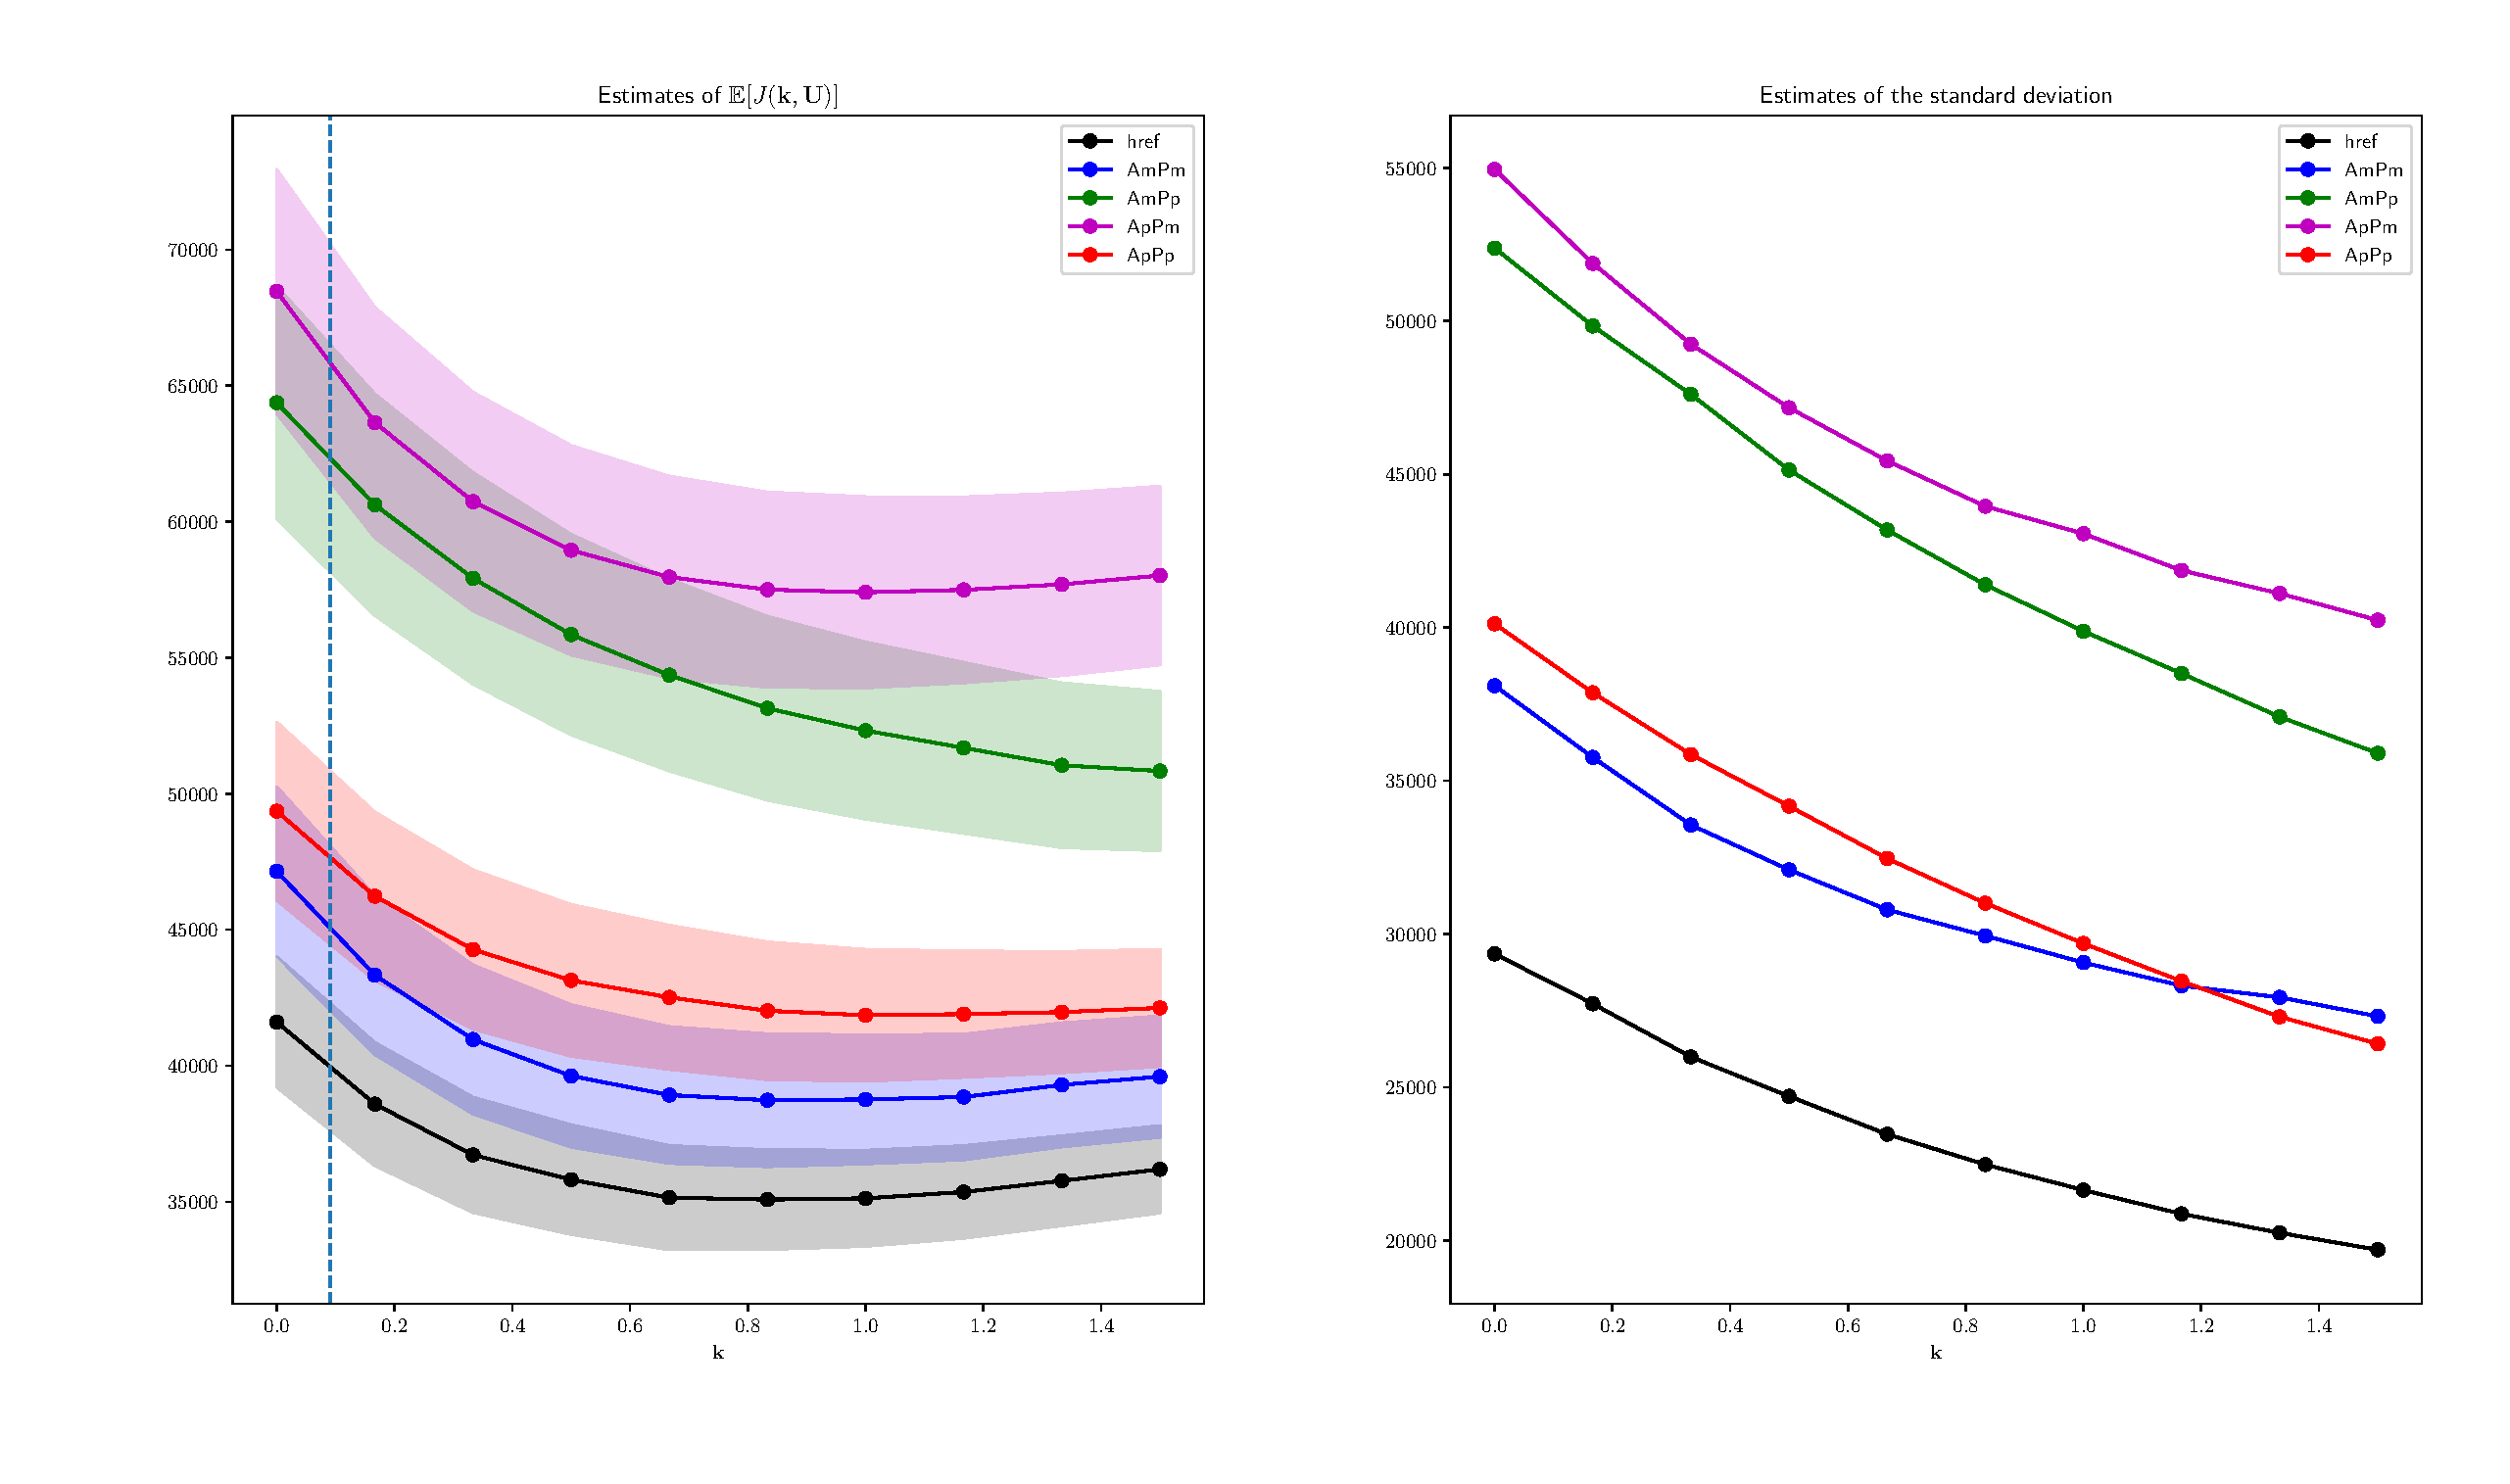
\includegraphics[height = .8\textheight, width = \linewidth]{mean_minimization_illustration}}
%   \end{center}
%   \vspace{-3ex}
%    $\longrightarrow$ Quite different from the value $\kk \approx 0.1$ obtained by optimization knowing the true value of $\uu_{\mathrm{ref}}$ 
% }

\frame{
  \frametitle{``Most Probable Estimate'', and relaxation}%

  \pnote{
    The main idea is that we want to consider individually all situations induced by the value of the environmental variable.
    Basically, once a value u is sampled, the problem is deterministic, so under some assumption, we have a minimiser theta star that is a function of u


    Keeping in mind the random nature of U, we can define the random variable thetastar, and its density (if it is defined), can be seen as the frequency of which a value theta is optimal.


    That is an interesting information, but we can have a little more than that. We may want to include theta that yield values of the cost function close to a minimum. To do that, we introduce a relaxation of the equality constraint with alpha, so that for a given u, we consider acceptable the theta that give values of the cost function between Jstar, the optimal value and alpha times Jstar
    So finally, we compute the probability that this given theta is acceptable with respect to the level alpha
    }
  Given $\uu \sim \UU$, the optimal value is $J^*(\uu)$, attained at
  $\kk^*(\uu) = \argmin_{\kk\in\Kspace} J(\kk,\uu)$.
  \pause
    % \begin{columns}
    %   \begin{column}{0.6\textwidth}

  
      The minimizer can be seen as a random variable:
      \begin{equation*}
        \kk^*(\UU) = \argmin_{\kk\in\Kspace} J(\kk,\alert<1>{\UU})
      \end{equation*}
      $\longrightarrow$ estimate its density (how often is the value $\kk$ a minimizer)
      \begin{align*}
        p_{\kk^*}(\kk)%\,\mathrm{d} \kk & = \Prob\left[\kk^* \in \left[\kk,\kk+\mathrm{d}\kk \right]\right] \\
                                        %        & =\Prob\left[\argmin J(\kk, \uu) \in \left[\kk,\kk+\mathrm{d}\kk \right]\right] \\
                                               &= "\Prob_{\UU}\left[J(\kk,\UU)= J^*(\UU) \right]"                                               % & \Prob\left[ J(\uu) \leq J(\kk, \uu) \forall \kk \in \left[\kk,\kk+\mathrm{d}\kk \right]\right]
      \end{align*}
      \pause
      How to take into account values not optimal, but not too far either
      $\longrightarrow$ relaxation of the equality with $\alpha> 1$:
      \begin{equation*}
        \Gamma_{\alpha}(\kk) = \Prob_{\UU}\left[J(\kk,\UU) \leq \alpha J^*(\UU) \right]
      \end{equation*}
      % \begin{align*}
      %   R(\kk) & = \Prob_{\uu}\left[\kk = \argmin_{\tilde{\kk}} J(\tilde{\kk},\uu) \right] \\
      %   \only<1>{\phantom{R_{\alpha}(\kk)} & = \Prob_{\uu}\left[J(\kk,\uu) \leq \phantom{\alpha}\min_{\tilde{\kk}} J(\tilde{\kk},\uu)\right]}
      %                                           \only<2>{R_{\alert{\alpha}}(\kk) & = \Prob_{\uu}\left[J(\kk,\uu) \leq \alert{\alpha}\min_{\tilde{\kk}} J(\tilde{\kk},\uu)\right]}
      %          \end{align*}%
             % \begin{align*}
             %            R(\kk) &=\Prob_{\uu}\left[\kk = \argmin_{\tilde{\kk}} J(\tilde{\kk},\uu) \right] \\
             %            R_{\alpha}(\kk) & = \Prob_{\uu}\left[J(\kk,\uu) \leq \alpha\min_{\tilde{\kk}} J(\tilde{\kk},\uu)\right]
             %          \end{align*}
             %        }
               % \onslide<2>{$\longrightarrow$ Relaxation of the constraint with $\alpha\geq1$}
                  % \end{column}%
                  % \begin{column}{0.5\textwidth}
                  %   \begin{center}
                  %     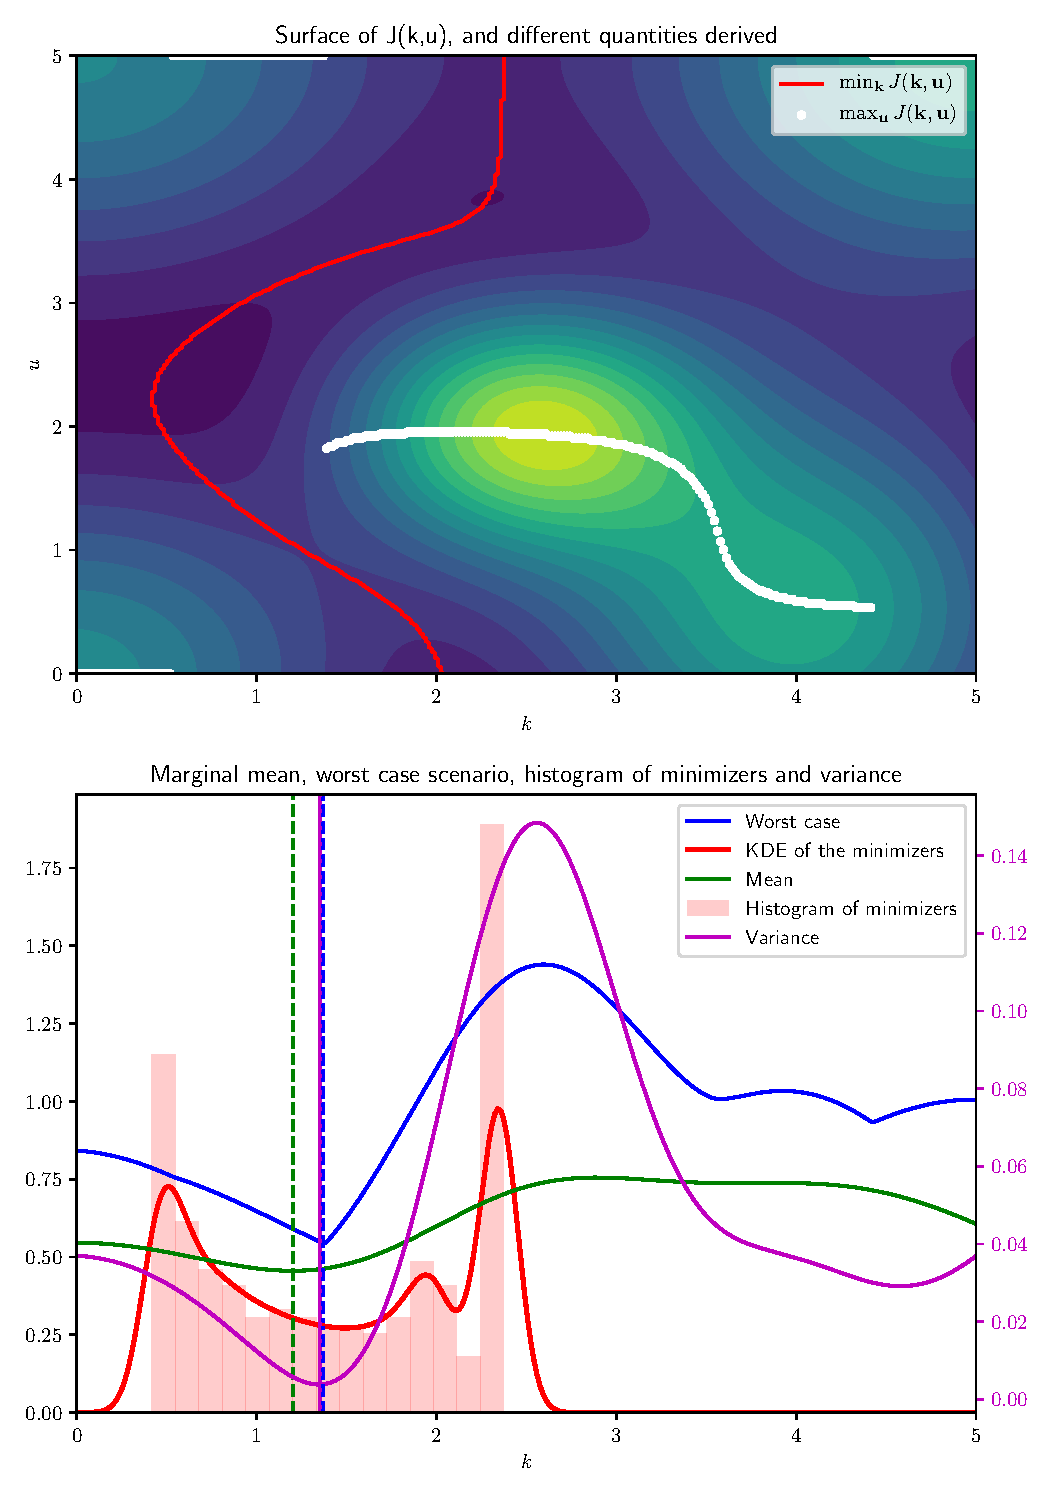
\includegraphics[scale=0.3]{summary_criteria}
                  %   \end{center}
                  %   % \pause
                  %   % Idea: Relaxation of the constraint:
                  %   % \begin{equation*}
                  %   %   R_{\alpha}(\kk) = \Prob\left[J(\kk,\uu) \leq \alpha \min_{\tilde{\kk}} J(\tilde{\kk},\uu)\right],\quad \alpha \geq 1
                  %   % \end{equation*}
                  %   % and increase $\alpha$ until $\max_{\kk} R_{\alpha}(\kk)$ reaches a level of confidence.
                  % \end{column}
                % \end{columns}   %
    }



 
\begin{frame}
  \frametitle{Illustration}
  \pnote{
    What does it look like on a concrete example. We have the plot of a cost function, where theta is the x axis, and u is on the y axis.

    As said earlier, for each horizontal cross section, so for u fixed, we compute the minimiser, theta star of u.

    We can then compute the whole set of the conditional minimisers

    Now, we set alpha: inside the yellow lines, we are between the minimum and alpha times the minimum

    Finally, we construct and measure for each theta the probability to be within this acceptable region.
   Great, now we just have to know how to choose alpha. % Recalling that Gamma here is a probability, we can set levels of interests, such as 1, 0.9 or 0.95 for instance, and take the smallest alpha such that there is a value k where gamma of alpha and k reaches this level, similarly to a quantile.
 }
  \begin{columns}
    \begin{column}{0.45\textwidth}
      \vfill
      \only<1>{\resizebox{\linewidth}{!}{\input{/home/victor/Bureau/tmp/relaxation_tuto_1.pgf}}}%
      \only<2>{\resizebox{\linewidth}{!}{\input{/home/victor/Bureau/tmp/relaxation_tuto_2.pgf}}}%
      \only<3>{\resizebox{\linewidth}{!}{\input{/home/victor/Bureau/tmp/relaxation_tuto_3.pgf}}}
      \only<4>{\resizebox{\linewidth}{!}{\input{/home/victor/Bureau/tmp/relaxation_tuto_4.pgf}}}%
      \vfill
\end{column}
\begin{column}{.6\textwidth}
  \begin{itemize}
  \item<1-> Sample $\uu\sim\UU$, and solve
    $\kk^*(\uu) = \argmin_{\kk\in\Kspace} J(\kk,\uu)$
  \item<2->Set of conditional minimisers: $\{(\kk^*(\uu), \uu) \mid \uu \in \Uspace\}$
  \item<3-> Set $\alpha \geq 1$
  \item<4> $R_{\alpha}(\kk) = \{\uu \mid J(\kk,\uu) \leq \alpha J^*(\uu) \}$
  \item<4> $\Gamma_{\alpha}(\kk) = \Prob_{\UU}\left[\UU\in R_{\alpha}(\kk) \right]$
  % \onslide<5->{\item How to choose $\alpha$? When $\max_{\kk} \Gamma_\alpha(\kk)$ reaches fixed levels}
  \end{itemize}
\end{column}
\end{columns}
\end{frame}

% \frame{
% \frametitle{Illustration of the relaxation}
% \begin{center}
% \scalebox{0.45}{%
% %% Creator: Matplotlib, PGF backend
%%
%% To include the figure in your LaTeX document, write
%%   \input{<filename>.pgf}
%%
%% Make sure the required packages are loaded in your preamble
%%   \usepackage{pgf}
%%
%% Figures using additional raster images can only be included by \input if
%% they are in the same directory as the main LaTeX file. For loading figures
%% from other directories you can use the `import` package
%%   \usepackage{import}
%% and then include the figures with
%%   \import{<path to file>}{<filename>.pgf}
%%
%% Matplotlib used the following preamble
%%   \usepackage{fontspec}
%%   \setmainfont{DejaVu Serif}
%%   \setsansfont{DejaVu Sans}
%%   \setmonofont{DejaVu Sans Mono}
%%
\begingroup%
\makeatletter%
\begin{pgfpicture}%
\pgfpathrectangle{\pgfpointorigin}{\pgfqpoint{9.340000in}{6.020000in}}%
\pgfusepath{use as bounding box, clip}%
\begin{pgfscope}%
\pgfsetbuttcap%
\pgfsetmiterjoin%
\definecolor{currentfill}{rgb}{1.000000,1.000000,1.000000}%
\pgfsetfillcolor{currentfill}%
\pgfsetlinewidth{0.000000pt}%
\definecolor{currentstroke}{rgb}{1.000000,1.000000,1.000000}%
\pgfsetstrokecolor{currentstroke}%
\pgfsetdash{}{0pt}%
\pgfpathmoveto{\pgfqpoint{0.000000in}{0.000000in}}%
\pgfpathlineto{\pgfqpoint{9.340000in}{0.000000in}}%
\pgfpathlineto{\pgfqpoint{9.340000in}{6.020000in}}%
\pgfpathlineto{\pgfqpoint{0.000000in}{6.020000in}}%
\pgfpathclose%
\pgfusepath{fill}%
\end{pgfscope}%
\begin{pgfscope}%
\pgfsetbuttcap%
\pgfsetmiterjoin%
\definecolor{currentfill}{rgb}{1.000000,1.000000,1.000000}%
\pgfsetfillcolor{currentfill}%
\pgfsetlinewidth{0.000000pt}%
\definecolor{currentstroke}{rgb}{0.000000,0.000000,0.000000}%
\pgfsetstrokecolor{currentstroke}%
\pgfsetstrokeopacity{0.000000}%
\pgfsetdash{}{0pt}%
\pgfpathmoveto{\pgfqpoint{0.848113in}{0.730900in}}%
\pgfpathlineto{\pgfqpoint{9.011271in}{0.730900in}}%
\pgfpathlineto{\pgfqpoint{9.011271in}{5.526350in}}%
\pgfpathlineto{\pgfqpoint{0.848113in}{5.526350in}}%
\pgfpathclose%
\pgfusepath{fill}%
\end{pgfscope}%
\begin{pgfscope}%
\pgfpathrectangle{\pgfqpoint{0.848113in}{0.730900in}}{\pgfqpoint{8.163158in}{4.795450in}}%
\pgfusepath{clip}%
\pgfsetbuttcap%
\pgfsetmiterjoin%
\definecolor{currentfill}{rgb}{0.000000,0.000000,1.000000}%
\pgfsetfillcolor{currentfill}%
\pgfsetfillopacity{0.100000}%
\pgfsetlinewidth{1.003750pt}%
\definecolor{currentstroke}{rgb}{0.000000,0.000000,1.000000}%
\pgfsetstrokecolor{currentstroke}%
\pgfsetstrokeopacity{0.100000}%
\pgfsetdash{}{0pt}%
\pgfpathmoveto{\pgfqpoint{1.376659in}{0.730900in}}%
\pgfpathlineto{\pgfqpoint{1.376659in}{5.526350in}}%
\pgfpathlineto{\pgfqpoint{1.704830in}{5.526350in}}%
\pgfpathlineto{\pgfqpoint{1.704830in}{0.730900in}}%
\pgfpathclose%
\pgfusepath{stroke,fill}%
\end{pgfscope}%
\begin{pgfscope}%
\pgfpathrectangle{\pgfqpoint{0.848113in}{0.730900in}}{\pgfqpoint{8.163158in}{4.795450in}}%
\pgfusepath{clip}%
\pgfsetbuttcap%
\pgfsetmiterjoin%
\definecolor{currentfill}{rgb}{0.000000,0.500000,0.000000}%
\pgfsetfillcolor{currentfill}%
\pgfsetfillopacity{0.100000}%
\pgfsetlinewidth{1.003750pt}%
\definecolor{currentstroke}{rgb}{0.000000,0.500000,0.000000}%
\pgfsetstrokecolor{currentstroke}%
\pgfsetstrokeopacity{0.100000}%
\pgfsetdash{}{0pt}%
\pgfpathmoveto{\pgfqpoint{2.024050in}{0.730900in}}%
\pgfpathlineto{\pgfqpoint{2.024050in}{5.526350in}}%
\pgfpathlineto{\pgfqpoint{6.103755in}{5.526350in}}%
\pgfpathlineto{\pgfqpoint{6.103755in}{0.730900in}}%
\pgfpathclose%
\pgfusepath{stroke,fill}%
\end{pgfscope}%
\begin{pgfscope}%
\pgfpathrectangle{\pgfqpoint{0.848113in}{0.730900in}}{\pgfqpoint{8.163158in}{4.795450in}}%
\pgfusepath{clip}%
\pgfsetbuttcap%
\pgfsetmiterjoin%
\definecolor{currentfill}{rgb}{1.000000,0.000000,0.000000}%
\pgfsetfillcolor{currentfill}%
\pgfsetfillopacity{0.100000}%
\pgfsetlinewidth{1.003750pt}%
\definecolor{currentstroke}{rgb}{1.000000,0.000000,0.000000}%
\pgfsetstrokecolor{currentstroke}%
\pgfsetstrokeopacity{0.100000}%
\pgfsetdash{}{0pt}%
\pgfpathmoveto{\pgfqpoint{5.351249in}{0.730900in}}%
\pgfpathlineto{\pgfqpoint{5.351249in}{5.526350in}}%
\pgfpathlineto{\pgfqpoint{7.723924in}{5.526350in}}%
\pgfpathlineto{\pgfqpoint{7.723924in}{0.730900in}}%
\pgfpathclose%
\pgfusepath{stroke,fill}%
\end{pgfscope}%
\begin{pgfscope}%
\pgfsetbuttcap%
\pgfsetroundjoin%
\definecolor{currentfill}{rgb}{0.000000,0.000000,0.000000}%
\pgfsetfillcolor{currentfill}%
\pgfsetlinewidth{0.803000pt}%
\definecolor{currentstroke}{rgb}{0.000000,0.000000,0.000000}%
\pgfsetstrokecolor{currentstroke}%
\pgfsetdash{}{0pt}%
\pgfsys@defobject{currentmarker}{\pgfqpoint{0.000000in}{-0.048611in}}{\pgfqpoint{0.000000in}{0.000000in}}{%
\pgfpathmoveto{\pgfqpoint{0.000000in}{0.000000in}}%
\pgfpathlineto{\pgfqpoint{0.000000in}{-0.048611in}}%
\pgfusepath{stroke,fill}%
}%
\begin{pgfscope}%
\pgfsys@transformshift{1.590218in}{0.730900in}%
\pgfsys@useobject{currentmarker}{}%
\end{pgfscope}%
\end{pgfscope}%
\begin{pgfscope}%
\pgftext[x=1.590218in,y=0.633678in,,top]{\sffamily\fontsize{10.000000}{12.000000}\selectfont \(\displaystyle 0\)}%
\end{pgfscope}%
\begin{pgfscope}%
\pgfsetbuttcap%
\pgfsetroundjoin%
\definecolor{currentfill}{rgb}{0.000000,0.000000,0.000000}%
\pgfsetfillcolor{currentfill}%
\pgfsetlinewidth{0.803000pt}%
\definecolor{currentstroke}{rgb}{0.000000,0.000000,0.000000}%
\pgfsetstrokecolor{currentstroke}%
\pgfsetdash{}{0pt}%
\pgfsys@defobject{currentmarker}{\pgfqpoint{0.000000in}{-0.048611in}}{\pgfqpoint{0.000000in}{0.000000in}}{%
\pgfpathmoveto{\pgfqpoint{0.000000in}{0.000000in}}%
\pgfpathlineto{\pgfqpoint{0.000000in}{-0.048611in}}%
\pgfusepath{stroke,fill}%
}%
\begin{pgfscope}%
\pgfsys@transformshift{3.074429in}{0.730900in}%
\pgfsys@useobject{currentmarker}{}%
\end{pgfscope}%
\end{pgfscope}%
\begin{pgfscope}%
\pgftext[x=3.074429in,y=0.633678in,,top]{\sffamily\fontsize{10.000000}{12.000000}\selectfont \(\displaystyle 1\)}%
\end{pgfscope}%
\begin{pgfscope}%
\pgfsetbuttcap%
\pgfsetroundjoin%
\definecolor{currentfill}{rgb}{0.000000,0.000000,0.000000}%
\pgfsetfillcolor{currentfill}%
\pgfsetlinewidth{0.803000pt}%
\definecolor{currentstroke}{rgb}{0.000000,0.000000,0.000000}%
\pgfsetstrokecolor{currentstroke}%
\pgfsetdash{}{0pt}%
\pgfsys@defobject{currentmarker}{\pgfqpoint{0.000000in}{-0.048611in}}{\pgfqpoint{0.000000in}{0.000000in}}{%
\pgfpathmoveto{\pgfqpoint{0.000000in}{0.000000in}}%
\pgfpathlineto{\pgfqpoint{0.000000in}{-0.048611in}}%
\pgfusepath{stroke,fill}%
}%
\begin{pgfscope}%
\pgfsys@transformshift{4.558639in}{0.730900in}%
\pgfsys@useobject{currentmarker}{}%
\end{pgfscope}%
\end{pgfscope}%
\begin{pgfscope}%
\pgftext[x=4.558639in,y=0.633678in,,top]{\sffamily\fontsize{10.000000}{12.000000}\selectfont \(\displaystyle 2\)}%
\end{pgfscope}%
\begin{pgfscope}%
\pgfsetbuttcap%
\pgfsetroundjoin%
\definecolor{currentfill}{rgb}{0.000000,0.000000,0.000000}%
\pgfsetfillcolor{currentfill}%
\pgfsetlinewidth{0.803000pt}%
\definecolor{currentstroke}{rgb}{0.000000,0.000000,0.000000}%
\pgfsetstrokecolor{currentstroke}%
\pgfsetdash{}{0pt}%
\pgfsys@defobject{currentmarker}{\pgfqpoint{0.000000in}{-0.048611in}}{\pgfqpoint{0.000000in}{0.000000in}}{%
\pgfpathmoveto{\pgfqpoint{0.000000in}{0.000000in}}%
\pgfpathlineto{\pgfqpoint{0.000000in}{-0.048611in}}%
\pgfusepath{stroke,fill}%
}%
\begin{pgfscope}%
\pgfsys@transformshift{6.042850in}{0.730900in}%
\pgfsys@useobject{currentmarker}{}%
\end{pgfscope}%
\end{pgfscope}%
\begin{pgfscope}%
\pgftext[x=6.042850in,y=0.633678in,,top]{\sffamily\fontsize{10.000000}{12.000000}\selectfont \(\displaystyle 3\)}%
\end{pgfscope}%
\begin{pgfscope}%
\pgfsetbuttcap%
\pgfsetroundjoin%
\definecolor{currentfill}{rgb}{0.000000,0.000000,0.000000}%
\pgfsetfillcolor{currentfill}%
\pgfsetlinewidth{0.803000pt}%
\definecolor{currentstroke}{rgb}{0.000000,0.000000,0.000000}%
\pgfsetstrokecolor{currentstroke}%
\pgfsetdash{}{0pt}%
\pgfsys@defobject{currentmarker}{\pgfqpoint{0.000000in}{-0.048611in}}{\pgfqpoint{0.000000in}{0.000000in}}{%
\pgfpathmoveto{\pgfqpoint{0.000000in}{0.000000in}}%
\pgfpathlineto{\pgfqpoint{0.000000in}{-0.048611in}}%
\pgfusepath{stroke,fill}%
}%
\begin{pgfscope}%
\pgfsys@transformshift{7.527060in}{0.730900in}%
\pgfsys@useobject{currentmarker}{}%
\end{pgfscope}%
\end{pgfscope}%
\begin{pgfscope}%
\pgftext[x=7.527060in,y=0.633678in,,top]{\sffamily\fontsize{10.000000}{12.000000}\selectfont \(\displaystyle 4\)}%
\end{pgfscope}%
\begin{pgfscope}%
\pgfsetbuttcap%
\pgfsetroundjoin%
\definecolor{currentfill}{rgb}{0.000000,0.000000,0.000000}%
\pgfsetfillcolor{currentfill}%
\pgfsetlinewidth{0.803000pt}%
\definecolor{currentstroke}{rgb}{0.000000,0.000000,0.000000}%
\pgfsetstrokecolor{currentstroke}%
\pgfsetdash{}{0pt}%
\pgfsys@defobject{currentmarker}{\pgfqpoint{0.000000in}{-0.048611in}}{\pgfqpoint{0.000000in}{0.000000in}}{%
\pgfpathmoveto{\pgfqpoint{0.000000in}{0.000000in}}%
\pgfpathlineto{\pgfqpoint{0.000000in}{-0.048611in}}%
\pgfusepath{stroke,fill}%
}%
\begin{pgfscope}%
\pgfsys@transformshift{9.011271in}{0.730900in}%
\pgfsys@useobject{currentmarker}{}%
\end{pgfscope}%
\end{pgfscope}%
\begin{pgfscope}%
\pgftext[x=9.011271in,y=0.633678in,,top]{\sffamily\fontsize{10.000000}{12.000000}\selectfont \(\displaystyle 5\)}%
\end{pgfscope}%
\begin{pgfscope}%
\pgftext[x=4.929692in,y=0.443710in,,top]{\sffamily\fontsize{10.000000}{12.000000}\selectfont \(\displaystyle {k}\)}%
\end{pgfscope}%
\begin{pgfscope}%
\pgfsetbuttcap%
\pgfsetroundjoin%
\definecolor{currentfill}{rgb}{0.000000,0.000000,0.000000}%
\pgfsetfillcolor{currentfill}%
\pgfsetlinewidth{0.803000pt}%
\definecolor{currentstroke}{rgb}{0.000000,0.000000,0.000000}%
\pgfsetstrokecolor{currentstroke}%
\pgfsetdash{}{0pt}%
\pgfsys@defobject{currentmarker}{\pgfqpoint{-0.048611in}{0.000000in}}{\pgfqpoint{0.000000in}{0.000000in}}{%
\pgfpathmoveto{\pgfqpoint{0.000000in}{0.000000in}}%
\pgfpathlineto{\pgfqpoint{-0.048611in}{0.000000in}}%
\pgfusepath{stroke,fill}%
}%
\begin{pgfscope}%
\pgfsys@transformshift{0.848113in}{0.730900in}%
\pgfsys@useobject{currentmarker}{}%
\end{pgfscope}%
\end{pgfscope}%
\begin{pgfscope}%
\pgftext[x=0.681446in,y=0.678139in,left,base]{\sffamily\fontsize{10.000000}{12.000000}\selectfont \(\displaystyle 0\)}%
\end{pgfscope}%
\begin{pgfscope}%
\pgfsetbuttcap%
\pgfsetroundjoin%
\definecolor{currentfill}{rgb}{0.000000,0.000000,0.000000}%
\pgfsetfillcolor{currentfill}%
\pgfsetlinewidth{0.803000pt}%
\definecolor{currentstroke}{rgb}{0.000000,0.000000,0.000000}%
\pgfsetstrokecolor{currentstroke}%
\pgfsetdash{}{0pt}%
\pgfsys@defobject{currentmarker}{\pgfqpoint{-0.048611in}{0.000000in}}{\pgfqpoint{0.000000in}{0.000000in}}{%
\pgfpathmoveto{\pgfqpoint{0.000000in}{0.000000in}}%
\pgfpathlineto{\pgfqpoint{-0.048611in}{0.000000in}}%
\pgfusepath{stroke,fill}%
}%
\begin{pgfscope}%
\pgfsys@transformshift{0.848113in}{1.689990in}%
\pgfsys@useobject{currentmarker}{}%
\end{pgfscope}%
\end{pgfscope}%
\begin{pgfscope}%
\pgftext[x=0.681446in,y=1.637229in,left,base]{\sffamily\fontsize{10.000000}{12.000000}\selectfont \(\displaystyle 2\)}%
\end{pgfscope}%
\begin{pgfscope}%
\pgfsetbuttcap%
\pgfsetroundjoin%
\definecolor{currentfill}{rgb}{0.000000,0.000000,0.000000}%
\pgfsetfillcolor{currentfill}%
\pgfsetlinewidth{0.803000pt}%
\definecolor{currentstroke}{rgb}{0.000000,0.000000,0.000000}%
\pgfsetstrokecolor{currentstroke}%
\pgfsetdash{}{0pt}%
\pgfsys@defobject{currentmarker}{\pgfqpoint{-0.048611in}{0.000000in}}{\pgfqpoint{0.000000in}{0.000000in}}{%
\pgfpathmoveto{\pgfqpoint{0.000000in}{0.000000in}}%
\pgfpathlineto{\pgfqpoint{-0.048611in}{0.000000in}}%
\pgfusepath{stroke,fill}%
}%
\begin{pgfscope}%
\pgfsys@transformshift{0.848113in}{2.649080in}%
\pgfsys@useobject{currentmarker}{}%
\end{pgfscope}%
\end{pgfscope}%
\begin{pgfscope}%
\pgftext[x=0.681446in,y=2.596319in,left,base]{\sffamily\fontsize{10.000000}{12.000000}\selectfont \(\displaystyle 4\)}%
\end{pgfscope}%
\begin{pgfscope}%
\pgfsetbuttcap%
\pgfsetroundjoin%
\definecolor{currentfill}{rgb}{0.000000,0.000000,0.000000}%
\pgfsetfillcolor{currentfill}%
\pgfsetlinewidth{0.803000pt}%
\definecolor{currentstroke}{rgb}{0.000000,0.000000,0.000000}%
\pgfsetstrokecolor{currentstroke}%
\pgfsetdash{}{0pt}%
\pgfsys@defobject{currentmarker}{\pgfqpoint{-0.048611in}{0.000000in}}{\pgfqpoint{0.000000in}{0.000000in}}{%
\pgfpathmoveto{\pgfqpoint{0.000000in}{0.000000in}}%
\pgfpathlineto{\pgfqpoint{-0.048611in}{0.000000in}}%
\pgfusepath{stroke,fill}%
}%
\begin{pgfscope}%
\pgfsys@transformshift{0.848113in}{3.608170in}%
\pgfsys@useobject{currentmarker}{}%
\end{pgfscope}%
\end{pgfscope}%
\begin{pgfscope}%
\pgftext[x=0.681446in,y=3.555409in,left,base]{\sffamily\fontsize{10.000000}{12.000000}\selectfont \(\displaystyle 6\)}%
\end{pgfscope}%
\begin{pgfscope}%
\pgfsetbuttcap%
\pgfsetroundjoin%
\definecolor{currentfill}{rgb}{0.000000,0.000000,0.000000}%
\pgfsetfillcolor{currentfill}%
\pgfsetlinewidth{0.803000pt}%
\definecolor{currentstroke}{rgb}{0.000000,0.000000,0.000000}%
\pgfsetstrokecolor{currentstroke}%
\pgfsetdash{}{0pt}%
\pgfsys@defobject{currentmarker}{\pgfqpoint{-0.048611in}{0.000000in}}{\pgfqpoint{0.000000in}{0.000000in}}{%
\pgfpathmoveto{\pgfqpoint{0.000000in}{0.000000in}}%
\pgfpathlineto{\pgfqpoint{-0.048611in}{0.000000in}}%
\pgfusepath{stroke,fill}%
}%
\begin{pgfscope}%
\pgfsys@transformshift{0.848113in}{4.567260in}%
\pgfsys@useobject{currentmarker}{}%
\end{pgfscope}%
\end{pgfscope}%
\begin{pgfscope}%
\pgftext[x=0.681446in,y=4.514499in,left,base]{\sffamily\fontsize{10.000000}{12.000000}\selectfont \(\displaystyle 8\)}%
\end{pgfscope}%
\begin{pgfscope}%
\pgfsetbuttcap%
\pgfsetroundjoin%
\definecolor{currentfill}{rgb}{0.000000,0.000000,0.000000}%
\pgfsetfillcolor{currentfill}%
\pgfsetlinewidth{0.803000pt}%
\definecolor{currentstroke}{rgb}{0.000000,0.000000,0.000000}%
\pgfsetstrokecolor{currentstroke}%
\pgfsetdash{}{0pt}%
\pgfsys@defobject{currentmarker}{\pgfqpoint{-0.048611in}{0.000000in}}{\pgfqpoint{0.000000in}{0.000000in}}{%
\pgfpathmoveto{\pgfqpoint{0.000000in}{0.000000in}}%
\pgfpathlineto{\pgfqpoint{-0.048611in}{0.000000in}}%
\pgfusepath{stroke,fill}%
}%
\begin{pgfscope}%
\pgfsys@transformshift{0.848113in}{5.526350in}%
\pgfsys@useobject{currentmarker}{}%
\end{pgfscope}%
\end{pgfscope}%
\begin{pgfscope}%
\pgftext[x=0.612002in,y=5.473589in,left,base]{\sffamily\fontsize{10.000000}{12.000000}\selectfont \(\displaystyle 10\)}%
\end{pgfscope}%
\begin{pgfscope}%
\pgftext[x=0.556446in,y=3.128625in,,bottom,rotate=90.000000]{\sffamily\fontsize{10.000000}{12.000000}\selectfont \(\displaystyle J({k},{u}_i)\)}%
\end{pgfscope}%
\begin{pgfscope}%
\pgfpathrectangle{\pgfqpoint{0.848113in}{0.730900in}}{\pgfqpoint{8.163158in}{4.795450in}}%
\pgfusepath{clip}%
\pgfsetrectcap%
\pgfsetroundjoin%
\pgfsetlinewidth{1.505625pt}%
\definecolor{currentstroke}{rgb}{0.000000,0.000000,1.000000}%
\pgfsetstrokecolor{currentstroke}%
\pgfsetdash{}{0pt}%
\pgfpathmoveto{\pgfqpoint{1.023844in}{5.536350in}}%
\pgfpathlineto{\pgfqpoint{1.039960in}{5.264992in}}%
\pgfpathlineto{\pgfqpoint{1.069704in}{4.793056in}}%
\pgfpathlineto{\pgfqpoint{1.099447in}{4.350008in}}%
\pgfpathlineto{\pgfqpoint{1.129191in}{3.935848in}}%
\pgfpathlineto{\pgfqpoint{1.158935in}{3.550577in}}%
\pgfpathlineto{\pgfqpoint{1.188678in}{3.194194in}}%
\pgfpathlineto{\pgfqpoint{1.218422in}{2.866699in}}%
\pgfpathlineto{\pgfqpoint{1.248166in}{2.568092in}}%
\pgfpathlineto{\pgfqpoint{1.277910in}{2.298373in}}%
\pgfpathlineto{\pgfqpoint{1.307653in}{2.057542in}}%
\pgfpathlineto{\pgfqpoint{1.337397in}{1.845599in}}%
\pgfpathlineto{\pgfqpoint{1.367141in}{1.662545in}}%
\pgfpathlineto{\pgfqpoint{1.396884in}{1.508378in}}%
\pgfpathlineto{\pgfqpoint{1.426628in}{1.383100in}}%
\pgfpathlineto{\pgfqpoint{1.456372in}{1.286710in}}%
\pgfpathlineto{\pgfqpoint{1.486115in}{1.219208in}}%
\pgfpathlineto{\pgfqpoint{1.515859in}{1.180594in}}%
\pgfpathlineto{\pgfqpoint{1.545603in}{1.170869in}}%
\pgfpathlineto{\pgfqpoint{1.575347in}{1.190031in}}%
\pgfpathlineto{\pgfqpoint{1.605090in}{1.238082in}}%
\pgfpathlineto{\pgfqpoint{1.634834in}{1.315020in}}%
\pgfpathlineto{\pgfqpoint{1.664578in}{1.420847in}}%
\pgfpathlineto{\pgfqpoint{1.694321in}{1.555562in}}%
\pgfpathlineto{\pgfqpoint{1.724065in}{1.719166in}}%
\pgfpathlineto{\pgfqpoint{1.753809in}{1.911657in}}%
\pgfpathlineto{\pgfqpoint{1.783552in}{2.133036in}}%
\pgfpathlineto{\pgfqpoint{1.813296in}{2.383304in}}%
\pgfpathlineto{\pgfqpoint{1.843040in}{2.662459in}}%
\pgfpathlineto{\pgfqpoint{1.872784in}{2.970503in}}%
\pgfpathlineto{\pgfqpoint{1.902527in}{3.307435in}}%
\pgfpathlineto{\pgfqpoint{1.932271in}{3.673255in}}%
\pgfpathlineto{\pgfqpoint{1.962015in}{4.067964in}}%
\pgfpathlineto{\pgfqpoint{1.991758in}{4.491560in}}%
\pgfpathlineto{\pgfqpoint{2.021502in}{4.944044in}}%
\pgfpathlineto{\pgfqpoint{2.057712in}{5.536350in}}%
\pgfpathlineto{\pgfqpoint{2.057712in}{5.536350in}}%
\pgfusepath{stroke}%
\end{pgfscope}%
\begin{pgfscope}%
\pgfpathrectangle{\pgfqpoint{0.848113in}{0.730900in}}{\pgfqpoint{8.163158in}{4.795450in}}%
\pgfusepath{clip}%
\pgfsetrectcap%
\pgfsetroundjoin%
\pgfsetlinewidth{1.505625pt}%
\definecolor{currentstroke}{rgb}{1.000000,0.000000,0.000000}%
\pgfsetstrokecolor{currentstroke}%
\pgfsetdash{}{0pt}%
\pgfpathmoveto{\pgfqpoint{4.098177in}{5.536350in}}%
\pgfpathlineto{\pgfqpoint{4.163048in}{5.332319in}}%
\pgfpathlineto{\pgfqpoint{4.252279in}{5.060770in}}%
\pgfpathlineto{\pgfqpoint{4.341510in}{4.799622in}}%
\pgfpathlineto{\pgfqpoint{4.400998in}{4.631300in}}%
\pgfpathlineto{\pgfqpoint{4.460485in}{4.467601in}}%
\pgfpathlineto{\pgfqpoint{4.519973in}{4.308523in}}%
\pgfpathlineto{\pgfqpoint{4.579460in}{4.154068in}}%
\pgfpathlineto{\pgfqpoint{4.638947in}{4.004235in}}%
\pgfpathlineto{\pgfqpoint{4.698435in}{3.859024in}}%
\pgfpathlineto{\pgfqpoint{4.757922in}{3.718435in}}%
\pgfpathlineto{\pgfqpoint{4.817410in}{3.582468in}}%
\pgfpathlineto{\pgfqpoint{4.876897in}{3.451123in}}%
\pgfpathlineto{\pgfqpoint{4.936384in}{3.324401in}}%
\pgfpathlineto{\pgfqpoint{4.995872in}{3.202300in}}%
\pgfpathlineto{\pgfqpoint{5.055359in}{3.084822in}}%
\pgfpathlineto{\pgfqpoint{5.114847in}{2.971965in}}%
\pgfpathlineto{\pgfqpoint{5.174334in}{2.863731in}}%
\pgfpathlineto{\pgfqpoint{5.233821in}{2.760119in}}%
\pgfpathlineto{\pgfqpoint{5.293309in}{2.661129in}}%
\pgfpathlineto{\pgfqpoint{5.352796in}{2.566761in}}%
\pgfpathlineto{\pgfqpoint{5.412284in}{2.477015in}}%
\pgfpathlineto{\pgfqpoint{5.471771in}{2.391892in}}%
\pgfpathlineto{\pgfqpoint{5.531258in}{2.311390in}}%
\pgfpathlineto{\pgfqpoint{5.590746in}{2.235511in}}%
\pgfpathlineto{\pgfqpoint{5.650233in}{2.164253in}}%
\pgfpathlineto{\pgfqpoint{5.709720in}{2.097618in}}%
\pgfpathlineto{\pgfqpoint{5.769208in}{2.035605in}}%
\pgfpathlineto{\pgfqpoint{5.828695in}{1.978214in}}%
\pgfpathlineto{\pgfqpoint{5.888183in}{1.925445in}}%
\pgfpathlineto{\pgfqpoint{5.947670in}{1.877298in}}%
\pgfpathlineto{\pgfqpoint{6.007157in}{1.833773in}}%
\pgfpathlineto{\pgfqpoint{6.066645in}{1.794870in}}%
\pgfpathlineto{\pgfqpoint{6.126132in}{1.760590in}}%
\pgfpathlineto{\pgfqpoint{6.185620in}{1.730931in}}%
\pgfpathlineto{\pgfqpoint{6.245107in}{1.705895in}}%
\pgfpathlineto{\pgfqpoint{6.304594in}{1.685481in}}%
\pgfpathlineto{\pgfqpoint{6.334338in}{1.677007in}}%
\pgfpathlineto{\pgfqpoint{6.364082in}{1.669688in}}%
\pgfpathlineto{\pgfqpoint{6.393826in}{1.663526in}}%
\pgfpathlineto{\pgfqpoint{6.423569in}{1.658518in}}%
\pgfpathlineto{\pgfqpoint{6.453313in}{1.654666in}}%
\pgfpathlineto{\pgfqpoint{6.483057in}{1.651970in}}%
\pgfpathlineto{\pgfqpoint{6.512800in}{1.650430in}}%
\pgfpathlineto{\pgfqpoint{6.542544in}{1.650044in}}%
\pgfpathlineto{\pgfqpoint{6.572288in}{1.650815in}}%
\pgfpathlineto{\pgfqpoint{6.602031in}{1.652741in}}%
\pgfpathlineto{\pgfqpoint{6.631775in}{1.655822in}}%
\pgfpathlineto{\pgfqpoint{6.661519in}{1.660059in}}%
\pgfpathlineto{\pgfqpoint{6.691263in}{1.665451in}}%
\pgfpathlineto{\pgfqpoint{6.721006in}{1.671999in}}%
\pgfpathlineto{\pgfqpoint{6.750750in}{1.679703in}}%
\pgfpathlineto{\pgfqpoint{6.810237in}{1.698576in}}%
\pgfpathlineto{\pgfqpoint{6.869725in}{1.722072in}}%
\pgfpathlineto{\pgfqpoint{6.929212in}{1.750190in}}%
\pgfpathlineto{\pgfqpoint{6.988699in}{1.782930in}}%
\pgfpathlineto{\pgfqpoint{7.048187in}{1.820292in}}%
\pgfpathlineto{\pgfqpoint{7.107674in}{1.862276in}}%
\pgfpathlineto{\pgfqpoint{7.167162in}{1.908882in}}%
\pgfpathlineto{\pgfqpoint{7.226649in}{1.960110in}}%
\pgfpathlineto{\pgfqpoint{7.286136in}{2.015961in}}%
\pgfpathlineto{\pgfqpoint{7.345624in}{2.076433in}}%
\pgfpathlineto{\pgfqpoint{7.405111in}{2.141528in}}%
\pgfpathlineto{\pgfqpoint{7.464599in}{2.211245in}}%
\pgfpathlineto{\pgfqpoint{7.524086in}{2.285583in}}%
\pgfpathlineto{\pgfqpoint{7.583573in}{2.364544in}}%
\pgfpathlineto{\pgfqpoint{7.643061in}{2.448127in}}%
\pgfpathlineto{\pgfqpoint{7.702548in}{2.536332in}}%
\pgfpathlineto{\pgfqpoint{7.762036in}{2.629160in}}%
\pgfpathlineto{\pgfqpoint{7.821523in}{2.726609in}}%
\pgfpathlineto{\pgfqpoint{7.881010in}{2.828680in}}%
\pgfpathlineto{\pgfqpoint{7.940498in}{2.935374in}}%
\pgfpathlineto{\pgfqpoint{7.999985in}{3.046689in}}%
\pgfpathlineto{\pgfqpoint{8.059473in}{3.162627in}}%
\pgfpathlineto{\pgfqpoint{8.118960in}{3.283187in}}%
\pgfpathlineto{\pgfqpoint{8.178447in}{3.408369in}}%
\pgfpathlineto{\pgfqpoint{8.237935in}{3.538173in}}%
\pgfpathlineto{\pgfqpoint{8.297422in}{3.672599in}}%
\pgfpathlineto{\pgfqpoint{8.356910in}{3.811647in}}%
\pgfpathlineto{\pgfqpoint{8.416397in}{3.955318in}}%
\pgfpathlineto{\pgfqpoint{8.475884in}{4.103610in}}%
\pgfpathlineto{\pgfqpoint{8.535372in}{4.256525in}}%
\pgfpathlineto{\pgfqpoint{8.594859in}{4.414061in}}%
\pgfpathlineto{\pgfqpoint{8.654347in}{4.576220in}}%
\pgfpathlineto{\pgfqpoint{8.713834in}{4.743001in}}%
\pgfpathlineto{\pgfqpoint{8.773321in}{4.914404in}}%
\pgfpathlineto{\pgfqpoint{8.832809in}{5.090429in}}%
\pgfpathlineto{\pgfqpoint{8.922040in}{5.363133in}}%
\pgfpathlineto{\pgfqpoint{8.977000in}{5.536350in}}%
\pgfpathlineto{\pgfqpoint{8.977000in}{5.536350in}}%
\pgfusepath{stroke}%
\end{pgfscope}%
\begin{pgfscope}%
\pgfpathrectangle{\pgfqpoint{0.848113in}{0.730900in}}{\pgfqpoint{8.163158in}{4.795450in}}%
\pgfusepath{clip}%
\pgfsetrectcap%
\pgfsetroundjoin%
\pgfsetlinewidth{1.505625pt}%
\definecolor{currentstroke}{rgb}{0.000000,0.500000,0.000000}%
\pgfsetstrokecolor{currentstroke}%
\pgfsetdash{}{0pt}%
\pgfpathmoveto{\pgfqpoint{0.838113in}{3.109195in}}%
\pgfpathlineto{\pgfqpoint{0.920985in}{3.023000in}}%
\pgfpathlineto{\pgfqpoint{1.010216in}{2.932725in}}%
\pgfpathlineto{\pgfqpoint{1.099447in}{2.845049in}}%
\pgfpathlineto{\pgfqpoint{1.188678in}{2.759974in}}%
\pgfpathlineto{\pgfqpoint{1.277910in}{2.677498in}}%
\pgfpathlineto{\pgfqpoint{1.367141in}{2.597622in}}%
\pgfpathlineto{\pgfqpoint{1.456372in}{2.520347in}}%
\pgfpathlineto{\pgfqpoint{1.545603in}{2.445671in}}%
\pgfpathlineto{\pgfqpoint{1.634834in}{2.373595in}}%
\pgfpathlineto{\pgfqpoint{1.724065in}{2.304119in}}%
\pgfpathlineto{\pgfqpoint{1.813296in}{2.237243in}}%
\pgfpathlineto{\pgfqpoint{1.902527in}{2.172967in}}%
\pgfpathlineto{\pgfqpoint{1.991758in}{2.111291in}}%
\pgfpathlineto{\pgfqpoint{2.080989in}{2.052214in}}%
\pgfpathlineto{\pgfqpoint{2.170221in}{1.995738in}}%
\pgfpathlineto{\pgfqpoint{2.259452in}{1.941862in}}%
\pgfpathlineto{\pgfqpoint{2.348683in}{1.890585in}}%
\pgfpathlineto{\pgfqpoint{2.437914in}{1.841909in}}%
\pgfpathlineto{\pgfqpoint{2.527145in}{1.795832in}}%
\pgfpathlineto{\pgfqpoint{2.616376in}{1.752356in}}%
\pgfpathlineto{\pgfqpoint{2.705607in}{1.711479in}}%
\pgfpathlineto{\pgfqpoint{2.794838in}{1.673202in}}%
\pgfpathlineto{\pgfqpoint{2.884069in}{1.637525in}}%
\pgfpathlineto{\pgfqpoint{2.973300in}{1.604448in}}%
\pgfpathlineto{\pgfqpoint{3.062531in}{1.573971in}}%
\pgfpathlineto{\pgfqpoint{3.151763in}{1.546094in}}%
\pgfpathlineto{\pgfqpoint{3.240994in}{1.520817in}}%
\pgfpathlineto{\pgfqpoint{3.330225in}{1.498140in}}%
\pgfpathlineto{\pgfqpoint{3.419456in}{1.478063in}}%
\pgfpathlineto{\pgfqpoint{3.508687in}{1.460585in}}%
\pgfpathlineto{\pgfqpoint{3.597918in}{1.445708in}}%
\pgfpathlineto{\pgfqpoint{3.687149in}{1.433431in}}%
\pgfpathlineto{\pgfqpoint{3.776380in}{1.423753in}}%
\pgfpathlineto{\pgfqpoint{3.865611in}{1.416675in}}%
\pgfpathlineto{\pgfqpoint{3.954842in}{1.412198in}}%
\pgfpathlineto{\pgfqpoint{4.044073in}{1.410320in}}%
\pgfpathlineto{\pgfqpoint{4.133305in}{1.411042in}}%
\pgfpathlineto{\pgfqpoint{4.222536in}{1.414364in}}%
\pgfpathlineto{\pgfqpoint{4.311767in}{1.420286in}}%
\pgfpathlineto{\pgfqpoint{4.400998in}{1.428808in}}%
\pgfpathlineto{\pgfqpoint{4.490229in}{1.439930in}}%
\pgfpathlineto{\pgfqpoint{4.579460in}{1.453652in}}%
\pgfpathlineto{\pgfqpoint{4.668691in}{1.469974in}}%
\pgfpathlineto{\pgfqpoint{4.757922in}{1.488896in}}%
\pgfpathlineto{\pgfqpoint{4.847153in}{1.510417in}}%
\pgfpathlineto{\pgfqpoint{4.936384in}{1.534539in}}%
\pgfpathlineto{\pgfqpoint{5.025615in}{1.561261in}}%
\pgfpathlineto{\pgfqpoint{5.114847in}{1.590582in}}%
\pgfpathlineto{\pgfqpoint{5.204078in}{1.622503in}}%
\pgfpathlineto{\pgfqpoint{5.293309in}{1.657025in}}%
\pgfpathlineto{\pgfqpoint{5.382540in}{1.694146in}}%
\pgfpathlineto{\pgfqpoint{5.471771in}{1.733867in}}%
\pgfpathlineto{\pgfqpoint{5.561002in}{1.776188in}}%
\pgfpathlineto{\pgfqpoint{5.650233in}{1.821109in}}%
\pgfpathlineto{\pgfqpoint{5.739464in}{1.868630in}}%
\pgfpathlineto{\pgfqpoint{5.828695in}{1.918751in}}%
\pgfpathlineto{\pgfqpoint{5.917926in}{1.971472in}}%
\pgfpathlineto{\pgfqpoint{6.007157in}{2.026793in}}%
\pgfpathlineto{\pgfqpoint{6.096389in}{2.084714in}}%
\pgfpathlineto{\pgfqpoint{6.185620in}{2.145234in}}%
\pgfpathlineto{\pgfqpoint{6.274851in}{2.208355in}}%
\pgfpathlineto{\pgfqpoint{6.364082in}{2.274075in}}%
\pgfpathlineto{\pgfqpoint{6.453313in}{2.342396in}}%
\pgfpathlineto{\pgfqpoint{6.542544in}{2.413316in}}%
\pgfpathlineto{\pgfqpoint{6.631775in}{2.486836in}}%
\pgfpathlineto{\pgfqpoint{6.721006in}{2.562957in}}%
\pgfpathlineto{\pgfqpoint{6.810237in}{2.641677in}}%
\pgfpathlineto{\pgfqpoint{6.899468in}{2.722997in}}%
\pgfpathlineto{\pgfqpoint{6.988699in}{2.806917in}}%
\pgfpathlineto{\pgfqpoint{7.077931in}{2.893437in}}%
\pgfpathlineto{\pgfqpoint{7.167162in}{2.982557in}}%
\pgfpathlineto{\pgfqpoint{7.256393in}{3.074277in}}%
\pgfpathlineto{\pgfqpoint{7.345624in}{3.168596in}}%
\pgfpathlineto{\pgfqpoint{7.434855in}{3.265516in}}%
\pgfpathlineto{\pgfqpoint{7.524086in}{3.365036in}}%
\pgfpathlineto{\pgfqpoint{7.613317in}{3.467155in}}%
\pgfpathlineto{\pgfqpoint{7.702548in}{3.571875in}}%
\pgfpathlineto{\pgfqpoint{7.791779in}{3.679194in}}%
\pgfpathlineto{\pgfqpoint{7.910754in}{3.826331in}}%
\pgfpathlineto{\pgfqpoint{8.029729in}{3.978090in}}%
\pgfpathlineto{\pgfqpoint{8.148704in}{4.134471in}}%
\pgfpathlineto{\pgfqpoint{8.267678in}{4.295474in}}%
\pgfpathlineto{\pgfqpoint{8.386653in}{4.461100in}}%
\pgfpathlineto{\pgfqpoint{8.505628in}{4.631347in}}%
\pgfpathlineto{\pgfqpoint{8.624603in}{4.806217in}}%
\pgfpathlineto{\pgfqpoint{8.743578in}{4.985708in}}%
\pgfpathlineto{\pgfqpoint{8.862552in}{5.169822in}}%
\pgfpathlineto{\pgfqpoint{8.981527in}{5.358558in}}%
\pgfpathlineto{\pgfqpoint{9.011271in}{5.406464in}}%
\pgfpathlineto{\pgfqpoint{9.011271in}{5.406464in}}%
\pgfusepath{stroke}%
\end{pgfscope}%
\begin{pgfscope}%
\pgfpathrectangle{\pgfqpoint{0.848113in}{0.730900in}}{\pgfqpoint{8.163158in}{4.795450in}}%
\pgfusepath{clip}%
\pgfsetbuttcap%
\pgfsetroundjoin%
\definecolor{currentfill}{rgb}{0.000000,0.000000,1.000000}%
\pgfsetfillcolor{currentfill}%
\pgfsetlinewidth{1.003750pt}%
\definecolor{currentstroke}{rgb}{0.000000,0.000000,1.000000}%
\pgfsetstrokecolor{currentstroke}%
\pgfsetdash{}{0pt}%
\pgfsys@defobject{currentmarker}{\pgfqpoint{-0.041667in}{-0.041667in}}{\pgfqpoint{0.041667in}{0.041667in}}{%
\pgfpathmoveto{\pgfqpoint{0.000000in}{-0.041667in}}%
\pgfpathcurveto{\pgfqpoint{0.011050in}{-0.041667in}}{\pgfqpoint{0.021649in}{-0.037276in}}{\pgfqpoint{0.029463in}{-0.029463in}}%
\pgfpathcurveto{\pgfqpoint{0.037276in}{-0.021649in}}{\pgfqpoint{0.041667in}{-0.011050in}}{\pgfqpoint{0.041667in}{0.000000in}}%
\pgfpathcurveto{\pgfqpoint{0.041667in}{0.011050in}}{\pgfqpoint{0.037276in}{0.021649in}}{\pgfqpoint{0.029463in}{0.029463in}}%
\pgfpathcurveto{\pgfqpoint{0.021649in}{0.037276in}}{\pgfqpoint{0.011050in}{0.041667in}}{\pgfqpoint{0.000000in}{0.041667in}}%
\pgfpathcurveto{\pgfqpoint{-0.011050in}{0.041667in}}{\pgfqpoint{-0.021649in}{0.037276in}}{\pgfqpoint{-0.029463in}{0.029463in}}%
\pgfpathcurveto{\pgfqpoint{-0.037276in}{0.021649in}}{\pgfqpoint{-0.041667in}{0.011050in}}{\pgfqpoint{-0.041667in}{0.000000in}}%
\pgfpathcurveto{\pgfqpoint{-0.041667in}{-0.011050in}}{\pgfqpoint{-0.037276in}{-0.021649in}}{\pgfqpoint{-0.029463in}{-0.029463in}}%
\pgfpathcurveto{\pgfqpoint{-0.021649in}{-0.037276in}}{\pgfqpoint{-0.011050in}{-0.041667in}}{\pgfqpoint{0.000000in}{-0.041667in}}%
\pgfpathclose%
\pgfusepath{stroke,fill}%
}%
\begin{pgfscope}%
\pgfsys@transformshift{1.540745in}{1.170483in}%
\pgfsys@useobject{currentmarker}{}%
\end{pgfscope}%
\end{pgfscope}%
\begin{pgfscope}%
\pgfpathrectangle{\pgfqpoint{0.848113in}{0.730900in}}{\pgfqpoint{8.163158in}{4.795450in}}%
\pgfusepath{clip}%
\pgfsetbuttcap%
\pgfsetroundjoin%
\definecolor{currentfill}{rgb}{1.000000,0.000000,0.000000}%
\pgfsetfillcolor{currentfill}%
\pgfsetlinewidth{1.003750pt}%
\definecolor{currentstroke}{rgb}{1.000000,0.000000,0.000000}%
\pgfsetstrokecolor{currentstroke}%
\pgfsetdash{}{0pt}%
\pgfsys@defobject{currentmarker}{\pgfqpoint{-0.041667in}{-0.041667in}}{\pgfqpoint{0.041667in}{0.041667in}}{%
\pgfpathmoveto{\pgfqpoint{0.000000in}{-0.041667in}}%
\pgfpathcurveto{\pgfqpoint{0.011050in}{-0.041667in}}{\pgfqpoint{0.021649in}{-0.037276in}}{\pgfqpoint{0.029463in}{-0.029463in}}%
\pgfpathcurveto{\pgfqpoint{0.037276in}{-0.021649in}}{\pgfqpoint{0.041667in}{-0.011050in}}{\pgfqpoint{0.041667in}{0.000000in}}%
\pgfpathcurveto{\pgfqpoint{0.041667in}{0.011050in}}{\pgfqpoint{0.037276in}{0.021649in}}{\pgfqpoint{0.029463in}{0.029463in}}%
\pgfpathcurveto{\pgfqpoint{0.021649in}{0.037276in}}{\pgfqpoint{0.011050in}{0.041667in}}{\pgfqpoint{0.000000in}{0.041667in}}%
\pgfpathcurveto{\pgfqpoint{-0.011050in}{0.041667in}}{\pgfqpoint{-0.021649in}{0.037276in}}{\pgfqpoint{-0.029463in}{0.029463in}}%
\pgfpathcurveto{\pgfqpoint{-0.037276in}{0.021649in}}{\pgfqpoint{-0.041667in}{0.011050in}}{\pgfqpoint{-0.041667in}{0.000000in}}%
\pgfpathcurveto{\pgfqpoint{-0.041667in}{-0.011050in}}{\pgfqpoint{-0.037276in}{-0.021649in}}{\pgfqpoint{-0.029463in}{-0.029463in}}%
\pgfpathcurveto{\pgfqpoint{-0.021649in}{-0.037276in}}{\pgfqpoint{-0.011050in}{-0.041667in}}{\pgfqpoint{0.000000in}{-0.041667in}}%
\pgfpathclose%
\pgfusepath{stroke,fill}%
}%
\begin{pgfscope}%
\pgfsys@transformshift{6.537587in}{1.650028in}%
\pgfsys@useobject{currentmarker}{}%
\end{pgfscope}%
\end{pgfscope}%
\begin{pgfscope}%
\pgfpathrectangle{\pgfqpoint{0.848113in}{0.730900in}}{\pgfqpoint{8.163158in}{4.795450in}}%
\pgfusepath{clip}%
\pgfsetbuttcap%
\pgfsetroundjoin%
\definecolor{currentfill}{rgb}{0.000000,0.500000,0.000000}%
\pgfsetfillcolor{currentfill}%
\pgfsetlinewidth{1.003750pt}%
\definecolor{currentstroke}{rgb}{0.000000,0.500000,0.000000}%
\pgfsetstrokecolor{currentstroke}%
\pgfsetdash{}{0pt}%
\pgfsys@defobject{currentmarker}{\pgfqpoint{-0.041667in}{-0.041667in}}{\pgfqpoint{0.041667in}{0.041667in}}{%
\pgfpathmoveto{\pgfqpoint{0.000000in}{-0.041667in}}%
\pgfpathcurveto{\pgfqpoint{0.011050in}{-0.041667in}}{\pgfqpoint{0.021649in}{-0.037276in}}{\pgfqpoint{0.029463in}{-0.029463in}}%
\pgfpathcurveto{\pgfqpoint{0.037276in}{-0.021649in}}{\pgfqpoint{0.041667in}{-0.011050in}}{\pgfqpoint{0.041667in}{0.000000in}}%
\pgfpathcurveto{\pgfqpoint{0.041667in}{0.011050in}}{\pgfqpoint{0.037276in}{0.021649in}}{\pgfqpoint{0.029463in}{0.029463in}}%
\pgfpathcurveto{\pgfqpoint{0.021649in}{0.037276in}}{\pgfqpoint{0.011050in}{0.041667in}}{\pgfqpoint{0.000000in}{0.041667in}}%
\pgfpathcurveto{\pgfqpoint{-0.011050in}{0.041667in}}{\pgfqpoint{-0.021649in}{0.037276in}}{\pgfqpoint{-0.029463in}{0.029463in}}%
\pgfpathcurveto{\pgfqpoint{-0.037276in}{0.021649in}}{\pgfqpoint{-0.041667in}{0.011050in}}{\pgfqpoint{-0.041667in}{0.000000in}}%
\pgfpathcurveto{\pgfqpoint{-0.041667in}{-0.011050in}}{\pgfqpoint{-0.037276in}{-0.021649in}}{\pgfqpoint{-0.029463in}{-0.029463in}}%
\pgfpathcurveto{\pgfqpoint{-0.021649in}{-0.037276in}}{\pgfqpoint{-0.011050in}{-0.041667in}}{\pgfqpoint{0.000000in}{-0.041667in}}%
\pgfpathclose%
\pgfusepath{stroke,fill}%
}%
\begin{pgfscope}%
\pgfsys@transformshift{4.063903in}{1.410256in}%
\pgfsys@useobject{currentmarker}{}%
\end{pgfscope}%
\end{pgfscope}%
\begin{pgfscope}%
\pgfpathrectangle{\pgfqpoint{0.848113in}{0.730900in}}{\pgfqpoint{8.163158in}{4.795450in}}%
\pgfusepath{clip}%
\pgfsetbuttcap%
\pgfsetroundjoin%
\pgfsetlinewidth{1.505625pt}%
\definecolor{currentstroke}{rgb}{0.000000,0.000000,1.000000}%
\pgfsetstrokecolor{currentstroke}%
\pgfsetdash{{5.550000pt}{2.400000pt}}{0.000000pt}%
\pgfpathmoveto{\pgfqpoint{1.376659in}{1.610066in}}%
\pgfpathlineto{\pgfqpoint{1.704830in}{1.610066in}}%
\pgfusepath{stroke}%
\end{pgfscope}%
\begin{pgfscope}%
\pgfpathrectangle{\pgfqpoint{0.848113in}{0.730900in}}{\pgfqpoint{8.163158in}{4.795450in}}%
\pgfusepath{clip}%
\pgfsetbuttcap%
\pgfsetroundjoin%
\pgfsetlinewidth{1.505625pt}%
\definecolor{currentstroke}{rgb}{0.000000,0.500000,0.000000}%
\pgfsetstrokecolor{currentstroke}%
\pgfsetdash{{5.550000pt}{2.400000pt}}{0.000000pt}%
\pgfpathmoveto{\pgfqpoint{2.024050in}{2.089611in}}%
\pgfpathlineto{\pgfqpoint{6.103755in}{2.089611in}}%
\pgfusepath{stroke}%
\end{pgfscope}%
\begin{pgfscope}%
\pgfpathrectangle{\pgfqpoint{0.848113in}{0.730900in}}{\pgfqpoint{8.163158in}{4.795450in}}%
\pgfusepath{clip}%
\pgfsetbuttcap%
\pgfsetroundjoin%
\pgfsetlinewidth{1.505625pt}%
\definecolor{currentstroke}{rgb}{1.000000,0.000000,0.000000}%
\pgfsetstrokecolor{currentstroke}%
\pgfsetdash{{5.550000pt}{2.400000pt}}{0.000000pt}%
\pgfpathmoveto{\pgfqpoint{5.351249in}{2.569156in}}%
\pgfpathlineto{\pgfqpoint{7.723924in}{2.569156in}}%
\pgfusepath{stroke}%
\end{pgfscope}%
\begin{pgfscope}%
\pgfsetrectcap%
\pgfsetmiterjoin%
\pgfsetlinewidth{0.803000pt}%
\definecolor{currentstroke}{rgb}{0.000000,0.000000,0.000000}%
\pgfsetstrokecolor{currentstroke}%
\pgfsetdash{}{0pt}%
\pgfpathmoveto{\pgfqpoint{0.848113in}{0.730900in}}%
\pgfpathlineto{\pgfqpoint{0.848113in}{5.526350in}}%
\pgfusepath{stroke}%
\end{pgfscope}%
\begin{pgfscope}%
\pgfsetrectcap%
\pgfsetmiterjoin%
\pgfsetlinewidth{0.803000pt}%
\definecolor{currentstroke}{rgb}{0.000000,0.000000,0.000000}%
\pgfsetstrokecolor{currentstroke}%
\pgfsetdash{}{0pt}%
\pgfpathmoveto{\pgfqpoint{9.011271in}{0.730900in}}%
\pgfpathlineto{\pgfqpoint{9.011271in}{5.526350in}}%
\pgfusepath{stroke}%
\end{pgfscope}%
\begin{pgfscope}%
\pgfsetrectcap%
\pgfsetmiterjoin%
\pgfsetlinewidth{0.803000pt}%
\definecolor{currentstroke}{rgb}{0.000000,0.000000,0.000000}%
\pgfsetstrokecolor{currentstroke}%
\pgfsetdash{}{0pt}%
\pgfpathmoveto{\pgfqpoint{0.848113in}{0.730900in}}%
\pgfpathlineto{\pgfqpoint{9.011271in}{0.730900in}}%
\pgfusepath{stroke}%
\end{pgfscope}%
\begin{pgfscope}%
\pgfsetrectcap%
\pgfsetmiterjoin%
\pgfsetlinewidth{0.803000pt}%
\definecolor{currentstroke}{rgb}{0.000000,0.000000,0.000000}%
\pgfsetstrokecolor{currentstroke}%
\pgfsetdash{}{0pt}%
\pgfpathmoveto{\pgfqpoint{0.848113in}{5.526350in}}%
\pgfpathlineto{\pgfqpoint{9.011271in}{5.526350in}}%
\pgfusepath{stroke}%
\end{pgfscope}%
\begin{pgfscope}%
\definecolor{textcolor}{rgb}{0.000000,0.000000,1.000000}%
\pgfsetstrokecolor{textcolor}%
\pgfsetfillcolor{textcolor}%
\pgftext[x=1.590218in,y=0.970673in,left,base]{\color{textcolor}\sffamily\fontsize{15.000000}{18.000000}\selectfont \(\displaystyle J(k^*_1,u_1)\)}%
\end{pgfscope}%
\begin{pgfscope}%
\definecolor{textcolor}{rgb}{0.000000,0.500000,0.000000}%
\pgfsetstrokecolor{textcolor}%
\pgfsetfillcolor{textcolor}%
\pgftext[x=4.113376in,y=1.546127in,left,base]{\color{textcolor}\sffamily\fontsize{15.000000}{18.000000}\selectfont \(\displaystyle J(k^*_2,u_2)\)}%
\end{pgfscope}%
\begin{pgfscope}%
\definecolor{textcolor}{rgb}{1.000000,0.000000,0.000000}%
\pgfsetstrokecolor{textcolor}%
\pgfsetfillcolor{textcolor}%
\pgftext[x=6.042850in,y=1.210445in,left,base]{\color{textcolor}\sffamily\fontsize{15.000000}{18.000000}\selectfont \(\displaystyle J(k^*_3,u_3)\)}%
\end{pgfscope}%
\begin{pgfscope}%
\pgftext[x=4.929692in,y=5.609684in,,base]{\sffamily\fontsize{12.000000}{14.400000}\selectfont \(\displaystyle J({k},{u}_i)\) for different \(\displaystyle {u}_i\), and regions of \(\displaystyle \mathcal{K}\) where \(\displaystyle J({k},{u}_i)\leq \alpha \min_{\tilde{k}}J(\tilde{k},{u}_i)\)}%
\end{pgfscope}%
\end{pgfpicture}%
\makeatother%
\endgroup%
}
% \end{center}
% }

\begin{frame}
  \pnote{Great so now we have Gamma(theta) which is the probability that theta gives a cost alpha acceptable
    If we have an idea of a threshold we don't want to exceed, so if alpha is known we can maximize the probability of being alpha acceptable

    Or, on the other hand, as gamma is a probability, we can look for the smallest relaxation, where the probability of acceptability reaches a certain confidence 1-eta.

    We can then define the family of relative-regret estimators, which are the maximizers of such a probability of being alpha acceptable.
    Depending on the approach, we can nudge toward optimal performances with small alpha, or risk adverse preference, by setting a bigger relaxation.
  }
  \frametitle{Getting an estimator}
  $\Gamma_{\alpha}(\kk)$: probability that the cost (thus $\kk$) is $\alpha$-acceptable
  \begin{itemize}
  \item If $\alpha$ known, maximize the probability that $\kk$ gives acceptable values:
    \begin{equation}
      \max_{\kk\in\Kspace} \Gamma_{\alpha}(\kk) = \max_{\kk\in\Kspace}\Prob_{\UU}\left[J(\kk, \UU) \leq \alpha J^*(\UU)\right]
    \end{equation}
  \item Set a target probability $1-\eta$, and find the smallest $\alpha$.
    \begin{equation}
      \inf\{ \alpha \mid \max_{\kk\in\Kspace}\Gamma_{\alpha}(\kk) \geq 1 - \eta \}
    \end{equation}
  \end{itemize}

  \begin{block}{Relative-regret family of estimators}
  \begin{equation}
   \left\{ \hat{\kk} \mid \hat{\kk} = \argmax_{\kk \in \Kspace} \Gamma_{\alpha}(\kk), \alpha>1 \right\}
  \end{equation}
\end{block}

\end{frame}
\begin{frame}
  \frametitle{Interpretation}
If we either set $\alpha$ or $\eta$
  \begin{align}
    \hat{\kk} &= \argmax \Gamma_{\alpha} \\
    \max \Gamma_{\alpha} &= \Gamma_{\alpha}(\hat{\kk}) = 1-\eta
    \end{align}
    The maximal \emph{relative regret} $J / J^*$ of the function will be $\alpha$, except for the $100\eta\%$ least favourable cases.
    \begin{itemize}
    \item $\alpha$ and $\eta$ 
    \end{itemize}
\end{frame}
\begin{frame}
  \frametitle{Why the relative regret ?}
  \pnote{we discussed so far the relative regret, that takes the form of a multiplicative relaxation. Why this over the additive regret ?

    Relative regret takes better into account the magnitude of the cost function, as the region of acceptability grows with alpha AND Jstar. When the situation is already bad, we don't want to put much effort to stay close to the minimum theta star of u. On the other hand, for Jstar close to 0, 
  }

  
  \renewcommand\rmfamily{\sffamily}
  \begin{center}
  \resizebox{.6\textwidth}{!}{%% Creator: Matplotlib, PGF backend
%%
%% To include the figure in your LaTeX document, write
%%   \input{<filename>.pgf}
%%
%% Make sure the required packages are loaded in your preamble
%%   \usepackage{pgf}
%%
%% Figures using additional raster images can only be included by \input if
%% they are in the same directory as the main LaTeX file. For loading figures
%% from other directories you can use the `import` package
%%   \usepackage{import}
%% and then include the figures with
%%   \import{<path to file>}{<filename>.pgf}
%%
%% Matplotlib used the following preamble
%%   \usepackage{fontspec}
%%   \setmainfont{DejaVuSans.ttf}[Path=/home/victor/miniconda3/lib/python3.7/site-packages/matplotlib/mpl-data/fonts/ttf/]
%%   \setsansfont{LiberationSans-Regular.ttf}[Path=/usr/share/fonts/truetype/liberation/]
%%   \setmonofont{DejaVuSansMono.ttf}[Path=/home/victor/miniconda3/lib/python3.7/site-packages/matplotlib/mpl-data/fonts/ttf/]
%%
\begingroup%
\makeatletter%
\begin{pgfpicture}%
\pgfpathrectangle{\pgfpointorigin}{\pgfqpoint{5.748032in}{3.552479in}}%
\pgfusepath{use as bounding box, clip}%
\begin{pgfscope}%
\pgfsetbuttcap%
\pgfsetmiterjoin%
\definecolor{currentfill}{rgb}{1.000000,1.000000,1.000000}%
\pgfsetfillcolor{currentfill}%
\pgfsetlinewidth{0.000000pt}%
\definecolor{currentstroke}{rgb}{1.000000,1.000000,1.000000}%
\pgfsetstrokecolor{currentstroke}%
\pgfsetdash{}{0pt}%
\pgfpathmoveto{\pgfqpoint{0.000000in}{0.000000in}}%
\pgfpathlineto{\pgfqpoint{5.748032in}{0.000000in}}%
\pgfpathlineto{\pgfqpoint{5.748032in}{3.552479in}}%
\pgfpathlineto{\pgfqpoint{0.000000in}{3.552479in}}%
\pgfpathclose%
\pgfusepath{fill}%
\end{pgfscope}%
\begin{pgfscope}%
\pgfsetbuttcap%
\pgfsetmiterjoin%
\definecolor{currentfill}{rgb}{0.917647,0.917647,0.949020}%
\pgfsetfillcolor{currentfill}%
\pgfsetlinewidth{0.000000pt}%
\definecolor{currentstroke}{rgb}{0.000000,0.000000,0.000000}%
\pgfsetstrokecolor{currentstroke}%
\pgfsetstrokeopacity{0.000000}%
\pgfsetdash{}{0pt}%
\pgfpathmoveto{\pgfqpoint{0.602580in}{0.548769in}}%
\pgfpathlineto{\pgfqpoint{2.676020in}{0.548769in}}%
\pgfpathlineto{\pgfqpoint{2.676020in}{3.213446in}}%
\pgfpathlineto{\pgfqpoint{0.602580in}{3.213446in}}%
\pgfpathclose%
\pgfusepath{fill}%
\end{pgfscope}%
\begin{pgfscope}%
\pgfpathrectangle{\pgfqpoint{0.602580in}{0.548769in}}{\pgfqpoint{2.073440in}{2.664678in}}%
\pgfusepath{clip}%
\pgfsetroundcap%
\pgfsetroundjoin%
\pgfsetlinewidth{1.003750pt}%
\definecolor{currentstroke}{rgb}{1.000000,1.000000,1.000000}%
\pgfsetstrokecolor{currentstroke}%
\pgfsetdash{}{0pt}%
\pgfpathmoveto{\pgfqpoint{0.602580in}{0.548769in}}%
\pgfpathlineto{\pgfqpoint{0.602580in}{3.213446in}}%
\pgfusepath{stroke}%
\end{pgfscope}%
\begin{pgfscope}%
\definecolor{textcolor}{rgb}{0.150000,0.150000,0.150000}%
\pgfsetstrokecolor{textcolor}%
\pgfsetfillcolor{textcolor}%
\pgftext[x=0.602580in,y=0.451547in,,top]{\color{textcolor}\rmfamily\fontsize{10.000000}{12.000000}\selectfont \(\displaystyle 0.00\)}%
\end{pgfscope}%
\begin{pgfscope}%
\pgfpathrectangle{\pgfqpoint{0.602580in}{0.548769in}}{\pgfqpoint{2.073440in}{2.664678in}}%
\pgfusepath{clip}%
\pgfsetroundcap%
\pgfsetroundjoin%
\pgfsetlinewidth{1.003750pt}%
\definecolor{currentstroke}{rgb}{1.000000,1.000000,1.000000}%
\pgfsetstrokecolor{currentstroke}%
\pgfsetdash{}{0pt}%
\pgfpathmoveto{\pgfqpoint{1.120940in}{0.548769in}}%
\pgfpathlineto{\pgfqpoint{1.120940in}{3.213446in}}%
\pgfusepath{stroke}%
\end{pgfscope}%
\begin{pgfscope}%
\definecolor{textcolor}{rgb}{0.150000,0.150000,0.150000}%
\pgfsetstrokecolor{textcolor}%
\pgfsetfillcolor{textcolor}%
\pgftext[x=1.120940in,y=0.451547in,,top]{\color{textcolor}\rmfamily\fontsize{10.000000}{12.000000}\selectfont \(\displaystyle 0.25\)}%
\end{pgfscope}%
\begin{pgfscope}%
\pgfpathrectangle{\pgfqpoint{0.602580in}{0.548769in}}{\pgfqpoint{2.073440in}{2.664678in}}%
\pgfusepath{clip}%
\pgfsetroundcap%
\pgfsetroundjoin%
\pgfsetlinewidth{1.003750pt}%
\definecolor{currentstroke}{rgb}{1.000000,1.000000,1.000000}%
\pgfsetstrokecolor{currentstroke}%
\pgfsetdash{}{0pt}%
\pgfpathmoveto{\pgfqpoint{1.639300in}{0.548769in}}%
\pgfpathlineto{\pgfqpoint{1.639300in}{3.213446in}}%
\pgfusepath{stroke}%
\end{pgfscope}%
\begin{pgfscope}%
\definecolor{textcolor}{rgb}{0.150000,0.150000,0.150000}%
\pgfsetstrokecolor{textcolor}%
\pgfsetfillcolor{textcolor}%
\pgftext[x=1.639300in,y=0.451547in,,top]{\color{textcolor}\rmfamily\fontsize{10.000000}{12.000000}\selectfont \(\displaystyle 0.50\)}%
\end{pgfscope}%
\begin{pgfscope}%
\pgfpathrectangle{\pgfqpoint{0.602580in}{0.548769in}}{\pgfqpoint{2.073440in}{2.664678in}}%
\pgfusepath{clip}%
\pgfsetroundcap%
\pgfsetroundjoin%
\pgfsetlinewidth{1.003750pt}%
\definecolor{currentstroke}{rgb}{1.000000,1.000000,1.000000}%
\pgfsetstrokecolor{currentstroke}%
\pgfsetdash{}{0pt}%
\pgfpathmoveto{\pgfqpoint{2.157660in}{0.548769in}}%
\pgfpathlineto{\pgfqpoint{2.157660in}{3.213446in}}%
\pgfusepath{stroke}%
\end{pgfscope}%
\begin{pgfscope}%
\definecolor{textcolor}{rgb}{0.150000,0.150000,0.150000}%
\pgfsetstrokecolor{textcolor}%
\pgfsetfillcolor{textcolor}%
\pgftext[x=2.157660in,y=0.451547in,,top]{\color{textcolor}\rmfamily\fontsize{10.000000}{12.000000}\selectfont \(\displaystyle 0.75\)}%
\end{pgfscope}%
\begin{pgfscope}%
\pgfpathrectangle{\pgfqpoint{0.602580in}{0.548769in}}{\pgfqpoint{2.073440in}{2.664678in}}%
\pgfusepath{clip}%
\pgfsetroundcap%
\pgfsetroundjoin%
\pgfsetlinewidth{1.003750pt}%
\definecolor{currentstroke}{rgb}{1.000000,1.000000,1.000000}%
\pgfsetstrokecolor{currentstroke}%
\pgfsetdash{}{0pt}%
\pgfpathmoveto{\pgfqpoint{2.676020in}{0.548769in}}%
\pgfpathlineto{\pgfqpoint{2.676020in}{3.213446in}}%
\pgfusepath{stroke}%
\end{pgfscope}%
\begin{pgfscope}%
\definecolor{textcolor}{rgb}{0.150000,0.150000,0.150000}%
\pgfsetstrokecolor{textcolor}%
\pgfsetfillcolor{textcolor}%
\pgftext[x=2.676020in,y=0.451547in,,top]{\color{textcolor}\rmfamily\fontsize{10.000000}{12.000000}\selectfont \(\displaystyle 1.00\)}%
\end{pgfscope}%
\begin{pgfscope}%
\definecolor{textcolor}{rgb}{0.150000,0.150000,0.150000}%
\pgfsetstrokecolor{textcolor}%
\pgfsetfillcolor{textcolor}%
\pgftext[x=1.639300in,y=0.261578in,,top]{\color{textcolor}\rmfamily\fontsize{10.000000}{12.000000}\selectfont \(\displaystyle \theta\)}%
\end{pgfscope}%
\begin{pgfscope}%
\pgfpathrectangle{\pgfqpoint{0.602580in}{0.548769in}}{\pgfqpoint{2.073440in}{2.664678in}}%
\pgfusepath{clip}%
\pgfsetroundcap%
\pgfsetroundjoin%
\pgfsetlinewidth{1.003750pt}%
\definecolor{currentstroke}{rgb}{1.000000,1.000000,1.000000}%
\pgfsetstrokecolor{currentstroke}%
\pgfsetdash{}{0pt}%
\pgfpathmoveto{\pgfqpoint{0.602580in}{0.548769in}}%
\pgfpathlineto{\pgfqpoint{2.676020in}{0.548769in}}%
\pgfusepath{stroke}%
\end{pgfscope}%
\begin{pgfscope}%
\definecolor{textcolor}{rgb}{0.150000,0.150000,0.150000}%
\pgfsetstrokecolor{textcolor}%
\pgfsetfillcolor{textcolor}%
\pgftext[x=0.327888in,y=0.496007in,left,base]{\color{textcolor}\rmfamily\fontsize{10.000000}{12.000000}\selectfont \(\displaystyle 0.0\)}%
\end{pgfscope}%
\begin{pgfscope}%
\pgfpathrectangle{\pgfqpoint{0.602580in}{0.548769in}}{\pgfqpoint{2.073440in}{2.664678in}}%
\pgfusepath{clip}%
\pgfsetroundcap%
\pgfsetroundjoin%
\pgfsetlinewidth{1.003750pt}%
\definecolor{currentstroke}{rgb}{1.000000,1.000000,1.000000}%
\pgfsetstrokecolor{currentstroke}%
\pgfsetdash{}{0pt}%
\pgfpathmoveto{\pgfqpoint{0.602580in}{1.081704in}}%
\pgfpathlineto{\pgfqpoint{2.676020in}{1.081704in}}%
\pgfusepath{stroke}%
\end{pgfscope}%
\begin{pgfscope}%
\definecolor{textcolor}{rgb}{0.150000,0.150000,0.150000}%
\pgfsetstrokecolor{textcolor}%
\pgfsetfillcolor{textcolor}%
\pgftext[x=0.327888in,y=1.028943in,left,base]{\color{textcolor}\rmfamily\fontsize{10.000000}{12.000000}\selectfont \(\displaystyle 0.2\)}%
\end{pgfscope}%
\begin{pgfscope}%
\pgfpathrectangle{\pgfqpoint{0.602580in}{0.548769in}}{\pgfqpoint{2.073440in}{2.664678in}}%
\pgfusepath{clip}%
\pgfsetroundcap%
\pgfsetroundjoin%
\pgfsetlinewidth{1.003750pt}%
\definecolor{currentstroke}{rgb}{1.000000,1.000000,1.000000}%
\pgfsetstrokecolor{currentstroke}%
\pgfsetdash{}{0pt}%
\pgfpathmoveto{\pgfqpoint{0.602580in}{1.614640in}}%
\pgfpathlineto{\pgfqpoint{2.676020in}{1.614640in}}%
\pgfusepath{stroke}%
\end{pgfscope}%
\begin{pgfscope}%
\definecolor{textcolor}{rgb}{0.150000,0.150000,0.150000}%
\pgfsetstrokecolor{textcolor}%
\pgfsetfillcolor{textcolor}%
\pgftext[x=0.327888in,y=1.561878in,left,base]{\color{textcolor}\rmfamily\fontsize{10.000000}{12.000000}\selectfont \(\displaystyle 0.4\)}%
\end{pgfscope}%
\begin{pgfscope}%
\pgfpathrectangle{\pgfqpoint{0.602580in}{0.548769in}}{\pgfqpoint{2.073440in}{2.664678in}}%
\pgfusepath{clip}%
\pgfsetroundcap%
\pgfsetroundjoin%
\pgfsetlinewidth{1.003750pt}%
\definecolor{currentstroke}{rgb}{1.000000,1.000000,1.000000}%
\pgfsetstrokecolor{currentstroke}%
\pgfsetdash{}{0pt}%
\pgfpathmoveto{\pgfqpoint{0.602580in}{2.147575in}}%
\pgfpathlineto{\pgfqpoint{2.676020in}{2.147575in}}%
\pgfusepath{stroke}%
\end{pgfscope}%
\begin{pgfscope}%
\definecolor{textcolor}{rgb}{0.150000,0.150000,0.150000}%
\pgfsetstrokecolor{textcolor}%
\pgfsetfillcolor{textcolor}%
\pgftext[x=0.327888in,y=2.094814in,left,base]{\color{textcolor}\rmfamily\fontsize{10.000000}{12.000000}\selectfont \(\displaystyle 0.6\)}%
\end{pgfscope}%
\begin{pgfscope}%
\pgfpathrectangle{\pgfqpoint{0.602580in}{0.548769in}}{\pgfqpoint{2.073440in}{2.664678in}}%
\pgfusepath{clip}%
\pgfsetroundcap%
\pgfsetroundjoin%
\pgfsetlinewidth{1.003750pt}%
\definecolor{currentstroke}{rgb}{1.000000,1.000000,1.000000}%
\pgfsetstrokecolor{currentstroke}%
\pgfsetdash{}{0pt}%
\pgfpathmoveto{\pgfqpoint{0.602580in}{2.680511in}}%
\pgfpathlineto{\pgfqpoint{2.676020in}{2.680511in}}%
\pgfusepath{stroke}%
\end{pgfscope}%
\begin{pgfscope}%
\definecolor{textcolor}{rgb}{0.150000,0.150000,0.150000}%
\pgfsetstrokecolor{textcolor}%
\pgfsetfillcolor{textcolor}%
\pgftext[x=0.327888in,y=2.627749in,left,base]{\color{textcolor}\rmfamily\fontsize{10.000000}{12.000000}\selectfont \(\displaystyle 0.8\)}%
\end{pgfscope}%
\begin{pgfscope}%
\pgfpathrectangle{\pgfqpoint{0.602580in}{0.548769in}}{\pgfqpoint{2.073440in}{2.664678in}}%
\pgfusepath{clip}%
\pgfsetroundcap%
\pgfsetroundjoin%
\pgfsetlinewidth{1.003750pt}%
\definecolor{currentstroke}{rgb}{1.000000,1.000000,1.000000}%
\pgfsetstrokecolor{currentstroke}%
\pgfsetdash{}{0pt}%
\pgfpathmoveto{\pgfqpoint{0.602580in}{3.213446in}}%
\pgfpathlineto{\pgfqpoint{2.676020in}{3.213446in}}%
\pgfusepath{stroke}%
\end{pgfscope}%
\begin{pgfscope}%
\definecolor{textcolor}{rgb}{0.150000,0.150000,0.150000}%
\pgfsetstrokecolor{textcolor}%
\pgfsetfillcolor{textcolor}%
\pgftext[x=0.327888in,y=3.160685in,left,base]{\color{textcolor}\rmfamily\fontsize{10.000000}{12.000000}\selectfont \(\displaystyle 1.0\)}%
\end{pgfscope}%
\begin{pgfscope}%
\definecolor{textcolor}{rgb}{0.150000,0.150000,0.150000}%
\pgfsetstrokecolor{textcolor}%
\pgfsetfillcolor{textcolor}%
\pgftext[x=0.272332in,y=1.881108in,,bottom,rotate=90.000000]{\color{textcolor}\rmfamily\fontsize{10.000000}{12.000000}\selectfont \(\displaystyle u\)}%
\end{pgfscope}%
\begin{pgfscope}%
\pgfpathrectangle{\pgfqpoint{0.602580in}{0.548769in}}{\pgfqpoint{2.073440in}{2.664678in}}%
\pgfusepath{clip}%
\pgfsetbuttcap%
\pgfsetroundjoin%
\definecolor{currentfill}{rgb}{0.282327,0.094955,0.417331}%
\pgfsetfillcolor{currentfill}%
\pgfsetlinewidth{0.000000pt}%
\definecolor{currentstroke}{rgb}{0.000000,0.000000,0.000000}%
\pgfsetstrokecolor{currentstroke}%
\pgfsetdash{}{0pt}%
\pgfpathmoveto{\pgfqpoint{0.605175in}{0.548769in}}%
\pgfpathlineto{\pgfqpoint{0.607770in}{0.548769in}}%
\pgfpathlineto{\pgfqpoint{0.610365in}{0.548769in}}%
\pgfpathlineto{\pgfqpoint{0.612960in}{0.548769in}}%
\pgfpathlineto{\pgfqpoint{0.615555in}{0.548769in}}%
\pgfpathlineto{\pgfqpoint{0.618150in}{0.548769in}}%
\pgfpathlineto{\pgfqpoint{0.620745in}{0.548769in}}%
\pgfpathlineto{\pgfqpoint{0.623340in}{0.548769in}}%
\pgfpathlineto{\pgfqpoint{0.625935in}{0.548769in}}%
\pgfpathlineto{\pgfqpoint{0.628530in}{0.548769in}}%
\pgfpathlineto{\pgfqpoint{0.631125in}{0.548769in}}%
\pgfpathlineto{\pgfqpoint{0.633720in}{0.548769in}}%
\pgfpathlineto{\pgfqpoint{0.636316in}{0.548769in}}%
\pgfpathlineto{\pgfqpoint{0.638911in}{0.548769in}}%
\pgfpathlineto{\pgfqpoint{0.641506in}{0.548769in}}%
\pgfpathlineto{\pgfqpoint{0.644101in}{0.548769in}}%
\pgfpathlineto{\pgfqpoint{0.646696in}{0.548769in}}%
\pgfpathlineto{\pgfqpoint{0.649291in}{0.548769in}}%
\pgfpathlineto{\pgfqpoint{0.651886in}{0.548769in}}%
\pgfpathlineto{\pgfqpoint{0.654481in}{0.548769in}}%
\pgfpathlineto{\pgfqpoint{0.657076in}{0.548769in}}%
\pgfpathlineto{\pgfqpoint{0.659671in}{0.548769in}}%
\pgfpathlineto{\pgfqpoint{0.662266in}{0.548769in}}%
\pgfpathlineto{\pgfqpoint{0.664861in}{0.548769in}}%
\pgfpathlineto{\pgfqpoint{0.667456in}{0.548769in}}%
\pgfpathlineto{\pgfqpoint{0.670051in}{0.548769in}}%
\pgfpathlineto{\pgfqpoint{0.672646in}{0.548769in}}%
\pgfpathlineto{\pgfqpoint{0.675241in}{0.548769in}}%
\pgfpathlineto{\pgfqpoint{0.677836in}{0.548769in}}%
\pgfpathlineto{\pgfqpoint{0.680431in}{0.548769in}}%
\pgfpathlineto{\pgfqpoint{0.683026in}{0.548769in}}%
\pgfpathlineto{\pgfqpoint{0.685621in}{0.548769in}}%
\pgfpathlineto{\pgfqpoint{0.688216in}{0.548769in}}%
\pgfpathlineto{\pgfqpoint{0.690811in}{0.548769in}}%
\pgfpathlineto{\pgfqpoint{0.693406in}{0.548769in}}%
\pgfpathlineto{\pgfqpoint{0.696002in}{0.548769in}}%
\pgfpathlineto{\pgfqpoint{0.698597in}{0.548769in}}%
\pgfpathlineto{\pgfqpoint{0.701192in}{0.548769in}}%
\pgfpathlineto{\pgfqpoint{0.703787in}{0.548769in}}%
\pgfpathlineto{\pgfqpoint{0.706382in}{0.548769in}}%
\pgfpathlineto{\pgfqpoint{0.708977in}{0.548769in}}%
\pgfpathlineto{\pgfqpoint{0.711572in}{0.548769in}}%
\pgfpathlineto{\pgfqpoint{0.714167in}{0.548769in}}%
\pgfpathlineto{\pgfqpoint{0.716762in}{0.548769in}}%
\pgfpathlineto{\pgfqpoint{0.719357in}{0.548769in}}%
\pgfpathlineto{\pgfqpoint{0.721952in}{0.548769in}}%
\pgfpathlineto{\pgfqpoint{0.724547in}{0.548769in}}%
\pgfpathlineto{\pgfqpoint{0.727142in}{0.548769in}}%
\pgfpathlineto{\pgfqpoint{0.729737in}{0.548769in}}%
\pgfpathlineto{\pgfqpoint{0.732332in}{0.548769in}}%
\pgfpathlineto{\pgfqpoint{0.734927in}{0.548769in}}%
\pgfpathlineto{\pgfqpoint{0.737522in}{0.548769in}}%
\pgfpathlineto{\pgfqpoint{0.740117in}{0.548769in}}%
\pgfpathlineto{\pgfqpoint{0.742712in}{0.548769in}}%
\pgfpathlineto{\pgfqpoint{0.745307in}{0.548769in}}%
\pgfpathlineto{\pgfqpoint{0.747902in}{0.548769in}}%
\pgfpathlineto{\pgfqpoint{0.750497in}{0.548769in}}%
\pgfpathlineto{\pgfqpoint{0.753092in}{0.548769in}}%
\pgfpathlineto{\pgfqpoint{0.755688in}{0.548769in}}%
\pgfpathlineto{\pgfqpoint{0.758283in}{0.548769in}}%
\pgfpathlineto{\pgfqpoint{0.760878in}{0.548769in}}%
\pgfpathlineto{\pgfqpoint{0.763473in}{0.548769in}}%
\pgfpathlineto{\pgfqpoint{0.766068in}{0.548769in}}%
\pgfpathlineto{\pgfqpoint{0.768663in}{0.548769in}}%
\pgfpathlineto{\pgfqpoint{0.771258in}{0.548769in}}%
\pgfpathlineto{\pgfqpoint{0.773853in}{0.548769in}}%
\pgfpathlineto{\pgfqpoint{0.776448in}{0.548769in}}%
\pgfpathlineto{\pgfqpoint{0.779043in}{0.548769in}}%
\pgfpathlineto{\pgfqpoint{0.781638in}{0.548769in}}%
\pgfpathlineto{\pgfqpoint{0.784233in}{0.548769in}}%
\pgfpathlineto{\pgfqpoint{0.786828in}{0.548769in}}%
\pgfpathlineto{\pgfqpoint{0.789423in}{0.548769in}}%
\pgfpathlineto{\pgfqpoint{0.792018in}{0.548769in}}%
\pgfpathlineto{\pgfqpoint{0.794613in}{0.548769in}}%
\pgfpathlineto{\pgfqpoint{0.797208in}{0.548769in}}%
\pgfpathlineto{\pgfqpoint{0.799803in}{0.548769in}}%
\pgfpathlineto{\pgfqpoint{0.802398in}{0.548769in}}%
\pgfpathlineto{\pgfqpoint{0.804993in}{0.548769in}}%
\pgfpathlineto{\pgfqpoint{0.807588in}{0.548769in}}%
\pgfpathlineto{\pgfqpoint{0.810183in}{0.548769in}}%
\pgfpathlineto{\pgfqpoint{0.812778in}{0.548769in}}%
\pgfpathlineto{\pgfqpoint{0.815374in}{0.548769in}}%
\pgfpathlineto{\pgfqpoint{0.817969in}{0.548769in}}%
\pgfpathlineto{\pgfqpoint{0.820564in}{0.548769in}}%
\pgfpathlineto{\pgfqpoint{0.823159in}{0.548769in}}%
\pgfpathlineto{\pgfqpoint{0.825754in}{0.548769in}}%
\pgfpathlineto{\pgfqpoint{0.828349in}{0.548769in}}%
\pgfpathlineto{\pgfqpoint{0.830944in}{0.548769in}}%
\pgfpathlineto{\pgfqpoint{0.833539in}{0.548769in}}%
\pgfpathlineto{\pgfqpoint{0.836134in}{0.548769in}}%
\pgfpathlineto{\pgfqpoint{0.838729in}{0.548769in}}%
\pgfpathlineto{\pgfqpoint{0.841324in}{0.548769in}}%
\pgfpathlineto{\pgfqpoint{0.843919in}{0.548769in}}%
\pgfpathlineto{\pgfqpoint{0.846514in}{0.548769in}}%
\pgfpathlineto{\pgfqpoint{0.849109in}{0.548769in}}%
\pgfpathlineto{\pgfqpoint{0.851704in}{0.548769in}}%
\pgfpathlineto{\pgfqpoint{0.854299in}{0.548769in}}%
\pgfpathlineto{\pgfqpoint{0.856894in}{0.548769in}}%
\pgfpathlineto{\pgfqpoint{0.859489in}{0.548769in}}%
\pgfpathlineto{\pgfqpoint{0.862084in}{0.548769in}}%
\pgfpathlineto{\pgfqpoint{0.864679in}{0.548769in}}%
\pgfpathlineto{\pgfqpoint{0.867274in}{0.548769in}}%
\pgfpathlineto{\pgfqpoint{0.869869in}{0.548769in}}%
\pgfpathlineto{\pgfqpoint{0.872464in}{0.548769in}}%
\pgfpathlineto{\pgfqpoint{0.875060in}{0.548769in}}%
\pgfpathlineto{\pgfqpoint{0.877655in}{0.548769in}}%
\pgfpathlineto{\pgfqpoint{0.880250in}{0.548769in}}%
\pgfpathlineto{\pgfqpoint{0.882845in}{0.548769in}}%
\pgfpathlineto{\pgfqpoint{0.885440in}{0.548769in}}%
\pgfpathlineto{\pgfqpoint{0.888035in}{0.548769in}}%
\pgfpathlineto{\pgfqpoint{0.890630in}{0.548769in}}%
\pgfpathlineto{\pgfqpoint{0.893225in}{0.548769in}}%
\pgfpathlineto{\pgfqpoint{0.895820in}{0.548769in}}%
\pgfpathlineto{\pgfqpoint{0.898415in}{0.548769in}}%
\pgfpathlineto{\pgfqpoint{0.901010in}{0.548769in}}%
\pgfpathlineto{\pgfqpoint{0.903605in}{0.548769in}}%
\pgfpathlineto{\pgfqpoint{0.906200in}{0.548769in}}%
\pgfpathlineto{\pgfqpoint{0.908795in}{0.548769in}}%
\pgfpathlineto{\pgfqpoint{0.911390in}{0.548769in}}%
\pgfpathlineto{\pgfqpoint{0.913985in}{0.548769in}}%
\pgfpathlineto{\pgfqpoint{0.916580in}{0.548769in}}%
\pgfpathlineto{\pgfqpoint{0.919175in}{0.548769in}}%
\pgfpathlineto{\pgfqpoint{0.921770in}{0.548769in}}%
\pgfpathlineto{\pgfqpoint{0.924365in}{0.548769in}}%
\pgfpathlineto{\pgfqpoint{0.926960in}{0.548769in}}%
\pgfpathlineto{\pgfqpoint{0.929555in}{0.548769in}}%
\pgfpathlineto{\pgfqpoint{0.932150in}{0.548769in}}%
\pgfpathlineto{\pgfqpoint{0.934746in}{0.548769in}}%
\pgfpathlineto{\pgfqpoint{0.937341in}{0.548769in}}%
\pgfpathlineto{\pgfqpoint{0.939936in}{0.548769in}}%
\pgfpathlineto{\pgfqpoint{0.942531in}{0.548769in}}%
\pgfpathlineto{\pgfqpoint{0.945126in}{0.548769in}}%
\pgfpathlineto{\pgfqpoint{0.947721in}{0.548769in}}%
\pgfpathlineto{\pgfqpoint{0.950316in}{0.548769in}}%
\pgfpathlineto{\pgfqpoint{0.952911in}{0.548769in}}%
\pgfpathlineto{\pgfqpoint{0.955506in}{0.548769in}}%
\pgfpathlineto{\pgfqpoint{0.958101in}{0.548769in}}%
\pgfpathlineto{\pgfqpoint{0.960696in}{0.548769in}}%
\pgfpathlineto{\pgfqpoint{0.963291in}{0.548769in}}%
\pgfpathlineto{\pgfqpoint{0.965886in}{0.548769in}}%
\pgfpathlineto{\pgfqpoint{0.968481in}{0.548769in}}%
\pgfpathlineto{\pgfqpoint{0.971076in}{0.548769in}}%
\pgfpathlineto{\pgfqpoint{0.973671in}{0.548769in}}%
\pgfpathlineto{\pgfqpoint{0.976266in}{0.548769in}}%
\pgfpathlineto{\pgfqpoint{0.978861in}{0.548769in}}%
\pgfpathlineto{\pgfqpoint{0.981456in}{0.548769in}}%
\pgfpathlineto{\pgfqpoint{0.984051in}{0.548769in}}%
\pgfpathlineto{\pgfqpoint{0.986646in}{0.548769in}}%
\pgfpathlineto{\pgfqpoint{0.989241in}{0.548769in}}%
\pgfpathlineto{\pgfqpoint{0.991837in}{0.548769in}}%
\pgfpathlineto{\pgfqpoint{0.994432in}{0.548769in}}%
\pgfpathlineto{\pgfqpoint{0.997027in}{0.548769in}}%
\pgfpathlineto{\pgfqpoint{0.999622in}{0.548769in}}%
\pgfpathlineto{\pgfqpoint{1.002217in}{0.548769in}}%
\pgfpathlineto{\pgfqpoint{1.004812in}{0.548769in}}%
\pgfpathlineto{\pgfqpoint{1.007407in}{0.548769in}}%
\pgfpathlineto{\pgfqpoint{1.010002in}{0.548769in}}%
\pgfpathlineto{\pgfqpoint{1.012597in}{0.548769in}}%
\pgfpathlineto{\pgfqpoint{1.015192in}{0.548769in}}%
\pgfpathlineto{\pgfqpoint{1.017787in}{0.548769in}}%
\pgfpathlineto{\pgfqpoint{1.020382in}{0.548769in}}%
\pgfpathlineto{\pgfqpoint{1.022977in}{0.548769in}}%
\pgfpathlineto{\pgfqpoint{1.025572in}{0.548769in}}%
\pgfpathlineto{\pgfqpoint{1.028167in}{0.548769in}}%
\pgfpathlineto{\pgfqpoint{1.030762in}{0.548769in}}%
\pgfpathlineto{\pgfqpoint{1.033357in}{0.548769in}}%
\pgfpathlineto{\pgfqpoint{1.035952in}{0.548769in}}%
\pgfpathlineto{\pgfqpoint{1.038547in}{0.548769in}}%
\pgfpathlineto{\pgfqpoint{1.041142in}{0.548769in}}%
\pgfpathlineto{\pgfqpoint{1.043737in}{0.548769in}}%
\pgfpathlineto{\pgfqpoint{1.046332in}{0.548769in}}%
\pgfpathlineto{\pgfqpoint{1.048927in}{0.548769in}}%
\pgfpathlineto{\pgfqpoint{1.051523in}{0.548769in}}%
\pgfpathlineto{\pgfqpoint{1.054118in}{0.548769in}}%
\pgfpathlineto{\pgfqpoint{1.056713in}{0.548769in}}%
\pgfpathlineto{\pgfqpoint{1.059308in}{0.548769in}}%
\pgfpathlineto{\pgfqpoint{1.061903in}{0.548769in}}%
\pgfpathlineto{\pgfqpoint{1.064498in}{0.548769in}}%
\pgfpathlineto{\pgfqpoint{1.067093in}{0.548769in}}%
\pgfpathlineto{\pgfqpoint{1.069688in}{0.548769in}}%
\pgfpathlineto{\pgfqpoint{1.072283in}{0.548769in}}%
\pgfpathlineto{\pgfqpoint{1.074878in}{0.548769in}}%
\pgfpathlineto{\pgfqpoint{1.077473in}{0.548769in}}%
\pgfpathlineto{\pgfqpoint{1.080068in}{0.548769in}}%
\pgfpathlineto{\pgfqpoint{1.082663in}{0.548769in}}%
\pgfpathlineto{\pgfqpoint{1.085258in}{0.548769in}}%
\pgfpathlineto{\pgfqpoint{1.087853in}{0.548769in}}%
\pgfpathlineto{\pgfqpoint{1.090448in}{0.548769in}}%
\pgfpathlineto{\pgfqpoint{1.093043in}{0.548769in}}%
\pgfpathlineto{\pgfqpoint{1.095638in}{0.548769in}}%
\pgfpathlineto{\pgfqpoint{1.098233in}{0.548769in}}%
\pgfpathlineto{\pgfqpoint{1.100828in}{0.548769in}}%
\pgfpathlineto{\pgfqpoint{1.103423in}{0.548769in}}%
\pgfpathlineto{\pgfqpoint{1.106018in}{0.548769in}}%
\pgfpathlineto{\pgfqpoint{1.108613in}{0.548769in}}%
\pgfpathlineto{\pgfqpoint{1.111209in}{0.548769in}}%
\pgfpathlineto{\pgfqpoint{1.113804in}{0.548769in}}%
\pgfpathlineto{\pgfqpoint{1.116399in}{0.548769in}}%
\pgfpathlineto{\pgfqpoint{1.118994in}{0.548769in}}%
\pgfpathlineto{\pgfqpoint{1.121589in}{0.548769in}}%
\pgfpathlineto{\pgfqpoint{1.124184in}{0.548769in}}%
\pgfpathlineto{\pgfqpoint{1.126779in}{0.548769in}}%
\pgfpathlineto{\pgfqpoint{1.129374in}{0.548769in}}%
\pgfpathlineto{\pgfqpoint{1.131969in}{0.548769in}}%
\pgfpathlineto{\pgfqpoint{1.134564in}{0.548769in}}%
\pgfpathlineto{\pgfqpoint{1.137159in}{0.548769in}}%
\pgfpathlineto{\pgfqpoint{1.139754in}{0.548769in}}%
\pgfpathlineto{\pgfqpoint{1.142349in}{0.548769in}}%
\pgfpathlineto{\pgfqpoint{1.144944in}{0.548769in}}%
\pgfpathlineto{\pgfqpoint{1.147539in}{0.548769in}}%
\pgfpathlineto{\pgfqpoint{1.150134in}{0.548769in}}%
\pgfpathlineto{\pgfqpoint{1.152729in}{0.548769in}}%
\pgfpathlineto{\pgfqpoint{1.155324in}{0.548769in}}%
\pgfpathlineto{\pgfqpoint{1.157919in}{0.548769in}}%
\pgfpathlineto{\pgfqpoint{1.160514in}{0.548769in}}%
\pgfpathlineto{\pgfqpoint{1.163109in}{0.548769in}}%
\pgfpathlineto{\pgfqpoint{1.165704in}{0.548769in}}%
\pgfpathlineto{\pgfqpoint{1.168299in}{0.548769in}}%
\pgfpathlineto{\pgfqpoint{1.170895in}{0.548769in}}%
\pgfpathlineto{\pgfqpoint{1.173490in}{0.548769in}}%
\pgfpathlineto{\pgfqpoint{1.176085in}{0.548769in}}%
\pgfpathlineto{\pgfqpoint{1.178680in}{0.548769in}}%
\pgfpathlineto{\pgfqpoint{1.181275in}{0.548769in}}%
\pgfpathlineto{\pgfqpoint{1.183870in}{0.548769in}}%
\pgfpathlineto{\pgfqpoint{1.186465in}{0.548769in}}%
\pgfpathlineto{\pgfqpoint{1.189060in}{0.548769in}}%
\pgfpathlineto{\pgfqpoint{1.191655in}{0.548769in}}%
\pgfpathlineto{\pgfqpoint{1.194250in}{0.548769in}}%
\pgfpathlineto{\pgfqpoint{1.196845in}{0.548769in}}%
\pgfpathlineto{\pgfqpoint{1.199440in}{0.548769in}}%
\pgfpathlineto{\pgfqpoint{1.202035in}{0.548769in}}%
\pgfpathlineto{\pgfqpoint{1.204630in}{0.548769in}}%
\pgfpathlineto{\pgfqpoint{1.207225in}{0.548769in}}%
\pgfpathlineto{\pgfqpoint{1.209820in}{0.548769in}}%
\pgfpathlineto{\pgfqpoint{1.212415in}{0.548769in}}%
\pgfpathlineto{\pgfqpoint{1.215010in}{0.548769in}}%
\pgfpathlineto{\pgfqpoint{1.217605in}{0.548769in}}%
\pgfpathlineto{\pgfqpoint{1.220200in}{0.548769in}}%
\pgfpathlineto{\pgfqpoint{1.222795in}{0.548769in}}%
\pgfpathlineto{\pgfqpoint{1.225390in}{0.548769in}}%
\pgfpathlineto{\pgfqpoint{1.227985in}{0.548769in}}%
\pgfpathlineto{\pgfqpoint{1.230581in}{0.548769in}}%
\pgfpathlineto{\pgfqpoint{1.233176in}{0.548769in}}%
\pgfpathlineto{\pgfqpoint{1.235771in}{0.548769in}}%
\pgfpathlineto{\pgfqpoint{1.238366in}{0.548769in}}%
\pgfpathlineto{\pgfqpoint{1.240961in}{0.548769in}}%
\pgfpathlineto{\pgfqpoint{1.243556in}{0.548769in}}%
\pgfpathlineto{\pgfqpoint{1.246151in}{0.548769in}}%
\pgfpathlineto{\pgfqpoint{1.248746in}{0.548769in}}%
\pgfpathlineto{\pgfqpoint{1.251341in}{0.548769in}}%
\pgfpathlineto{\pgfqpoint{1.253936in}{0.548769in}}%
\pgfpathlineto{\pgfqpoint{1.256531in}{0.548769in}}%
\pgfpathlineto{\pgfqpoint{1.259126in}{0.548769in}}%
\pgfpathlineto{\pgfqpoint{1.261721in}{0.548769in}}%
\pgfpathlineto{\pgfqpoint{1.264316in}{0.548769in}}%
\pgfpathlineto{\pgfqpoint{1.266911in}{0.548769in}}%
\pgfpathlineto{\pgfqpoint{1.269506in}{0.548769in}}%
\pgfpathlineto{\pgfqpoint{1.272101in}{0.548769in}}%
\pgfpathlineto{\pgfqpoint{1.274696in}{0.548769in}}%
\pgfpathlineto{\pgfqpoint{1.277291in}{0.548769in}}%
\pgfpathlineto{\pgfqpoint{1.279886in}{0.548769in}}%
\pgfpathlineto{\pgfqpoint{1.282481in}{0.548769in}}%
\pgfpathlineto{\pgfqpoint{1.285076in}{0.548769in}}%
\pgfpathlineto{\pgfqpoint{1.287671in}{0.548769in}}%
\pgfpathlineto{\pgfqpoint{1.290267in}{0.548769in}}%
\pgfpathlineto{\pgfqpoint{1.292862in}{0.548769in}}%
\pgfpathlineto{\pgfqpoint{1.295457in}{0.548769in}}%
\pgfpathlineto{\pgfqpoint{1.298052in}{0.548769in}}%
\pgfpathlineto{\pgfqpoint{1.300647in}{0.548769in}}%
\pgfpathlineto{\pgfqpoint{1.303242in}{0.548769in}}%
\pgfpathlineto{\pgfqpoint{1.305837in}{0.548769in}}%
\pgfpathlineto{\pgfqpoint{1.308432in}{0.548769in}}%
\pgfpathlineto{\pgfqpoint{1.311027in}{0.548769in}}%
\pgfpathlineto{\pgfqpoint{1.313622in}{0.548769in}}%
\pgfpathlineto{\pgfqpoint{1.316217in}{0.548769in}}%
\pgfpathlineto{\pgfqpoint{1.318812in}{0.548769in}}%
\pgfpathlineto{\pgfqpoint{1.321407in}{0.548769in}}%
\pgfpathlineto{\pgfqpoint{1.324002in}{0.548769in}}%
\pgfpathlineto{\pgfqpoint{1.326597in}{0.548769in}}%
\pgfpathlineto{\pgfqpoint{1.329192in}{0.548769in}}%
\pgfpathlineto{\pgfqpoint{1.331787in}{0.548769in}}%
\pgfpathlineto{\pgfqpoint{1.334382in}{0.548769in}}%
\pgfpathlineto{\pgfqpoint{1.336977in}{0.548769in}}%
\pgfpathlineto{\pgfqpoint{1.339572in}{0.548769in}}%
\pgfpathlineto{\pgfqpoint{1.342167in}{0.548769in}}%
\pgfpathlineto{\pgfqpoint{1.344762in}{0.548769in}}%
\pgfpathlineto{\pgfqpoint{1.347358in}{0.548769in}}%
\pgfpathlineto{\pgfqpoint{1.349953in}{0.548769in}}%
\pgfpathlineto{\pgfqpoint{1.352548in}{0.548769in}}%
\pgfpathlineto{\pgfqpoint{1.355143in}{0.548769in}}%
\pgfpathlineto{\pgfqpoint{1.357738in}{0.548769in}}%
\pgfpathlineto{\pgfqpoint{1.360333in}{0.548769in}}%
\pgfpathlineto{\pgfqpoint{1.362928in}{0.548769in}}%
\pgfpathlineto{\pgfqpoint{1.365523in}{0.548769in}}%
\pgfpathlineto{\pgfqpoint{1.368118in}{0.548769in}}%
\pgfpathlineto{\pgfqpoint{1.370713in}{0.548769in}}%
\pgfpathlineto{\pgfqpoint{1.373308in}{0.548769in}}%
\pgfpathlineto{\pgfqpoint{1.375903in}{0.548769in}}%
\pgfpathlineto{\pgfqpoint{1.378498in}{0.548769in}}%
\pgfpathlineto{\pgfqpoint{1.381093in}{0.548769in}}%
\pgfpathlineto{\pgfqpoint{1.383688in}{0.548769in}}%
\pgfpathlineto{\pgfqpoint{1.386283in}{0.548769in}}%
\pgfpathlineto{\pgfqpoint{1.388878in}{0.548769in}}%
\pgfpathlineto{\pgfqpoint{1.391473in}{0.548769in}}%
\pgfpathlineto{\pgfqpoint{1.394068in}{0.548769in}}%
\pgfpathlineto{\pgfqpoint{1.396663in}{0.548769in}}%
\pgfpathlineto{\pgfqpoint{1.399258in}{0.548769in}}%
\pgfpathlineto{\pgfqpoint{1.401853in}{0.548769in}}%
\pgfpathlineto{\pgfqpoint{1.404448in}{0.548769in}}%
\pgfpathlineto{\pgfqpoint{1.407044in}{0.548769in}}%
\pgfpathlineto{\pgfqpoint{1.409639in}{0.548769in}}%
\pgfpathlineto{\pgfqpoint{1.412234in}{0.548769in}}%
\pgfpathlineto{\pgfqpoint{1.414829in}{0.548769in}}%
\pgfpathlineto{\pgfqpoint{1.417424in}{0.548769in}}%
\pgfpathlineto{\pgfqpoint{1.420019in}{0.548769in}}%
\pgfpathlineto{\pgfqpoint{1.422614in}{0.548769in}}%
\pgfpathlineto{\pgfqpoint{1.425209in}{0.548769in}}%
\pgfpathlineto{\pgfqpoint{1.427804in}{0.548769in}}%
\pgfpathlineto{\pgfqpoint{1.430399in}{0.548769in}}%
\pgfpathlineto{\pgfqpoint{1.432994in}{0.548769in}}%
\pgfpathlineto{\pgfqpoint{1.435589in}{0.548769in}}%
\pgfpathlineto{\pgfqpoint{1.438184in}{0.548769in}}%
\pgfpathlineto{\pgfqpoint{1.440779in}{0.548769in}}%
\pgfpathlineto{\pgfqpoint{1.443374in}{0.548769in}}%
\pgfpathlineto{\pgfqpoint{1.445969in}{0.548769in}}%
\pgfpathlineto{\pgfqpoint{1.448564in}{0.548769in}}%
\pgfpathlineto{\pgfqpoint{1.451159in}{0.548769in}}%
\pgfpathlineto{\pgfqpoint{1.453754in}{0.548769in}}%
\pgfpathlineto{\pgfqpoint{1.456349in}{0.548769in}}%
\pgfpathlineto{\pgfqpoint{1.458944in}{0.548769in}}%
\pgfpathlineto{\pgfqpoint{1.461539in}{0.548769in}}%
\pgfpathlineto{\pgfqpoint{1.464134in}{0.548769in}}%
\pgfpathlineto{\pgfqpoint{1.466730in}{0.548769in}}%
\pgfpathlineto{\pgfqpoint{1.469325in}{0.548769in}}%
\pgfpathlineto{\pgfqpoint{1.471920in}{0.548769in}}%
\pgfpathlineto{\pgfqpoint{1.474515in}{0.548769in}}%
\pgfpathlineto{\pgfqpoint{1.477110in}{0.548769in}}%
\pgfpathlineto{\pgfqpoint{1.479705in}{0.548769in}}%
\pgfpathlineto{\pgfqpoint{1.482300in}{0.548769in}}%
\pgfpathlineto{\pgfqpoint{1.484895in}{0.548769in}}%
\pgfpathlineto{\pgfqpoint{1.487490in}{0.548769in}}%
\pgfpathlineto{\pgfqpoint{1.490085in}{0.548769in}}%
\pgfpathlineto{\pgfqpoint{1.492680in}{0.548769in}}%
\pgfpathlineto{\pgfqpoint{1.495275in}{0.548769in}}%
\pgfpathlineto{\pgfqpoint{1.497870in}{0.548769in}}%
\pgfpathlineto{\pgfqpoint{1.500465in}{0.548769in}}%
\pgfpathlineto{\pgfqpoint{1.503060in}{0.548769in}}%
\pgfpathlineto{\pgfqpoint{1.505655in}{0.548769in}}%
\pgfpathlineto{\pgfqpoint{1.508250in}{0.548769in}}%
\pgfpathlineto{\pgfqpoint{1.510845in}{0.548769in}}%
\pgfpathlineto{\pgfqpoint{1.513440in}{0.548769in}}%
\pgfpathlineto{\pgfqpoint{1.516035in}{0.548769in}}%
\pgfpathlineto{\pgfqpoint{1.518630in}{0.548769in}}%
\pgfpathlineto{\pgfqpoint{1.521225in}{0.548769in}}%
\pgfpathlineto{\pgfqpoint{1.523820in}{0.548769in}}%
\pgfpathlineto{\pgfqpoint{1.526416in}{0.548769in}}%
\pgfpathlineto{\pgfqpoint{1.529011in}{0.548769in}}%
\pgfpathlineto{\pgfqpoint{1.531606in}{0.548769in}}%
\pgfpathlineto{\pgfqpoint{1.534201in}{0.548769in}}%
\pgfpathlineto{\pgfqpoint{1.536796in}{0.548769in}}%
\pgfpathlineto{\pgfqpoint{1.539391in}{0.548769in}}%
\pgfpathlineto{\pgfqpoint{1.541986in}{0.548769in}}%
\pgfpathlineto{\pgfqpoint{1.544581in}{0.548769in}}%
\pgfpathlineto{\pgfqpoint{1.547176in}{0.548769in}}%
\pgfpathlineto{\pgfqpoint{1.549771in}{0.548769in}}%
\pgfpathlineto{\pgfqpoint{1.552366in}{0.548769in}}%
\pgfpathlineto{\pgfqpoint{1.554961in}{0.548769in}}%
\pgfpathlineto{\pgfqpoint{1.557556in}{0.548769in}}%
\pgfpathlineto{\pgfqpoint{1.560151in}{0.548769in}}%
\pgfpathlineto{\pgfqpoint{1.562746in}{0.548769in}}%
\pgfpathlineto{\pgfqpoint{1.565341in}{0.548769in}}%
\pgfpathlineto{\pgfqpoint{1.567936in}{0.548769in}}%
\pgfpathlineto{\pgfqpoint{1.570531in}{0.548769in}}%
\pgfpathlineto{\pgfqpoint{1.573126in}{0.548769in}}%
\pgfpathlineto{\pgfqpoint{1.575721in}{0.548769in}}%
\pgfpathlineto{\pgfqpoint{1.578316in}{0.548769in}}%
\pgfpathlineto{\pgfqpoint{1.580911in}{0.548769in}}%
\pgfpathlineto{\pgfqpoint{1.583506in}{0.548769in}}%
\pgfpathlineto{\pgfqpoint{1.586102in}{0.548769in}}%
\pgfpathlineto{\pgfqpoint{1.588697in}{0.548769in}}%
\pgfpathlineto{\pgfqpoint{1.591292in}{0.548769in}}%
\pgfpathlineto{\pgfqpoint{1.593887in}{0.548769in}}%
\pgfpathlineto{\pgfqpoint{1.596482in}{0.548769in}}%
\pgfpathlineto{\pgfqpoint{1.599077in}{0.548769in}}%
\pgfpathlineto{\pgfqpoint{1.601672in}{0.548769in}}%
\pgfpathlineto{\pgfqpoint{1.604267in}{0.548769in}}%
\pgfpathlineto{\pgfqpoint{1.606862in}{0.548769in}}%
\pgfpathlineto{\pgfqpoint{1.609457in}{0.548769in}}%
\pgfpathlineto{\pgfqpoint{1.612052in}{0.548769in}}%
\pgfpathlineto{\pgfqpoint{1.614647in}{0.548769in}}%
\pgfpathlineto{\pgfqpoint{1.617242in}{0.548769in}}%
\pgfpathlineto{\pgfqpoint{1.619837in}{0.548769in}}%
\pgfpathlineto{\pgfqpoint{1.622432in}{0.548769in}}%
\pgfpathlineto{\pgfqpoint{1.625027in}{0.548769in}}%
\pgfpathlineto{\pgfqpoint{1.627622in}{0.548769in}}%
\pgfpathlineto{\pgfqpoint{1.630217in}{0.548769in}}%
\pgfpathlineto{\pgfqpoint{1.632812in}{0.548769in}}%
\pgfpathlineto{\pgfqpoint{1.635407in}{0.548769in}}%
\pgfpathlineto{\pgfqpoint{1.638002in}{0.548769in}}%
\pgfpathlineto{\pgfqpoint{1.640597in}{0.548769in}}%
\pgfpathlineto{\pgfqpoint{1.643192in}{0.548769in}}%
\pgfpathlineto{\pgfqpoint{1.645788in}{0.548769in}}%
\pgfpathlineto{\pgfqpoint{1.648383in}{0.548769in}}%
\pgfpathlineto{\pgfqpoint{1.650978in}{0.548769in}}%
\pgfpathlineto{\pgfqpoint{1.653573in}{0.548769in}}%
\pgfpathlineto{\pgfqpoint{1.656168in}{0.548769in}}%
\pgfpathlineto{\pgfqpoint{1.658763in}{0.548769in}}%
\pgfpathlineto{\pgfqpoint{1.661358in}{0.548769in}}%
\pgfpathlineto{\pgfqpoint{1.663953in}{0.548769in}}%
\pgfpathlineto{\pgfqpoint{1.666548in}{0.548769in}}%
\pgfpathlineto{\pgfqpoint{1.669143in}{0.548769in}}%
\pgfpathlineto{\pgfqpoint{1.671738in}{0.548769in}}%
\pgfpathlineto{\pgfqpoint{1.674333in}{0.548769in}}%
\pgfpathlineto{\pgfqpoint{1.676928in}{0.548769in}}%
\pgfpathlineto{\pgfqpoint{1.679523in}{0.548769in}}%
\pgfpathlineto{\pgfqpoint{1.682118in}{0.548769in}}%
\pgfpathlineto{\pgfqpoint{1.684713in}{0.548769in}}%
\pgfpathlineto{\pgfqpoint{1.687308in}{0.548769in}}%
\pgfpathlineto{\pgfqpoint{1.689903in}{0.548769in}}%
\pgfpathlineto{\pgfqpoint{1.692498in}{0.548769in}}%
\pgfpathlineto{\pgfqpoint{1.695093in}{0.548769in}}%
\pgfpathlineto{\pgfqpoint{1.697688in}{0.548769in}}%
\pgfpathlineto{\pgfqpoint{1.700283in}{0.548769in}}%
\pgfpathlineto{\pgfqpoint{1.702878in}{0.548769in}}%
\pgfpathlineto{\pgfqpoint{1.705474in}{0.548769in}}%
\pgfpathlineto{\pgfqpoint{1.708069in}{0.548769in}}%
\pgfpathlineto{\pgfqpoint{1.710664in}{0.548769in}}%
\pgfpathlineto{\pgfqpoint{1.713259in}{0.548769in}}%
\pgfpathlineto{\pgfqpoint{1.715854in}{0.548769in}}%
\pgfpathlineto{\pgfqpoint{1.718449in}{0.548769in}}%
\pgfpathlineto{\pgfqpoint{1.721044in}{0.548769in}}%
\pgfpathlineto{\pgfqpoint{1.723639in}{0.548769in}}%
\pgfpathlineto{\pgfqpoint{1.726234in}{0.548769in}}%
\pgfpathlineto{\pgfqpoint{1.728829in}{0.548769in}}%
\pgfpathlineto{\pgfqpoint{1.731424in}{0.548769in}}%
\pgfpathlineto{\pgfqpoint{1.734019in}{0.548769in}}%
\pgfpathlineto{\pgfqpoint{1.736614in}{0.548769in}}%
\pgfpathlineto{\pgfqpoint{1.739209in}{0.548769in}}%
\pgfpathlineto{\pgfqpoint{1.741804in}{0.548769in}}%
\pgfpathlineto{\pgfqpoint{1.744399in}{0.548769in}}%
\pgfpathlineto{\pgfqpoint{1.746994in}{0.548769in}}%
\pgfpathlineto{\pgfqpoint{1.749589in}{0.548769in}}%
\pgfpathlineto{\pgfqpoint{1.752184in}{0.548769in}}%
\pgfpathlineto{\pgfqpoint{1.754779in}{0.548769in}}%
\pgfpathlineto{\pgfqpoint{1.757374in}{0.548769in}}%
\pgfpathlineto{\pgfqpoint{1.759969in}{0.548769in}}%
\pgfpathlineto{\pgfqpoint{1.762565in}{0.548769in}}%
\pgfpathlineto{\pgfqpoint{1.765160in}{0.548769in}}%
\pgfpathlineto{\pgfqpoint{1.767755in}{0.548769in}}%
\pgfpathlineto{\pgfqpoint{1.770350in}{0.548769in}}%
\pgfpathlineto{\pgfqpoint{1.772945in}{0.548769in}}%
\pgfpathlineto{\pgfqpoint{1.775540in}{0.548769in}}%
\pgfpathlineto{\pgfqpoint{1.778135in}{0.548769in}}%
\pgfpathlineto{\pgfqpoint{1.780730in}{0.548769in}}%
\pgfpathlineto{\pgfqpoint{1.783325in}{0.548769in}}%
\pgfpathlineto{\pgfqpoint{1.785920in}{0.548769in}}%
\pgfpathlineto{\pgfqpoint{1.788515in}{0.548769in}}%
\pgfpathlineto{\pgfqpoint{1.791110in}{0.548769in}}%
\pgfpathlineto{\pgfqpoint{1.793705in}{0.548769in}}%
\pgfpathlineto{\pgfqpoint{1.796300in}{0.548769in}}%
\pgfpathlineto{\pgfqpoint{1.798895in}{0.548769in}}%
\pgfpathlineto{\pgfqpoint{1.801490in}{0.548769in}}%
\pgfpathlineto{\pgfqpoint{1.804085in}{0.548769in}}%
\pgfpathlineto{\pgfqpoint{1.806680in}{0.548769in}}%
\pgfpathlineto{\pgfqpoint{1.809275in}{0.548769in}}%
\pgfpathlineto{\pgfqpoint{1.811870in}{0.548769in}}%
\pgfpathlineto{\pgfqpoint{1.814465in}{0.548769in}}%
\pgfpathlineto{\pgfqpoint{1.817060in}{0.548769in}}%
\pgfpathlineto{\pgfqpoint{1.819655in}{0.548769in}}%
\pgfpathlineto{\pgfqpoint{1.822251in}{0.548769in}}%
\pgfpathlineto{\pgfqpoint{1.824846in}{0.548769in}}%
\pgfpathlineto{\pgfqpoint{1.827441in}{0.548769in}}%
\pgfpathlineto{\pgfqpoint{1.830036in}{0.548769in}}%
\pgfpathlineto{\pgfqpoint{1.832631in}{0.548769in}}%
\pgfpathlineto{\pgfqpoint{1.835226in}{0.548769in}}%
\pgfpathlineto{\pgfqpoint{1.837821in}{0.548769in}}%
\pgfpathlineto{\pgfqpoint{1.840416in}{0.548769in}}%
\pgfpathlineto{\pgfqpoint{1.843011in}{0.548769in}}%
\pgfpathlineto{\pgfqpoint{1.845606in}{0.548769in}}%
\pgfpathlineto{\pgfqpoint{1.848201in}{0.548769in}}%
\pgfpathlineto{\pgfqpoint{1.850796in}{0.548769in}}%
\pgfpathlineto{\pgfqpoint{1.853391in}{0.548769in}}%
\pgfpathlineto{\pgfqpoint{1.855986in}{0.548769in}}%
\pgfpathlineto{\pgfqpoint{1.858581in}{0.548769in}}%
\pgfpathlineto{\pgfqpoint{1.861176in}{0.548769in}}%
\pgfpathlineto{\pgfqpoint{1.863771in}{0.548769in}}%
\pgfpathlineto{\pgfqpoint{1.866366in}{0.548769in}}%
\pgfpathlineto{\pgfqpoint{1.868961in}{0.548769in}}%
\pgfpathlineto{\pgfqpoint{1.871556in}{0.548769in}}%
\pgfpathlineto{\pgfqpoint{1.874151in}{0.548769in}}%
\pgfpathlineto{\pgfqpoint{1.876746in}{0.548769in}}%
\pgfpathlineto{\pgfqpoint{1.879341in}{0.548769in}}%
\pgfpathlineto{\pgfqpoint{1.881937in}{0.548769in}}%
\pgfpathlineto{\pgfqpoint{1.884532in}{0.548769in}}%
\pgfpathlineto{\pgfqpoint{1.887127in}{0.548769in}}%
\pgfpathlineto{\pgfqpoint{1.889722in}{0.548769in}}%
\pgfpathlineto{\pgfqpoint{1.892317in}{0.548769in}}%
\pgfpathlineto{\pgfqpoint{1.894912in}{0.548769in}}%
\pgfpathlineto{\pgfqpoint{1.897507in}{0.548769in}}%
\pgfpathlineto{\pgfqpoint{1.900102in}{0.548769in}}%
\pgfpathlineto{\pgfqpoint{1.902697in}{0.548769in}}%
\pgfpathlineto{\pgfqpoint{1.905292in}{0.548769in}}%
\pgfpathlineto{\pgfqpoint{1.907887in}{0.548769in}}%
\pgfpathlineto{\pgfqpoint{1.910482in}{0.548769in}}%
\pgfpathlineto{\pgfqpoint{1.913077in}{0.548769in}}%
\pgfpathlineto{\pgfqpoint{1.915672in}{0.548769in}}%
\pgfpathlineto{\pgfqpoint{1.918267in}{0.548769in}}%
\pgfpathlineto{\pgfqpoint{1.920862in}{0.548769in}}%
\pgfpathlineto{\pgfqpoint{1.923457in}{0.548769in}}%
\pgfpathlineto{\pgfqpoint{1.926052in}{0.548769in}}%
\pgfpathlineto{\pgfqpoint{1.928647in}{0.548769in}}%
\pgfpathlineto{\pgfqpoint{1.931242in}{0.548769in}}%
\pgfpathlineto{\pgfqpoint{1.933837in}{0.548769in}}%
\pgfpathlineto{\pgfqpoint{1.936432in}{0.548769in}}%
\pgfpathlineto{\pgfqpoint{1.939027in}{0.548769in}}%
\pgfpathlineto{\pgfqpoint{1.941623in}{0.548769in}}%
\pgfpathlineto{\pgfqpoint{1.944218in}{0.548769in}}%
\pgfpathlineto{\pgfqpoint{1.946813in}{0.548769in}}%
\pgfpathlineto{\pgfqpoint{1.949408in}{0.548769in}}%
\pgfpathlineto{\pgfqpoint{1.952003in}{0.548769in}}%
\pgfpathlineto{\pgfqpoint{1.954598in}{0.548769in}}%
\pgfpathlineto{\pgfqpoint{1.957193in}{0.548769in}}%
\pgfpathlineto{\pgfqpoint{1.959788in}{0.548769in}}%
\pgfpathlineto{\pgfqpoint{1.962383in}{0.548769in}}%
\pgfpathlineto{\pgfqpoint{1.964978in}{0.548769in}}%
\pgfpathlineto{\pgfqpoint{1.967573in}{0.548769in}}%
\pgfpathlineto{\pgfqpoint{1.970168in}{0.548769in}}%
\pgfpathlineto{\pgfqpoint{1.972763in}{0.548769in}}%
\pgfpathlineto{\pgfqpoint{1.975358in}{0.548769in}}%
\pgfpathlineto{\pgfqpoint{1.977953in}{0.548769in}}%
\pgfpathlineto{\pgfqpoint{1.980548in}{0.548769in}}%
\pgfpathlineto{\pgfqpoint{1.983143in}{0.548769in}}%
\pgfpathlineto{\pgfqpoint{1.985738in}{0.548769in}}%
\pgfpathlineto{\pgfqpoint{1.988333in}{0.548769in}}%
\pgfpathlineto{\pgfqpoint{1.990928in}{0.548769in}}%
\pgfpathlineto{\pgfqpoint{1.993523in}{0.548769in}}%
\pgfpathlineto{\pgfqpoint{1.996118in}{0.548769in}}%
\pgfpathlineto{\pgfqpoint{1.998713in}{0.548769in}}%
\pgfpathlineto{\pgfqpoint{2.001309in}{0.548769in}}%
\pgfpathlineto{\pgfqpoint{2.003904in}{0.548769in}}%
\pgfpathlineto{\pgfqpoint{2.006499in}{0.548769in}}%
\pgfpathlineto{\pgfqpoint{2.009094in}{0.548769in}}%
\pgfpathlineto{\pgfqpoint{2.011689in}{0.548769in}}%
\pgfpathlineto{\pgfqpoint{2.014284in}{0.548769in}}%
\pgfpathlineto{\pgfqpoint{2.016879in}{0.548769in}}%
\pgfpathlineto{\pgfqpoint{2.019474in}{0.548769in}}%
\pgfpathlineto{\pgfqpoint{2.022069in}{0.548769in}}%
\pgfpathlineto{\pgfqpoint{2.024664in}{0.548769in}}%
\pgfpathlineto{\pgfqpoint{2.027259in}{0.548769in}}%
\pgfpathlineto{\pgfqpoint{2.029854in}{0.548769in}}%
\pgfpathlineto{\pgfqpoint{2.032449in}{0.548769in}}%
\pgfpathlineto{\pgfqpoint{2.035044in}{0.548769in}}%
\pgfpathlineto{\pgfqpoint{2.037639in}{0.548769in}}%
\pgfpathlineto{\pgfqpoint{2.040234in}{0.548769in}}%
\pgfpathlineto{\pgfqpoint{2.042829in}{0.548769in}}%
\pgfpathlineto{\pgfqpoint{2.045424in}{0.548769in}}%
\pgfpathlineto{\pgfqpoint{2.048019in}{0.548769in}}%
\pgfpathlineto{\pgfqpoint{2.050614in}{0.548769in}}%
\pgfpathlineto{\pgfqpoint{2.053209in}{0.548769in}}%
\pgfpathlineto{\pgfqpoint{2.055804in}{0.548769in}}%
\pgfpathlineto{\pgfqpoint{2.058399in}{0.548769in}}%
\pgfpathlineto{\pgfqpoint{2.060995in}{0.548769in}}%
\pgfpathlineto{\pgfqpoint{2.063590in}{0.548769in}}%
\pgfpathlineto{\pgfqpoint{2.066185in}{0.548769in}}%
\pgfpathlineto{\pgfqpoint{2.068780in}{0.548769in}}%
\pgfpathlineto{\pgfqpoint{2.071375in}{0.548769in}}%
\pgfpathlineto{\pgfqpoint{2.073970in}{0.548769in}}%
\pgfpathlineto{\pgfqpoint{2.076565in}{0.548769in}}%
\pgfpathlineto{\pgfqpoint{2.079160in}{0.548769in}}%
\pgfpathlineto{\pgfqpoint{2.081755in}{0.548769in}}%
\pgfpathlineto{\pgfqpoint{2.084350in}{0.548769in}}%
\pgfpathlineto{\pgfqpoint{2.086945in}{0.548769in}}%
\pgfpathlineto{\pgfqpoint{2.089540in}{0.548769in}}%
\pgfpathlineto{\pgfqpoint{2.092135in}{0.548769in}}%
\pgfpathlineto{\pgfqpoint{2.094730in}{0.548769in}}%
\pgfpathlineto{\pgfqpoint{2.097325in}{0.548769in}}%
\pgfpathlineto{\pgfqpoint{2.099920in}{0.548769in}}%
\pgfpathlineto{\pgfqpoint{2.102515in}{0.548769in}}%
\pgfpathlineto{\pgfqpoint{2.105110in}{0.548769in}}%
\pgfpathlineto{\pgfqpoint{2.107705in}{0.548769in}}%
\pgfpathlineto{\pgfqpoint{2.110300in}{0.548769in}}%
\pgfpathlineto{\pgfqpoint{2.112895in}{0.548769in}}%
\pgfpathlineto{\pgfqpoint{2.115490in}{0.548769in}}%
\pgfpathlineto{\pgfqpoint{2.118086in}{0.548769in}}%
\pgfpathlineto{\pgfqpoint{2.120681in}{0.548769in}}%
\pgfpathlineto{\pgfqpoint{2.123276in}{0.548769in}}%
\pgfpathlineto{\pgfqpoint{2.125871in}{0.548769in}}%
\pgfpathlineto{\pgfqpoint{2.128466in}{0.548769in}}%
\pgfpathlineto{\pgfqpoint{2.131061in}{0.548769in}}%
\pgfpathlineto{\pgfqpoint{2.133656in}{0.548769in}}%
\pgfpathlineto{\pgfqpoint{2.136251in}{0.548769in}}%
\pgfpathlineto{\pgfqpoint{2.138846in}{0.548769in}}%
\pgfpathlineto{\pgfqpoint{2.141441in}{0.548769in}}%
\pgfpathlineto{\pgfqpoint{2.144036in}{0.548769in}}%
\pgfpathlineto{\pgfqpoint{2.146631in}{0.548769in}}%
\pgfpathlineto{\pgfqpoint{2.149226in}{0.548769in}}%
\pgfpathlineto{\pgfqpoint{2.151821in}{0.548769in}}%
\pgfpathlineto{\pgfqpoint{2.154416in}{0.548769in}}%
\pgfpathlineto{\pgfqpoint{2.157011in}{0.548769in}}%
\pgfpathlineto{\pgfqpoint{2.159606in}{0.548769in}}%
\pgfpathlineto{\pgfqpoint{2.162201in}{0.548769in}}%
\pgfpathlineto{\pgfqpoint{2.164796in}{0.548769in}}%
\pgfpathlineto{\pgfqpoint{2.167391in}{0.548769in}}%
\pgfpathlineto{\pgfqpoint{2.169986in}{0.548769in}}%
\pgfpathlineto{\pgfqpoint{2.172581in}{0.548769in}}%
\pgfpathlineto{\pgfqpoint{2.175176in}{0.548769in}}%
\pgfpathlineto{\pgfqpoint{2.177772in}{0.548769in}}%
\pgfpathlineto{\pgfqpoint{2.180367in}{0.548769in}}%
\pgfpathlineto{\pgfqpoint{2.182962in}{0.548769in}}%
\pgfpathlineto{\pgfqpoint{2.185557in}{0.548769in}}%
\pgfpathlineto{\pgfqpoint{2.188152in}{0.548769in}}%
\pgfpathlineto{\pgfqpoint{2.190747in}{0.548769in}}%
\pgfpathlineto{\pgfqpoint{2.193342in}{0.548769in}}%
\pgfpathlineto{\pgfqpoint{2.195937in}{0.548769in}}%
\pgfpathlineto{\pgfqpoint{2.198532in}{0.548769in}}%
\pgfpathlineto{\pgfqpoint{2.201127in}{0.548769in}}%
\pgfpathlineto{\pgfqpoint{2.203722in}{0.548769in}}%
\pgfpathlineto{\pgfqpoint{2.206317in}{0.548769in}}%
\pgfpathlineto{\pgfqpoint{2.208912in}{0.548769in}}%
\pgfpathlineto{\pgfqpoint{2.211507in}{0.548769in}}%
\pgfpathlineto{\pgfqpoint{2.214102in}{0.548769in}}%
\pgfpathlineto{\pgfqpoint{2.216697in}{0.548769in}}%
\pgfpathlineto{\pgfqpoint{2.219292in}{0.548769in}}%
\pgfpathlineto{\pgfqpoint{2.221887in}{0.548769in}}%
\pgfpathlineto{\pgfqpoint{2.224482in}{0.548769in}}%
\pgfpathlineto{\pgfqpoint{2.227077in}{0.548769in}}%
\pgfpathlineto{\pgfqpoint{2.229672in}{0.548769in}}%
\pgfpathlineto{\pgfqpoint{2.232267in}{0.548769in}}%
\pgfpathlineto{\pgfqpoint{2.234862in}{0.548769in}}%
\pgfpathlineto{\pgfqpoint{2.237458in}{0.548769in}}%
\pgfpathlineto{\pgfqpoint{2.240053in}{0.548769in}}%
\pgfpathlineto{\pgfqpoint{2.242648in}{0.548769in}}%
\pgfpathlineto{\pgfqpoint{2.245243in}{0.548769in}}%
\pgfpathlineto{\pgfqpoint{2.247838in}{0.548769in}}%
\pgfpathlineto{\pgfqpoint{2.250433in}{0.548769in}}%
\pgfpathlineto{\pgfqpoint{2.253028in}{0.548769in}}%
\pgfpathlineto{\pgfqpoint{2.255623in}{0.548769in}}%
\pgfpathlineto{\pgfqpoint{2.258218in}{0.548769in}}%
\pgfpathlineto{\pgfqpoint{2.260813in}{0.548769in}}%
\pgfpathlineto{\pgfqpoint{2.263408in}{0.548769in}}%
\pgfpathlineto{\pgfqpoint{2.266003in}{0.548769in}}%
\pgfpathlineto{\pgfqpoint{2.268598in}{0.548769in}}%
\pgfpathlineto{\pgfqpoint{2.271193in}{0.548769in}}%
\pgfpathlineto{\pgfqpoint{2.273788in}{0.548769in}}%
\pgfpathlineto{\pgfqpoint{2.276383in}{0.548769in}}%
\pgfpathlineto{\pgfqpoint{2.278978in}{0.548769in}}%
\pgfpathlineto{\pgfqpoint{2.281573in}{0.548769in}}%
\pgfpathlineto{\pgfqpoint{2.284168in}{0.548769in}}%
\pgfpathlineto{\pgfqpoint{2.286763in}{0.548769in}}%
\pgfpathlineto{\pgfqpoint{2.289358in}{0.548769in}}%
\pgfpathlineto{\pgfqpoint{2.291953in}{0.548769in}}%
\pgfpathlineto{\pgfqpoint{2.294548in}{0.548769in}}%
\pgfpathlineto{\pgfqpoint{2.297144in}{0.548769in}}%
\pgfpathlineto{\pgfqpoint{2.299739in}{0.548769in}}%
\pgfpathlineto{\pgfqpoint{2.302334in}{0.548769in}}%
\pgfpathlineto{\pgfqpoint{2.304929in}{0.548769in}}%
\pgfpathlineto{\pgfqpoint{2.307524in}{0.548769in}}%
\pgfpathlineto{\pgfqpoint{2.310119in}{0.548769in}}%
\pgfpathlineto{\pgfqpoint{2.312714in}{0.548769in}}%
\pgfpathlineto{\pgfqpoint{2.315309in}{0.548769in}}%
\pgfpathlineto{\pgfqpoint{2.317904in}{0.548769in}}%
\pgfpathlineto{\pgfqpoint{2.320499in}{0.548769in}}%
\pgfpathlineto{\pgfqpoint{2.323094in}{0.548769in}}%
\pgfpathlineto{\pgfqpoint{2.325689in}{0.548769in}}%
\pgfpathlineto{\pgfqpoint{2.328284in}{0.548769in}}%
\pgfpathlineto{\pgfqpoint{2.330879in}{0.548769in}}%
\pgfpathlineto{\pgfqpoint{2.333474in}{0.548769in}}%
\pgfpathlineto{\pgfqpoint{2.336069in}{0.548769in}}%
\pgfpathlineto{\pgfqpoint{2.338664in}{0.548769in}}%
\pgfpathlineto{\pgfqpoint{2.341259in}{0.548769in}}%
\pgfpathlineto{\pgfqpoint{2.343854in}{0.548769in}}%
\pgfpathlineto{\pgfqpoint{2.346449in}{0.548769in}}%
\pgfpathlineto{\pgfqpoint{2.349044in}{0.548769in}}%
\pgfpathlineto{\pgfqpoint{2.351639in}{0.548769in}}%
\pgfpathlineto{\pgfqpoint{2.354234in}{0.548769in}}%
\pgfpathlineto{\pgfqpoint{2.356830in}{0.548769in}}%
\pgfpathlineto{\pgfqpoint{2.359425in}{0.548769in}}%
\pgfpathlineto{\pgfqpoint{2.362020in}{0.548769in}}%
\pgfpathlineto{\pgfqpoint{2.364615in}{0.548769in}}%
\pgfpathlineto{\pgfqpoint{2.367210in}{0.548769in}}%
\pgfpathlineto{\pgfqpoint{2.369805in}{0.548769in}}%
\pgfpathlineto{\pgfqpoint{2.372400in}{0.548769in}}%
\pgfpathlineto{\pgfqpoint{2.374995in}{0.548769in}}%
\pgfpathlineto{\pgfqpoint{2.377590in}{0.548769in}}%
\pgfpathlineto{\pgfqpoint{2.380185in}{0.548769in}}%
\pgfpathlineto{\pgfqpoint{2.382780in}{0.548769in}}%
\pgfpathlineto{\pgfqpoint{2.385375in}{0.548769in}}%
\pgfpathlineto{\pgfqpoint{2.387970in}{0.548769in}}%
\pgfpathlineto{\pgfqpoint{2.390565in}{0.548769in}}%
\pgfpathlineto{\pgfqpoint{2.393160in}{0.548769in}}%
\pgfpathlineto{\pgfqpoint{2.395755in}{0.548769in}}%
\pgfpathlineto{\pgfqpoint{2.398350in}{0.548769in}}%
\pgfpathlineto{\pgfqpoint{2.400945in}{0.548769in}}%
\pgfpathlineto{\pgfqpoint{2.403540in}{0.548769in}}%
\pgfpathlineto{\pgfqpoint{2.406135in}{0.548769in}}%
\pgfpathlineto{\pgfqpoint{2.408730in}{0.548769in}}%
\pgfpathlineto{\pgfqpoint{2.411325in}{0.548769in}}%
\pgfpathlineto{\pgfqpoint{2.413920in}{0.548769in}}%
\pgfpathlineto{\pgfqpoint{2.416516in}{0.548769in}}%
\pgfpathlineto{\pgfqpoint{2.419111in}{0.548769in}}%
\pgfpathlineto{\pgfqpoint{2.421706in}{0.548769in}}%
\pgfpathlineto{\pgfqpoint{2.424301in}{0.548769in}}%
\pgfpathlineto{\pgfqpoint{2.426896in}{0.548769in}}%
\pgfpathlineto{\pgfqpoint{2.429491in}{0.548769in}}%
\pgfpathlineto{\pgfqpoint{2.432086in}{0.548769in}}%
\pgfpathlineto{\pgfqpoint{2.434681in}{0.548769in}}%
\pgfpathlineto{\pgfqpoint{2.437276in}{0.548769in}}%
\pgfpathlineto{\pgfqpoint{2.439871in}{0.548769in}}%
\pgfpathlineto{\pgfqpoint{2.442466in}{0.548769in}}%
\pgfpathlineto{\pgfqpoint{2.445061in}{0.548769in}}%
\pgfpathlineto{\pgfqpoint{2.447656in}{0.548769in}}%
\pgfpathlineto{\pgfqpoint{2.450251in}{0.548769in}}%
\pgfpathlineto{\pgfqpoint{2.452846in}{0.548769in}}%
\pgfpathlineto{\pgfqpoint{2.455441in}{0.548769in}}%
\pgfpathlineto{\pgfqpoint{2.458036in}{0.548769in}}%
\pgfpathlineto{\pgfqpoint{2.460631in}{0.548769in}}%
\pgfpathlineto{\pgfqpoint{2.463226in}{0.548769in}}%
\pgfpathlineto{\pgfqpoint{2.465821in}{0.548769in}}%
\pgfpathlineto{\pgfqpoint{2.468416in}{0.548769in}}%
\pgfpathlineto{\pgfqpoint{2.471011in}{0.548769in}}%
\pgfpathlineto{\pgfqpoint{2.473606in}{0.548769in}}%
\pgfpathlineto{\pgfqpoint{2.476202in}{0.548769in}}%
\pgfpathlineto{\pgfqpoint{2.478797in}{0.548769in}}%
\pgfpathlineto{\pgfqpoint{2.481392in}{0.548769in}}%
\pgfpathlineto{\pgfqpoint{2.483987in}{0.548769in}}%
\pgfpathlineto{\pgfqpoint{2.486582in}{0.548769in}}%
\pgfpathlineto{\pgfqpoint{2.489177in}{0.548769in}}%
\pgfpathlineto{\pgfqpoint{2.491772in}{0.548769in}}%
\pgfpathlineto{\pgfqpoint{2.494367in}{0.548769in}}%
\pgfpathlineto{\pgfqpoint{2.496962in}{0.548769in}}%
\pgfpathlineto{\pgfqpoint{2.499557in}{0.548769in}}%
\pgfpathlineto{\pgfqpoint{2.502152in}{0.548769in}}%
\pgfpathlineto{\pgfqpoint{2.504747in}{0.548769in}}%
\pgfpathlineto{\pgfqpoint{2.507342in}{0.548769in}}%
\pgfpathlineto{\pgfqpoint{2.509937in}{0.548769in}}%
\pgfpathlineto{\pgfqpoint{2.512532in}{0.548769in}}%
\pgfpathlineto{\pgfqpoint{2.515127in}{0.548769in}}%
\pgfpathlineto{\pgfqpoint{2.517722in}{0.548769in}}%
\pgfpathlineto{\pgfqpoint{2.520317in}{0.548769in}}%
\pgfpathlineto{\pgfqpoint{2.522912in}{0.548769in}}%
\pgfpathlineto{\pgfqpoint{2.525507in}{0.548769in}}%
\pgfpathlineto{\pgfqpoint{2.528102in}{0.548769in}}%
\pgfpathlineto{\pgfqpoint{2.530697in}{0.548769in}}%
\pgfpathlineto{\pgfqpoint{2.533293in}{0.548769in}}%
\pgfpathlineto{\pgfqpoint{2.535888in}{0.548769in}}%
\pgfpathlineto{\pgfqpoint{2.538483in}{0.548769in}}%
\pgfpathlineto{\pgfqpoint{2.541078in}{0.548769in}}%
\pgfpathlineto{\pgfqpoint{2.543673in}{0.548769in}}%
\pgfpathlineto{\pgfqpoint{2.546268in}{0.548769in}}%
\pgfpathlineto{\pgfqpoint{2.548863in}{0.548769in}}%
\pgfpathlineto{\pgfqpoint{2.551458in}{0.548769in}}%
\pgfpathlineto{\pgfqpoint{2.554053in}{0.548769in}}%
\pgfpathlineto{\pgfqpoint{2.556648in}{0.548769in}}%
\pgfpathlineto{\pgfqpoint{2.559243in}{0.548769in}}%
\pgfpathlineto{\pgfqpoint{2.561838in}{0.548769in}}%
\pgfpathlineto{\pgfqpoint{2.564433in}{0.548769in}}%
\pgfpathlineto{\pgfqpoint{2.567028in}{0.548769in}}%
\pgfpathlineto{\pgfqpoint{2.569623in}{0.548769in}}%
\pgfpathlineto{\pgfqpoint{2.572218in}{0.548769in}}%
\pgfpathlineto{\pgfqpoint{2.574813in}{0.548769in}}%
\pgfpathlineto{\pgfqpoint{2.577408in}{0.548769in}}%
\pgfpathlineto{\pgfqpoint{2.580003in}{0.548769in}}%
\pgfpathlineto{\pgfqpoint{2.582598in}{0.548769in}}%
\pgfpathlineto{\pgfqpoint{2.585193in}{0.548769in}}%
\pgfpathlineto{\pgfqpoint{2.587788in}{0.548769in}}%
\pgfpathlineto{\pgfqpoint{2.590383in}{0.548769in}}%
\pgfpathlineto{\pgfqpoint{2.592979in}{0.548769in}}%
\pgfpathlineto{\pgfqpoint{2.595574in}{0.548769in}}%
\pgfpathlineto{\pgfqpoint{2.598169in}{0.548769in}}%
\pgfpathlineto{\pgfqpoint{2.600764in}{0.548769in}}%
\pgfpathlineto{\pgfqpoint{2.603359in}{0.548769in}}%
\pgfpathlineto{\pgfqpoint{2.605954in}{0.548769in}}%
\pgfpathlineto{\pgfqpoint{2.608549in}{0.548769in}}%
\pgfpathlineto{\pgfqpoint{2.611144in}{0.548769in}}%
\pgfpathlineto{\pgfqpoint{2.613739in}{0.548769in}}%
\pgfpathlineto{\pgfqpoint{2.616334in}{0.548769in}}%
\pgfpathlineto{\pgfqpoint{2.618929in}{0.548769in}}%
\pgfpathlineto{\pgfqpoint{2.621524in}{0.548769in}}%
\pgfpathlineto{\pgfqpoint{2.624119in}{0.548769in}}%
\pgfpathlineto{\pgfqpoint{2.626714in}{0.548769in}}%
\pgfpathlineto{\pgfqpoint{2.629309in}{0.548769in}}%
\pgfpathlineto{\pgfqpoint{2.631904in}{0.548769in}}%
\pgfpathlineto{\pgfqpoint{2.634499in}{0.548769in}}%
\pgfpathlineto{\pgfqpoint{2.637094in}{0.548769in}}%
\pgfpathlineto{\pgfqpoint{2.639689in}{0.548769in}}%
\pgfpathlineto{\pgfqpoint{2.642284in}{0.548769in}}%
\pgfpathlineto{\pgfqpoint{2.644879in}{0.548769in}}%
\pgfpathlineto{\pgfqpoint{2.647474in}{0.548769in}}%
\pgfpathlineto{\pgfqpoint{2.650069in}{0.548769in}}%
\pgfpathlineto{\pgfqpoint{2.652665in}{0.548769in}}%
\pgfpathlineto{\pgfqpoint{2.655260in}{0.548769in}}%
\pgfpathlineto{\pgfqpoint{2.657855in}{0.548769in}}%
\pgfpathlineto{\pgfqpoint{2.660450in}{0.548769in}}%
\pgfpathlineto{\pgfqpoint{2.663045in}{0.548769in}}%
\pgfpathlineto{\pgfqpoint{2.665640in}{0.548769in}}%
\pgfpathlineto{\pgfqpoint{2.668235in}{0.548769in}}%
\pgfpathlineto{\pgfqpoint{2.670830in}{0.548769in}}%
\pgfpathlineto{\pgfqpoint{2.673425in}{0.548769in}}%
\pgfpathlineto{\pgfqpoint{2.676020in}{0.548769in}}%
\pgfpathlineto{\pgfqpoint{2.676020in}{0.554109in}}%
\pgfpathlineto{\pgfqpoint{2.676020in}{0.559449in}}%
\pgfpathlineto{\pgfqpoint{2.676020in}{0.564789in}}%
\pgfpathlineto{\pgfqpoint{2.676020in}{0.570129in}}%
\pgfpathlineto{\pgfqpoint{2.676020in}{0.575469in}}%
\pgfpathlineto{\pgfqpoint{2.676020in}{0.580809in}}%
\pgfpathlineto{\pgfqpoint{2.676020in}{0.586149in}}%
\pgfpathlineto{\pgfqpoint{2.676020in}{0.591489in}}%
\pgfpathlineto{\pgfqpoint{2.676020in}{0.596829in}}%
\pgfpathlineto{\pgfqpoint{2.676020in}{0.602169in}}%
\pgfpathlineto{\pgfqpoint{2.676020in}{0.607509in}}%
\pgfpathlineto{\pgfqpoint{2.676020in}{0.612849in}}%
\pgfpathlineto{\pgfqpoint{2.676020in}{0.618189in}}%
\pgfpathlineto{\pgfqpoint{2.676020in}{0.623529in}}%
\pgfpathlineto{\pgfqpoint{2.676020in}{0.628869in}}%
\pgfpathlineto{\pgfqpoint{2.676020in}{0.634209in}}%
\pgfpathlineto{\pgfqpoint{2.676020in}{0.639549in}}%
\pgfpathlineto{\pgfqpoint{2.676020in}{0.644889in}}%
\pgfpathlineto{\pgfqpoint{2.676020in}{0.650229in}}%
\pgfpathlineto{\pgfqpoint{2.676020in}{0.655570in}}%
\pgfpathlineto{\pgfqpoint{2.676020in}{0.660910in}}%
\pgfpathlineto{\pgfqpoint{2.676020in}{0.666250in}}%
\pgfpathlineto{\pgfqpoint{2.676020in}{0.671590in}}%
\pgfpathlineto{\pgfqpoint{2.676020in}{0.676930in}}%
\pgfpathlineto{\pgfqpoint{2.676020in}{0.682270in}}%
\pgfpathlineto{\pgfqpoint{2.676020in}{0.687610in}}%
\pgfpathlineto{\pgfqpoint{2.676020in}{0.692950in}}%
\pgfpathlineto{\pgfqpoint{2.676020in}{0.698290in}}%
\pgfpathlineto{\pgfqpoint{2.676020in}{0.703630in}}%
\pgfpathlineto{\pgfqpoint{2.676020in}{0.708970in}}%
\pgfpathlineto{\pgfqpoint{2.676020in}{0.714310in}}%
\pgfpathlineto{\pgfqpoint{2.676020in}{0.719650in}}%
\pgfpathlineto{\pgfqpoint{2.676020in}{0.724990in}}%
\pgfpathlineto{\pgfqpoint{2.676020in}{0.730330in}}%
\pgfpathlineto{\pgfqpoint{2.676020in}{0.735670in}}%
\pgfpathlineto{\pgfqpoint{2.676020in}{0.741010in}}%
\pgfpathlineto{\pgfqpoint{2.676020in}{0.746350in}}%
\pgfpathlineto{\pgfqpoint{2.676020in}{0.751690in}}%
\pgfpathlineto{\pgfqpoint{2.676020in}{0.757030in}}%
\pgfpathlineto{\pgfqpoint{2.676020in}{0.762370in}}%
\pgfpathlineto{\pgfqpoint{2.676020in}{0.767710in}}%
\pgfpathlineto{\pgfqpoint{2.676020in}{0.773050in}}%
\pgfpathlineto{\pgfqpoint{2.676020in}{0.778390in}}%
\pgfpathlineto{\pgfqpoint{2.676020in}{0.783730in}}%
\pgfpathlineto{\pgfqpoint{2.676020in}{0.789070in}}%
\pgfpathlineto{\pgfqpoint{2.676020in}{0.794410in}}%
\pgfpathlineto{\pgfqpoint{2.676020in}{0.799750in}}%
\pgfpathlineto{\pgfqpoint{2.676020in}{0.805090in}}%
\pgfpathlineto{\pgfqpoint{2.676020in}{0.810431in}}%
\pgfpathlineto{\pgfqpoint{2.676020in}{0.815771in}}%
\pgfpathlineto{\pgfqpoint{2.676020in}{0.821111in}}%
\pgfpathlineto{\pgfqpoint{2.676020in}{0.826451in}}%
\pgfpathlineto{\pgfqpoint{2.676020in}{0.831791in}}%
\pgfpathlineto{\pgfqpoint{2.676020in}{0.837131in}}%
\pgfpathlineto{\pgfqpoint{2.676020in}{0.842471in}}%
\pgfpathlineto{\pgfqpoint{2.676020in}{0.847811in}}%
\pgfpathlineto{\pgfqpoint{2.676020in}{0.853151in}}%
\pgfpathlineto{\pgfqpoint{2.676020in}{0.858491in}}%
\pgfpathlineto{\pgfqpoint{2.676020in}{0.863831in}}%
\pgfpathlineto{\pgfqpoint{2.676020in}{0.869171in}}%
\pgfpathlineto{\pgfqpoint{2.676020in}{0.874511in}}%
\pgfpathlineto{\pgfqpoint{2.676020in}{0.879851in}}%
\pgfpathlineto{\pgfqpoint{2.676020in}{0.885191in}}%
\pgfpathlineto{\pgfqpoint{2.676020in}{0.890531in}}%
\pgfpathlineto{\pgfqpoint{2.676020in}{0.895871in}}%
\pgfpathlineto{\pgfqpoint{2.676020in}{0.901211in}}%
\pgfpathlineto{\pgfqpoint{2.676020in}{0.906551in}}%
\pgfpathlineto{\pgfqpoint{2.676020in}{0.911891in}}%
\pgfpathlineto{\pgfqpoint{2.676020in}{0.917231in}}%
\pgfpathlineto{\pgfqpoint{2.676020in}{0.922571in}}%
\pgfpathlineto{\pgfqpoint{2.676020in}{0.927911in}}%
\pgfpathlineto{\pgfqpoint{2.676020in}{0.933251in}}%
\pgfpathlineto{\pgfqpoint{2.676020in}{0.938591in}}%
\pgfpathlineto{\pgfqpoint{2.676020in}{0.943931in}}%
\pgfpathlineto{\pgfqpoint{2.676020in}{0.949271in}}%
\pgfpathlineto{\pgfqpoint{2.676020in}{0.954611in}}%
\pgfpathlineto{\pgfqpoint{2.676020in}{0.959952in}}%
\pgfpathlineto{\pgfqpoint{2.676020in}{0.965292in}}%
\pgfpathlineto{\pgfqpoint{2.676020in}{0.970632in}}%
\pgfpathlineto{\pgfqpoint{2.676020in}{0.975972in}}%
\pgfpathlineto{\pgfqpoint{2.676020in}{0.981312in}}%
\pgfpathlineto{\pgfqpoint{2.676020in}{0.986652in}}%
\pgfpathlineto{\pgfqpoint{2.676020in}{0.991992in}}%
\pgfpathlineto{\pgfqpoint{2.676020in}{0.997332in}}%
\pgfpathlineto{\pgfqpoint{2.676020in}{1.002672in}}%
\pgfpathlineto{\pgfqpoint{2.676020in}{1.008012in}}%
\pgfpathlineto{\pgfqpoint{2.676020in}{1.013352in}}%
\pgfpathlineto{\pgfqpoint{2.676020in}{1.018692in}}%
\pgfpathlineto{\pgfqpoint{2.676020in}{1.024032in}}%
\pgfpathlineto{\pgfqpoint{2.676020in}{1.029372in}}%
\pgfpathlineto{\pgfqpoint{2.676020in}{1.034712in}}%
\pgfpathlineto{\pgfqpoint{2.676020in}{1.040052in}}%
\pgfpathlineto{\pgfqpoint{2.676020in}{1.045392in}}%
\pgfpathlineto{\pgfqpoint{2.676020in}{1.050732in}}%
\pgfpathlineto{\pgfqpoint{2.676020in}{1.056072in}}%
\pgfpathlineto{\pgfqpoint{2.676020in}{1.061412in}}%
\pgfpathlineto{\pgfqpoint{2.676020in}{1.066752in}}%
\pgfpathlineto{\pgfqpoint{2.676020in}{1.072092in}}%
\pgfpathlineto{\pgfqpoint{2.676020in}{1.077432in}}%
\pgfpathlineto{\pgfqpoint{2.676020in}{1.082772in}}%
\pgfpathlineto{\pgfqpoint{2.676020in}{1.088112in}}%
\pgfpathlineto{\pgfqpoint{2.676020in}{1.093452in}}%
\pgfpathlineto{\pgfqpoint{2.676020in}{1.098792in}}%
\pgfpathlineto{\pgfqpoint{2.676020in}{1.104132in}}%
\pgfpathlineto{\pgfqpoint{2.676020in}{1.109472in}}%
\pgfpathlineto{\pgfqpoint{2.676020in}{1.114813in}}%
\pgfpathlineto{\pgfqpoint{2.676020in}{1.120153in}}%
\pgfpathlineto{\pgfqpoint{2.676020in}{1.125493in}}%
\pgfpathlineto{\pgfqpoint{2.676020in}{1.130833in}}%
\pgfpathlineto{\pgfqpoint{2.676020in}{1.136173in}}%
\pgfpathlineto{\pgfqpoint{2.676020in}{1.141513in}}%
\pgfpathlineto{\pgfqpoint{2.676020in}{1.146853in}}%
\pgfpathlineto{\pgfqpoint{2.676020in}{1.152193in}}%
\pgfpathlineto{\pgfqpoint{2.676020in}{1.157533in}}%
\pgfpathlineto{\pgfqpoint{2.676020in}{1.162873in}}%
\pgfpathlineto{\pgfqpoint{2.676020in}{1.168213in}}%
\pgfpathlineto{\pgfqpoint{2.676020in}{1.173553in}}%
\pgfpathlineto{\pgfqpoint{2.676020in}{1.178893in}}%
\pgfpathlineto{\pgfqpoint{2.676020in}{1.184233in}}%
\pgfpathlineto{\pgfqpoint{2.676020in}{1.189573in}}%
\pgfpathlineto{\pgfqpoint{2.676020in}{1.194913in}}%
\pgfpathlineto{\pgfqpoint{2.676020in}{1.200253in}}%
\pgfpathlineto{\pgfqpoint{2.676020in}{1.205593in}}%
\pgfpathlineto{\pgfqpoint{2.676020in}{1.210933in}}%
\pgfpathlineto{\pgfqpoint{2.676020in}{1.216273in}}%
\pgfpathlineto{\pgfqpoint{2.676020in}{1.221613in}}%
\pgfpathlineto{\pgfqpoint{2.676020in}{1.226953in}}%
\pgfpathlineto{\pgfqpoint{2.676020in}{1.232293in}}%
\pgfpathlineto{\pgfqpoint{2.676020in}{1.237633in}}%
\pgfpathlineto{\pgfqpoint{2.676020in}{1.242973in}}%
\pgfpathlineto{\pgfqpoint{2.676020in}{1.248313in}}%
\pgfpathlineto{\pgfqpoint{2.676020in}{1.253653in}}%
\pgfpathlineto{\pgfqpoint{2.676020in}{1.258993in}}%
\pgfpathlineto{\pgfqpoint{2.676020in}{1.264334in}}%
\pgfpathlineto{\pgfqpoint{2.676020in}{1.269674in}}%
\pgfpathlineto{\pgfqpoint{2.676020in}{1.275014in}}%
\pgfpathlineto{\pgfqpoint{2.676020in}{1.280354in}}%
\pgfpathlineto{\pgfqpoint{2.676020in}{1.285694in}}%
\pgfpathlineto{\pgfqpoint{2.676020in}{1.291034in}}%
\pgfpathlineto{\pgfqpoint{2.676020in}{1.296374in}}%
\pgfpathlineto{\pgfqpoint{2.676020in}{1.301714in}}%
\pgfpathlineto{\pgfqpoint{2.676020in}{1.307054in}}%
\pgfpathlineto{\pgfqpoint{2.676020in}{1.312394in}}%
\pgfpathlineto{\pgfqpoint{2.676020in}{1.317734in}}%
\pgfpathlineto{\pgfqpoint{2.676020in}{1.323074in}}%
\pgfpathlineto{\pgfqpoint{2.676020in}{1.328414in}}%
\pgfpathlineto{\pgfqpoint{2.676020in}{1.333754in}}%
\pgfpathlineto{\pgfqpoint{2.676020in}{1.339094in}}%
\pgfpathlineto{\pgfqpoint{2.676020in}{1.344434in}}%
\pgfpathlineto{\pgfqpoint{2.676020in}{1.349774in}}%
\pgfpathlineto{\pgfqpoint{2.676020in}{1.355114in}}%
\pgfpathlineto{\pgfqpoint{2.676020in}{1.360454in}}%
\pgfpathlineto{\pgfqpoint{2.676020in}{1.365794in}}%
\pgfpathlineto{\pgfqpoint{2.676020in}{1.371134in}}%
\pgfpathlineto{\pgfqpoint{2.676020in}{1.376474in}}%
\pgfpathlineto{\pgfqpoint{2.676020in}{1.381814in}}%
\pgfpathlineto{\pgfqpoint{2.676020in}{1.387154in}}%
\pgfpathlineto{\pgfqpoint{2.676020in}{1.392494in}}%
\pgfpathlineto{\pgfqpoint{2.676020in}{1.397834in}}%
\pgfpathlineto{\pgfqpoint{2.676020in}{1.403174in}}%
\pgfpathlineto{\pgfqpoint{2.676020in}{1.408514in}}%
\pgfpathlineto{\pgfqpoint{2.676020in}{1.413854in}}%
\pgfpathlineto{\pgfqpoint{2.676020in}{1.419195in}}%
\pgfpathlineto{\pgfqpoint{2.676020in}{1.424535in}}%
\pgfpathlineto{\pgfqpoint{2.676020in}{1.429875in}}%
\pgfpathlineto{\pgfqpoint{2.676020in}{1.435215in}}%
\pgfpathlineto{\pgfqpoint{2.676020in}{1.440555in}}%
\pgfpathlineto{\pgfqpoint{2.676020in}{1.445895in}}%
\pgfpathlineto{\pgfqpoint{2.676020in}{1.451235in}}%
\pgfpathlineto{\pgfqpoint{2.676020in}{1.456575in}}%
\pgfpathlineto{\pgfqpoint{2.676020in}{1.461915in}}%
\pgfpathlineto{\pgfqpoint{2.676020in}{1.467255in}}%
\pgfpathlineto{\pgfqpoint{2.676020in}{1.472595in}}%
\pgfpathlineto{\pgfqpoint{2.676020in}{1.477935in}}%
\pgfpathlineto{\pgfqpoint{2.676020in}{1.483275in}}%
\pgfpathlineto{\pgfqpoint{2.676020in}{1.488615in}}%
\pgfpathlineto{\pgfqpoint{2.676020in}{1.493955in}}%
\pgfpathlineto{\pgfqpoint{2.676020in}{1.499295in}}%
\pgfpathlineto{\pgfqpoint{2.676020in}{1.504635in}}%
\pgfpathlineto{\pgfqpoint{2.676020in}{1.509975in}}%
\pgfpathlineto{\pgfqpoint{2.676020in}{1.515315in}}%
\pgfpathlineto{\pgfqpoint{2.676020in}{1.520655in}}%
\pgfpathlineto{\pgfqpoint{2.676020in}{1.525995in}}%
\pgfpathlineto{\pgfqpoint{2.676020in}{1.531335in}}%
\pgfpathlineto{\pgfqpoint{2.676020in}{1.536675in}}%
\pgfpathlineto{\pgfqpoint{2.676020in}{1.539961in}}%
\pgfpathlineto{\pgfqpoint{2.673425in}{1.540950in}}%
\pgfpathlineto{\pgfqpoint{2.670830in}{1.541940in}}%
\pgfpathlineto{\pgfqpoint{2.670632in}{1.542015in}}%
\pgfpathlineto{\pgfqpoint{2.668235in}{1.542926in}}%
\pgfpathlineto{\pgfqpoint{2.665640in}{1.543914in}}%
\pgfpathlineto{\pgfqpoint{2.663045in}{1.544903in}}%
\pgfpathlineto{\pgfqpoint{2.660450in}{1.545893in}}%
\pgfpathlineto{\pgfqpoint{2.657855in}{1.546885in}}%
\pgfpathlineto{\pgfqpoint{2.656623in}{1.547355in}}%
\pgfpathlineto{\pgfqpoint{2.655260in}{1.547875in}}%
\pgfpathlineto{\pgfqpoint{2.652665in}{1.548864in}}%
\pgfpathlineto{\pgfqpoint{2.650069in}{1.549854in}}%
\pgfpathlineto{\pgfqpoint{2.647474in}{1.550846in}}%
\pgfpathlineto{\pgfqpoint{2.644879in}{1.551839in}}%
\pgfpathlineto{\pgfqpoint{2.642642in}{1.552695in}}%
\pgfpathlineto{\pgfqpoint{2.642284in}{1.552832in}}%
\pgfpathlineto{\pgfqpoint{2.639689in}{1.553822in}}%
\pgfpathlineto{\pgfqpoint{2.637094in}{1.554814in}}%
\pgfpathlineto{\pgfqpoint{2.634499in}{1.555806in}}%
\pgfpathlineto{\pgfqpoint{2.631904in}{1.556800in}}%
\pgfpathlineto{\pgfqpoint{2.629309in}{1.557795in}}%
\pgfpathlineto{\pgfqpoint{2.628683in}{1.558035in}}%
\pgfpathlineto{\pgfqpoint{2.626714in}{1.558788in}}%
\pgfpathlineto{\pgfqpoint{2.624119in}{1.559780in}}%
\pgfpathlineto{\pgfqpoint{2.621524in}{1.560774in}}%
\pgfpathlineto{\pgfqpoint{2.618929in}{1.561769in}}%
\pgfpathlineto{\pgfqpoint{2.616334in}{1.562765in}}%
\pgfpathlineto{\pgfqpoint{2.614744in}{1.563375in}}%
\pgfpathlineto{\pgfqpoint{2.613739in}{1.563760in}}%
\pgfpathlineto{\pgfqpoint{2.611144in}{1.564753in}}%
\pgfpathlineto{\pgfqpoint{2.608549in}{1.565748in}}%
\pgfpathlineto{\pgfqpoint{2.605954in}{1.566743in}}%
\pgfpathlineto{\pgfqpoint{2.603359in}{1.567740in}}%
\pgfpathlineto{\pgfqpoint{2.600822in}{1.568716in}}%
\pgfpathlineto{\pgfqpoint{2.600764in}{1.568738in}}%
\pgfpathlineto{\pgfqpoint{2.598169in}{1.569732in}}%
\pgfpathlineto{\pgfqpoint{2.595574in}{1.570727in}}%
\pgfpathlineto{\pgfqpoint{2.592979in}{1.571723in}}%
\pgfpathlineto{\pgfqpoint{2.590383in}{1.572720in}}%
\pgfpathlineto{\pgfqpoint{2.587788in}{1.573719in}}%
\pgfpathlineto{\pgfqpoint{2.586912in}{1.574056in}}%
\pgfpathlineto{\pgfqpoint{2.585193in}{1.574715in}}%
\pgfpathlineto{\pgfqpoint{2.582598in}{1.575710in}}%
\pgfpathlineto{\pgfqpoint{2.580003in}{1.576707in}}%
\pgfpathlineto{\pgfqpoint{2.577408in}{1.577704in}}%
\pgfpathlineto{\pgfqpoint{2.574813in}{1.578703in}}%
\pgfpathlineto{\pgfqpoint{2.573014in}{1.579396in}}%
\pgfpathlineto{\pgfqpoint{2.572218in}{1.579701in}}%
\pgfpathlineto{\pgfqpoint{2.569623in}{1.580697in}}%
\pgfpathlineto{\pgfqpoint{2.567028in}{1.581693in}}%
\pgfpathlineto{\pgfqpoint{2.564433in}{1.582691in}}%
\pgfpathlineto{\pgfqpoint{2.561838in}{1.583690in}}%
\pgfpathlineto{\pgfqpoint{2.559243in}{1.584689in}}%
\pgfpathlineto{\pgfqpoint{2.559123in}{1.584736in}}%
\pgfpathlineto{\pgfqpoint{2.556648in}{1.585685in}}%
\pgfpathlineto{\pgfqpoint{2.554053in}{1.586682in}}%
\pgfpathlineto{\pgfqpoint{2.551458in}{1.587679in}}%
\pgfpathlineto{\pgfqpoint{2.548863in}{1.588678in}}%
\pgfpathlineto{\pgfqpoint{2.546268in}{1.589677in}}%
\pgfpathlineto{\pgfqpoint{2.545234in}{1.590076in}}%
\pgfpathlineto{\pgfqpoint{2.543673in}{1.590675in}}%
\pgfpathlineto{\pgfqpoint{2.541078in}{1.591671in}}%
\pgfpathlineto{\pgfqpoint{2.538483in}{1.592669in}}%
\pgfpathlineto{\pgfqpoint{2.535888in}{1.593667in}}%
\pgfpathlineto{\pgfqpoint{2.533293in}{1.594666in}}%
\pgfpathlineto{\pgfqpoint{2.531346in}{1.595416in}}%
\pgfpathlineto{\pgfqpoint{2.530697in}{1.595665in}}%
\pgfpathlineto{\pgfqpoint{2.528102in}{1.596661in}}%
\pgfpathlineto{\pgfqpoint{2.525507in}{1.597657in}}%
\pgfpathlineto{\pgfqpoint{2.522912in}{1.598655in}}%
\pgfpathlineto{\pgfqpoint{2.520317in}{1.599653in}}%
\pgfpathlineto{\pgfqpoint{2.517722in}{1.600653in}}%
\pgfpathlineto{\pgfqpoint{2.517455in}{1.600756in}}%
\pgfpathlineto{\pgfqpoint{2.515127in}{1.601648in}}%
\pgfpathlineto{\pgfqpoint{2.512532in}{1.602644in}}%
\pgfpathlineto{\pgfqpoint{2.509937in}{1.603641in}}%
\pgfpathlineto{\pgfqpoint{2.507342in}{1.604639in}}%
\pgfpathlineto{\pgfqpoint{2.504747in}{1.605637in}}%
\pgfpathlineto{\pgfqpoint{2.503555in}{1.606096in}}%
\pgfpathlineto{\pgfqpoint{2.502152in}{1.606634in}}%
\pgfpathlineto{\pgfqpoint{2.499557in}{1.607629in}}%
\pgfpathlineto{\pgfqpoint{2.496962in}{1.608625in}}%
\pgfpathlineto{\pgfqpoint{2.494367in}{1.609621in}}%
\pgfpathlineto{\pgfqpoint{2.491772in}{1.610619in}}%
\pgfpathlineto{\pgfqpoint{2.489646in}{1.611436in}}%
\pgfpathlineto{\pgfqpoint{2.489177in}{1.611616in}}%
\pgfpathlineto{\pgfqpoint{2.486582in}{1.612610in}}%
\pgfpathlineto{\pgfqpoint{2.483987in}{1.613604in}}%
\pgfpathlineto{\pgfqpoint{2.481392in}{1.614599in}}%
\pgfpathlineto{\pgfqpoint{2.478797in}{1.615595in}}%
\pgfpathlineto{\pgfqpoint{2.476202in}{1.616592in}}%
\pgfpathlineto{\pgfqpoint{2.475722in}{1.616776in}}%
\pgfpathlineto{\pgfqpoint{2.473606in}{1.617585in}}%
\pgfpathlineto{\pgfqpoint{2.471011in}{1.618578in}}%
\pgfpathlineto{\pgfqpoint{2.468416in}{1.619572in}}%
\pgfpathlineto{\pgfqpoint{2.465821in}{1.620566in}}%
\pgfpathlineto{\pgfqpoint{2.463226in}{1.621561in}}%
\pgfpathlineto{\pgfqpoint{2.461779in}{1.622116in}}%
\pgfpathlineto{\pgfqpoint{2.460631in}{1.622554in}}%
\pgfpathlineto{\pgfqpoint{2.458036in}{1.623546in}}%
\pgfpathlineto{\pgfqpoint{2.455441in}{1.624537in}}%
\pgfpathlineto{\pgfqpoint{2.452846in}{1.625530in}}%
\pgfpathlineto{\pgfqpoint{2.450251in}{1.626523in}}%
\pgfpathlineto{\pgfqpoint{2.447814in}{1.627456in}}%
\pgfpathlineto{\pgfqpoint{2.447656in}{1.627516in}}%
\pgfpathlineto{\pgfqpoint{2.445061in}{1.628505in}}%
\pgfpathlineto{\pgfqpoint{2.442466in}{1.629495in}}%
\pgfpathlineto{\pgfqpoint{2.439871in}{1.630485in}}%
\pgfpathlineto{\pgfqpoint{2.437276in}{1.631476in}}%
\pgfpathlineto{\pgfqpoint{2.434681in}{1.632467in}}%
\pgfpathlineto{\pgfqpoint{2.433820in}{1.632796in}}%
\pgfpathlineto{\pgfqpoint{2.432086in}{1.633456in}}%
\pgfpathlineto{\pgfqpoint{2.429491in}{1.634443in}}%
\pgfpathlineto{\pgfqpoint{2.426896in}{1.635431in}}%
\pgfpathlineto{\pgfqpoint{2.424301in}{1.636420in}}%
\pgfpathlineto{\pgfqpoint{2.421706in}{1.637408in}}%
\pgfpathlineto{\pgfqpoint{2.419796in}{1.638136in}}%
\pgfpathlineto{\pgfqpoint{2.419111in}{1.638396in}}%
\pgfpathlineto{\pgfqpoint{2.416516in}{1.639381in}}%
\pgfpathlineto{\pgfqpoint{2.413920in}{1.640366in}}%
\pgfpathlineto{\pgfqpoint{2.411325in}{1.641352in}}%
\pgfpathlineto{\pgfqpoint{2.408730in}{1.642338in}}%
\pgfpathlineto{\pgfqpoint{2.406135in}{1.643324in}}%
\pgfpathlineto{\pgfqpoint{2.405736in}{1.643476in}}%
\pgfpathlineto{\pgfqpoint{2.403540in}{1.644307in}}%
\pgfpathlineto{\pgfqpoint{2.400945in}{1.645289in}}%
\pgfpathlineto{\pgfqpoint{2.398350in}{1.646272in}}%
\pgfpathlineto{\pgfqpoint{2.395755in}{1.647255in}}%
\pgfpathlineto{\pgfqpoint{2.393160in}{1.648238in}}%
\pgfpathlineto{\pgfqpoint{2.391634in}{1.648816in}}%
\pgfpathlineto{\pgfqpoint{2.390565in}{1.649220in}}%
\pgfpathlineto{\pgfqpoint{2.387970in}{1.650199in}}%
\pgfpathlineto{\pgfqpoint{2.385375in}{1.651178in}}%
\pgfpathlineto{\pgfqpoint{2.382780in}{1.652158in}}%
\pgfpathlineto{\pgfqpoint{2.380185in}{1.653137in}}%
\pgfpathlineto{\pgfqpoint{2.377590in}{1.654118in}}%
\pgfpathlineto{\pgfqpoint{2.377488in}{1.654156in}}%
\pgfpathlineto{\pgfqpoint{2.374995in}{1.655093in}}%
\pgfpathlineto{\pgfqpoint{2.372400in}{1.656069in}}%
\pgfpathlineto{\pgfqpoint{2.369805in}{1.657045in}}%
\pgfpathlineto{\pgfqpoint{2.367210in}{1.658021in}}%
\pgfpathlineto{\pgfqpoint{2.364615in}{1.658998in}}%
\pgfpathlineto{\pgfqpoint{2.363289in}{1.659496in}}%
\pgfpathlineto{\pgfqpoint{2.362020in}{1.659972in}}%
\pgfpathlineto{\pgfqpoint{2.359425in}{1.660944in}}%
\pgfpathlineto{\pgfqpoint{2.356830in}{1.661916in}}%
\pgfpathlineto{\pgfqpoint{2.354234in}{1.662888in}}%
\pgfpathlineto{\pgfqpoint{2.351639in}{1.663860in}}%
\pgfpathlineto{\pgfqpoint{2.349044in}{1.664833in}}%
\pgfpathlineto{\pgfqpoint{2.349036in}{1.664836in}}%
\pgfpathlineto{\pgfqpoint{2.346449in}{1.665801in}}%
\pgfpathlineto{\pgfqpoint{2.343854in}{1.666769in}}%
\pgfpathlineto{\pgfqpoint{2.341259in}{1.667737in}}%
\pgfpathlineto{\pgfqpoint{2.338664in}{1.668705in}}%
\pgfpathlineto{\pgfqpoint{2.336069in}{1.669673in}}%
\pgfpathlineto{\pgfqpoint{2.334719in}{1.670176in}}%
\pgfpathlineto{\pgfqpoint{2.333474in}{1.670639in}}%
\pgfpathlineto{\pgfqpoint{2.330879in}{1.671602in}}%
\pgfpathlineto{\pgfqpoint{2.328284in}{1.672565in}}%
\pgfpathlineto{\pgfqpoint{2.325689in}{1.673529in}}%
\pgfpathlineto{\pgfqpoint{2.323094in}{1.674492in}}%
\pgfpathlineto{\pgfqpoint{2.320499in}{1.675456in}}%
\pgfpathlineto{\pgfqpoint{2.320335in}{1.675516in}}%
\pgfpathlineto{\pgfqpoint{2.317904in}{1.676415in}}%
\pgfpathlineto{\pgfqpoint{2.315309in}{1.677373in}}%
\pgfpathlineto{\pgfqpoint{2.312714in}{1.678332in}}%
\pgfpathlineto{\pgfqpoint{2.310119in}{1.679290in}}%
\pgfpathlineto{\pgfqpoint{2.307524in}{1.680248in}}%
\pgfpathlineto{\pgfqpoint{2.305877in}{1.680856in}}%
\pgfpathlineto{\pgfqpoint{2.304929in}{1.681205in}}%
\pgfpathlineto{\pgfqpoint{2.302334in}{1.682158in}}%
\pgfpathlineto{\pgfqpoint{2.299739in}{1.683112in}}%
\pgfpathlineto{\pgfqpoint{2.297144in}{1.684065in}}%
\pgfpathlineto{\pgfqpoint{2.294548in}{1.685018in}}%
\pgfpathlineto{\pgfqpoint{2.291953in}{1.685971in}}%
\pgfpathlineto{\pgfqpoint{2.291338in}{1.686196in}}%
\pgfpathlineto{\pgfqpoint{2.289358in}{1.686920in}}%
\pgfpathlineto{\pgfqpoint{2.286763in}{1.687868in}}%
\pgfpathlineto{\pgfqpoint{2.284168in}{1.688815in}}%
\pgfpathlineto{\pgfqpoint{2.281573in}{1.689763in}}%
\pgfpathlineto{\pgfqpoint{2.278978in}{1.690710in}}%
\pgfpathlineto{\pgfqpoint{2.276712in}{1.691536in}}%
\pgfpathlineto{\pgfqpoint{2.276383in}{1.691656in}}%
\pgfpathlineto{\pgfqpoint{2.273788in}{1.692598in}}%
\pgfpathlineto{\pgfqpoint{2.271193in}{1.693540in}}%
\pgfpathlineto{\pgfqpoint{2.268598in}{1.694481in}}%
\pgfpathlineto{\pgfqpoint{2.266003in}{1.695422in}}%
\pgfpathlineto{\pgfqpoint{2.263408in}{1.696363in}}%
\pgfpathlineto{\pgfqpoint{2.261991in}{1.696876in}}%
\pgfpathlineto{\pgfqpoint{2.260813in}{1.697302in}}%
\pgfpathlineto{\pgfqpoint{2.258218in}{1.698237in}}%
\pgfpathlineto{\pgfqpoint{2.255623in}{1.699172in}}%
\pgfpathlineto{\pgfqpoint{2.253028in}{1.700107in}}%
\pgfpathlineto{\pgfqpoint{2.250433in}{1.701042in}}%
\pgfpathlineto{\pgfqpoint{2.247838in}{1.701976in}}%
\pgfpathlineto{\pgfqpoint{2.247168in}{1.702216in}}%
\pgfpathlineto{\pgfqpoint{2.245243in}{1.702906in}}%
\pgfpathlineto{\pgfqpoint{2.242648in}{1.703835in}}%
\pgfpathlineto{\pgfqpoint{2.240053in}{1.704763in}}%
\pgfpathlineto{\pgfqpoint{2.237458in}{1.705691in}}%
\pgfpathlineto{\pgfqpoint{2.234862in}{1.706618in}}%
\pgfpathlineto{\pgfqpoint{2.232267in}{1.707545in}}%
\pgfpathlineto{\pgfqpoint{2.232235in}{1.707556in}}%
\pgfpathlineto{\pgfqpoint{2.229672in}{1.708467in}}%
\pgfpathlineto{\pgfqpoint{2.227077in}{1.709388in}}%
\pgfpathlineto{\pgfqpoint{2.224482in}{1.710309in}}%
\pgfpathlineto{\pgfqpoint{2.221887in}{1.711229in}}%
\pgfpathlineto{\pgfqpoint{2.219292in}{1.712149in}}%
\pgfpathlineto{\pgfqpoint{2.217181in}{1.712896in}}%
\pgfpathlineto{\pgfqpoint{2.216697in}{1.713067in}}%
\pgfpathlineto{\pgfqpoint{2.214102in}{1.713981in}}%
\pgfpathlineto{\pgfqpoint{2.211507in}{1.714895in}}%
\pgfpathlineto{\pgfqpoint{2.208912in}{1.715808in}}%
\pgfpathlineto{\pgfqpoint{2.206317in}{1.716720in}}%
\pgfpathlineto{\pgfqpoint{2.203722in}{1.717632in}}%
\pgfpathlineto{\pgfqpoint{2.202000in}{1.718237in}}%
\pgfpathlineto{\pgfqpoint{2.201127in}{1.718542in}}%
\pgfpathlineto{\pgfqpoint{2.198532in}{1.719448in}}%
\pgfpathlineto{\pgfqpoint{2.195937in}{1.720353in}}%
\pgfpathlineto{\pgfqpoint{2.193342in}{1.721258in}}%
\pgfpathlineto{\pgfqpoint{2.190747in}{1.722162in}}%
\pgfpathlineto{\pgfqpoint{2.188152in}{1.723065in}}%
\pgfpathlineto{\pgfqpoint{2.186680in}{1.723577in}}%
\pgfpathlineto{\pgfqpoint{2.185557in}{1.723966in}}%
\pgfpathlineto{\pgfqpoint{2.182962in}{1.724863in}}%
\pgfpathlineto{\pgfqpoint{2.180367in}{1.725760in}}%
\pgfpathlineto{\pgfqpoint{2.177772in}{1.726655in}}%
\pgfpathlineto{\pgfqpoint{2.175176in}{1.727551in}}%
\pgfpathlineto{\pgfqpoint{2.172581in}{1.728445in}}%
\pgfpathlineto{\pgfqpoint{2.171211in}{1.728917in}}%
\pgfpathlineto{\pgfqpoint{2.169986in}{1.729336in}}%
\pgfpathlineto{\pgfqpoint{2.167391in}{1.730225in}}%
\pgfpathlineto{\pgfqpoint{2.164796in}{1.731112in}}%
\pgfpathlineto{\pgfqpoint{2.162201in}{1.731999in}}%
\pgfpathlineto{\pgfqpoint{2.159606in}{1.732885in}}%
\pgfpathlineto{\pgfqpoint{2.157011in}{1.733770in}}%
\pgfpathlineto{\pgfqpoint{2.155582in}{1.734257in}}%
\pgfpathlineto{\pgfqpoint{2.154416in}{1.734652in}}%
\pgfpathlineto{\pgfqpoint{2.151821in}{1.735531in}}%
\pgfpathlineto{\pgfqpoint{2.149226in}{1.736409in}}%
\pgfpathlineto{\pgfqpoint{2.146631in}{1.737286in}}%
\pgfpathlineto{\pgfqpoint{2.144036in}{1.738162in}}%
\pgfpathlineto{\pgfqpoint{2.141441in}{1.739038in}}%
\pgfpathlineto{\pgfqpoint{2.139781in}{1.739597in}}%
\pgfpathlineto{\pgfqpoint{2.138846in}{1.739910in}}%
\pgfpathlineto{\pgfqpoint{2.136251in}{1.740779in}}%
\pgfpathlineto{\pgfqpoint{2.133656in}{1.741647in}}%
\pgfpathlineto{\pgfqpoint{2.131061in}{1.742514in}}%
\pgfpathlineto{\pgfqpoint{2.128466in}{1.743380in}}%
\pgfpathlineto{\pgfqpoint{2.125871in}{1.744245in}}%
\pgfpathlineto{\pgfqpoint{2.123794in}{1.744937in}}%
\pgfpathlineto{\pgfqpoint{2.123276in}{1.745109in}}%
\pgfpathlineto{\pgfqpoint{2.120681in}{1.745967in}}%
\pgfpathlineto{\pgfqpoint{2.118086in}{1.746825in}}%
\pgfpathlineto{\pgfqpoint{2.115490in}{1.747681in}}%
\pgfpathlineto{\pgfqpoint{2.112895in}{1.748537in}}%
\pgfpathlineto{\pgfqpoint{2.110300in}{1.749391in}}%
\pgfpathlineto{\pgfqpoint{2.107705in}{1.750245in}}%
\pgfpathlineto{\pgfqpoint{2.107607in}{1.750277in}}%
\pgfpathlineto{\pgfqpoint{2.105110in}{1.751093in}}%
\pgfpathlineto{\pgfqpoint{2.102515in}{1.751939in}}%
\pgfpathlineto{\pgfqpoint{2.099920in}{1.752785in}}%
\pgfpathlineto{\pgfqpoint{2.097325in}{1.753630in}}%
\pgfpathlineto{\pgfqpoint{2.094730in}{1.754473in}}%
\pgfpathlineto{\pgfqpoint{2.092135in}{1.755315in}}%
\pgfpathlineto{\pgfqpoint{2.091204in}{1.755617in}}%
\pgfpathlineto{\pgfqpoint{2.089540in}{1.756153in}}%
\pgfpathlineto{\pgfqpoint{2.086945in}{1.756989in}}%
\pgfpathlineto{\pgfqpoint{2.084350in}{1.757823in}}%
\pgfpathlineto{\pgfqpoint{2.081755in}{1.758656in}}%
\pgfpathlineto{\pgfqpoint{2.079160in}{1.759488in}}%
\pgfpathlineto{\pgfqpoint{2.076565in}{1.760319in}}%
\pgfpathlineto{\pgfqpoint{2.074568in}{1.760957in}}%
\pgfpathlineto{\pgfqpoint{2.073970in}{1.761147in}}%
\pgfpathlineto{\pgfqpoint{2.071375in}{1.761971in}}%
\pgfpathlineto{\pgfqpoint{2.068780in}{1.762794in}}%
\pgfpathlineto{\pgfqpoint{2.066185in}{1.763615in}}%
\pgfpathlineto{\pgfqpoint{2.063590in}{1.764435in}}%
\pgfpathlineto{\pgfqpoint{2.060995in}{1.765254in}}%
\pgfpathlineto{\pgfqpoint{2.058399in}{1.766071in}}%
\pgfpathlineto{\pgfqpoint{2.057682in}{1.766297in}}%
\pgfpathlineto{\pgfqpoint{2.055804in}{1.766884in}}%
\pgfpathlineto{\pgfqpoint{2.053209in}{1.767695in}}%
\pgfpathlineto{\pgfqpoint{2.050614in}{1.768504in}}%
\pgfpathlineto{\pgfqpoint{2.048019in}{1.769312in}}%
\pgfpathlineto{\pgfqpoint{2.045424in}{1.770118in}}%
\pgfpathlineto{\pgfqpoint{2.042829in}{1.770923in}}%
\pgfpathlineto{\pgfqpoint{2.040524in}{1.771637in}}%
\pgfpathlineto{\pgfqpoint{2.040234in}{1.771726in}}%
\pgfpathlineto{\pgfqpoint{2.037639in}{1.772524in}}%
\pgfpathlineto{\pgfqpoint{2.035044in}{1.773321in}}%
\pgfpathlineto{\pgfqpoint{2.032449in}{1.774116in}}%
\pgfpathlineto{\pgfqpoint{2.029854in}{1.774910in}}%
\pgfpathlineto{\pgfqpoint{2.027259in}{1.775702in}}%
\pgfpathlineto{\pgfqpoint{2.024664in}{1.776493in}}%
\pgfpathlineto{\pgfqpoint{2.023071in}{1.776977in}}%
\pgfpathlineto{\pgfqpoint{2.022069in}{1.777280in}}%
\pgfpathlineto{\pgfqpoint{2.019474in}{1.778064in}}%
\pgfpathlineto{\pgfqpoint{2.016879in}{1.778846in}}%
\pgfpathlineto{\pgfqpoint{2.014284in}{1.779627in}}%
\pgfpathlineto{\pgfqpoint{2.011689in}{1.780406in}}%
\pgfpathlineto{\pgfqpoint{2.009094in}{1.781183in}}%
\pgfpathlineto{\pgfqpoint{2.006499in}{1.781959in}}%
\pgfpathlineto{\pgfqpoint{2.005300in}{1.782317in}}%
\pgfpathlineto{\pgfqpoint{2.003904in}{1.782732in}}%
\pgfpathlineto{\pgfqpoint{2.001309in}{1.783500in}}%
\pgfpathlineto{\pgfqpoint{1.998713in}{1.784268in}}%
\pgfpathlineto{\pgfqpoint{1.996118in}{1.785033in}}%
\pgfpathlineto{\pgfqpoint{1.993523in}{1.785797in}}%
\pgfpathlineto{\pgfqpoint{1.990928in}{1.786559in}}%
\pgfpathlineto{\pgfqpoint{1.988333in}{1.787320in}}%
\pgfpathlineto{\pgfqpoint{1.987181in}{1.787657in}}%
\pgfpathlineto{\pgfqpoint{1.985738in}{1.788077in}}%
\pgfpathlineto{\pgfqpoint{1.983143in}{1.788830in}}%
\pgfpathlineto{\pgfqpoint{1.980548in}{1.789582in}}%
\pgfpathlineto{\pgfqpoint{1.977953in}{1.790332in}}%
\pgfpathlineto{\pgfqpoint{1.975358in}{1.791081in}}%
\pgfpathlineto{\pgfqpoint{1.972763in}{1.791827in}}%
\pgfpathlineto{\pgfqpoint{1.970168in}{1.792572in}}%
\pgfpathlineto{\pgfqpoint{1.968684in}{1.792997in}}%
\pgfpathlineto{\pgfqpoint{1.967573in}{1.793314in}}%
\pgfpathlineto{\pgfqpoint{1.964978in}{1.794051in}}%
\pgfpathlineto{\pgfqpoint{1.962383in}{1.794787in}}%
\pgfpathlineto{\pgfqpoint{1.959788in}{1.795521in}}%
\pgfpathlineto{\pgfqpoint{1.957193in}{1.796254in}}%
\pgfpathlineto{\pgfqpoint{1.954598in}{1.796984in}}%
\pgfpathlineto{\pgfqpoint{1.952003in}{1.797713in}}%
\pgfpathlineto{\pgfqpoint{1.949774in}{1.798337in}}%
\pgfpathlineto{\pgfqpoint{1.949408in}{1.798439in}}%
\pgfpathlineto{\pgfqpoint{1.946813in}{1.799160in}}%
\pgfpathlineto{\pgfqpoint{1.944218in}{1.799880in}}%
\pgfpathlineto{\pgfqpoint{1.941623in}{1.800598in}}%
\pgfpathlineto{\pgfqpoint{1.939027in}{1.801313in}}%
\pgfpathlineto{\pgfqpoint{1.936432in}{1.802027in}}%
\pgfpathlineto{\pgfqpoint{1.933837in}{1.802739in}}%
\pgfpathlineto{\pgfqpoint{1.931242in}{1.803450in}}%
\pgfpathlineto{\pgfqpoint{1.930409in}{1.803677in}}%
\pgfpathlineto{\pgfqpoint{1.928647in}{1.804156in}}%
\pgfpathlineto{\pgfqpoint{1.926052in}{1.804858in}}%
\pgfpathlineto{\pgfqpoint{1.923457in}{1.805559in}}%
\pgfpathlineto{\pgfqpoint{1.920862in}{1.806258in}}%
\pgfpathlineto{\pgfqpoint{1.918267in}{1.806955in}}%
\pgfpathlineto{\pgfqpoint{1.915672in}{1.807650in}}%
\pgfpathlineto{\pgfqpoint{1.913077in}{1.808343in}}%
\pgfpathlineto{\pgfqpoint{1.910546in}{1.809017in}}%
\pgfpathlineto{\pgfqpoint{1.910482in}{1.809034in}}%
\pgfpathlineto{\pgfqpoint{1.907887in}{1.809720in}}%
\pgfpathlineto{\pgfqpoint{1.905292in}{1.810403in}}%
\pgfpathlineto{\pgfqpoint{1.902697in}{1.811085in}}%
\pgfpathlineto{\pgfqpoint{1.900102in}{1.811764in}}%
\pgfpathlineto{\pgfqpoint{1.897507in}{1.812442in}}%
\pgfpathlineto{\pgfqpoint{1.894912in}{1.813118in}}%
\pgfpathlineto{\pgfqpoint{1.892317in}{1.813791in}}%
\pgfpathlineto{\pgfqpoint{1.890129in}{1.814357in}}%
\pgfpathlineto{\pgfqpoint{1.889722in}{1.814462in}}%
\pgfpathlineto{\pgfqpoint{1.887127in}{1.815128in}}%
\pgfpathlineto{\pgfqpoint{1.884532in}{1.815792in}}%
\pgfpathlineto{\pgfqpoint{1.881937in}{1.816454in}}%
\pgfpathlineto{\pgfqpoint{1.879341in}{1.817114in}}%
\pgfpathlineto{\pgfqpoint{1.876746in}{1.817771in}}%
\pgfpathlineto{\pgfqpoint{1.874151in}{1.818427in}}%
\pgfpathlineto{\pgfqpoint{1.871556in}{1.819081in}}%
\pgfpathlineto{\pgfqpoint{1.869100in}{1.819697in}}%
\pgfpathlineto{\pgfqpoint{1.868961in}{1.819732in}}%
\pgfpathlineto{\pgfqpoint{1.866366in}{1.820378in}}%
\pgfpathlineto{\pgfqpoint{1.863771in}{1.821021in}}%
\pgfpathlineto{\pgfqpoint{1.861176in}{1.821663in}}%
\pgfpathlineto{\pgfqpoint{1.858581in}{1.822303in}}%
\pgfpathlineto{\pgfqpoint{1.855986in}{1.822940in}}%
\pgfpathlineto{\pgfqpoint{1.853391in}{1.823575in}}%
\pgfpathlineto{\pgfqpoint{1.850796in}{1.824208in}}%
\pgfpathlineto{\pgfqpoint{1.848201in}{1.824839in}}%
\pgfpathlineto{\pgfqpoint{1.847384in}{1.825037in}}%
\pgfpathlineto{\pgfqpoint{1.845606in}{1.825466in}}%
\pgfpathlineto{\pgfqpoint{1.843011in}{1.826089in}}%
\pgfpathlineto{\pgfqpoint{1.840416in}{1.826710in}}%
\pgfpathlineto{\pgfqpoint{1.837821in}{1.827329in}}%
\pgfpathlineto{\pgfqpoint{1.835226in}{1.827945in}}%
\pgfpathlineto{\pgfqpoint{1.832631in}{1.828560in}}%
\pgfpathlineto{\pgfqpoint{1.830036in}{1.829172in}}%
\pgfpathlineto{\pgfqpoint{1.827441in}{1.829782in}}%
\pgfpathlineto{\pgfqpoint{1.824898in}{1.830377in}}%
\pgfpathlineto{\pgfqpoint{1.824846in}{1.830390in}}%
\pgfpathlineto{\pgfqpoint{1.822251in}{1.830992in}}%
\pgfpathlineto{\pgfqpoint{1.819655in}{1.831592in}}%
\pgfpathlineto{\pgfqpoint{1.817060in}{1.832189in}}%
\pgfpathlineto{\pgfqpoint{1.814465in}{1.832785in}}%
\pgfpathlineto{\pgfqpoint{1.811870in}{1.833378in}}%
\pgfpathlineto{\pgfqpoint{1.809275in}{1.833969in}}%
\pgfpathlineto{\pgfqpoint{1.806680in}{1.834558in}}%
\pgfpathlineto{\pgfqpoint{1.804085in}{1.835144in}}%
\pgfpathlineto{\pgfqpoint{1.801538in}{1.835717in}}%
\pgfpathlineto{\pgfqpoint{1.801490in}{1.835728in}}%
\pgfpathlineto{\pgfqpoint{1.798895in}{1.836307in}}%
\pgfpathlineto{\pgfqpoint{1.796300in}{1.836883in}}%
\pgfpathlineto{\pgfqpoint{1.793705in}{1.837457in}}%
\pgfpathlineto{\pgfqpoint{1.791110in}{1.838028in}}%
\pgfpathlineto{\pgfqpoint{1.788515in}{1.838598in}}%
\pgfpathlineto{\pgfqpoint{1.785920in}{1.839165in}}%
\pgfpathlineto{\pgfqpoint{1.783325in}{1.839729in}}%
\pgfpathlineto{\pgfqpoint{1.780730in}{1.840292in}}%
\pgfpathlineto{\pgfqpoint{1.778135in}{1.840852in}}%
\pgfpathlineto{\pgfqpoint{1.777178in}{1.841057in}}%
\pgfpathlineto{\pgfqpoint{1.775540in}{1.841407in}}%
\pgfpathlineto{\pgfqpoint{1.772945in}{1.841959in}}%
\pgfpathlineto{\pgfqpoint{1.770350in}{1.842509in}}%
\pgfpathlineto{\pgfqpoint{1.767755in}{1.843057in}}%
\pgfpathlineto{\pgfqpoint{1.765160in}{1.843602in}}%
\pgfpathlineto{\pgfqpoint{1.762565in}{1.844144in}}%
\pgfpathlineto{\pgfqpoint{1.759969in}{1.844685in}}%
\pgfpathlineto{\pgfqpoint{1.757374in}{1.845222in}}%
\pgfpathlineto{\pgfqpoint{1.754779in}{1.845758in}}%
\pgfpathlineto{\pgfqpoint{1.752184in}{1.846291in}}%
\pgfpathlineto{\pgfqpoint{1.751663in}{1.846397in}}%
\pgfpathlineto{\pgfqpoint{1.749589in}{1.846819in}}%
\pgfpathlineto{\pgfqpoint{1.746994in}{1.847344in}}%
\pgfpathlineto{\pgfqpoint{1.744399in}{1.847867in}}%
\pgfpathlineto{\pgfqpoint{1.741804in}{1.848387in}}%
\pgfpathlineto{\pgfqpoint{1.739209in}{1.848905in}}%
\pgfpathlineto{\pgfqpoint{1.736614in}{1.849421in}}%
\pgfpathlineto{\pgfqpoint{1.734019in}{1.849934in}}%
\pgfpathlineto{\pgfqpoint{1.731424in}{1.850445in}}%
\pgfpathlineto{\pgfqpoint{1.728829in}{1.850953in}}%
\pgfpathlineto{\pgfqpoint{1.726234in}{1.851458in}}%
\pgfpathlineto{\pgfqpoint{1.724795in}{1.851737in}}%
\pgfpathlineto{\pgfqpoint{1.723639in}{1.851960in}}%
\pgfpathlineto{\pgfqpoint{1.721044in}{1.852458in}}%
\pgfpathlineto{\pgfqpoint{1.718449in}{1.852954in}}%
\pgfpathlineto{\pgfqpoint{1.715854in}{1.853447in}}%
\pgfpathlineto{\pgfqpoint{1.713259in}{1.853937in}}%
\pgfpathlineto{\pgfqpoint{1.710664in}{1.854425in}}%
\pgfpathlineto{\pgfqpoint{1.708069in}{1.854910in}}%
\pgfpathlineto{\pgfqpoint{1.705474in}{1.855393in}}%
\pgfpathlineto{\pgfqpoint{1.702878in}{1.855874in}}%
\pgfpathlineto{\pgfqpoint{1.700283in}{1.856352in}}%
\pgfpathlineto{\pgfqpoint{1.697688in}{1.856827in}}%
\pgfpathlineto{\pgfqpoint{1.696315in}{1.857077in}}%
\pgfpathlineto{\pgfqpoint{1.695093in}{1.857299in}}%
\pgfpathlineto{\pgfqpoint{1.692498in}{1.857767in}}%
\pgfpathlineto{\pgfqpoint{1.689903in}{1.858232in}}%
\pgfpathlineto{\pgfqpoint{1.687308in}{1.858694in}}%
\pgfpathlineto{\pgfqpoint{1.684713in}{1.859155in}}%
\pgfpathlineto{\pgfqpoint{1.682118in}{1.859612in}}%
\pgfpathlineto{\pgfqpoint{1.679523in}{1.860067in}}%
\pgfpathlineto{\pgfqpoint{1.676928in}{1.860520in}}%
\pgfpathlineto{\pgfqpoint{1.674333in}{1.860970in}}%
\pgfpathlineto{\pgfqpoint{1.671738in}{1.861417in}}%
\pgfpathlineto{\pgfqpoint{1.669143in}{1.861862in}}%
\pgfpathlineto{\pgfqpoint{1.666548in}{1.862304in}}%
\pgfpathlineto{\pgfqpoint{1.665879in}{1.862417in}}%
\pgfpathlineto{\pgfqpoint{1.663953in}{1.862742in}}%
\pgfpathlineto{\pgfqpoint{1.661358in}{1.863177in}}%
\pgfpathlineto{\pgfqpoint{1.658763in}{1.863609in}}%
\pgfpathlineto{\pgfqpoint{1.656168in}{1.864038in}}%
\pgfpathlineto{\pgfqpoint{1.653573in}{1.864465in}}%
\pgfpathlineto{\pgfqpoint{1.650978in}{1.864889in}}%
\pgfpathlineto{\pgfqpoint{1.648383in}{1.865311in}}%
\pgfpathlineto{\pgfqpoint{1.645788in}{1.865730in}}%
\pgfpathlineto{\pgfqpoint{1.643192in}{1.866147in}}%
\pgfpathlineto{\pgfqpoint{1.640597in}{1.866561in}}%
\pgfpathlineto{\pgfqpoint{1.638002in}{1.866972in}}%
\pgfpathlineto{\pgfqpoint{1.635407in}{1.867381in}}%
\pgfpathlineto{\pgfqpoint{1.633000in}{1.867757in}}%
\pgfpathlineto{\pgfqpoint{1.632812in}{1.867787in}}%
\pgfpathlineto{\pgfqpoint{1.630217in}{1.868188in}}%
\pgfpathlineto{\pgfqpoint{1.627622in}{1.868587in}}%
\pgfpathlineto{\pgfqpoint{1.625027in}{1.868983in}}%
\pgfpathlineto{\pgfqpoint{1.622432in}{1.869376in}}%
\pgfpathlineto{\pgfqpoint{1.619837in}{1.869767in}}%
\pgfpathlineto{\pgfqpoint{1.617242in}{1.870155in}}%
\pgfpathlineto{\pgfqpoint{1.614647in}{1.870540in}}%
\pgfpathlineto{\pgfqpoint{1.612052in}{1.870923in}}%
\pgfpathlineto{\pgfqpoint{1.609457in}{1.871304in}}%
\pgfpathlineto{\pgfqpoint{1.606862in}{1.871681in}}%
\pgfpathlineto{\pgfqpoint{1.604267in}{1.872056in}}%
\pgfpathlineto{\pgfqpoint{1.601672in}{1.872429in}}%
\pgfpathlineto{\pgfqpoint{1.599077in}{1.872798in}}%
\pgfpathlineto{\pgfqpoint{1.596962in}{1.873098in}}%
\pgfpathlineto{\pgfqpoint{1.596482in}{1.873165in}}%
\pgfpathlineto{\pgfqpoint{1.593887in}{1.873527in}}%
\pgfpathlineto{\pgfqpoint{1.591292in}{1.873887in}}%
\pgfpathlineto{\pgfqpoint{1.588697in}{1.874244in}}%
\pgfpathlineto{\pgfqpoint{1.586102in}{1.874599in}}%
\pgfpathlineto{\pgfqpoint{1.583506in}{1.874950in}}%
\pgfpathlineto{\pgfqpoint{1.580911in}{1.875300in}}%
\pgfpathlineto{\pgfqpoint{1.578316in}{1.875646in}}%
\pgfpathlineto{\pgfqpoint{1.575721in}{1.875990in}}%
\pgfpathlineto{\pgfqpoint{1.573126in}{1.876331in}}%
\pgfpathlineto{\pgfqpoint{1.570531in}{1.876670in}}%
\pgfpathlineto{\pgfqpoint{1.567936in}{1.877005in}}%
\pgfpathlineto{\pgfqpoint{1.565341in}{1.877339in}}%
\pgfpathlineto{\pgfqpoint{1.562746in}{1.877669in}}%
\pgfpathlineto{\pgfqpoint{1.560151in}{1.877997in}}%
\pgfpathlineto{\pgfqpoint{1.557556in}{1.878322in}}%
\pgfpathlineto{\pgfqpoint{1.556629in}{1.878438in}}%
\pgfpathlineto{\pgfqpoint{1.554961in}{1.878644in}}%
\pgfpathlineto{\pgfqpoint{1.552366in}{1.878962in}}%
\pgfpathlineto{\pgfqpoint{1.549771in}{1.879277in}}%
\pgfpathlineto{\pgfqpoint{1.547176in}{1.879590in}}%
\pgfpathlineto{\pgfqpoint{1.544581in}{1.879900in}}%
\pgfpathlineto{\pgfqpoint{1.541986in}{1.880207in}}%
\pgfpathlineto{\pgfqpoint{1.539391in}{1.880512in}}%
\pgfpathlineto{\pgfqpoint{1.536796in}{1.880814in}}%
\pgfpathlineto{\pgfqpoint{1.534201in}{1.881113in}}%
\pgfpathlineto{\pgfqpoint{1.531606in}{1.881410in}}%
\pgfpathlineto{\pgfqpoint{1.529011in}{1.881704in}}%
\pgfpathlineto{\pgfqpoint{1.526416in}{1.881995in}}%
\pgfpathlineto{\pgfqpoint{1.523820in}{1.882284in}}%
\pgfpathlineto{\pgfqpoint{1.521225in}{1.882570in}}%
\pgfpathlineto{\pgfqpoint{1.518630in}{1.882853in}}%
\pgfpathlineto{\pgfqpoint{1.516035in}{1.883134in}}%
\pgfpathlineto{\pgfqpoint{1.513440in}{1.883412in}}%
\pgfpathlineto{\pgfqpoint{1.510845in}{1.883687in}}%
\pgfpathlineto{\pgfqpoint{1.509986in}{1.883778in}}%
\pgfpathlineto{\pgfqpoint{1.508250in}{1.883959in}}%
\pgfpathlineto{\pgfqpoint{1.505655in}{1.884227in}}%
\pgfpathlineto{\pgfqpoint{1.503060in}{1.884493in}}%
\pgfpathlineto{\pgfqpoint{1.500465in}{1.884756in}}%
\pgfpathlineto{\pgfqpoint{1.497870in}{1.885016in}}%
\pgfpathlineto{\pgfqpoint{1.495275in}{1.885274in}}%
\pgfpathlineto{\pgfqpoint{1.492680in}{1.885529in}}%
\pgfpathlineto{\pgfqpoint{1.490085in}{1.885781in}}%
\pgfpathlineto{\pgfqpoint{1.487490in}{1.886031in}}%
\pgfpathlineto{\pgfqpoint{1.484895in}{1.886278in}}%
\pgfpathlineto{\pgfqpoint{1.482300in}{1.886522in}}%
\pgfpathlineto{\pgfqpoint{1.479705in}{1.886764in}}%
\pgfpathlineto{\pgfqpoint{1.477110in}{1.887003in}}%
\pgfpathlineto{\pgfqpoint{1.474515in}{1.887239in}}%
\pgfpathlineto{\pgfqpoint{1.471920in}{1.887473in}}%
\pgfpathlineto{\pgfqpoint{1.469325in}{1.887704in}}%
\pgfpathlineto{\pgfqpoint{1.466730in}{1.887932in}}%
\pgfpathlineto{\pgfqpoint{1.464134in}{1.888158in}}%
\pgfpathlineto{\pgfqpoint{1.461539in}{1.888381in}}%
\pgfpathlineto{\pgfqpoint{1.458944in}{1.888601in}}%
\pgfpathlineto{\pgfqpoint{1.456349in}{1.888818in}}%
\pgfpathlineto{\pgfqpoint{1.453754in}{1.889033in}}%
\pgfpathlineto{\pgfqpoint{1.452723in}{1.889118in}}%
\pgfpathlineto{\pgfqpoint{1.451159in}{1.889245in}}%
\pgfpathlineto{\pgfqpoint{1.448564in}{1.889453in}}%
\pgfpathlineto{\pgfqpoint{1.445969in}{1.889659in}}%
\pgfpathlineto{\pgfqpoint{1.443374in}{1.889862in}}%
\pgfpathlineto{\pgfqpoint{1.440779in}{1.890062in}}%
\pgfpathlineto{\pgfqpoint{1.438184in}{1.890260in}}%
\pgfpathlineto{\pgfqpoint{1.435589in}{1.890455in}}%
\pgfpathlineto{\pgfqpoint{1.432994in}{1.890647in}}%
\pgfpathlineto{\pgfqpoint{1.430399in}{1.890837in}}%
\pgfpathlineto{\pgfqpoint{1.427804in}{1.891024in}}%
\pgfpathlineto{\pgfqpoint{1.425209in}{1.891208in}}%
\pgfpathlineto{\pgfqpoint{1.422614in}{1.891390in}}%
\pgfpathlineto{\pgfqpoint{1.420019in}{1.891569in}}%
\pgfpathlineto{\pgfqpoint{1.417424in}{1.891746in}}%
\pgfpathlineto{\pgfqpoint{1.414829in}{1.891919in}}%
\pgfpathlineto{\pgfqpoint{1.412234in}{1.892091in}}%
\pgfpathlineto{\pgfqpoint{1.409639in}{1.892259in}}%
\pgfpathlineto{\pgfqpoint{1.407044in}{1.892425in}}%
\pgfpathlineto{\pgfqpoint{1.404448in}{1.892588in}}%
\pgfpathlineto{\pgfqpoint{1.401853in}{1.892749in}}%
\pgfpathlineto{\pgfqpoint{1.399258in}{1.892907in}}%
\pgfpathlineto{\pgfqpoint{1.396663in}{1.893062in}}%
\pgfpathlineto{\pgfqpoint{1.394068in}{1.893215in}}%
\pgfpathlineto{\pgfqpoint{1.391473in}{1.893365in}}%
\pgfpathlineto{\pgfqpoint{1.388878in}{1.893512in}}%
\pgfpathlineto{\pgfqpoint{1.386283in}{1.893657in}}%
\pgfpathlineto{\pgfqpoint{1.383688in}{1.893799in}}%
\pgfpathlineto{\pgfqpoint{1.381093in}{1.893938in}}%
\pgfpathlineto{\pgfqpoint{1.378498in}{1.894075in}}%
\pgfpathlineto{\pgfqpoint{1.375903in}{1.894210in}}%
\pgfpathlineto{\pgfqpoint{1.373308in}{1.894341in}}%
\pgfpathlineto{\pgfqpoint{1.370963in}{1.894458in}}%
\pgfpathlineto{\pgfqpoint{1.370713in}{1.894470in}}%
\pgfpathlineto{\pgfqpoint{1.368118in}{1.894596in}}%
\pgfpathlineto{\pgfqpoint{1.365523in}{1.894718in}}%
\pgfpathlineto{\pgfqpoint{1.362928in}{1.894839in}}%
\pgfpathlineto{\pgfqpoint{1.360333in}{1.894957in}}%
\pgfpathlineto{\pgfqpoint{1.357738in}{1.895072in}}%
\pgfpathlineto{\pgfqpoint{1.355143in}{1.895184in}}%
\pgfpathlineto{\pgfqpoint{1.352548in}{1.895294in}}%
\pgfpathlineto{\pgfqpoint{1.349953in}{1.895402in}}%
\pgfpathlineto{\pgfqpoint{1.347358in}{1.895506in}}%
\pgfpathlineto{\pgfqpoint{1.344762in}{1.895608in}}%
\pgfpathlineto{\pgfqpoint{1.342167in}{1.895708in}}%
\pgfpathlineto{\pgfqpoint{1.339572in}{1.895805in}}%
\pgfpathlineto{\pgfqpoint{1.336977in}{1.895899in}}%
\pgfpathlineto{\pgfqpoint{1.334382in}{1.895991in}}%
\pgfpathlineto{\pgfqpoint{1.331787in}{1.896080in}}%
\pgfpathlineto{\pgfqpoint{1.329192in}{1.896167in}}%
\pgfpathlineto{\pgfqpoint{1.326597in}{1.896251in}}%
\pgfpathlineto{\pgfqpoint{1.324002in}{1.896333in}}%
\pgfpathlineto{\pgfqpoint{1.321407in}{1.896412in}}%
\pgfpathlineto{\pgfqpoint{1.318812in}{1.896488in}}%
\pgfpathlineto{\pgfqpoint{1.316217in}{1.896562in}}%
\pgfpathlineto{\pgfqpoint{1.313622in}{1.896633in}}%
\pgfpathlineto{\pgfqpoint{1.311027in}{1.896702in}}%
\pgfpathlineto{\pgfqpoint{1.308432in}{1.896768in}}%
\pgfpathlineto{\pgfqpoint{1.305837in}{1.896831in}}%
\pgfpathlineto{\pgfqpoint{1.303242in}{1.896892in}}%
\pgfpathlineto{\pgfqpoint{1.300647in}{1.896951in}}%
\pgfpathlineto{\pgfqpoint{1.298052in}{1.897007in}}%
\pgfpathlineto{\pgfqpoint{1.295457in}{1.897060in}}%
\pgfpathlineto{\pgfqpoint{1.292862in}{1.897111in}}%
\pgfpathlineto{\pgfqpoint{1.290267in}{1.897159in}}%
\pgfpathlineto{\pgfqpoint{1.287671in}{1.897205in}}%
\pgfpathlineto{\pgfqpoint{1.285076in}{1.897248in}}%
\pgfpathlineto{\pgfqpoint{1.282481in}{1.897289in}}%
\pgfpathlineto{\pgfqpoint{1.279886in}{1.897327in}}%
\pgfpathlineto{\pgfqpoint{1.277291in}{1.897362in}}%
\pgfpathlineto{\pgfqpoint{1.274696in}{1.897396in}}%
\pgfpathlineto{\pgfqpoint{1.272101in}{1.897426in}}%
\pgfpathlineto{\pgfqpoint{1.269506in}{1.897454in}}%
\pgfpathlineto{\pgfqpoint{1.266911in}{1.897480in}}%
\pgfpathlineto{\pgfqpoint{1.264316in}{1.897503in}}%
\pgfpathlineto{\pgfqpoint{1.261721in}{1.897523in}}%
\pgfpathlineto{\pgfqpoint{1.259126in}{1.897542in}}%
\pgfpathlineto{\pgfqpoint{1.256531in}{1.897557in}}%
\pgfpathlineto{\pgfqpoint{1.253936in}{1.897570in}}%
\pgfpathlineto{\pgfqpoint{1.251341in}{1.897581in}}%
\pgfpathlineto{\pgfqpoint{1.248746in}{1.897589in}}%
\pgfpathlineto{\pgfqpoint{1.246151in}{1.897595in}}%
\pgfpathlineto{\pgfqpoint{1.243556in}{1.897598in}}%
\pgfpathlineto{\pgfqpoint{1.240961in}{1.897598in}}%
\pgfpathlineto{\pgfqpoint{1.238366in}{1.897596in}}%
\pgfpathlineto{\pgfqpoint{1.235771in}{1.897592in}}%
\pgfpathlineto{\pgfqpoint{1.233176in}{1.897585in}}%
\pgfpathlineto{\pgfqpoint{1.230581in}{1.897576in}}%
\pgfpathlineto{\pgfqpoint{1.227985in}{1.897565in}}%
\pgfpathlineto{\pgfqpoint{1.225390in}{1.897551in}}%
\pgfpathlineto{\pgfqpoint{1.222795in}{1.897534in}}%
\pgfpathlineto{\pgfqpoint{1.220200in}{1.897515in}}%
\pgfpathlineto{\pgfqpoint{1.217605in}{1.897494in}}%
\pgfpathlineto{\pgfqpoint{1.215010in}{1.897470in}}%
\pgfpathlineto{\pgfqpoint{1.212415in}{1.897443in}}%
\pgfpathlineto{\pgfqpoint{1.209820in}{1.897415in}}%
\pgfpathlineto{\pgfqpoint{1.207225in}{1.897383in}}%
\pgfpathlineto{\pgfqpoint{1.204630in}{1.897350in}}%
\pgfpathlineto{\pgfqpoint{1.202035in}{1.897314in}}%
\pgfpathlineto{\pgfqpoint{1.199440in}{1.897275in}}%
\pgfpathlineto{\pgfqpoint{1.196845in}{1.897235in}}%
\pgfpathlineto{\pgfqpoint{1.194250in}{1.897191in}}%
\pgfpathlineto{\pgfqpoint{1.191655in}{1.897146in}}%
\pgfpathlineto{\pgfqpoint{1.189060in}{1.897098in}}%
\pgfpathlineto{\pgfqpoint{1.186465in}{1.897047in}}%
\pgfpathlineto{\pgfqpoint{1.183870in}{1.896994in}}%
\pgfpathlineto{\pgfqpoint{1.181275in}{1.896939in}}%
\pgfpathlineto{\pgfqpoint{1.178680in}{1.896882in}}%
\pgfpathlineto{\pgfqpoint{1.176085in}{1.896822in}}%
\pgfpathlineto{\pgfqpoint{1.173490in}{1.896759in}}%
\pgfpathlineto{\pgfqpoint{1.170895in}{1.896695in}}%
\pgfpathlineto{\pgfqpoint{1.168299in}{1.896628in}}%
\pgfpathlineto{\pgfqpoint{1.165704in}{1.896558in}}%
\pgfpathlineto{\pgfqpoint{1.163109in}{1.896487in}}%
\pgfpathlineto{\pgfqpoint{1.160514in}{1.896413in}}%
\pgfpathlineto{\pgfqpoint{1.157919in}{1.896336in}}%
\pgfpathlineto{\pgfqpoint{1.155324in}{1.896257in}}%
\pgfpathlineto{\pgfqpoint{1.152729in}{1.896176in}}%
\pgfpathlineto{\pgfqpoint{1.150134in}{1.896093in}}%
\pgfpathlineto{\pgfqpoint{1.147539in}{1.896007in}}%
\pgfpathlineto{\pgfqpoint{1.144944in}{1.895919in}}%
\pgfpathlineto{\pgfqpoint{1.142349in}{1.895829in}}%
\pgfpathlineto{\pgfqpoint{1.139754in}{1.895736in}}%
\pgfpathlineto{\pgfqpoint{1.137159in}{1.895641in}}%
\pgfpathlineto{\pgfqpoint{1.134564in}{1.895544in}}%
\pgfpathlineto{\pgfqpoint{1.131969in}{1.895444in}}%
\pgfpathlineto{\pgfqpoint{1.129374in}{1.895342in}}%
\pgfpathlineto{\pgfqpoint{1.126779in}{1.895238in}}%
\pgfpathlineto{\pgfqpoint{1.124184in}{1.895132in}}%
\pgfpathlineto{\pgfqpoint{1.121589in}{1.895023in}}%
\pgfpathlineto{\pgfqpoint{1.118994in}{1.894912in}}%
\pgfpathlineto{\pgfqpoint{1.116399in}{1.894799in}}%
\pgfpathlineto{\pgfqpoint{1.113804in}{1.894683in}}%
\pgfpathlineto{\pgfqpoint{1.111209in}{1.894565in}}%
\pgfpathlineto{\pgfqpoint{1.108877in}{1.894458in}}%
\pgfpathlineto{\pgfqpoint{1.108613in}{1.894445in}}%
\pgfpathlineto{\pgfqpoint{1.106018in}{1.894322in}}%
\pgfpathlineto{\pgfqpoint{1.103423in}{1.894197in}}%
\pgfpathlineto{\pgfqpoint{1.100828in}{1.894070in}}%
\pgfpathlineto{\pgfqpoint{1.098233in}{1.893940in}}%
\pgfpathlineto{\pgfqpoint{1.095638in}{1.893808in}}%
\pgfpathlineto{\pgfqpoint{1.093043in}{1.893674in}}%
\pgfpathlineto{\pgfqpoint{1.090448in}{1.893537in}}%
\pgfpathlineto{\pgfqpoint{1.087853in}{1.893398in}}%
\pgfpathlineto{\pgfqpoint{1.085258in}{1.893257in}}%
\pgfpathlineto{\pgfqpoint{1.082663in}{1.893114in}}%
\pgfpathlineto{\pgfqpoint{1.080068in}{1.892969in}}%
\pgfpathlineto{\pgfqpoint{1.077473in}{1.892821in}}%
\pgfpathlineto{\pgfqpoint{1.074878in}{1.892672in}}%
\pgfpathlineto{\pgfqpoint{1.072283in}{1.892520in}}%
\pgfpathlineto{\pgfqpoint{1.069688in}{1.892366in}}%
\pgfpathlineto{\pgfqpoint{1.067093in}{1.892209in}}%
\pgfpathlineto{\pgfqpoint{1.064498in}{1.892051in}}%
\pgfpathlineto{\pgfqpoint{1.061903in}{1.891890in}}%
\pgfpathlineto{\pgfqpoint{1.059308in}{1.891728in}}%
\pgfpathlineto{\pgfqpoint{1.056713in}{1.891563in}}%
\pgfpathlineto{\pgfqpoint{1.054118in}{1.891396in}}%
\pgfpathlineto{\pgfqpoint{1.051523in}{1.891226in}}%
\pgfpathlineto{\pgfqpoint{1.048927in}{1.891055in}}%
\pgfpathlineto{\pgfqpoint{1.046332in}{1.890882in}}%
\pgfpathlineto{\pgfqpoint{1.043737in}{1.890706in}}%
\pgfpathlineto{\pgfqpoint{1.041142in}{1.890528in}}%
\pgfpathlineto{\pgfqpoint{1.038547in}{1.890348in}}%
\pgfpathlineto{\pgfqpoint{1.035952in}{1.890166in}}%
\pgfpathlineto{\pgfqpoint{1.033357in}{1.889982in}}%
\pgfpathlineto{\pgfqpoint{1.030762in}{1.889796in}}%
\pgfpathlineto{\pgfqpoint{1.028167in}{1.889608in}}%
\pgfpathlineto{\pgfqpoint{1.025572in}{1.889417in}}%
\pgfpathlineto{\pgfqpoint{1.022977in}{1.889225in}}%
\pgfpathlineto{\pgfqpoint{1.021545in}{1.889118in}}%
\pgfpathlineto{\pgfqpoint{1.020382in}{1.889030in}}%
\pgfpathlineto{\pgfqpoint{1.017787in}{1.888832in}}%
\pgfpathlineto{\pgfqpoint{1.015192in}{1.888632in}}%
\pgfpathlineto{\pgfqpoint{1.012597in}{1.888430in}}%
\pgfpathlineto{\pgfqpoint{1.010002in}{1.888226in}}%
\pgfpathlineto{\pgfqpoint{1.007407in}{1.888020in}}%
\pgfpathlineto{\pgfqpoint{1.004812in}{1.887812in}}%
\pgfpathlineto{\pgfqpoint{1.002217in}{1.887601in}}%
\pgfpathlineto{\pgfqpoint{0.999622in}{1.887389in}}%
\pgfpathlineto{\pgfqpoint{0.997027in}{1.887175in}}%
\pgfpathlineto{\pgfqpoint{0.994432in}{1.886958in}}%
\pgfpathlineto{\pgfqpoint{0.991837in}{1.886740in}}%
\pgfpathlineto{\pgfqpoint{0.989241in}{1.886520in}}%
\pgfpathlineto{\pgfqpoint{0.986646in}{1.886297in}}%
\pgfpathlineto{\pgfqpoint{0.984051in}{1.886073in}}%
\pgfpathlineto{\pgfqpoint{0.981456in}{1.885846in}}%
\pgfpathlineto{\pgfqpoint{0.978861in}{1.885618in}}%
\pgfpathlineto{\pgfqpoint{0.976266in}{1.885388in}}%
\pgfpathlineto{\pgfqpoint{0.973671in}{1.885155in}}%
\pgfpathlineto{\pgfqpoint{0.971076in}{1.884921in}}%
\pgfpathlineto{\pgfqpoint{0.968481in}{1.884685in}}%
\pgfpathlineto{\pgfqpoint{0.965886in}{1.884446in}}%
\pgfpathlineto{\pgfqpoint{0.963291in}{1.884206in}}%
\pgfpathlineto{\pgfqpoint{0.960696in}{1.883964in}}%
\pgfpathlineto{\pgfqpoint{0.958716in}{1.883778in}}%
\pgfpathlineto{\pgfqpoint{0.958101in}{1.883719in}}%
\pgfpathlineto{\pgfqpoint{0.955506in}{1.883472in}}%
\pgfpathlineto{\pgfqpoint{0.952911in}{1.883222in}}%
\pgfpathlineto{\pgfqpoint{0.950316in}{1.882971in}}%
\pgfpathlineto{\pgfqpoint{0.947721in}{1.882717in}}%
\pgfpathlineto{\pgfqpoint{0.945126in}{1.882462in}}%
\pgfpathlineto{\pgfqpoint{0.942531in}{1.882204in}}%
\pgfpathlineto{\pgfqpoint{0.939936in}{1.881945in}}%
\pgfpathlineto{\pgfqpoint{0.937341in}{1.881684in}}%
\pgfpathlineto{\pgfqpoint{0.934746in}{1.881421in}}%
\pgfpathlineto{\pgfqpoint{0.932150in}{1.881156in}}%
\pgfpathlineto{\pgfqpoint{0.929555in}{1.880889in}}%
\pgfpathlineto{\pgfqpoint{0.926960in}{1.880620in}}%
\pgfpathlineto{\pgfqpoint{0.924365in}{1.880350in}}%
\pgfpathlineto{\pgfqpoint{0.921770in}{1.880077in}}%
\pgfpathlineto{\pgfqpoint{0.919175in}{1.879803in}}%
\pgfpathlineto{\pgfqpoint{0.916580in}{1.879527in}}%
\pgfpathlineto{\pgfqpoint{0.913985in}{1.879249in}}%
\pgfpathlineto{\pgfqpoint{0.911390in}{1.878969in}}%
\pgfpathlineto{\pgfqpoint{0.908795in}{1.878687in}}%
\pgfpathlineto{\pgfqpoint{0.906510in}{1.878438in}}%
\pgfpathlineto{\pgfqpoint{0.906200in}{1.878403in}}%
\pgfpathlineto{\pgfqpoint{0.903605in}{1.878116in}}%
\pgfpathlineto{\pgfqpoint{0.901010in}{1.877827in}}%
\pgfpathlineto{\pgfqpoint{0.898415in}{1.877536in}}%
\pgfpathlineto{\pgfqpoint{0.895820in}{1.877244in}}%
\pgfpathlineto{\pgfqpoint{0.893225in}{1.876949in}}%
\pgfpathlineto{\pgfqpoint{0.890630in}{1.876653in}}%
\pgfpathlineto{\pgfqpoint{0.888035in}{1.876355in}}%
\pgfpathlineto{\pgfqpoint{0.885440in}{1.876055in}}%
\pgfpathlineto{\pgfqpoint{0.882845in}{1.875753in}}%
\pgfpathlineto{\pgfqpoint{0.880250in}{1.875450in}}%
\pgfpathlineto{\pgfqpoint{0.877655in}{1.875145in}}%
\pgfpathlineto{\pgfqpoint{0.875060in}{1.874838in}}%
\pgfpathlineto{\pgfqpoint{0.872464in}{1.874529in}}%
\pgfpathlineto{\pgfqpoint{0.869869in}{1.874218in}}%
\pgfpathlineto{\pgfqpoint{0.867274in}{1.873906in}}%
\pgfpathlineto{\pgfqpoint{0.864679in}{1.873592in}}%
\pgfpathlineto{\pgfqpoint{0.862084in}{1.873276in}}%
\pgfpathlineto{\pgfqpoint{0.860622in}{1.873098in}}%
\pgfpathlineto{\pgfqpoint{0.859489in}{1.872958in}}%
\pgfpathlineto{\pgfqpoint{0.856894in}{1.872637in}}%
\pgfpathlineto{\pgfqpoint{0.854299in}{1.872314in}}%
\pgfpathlineto{\pgfqpoint{0.851704in}{1.871989in}}%
\pgfpathlineto{\pgfqpoint{0.849109in}{1.871663in}}%
\pgfpathlineto{\pgfqpoint{0.846514in}{1.871335in}}%
\pgfpathlineto{\pgfqpoint{0.843919in}{1.871005in}}%
\pgfpathlineto{\pgfqpoint{0.841324in}{1.870674in}}%
\pgfpathlineto{\pgfqpoint{0.838729in}{1.870341in}}%
\pgfpathlineto{\pgfqpoint{0.836134in}{1.870006in}}%
\pgfpathlineto{\pgfqpoint{0.833539in}{1.869669in}}%
\pgfpathlineto{\pgfqpoint{0.830944in}{1.869331in}}%
\pgfpathlineto{\pgfqpoint{0.828349in}{1.868991in}}%
\pgfpathlineto{\pgfqpoint{0.825754in}{1.868650in}}%
\pgfpathlineto{\pgfqpoint{0.823159in}{1.868307in}}%
\pgfpathlineto{\pgfqpoint{0.820564in}{1.867962in}}%
\pgfpathlineto{\pgfqpoint{0.819030in}{1.867757in}}%
\pgfpathlineto{\pgfqpoint{0.817969in}{1.867615in}}%
\pgfpathlineto{\pgfqpoint{0.815374in}{1.867265in}}%
\pgfpathlineto{\pgfqpoint{0.812778in}{1.866913in}}%
\pgfpathlineto{\pgfqpoint{0.810183in}{1.866559in}}%
\pgfpathlineto{\pgfqpoint{0.807588in}{1.866204in}}%
\pgfpathlineto{\pgfqpoint{0.804993in}{1.865848in}}%
\pgfpathlineto{\pgfqpoint{0.802398in}{1.865489in}}%
\pgfpathlineto{\pgfqpoint{0.799803in}{1.865129in}}%
\pgfpathlineto{\pgfqpoint{0.797208in}{1.864768in}}%
\pgfpathlineto{\pgfqpoint{0.794613in}{1.864405in}}%
\pgfpathlineto{\pgfqpoint{0.792018in}{1.864040in}}%
\pgfpathlineto{\pgfqpoint{0.789423in}{1.863674in}}%
\pgfpathlineto{\pgfqpoint{0.786828in}{1.863306in}}%
\pgfpathlineto{\pgfqpoint{0.784233in}{1.862937in}}%
\pgfpathlineto{\pgfqpoint{0.781638in}{1.862566in}}%
\pgfpathlineto{\pgfqpoint{0.780601in}{1.862417in}}%
\pgfpathlineto{\pgfqpoint{0.779043in}{1.862193in}}%
\pgfpathlineto{\pgfqpoint{0.776448in}{1.861816in}}%
\pgfpathlineto{\pgfqpoint{0.773853in}{1.861438in}}%
\pgfpathlineto{\pgfqpoint{0.771258in}{1.861059in}}%
\pgfpathlineto{\pgfqpoint{0.768663in}{1.860678in}}%
\pgfpathlineto{\pgfqpoint{0.766068in}{1.860296in}}%
\pgfpathlineto{\pgfqpoint{0.763473in}{1.859912in}}%
\pgfpathlineto{\pgfqpoint{0.760878in}{1.859526in}}%
\pgfpathlineto{\pgfqpoint{0.758283in}{1.859139in}}%
\pgfpathlineto{\pgfqpoint{0.755688in}{1.858751in}}%
\pgfpathlineto{\pgfqpoint{0.753092in}{1.858361in}}%
\pgfpathlineto{\pgfqpoint{0.750497in}{1.857970in}}%
\pgfpathlineto{\pgfqpoint{0.747902in}{1.857577in}}%
\pgfpathlineto{\pgfqpoint{0.745307in}{1.857183in}}%
\pgfpathlineto{\pgfqpoint{0.744616in}{1.857077in}}%
\pgfpathlineto{\pgfqpoint{0.742712in}{1.856785in}}%
\pgfpathlineto{\pgfqpoint{0.740117in}{1.856385in}}%
\pgfpathlineto{\pgfqpoint{0.737522in}{1.855984in}}%
\pgfpathlineto{\pgfqpoint{0.734927in}{1.855582in}}%
\pgfpathlineto{\pgfqpoint{0.732332in}{1.855178in}}%
\pgfpathlineto{\pgfqpoint{0.729737in}{1.854772in}}%
\pgfpathlineto{\pgfqpoint{0.727142in}{1.854365in}}%
\pgfpathlineto{\pgfqpoint{0.724547in}{1.853957in}}%
\pgfpathlineto{\pgfqpoint{0.721952in}{1.853547in}}%
\pgfpathlineto{\pgfqpoint{0.719357in}{1.853136in}}%
\pgfpathlineto{\pgfqpoint{0.716762in}{1.852724in}}%
\pgfpathlineto{\pgfqpoint{0.714167in}{1.852310in}}%
\pgfpathlineto{\pgfqpoint{0.711572in}{1.851894in}}%
\pgfpathlineto{\pgfqpoint{0.710594in}{1.851737in}}%
\pgfpathlineto{\pgfqpoint{0.708977in}{1.851476in}}%
\pgfpathlineto{\pgfqpoint{0.706382in}{1.851055in}}%
\pgfpathlineto{\pgfqpoint{0.703787in}{1.850633in}}%
\pgfpathlineto{\pgfqpoint{0.701192in}{1.850210in}}%
\pgfpathlineto{\pgfqpoint{0.698597in}{1.849785in}}%
\pgfpathlineto{\pgfqpoint{0.696002in}{1.849359in}}%
\pgfpathlineto{\pgfqpoint{0.693406in}{1.848931in}}%
\pgfpathlineto{\pgfqpoint{0.690811in}{1.848503in}}%
\pgfpathlineto{\pgfqpoint{0.688216in}{1.848072in}}%
\pgfpathlineto{\pgfqpoint{0.685621in}{1.847641in}}%
\pgfpathlineto{\pgfqpoint{0.683026in}{1.847208in}}%
\pgfpathlineto{\pgfqpoint{0.680431in}{1.846774in}}%
\pgfpathlineto{\pgfqpoint{0.678185in}{1.846397in}}%
\pgfpathlineto{\pgfqpoint{0.677836in}{1.846339in}}%
\pgfpathlineto{\pgfqpoint{0.675241in}{1.845899in}}%
\pgfpathlineto{\pgfqpoint{0.672646in}{1.845458in}}%
\pgfpathlineto{\pgfqpoint{0.670051in}{1.845016in}}%
\pgfpathlineto{\pgfqpoint{0.667456in}{1.844573in}}%
\pgfpathlineto{\pgfqpoint{0.664861in}{1.844128in}}%
\pgfpathlineto{\pgfqpoint{0.662266in}{1.843682in}}%
\pgfpathlineto{\pgfqpoint{0.659671in}{1.843235in}}%
\pgfpathlineto{\pgfqpoint{0.657076in}{1.842787in}}%
\pgfpathlineto{\pgfqpoint{0.654481in}{1.842337in}}%
\pgfpathlineto{\pgfqpoint{0.651886in}{1.841886in}}%
\pgfpathlineto{\pgfqpoint{0.649291in}{1.841434in}}%
\pgfpathlineto{\pgfqpoint{0.647133in}{1.841057in}}%
\pgfpathlineto{\pgfqpoint{0.646696in}{1.840981in}}%
\pgfpathlineto{\pgfqpoint{0.644101in}{1.840523in}}%
\pgfpathlineto{\pgfqpoint{0.641506in}{1.840064in}}%
\pgfpathlineto{\pgfqpoint{0.638911in}{1.839604in}}%
\pgfpathlineto{\pgfqpoint{0.636316in}{1.839143in}}%
\pgfpathlineto{\pgfqpoint{0.633720in}{1.838681in}}%
\pgfpathlineto{\pgfqpoint{0.631125in}{1.838217in}}%
\pgfpathlineto{\pgfqpoint{0.628530in}{1.837753in}}%
\pgfpathlineto{\pgfqpoint{0.625935in}{1.837287in}}%
\pgfpathlineto{\pgfqpoint{0.623340in}{1.836820in}}%
\pgfpathlineto{\pgfqpoint{0.620745in}{1.836352in}}%
\pgfpathlineto{\pgfqpoint{0.618150in}{1.835883in}}%
\pgfpathlineto{\pgfqpoint{0.617239in}{1.835717in}}%
\pgfpathlineto{\pgfqpoint{0.615555in}{1.835410in}}%
\pgfpathlineto{\pgfqpoint{0.612960in}{1.834935in}}%
\pgfpathlineto{\pgfqpoint{0.610365in}{1.834459in}}%
\pgfpathlineto{\pgfqpoint{0.607770in}{1.833983in}}%
\pgfpathlineto{\pgfqpoint{0.605175in}{1.833504in}}%
\pgfpathlineto{\pgfqpoint{0.602580in}{1.833025in}}%
\pgfpathlineto{\pgfqpoint{0.602580in}{1.830377in}}%
\pgfpathlineto{\pgfqpoint{0.602580in}{1.825037in}}%
\pgfpathlineto{\pgfqpoint{0.602580in}{1.819697in}}%
\pgfpathlineto{\pgfqpoint{0.602580in}{1.814357in}}%
\pgfpathlineto{\pgfqpoint{0.602580in}{1.809017in}}%
\pgfpathlineto{\pgfqpoint{0.602580in}{1.803677in}}%
\pgfpathlineto{\pgfqpoint{0.602580in}{1.798337in}}%
\pgfpathlineto{\pgfqpoint{0.602580in}{1.792997in}}%
\pgfpathlineto{\pgfqpoint{0.602580in}{1.787657in}}%
\pgfpathlineto{\pgfqpoint{0.602580in}{1.782317in}}%
\pgfpathlineto{\pgfqpoint{0.602580in}{1.776977in}}%
\pgfpathlineto{\pgfqpoint{0.602580in}{1.771637in}}%
\pgfpathlineto{\pgfqpoint{0.602580in}{1.766297in}}%
\pgfpathlineto{\pgfqpoint{0.602580in}{1.760957in}}%
\pgfpathlineto{\pgfqpoint{0.602580in}{1.755617in}}%
\pgfpathlineto{\pgfqpoint{0.602580in}{1.750277in}}%
\pgfpathlineto{\pgfqpoint{0.602580in}{1.744937in}}%
\pgfpathlineto{\pgfqpoint{0.602580in}{1.739597in}}%
\pgfpathlineto{\pgfqpoint{0.602580in}{1.734257in}}%
\pgfpathlineto{\pgfqpoint{0.602580in}{1.728917in}}%
\pgfpathlineto{\pgfqpoint{0.602580in}{1.723577in}}%
\pgfpathlineto{\pgfqpoint{0.602580in}{1.718237in}}%
\pgfpathlineto{\pgfqpoint{0.602580in}{1.712896in}}%
\pgfpathlineto{\pgfqpoint{0.602580in}{1.707556in}}%
\pgfpathlineto{\pgfqpoint{0.602580in}{1.702216in}}%
\pgfpathlineto{\pgfqpoint{0.602580in}{1.696876in}}%
\pgfpathlineto{\pgfqpoint{0.602580in}{1.691536in}}%
\pgfpathlineto{\pgfqpoint{0.602580in}{1.686196in}}%
\pgfpathlineto{\pgfqpoint{0.602580in}{1.680856in}}%
\pgfpathlineto{\pgfqpoint{0.602580in}{1.675516in}}%
\pgfpathlineto{\pgfqpoint{0.602580in}{1.670176in}}%
\pgfpathlineto{\pgfqpoint{0.602580in}{1.664836in}}%
\pgfpathlineto{\pgfqpoint{0.602580in}{1.659496in}}%
\pgfpathlineto{\pgfqpoint{0.602580in}{1.654156in}}%
\pgfpathlineto{\pgfqpoint{0.602580in}{1.648816in}}%
\pgfpathlineto{\pgfqpoint{0.602580in}{1.643476in}}%
\pgfpathlineto{\pgfqpoint{0.602580in}{1.638136in}}%
\pgfpathlineto{\pgfqpoint{0.602580in}{1.632796in}}%
\pgfpathlineto{\pgfqpoint{0.602580in}{1.627456in}}%
\pgfpathlineto{\pgfqpoint{0.602580in}{1.622116in}}%
\pgfpathlineto{\pgfqpoint{0.602580in}{1.616776in}}%
\pgfpathlineto{\pgfqpoint{0.602580in}{1.611436in}}%
\pgfpathlineto{\pgfqpoint{0.602580in}{1.606096in}}%
\pgfpathlineto{\pgfqpoint{0.602580in}{1.600756in}}%
\pgfpathlineto{\pgfqpoint{0.602580in}{1.595416in}}%
\pgfpathlineto{\pgfqpoint{0.602580in}{1.590076in}}%
\pgfpathlineto{\pgfqpoint{0.602580in}{1.584736in}}%
\pgfpathlineto{\pgfqpoint{0.602580in}{1.579396in}}%
\pgfpathlineto{\pgfqpoint{0.602580in}{1.574056in}}%
\pgfpathlineto{\pgfqpoint{0.602580in}{1.568716in}}%
\pgfpathlineto{\pgfqpoint{0.602580in}{1.563375in}}%
\pgfpathlineto{\pgfqpoint{0.602580in}{1.558035in}}%
\pgfpathlineto{\pgfqpoint{0.602580in}{1.552695in}}%
\pgfpathlineto{\pgfqpoint{0.602580in}{1.547355in}}%
\pgfpathlineto{\pgfqpoint{0.602580in}{1.542015in}}%
\pgfpathlineto{\pgfqpoint{0.602580in}{1.536675in}}%
\pgfpathlineto{\pgfqpoint{0.602580in}{1.531335in}}%
\pgfpathlineto{\pgfqpoint{0.602580in}{1.525995in}}%
\pgfpathlineto{\pgfqpoint{0.602580in}{1.520655in}}%
\pgfpathlineto{\pgfqpoint{0.602580in}{1.515315in}}%
\pgfpathlineto{\pgfqpoint{0.602580in}{1.509975in}}%
\pgfpathlineto{\pgfqpoint{0.602580in}{1.504635in}}%
\pgfpathlineto{\pgfqpoint{0.602580in}{1.499295in}}%
\pgfpathlineto{\pgfqpoint{0.602580in}{1.493955in}}%
\pgfpathlineto{\pgfqpoint{0.602580in}{1.488615in}}%
\pgfpathlineto{\pgfqpoint{0.602580in}{1.483275in}}%
\pgfpathlineto{\pgfqpoint{0.602580in}{1.477935in}}%
\pgfpathlineto{\pgfqpoint{0.602580in}{1.472595in}}%
\pgfpathlineto{\pgfqpoint{0.602580in}{1.467255in}}%
\pgfpathlineto{\pgfqpoint{0.602580in}{1.461915in}}%
\pgfpathlineto{\pgfqpoint{0.602580in}{1.456575in}}%
\pgfpathlineto{\pgfqpoint{0.602580in}{1.451235in}}%
\pgfpathlineto{\pgfqpoint{0.602580in}{1.445895in}}%
\pgfpathlineto{\pgfqpoint{0.602580in}{1.440555in}}%
\pgfpathlineto{\pgfqpoint{0.602580in}{1.435215in}}%
\pgfpathlineto{\pgfqpoint{0.602580in}{1.429875in}}%
\pgfpathlineto{\pgfqpoint{0.602580in}{1.424535in}}%
\pgfpathlineto{\pgfqpoint{0.602580in}{1.419195in}}%
\pgfpathlineto{\pgfqpoint{0.602580in}{1.413854in}}%
\pgfpathlineto{\pgfqpoint{0.602580in}{1.408514in}}%
\pgfpathlineto{\pgfqpoint{0.602580in}{1.403174in}}%
\pgfpathlineto{\pgfqpoint{0.602580in}{1.397834in}}%
\pgfpathlineto{\pgfqpoint{0.602580in}{1.392494in}}%
\pgfpathlineto{\pgfqpoint{0.602580in}{1.387154in}}%
\pgfpathlineto{\pgfqpoint{0.602580in}{1.381814in}}%
\pgfpathlineto{\pgfqpoint{0.602580in}{1.376474in}}%
\pgfpathlineto{\pgfqpoint{0.602580in}{1.371134in}}%
\pgfpathlineto{\pgfqpoint{0.602580in}{1.365794in}}%
\pgfpathlineto{\pgfqpoint{0.602580in}{1.360454in}}%
\pgfpathlineto{\pgfqpoint{0.602580in}{1.355114in}}%
\pgfpathlineto{\pgfqpoint{0.602580in}{1.349774in}}%
\pgfpathlineto{\pgfqpoint{0.602580in}{1.344434in}}%
\pgfpathlineto{\pgfqpoint{0.602580in}{1.339094in}}%
\pgfpathlineto{\pgfqpoint{0.602580in}{1.333754in}}%
\pgfpathlineto{\pgfqpoint{0.602580in}{1.328414in}}%
\pgfpathlineto{\pgfqpoint{0.602580in}{1.323074in}}%
\pgfpathlineto{\pgfqpoint{0.602580in}{1.317734in}}%
\pgfpathlineto{\pgfqpoint{0.602580in}{1.312394in}}%
\pgfpathlineto{\pgfqpoint{0.602580in}{1.307054in}}%
\pgfpathlineto{\pgfqpoint{0.602580in}{1.301714in}}%
\pgfpathlineto{\pgfqpoint{0.602580in}{1.296374in}}%
\pgfpathlineto{\pgfqpoint{0.602580in}{1.291034in}}%
\pgfpathlineto{\pgfqpoint{0.602580in}{1.285694in}}%
\pgfpathlineto{\pgfqpoint{0.602580in}{1.280354in}}%
\pgfpathlineto{\pgfqpoint{0.602580in}{1.275014in}}%
\pgfpathlineto{\pgfqpoint{0.602580in}{1.269674in}}%
\pgfpathlineto{\pgfqpoint{0.602580in}{1.264334in}}%
\pgfpathlineto{\pgfqpoint{0.602580in}{1.258993in}}%
\pgfpathlineto{\pgfqpoint{0.602580in}{1.253653in}}%
\pgfpathlineto{\pgfqpoint{0.602580in}{1.248313in}}%
\pgfpathlineto{\pgfqpoint{0.602580in}{1.242973in}}%
\pgfpathlineto{\pgfqpoint{0.602580in}{1.237633in}}%
\pgfpathlineto{\pgfqpoint{0.602580in}{1.232293in}}%
\pgfpathlineto{\pgfqpoint{0.602580in}{1.226953in}}%
\pgfpathlineto{\pgfqpoint{0.602580in}{1.221613in}}%
\pgfpathlineto{\pgfqpoint{0.602580in}{1.216273in}}%
\pgfpathlineto{\pgfqpoint{0.602580in}{1.210933in}}%
\pgfpathlineto{\pgfqpoint{0.602580in}{1.205593in}}%
\pgfpathlineto{\pgfqpoint{0.602580in}{1.200253in}}%
\pgfpathlineto{\pgfqpoint{0.602580in}{1.194913in}}%
\pgfpathlineto{\pgfqpoint{0.602580in}{1.189573in}}%
\pgfpathlineto{\pgfqpoint{0.602580in}{1.184233in}}%
\pgfpathlineto{\pgfqpoint{0.602580in}{1.178893in}}%
\pgfpathlineto{\pgfqpoint{0.602580in}{1.173553in}}%
\pgfpathlineto{\pgfqpoint{0.602580in}{1.168213in}}%
\pgfpathlineto{\pgfqpoint{0.602580in}{1.162873in}}%
\pgfpathlineto{\pgfqpoint{0.602580in}{1.157533in}}%
\pgfpathlineto{\pgfqpoint{0.602580in}{1.152193in}}%
\pgfpathlineto{\pgfqpoint{0.602580in}{1.146853in}}%
\pgfpathlineto{\pgfqpoint{0.602580in}{1.141513in}}%
\pgfpathlineto{\pgfqpoint{0.602580in}{1.136173in}}%
\pgfpathlineto{\pgfqpoint{0.602580in}{1.130833in}}%
\pgfpathlineto{\pgfqpoint{0.602580in}{1.125493in}}%
\pgfpathlineto{\pgfqpoint{0.602580in}{1.120153in}}%
\pgfpathlineto{\pgfqpoint{0.602580in}{1.114813in}}%
\pgfpathlineto{\pgfqpoint{0.602580in}{1.109472in}}%
\pgfpathlineto{\pgfqpoint{0.602580in}{1.104132in}}%
\pgfpathlineto{\pgfqpoint{0.602580in}{1.098792in}}%
\pgfpathlineto{\pgfqpoint{0.602580in}{1.093452in}}%
\pgfpathlineto{\pgfqpoint{0.602580in}{1.088112in}}%
\pgfpathlineto{\pgfqpoint{0.602580in}{1.082772in}}%
\pgfpathlineto{\pgfqpoint{0.602580in}{1.077432in}}%
\pgfpathlineto{\pgfqpoint{0.602580in}{1.072092in}}%
\pgfpathlineto{\pgfqpoint{0.602580in}{1.066752in}}%
\pgfpathlineto{\pgfqpoint{0.602580in}{1.061412in}}%
\pgfpathlineto{\pgfqpoint{0.602580in}{1.056072in}}%
\pgfpathlineto{\pgfqpoint{0.602580in}{1.050732in}}%
\pgfpathlineto{\pgfqpoint{0.602580in}{1.045392in}}%
\pgfpathlineto{\pgfqpoint{0.602580in}{1.040052in}}%
\pgfpathlineto{\pgfqpoint{0.602580in}{1.034712in}}%
\pgfpathlineto{\pgfqpoint{0.602580in}{1.029372in}}%
\pgfpathlineto{\pgfqpoint{0.602580in}{1.024032in}}%
\pgfpathlineto{\pgfqpoint{0.602580in}{1.018692in}}%
\pgfpathlineto{\pgfqpoint{0.602580in}{1.013352in}}%
\pgfpathlineto{\pgfqpoint{0.602580in}{1.008012in}}%
\pgfpathlineto{\pgfqpoint{0.602580in}{1.002672in}}%
\pgfpathlineto{\pgfqpoint{0.602580in}{0.997332in}}%
\pgfpathlineto{\pgfqpoint{0.602580in}{0.991992in}}%
\pgfpathlineto{\pgfqpoint{0.602580in}{0.986652in}}%
\pgfpathlineto{\pgfqpoint{0.602580in}{0.981312in}}%
\pgfpathlineto{\pgfqpoint{0.602580in}{0.975972in}}%
\pgfpathlineto{\pgfqpoint{0.602580in}{0.970632in}}%
\pgfpathlineto{\pgfqpoint{0.602580in}{0.965292in}}%
\pgfpathlineto{\pgfqpoint{0.602580in}{0.959952in}}%
\pgfpathlineto{\pgfqpoint{0.602580in}{0.954611in}}%
\pgfpathlineto{\pgfqpoint{0.602580in}{0.949271in}}%
\pgfpathlineto{\pgfqpoint{0.602580in}{0.943931in}}%
\pgfpathlineto{\pgfqpoint{0.602580in}{0.938591in}}%
\pgfpathlineto{\pgfqpoint{0.602580in}{0.933251in}}%
\pgfpathlineto{\pgfqpoint{0.602580in}{0.927911in}}%
\pgfpathlineto{\pgfqpoint{0.602580in}{0.922571in}}%
\pgfpathlineto{\pgfqpoint{0.602580in}{0.917231in}}%
\pgfpathlineto{\pgfqpoint{0.602580in}{0.911891in}}%
\pgfpathlineto{\pgfqpoint{0.602580in}{0.906551in}}%
\pgfpathlineto{\pgfqpoint{0.602580in}{0.901211in}}%
\pgfpathlineto{\pgfqpoint{0.602580in}{0.895871in}}%
\pgfpathlineto{\pgfqpoint{0.602580in}{0.890531in}}%
\pgfpathlineto{\pgfqpoint{0.602580in}{0.885191in}}%
\pgfpathlineto{\pgfqpoint{0.602580in}{0.879851in}}%
\pgfpathlineto{\pgfqpoint{0.602580in}{0.874511in}}%
\pgfpathlineto{\pgfqpoint{0.602580in}{0.869171in}}%
\pgfpathlineto{\pgfqpoint{0.602580in}{0.863831in}}%
\pgfpathlineto{\pgfqpoint{0.602580in}{0.858491in}}%
\pgfpathlineto{\pgfqpoint{0.602580in}{0.853151in}}%
\pgfpathlineto{\pgfqpoint{0.602580in}{0.847811in}}%
\pgfpathlineto{\pgfqpoint{0.602580in}{0.842471in}}%
\pgfpathlineto{\pgfqpoint{0.602580in}{0.837131in}}%
\pgfpathlineto{\pgfqpoint{0.602580in}{0.831791in}}%
\pgfpathlineto{\pgfqpoint{0.602580in}{0.826451in}}%
\pgfpathlineto{\pgfqpoint{0.602580in}{0.821111in}}%
\pgfpathlineto{\pgfqpoint{0.602580in}{0.815771in}}%
\pgfpathlineto{\pgfqpoint{0.602580in}{0.810431in}}%
\pgfpathlineto{\pgfqpoint{0.602580in}{0.805090in}}%
\pgfpathlineto{\pgfqpoint{0.602580in}{0.799750in}}%
\pgfpathlineto{\pgfqpoint{0.602580in}{0.794410in}}%
\pgfpathlineto{\pgfqpoint{0.602580in}{0.789070in}}%
\pgfpathlineto{\pgfqpoint{0.602580in}{0.783730in}}%
\pgfpathlineto{\pgfqpoint{0.602580in}{0.778390in}}%
\pgfpathlineto{\pgfqpoint{0.602580in}{0.773050in}}%
\pgfpathlineto{\pgfqpoint{0.602580in}{0.767710in}}%
\pgfpathlineto{\pgfqpoint{0.602580in}{0.762370in}}%
\pgfpathlineto{\pgfqpoint{0.602580in}{0.757030in}}%
\pgfpathlineto{\pgfqpoint{0.602580in}{0.751690in}}%
\pgfpathlineto{\pgfqpoint{0.602580in}{0.746350in}}%
\pgfpathlineto{\pgfqpoint{0.602580in}{0.741010in}}%
\pgfpathlineto{\pgfqpoint{0.602580in}{0.735670in}}%
\pgfpathlineto{\pgfqpoint{0.602580in}{0.730330in}}%
\pgfpathlineto{\pgfqpoint{0.602580in}{0.724990in}}%
\pgfpathlineto{\pgfqpoint{0.602580in}{0.719650in}}%
\pgfpathlineto{\pgfqpoint{0.602580in}{0.714310in}}%
\pgfpathlineto{\pgfqpoint{0.602580in}{0.708970in}}%
\pgfpathlineto{\pgfqpoint{0.602580in}{0.703630in}}%
\pgfpathlineto{\pgfqpoint{0.602580in}{0.698290in}}%
\pgfpathlineto{\pgfqpoint{0.602580in}{0.692950in}}%
\pgfpathlineto{\pgfqpoint{0.602580in}{0.687610in}}%
\pgfpathlineto{\pgfqpoint{0.602580in}{0.682270in}}%
\pgfpathlineto{\pgfqpoint{0.602580in}{0.676930in}}%
\pgfpathlineto{\pgfqpoint{0.602580in}{0.671590in}}%
\pgfpathlineto{\pgfqpoint{0.602580in}{0.666250in}}%
\pgfpathlineto{\pgfqpoint{0.602580in}{0.660910in}}%
\pgfpathlineto{\pgfqpoint{0.602580in}{0.655570in}}%
\pgfpathlineto{\pgfqpoint{0.602580in}{0.650229in}}%
\pgfpathlineto{\pgfqpoint{0.602580in}{0.644889in}}%
\pgfpathlineto{\pgfqpoint{0.602580in}{0.639549in}}%
\pgfpathlineto{\pgfqpoint{0.602580in}{0.634209in}}%
\pgfpathlineto{\pgfqpoint{0.602580in}{0.628869in}}%
\pgfpathlineto{\pgfqpoint{0.602580in}{0.623529in}}%
\pgfpathlineto{\pgfqpoint{0.602580in}{0.618189in}}%
\pgfpathlineto{\pgfqpoint{0.602580in}{0.612849in}}%
\pgfpathlineto{\pgfqpoint{0.602580in}{0.607509in}}%
\pgfpathlineto{\pgfqpoint{0.602580in}{0.602169in}}%
\pgfpathlineto{\pgfqpoint{0.602580in}{0.596829in}}%
\pgfpathlineto{\pgfqpoint{0.602580in}{0.591489in}}%
\pgfpathlineto{\pgfqpoint{0.602580in}{0.586149in}}%
\pgfpathlineto{\pgfqpoint{0.602580in}{0.580809in}}%
\pgfpathlineto{\pgfqpoint{0.602580in}{0.575469in}}%
\pgfpathlineto{\pgfqpoint{0.602580in}{0.570129in}}%
\pgfpathlineto{\pgfqpoint{0.602580in}{0.564789in}}%
\pgfpathlineto{\pgfqpoint{0.602580in}{0.559449in}}%
\pgfpathlineto{\pgfqpoint{0.602580in}{0.554109in}}%
\pgfpathlineto{\pgfqpoint{0.602580in}{0.548769in}}%
\pgfpathclose%
\pgfusepath{fill}%
\end{pgfscope}%
\begin{pgfscope}%
\pgfpathrectangle{\pgfqpoint{0.602580in}{0.548769in}}{\pgfqpoint{2.073440in}{2.664678in}}%
\pgfusepath{clip}%
\pgfsetbuttcap%
\pgfsetroundjoin%
\definecolor{currentfill}{rgb}{0.258965,0.251537,0.524736}%
\pgfsetfillcolor{currentfill}%
\pgfsetlinewidth{0.000000pt}%
\definecolor{currentstroke}{rgb}{0.000000,0.000000,0.000000}%
\pgfsetstrokecolor{currentstroke}%
\pgfsetdash{}{0pt}%
\pgfpathmoveto{\pgfqpoint{2.670830in}{1.541940in}}%
\pgfpathlineto{\pgfqpoint{2.673425in}{1.540950in}}%
\pgfpathlineto{\pgfqpoint{2.676020in}{1.539961in}}%
\pgfpathlineto{\pgfqpoint{2.676020in}{1.542015in}}%
\pgfpathlineto{\pgfqpoint{2.676020in}{1.547355in}}%
\pgfpathlineto{\pgfqpoint{2.676020in}{1.552695in}}%
\pgfpathlineto{\pgfqpoint{2.676020in}{1.558035in}}%
\pgfpathlineto{\pgfqpoint{2.676020in}{1.563375in}}%
\pgfpathlineto{\pgfqpoint{2.676020in}{1.568716in}}%
\pgfpathlineto{\pgfqpoint{2.676020in}{1.574056in}}%
\pgfpathlineto{\pgfqpoint{2.676020in}{1.579396in}}%
\pgfpathlineto{\pgfqpoint{2.676020in}{1.584736in}}%
\pgfpathlineto{\pgfqpoint{2.676020in}{1.590076in}}%
\pgfpathlineto{\pgfqpoint{2.676020in}{1.595416in}}%
\pgfpathlineto{\pgfqpoint{2.676020in}{1.600756in}}%
\pgfpathlineto{\pgfqpoint{2.676020in}{1.606096in}}%
\pgfpathlineto{\pgfqpoint{2.676020in}{1.611436in}}%
\pgfpathlineto{\pgfqpoint{2.676020in}{1.616776in}}%
\pgfpathlineto{\pgfqpoint{2.676020in}{1.622116in}}%
\pgfpathlineto{\pgfqpoint{2.676020in}{1.627456in}}%
\pgfpathlineto{\pgfqpoint{2.676020in}{1.632796in}}%
\pgfpathlineto{\pgfqpoint{2.676020in}{1.638136in}}%
\pgfpathlineto{\pgfqpoint{2.676020in}{1.643476in}}%
\pgfpathlineto{\pgfqpoint{2.676020in}{1.648816in}}%
\pgfpathlineto{\pgfqpoint{2.676020in}{1.654156in}}%
\pgfpathlineto{\pgfqpoint{2.676020in}{1.659496in}}%
\pgfpathlineto{\pgfqpoint{2.676020in}{1.664836in}}%
\pgfpathlineto{\pgfqpoint{2.676020in}{1.670176in}}%
\pgfpathlineto{\pgfqpoint{2.676020in}{1.675516in}}%
\pgfpathlineto{\pgfqpoint{2.676020in}{1.680856in}}%
\pgfpathlineto{\pgfqpoint{2.676020in}{1.686196in}}%
\pgfpathlineto{\pgfqpoint{2.676020in}{1.691536in}}%
\pgfpathlineto{\pgfqpoint{2.676020in}{1.696876in}}%
\pgfpathlineto{\pgfqpoint{2.676020in}{1.702216in}}%
\pgfpathlineto{\pgfqpoint{2.676020in}{1.707556in}}%
\pgfpathlineto{\pgfqpoint{2.676020in}{1.712896in}}%
\pgfpathlineto{\pgfqpoint{2.676020in}{1.718237in}}%
\pgfpathlineto{\pgfqpoint{2.676020in}{1.723577in}}%
\pgfpathlineto{\pgfqpoint{2.676020in}{1.728917in}}%
\pgfpathlineto{\pgfqpoint{2.676020in}{1.734257in}}%
\pgfpathlineto{\pgfqpoint{2.676020in}{1.739597in}}%
\pgfpathlineto{\pgfqpoint{2.676020in}{1.744937in}}%
\pgfpathlineto{\pgfqpoint{2.676020in}{1.750277in}}%
\pgfpathlineto{\pgfqpoint{2.676020in}{1.755617in}}%
\pgfpathlineto{\pgfqpoint{2.676020in}{1.760957in}}%
\pgfpathlineto{\pgfqpoint{2.676020in}{1.766297in}}%
\pgfpathlineto{\pgfqpoint{2.676020in}{1.771637in}}%
\pgfpathlineto{\pgfqpoint{2.676020in}{1.776977in}}%
\pgfpathlineto{\pgfqpoint{2.676020in}{1.782317in}}%
\pgfpathlineto{\pgfqpoint{2.676020in}{1.787657in}}%
\pgfpathlineto{\pgfqpoint{2.676020in}{1.792997in}}%
\pgfpathlineto{\pgfqpoint{2.676020in}{1.798337in}}%
\pgfpathlineto{\pgfqpoint{2.676020in}{1.803677in}}%
\pgfpathlineto{\pgfqpoint{2.676020in}{1.809017in}}%
\pgfpathlineto{\pgfqpoint{2.676020in}{1.814357in}}%
\pgfpathlineto{\pgfqpoint{2.676020in}{1.819697in}}%
\pgfpathlineto{\pgfqpoint{2.676020in}{1.825037in}}%
\pgfpathlineto{\pgfqpoint{2.676020in}{1.830377in}}%
\pgfpathlineto{\pgfqpoint{2.676020in}{1.835717in}}%
\pgfpathlineto{\pgfqpoint{2.676020in}{1.841057in}}%
\pgfpathlineto{\pgfqpoint{2.676020in}{1.846397in}}%
\pgfpathlineto{\pgfqpoint{2.676020in}{1.851737in}}%
\pgfpathlineto{\pgfqpoint{2.676020in}{1.857077in}}%
\pgfpathlineto{\pgfqpoint{2.676020in}{1.862417in}}%
\pgfpathlineto{\pgfqpoint{2.676020in}{1.867757in}}%
\pgfpathlineto{\pgfqpoint{2.676020in}{1.873098in}}%
\pgfpathlineto{\pgfqpoint{2.676020in}{1.878438in}}%
\pgfpathlineto{\pgfqpoint{2.676020in}{1.883778in}}%
\pgfpathlineto{\pgfqpoint{2.676020in}{1.889118in}}%
\pgfpathlineto{\pgfqpoint{2.676020in}{1.894458in}}%
\pgfpathlineto{\pgfqpoint{2.676020in}{1.899798in}}%
\pgfpathlineto{\pgfqpoint{2.676020in}{1.905138in}}%
\pgfpathlineto{\pgfqpoint{2.676020in}{1.910478in}}%
\pgfpathlineto{\pgfqpoint{2.676020in}{1.915818in}}%
\pgfpathlineto{\pgfqpoint{2.676020in}{1.921158in}}%
\pgfpathlineto{\pgfqpoint{2.676020in}{1.926498in}}%
\pgfpathlineto{\pgfqpoint{2.676020in}{1.931838in}}%
\pgfpathlineto{\pgfqpoint{2.676020in}{1.937178in}}%
\pgfpathlineto{\pgfqpoint{2.676020in}{1.942518in}}%
\pgfpathlineto{\pgfqpoint{2.676020in}{1.947858in}}%
\pgfpathlineto{\pgfqpoint{2.676020in}{1.953198in}}%
\pgfpathlineto{\pgfqpoint{2.676020in}{1.958538in}}%
\pgfpathlineto{\pgfqpoint{2.676020in}{1.963878in}}%
\pgfpathlineto{\pgfqpoint{2.676020in}{1.969218in}}%
\pgfpathlineto{\pgfqpoint{2.676020in}{1.974558in}}%
\pgfpathlineto{\pgfqpoint{2.676020in}{1.979898in}}%
\pgfpathlineto{\pgfqpoint{2.676020in}{1.982490in}}%
\pgfpathlineto{\pgfqpoint{2.673425in}{1.983874in}}%
\pgfpathlineto{\pgfqpoint{2.670867in}{1.985238in}}%
\pgfpathlineto{\pgfqpoint{2.670830in}{1.985258in}}%
\pgfpathlineto{\pgfqpoint{2.668235in}{1.986638in}}%
\pgfpathlineto{\pgfqpoint{2.665640in}{1.988019in}}%
\pgfpathlineto{\pgfqpoint{2.663045in}{1.989400in}}%
\pgfpathlineto{\pgfqpoint{2.660832in}{1.990578in}}%
\pgfpathlineto{\pgfqpoint{2.660450in}{1.990782in}}%
\pgfpathlineto{\pgfqpoint{2.657855in}{1.992159in}}%
\pgfpathlineto{\pgfqpoint{2.655260in}{1.993538in}}%
\pgfpathlineto{\pgfqpoint{2.652665in}{1.994917in}}%
\pgfpathlineto{\pgfqpoint{2.650781in}{1.995918in}}%
\pgfpathlineto{\pgfqpoint{2.650069in}{1.996295in}}%
\pgfpathlineto{\pgfqpoint{2.647474in}{1.997671in}}%
\pgfpathlineto{\pgfqpoint{2.644879in}{1.999047in}}%
\pgfpathlineto{\pgfqpoint{2.642284in}{2.000423in}}%
\pgfpathlineto{\pgfqpoint{2.640709in}{2.001258in}}%
\pgfpathlineto{\pgfqpoint{2.639689in}{2.001798in}}%
\pgfpathlineto{\pgfqpoint{2.637094in}{2.003171in}}%
\pgfpathlineto{\pgfqpoint{2.634499in}{2.004544in}}%
\pgfpathlineto{\pgfqpoint{2.631904in}{2.005917in}}%
\pgfpathlineto{\pgfqpoint{2.630617in}{2.006598in}}%
\pgfpathlineto{\pgfqpoint{2.629309in}{2.007289in}}%
\pgfpathlineto{\pgfqpoint{2.626714in}{2.008658in}}%
\pgfpathlineto{\pgfqpoint{2.624119in}{2.010028in}}%
\pgfpathlineto{\pgfqpoint{2.621524in}{2.011399in}}%
\pgfpathlineto{\pgfqpoint{2.620502in}{2.011938in}}%
\pgfpathlineto{\pgfqpoint{2.618929in}{2.012767in}}%
\pgfpathlineto{\pgfqpoint{2.616334in}{2.014133in}}%
\pgfpathlineto{\pgfqpoint{2.613739in}{2.015499in}}%
\pgfpathlineto{\pgfqpoint{2.611144in}{2.016867in}}%
\pgfpathlineto{\pgfqpoint{2.610361in}{2.017278in}}%
\pgfpathlineto{\pgfqpoint{2.608549in}{2.018230in}}%
\pgfpathlineto{\pgfqpoint{2.605954in}{2.019593in}}%
\pgfpathlineto{\pgfqpoint{2.603359in}{2.020956in}}%
\pgfpathlineto{\pgfqpoint{2.600764in}{2.022319in}}%
\pgfpathlineto{\pgfqpoint{2.600193in}{2.022619in}}%
\pgfpathlineto{\pgfqpoint{2.598169in}{2.023678in}}%
\pgfpathlineto{\pgfqpoint{2.595574in}{2.025037in}}%
\pgfpathlineto{\pgfqpoint{2.592979in}{2.026396in}}%
\pgfpathlineto{\pgfqpoint{2.590383in}{2.027755in}}%
\pgfpathlineto{\pgfqpoint{2.589995in}{2.027959in}}%
\pgfpathlineto{\pgfqpoint{2.587788in}{2.029110in}}%
\pgfpathlineto{\pgfqpoint{2.585193in}{2.030465in}}%
\pgfpathlineto{\pgfqpoint{2.582598in}{2.031820in}}%
\pgfpathlineto{\pgfqpoint{2.580003in}{2.033174in}}%
\pgfpathlineto{\pgfqpoint{2.579765in}{2.033299in}}%
\pgfpathlineto{\pgfqpoint{2.577408in}{2.034525in}}%
\pgfpathlineto{\pgfqpoint{2.574813in}{2.035875in}}%
\pgfpathlineto{\pgfqpoint{2.572218in}{2.037225in}}%
\pgfpathlineto{\pgfqpoint{2.569623in}{2.038575in}}%
\pgfpathlineto{\pgfqpoint{2.569501in}{2.038639in}}%
\pgfpathlineto{\pgfqpoint{2.567028in}{2.039920in}}%
\pgfpathlineto{\pgfqpoint{2.564433in}{2.041266in}}%
\pgfpathlineto{\pgfqpoint{2.561838in}{2.042611in}}%
\pgfpathlineto{\pgfqpoint{2.559243in}{2.043956in}}%
\pgfpathlineto{\pgfqpoint{2.559200in}{2.043979in}}%
\pgfpathlineto{\pgfqpoint{2.556648in}{2.045297in}}%
\pgfpathlineto{\pgfqpoint{2.554053in}{2.046637in}}%
\pgfpathlineto{\pgfqpoint{2.551458in}{2.047977in}}%
\pgfpathlineto{\pgfqpoint{2.548863in}{2.049317in}}%
\pgfpathlineto{\pgfqpoint{2.548860in}{2.049319in}}%
\pgfpathlineto{\pgfqpoint{2.546268in}{2.050652in}}%
\pgfpathlineto{\pgfqpoint{2.543673in}{2.051987in}}%
\pgfpathlineto{\pgfqpoint{2.541078in}{2.053321in}}%
\pgfpathlineto{\pgfqpoint{2.538483in}{2.054656in}}%
\pgfpathlineto{\pgfqpoint{2.538477in}{2.054659in}}%
\pgfpathlineto{\pgfqpoint{2.535888in}{2.055985in}}%
\pgfpathlineto{\pgfqpoint{2.533293in}{2.057314in}}%
\pgfpathlineto{\pgfqpoint{2.530697in}{2.058643in}}%
\pgfpathlineto{\pgfqpoint{2.528102in}{2.059972in}}%
\pgfpathlineto{\pgfqpoint{2.528050in}{2.059999in}}%
\pgfpathlineto{\pgfqpoint{2.525507in}{2.061296in}}%
\pgfpathlineto{\pgfqpoint{2.522912in}{2.062619in}}%
\pgfpathlineto{\pgfqpoint{2.520317in}{2.063942in}}%
\pgfpathlineto{\pgfqpoint{2.517722in}{2.065264in}}%
\pgfpathlineto{\pgfqpoint{2.517576in}{2.065339in}}%
\pgfpathlineto{\pgfqpoint{2.515127in}{2.066582in}}%
\pgfpathlineto{\pgfqpoint{2.512532in}{2.067899in}}%
\pgfpathlineto{\pgfqpoint{2.509937in}{2.069215in}}%
\pgfpathlineto{\pgfqpoint{2.507342in}{2.070532in}}%
\pgfpathlineto{\pgfqpoint{2.507051in}{2.070679in}}%
\pgfpathlineto{\pgfqpoint{2.504747in}{2.071843in}}%
\pgfpathlineto{\pgfqpoint{2.502152in}{2.073153in}}%
\pgfpathlineto{\pgfqpoint{2.499557in}{2.074463in}}%
\pgfpathlineto{\pgfqpoint{2.496962in}{2.075773in}}%
\pgfpathlineto{\pgfqpoint{2.496474in}{2.076019in}}%
\pgfpathlineto{\pgfqpoint{2.494367in}{2.077078in}}%
\pgfpathlineto{\pgfqpoint{2.491772in}{2.078381in}}%
\pgfpathlineto{\pgfqpoint{2.489177in}{2.079684in}}%
\pgfpathlineto{\pgfqpoint{2.486582in}{2.080987in}}%
\pgfpathlineto{\pgfqpoint{2.485840in}{2.081359in}}%
\pgfpathlineto{\pgfqpoint{2.483987in}{2.082285in}}%
\pgfpathlineto{\pgfqpoint{2.481392in}{2.083581in}}%
\pgfpathlineto{\pgfqpoint{2.478797in}{2.084877in}}%
\pgfpathlineto{\pgfqpoint{2.476202in}{2.086173in}}%
\pgfpathlineto{\pgfqpoint{2.475146in}{2.086699in}}%
\pgfpathlineto{\pgfqpoint{2.473606in}{2.087464in}}%
\pgfpathlineto{\pgfqpoint{2.471011in}{2.088753in}}%
\pgfpathlineto{\pgfqpoint{2.468416in}{2.090041in}}%
\pgfpathlineto{\pgfqpoint{2.465821in}{2.091329in}}%
\pgfpathlineto{\pgfqpoint{2.464390in}{2.092039in}}%
\pgfpathlineto{\pgfqpoint{2.463226in}{2.092614in}}%
\pgfpathlineto{\pgfqpoint{2.460631in}{2.093895in}}%
\pgfpathlineto{\pgfqpoint{2.458036in}{2.095176in}}%
\pgfpathlineto{\pgfqpoint{2.455441in}{2.096456in}}%
\pgfpathlineto{\pgfqpoint{2.453567in}{2.097379in}}%
\pgfpathlineto{\pgfqpoint{2.452846in}{2.097733in}}%
\pgfpathlineto{\pgfqpoint{2.450251in}{2.099006in}}%
\pgfpathlineto{\pgfqpoint{2.447656in}{2.100279in}}%
\pgfpathlineto{\pgfqpoint{2.445061in}{2.101551in}}%
\pgfpathlineto{\pgfqpoint{2.442675in}{2.102719in}}%
\pgfpathlineto{\pgfqpoint{2.442466in}{2.102821in}}%
\pgfpathlineto{\pgfqpoint{2.439871in}{2.104086in}}%
\pgfpathlineto{\pgfqpoint{2.437276in}{2.105350in}}%
\pgfpathlineto{\pgfqpoint{2.434681in}{2.106613in}}%
\pgfpathlineto{\pgfqpoint{2.432086in}{2.107876in}}%
\pgfpathlineto{\pgfqpoint{2.431708in}{2.108059in}}%
\pgfpathlineto{\pgfqpoint{2.429491in}{2.109133in}}%
\pgfpathlineto{\pgfqpoint{2.426896in}{2.110388in}}%
\pgfpathlineto{\pgfqpoint{2.424301in}{2.111643in}}%
\pgfpathlineto{\pgfqpoint{2.421706in}{2.112896in}}%
\pgfpathlineto{\pgfqpoint{2.420663in}{2.113399in}}%
\pgfpathlineto{\pgfqpoint{2.419111in}{2.114146in}}%
\pgfpathlineto{\pgfqpoint{2.416516in}{2.115392in}}%
\pgfpathlineto{\pgfqpoint{2.413920in}{2.116638in}}%
\pgfpathlineto{\pgfqpoint{2.411325in}{2.117882in}}%
\pgfpathlineto{\pgfqpoint{2.409537in}{2.118739in}}%
\pgfpathlineto{\pgfqpoint{2.408730in}{2.119124in}}%
\pgfpathlineto{\pgfqpoint{2.406135in}{2.120361in}}%
\pgfpathlineto{\pgfqpoint{2.403540in}{2.121598in}}%
\pgfpathlineto{\pgfqpoint{2.400945in}{2.122833in}}%
\pgfpathlineto{\pgfqpoint{2.398350in}{2.124067in}}%
\pgfpathlineto{\pgfqpoint{2.398324in}{2.124079in}}%
\pgfpathlineto{\pgfqpoint{2.395755in}{2.125295in}}%
\pgfpathlineto{\pgfqpoint{2.393160in}{2.126521in}}%
\pgfpathlineto{\pgfqpoint{2.390565in}{2.127747in}}%
\pgfpathlineto{\pgfqpoint{2.387970in}{2.128971in}}%
\pgfpathlineto{\pgfqpoint{2.387019in}{2.129419in}}%
\pgfpathlineto{\pgfqpoint{2.385375in}{2.130191in}}%
\pgfpathlineto{\pgfqpoint{2.382780in}{2.131408in}}%
\pgfpathlineto{\pgfqpoint{2.380185in}{2.132624in}}%
\pgfpathlineto{\pgfqpoint{2.377590in}{2.133838in}}%
\pgfpathlineto{\pgfqpoint{2.375619in}{2.134759in}}%
\pgfpathlineto{\pgfqpoint{2.374995in}{2.135050in}}%
\pgfpathlineto{\pgfqpoint{2.372400in}{2.136257in}}%
\pgfpathlineto{\pgfqpoint{2.369805in}{2.137462in}}%
\pgfpathlineto{\pgfqpoint{2.367210in}{2.138667in}}%
\pgfpathlineto{\pgfqpoint{2.364615in}{2.139870in}}%
\pgfpathlineto{\pgfqpoint{2.364118in}{2.140099in}}%
\pgfpathlineto{\pgfqpoint{2.362020in}{2.141067in}}%
\pgfpathlineto{\pgfqpoint{2.359425in}{2.142262in}}%
\pgfpathlineto{\pgfqpoint{2.356830in}{2.143456in}}%
\pgfpathlineto{\pgfqpoint{2.354234in}{2.144648in}}%
\pgfpathlineto{\pgfqpoint{2.352510in}{2.145439in}}%
\pgfpathlineto{\pgfqpoint{2.351639in}{2.145838in}}%
\pgfpathlineto{\pgfqpoint{2.349044in}{2.147022in}}%
\pgfpathlineto{\pgfqpoint{2.346449in}{2.148205in}}%
\pgfpathlineto{\pgfqpoint{2.343854in}{2.149387in}}%
\pgfpathlineto{\pgfqpoint{2.341259in}{2.150567in}}%
\pgfpathlineto{\pgfqpoint{2.340791in}{2.150779in}}%
\pgfpathlineto{\pgfqpoint{2.338664in}{2.151741in}}%
\pgfpathlineto{\pgfqpoint{2.336069in}{2.152913in}}%
\pgfpathlineto{\pgfqpoint{2.333474in}{2.154084in}}%
\pgfpathlineto{\pgfqpoint{2.330879in}{2.155253in}}%
\pgfpathlineto{\pgfqpoint{2.328952in}{2.156119in}}%
\pgfpathlineto{\pgfqpoint{2.328284in}{2.156419in}}%
\pgfpathlineto{\pgfqpoint{2.325689in}{2.157580in}}%
\pgfpathlineto{\pgfqpoint{2.323094in}{2.158739in}}%
\pgfpathlineto{\pgfqpoint{2.320499in}{2.159897in}}%
\pgfpathlineto{\pgfqpoint{2.317904in}{2.161053in}}%
\pgfpathlineto{\pgfqpoint{2.316989in}{2.161459in}}%
\pgfpathlineto{\pgfqpoint{2.315309in}{2.162204in}}%
\pgfpathlineto{\pgfqpoint{2.312714in}{2.163352in}}%
\pgfpathlineto{\pgfqpoint{2.310119in}{2.164498in}}%
\pgfpathlineto{\pgfqpoint{2.307524in}{2.165642in}}%
\pgfpathlineto{\pgfqpoint{2.304929in}{2.166785in}}%
\pgfpathlineto{\pgfqpoint{2.304896in}{2.166799in}}%
\pgfpathlineto{\pgfqpoint{2.302334in}{2.167921in}}%
\pgfpathlineto{\pgfqpoint{2.299739in}{2.169055in}}%
\pgfpathlineto{\pgfqpoint{2.297144in}{2.170188in}}%
\pgfpathlineto{\pgfqpoint{2.294548in}{2.171319in}}%
\pgfpathlineto{\pgfqpoint{2.292662in}{2.172139in}}%
\pgfpathlineto{\pgfqpoint{2.291953in}{2.172447in}}%
\pgfpathlineto{\pgfqpoint{2.289358in}{2.173569in}}%
\pgfpathlineto{\pgfqpoint{2.286763in}{2.174690in}}%
\pgfpathlineto{\pgfqpoint{2.284168in}{2.175808in}}%
\pgfpathlineto{\pgfqpoint{2.281573in}{2.176925in}}%
\pgfpathlineto{\pgfqpoint{2.280283in}{2.177480in}}%
\pgfpathlineto{\pgfqpoint{2.278978in}{2.178038in}}%
\pgfpathlineto{\pgfqpoint{2.276383in}{2.179146in}}%
\pgfpathlineto{\pgfqpoint{2.273788in}{2.180252in}}%
\pgfpathlineto{\pgfqpoint{2.271193in}{2.181357in}}%
\pgfpathlineto{\pgfqpoint{2.268598in}{2.182460in}}%
\pgfpathlineto{\pgfqpoint{2.267749in}{2.182820in}}%
\pgfpathlineto{\pgfqpoint{2.266003in}{2.183557in}}%
\pgfpathlineto{\pgfqpoint{2.263408in}{2.184651in}}%
\pgfpathlineto{\pgfqpoint{2.260813in}{2.185743in}}%
\pgfpathlineto{\pgfqpoint{2.258218in}{2.186833in}}%
\pgfpathlineto{\pgfqpoint{2.255623in}{2.187921in}}%
\pgfpathlineto{\pgfqpoint{2.255052in}{2.188160in}}%
\pgfpathlineto{\pgfqpoint{2.253028in}{2.189003in}}%
\pgfpathlineto{\pgfqpoint{2.250433in}{2.190082in}}%
\pgfpathlineto{\pgfqpoint{2.247838in}{2.191159in}}%
\pgfpathlineto{\pgfqpoint{2.245243in}{2.192234in}}%
\pgfpathlineto{\pgfqpoint{2.242648in}{2.193307in}}%
\pgfpathlineto{\pgfqpoint{2.242181in}{2.193500in}}%
\pgfpathlineto{\pgfqpoint{2.240053in}{2.194374in}}%
\pgfpathlineto{\pgfqpoint{2.237458in}{2.195438in}}%
\pgfpathlineto{\pgfqpoint{2.234862in}{2.196500in}}%
\pgfpathlineto{\pgfqpoint{2.232267in}{2.197560in}}%
\pgfpathlineto{\pgfqpoint{2.229672in}{2.198618in}}%
\pgfpathlineto{\pgfqpoint{2.229128in}{2.198840in}}%
\pgfpathlineto{\pgfqpoint{2.227077in}{2.199670in}}%
\pgfpathlineto{\pgfqpoint{2.224482in}{2.200719in}}%
\pgfpathlineto{\pgfqpoint{2.221887in}{2.201765in}}%
\pgfpathlineto{\pgfqpoint{2.219292in}{2.202810in}}%
\pgfpathlineto{\pgfqpoint{2.216697in}{2.203852in}}%
\pgfpathlineto{\pgfqpoint{2.215880in}{2.204180in}}%
\pgfpathlineto{\pgfqpoint{2.214102in}{2.204889in}}%
\pgfpathlineto{\pgfqpoint{2.211507in}{2.205922in}}%
\pgfpathlineto{\pgfqpoint{2.208912in}{2.206953in}}%
\pgfpathlineto{\pgfqpoint{2.206317in}{2.207982in}}%
\pgfpathlineto{\pgfqpoint{2.203722in}{2.209008in}}%
\pgfpathlineto{\pgfqpoint{2.202426in}{2.209520in}}%
\pgfpathlineto{\pgfqpoint{2.201127in}{2.210030in}}%
\pgfpathlineto{\pgfqpoint{2.198532in}{2.211048in}}%
\pgfpathlineto{\pgfqpoint{2.195937in}{2.212063in}}%
\pgfpathlineto{\pgfqpoint{2.193342in}{2.213075in}}%
\pgfpathlineto{\pgfqpoint{2.190747in}{2.214086in}}%
\pgfpathlineto{\pgfqpoint{2.188754in}{2.214860in}}%
\pgfpathlineto{\pgfqpoint{2.188152in}{2.215093in}}%
\pgfpathlineto{\pgfqpoint{2.185557in}{2.216094in}}%
\pgfpathlineto{\pgfqpoint{2.182962in}{2.217093in}}%
\pgfpathlineto{\pgfqpoint{2.180367in}{2.218089in}}%
\pgfpathlineto{\pgfqpoint{2.177772in}{2.219083in}}%
\pgfpathlineto{\pgfqpoint{2.175176in}{2.220075in}}%
\pgfpathlineto{\pgfqpoint{2.174850in}{2.220200in}}%
\pgfpathlineto{\pgfqpoint{2.172581in}{2.221061in}}%
\pgfpathlineto{\pgfqpoint{2.169986in}{2.222043in}}%
\pgfpathlineto{\pgfqpoint{2.167391in}{2.223023in}}%
\pgfpathlineto{\pgfqpoint{2.164796in}{2.224001in}}%
\pgfpathlineto{\pgfqpoint{2.162201in}{2.224976in}}%
\pgfpathlineto{\pgfqpoint{2.160696in}{2.225540in}}%
\pgfpathlineto{\pgfqpoint{2.159606in}{2.225947in}}%
\pgfpathlineto{\pgfqpoint{2.157011in}{2.226912in}}%
\pgfpathlineto{\pgfqpoint{2.154416in}{2.227875in}}%
\pgfpathlineto{\pgfqpoint{2.151821in}{2.228836in}}%
\pgfpathlineto{\pgfqpoint{2.149226in}{2.229795in}}%
\pgfpathlineto{\pgfqpoint{2.146631in}{2.230751in}}%
\pgfpathlineto{\pgfqpoint{2.146279in}{2.230880in}}%
\pgfpathlineto{\pgfqpoint{2.144036in}{2.231700in}}%
\pgfpathlineto{\pgfqpoint{2.141441in}{2.232646in}}%
\pgfpathlineto{\pgfqpoint{2.138846in}{2.233590in}}%
\pgfpathlineto{\pgfqpoint{2.136251in}{2.234532in}}%
\pgfpathlineto{\pgfqpoint{2.133656in}{2.235470in}}%
\pgfpathlineto{\pgfqpoint{2.131579in}{2.236220in}}%
\pgfpathlineto{\pgfqpoint{2.131061in}{2.236406in}}%
\pgfpathlineto{\pgfqpoint{2.128466in}{2.237335in}}%
\pgfpathlineto{\pgfqpoint{2.125871in}{2.238262in}}%
\pgfpathlineto{\pgfqpoint{2.123276in}{2.239186in}}%
\pgfpathlineto{\pgfqpoint{2.120681in}{2.240108in}}%
\pgfpathlineto{\pgfqpoint{2.118086in}{2.241027in}}%
\pgfpathlineto{\pgfqpoint{2.116575in}{2.241560in}}%
\pgfpathlineto{\pgfqpoint{2.115490in}{2.241941in}}%
\pgfpathlineto{\pgfqpoint{2.112895in}{2.242850in}}%
\pgfpathlineto{\pgfqpoint{2.110300in}{2.243757in}}%
\pgfpathlineto{\pgfqpoint{2.107705in}{2.244661in}}%
\pgfpathlineto{\pgfqpoint{2.105110in}{2.245563in}}%
\pgfpathlineto{\pgfqpoint{2.102515in}{2.246462in}}%
\pgfpathlineto{\pgfqpoint{2.101246in}{2.246900in}}%
\pgfpathlineto{\pgfqpoint{2.099920in}{2.247356in}}%
\pgfpathlineto{\pgfqpoint{2.097325in}{2.248245in}}%
\pgfpathlineto{\pgfqpoint{2.094730in}{2.249131in}}%
\pgfpathlineto{\pgfqpoint{2.092135in}{2.250015in}}%
\pgfpathlineto{\pgfqpoint{2.089540in}{2.250897in}}%
\pgfpathlineto{\pgfqpoint{2.086945in}{2.251775in}}%
\pgfpathlineto{\pgfqpoint{2.085567in}{2.252240in}}%
\pgfpathlineto{\pgfqpoint{2.084350in}{2.252649in}}%
\pgfpathlineto{\pgfqpoint{2.081755in}{2.253518in}}%
\pgfpathlineto{\pgfqpoint{2.079160in}{2.254384in}}%
\pgfpathlineto{\pgfqpoint{2.076565in}{2.255247in}}%
\pgfpathlineto{\pgfqpoint{2.073970in}{2.256108in}}%
\pgfpathlineto{\pgfqpoint{2.071375in}{2.256966in}}%
\pgfpathlineto{\pgfqpoint{2.069511in}{2.257580in}}%
\pgfpathlineto{\pgfqpoint{2.068780in}{2.257820in}}%
\pgfpathlineto{\pgfqpoint{2.066185in}{2.258668in}}%
\pgfpathlineto{\pgfqpoint{2.063590in}{2.259514in}}%
\pgfpathlineto{\pgfqpoint{2.060995in}{2.260356in}}%
\pgfpathlineto{\pgfqpoint{2.058399in}{2.261196in}}%
\pgfpathlineto{\pgfqpoint{2.055804in}{2.262034in}}%
\pgfpathlineto{\pgfqpoint{2.053209in}{2.262868in}}%
\pgfpathlineto{\pgfqpoint{2.053047in}{2.262920in}}%
\pgfpathlineto{\pgfqpoint{2.050614in}{2.263696in}}%
\pgfpathlineto{\pgfqpoint{2.048019in}{2.264520in}}%
\pgfpathlineto{\pgfqpoint{2.045424in}{2.265342in}}%
\pgfpathlineto{\pgfqpoint{2.042829in}{2.266161in}}%
\pgfpathlineto{\pgfqpoint{2.040234in}{2.266977in}}%
\pgfpathlineto{\pgfqpoint{2.037639in}{2.267791in}}%
\pgfpathlineto{\pgfqpoint{2.036137in}{2.268260in}}%
\pgfpathlineto{\pgfqpoint{2.035044in}{2.268600in}}%
\pgfpathlineto{\pgfqpoint{2.032449in}{2.269403in}}%
\pgfpathlineto{\pgfqpoint{2.029854in}{2.270204in}}%
\pgfpathlineto{\pgfqpoint{2.027259in}{2.271002in}}%
\pgfpathlineto{\pgfqpoint{2.024664in}{2.271797in}}%
\pgfpathlineto{\pgfqpoint{2.022069in}{2.272590in}}%
\pgfpathlineto{\pgfqpoint{2.019474in}{2.273379in}}%
\pgfpathlineto{\pgfqpoint{2.018744in}{2.273600in}}%
\pgfpathlineto{\pgfqpoint{2.016879in}{2.274163in}}%
\pgfpathlineto{\pgfqpoint{2.014284in}{2.274942in}}%
\pgfpathlineto{\pgfqpoint{2.011689in}{2.275719in}}%
\pgfpathlineto{\pgfqpoint{2.009094in}{2.276493in}}%
\pgfpathlineto{\pgfqpoint{2.006499in}{2.277264in}}%
\pgfpathlineto{\pgfqpoint{2.003904in}{2.278032in}}%
\pgfpathlineto{\pgfqpoint{2.001309in}{2.278797in}}%
\pgfpathlineto{\pgfqpoint{2.000822in}{2.278940in}}%
\pgfpathlineto{\pgfqpoint{1.998713in}{2.279556in}}%
\pgfpathlineto{\pgfqpoint{1.996118in}{2.280312in}}%
\pgfpathlineto{\pgfqpoint{1.993523in}{2.281064in}}%
\pgfpathlineto{\pgfqpoint{1.990928in}{2.281814in}}%
\pgfpathlineto{\pgfqpoint{1.988333in}{2.282561in}}%
\pgfpathlineto{\pgfqpoint{1.985738in}{2.283304in}}%
\pgfpathlineto{\pgfqpoint{1.983143in}{2.284045in}}%
\pgfpathlineto{\pgfqpoint{1.982317in}{2.284280in}}%
\pgfpathlineto{\pgfqpoint{1.980548in}{2.284780in}}%
\pgfpathlineto{\pgfqpoint{1.977953in}{2.285512in}}%
\pgfpathlineto{\pgfqpoint{1.975358in}{2.286240in}}%
\pgfpathlineto{\pgfqpoint{1.972763in}{2.286965in}}%
\pgfpathlineto{\pgfqpoint{1.970168in}{2.287687in}}%
\pgfpathlineto{\pgfqpoint{1.967573in}{2.288406in}}%
\pgfpathlineto{\pgfqpoint{1.964978in}{2.289123in}}%
\pgfpathlineto{\pgfqpoint{1.963168in}{2.289620in}}%
\pgfpathlineto{\pgfqpoint{1.962383in}{2.289835in}}%
\pgfpathlineto{\pgfqpoint{1.959788in}{2.290542in}}%
\pgfpathlineto{\pgfqpoint{1.957193in}{2.291245in}}%
\pgfpathlineto{\pgfqpoint{1.954598in}{2.291946in}}%
\pgfpathlineto{\pgfqpoint{1.952003in}{2.292644in}}%
\pgfpathlineto{\pgfqpoint{1.949408in}{2.293338in}}%
\pgfpathlineto{\pgfqpoint{1.946813in}{2.294030in}}%
\pgfpathlineto{\pgfqpoint{1.944218in}{2.294719in}}%
\pgfpathlineto{\pgfqpoint{1.943303in}{2.294960in}}%
\pgfpathlineto{\pgfqpoint{1.941623in}{2.295402in}}%
\pgfpathlineto{\pgfqpoint{1.939027in}{2.296081in}}%
\pgfpathlineto{\pgfqpoint{1.936432in}{2.296757in}}%
\pgfpathlineto{\pgfqpoint{1.933837in}{2.297430in}}%
\pgfpathlineto{\pgfqpoint{1.931242in}{2.298100in}}%
\pgfpathlineto{\pgfqpoint{1.928647in}{2.298767in}}%
\pgfpathlineto{\pgfqpoint{1.926052in}{2.299431in}}%
\pgfpathlineto{\pgfqpoint{1.923457in}{2.300092in}}%
\pgfpathlineto{\pgfqpoint{1.922636in}{2.300300in}}%
\pgfpathlineto{\pgfqpoint{1.920862in}{2.300748in}}%
\pgfpathlineto{\pgfqpoint{1.918267in}{2.301399in}}%
\pgfpathlineto{\pgfqpoint{1.915672in}{2.302047in}}%
\pgfpathlineto{\pgfqpoint{1.913077in}{2.302693in}}%
\pgfpathlineto{\pgfqpoint{1.910482in}{2.303335in}}%
\pgfpathlineto{\pgfqpoint{1.907887in}{2.303974in}}%
\pgfpathlineto{\pgfqpoint{1.905292in}{2.304610in}}%
\pgfpathlineto{\pgfqpoint{1.902697in}{2.305244in}}%
\pgfpathlineto{\pgfqpoint{1.901062in}{2.305640in}}%
\pgfpathlineto{\pgfqpoint{1.900102in}{2.305872in}}%
\pgfpathlineto{\pgfqpoint{1.897507in}{2.306496in}}%
\pgfpathlineto{\pgfqpoint{1.894912in}{2.307117in}}%
\pgfpathlineto{\pgfqpoint{1.892317in}{2.307734in}}%
\pgfpathlineto{\pgfqpoint{1.889722in}{2.308349in}}%
\pgfpathlineto{\pgfqpoint{1.887127in}{2.308960in}}%
\pgfpathlineto{\pgfqpoint{1.884532in}{2.309568in}}%
\pgfpathlineto{\pgfqpoint{1.881937in}{2.310174in}}%
\pgfpathlineto{\pgfqpoint{1.879341in}{2.310776in}}%
\pgfpathlineto{\pgfqpoint{1.878455in}{2.310980in}}%
\pgfpathlineto{\pgfqpoint{1.876746in}{2.311373in}}%
\pgfpathlineto{\pgfqpoint{1.874151in}{2.311966in}}%
\pgfpathlineto{\pgfqpoint{1.871556in}{2.312555in}}%
\pgfpathlineto{\pgfqpoint{1.868961in}{2.313142in}}%
\pgfpathlineto{\pgfqpoint{1.866366in}{2.313726in}}%
\pgfpathlineto{\pgfqpoint{1.863771in}{2.314306in}}%
\pgfpathlineto{\pgfqpoint{1.861176in}{2.314884in}}%
\pgfpathlineto{\pgfqpoint{1.858581in}{2.315458in}}%
\pgfpathlineto{\pgfqpoint{1.855986in}{2.316029in}}%
\pgfpathlineto{\pgfqpoint{1.854655in}{2.316320in}}%
\pgfpathlineto{\pgfqpoint{1.853391in}{2.316596in}}%
\pgfpathlineto{\pgfqpoint{1.850796in}{2.317158in}}%
\pgfpathlineto{\pgfqpoint{1.848201in}{2.317717in}}%
\pgfpathlineto{\pgfqpoint{1.845606in}{2.318272in}}%
\pgfpathlineto{\pgfqpoint{1.843011in}{2.318825in}}%
\pgfpathlineto{\pgfqpoint{1.840416in}{2.319375in}}%
\pgfpathlineto{\pgfqpoint{1.837821in}{2.319921in}}%
\pgfpathlineto{\pgfqpoint{1.835226in}{2.320465in}}%
\pgfpathlineto{\pgfqpoint{1.832631in}{2.321005in}}%
\pgfpathlineto{\pgfqpoint{1.830036in}{2.321542in}}%
\pgfpathlineto{\pgfqpoint{1.829461in}{2.321660in}}%
\pgfpathlineto{\pgfqpoint{1.827441in}{2.322074in}}%
\pgfpathlineto{\pgfqpoint{1.824846in}{2.322602in}}%
\pgfpathlineto{\pgfqpoint{1.822251in}{2.323127in}}%
\pgfpathlineto{\pgfqpoint{1.819655in}{2.323649in}}%
\pgfpathlineto{\pgfqpoint{1.817060in}{2.324168in}}%
\pgfpathlineto{\pgfqpoint{1.814465in}{2.324683in}}%
\pgfpathlineto{\pgfqpoint{1.811870in}{2.325196in}}%
\pgfpathlineto{\pgfqpoint{1.809275in}{2.325705in}}%
\pgfpathlineto{\pgfqpoint{1.806680in}{2.326212in}}%
\pgfpathlineto{\pgfqpoint{1.804085in}{2.326715in}}%
\pgfpathlineto{\pgfqpoint{1.802604in}{2.327001in}}%
\pgfpathlineto{\pgfqpoint{1.801490in}{2.327214in}}%
\pgfpathlineto{\pgfqpoint{1.798895in}{2.327708in}}%
\pgfpathlineto{\pgfqpoint{1.796300in}{2.328200in}}%
\pgfpathlineto{\pgfqpoint{1.793705in}{2.328688in}}%
\pgfpathlineto{\pgfqpoint{1.791110in}{2.329173in}}%
\pgfpathlineto{\pgfqpoint{1.788515in}{2.329654in}}%
\pgfpathlineto{\pgfqpoint{1.785920in}{2.330133in}}%
\pgfpathlineto{\pgfqpoint{1.783325in}{2.330609in}}%
\pgfpathlineto{\pgfqpoint{1.780730in}{2.331081in}}%
\pgfpathlineto{\pgfqpoint{1.778135in}{2.331551in}}%
\pgfpathlineto{\pgfqpoint{1.775540in}{2.332017in}}%
\pgfpathlineto{\pgfqpoint{1.773728in}{2.332341in}}%
\pgfpathlineto{\pgfqpoint{1.772945in}{2.332480in}}%
\pgfpathlineto{\pgfqpoint{1.770350in}{2.332937in}}%
\pgfpathlineto{\pgfqpoint{1.767755in}{2.333391in}}%
\pgfpathlineto{\pgfqpoint{1.765160in}{2.333843in}}%
\pgfpathlineto{\pgfqpoint{1.762565in}{2.334291in}}%
\pgfpathlineto{\pgfqpoint{1.759969in}{2.334736in}}%
\pgfpathlineto{\pgfqpoint{1.757374in}{2.335178in}}%
\pgfpathlineto{\pgfqpoint{1.754779in}{2.335617in}}%
\pgfpathlineto{\pgfqpoint{1.752184in}{2.336053in}}%
\pgfpathlineto{\pgfqpoint{1.749589in}{2.336486in}}%
\pgfpathlineto{\pgfqpoint{1.746994in}{2.336915in}}%
\pgfpathlineto{\pgfqpoint{1.744399in}{2.337342in}}%
\pgfpathlineto{\pgfqpoint{1.742321in}{2.337681in}}%
\pgfpathlineto{\pgfqpoint{1.741804in}{2.337764in}}%
\pgfpathlineto{\pgfqpoint{1.739209in}{2.338182in}}%
\pgfpathlineto{\pgfqpoint{1.736614in}{2.338597in}}%
\pgfpathlineto{\pgfqpoint{1.734019in}{2.339009in}}%
\pgfpathlineto{\pgfqpoint{1.731424in}{2.339417in}}%
\pgfpathlineto{\pgfqpoint{1.728829in}{2.339823in}}%
\pgfpathlineto{\pgfqpoint{1.726234in}{2.340225in}}%
\pgfpathlineto{\pgfqpoint{1.723639in}{2.340625in}}%
\pgfpathlineto{\pgfqpoint{1.721044in}{2.341021in}}%
\pgfpathlineto{\pgfqpoint{1.718449in}{2.341414in}}%
\pgfpathlineto{\pgfqpoint{1.715854in}{2.341804in}}%
\pgfpathlineto{\pgfqpoint{1.713259in}{2.342191in}}%
\pgfpathlineto{\pgfqpoint{1.710664in}{2.342575in}}%
\pgfpathlineto{\pgfqpoint{1.708069in}{2.342956in}}%
\pgfpathlineto{\pgfqpoint{1.707622in}{2.343021in}}%
\pgfpathlineto{\pgfqpoint{1.705474in}{2.343332in}}%
\pgfpathlineto{\pgfqpoint{1.702878in}{2.343704in}}%
\pgfpathlineto{\pgfqpoint{1.700283in}{2.344073in}}%
\pgfpathlineto{\pgfqpoint{1.697688in}{2.344440in}}%
\pgfpathlineto{\pgfqpoint{1.695093in}{2.344803in}}%
\pgfpathlineto{\pgfqpoint{1.692498in}{2.345163in}}%
\pgfpathlineto{\pgfqpoint{1.689903in}{2.345520in}}%
\pgfpathlineto{\pgfqpoint{1.687308in}{2.345874in}}%
\pgfpathlineto{\pgfqpoint{1.684713in}{2.346225in}}%
\pgfpathlineto{\pgfqpoint{1.682118in}{2.346573in}}%
\pgfpathlineto{\pgfqpoint{1.679523in}{2.346917in}}%
\pgfpathlineto{\pgfqpoint{1.676928in}{2.347259in}}%
\pgfpathlineto{\pgfqpoint{1.674333in}{2.347598in}}%
\pgfpathlineto{\pgfqpoint{1.671738in}{2.347933in}}%
\pgfpathlineto{\pgfqpoint{1.669143in}{2.348265in}}%
\pgfpathlineto{\pgfqpoint{1.668393in}{2.348361in}}%
\pgfpathlineto{\pgfqpoint{1.666548in}{2.348593in}}%
\pgfpathlineto{\pgfqpoint{1.663953in}{2.348918in}}%
\pgfpathlineto{\pgfqpoint{1.661358in}{2.349239in}}%
\pgfpathlineto{\pgfqpoint{1.658763in}{2.349557in}}%
\pgfpathlineto{\pgfqpoint{1.656168in}{2.349873in}}%
\pgfpathlineto{\pgfqpoint{1.653573in}{2.350185in}}%
\pgfpathlineto{\pgfqpoint{1.650978in}{2.350494in}}%
\pgfpathlineto{\pgfqpoint{1.648383in}{2.350800in}}%
\pgfpathlineto{\pgfqpoint{1.645788in}{2.351103in}}%
\pgfpathlineto{\pgfqpoint{1.643192in}{2.351403in}}%
\pgfpathlineto{\pgfqpoint{1.640597in}{2.351700in}}%
\pgfpathlineto{\pgfqpoint{1.638002in}{2.351994in}}%
\pgfpathlineto{\pgfqpoint{1.635407in}{2.352285in}}%
\pgfpathlineto{\pgfqpoint{1.632812in}{2.352573in}}%
\pgfpathlineto{\pgfqpoint{1.630217in}{2.352857in}}%
\pgfpathlineto{\pgfqpoint{1.627622in}{2.353139in}}%
\pgfpathlineto{\pgfqpoint{1.625027in}{2.353418in}}%
\pgfpathlineto{\pgfqpoint{1.622432in}{2.353693in}}%
\pgfpathlineto{\pgfqpoint{1.622361in}{2.353701in}}%
\pgfpathlineto{\pgfqpoint{1.619837in}{2.353964in}}%
\pgfpathlineto{\pgfqpoint{1.617242in}{2.354232in}}%
\pgfpathlineto{\pgfqpoint{1.614647in}{2.354497in}}%
\pgfpathlineto{\pgfqpoint{1.612052in}{2.354759in}}%
\pgfpathlineto{\pgfqpoint{1.609457in}{2.355018in}}%
\pgfpathlineto{\pgfqpoint{1.606862in}{2.355274in}}%
\pgfpathlineto{\pgfqpoint{1.604267in}{2.355527in}}%
\pgfpathlineto{\pgfqpoint{1.601672in}{2.355777in}}%
\pgfpathlineto{\pgfqpoint{1.599077in}{2.356024in}}%
\pgfpathlineto{\pgfqpoint{1.596482in}{2.356267in}}%
\pgfpathlineto{\pgfqpoint{1.593887in}{2.356508in}}%
\pgfpathlineto{\pgfqpoint{1.591292in}{2.356746in}}%
\pgfpathlineto{\pgfqpoint{1.588697in}{2.356981in}}%
\pgfpathlineto{\pgfqpoint{1.586102in}{2.357213in}}%
\pgfpathlineto{\pgfqpoint{1.583506in}{2.357442in}}%
\pgfpathlineto{\pgfqpoint{1.580911in}{2.357668in}}%
\pgfpathlineto{\pgfqpoint{1.578316in}{2.357890in}}%
\pgfpathlineto{\pgfqpoint{1.575721in}{2.358110in}}%
\pgfpathlineto{\pgfqpoint{1.573126in}{2.358327in}}%
\pgfpathlineto{\pgfqpoint{1.570531in}{2.358541in}}%
\pgfpathlineto{\pgfqpoint{1.567936in}{2.358752in}}%
\pgfpathlineto{\pgfqpoint{1.565341in}{2.358960in}}%
\pgfpathlineto{\pgfqpoint{1.564315in}{2.359041in}}%
\pgfpathlineto{\pgfqpoint{1.562746in}{2.359164in}}%
\pgfpathlineto{\pgfqpoint{1.560151in}{2.359365in}}%
\pgfpathlineto{\pgfqpoint{1.557556in}{2.359562in}}%
\pgfpathlineto{\pgfqpoint{1.554961in}{2.359757in}}%
\pgfpathlineto{\pgfqpoint{1.552366in}{2.359949in}}%
\pgfpathlineto{\pgfqpoint{1.549771in}{2.360138in}}%
\pgfpathlineto{\pgfqpoint{1.547176in}{2.360324in}}%
\pgfpathlineto{\pgfqpoint{1.544581in}{2.360507in}}%
\pgfpathlineto{\pgfqpoint{1.541986in}{2.360687in}}%
\pgfpathlineto{\pgfqpoint{1.539391in}{2.360864in}}%
\pgfpathlineto{\pgfqpoint{1.536796in}{2.361038in}}%
\pgfpathlineto{\pgfqpoint{1.534201in}{2.361209in}}%
\pgfpathlineto{\pgfqpoint{1.531606in}{2.361378in}}%
\pgfpathlineto{\pgfqpoint{1.529011in}{2.361543in}}%
\pgfpathlineto{\pgfqpoint{1.526416in}{2.361705in}}%
\pgfpathlineto{\pgfqpoint{1.523820in}{2.361865in}}%
\pgfpathlineto{\pgfqpoint{1.521225in}{2.362021in}}%
\pgfpathlineto{\pgfqpoint{1.518630in}{2.362175in}}%
\pgfpathlineto{\pgfqpoint{1.516035in}{2.362326in}}%
\pgfpathlineto{\pgfqpoint{1.513440in}{2.362474in}}%
\pgfpathlineto{\pgfqpoint{1.510845in}{2.362618in}}%
\pgfpathlineto{\pgfqpoint{1.508250in}{2.362760in}}%
\pgfpathlineto{\pgfqpoint{1.505655in}{2.362899in}}%
\pgfpathlineto{\pgfqpoint{1.503060in}{2.363035in}}%
\pgfpathlineto{\pgfqpoint{1.500465in}{2.363169in}}%
\pgfpathlineto{\pgfqpoint{1.497870in}{2.363299in}}%
\pgfpathlineto{\pgfqpoint{1.495275in}{2.363426in}}%
\pgfpathlineto{\pgfqpoint{1.492680in}{2.363551in}}%
\pgfpathlineto{\pgfqpoint{1.490085in}{2.363672in}}%
\pgfpathlineto{\pgfqpoint{1.487490in}{2.363791in}}%
\pgfpathlineto{\pgfqpoint{1.484895in}{2.363907in}}%
\pgfpathlineto{\pgfqpoint{1.482300in}{2.364020in}}%
\pgfpathlineto{\pgfqpoint{1.479705in}{2.364130in}}%
\pgfpathlineto{\pgfqpoint{1.477110in}{2.364237in}}%
\pgfpathlineto{\pgfqpoint{1.474515in}{2.364341in}}%
\pgfpathlineto{\pgfqpoint{1.473495in}{2.364381in}}%
\pgfpathlineto{\pgfqpoint{1.471920in}{2.364442in}}%
\pgfpathlineto{\pgfqpoint{1.469325in}{2.364540in}}%
\pgfpathlineto{\pgfqpoint{1.466730in}{2.364635in}}%
\pgfpathlineto{\pgfqpoint{1.464134in}{2.364727in}}%
\pgfpathlineto{\pgfqpoint{1.461539in}{2.364816in}}%
\pgfpathlineto{\pgfqpoint{1.458944in}{2.364903in}}%
\pgfpathlineto{\pgfqpoint{1.456349in}{2.364987in}}%
\pgfpathlineto{\pgfqpoint{1.453754in}{2.365067in}}%
\pgfpathlineto{\pgfqpoint{1.451159in}{2.365145in}}%
\pgfpathlineto{\pgfqpoint{1.448564in}{2.365221in}}%
\pgfpathlineto{\pgfqpoint{1.445969in}{2.365293in}}%
\pgfpathlineto{\pgfqpoint{1.443374in}{2.365362in}}%
\pgfpathlineto{\pgfqpoint{1.440779in}{2.365429in}}%
\pgfpathlineto{\pgfqpoint{1.438184in}{2.365493in}}%
\pgfpathlineto{\pgfqpoint{1.435589in}{2.365554in}}%
\pgfpathlineto{\pgfqpoint{1.432994in}{2.365612in}}%
\pgfpathlineto{\pgfqpoint{1.430399in}{2.365668in}}%
\pgfpathlineto{\pgfqpoint{1.427804in}{2.365720in}}%
\pgfpathlineto{\pgfqpoint{1.425209in}{2.365770in}}%
\pgfpathlineto{\pgfqpoint{1.422614in}{2.365817in}}%
\pgfpathlineto{\pgfqpoint{1.420019in}{2.365861in}}%
\pgfpathlineto{\pgfqpoint{1.417424in}{2.365903in}}%
\pgfpathlineto{\pgfqpoint{1.414829in}{2.365941in}}%
\pgfpathlineto{\pgfqpoint{1.412234in}{2.365977in}}%
\pgfpathlineto{\pgfqpoint{1.409639in}{2.366010in}}%
\pgfpathlineto{\pgfqpoint{1.407044in}{2.366041in}}%
\pgfpathlineto{\pgfqpoint{1.404448in}{2.366068in}}%
\pgfpathlineto{\pgfqpoint{1.401853in}{2.366093in}}%
\pgfpathlineto{\pgfqpoint{1.399258in}{2.366115in}}%
\pgfpathlineto{\pgfqpoint{1.396663in}{2.366134in}}%
\pgfpathlineto{\pgfqpoint{1.394068in}{2.366151in}}%
\pgfpathlineto{\pgfqpoint{1.391473in}{2.366164in}}%
\pgfpathlineto{\pgfqpoint{1.388878in}{2.366175in}}%
\pgfpathlineto{\pgfqpoint{1.386283in}{2.366183in}}%
\pgfpathlineto{\pgfqpoint{1.383688in}{2.366189in}}%
\pgfpathlineto{\pgfqpoint{1.381093in}{2.366192in}}%
\pgfpathlineto{\pgfqpoint{1.378498in}{2.366192in}}%
\pgfpathlineto{\pgfqpoint{1.375903in}{2.366189in}}%
\pgfpathlineto{\pgfqpoint{1.373308in}{2.366183in}}%
\pgfpathlineto{\pgfqpoint{1.370713in}{2.366175in}}%
\pgfpathlineto{\pgfqpoint{1.368118in}{2.366164in}}%
\pgfpathlineto{\pgfqpoint{1.365523in}{2.366151in}}%
\pgfpathlineto{\pgfqpoint{1.362928in}{2.366134in}}%
\pgfpathlineto{\pgfqpoint{1.360333in}{2.366115in}}%
\pgfpathlineto{\pgfqpoint{1.357738in}{2.366093in}}%
\pgfpathlineto{\pgfqpoint{1.355143in}{2.366069in}}%
\pgfpathlineto{\pgfqpoint{1.352548in}{2.366042in}}%
\pgfpathlineto{\pgfqpoint{1.349953in}{2.366012in}}%
\pgfpathlineto{\pgfqpoint{1.347358in}{2.365979in}}%
\pgfpathlineto{\pgfqpoint{1.344762in}{2.365944in}}%
\pgfpathlineto{\pgfqpoint{1.342167in}{2.365906in}}%
\pgfpathlineto{\pgfqpoint{1.339572in}{2.365865in}}%
\pgfpathlineto{\pgfqpoint{1.336977in}{2.365822in}}%
\pgfpathlineto{\pgfqpoint{1.334382in}{2.365776in}}%
\pgfpathlineto{\pgfqpoint{1.331787in}{2.365728in}}%
\pgfpathlineto{\pgfqpoint{1.329192in}{2.365676in}}%
\pgfpathlineto{\pgfqpoint{1.326597in}{2.365622in}}%
\pgfpathlineto{\pgfqpoint{1.324002in}{2.365566in}}%
\pgfpathlineto{\pgfqpoint{1.321407in}{2.365507in}}%
\pgfpathlineto{\pgfqpoint{1.318812in}{2.365445in}}%
\pgfpathlineto{\pgfqpoint{1.316217in}{2.365380in}}%
\pgfpathlineto{\pgfqpoint{1.313622in}{2.365313in}}%
\pgfpathlineto{\pgfqpoint{1.311027in}{2.365243in}}%
\pgfpathlineto{\pgfqpoint{1.308432in}{2.365171in}}%
\pgfpathlineto{\pgfqpoint{1.305837in}{2.365096in}}%
\pgfpathlineto{\pgfqpoint{1.303242in}{2.365018in}}%
\pgfpathlineto{\pgfqpoint{1.300647in}{2.364938in}}%
\pgfpathlineto{\pgfqpoint{1.298052in}{2.364855in}}%
\pgfpathlineto{\pgfqpoint{1.295457in}{2.364769in}}%
\pgfpathlineto{\pgfqpoint{1.292862in}{2.364681in}}%
\pgfpathlineto{\pgfqpoint{1.290267in}{2.364591in}}%
\pgfpathlineto{\pgfqpoint{1.287671in}{2.364497in}}%
\pgfpathlineto{\pgfqpoint{1.285076in}{2.364401in}}%
\pgfpathlineto{\pgfqpoint{1.284532in}{2.364381in}}%
\pgfpathlineto{\pgfqpoint{1.282481in}{2.364303in}}%
\pgfpathlineto{\pgfqpoint{1.279886in}{2.364201in}}%
\pgfpathlineto{\pgfqpoint{1.277291in}{2.364097in}}%
\pgfpathlineto{\pgfqpoint{1.274696in}{2.363990in}}%
\pgfpathlineto{\pgfqpoint{1.272101in}{2.363880in}}%
\pgfpathlineto{\pgfqpoint{1.269506in}{2.363768in}}%
\pgfpathlineto{\pgfqpoint{1.266911in}{2.363654in}}%
\pgfpathlineto{\pgfqpoint{1.264316in}{2.363537in}}%
\pgfpathlineto{\pgfqpoint{1.261721in}{2.363417in}}%
\pgfpathlineto{\pgfqpoint{1.259126in}{2.363295in}}%
\pgfpathlineto{\pgfqpoint{1.256531in}{2.363170in}}%
\pgfpathlineto{\pgfqpoint{1.253936in}{2.363043in}}%
\pgfpathlineto{\pgfqpoint{1.251341in}{2.362913in}}%
\pgfpathlineto{\pgfqpoint{1.248746in}{2.362781in}}%
\pgfpathlineto{\pgfqpoint{1.246151in}{2.362646in}}%
\pgfpathlineto{\pgfqpoint{1.243556in}{2.362508in}}%
\pgfpathlineto{\pgfqpoint{1.240961in}{2.362368in}}%
\pgfpathlineto{\pgfqpoint{1.238366in}{2.362226in}}%
\pgfpathlineto{\pgfqpoint{1.235771in}{2.362081in}}%
\pgfpathlineto{\pgfqpoint{1.233176in}{2.361933in}}%
\pgfpathlineto{\pgfqpoint{1.230581in}{2.361783in}}%
\pgfpathlineto{\pgfqpoint{1.227985in}{2.361630in}}%
\pgfpathlineto{\pgfqpoint{1.225390in}{2.361475in}}%
\pgfpathlineto{\pgfqpoint{1.222795in}{2.361318in}}%
\pgfpathlineto{\pgfqpoint{1.220200in}{2.361158in}}%
\pgfpathlineto{\pgfqpoint{1.217605in}{2.360995in}}%
\pgfpathlineto{\pgfqpoint{1.215010in}{2.360830in}}%
\pgfpathlineto{\pgfqpoint{1.212415in}{2.360663in}}%
\pgfpathlineto{\pgfqpoint{1.209820in}{2.360493in}}%
\pgfpathlineto{\pgfqpoint{1.207225in}{2.360321in}}%
\pgfpathlineto{\pgfqpoint{1.204630in}{2.360146in}}%
\pgfpathlineto{\pgfqpoint{1.202035in}{2.359968in}}%
\pgfpathlineto{\pgfqpoint{1.199440in}{2.359789in}}%
\pgfpathlineto{\pgfqpoint{1.196845in}{2.359607in}}%
\pgfpathlineto{\pgfqpoint{1.194250in}{2.359422in}}%
\pgfpathlineto{\pgfqpoint{1.191655in}{2.359235in}}%
\pgfpathlineto{\pgfqpoint{1.189060in}{2.359045in}}%
\pgfpathlineto{\pgfqpoint{1.188997in}{2.359041in}}%
\pgfpathlineto{\pgfqpoint{1.186465in}{2.358852in}}%
\pgfpathlineto{\pgfqpoint{1.183870in}{2.358657in}}%
\pgfpathlineto{\pgfqpoint{1.181275in}{2.358459in}}%
\pgfpathlineto{\pgfqpoint{1.178680in}{2.358259in}}%
\pgfpathlineto{\pgfqpoint{1.176085in}{2.358056in}}%
\pgfpathlineto{\pgfqpoint{1.173490in}{2.357851in}}%
\pgfpathlineto{\pgfqpoint{1.170895in}{2.357643in}}%
\pgfpathlineto{\pgfqpoint{1.168299in}{2.357433in}}%
\pgfpathlineto{\pgfqpoint{1.165704in}{2.357221in}}%
\pgfpathlineto{\pgfqpoint{1.163109in}{2.357006in}}%
\pgfpathlineto{\pgfqpoint{1.160514in}{2.356789in}}%
\pgfpathlineto{\pgfqpoint{1.157919in}{2.356570in}}%
\pgfpathlineto{\pgfqpoint{1.155324in}{2.356348in}}%
\pgfpathlineto{\pgfqpoint{1.152729in}{2.356123in}}%
\pgfpathlineto{\pgfqpoint{1.150134in}{2.355897in}}%
\pgfpathlineto{\pgfqpoint{1.147539in}{2.355668in}}%
\pgfpathlineto{\pgfqpoint{1.144944in}{2.355437in}}%
\pgfpathlineto{\pgfqpoint{1.142349in}{2.355203in}}%
\pgfpathlineto{\pgfqpoint{1.139754in}{2.354967in}}%
\pgfpathlineto{\pgfqpoint{1.137159in}{2.354728in}}%
\pgfpathlineto{\pgfqpoint{1.134564in}{2.354488in}}%
\pgfpathlineto{\pgfqpoint{1.131969in}{2.354245in}}%
\pgfpathlineto{\pgfqpoint{1.129374in}{2.353999in}}%
\pgfpathlineto{\pgfqpoint{1.126779in}{2.353752in}}%
\pgfpathlineto{\pgfqpoint{1.126249in}{2.353701in}}%
\pgfpathlineto{\pgfqpoint{1.124184in}{2.353501in}}%
\pgfpathlineto{\pgfqpoint{1.121589in}{2.353247in}}%
\pgfpathlineto{\pgfqpoint{1.118994in}{2.352991in}}%
\pgfpathlineto{\pgfqpoint{1.116399in}{2.352732in}}%
\pgfpathlineto{\pgfqpoint{1.113804in}{2.352472in}}%
\pgfpathlineto{\pgfqpoint{1.111209in}{2.352209in}}%
\pgfpathlineto{\pgfqpoint{1.108613in}{2.351943in}}%
\pgfpathlineto{\pgfqpoint{1.106018in}{2.351676in}}%
\pgfpathlineto{\pgfqpoint{1.103423in}{2.351406in}}%
\pgfpathlineto{\pgfqpoint{1.100828in}{2.351134in}}%
\pgfpathlineto{\pgfqpoint{1.098233in}{2.350859in}}%
\pgfpathlineto{\pgfqpoint{1.095638in}{2.350583in}}%
\pgfpathlineto{\pgfqpoint{1.093043in}{2.350304in}}%
\pgfpathlineto{\pgfqpoint{1.090448in}{2.350023in}}%
\pgfpathlineto{\pgfqpoint{1.087853in}{2.349739in}}%
\pgfpathlineto{\pgfqpoint{1.085258in}{2.349454in}}%
\pgfpathlineto{\pgfqpoint{1.082663in}{2.349166in}}%
\pgfpathlineto{\pgfqpoint{1.080068in}{2.348876in}}%
\pgfpathlineto{\pgfqpoint{1.077473in}{2.348583in}}%
\pgfpathlineto{\pgfqpoint{1.075513in}{2.348361in}}%
\pgfpathlineto{\pgfqpoint{1.074878in}{2.348288in}}%
\pgfpathlineto{\pgfqpoint{1.072283in}{2.347990in}}%
\pgfpathlineto{\pgfqpoint{1.069688in}{2.347689in}}%
\pgfpathlineto{\pgfqpoint{1.067093in}{2.347386in}}%
\pgfpathlineto{\pgfqpoint{1.064498in}{2.347081in}}%
\pgfpathlineto{\pgfqpoint{1.061903in}{2.346773in}}%
\pgfpathlineto{\pgfqpoint{1.059308in}{2.346464in}}%
\pgfpathlineto{\pgfqpoint{1.056713in}{2.346152in}}%
\pgfpathlineto{\pgfqpoint{1.054118in}{2.345838in}}%
\pgfpathlineto{\pgfqpoint{1.051523in}{2.345522in}}%
\pgfpathlineto{\pgfqpoint{1.048927in}{2.345203in}}%
\pgfpathlineto{\pgfqpoint{1.046332in}{2.344883in}}%
\pgfpathlineto{\pgfqpoint{1.043737in}{2.344560in}}%
\pgfpathlineto{\pgfqpoint{1.041142in}{2.344235in}}%
\pgfpathlineto{\pgfqpoint{1.038547in}{2.343908in}}%
\pgfpathlineto{\pgfqpoint{1.035952in}{2.343579in}}%
\pgfpathlineto{\pgfqpoint{1.033357in}{2.343248in}}%
\pgfpathlineto{\pgfqpoint{1.031588in}{2.343021in}}%
\pgfpathlineto{\pgfqpoint{1.030762in}{2.342914in}}%
\pgfpathlineto{\pgfqpoint{1.028167in}{2.342576in}}%
\pgfpathlineto{\pgfqpoint{1.025572in}{2.342237in}}%
\pgfpathlineto{\pgfqpoint{1.022977in}{2.341895in}}%
\pgfpathlineto{\pgfqpoint{1.020382in}{2.341551in}}%
\pgfpathlineto{\pgfqpoint{1.017787in}{2.341205in}}%
\pgfpathlineto{\pgfqpoint{1.015192in}{2.340857in}}%
\pgfpathlineto{\pgfqpoint{1.012597in}{2.340507in}}%
\pgfpathlineto{\pgfqpoint{1.010002in}{2.340154in}}%
\pgfpathlineto{\pgfqpoint{1.007407in}{2.339800in}}%
\pgfpathlineto{\pgfqpoint{1.004812in}{2.339443in}}%
\pgfpathlineto{\pgfqpoint{1.002217in}{2.339085in}}%
\pgfpathlineto{\pgfqpoint{0.999622in}{2.338724in}}%
\pgfpathlineto{\pgfqpoint{0.997027in}{2.338361in}}%
\pgfpathlineto{\pgfqpoint{0.994432in}{2.337997in}}%
\pgfpathlineto{\pgfqpoint{0.992196in}{2.337681in}}%
\pgfpathlineto{\pgfqpoint{0.991837in}{2.337629in}}%
\pgfpathlineto{\pgfqpoint{0.989241in}{2.337258in}}%
\pgfpathlineto{\pgfqpoint{0.986646in}{2.336885in}}%
\pgfpathlineto{\pgfqpoint{0.984051in}{2.336510in}}%
\pgfpathlineto{\pgfqpoint{0.981456in}{2.336133in}}%
\pgfpathlineto{\pgfqpoint{0.978861in}{2.335754in}}%
\pgfpathlineto{\pgfqpoint{0.976266in}{2.335372in}}%
\pgfpathlineto{\pgfqpoint{0.973671in}{2.334989in}}%
\pgfpathlineto{\pgfqpoint{0.971076in}{2.334603in}}%
\pgfpathlineto{\pgfqpoint{0.968481in}{2.334216in}}%
\pgfpathlineto{\pgfqpoint{0.965886in}{2.333827in}}%
\pgfpathlineto{\pgfqpoint{0.963291in}{2.333435in}}%
\pgfpathlineto{\pgfqpoint{0.960696in}{2.333042in}}%
\pgfpathlineto{\pgfqpoint{0.958101in}{2.332647in}}%
\pgfpathlineto{\pgfqpoint{0.956103in}{2.332341in}}%
\pgfpathlineto{\pgfqpoint{0.955506in}{2.332249in}}%
\pgfpathlineto{\pgfqpoint{0.952911in}{2.331847in}}%
\pgfpathlineto{\pgfqpoint{0.950316in}{2.331443in}}%
\pgfpathlineto{\pgfqpoint{0.947721in}{2.331038in}}%
\pgfpathlineto{\pgfqpoint{0.945126in}{2.330630in}}%
\pgfpathlineto{\pgfqpoint{0.942531in}{2.330220in}}%
\pgfpathlineto{\pgfqpoint{0.939936in}{2.329809in}}%
\pgfpathlineto{\pgfqpoint{0.937341in}{2.329395in}}%
\pgfpathlineto{\pgfqpoint{0.934746in}{2.328980in}}%
\pgfpathlineto{\pgfqpoint{0.932150in}{2.328563in}}%
\pgfpathlineto{\pgfqpoint{0.929555in}{2.328143in}}%
\pgfpathlineto{\pgfqpoint{0.926960in}{2.327722in}}%
\pgfpathlineto{\pgfqpoint{0.924365in}{2.327299in}}%
\pgfpathlineto{\pgfqpoint{0.922543in}{2.327001in}}%
\pgfpathlineto{\pgfqpoint{0.921770in}{2.326873in}}%
\pgfpathlineto{\pgfqpoint{0.919175in}{2.326444in}}%
\pgfpathlineto{\pgfqpoint{0.916580in}{2.326012in}}%
\pgfpathlineto{\pgfqpoint{0.913985in}{2.325579in}}%
\pgfpathlineto{\pgfqpoint{0.911390in}{2.325144in}}%
\pgfpathlineto{\pgfqpoint{0.908795in}{2.324707in}}%
\pgfpathlineto{\pgfqpoint{0.906200in}{2.324268in}}%
\pgfpathlineto{\pgfqpoint{0.903605in}{2.323827in}}%
\pgfpathlineto{\pgfqpoint{0.901010in}{2.323384in}}%
\pgfpathlineto{\pgfqpoint{0.898415in}{2.322940in}}%
\pgfpathlineto{\pgfqpoint{0.895820in}{2.322493in}}%
\pgfpathlineto{\pgfqpoint{0.893225in}{2.322045in}}%
\pgfpathlineto{\pgfqpoint{0.891008in}{2.321660in}}%
\pgfpathlineto{\pgfqpoint{0.890630in}{2.321594in}}%
\pgfpathlineto{\pgfqpoint{0.888035in}{2.321140in}}%
\pgfpathlineto{\pgfqpoint{0.885440in}{2.320683in}}%
\pgfpathlineto{\pgfqpoint{0.882845in}{2.320225in}}%
\pgfpathlineto{\pgfqpoint{0.880250in}{2.319765in}}%
\pgfpathlineto{\pgfqpoint{0.877655in}{2.319303in}}%
\pgfpathlineto{\pgfqpoint{0.875060in}{2.318839in}}%
\pgfpathlineto{\pgfqpoint{0.872464in}{2.318374in}}%
\pgfpathlineto{\pgfqpoint{0.869869in}{2.317906in}}%
\pgfpathlineto{\pgfqpoint{0.867274in}{2.317437in}}%
\pgfpathlineto{\pgfqpoint{0.864679in}{2.316966in}}%
\pgfpathlineto{\pgfqpoint{0.862084in}{2.316493in}}%
\pgfpathlineto{\pgfqpoint{0.861139in}{2.316320in}}%
\pgfpathlineto{\pgfqpoint{0.859489in}{2.316017in}}%
\pgfpathlineto{\pgfqpoint{0.856894in}{2.315538in}}%
\pgfpathlineto{\pgfqpoint{0.854299in}{2.315057in}}%
\pgfpathlineto{\pgfqpoint{0.851704in}{2.314574in}}%
\pgfpathlineto{\pgfqpoint{0.849109in}{2.314090in}}%
\pgfpathlineto{\pgfqpoint{0.846514in}{2.313604in}}%
\pgfpathlineto{\pgfqpoint{0.843919in}{2.313116in}}%
\pgfpathlineto{\pgfqpoint{0.841324in}{2.312626in}}%
\pgfpathlineto{\pgfqpoint{0.838729in}{2.312135in}}%
\pgfpathlineto{\pgfqpoint{0.836134in}{2.311642in}}%
\pgfpathlineto{\pgfqpoint{0.833539in}{2.311147in}}%
\pgfpathlineto{\pgfqpoint{0.832668in}{2.310980in}}%
\pgfpathlineto{\pgfqpoint{0.830944in}{2.310649in}}%
\pgfpathlineto{\pgfqpoint{0.828349in}{2.310147in}}%
\pgfpathlineto{\pgfqpoint{0.825754in}{2.309645in}}%
\pgfpathlineto{\pgfqpoint{0.823159in}{2.309140in}}%
\pgfpathlineto{\pgfqpoint{0.820564in}{2.308634in}}%
\pgfpathlineto{\pgfqpoint{0.817969in}{2.308126in}}%
\pgfpathlineto{\pgfqpoint{0.815374in}{2.307616in}}%
\pgfpathlineto{\pgfqpoint{0.812778in}{2.307105in}}%
\pgfpathlineto{\pgfqpoint{0.810183in}{2.306592in}}%
\pgfpathlineto{\pgfqpoint{0.807588in}{2.306077in}}%
\pgfpathlineto{\pgfqpoint{0.805393in}{2.305640in}}%
\pgfpathlineto{\pgfqpoint{0.804993in}{2.305561in}}%
\pgfpathlineto{\pgfqpoint{0.802398in}{2.305040in}}%
\pgfpathlineto{\pgfqpoint{0.799803in}{2.304517in}}%
\pgfpathlineto{\pgfqpoint{0.797208in}{2.303993in}}%
\pgfpathlineto{\pgfqpoint{0.794613in}{2.303467in}}%
\pgfpathlineto{\pgfqpoint{0.792018in}{2.302939in}}%
\pgfpathlineto{\pgfqpoint{0.789423in}{2.302410in}}%
\pgfpathlineto{\pgfqpoint{0.786828in}{2.301879in}}%
\pgfpathlineto{\pgfqpoint{0.784233in}{2.301347in}}%
\pgfpathlineto{\pgfqpoint{0.781638in}{2.300813in}}%
\pgfpathlineto{\pgfqpoint{0.779153in}{2.300300in}}%
\pgfpathlineto{\pgfqpoint{0.779043in}{2.300277in}}%
\pgfpathlineto{\pgfqpoint{0.776448in}{2.299737in}}%
\pgfpathlineto{\pgfqpoint{0.773853in}{2.299195in}}%
\pgfpathlineto{\pgfqpoint{0.771258in}{2.298652in}}%
\pgfpathlineto{\pgfqpoint{0.768663in}{2.298107in}}%
\pgfpathlineto{\pgfqpoint{0.766068in}{2.297560in}}%
\pgfpathlineto{\pgfqpoint{0.763473in}{2.297012in}}%
\pgfpathlineto{\pgfqpoint{0.760878in}{2.296462in}}%
\pgfpathlineto{\pgfqpoint{0.758283in}{2.295911in}}%
\pgfpathlineto{\pgfqpoint{0.755688in}{2.295358in}}%
\pgfpathlineto{\pgfqpoint{0.753825in}{2.294960in}}%
\pgfpathlineto{\pgfqpoint{0.753092in}{2.294803in}}%
\pgfpathlineto{\pgfqpoint{0.750497in}{2.294244in}}%
\pgfpathlineto{\pgfqpoint{0.747902in}{2.293683in}}%
\pgfpathlineto{\pgfqpoint{0.745307in}{2.293121in}}%
\pgfpathlineto{\pgfqpoint{0.742712in}{2.292557in}}%
\pgfpathlineto{\pgfqpoint{0.740117in}{2.291992in}}%
\pgfpathlineto{\pgfqpoint{0.737522in}{2.291426in}}%
\pgfpathlineto{\pgfqpoint{0.734927in}{2.290858in}}%
\pgfpathlineto{\pgfqpoint{0.732332in}{2.290288in}}%
\pgfpathlineto{\pgfqpoint{0.729737in}{2.289717in}}%
\pgfpathlineto{\pgfqpoint{0.729300in}{2.289620in}}%
\pgfpathlineto{\pgfqpoint{0.727142in}{2.289141in}}%
\pgfpathlineto{\pgfqpoint{0.724547in}{2.288564in}}%
\pgfpathlineto{\pgfqpoint{0.721952in}{2.287985in}}%
\pgfpathlineto{\pgfqpoint{0.719357in}{2.287405in}}%
\pgfpathlineto{\pgfqpoint{0.716762in}{2.286823in}}%
\pgfpathlineto{\pgfqpoint{0.714167in}{2.286240in}}%
\pgfpathlineto{\pgfqpoint{0.711572in}{2.285655in}}%
\pgfpathlineto{\pgfqpoint{0.708977in}{2.285069in}}%
\pgfpathlineto{\pgfqpoint{0.706382in}{2.284482in}}%
\pgfpathlineto{\pgfqpoint{0.705494in}{2.284280in}}%
\pgfpathlineto{\pgfqpoint{0.703787in}{2.283891in}}%
\pgfpathlineto{\pgfqpoint{0.701192in}{2.283297in}}%
\pgfpathlineto{\pgfqpoint{0.698597in}{2.282702in}}%
\pgfpathlineto{\pgfqpoint{0.696002in}{2.282105in}}%
\pgfpathlineto{\pgfqpoint{0.693406in}{2.281507in}}%
\pgfpathlineto{\pgfqpoint{0.690811in}{2.280908in}}%
\pgfpathlineto{\pgfqpoint{0.688216in}{2.280307in}}%
\pgfpathlineto{\pgfqpoint{0.685621in}{2.279705in}}%
\pgfpathlineto{\pgfqpoint{0.683026in}{2.279102in}}%
\pgfpathlineto{\pgfqpoint{0.682333in}{2.278940in}}%
\pgfpathlineto{\pgfqpoint{0.680431in}{2.278494in}}%
\pgfpathlineto{\pgfqpoint{0.677836in}{2.277885in}}%
\pgfpathlineto{\pgfqpoint{0.675241in}{2.277274in}}%
\pgfpathlineto{\pgfqpoint{0.672646in}{2.276661in}}%
\pgfpathlineto{\pgfqpoint{0.670051in}{2.276048in}}%
\pgfpathlineto{\pgfqpoint{0.667456in}{2.275433in}}%
\pgfpathlineto{\pgfqpoint{0.664861in}{2.274816in}}%
\pgfpathlineto{\pgfqpoint{0.662266in}{2.274199in}}%
\pgfpathlineto{\pgfqpoint{0.659756in}{2.273600in}}%
\pgfpathlineto{\pgfqpoint{0.659671in}{2.273580in}}%
\pgfpathlineto{\pgfqpoint{0.657076in}{2.272956in}}%
\pgfpathlineto{\pgfqpoint{0.654481in}{2.272331in}}%
\pgfpathlineto{\pgfqpoint{0.651886in}{2.271704in}}%
\pgfpathlineto{\pgfqpoint{0.649291in}{2.271077in}}%
\pgfpathlineto{\pgfqpoint{0.646696in}{2.270448in}}%
\pgfpathlineto{\pgfqpoint{0.644101in}{2.269817in}}%
\pgfpathlineto{\pgfqpoint{0.641506in}{2.269186in}}%
\pgfpathlineto{\pgfqpoint{0.638911in}{2.268553in}}%
\pgfpathlineto{\pgfqpoint{0.637712in}{2.268260in}}%
\pgfpathlineto{\pgfqpoint{0.636316in}{2.267917in}}%
\pgfpathlineto{\pgfqpoint{0.633720in}{2.267278in}}%
\pgfpathlineto{\pgfqpoint{0.631125in}{2.266638in}}%
\pgfpathlineto{\pgfqpoint{0.628530in}{2.265997in}}%
\pgfpathlineto{\pgfqpoint{0.625935in}{2.265354in}}%
\pgfpathlineto{\pgfqpoint{0.623340in}{2.264710in}}%
\pgfpathlineto{\pgfqpoint{0.620745in}{2.264065in}}%
\pgfpathlineto{\pgfqpoint{0.618150in}{2.263419in}}%
\pgfpathlineto{\pgfqpoint{0.616151in}{2.262920in}}%
\pgfpathlineto{\pgfqpoint{0.615555in}{2.262771in}}%
\pgfpathlineto{\pgfqpoint{0.612960in}{2.262118in}}%
\pgfpathlineto{\pgfqpoint{0.610365in}{2.261465in}}%
\pgfpathlineto{\pgfqpoint{0.607770in}{2.260810in}}%
\pgfpathlineto{\pgfqpoint{0.605175in}{2.260154in}}%
\pgfpathlineto{\pgfqpoint{0.602580in}{2.259497in}}%
\pgfpathlineto{\pgfqpoint{0.602580in}{2.257580in}}%
\pgfpathlineto{\pgfqpoint{0.602580in}{2.252240in}}%
\pgfpathlineto{\pgfqpoint{0.602580in}{2.246900in}}%
\pgfpathlineto{\pgfqpoint{0.602580in}{2.241560in}}%
\pgfpathlineto{\pgfqpoint{0.602580in}{2.236220in}}%
\pgfpathlineto{\pgfqpoint{0.602580in}{2.230880in}}%
\pgfpathlineto{\pgfqpoint{0.602580in}{2.225540in}}%
\pgfpathlineto{\pgfqpoint{0.602580in}{2.220200in}}%
\pgfpathlineto{\pgfqpoint{0.602580in}{2.214860in}}%
\pgfpathlineto{\pgfqpoint{0.602580in}{2.209520in}}%
\pgfpathlineto{\pgfqpoint{0.602580in}{2.204180in}}%
\pgfpathlineto{\pgfqpoint{0.602580in}{2.198840in}}%
\pgfpathlineto{\pgfqpoint{0.602580in}{2.193500in}}%
\pgfpathlineto{\pgfqpoint{0.602580in}{2.188160in}}%
\pgfpathlineto{\pgfqpoint{0.602580in}{2.182820in}}%
\pgfpathlineto{\pgfqpoint{0.602580in}{2.177480in}}%
\pgfpathlineto{\pgfqpoint{0.602580in}{2.172139in}}%
\pgfpathlineto{\pgfqpoint{0.602580in}{2.166799in}}%
\pgfpathlineto{\pgfqpoint{0.602580in}{2.161459in}}%
\pgfpathlineto{\pgfqpoint{0.602580in}{2.156119in}}%
\pgfpathlineto{\pgfqpoint{0.602580in}{2.150779in}}%
\pgfpathlineto{\pgfqpoint{0.602580in}{2.145439in}}%
\pgfpathlineto{\pgfqpoint{0.602580in}{2.140099in}}%
\pgfpathlineto{\pgfqpoint{0.602580in}{2.134759in}}%
\pgfpathlineto{\pgfqpoint{0.602580in}{2.129419in}}%
\pgfpathlineto{\pgfqpoint{0.602580in}{2.124079in}}%
\pgfpathlineto{\pgfqpoint{0.602580in}{2.118739in}}%
\pgfpathlineto{\pgfqpoint{0.602580in}{2.113399in}}%
\pgfpathlineto{\pgfqpoint{0.602580in}{2.108059in}}%
\pgfpathlineto{\pgfqpoint{0.602580in}{2.102719in}}%
\pgfpathlineto{\pgfqpoint{0.602580in}{2.097379in}}%
\pgfpathlineto{\pgfqpoint{0.602580in}{2.092039in}}%
\pgfpathlineto{\pgfqpoint{0.602580in}{2.086699in}}%
\pgfpathlineto{\pgfqpoint{0.602580in}{2.081359in}}%
\pgfpathlineto{\pgfqpoint{0.602580in}{2.076019in}}%
\pgfpathlineto{\pgfqpoint{0.602580in}{2.070679in}}%
\pgfpathlineto{\pgfqpoint{0.602580in}{2.065339in}}%
\pgfpathlineto{\pgfqpoint{0.602580in}{2.059999in}}%
\pgfpathlineto{\pgfqpoint{0.602580in}{2.054659in}}%
\pgfpathlineto{\pgfqpoint{0.602580in}{2.049319in}}%
\pgfpathlineto{\pgfqpoint{0.602580in}{2.043979in}}%
\pgfpathlineto{\pgfqpoint{0.602580in}{2.038639in}}%
\pgfpathlineto{\pgfqpoint{0.602580in}{2.033299in}}%
\pgfpathlineto{\pgfqpoint{0.602580in}{2.027959in}}%
\pgfpathlineto{\pgfqpoint{0.602580in}{2.022619in}}%
\pgfpathlineto{\pgfqpoint{0.602580in}{2.017278in}}%
\pgfpathlineto{\pgfqpoint{0.602580in}{2.011938in}}%
\pgfpathlineto{\pgfqpoint{0.602580in}{2.006598in}}%
\pgfpathlineto{\pgfqpoint{0.602580in}{2.001258in}}%
\pgfpathlineto{\pgfqpoint{0.602580in}{1.995918in}}%
\pgfpathlineto{\pgfqpoint{0.602580in}{1.990578in}}%
\pgfpathlineto{\pgfqpoint{0.602580in}{1.985238in}}%
\pgfpathlineto{\pgfqpoint{0.602580in}{1.979898in}}%
\pgfpathlineto{\pgfqpoint{0.602580in}{1.974558in}}%
\pgfpathlineto{\pgfqpoint{0.602580in}{1.969218in}}%
\pgfpathlineto{\pgfqpoint{0.602580in}{1.963878in}}%
\pgfpathlineto{\pgfqpoint{0.602580in}{1.958538in}}%
\pgfpathlineto{\pgfqpoint{0.602580in}{1.953198in}}%
\pgfpathlineto{\pgfqpoint{0.602580in}{1.947858in}}%
\pgfpathlineto{\pgfqpoint{0.602580in}{1.942518in}}%
\pgfpathlineto{\pgfqpoint{0.602580in}{1.937178in}}%
\pgfpathlineto{\pgfqpoint{0.602580in}{1.931838in}}%
\pgfpathlineto{\pgfqpoint{0.602580in}{1.926498in}}%
\pgfpathlineto{\pgfqpoint{0.602580in}{1.921158in}}%
\pgfpathlineto{\pgfqpoint{0.602580in}{1.915818in}}%
\pgfpathlineto{\pgfqpoint{0.602580in}{1.910478in}}%
\pgfpathlineto{\pgfqpoint{0.602580in}{1.905138in}}%
\pgfpathlineto{\pgfqpoint{0.602580in}{1.899798in}}%
\pgfpathlineto{\pgfqpoint{0.602580in}{1.894458in}}%
\pgfpathlineto{\pgfqpoint{0.602580in}{1.889118in}}%
\pgfpathlineto{\pgfqpoint{0.602580in}{1.883778in}}%
\pgfpathlineto{\pgfqpoint{0.602580in}{1.878438in}}%
\pgfpathlineto{\pgfqpoint{0.602580in}{1.873098in}}%
\pgfpathlineto{\pgfqpoint{0.602580in}{1.867757in}}%
\pgfpathlineto{\pgfqpoint{0.602580in}{1.862417in}}%
\pgfpathlineto{\pgfqpoint{0.602580in}{1.857077in}}%
\pgfpathlineto{\pgfqpoint{0.602580in}{1.851737in}}%
\pgfpathlineto{\pgfqpoint{0.602580in}{1.846397in}}%
\pgfpathlineto{\pgfqpoint{0.602580in}{1.841057in}}%
\pgfpathlineto{\pgfqpoint{0.602580in}{1.835717in}}%
\pgfpathlineto{\pgfqpoint{0.602580in}{1.833025in}}%
\pgfpathlineto{\pgfqpoint{0.605175in}{1.833504in}}%
\pgfpathlineto{\pgfqpoint{0.607770in}{1.833983in}}%
\pgfpathlineto{\pgfqpoint{0.610365in}{1.834459in}}%
\pgfpathlineto{\pgfqpoint{0.612960in}{1.834935in}}%
\pgfpathlineto{\pgfqpoint{0.615555in}{1.835410in}}%
\pgfpathlineto{\pgfqpoint{0.617239in}{1.835717in}}%
\pgfpathlineto{\pgfqpoint{0.618150in}{1.835883in}}%
\pgfpathlineto{\pgfqpoint{0.620745in}{1.836352in}}%
\pgfpathlineto{\pgfqpoint{0.623340in}{1.836820in}}%
\pgfpathlineto{\pgfqpoint{0.625935in}{1.837287in}}%
\pgfpathlineto{\pgfqpoint{0.628530in}{1.837753in}}%
\pgfpathlineto{\pgfqpoint{0.631125in}{1.838217in}}%
\pgfpathlineto{\pgfqpoint{0.633720in}{1.838681in}}%
\pgfpathlineto{\pgfqpoint{0.636316in}{1.839143in}}%
\pgfpathlineto{\pgfqpoint{0.638911in}{1.839604in}}%
\pgfpathlineto{\pgfqpoint{0.641506in}{1.840064in}}%
\pgfpathlineto{\pgfqpoint{0.644101in}{1.840523in}}%
\pgfpathlineto{\pgfqpoint{0.646696in}{1.840981in}}%
\pgfpathlineto{\pgfqpoint{0.647133in}{1.841057in}}%
\pgfpathlineto{\pgfqpoint{0.649291in}{1.841434in}}%
\pgfpathlineto{\pgfqpoint{0.651886in}{1.841886in}}%
\pgfpathlineto{\pgfqpoint{0.654481in}{1.842337in}}%
\pgfpathlineto{\pgfqpoint{0.657076in}{1.842787in}}%
\pgfpathlineto{\pgfqpoint{0.659671in}{1.843235in}}%
\pgfpathlineto{\pgfqpoint{0.662266in}{1.843682in}}%
\pgfpathlineto{\pgfqpoint{0.664861in}{1.844128in}}%
\pgfpathlineto{\pgfqpoint{0.667456in}{1.844573in}}%
\pgfpathlineto{\pgfqpoint{0.670051in}{1.845016in}}%
\pgfpathlineto{\pgfqpoint{0.672646in}{1.845458in}}%
\pgfpathlineto{\pgfqpoint{0.675241in}{1.845899in}}%
\pgfpathlineto{\pgfqpoint{0.677836in}{1.846339in}}%
\pgfpathlineto{\pgfqpoint{0.678185in}{1.846397in}}%
\pgfpathlineto{\pgfqpoint{0.680431in}{1.846774in}}%
\pgfpathlineto{\pgfqpoint{0.683026in}{1.847208in}}%
\pgfpathlineto{\pgfqpoint{0.685621in}{1.847641in}}%
\pgfpathlineto{\pgfqpoint{0.688216in}{1.848072in}}%
\pgfpathlineto{\pgfqpoint{0.690811in}{1.848503in}}%
\pgfpathlineto{\pgfqpoint{0.693406in}{1.848931in}}%
\pgfpathlineto{\pgfqpoint{0.696002in}{1.849359in}}%
\pgfpathlineto{\pgfqpoint{0.698597in}{1.849785in}}%
\pgfpathlineto{\pgfqpoint{0.701192in}{1.850210in}}%
\pgfpathlineto{\pgfqpoint{0.703787in}{1.850633in}}%
\pgfpathlineto{\pgfqpoint{0.706382in}{1.851055in}}%
\pgfpathlineto{\pgfqpoint{0.708977in}{1.851476in}}%
\pgfpathlineto{\pgfqpoint{0.710594in}{1.851737in}}%
\pgfpathlineto{\pgfqpoint{0.711572in}{1.851894in}}%
\pgfpathlineto{\pgfqpoint{0.714167in}{1.852310in}}%
\pgfpathlineto{\pgfqpoint{0.716762in}{1.852724in}}%
\pgfpathlineto{\pgfqpoint{0.719357in}{1.853136in}}%
\pgfpathlineto{\pgfqpoint{0.721952in}{1.853547in}}%
\pgfpathlineto{\pgfqpoint{0.724547in}{1.853957in}}%
\pgfpathlineto{\pgfqpoint{0.727142in}{1.854365in}}%
\pgfpathlineto{\pgfqpoint{0.729737in}{1.854772in}}%
\pgfpathlineto{\pgfqpoint{0.732332in}{1.855178in}}%
\pgfpathlineto{\pgfqpoint{0.734927in}{1.855582in}}%
\pgfpathlineto{\pgfqpoint{0.737522in}{1.855984in}}%
\pgfpathlineto{\pgfqpoint{0.740117in}{1.856385in}}%
\pgfpathlineto{\pgfqpoint{0.742712in}{1.856785in}}%
\pgfpathlineto{\pgfqpoint{0.744616in}{1.857077in}}%
\pgfpathlineto{\pgfqpoint{0.745307in}{1.857183in}}%
\pgfpathlineto{\pgfqpoint{0.747902in}{1.857577in}}%
\pgfpathlineto{\pgfqpoint{0.750497in}{1.857970in}}%
\pgfpathlineto{\pgfqpoint{0.753092in}{1.858361in}}%
\pgfpathlineto{\pgfqpoint{0.755688in}{1.858751in}}%
\pgfpathlineto{\pgfqpoint{0.758283in}{1.859139in}}%
\pgfpathlineto{\pgfqpoint{0.760878in}{1.859526in}}%
\pgfpathlineto{\pgfqpoint{0.763473in}{1.859912in}}%
\pgfpathlineto{\pgfqpoint{0.766068in}{1.860296in}}%
\pgfpathlineto{\pgfqpoint{0.768663in}{1.860678in}}%
\pgfpathlineto{\pgfqpoint{0.771258in}{1.861059in}}%
\pgfpathlineto{\pgfqpoint{0.773853in}{1.861438in}}%
\pgfpathlineto{\pgfqpoint{0.776448in}{1.861816in}}%
\pgfpathlineto{\pgfqpoint{0.779043in}{1.862193in}}%
\pgfpathlineto{\pgfqpoint{0.780601in}{1.862417in}}%
\pgfpathlineto{\pgfqpoint{0.781638in}{1.862566in}}%
\pgfpathlineto{\pgfqpoint{0.784233in}{1.862937in}}%
\pgfpathlineto{\pgfqpoint{0.786828in}{1.863306in}}%
\pgfpathlineto{\pgfqpoint{0.789423in}{1.863674in}}%
\pgfpathlineto{\pgfqpoint{0.792018in}{1.864040in}}%
\pgfpathlineto{\pgfqpoint{0.794613in}{1.864405in}}%
\pgfpathlineto{\pgfqpoint{0.797208in}{1.864768in}}%
\pgfpathlineto{\pgfqpoint{0.799803in}{1.865129in}}%
\pgfpathlineto{\pgfqpoint{0.802398in}{1.865489in}}%
\pgfpathlineto{\pgfqpoint{0.804993in}{1.865848in}}%
\pgfpathlineto{\pgfqpoint{0.807588in}{1.866204in}}%
\pgfpathlineto{\pgfqpoint{0.810183in}{1.866559in}}%
\pgfpathlineto{\pgfqpoint{0.812778in}{1.866913in}}%
\pgfpathlineto{\pgfqpoint{0.815374in}{1.867265in}}%
\pgfpathlineto{\pgfqpoint{0.817969in}{1.867615in}}%
\pgfpathlineto{\pgfqpoint{0.819030in}{1.867757in}}%
\pgfpathlineto{\pgfqpoint{0.820564in}{1.867962in}}%
\pgfpathlineto{\pgfqpoint{0.823159in}{1.868307in}}%
\pgfpathlineto{\pgfqpoint{0.825754in}{1.868650in}}%
\pgfpathlineto{\pgfqpoint{0.828349in}{1.868991in}}%
\pgfpathlineto{\pgfqpoint{0.830944in}{1.869331in}}%
\pgfpathlineto{\pgfqpoint{0.833539in}{1.869669in}}%
\pgfpathlineto{\pgfqpoint{0.836134in}{1.870006in}}%
\pgfpathlineto{\pgfqpoint{0.838729in}{1.870341in}}%
\pgfpathlineto{\pgfqpoint{0.841324in}{1.870674in}}%
\pgfpathlineto{\pgfqpoint{0.843919in}{1.871005in}}%
\pgfpathlineto{\pgfqpoint{0.846514in}{1.871335in}}%
\pgfpathlineto{\pgfqpoint{0.849109in}{1.871663in}}%
\pgfpathlineto{\pgfqpoint{0.851704in}{1.871989in}}%
\pgfpathlineto{\pgfqpoint{0.854299in}{1.872314in}}%
\pgfpathlineto{\pgfqpoint{0.856894in}{1.872637in}}%
\pgfpathlineto{\pgfqpoint{0.859489in}{1.872958in}}%
\pgfpathlineto{\pgfqpoint{0.860622in}{1.873098in}}%
\pgfpathlineto{\pgfqpoint{0.862084in}{1.873276in}}%
\pgfpathlineto{\pgfqpoint{0.864679in}{1.873592in}}%
\pgfpathlineto{\pgfqpoint{0.867274in}{1.873906in}}%
\pgfpathlineto{\pgfqpoint{0.869869in}{1.874218in}}%
\pgfpathlineto{\pgfqpoint{0.872464in}{1.874529in}}%
\pgfpathlineto{\pgfqpoint{0.875060in}{1.874838in}}%
\pgfpathlineto{\pgfqpoint{0.877655in}{1.875145in}}%
\pgfpathlineto{\pgfqpoint{0.880250in}{1.875450in}}%
\pgfpathlineto{\pgfqpoint{0.882845in}{1.875753in}}%
\pgfpathlineto{\pgfqpoint{0.885440in}{1.876055in}}%
\pgfpathlineto{\pgfqpoint{0.888035in}{1.876355in}}%
\pgfpathlineto{\pgfqpoint{0.890630in}{1.876653in}}%
\pgfpathlineto{\pgfqpoint{0.893225in}{1.876949in}}%
\pgfpathlineto{\pgfqpoint{0.895820in}{1.877244in}}%
\pgfpathlineto{\pgfqpoint{0.898415in}{1.877536in}}%
\pgfpathlineto{\pgfqpoint{0.901010in}{1.877827in}}%
\pgfpathlineto{\pgfqpoint{0.903605in}{1.878116in}}%
\pgfpathlineto{\pgfqpoint{0.906200in}{1.878403in}}%
\pgfpathlineto{\pgfqpoint{0.906510in}{1.878438in}}%
\pgfpathlineto{\pgfqpoint{0.908795in}{1.878687in}}%
\pgfpathlineto{\pgfqpoint{0.911390in}{1.878969in}}%
\pgfpathlineto{\pgfqpoint{0.913985in}{1.879249in}}%
\pgfpathlineto{\pgfqpoint{0.916580in}{1.879527in}}%
\pgfpathlineto{\pgfqpoint{0.919175in}{1.879803in}}%
\pgfpathlineto{\pgfqpoint{0.921770in}{1.880077in}}%
\pgfpathlineto{\pgfqpoint{0.924365in}{1.880350in}}%
\pgfpathlineto{\pgfqpoint{0.926960in}{1.880620in}}%
\pgfpathlineto{\pgfqpoint{0.929555in}{1.880889in}}%
\pgfpathlineto{\pgfqpoint{0.932150in}{1.881156in}}%
\pgfpathlineto{\pgfqpoint{0.934746in}{1.881421in}}%
\pgfpathlineto{\pgfqpoint{0.937341in}{1.881684in}}%
\pgfpathlineto{\pgfqpoint{0.939936in}{1.881945in}}%
\pgfpathlineto{\pgfqpoint{0.942531in}{1.882204in}}%
\pgfpathlineto{\pgfqpoint{0.945126in}{1.882462in}}%
\pgfpathlineto{\pgfqpoint{0.947721in}{1.882717in}}%
\pgfpathlineto{\pgfqpoint{0.950316in}{1.882971in}}%
\pgfpathlineto{\pgfqpoint{0.952911in}{1.883222in}}%
\pgfpathlineto{\pgfqpoint{0.955506in}{1.883472in}}%
\pgfpathlineto{\pgfqpoint{0.958101in}{1.883719in}}%
\pgfpathlineto{\pgfqpoint{0.958716in}{1.883778in}}%
\pgfpathlineto{\pgfqpoint{0.960696in}{1.883964in}}%
\pgfpathlineto{\pgfqpoint{0.963291in}{1.884206in}}%
\pgfpathlineto{\pgfqpoint{0.965886in}{1.884446in}}%
\pgfpathlineto{\pgfqpoint{0.968481in}{1.884685in}}%
\pgfpathlineto{\pgfqpoint{0.971076in}{1.884921in}}%
\pgfpathlineto{\pgfqpoint{0.973671in}{1.885155in}}%
\pgfpathlineto{\pgfqpoint{0.976266in}{1.885388in}}%
\pgfpathlineto{\pgfqpoint{0.978861in}{1.885618in}}%
\pgfpathlineto{\pgfqpoint{0.981456in}{1.885846in}}%
\pgfpathlineto{\pgfqpoint{0.984051in}{1.886073in}}%
\pgfpathlineto{\pgfqpoint{0.986646in}{1.886297in}}%
\pgfpathlineto{\pgfqpoint{0.989241in}{1.886520in}}%
\pgfpathlineto{\pgfqpoint{0.991837in}{1.886740in}}%
\pgfpathlineto{\pgfqpoint{0.994432in}{1.886958in}}%
\pgfpathlineto{\pgfqpoint{0.997027in}{1.887175in}}%
\pgfpathlineto{\pgfqpoint{0.999622in}{1.887389in}}%
\pgfpathlineto{\pgfqpoint{1.002217in}{1.887601in}}%
\pgfpathlineto{\pgfqpoint{1.004812in}{1.887812in}}%
\pgfpathlineto{\pgfqpoint{1.007407in}{1.888020in}}%
\pgfpathlineto{\pgfqpoint{1.010002in}{1.888226in}}%
\pgfpathlineto{\pgfqpoint{1.012597in}{1.888430in}}%
\pgfpathlineto{\pgfqpoint{1.015192in}{1.888632in}}%
\pgfpathlineto{\pgfqpoint{1.017787in}{1.888832in}}%
\pgfpathlineto{\pgfqpoint{1.020382in}{1.889030in}}%
\pgfpathlineto{\pgfqpoint{1.021545in}{1.889118in}}%
\pgfpathlineto{\pgfqpoint{1.022977in}{1.889225in}}%
\pgfpathlineto{\pgfqpoint{1.025572in}{1.889417in}}%
\pgfpathlineto{\pgfqpoint{1.028167in}{1.889608in}}%
\pgfpathlineto{\pgfqpoint{1.030762in}{1.889796in}}%
\pgfpathlineto{\pgfqpoint{1.033357in}{1.889982in}}%
\pgfpathlineto{\pgfqpoint{1.035952in}{1.890166in}}%
\pgfpathlineto{\pgfqpoint{1.038547in}{1.890348in}}%
\pgfpathlineto{\pgfqpoint{1.041142in}{1.890528in}}%
\pgfpathlineto{\pgfqpoint{1.043737in}{1.890706in}}%
\pgfpathlineto{\pgfqpoint{1.046332in}{1.890882in}}%
\pgfpathlineto{\pgfqpoint{1.048927in}{1.891055in}}%
\pgfpathlineto{\pgfqpoint{1.051523in}{1.891226in}}%
\pgfpathlineto{\pgfqpoint{1.054118in}{1.891396in}}%
\pgfpathlineto{\pgfqpoint{1.056713in}{1.891563in}}%
\pgfpathlineto{\pgfqpoint{1.059308in}{1.891728in}}%
\pgfpathlineto{\pgfqpoint{1.061903in}{1.891890in}}%
\pgfpathlineto{\pgfqpoint{1.064498in}{1.892051in}}%
\pgfpathlineto{\pgfqpoint{1.067093in}{1.892209in}}%
\pgfpathlineto{\pgfqpoint{1.069688in}{1.892366in}}%
\pgfpathlineto{\pgfqpoint{1.072283in}{1.892520in}}%
\pgfpathlineto{\pgfqpoint{1.074878in}{1.892672in}}%
\pgfpathlineto{\pgfqpoint{1.077473in}{1.892821in}}%
\pgfpathlineto{\pgfqpoint{1.080068in}{1.892969in}}%
\pgfpathlineto{\pgfqpoint{1.082663in}{1.893114in}}%
\pgfpathlineto{\pgfqpoint{1.085258in}{1.893257in}}%
\pgfpathlineto{\pgfqpoint{1.087853in}{1.893398in}}%
\pgfpathlineto{\pgfqpoint{1.090448in}{1.893537in}}%
\pgfpathlineto{\pgfqpoint{1.093043in}{1.893674in}}%
\pgfpathlineto{\pgfqpoint{1.095638in}{1.893808in}}%
\pgfpathlineto{\pgfqpoint{1.098233in}{1.893940in}}%
\pgfpathlineto{\pgfqpoint{1.100828in}{1.894070in}}%
\pgfpathlineto{\pgfqpoint{1.103423in}{1.894197in}}%
\pgfpathlineto{\pgfqpoint{1.106018in}{1.894322in}}%
\pgfpathlineto{\pgfqpoint{1.108613in}{1.894445in}}%
\pgfpathlineto{\pgfqpoint{1.108877in}{1.894458in}}%
\pgfpathlineto{\pgfqpoint{1.111209in}{1.894565in}}%
\pgfpathlineto{\pgfqpoint{1.113804in}{1.894683in}}%
\pgfpathlineto{\pgfqpoint{1.116399in}{1.894799in}}%
\pgfpathlineto{\pgfqpoint{1.118994in}{1.894912in}}%
\pgfpathlineto{\pgfqpoint{1.121589in}{1.895023in}}%
\pgfpathlineto{\pgfqpoint{1.124184in}{1.895132in}}%
\pgfpathlineto{\pgfqpoint{1.126779in}{1.895238in}}%
\pgfpathlineto{\pgfqpoint{1.129374in}{1.895342in}}%
\pgfpathlineto{\pgfqpoint{1.131969in}{1.895444in}}%
\pgfpathlineto{\pgfqpoint{1.134564in}{1.895544in}}%
\pgfpathlineto{\pgfqpoint{1.137159in}{1.895641in}}%
\pgfpathlineto{\pgfqpoint{1.139754in}{1.895736in}}%
\pgfpathlineto{\pgfqpoint{1.142349in}{1.895829in}}%
\pgfpathlineto{\pgfqpoint{1.144944in}{1.895919in}}%
\pgfpathlineto{\pgfqpoint{1.147539in}{1.896007in}}%
\pgfpathlineto{\pgfqpoint{1.150134in}{1.896093in}}%
\pgfpathlineto{\pgfqpoint{1.152729in}{1.896176in}}%
\pgfpathlineto{\pgfqpoint{1.155324in}{1.896257in}}%
\pgfpathlineto{\pgfqpoint{1.157919in}{1.896336in}}%
\pgfpathlineto{\pgfqpoint{1.160514in}{1.896413in}}%
\pgfpathlineto{\pgfqpoint{1.163109in}{1.896487in}}%
\pgfpathlineto{\pgfqpoint{1.165704in}{1.896558in}}%
\pgfpathlineto{\pgfqpoint{1.168299in}{1.896628in}}%
\pgfpathlineto{\pgfqpoint{1.170895in}{1.896695in}}%
\pgfpathlineto{\pgfqpoint{1.173490in}{1.896759in}}%
\pgfpathlineto{\pgfqpoint{1.176085in}{1.896822in}}%
\pgfpathlineto{\pgfqpoint{1.178680in}{1.896882in}}%
\pgfpathlineto{\pgfqpoint{1.181275in}{1.896939in}}%
\pgfpathlineto{\pgfqpoint{1.183870in}{1.896994in}}%
\pgfpathlineto{\pgfqpoint{1.186465in}{1.897047in}}%
\pgfpathlineto{\pgfqpoint{1.189060in}{1.897098in}}%
\pgfpathlineto{\pgfqpoint{1.191655in}{1.897146in}}%
\pgfpathlineto{\pgfqpoint{1.194250in}{1.897191in}}%
\pgfpathlineto{\pgfqpoint{1.196845in}{1.897235in}}%
\pgfpathlineto{\pgfqpoint{1.199440in}{1.897275in}}%
\pgfpathlineto{\pgfqpoint{1.202035in}{1.897314in}}%
\pgfpathlineto{\pgfqpoint{1.204630in}{1.897350in}}%
\pgfpathlineto{\pgfqpoint{1.207225in}{1.897383in}}%
\pgfpathlineto{\pgfqpoint{1.209820in}{1.897415in}}%
\pgfpathlineto{\pgfqpoint{1.212415in}{1.897443in}}%
\pgfpathlineto{\pgfqpoint{1.215010in}{1.897470in}}%
\pgfpathlineto{\pgfqpoint{1.217605in}{1.897494in}}%
\pgfpathlineto{\pgfqpoint{1.220200in}{1.897515in}}%
\pgfpathlineto{\pgfqpoint{1.222795in}{1.897534in}}%
\pgfpathlineto{\pgfqpoint{1.225390in}{1.897551in}}%
\pgfpathlineto{\pgfqpoint{1.227985in}{1.897565in}}%
\pgfpathlineto{\pgfqpoint{1.230581in}{1.897576in}}%
\pgfpathlineto{\pgfqpoint{1.233176in}{1.897585in}}%
\pgfpathlineto{\pgfqpoint{1.235771in}{1.897592in}}%
\pgfpathlineto{\pgfqpoint{1.238366in}{1.897596in}}%
\pgfpathlineto{\pgfqpoint{1.240961in}{1.897598in}}%
\pgfpathlineto{\pgfqpoint{1.243556in}{1.897598in}}%
\pgfpathlineto{\pgfqpoint{1.246151in}{1.897595in}}%
\pgfpathlineto{\pgfqpoint{1.248746in}{1.897589in}}%
\pgfpathlineto{\pgfqpoint{1.251341in}{1.897581in}}%
\pgfpathlineto{\pgfqpoint{1.253936in}{1.897570in}}%
\pgfpathlineto{\pgfqpoint{1.256531in}{1.897557in}}%
\pgfpathlineto{\pgfqpoint{1.259126in}{1.897542in}}%
\pgfpathlineto{\pgfqpoint{1.261721in}{1.897523in}}%
\pgfpathlineto{\pgfqpoint{1.264316in}{1.897503in}}%
\pgfpathlineto{\pgfqpoint{1.266911in}{1.897480in}}%
\pgfpathlineto{\pgfqpoint{1.269506in}{1.897454in}}%
\pgfpathlineto{\pgfqpoint{1.272101in}{1.897426in}}%
\pgfpathlineto{\pgfqpoint{1.274696in}{1.897396in}}%
\pgfpathlineto{\pgfqpoint{1.277291in}{1.897362in}}%
\pgfpathlineto{\pgfqpoint{1.279886in}{1.897327in}}%
\pgfpathlineto{\pgfqpoint{1.282481in}{1.897289in}}%
\pgfpathlineto{\pgfqpoint{1.285076in}{1.897248in}}%
\pgfpathlineto{\pgfqpoint{1.287671in}{1.897205in}}%
\pgfpathlineto{\pgfqpoint{1.290267in}{1.897159in}}%
\pgfpathlineto{\pgfqpoint{1.292862in}{1.897111in}}%
\pgfpathlineto{\pgfqpoint{1.295457in}{1.897060in}}%
\pgfpathlineto{\pgfqpoint{1.298052in}{1.897007in}}%
\pgfpathlineto{\pgfqpoint{1.300647in}{1.896951in}}%
\pgfpathlineto{\pgfqpoint{1.303242in}{1.896892in}}%
\pgfpathlineto{\pgfqpoint{1.305837in}{1.896831in}}%
\pgfpathlineto{\pgfqpoint{1.308432in}{1.896768in}}%
\pgfpathlineto{\pgfqpoint{1.311027in}{1.896702in}}%
\pgfpathlineto{\pgfqpoint{1.313622in}{1.896633in}}%
\pgfpathlineto{\pgfqpoint{1.316217in}{1.896562in}}%
\pgfpathlineto{\pgfqpoint{1.318812in}{1.896488in}}%
\pgfpathlineto{\pgfqpoint{1.321407in}{1.896412in}}%
\pgfpathlineto{\pgfqpoint{1.324002in}{1.896333in}}%
\pgfpathlineto{\pgfqpoint{1.326597in}{1.896251in}}%
\pgfpathlineto{\pgfqpoint{1.329192in}{1.896167in}}%
\pgfpathlineto{\pgfqpoint{1.331787in}{1.896080in}}%
\pgfpathlineto{\pgfqpoint{1.334382in}{1.895991in}}%
\pgfpathlineto{\pgfqpoint{1.336977in}{1.895899in}}%
\pgfpathlineto{\pgfqpoint{1.339572in}{1.895805in}}%
\pgfpathlineto{\pgfqpoint{1.342167in}{1.895708in}}%
\pgfpathlineto{\pgfqpoint{1.344762in}{1.895608in}}%
\pgfpathlineto{\pgfqpoint{1.347358in}{1.895506in}}%
\pgfpathlineto{\pgfqpoint{1.349953in}{1.895402in}}%
\pgfpathlineto{\pgfqpoint{1.352548in}{1.895294in}}%
\pgfpathlineto{\pgfqpoint{1.355143in}{1.895184in}}%
\pgfpathlineto{\pgfqpoint{1.357738in}{1.895072in}}%
\pgfpathlineto{\pgfqpoint{1.360333in}{1.894957in}}%
\pgfpathlineto{\pgfqpoint{1.362928in}{1.894839in}}%
\pgfpathlineto{\pgfqpoint{1.365523in}{1.894718in}}%
\pgfpathlineto{\pgfqpoint{1.368118in}{1.894596in}}%
\pgfpathlineto{\pgfqpoint{1.370713in}{1.894470in}}%
\pgfpathlineto{\pgfqpoint{1.370963in}{1.894458in}}%
\pgfpathlineto{\pgfqpoint{1.373308in}{1.894341in}}%
\pgfpathlineto{\pgfqpoint{1.375903in}{1.894210in}}%
\pgfpathlineto{\pgfqpoint{1.378498in}{1.894075in}}%
\pgfpathlineto{\pgfqpoint{1.381093in}{1.893938in}}%
\pgfpathlineto{\pgfqpoint{1.383688in}{1.893799in}}%
\pgfpathlineto{\pgfqpoint{1.386283in}{1.893657in}}%
\pgfpathlineto{\pgfqpoint{1.388878in}{1.893512in}}%
\pgfpathlineto{\pgfqpoint{1.391473in}{1.893365in}}%
\pgfpathlineto{\pgfqpoint{1.394068in}{1.893215in}}%
\pgfpathlineto{\pgfqpoint{1.396663in}{1.893062in}}%
\pgfpathlineto{\pgfqpoint{1.399258in}{1.892907in}}%
\pgfpathlineto{\pgfqpoint{1.401853in}{1.892749in}}%
\pgfpathlineto{\pgfqpoint{1.404448in}{1.892588in}}%
\pgfpathlineto{\pgfqpoint{1.407044in}{1.892425in}}%
\pgfpathlineto{\pgfqpoint{1.409639in}{1.892259in}}%
\pgfpathlineto{\pgfqpoint{1.412234in}{1.892091in}}%
\pgfpathlineto{\pgfqpoint{1.414829in}{1.891919in}}%
\pgfpathlineto{\pgfqpoint{1.417424in}{1.891746in}}%
\pgfpathlineto{\pgfqpoint{1.420019in}{1.891569in}}%
\pgfpathlineto{\pgfqpoint{1.422614in}{1.891390in}}%
\pgfpathlineto{\pgfqpoint{1.425209in}{1.891208in}}%
\pgfpathlineto{\pgfqpoint{1.427804in}{1.891024in}}%
\pgfpathlineto{\pgfqpoint{1.430399in}{1.890837in}}%
\pgfpathlineto{\pgfqpoint{1.432994in}{1.890647in}}%
\pgfpathlineto{\pgfqpoint{1.435589in}{1.890455in}}%
\pgfpathlineto{\pgfqpoint{1.438184in}{1.890260in}}%
\pgfpathlineto{\pgfqpoint{1.440779in}{1.890062in}}%
\pgfpathlineto{\pgfqpoint{1.443374in}{1.889862in}}%
\pgfpathlineto{\pgfqpoint{1.445969in}{1.889659in}}%
\pgfpathlineto{\pgfqpoint{1.448564in}{1.889453in}}%
\pgfpathlineto{\pgfqpoint{1.451159in}{1.889245in}}%
\pgfpathlineto{\pgfqpoint{1.452723in}{1.889118in}}%
\pgfpathlineto{\pgfqpoint{1.453754in}{1.889033in}}%
\pgfpathlineto{\pgfqpoint{1.456349in}{1.888818in}}%
\pgfpathlineto{\pgfqpoint{1.458944in}{1.888601in}}%
\pgfpathlineto{\pgfqpoint{1.461539in}{1.888381in}}%
\pgfpathlineto{\pgfqpoint{1.464134in}{1.888158in}}%
\pgfpathlineto{\pgfqpoint{1.466730in}{1.887932in}}%
\pgfpathlineto{\pgfqpoint{1.469325in}{1.887704in}}%
\pgfpathlineto{\pgfqpoint{1.471920in}{1.887473in}}%
\pgfpathlineto{\pgfqpoint{1.474515in}{1.887239in}}%
\pgfpathlineto{\pgfqpoint{1.477110in}{1.887003in}}%
\pgfpathlineto{\pgfqpoint{1.479705in}{1.886764in}}%
\pgfpathlineto{\pgfqpoint{1.482300in}{1.886522in}}%
\pgfpathlineto{\pgfqpoint{1.484895in}{1.886278in}}%
\pgfpathlineto{\pgfqpoint{1.487490in}{1.886031in}}%
\pgfpathlineto{\pgfqpoint{1.490085in}{1.885781in}}%
\pgfpathlineto{\pgfqpoint{1.492680in}{1.885529in}}%
\pgfpathlineto{\pgfqpoint{1.495275in}{1.885274in}}%
\pgfpathlineto{\pgfqpoint{1.497870in}{1.885016in}}%
\pgfpathlineto{\pgfqpoint{1.500465in}{1.884756in}}%
\pgfpathlineto{\pgfqpoint{1.503060in}{1.884493in}}%
\pgfpathlineto{\pgfqpoint{1.505655in}{1.884227in}}%
\pgfpathlineto{\pgfqpoint{1.508250in}{1.883959in}}%
\pgfpathlineto{\pgfqpoint{1.509986in}{1.883778in}}%
\pgfpathlineto{\pgfqpoint{1.510845in}{1.883687in}}%
\pgfpathlineto{\pgfqpoint{1.513440in}{1.883412in}}%
\pgfpathlineto{\pgfqpoint{1.516035in}{1.883134in}}%
\pgfpathlineto{\pgfqpoint{1.518630in}{1.882853in}}%
\pgfpathlineto{\pgfqpoint{1.521225in}{1.882570in}}%
\pgfpathlineto{\pgfqpoint{1.523820in}{1.882284in}}%
\pgfpathlineto{\pgfqpoint{1.526416in}{1.881995in}}%
\pgfpathlineto{\pgfqpoint{1.529011in}{1.881704in}}%
\pgfpathlineto{\pgfqpoint{1.531606in}{1.881410in}}%
\pgfpathlineto{\pgfqpoint{1.534201in}{1.881113in}}%
\pgfpathlineto{\pgfqpoint{1.536796in}{1.880814in}}%
\pgfpathlineto{\pgfqpoint{1.539391in}{1.880512in}}%
\pgfpathlineto{\pgfqpoint{1.541986in}{1.880207in}}%
\pgfpathlineto{\pgfqpoint{1.544581in}{1.879900in}}%
\pgfpathlineto{\pgfqpoint{1.547176in}{1.879590in}}%
\pgfpathlineto{\pgfqpoint{1.549771in}{1.879277in}}%
\pgfpathlineto{\pgfqpoint{1.552366in}{1.878962in}}%
\pgfpathlineto{\pgfqpoint{1.554961in}{1.878644in}}%
\pgfpathlineto{\pgfqpoint{1.556629in}{1.878438in}}%
\pgfpathlineto{\pgfqpoint{1.557556in}{1.878322in}}%
\pgfpathlineto{\pgfqpoint{1.560151in}{1.877997in}}%
\pgfpathlineto{\pgfqpoint{1.562746in}{1.877669in}}%
\pgfpathlineto{\pgfqpoint{1.565341in}{1.877339in}}%
\pgfpathlineto{\pgfqpoint{1.567936in}{1.877005in}}%
\pgfpathlineto{\pgfqpoint{1.570531in}{1.876670in}}%
\pgfpathlineto{\pgfqpoint{1.573126in}{1.876331in}}%
\pgfpathlineto{\pgfqpoint{1.575721in}{1.875990in}}%
\pgfpathlineto{\pgfqpoint{1.578316in}{1.875646in}}%
\pgfpathlineto{\pgfqpoint{1.580911in}{1.875300in}}%
\pgfpathlineto{\pgfqpoint{1.583506in}{1.874950in}}%
\pgfpathlineto{\pgfqpoint{1.586102in}{1.874599in}}%
\pgfpathlineto{\pgfqpoint{1.588697in}{1.874244in}}%
\pgfpathlineto{\pgfqpoint{1.591292in}{1.873887in}}%
\pgfpathlineto{\pgfqpoint{1.593887in}{1.873527in}}%
\pgfpathlineto{\pgfqpoint{1.596482in}{1.873165in}}%
\pgfpathlineto{\pgfqpoint{1.596962in}{1.873098in}}%
\pgfpathlineto{\pgfqpoint{1.599077in}{1.872798in}}%
\pgfpathlineto{\pgfqpoint{1.601672in}{1.872429in}}%
\pgfpathlineto{\pgfqpoint{1.604267in}{1.872056in}}%
\pgfpathlineto{\pgfqpoint{1.606862in}{1.871681in}}%
\pgfpathlineto{\pgfqpoint{1.609457in}{1.871304in}}%
\pgfpathlineto{\pgfqpoint{1.612052in}{1.870923in}}%
\pgfpathlineto{\pgfqpoint{1.614647in}{1.870540in}}%
\pgfpathlineto{\pgfqpoint{1.617242in}{1.870155in}}%
\pgfpathlineto{\pgfqpoint{1.619837in}{1.869767in}}%
\pgfpathlineto{\pgfqpoint{1.622432in}{1.869376in}}%
\pgfpathlineto{\pgfqpoint{1.625027in}{1.868983in}}%
\pgfpathlineto{\pgfqpoint{1.627622in}{1.868587in}}%
\pgfpathlineto{\pgfqpoint{1.630217in}{1.868188in}}%
\pgfpathlineto{\pgfqpoint{1.632812in}{1.867787in}}%
\pgfpathlineto{\pgfqpoint{1.633000in}{1.867757in}}%
\pgfpathlineto{\pgfqpoint{1.635407in}{1.867381in}}%
\pgfpathlineto{\pgfqpoint{1.638002in}{1.866972in}}%
\pgfpathlineto{\pgfqpoint{1.640597in}{1.866561in}}%
\pgfpathlineto{\pgfqpoint{1.643192in}{1.866147in}}%
\pgfpathlineto{\pgfqpoint{1.645788in}{1.865730in}}%
\pgfpathlineto{\pgfqpoint{1.648383in}{1.865311in}}%
\pgfpathlineto{\pgfqpoint{1.650978in}{1.864889in}}%
\pgfpathlineto{\pgfqpoint{1.653573in}{1.864465in}}%
\pgfpathlineto{\pgfqpoint{1.656168in}{1.864038in}}%
\pgfpathlineto{\pgfqpoint{1.658763in}{1.863609in}}%
\pgfpathlineto{\pgfqpoint{1.661358in}{1.863177in}}%
\pgfpathlineto{\pgfqpoint{1.663953in}{1.862742in}}%
\pgfpathlineto{\pgfqpoint{1.665879in}{1.862417in}}%
\pgfpathlineto{\pgfqpoint{1.666548in}{1.862304in}}%
\pgfpathlineto{\pgfqpoint{1.669143in}{1.861862in}}%
\pgfpathlineto{\pgfqpoint{1.671738in}{1.861417in}}%
\pgfpathlineto{\pgfqpoint{1.674333in}{1.860970in}}%
\pgfpathlineto{\pgfqpoint{1.676928in}{1.860520in}}%
\pgfpathlineto{\pgfqpoint{1.679523in}{1.860067in}}%
\pgfpathlineto{\pgfqpoint{1.682118in}{1.859612in}}%
\pgfpathlineto{\pgfqpoint{1.684713in}{1.859155in}}%
\pgfpathlineto{\pgfqpoint{1.687308in}{1.858694in}}%
\pgfpathlineto{\pgfqpoint{1.689903in}{1.858232in}}%
\pgfpathlineto{\pgfqpoint{1.692498in}{1.857767in}}%
\pgfpathlineto{\pgfqpoint{1.695093in}{1.857299in}}%
\pgfpathlineto{\pgfqpoint{1.696315in}{1.857077in}}%
\pgfpathlineto{\pgfqpoint{1.697688in}{1.856827in}}%
\pgfpathlineto{\pgfqpoint{1.700283in}{1.856352in}}%
\pgfpathlineto{\pgfqpoint{1.702878in}{1.855874in}}%
\pgfpathlineto{\pgfqpoint{1.705474in}{1.855393in}}%
\pgfpathlineto{\pgfqpoint{1.708069in}{1.854910in}}%
\pgfpathlineto{\pgfqpoint{1.710664in}{1.854425in}}%
\pgfpathlineto{\pgfqpoint{1.713259in}{1.853937in}}%
\pgfpathlineto{\pgfqpoint{1.715854in}{1.853447in}}%
\pgfpathlineto{\pgfqpoint{1.718449in}{1.852954in}}%
\pgfpathlineto{\pgfqpoint{1.721044in}{1.852458in}}%
\pgfpathlineto{\pgfqpoint{1.723639in}{1.851960in}}%
\pgfpathlineto{\pgfqpoint{1.724795in}{1.851737in}}%
\pgfpathlineto{\pgfqpoint{1.726234in}{1.851458in}}%
\pgfpathlineto{\pgfqpoint{1.728829in}{1.850953in}}%
\pgfpathlineto{\pgfqpoint{1.731424in}{1.850445in}}%
\pgfpathlineto{\pgfqpoint{1.734019in}{1.849934in}}%
\pgfpathlineto{\pgfqpoint{1.736614in}{1.849421in}}%
\pgfpathlineto{\pgfqpoint{1.739209in}{1.848905in}}%
\pgfpathlineto{\pgfqpoint{1.741804in}{1.848387in}}%
\pgfpathlineto{\pgfqpoint{1.744399in}{1.847867in}}%
\pgfpathlineto{\pgfqpoint{1.746994in}{1.847344in}}%
\pgfpathlineto{\pgfqpoint{1.749589in}{1.846819in}}%
\pgfpathlineto{\pgfqpoint{1.751663in}{1.846397in}}%
\pgfpathlineto{\pgfqpoint{1.752184in}{1.846291in}}%
\pgfpathlineto{\pgfqpoint{1.754779in}{1.845758in}}%
\pgfpathlineto{\pgfqpoint{1.757374in}{1.845222in}}%
\pgfpathlineto{\pgfqpoint{1.759969in}{1.844685in}}%
\pgfpathlineto{\pgfqpoint{1.762565in}{1.844144in}}%
\pgfpathlineto{\pgfqpoint{1.765160in}{1.843602in}}%
\pgfpathlineto{\pgfqpoint{1.767755in}{1.843057in}}%
\pgfpathlineto{\pgfqpoint{1.770350in}{1.842509in}}%
\pgfpathlineto{\pgfqpoint{1.772945in}{1.841959in}}%
\pgfpathlineto{\pgfqpoint{1.775540in}{1.841407in}}%
\pgfpathlineto{\pgfqpoint{1.777178in}{1.841057in}}%
\pgfpathlineto{\pgfqpoint{1.778135in}{1.840852in}}%
\pgfpathlineto{\pgfqpoint{1.780730in}{1.840292in}}%
\pgfpathlineto{\pgfqpoint{1.783325in}{1.839729in}}%
\pgfpathlineto{\pgfqpoint{1.785920in}{1.839165in}}%
\pgfpathlineto{\pgfqpoint{1.788515in}{1.838598in}}%
\pgfpathlineto{\pgfqpoint{1.791110in}{1.838028in}}%
\pgfpathlineto{\pgfqpoint{1.793705in}{1.837457in}}%
\pgfpathlineto{\pgfqpoint{1.796300in}{1.836883in}}%
\pgfpathlineto{\pgfqpoint{1.798895in}{1.836307in}}%
\pgfpathlineto{\pgfqpoint{1.801490in}{1.835728in}}%
\pgfpathlineto{\pgfqpoint{1.801538in}{1.835717in}}%
\pgfpathlineto{\pgfqpoint{1.804085in}{1.835144in}}%
\pgfpathlineto{\pgfqpoint{1.806680in}{1.834558in}}%
\pgfpathlineto{\pgfqpoint{1.809275in}{1.833969in}}%
\pgfpathlineto{\pgfqpoint{1.811870in}{1.833378in}}%
\pgfpathlineto{\pgfqpoint{1.814465in}{1.832785in}}%
\pgfpathlineto{\pgfqpoint{1.817060in}{1.832189in}}%
\pgfpathlineto{\pgfqpoint{1.819655in}{1.831592in}}%
\pgfpathlineto{\pgfqpoint{1.822251in}{1.830992in}}%
\pgfpathlineto{\pgfqpoint{1.824846in}{1.830390in}}%
\pgfpathlineto{\pgfqpoint{1.824898in}{1.830377in}}%
\pgfpathlineto{\pgfqpoint{1.827441in}{1.829782in}}%
\pgfpathlineto{\pgfqpoint{1.830036in}{1.829172in}}%
\pgfpathlineto{\pgfqpoint{1.832631in}{1.828560in}}%
\pgfpathlineto{\pgfqpoint{1.835226in}{1.827945in}}%
\pgfpathlineto{\pgfqpoint{1.837821in}{1.827329in}}%
\pgfpathlineto{\pgfqpoint{1.840416in}{1.826710in}}%
\pgfpathlineto{\pgfqpoint{1.843011in}{1.826089in}}%
\pgfpathlineto{\pgfqpoint{1.845606in}{1.825466in}}%
\pgfpathlineto{\pgfqpoint{1.847384in}{1.825037in}}%
\pgfpathlineto{\pgfqpoint{1.848201in}{1.824839in}}%
\pgfpathlineto{\pgfqpoint{1.850796in}{1.824208in}}%
\pgfpathlineto{\pgfqpoint{1.853391in}{1.823575in}}%
\pgfpathlineto{\pgfqpoint{1.855986in}{1.822940in}}%
\pgfpathlineto{\pgfqpoint{1.858581in}{1.822303in}}%
\pgfpathlineto{\pgfqpoint{1.861176in}{1.821663in}}%
\pgfpathlineto{\pgfqpoint{1.863771in}{1.821021in}}%
\pgfpathlineto{\pgfqpoint{1.866366in}{1.820378in}}%
\pgfpathlineto{\pgfqpoint{1.868961in}{1.819732in}}%
\pgfpathlineto{\pgfqpoint{1.869100in}{1.819697in}}%
\pgfpathlineto{\pgfqpoint{1.871556in}{1.819081in}}%
\pgfpathlineto{\pgfqpoint{1.874151in}{1.818427in}}%
\pgfpathlineto{\pgfqpoint{1.876746in}{1.817771in}}%
\pgfpathlineto{\pgfqpoint{1.879341in}{1.817114in}}%
\pgfpathlineto{\pgfqpoint{1.881937in}{1.816454in}}%
\pgfpathlineto{\pgfqpoint{1.884532in}{1.815792in}}%
\pgfpathlineto{\pgfqpoint{1.887127in}{1.815128in}}%
\pgfpathlineto{\pgfqpoint{1.889722in}{1.814462in}}%
\pgfpathlineto{\pgfqpoint{1.890129in}{1.814357in}}%
\pgfpathlineto{\pgfqpoint{1.892317in}{1.813791in}}%
\pgfpathlineto{\pgfqpoint{1.894912in}{1.813118in}}%
\pgfpathlineto{\pgfqpoint{1.897507in}{1.812442in}}%
\pgfpathlineto{\pgfqpoint{1.900102in}{1.811764in}}%
\pgfpathlineto{\pgfqpoint{1.902697in}{1.811085in}}%
\pgfpathlineto{\pgfqpoint{1.905292in}{1.810403in}}%
\pgfpathlineto{\pgfqpoint{1.907887in}{1.809720in}}%
\pgfpathlineto{\pgfqpoint{1.910482in}{1.809034in}}%
\pgfpathlineto{\pgfqpoint{1.910546in}{1.809017in}}%
\pgfpathlineto{\pgfqpoint{1.913077in}{1.808343in}}%
\pgfpathlineto{\pgfqpoint{1.915672in}{1.807650in}}%
\pgfpathlineto{\pgfqpoint{1.918267in}{1.806955in}}%
\pgfpathlineto{\pgfqpoint{1.920862in}{1.806258in}}%
\pgfpathlineto{\pgfqpoint{1.923457in}{1.805559in}}%
\pgfpathlineto{\pgfqpoint{1.926052in}{1.804858in}}%
\pgfpathlineto{\pgfqpoint{1.928647in}{1.804156in}}%
\pgfpathlineto{\pgfqpoint{1.930409in}{1.803677in}}%
\pgfpathlineto{\pgfqpoint{1.931242in}{1.803450in}}%
\pgfpathlineto{\pgfqpoint{1.933837in}{1.802739in}}%
\pgfpathlineto{\pgfqpoint{1.936432in}{1.802027in}}%
\pgfpathlineto{\pgfqpoint{1.939027in}{1.801313in}}%
\pgfpathlineto{\pgfqpoint{1.941623in}{1.800598in}}%
\pgfpathlineto{\pgfqpoint{1.944218in}{1.799880in}}%
\pgfpathlineto{\pgfqpoint{1.946813in}{1.799160in}}%
\pgfpathlineto{\pgfqpoint{1.949408in}{1.798439in}}%
\pgfpathlineto{\pgfqpoint{1.949774in}{1.798337in}}%
\pgfpathlineto{\pgfqpoint{1.952003in}{1.797713in}}%
\pgfpathlineto{\pgfqpoint{1.954598in}{1.796984in}}%
\pgfpathlineto{\pgfqpoint{1.957193in}{1.796254in}}%
\pgfpathlineto{\pgfqpoint{1.959788in}{1.795521in}}%
\pgfpathlineto{\pgfqpoint{1.962383in}{1.794787in}}%
\pgfpathlineto{\pgfqpoint{1.964978in}{1.794051in}}%
\pgfpathlineto{\pgfqpoint{1.967573in}{1.793314in}}%
\pgfpathlineto{\pgfqpoint{1.968684in}{1.792997in}}%
\pgfpathlineto{\pgfqpoint{1.970168in}{1.792572in}}%
\pgfpathlineto{\pgfqpoint{1.972763in}{1.791827in}}%
\pgfpathlineto{\pgfqpoint{1.975358in}{1.791081in}}%
\pgfpathlineto{\pgfqpoint{1.977953in}{1.790332in}}%
\pgfpathlineto{\pgfqpoint{1.980548in}{1.789582in}}%
\pgfpathlineto{\pgfqpoint{1.983143in}{1.788830in}}%
\pgfpathlineto{\pgfqpoint{1.985738in}{1.788077in}}%
\pgfpathlineto{\pgfqpoint{1.987181in}{1.787657in}}%
\pgfpathlineto{\pgfqpoint{1.988333in}{1.787320in}}%
\pgfpathlineto{\pgfqpoint{1.990928in}{1.786559in}}%
\pgfpathlineto{\pgfqpoint{1.993523in}{1.785797in}}%
\pgfpathlineto{\pgfqpoint{1.996118in}{1.785033in}}%
\pgfpathlineto{\pgfqpoint{1.998713in}{1.784268in}}%
\pgfpathlineto{\pgfqpoint{2.001309in}{1.783500in}}%
\pgfpathlineto{\pgfqpoint{2.003904in}{1.782732in}}%
\pgfpathlineto{\pgfqpoint{2.005300in}{1.782317in}}%
\pgfpathlineto{\pgfqpoint{2.006499in}{1.781959in}}%
\pgfpathlineto{\pgfqpoint{2.009094in}{1.781183in}}%
\pgfpathlineto{\pgfqpoint{2.011689in}{1.780406in}}%
\pgfpathlineto{\pgfqpoint{2.014284in}{1.779627in}}%
\pgfpathlineto{\pgfqpoint{2.016879in}{1.778846in}}%
\pgfpathlineto{\pgfqpoint{2.019474in}{1.778064in}}%
\pgfpathlineto{\pgfqpoint{2.022069in}{1.777280in}}%
\pgfpathlineto{\pgfqpoint{2.023071in}{1.776977in}}%
\pgfpathlineto{\pgfqpoint{2.024664in}{1.776493in}}%
\pgfpathlineto{\pgfqpoint{2.027259in}{1.775702in}}%
\pgfpathlineto{\pgfqpoint{2.029854in}{1.774910in}}%
\pgfpathlineto{\pgfqpoint{2.032449in}{1.774116in}}%
\pgfpathlineto{\pgfqpoint{2.035044in}{1.773321in}}%
\pgfpathlineto{\pgfqpoint{2.037639in}{1.772524in}}%
\pgfpathlineto{\pgfqpoint{2.040234in}{1.771726in}}%
\pgfpathlineto{\pgfqpoint{2.040524in}{1.771637in}}%
\pgfpathlineto{\pgfqpoint{2.042829in}{1.770923in}}%
\pgfpathlineto{\pgfqpoint{2.045424in}{1.770118in}}%
\pgfpathlineto{\pgfqpoint{2.048019in}{1.769312in}}%
\pgfpathlineto{\pgfqpoint{2.050614in}{1.768504in}}%
\pgfpathlineto{\pgfqpoint{2.053209in}{1.767695in}}%
\pgfpathlineto{\pgfqpoint{2.055804in}{1.766884in}}%
\pgfpathlineto{\pgfqpoint{2.057682in}{1.766297in}}%
\pgfpathlineto{\pgfqpoint{2.058399in}{1.766071in}}%
\pgfpathlineto{\pgfqpoint{2.060995in}{1.765254in}}%
\pgfpathlineto{\pgfqpoint{2.063590in}{1.764435in}}%
\pgfpathlineto{\pgfqpoint{2.066185in}{1.763615in}}%
\pgfpathlineto{\pgfqpoint{2.068780in}{1.762794in}}%
\pgfpathlineto{\pgfqpoint{2.071375in}{1.761971in}}%
\pgfpathlineto{\pgfqpoint{2.073970in}{1.761147in}}%
\pgfpathlineto{\pgfqpoint{2.074568in}{1.760957in}}%
\pgfpathlineto{\pgfqpoint{2.076565in}{1.760319in}}%
\pgfpathlineto{\pgfqpoint{2.079160in}{1.759488in}}%
\pgfpathlineto{\pgfqpoint{2.081755in}{1.758656in}}%
\pgfpathlineto{\pgfqpoint{2.084350in}{1.757823in}}%
\pgfpathlineto{\pgfqpoint{2.086945in}{1.756989in}}%
\pgfpathlineto{\pgfqpoint{2.089540in}{1.756153in}}%
\pgfpathlineto{\pgfqpoint{2.091204in}{1.755617in}}%
\pgfpathlineto{\pgfqpoint{2.092135in}{1.755315in}}%
\pgfpathlineto{\pgfqpoint{2.094730in}{1.754473in}}%
\pgfpathlineto{\pgfqpoint{2.097325in}{1.753630in}}%
\pgfpathlineto{\pgfqpoint{2.099920in}{1.752785in}}%
\pgfpathlineto{\pgfqpoint{2.102515in}{1.751939in}}%
\pgfpathlineto{\pgfqpoint{2.105110in}{1.751093in}}%
\pgfpathlineto{\pgfqpoint{2.107607in}{1.750277in}}%
\pgfpathlineto{\pgfqpoint{2.107705in}{1.750245in}}%
\pgfpathlineto{\pgfqpoint{2.110300in}{1.749391in}}%
\pgfpathlineto{\pgfqpoint{2.112895in}{1.748537in}}%
\pgfpathlineto{\pgfqpoint{2.115490in}{1.747681in}}%
\pgfpathlineto{\pgfqpoint{2.118086in}{1.746825in}}%
\pgfpathlineto{\pgfqpoint{2.120681in}{1.745967in}}%
\pgfpathlineto{\pgfqpoint{2.123276in}{1.745109in}}%
\pgfpathlineto{\pgfqpoint{2.123794in}{1.744937in}}%
\pgfpathlineto{\pgfqpoint{2.125871in}{1.744245in}}%
\pgfpathlineto{\pgfqpoint{2.128466in}{1.743380in}}%
\pgfpathlineto{\pgfqpoint{2.131061in}{1.742514in}}%
\pgfpathlineto{\pgfqpoint{2.133656in}{1.741647in}}%
\pgfpathlineto{\pgfqpoint{2.136251in}{1.740779in}}%
\pgfpathlineto{\pgfqpoint{2.138846in}{1.739910in}}%
\pgfpathlineto{\pgfqpoint{2.139781in}{1.739597in}}%
\pgfpathlineto{\pgfqpoint{2.141441in}{1.739038in}}%
\pgfpathlineto{\pgfqpoint{2.144036in}{1.738162in}}%
\pgfpathlineto{\pgfqpoint{2.146631in}{1.737286in}}%
\pgfpathlineto{\pgfqpoint{2.149226in}{1.736409in}}%
\pgfpathlineto{\pgfqpoint{2.151821in}{1.735531in}}%
\pgfpathlineto{\pgfqpoint{2.154416in}{1.734652in}}%
\pgfpathlineto{\pgfqpoint{2.155582in}{1.734257in}}%
\pgfpathlineto{\pgfqpoint{2.157011in}{1.733770in}}%
\pgfpathlineto{\pgfqpoint{2.159606in}{1.732885in}}%
\pgfpathlineto{\pgfqpoint{2.162201in}{1.731999in}}%
\pgfpathlineto{\pgfqpoint{2.164796in}{1.731112in}}%
\pgfpathlineto{\pgfqpoint{2.167391in}{1.730225in}}%
\pgfpathlineto{\pgfqpoint{2.169986in}{1.729336in}}%
\pgfpathlineto{\pgfqpoint{2.171211in}{1.728917in}}%
\pgfpathlineto{\pgfqpoint{2.172581in}{1.728445in}}%
\pgfpathlineto{\pgfqpoint{2.175176in}{1.727551in}}%
\pgfpathlineto{\pgfqpoint{2.177772in}{1.726655in}}%
\pgfpathlineto{\pgfqpoint{2.180367in}{1.725760in}}%
\pgfpathlineto{\pgfqpoint{2.182962in}{1.724863in}}%
\pgfpathlineto{\pgfqpoint{2.185557in}{1.723966in}}%
\pgfpathlineto{\pgfqpoint{2.186680in}{1.723577in}}%
\pgfpathlineto{\pgfqpoint{2.188152in}{1.723065in}}%
\pgfpathlineto{\pgfqpoint{2.190747in}{1.722162in}}%
\pgfpathlineto{\pgfqpoint{2.193342in}{1.721258in}}%
\pgfpathlineto{\pgfqpoint{2.195937in}{1.720353in}}%
\pgfpathlineto{\pgfqpoint{2.198532in}{1.719448in}}%
\pgfpathlineto{\pgfqpoint{2.201127in}{1.718542in}}%
\pgfpathlineto{\pgfqpoint{2.202000in}{1.718237in}}%
\pgfpathlineto{\pgfqpoint{2.203722in}{1.717632in}}%
\pgfpathlineto{\pgfqpoint{2.206317in}{1.716720in}}%
\pgfpathlineto{\pgfqpoint{2.208912in}{1.715808in}}%
\pgfpathlineto{\pgfqpoint{2.211507in}{1.714895in}}%
\pgfpathlineto{\pgfqpoint{2.214102in}{1.713981in}}%
\pgfpathlineto{\pgfqpoint{2.216697in}{1.713067in}}%
\pgfpathlineto{\pgfqpoint{2.217181in}{1.712896in}}%
\pgfpathlineto{\pgfqpoint{2.219292in}{1.712149in}}%
\pgfpathlineto{\pgfqpoint{2.221887in}{1.711229in}}%
\pgfpathlineto{\pgfqpoint{2.224482in}{1.710309in}}%
\pgfpathlineto{\pgfqpoint{2.227077in}{1.709388in}}%
\pgfpathlineto{\pgfqpoint{2.229672in}{1.708467in}}%
\pgfpathlineto{\pgfqpoint{2.232235in}{1.707556in}}%
\pgfpathlineto{\pgfqpoint{2.232267in}{1.707545in}}%
\pgfpathlineto{\pgfqpoint{2.234862in}{1.706618in}}%
\pgfpathlineto{\pgfqpoint{2.237458in}{1.705691in}}%
\pgfpathlineto{\pgfqpoint{2.240053in}{1.704763in}}%
\pgfpathlineto{\pgfqpoint{2.242648in}{1.703835in}}%
\pgfpathlineto{\pgfqpoint{2.245243in}{1.702906in}}%
\pgfpathlineto{\pgfqpoint{2.247168in}{1.702216in}}%
\pgfpathlineto{\pgfqpoint{2.247838in}{1.701976in}}%
\pgfpathlineto{\pgfqpoint{2.250433in}{1.701042in}}%
\pgfpathlineto{\pgfqpoint{2.253028in}{1.700107in}}%
\pgfpathlineto{\pgfqpoint{2.255623in}{1.699172in}}%
\pgfpathlineto{\pgfqpoint{2.258218in}{1.698237in}}%
\pgfpathlineto{\pgfqpoint{2.260813in}{1.697302in}}%
\pgfpathlineto{\pgfqpoint{2.261991in}{1.696876in}}%
\pgfpathlineto{\pgfqpoint{2.263408in}{1.696363in}}%
\pgfpathlineto{\pgfqpoint{2.266003in}{1.695422in}}%
\pgfpathlineto{\pgfqpoint{2.268598in}{1.694481in}}%
\pgfpathlineto{\pgfqpoint{2.271193in}{1.693540in}}%
\pgfpathlineto{\pgfqpoint{2.273788in}{1.692598in}}%
\pgfpathlineto{\pgfqpoint{2.276383in}{1.691656in}}%
\pgfpathlineto{\pgfqpoint{2.276712in}{1.691536in}}%
\pgfpathlineto{\pgfqpoint{2.278978in}{1.690710in}}%
\pgfpathlineto{\pgfqpoint{2.281573in}{1.689763in}}%
\pgfpathlineto{\pgfqpoint{2.284168in}{1.688815in}}%
\pgfpathlineto{\pgfqpoint{2.286763in}{1.687868in}}%
\pgfpathlineto{\pgfqpoint{2.289358in}{1.686920in}}%
\pgfpathlineto{\pgfqpoint{2.291338in}{1.686196in}}%
\pgfpathlineto{\pgfqpoint{2.291953in}{1.685971in}}%
\pgfpathlineto{\pgfqpoint{2.294548in}{1.685018in}}%
\pgfpathlineto{\pgfqpoint{2.297144in}{1.684065in}}%
\pgfpathlineto{\pgfqpoint{2.299739in}{1.683112in}}%
\pgfpathlineto{\pgfqpoint{2.302334in}{1.682158in}}%
\pgfpathlineto{\pgfqpoint{2.304929in}{1.681205in}}%
\pgfpathlineto{\pgfqpoint{2.305877in}{1.680856in}}%
\pgfpathlineto{\pgfqpoint{2.307524in}{1.680248in}}%
\pgfpathlineto{\pgfqpoint{2.310119in}{1.679290in}}%
\pgfpathlineto{\pgfqpoint{2.312714in}{1.678332in}}%
\pgfpathlineto{\pgfqpoint{2.315309in}{1.677373in}}%
\pgfpathlineto{\pgfqpoint{2.317904in}{1.676415in}}%
\pgfpathlineto{\pgfqpoint{2.320335in}{1.675516in}}%
\pgfpathlineto{\pgfqpoint{2.320499in}{1.675456in}}%
\pgfpathlineto{\pgfqpoint{2.323094in}{1.674492in}}%
\pgfpathlineto{\pgfqpoint{2.325689in}{1.673529in}}%
\pgfpathlineto{\pgfqpoint{2.328284in}{1.672565in}}%
\pgfpathlineto{\pgfqpoint{2.330879in}{1.671602in}}%
\pgfpathlineto{\pgfqpoint{2.333474in}{1.670639in}}%
\pgfpathlineto{\pgfqpoint{2.334719in}{1.670176in}}%
\pgfpathlineto{\pgfqpoint{2.336069in}{1.669673in}}%
\pgfpathlineto{\pgfqpoint{2.338664in}{1.668705in}}%
\pgfpathlineto{\pgfqpoint{2.341259in}{1.667737in}}%
\pgfpathlineto{\pgfqpoint{2.343854in}{1.666769in}}%
\pgfpathlineto{\pgfqpoint{2.346449in}{1.665801in}}%
\pgfpathlineto{\pgfqpoint{2.349036in}{1.664836in}}%
\pgfpathlineto{\pgfqpoint{2.349044in}{1.664833in}}%
\pgfpathlineto{\pgfqpoint{2.351639in}{1.663860in}}%
\pgfpathlineto{\pgfqpoint{2.354234in}{1.662888in}}%
\pgfpathlineto{\pgfqpoint{2.356830in}{1.661916in}}%
\pgfpathlineto{\pgfqpoint{2.359425in}{1.660944in}}%
\pgfpathlineto{\pgfqpoint{2.362020in}{1.659972in}}%
\pgfpathlineto{\pgfqpoint{2.363289in}{1.659496in}}%
\pgfpathlineto{\pgfqpoint{2.364615in}{1.658998in}}%
\pgfpathlineto{\pgfqpoint{2.367210in}{1.658021in}}%
\pgfpathlineto{\pgfqpoint{2.369805in}{1.657045in}}%
\pgfpathlineto{\pgfqpoint{2.372400in}{1.656069in}}%
\pgfpathlineto{\pgfqpoint{2.374995in}{1.655093in}}%
\pgfpathlineto{\pgfqpoint{2.377488in}{1.654156in}}%
\pgfpathlineto{\pgfqpoint{2.377590in}{1.654118in}}%
\pgfpathlineto{\pgfqpoint{2.380185in}{1.653137in}}%
\pgfpathlineto{\pgfqpoint{2.382780in}{1.652158in}}%
\pgfpathlineto{\pgfqpoint{2.385375in}{1.651178in}}%
\pgfpathlineto{\pgfqpoint{2.387970in}{1.650199in}}%
\pgfpathlineto{\pgfqpoint{2.390565in}{1.649220in}}%
\pgfpathlineto{\pgfqpoint{2.391634in}{1.648816in}}%
\pgfpathlineto{\pgfqpoint{2.393160in}{1.648238in}}%
\pgfpathlineto{\pgfqpoint{2.395755in}{1.647255in}}%
\pgfpathlineto{\pgfqpoint{2.398350in}{1.646272in}}%
\pgfpathlineto{\pgfqpoint{2.400945in}{1.645289in}}%
\pgfpathlineto{\pgfqpoint{2.403540in}{1.644307in}}%
\pgfpathlineto{\pgfqpoint{2.405736in}{1.643476in}}%
\pgfpathlineto{\pgfqpoint{2.406135in}{1.643324in}}%
\pgfpathlineto{\pgfqpoint{2.408730in}{1.642338in}}%
\pgfpathlineto{\pgfqpoint{2.411325in}{1.641352in}}%
\pgfpathlineto{\pgfqpoint{2.413920in}{1.640366in}}%
\pgfpathlineto{\pgfqpoint{2.416516in}{1.639381in}}%
\pgfpathlineto{\pgfqpoint{2.419111in}{1.638396in}}%
\pgfpathlineto{\pgfqpoint{2.419796in}{1.638136in}}%
\pgfpathlineto{\pgfqpoint{2.421706in}{1.637408in}}%
\pgfpathlineto{\pgfqpoint{2.424301in}{1.636420in}}%
\pgfpathlineto{\pgfqpoint{2.426896in}{1.635431in}}%
\pgfpathlineto{\pgfqpoint{2.429491in}{1.634443in}}%
\pgfpathlineto{\pgfqpoint{2.432086in}{1.633456in}}%
\pgfpathlineto{\pgfqpoint{2.433820in}{1.632796in}}%
\pgfpathlineto{\pgfqpoint{2.434681in}{1.632467in}}%
\pgfpathlineto{\pgfqpoint{2.437276in}{1.631476in}}%
\pgfpathlineto{\pgfqpoint{2.439871in}{1.630485in}}%
\pgfpathlineto{\pgfqpoint{2.442466in}{1.629495in}}%
\pgfpathlineto{\pgfqpoint{2.445061in}{1.628505in}}%
\pgfpathlineto{\pgfqpoint{2.447656in}{1.627516in}}%
\pgfpathlineto{\pgfqpoint{2.447814in}{1.627456in}}%
\pgfpathlineto{\pgfqpoint{2.450251in}{1.626523in}}%
\pgfpathlineto{\pgfqpoint{2.452846in}{1.625530in}}%
\pgfpathlineto{\pgfqpoint{2.455441in}{1.624537in}}%
\pgfpathlineto{\pgfqpoint{2.458036in}{1.623546in}}%
\pgfpathlineto{\pgfqpoint{2.460631in}{1.622554in}}%
\pgfpathlineto{\pgfqpoint{2.461779in}{1.622116in}}%
\pgfpathlineto{\pgfqpoint{2.463226in}{1.621561in}}%
\pgfpathlineto{\pgfqpoint{2.465821in}{1.620566in}}%
\pgfpathlineto{\pgfqpoint{2.468416in}{1.619572in}}%
\pgfpathlineto{\pgfqpoint{2.471011in}{1.618578in}}%
\pgfpathlineto{\pgfqpoint{2.473606in}{1.617585in}}%
\pgfpathlineto{\pgfqpoint{2.475722in}{1.616776in}}%
\pgfpathlineto{\pgfqpoint{2.476202in}{1.616592in}}%
\pgfpathlineto{\pgfqpoint{2.478797in}{1.615595in}}%
\pgfpathlineto{\pgfqpoint{2.481392in}{1.614599in}}%
\pgfpathlineto{\pgfqpoint{2.483987in}{1.613604in}}%
\pgfpathlineto{\pgfqpoint{2.486582in}{1.612610in}}%
\pgfpathlineto{\pgfqpoint{2.489177in}{1.611616in}}%
\pgfpathlineto{\pgfqpoint{2.489646in}{1.611436in}}%
\pgfpathlineto{\pgfqpoint{2.491772in}{1.610619in}}%
\pgfpathlineto{\pgfqpoint{2.494367in}{1.609621in}}%
\pgfpathlineto{\pgfqpoint{2.496962in}{1.608625in}}%
\pgfpathlineto{\pgfqpoint{2.499557in}{1.607629in}}%
\pgfpathlineto{\pgfqpoint{2.502152in}{1.606634in}}%
\pgfpathlineto{\pgfqpoint{2.503555in}{1.606096in}}%
\pgfpathlineto{\pgfqpoint{2.504747in}{1.605637in}}%
\pgfpathlineto{\pgfqpoint{2.507342in}{1.604639in}}%
\pgfpathlineto{\pgfqpoint{2.509937in}{1.603641in}}%
\pgfpathlineto{\pgfqpoint{2.512532in}{1.602644in}}%
\pgfpathlineto{\pgfqpoint{2.515127in}{1.601648in}}%
\pgfpathlineto{\pgfqpoint{2.517455in}{1.600756in}}%
\pgfpathlineto{\pgfqpoint{2.517722in}{1.600653in}}%
\pgfpathlineto{\pgfqpoint{2.520317in}{1.599653in}}%
\pgfpathlineto{\pgfqpoint{2.522912in}{1.598655in}}%
\pgfpathlineto{\pgfqpoint{2.525507in}{1.597657in}}%
\pgfpathlineto{\pgfqpoint{2.528102in}{1.596661in}}%
\pgfpathlineto{\pgfqpoint{2.530697in}{1.595665in}}%
\pgfpathlineto{\pgfqpoint{2.531346in}{1.595416in}}%
\pgfpathlineto{\pgfqpoint{2.533293in}{1.594666in}}%
\pgfpathlineto{\pgfqpoint{2.535888in}{1.593667in}}%
\pgfpathlineto{\pgfqpoint{2.538483in}{1.592669in}}%
\pgfpathlineto{\pgfqpoint{2.541078in}{1.591671in}}%
\pgfpathlineto{\pgfqpoint{2.543673in}{1.590675in}}%
\pgfpathlineto{\pgfqpoint{2.545234in}{1.590076in}}%
\pgfpathlineto{\pgfqpoint{2.546268in}{1.589677in}}%
\pgfpathlineto{\pgfqpoint{2.548863in}{1.588678in}}%
\pgfpathlineto{\pgfqpoint{2.551458in}{1.587679in}}%
\pgfpathlineto{\pgfqpoint{2.554053in}{1.586682in}}%
\pgfpathlineto{\pgfqpoint{2.556648in}{1.585685in}}%
\pgfpathlineto{\pgfqpoint{2.559123in}{1.584736in}}%
\pgfpathlineto{\pgfqpoint{2.559243in}{1.584689in}}%
\pgfpathlineto{\pgfqpoint{2.561838in}{1.583690in}}%
\pgfpathlineto{\pgfqpoint{2.564433in}{1.582691in}}%
\pgfpathlineto{\pgfqpoint{2.567028in}{1.581693in}}%
\pgfpathlineto{\pgfqpoint{2.569623in}{1.580697in}}%
\pgfpathlineto{\pgfqpoint{2.572218in}{1.579701in}}%
\pgfpathlineto{\pgfqpoint{2.573014in}{1.579396in}}%
\pgfpathlineto{\pgfqpoint{2.574813in}{1.578703in}}%
\pgfpathlineto{\pgfqpoint{2.577408in}{1.577704in}}%
\pgfpathlineto{\pgfqpoint{2.580003in}{1.576707in}}%
\pgfpathlineto{\pgfqpoint{2.582598in}{1.575710in}}%
\pgfpathlineto{\pgfqpoint{2.585193in}{1.574715in}}%
\pgfpathlineto{\pgfqpoint{2.586912in}{1.574056in}}%
\pgfpathlineto{\pgfqpoint{2.587788in}{1.573719in}}%
\pgfpathlineto{\pgfqpoint{2.590383in}{1.572720in}}%
\pgfpathlineto{\pgfqpoint{2.592979in}{1.571723in}}%
\pgfpathlineto{\pgfqpoint{2.595574in}{1.570727in}}%
\pgfpathlineto{\pgfqpoint{2.598169in}{1.569732in}}%
\pgfpathlineto{\pgfqpoint{2.600764in}{1.568738in}}%
\pgfpathlineto{\pgfqpoint{2.600822in}{1.568716in}}%
\pgfpathlineto{\pgfqpoint{2.603359in}{1.567740in}}%
\pgfpathlineto{\pgfqpoint{2.605954in}{1.566743in}}%
\pgfpathlineto{\pgfqpoint{2.608549in}{1.565748in}}%
\pgfpathlineto{\pgfqpoint{2.611144in}{1.564753in}}%
\pgfpathlineto{\pgfqpoint{2.613739in}{1.563760in}}%
\pgfpathlineto{\pgfqpoint{2.614744in}{1.563375in}}%
\pgfpathlineto{\pgfqpoint{2.616334in}{1.562765in}}%
\pgfpathlineto{\pgfqpoint{2.618929in}{1.561769in}}%
\pgfpathlineto{\pgfqpoint{2.621524in}{1.560774in}}%
\pgfpathlineto{\pgfqpoint{2.624119in}{1.559780in}}%
\pgfpathlineto{\pgfqpoint{2.626714in}{1.558788in}}%
\pgfpathlineto{\pgfqpoint{2.628683in}{1.558035in}}%
\pgfpathlineto{\pgfqpoint{2.629309in}{1.557795in}}%
\pgfpathlineto{\pgfqpoint{2.631904in}{1.556800in}}%
\pgfpathlineto{\pgfqpoint{2.634499in}{1.555806in}}%
\pgfpathlineto{\pgfqpoint{2.637094in}{1.554814in}}%
\pgfpathlineto{\pgfqpoint{2.639689in}{1.553822in}}%
\pgfpathlineto{\pgfqpoint{2.642284in}{1.552832in}}%
\pgfpathlineto{\pgfqpoint{2.642642in}{1.552695in}}%
\pgfpathlineto{\pgfqpoint{2.644879in}{1.551839in}}%
\pgfpathlineto{\pgfqpoint{2.647474in}{1.550846in}}%
\pgfpathlineto{\pgfqpoint{2.650069in}{1.549854in}}%
\pgfpathlineto{\pgfqpoint{2.652665in}{1.548864in}}%
\pgfpathlineto{\pgfqpoint{2.655260in}{1.547875in}}%
\pgfpathlineto{\pgfqpoint{2.656623in}{1.547355in}}%
\pgfpathlineto{\pgfqpoint{2.657855in}{1.546885in}}%
\pgfpathlineto{\pgfqpoint{2.660450in}{1.545893in}}%
\pgfpathlineto{\pgfqpoint{2.663045in}{1.544903in}}%
\pgfpathlineto{\pgfqpoint{2.665640in}{1.543914in}}%
\pgfpathlineto{\pgfqpoint{2.668235in}{1.542926in}}%
\pgfpathlineto{\pgfqpoint{2.670632in}{1.542015in}}%
\pgfpathclose%
\pgfusepath{fill}%
\end{pgfscope}%
\begin{pgfscope}%
\pgfpathrectangle{\pgfqpoint{0.602580in}{0.548769in}}{\pgfqpoint{2.073440in}{2.664678in}}%
\pgfusepath{clip}%
\pgfsetbuttcap%
\pgfsetroundjoin%
\definecolor{currentfill}{rgb}{0.199430,0.387607,0.554642}%
\pgfsetfillcolor{currentfill}%
\pgfsetlinewidth{0.000000pt}%
\definecolor{currentstroke}{rgb}{0.000000,0.000000,0.000000}%
\pgfsetstrokecolor{currentstroke}%
\pgfsetdash{}{0pt}%
\pgfpathmoveto{\pgfqpoint{2.673425in}{1.983874in}}%
\pgfpathlineto{\pgfqpoint{2.676020in}{1.982490in}}%
\pgfpathlineto{\pgfqpoint{2.676020in}{1.985238in}}%
\pgfpathlineto{\pgfqpoint{2.676020in}{1.990578in}}%
\pgfpathlineto{\pgfqpoint{2.676020in}{1.995918in}}%
\pgfpathlineto{\pgfqpoint{2.676020in}{2.001258in}}%
\pgfpathlineto{\pgfqpoint{2.676020in}{2.006598in}}%
\pgfpathlineto{\pgfqpoint{2.676020in}{2.011938in}}%
\pgfpathlineto{\pgfqpoint{2.676020in}{2.017278in}}%
\pgfpathlineto{\pgfqpoint{2.676020in}{2.022619in}}%
\pgfpathlineto{\pgfqpoint{2.676020in}{2.027959in}}%
\pgfpathlineto{\pgfqpoint{2.676020in}{2.033299in}}%
\pgfpathlineto{\pgfqpoint{2.676020in}{2.038639in}}%
\pgfpathlineto{\pgfqpoint{2.676020in}{2.043979in}}%
\pgfpathlineto{\pgfqpoint{2.676020in}{2.049319in}}%
\pgfpathlineto{\pgfqpoint{2.676020in}{2.054659in}}%
\pgfpathlineto{\pgfqpoint{2.676020in}{2.059999in}}%
\pgfpathlineto{\pgfqpoint{2.676020in}{2.065339in}}%
\pgfpathlineto{\pgfqpoint{2.676020in}{2.070679in}}%
\pgfpathlineto{\pgfqpoint{2.676020in}{2.076019in}}%
\pgfpathlineto{\pgfqpoint{2.676020in}{2.081359in}}%
\pgfpathlineto{\pgfqpoint{2.676020in}{2.086699in}}%
\pgfpathlineto{\pgfqpoint{2.676020in}{2.092039in}}%
\pgfpathlineto{\pgfqpoint{2.676020in}{2.097379in}}%
\pgfpathlineto{\pgfqpoint{2.676020in}{2.102719in}}%
\pgfpathlineto{\pgfqpoint{2.676020in}{2.108059in}}%
\pgfpathlineto{\pgfqpoint{2.676020in}{2.113399in}}%
\pgfpathlineto{\pgfqpoint{2.676020in}{2.118739in}}%
\pgfpathlineto{\pgfqpoint{2.676020in}{2.124079in}}%
\pgfpathlineto{\pgfqpoint{2.676020in}{2.129419in}}%
\pgfpathlineto{\pgfqpoint{2.676020in}{2.134759in}}%
\pgfpathlineto{\pgfqpoint{2.676020in}{2.140099in}}%
\pgfpathlineto{\pgfqpoint{2.676020in}{2.145439in}}%
\pgfpathlineto{\pgfqpoint{2.676020in}{2.150779in}}%
\pgfpathlineto{\pgfqpoint{2.676020in}{2.156119in}}%
\pgfpathlineto{\pgfqpoint{2.676020in}{2.161459in}}%
\pgfpathlineto{\pgfqpoint{2.676020in}{2.166799in}}%
\pgfpathlineto{\pgfqpoint{2.676020in}{2.172139in}}%
\pgfpathlineto{\pgfqpoint{2.676020in}{2.177480in}}%
\pgfpathlineto{\pgfqpoint{2.676020in}{2.182820in}}%
\pgfpathlineto{\pgfqpoint{2.676020in}{2.188160in}}%
\pgfpathlineto{\pgfqpoint{2.676020in}{2.193500in}}%
\pgfpathlineto{\pgfqpoint{2.676020in}{2.198840in}}%
\pgfpathlineto{\pgfqpoint{2.676020in}{2.204180in}}%
\pgfpathlineto{\pgfqpoint{2.676020in}{2.209520in}}%
\pgfpathlineto{\pgfqpoint{2.676020in}{2.214860in}}%
\pgfpathlineto{\pgfqpoint{2.676020in}{2.220200in}}%
\pgfpathlineto{\pgfqpoint{2.676020in}{2.225540in}}%
\pgfpathlineto{\pgfqpoint{2.676020in}{2.230880in}}%
\pgfpathlineto{\pgfqpoint{2.676020in}{2.236220in}}%
\pgfpathlineto{\pgfqpoint{2.676020in}{2.241560in}}%
\pgfpathlineto{\pgfqpoint{2.676020in}{2.246900in}}%
\pgfpathlineto{\pgfqpoint{2.676020in}{2.252240in}}%
\pgfpathlineto{\pgfqpoint{2.676020in}{2.257580in}}%
\pgfpathlineto{\pgfqpoint{2.676020in}{2.262920in}}%
\pgfpathlineto{\pgfqpoint{2.676020in}{2.268260in}}%
\pgfpathlineto{\pgfqpoint{2.676020in}{2.273600in}}%
\pgfpathlineto{\pgfqpoint{2.676020in}{2.278940in}}%
\pgfpathlineto{\pgfqpoint{2.676020in}{2.284280in}}%
\pgfpathlineto{\pgfqpoint{2.676020in}{2.289620in}}%
\pgfpathlineto{\pgfqpoint{2.676020in}{2.294960in}}%
\pgfpathlineto{\pgfqpoint{2.676020in}{2.300300in}}%
\pgfpathlineto{\pgfqpoint{2.676020in}{2.305640in}}%
\pgfpathlineto{\pgfqpoint{2.676020in}{2.310980in}}%
\pgfpathlineto{\pgfqpoint{2.676020in}{2.313249in}}%
\pgfpathlineto{\pgfqpoint{2.673425in}{2.314812in}}%
\pgfpathlineto{\pgfqpoint{2.670920in}{2.316320in}}%
\pgfpathlineto{\pgfqpoint{2.670830in}{2.316374in}}%
\pgfpathlineto{\pgfqpoint{2.668235in}{2.317931in}}%
\pgfpathlineto{\pgfqpoint{2.665640in}{2.319487in}}%
\pgfpathlineto{\pgfqpoint{2.663045in}{2.321042in}}%
\pgfpathlineto{\pgfqpoint{2.662013in}{2.321660in}}%
\pgfpathlineto{\pgfqpoint{2.660450in}{2.322594in}}%
\pgfpathlineto{\pgfqpoint{2.657855in}{2.324143in}}%
\pgfpathlineto{\pgfqpoint{2.655260in}{2.325691in}}%
\pgfpathlineto{\pgfqpoint{2.653064in}{2.327001in}}%
\pgfpathlineto{\pgfqpoint{2.652665in}{2.327238in}}%
\pgfpathlineto{\pgfqpoint{2.650069in}{2.328779in}}%
\pgfpathlineto{\pgfqpoint{2.647474in}{2.330320in}}%
\pgfpathlineto{\pgfqpoint{2.644879in}{2.331860in}}%
\pgfpathlineto{\pgfqpoint{2.644070in}{2.332341in}}%
\pgfpathlineto{\pgfqpoint{2.642284in}{2.333396in}}%
\pgfpathlineto{\pgfqpoint{2.639689in}{2.334929in}}%
\pgfpathlineto{\pgfqpoint{2.637094in}{2.336462in}}%
\pgfpathlineto{\pgfqpoint{2.635029in}{2.337681in}}%
\pgfpathlineto{\pgfqpoint{2.634499in}{2.337992in}}%
\pgfpathlineto{\pgfqpoint{2.631904in}{2.339517in}}%
\pgfpathlineto{\pgfqpoint{2.629309in}{2.341042in}}%
\pgfpathlineto{\pgfqpoint{2.626714in}{2.342565in}}%
\pgfpathlineto{\pgfqpoint{2.625938in}{2.343021in}}%
\pgfpathlineto{\pgfqpoint{2.624119in}{2.344084in}}%
\pgfpathlineto{\pgfqpoint{2.621524in}{2.345601in}}%
\pgfpathlineto{\pgfqpoint{2.618929in}{2.347116in}}%
\pgfpathlineto{\pgfqpoint{2.616796in}{2.348361in}}%
\pgfpathlineto{\pgfqpoint{2.616334in}{2.348630in}}%
\pgfpathlineto{\pgfqpoint{2.613739in}{2.350137in}}%
\pgfpathlineto{\pgfqpoint{2.611144in}{2.351644in}}%
\pgfpathlineto{\pgfqpoint{2.608549in}{2.353151in}}%
\pgfpathlineto{\pgfqpoint{2.607600in}{2.353701in}}%
\pgfpathlineto{\pgfqpoint{2.605954in}{2.354652in}}%
\pgfpathlineto{\pgfqpoint{2.603359in}{2.356150in}}%
\pgfpathlineto{\pgfqpoint{2.600764in}{2.357648in}}%
\pgfpathlineto{\pgfqpoint{2.598348in}{2.359041in}}%
\pgfpathlineto{\pgfqpoint{2.598169in}{2.359144in}}%
\pgfpathlineto{\pgfqpoint{2.595574in}{2.360633in}}%
\pgfpathlineto{\pgfqpoint{2.592979in}{2.362122in}}%
\pgfpathlineto{\pgfqpoint{2.590383in}{2.363609in}}%
\pgfpathlineto{\pgfqpoint{2.589036in}{2.364381in}}%
\pgfpathlineto{\pgfqpoint{2.587788in}{2.365093in}}%
\pgfpathlineto{\pgfqpoint{2.585193in}{2.366572in}}%
\pgfpathlineto{\pgfqpoint{2.582598in}{2.368051in}}%
\pgfpathlineto{\pgfqpoint{2.580003in}{2.369528in}}%
\pgfpathlineto{\pgfqpoint{2.579664in}{2.369721in}}%
\pgfpathlineto{\pgfqpoint{2.577408in}{2.370999in}}%
\pgfpathlineto{\pgfqpoint{2.574813in}{2.372468in}}%
\pgfpathlineto{\pgfqpoint{2.572218in}{2.373936in}}%
\pgfpathlineto{\pgfqpoint{2.570227in}{2.375061in}}%
\pgfpathlineto{\pgfqpoint{2.569623in}{2.375401in}}%
\pgfpathlineto{\pgfqpoint{2.567028in}{2.376860in}}%
\pgfpathlineto{\pgfqpoint{2.564433in}{2.378319in}}%
\pgfpathlineto{\pgfqpoint{2.561838in}{2.379776in}}%
\pgfpathlineto{\pgfqpoint{2.560723in}{2.380401in}}%
\pgfpathlineto{\pgfqpoint{2.559243in}{2.381228in}}%
\pgfpathlineto{\pgfqpoint{2.556648in}{2.382676in}}%
\pgfpathlineto{\pgfqpoint{2.554053in}{2.384123in}}%
\pgfpathlineto{\pgfqpoint{2.551458in}{2.385569in}}%
\pgfpathlineto{\pgfqpoint{2.551149in}{2.385741in}}%
\pgfpathlineto{\pgfqpoint{2.548863in}{2.387009in}}%
\pgfpathlineto{\pgfqpoint{2.546268in}{2.388446in}}%
\pgfpathlineto{\pgfqpoint{2.543673in}{2.389881in}}%
\pgfpathlineto{\pgfqpoint{2.541502in}{2.391081in}}%
\pgfpathlineto{\pgfqpoint{2.541078in}{2.391315in}}%
\pgfpathlineto{\pgfqpoint{2.538483in}{2.392742in}}%
\pgfpathlineto{\pgfqpoint{2.535888in}{2.394167in}}%
\pgfpathlineto{\pgfqpoint{2.533293in}{2.395591in}}%
\pgfpathlineto{\pgfqpoint{2.531778in}{2.396421in}}%
\pgfpathlineto{\pgfqpoint{2.530697in}{2.397011in}}%
\pgfpathlineto{\pgfqpoint{2.528102in}{2.398427in}}%
\pgfpathlineto{\pgfqpoint{2.525507in}{2.399840in}}%
\pgfpathlineto{\pgfqpoint{2.522912in}{2.401252in}}%
\pgfpathlineto{\pgfqpoint{2.521976in}{2.401761in}}%
\pgfpathlineto{\pgfqpoint{2.520317in}{2.402659in}}%
\pgfpathlineto{\pgfqpoint{2.517722in}{2.404062in}}%
\pgfpathlineto{\pgfqpoint{2.515127in}{2.405463in}}%
\pgfpathlineto{\pgfqpoint{2.512532in}{2.406863in}}%
\pgfpathlineto{\pgfqpoint{2.512090in}{2.407101in}}%
\pgfpathlineto{\pgfqpoint{2.509937in}{2.408256in}}%
\pgfpathlineto{\pgfqpoint{2.507342in}{2.409647in}}%
\pgfpathlineto{\pgfqpoint{2.504747in}{2.411036in}}%
\pgfpathlineto{\pgfqpoint{2.502152in}{2.412423in}}%
\pgfpathlineto{\pgfqpoint{2.502118in}{2.412441in}}%
\pgfpathlineto{\pgfqpoint{2.499557in}{2.413803in}}%
\pgfpathlineto{\pgfqpoint{2.496962in}{2.415180in}}%
\pgfpathlineto{\pgfqpoint{2.494367in}{2.416556in}}%
\pgfpathlineto{\pgfqpoint{2.492054in}{2.417781in}}%
\pgfpathlineto{\pgfqpoint{2.491772in}{2.417930in}}%
\pgfpathlineto{\pgfqpoint{2.489177in}{2.419297in}}%
\pgfpathlineto{\pgfqpoint{2.486582in}{2.420662in}}%
\pgfpathlineto{\pgfqpoint{2.483987in}{2.422025in}}%
\pgfpathlineto{\pgfqpoint{2.481896in}{2.423121in}}%
\pgfpathlineto{\pgfqpoint{2.481392in}{2.423385in}}%
\pgfpathlineto{\pgfqpoint{2.478797in}{2.424738in}}%
\pgfpathlineto{\pgfqpoint{2.476202in}{2.426090in}}%
\pgfpathlineto{\pgfqpoint{2.473606in}{2.427440in}}%
\pgfpathlineto{\pgfqpoint{2.471639in}{2.428461in}}%
\pgfpathlineto{\pgfqpoint{2.471011in}{2.428786in}}%
\pgfpathlineto{\pgfqpoint{2.468416in}{2.430126in}}%
\pgfpathlineto{\pgfqpoint{2.465821in}{2.431464in}}%
\pgfpathlineto{\pgfqpoint{2.463226in}{2.432800in}}%
\pgfpathlineto{\pgfqpoint{2.461279in}{2.433801in}}%
\pgfpathlineto{\pgfqpoint{2.460631in}{2.434133in}}%
\pgfpathlineto{\pgfqpoint{2.458036in}{2.435459in}}%
\pgfpathlineto{\pgfqpoint{2.455441in}{2.436784in}}%
\pgfpathlineto{\pgfqpoint{2.452846in}{2.438106in}}%
\pgfpathlineto{\pgfqpoint{2.450811in}{2.439141in}}%
\pgfpathlineto{\pgfqpoint{2.450251in}{2.439425in}}%
\pgfpathlineto{\pgfqpoint{2.447656in}{2.440738in}}%
\pgfpathlineto{\pgfqpoint{2.445061in}{2.442048in}}%
\pgfpathlineto{\pgfqpoint{2.442466in}{2.443356in}}%
\pgfpathlineto{\pgfqpoint{2.440231in}{2.444481in}}%
\pgfpathlineto{\pgfqpoint{2.439871in}{2.444662in}}%
\pgfpathlineto{\pgfqpoint{2.437276in}{2.445960in}}%
\pgfpathlineto{\pgfqpoint{2.434681in}{2.447256in}}%
\pgfpathlineto{\pgfqpoint{2.432086in}{2.448550in}}%
\pgfpathlineto{\pgfqpoint{2.429532in}{2.449821in}}%
\pgfpathlineto{\pgfqpoint{2.429491in}{2.449842in}}%
\pgfpathlineto{\pgfqpoint{2.426896in}{2.451126in}}%
\pgfpathlineto{\pgfqpoint{2.424301in}{2.452408in}}%
\pgfpathlineto{\pgfqpoint{2.421706in}{2.453687in}}%
\pgfpathlineto{\pgfqpoint{2.419111in}{2.454964in}}%
\pgfpathlineto{\pgfqpoint{2.418710in}{2.455161in}}%
\pgfpathlineto{\pgfqpoint{2.416516in}{2.456235in}}%
\pgfpathlineto{\pgfqpoint{2.413920in}{2.457502in}}%
\pgfpathlineto{\pgfqpoint{2.411325in}{2.458767in}}%
\pgfpathlineto{\pgfqpoint{2.408730in}{2.460029in}}%
\pgfpathlineto{\pgfqpoint{2.407757in}{2.460501in}}%
\pgfpathlineto{\pgfqpoint{2.406135in}{2.461286in}}%
\pgfpathlineto{\pgfqpoint{2.403540in}{2.462538in}}%
\pgfpathlineto{\pgfqpoint{2.400945in}{2.463788in}}%
\pgfpathlineto{\pgfqpoint{2.398350in}{2.465036in}}%
\pgfpathlineto{\pgfqpoint{2.396670in}{2.465841in}}%
\pgfpathlineto{\pgfqpoint{2.395755in}{2.466279in}}%
\pgfpathlineto{\pgfqpoint{2.393160in}{2.467516in}}%
\pgfpathlineto{\pgfqpoint{2.390565in}{2.468751in}}%
\pgfpathlineto{\pgfqpoint{2.387970in}{2.469983in}}%
\pgfpathlineto{\pgfqpoint{2.385442in}{2.471181in}}%
\pgfpathlineto{\pgfqpoint{2.385375in}{2.471213in}}%
\pgfpathlineto{\pgfqpoint{2.382780in}{2.472435in}}%
\pgfpathlineto{\pgfqpoint{2.380185in}{2.473655in}}%
\pgfpathlineto{\pgfqpoint{2.377590in}{2.474872in}}%
\pgfpathlineto{\pgfqpoint{2.374995in}{2.476087in}}%
\pgfpathlineto{\pgfqpoint{2.374064in}{2.476522in}}%
\pgfpathlineto{\pgfqpoint{2.372400in}{2.477295in}}%
\pgfpathlineto{\pgfqpoint{2.369805in}{2.478500in}}%
\pgfpathlineto{\pgfqpoint{2.367210in}{2.479701in}}%
\pgfpathlineto{\pgfqpoint{2.364615in}{2.480900in}}%
\pgfpathlineto{\pgfqpoint{2.362530in}{2.481862in}}%
\pgfpathlineto{\pgfqpoint{2.362020in}{2.482096in}}%
\pgfpathlineto{\pgfqpoint{2.359425in}{2.483284in}}%
\pgfpathlineto{\pgfqpoint{2.356830in}{2.484470in}}%
\pgfpathlineto{\pgfqpoint{2.354234in}{2.485654in}}%
\pgfpathlineto{\pgfqpoint{2.351639in}{2.486835in}}%
\pgfpathlineto{\pgfqpoint{2.350832in}{2.487202in}}%
\pgfpathlineto{\pgfqpoint{2.349044in}{2.488009in}}%
\pgfpathlineto{\pgfqpoint{2.346449in}{2.489180in}}%
\pgfpathlineto{\pgfqpoint{2.343854in}{2.490347in}}%
\pgfpathlineto{\pgfqpoint{2.341259in}{2.491512in}}%
\pgfpathlineto{\pgfqpoint{2.338961in}{2.492542in}}%
\pgfpathlineto{\pgfqpoint{2.338664in}{2.492674in}}%
\pgfpathlineto{\pgfqpoint{2.336069in}{2.493828in}}%
\pgfpathlineto{\pgfqpoint{2.333474in}{2.494980in}}%
\pgfpathlineto{\pgfqpoint{2.330879in}{2.496129in}}%
\pgfpathlineto{\pgfqpoint{2.328284in}{2.497276in}}%
\pgfpathlineto{\pgfqpoint{2.326908in}{2.497882in}}%
\pgfpathlineto{\pgfqpoint{2.325689in}{2.498417in}}%
\pgfpathlineto{\pgfqpoint{2.323094in}{2.499552in}}%
\pgfpathlineto{\pgfqpoint{2.320499in}{2.500685in}}%
\pgfpathlineto{\pgfqpoint{2.317904in}{2.501815in}}%
\pgfpathlineto{\pgfqpoint{2.315309in}{2.502943in}}%
\pgfpathlineto{\pgfqpoint{2.314665in}{2.503222in}}%
\pgfpathlineto{\pgfqpoint{2.312714in}{2.504064in}}%
\pgfpathlineto{\pgfqpoint{2.310119in}{2.505180in}}%
\pgfpathlineto{\pgfqpoint{2.307524in}{2.506294in}}%
\pgfpathlineto{\pgfqpoint{2.304929in}{2.507405in}}%
\pgfpathlineto{\pgfqpoint{2.302334in}{2.508514in}}%
\pgfpathlineto{\pgfqpoint{2.302221in}{2.508562in}}%
\pgfpathlineto{\pgfqpoint{2.299739in}{2.509614in}}%
\pgfpathlineto{\pgfqpoint{2.297144in}{2.510712in}}%
\pgfpathlineto{\pgfqpoint{2.294548in}{2.511807in}}%
\pgfpathlineto{\pgfqpoint{2.291953in}{2.512899in}}%
\pgfpathlineto{\pgfqpoint{2.289563in}{2.513902in}}%
\pgfpathlineto{\pgfqpoint{2.289358in}{2.513987in}}%
\pgfpathlineto{\pgfqpoint{2.286763in}{2.515068in}}%
\pgfpathlineto{\pgfqpoint{2.284168in}{2.516147in}}%
\pgfpathlineto{\pgfqpoint{2.281573in}{2.517222in}}%
\pgfpathlineto{\pgfqpoint{2.278978in}{2.518295in}}%
\pgfpathlineto{\pgfqpoint{2.276681in}{2.519242in}}%
\pgfpathlineto{\pgfqpoint{2.276383in}{2.519364in}}%
\pgfpathlineto{\pgfqpoint{2.273788in}{2.520425in}}%
\pgfpathlineto{\pgfqpoint{2.271193in}{2.521484in}}%
\pgfpathlineto{\pgfqpoint{2.268598in}{2.522540in}}%
\pgfpathlineto{\pgfqpoint{2.266003in}{2.523593in}}%
\pgfpathlineto{\pgfqpoint{2.263560in}{2.524582in}}%
\pgfpathlineto{\pgfqpoint{2.263408in}{2.524643in}}%
\pgfpathlineto{\pgfqpoint{2.260813in}{2.525685in}}%
\pgfpathlineto{\pgfqpoint{2.258218in}{2.526724in}}%
\pgfpathlineto{\pgfqpoint{2.255623in}{2.527761in}}%
\pgfpathlineto{\pgfqpoint{2.253028in}{2.528794in}}%
\pgfpathlineto{\pgfqpoint{2.250433in}{2.529825in}}%
\pgfpathlineto{\pgfqpoint{2.250187in}{2.529922in}}%
\pgfpathlineto{\pgfqpoint{2.247838in}{2.530848in}}%
\pgfpathlineto{\pgfqpoint{2.245243in}{2.531867in}}%
\pgfpathlineto{\pgfqpoint{2.242648in}{2.532884in}}%
\pgfpathlineto{\pgfqpoint{2.240053in}{2.533897in}}%
\pgfpathlineto{\pgfqpoint{2.237458in}{2.534908in}}%
\pgfpathlineto{\pgfqpoint{2.236546in}{2.535262in}}%
\pgfpathlineto{\pgfqpoint{2.234862in}{2.535912in}}%
\pgfpathlineto{\pgfqpoint{2.232267in}{2.536912in}}%
\pgfpathlineto{\pgfqpoint{2.229672in}{2.537909in}}%
\pgfpathlineto{\pgfqpoint{2.227077in}{2.538903in}}%
\pgfpathlineto{\pgfqpoint{2.224482in}{2.539893in}}%
\pgfpathlineto{\pgfqpoint{2.222620in}{2.540602in}}%
\pgfpathlineto{\pgfqpoint{2.221887in}{2.540880in}}%
\pgfpathlineto{\pgfqpoint{2.219292in}{2.541859in}}%
\pgfpathlineto{\pgfqpoint{2.216697in}{2.542836in}}%
\pgfpathlineto{\pgfqpoint{2.214102in}{2.543810in}}%
\pgfpathlineto{\pgfqpoint{2.211507in}{2.544781in}}%
\pgfpathlineto{\pgfqpoint{2.208912in}{2.545749in}}%
\pgfpathlineto{\pgfqpoint{2.208391in}{2.545942in}}%
\pgfpathlineto{\pgfqpoint{2.206317in}{2.546709in}}%
\pgfpathlineto{\pgfqpoint{2.203722in}{2.547666in}}%
\pgfpathlineto{\pgfqpoint{2.201127in}{2.548620in}}%
\pgfpathlineto{\pgfqpoint{2.198532in}{2.549571in}}%
\pgfpathlineto{\pgfqpoint{2.195937in}{2.550518in}}%
\pgfpathlineto{\pgfqpoint{2.193838in}{2.551282in}}%
\pgfpathlineto{\pgfqpoint{2.193342in}{2.551462in}}%
\pgfpathlineto{\pgfqpoint{2.190747in}{2.552399in}}%
\pgfpathlineto{\pgfqpoint{2.188152in}{2.553332in}}%
\pgfpathlineto{\pgfqpoint{2.185557in}{2.554263in}}%
\pgfpathlineto{\pgfqpoint{2.182962in}{2.555190in}}%
\pgfpathlineto{\pgfqpoint{2.180367in}{2.556115in}}%
\pgfpathlineto{\pgfqpoint{2.178938in}{2.556622in}}%
\pgfpathlineto{\pgfqpoint{2.177772in}{2.557034in}}%
\pgfpathlineto{\pgfqpoint{2.175176in}{2.557948in}}%
\pgfpathlineto{\pgfqpoint{2.172581in}{2.558858in}}%
\pgfpathlineto{\pgfqpoint{2.169986in}{2.559766in}}%
\pgfpathlineto{\pgfqpoint{2.167391in}{2.560670in}}%
\pgfpathlineto{\pgfqpoint{2.164796in}{2.561571in}}%
\pgfpathlineto{\pgfqpoint{2.163666in}{2.561962in}}%
\pgfpathlineto{\pgfqpoint{2.162201in}{2.562467in}}%
\pgfpathlineto{\pgfqpoint{2.159606in}{2.563357in}}%
\pgfpathlineto{\pgfqpoint{2.157011in}{2.564244in}}%
\pgfpathlineto{\pgfqpoint{2.154416in}{2.565128in}}%
\pgfpathlineto{\pgfqpoint{2.151821in}{2.566009in}}%
\pgfpathlineto{\pgfqpoint{2.149226in}{2.566887in}}%
\pgfpathlineto{\pgfqpoint{2.147994in}{2.567302in}}%
\pgfpathlineto{\pgfqpoint{2.146631in}{2.567759in}}%
\pgfpathlineto{\pgfqpoint{2.144036in}{2.568626in}}%
\pgfpathlineto{\pgfqpoint{2.141441in}{2.569490in}}%
\pgfpathlineto{\pgfqpoint{2.138846in}{2.570351in}}%
\pgfpathlineto{\pgfqpoint{2.136251in}{2.571209in}}%
\pgfpathlineto{\pgfqpoint{2.133656in}{2.572063in}}%
\pgfpathlineto{\pgfqpoint{2.131890in}{2.572642in}}%
\pgfpathlineto{\pgfqpoint{2.131061in}{2.572913in}}%
\pgfpathlineto{\pgfqpoint{2.128466in}{2.573757in}}%
\pgfpathlineto{\pgfqpoint{2.125871in}{2.574597in}}%
\pgfpathlineto{\pgfqpoint{2.123276in}{2.575435in}}%
\pgfpathlineto{\pgfqpoint{2.120681in}{2.576269in}}%
\pgfpathlineto{\pgfqpoint{2.118086in}{2.577100in}}%
\pgfpathlineto{\pgfqpoint{2.115490in}{2.577928in}}%
\pgfpathlineto{\pgfqpoint{2.115320in}{2.577982in}}%
\pgfpathlineto{\pgfqpoint{2.112895in}{2.578749in}}%
\pgfpathlineto{\pgfqpoint{2.110300in}{2.579566in}}%
\pgfpathlineto{\pgfqpoint{2.107705in}{2.580380in}}%
\pgfpathlineto{\pgfqpoint{2.105110in}{2.581191in}}%
\pgfpathlineto{\pgfqpoint{2.102515in}{2.581999in}}%
\pgfpathlineto{\pgfqpoint{2.099920in}{2.582803in}}%
\pgfpathlineto{\pgfqpoint{2.098239in}{2.583322in}}%
\pgfpathlineto{\pgfqpoint{2.097325in}{2.583603in}}%
\pgfpathlineto{\pgfqpoint{2.094730in}{2.584397in}}%
\pgfpathlineto{\pgfqpoint{2.092135in}{2.585188in}}%
\pgfpathlineto{\pgfqpoint{2.089540in}{2.585975in}}%
\pgfpathlineto{\pgfqpoint{2.086945in}{2.586760in}}%
\pgfpathlineto{\pgfqpoint{2.084350in}{2.587541in}}%
\pgfpathlineto{\pgfqpoint{2.081755in}{2.588319in}}%
\pgfpathlineto{\pgfqpoint{2.080605in}{2.588662in}}%
\pgfpathlineto{\pgfqpoint{2.079160in}{2.589091in}}%
\pgfpathlineto{\pgfqpoint{2.076565in}{2.589859in}}%
\pgfpathlineto{\pgfqpoint{2.073970in}{2.590623in}}%
\pgfpathlineto{\pgfqpoint{2.071375in}{2.591384in}}%
\pgfpathlineto{\pgfqpoint{2.068780in}{2.592142in}}%
\pgfpathlineto{\pgfqpoint{2.066185in}{2.592897in}}%
\pgfpathlineto{\pgfqpoint{2.063590in}{2.593648in}}%
\pgfpathlineto{\pgfqpoint{2.062362in}{2.594002in}}%
\pgfpathlineto{\pgfqpoint{2.060995in}{2.594395in}}%
\pgfpathlineto{\pgfqpoint{2.058399in}{2.595136in}}%
\pgfpathlineto{\pgfqpoint{2.055804in}{2.595874in}}%
\pgfpathlineto{\pgfqpoint{2.053209in}{2.596608in}}%
\pgfpathlineto{\pgfqpoint{2.050614in}{2.597340in}}%
\pgfpathlineto{\pgfqpoint{2.048019in}{2.598068in}}%
\pgfpathlineto{\pgfqpoint{2.045424in}{2.598793in}}%
\pgfpathlineto{\pgfqpoint{2.043450in}{2.599342in}}%
\pgfpathlineto{\pgfqpoint{2.042829in}{2.599514in}}%
\pgfpathlineto{\pgfqpoint{2.040234in}{2.600229in}}%
\pgfpathlineto{\pgfqpoint{2.037639in}{2.600941in}}%
\pgfpathlineto{\pgfqpoint{2.035044in}{2.601649in}}%
\pgfpathlineto{\pgfqpoint{2.032449in}{2.602354in}}%
\pgfpathlineto{\pgfqpoint{2.029854in}{2.603056in}}%
\pgfpathlineto{\pgfqpoint{2.027259in}{2.603755in}}%
\pgfpathlineto{\pgfqpoint{2.024664in}{2.604450in}}%
\pgfpathlineto{\pgfqpoint{2.023794in}{2.604682in}}%
\pgfpathlineto{\pgfqpoint{2.022069in}{2.605140in}}%
\pgfpathlineto{\pgfqpoint{2.019474in}{2.605825in}}%
\pgfpathlineto{\pgfqpoint{2.016879in}{2.606508in}}%
\pgfpathlineto{\pgfqpoint{2.014284in}{2.607187in}}%
\pgfpathlineto{\pgfqpoint{2.011689in}{2.607862in}}%
\pgfpathlineto{\pgfqpoint{2.009094in}{2.608535in}}%
\pgfpathlineto{\pgfqpoint{2.006499in}{2.609204in}}%
\pgfpathlineto{\pgfqpoint{2.003904in}{2.609870in}}%
\pgfpathlineto{\pgfqpoint{2.003308in}{2.610022in}}%
\pgfpathlineto{\pgfqpoint{2.001309in}{2.610530in}}%
\pgfpathlineto{\pgfqpoint{1.998713in}{2.611186in}}%
\pgfpathlineto{\pgfqpoint{1.996118in}{2.611839in}}%
\pgfpathlineto{\pgfqpoint{1.993523in}{2.612489in}}%
\pgfpathlineto{\pgfqpoint{1.990928in}{2.613135in}}%
\pgfpathlineto{\pgfqpoint{1.988333in}{2.613779in}}%
\pgfpathlineto{\pgfqpoint{1.985738in}{2.614419in}}%
\pgfpathlineto{\pgfqpoint{1.983143in}{2.615055in}}%
\pgfpathlineto{\pgfqpoint{1.981886in}{2.615362in}}%
\pgfpathlineto{\pgfqpoint{1.980548in}{2.615687in}}%
\pgfpathlineto{\pgfqpoint{1.977953in}{2.616314in}}%
\pgfpathlineto{\pgfqpoint{1.975358in}{2.616938in}}%
\pgfpathlineto{\pgfqpoint{1.972763in}{2.617559in}}%
\pgfpathlineto{\pgfqpoint{1.970168in}{2.618176in}}%
\pgfpathlineto{\pgfqpoint{1.967573in}{2.618790in}}%
\pgfpathlineto{\pgfqpoint{1.964978in}{2.619401in}}%
\pgfpathlineto{\pgfqpoint{1.962383in}{2.620009in}}%
\pgfpathlineto{\pgfqpoint{1.959788in}{2.620613in}}%
\pgfpathlineto{\pgfqpoint{1.959402in}{2.620702in}}%
\pgfpathlineto{\pgfqpoint{1.957193in}{2.621212in}}%
\pgfpathlineto{\pgfqpoint{1.954598in}{2.621806in}}%
\pgfpathlineto{\pgfqpoint{1.952003in}{2.622398in}}%
\pgfpathlineto{\pgfqpoint{1.949408in}{2.622987in}}%
\pgfpathlineto{\pgfqpoint{1.946813in}{2.623572in}}%
\pgfpathlineto{\pgfqpoint{1.944218in}{2.624154in}}%
\pgfpathlineto{\pgfqpoint{1.941623in}{2.624733in}}%
\pgfpathlineto{\pgfqpoint{1.939027in}{2.625308in}}%
\pgfpathlineto{\pgfqpoint{1.936432in}{2.625881in}}%
\pgfpathlineto{\pgfqpoint{1.935695in}{2.626042in}}%
\pgfpathlineto{\pgfqpoint{1.933837in}{2.626448in}}%
\pgfpathlineto{\pgfqpoint{1.931242in}{2.627011in}}%
\pgfpathlineto{\pgfqpoint{1.928647in}{2.627571in}}%
\pgfpathlineto{\pgfqpoint{1.926052in}{2.628127in}}%
\pgfpathlineto{\pgfqpoint{1.923457in}{2.628681in}}%
\pgfpathlineto{\pgfqpoint{1.920862in}{2.629231in}}%
\pgfpathlineto{\pgfqpoint{1.918267in}{2.629778in}}%
\pgfpathlineto{\pgfqpoint{1.915672in}{2.630322in}}%
\pgfpathlineto{\pgfqpoint{1.913077in}{2.630862in}}%
\pgfpathlineto{\pgfqpoint{1.910565in}{2.631383in}}%
\pgfpathlineto{\pgfqpoint{1.910482in}{2.631400in}}%
\pgfpathlineto{\pgfqpoint{1.907887in}{2.631931in}}%
\pgfpathlineto{\pgfqpoint{1.905292in}{2.632459in}}%
\pgfpathlineto{\pgfqpoint{1.902697in}{2.632984in}}%
\pgfpathlineto{\pgfqpoint{1.900102in}{2.633506in}}%
\pgfpathlineto{\pgfqpoint{1.897507in}{2.634025in}}%
\pgfpathlineto{\pgfqpoint{1.894912in}{2.634540in}}%
\pgfpathlineto{\pgfqpoint{1.892317in}{2.635053in}}%
\pgfpathlineto{\pgfqpoint{1.889722in}{2.635562in}}%
\pgfpathlineto{\pgfqpoint{1.887127in}{2.636068in}}%
\pgfpathlineto{\pgfqpoint{1.884532in}{2.636571in}}%
\pgfpathlineto{\pgfqpoint{1.883743in}{2.636723in}}%
\pgfpathlineto{\pgfqpoint{1.881937in}{2.637069in}}%
\pgfpathlineto{\pgfqpoint{1.879341in}{2.637562in}}%
\pgfpathlineto{\pgfqpoint{1.876746in}{2.638053in}}%
\pgfpathlineto{\pgfqpoint{1.874151in}{2.638540in}}%
\pgfpathlineto{\pgfqpoint{1.871556in}{2.639025in}}%
\pgfpathlineto{\pgfqpoint{1.868961in}{2.639506in}}%
\pgfpathlineto{\pgfqpoint{1.866366in}{2.639984in}}%
\pgfpathlineto{\pgfqpoint{1.863771in}{2.640459in}}%
\pgfpathlineto{\pgfqpoint{1.861176in}{2.640931in}}%
\pgfpathlineto{\pgfqpoint{1.858581in}{2.641399in}}%
\pgfpathlineto{\pgfqpoint{1.855986in}{2.641865in}}%
\pgfpathlineto{\pgfqpoint{1.854876in}{2.642063in}}%
\pgfpathlineto{\pgfqpoint{1.853391in}{2.642326in}}%
\pgfpathlineto{\pgfqpoint{1.850796in}{2.642782in}}%
\pgfpathlineto{\pgfqpoint{1.848201in}{2.643236in}}%
\pgfpathlineto{\pgfqpoint{1.845606in}{2.643686in}}%
\pgfpathlineto{\pgfqpoint{1.843011in}{2.644134in}}%
\pgfpathlineto{\pgfqpoint{1.840416in}{2.644578in}}%
\pgfpathlineto{\pgfqpoint{1.837821in}{2.645019in}}%
\pgfpathlineto{\pgfqpoint{1.835226in}{2.645457in}}%
\pgfpathlineto{\pgfqpoint{1.832631in}{2.645892in}}%
\pgfpathlineto{\pgfqpoint{1.830036in}{2.646323in}}%
\pgfpathlineto{\pgfqpoint{1.827441in}{2.646752in}}%
\pgfpathlineto{\pgfqpoint{1.824846in}{2.647177in}}%
\pgfpathlineto{\pgfqpoint{1.823462in}{2.647403in}}%
\pgfpathlineto{\pgfqpoint{1.822251in}{2.647599in}}%
\pgfpathlineto{\pgfqpoint{1.819655in}{2.648016in}}%
\pgfpathlineto{\pgfqpoint{1.817060in}{2.648429in}}%
\pgfpathlineto{\pgfqpoint{1.814465in}{2.648840in}}%
\pgfpathlineto{\pgfqpoint{1.811870in}{2.649248in}}%
\pgfpathlineto{\pgfqpoint{1.809275in}{2.649652in}}%
\pgfpathlineto{\pgfqpoint{1.806680in}{2.650054in}}%
\pgfpathlineto{\pgfqpoint{1.804085in}{2.650452in}}%
\pgfpathlineto{\pgfqpoint{1.801490in}{2.650847in}}%
\pgfpathlineto{\pgfqpoint{1.798895in}{2.651240in}}%
\pgfpathlineto{\pgfqpoint{1.796300in}{2.651629in}}%
\pgfpathlineto{\pgfqpoint{1.793705in}{2.652015in}}%
\pgfpathlineto{\pgfqpoint{1.791110in}{2.652398in}}%
\pgfpathlineto{\pgfqpoint{1.788754in}{2.652743in}}%
\pgfpathlineto{\pgfqpoint{1.788515in}{2.652778in}}%
\pgfpathlineto{\pgfqpoint{1.785920in}{2.653152in}}%
\pgfpathlineto{\pgfqpoint{1.783325in}{2.653524in}}%
\pgfpathlineto{\pgfqpoint{1.780730in}{2.653892in}}%
\pgfpathlineto{\pgfqpoint{1.778135in}{2.654258in}}%
\pgfpathlineto{\pgfqpoint{1.775540in}{2.654620in}}%
\pgfpathlineto{\pgfqpoint{1.772945in}{2.654980in}}%
\pgfpathlineto{\pgfqpoint{1.770350in}{2.655336in}}%
\pgfpathlineto{\pgfqpoint{1.767755in}{2.655690in}}%
\pgfpathlineto{\pgfqpoint{1.765160in}{2.656040in}}%
\pgfpathlineto{\pgfqpoint{1.762565in}{2.656387in}}%
\pgfpathlineto{\pgfqpoint{1.759969in}{2.656731in}}%
\pgfpathlineto{\pgfqpoint{1.757374in}{2.657072in}}%
\pgfpathlineto{\pgfqpoint{1.754779in}{2.657411in}}%
\pgfpathlineto{\pgfqpoint{1.752184in}{2.657746in}}%
\pgfpathlineto{\pgfqpoint{1.749589in}{2.658078in}}%
\pgfpathlineto{\pgfqpoint{1.749550in}{2.658083in}}%
\pgfpathlineto{\pgfqpoint{1.746994in}{2.658405in}}%
\pgfpathlineto{\pgfqpoint{1.744399in}{2.658729in}}%
\pgfpathlineto{\pgfqpoint{1.741804in}{2.659050in}}%
\pgfpathlineto{\pgfqpoint{1.739209in}{2.659368in}}%
\pgfpathlineto{\pgfqpoint{1.736614in}{2.659683in}}%
\pgfpathlineto{\pgfqpoint{1.734019in}{2.659996in}}%
\pgfpathlineto{\pgfqpoint{1.731424in}{2.660305in}}%
\pgfpathlineto{\pgfqpoint{1.728829in}{2.660611in}}%
\pgfpathlineto{\pgfqpoint{1.726234in}{2.660914in}}%
\pgfpathlineto{\pgfqpoint{1.723639in}{2.661214in}}%
\pgfpathlineto{\pgfqpoint{1.721044in}{2.661511in}}%
\pgfpathlineto{\pgfqpoint{1.718449in}{2.661805in}}%
\pgfpathlineto{\pgfqpoint{1.715854in}{2.662096in}}%
\pgfpathlineto{\pgfqpoint{1.713259in}{2.662384in}}%
\pgfpathlineto{\pgfqpoint{1.710664in}{2.662669in}}%
\pgfpathlineto{\pgfqpoint{1.708069in}{2.662952in}}%
\pgfpathlineto{\pgfqpoint{1.705474in}{2.663231in}}%
\pgfpathlineto{\pgfqpoint{1.703670in}{2.663423in}}%
\pgfpathlineto{\pgfqpoint{1.702878in}{2.663506in}}%
\pgfpathlineto{\pgfqpoint{1.700283in}{2.663778in}}%
\pgfpathlineto{\pgfqpoint{1.697688in}{2.664047in}}%
\pgfpathlineto{\pgfqpoint{1.695093in}{2.664313in}}%
\pgfpathlineto{\pgfqpoint{1.692498in}{2.664575in}}%
\pgfpathlineto{\pgfqpoint{1.689903in}{2.664835in}}%
\pgfpathlineto{\pgfqpoint{1.687308in}{2.665092in}}%
\pgfpathlineto{\pgfqpoint{1.684713in}{2.665346in}}%
\pgfpathlineto{\pgfqpoint{1.682118in}{2.665597in}}%
\pgfpathlineto{\pgfqpoint{1.679523in}{2.665845in}}%
\pgfpathlineto{\pgfqpoint{1.676928in}{2.666090in}}%
\pgfpathlineto{\pgfqpoint{1.674333in}{2.666332in}}%
\pgfpathlineto{\pgfqpoint{1.671738in}{2.666571in}}%
\pgfpathlineto{\pgfqpoint{1.669143in}{2.666808in}}%
\pgfpathlineto{\pgfqpoint{1.666548in}{2.667041in}}%
\pgfpathlineto{\pgfqpoint{1.663953in}{2.667271in}}%
\pgfpathlineto{\pgfqpoint{1.661358in}{2.667499in}}%
\pgfpathlineto{\pgfqpoint{1.658763in}{2.667723in}}%
\pgfpathlineto{\pgfqpoint{1.656168in}{2.667945in}}%
\pgfpathlineto{\pgfqpoint{1.653573in}{2.668164in}}%
\pgfpathlineto{\pgfqpoint{1.650978in}{2.668379in}}%
\pgfpathlineto{\pgfqpoint{1.648383in}{2.668592in}}%
\pgfpathlineto{\pgfqpoint{1.646276in}{2.668763in}}%
\pgfpathlineto{\pgfqpoint{1.645788in}{2.668802in}}%
\pgfpathlineto{\pgfqpoint{1.643192in}{2.669008in}}%
\pgfpathlineto{\pgfqpoint{1.640597in}{2.669211in}}%
\pgfpathlineto{\pgfqpoint{1.638002in}{2.669411in}}%
\pgfpathlineto{\pgfqpoint{1.635407in}{2.669608in}}%
\pgfpathlineto{\pgfqpoint{1.632812in}{2.669802in}}%
\pgfpathlineto{\pgfqpoint{1.630217in}{2.669994in}}%
\pgfpathlineto{\pgfqpoint{1.627622in}{2.670182in}}%
\pgfpathlineto{\pgfqpoint{1.625027in}{2.670368in}}%
\pgfpathlineto{\pgfqpoint{1.622432in}{2.670551in}}%
\pgfpathlineto{\pgfqpoint{1.619837in}{2.670731in}}%
\pgfpathlineto{\pgfqpoint{1.617242in}{2.670908in}}%
\pgfpathlineto{\pgfqpoint{1.614647in}{2.671082in}}%
\pgfpathlineto{\pgfqpoint{1.612052in}{2.671253in}}%
\pgfpathlineto{\pgfqpoint{1.609457in}{2.671422in}}%
\pgfpathlineto{\pgfqpoint{1.606862in}{2.671587in}}%
\pgfpathlineto{\pgfqpoint{1.604267in}{2.671750in}}%
\pgfpathlineto{\pgfqpoint{1.601672in}{2.671910in}}%
\pgfpathlineto{\pgfqpoint{1.599077in}{2.672067in}}%
\pgfpathlineto{\pgfqpoint{1.596482in}{2.672221in}}%
\pgfpathlineto{\pgfqpoint{1.593887in}{2.672372in}}%
\pgfpathlineto{\pgfqpoint{1.591292in}{2.672521in}}%
\pgfpathlineto{\pgfqpoint{1.588697in}{2.672667in}}%
\pgfpathlineto{\pgfqpoint{1.586102in}{2.672809in}}%
\pgfpathlineto{\pgfqpoint{1.583506in}{2.672949in}}%
\pgfpathlineto{\pgfqpoint{1.580911in}{2.673086in}}%
\pgfpathlineto{\pgfqpoint{1.578316in}{2.673221in}}%
\pgfpathlineto{\pgfqpoint{1.575721in}{2.673352in}}%
\pgfpathlineto{\pgfqpoint{1.573126in}{2.673481in}}%
\pgfpathlineto{\pgfqpoint{1.570531in}{2.673607in}}%
\pgfpathlineto{\pgfqpoint{1.567936in}{2.673730in}}%
\pgfpathlineto{\pgfqpoint{1.565341in}{2.673850in}}%
\pgfpathlineto{\pgfqpoint{1.562746in}{2.673967in}}%
\pgfpathlineto{\pgfqpoint{1.560151in}{2.674082in}}%
\pgfpathlineto{\pgfqpoint{1.559662in}{2.674103in}}%
\pgfpathlineto{\pgfqpoint{1.557556in}{2.674193in}}%
\pgfpathlineto{\pgfqpoint{1.554961in}{2.674301in}}%
\pgfpathlineto{\pgfqpoint{1.552366in}{2.674407in}}%
\pgfpathlineto{\pgfqpoint{1.549771in}{2.674510in}}%
\pgfpathlineto{\pgfqpoint{1.547176in}{2.674610in}}%
\pgfpathlineto{\pgfqpoint{1.544581in}{2.674707in}}%
\pgfpathlineto{\pgfqpoint{1.541986in}{2.674801in}}%
\pgfpathlineto{\pgfqpoint{1.539391in}{2.674893in}}%
\pgfpathlineto{\pgfqpoint{1.536796in}{2.674982in}}%
\pgfpathlineto{\pgfqpoint{1.534201in}{2.675068in}}%
\pgfpathlineto{\pgfqpoint{1.531606in}{2.675151in}}%
\pgfpathlineto{\pgfqpoint{1.529011in}{2.675232in}}%
\pgfpathlineto{\pgfqpoint{1.526416in}{2.675310in}}%
\pgfpathlineto{\pgfqpoint{1.523820in}{2.675385in}}%
\pgfpathlineto{\pgfqpoint{1.521225in}{2.675457in}}%
\pgfpathlineto{\pgfqpoint{1.518630in}{2.675527in}}%
\pgfpathlineto{\pgfqpoint{1.516035in}{2.675593in}}%
\pgfpathlineto{\pgfqpoint{1.513440in}{2.675657in}}%
\pgfpathlineto{\pgfqpoint{1.510845in}{2.675719in}}%
\pgfpathlineto{\pgfqpoint{1.508250in}{2.675777in}}%
\pgfpathlineto{\pgfqpoint{1.505655in}{2.675833in}}%
\pgfpathlineto{\pgfqpoint{1.503060in}{2.675886in}}%
\pgfpathlineto{\pgfqpoint{1.500465in}{2.675937in}}%
\pgfpathlineto{\pgfqpoint{1.497870in}{2.675984in}}%
\pgfpathlineto{\pgfqpoint{1.495275in}{2.676029in}}%
\pgfpathlineto{\pgfqpoint{1.492680in}{2.676072in}}%
\pgfpathlineto{\pgfqpoint{1.490085in}{2.676111in}}%
\pgfpathlineto{\pgfqpoint{1.487490in}{2.676148in}}%
\pgfpathlineto{\pgfqpoint{1.484895in}{2.676182in}}%
\pgfpathlineto{\pgfqpoint{1.482300in}{2.676213in}}%
\pgfpathlineto{\pgfqpoint{1.479705in}{2.676242in}}%
\pgfpathlineto{\pgfqpoint{1.477110in}{2.676268in}}%
\pgfpathlineto{\pgfqpoint{1.474515in}{2.676291in}}%
\pgfpathlineto{\pgfqpoint{1.471920in}{2.676312in}}%
\pgfpathlineto{\pgfqpoint{1.469325in}{2.676330in}}%
\pgfpathlineto{\pgfqpoint{1.466730in}{2.676345in}}%
\pgfpathlineto{\pgfqpoint{1.464134in}{2.676357in}}%
\pgfpathlineto{\pgfqpoint{1.461539in}{2.676367in}}%
\pgfpathlineto{\pgfqpoint{1.458944in}{2.676374in}}%
\pgfpathlineto{\pgfqpoint{1.456349in}{2.676379in}}%
\pgfpathlineto{\pgfqpoint{1.453754in}{2.676380in}}%
\pgfpathlineto{\pgfqpoint{1.451159in}{2.676379in}}%
\pgfpathlineto{\pgfqpoint{1.448564in}{2.676376in}}%
\pgfpathlineto{\pgfqpoint{1.445969in}{2.676370in}}%
\pgfpathlineto{\pgfqpoint{1.443374in}{2.676361in}}%
\pgfpathlineto{\pgfqpoint{1.440779in}{2.676349in}}%
\pgfpathlineto{\pgfqpoint{1.438184in}{2.676335in}}%
\pgfpathlineto{\pgfqpoint{1.435589in}{2.676318in}}%
\pgfpathlineto{\pgfqpoint{1.432994in}{2.676299in}}%
\pgfpathlineto{\pgfqpoint{1.430399in}{2.676276in}}%
\pgfpathlineto{\pgfqpoint{1.427804in}{2.676251in}}%
\pgfpathlineto{\pgfqpoint{1.425209in}{2.676224in}}%
\pgfpathlineto{\pgfqpoint{1.422614in}{2.676194in}}%
\pgfpathlineto{\pgfqpoint{1.420019in}{2.676161in}}%
\pgfpathlineto{\pgfqpoint{1.417424in}{2.676126in}}%
\pgfpathlineto{\pgfqpoint{1.414829in}{2.676088in}}%
\pgfpathlineto{\pgfqpoint{1.412234in}{2.676047in}}%
\pgfpathlineto{\pgfqpoint{1.409639in}{2.676004in}}%
\pgfpathlineto{\pgfqpoint{1.407044in}{2.675958in}}%
\pgfpathlineto{\pgfqpoint{1.404448in}{2.675910in}}%
\pgfpathlineto{\pgfqpoint{1.401853in}{2.675858in}}%
\pgfpathlineto{\pgfqpoint{1.399258in}{2.675805in}}%
\pgfpathlineto{\pgfqpoint{1.396663in}{2.675748in}}%
\pgfpathlineto{\pgfqpoint{1.394068in}{2.675689in}}%
\pgfpathlineto{\pgfqpoint{1.391473in}{2.675628in}}%
\pgfpathlineto{\pgfqpoint{1.388878in}{2.675564in}}%
\pgfpathlineto{\pgfqpoint{1.386283in}{2.675497in}}%
\pgfpathlineto{\pgfqpoint{1.383688in}{2.675428in}}%
\pgfpathlineto{\pgfqpoint{1.381093in}{2.675356in}}%
\pgfpathlineto{\pgfqpoint{1.378498in}{2.675281in}}%
\pgfpathlineto{\pgfqpoint{1.375903in}{2.675204in}}%
\pgfpathlineto{\pgfqpoint{1.373308in}{2.675125in}}%
\pgfpathlineto{\pgfqpoint{1.370713in}{2.675042in}}%
\pgfpathlineto{\pgfqpoint{1.368118in}{2.674958in}}%
\pgfpathlineto{\pgfqpoint{1.365523in}{2.674870in}}%
\pgfpathlineto{\pgfqpoint{1.362928in}{2.674780in}}%
\pgfpathlineto{\pgfqpoint{1.360333in}{2.674688in}}%
\pgfpathlineto{\pgfqpoint{1.357738in}{2.674593in}}%
\pgfpathlineto{\pgfqpoint{1.355143in}{2.674495in}}%
\pgfpathlineto{\pgfqpoint{1.352548in}{2.674395in}}%
\pgfpathlineto{\pgfqpoint{1.349953in}{2.674292in}}%
\pgfpathlineto{\pgfqpoint{1.347358in}{2.674187in}}%
\pgfpathlineto{\pgfqpoint{1.345330in}{2.674103in}}%
\pgfpathlineto{\pgfqpoint{1.344762in}{2.674079in}}%
\pgfpathlineto{\pgfqpoint{1.342167in}{2.673968in}}%
\pgfpathlineto{\pgfqpoint{1.339572in}{2.673855in}}%
\pgfpathlineto{\pgfqpoint{1.336977in}{2.673739in}}%
\pgfpathlineto{\pgfqpoint{1.334382in}{2.673620in}}%
\pgfpathlineto{\pgfqpoint{1.331787in}{2.673499in}}%
\pgfpathlineto{\pgfqpoint{1.329192in}{2.673375in}}%
\pgfpathlineto{\pgfqpoint{1.326597in}{2.673249in}}%
\pgfpathlineto{\pgfqpoint{1.324002in}{2.673120in}}%
\pgfpathlineto{\pgfqpoint{1.321407in}{2.672989in}}%
\pgfpathlineto{\pgfqpoint{1.318812in}{2.672855in}}%
\pgfpathlineto{\pgfqpoint{1.316217in}{2.672719in}}%
\pgfpathlineto{\pgfqpoint{1.313622in}{2.672580in}}%
\pgfpathlineto{\pgfqpoint{1.311027in}{2.672439in}}%
\pgfpathlineto{\pgfqpoint{1.308432in}{2.672295in}}%
\pgfpathlineto{\pgfqpoint{1.305837in}{2.672148in}}%
\pgfpathlineto{\pgfqpoint{1.303242in}{2.671999in}}%
\pgfpathlineto{\pgfqpoint{1.300647in}{2.671848in}}%
\pgfpathlineto{\pgfqpoint{1.298052in}{2.671694in}}%
\pgfpathlineto{\pgfqpoint{1.295457in}{2.671538in}}%
\pgfpathlineto{\pgfqpoint{1.292862in}{2.671379in}}%
\pgfpathlineto{\pgfqpoint{1.290267in}{2.671218in}}%
\pgfpathlineto{\pgfqpoint{1.287671in}{2.671054in}}%
\pgfpathlineto{\pgfqpoint{1.285076in}{2.670888in}}%
\pgfpathlineto{\pgfqpoint{1.282481in}{2.670719in}}%
\pgfpathlineto{\pgfqpoint{1.279886in}{2.670548in}}%
\pgfpathlineto{\pgfqpoint{1.277291in}{2.670374in}}%
\pgfpathlineto{\pgfqpoint{1.274696in}{2.670198in}}%
\pgfpathlineto{\pgfqpoint{1.272101in}{2.670019in}}%
\pgfpathlineto{\pgfqpoint{1.269506in}{2.669838in}}%
\pgfpathlineto{\pgfqpoint{1.266911in}{2.669654in}}%
\pgfpathlineto{\pgfqpoint{1.264316in}{2.669468in}}%
\pgfpathlineto{\pgfqpoint{1.261721in}{2.669280in}}%
\pgfpathlineto{\pgfqpoint{1.259126in}{2.669089in}}%
\pgfpathlineto{\pgfqpoint{1.256531in}{2.668896in}}%
\pgfpathlineto{\pgfqpoint{1.254768in}{2.668763in}}%
\pgfpathlineto{\pgfqpoint{1.253936in}{2.668700in}}%
\pgfpathlineto{\pgfqpoint{1.251341in}{2.668500in}}%
\pgfpathlineto{\pgfqpoint{1.248746in}{2.668299in}}%
\pgfpathlineto{\pgfqpoint{1.246151in}{2.668094in}}%
\pgfpathlineto{\pgfqpoint{1.243556in}{2.667888in}}%
\pgfpathlineto{\pgfqpoint{1.240961in}{2.667679in}}%
\pgfpathlineto{\pgfqpoint{1.238366in}{2.667467in}}%
\pgfpathlineto{\pgfqpoint{1.235771in}{2.667253in}}%
\pgfpathlineto{\pgfqpoint{1.233176in}{2.667037in}}%
\pgfpathlineto{\pgfqpoint{1.230581in}{2.666818in}}%
\pgfpathlineto{\pgfqpoint{1.227985in}{2.666597in}}%
\pgfpathlineto{\pgfqpoint{1.225390in}{2.666373in}}%
\pgfpathlineto{\pgfqpoint{1.222795in}{2.666147in}}%
\pgfpathlineto{\pgfqpoint{1.220200in}{2.665919in}}%
\pgfpathlineto{\pgfqpoint{1.217605in}{2.665688in}}%
\pgfpathlineto{\pgfqpoint{1.215010in}{2.665455in}}%
\pgfpathlineto{\pgfqpoint{1.212415in}{2.665219in}}%
\pgfpathlineto{\pgfqpoint{1.209820in}{2.664981in}}%
\pgfpathlineto{\pgfqpoint{1.207225in}{2.664741in}}%
\pgfpathlineto{\pgfqpoint{1.204630in}{2.664498in}}%
\pgfpathlineto{\pgfqpoint{1.202035in}{2.664253in}}%
\pgfpathlineto{\pgfqpoint{1.199440in}{2.664006in}}%
\pgfpathlineto{\pgfqpoint{1.196845in}{2.663756in}}%
\pgfpathlineto{\pgfqpoint{1.194250in}{2.663504in}}%
\pgfpathlineto{\pgfqpoint{1.193425in}{2.663423in}}%
\pgfpathlineto{\pgfqpoint{1.191655in}{2.663248in}}%
\pgfpathlineto{\pgfqpoint{1.189060in}{2.662990in}}%
\pgfpathlineto{\pgfqpoint{1.186465in}{2.662729in}}%
\pgfpathlineto{\pgfqpoint{1.183870in}{2.662466in}}%
\pgfpathlineto{\pgfqpoint{1.181275in}{2.662200in}}%
\pgfpathlineto{\pgfqpoint{1.178680in}{2.661933in}}%
\pgfpathlineto{\pgfqpoint{1.176085in}{2.661662in}}%
\pgfpathlineto{\pgfqpoint{1.173490in}{2.661390in}}%
\pgfpathlineto{\pgfqpoint{1.170895in}{2.661115in}}%
\pgfpathlineto{\pgfqpoint{1.168299in}{2.660838in}}%
\pgfpathlineto{\pgfqpoint{1.165704in}{2.660558in}}%
\pgfpathlineto{\pgfqpoint{1.163109in}{2.660276in}}%
\pgfpathlineto{\pgfqpoint{1.160514in}{2.659992in}}%
\pgfpathlineto{\pgfqpoint{1.157919in}{2.659706in}}%
\pgfpathlineto{\pgfqpoint{1.155324in}{2.659417in}}%
\pgfpathlineto{\pgfqpoint{1.152729in}{2.659126in}}%
\pgfpathlineto{\pgfqpoint{1.150134in}{2.658832in}}%
\pgfpathlineto{\pgfqpoint{1.147539in}{2.658537in}}%
\pgfpathlineto{\pgfqpoint{1.144944in}{2.658238in}}%
\pgfpathlineto{\pgfqpoint{1.143599in}{2.658083in}}%
\pgfpathlineto{\pgfqpoint{1.142349in}{2.657937in}}%
\pgfpathlineto{\pgfqpoint{1.139754in}{2.657633in}}%
\pgfpathlineto{\pgfqpoint{1.137159in}{2.657326in}}%
\pgfpathlineto{\pgfqpoint{1.134564in}{2.657017in}}%
\pgfpathlineto{\pgfqpoint{1.131969in}{2.656706in}}%
\pgfpathlineto{\pgfqpoint{1.129374in}{2.656392in}}%
\pgfpathlineto{\pgfqpoint{1.126779in}{2.656077in}}%
\pgfpathlineto{\pgfqpoint{1.124184in}{2.655758in}}%
\pgfpathlineto{\pgfqpoint{1.121589in}{2.655438in}}%
\pgfpathlineto{\pgfqpoint{1.118994in}{2.655115in}}%
\pgfpathlineto{\pgfqpoint{1.116399in}{2.654790in}}%
\pgfpathlineto{\pgfqpoint{1.113804in}{2.654463in}}%
\pgfpathlineto{\pgfqpoint{1.111209in}{2.654134in}}%
\pgfpathlineto{\pgfqpoint{1.108613in}{2.653802in}}%
\pgfpathlineto{\pgfqpoint{1.106018in}{2.653468in}}%
\pgfpathlineto{\pgfqpoint{1.103423in}{2.653132in}}%
\pgfpathlineto{\pgfqpoint{1.100828in}{2.652793in}}%
\pgfpathlineto{\pgfqpoint{1.100444in}{2.652743in}}%
\pgfpathlineto{\pgfqpoint{1.098233in}{2.652451in}}%
\pgfpathlineto{\pgfqpoint{1.095638in}{2.652106in}}%
\pgfpathlineto{\pgfqpoint{1.093043in}{2.651759in}}%
\pgfpathlineto{\pgfqpoint{1.090448in}{2.651409in}}%
\pgfpathlineto{\pgfqpoint{1.087853in}{2.651058in}}%
\pgfpathlineto{\pgfqpoint{1.085258in}{2.650704in}}%
\pgfpathlineto{\pgfqpoint{1.082663in}{2.650348in}}%
\pgfpathlineto{\pgfqpoint{1.080068in}{2.649990in}}%
\pgfpathlineto{\pgfqpoint{1.077473in}{2.649629in}}%
\pgfpathlineto{\pgfqpoint{1.074878in}{2.649266in}}%
\pgfpathlineto{\pgfqpoint{1.072283in}{2.648901in}}%
\pgfpathlineto{\pgfqpoint{1.069688in}{2.648534in}}%
\pgfpathlineto{\pgfqpoint{1.067093in}{2.648165in}}%
\pgfpathlineto{\pgfqpoint{1.064498in}{2.647793in}}%
\pgfpathlineto{\pgfqpoint{1.061903in}{2.647420in}}%
\pgfpathlineto{\pgfqpoint{1.061785in}{2.647403in}}%
\pgfpathlineto{\pgfqpoint{1.059308in}{2.647042in}}%
\pgfpathlineto{\pgfqpoint{1.056713in}{2.646662in}}%
\pgfpathlineto{\pgfqpoint{1.054118in}{2.646279in}}%
\pgfpathlineto{\pgfqpoint{1.051523in}{2.645895in}}%
\pgfpathlineto{\pgfqpoint{1.048927in}{2.645508in}}%
\pgfpathlineto{\pgfqpoint{1.046332in}{2.645119in}}%
\pgfpathlineto{\pgfqpoint{1.043737in}{2.644728in}}%
\pgfpathlineto{\pgfqpoint{1.041142in}{2.644334in}}%
\pgfpathlineto{\pgfqpoint{1.038547in}{2.643939in}}%
\pgfpathlineto{\pgfqpoint{1.035952in}{2.643541in}}%
\pgfpathlineto{\pgfqpoint{1.033357in}{2.643142in}}%
\pgfpathlineto{\pgfqpoint{1.030762in}{2.642740in}}%
\pgfpathlineto{\pgfqpoint{1.028167in}{2.642336in}}%
\pgfpathlineto{\pgfqpoint{1.026423in}{2.642063in}}%
\pgfpathlineto{\pgfqpoint{1.025572in}{2.641929in}}%
\pgfpathlineto{\pgfqpoint{1.022977in}{2.641518in}}%
\pgfpathlineto{\pgfqpoint{1.020382in}{2.641105in}}%
\pgfpathlineto{\pgfqpoint{1.017787in}{2.640691in}}%
\pgfpathlineto{\pgfqpoint{1.015192in}{2.640274in}}%
\pgfpathlineto{\pgfqpoint{1.012597in}{2.639854in}}%
\pgfpathlineto{\pgfqpoint{1.010002in}{2.639433in}}%
\pgfpathlineto{\pgfqpoint{1.007407in}{2.639010in}}%
\pgfpathlineto{\pgfqpoint{1.004812in}{2.638584in}}%
\pgfpathlineto{\pgfqpoint{1.002217in}{2.638157in}}%
\pgfpathlineto{\pgfqpoint{0.999622in}{2.637727in}}%
\pgfpathlineto{\pgfqpoint{0.997027in}{2.637295in}}%
\pgfpathlineto{\pgfqpoint{0.994432in}{2.636861in}}%
\pgfpathlineto{\pgfqpoint{0.993606in}{2.636723in}}%
\pgfpathlineto{\pgfqpoint{0.991837in}{2.636424in}}%
\pgfpathlineto{\pgfqpoint{0.989241in}{2.635983in}}%
\pgfpathlineto{\pgfqpoint{0.986646in}{2.635541in}}%
\pgfpathlineto{\pgfqpoint{0.984051in}{2.635096in}}%
\pgfpathlineto{\pgfqpoint{0.981456in}{2.634649in}}%
\pgfpathlineto{\pgfqpoint{0.978861in}{2.634200in}}%
\pgfpathlineto{\pgfqpoint{0.976266in}{2.633749in}}%
\pgfpathlineto{\pgfqpoint{0.973671in}{2.633297in}}%
\pgfpathlineto{\pgfqpoint{0.971076in}{2.632842in}}%
\pgfpathlineto{\pgfqpoint{0.968481in}{2.632384in}}%
\pgfpathlineto{\pgfqpoint{0.965886in}{2.631925in}}%
\pgfpathlineto{\pgfqpoint{0.963291in}{2.631464in}}%
\pgfpathlineto{\pgfqpoint{0.962834in}{2.631383in}}%
\pgfpathlineto{\pgfqpoint{0.960696in}{2.630999in}}%
\pgfpathlineto{\pgfqpoint{0.958101in}{2.630531in}}%
\pgfpathlineto{\pgfqpoint{0.955506in}{2.630061in}}%
\pgfpathlineto{\pgfqpoint{0.952911in}{2.629589in}}%
\pgfpathlineto{\pgfqpoint{0.950316in}{2.629115in}}%
\pgfpathlineto{\pgfqpoint{0.947721in}{2.628639in}}%
\pgfpathlineto{\pgfqpoint{0.945126in}{2.628162in}}%
\pgfpathlineto{\pgfqpoint{0.942531in}{2.627682in}}%
\pgfpathlineto{\pgfqpoint{0.939936in}{2.627200in}}%
\pgfpathlineto{\pgfqpoint{0.937341in}{2.626716in}}%
\pgfpathlineto{\pgfqpoint{0.934746in}{2.626230in}}%
\pgfpathlineto{\pgfqpoint{0.933751in}{2.626042in}}%
\pgfpathlineto{\pgfqpoint{0.932150in}{2.625740in}}%
\pgfpathlineto{\pgfqpoint{0.929555in}{2.625247in}}%
\pgfpathlineto{\pgfqpoint{0.926960in}{2.624753in}}%
\pgfpathlineto{\pgfqpoint{0.924365in}{2.624256in}}%
\pgfpathlineto{\pgfqpoint{0.921770in}{2.623757in}}%
\pgfpathlineto{\pgfqpoint{0.919175in}{2.623257in}}%
\pgfpathlineto{\pgfqpoint{0.916580in}{2.622754in}}%
\pgfpathlineto{\pgfqpoint{0.913985in}{2.622250in}}%
\pgfpathlineto{\pgfqpoint{0.911390in}{2.621743in}}%
\pgfpathlineto{\pgfqpoint{0.908795in}{2.621235in}}%
\pgfpathlineto{\pgfqpoint{0.906200in}{2.620724in}}%
\pgfpathlineto{\pgfqpoint{0.906089in}{2.620702in}}%
\pgfpathlineto{\pgfqpoint{0.903605in}{2.620209in}}%
\pgfpathlineto{\pgfqpoint{0.901010in}{2.619692in}}%
\pgfpathlineto{\pgfqpoint{0.898415in}{2.619173in}}%
\pgfpathlineto{\pgfqpoint{0.895820in}{2.618652in}}%
\pgfpathlineto{\pgfqpoint{0.893225in}{2.618129in}}%
\pgfpathlineto{\pgfqpoint{0.890630in}{2.617604in}}%
\pgfpathlineto{\pgfqpoint{0.888035in}{2.617078in}}%
\pgfpathlineto{\pgfqpoint{0.885440in}{2.616549in}}%
\pgfpathlineto{\pgfqpoint{0.882845in}{2.616018in}}%
\pgfpathlineto{\pgfqpoint{0.880250in}{2.615486in}}%
\pgfpathlineto{\pgfqpoint{0.879650in}{2.615362in}}%
\pgfpathlineto{\pgfqpoint{0.877655in}{2.614949in}}%
\pgfpathlineto{\pgfqpoint{0.875060in}{2.614410in}}%
\pgfpathlineto{\pgfqpoint{0.872464in}{2.613869in}}%
\pgfpathlineto{\pgfqpoint{0.869869in}{2.613326in}}%
\pgfpathlineto{\pgfqpoint{0.867274in}{2.612781in}}%
\pgfpathlineto{\pgfqpoint{0.864679in}{2.612234in}}%
\pgfpathlineto{\pgfqpoint{0.862084in}{2.611686in}}%
\pgfpathlineto{\pgfqpoint{0.859489in}{2.611135in}}%
\pgfpathlineto{\pgfqpoint{0.856894in}{2.610583in}}%
\pgfpathlineto{\pgfqpoint{0.854299in}{2.610029in}}%
\pgfpathlineto{\pgfqpoint{0.854270in}{2.610022in}}%
\pgfpathlineto{\pgfqpoint{0.851704in}{2.609470in}}%
\pgfpathlineto{\pgfqpoint{0.849109in}{2.608909in}}%
\pgfpathlineto{\pgfqpoint{0.846514in}{2.608346in}}%
\pgfpathlineto{\pgfqpoint{0.843919in}{2.607781in}}%
\pgfpathlineto{\pgfqpoint{0.841324in}{2.607215in}}%
\pgfpathlineto{\pgfqpoint{0.838729in}{2.606646in}}%
\pgfpathlineto{\pgfqpoint{0.836134in}{2.606076in}}%
\pgfpathlineto{\pgfqpoint{0.833539in}{2.605504in}}%
\pgfpathlineto{\pgfqpoint{0.830944in}{2.604930in}}%
\pgfpathlineto{\pgfqpoint{0.829826in}{2.604682in}}%
\pgfpathlineto{\pgfqpoint{0.828349in}{2.604353in}}%
\pgfpathlineto{\pgfqpoint{0.825754in}{2.603773in}}%
\pgfpathlineto{\pgfqpoint{0.823159in}{2.603190in}}%
\pgfpathlineto{\pgfqpoint{0.820564in}{2.602606in}}%
\pgfpathlineto{\pgfqpoint{0.817969in}{2.602020in}}%
\pgfpathlineto{\pgfqpoint{0.815374in}{2.601432in}}%
\pgfpathlineto{\pgfqpoint{0.812778in}{2.600843in}}%
\pgfpathlineto{\pgfqpoint{0.810183in}{2.600252in}}%
\pgfpathlineto{\pgfqpoint{0.807588in}{2.599659in}}%
\pgfpathlineto{\pgfqpoint{0.806208in}{2.599342in}}%
\pgfpathlineto{\pgfqpoint{0.804993in}{2.599062in}}%
\pgfpathlineto{\pgfqpoint{0.802398in}{2.598463in}}%
\pgfpathlineto{\pgfqpoint{0.799803in}{2.597861in}}%
\pgfpathlineto{\pgfqpoint{0.797208in}{2.597258in}}%
\pgfpathlineto{\pgfqpoint{0.794613in}{2.596653in}}%
\pgfpathlineto{\pgfqpoint{0.792018in}{2.596046in}}%
\pgfpathlineto{\pgfqpoint{0.789423in}{2.595438in}}%
\pgfpathlineto{\pgfqpoint{0.786828in}{2.594827in}}%
\pgfpathlineto{\pgfqpoint{0.784233in}{2.594216in}}%
\pgfpathlineto{\pgfqpoint{0.783332in}{2.594002in}}%
\pgfpathlineto{\pgfqpoint{0.781638in}{2.593600in}}%
\pgfpathlineto{\pgfqpoint{0.779043in}{2.592981in}}%
\pgfpathlineto{\pgfqpoint{0.776448in}{2.592361in}}%
\pgfpathlineto{\pgfqpoint{0.773853in}{2.591739in}}%
\pgfpathlineto{\pgfqpoint{0.771258in}{2.591115in}}%
\pgfpathlineto{\pgfqpoint{0.768663in}{2.590489in}}%
\pgfpathlineto{\pgfqpoint{0.766068in}{2.589862in}}%
\pgfpathlineto{\pgfqpoint{0.763473in}{2.589233in}}%
\pgfpathlineto{\pgfqpoint{0.761122in}{2.588662in}}%
\pgfpathlineto{\pgfqpoint{0.760878in}{2.588603in}}%
\pgfpathlineto{\pgfqpoint{0.758283in}{2.587967in}}%
\pgfpathlineto{\pgfqpoint{0.755688in}{2.587330in}}%
\pgfpathlineto{\pgfqpoint{0.753092in}{2.586691in}}%
\pgfpathlineto{\pgfqpoint{0.750497in}{2.586050in}}%
\pgfpathlineto{\pgfqpoint{0.747902in}{2.585408in}}%
\pgfpathlineto{\pgfqpoint{0.745307in}{2.584764in}}%
\pgfpathlineto{\pgfqpoint{0.742712in}{2.584119in}}%
\pgfpathlineto{\pgfqpoint{0.740117in}{2.583472in}}%
\pgfpathlineto{\pgfqpoint{0.739520in}{2.583322in}}%
\pgfpathlineto{\pgfqpoint{0.737522in}{2.582820in}}%
\pgfpathlineto{\pgfqpoint{0.734927in}{2.582166in}}%
\pgfpathlineto{\pgfqpoint{0.732332in}{2.581511in}}%
\pgfpathlineto{\pgfqpoint{0.729737in}{2.580854in}}%
\pgfpathlineto{\pgfqpoint{0.727142in}{2.580195in}}%
\pgfpathlineto{\pgfqpoint{0.724547in}{2.579535in}}%
\pgfpathlineto{\pgfqpoint{0.721952in}{2.578873in}}%
\pgfpathlineto{\pgfqpoint{0.719357in}{2.578210in}}%
\pgfpathlineto{\pgfqpoint{0.718469in}{2.577982in}}%
\pgfpathlineto{\pgfqpoint{0.716762in}{2.577543in}}%
\pgfpathlineto{\pgfqpoint{0.714167in}{2.576872in}}%
\pgfpathlineto{\pgfqpoint{0.711572in}{2.576201in}}%
\pgfpathlineto{\pgfqpoint{0.708977in}{2.575527in}}%
\pgfpathlineto{\pgfqpoint{0.706382in}{2.574853in}}%
\pgfpathlineto{\pgfqpoint{0.703787in}{2.574176in}}%
\pgfpathlineto{\pgfqpoint{0.701192in}{2.573499in}}%
\pgfpathlineto{\pgfqpoint{0.698597in}{2.572819in}}%
\pgfpathlineto{\pgfqpoint{0.697922in}{2.572642in}}%
\pgfpathlineto{\pgfqpoint{0.696002in}{2.572135in}}%
\pgfpathlineto{\pgfqpoint{0.693406in}{2.571449in}}%
\pgfpathlineto{\pgfqpoint{0.690811in}{2.570762in}}%
\pgfpathlineto{\pgfqpoint{0.688216in}{2.570073in}}%
\pgfpathlineto{\pgfqpoint{0.685621in}{2.569382in}}%
\pgfpathlineto{\pgfqpoint{0.683026in}{2.568690in}}%
\pgfpathlineto{\pgfqpoint{0.680431in}{2.567996in}}%
\pgfpathlineto{\pgfqpoint{0.677840in}{2.567302in}}%
\pgfpathlineto{\pgfqpoint{0.677836in}{2.567301in}}%
\pgfpathlineto{\pgfqpoint{0.675241in}{2.566601in}}%
\pgfpathlineto{\pgfqpoint{0.672646in}{2.565899in}}%
\pgfpathlineto{\pgfqpoint{0.670051in}{2.565196in}}%
\pgfpathlineto{\pgfqpoint{0.667456in}{2.564491in}}%
\pgfpathlineto{\pgfqpoint{0.664861in}{2.563785in}}%
\pgfpathlineto{\pgfqpoint{0.662266in}{2.563077in}}%
\pgfpathlineto{\pgfqpoint{0.659671in}{2.562368in}}%
\pgfpathlineto{\pgfqpoint{0.658189in}{2.561962in}}%
\pgfpathlineto{\pgfqpoint{0.657076in}{2.561656in}}%
\pgfpathlineto{\pgfqpoint{0.654481in}{2.560940in}}%
\pgfpathlineto{\pgfqpoint{0.651886in}{2.560223in}}%
\pgfpathlineto{\pgfqpoint{0.649291in}{2.559504in}}%
\pgfpathlineto{\pgfqpoint{0.646696in}{2.558784in}}%
\pgfpathlineto{\pgfqpoint{0.644101in}{2.558063in}}%
\pgfpathlineto{\pgfqpoint{0.641506in}{2.557340in}}%
\pgfpathlineto{\pgfqpoint{0.638932in}{2.556622in}}%
\pgfpathlineto{\pgfqpoint{0.638911in}{2.556616in}}%
\pgfpathlineto{\pgfqpoint{0.636316in}{2.555886in}}%
\pgfpathlineto{\pgfqpoint{0.633720in}{2.555156in}}%
\pgfpathlineto{\pgfqpoint{0.631125in}{2.554423in}}%
\pgfpathlineto{\pgfqpoint{0.628530in}{2.553690in}}%
\pgfpathlineto{\pgfqpoint{0.625935in}{2.552955in}}%
\pgfpathlineto{\pgfqpoint{0.623340in}{2.552219in}}%
\pgfpathlineto{\pgfqpoint{0.620745in}{2.551481in}}%
\pgfpathlineto{\pgfqpoint{0.620046in}{2.551282in}}%
\pgfpathlineto{\pgfqpoint{0.618150in}{2.550739in}}%
\pgfpathlineto{\pgfqpoint{0.615555in}{2.549995in}}%
\pgfpathlineto{\pgfqpoint{0.612960in}{2.549249in}}%
\pgfpathlineto{\pgfqpoint{0.610365in}{2.548503in}}%
\pgfpathlineto{\pgfqpoint{0.607770in}{2.547754in}}%
\pgfpathlineto{\pgfqpoint{0.605175in}{2.547005in}}%
\pgfpathlineto{\pgfqpoint{0.602580in}{2.546254in}}%
\pgfpathlineto{\pgfqpoint{0.602580in}{2.545942in}}%
\pgfpathlineto{\pgfqpoint{0.602580in}{2.540602in}}%
\pgfpathlineto{\pgfqpoint{0.602580in}{2.535262in}}%
\pgfpathlineto{\pgfqpoint{0.602580in}{2.529922in}}%
\pgfpathlineto{\pgfqpoint{0.602580in}{2.524582in}}%
\pgfpathlineto{\pgfqpoint{0.602580in}{2.519242in}}%
\pgfpathlineto{\pgfqpoint{0.602580in}{2.513902in}}%
\pgfpathlineto{\pgfqpoint{0.602580in}{2.508562in}}%
\pgfpathlineto{\pgfqpoint{0.602580in}{2.503222in}}%
\pgfpathlineto{\pgfqpoint{0.602580in}{2.497882in}}%
\pgfpathlineto{\pgfqpoint{0.602580in}{2.492542in}}%
\pgfpathlineto{\pgfqpoint{0.602580in}{2.487202in}}%
\pgfpathlineto{\pgfqpoint{0.602580in}{2.481862in}}%
\pgfpathlineto{\pgfqpoint{0.602580in}{2.476522in}}%
\pgfpathlineto{\pgfqpoint{0.602580in}{2.471181in}}%
\pgfpathlineto{\pgfqpoint{0.602580in}{2.465841in}}%
\pgfpathlineto{\pgfqpoint{0.602580in}{2.460501in}}%
\pgfpathlineto{\pgfqpoint{0.602580in}{2.455161in}}%
\pgfpathlineto{\pgfqpoint{0.602580in}{2.449821in}}%
\pgfpathlineto{\pgfqpoint{0.602580in}{2.444481in}}%
\pgfpathlineto{\pgfqpoint{0.602580in}{2.439141in}}%
\pgfpathlineto{\pgfqpoint{0.602580in}{2.433801in}}%
\pgfpathlineto{\pgfqpoint{0.602580in}{2.428461in}}%
\pgfpathlineto{\pgfqpoint{0.602580in}{2.423121in}}%
\pgfpathlineto{\pgfqpoint{0.602580in}{2.417781in}}%
\pgfpathlineto{\pgfqpoint{0.602580in}{2.412441in}}%
\pgfpathlineto{\pgfqpoint{0.602580in}{2.407101in}}%
\pgfpathlineto{\pgfqpoint{0.602580in}{2.401761in}}%
\pgfpathlineto{\pgfqpoint{0.602580in}{2.396421in}}%
\pgfpathlineto{\pgfqpoint{0.602580in}{2.391081in}}%
\pgfpathlineto{\pgfqpoint{0.602580in}{2.385741in}}%
\pgfpathlineto{\pgfqpoint{0.602580in}{2.380401in}}%
\pgfpathlineto{\pgfqpoint{0.602580in}{2.375061in}}%
\pgfpathlineto{\pgfqpoint{0.602580in}{2.369721in}}%
\pgfpathlineto{\pgfqpoint{0.602580in}{2.364381in}}%
\pgfpathlineto{\pgfqpoint{0.602580in}{2.359041in}}%
\pgfpathlineto{\pgfqpoint{0.602580in}{2.353701in}}%
\pgfpathlineto{\pgfqpoint{0.602580in}{2.348361in}}%
\pgfpathlineto{\pgfqpoint{0.602580in}{2.343021in}}%
\pgfpathlineto{\pgfqpoint{0.602580in}{2.337681in}}%
\pgfpathlineto{\pgfqpoint{0.602580in}{2.332341in}}%
\pgfpathlineto{\pgfqpoint{0.602580in}{2.327001in}}%
\pgfpathlineto{\pgfqpoint{0.602580in}{2.321660in}}%
\pgfpathlineto{\pgfqpoint{0.602580in}{2.316320in}}%
\pgfpathlineto{\pgfqpoint{0.602580in}{2.310980in}}%
\pgfpathlineto{\pgfqpoint{0.602580in}{2.305640in}}%
\pgfpathlineto{\pgfqpoint{0.602580in}{2.300300in}}%
\pgfpathlineto{\pgfqpoint{0.602580in}{2.294960in}}%
\pgfpathlineto{\pgfqpoint{0.602580in}{2.289620in}}%
\pgfpathlineto{\pgfqpoint{0.602580in}{2.284280in}}%
\pgfpathlineto{\pgfqpoint{0.602580in}{2.278940in}}%
\pgfpathlineto{\pgfqpoint{0.602580in}{2.273600in}}%
\pgfpathlineto{\pgfqpoint{0.602580in}{2.268260in}}%
\pgfpathlineto{\pgfqpoint{0.602580in}{2.262920in}}%
\pgfpathlineto{\pgfqpoint{0.602580in}{2.259497in}}%
\pgfpathlineto{\pgfqpoint{0.605175in}{2.260154in}}%
\pgfpathlineto{\pgfqpoint{0.607770in}{2.260810in}}%
\pgfpathlineto{\pgfqpoint{0.610365in}{2.261465in}}%
\pgfpathlineto{\pgfqpoint{0.612960in}{2.262118in}}%
\pgfpathlineto{\pgfqpoint{0.615555in}{2.262771in}}%
\pgfpathlineto{\pgfqpoint{0.616151in}{2.262920in}}%
\pgfpathlineto{\pgfqpoint{0.618150in}{2.263419in}}%
\pgfpathlineto{\pgfqpoint{0.620745in}{2.264065in}}%
\pgfpathlineto{\pgfqpoint{0.623340in}{2.264710in}}%
\pgfpathlineto{\pgfqpoint{0.625935in}{2.265354in}}%
\pgfpathlineto{\pgfqpoint{0.628530in}{2.265997in}}%
\pgfpathlineto{\pgfqpoint{0.631125in}{2.266638in}}%
\pgfpathlineto{\pgfqpoint{0.633720in}{2.267278in}}%
\pgfpathlineto{\pgfqpoint{0.636316in}{2.267917in}}%
\pgfpathlineto{\pgfqpoint{0.637712in}{2.268260in}}%
\pgfpathlineto{\pgfqpoint{0.638911in}{2.268553in}}%
\pgfpathlineto{\pgfqpoint{0.641506in}{2.269186in}}%
\pgfpathlineto{\pgfqpoint{0.644101in}{2.269817in}}%
\pgfpathlineto{\pgfqpoint{0.646696in}{2.270448in}}%
\pgfpathlineto{\pgfqpoint{0.649291in}{2.271077in}}%
\pgfpathlineto{\pgfqpoint{0.651886in}{2.271704in}}%
\pgfpathlineto{\pgfqpoint{0.654481in}{2.272331in}}%
\pgfpathlineto{\pgfqpoint{0.657076in}{2.272956in}}%
\pgfpathlineto{\pgfqpoint{0.659671in}{2.273580in}}%
\pgfpathlineto{\pgfqpoint{0.659756in}{2.273600in}}%
\pgfpathlineto{\pgfqpoint{0.662266in}{2.274199in}}%
\pgfpathlineto{\pgfqpoint{0.664861in}{2.274816in}}%
\pgfpathlineto{\pgfqpoint{0.667456in}{2.275433in}}%
\pgfpathlineto{\pgfqpoint{0.670051in}{2.276048in}}%
\pgfpathlineto{\pgfqpoint{0.672646in}{2.276661in}}%
\pgfpathlineto{\pgfqpoint{0.675241in}{2.277274in}}%
\pgfpathlineto{\pgfqpoint{0.677836in}{2.277885in}}%
\pgfpathlineto{\pgfqpoint{0.680431in}{2.278494in}}%
\pgfpathlineto{\pgfqpoint{0.682333in}{2.278940in}}%
\pgfpathlineto{\pgfqpoint{0.683026in}{2.279102in}}%
\pgfpathlineto{\pgfqpoint{0.685621in}{2.279705in}}%
\pgfpathlineto{\pgfqpoint{0.688216in}{2.280307in}}%
\pgfpathlineto{\pgfqpoint{0.690811in}{2.280908in}}%
\pgfpathlineto{\pgfqpoint{0.693406in}{2.281507in}}%
\pgfpathlineto{\pgfqpoint{0.696002in}{2.282105in}}%
\pgfpathlineto{\pgfqpoint{0.698597in}{2.282702in}}%
\pgfpathlineto{\pgfqpoint{0.701192in}{2.283297in}}%
\pgfpathlineto{\pgfqpoint{0.703787in}{2.283891in}}%
\pgfpathlineto{\pgfqpoint{0.705494in}{2.284280in}}%
\pgfpathlineto{\pgfqpoint{0.706382in}{2.284482in}}%
\pgfpathlineto{\pgfqpoint{0.708977in}{2.285069in}}%
\pgfpathlineto{\pgfqpoint{0.711572in}{2.285655in}}%
\pgfpathlineto{\pgfqpoint{0.714167in}{2.286240in}}%
\pgfpathlineto{\pgfqpoint{0.716762in}{2.286823in}}%
\pgfpathlineto{\pgfqpoint{0.719357in}{2.287405in}}%
\pgfpathlineto{\pgfqpoint{0.721952in}{2.287985in}}%
\pgfpathlineto{\pgfqpoint{0.724547in}{2.288564in}}%
\pgfpathlineto{\pgfqpoint{0.727142in}{2.289141in}}%
\pgfpathlineto{\pgfqpoint{0.729300in}{2.289620in}}%
\pgfpathlineto{\pgfqpoint{0.729737in}{2.289717in}}%
\pgfpathlineto{\pgfqpoint{0.732332in}{2.290288in}}%
\pgfpathlineto{\pgfqpoint{0.734927in}{2.290858in}}%
\pgfpathlineto{\pgfqpoint{0.737522in}{2.291426in}}%
\pgfpathlineto{\pgfqpoint{0.740117in}{2.291992in}}%
\pgfpathlineto{\pgfqpoint{0.742712in}{2.292557in}}%
\pgfpathlineto{\pgfqpoint{0.745307in}{2.293121in}}%
\pgfpathlineto{\pgfqpoint{0.747902in}{2.293683in}}%
\pgfpathlineto{\pgfqpoint{0.750497in}{2.294244in}}%
\pgfpathlineto{\pgfqpoint{0.753092in}{2.294803in}}%
\pgfpathlineto{\pgfqpoint{0.753825in}{2.294960in}}%
\pgfpathlineto{\pgfqpoint{0.755688in}{2.295358in}}%
\pgfpathlineto{\pgfqpoint{0.758283in}{2.295911in}}%
\pgfpathlineto{\pgfqpoint{0.760878in}{2.296462in}}%
\pgfpathlineto{\pgfqpoint{0.763473in}{2.297012in}}%
\pgfpathlineto{\pgfqpoint{0.766068in}{2.297560in}}%
\pgfpathlineto{\pgfqpoint{0.768663in}{2.298107in}}%
\pgfpathlineto{\pgfqpoint{0.771258in}{2.298652in}}%
\pgfpathlineto{\pgfqpoint{0.773853in}{2.299195in}}%
\pgfpathlineto{\pgfqpoint{0.776448in}{2.299737in}}%
\pgfpathlineto{\pgfqpoint{0.779043in}{2.300277in}}%
\pgfpathlineto{\pgfqpoint{0.779153in}{2.300300in}}%
\pgfpathlineto{\pgfqpoint{0.781638in}{2.300813in}}%
\pgfpathlineto{\pgfqpoint{0.784233in}{2.301347in}}%
\pgfpathlineto{\pgfqpoint{0.786828in}{2.301879in}}%
\pgfpathlineto{\pgfqpoint{0.789423in}{2.302410in}}%
\pgfpathlineto{\pgfqpoint{0.792018in}{2.302939in}}%
\pgfpathlineto{\pgfqpoint{0.794613in}{2.303467in}}%
\pgfpathlineto{\pgfqpoint{0.797208in}{2.303993in}}%
\pgfpathlineto{\pgfqpoint{0.799803in}{2.304517in}}%
\pgfpathlineto{\pgfqpoint{0.802398in}{2.305040in}}%
\pgfpathlineto{\pgfqpoint{0.804993in}{2.305561in}}%
\pgfpathlineto{\pgfqpoint{0.805393in}{2.305640in}}%
\pgfpathlineto{\pgfqpoint{0.807588in}{2.306077in}}%
\pgfpathlineto{\pgfqpoint{0.810183in}{2.306592in}}%
\pgfpathlineto{\pgfqpoint{0.812778in}{2.307105in}}%
\pgfpathlineto{\pgfqpoint{0.815374in}{2.307616in}}%
\pgfpathlineto{\pgfqpoint{0.817969in}{2.308126in}}%
\pgfpathlineto{\pgfqpoint{0.820564in}{2.308634in}}%
\pgfpathlineto{\pgfqpoint{0.823159in}{2.309140in}}%
\pgfpathlineto{\pgfqpoint{0.825754in}{2.309645in}}%
\pgfpathlineto{\pgfqpoint{0.828349in}{2.310147in}}%
\pgfpathlineto{\pgfqpoint{0.830944in}{2.310649in}}%
\pgfpathlineto{\pgfqpoint{0.832668in}{2.310980in}}%
\pgfpathlineto{\pgfqpoint{0.833539in}{2.311147in}}%
\pgfpathlineto{\pgfqpoint{0.836134in}{2.311642in}}%
\pgfpathlineto{\pgfqpoint{0.838729in}{2.312135in}}%
\pgfpathlineto{\pgfqpoint{0.841324in}{2.312626in}}%
\pgfpathlineto{\pgfqpoint{0.843919in}{2.313116in}}%
\pgfpathlineto{\pgfqpoint{0.846514in}{2.313604in}}%
\pgfpathlineto{\pgfqpoint{0.849109in}{2.314090in}}%
\pgfpathlineto{\pgfqpoint{0.851704in}{2.314574in}}%
\pgfpathlineto{\pgfqpoint{0.854299in}{2.315057in}}%
\pgfpathlineto{\pgfqpoint{0.856894in}{2.315538in}}%
\pgfpathlineto{\pgfqpoint{0.859489in}{2.316017in}}%
\pgfpathlineto{\pgfqpoint{0.861139in}{2.316320in}}%
\pgfpathlineto{\pgfqpoint{0.862084in}{2.316493in}}%
\pgfpathlineto{\pgfqpoint{0.864679in}{2.316966in}}%
\pgfpathlineto{\pgfqpoint{0.867274in}{2.317437in}}%
\pgfpathlineto{\pgfqpoint{0.869869in}{2.317906in}}%
\pgfpathlineto{\pgfqpoint{0.872464in}{2.318374in}}%
\pgfpathlineto{\pgfqpoint{0.875060in}{2.318839in}}%
\pgfpathlineto{\pgfqpoint{0.877655in}{2.319303in}}%
\pgfpathlineto{\pgfqpoint{0.880250in}{2.319765in}}%
\pgfpathlineto{\pgfqpoint{0.882845in}{2.320225in}}%
\pgfpathlineto{\pgfqpoint{0.885440in}{2.320683in}}%
\pgfpathlineto{\pgfqpoint{0.888035in}{2.321140in}}%
\pgfpathlineto{\pgfqpoint{0.890630in}{2.321594in}}%
\pgfpathlineto{\pgfqpoint{0.891008in}{2.321660in}}%
\pgfpathlineto{\pgfqpoint{0.893225in}{2.322045in}}%
\pgfpathlineto{\pgfqpoint{0.895820in}{2.322493in}}%
\pgfpathlineto{\pgfqpoint{0.898415in}{2.322940in}}%
\pgfpathlineto{\pgfqpoint{0.901010in}{2.323384in}}%
\pgfpathlineto{\pgfqpoint{0.903605in}{2.323827in}}%
\pgfpathlineto{\pgfqpoint{0.906200in}{2.324268in}}%
\pgfpathlineto{\pgfqpoint{0.908795in}{2.324707in}}%
\pgfpathlineto{\pgfqpoint{0.911390in}{2.325144in}}%
\pgfpathlineto{\pgfqpoint{0.913985in}{2.325579in}}%
\pgfpathlineto{\pgfqpoint{0.916580in}{2.326012in}}%
\pgfpathlineto{\pgfqpoint{0.919175in}{2.326444in}}%
\pgfpathlineto{\pgfqpoint{0.921770in}{2.326873in}}%
\pgfpathlineto{\pgfqpoint{0.922543in}{2.327001in}}%
\pgfpathlineto{\pgfqpoint{0.924365in}{2.327299in}}%
\pgfpathlineto{\pgfqpoint{0.926960in}{2.327722in}}%
\pgfpathlineto{\pgfqpoint{0.929555in}{2.328143in}}%
\pgfpathlineto{\pgfqpoint{0.932150in}{2.328563in}}%
\pgfpathlineto{\pgfqpoint{0.934746in}{2.328980in}}%
\pgfpathlineto{\pgfqpoint{0.937341in}{2.329395in}}%
\pgfpathlineto{\pgfqpoint{0.939936in}{2.329809in}}%
\pgfpathlineto{\pgfqpoint{0.942531in}{2.330220in}}%
\pgfpathlineto{\pgfqpoint{0.945126in}{2.330630in}}%
\pgfpathlineto{\pgfqpoint{0.947721in}{2.331038in}}%
\pgfpathlineto{\pgfqpoint{0.950316in}{2.331443in}}%
\pgfpathlineto{\pgfqpoint{0.952911in}{2.331847in}}%
\pgfpathlineto{\pgfqpoint{0.955506in}{2.332249in}}%
\pgfpathlineto{\pgfqpoint{0.956103in}{2.332341in}}%
\pgfpathlineto{\pgfqpoint{0.958101in}{2.332647in}}%
\pgfpathlineto{\pgfqpoint{0.960696in}{2.333042in}}%
\pgfpathlineto{\pgfqpoint{0.963291in}{2.333435in}}%
\pgfpathlineto{\pgfqpoint{0.965886in}{2.333827in}}%
\pgfpathlineto{\pgfqpoint{0.968481in}{2.334216in}}%
\pgfpathlineto{\pgfqpoint{0.971076in}{2.334603in}}%
\pgfpathlineto{\pgfqpoint{0.973671in}{2.334989in}}%
\pgfpathlineto{\pgfqpoint{0.976266in}{2.335372in}}%
\pgfpathlineto{\pgfqpoint{0.978861in}{2.335754in}}%
\pgfpathlineto{\pgfqpoint{0.981456in}{2.336133in}}%
\pgfpathlineto{\pgfqpoint{0.984051in}{2.336510in}}%
\pgfpathlineto{\pgfqpoint{0.986646in}{2.336885in}}%
\pgfpathlineto{\pgfqpoint{0.989241in}{2.337258in}}%
\pgfpathlineto{\pgfqpoint{0.991837in}{2.337629in}}%
\pgfpathlineto{\pgfqpoint{0.992196in}{2.337681in}}%
\pgfpathlineto{\pgfqpoint{0.994432in}{2.337997in}}%
\pgfpathlineto{\pgfqpoint{0.997027in}{2.338361in}}%
\pgfpathlineto{\pgfqpoint{0.999622in}{2.338724in}}%
\pgfpathlineto{\pgfqpoint{1.002217in}{2.339085in}}%
\pgfpathlineto{\pgfqpoint{1.004812in}{2.339443in}}%
\pgfpathlineto{\pgfqpoint{1.007407in}{2.339800in}}%
\pgfpathlineto{\pgfqpoint{1.010002in}{2.340154in}}%
\pgfpathlineto{\pgfqpoint{1.012597in}{2.340507in}}%
\pgfpathlineto{\pgfqpoint{1.015192in}{2.340857in}}%
\pgfpathlineto{\pgfqpoint{1.017787in}{2.341205in}}%
\pgfpathlineto{\pgfqpoint{1.020382in}{2.341551in}}%
\pgfpathlineto{\pgfqpoint{1.022977in}{2.341895in}}%
\pgfpathlineto{\pgfqpoint{1.025572in}{2.342237in}}%
\pgfpathlineto{\pgfqpoint{1.028167in}{2.342576in}}%
\pgfpathlineto{\pgfqpoint{1.030762in}{2.342914in}}%
\pgfpathlineto{\pgfqpoint{1.031588in}{2.343021in}}%
\pgfpathlineto{\pgfqpoint{1.033357in}{2.343248in}}%
\pgfpathlineto{\pgfqpoint{1.035952in}{2.343579in}}%
\pgfpathlineto{\pgfqpoint{1.038547in}{2.343908in}}%
\pgfpathlineto{\pgfqpoint{1.041142in}{2.344235in}}%
\pgfpathlineto{\pgfqpoint{1.043737in}{2.344560in}}%
\pgfpathlineto{\pgfqpoint{1.046332in}{2.344883in}}%
\pgfpathlineto{\pgfqpoint{1.048927in}{2.345203in}}%
\pgfpathlineto{\pgfqpoint{1.051523in}{2.345522in}}%
\pgfpathlineto{\pgfqpoint{1.054118in}{2.345838in}}%
\pgfpathlineto{\pgfqpoint{1.056713in}{2.346152in}}%
\pgfpathlineto{\pgfqpoint{1.059308in}{2.346464in}}%
\pgfpathlineto{\pgfqpoint{1.061903in}{2.346773in}}%
\pgfpathlineto{\pgfqpoint{1.064498in}{2.347081in}}%
\pgfpathlineto{\pgfqpoint{1.067093in}{2.347386in}}%
\pgfpathlineto{\pgfqpoint{1.069688in}{2.347689in}}%
\pgfpathlineto{\pgfqpoint{1.072283in}{2.347990in}}%
\pgfpathlineto{\pgfqpoint{1.074878in}{2.348288in}}%
\pgfpathlineto{\pgfqpoint{1.075513in}{2.348361in}}%
\pgfpathlineto{\pgfqpoint{1.077473in}{2.348583in}}%
\pgfpathlineto{\pgfqpoint{1.080068in}{2.348876in}}%
\pgfpathlineto{\pgfqpoint{1.082663in}{2.349166in}}%
\pgfpathlineto{\pgfqpoint{1.085258in}{2.349454in}}%
\pgfpathlineto{\pgfqpoint{1.087853in}{2.349739in}}%
\pgfpathlineto{\pgfqpoint{1.090448in}{2.350023in}}%
\pgfpathlineto{\pgfqpoint{1.093043in}{2.350304in}}%
\pgfpathlineto{\pgfqpoint{1.095638in}{2.350583in}}%
\pgfpathlineto{\pgfqpoint{1.098233in}{2.350859in}}%
\pgfpathlineto{\pgfqpoint{1.100828in}{2.351134in}}%
\pgfpathlineto{\pgfqpoint{1.103423in}{2.351406in}}%
\pgfpathlineto{\pgfqpoint{1.106018in}{2.351676in}}%
\pgfpathlineto{\pgfqpoint{1.108613in}{2.351943in}}%
\pgfpathlineto{\pgfqpoint{1.111209in}{2.352209in}}%
\pgfpathlineto{\pgfqpoint{1.113804in}{2.352472in}}%
\pgfpathlineto{\pgfqpoint{1.116399in}{2.352732in}}%
\pgfpathlineto{\pgfqpoint{1.118994in}{2.352991in}}%
\pgfpathlineto{\pgfqpoint{1.121589in}{2.353247in}}%
\pgfpathlineto{\pgfqpoint{1.124184in}{2.353501in}}%
\pgfpathlineto{\pgfqpoint{1.126249in}{2.353701in}}%
\pgfpathlineto{\pgfqpoint{1.126779in}{2.353752in}}%
\pgfpathlineto{\pgfqpoint{1.129374in}{2.353999in}}%
\pgfpathlineto{\pgfqpoint{1.131969in}{2.354245in}}%
\pgfpathlineto{\pgfqpoint{1.134564in}{2.354488in}}%
\pgfpathlineto{\pgfqpoint{1.137159in}{2.354728in}}%
\pgfpathlineto{\pgfqpoint{1.139754in}{2.354967in}}%
\pgfpathlineto{\pgfqpoint{1.142349in}{2.355203in}}%
\pgfpathlineto{\pgfqpoint{1.144944in}{2.355437in}}%
\pgfpathlineto{\pgfqpoint{1.147539in}{2.355668in}}%
\pgfpathlineto{\pgfqpoint{1.150134in}{2.355897in}}%
\pgfpathlineto{\pgfqpoint{1.152729in}{2.356123in}}%
\pgfpathlineto{\pgfqpoint{1.155324in}{2.356348in}}%
\pgfpathlineto{\pgfqpoint{1.157919in}{2.356570in}}%
\pgfpathlineto{\pgfqpoint{1.160514in}{2.356789in}}%
\pgfpathlineto{\pgfqpoint{1.163109in}{2.357006in}}%
\pgfpathlineto{\pgfqpoint{1.165704in}{2.357221in}}%
\pgfpathlineto{\pgfqpoint{1.168299in}{2.357433in}}%
\pgfpathlineto{\pgfqpoint{1.170895in}{2.357643in}}%
\pgfpathlineto{\pgfqpoint{1.173490in}{2.357851in}}%
\pgfpathlineto{\pgfqpoint{1.176085in}{2.358056in}}%
\pgfpathlineto{\pgfqpoint{1.178680in}{2.358259in}}%
\pgfpathlineto{\pgfqpoint{1.181275in}{2.358459in}}%
\pgfpathlineto{\pgfqpoint{1.183870in}{2.358657in}}%
\pgfpathlineto{\pgfqpoint{1.186465in}{2.358852in}}%
\pgfpathlineto{\pgfqpoint{1.188997in}{2.359041in}}%
\pgfpathlineto{\pgfqpoint{1.189060in}{2.359045in}}%
\pgfpathlineto{\pgfqpoint{1.191655in}{2.359235in}}%
\pgfpathlineto{\pgfqpoint{1.194250in}{2.359422in}}%
\pgfpathlineto{\pgfqpoint{1.196845in}{2.359607in}}%
\pgfpathlineto{\pgfqpoint{1.199440in}{2.359789in}}%
\pgfpathlineto{\pgfqpoint{1.202035in}{2.359968in}}%
\pgfpathlineto{\pgfqpoint{1.204630in}{2.360146in}}%
\pgfpathlineto{\pgfqpoint{1.207225in}{2.360321in}}%
\pgfpathlineto{\pgfqpoint{1.209820in}{2.360493in}}%
\pgfpathlineto{\pgfqpoint{1.212415in}{2.360663in}}%
\pgfpathlineto{\pgfqpoint{1.215010in}{2.360830in}}%
\pgfpathlineto{\pgfqpoint{1.217605in}{2.360995in}}%
\pgfpathlineto{\pgfqpoint{1.220200in}{2.361158in}}%
\pgfpathlineto{\pgfqpoint{1.222795in}{2.361318in}}%
\pgfpathlineto{\pgfqpoint{1.225390in}{2.361475in}}%
\pgfpathlineto{\pgfqpoint{1.227985in}{2.361630in}}%
\pgfpathlineto{\pgfqpoint{1.230581in}{2.361783in}}%
\pgfpathlineto{\pgfqpoint{1.233176in}{2.361933in}}%
\pgfpathlineto{\pgfqpoint{1.235771in}{2.362081in}}%
\pgfpathlineto{\pgfqpoint{1.238366in}{2.362226in}}%
\pgfpathlineto{\pgfqpoint{1.240961in}{2.362368in}}%
\pgfpathlineto{\pgfqpoint{1.243556in}{2.362508in}}%
\pgfpathlineto{\pgfqpoint{1.246151in}{2.362646in}}%
\pgfpathlineto{\pgfqpoint{1.248746in}{2.362781in}}%
\pgfpathlineto{\pgfqpoint{1.251341in}{2.362913in}}%
\pgfpathlineto{\pgfqpoint{1.253936in}{2.363043in}}%
\pgfpathlineto{\pgfqpoint{1.256531in}{2.363170in}}%
\pgfpathlineto{\pgfqpoint{1.259126in}{2.363295in}}%
\pgfpathlineto{\pgfqpoint{1.261721in}{2.363417in}}%
\pgfpathlineto{\pgfqpoint{1.264316in}{2.363537in}}%
\pgfpathlineto{\pgfqpoint{1.266911in}{2.363654in}}%
\pgfpathlineto{\pgfqpoint{1.269506in}{2.363768in}}%
\pgfpathlineto{\pgfqpoint{1.272101in}{2.363880in}}%
\pgfpathlineto{\pgfqpoint{1.274696in}{2.363990in}}%
\pgfpathlineto{\pgfqpoint{1.277291in}{2.364097in}}%
\pgfpathlineto{\pgfqpoint{1.279886in}{2.364201in}}%
\pgfpathlineto{\pgfqpoint{1.282481in}{2.364303in}}%
\pgfpathlineto{\pgfqpoint{1.284532in}{2.364381in}}%
\pgfpathlineto{\pgfqpoint{1.285076in}{2.364401in}}%
\pgfpathlineto{\pgfqpoint{1.287671in}{2.364497in}}%
\pgfpathlineto{\pgfqpoint{1.290267in}{2.364591in}}%
\pgfpathlineto{\pgfqpoint{1.292862in}{2.364681in}}%
\pgfpathlineto{\pgfqpoint{1.295457in}{2.364769in}}%
\pgfpathlineto{\pgfqpoint{1.298052in}{2.364855in}}%
\pgfpathlineto{\pgfqpoint{1.300647in}{2.364938in}}%
\pgfpathlineto{\pgfqpoint{1.303242in}{2.365018in}}%
\pgfpathlineto{\pgfqpoint{1.305837in}{2.365096in}}%
\pgfpathlineto{\pgfqpoint{1.308432in}{2.365171in}}%
\pgfpathlineto{\pgfqpoint{1.311027in}{2.365243in}}%
\pgfpathlineto{\pgfqpoint{1.313622in}{2.365313in}}%
\pgfpathlineto{\pgfqpoint{1.316217in}{2.365380in}}%
\pgfpathlineto{\pgfqpoint{1.318812in}{2.365445in}}%
\pgfpathlineto{\pgfqpoint{1.321407in}{2.365507in}}%
\pgfpathlineto{\pgfqpoint{1.324002in}{2.365566in}}%
\pgfpathlineto{\pgfqpoint{1.326597in}{2.365622in}}%
\pgfpathlineto{\pgfqpoint{1.329192in}{2.365676in}}%
\pgfpathlineto{\pgfqpoint{1.331787in}{2.365728in}}%
\pgfpathlineto{\pgfqpoint{1.334382in}{2.365776in}}%
\pgfpathlineto{\pgfqpoint{1.336977in}{2.365822in}}%
\pgfpathlineto{\pgfqpoint{1.339572in}{2.365865in}}%
\pgfpathlineto{\pgfqpoint{1.342167in}{2.365906in}}%
\pgfpathlineto{\pgfqpoint{1.344762in}{2.365944in}}%
\pgfpathlineto{\pgfqpoint{1.347358in}{2.365979in}}%
\pgfpathlineto{\pgfqpoint{1.349953in}{2.366012in}}%
\pgfpathlineto{\pgfqpoint{1.352548in}{2.366042in}}%
\pgfpathlineto{\pgfqpoint{1.355143in}{2.366069in}}%
\pgfpathlineto{\pgfqpoint{1.357738in}{2.366093in}}%
\pgfpathlineto{\pgfqpoint{1.360333in}{2.366115in}}%
\pgfpathlineto{\pgfqpoint{1.362928in}{2.366134in}}%
\pgfpathlineto{\pgfqpoint{1.365523in}{2.366151in}}%
\pgfpathlineto{\pgfqpoint{1.368118in}{2.366164in}}%
\pgfpathlineto{\pgfqpoint{1.370713in}{2.366175in}}%
\pgfpathlineto{\pgfqpoint{1.373308in}{2.366183in}}%
\pgfpathlineto{\pgfqpoint{1.375903in}{2.366189in}}%
\pgfpathlineto{\pgfqpoint{1.378498in}{2.366192in}}%
\pgfpathlineto{\pgfqpoint{1.381093in}{2.366192in}}%
\pgfpathlineto{\pgfqpoint{1.383688in}{2.366189in}}%
\pgfpathlineto{\pgfqpoint{1.386283in}{2.366183in}}%
\pgfpathlineto{\pgfqpoint{1.388878in}{2.366175in}}%
\pgfpathlineto{\pgfqpoint{1.391473in}{2.366164in}}%
\pgfpathlineto{\pgfqpoint{1.394068in}{2.366151in}}%
\pgfpathlineto{\pgfqpoint{1.396663in}{2.366134in}}%
\pgfpathlineto{\pgfqpoint{1.399258in}{2.366115in}}%
\pgfpathlineto{\pgfqpoint{1.401853in}{2.366093in}}%
\pgfpathlineto{\pgfqpoint{1.404448in}{2.366068in}}%
\pgfpathlineto{\pgfqpoint{1.407044in}{2.366041in}}%
\pgfpathlineto{\pgfqpoint{1.409639in}{2.366010in}}%
\pgfpathlineto{\pgfqpoint{1.412234in}{2.365977in}}%
\pgfpathlineto{\pgfqpoint{1.414829in}{2.365941in}}%
\pgfpathlineto{\pgfqpoint{1.417424in}{2.365903in}}%
\pgfpathlineto{\pgfqpoint{1.420019in}{2.365861in}}%
\pgfpathlineto{\pgfqpoint{1.422614in}{2.365817in}}%
\pgfpathlineto{\pgfqpoint{1.425209in}{2.365770in}}%
\pgfpathlineto{\pgfqpoint{1.427804in}{2.365720in}}%
\pgfpathlineto{\pgfqpoint{1.430399in}{2.365668in}}%
\pgfpathlineto{\pgfqpoint{1.432994in}{2.365612in}}%
\pgfpathlineto{\pgfqpoint{1.435589in}{2.365554in}}%
\pgfpathlineto{\pgfqpoint{1.438184in}{2.365493in}}%
\pgfpathlineto{\pgfqpoint{1.440779in}{2.365429in}}%
\pgfpathlineto{\pgfqpoint{1.443374in}{2.365362in}}%
\pgfpathlineto{\pgfqpoint{1.445969in}{2.365293in}}%
\pgfpathlineto{\pgfqpoint{1.448564in}{2.365221in}}%
\pgfpathlineto{\pgfqpoint{1.451159in}{2.365145in}}%
\pgfpathlineto{\pgfqpoint{1.453754in}{2.365067in}}%
\pgfpathlineto{\pgfqpoint{1.456349in}{2.364987in}}%
\pgfpathlineto{\pgfqpoint{1.458944in}{2.364903in}}%
\pgfpathlineto{\pgfqpoint{1.461539in}{2.364816in}}%
\pgfpathlineto{\pgfqpoint{1.464134in}{2.364727in}}%
\pgfpathlineto{\pgfqpoint{1.466730in}{2.364635in}}%
\pgfpathlineto{\pgfqpoint{1.469325in}{2.364540in}}%
\pgfpathlineto{\pgfqpoint{1.471920in}{2.364442in}}%
\pgfpathlineto{\pgfqpoint{1.473495in}{2.364381in}}%
\pgfpathlineto{\pgfqpoint{1.474515in}{2.364341in}}%
\pgfpathlineto{\pgfqpoint{1.477110in}{2.364237in}}%
\pgfpathlineto{\pgfqpoint{1.479705in}{2.364130in}}%
\pgfpathlineto{\pgfqpoint{1.482300in}{2.364020in}}%
\pgfpathlineto{\pgfqpoint{1.484895in}{2.363907in}}%
\pgfpathlineto{\pgfqpoint{1.487490in}{2.363791in}}%
\pgfpathlineto{\pgfqpoint{1.490085in}{2.363672in}}%
\pgfpathlineto{\pgfqpoint{1.492680in}{2.363551in}}%
\pgfpathlineto{\pgfqpoint{1.495275in}{2.363426in}}%
\pgfpathlineto{\pgfqpoint{1.497870in}{2.363299in}}%
\pgfpathlineto{\pgfqpoint{1.500465in}{2.363169in}}%
\pgfpathlineto{\pgfqpoint{1.503060in}{2.363035in}}%
\pgfpathlineto{\pgfqpoint{1.505655in}{2.362899in}}%
\pgfpathlineto{\pgfqpoint{1.508250in}{2.362760in}}%
\pgfpathlineto{\pgfqpoint{1.510845in}{2.362618in}}%
\pgfpathlineto{\pgfqpoint{1.513440in}{2.362474in}}%
\pgfpathlineto{\pgfqpoint{1.516035in}{2.362326in}}%
\pgfpathlineto{\pgfqpoint{1.518630in}{2.362175in}}%
\pgfpathlineto{\pgfqpoint{1.521225in}{2.362021in}}%
\pgfpathlineto{\pgfqpoint{1.523820in}{2.361865in}}%
\pgfpathlineto{\pgfqpoint{1.526416in}{2.361705in}}%
\pgfpathlineto{\pgfqpoint{1.529011in}{2.361543in}}%
\pgfpathlineto{\pgfqpoint{1.531606in}{2.361378in}}%
\pgfpathlineto{\pgfqpoint{1.534201in}{2.361209in}}%
\pgfpathlineto{\pgfqpoint{1.536796in}{2.361038in}}%
\pgfpathlineto{\pgfqpoint{1.539391in}{2.360864in}}%
\pgfpathlineto{\pgfqpoint{1.541986in}{2.360687in}}%
\pgfpathlineto{\pgfqpoint{1.544581in}{2.360507in}}%
\pgfpathlineto{\pgfqpoint{1.547176in}{2.360324in}}%
\pgfpathlineto{\pgfqpoint{1.549771in}{2.360138in}}%
\pgfpathlineto{\pgfqpoint{1.552366in}{2.359949in}}%
\pgfpathlineto{\pgfqpoint{1.554961in}{2.359757in}}%
\pgfpathlineto{\pgfqpoint{1.557556in}{2.359562in}}%
\pgfpathlineto{\pgfqpoint{1.560151in}{2.359365in}}%
\pgfpathlineto{\pgfqpoint{1.562746in}{2.359164in}}%
\pgfpathlineto{\pgfqpoint{1.564315in}{2.359041in}}%
\pgfpathlineto{\pgfqpoint{1.565341in}{2.358960in}}%
\pgfpathlineto{\pgfqpoint{1.567936in}{2.358752in}}%
\pgfpathlineto{\pgfqpoint{1.570531in}{2.358541in}}%
\pgfpathlineto{\pgfqpoint{1.573126in}{2.358327in}}%
\pgfpathlineto{\pgfqpoint{1.575721in}{2.358110in}}%
\pgfpathlineto{\pgfqpoint{1.578316in}{2.357890in}}%
\pgfpathlineto{\pgfqpoint{1.580911in}{2.357668in}}%
\pgfpathlineto{\pgfqpoint{1.583506in}{2.357442in}}%
\pgfpathlineto{\pgfqpoint{1.586102in}{2.357213in}}%
\pgfpathlineto{\pgfqpoint{1.588697in}{2.356981in}}%
\pgfpathlineto{\pgfqpoint{1.591292in}{2.356746in}}%
\pgfpathlineto{\pgfqpoint{1.593887in}{2.356508in}}%
\pgfpathlineto{\pgfqpoint{1.596482in}{2.356267in}}%
\pgfpathlineto{\pgfqpoint{1.599077in}{2.356024in}}%
\pgfpathlineto{\pgfqpoint{1.601672in}{2.355777in}}%
\pgfpathlineto{\pgfqpoint{1.604267in}{2.355527in}}%
\pgfpathlineto{\pgfqpoint{1.606862in}{2.355274in}}%
\pgfpathlineto{\pgfqpoint{1.609457in}{2.355018in}}%
\pgfpathlineto{\pgfqpoint{1.612052in}{2.354759in}}%
\pgfpathlineto{\pgfqpoint{1.614647in}{2.354497in}}%
\pgfpathlineto{\pgfqpoint{1.617242in}{2.354232in}}%
\pgfpathlineto{\pgfqpoint{1.619837in}{2.353964in}}%
\pgfpathlineto{\pgfqpoint{1.622361in}{2.353701in}}%
\pgfpathlineto{\pgfqpoint{1.622432in}{2.353693in}}%
\pgfpathlineto{\pgfqpoint{1.625027in}{2.353418in}}%
\pgfpathlineto{\pgfqpoint{1.627622in}{2.353139in}}%
\pgfpathlineto{\pgfqpoint{1.630217in}{2.352857in}}%
\pgfpathlineto{\pgfqpoint{1.632812in}{2.352573in}}%
\pgfpathlineto{\pgfqpoint{1.635407in}{2.352285in}}%
\pgfpathlineto{\pgfqpoint{1.638002in}{2.351994in}}%
\pgfpathlineto{\pgfqpoint{1.640597in}{2.351700in}}%
\pgfpathlineto{\pgfqpoint{1.643192in}{2.351403in}}%
\pgfpathlineto{\pgfqpoint{1.645788in}{2.351103in}}%
\pgfpathlineto{\pgfqpoint{1.648383in}{2.350800in}}%
\pgfpathlineto{\pgfqpoint{1.650978in}{2.350494in}}%
\pgfpathlineto{\pgfqpoint{1.653573in}{2.350185in}}%
\pgfpathlineto{\pgfqpoint{1.656168in}{2.349873in}}%
\pgfpathlineto{\pgfqpoint{1.658763in}{2.349557in}}%
\pgfpathlineto{\pgfqpoint{1.661358in}{2.349239in}}%
\pgfpathlineto{\pgfqpoint{1.663953in}{2.348918in}}%
\pgfpathlineto{\pgfqpoint{1.666548in}{2.348593in}}%
\pgfpathlineto{\pgfqpoint{1.668393in}{2.348361in}}%
\pgfpathlineto{\pgfqpoint{1.669143in}{2.348265in}}%
\pgfpathlineto{\pgfqpoint{1.671738in}{2.347933in}}%
\pgfpathlineto{\pgfqpoint{1.674333in}{2.347598in}}%
\pgfpathlineto{\pgfqpoint{1.676928in}{2.347259in}}%
\pgfpathlineto{\pgfqpoint{1.679523in}{2.346917in}}%
\pgfpathlineto{\pgfqpoint{1.682118in}{2.346573in}}%
\pgfpathlineto{\pgfqpoint{1.684713in}{2.346225in}}%
\pgfpathlineto{\pgfqpoint{1.687308in}{2.345874in}}%
\pgfpathlineto{\pgfqpoint{1.689903in}{2.345520in}}%
\pgfpathlineto{\pgfqpoint{1.692498in}{2.345163in}}%
\pgfpathlineto{\pgfqpoint{1.695093in}{2.344803in}}%
\pgfpathlineto{\pgfqpoint{1.697688in}{2.344440in}}%
\pgfpathlineto{\pgfqpoint{1.700283in}{2.344073in}}%
\pgfpathlineto{\pgfqpoint{1.702878in}{2.343704in}}%
\pgfpathlineto{\pgfqpoint{1.705474in}{2.343332in}}%
\pgfpathlineto{\pgfqpoint{1.707622in}{2.343021in}}%
\pgfpathlineto{\pgfqpoint{1.708069in}{2.342956in}}%
\pgfpathlineto{\pgfqpoint{1.710664in}{2.342575in}}%
\pgfpathlineto{\pgfqpoint{1.713259in}{2.342191in}}%
\pgfpathlineto{\pgfqpoint{1.715854in}{2.341804in}}%
\pgfpathlineto{\pgfqpoint{1.718449in}{2.341414in}}%
\pgfpathlineto{\pgfqpoint{1.721044in}{2.341021in}}%
\pgfpathlineto{\pgfqpoint{1.723639in}{2.340625in}}%
\pgfpathlineto{\pgfqpoint{1.726234in}{2.340225in}}%
\pgfpathlineto{\pgfqpoint{1.728829in}{2.339823in}}%
\pgfpathlineto{\pgfqpoint{1.731424in}{2.339417in}}%
\pgfpathlineto{\pgfqpoint{1.734019in}{2.339009in}}%
\pgfpathlineto{\pgfqpoint{1.736614in}{2.338597in}}%
\pgfpathlineto{\pgfqpoint{1.739209in}{2.338182in}}%
\pgfpathlineto{\pgfqpoint{1.741804in}{2.337764in}}%
\pgfpathlineto{\pgfqpoint{1.742321in}{2.337681in}}%
\pgfpathlineto{\pgfqpoint{1.744399in}{2.337342in}}%
\pgfpathlineto{\pgfqpoint{1.746994in}{2.336915in}}%
\pgfpathlineto{\pgfqpoint{1.749589in}{2.336486in}}%
\pgfpathlineto{\pgfqpoint{1.752184in}{2.336053in}}%
\pgfpathlineto{\pgfqpoint{1.754779in}{2.335617in}}%
\pgfpathlineto{\pgfqpoint{1.757374in}{2.335178in}}%
\pgfpathlineto{\pgfqpoint{1.759969in}{2.334736in}}%
\pgfpathlineto{\pgfqpoint{1.762565in}{2.334291in}}%
\pgfpathlineto{\pgfqpoint{1.765160in}{2.333843in}}%
\pgfpathlineto{\pgfqpoint{1.767755in}{2.333391in}}%
\pgfpathlineto{\pgfqpoint{1.770350in}{2.332937in}}%
\pgfpathlineto{\pgfqpoint{1.772945in}{2.332480in}}%
\pgfpathlineto{\pgfqpoint{1.773728in}{2.332341in}}%
\pgfpathlineto{\pgfqpoint{1.775540in}{2.332017in}}%
\pgfpathlineto{\pgfqpoint{1.778135in}{2.331551in}}%
\pgfpathlineto{\pgfqpoint{1.780730in}{2.331081in}}%
\pgfpathlineto{\pgfqpoint{1.783325in}{2.330609in}}%
\pgfpathlineto{\pgfqpoint{1.785920in}{2.330133in}}%
\pgfpathlineto{\pgfqpoint{1.788515in}{2.329654in}}%
\pgfpathlineto{\pgfqpoint{1.791110in}{2.329173in}}%
\pgfpathlineto{\pgfqpoint{1.793705in}{2.328688in}}%
\pgfpathlineto{\pgfqpoint{1.796300in}{2.328200in}}%
\pgfpathlineto{\pgfqpoint{1.798895in}{2.327708in}}%
\pgfpathlineto{\pgfqpoint{1.801490in}{2.327214in}}%
\pgfpathlineto{\pgfqpoint{1.802604in}{2.327001in}}%
\pgfpathlineto{\pgfqpoint{1.804085in}{2.326715in}}%
\pgfpathlineto{\pgfqpoint{1.806680in}{2.326212in}}%
\pgfpathlineto{\pgfqpoint{1.809275in}{2.325705in}}%
\pgfpathlineto{\pgfqpoint{1.811870in}{2.325196in}}%
\pgfpathlineto{\pgfqpoint{1.814465in}{2.324683in}}%
\pgfpathlineto{\pgfqpoint{1.817060in}{2.324168in}}%
\pgfpathlineto{\pgfqpoint{1.819655in}{2.323649in}}%
\pgfpathlineto{\pgfqpoint{1.822251in}{2.323127in}}%
\pgfpathlineto{\pgfqpoint{1.824846in}{2.322602in}}%
\pgfpathlineto{\pgfqpoint{1.827441in}{2.322074in}}%
\pgfpathlineto{\pgfqpoint{1.829461in}{2.321660in}}%
\pgfpathlineto{\pgfqpoint{1.830036in}{2.321542in}}%
\pgfpathlineto{\pgfqpoint{1.832631in}{2.321005in}}%
\pgfpathlineto{\pgfqpoint{1.835226in}{2.320465in}}%
\pgfpathlineto{\pgfqpoint{1.837821in}{2.319921in}}%
\pgfpathlineto{\pgfqpoint{1.840416in}{2.319375in}}%
\pgfpathlineto{\pgfqpoint{1.843011in}{2.318825in}}%
\pgfpathlineto{\pgfqpoint{1.845606in}{2.318272in}}%
\pgfpathlineto{\pgfqpoint{1.848201in}{2.317717in}}%
\pgfpathlineto{\pgfqpoint{1.850796in}{2.317158in}}%
\pgfpathlineto{\pgfqpoint{1.853391in}{2.316596in}}%
\pgfpathlineto{\pgfqpoint{1.854655in}{2.316320in}}%
\pgfpathlineto{\pgfqpoint{1.855986in}{2.316029in}}%
\pgfpathlineto{\pgfqpoint{1.858581in}{2.315458in}}%
\pgfpathlineto{\pgfqpoint{1.861176in}{2.314884in}}%
\pgfpathlineto{\pgfqpoint{1.863771in}{2.314306in}}%
\pgfpathlineto{\pgfqpoint{1.866366in}{2.313726in}}%
\pgfpathlineto{\pgfqpoint{1.868961in}{2.313142in}}%
\pgfpathlineto{\pgfqpoint{1.871556in}{2.312555in}}%
\pgfpathlineto{\pgfqpoint{1.874151in}{2.311966in}}%
\pgfpathlineto{\pgfqpoint{1.876746in}{2.311373in}}%
\pgfpathlineto{\pgfqpoint{1.878455in}{2.310980in}}%
\pgfpathlineto{\pgfqpoint{1.879341in}{2.310776in}}%
\pgfpathlineto{\pgfqpoint{1.881937in}{2.310174in}}%
\pgfpathlineto{\pgfqpoint{1.884532in}{2.309568in}}%
\pgfpathlineto{\pgfqpoint{1.887127in}{2.308960in}}%
\pgfpathlineto{\pgfqpoint{1.889722in}{2.308349in}}%
\pgfpathlineto{\pgfqpoint{1.892317in}{2.307734in}}%
\pgfpathlineto{\pgfqpoint{1.894912in}{2.307117in}}%
\pgfpathlineto{\pgfqpoint{1.897507in}{2.306496in}}%
\pgfpathlineto{\pgfqpoint{1.900102in}{2.305872in}}%
\pgfpathlineto{\pgfqpoint{1.901062in}{2.305640in}}%
\pgfpathlineto{\pgfqpoint{1.902697in}{2.305244in}}%
\pgfpathlineto{\pgfqpoint{1.905292in}{2.304610in}}%
\pgfpathlineto{\pgfqpoint{1.907887in}{2.303974in}}%
\pgfpathlineto{\pgfqpoint{1.910482in}{2.303335in}}%
\pgfpathlineto{\pgfqpoint{1.913077in}{2.302693in}}%
\pgfpathlineto{\pgfqpoint{1.915672in}{2.302047in}}%
\pgfpathlineto{\pgfqpoint{1.918267in}{2.301399in}}%
\pgfpathlineto{\pgfqpoint{1.920862in}{2.300748in}}%
\pgfpathlineto{\pgfqpoint{1.922636in}{2.300300in}}%
\pgfpathlineto{\pgfqpoint{1.923457in}{2.300092in}}%
\pgfpathlineto{\pgfqpoint{1.926052in}{2.299431in}}%
\pgfpathlineto{\pgfqpoint{1.928647in}{2.298767in}}%
\pgfpathlineto{\pgfqpoint{1.931242in}{2.298100in}}%
\pgfpathlineto{\pgfqpoint{1.933837in}{2.297430in}}%
\pgfpathlineto{\pgfqpoint{1.936432in}{2.296757in}}%
\pgfpathlineto{\pgfqpoint{1.939027in}{2.296081in}}%
\pgfpathlineto{\pgfqpoint{1.941623in}{2.295402in}}%
\pgfpathlineto{\pgfqpoint{1.943303in}{2.294960in}}%
\pgfpathlineto{\pgfqpoint{1.944218in}{2.294719in}}%
\pgfpathlineto{\pgfqpoint{1.946813in}{2.294030in}}%
\pgfpathlineto{\pgfqpoint{1.949408in}{2.293338in}}%
\pgfpathlineto{\pgfqpoint{1.952003in}{2.292644in}}%
\pgfpathlineto{\pgfqpoint{1.954598in}{2.291946in}}%
\pgfpathlineto{\pgfqpoint{1.957193in}{2.291245in}}%
\pgfpathlineto{\pgfqpoint{1.959788in}{2.290542in}}%
\pgfpathlineto{\pgfqpoint{1.962383in}{2.289835in}}%
\pgfpathlineto{\pgfqpoint{1.963168in}{2.289620in}}%
\pgfpathlineto{\pgfqpoint{1.964978in}{2.289123in}}%
\pgfpathlineto{\pgfqpoint{1.967573in}{2.288406in}}%
\pgfpathlineto{\pgfqpoint{1.970168in}{2.287687in}}%
\pgfpathlineto{\pgfqpoint{1.972763in}{2.286965in}}%
\pgfpathlineto{\pgfqpoint{1.975358in}{2.286240in}}%
\pgfpathlineto{\pgfqpoint{1.977953in}{2.285512in}}%
\pgfpathlineto{\pgfqpoint{1.980548in}{2.284780in}}%
\pgfpathlineto{\pgfqpoint{1.982317in}{2.284280in}}%
\pgfpathlineto{\pgfqpoint{1.983143in}{2.284045in}}%
\pgfpathlineto{\pgfqpoint{1.985738in}{2.283304in}}%
\pgfpathlineto{\pgfqpoint{1.988333in}{2.282561in}}%
\pgfpathlineto{\pgfqpoint{1.990928in}{2.281814in}}%
\pgfpathlineto{\pgfqpoint{1.993523in}{2.281064in}}%
\pgfpathlineto{\pgfqpoint{1.996118in}{2.280312in}}%
\pgfpathlineto{\pgfqpoint{1.998713in}{2.279556in}}%
\pgfpathlineto{\pgfqpoint{2.000822in}{2.278940in}}%
\pgfpathlineto{\pgfqpoint{2.001309in}{2.278797in}}%
\pgfpathlineto{\pgfqpoint{2.003904in}{2.278032in}}%
\pgfpathlineto{\pgfqpoint{2.006499in}{2.277264in}}%
\pgfpathlineto{\pgfqpoint{2.009094in}{2.276493in}}%
\pgfpathlineto{\pgfqpoint{2.011689in}{2.275719in}}%
\pgfpathlineto{\pgfqpoint{2.014284in}{2.274942in}}%
\pgfpathlineto{\pgfqpoint{2.016879in}{2.274163in}}%
\pgfpathlineto{\pgfqpoint{2.018744in}{2.273600in}}%
\pgfpathlineto{\pgfqpoint{2.019474in}{2.273379in}}%
\pgfpathlineto{\pgfqpoint{2.022069in}{2.272590in}}%
\pgfpathlineto{\pgfqpoint{2.024664in}{2.271797in}}%
\pgfpathlineto{\pgfqpoint{2.027259in}{2.271002in}}%
\pgfpathlineto{\pgfqpoint{2.029854in}{2.270204in}}%
\pgfpathlineto{\pgfqpoint{2.032449in}{2.269403in}}%
\pgfpathlineto{\pgfqpoint{2.035044in}{2.268600in}}%
\pgfpathlineto{\pgfqpoint{2.036137in}{2.268260in}}%
\pgfpathlineto{\pgfqpoint{2.037639in}{2.267791in}}%
\pgfpathlineto{\pgfqpoint{2.040234in}{2.266977in}}%
\pgfpathlineto{\pgfqpoint{2.042829in}{2.266161in}}%
\pgfpathlineto{\pgfqpoint{2.045424in}{2.265342in}}%
\pgfpathlineto{\pgfqpoint{2.048019in}{2.264520in}}%
\pgfpathlineto{\pgfqpoint{2.050614in}{2.263696in}}%
\pgfpathlineto{\pgfqpoint{2.053047in}{2.262920in}}%
\pgfpathlineto{\pgfqpoint{2.053209in}{2.262868in}}%
\pgfpathlineto{\pgfqpoint{2.055804in}{2.262034in}}%
\pgfpathlineto{\pgfqpoint{2.058399in}{2.261196in}}%
\pgfpathlineto{\pgfqpoint{2.060995in}{2.260356in}}%
\pgfpathlineto{\pgfqpoint{2.063590in}{2.259514in}}%
\pgfpathlineto{\pgfqpoint{2.066185in}{2.258668in}}%
\pgfpathlineto{\pgfqpoint{2.068780in}{2.257820in}}%
\pgfpathlineto{\pgfqpoint{2.069511in}{2.257580in}}%
\pgfpathlineto{\pgfqpoint{2.071375in}{2.256966in}}%
\pgfpathlineto{\pgfqpoint{2.073970in}{2.256108in}}%
\pgfpathlineto{\pgfqpoint{2.076565in}{2.255247in}}%
\pgfpathlineto{\pgfqpoint{2.079160in}{2.254384in}}%
\pgfpathlineto{\pgfqpoint{2.081755in}{2.253518in}}%
\pgfpathlineto{\pgfqpoint{2.084350in}{2.252649in}}%
\pgfpathlineto{\pgfqpoint{2.085567in}{2.252240in}}%
\pgfpathlineto{\pgfqpoint{2.086945in}{2.251775in}}%
\pgfpathlineto{\pgfqpoint{2.089540in}{2.250897in}}%
\pgfpathlineto{\pgfqpoint{2.092135in}{2.250015in}}%
\pgfpathlineto{\pgfqpoint{2.094730in}{2.249131in}}%
\pgfpathlineto{\pgfqpoint{2.097325in}{2.248245in}}%
\pgfpathlineto{\pgfqpoint{2.099920in}{2.247356in}}%
\pgfpathlineto{\pgfqpoint{2.101246in}{2.246900in}}%
\pgfpathlineto{\pgfqpoint{2.102515in}{2.246462in}}%
\pgfpathlineto{\pgfqpoint{2.105110in}{2.245563in}}%
\pgfpathlineto{\pgfqpoint{2.107705in}{2.244661in}}%
\pgfpathlineto{\pgfqpoint{2.110300in}{2.243757in}}%
\pgfpathlineto{\pgfqpoint{2.112895in}{2.242850in}}%
\pgfpathlineto{\pgfqpoint{2.115490in}{2.241941in}}%
\pgfpathlineto{\pgfqpoint{2.116575in}{2.241560in}}%
\pgfpathlineto{\pgfqpoint{2.118086in}{2.241027in}}%
\pgfpathlineto{\pgfqpoint{2.120681in}{2.240108in}}%
\pgfpathlineto{\pgfqpoint{2.123276in}{2.239186in}}%
\pgfpathlineto{\pgfqpoint{2.125871in}{2.238262in}}%
\pgfpathlineto{\pgfqpoint{2.128466in}{2.237335in}}%
\pgfpathlineto{\pgfqpoint{2.131061in}{2.236406in}}%
\pgfpathlineto{\pgfqpoint{2.131579in}{2.236220in}}%
\pgfpathlineto{\pgfqpoint{2.133656in}{2.235470in}}%
\pgfpathlineto{\pgfqpoint{2.136251in}{2.234532in}}%
\pgfpathlineto{\pgfqpoint{2.138846in}{2.233590in}}%
\pgfpathlineto{\pgfqpoint{2.141441in}{2.232646in}}%
\pgfpathlineto{\pgfqpoint{2.144036in}{2.231700in}}%
\pgfpathlineto{\pgfqpoint{2.146279in}{2.230880in}}%
\pgfpathlineto{\pgfqpoint{2.146631in}{2.230751in}}%
\pgfpathlineto{\pgfqpoint{2.149226in}{2.229795in}}%
\pgfpathlineto{\pgfqpoint{2.151821in}{2.228836in}}%
\pgfpathlineto{\pgfqpoint{2.154416in}{2.227875in}}%
\pgfpathlineto{\pgfqpoint{2.157011in}{2.226912in}}%
\pgfpathlineto{\pgfqpoint{2.159606in}{2.225947in}}%
\pgfpathlineto{\pgfqpoint{2.160696in}{2.225540in}}%
\pgfpathlineto{\pgfqpoint{2.162201in}{2.224976in}}%
\pgfpathlineto{\pgfqpoint{2.164796in}{2.224001in}}%
\pgfpathlineto{\pgfqpoint{2.167391in}{2.223023in}}%
\pgfpathlineto{\pgfqpoint{2.169986in}{2.222043in}}%
\pgfpathlineto{\pgfqpoint{2.172581in}{2.221061in}}%
\pgfpathlineto{\pgfqpoint{2.174850in}{2.220200in}}%
\pgfpathlineto{\pgfqpoint{2.175176in}{2.220075in}}%
\pgfpathlineto{\pgfqpoint{2.177772in}{2.219083in}}%
\pgfpathlineto{\pgfqpoint{2.180367in}{2.218089in}}%
\pgfpathlineto{\pgfqpoint{2.182962in}{2.217093in}}%
\pgfpathlineto{\pgfqpoint{2.185557in}{2.216094in}}%
\pgfpathlineto{\pgfqpoint{2.188152in}{2.215093in}}%
\pgfpathlineto{\pgfqpoint{2.188754in}{2.214860in}}%
\pgfpathlineto{\pgfqpoint{2.190747in}{2.214086in}}%
\pgfpathlineto{\pgfqpoint{2.193342in}{2.213075in}}%
\pgfpathlineto{\pgfqpoint{2.195937in}{2.212063in}}%
\pgfpathlineto{\pgfqpoint{2.198532in}{2.211048in}}%
\pgfpathlineto{\pgfqpoint{2.201127in}{2.210030in}}%
\pgfpathlineto{\pgfqpoint{2.202426in}{2.209520in}}%
\pgfpathlineto{\pgfqpoint{2.203722in}{2.209008in}}%
\pgfpathlineto{\pgfqpoint{2.206317in}{2.207982in}}%
\pgfpathlineto{\pgfqpoint{2.208912in}{2.206953in}}%
\pgfpathlineto{\pgfqpoint{2.211507in}{2.205922in}}%
\pgfpathlineto{\pgfqpoint{2.214102in}{2.204889in}}%
\pgfpathlineto{\pgfqpoint{2.215880in}{2.204180in}}%
\pgfpathlineto{\pgfqpoint{2.216697in}{2.203852in}}%
\pgfpathlineto{\pgfqpoint{2.219292in}{2.202810in}}%
\pgfpathlineto{\pgfqpoint{2.221887in}{2.201765in}}%
\pgfpathlineto{\pgfqpoint{2.224482in}{2.200719in}}%
\pgfpathlineto{\pgfqpoint{2.227077in}{2.199670in}}%
\pgfpathlineto{\pgfqpoint{2.229128in}{2.198840in}}%
\pgfpathlineto{\pgfqpoint{2.229672in}{2.198618in}}%
\pgfpathlineto{\pgfqpoint{2.232267in}{2.197560in}}%
\pgfpathlineto{\pgfqpoint{2.234862in}{2.196500in}}%
\pgfpathlineto{\pgfqpoint{2.237458in}{2.195438in}}%
\pgfpathlineto{\pgfqpoint{2.240053in}{2.194374in}}%
\pgfpathlineto{\pgfqpoint{2.242181in}{2.193500in}}%
\pgfpathlineto{\pgfqpoint{2.242648in}{2.193307in}}%
\pgfpathlineto{\pgfqpoint{2.245243in}{2.192234in}}%
\pgfpathlineto{\pgfqpoint{2.247838in}{2.191159in}}%
\pgfpathlineto{\pgfqpoint{2.250433in}{2.190082in}}%
\pgfpathlineto{\pgfqpoint{2.253028in}{2.189003in}}%
\pgfpathlineto{\pgfqpoint{2.255052in}{2.188160in}}%
\pgfpathlineto{\pgfqpoint{2.255623in}{2.187921in}}%
\pgfpathlineto{\pgfqpoint{2.258218in}{2.186833in}}%
\pgfpathlineto{\pgfqpoint{2.260813in}{2.185743in}}%
\pgfpathlineto{\pgfqpoint{2.263408in}{2.184651in}}%
\pgfpathlineto{\pgfqpoint{2.266003in}{2.183557in}}%
\pgfpathlineto{\pgfqpoint{2.267749in}{2.182820in}}%
\pgfpathlineto{\pgfqpoint{2.268598in}{2.182460in}}%
\pgfpathlineto{\pgfqpoint{2.271193in}{2.181357in}}%
\pgfpathlineto{\pgfqpoint{2.273788in}{2.180252in}}%
\pgfpathlineto{\pgfqpoint{2.276383in}{2.179146in}}%
\pgfpathlineto{\pgfqpoint{2.278978in}{2.178038in}}%
\pgfpathlineto{\pgfqpoint{2.280283in}{2.177480in}}%
\pgfpathlineto{\pgfqpoint{2.281573in}{2.176925in}}%
\pgfpathlineto{\pgfqpoint{2.284168in}{2.175808in}}%
\pgfpathlineto{\pgfqpoint{2.286763in}{2.174690in}}%
\pgfpathlineto{\pgfqpoint{2.289358in}{2.173569in}}%
\pgfpathlineto{\pgfqpoint{2.291953in}{2.172447in}}%
\pgfpathlineto{\pgfqpoint{2.292662in}{2.172139in}}%
\pgfpathlineto{\pgfqpoint{2.294548in}{2.171319in}}%
\pgfpathlineto{\pgfqpoint{2.297144in}{2.170188in}}%
\pgfpathlineto{\pgfqpoint{2.299739in}{2.169055in}}%
\pgfpathlineto{\pgfqpoint{2.302334in}{2.167921in}}%
\pgfpathlineto{\pgfqpoint{2.304896in}{2.166799in}}%
\pgfpathlineto{\pgfqpoint{2.304929in}{2.166785in}}%
\pgfpathlineto{\pgfqpoint{2.307524in}{2.165642in}}%
\pgfpathlineto{\pgfqpoint{2.310119in}{2.164498in}}%
\pgfpathlineto{\pgfqpoint{2.312714in}{2.163352in}}%
\pgfpathlineto{\pgfqpoint{2.315309in}{2.162204in}}%
\pgfpathlineto{\pgfqpoint{2.316989in}{2.161459in}}%
\pgfpathlineto{\pgfqpoint{2.317904in}{2.161053in}}%
\pgfpathlineto{\pgfqpoint{2.320499in}{2.159897in}}%
\pgfpathlineto{\pgfqpoint{2.323094in}{2.158739in}}%
\pgfpathlineto{\pgfqpoint{2.325689in}{2.157580in}}%
\pgfpathlineto{\pgfqpoint{2.328284in}{2.156419in}}%
\pgfpathlineto{\pgfqpoint{2.328952in}{2.156119in}}%
\pgfpathlineto{\pgfqpoint{2.330879in}{2.155253in}}%
\pgfpathlineto{\pgfqpoint{2.333474in}{2.154084in}}%
\pgfpathlineto{\pgfqpoint{2.336069in}{2.152913in}}%
\pgfpathlineto{\pgfqpoint{2.338664in}{2.151741in}}%
\pgfpathlineto{\pgfqpoint{2.340791in}{2.150779in}}%
\pgfpathlineto{\pgfqpoint{2.341259in}{2.150567in}}%
\pgfpathlineto{\pgfqpoint{2.343854in}{2.149387in}}%
\pgfpathlineto{\pgfqpoint{2.346449in}{2.148205in}}%
\pgfpathlineto{\pgfqpoint{2.349044in}{2.147022in}}%
\pgfpathlineto{\pgfqpoint{2.351639in}{2.145838in}}%
\pgfpathlineto{\pgfqpoint{2.352510in}{2.145439in}}%
\pgfpathlineto{\pgfqpoint{2.354234in}{2.144648in}}%
\pgfpathlineto{\pgfqpoint{2.356830in}{2.143456in}}%
\pgfpathlineto{\pgfqpoint{2.359425in}{2.142262in}}%
\pgfpathlineto{\pgfqpoint{2.362020in}{2.141067in}}%
\pgfpathlineto{\pgfqpoint{2.364118in}{2.140099in}}%
\pgfpathlineto{\pgfqpoint{2.364615in}{2.139870in}}%
\pgfpathlineto{\pgfqpoint{2.367210in}{2.138667in}}%
\pgfpathlineto{\pgfqpoint{2.369805in}{2.137462in}}%
\pgfpathlineto{\pgfqpoint{2.372400in}{2.136257in}}%
\pgfpathlineto{\pgfqpoint{2.374995in}{2.135050in}}%
\pgfpathlineto{\pgfqpoint{2.375619in}{2.134759in}}%
\pgfpathlineto{\pgfqpoint{2.377590in}{2.133838in}}%
\pgfpathlineto{\pgfqpoint{2.380185in}{2.132624in}}%
\pgfpathlineto{\pgfqpoint{2.382780in}{2.131408in}}%
\pgfpathlineto{\pgfqpoint{2.385375in}{2.130191in}}%
\pgfpathlineto{\pgfqpoint{2.387019in}{2.129419in}}%
\pgfpathlineto{\pgfqpoint{2.387970in}{2.128971in}}%
\pgfpathlineto{\pgfqpoint{2.390565in}{2.127747in}}%
\pgfpathlineto{\pgfqpoint{2.393160in}{2.126521in}}%
\pgfpathlineto{\pgfqpoint{2.395755in}{2.125295in}}%
\pgfpathlineto{\pgfqpoint{2.398324in}{2.124079in}}%
\pgfpathlineto{\pgfqpoint{2.398350in}{2.124067in}}%
\pgfpathlineto{\pgfqpoint{2.400945in}{2.122833in}}%
\pgfpathlineto{\pgfqpoint{2.403540in}{2.121598in}}%
\pgfpathlineto{\pgfqpoint{2.406135in}{2.120361in}}%
\pgfpathlineto{\pgfqpoint{2.408730in}{2.119124in}}%
\pgfpathlineto{\pgfqpoint{2.409537in}{2.118739in}}%
\pgfpathlineto{\pgfqpoint{2.411325in}{2.117882in}}%
\pgfpathlineto{\pgfqpoint{2.413920in}{2.116638in}}%
\pgfpathlineto{\pgfqpoint{2.416516in}{2.115392in}}%
\pgfpathlineto{\pgfqpoint{2.419111in}{2.114146in}}%
\pgfpathlineto{\pgfqpoint{2.420663in}{2.113399in}}%
\pgfpathlineto{\pgfqpoint{2.421706in}{2.112896in}}%
\pgfpathlineto{\pgfqpoint{2.424301in}{2.111643in}}%
\pgfpathlineto{\pgfqpoint{2.426896in}{2.110388in}}%
\pgfpathlineto{\pgfqpoint{2.429491in}{2.109133in}}%
\pgfpathlineto{\pgfqpoint{2.431708in}{2.108059in}}%
\pgfpathlineto{\pgfqpoint{2.432086in}{2.107876in}}%
\pgfpathlineto{\pgfqpoint{2.434681in}{2.106613in}}%
\pgfpathlineto{\pgfqpoint{2.437276in}{2.105350in}}%
\pgfpathlineto{\pgfqpoint{2.439871in}{2.104086in}}%
\pgfpathlineto{\pgfqpoint{2.442466in}{2.102821in}}%
\pgfpathlineto{\pgfqpoint{2.442675in}{2.102719in}}%
\pgfpathlineto{\pgfqpoint{2.445061in}{2.101551in}}%
\pgfpathlineto{\pgfqpoint{2.447656in}{2.100279in}}%
\pgfpathlineto{\pgfqpoint{2.450251in}{2.099006in}}%
\pgfpathlineto{\pgfqpoint{2.452846in}{2.097733in}}%
\pgfpathlineto{\pgfqpoint{2.453567in}{2.097379in}}%
\pgfpathlineto{\pgfqpoint{2.455441in}{2.096456in}}%
\pgfpathlineto{\pgfqpoint{2.458036in}{2.095176in}}%
\pgfpathlineto{\pgfqpoint{2.460631in}{2.093895in}}%
\pgfpathlineto{\pgfqpoint{2.463226in}{2.092614in}}%
\pgfpathlineto{\pgfqpoint{2.464390in}{2.092039in}}%
\pgfpathlineto{\pgfqpoint{2.465821in}{2.091329in}}%
\pgfpathlineto{\pgfqpoint{2.468416in}{2.090041in}}%
\pgfpathlineto{\pgfqpoint{2.471011in}{2.088753in}}%
\pgfpathlineto{\pgfqpoint{2.473606in}{2.087464in}}%
\pgfpathlineto{\pgfqpoint{2.475146in}{2.086699in}}%
\pgfpathlineto{\pgfqpoint{2.476202in}{2.086173in}}%
\pgfpathlineto{\pgfqpoint{2.478797in}{2.084877in}}%
\pgfpathlineto{\pgfqpoint{2.481392in}{2.083581in}}%
\pgfpathlineto{\pgfqpoint{2.483987in}{2.082285in}}%
\pgfpathlineto{\pgfqpoint{2.485840in}{2.081359in}}%
\pgfpathlineto{\pgfqpoint{2.486582in}{2.080987in}}%
\pgfpathlineto{\pgfqpoint{2.489177in}{2.079684in}}%
\pgfpathlineto{\pgfqpoint{2.491772in}{2.078381in}}%
\pgfpathlineto{\pgfqpoint{2.494367in}{2.077078in}}%
\pgfpathlineto{\pgfqpoint{2.496474in}{2.076019in}}%
\pgfpathlineto{\pgfqpoint{2.496962in}{2.075773in}}%
\pgfpathlineto{\pgfqpoint{2.499557in}{2.074463in}}%
\pgfpathlineto{\pgfqpoint{2.502152in}{2.073153in}}%
\pgfpathlineto{\pgfqpoint{2.504747in}{2.071843in}}%
\pgfpathlineto{\pgfqpoint{2.507051in}{2.070679in}}%
\pgfpathlineto{\pgfqpoint{2.507342in}{2.070532in}}%
\pgfpathlineto{\pgfqpoint{2.509937in}{2.069215in}}%
\pgfpathlineto{\pgfqpoint{2.512532in}{2.067899in}}%
\pgfpathlineto{\pgfqpoint{2.515127in}{2.066582in}}%
\pgfpathlineto{\pgfqpoint{2.517576in}{2.065339in}}%
\pgfpathlineto{\pgfqpoint{2.517722in}{2.065264in}}%
\pgfpathlineto{\pgfqpoint{2.520317in}{2.063942in}}%
\pgfpathlineto{\pgfqpoint{2.522912in}{2.062619in}}%
\pgfpathlineto{\pgfqpoint{2.525507in}{2.061296in}}%
\pgfpathlineto{\pgfqpoint{2.528050in}{2.059999in}}%
\pgfpathlineto{\pgfqpoint{2.528102in}{2.059972in}}%
\pgfpathlineto{\pgfqpoint{2.530697in}{2.058643in}}%
\pgfpathlineto{\pgfqpoint{2.533293in}{2.057314in}}%
\pgfpathlineto{\pgfqpoint{2.535888in}{2.055985in}}%
\pgfpathlineto{\pgfqpoint{2.538477in}{2.054659in}}%
\pgfpathlineto{\pgfqpoint{2.538483in}{2.054656in}}%
\pgfpathlineto{\pgfqpoint{2.541078in}{2.053321in}}%
\pgfpathlineto{\pgfqpoint{2.543673in}{2.051987in}}%
\pgfpathlineto{\pgfqpoint{2.546268in}{2.050652in}}%
\pgfpathlineto{\pgfqpoint{2.548860in}{2.049319in}}%
\pgfpathlineto{\pgfqpoint{2.548863in}{2.049317in}}%
\pgfpathlineto{\pgfqpoint{2.551458in}{2.047977in}}%
\pgfpathlineto{\pgfqpoint{2.554053in}{2.046637in}}%
\pgfpathlineto{\pgfqpoint{2.556648in}{2.045297in}}%
\pgfpathlineto{\pgfqpoint{2.559200in}{2.043979in}}%
\pgfpathlineto{\pgfqpoint{2.559243in}{2.043956in}}%
\pgfpathlineto{\pgfqpoint{2.561838in}{2.042611in}}%
\pgfpathlineto{\pgfqpoint{2.564433in}{2.041266in}}%
\pgfpathlineto{\pgfqpoint{2.567028in}{2.039920in}}%
\pgfpathlineto{\pgfqpoint{2.569501in}{2.038639in}}%
\pgfpathlineto{\pgfqpoint{2.569623in}{2.038575in}}%
\pgfpathlineto{\pgfqpoint{2.572218in}{2.037225in}}%
\pgfpathlineto{\pgfqpoint{2.574813in}{2.035875in}}%
\pgfpathlineto{\pgfqpoint{2.577408in}{2.034525in}}%
\pgfpathlineto{\pgfqpoint{2.579765in}{2.033299in}}%
\pgfpathlineto{\pgfqpoint{2.580003in}{2.033174in}}%
\pgfpathlineto{\pgfqpoint{2.582598in}{2.031820in}}%
\pgfpathlineto{\pgfqpoint{2.585193in}{2.030465in}}%
\pgfpathlineto{\pgfqpoint{2.587788in}{2.029110in}}%
\pgfpathlineto{\pgfqpoint{2.589995in}{2.027959in}}%
\pgfpathlineto{\pgfqpoint{2.590383in}{2.027755in}}%
\pgfpathlineto{\pgfqpoint{2.592979in}{2.026396in}}%
\pgfpathlineto{\pgfqpoint{2.595574in}{2.025037in}}%
\pgfpathlineto{\pgfqpoint{2.598169in}{2.023678in}}%
\pgfpathlineto{\pgfqpoint{2.600193in}{2.022619in}}%
\pgfpathlineto{\pgfqpoint{2.600764in}{2.022319in}}%
\pgfpathlineto{\pgfqpoint{2.603359in}{2.020956in}}%
\pgfpathlineto{\pgfqpoint{2.605954in}{2.019593in}}%
\pgfpathlineto{\pgfqpoint{2.608549in}{2.018230in}}%
\pgfpathlineto{\pgfqpoint{2.610361in}{2.017278in}}%
\pgfpathlineto{\pgfqpoint{2.611144in}{2.016867in}}%
\pgfpathlineto{\pgfqpoint{2.613739in}{2.015499in}}%
\pgfpathlineto{\pgfqpoint{2.616334in}{2.014133in}}%
\pgfpathlineto{\pgfqpoint{2.618929in}{2.012767in}}%
\pgfpathlineto{\pgfqpoint{2.620502in}{2.011938in}}%
\pgfpathlineto{\pgfqpoint{2.621524in}{2.011399in}}%
\pgfpathlineto{\pgfqpoint{2.624119in}{2.010028in}}%
\pgfpathlineto{\pgfqpoint{2.626714in}{2.008658in}}%
\pgfpathlineto{\pgfqpoint{2.629309in}{2.007289in}}%
\pgfpathlineto{\pgfqpoint{2.630617in}{2.006598in}}%
\pgfpathlineto{\pgfqpoint{2.631904in}{2.005917in}}%
\pgfpathlineto{\pgfqpoint{2.634499in}{2.004544in}}%
\pgfpathlineto{\pgfqpoint{2.637094in}{2.003171in}}%
\pgfpathlineto{\pgfqpoint{2.639689in}{2.001798in}}%
\pgfpathlineto{\pgfqpoint{2.640709in}{2.001258in}}%
\pgfpathlineto{\pgfqpoint{2.642284in}{2.000423in}}%
\pgfpathlineto{\pgfqpoint{2.644879in}{1.999047in}}%
\pgfpathlineto{\pgfqpoint{2.647474in}{1.997671in}}%
\pgfpathlineto{\pgfqpoint{2.650069in}{1.996295in}}%
\pgfpathlineto{\pgfqpoint{2.650781in}{1.995918in}}%
\pgfpathlineto{\pgfqpoint{2.652665in}{1.994917in}}%
\pgfpathlineto{\pgfqpoint{2.655260in}{1.993538in}}%
\pgfpathlineto{\pgfqpoint{2.657855in}{1.992159in}}%
\pgfpathlineto{\pgfqpoint{2.660450in}{1.990782in}}%
\pgfpathlineto{\pgfqpoint{2.660832in}{1.990578in}}%
\pgfpathlineto{\pgfqpoint{2.663045in}{1.989400in}}%
\pgfpathlineto{\pgfqpoint{2.665640in}{1.988019in}}%
\pgfpathlineto{\pgfqpoint{2.668235in}{1.986638in}}%
\pgfpathlineto{\pgfqpoint{2.670830in}{1.985258in}}%
\pgfpathlineto{\pgfqpoint{2.670867in}{1.985238in}}%
\pgfpathclose%
\pgfusepath{fill}%
\end{pgfscope}%
\begin{pgfscope}%
\pgfpathrectangle{\pgfqpoint{0.602580in}{0.548769in}}{\pgfqpoint{2.073440in}{2.664678in}}%
\pgfusepath{clip}%
\pgfsetbuttcap%
\pgfsetroundjoin%
\definecolor{currentfill}{rgb}{0.149039,0.508051,0.557250}%
\pgfsetfillcolor{currentfill}%
\pgfsetlinewidth{0.000000pt}%
\definecolor{currentstroke}{rgb}{0.000000,0.000000,0.000000}%
\pgfsetstrokecolor{currentstroke}%
\pgfsetdash{}{0pt}%
\pgfpathmoveto{\pgfqpoint{2.673425in}{2.314812in}}%
\pgfpathlineto{\pgfqpoint{2.676020in}{2.313249in}}%
\pgfpathlineto{\pgfqpoint{2.676020in}{2.316320in}}%
\pgfpathlineto{\pgfqpoint{2.676020in}{2.321660in}}%
\pgfpathlineto{\pgfqpoint{2.676020in}{2.327001in}}%
\pgfpathlineto{\pgfqpoint{2.676020in}{2.332341in}}%
\pgfpathlineto{\pgfqpoint{2.676020in}{2.337681in}}%
\pgfpathlineto{\pgfqpoint{2.676020in}{2.343021in}}%
\pgfpathlineto{\pgfqpoint{2.676020in}{2.348361in}}%
\pgfpathlineto{\pgfqpoint{2.676020in}{2.353701in}}%
\pgfpathlineto{\pgfqpoint{2.676020in}{2.359041in}}%
\pgfpathlineto{\pgfqpoint{2.676020in}{2.364381in}}%
\pgfpathlineto{\pgfqpoint{2.676020in}{2.369721in}}%
\pgfpathlineto{\pgfqpoint{2.676020in}{2.375061in}}%
\pgfpathlineto{\pgfqpoint{2.676020in}{2.380401in}}%
\pgfpathlineto{\pgfqpoint{2.676020in}{2.385741in}}%
\pgfpathlineto{\pgfqpoint{2.676020in}{2.391081in}}%
\pgfpathlineto{\pgfqpoint{2.676020in}{2.396421in}}%
\pgfpathlineto{\pgfqpoint{2.676020in}{2.401761in}}%
\pgfpathlineto{\pgfqpoint{2.676020in}{2.407101in}}%
\pgfpathlineto{\pgfqpoint{2.676020in}{2.412441in}}%
\pgfpathlineto{\pgfqpoint{2.676020in}{2.417781in}}%
\pgfpathlineto{\pgfqpoint{2.676020in}{2.423121in}}%
\pgfpathlineto{\pgfqpoint{2.676020in}{2.428461in}}%
\pgfpathlineto{\pgfqpoint{2.676020in}{2.433801in}}%
\pgfpathlineto{\pgfqpoint{2.676020in}{2.439141in}}%
\pgfpathlineto{\pgfqpoint{2.676020in}{2.444481in}}%
\pgfpathlineto{\pgfqpoint{2.676020in}{2.449821in}}%
\pgfpathlineto{\pgfqpoint{2.676020in}{2.455161in}}%
\pgfpathlineto{\pgfqpoint{2.676020in}{2.460501in}}%
\pgfpathlineto{\pgfqpoint{2.676020in}{2.465841in}}%
\pgfpathlineto{\pgfqpoint{2.676020in}{2.471181in}}%
\pgfpathlineto{\pgfqpoint{2.676020in}{2.476522in}}%
\pgfpathlineto{\pgfqpoint{2.676020in}{2.481862in}}%
\pgfpathlineto{\pgfqpoint{2.676020in}{2.487202in}}%
\pgfpathlineto{\pgfqpoint{2.676020in}{2.492542in}}%
\pgfpathlineto{\pgfqpoint{2.676020in}{2.497882in}}%
\pgfpathlineto{\pgfqpoint{2.676020in}{2.503222in}}%
\pgfpathlineto{\pgfqpoint{2.676020in}{2.508562in}}%
\pgfpathlineto{\pgfqpoint{2.676020in}{2.513902in}}%
\pgfpathlineto{\pgfqpoint{2.676020in}{2.519242in}}%
\pgfpathlineto{\pgfqpoint{2.676020in}{2.524582in}}%
\pgfpathlineto{\pgfqpoint{2.676020in}{2.529922in}}%
\pgfpathlineto{\pgfqpoint{2.676020in}{2.535262in}}%
\pgfpathlineto{\pgfqpoint{2.676020in}{2.540602in}}%
\pgfpathlineto{\pgfqpoint{2.676020in}{2.545942in}}%
\pgfpathlineto{\pgfqpoint{2.676020in}{2.551282in}}%
\pgfpathlineto{\pgfqpoint{2.676020in}{2.556622in}}%
\pgfpathlineto{\pgfqpoint{2.676020in}{2.561962in}}%
\pgfpathlineto{\pgfqpoint{2.676020in}{2.567302in}}%
\pgfpathlineto{\pgfqpoint{2.676020in}{2.572642in}}%
\pgfpathlineto{\pgfqpoint{2.676020in}{2.577982in}}%
\pgfpathlineto{\pgfqpoint{2.676020in}{2.579626in}}%
\pgfpathlineto{\pgfqpoint{2.673425in}{2.581223in}}%
\pgfpathlineto{\pgfqpoint{2.670830in}{2.582818in}}%
\pgfpathlineto{\pgfqpoint{2.670008in}{2.583322in}}%
\pgfpathlineto{\pgfqpoint{2.668235in}{2.584407in}}%
\pgfpathlineto{\pgfqpoint{2.665640in}{2.585992in}}%
\pgfpathlineto{\pgfqpoint{2.663045in}{2.587576in}}%
\pgfpathlineto{\pgfqpoint{2.661262in}{2.588662in}}%
\pgfpathlineto{\pgfqpoint{2.660450in}{2.589156in}}%
\pgfpathlineto{\pgfqpoint{2.657855in}{2.590730in}}%
\pgfpathlineto{\pgfqpoint{2.655260in}{2.592302in}}%
\pgfpathlineto{\pgfqpoint{2.652665in}{2.593872in}}%
\pgfpathlineto{\pgfqpoint{2.652449in}{2.594002in}}%
\pgfpathlineto{\pgfqpoint{2.650069in}{2.595435in}}%
\pgfpathlineto{\pgfqpoint{2.647474in}{2.596995in}}%
\pgfpathlineto{\pgfqpoint{2.644879in}{2.598554in}}%
\pgfpathlineto{\pgfqpoint{2.643564in}{2.599342in}}%
\pgfpathlineto{\pgfqpoint{2.642284in}{2.600107in}}%
\pgfpathlineto{\pgfqpoint{2.639689in}{2.601656in}}%
\pgfpathlineto{\pgfqpoint{2.637094in}{2.603202in}}%
\pgfpathlineto{\pgfqpoint{2.634608in}{2.604682in}}%
\pgfpathlineto{\pgfqpoint{2.634499in}{2.604747in}}%
\pgfpathlineto{\pgfqpoint{2.631904in}{2.606283in}}%
\pgfpathlineto{\pgfqpoint{2.629309in}{2.607818in}}%
\pgfpathlineto{\pgfqpoint{2.626714in}{2.609350in}}%
\pgfpathlineto{\pgfqpoint{2.625574in}{2.610022in}}%
\pgfpathlineto{\pgfqpoint{2.624119in}{2.610878in}}%
\pgfpathlineto{\pgfqpoint{2.621524in}{2.612400in}}%
\pgfpathlineto{\pgfqpoint{2.618929in}{2.613920in}}%
\pgfpathlineto{\pgfqpoint{2.616463in}{2.615362in}}%
\pgfpathlineto{\pgfqpoint{2.616334in}{2.615438in}}%
\pgfpathlineto{\pgfqpoint{2.613739in}{2.616948in}}%
\pgfpathlineto{\pgfqpoint{2.611144in}{2.618456in}}%
\pgfpathlineto{\pgfqpoint{2.608549in}{2.619961in}}%
\pgfpathlineto{\pgfqpoint{2.607269in}{2.620702in}}%
\pgfpathlineto{\pgfqpoint{2.605954in}{2.621462in}}%
\pgfpathlineto{\pgfqpoint{2.603359in}{2.622957in}}%
\pgfpathlineto{\pgfqpoint{2.600764in}{2.624450in}}%
\pgfpathlineto{\pgfqpoint{2.598169in}{2.625941in}}%
\pgfpathlineto{\pgfqpoint{2.597991in}{2.626042in}}%
\pgfpathlineto{\pgfqpoint{2.595574in}{2.627423in}}%
\pgfpathlineto{\pgfqpoint{2.592979in}{2.628904in}}%
\pgfpathlineto{\pgfqpoint{2.590383in}{2.630382in}}%
\pgfpathlineto{\pgfqpoint{2.588623in}{2.631383in}}%
\pgfpathlineto{\pgfqpoint{2.587788in}{2.631855in}}%
\pgfpathlineto{\pgfqpoint{2.585193in}{2.633323in}}%
\pgfpathlineto{\pgfqpoint{2.582598in}{2.634788in}}%
\pgfpathlineto{\pgfqpoint{2.580003in}{2.636250in}}%
\pgfpathlineto{\pgfqpoint{2.579164in}{2.636723in}}%
\pgfpathlineto{\pgfqpoint{2.577408in}{2.637707in}}%
\pgfpathlineto{\pgfqpoint{2.574813in}{2.639158in}}%
\pgfpathlineto{\pgfqpoint{2.572218in}{2.640608in}}%
\pgfpathlineto{\pgfqpoint{2.569623in}{2.642055in}}%
\pgfpathlineto{\pgfqpoint{2.569610in}{2.642063in}}%
\pgfpathlineto{\pgfqpoint{2.567028in}{2.643494in}}%
\pgfpathlineto{\pgfqpoint{2.564433in}{2.644930in}}%
\pgfpathlineto{\pgfqpoint{2.561838in}{2.646364in}}%
\pgfpathlineto{\pgfqpoint{2.559955in}{2.647403in}}%
\pgfpathlineto{\pgfqpoint{2.559243in}{2.647794in}}%
\pgfpathlineto{\pgfqpoint{2.556648in}{2.649216in}}%
\pgfpathlineto{\pgfqpoint{2.554053in}{2.650637in}}%
\pgfpathlineto{\pgfqpoint{2.551458in}{2.652055in}}%
\pgfpathlineto{\pgfqpoint{2.550196in}{2.652743in}}%
\pgfpathlineto{\pgfqpoint{2.548863in}{2.653467in}}%
\pgfpathlineto{\pgfqpoint{2.546268in}{2.654874in}}%
\pgfpathlineto{\pgfqpoint{2.543673in}{2.656278in}}%
\pgfpathlineto{\pgfqpoint{2.541078in}{2.657680in}}%
\pgfpathlineto{\pgfqpoint{2.540331in}{2.658083in}}%
\pgfpathlineto{\pgfqpoint{2.538483in}{2.659075in}}%
\pgfpathlineto{\pgfqpoint{2.535888in}{2.660466in}}%
\pgfpathlineto{\pgfqpoint{2.533293in}{2.661854in}}%
\pgfpathlineto{\pgfqpoint{2.530697in}{2.663239in}}%
\pgfpathlineto{\pgfqpoint{2.530353in}{2.663423in}}%
\pgfpathlineto{\pgfqpoint{2.528102in}{2.664617in}}%
\pgfpathlineto{\pgfqpoint{2.525507in}{2.665991in}}%
\pgfpathlineto{\pgfqpoint{2.522912in}{2.667363in}}%
\pgfpathlineto{\pgfqpoint{2.520317in}{2.668732in}}%
\pgfpathlineto{\pgfqpoint{2.520259in}{2.668763in}}%
\pgfpathlineto{\pgfqpoint{2.517722in}{2.670093in}}%
\pgfpathlineto{\pgfqpoint{2.515127in}{2.671450in}}%
\pgfpathlineto{\pgfqpoint{2.512532in}{2.672805in}}%
\pgfpathlineto{\pgfqpoint{2.510042in}{2.674103in}}%
\pgfpathlineto{\pgfqpoint{2.509937in}{2.674157in}}%
\pgfpathlineto{\pgfqpoint{2.507342in}{2.675501in}}%
\pgfpathlineto{\pgfqpoint{2.504747in}{2.676842in}}%
\pgfpathlineto{\pgfqpoint{2.502152in}{2.678180in}}%
\pgfpathlineto{\pgfqpoint{2.499699in}{2.679443in}}%
\pgfpathlineto{\pgfqpoint{2.499557in}{2.679516in}}%
\pgfpathlineto{\pgfqpoint{2.496962in}{2.680842in}}%
\pgfpathlineto{\pgfqpoint{2.494367in}{2.682166in}}%
\pgfpathlineto{\pgfqpoint{2.491772in}{2.683488in}}%
\pgfpathlineto{\pgfqpoint{2.489223in}{2.684783in}}%
\pgfpathlineto{\pgfqpoint{2.489177in}{2.684806in}}%
\pgfpathlineto{\pgfqpoint{2.486582in}{2.686116in}}%
\pgfpathlineto{\pgfqpoint{2.483987in}{2.687423in}}%
\pgfpathlineto{\pgfqpoint{2.481392in}{2.688727in}}%
\pgfpathlineto{\pgfqpoint{2.478797in}{2.690029in}}%
\pgfpathlineto{\pgfqpoint{2.478608in}{2.690123in}}%
\pgfpathlineto{\pgfqpoint{2.476202in}{2.691322in}}%
\pgfpathlineto{\pgfqpoint{2.473606in}{2.692612in}}%
\pgfpathlineto{\pgfqpoint{2.471011in}{2.693899in}}%
\pgfpathlineto{\pgfqpoint{2.468416in}{2.695183in}}%
\pgfpathlineto{\pgfqpoint{2.467849in}{2.695463in}}%
\pgfpathlineto{\pgfqpoint{2.465821in}{2.696460in}}%
\pgfpathlineto{\pgfqpoint{2.463226in}{2.697732in}}%
\pgfpathlineto{\pgfqpoint{2.460631in}{2.699002in}}%
\pgfpathlineto{\pgfqpoint{2.458036in}{2.700269in}}%
\pgfpathlineto{\pgfqpoint{2.456939in}{2.700803in}}%
\pgfpathlineto{\pgfqpoint{2.455441in}{2.701529in}}%
\pgfpathlineto{\pgfqpoint{2.452846in}{2.702784in}}%
\pgfpathlineto{\pgfqpoint{2.450251in}{2.704037in}}%
\pgfpathlineto{\pgfqpoint{2.447656in}{2.705286in}}%
\pgfpathlineto{\pgfqpoint{2.445871in}{2.706143in}}%
\pgfpathlineto{\pgfqpoint{2.445061in}{2.706531in}}%
\pgfpathlineto{\pgfqpoint{2.442466in}{2.707768in}}%
\pgfpathlineto{\pgfqpoint{2.439871in}{2.709003in}}%
\pgfpathlineto{\pgfqpoint{2.437276in}{2.710235in}}%
\pgfpathlineto{\pgfqpoint{2.434681in}{2.711463in}}%
\pgfpathlineto{\pgfqpoint{2.434639in}{2.711483in}}%
\pgfpathlineto{\pgfqpoint{2.432086in}{2.712684in}}%
\pgfpathlineto{\pgfqpoint{2.429491in}{2.713901in}}%
\pgfpathlineto{\pgfqpoint{2.426896in}{2.715115in}}%
\pgfpathlineto{\pgfqpoint{2.424301in}{2.716326in}}%
\pgfpathlineto{\pgfqpoint{2.423232in}{2.716823in}}%
\pgfpathlineto{\pgfqpoint{2.421706in}{2.717531in}}%
\pgfpathlineto{\pgfqpoint{2.419111in}{2.718730in}}%
\pgfpathlineto{\pgfqpoint{2.416516in}{2.719926in}}%
\pgfpathlineto{\pgfqpoint{2.413920in}{2.721120in}}%
\pgfpathlineto{\pgfqpoint{2.411645in}{2.722163in}}%
\pgfpathlineto{\pgfqpoint{2.411325in}{2.722309in}}%
\pgfpathlineto{\pgfqpoint{2.408730in}{2.723491in}}%
\pgfpathlineto{\pgfqpoint{2.406135in}{2.724669in}}%
\pgfpathlineto{\pgfqpoint{2.403540in}{2.725845in}}%
\pgfpathlineto{\pgfqpoint{2.400945in}{2.727017in}}%
\pgfpathlineto{\pgfqpoint{2.399867in}{2.727503in}}%
\pgfpathlineto{\pgfqpoint{2.398350in}{2.728183in}}%
\pgfpathlineto{\pgfqpoint{2.395755in}{2.729344in}}%
\pgfpathlineto{\pgfqpoint{2.393160in}{2.730502in}}%
\pgfpathlineto{\pgfqpoint{2.390565in}{2.731656in}}%
\pgfpathlineto{\pgfqpoint{2.387970in}{2.732808in}}%
\pgfpathlineto{\pgfqpoint{2.387890in}{2.732843in}}%
\pgfpathlineto{\pgfqpoint{2.385375in}{2.733951in}}%
\pgfpathlineto{\pgfqpoint{2.382780in}{2.735090in}}%
\pgfpathlineto{\pgfqpoint{2.380185in}{2.736227in}}%
\pgfpathlineto{\pgfqpoint{2.377590in}{2.737361in}}%
\pgfpathlineto{\pgfqpoint{2.375701in}{2.738183in}}%
\pgfpathlineto{\pgfqpoint{2.374995in}{2.738489in}}%
\pgfpathlineto{\pgfqpoint{2.372400in}{2.739611in}}%
\pgfpathlineto{\pgfqpoint{2.369805in}{2.740730in}}%
\pgfpathlineto{\pgfqpoint{2.367210in}{2.741845in}}%
\pgfpathlineto{\pgfqpoint{2.364615in}{2.742958in}}%
\pgfpathlineto{\pgfqpoint{2.363291in}{2.743523in}}%
\pgfpathlineto{\pgfqpoint{2.362020in}{2.744064in}}%
\pgfpathlineto{\pgfqpoint{2.359425in}{2.745165in}}%
\pgfpathlineto{\pgfqpoint{2.356830in}{2.746262in}}%
\pgfpathlineto{\pgfqpoint{2.354234in}{2.747357in}}%
\pgfpathlineto{\pgfqpoint{2.351639in}{2.748448in}}%
\pgfpathlineto{\pgfqpoint{2.350648in}{2.748863in}}%
\pgfpathlineto{\pgfqpoint{2.349044in}{2.749532in}}%
\pgfpathlineto{\pgfqpoint{2.346449in}{2.750612in}}%
\pgfpathlineto{\pgfqpoint{2.343854in}{2.751688in}}%
\pgfpathlineto{\pgfqpoint{2.341259in}{2.752761in}}%
\pgfpathlineto{\pgfqpoint{2.338664in}{2.753831in}}%
\pgfpathlineto{\pgfqpoint{2.337759in}{2.754203in}}%
\pgfpathlineto{\pgfqpoint{2.336069in}{2.754895in}}%
\pgfpathlineto{\pgfqpoint{2.333474in}{2.755953in}}%
\pgfpathlineto{\pgfqpoint{2.330879in}{2.757008in}}%
\pgfpathlineto{\pgfqpoint{2.328284in}{2.758060in}}%
\pgfpathlineto{\pgfqpoint{2.325689in}{2.759108in}}%
\pgfpathlineto{\pgfqpoint{2.324609in}{2.759543in}}%
\pgfpathlineto{\pgfqpoint{2.323094in}{2.760151in}}%
\pgfpathlineto{\pgfqpoint{2.320499in}{2.761188in}}%
\pgfpathlineto{\pgfqpoint{2.317904in}{2.762222in}}%
\pgfpathlineto{\pgfqpoint{2.315309in}{2.763252in}}%
\pgfpathlineto{\pgfqpoint{2.312714in}{2.764280in}}%
\pgfpathlineto{\pgfqpoint{2.311184in}{2.764883in}}%
\pgfpathlineto{\pgfqpoint{2.310119in}{2.765302in}}%
\pgfpathlineto{\pgfqpoint{2.307524in}{2.766317in}}%
\pgfpathlineto{\pgfqpoint{2.304929in}{2.767330in}}%
\pgfpathlineto{\pgfqpoint{2.302334in}{2.768339in}}%
\pgfpathlineto{\pgfqpoint{2.299739in}{2.769346in}}%
\pgfpathlineto{\pgfqpoint{2.297467in}{2.770223in}}%
\pgfpathlineto{\pgfqpoint{2.297144in}{2.770348in}}%
\pgfpathlineto{\pgfqpoint{2.294548in}{2.771342in}}%
\pgfpathlineto{\pgfqpoint{2.291953in}{2.772334in}}%
\pgfpathlineto{\pgfqpoint{2.289358in}{2.773322in}}%
\pgfpathlineto{\pgfqpoint{2.286763in}{2.774307in}}%
\pgfpathlineto{\pgfqpoint{2.284168in}{2.775288in}}%
\pgfpathlineto{\pgfqpoint{2.283438in}{2.775563in}}%
\pgfpathlineto{\pgfqpoint{2.281573in}{2.776263in}}%
\pgfpathlineto{\pgfqpoint{2.278978in}{2.777233in}}%
\pgfpathlineto{\pgfqpoint{2.276383in}{2.778200in}}%
\pgfpathlineto{\pgfqpoint{2.273788in}{2.779164in}}%
\pgfpathlineto{\pgfqpoint{2.271193in}{2.780124in}}%
\pgfpathlineto{\pgfqpoint{2.269080in}{2.780904in}}%
\pgfpathlineto{\pgfqpoint{2.268598in}{2.781080in}}%
\pgfpathlineto{\pgfqpoint{2.266003in}{2.782029in}}%
\pgfpathlineto{\pgfqpoint{2.263408in}{2.782975in}}%
\pgfpathlineto{\pgfqpoint{2.260813in}{2.783918in}}%
\pgfpathlineto{\pgfqpoint{2.258218in}{2.784857in}}%
\pgfpathlineto{\pgfqpoint{2.255623in}{2.785793in}}%
\pgfpathlineto{\pgfqpoint{2.254369in}{2.786244in}}%
\pgfpathlineto{\pgfqpoint{2.253028in}{2.786723in}}%
\pgfpathlineto{\pgfqpoint{2.250433in}{2.787648in}}%
\pgfpathlineto{\pgfqpoint{2.247838in}{2.788569in}}%
\pgfpathlineto{\pgfqpoint{2.245243in}{2.789487in}}%
\pgfpathlineto{\pgfqpoint{2.242648in}{2.790402in}}%
\pgfpathlineto{\pgfqpoint{2.240053in}{2.791314in}}%
\pgfpathlineto{\pgfqpoint{2.239281in}{2.791584in}}%
\pgfpathlineto{\pgfqpoint{2.237458in}{2.792219in}}%
\pgfpathlineto{\pgfqpoint{2.234862in}{2.793119in}}%
\pgfpathlineto{\pgfqpoint{2.232267in}{2.794016in}}%
\pgfpathlineto{\pgfqpoint{2.229672in}{2.794910in}}%
\pgfpathlineto{\pgfqpoint{2.227077in}{2.795800in}}%
\pgfpathlineto{\pgfqpoint{2.224482in}{2.796688in}}%
\pgfpathlineto{\pgfqpoint{2.223789in}{2.796924in}}%
\pgfpathlineto{\pgfqpoint{2.221887in}{2.797568in}}%
\pgfpathlineto{\pgfqpoint{2.219292in}{2.798444in}}%
\pgfpathlineto{\pgfqpoint{2.216697in}{2.799317in}}%
\pgfpathlineto{\pgfqpoint{2.214102in}{2.800187in}}%
\pgfpathlineto{\pgfqpoint{2.211507in}{2.801053in}}%
\pgfpathlineto{\pgfqpoint{2.208912in}{2.801916in}}%
\pgfpathlineto{\pgfqpoint{2.207863in}{2.802264in}}%
\pgfpathlineto{\pgfqpoint{2.206317in}{2.802773in}}%
\pgfpathlineto{\pgfqpoint{2.203722in}{2.803625in}}%
\pgfpathlineto{\pgfqpoint{2.201127in}{2.804474in}}%
\pgfpathlineto{\pgfqpoint{2.198532in}{2.805320in}}%
\pgfpathlineto{\pgfqpoint{2.195937in}{2.806162in}}%
\pgfpathlineto{\pgfqpoint{2.193342in}{2.807001in}}%
\pgfpathlineto{\pgfqpoint{2.191469in}{2.807604in}}%
\pgfpathlineto{\pgfqpoint{2.190747in}{2.807835in}}%
\pgfpathlineto{\pgfqpoint{2.188152in}{2.808663in}}%
\pgfpathlineto{\pgfqpoint{2.185557in}{2.809488in}}%
\pgfpathlineto{\pgfqpoint{2.182962in}{2.810309in}}%
\pgfpathlineto{\pgfqpoint{2.180367in}{2.811128in}}%
\pgfpathlineto{\pgfqpoint{2.177772in}{2.811943in}}%
\pgfpathlineto{\pgfqpoint{2.175176in}{2.812754in}}%
\pgfpathlineto{\pgfqpoint{2.174568in}{2.812944in}}%
\pgfpathlineto{\pgfqpoint{2.172581in}{2.813559in}}%
\pgfpathlineto{\pgfqpoint{2.169986in}{2.814360in}}%
\pgfpathlineto{\pgfqpoint{2.167391in}{2.815158in}}%
\pgfpathlineto{\pgfqpoint{2.164796in}{2.815952in}}%
\pgfpathlineto{\pgfqpoint{2.162201in}{2.816743in}}%
\pgfpathlineto{\pgfqpoint{2.159606in}{2.817531in}}%
\pgfpathlineto{\pgfqpoint{2.157118in}{2.818284in}}%
\pgfpathlineto{\pgfqpoint{2.157011in}{2.818316in}}%
\pgfpathlineto{\pgfqpoint{2.154416in}{2.819093in}}%
\pgfpathlineto{\pgfqpoint{2.151821in}{2.819867in}}%
\pgfpathlineto{\pgfqpoint{2.149226in}{2.820638in}}%
\pgfpathlineto{\pgfqpoint{2.146631in}{2.821405in}}%
\pgfpathlineto{\pgfqpoint{2.144036in}{2.822169in}}%
\pgfpathlineto{\pgfqpoint{2.141441in}{2.822930in}}%
\pgfpathlineto{\pgfqpoint{2.139066in}{2.823624in}}%
\pgfpathlineto{\pgfqpoint{2.138846in}{2.823688in}}%
\pgfpathlineto{\pgfqpoint{2.136251in}{2.824438in}}%
\pgfpathlineto{\pgfqpoint{2.133656in}{2.825185in}}%
\pgfpathlineto{\pgfqpoint{2.131061in}{2.825929in}}%
\pgfpathlineto{\pgfqpoint{2.128466in}{2.826670in}}%
\pgfpathlineto{\pgfqpoint{2.125871in}{2.827407in}}%
\pgfpathlineto{\pgfqpoint{2.123276in}{2.828142in}}%
\pgfpathlineto{\pgfqpoint{2.120681in}{2.828873in}}%
\pgfpathlineto{\pgfqpoint{2.120356in}{2.828964in}}%
\pgfpathlineto{\pgfqpoint{2.118086in}{2.829597in}}%
\pgfpathlineto{\pgfqpoint{2.115490in}{2.830318in}}%
\pgfpathlineto{\pgfqpoint{2.112895in}{2.831035in}}%
\pgfpathlineto{\pgfqpoint{2.110300in}{2.831749in}}%
\pgfpathlineto{\pgfqpoint{2.107705in}{2.832460in}}%
\pgfpathlineto{\pgfqpoint{2.105110in}{2.833168in}}%
\pgfpathlineto{\pgfqpoint{2.102515in}{2.833873in}}%
\pgfpathlineto{\pgfqpoint{2.100919in}{2.834304in}}%
\pgfpathlineto{\pgfqpoint{2.099920in}{2.834572in}}%
\pgfpathlineto{\pgfqpoint{2.097325in}{2.835267in}}%
\pgfpathlineto{\pgfqpoint{2.094730in}{2.835958in}}%
\pgfpathlineto{\pgfqpoint{2.092135in}{2.836646in}}%
\pgfpathlineto{\pgfqpoint{2.089540in}{2.837331in}}%
\pgfpathlineto{\pgfqpoint{2.086945in}{2.838012in}}%
\pgfpathlineto{\pgfqpoint{2.084350in}{2.838690in}}%
\pgfpathlineto{\pgfqpoint{2.081755in}{2.839365in}}%
\pgfpathlineto{\pgfqpoint{2.080679in}{2.839644in}}%
\pgfpathlineto{\pgfqpoint{2.079160in}{2.840035in}}%
\pgfpathlineto{\pgfqpoint{2.076565in}{2.840700in}}%
\pgfpathlineto{\pgfqpoint{2.073970in}{2.841362in}}%
\pgfpathlineto{\pgfqpoint{2.071375in}{2.842021in}}%
\pgfpathlineto{\pgfqpoint{2.068780in}{2.842676in}}%
\pgfpathlineto{\pgfqpoint{2.066185in}{2.843329in}}%
\pgfpathlineto{\pgfqpoint{2.063590in}{2.843978in}}%
\pgfpathlineto{\pgfqpoint{2.060995in}{2.844624in}}%
\pgfpathlineto{\pgfqpoint{2.059541in}{2.844984in}}%
\pgfpathlineto{\pgfqpoint{2.058399in}{2.845265in}}%
\pgfpathlineto{\pgfqpoint{2.055804in}{2.845901in}}%
\pgfpathlineto{\pgfqpoint{2.053209in}{2.846534in}}%
\pgfpathlineto{\pgfqpoint{2.050614in}{2.847164in}}%
\pgfpathlineto{\pgfqpoint{2.048019in}{2.847791in}}%
\pgfpathlineto{\pgfqpoint{2.045424in}{2.848414in}}%
\pgfpathlineto{\pgfqpoint{2.042829in}{2.849034in}}%
\pgfpathlineto{\pgfqpoint{2.040234in}{2.849651in}}%
\pgfpathlineto{\pgfqpoint{2.037639in}{2.850265in}}%
\pgfpathlineto{\pgfqpoint{2.037390in}{2.850324in}}%
\pgfpathlineto{\pgfqpoint{2.035044in}{2.850873in}}%
\pgfpathlineto{\pgfqpoint{2.032449in}{2.851478in}}%
\pgfpathlineto{\pgfqpoint{2.029854in}{2.852079in}}%
\pgfpathlineto{\pgfqpoint{2.027259in}{2.852677in}}%
\pgfpathlineto{\pgfqpoint{2.024664in}{2.853272in}}%
\pgfpathlineto{\pgfqpoint{2.022069in}{2.853864in}}%
\pgfpathlineto{\pgfqpoint{2.019474in}{2.854452in}}%
\pgfpathlineto{\pgfqpoint{2.016879in}{2.855038in}}%
\pgfpathlineto{\pgfqpoint{2.014284in}{2.855620in}}%
\pgfpathlineto{\pgfqpoint{2.014087in}{2.855664in}}%
\pgfpathlineto{\pgfqpoint{2.011689in}{2.856196in}}%
\pgfpathlineto{\pgfqpoint{2.009094in}{2.856769in}}%
\pgfpathlineto{\pgfqpoint{2.006499in}{2.857339in}}%
\pgfpathlineto{\pgfqpoint{2.003904in}{2.857906in}}%
\pgfpathlineto{\pgfqpoint{2.001309in}{2.858470in}}%
\pgfpathlineto{\pgfqpoint{1.998713in}{2.859030in}}%
\pgfpathlineto{\pgfqpoint{1.996118in}{2.859588in}}%
\pgfpathlineto{\pgfqpoint{1.993523in}{2.860142in}}%
\pgfpathlineto{\pgfqpoint{1.990928in}{2.860693in}}%
\pgfpathlineto{\pgfqpoint{1.989456in}{2.861004in}}%
\pgfpathlineto{\pgfqpoint{1.988333in}{2.861240in}}%
\pgfpathlineto{\pgfqpoint{1.985738in}{2.861782in}}%
\pgfpathlineto{\pgfqpoint{1.983143in}{2.862321in}}%
\pgfpathlineto{\pgfqpoint{1.980548in}{2.862857in}}%
\pgfpathlineto{\pgfqpoint{1.977953in}{2.863389in}}%
\pgfpathlineto{\pgfqpoint{1.975358in}{2.863919in}}%
\pgfpathlineto{\pgfqpoint{1.972763in}{2.864446in}}%
\pgfpathlineto{\pgfqpoint{1.970168in}{2.864969in}}%
\pgfpathlineto{\pgfqpoint{1.967573in}{2.865490in}}%
\pgfpathlineto{\pgfqpoint{1.964978in}{2.866007in}}%
\pgfpathlineto{\pgfqpoint{1.963277in}{2.866344in}}%
\pgfpathlineto{\pgfqpoint{1.962383in}{2.866520in}}%
\pgfpathlineto{\pgfqpoint{1.959788in}{2.867029in}}%
\pgfpathlineto{\pgfqpoint{1.957193in}{2.867534in}}%
\pgfpathlineto{\pgfqpoint{1.954598in}{2.868036in}}%
\pgfpathlineto{\pgfqpoint{1.952003in}{2.868536in}}%
\pgfpathlineto{\pgfqpoint{1.949408in}{2.869032in}}%
\pgfpathlineto{\pgfqpoint{1.946813in}{2.869525in}}%
\pgfpathlineto{\pgfqpoint{1.944218in}{2.870015in}}%
\pgfpathlineto{\pgfqpoint{1.941623in}{2.870502in}}%
\pgfpathlineto{\pgfqpoint{1.939027in}{2.870986in}}%
\pgfpathlineto{\pgfqpoint{1.936432in}{2.871468in}}%
\pgfpathlineto{\pgfqpoint{1.935256in}{2.871684in}}%
\pgfpathlineto{\pgfqpoint{1.933837in}{2.871944in}}%
\pgfpathlineto{\pgfqpoint{1.931242in}{2.872416in}}%
\pgfpathlineto{\pgfqpoint{1.928647in}{2.872886in}}%
\pgfpathlineto{\pgfqpoint{1.926052in}{2.873352in}}%
\pgfpathlineto{\pgfqpoint{1.923457in}{2.873815in}}%
\pgfpathlineto{\pgfqpoint{1.920862in}{2.874276in}}%
\pgfpathlineto{\pgfqpoint{1.918267in}{2.874733in}}%
\pgfpathlineto{\pgfqpoint{1.915672in}{2.875187in}}%
\pgfpathlineto{\pgfqpoint{1.913077in}{2.875639in}}%
\pgfpathlineto{\pgfqpoint{1.910482in}{2.876087in}}%
\pgfpathlineto{\pgfqpoint{1.907887in}{2.876532in}}%
\pgfpathlineto{\pgfqpoint{1.905292in}{2.876975in}}%
\pgfpathlineto{\pgfqpoint{1.904999in}{2.877024in}}%
\pgfpathlineto{\pgfqpoint{1.902697in}{2.877412in}}%
\pgfpathlineto{\pgfqpoint{1.900102in}{2.877846in}}%
\pgfpathlineto{\pgfqpoint{1.897507in}{2.878277in}}%
\pgfpathlineto{\pgfqpoint{1.894912in}{2.878704in}}%
\pgfpathlineto{\pgfqpoint{1.892317in}{2.879129in}}%
\pgfpathlineto{\pgfqpoint{1.889722in}{2.879552in}}%
\pgfpathlineto{\pgfqpoint{1.887127in}{2.879971in}}%
\pgfpathlineto{\pgfqpoint{1.884532in}{2.880387in}}%
\pgfpathlineto{\pgfqpoint{1.881937in}{2.880800in}}%
\pgfpathlineto{\pgfqpoint{1.879341in}{2.881210in}}%
\pgfpathlineto{\pgfqpoint{1.876746in}{2.881617in}}%
\pgfpathlineto{\pgfqpoint{1.874151in}{2.882022in}}%
\pgfpathlineto{\pgfqpoint{1.871936in}{2.882364in}}%
\pgfpathlineto{\pgfqpoint{1.871556in}{2.882423in}}%
\pgfpathlineto{\pgfqpoint{1.868961in}{2.882819in}}%
\pgfpathlineto{\pgfqpoint{1.866366in}{2.883212in}}%
\pgfpathlineto{\pgfqpoint{1.863771in}{2.883602in}}%
\pgfpathlineto{\pgfqpoint{1.861176in}{2.883990in}}%
\pgfpathlineto{\pgfqpoint{1.858581in}{2.884374in}}%
\pgfpathlineto{\pgfqpoint{1.855986in}{2.884756in}}%
\pgfpathlineto{\pgfqpoint{1.853391in}{2.885134in}}%
\pgfpathlineto{\pgfqpoint{1.850796in}{2.885510in}}%
\pgfpathlineto{\pgfqpoint{1.848201in}{2.885883in}}%
\pgfpathlineto{\pgfqpoint{1.845606in}{2.886253in}}%
\pgfpathlineto{\pgfqpoint{1.843011in}{2.886620in}}%
\pgfpathlineto{\pgfqpoint{1.840416in}{2.886984in}}%
\pgfpathlineto{\pgfqpoint{1.837821in}{2.887345in}}%
\pgfpathlineto{\pgfqpoint{1.835226in}{2.887703in}}%
\pgfpathlineto{\pgfqpoint{1.835220in}{2.887704in}}%
\pgfpathlineto{\pgfqpoint{1.832631in}{2.888057in}}%
\pgfpathlineto{\pgfqpoint{1.830036in}{2.888407in}}%
\pgfpathlineto{\pgfqpoint{1.827441in}{2.888755in}}%
\pgfpathlineto{\pgfqpoint{1.824846in}{2.889100in}}%
\pgfpathlineto{\pgfqpoint{1.822251in}{2.889442in}}%
\pgfpathlineto{\pgfqpoint{1.819655in}{2.889781in}}%
\pgfpathlineto{\pgfqpoint{1.817060in}{2.890117in}}%
\pgfpathlineto{\pgfqpoint{1.814465in}{2.890450in}}%
\pgfpathlineto{\pgfqpoint{1.811870in}{2.890781in}}%
\pgfpathlineto{\pgfqpoint{1.809275in}{2.891108in}}%
\pgfpathlineto{\pgfqpoint{1.806680in}{2.891433in}}%
\pgfpathlineto{\pgfqpoint{1.804085in}{2.891755in}}%
\pgfpathlineto{\pgfqpoint{1.801490in}{2.892074in}}%
\pgfpathlineto{\pgfqpoint{1.798895in}{2.892390in}}%
\pgfpathlineto{\pgfqpoint{1.796300in}{2.892703in}}%
\pgfpathlineto{\pgfqpoint{1.793705in}{2.893014in}}%
\pgfpathlineto{\pgfqpoint{1.793447in}{2.893044in}}%
\pgfpathlineto{\pgfqpoint{1.791110in}{2.893320in}}%
\pgfpathlineto{\pgfqpoint{1.788515in}{2.893623in}}%
\pgfpathlineto{\pgfqpoint{1.785920in}{2.893923in}}%
\pgfpathlineto{\pgfqpoint{1.783325in}{2.894220in}}%
\pgfpathlineto{\pgfqpoint{1.780730in}{2.894515in}}%
\pgfpathlineto{\pgfqpoint{1.778135in}{2.894807in}}%
\pgfpathlineto{\pgfqpoint{1.775540in}{2.895096in}}%
\pgfpathlineto{\pgfqpoint{1.772945in}{2.895382in}}%
\pgfpathlineto{\pgfqpoint{1.770350in}{2.895665in}}%
\pgfpathlineto{\pgfqpoint{1.767755in}{2.895946in}}%
\pgfpathlineto{\pgfqpoint{1.765160in}{2.896224in}}%
\pgfpathlineto{\pgfqpoint{1.762565in}{2.896499in}}%
\pgfpathlineto{\pgfqpoint{1.759969in}{2.896771in}}%
\pgfpathlineto{\pgfqpoint{1.757374in}{2.897040in}}%
\pgfpathlineto{\pgfqpoint{1.754779in}{2.897307in}}%
\pgfpathlineto{\pgfqpoint{1.752184in}{2.897570in}}%
\pgfpathlineto{\pgfqpoint{1.749589in}{2.897831in}}%
\pgfpathlineto{\pgfqpoint{1.746994in}{2.898089in}}%
\pgfpathlineto{\pgfqpoint{1.744399in}{2.898345in}}%
\pgfpathlineto{\pgfqpoint{1.743994in}{2.898384in}}%
\pgfpathlineto{\pgfqpoint{1.741804in}{2.898596in}}%
\pgfpathlineto{\pgfqpoint{1.739209in}{2.898845in}}%
\pgfpathlineto{\pgfqpoint{1.736614in}{2.899090in}}%
\pgfpathlineto{\pgfqpoint{1.734019in}{2.899333in}}%
\pgfpathlineto{\pgfqpoint{1.731424in}{2.899574in}}%
\pgfpathlineto{\pgfqpoint{1.728829in}{2.899811in}}%
\pgfpathlineto{\pgfqpoint{1.726234in}{2.900046in}}%
\pgfpathlineto{\pgfqpoint{1.723639in}{2.900277in}}%
\pgfpathlineto{\pgfqpoint{1.721044in}{2.900507in}}%
\pgfpathlineto{\pgfqpoint{1.718449in}{2.900733in}}%
\pgfpathlineto{\pgfqpoint{1.715854in}{2.900957in}}%
\pgfpathlineto{\pgfqpoint{1.713259in}{2.901178in}}%
\pgfpathlineto{\pgfqpoint{1.710664in}{2.901396in}}%
\pgfpathlineto{\pgfqpoint{1.708069in}{2.901611in}}%
\pgfpathlineto{\pgfqpoint{1.705474in}{2.901824in}}%
\pgfpathlineto{\pgfqpoint{1.702878in}{2.902034in}}%
\pgfpathlineto{\pgfqpoint{1.700283in}{2.902241in}}%
\pgfpathlineto{\pgfqpoint{1.697688in}{2.902446in}}%
\pgfpathlineto{\pgfqpoint{1.695093in}{2.902648in}}%
\pgfpathlineto{\pgfqpoint{1.692498in}{2.902847in}}%
\pgfpathlineto{\pgfqpoint{1.689903in}{2.903043in}}%
\pgfpathlineto{\pgfqpoint{1.687308in}{2.903237in}}%
\pgfpathlineto{\pgfqpoint{1.684713in}{2.903428in}}%
\pgfpathlineto{\pgfqpoint{1.682118in}{2.903616in}}%
\pgfpathlineto{\pgfqpoint{1.680604in}{2.903724in}}%
\pgfpathlineto{\pgfqpoint{1.679523in}{2.903801in}}%
\pgfpathlineto{\pgfqpoint{1.676928in}{2.903983in}}%
\pgfpathlineto{\pgfqpoint{1.674333in}{2.904162in}}%
\pgfpathlineto{\pgfqpoint{1.671738in}{2.904339in}}%
\pgfpathlineto{\pgfqpoint{1.669143in}{2.904512in}}%
\pgfpathlineto{\pgfqpoint{1.666548in}{2.904683in}}%
\pgfpathlineto{\pgfqpoint{1.663953in}{2.904852in}}%
\pgfpathlineto{\pgfqpoint{1.661358in}{2.905017in}}%
\pgfpathlineto{\pgfqpoint{1.658763in}{2.905181in}}%
\pgfpathlineto{\pgfqpoint{1.656168in}{2.905341in}}%
\pgfpathlineto{\pgfqpoint{1.653573in}{2.905499in}}%
\pgfpathlineto{\pgfqpoint{1.650978in}{2.905654in}}%
\pgfpathlineto{\pgfqpoint{1.648383in}{2.905806in}}%
\pgfpathlineto{\pgfqpoint{1.645788in}{2.905956in}}%
\pgfpathlineto{\pgfqpoint{1.643192in}{2.906103in}}%
\pgfpathlineto{\pgfqpoint{1.640597in}{2.906247in}}%
\pgfpathlineto{\pgfqpoint{1.638002in}{2.906389in}}%
\pgfpathlineto{\pgfqpoint{1.635407in}{2.906528in}}%
\pgfpathlineto{\pgfqpoint{1.632812in}{2.906664in}}%
\pgfpathlineto{\pgfqpoint{1.630217in}{2.906798in}}%
\pgfpathlineto{\pgfqpoint{1.627622in}{2.906929in}}%
\pgfpathlineto{\pgfqpoint{1.625027in}{2.907058in}}%
\pgfpathlineto{\pgfqpoint{1.622432in}{2.907184in}}%
\pgfpathlineto{\pgfqpoint{1.619837in}{2.907307in}}%
\pgfpathlineto{\pgfqpoint{1.617242in}{2.907427in}}%
\pgfpathlineto{\pgfqpoint{1.614647in}{2.907545in}}%
\pgfpathlineto{\pgfqpoint{1.612052in}{2.907661in}}%
\pgfpathlineto{\pgfqpoint{1.609457in}{2.907773in}}%
\pgfpathlineto{\pgfqpoint{1.606862in}{2.907883in}}%
\pgfpathlineto{\pgfqpoint{1.604267in}{2.907991in}}%
\pgfpathlineto{\pgfqpoint{1.601672in}{2.908096in}}%
\pgfpathlineto{\pgfqpoint{1.599077in}{2.908198in}}%
\pgfpathlineto{\pgfqpoint{1.596482in}{2.908297in}}%
\pgfpathlineto{\pgfqpoint{1.593887in}{2.908394in}}%
\pgfpathlineto{\pgfqpoint{1.591292in}{2.908489in}}%
\pgfpathlineto{\pgfqpoint{1.588697in}{2.908580in}}%
\pgfpathlineto{\pgfqpoint{1.586102in}{2.908669in}}%
\pgfpathlineto{\pgfqpoint{1.583506in}{2.908756in}}%
\pgfpathlineto{\pgfqpoint{1.580911in}{2.908840in}}%
\pgfpathlineto{\pgfqpoint{1.578316in}{2.908921in}}%
\pgfpathlineto{\pgfqpoint{1.575721in}{2.909000in}}%
\pgfpathlineto{\pgfqpoint{1.573516in}{2.909064in}}%
\pgfpathlineto{\pgfqpoint{1.573126in}{2.909076in}}%
\pgfpathlineto{\pgfqpoint{1.570531in}{2.909149in}}%
\pgfpathlineto{\pgfqpoint{1.567936in}{2.909219in}}%
\pgfpathlineto{\pgfqpoint{1.565341in}{2.909287in}}%
\pgfpathlineto{\pgfqpoint{1.562746in}{2.909353in}}%
\pgfpathlineto{\pgfqpoint{1.560151in}{2.909415in}}%
\pgfpathlineto{\pgfqpoint{1.557556in}{2.909476in}}%
\pgfpathlineto{\pgfqpoint{1.554961in}{2.909533in}}%
\pgfpathlineto{\pgfqpoint{1.552366in}{2.909588in}}%
\pgfpathlineto{\pgfqpoint{1.549771in}{2.909641in}}%
\pgfpathlineto{\pgfqpoint{1.547176in}{2.909691in}}%
\pgfpathlineto{\pgfqpoint{1.544581in}{2.909738in}}%
\pgfpathlineto{\pgfqpoint{1.541986in}{2.909783in}}%
\pgfpathlineto{\pgfqpoint{1.539391in}{2.909825in}}%
\pgfpathlineto{\pgfqpoint{1.536796in}{2.909865in}}%
\pgfpathlineto{\pgfqpoint{1.534201in}{2.909902in}}%
\pgfpathlineto{\pgfqpoint{1.531606in}{2.909937in}}%
\pgfpathlineto{\pgfqpoint{1.529011in}{2.909969in}}%
\pgfpathlineto{\pgfqpoint{1.526416in}{2.909998in}}%
\pgfpathlineto{\pgfqpoint{1.523820in}{2.910025in}}%
\pgfpathlineto{\pgfqpoint{1.521225in}{2.910050in}}%
\pgfpathlineto{\pgfqpoint{1.518630in}{2.910072in}}%
\pgfpathlineto{\pgfqpoint{1.516035in}{2.910091in}}%
\pgfpathlineto{\pgfqpoint{1.513440in}{2.910108in}}%
\pgfpathlineto{\pgfqpoint{1.510845in}{2.910122in}}%
\pgfpathlineto{\pgfqpoint{1.508250in}{2.910134in}}%
\pgfpathlineto{\pgfqpoint{1.505655in}{2.910143in}}%
\pgfpathlineto{\pgfqpoint{1.503060in}{2.910150in}}%
\pgfpathlineto{\pgfqpoint{1.500465in}{2.910154in}}%
\pgfpathlineto{\pgfqpoint{1.497870in}{2.910156in}}%
\pgfpathlineto{\pgfqpoint{1.495275in}{2.910155in}}%
\pgfpathlineto{\pgfqpoint{1.492680in}{2.910151in}}%
\pgfpathlineto{\pgfqpoint{1.490085in}{2.910146in}}%
\pgfpathlineto{\pgfqpoint{1.487490in}{2.910137in}}%
\pgfpathlineto{\pgfqpoint{1.484895in}{2.910126in}}%
\pgfpathlineto{\pgfqpoint{1.482300in}{2.910113in}}%
\pgfpathlineto{\pgfqpoint{1.479705in}{2.910097in}}%
\pgfpathlineto{\pgfqpoint{1.477110in}{2.910078in}}%
\pgfpathlineto{\pgfqpoint{1.474515in}{2.910058in}}%
\pgfpathlineto{\pgfqpoint{1.471920in}{2.910034in}}%
\pgfpathlineto{\pgfqpoint{1.469325in}{2.910008in}}%
\pgfpathlineto{\pgfqpoint{1.466730in}{2.909980in}}%
\pgfpathlineto{\pgfqpoint{1.464134in}{2.909949in}}%
\pgfpathlineto{\pgfqpoint{1.461539in}{2.909915in}}%
\pgfpathlineto{\pgfqpoint{1.458944in}{2.909879in}}%
\pgfpathlineto{\pgfqpoint{1.456349in}{2.909841in}}%
\pgfpathlineto{\pgfqpoint{1.453754in}{2.909800in}}%
\pgfpathlineto{\pgfqpoint{1.451159in}{2.909757in}}%
\pgfpathlineto{\pgfqpoint{1.448564in}{2.909711in}}%
\pgfpathlineto{\pgfqpoint{1.445969in}{2.909663in}}%
\pgfpathlineto{\pgfqpoint{1.443374in}{2.909612in}}%
\pgfpathlineto{\pgfqpoint{1.440779in}{2.909559in}}%
\pgfpathlineto{\pgfqpoint{1.438184in}{2.909503in}}%
\pgfpathlineto{\pgfqpoint{1.435589in}{2.909445in}}%
\pgfpathlineto{\pgfqpoint{1.432994in}{2.909384in}}%
\pgfpathlineto{\pgfqpoint{1.430399in}{2.909321in}}%
\pgfpathlineto{\pgfqpoint{1.427804in}{2.909255in}}%
\pgfpathlineto{\pgfqpoint{1.425209in}{2.909187in}}%
\pgfpathlineto{\pgfqpoint{1.422614in}{2.909116in}}%
\pgfpathlineto{\pgfqpoint{1.420765in}{2.909064in}}%
\pgfpathlineto{\pgfqpoint{1.420019in}{2.909043in}}%
\pgfpathlineto{\pgfqpoint{1.417424in}{2.908967in}}%
\pgfpathlineto{\pgfqpoint{1.414829in}{2.908889in}}%
\pgfpathlineto{\pgfqpoint{1.412234in}{2.908808in}}%
\pgfpathlineto{\pgfqpoint{1.409639in}{2.908725in}}%
\pgfpathlineto{\pgfqpoint{1.407044in}{2.908639in}}%
\pgfpathlineto{\pgfqpoint{1.404448in}{2.908551in}}%
\pgfpathlineto{\pgfqpoint{1.401853in}{2.908460in}}%
\pgfpathlineto{\pgfqpoint{1.399258in}{2.908367in}}%
\pgfpathlineto{\pgfqpoint{1.396663in}{2.908271in}}%
\pgfpathlineto{\pgfqpoint{1.394068in}{2.908173in}}%
\pgfpathlineto{\pgfqpoint{1.391473in}{2.908073in}}%
\pgfpathlineto{\pgfqpoint{1.388878in}{2.907970in}}%
\pgfpathlineto{\pgfqpoint{1.386283in}{2.907864in}}%
\pgfpathlineto{\pgfqpoint{1.383688in}{2.907757in}}%
\pgfpathlineto{\pgfqpoint{1.381093in}{2.907646in}}%
\pgfpathlineto{\pgfqpoint{1.378498in}{2.907534in}}%
\pgfpathlineto{\pgfqpoint{1.375903in}{2.907418in}}%
\pgfpathlineto{\pgfqpoint{1.373308in}{2.907301in}}%
\pgfpathlineto{\pgfqpoint{1.370713in}{2.907181in}}%
\pgfpathlineto{\pgfqpoint{1.368118in}{2.907058in}}%
\pgfpathlineto{\pgfqpoint{1.365523in}{2.906933in}}%
\pgfpathlineto{\pgfqpoint{1.362928in}{2.906806in}}%
\pgfpathlineto{\pgfqpoint{1.360333in}{2.906676in}}%
\pgfpathlineto{\pgfqpoint{1.357738in}{2.906544in}}%
\pgfpathlineto{\pgfqpoint{1.355143in}{2.906409in}}%
\pgfpathlineto{\pgfqpoint{1.352548in}{2.906272in}}%
\pgfpathlineto{\pgfqpoint{1.349953in}{2.906133in}}%
\pgfpathlineto{\pgfqpoint{1.347358in}{2.905991in}}%
\pgfpathlineto{\pgfqpoint{1.344762in}{2.905847in}}%
\pgfpathlineto{\pgfqpoint{1.342167in}{2.905700in}}%
\pgfpathlineto{\pgfqpoint{1.339572in}{2.905551in}}%
\pgfpathlineto{\pgfqpoint{1.336977in}{2.905399in}}%
\pgfpathlineto{\pgfqpoint{1.334382in}{2.905245in}}%
\pgfpathlineto{\pgfqpoint{1.331787in}{2.905089in}}%
\pgfpathlineto{\pgfqpoint{1.329192in}{2.904930in}}%
\pgfpathlineto{\pgfqpoint{1.326597in}{2.904769in}}%
\pgfpathlineto{\pgfqpoint{1.324002in}{2.904606in}}%
\pgfpathlineto{\pgfqpoint{1.321407in}{2.904440in}}%
\pgfpathlineto{\pgfqpoint{1.318812in}{2.904271in}}%
\pgfpathlineto{\pgfqpoint{1.316217in}{2.904101in}}%
\pgfpathlineto{\pgfqpoint{1.313622in}{2.903928in}}%
\pgfpathlineto{\pgfqpoint{1.311027in}{2.903752in}}%
\pgfpathlineto{\pgfqpoint{1.310622in}{2.903724in}}%
\pgfpathlineto{\pgfqpoint{1.308432in}{2.903573in}}%
\pgfpathlineto{\pgfqpoint{1.305837in}{2.903392in}}%
\pgfpathlineto{\pgfqpoint{1.303242in}{2.903208in}}%
\pgfpathlineto{\pgfqpoint{1.300647in}{2.903022in}}%
\pgfpathlineto{\pgfqpoint{1.298052in}{2.902834in}}%
\pgfpathlineto{\pgfqpoint{1.295457in}{2.902643in}}%
\pgfpathlineto{\pgfqpoint{1.292862in}{2.902450in}}%
\pgfpathlineto{\pgfqpoint{1.290267in}{2.902254in}}%
\pgfpathlineto{\pgfqpoint{1.287671in}{2.902056in}}%
\pgfpathlineto{\pgfqpoint{1.285076in}{2.901856in}}%
\pgfpathlineto{\pgfqpoint{1.282481in}{2.901653in}}%
\pgfpathlineto{\pgfqpoint{1.279886in}{2.901448in}}%
\pgfpathlineto{\pgfqpoint{1.277291in}{2.901241in}}%
\pgfpathlineto{\pgfqpoint{1.274696in}{2.901031in}}%
\pgfpathlineto{\pgfqpoint{1.272101in}{2.900818in}}%
\pgfpathlineto{\pgfqpoint{1.269506in}{2.900604in}}%
\pgfpathlineto{\pgfqpoint{1.266911in}{2.900387in}}%
\pgfpathlineto{\pgfqpoint{1.264316in}{2.900168in}}%
\pgfpathlineto{\pgfqpoint{1.261721in}{2.899946in}}%
\pgfpathlineto{\pgfqpoint{1.259126in}{2.899722in}}%
\pgfpathlineto{\pgfqpoint{1.256531in}{2.899495in}}%
\pgfpathlineto{\pgfqpoint{1.253936in}{2.899267in}}%
\pgfpathlineto{\pgfqpoint{1.251341in}{2.899035in}}%
\pgfpathlineto{\pgfqpoint{1.248746in}{2.898802in}}%
\pgfpathlineto{\pgfqpoint{1.246151in}{2.898566in}}%
\pgfpathlineto{\pgfqpoint{1.244170in}{2.898384in}}%
\pgfpathlineto{\pgfqpoint{1.243556in}{2.898328in}}%
\pgfpathlineto{\pgfqpoint{1.240961in}{2.898086in}}%
\pgfpathlineto{\pgfqpoint{1.238366in}{2.897842in}}%
\pgfpathlineto{\pgfqpoint{1.235771in}{2.897595in}}%
\pgfpathlineto{\pgfqpoint{1.233176in}{2.897346in}}%
\pgfpathlineto{\pgfqpoint{1.230581in}{2.897095in}}%
\pgfpathlineto{\pgfqpoint{1.227985in}{2.896841in}}%
\pgfpathlineto{\pgfqpoint{1.225390in}{2.896586in}}%
\pgfpathlineto{\pgfqpoint{1.222795in}{2.896327in}}%
\pgfpathlineto{\pgfqpoint{1.220200in}{2.896067in}}%
\pgfpathlineto{\pgfqpoint{1.217605in}{2.895804in}}%
\pgfpathlineto{\pgfqpoint{1.215010in}{2.895538in}}%
\pgfpathlineto{\pgfqpoint{1.212415in}{2.895271in}}%
\pgfpathlineto{\pgfqpoint{1.209820in}{2.895001in}}%
\pgfpathlineto{\pgfqpoint{1.207225in}{2.894729in}}%
\pgfpathlineto{\pgfqpoint{1.204630in}{2.894454in}}%
\pgfpathlineto{\pgfqpoint{1.202035in}{2.894177in}}%
\pgfpathlineto{\pgfqpoint{1.199440in}{2.893898in}}%
\pgfpathlineto{\pgfqpoint{1.196845in}{2.893616in}}%
\pgfpathlineto{\pgfqpoint{1.194250in}{2.893333in}}%
\pgfpathlineto{\pgfqpoint{1.191655in}{2.893046in}}%
\pgfpathlineto{\pgfqpoint{1.191635in}{2.893044in}}%
\pgfpathlineto{\pgfqpoint{1.189060in}{2.892756in}}%
\pgfpathlineto{\pgfqpoint{1.186465in}{2.892464in}}%
\pgfpathlineto{\pgfqpoint{1.183870in}{2.892169in}}%
\pgfpathlineto{\pgfqpoint{1.181275in}{2.891872in}}%
\pgfpathlineto{\pgfqpoint{1.178680in}{2.891573in}}%
\pgfpathlineto{\pgfqpoint{1.176085in}{2.891271in}}%
\pgfpathlineto{\pgfqpoint{1.173490in}{2.890967in}}%
\pgfpathlineto{\pgfqpoint{1.170895in}{2.890661in}}%
\pgfpathlineto{\pgfqpoint{1.168299in}{2.890353in}}%
\pgfpathlineto{\pgfqpoint{1.165704in}{2.890042in}}%
\pgfpathlineto{\pgfqpoint{1.163109in}{2.889729in}}%
\pgfpathlineto{\pgfqpoint{1.160514in}{2.889413in}}%
\pgfpathlineto{\pgfqpoint{1.157919in}{2.889096in}}%
\pgfpathlineto{\pgfqpoint{1.155324in}{2.888776in}}%
\pgfpathlineto{\pgfqpoint{1.152729in}{2.888453in}}%
\pgfpathlineto{\pgfqpoint{1.150134in}{2.888129in}}%
\pgfpathlineto{\pgfqpoint{1.147539in}{2.887802in}}%
\pgfpathlineto{\pgfqpoint{1.146770in}{2.887704in}}%
\pgfpathlineto{\pgfqpoint{1.144944in}{2.887471in}}%
\pgfpathlineto{\pgfqpoint{1.142349in}{2.887138in}}%
\pgfpathlineto{\pgfqpoint{1.139754in}{2.886803in}}%
\pgfpathlineto{\pgfqpoint{1.137159in}{2.886465in}}%
\pgfpathlineto{\pgfqpoint{1.134564in}{2.886125in}}%
\pgfpathlineto{\pgfqpoint{1.131969in}{2.885782in}}%
\pgfpathlineto{\pgfqpoint{1.129374in}{2.885438in}}%
\pgfpathlineto{\pgfqpoint{1.126779in}{2.885091in}}%
\pgfpathlineto{\pgfqpoint{1.124184in}{2.884742in}}%
\pgfpathlineto{\pgfqpoint{1.121589in}{2.884390in}}%
\pgfpathlineto{\pgfqpoint{1.118994in}{2.884037in}}%
\pgfpathlineto{\pgfqpoint{1.116399in}{2.883681in}}%
\pgfpathlineto{\pgfqpoint{1.113804in}{2.883322in}}%
\pgfpathlineto{\pgfqpoint{1.111209in}{2.882962in}}%
\pgfpathlineto{\pgfqpoint{1.108613in}{2.882599in}}%
\pgfpathlineto{\pgfqpoint{1.106942in}{2.882364in}}%
\pgfpathlineto{\pgfqpoint{1.106018in}{2.882234in}}%
\pgfpathlineto{\pgfqpoint{1.103423in}{2.881864in}}%
\pgfpathlineto{\pgfqpoint{1.100828in}{2.881493in}}%
\pgfpathlineto{\pgfqpoint{1.098233in}{2.881119in}}%
\pgfpathlineto{\pgfqpoint{1.095638in}{2.880743in}}%
\pgfpathlineto{\pgfqpoint{1.093043in}{2.880365in}}%
\pgfpathlineto{\pgfqpoint{1.090448in}{2.879985in}}%
\pgfpathlineto{\pgfqpoint{1.087853in}{2.879602in}}%
\pgfpathlineto{\pgfqpoint{1.085258in}{2.879217in}}%
\pgfpathlineto{\pgfqpoint{1.082663in}{2.878830in}}%
\pgfpathlineto{\pgfqpoint{1.080068in}{2.878440in}}%
\pgfpathlineto{\pgfqpoint{1.077473in}{2.878049in}}%
\pgfpathlineto{\pgfqpoint{1.074878in}{2.877655in}}%
\pgfpathlineto{\pgfqpoint{1.072283in}{2.877259in}}%
\pgfpathlineto{\pgfqpoint{1.070755in}{2.877024in}}%
\pgfpathlineto{\pgfqpoint{1.069688in}{2.876860in}}%
\pgfpathlineto{\pgfqpoint{1.067093in}{2.876457in}}%
\pgfpathlineto{\pgfqpoint{1.064498in}{2.876052in}}%
\pgfpathlineto{\pgfqpoint{1.061903in}{2.875645in}}%
\pgfpathlineto{\pgfqpoint{1.059308in}{2.875235in}}%
\pgfpathlineto{\pgfqpoint{1.056713in}{2.874824in}}%
\pgfpathlineto{\pgfqpoint{1.054118in}{2.874410in}}%
\pgfpathlineto{\pgfqpoint{1.051523in}{2.873994in}}%
\pgfpathlineto{\pgfqpoint{1.048927in}{2.873576in}}%
\pgfpathlineto{\pgfqpoint{1.046332in}{2.873155in}}%
\pgfpathlineto{\pgfqpoint{1.043737in}{2.872733in}}%
\pgfpathlineto{\pgfqpoint{1.041142in}{2.872308in}}%
\pgfpathlineto{\pgfqpoint{1.038547in}{2.871881in}}%
\pgfpathlineto{\pgfqpoint{1.037357in}{2.871684in}}%
\pgfpathlineto{\pgfqpoint{1.035952in}{2.871451in}}%
\pgfpathlineto{\pgfqpoint{1.033357in}{2.871017in}}%
\pgfpathlineto{\pgfqpoint{1.030762in}{2.870581in}}%
\pgfpathlineto{\pgfqpoint{1.028167in}{2.870143in}}%
\pgfpathlineto{\pgfqpoint{1.025572in}{2.869703in}}%
\pgfpathlineto{\pgfqpoint{1.022977in}{2.869260in}}%
\pgfpathlineto{\pgfqpoint{1.020382in}{2.868816in}}%
\pgfpathlineto{\pgfqpoint{1.017787in}{2.868369in}}%
\pgfpathlineto{\pgfqpoint{1.015192in}{2.867920in}}%
\pgfpathlineto{\pgfqpoint{1.012597in}{2.867469in}}%
\pgfpathlineto{\pgfqpoint{1.010002in}{2.867015in}}%
\pgfpathlineto{\pgfqpoint{1.007407in}{2.866560in}}%
\pgfpathlineto{\pgfqpoint{1.006183in}{2.866344in}}%
\pgfpathlineto{\pgfqpoint{1.004812in}{2.866101in}}%
\pgfpathlineto{\pgfqpoint{1.002217in}{2.865639in}}%
\pgfpathlineto{\pgfqpoint{0.999622in}{2.865174in}}%
\pgfpathlineto{\pgfqpoint{0.997027in}{2.864708in}}%
\pgfpathlineto{\pgfqpoint{0.994432in}{2.864239in}}%
\pgfpathlineto{\pgfqpoint{0.991837in}{2.863768in}}%
\pgfpathlineto{\pgfqpoint{0.989241in}{2.863295in}}%
\pgfpathlineto{\pgfqpoint{0.986646in}{2.862820in}}%
\pgfpathlineto{\pgfqpoint{0.984051in}{2.862343in}}%
\pgfpathlineto{\pgfqpoint{0.981456in}{2.861863in}}%
\pgfpathlineto{\pgfqpoint{0.978861in}{2.861382in}}%
\pgfpathlineto{\pgfqpoint{0.976836in}{2.861004in}}%
\pgfpathlineto{\pgfqpoint{0.976266in}{2.860897in}}%
\pgfpathlineto{\pgfqpoint{0.973671in}{2.860409in}}%
\pgfpathlineto{\pgfqpoint{0.971076in}{2.859918in}}%
\pgfpathlineto{\pgfqpoint{0.968481in}{2.859426in}}%
\pgfpathlineto{\pgfqpoint{0.965886in}{2.858931in}}%
\pgfpathlineto{\pgfqpoint{0.963291in}{2.858434in}}%
\pgfpathlineto{\pgfqpoint{0.960696in}{2.857935in}}%
\pgfpathlineto{\pgfqpoint{0.958101in}{2.857434in}}%
\pgfpathlineto{\pgfqpoint{0.955506in}{2.856930in}}%
\pgfpathlineto{\pgfqpoint{0.952911in}{2.856425in}}%
\pgfpathlineto{\pgfqpoint{0.950316in}{2.855917in}}%
\pgfpathlineto{\pgfqpoint{0.949026in}{2.855664in}}%
\pgfpathlineto{\pgfqpoint{0.947721in}{2.855406in}}%
\pgfpathlineto{\pgfqpoint{0.945126in}{2.854892in}}%
\pgfpathlineto{\pgfqpoint{0.942531in}{2.854375in}}%
\pgfpathlineto{\pgfqpoint{0.939936in}{2.853857in}}%
\pgfpathlineto{\pgfqpoint{0.937341in}{2.853336in}}%
\pgfpathlineto{\pgfqpoint{0.934746in}{2.852813in}}%
\pgfpathlineto{\pgfqpoint{0.932150in}{2.852289in}}%
\pgfpathlineto{\pgfqpoint{0.929555in}{2.851762in}}%
\pgfpathlineto{\pgfqpoint{0.926960in}{2.851233in}}%
\pgfpathlineto{\pgfqpoint{0.924365in}{2.850702in}}%
\pgfpathlineto{\pgfqpoint{0.922528in}{2.850324in}}%
\pgfpathlineto{\pgfqpoint{0.921770in}{2.850168in}}%
\pgfpathlineto{\pgfqpoint{0.919175in}{2.849630in}}%
\pgfpathlineto{\pgfqpoint{0.916580in}{2.849089in}}%
\pgfpathlineto{\pgfqpoint{0.913985in}{2.848547in}}%
\pgfpathlineto{\pgfqpoint{0.911390in}{2.848003in}}%
\pgfpathlineto{\pgfqpoint{0.908795in}{2.847457in}}%
\pgfpathlineto{\pgfqpoint{0.906200in}{2.846908in}}%
\pgfpathlineto{\pgfqpoint{0.903605in}{2.846358in}}%
\pgfpathlineto{\pgfqpoint{0.901010in}{2.845806in}}%
\pgfpathlineto{\pgfqpoint{0.898415in}{2.845251in}}%
\pgfpathlineto{\pgfqpoint{0.897169in}{2.844984in}}%
\pgfpathlineto{\pgfqpoint{0.895820in}{2.844693in}}%
\pgfpathlineto{\pgfqpoint{0.893225in}{2.844132in}}%
\pgfpathlineto{\pgfqpoint{0.890630in}{2.843568in}}%
\pgfpathlineto{\pgfqpoint{0.888035in}{2.843003in}}%
\pgfpathlineto{\pgfqpoint{0.885440in}{2.842435in}}%
\pgfpathlineto{\pgfqpoint{0.882845in}{2.841866in}}%
\pgfpathlineto{\pgfqpoint{0.880250in}{2.841294in}}%
\pgfpathlineto{\pgfqpoint{0.877655in}{2.840720in}}%
\pgfpathlineto{\pgfqpoint{0.875060in}{2.840145in}}%
\pgfpathlineto{\pgfqpoint{0.872809in}{2.839644in}}%
\pgfpathlineto{\pgfqpoint{0.872464in}{2.839567in}}%
\pgfpathlineto{\pgfqpoint{0.869869in}{2.838984in}}%
\pgfpathlineto{\pgfqpoint{0.867274in}{2.838400in}}%
\pgfpathlineto{\pgfqpoint{0.864679in}{2.837813in}}%
\pgfpathlineto{\pgfqpoint{0.862084in}{2.837224in}}%
\pgfpathlineto{\pgfqpoint{0.859489in}{2.836634in}}%
\pgfpathlineto{\pgfqpoint{0.856894in}{2.836041in}}%
\pgfpathlineto{\pgfqpoint{0.854299in}{2.835447in}}%
\pgfpathlineto{\pgfqpoint{0.851704in}{2.834850in}}%
\pgfpathlineto{\pgfqpoint{0.849336in}{2.834304in}}%
\pgfpathlineto{\pgfqpoint{0.849109in}{2.834251in}}%
\pgfpathlineto{\pgfqpoint{0.846514in}{2.833648in}}%
\pgfpathlineto{\pgfqpoint{0.843919in}{2.833042in}}%
\pgfpathlineto{\pgfqpoint{0.841324in}{2.832435in}}%
\pgfpathlineto{\pgfqpoint{0.838729in}{2.831825in}}%
\pgfpathlineto{\pgfqpoint{0.836134in}{2.831214in}}%
\pgfpathlineto{\pgfqpoint{0.833539in}{2.830601in}}%
\pgfpathlineto{\pgfqpoint{0.830944in}{2.829985in}}%
\pgfpathlineto{\pgfqpoint{0.828349in}{2.829368in}}%
\pgfpathlineto{\pgfqpoint{0.826655in}{2.828964in}}%
\pgfpathlineto{\pgfqpoint{0.825754in}{2.828748in}}%
\pgfpathlineto{\pgfqpoint{0.823159in}{2.828123in}}%
\pgfpathlineto{\pgfqpoint{0.820564in}{2.827497in}}%
\pgfpathlineto{\pgfqpoint{0.817969in}{2.826869in}}%
\pgfpathlineto{\pgfqpoint{0.815374in}{2.826239in}}%
\pgfpathlineto{\pgfqpoint{0.812778in}{2.825607in}}%
\pgfpathlineto{\pgfqpoint{0.810183in}{2.824973in}}%
\pgfpathlineto{\pgfqpoint{0.807588in}{2.824337in}}%
\pgfpathlineto{\pgfqpoint{0.804993in}{2.823700in}}%
\pgfpathlineto{\pgfqpoint{0.804686in}{2.823624in}}%
\pgfpathlineto{\pgfqpoint{0.802398in}{2.823057in}}%
\pgfpathlineto{\pgfqpoint{0.799803in}{2.822412in}}%
\pgfpathlineto{\pgfqpoint{0.797208in}{2.821766in}}%
\pgfpathlineto{\pgfqpoint{0.794613in}{2.821117in}}%
\pgfpathlineto{\pgfqpoint{0.792018in}{2.820467in}}%
\pgfpathlineto{\pgfqpoint{0.789423in}{2.819814in}}%
\pgfpathlineto{\pgfqpoint{0.786828in}{2.819160in}}%
\pgfpathlineto{\pgfqpoint{0.784233in}{2.818504in}}%
\pgfpathlineto{\pgfqpoint{0.783364in}{2.818284in}}%
\pgfpathlineto{\pgfqpoint{0.781638in}{2.817844in}}%
\pgfpathlineto{\pgfqpoint{0.779043in}{2.817181in}}%
\pgfpathlineto{\pgfqpoint{0.776448in}{2.816516in}}%
\pgfpathlineto{\pgfqpoint{0.773853in}{2.815849in}}%
\pgfpathlineto{\pgfqpoint{0.771258in}{2.815180in}}%
\pgfpathlineto{\pgfqpoint{0.768663in}{2.814510in}}%
\pgfpathlineto{\pgfqpoint{0.766068in}{2.813838in}}%
\pgfpathlineto{\pgfqpoint{0.763473in}{2.813163in}}%
\pgfpathlineto{\pgfqpoint{0.762630in}{2.812944in}}%
\pgfpathlineto{\pgfqpoint{0.760878in}{2.812485in}}%
\pgfpathlineto{\pgfqpoint{0.758283in}{2.811804in}}%
\pgfpathlineto{\pgfqpoint{0.755688in}{2.811121in}}%
\pgfpathlineto{\pgfqpoint{0.753092in}{2.810436in}}%
\pgfpathlineto{\pgfqpoint{0.750497in}{2.809749in}}%
\pgfpathlineto{\pgfqpoint{0.747902in}{2.809061in}}%
\pgfpathlineto{\pgfqpoint{0.745307in}{2.808370in}}%
\pgfpathlineto{\pgfqpoint{0.742712in}{2.807678in}}%
\pgfpathlineto{\pgfqpoint{0.742433in}{2.807604in}}%
\pgfpathlineto{\pgfqpoint{0.740117in}{2.806981in}}%
\pgfpathlineto{\pgfqpoint{0.737522in}{2.806282in}}%
\pgfpathlineto{\pgfqpoint{0.734927in}{2.805581in}}%
\pgfpathlineto{\pgfqpoint{0.732332in}{2.804879in}}%
\pgfpathlineto{\pgfqpoint{0.729737in}{2.804174in}}%
\pgfpathlineto{\pgfqpoint{0.727142in}{2.803468in}}%
\pgfpathlineto{\pgfqpoint{0.724547in}{2.802760in}}%
\pgfpathlineto{\pgfqpoint{0.722733in}{2.802264in}}%
\pgfpathlineto{\pgfqpoint{0.721952in}{2.802049in}}%
\pgfpathlineto{\pgfqpoint{0.719357in}{2.801334in}}%
\pgfpathlineto{\pgfqpoint{0.716762in}{2.800617in}}%
\pgfpathlineto{\pgfqpoint{0.714167in}{2.799899in}}%
\pgfpathlineto{\pgfqpoint{0.711572in}{2.799178in}}%
\pgfpathlineto{\pgfqpoint{0.708977in}{2.798456in}}%
\pgfpathlineto{\pgfqpoint{0.706382in}{2.797733in}}%
\pgfpathlineto{\pgfqpoint{0.703787in}{2.797007in}}%
\pgfpathlineto{\pgfqpoint{0.703488in}{2.796924in}}%
\pgfpathlineto{\pgfqpoint{0.701192in}{2.796277in}}%
\pgfpathlineto{\pgfqpoint{0.698597in}{2.795545in}}%
\pgfpathlineto{\pgfqpoint{0.696002in}{2.794810in}}%
\pgfpathlineto{\pgfqpoint{0.693406in}{2.794074in}}%
\pgfpathlineto{\pgfqpoint{0.690811in}{2.793337in}}%
\pgfpathlineto{\pgfqpoint{0.688216in}{2.792598in}}%
\pgfpathlineto{\pgfqpoint{0.685621in}{2.791857in}}%
\pgfpathlineto{\pgfqpoint{0.684667in}{2.791584in}}%
\pgfpathlineto{\pgfqpoint{0.683026in}{2.791112in}}%
\pgfpathlineto{\pgfqpoint{0.680431in}{2.790364in}}%
\pgfpathlineto{\pgfqpoint{0.677836in}{2.789614in}}%
\pgfpathlineto{\pgfqpoint{0.675241in}{2.788863in}}%
\pgfpathlineto{\pgfqpoint{0.672646in}{2.788110in}}%
\pgfpathlineto{\pgfqpoint{0.670051in}{2.787356in}}%
\pgfpathlineto{\pgfqpoint{0.667456in}{2.786599in}}%
\pgfpathlineto{\pgfqpoint{0.666238in}{2.786244in}}%
\pgfpathlineto{\pgfqpoint{0.664861in}{2.785840in}}%
\pgfpathlineto{\pgfqpoint{0.662266in}{2.785076in}}%
\pgfpathlineto{\pgfqpoint{0.659671in}{2.784311in}}%
\pgfpathlineto{\pgfqpoint{0.657076in}{2.783545in}}%
\pgfpathlineto{\pgfqpoint{0.654481in}{2.782777in}}%
\pgfpathlineto{\pgfqpoint{0.651886in}{2.782007in}}%
\pgfpathlineto{\pgfqpoint{0.649291in}{2.781236in}}%
\pgfpathlineto{\pgfqpoint{0.648174in}{2.780904in}}%
\pgfpathlineto{\pgfqpoint{0.646696in}{2.780461in}}%
\pgfpathlineto{\pgfqpoint{0.644101in}{2.779683in}}%
\pgfpathlineto{\pgfqpoint{0.641506in}{2.778903in}}%
\pgfpathlineto{\pgfqpoint{0.638911in}{2.778121in}}%
\pgfpathlineto{\pgfqpoint{0.636316in}{2.777338in}}%
\pgfpathlineto{\pgfqpoint{0.633720in}{2.776554in}}%
\pgfpathlineto{\pgfqpoint{0.631125in}{2.775768in}}%
\pgfpathlineto{\pgfqpoint{0.630452in}{2.775563in}}%
\pgfpathlineto{\pgfqpoint{0.628530in}{2.774977in}}%
\pgfpathlineto{\pgfqpoint{0.625935in}{2.774184in}}%
\pgfpathlineto{\pgfqpoint{0.623340in}{2.773390in}}%
\pgfpathlineto{\pgfqpoint{0.620745in}{2.772593in}}%
\pgfpathlineto{\pgfqpoint{0.618150in}{2.771796in}}%
\pgfpathlineto{\pgfqpoint{0.615555in}{2.770997in}}%
\pgfpathlineto{\pgfqpoint{0.613049in}{2.770223in}}%
\pgfpathlineto{\pgfqpoint{0.612960in}{2.770196in}}%
\pgfpathlineto{\pgfqpoint{0.610365in}{2.769390in}}%
\pgfpathlineto{\pgfqpoint{0.607770in}{2.768582in}}%
\pgfpathlineto{\pgfqpoint{0.605175in}{2.767773in}}%
\pgfpathlineto{\pgfqpoint{0.602580in}{2.766962in}}%
\pgfpathlineto{\pgfqpoint{0.602580in}{2.764883in}}%
\pgfpathlineto{\pgfqpoint{0.602580in}{2.759543in}}%
\pgfpathlineto{\pgfqpoint{0.602580in}{2.754203in}}%
\pgfpathlineto{\pgfqpoint{0.602580in}{2.748863in}}%
\pgfpathlineto{\pgfqpoint{0.602580in}{2.743523in}}%
\pgfpathlineto{\pgfqpoint{0.602580in}{2.738183in}}%
\pgfpathlineto{\pgfqpoint{0.602580in}{2.732843in}}%
\pgfpathlineto{\pgfqpoint{0.602580in}{2.727503in}}%
\pgfpathlineto{\pgfqpoint{0.602580in}{2.722163in}}%
\pgfpathlineto{\pgfqpoint{0.602580in}{2.716823in}}%
\pgfpathlineto{\pgfqpoint{0.602580in}{2.711483in}}%
\pgfpathlineto{\pgfqpoint{0.602580in}{2.706143in}}%
\pgfpathlineto{\pgfqpoint{0.602580in}{2.700803in}}%
\pgfpathlineto{\pgfqpoint{0.602580in}{2.695463in}}%
\pgfpathlineto{\pgfqpoint{0.602580in}{2.690123in}}%
\pgfpathlineto{\pgfqpoint{0.602580in}{2.684783in}}%
\pgfpathlineto{\pgfqpoint{0.602580in}{2.679443in}}%
\pgfpathlineto{\pgfqpoint{0.602580in}{2.674103in}}%
\pgfpathlineto{\pgfqpoint{0.602580in}{2.668763in}}%
\pgfpathlineto{\pgfqpoint{0.602580in}{2.663423in}}%
\pgfpathlineto{\pgfqpoint{0.602580in}{2.658083in}}%
\pgfpathlineto{\pgfqpoint{0.602580in}{2.652743in}}%
\pgfpathlineto{\pgfqpoint{0.602580in}{2.647403in}}%
\pgfpathlineto{\pgfqpoint{0.602580in}{2.642063in}}%
\pgfpathlineto{\pgfqpoint{0.602580in}{2.636723in}}%
\pgfpathlineto{\pgfqpoint{0.602580in}{2.631383in}}%
\pgfpathlineto{\pgfqpoint{0.602580in}{2.626042in}}%
\pgfpathlineto{\pgfqpoint{0.602580in}{2.620702in}}%
\pgfpathlineto{\pgfqpoint{0.602580in}{2.615362in}}%
\pgfpathlineto{\pgfqpoint{0.602580in}{2.610022in}}%
\pgfpathlineto{\pgfqpoint{0.602580in}{2.604682in}}%
\pgfpathlineto{\pgfqpoint{0.602580in}{2.599342in}}%
\pgfpathlineto{\pgfqpoint{0.602580in}{2.594002in}}%
\pgfpathlineto{\pgfqpoint{0.602580in}{2.588662in}}%
\pgfpathlineto{\pgfqpoint{0.602580in}{2.583322in}}%
\pgfpathlineto{\pgfqpoint{0.602580in}{2.577982in}}%
\pgfpathlineto{\pgfqpoint{0.602580in}{2.572642in}}%
\pgfpathlineto{\pgfqpoint{0.602580in}{2.567302in}}%
\pgfpathlineto{\pgfqpoint{0.602580in}{2.561962in}}%
\pgfpathlineto{\pgfqpoint{0.602580in}{2.556622in}}%
\pgfpathlineto{\pgfqpoint{0.602580in}{2.551282in}}%
\pgfpathlineto{\pgfqpoint{0.602580in}{2.546254in}}%
\pgfpathlineto{\pgfqpoint{0.605175in}{2.547005in}}%
\pgfpathlineto{\pgfqpoint{0.607770in}{2.547754in}}%
\pgfpathlineto{\pgfqpoint{0.610365in}{2.548503in}}%
\pgfpathlineto{\pgfqpoint{0.612960in}{2.549249in}}%
\pgfpathlineto{\pgfqpoint{0.615555in}{2.549995in}}%
\pgfpathlineto{\pgfqpoint{0.618150in}{2.550739in}}%
\pgfpathlineto{\pgfqpoint{0.620046in}{2.551282in}}%
\pgfpathlineto{\pgfqpoint{0.620745in}{2.551481in}}%
\pgfpathlineto{\pgfqpoint{0.623340in}{2.552219in}}%
\pgfpathlineto{\pgfqpoint{0.625935in}{2.552955in}}%
\pgfpathlineto{\pgfqpoint{0.628530in}{2.553690in}}%
\pgfpathlineto{\pgfqpoint{0.631125in}{2.554423in}}%
\pgfpathlineto{\pgfqpoint{0.633720in}{2.555156in}}%
\pgfpathlineto{\pgfqpoint{0.636316in}{2.555886in}}%
\pgfpathlineto{\pgfqpoint{0.638911in}{2.556616in}}%
\pgfpathlineto{\pgfqpoint{0.638932in}{2.556622in}}%
\pgfpathlineto{\pgfqpoint{0.641506in}{2.557340in}}%
\pgfpathlineto{\pgfqpoint{0.644101in}{2.558063in}}%
\pgfpathlineto{\pgfqpoint{0.646696in}{2.558784in}}%
\pgfpathlineto{\pgfqpoint{0.649291in}{2.559504in}}%
\pgfpathlineto{\pgfqpoint{0.651886in}{2.560223in}}%
\pgfpathlineto{\pgfqpoint{0.654481in}{2.560940in}}%
\pgfpathlineto{\pgfqpoint{0.657076in}{2.561656in}}%
\pgfpathlineto{\pgfqpoint{0.658189in}{2.561962in}}%
\pgfpathlineto{\pgfqpoint{0.659671in}{2.562368in}}%
\pgfpathlineto{\pgfqpoint{0.662266in}{2.563077in}}%
\pgfpathlineto{\pgfqpoint{0.664861in}{2.563785in}}%
\pgfpathlineto{\pgfqpoint{0.667456in}{2.564491in}}%
\pgfpathlineto{\pgfqpoint{0.670051in}{2.565196in}}%
\pgfpathlineto{\pgfqpoint{0.672646in}{2.565899in}}%
\pgfpathlineto{\pgfqpoint{0.675241in}{2.566601in}}%
\pgfpathlineto{\pgfqpoint{0.677836in}{2.567301in}}%
\pgfpathlineto{\pgfqpoint{0.677840in}{2.567302in}}%
\pgfpathlineto{\pgfqpoint{0.680431in}{2.567996in}}%
\pgfpathlineto{\pgfqpoint{0.683026in}{2.568690in}}%
\pgfpathlineto{\pgfqpoint{0.685621in}{2.569382in}}%
\pgfpathlineto{\pgfqpoint{0.688216in}{2.570073in}}%
\pgfpathlineto{\pgfqpoint{0.690811in}{2.570762in}}%
\pgfpathlineto{\pgfqpoint{0.693406in}{2.571449in}}%
\pgfpathlineto{\pgfqpoint{0.696002in}{2.572135in}}%
\pgfpathlineto{\pgfqpoint{0.697922in}{2.572642in}}%
\pgfpathlineto{\pgfqpoint{0.698597in}{2.572819in}}%
\pgfpathlineto{\pgfqpoint{0.701192in}{2.573499in}}%
\pgfpathlineto{\pgfqpoint{0.703787in}{2.574176in}}%
\pgfpathlineto{\pgfqpoint{0.706382in}{2.574853in}}%
\pgfpathlineto{\pgfqpoint{0.708977in}{2.575527in}}%
\pgfpathlineto{\pgfqpoint{0.711572in}{2.576201in}}%
\pgfpathlineto{\pgfqpoint{0.714167in}{2.576872in}}%
\pgfpathlineto{\pgfqpoint{0.716762in}{2.577543in}}%
\pgfpathlineto{\pgfqpoint{0.718469in}{2.577982in}}%
\pgfpathlineto{\pgfqpoint{0.719357in}{2.578210in}}%
\pgfpathlineto{\pgfqpoint{0.721952in}{2.578873in}}%
\pgfpathlineto{\pgfqpoint{0.724547in}{2.579535in}}%
\pgfpathlineto{\pgfqpoint{0.727142in}{2.580195in}}%
\pgfpathlineto{\pgfqpoint{0.729737in}{2.580854in}}%
\pgfpathlineto{\pgfqpoint{0.732332in}{2.581511in}}%
\pgfpathlineto{\pgfqpoint{0.734927in}{2.582166in}}%
\pgfpathlineto{\pgfqpoint{0.737522in}{2.582820in}}%
\pgfpathlineto{\pgfqpoint{0.739520in}{2.583322in}}%
\pgfpathlineto{\pgfqpoint{0.740117in}{2.583472in}}%
\pgfpathlineto{\pgfqpoint{0.742712in}{2.584119in}}%
\pgfpathlineto{\pgfqpoint{0.745307in}{2.584764in}}%
\pgfpathlineto{\pgfqpoint{0.747902in}{2.585408in}}%
\pgfpathlineto{\pgfqpoint{0.750497in}{2.586050in}}%
\pgfpathlineto{\pgfqpoint{0.753092in}{2.586691in}}%
\pgfpathlineto{\pgfqpoint{0.755688in}{2.587330in}}%
\pgfpathlineto{\pgfqpoint{0.758283in}{2.587967in}}%
\pgfpathlineto{\pgfqpoint{0.760878in}{2.588603in}}%
\pgfpathlineto{\pgfqpoint{0.761122in}{2.588662in}}%
\pgfpathlineto{\pgfqpoint{0.763473in}{2.589233in}}%
\pgfpathlineto{\pgfqpoint{0.766068in}{2.589862in}}%
\pgfpathlineto{\pgfqpoint{0.768663in}{2.590489in}}%
\pgfpathlineto{\pgfqpoint{0.771258in}{2.591115in}}%
\pgfpathlineto{\pgfqpoint{0.773853in}{2.591739in}}%
\pgfpathlineto{\pgfqpoint{0.776448in}{2.592361in}}%
\pgfpathlineto{\pgfqpoint{0.779043in}{2.592981in}}%
\pgfpathlineto{\pgfqpoint{0.781638in}{2.593600in}}%
\pgfpathlineto{\pgfqpoint{0.783332in}{2.594002in}}%
\pgfpathlineto{\pgfqpoint{0.784233in}{2.594216in}}%
\pgfpathlineto{\pgfqpoint{0.786828in}{2.594827in}}%
\pgfpathlineto{\pgfqpoint{0.789423in}{2.595438in}}%
\pgfpathlineto{\pgfqpoint{0.792018in}{2.596046in}}%
\pgfpathlineto{\pgfqpoint{0.794613in}{2.596653in}}%
\pgfpathlineto{\pgfqpoint{0.797208in}{2.597258in}}%
\pgfpathlineto{\pgfqpoint{0.799803in}{2.597861in}}%
\pgfpathlineto{\pgfqpoint{0.802398in}{2.598463in}}%
\pgfpathlineto{\pgfqpoint{0.804993in}{2.599062in}}%
\pgfpathlineto{\pgfqpoint{0.806208in}{2.599342in}}%
\pgfpathlineto{\pgfqpoint{0.807588in}{2.599659in}}%
\pgfpathlineto{\pgfqpoint{0.810183in}{2.600252in}}%
\pgfpathlineto{\pgfqpoint{0.812778in}{2.600843in}}%
\pgfpathlineto{\pgfqpoint{0.815374in}{2.601432in}}%
\pgfpathlineto{\pgfqpoint{0.817969in}{2.602020in}}%
\pgfpathlineto{\pgfqpoint{0.820564in}{2.602606in}}%
\pgfpathlineto{\pgfqpoint{0.823159in}{2.603190in}}%
\pgfpathlineto{\pgfqpoint{0.825754in}{2.603773in}}%
\pgfpathlineto{\pgfqpoint{0.828349in}{2.604353in}}%
\pgfpathlineto{\pgfqpoint{0.829826in}{2.604682in}}%
\pgfpathlineto{\pgfqpoint{0.830944in}{2.604930in}}%
\pgfpathlineto{\pgfqpoint{0.833539in}{2.605504in}}%
\pgfpathlineto{\pgfqpoint{0.836134in}{2.606076in}}%
\pgfpathlineto{\pgfqpoint{0.838729in}{2.606646in}}%
\pgfpathlineto{\pgfqpoint{0.841324in}{2.607215in}}%
\pgfpathlineto{\pgfqpoint{0.843919in}{2.607781in}}%
\pgfpathlineto{\pgfqpoint{0.846514in}{2.608346in}}%
\pgfpathlineto{\pgfqpoint{0.849109in}{2.608909in}}%
\pgfpathlineto{\pgfqpoint{0.851704in}{2.609470in}}%
\pgfpathlineto{\pgfqpoint{0.854270in}{2.610022in}}%
\pgfpathlineto{\pgfqpoint{0.854299in}{2.610029in}}%
\pgfpathlineto{\pgfqpoint{0.856894in}{2.610583in}}%
\pgfpathlineto{\pgfqpoint{0.859489in}{2.611135in}}%
\pgfpathlineto{\pgfqpoint{0.862084in}{2.611686in}}%
\pgfpathlineto{\pgfqpoint{0.864679in}{2.612234in}}%
\pgfpathlineto{\pgfqpoint{0.867274in}{2.612781in}}%
\pgfpathlineto{\pgfqpoint{0.869869in}{2.613326in}}%
\pgfpathlineto{\pgfqpoint{0.872464in}{2.613869in}}%
\pgfpathlineto{\pgfqpoint{0.875060in}{2.614410in}}%
\pgfpathlineto{\pgfqpoint{0.877655in}{2.614949in}}%
\pgfpathlineto{\pgfqpoint{0.879650in}{2.615362in}}%
\pgfpathlineto{\pgfqpoint{0.880250in}{2.615486in}}%
\pgfpathlineto{\pgfqpoint{0.882845in}{2.616018in}}%
\pgfpathlineto{\pgfqpoint{0.885440in}{2.616549in}}%
\pgfpathlineto{\pgfqpoint{0.888035in}{2.617078in}}%
\pgfpathlineto{\pgfqpoint{0.890630in}{2.617604in}}%
\pgfpathlineto{\pgfqpoint{0.893225in}{2.618129in}}%
\pgfpathlineto{\pgfqpoint{0.895820in}{2.618652in}}%
\pgfpathlineto{\pgfqpoint{0.898415in}{2.619173in}}%
\pgfpathlineto{\pgfqpoint{0.901010in}{2.619692in}}%
\pgfpathlineto{\pgfqpoint{0.903605in}{2.620209in}}%
\pgfpathlineto{\pgfqpoint{0.906089in}{2.620702in}}%
\pgfpathlineto{\pgfqpoint{0.906200in}{2.620724in}}%
\pgfpathlineto{\pgfqpoint{0.908795in}{2.621235in}}%
\pgfpathlineto{\pgfqpoint{0.911390in}{2.621743in}}%
\pgfpathlineto{\pgfqpoint{0.913985in}{2.622250in}}%
\pgfpathlineto{\pgfqpoint{0.916580in}{2.622754in}}%
\pgfpathlineto{\pgfqpoint{0.919175in}{2.623257in}}%
\pgfpathlineto{\pgfqpoint{0.921770in}{2.623757in}}%
\pgfpathlineto{\pgfqpoint{0.924365in}{2.624256in}}%
\pgfpathlineto{\pgfqpoint{0.926960in}{2.624753in}}%
\pgfpathlineto{\pgfqpoint{0.929555in}{2.625247in}}%
\pgfpathlineto{\pgfqpoint{0.932150in}{2.625740in}}%
\pgfpathlineto{\pgfqpoint{0.933751in}{2.626042in}}%
\pgfpathlineto{\pgfqpoint{0.934746in}{2.626230in}}%
\pgfpathlineto{\pgfqpoint{0.937341in}{2.626716in}}%
\pgfpathlineto{\pgfqpoint{0.939936in}{2.627200in}}%
\pgfpathlineto{\pgfqpoint{0.942531in}{2.627682in}}%
\pgfpathlineto{\pgfqpoint{0.945126in}{2.628162in}}%
\pgfpathlineto{\pgfqpoint{0.947721in}{2.628639in}}%
\pgfpathlineto{\pgfqpoint{0.950316in}{2.629115in}}%
\pgfpathlineto{\pgfqpoint{0.952911in}{2.629589in}}%
\pgfpathlineto{\pgfqpoint{0.955506in}{2.630061in}}%
\pgfpathlineto{\pgfqpoint{0.958101in}{2.630531in}}%
\pgfpathlineto{\pgfqpoint{0.960696in}{2.630999in}}%
\pgfpathlineto{\pgfqpoint{0.962834in}{2.631383in}}%
\pgfpathlineto{\pgfqpoint{0.963291in}{2.631464in}}%
\pgfpathlineto{\pgfqpoint{0.965886in}{2.631925in}}%
\pgfpathlineto{\pgfqpoint{0.968481in}{2.632384in}}%
\pgfpathlineto{\pgfqpoint{0.971076in}{2.632842in}}%
\pgfpathlineto{\pgfqpoint{0.973671in}{2.633297in}}%
\pgfpathlineto{\pgfqpoint{0.976266in}{2.633749in}}%
\pgfpathlineto{\pgfqpoint{0.978861in}{2.634200in}}%
\pgfpathlineto{\pgfqpoint{0.981456in}{2.634649in}}%
\pgfpathlineto{\pgfqpoint{0.984051in}{2.635096in}}%
\pgfpathlineto{\pgfqpoint{0.986646in}{2.635541in}}%
\pgfpathlineto{\pgfqpoint{0.989241in}{2.635983in}}%
\pgfpathlineto{\pgfqpoint{0.991837in}{2.636424in}}%
\pgfpathlineto{\pgfqpoint{0.993606in}{2.636723in}}%
\pgfpathlineto{\pgfqpoint{0.994432in}{2.636861in}}%
\pgfpathlineto{\pgfqpoint{0.997027in}{2.637295in}}%
\pgfpathlineto{\pgfqpoint{0.999622in}{2.637727in}}%
\pgfpathlineto{\pgfqpoint{1.002217in}{2.638157in}}%
\pgfpathlineto{\pgfqpoint{1.004812in}{2.638584in}}%
\pgfpathlineto{\pgfqpoint{1.007407in}{2.639010in}}%
\pgfpathlineto{\pgfqpoint{1.010002in}{2.639433in}}%
\pgfpathlineto{\pgfqpoint{1.012597in}{2.639854in}}%
\pgfpathlineto{\pgfqpoint{1.015192in}{2.640274in}}%
\pgfpathlineto{\pgfqpoint{1.017787in}{2.640691in}}%
\pgfpathlineto{\pgfqpoint{1.020382in}{2.641105in}}%
\pgfpathlineto{\pgfqpoint{1.022977in}{2.641518in}}%
\pgfpathlineto{\pgfqpoint{1.025572in}{2.641929in}}%
\pgfpathlineto{\pgfqpoint{1.026423in}{2.642063in}}%
\pgfpathlineto{\pgfqpoint{1.028167in}{2.642336in}}%
\pgfpathlineto{\pgfqpoint{1.030762in}{2.642740in}}%
\pgfpathlineto{\pgfqpoint{1.033357in}{2.643142in}}%
\pgfpathlineto{\pgfqpoint{1.035952in}{2.643541in}}%
\pgfpathlineto{\pgfqpoint{1.038547in}{2.643939in}}%
\pgfpathlineto{\pgfqpoint{1.041142in}{2.644334in}}%
\pgfpathlineto{\pgfqpoint{1.043737in}{2.644728in}}%
\pgfpathlineto{\pgfqpoint{1.046332in}{2.645119in}}%
\pgfpathlineto{\pgfqpoint{1.048927in}{2.645508in}}%
\pgfpathlineto{\pgfqpoint{1.051523in}{2.645895in}}%
\pgfpathlineto{\pgfqpoint{1.054118in}{2.646279in}}%
\pgfpathlineto{\pgfqpoint{1.056713in}{2.646662in}}%
\pgfpathlineto{\pgfqpoint{1.059308in}{2.647042in}}%
\pgfpathlineto{\pgfqpoint{1.061785in}{2.647403in}}%
\pgfpathlineto{\pgfqpoint{1.061903in}{2.647420in}}%
\pgfpathlineto{\pgfqpoint{1.064498in}{2.647793in}}%
\pgfpathlineto{\pgfqpoint{1.067093in}{2.648165in}}%
\pgfpathlineto{\pgfqpoint{1.069688in}{2.648534in}}%
\pgfpathlineto{\pgfqpoint{1.072283in}{2.648901in}}%
\pgfpathlineto{\pgfqpoint{1.074878in}{2.649266in}}%
\pgfpathlineto{\pgfqpoint{1.077473in}{2.649629in}}%
\pgfpathlineto{\pgfqpoint{1.080068in}{2.649990in}}%
\pgfpathlineto{\pgfqpoint{1.082663in}{2.650348in}}%
\pgfpathlineto{\pgfqpoint{1.085258in}{2.650704in}}%
\pgfpathlineto{\pgfqpoint{1.087853in}{2.651058in}}%
\pgfpathlineto{\pgfqpoint{1.090448in}{2.651409in}}%
\pgfpathlineto{\pgfqpoint{1.093043in}{2.651759in}}%
\pgfpathlineto{\pgfqpoint{1.095638in}{2.652106in}}%
\pgfpathlineto{\pgfqpoint{1.098233in}{2.652451in}}%
\pgfpathlineto{\pgfqpoint{1.100444in}{2.652743in}}%
\pgfpathlineto{\pgfqpoint{1.100828in}{2.652793in}}%
\pgfpathlineto{\pgfqpoint{1.103423in}{2.653132in}}%
\pgfpathlineto{\pgfqpoint{1.106018in}{2.653468in}}%
\pgfpathlineto{\pgfqpoint{1.108613in}{2.653802in}}%
\pgfpathlineto{\pgfqpoint{1.111209in}{2.654134in}}%
\pgfpathlineto{\pgfqpoint{1.113804in}{2.654463in}}%
\pgfpathlineto{\pgfqpoint{1.116399in}{2.654790in}}%
\pgfpathlineto{\pgfqpoint{1.118994in}{2.655115in}}%
\pgfpathlineto{\pgfqpoint{1.121589in}{2.655438in}}%
\pgfpathlineto{\pgfqpoint{1.124184in}{2.655758in}}%
\pgfpathlineto{\pgfqpoint{1.126779in}{2.656077in}}%
\pgfpathlineto{\pgfqpoint{1.129374in}{2.656392in}}%
\pgfpathlineto{\pgfqpoint{1.131969in}{2.656706in}}%
\pgfpathlineto{\pgfqpoint{1.134564in}{2.657017in}}%
\pgfpathlineto{\pgfqpoint{1.137159in}{2.657326in}}%
\pgfpathlineto{\pgfqpoint{1.139754in}{2.657633in}}%
\pgfpathlineto{\pgfqpoint{1.142349in}{2.657937in}}%
\pgfpathlineto{\pgfqpoint{1.143599in}{2.658083in}}%
\pgfpathlineto{\pgfqpoint{1.144944in}{2.658238in}}%
\pgfpathlineto{\pgfqpoint{1.147539in}{2.658537in}}%
\pgfpathlineto{\pgfqpoint{1.150134in}{2.658832in}}%
\pgfpathlineto{\pgfqpoint{1.152729in}{2.659126in}}%
\pgfpathlineto{\pgfqpoint{1.155324in}{2.659417in}}%
\pgfpathlineto{\pgfqpoint{1.157919in}{2.659706in}}%
\pgfpathlineto{\pgfqpoint{1.160514in}{2.659992in}}%
\pgfpathlineto{\pgfqpoint{1.163109in}{2.660276in}}%
\pgfpathlineto{\pgfqpoint{1.165704in}{2.660558in}}%
\pgfpathlineto{\pgfqpoint{1.168299in}{2.660838in}}%
\pgfpathlineto{\pgfqpoint{1.170895in}{2.661115in}}%
\pgfpathlineto{\pgfqpoint{1.173490in}{2.661390in}}%
\pgfpathlineto{\pgfqpoint{1.176085in}{2.661662in}}%
\pgfpathlineto{\pgfqpoint{1.178680in}{2.661933in}}%
\pgfpathlineto{\pgfqpoint{1.181275in}{2.662200in}}%
\pgfpathlineto{\pgfqpoint{1.183870in}{2.662466in}}%
\pgfpathlineto{\pgfqpoint{1.186465in}{2.662729in}}%
\pgfpathlineto{\pgfqpoint{1.189060in}{2.662990in}}%
\pgfpathlineto{\pgfqpoint{1.191655in}{2.663248in}}%
\pgfpathlineto{\pgfqpoint{1.193425in}{2.663423in}}%
\pgfpathlineto{\pgfqpoint{1.194250in}{2.663504in}}%
\pgfpathlineto{\pgfqpoint{1.196845in}{2.663756in}}%
\pgfpathlineto{\pgfqpoint{1.199440in}{2.664006in}}%
\pgfpathlineto{\pgfqpoint{1.202035in}{2.664253in}}%
\pgfpathlineto{\pgfqpoint{1.204630in}{2.664498in}}%
\pgfpathlineto{\pgfqpoint{1.207225in}{2.664741in}}%
\pgfpathlineto{\pgfqpoint{1.209820in}{2.664981in}}%
\pgfpathlineto{\pgfqpoint{1.212415in}{2.665219in}}%
\pgfpathlineto{\pgfqpoint{1.215010in}{2.665455in}}%
\pgfpathlineto{\pgfqpoint{1.217605in}{2.665688in}}%
\pgfpathlineto{\pgfqpoint{1.220200in}{2.665919in}}%
\pgfpathlineto{\pgfqpoint{1.222795in}{2.666147in}}%
\pgfpathlineto{\pgfqpoint{1.225390in}{2.666373in}}%
\pgfpathlineto{\pgfqpoint{1.227985in}{2.666597in}}%
\pgfpathlineto{\pgfqpoint{1.230581in}{2.666818in}}%
\pgfpathlineto{\pgfqpoint{1.233176in}{2.667037in}}%
\pgfpathlineto{\pgfqpoint{1.235771in}{2.667253in}}%
\pgfpathlineto{\pgfqpoint{1.238366in}{2.667467in}}%
\pgfpathlineto{\pgfqpoint{1.240961in}{2.667679in}}%
\pgfpathlineto{\pgfqpoint{1.243556in}{2.667888in}}%
\pgfpathlineto{\pgfqpoint{1.246151in}{2.668094in}}%
\pgfpathlineto{\pgfqpoint{1.248746in}{2.668299in}}%
\pgfpathlineto{\pgfqpoint{1.251341in}{2.668500in}}%
\pgfpathlineto{\pgfqpoint{1.253936in}{2.668700in}}%
\pgfpathlineto{\pgfqpoint{1.254768in}{2.668763in}}%
\pgfpathlineto{\pgfqpoint{1.256531in}{2.668896in}}%
\pgfpathlineto{\pgfqpoint{1.259126in}{2.669089in}}%
\pgfpathlineto{\pgfqpoint{1.261721in}{2.669280in}}%
\pgfpathlineto{\pgfqpoint{1.264316in}{2.669468in}}%
\pgfpathlineto{\pgfqpoint{1.266911in}{2.669654in}}%
\pgfpathlineto{\pgfqpoint{1.269506in}{2.669838in}}%
\pgfpathlineto{\pgfqpoint{1.272101in}{2.670019in}}%
\pgfpathlineto{\pgfqpoint{1.274696in}{2.670198in}}%
\pgfpathlineto{\pgfqpoint{1.277291in}{2.670374in}}%
\pgfpathlineto{\pgfqpoint{1.279886in}{2.670548in}}%
\pgfpathlineto{\pgfqpoint{1.282481in}{2.670719in}}%
\pgfpathlineto{\pgfqpoint{1.285076in}{2.670888in}}%
\pgfpathlineto{\pgfqpoint{1.287671in}{2.671054in}}%
\pgfpathlineto{\pgfqpoint{1.290267in}{2.671218in}}%
\pgfpathlineto{\pgfqpoint{1.292862in}{2.671379in}}%
\pgfpathlineto{\pgfqpoint{1.295457in}{2.671538in}}%
\pgfpathlineto{\pgfqpoint{1.298052in}{2.671694in}}%
\pgfpathlineto{\pgfqpoint{1.300647in}{2.671848in}}%
\pgfpathlineto{\pgfqpoint{1.303242in}{2.671999in}}%
\pgfpathlineto{\pgfqpoint{1.305837in}{2.672148in}}%
\pgfpathlineto{\pgfqpoint{1.308432in}{2.672295in}}%
\pgfpathlineto{\pgfqpoint{1.311027in}{2.672439in}}%
\pgfpathlineto{\pgfqpoint{1.313622in}{2.672580in}}%
\pgfpathlineto{\pgfqpoint{1.316217in}{2.672719in}}%
\pgfpathlineto{\pgfqpoint{1.318812in}{2.672855in}}%
\pgfpathlineto{\pgfqpoint{1.321407in}{2.672989in}}%
\pgfpathlineto{\pgfqpoint{1.324002in}{2.673120in}}%
\pgfpathlineto{\pgfqpoint{1.326597in}{2.673249in}}%
\pgfpathlineto{\pgfqpoint{1.329192in}{2.673375in}}%
\pgfpathlineto{\pgfqpoint{1.331787in}{2.673499in}}%
\pgfpathlineto{\pgfqpoint{1.334382in}{2.673620in}}%
\pgfpathlineto{\pgfqpoint{1.336977in}{2.673739in}}%
\pgfpathlineto{\pgfqpoint{1.339572in}{2.673855in}}%
\pgfpathlineto{\pgfqpoint{1.342167in}{2.673968in}}%
\pgfpathlineto{\pgfqpoint{1.344762in}{2.674079in}}%
\pgfpathlineto{\pgfqpoint{1.345330in}{2.674103in}}%
\pgfpathlineto{\pgfqpoint{1.347358in}{2.674187in}}%
\pgfpathlineto{\pgfqpoint{1.349953in}{2.674292in}}%
\pgfpathlineto{\pgfqpoint{1.352548in}{2.674395in}}%
\pgfpathlineto{\pgfqpoint{1.355143in}{2.674495in}}%
\pgfpathlineto{\pgfqpoint{1.357738in}{2.674593in}}%
\pgfpathlineto{\pgfqpoint{1.360333in}{2.674688in}}%
\pgfpathlineto{\pgfqpoint{1.362928in}{2.674780in}}%
\pgfpathlineto{\pgfqpoint{1.365523in}{2.674870in}}%
\pgfpathlineto{\pgfqpoint{1.368118in}{2.674958in}}%
\pgfpathlineto{\pgfqpoint{1.370713in}{2.675042in}}%
\pgfpathlineto{\pgfqpoint{1.373308in}{2.675125in}}%
\pgfpathlineto{\pgfqpoint{1.375903in}{2.675204in}}%
\pgfpathlineto{\pgfqpoint{1.378498in}{2.675281in}}%
\pgfpathlineto{\pgfqpoint{1.381093in}{2.675356in}}%
\pgfpathlineto{\pgfqpoint{1.383688in}{2.675428in}}%
\pgfpathlineto{\pgfqpoint{1.386283in}{2.675497in}}%
\pgfpathlineto{\pgfqpoint{1.388878in}{2.675564in}}%
\pgfpathlineto{\pgfqpoint{1.391473in}{2.675628in}}%
\pgfpathlineto{\pgfqpoint{1.394068in}{2.675689in}}%
\pgfpathlineto{\pgfqpoint{1.396663in}{2.675748in}}%
\pgfpathlineto{\pgfqpoint{1.399258in}{2.675805in}}%
\pgfpathlineto{\pgfqpoint{1.401853in}{2.675858in}}%
\pgfpathlineto{\pgfqpoint{1.404448in}{2.675910in}}%
\pgfpathlineto{\pgfqpoint{1.407044in}{2.675958in}}%
\pgfpathlineto{\pgfqpoint{1.409639in}{2.676004in}}%
\pgfpathlineto{\pgfqpoint{1.412234in}{2.676047in}}%
\pgfpathlineto{\pgfqpoint{1.414829in}{2.676088in}}%
\pgfpathlineto{\pgfqpoint{1.417424in}{2.676126in}}%
\pgfpathlineto{\pgfqpoint{1.420019in}{2.676161in}}%
\pgfpathlineto{\pgfqpoint{1.422614in}{2.676194in}}%
\pgfpathlineto{\pgfqpoint{1.425209in}{2.676224in}}%
\pgfpathlineto{\pgfqpoint{1.427804in}{2.676251in}}%
\pgfpathlineto{\pgfqpoint{1.430399in}{2.676276in}}%
\pgfpathlineto{\pgfqpoint{1.432994in}{2.676299in}}%
\pgfpathlineto{\pgfqpoint{1.435589in}{2.676318in}}%
\pgfpathlineto{\pgfqpoint{1.438184in}{2.676335in}}%
\pgfpathlineto{\pgfqpoint{1.440779in}{2.676349in}}%
\pgfpathlineto{\pgfqpoint{1.443374in}{2.676361in}}%
\pgfpathlineto{\pgfqpoint{1.445969in}{2.676370in}}%
\pgfpathlineto{\pgfqpoint{1.448564in}{2.676376in}}%
\pgfpathlineto{\pgfqpoint{1.451159in}{2.676379in}}%
\pgfpathlineto{\pgfqpoint{1.453754in}{2.676380in}}%
\pgfpathlineto{\pgfqpoint{1.456349in}{2.676379in}}%
\pgfpathlineto{\pgfqpoint{1.458944in}{2.676374in}}%
\pgfpathlineto{\pgfqpoint{1.461539in}{2.676367in}}%
\pgfpathlineto{\pgfqpoint{1.464134in}{2.676357in}}%
\pgfpathlineto{\pgfqpoint{1.466730in}{2.676345in}}%
\pgfpathlineto{\pgfqpoint{1.469325in}{2.676330in}}%
\pgfpathlineto{\pgfqpoint{1.471920in}{2.676312in}}%
\pgfpathlineto{\pgfqpoint{1.474515in}{2.676291in}}%
\pgfpathlineto{\pgfqpoint{1.477110in}{2.676268in}}%
\pgfpathlineto{\pgfqpoint{1.479705in}{2.676242in}}%
\pgfpathlineto{\pgfqpoint{1.482300in}{2.676213in}}%
\pgfpathlineto{\pgfqpoint{1.484895in}{2.676182in}}%
\pgfpathlineto{\pgfqpoint{1.487490in}{2.676148in}}%
\pgfpathlineto{\pgfqpoint{1.490085in}{2.676111in}}%
\pgfpathlineto{\pgfqpoint{1.492680in}{2.676072in}}%
\pgfpathlineto{\pgfqpoint{1.495275in}{2.676029in}}%
\pgfpathlineto{\pgfqpoint{1.497870in}{2.675984in}}%
\pgfpathlineto{\pgfqpoint{1.500465in}{2.675937in}}%
\pgfpathlineto{\pgfqpoint{1.503060in}{2.675886in}}%
\pgfpathlineto{\pgfqpoint{1.505655in}{2.675833in}}%
\pgfpathlineto{\pgfqpoint{1.508250in}{2.675777in}}%
\pgfpathlineto{\pgfqpoint{1.510845in}{2.675719in}}%
\pgfpathlineto{\pgfqpoint{1.513440in}{2.675657in}}%
\pgfpathlineto{\pgfqpoint{1.516035in}{2.675593in}}%
\pgfpathlineto{\pgfqpoint{1.518630in}{2.675527in}}%
\pgfpathlineto{\pgfqpoint{1.521225in}{2.675457in}}%
\pgfpathlineto{\pgfqpoint{1.523820in}{2.675385in}}%
\pgfpathlineto{\pgfqpoint{1.526416in}{2.675310in}}%
\pgfpathlineto{\pgfqpoint{1.529011in}{2.675232in}}%
\pgfpathlineto{\pgfqpoint{1.531606in}{2.675151in}}%
\pgfpathlineto{\pgfqpoint{1.534201in}{2.675068in}}%
\pgfpathlineto{\pgfqpoint{1.536796in}{2.674982in}}%
\pgfpathlineto{\pgfqpoint{1.539391in}{2.674893in}}%
\pgfpathlineto{\pgfqpoint{1.541986in}{2.674801in}}%
\pgfpathlineto{\pgfqpoint{1.544581in}{2.674707in}}%
\pgfpathlineto{\pgfqpoint{1.547176in}{2.674610in}}%
\pgfpathlineto{\pgfqpoint{1.549771in}{2.674510in}}%
\pgfpathlineto{\pgfqpoint{1.552366in}{2.674407in}}%
\pgfpathlineto{\pgfqpoint{1.554961in}{2.674301in}}%
\pgfpathlineto{\pgfqpoint{1.557556in}{2.674193in}}%
\pgfpathlineto{\pgfqpoint{1.559662in}{2.674103in}}%
\pgfpathlineto{\pgfqpoint{1.560151in}{2.674082in}}%
\pgfpathlineto{\pgfqpoint{1.562746in}{2.673967in}}%
\pgfpathlineto{\pgfqpoint{1.565341in}{2.673850in}}%
\pgfpathlineto{\pgfqpoint{1.567936in}{2.673730in}}%
\pgfpathlineto{\pgfqpoint{1.570531in}{2.673607in}}%
\pgfpathlineto{\pgfqpoint{1.573126in}{2.673481in}}%
\pgfpathlineto{\pgfqpoint{1.575721in}{2.673352in}}%
\pgfpathlineto{\pgfqpoint{1.578316in}{2.673221in}}%
\pgfpathlineto{\pgfqpoint{1.580911in}{2.673086in}}%
\pgfpathlineto{\pgfqpoint{1.583506in}{2.672949in}}%
\pgfpathlineto{\pgfqpoint{1.586102in}{2.672809in}}%
\pgfpathlineto{\pgfqpoint{1.588697in}{2.672667in}}%
\pgfpathlineto{\pgfqpoint{1.591292in}{2.672521in}}%
\pgfpathlineto{\pgfqpoint{1.593887in}{2.672372in}}%
\pgfpathlineto{\pgfqpoint{1.596482in}{2.672221in}}%
\pgfpathlineto{\pgfqpoint{1.599077in}{2.672067in}}%
\pgfpathlineto{\pgfqpoint{1.601672in}{2.671910in}}%
\pgfpathlineto{\pgfqpoint{1.604267in}{2.671750in}}%
\pgfpathlineto{\pgfqpoint{1.606862in}{2.671587in}}%
\pgfpathlineto{\pgfqpoint{1.609457in}{2.671422in}}%
\pgfpathlineto{\pgfqpoint{1.612052in}{2.671253in}}%
\pgfpathlineto{\pgfqpoint{1.614647in}{2.671082in}}%
\pgfpathlineto{\pgfqpoint{1.617242in}{2.670908in}}%
\pgfpathlineto{\pgfqpoint{1.619837in}{2.670731in}}%
\pgfpathlineto{\pgfqpoint{1.622432in}{2.670551in}}%
\pgfpathlineto{\pgfqpoint{1.625027in}{2.670368in}}%
\pgfpathlineto{\pgfqpoint{1.627622in}{2.670182in}}%
\pgfpathlineto{\pgfqpoint{1.630217in}{2.669994in}}%
\pgfpathlineto{\pgfqpoint{1.632812in}{2.669802in}}%
\pgfpathlineto{\pgfqpoint{1.635407in}{2.669608in}}%
\pgfpathlineto{\pgfqpoint{1.638002in}{2.669411in}}%
\pgfpathlineto{\pgfqpoint{1.640597in}{2.669211in}}%
\pgfpathlineto{\pgfqpoint{1.643192in}{2.669008in}}%
\pgfpathlineto{\pgfqpoint{1.645788in}{2.668802in}}%
\pgfpathlineto{\pgfqpoint{1.646276in}{2.668763in}}%
\pgfpathlineto{\pgfqpoint{1.648383in}{2.668592in}}%
\pgfpathlineto{\pgfqpoint{1.650978in}{2.668379in}}%
\pgfpathlineto{\pgfqpoint{1.653573in}{2.668164in}}%
\pgfpathlineto{\pgfqpoint{1.656168in}{2.667945in}}%
\pgfpathlineto{\pgfqpoint{1.658763in}{2.667723in}}%
\pgfpathlineto{\pgfqpoint{1.661358in}{2.667499in}}%
\pgfpathlineto{\pgfqpoint{1.663953in}{2.667271in}}%
\pgfpathlineto{\pgfqpoint{1.666548in}{2.667041in}}%
\pgfpathlineto{\pgfqpoint{1.669143in}{2.666808in}}%
\pgfpathlineto{\pgfqpoint{1.671738in}{2.666571in}}%
\pgfpathlineto{\pgfqpoint{1.674333in}{2.666332in}}%
\pgfpathlineto{\pgfqpoint{1.676928in}{2.666090in}}%
\pgfpathlineto{\pgfqpoint{1.679523in}{2.665845in}}%
\pgfpathlineto{\pgfqpoint{1.682118in}{2.665597in}}%
\pgfpathlineto{\pgfqpoint{1.684713in}{2.665346in}}%
\pgfpathlineto{\pgfqpoint{1.687308in}{2.665092in}}%
\pgfpathlineto{\pgfqpoint{1.689903in}{2.664835in}}%
\pgfpathlineto{\pgfqpoint{1.692498in}{2.664575in}}%
\pgfpathlineto{\pgfqpoint{1.695093in}{2.664313in}}%
\pgfpathlineto{\pgfqpoint{1.697688in}{2.664047in}}%
\pgfpathlineto{\pgfqpoint{1.700283in}{2.663778in}}%
\pgfpathlineto{\pgfqpoint{1.702878in}{2.663506in}}%
\pgfpathlineto{\pgfqpoint{1.703670in}{2.663423in}}%
\pgfpathlineto{\pgfqpoint{1.705474in}{2.663231in}}%
\pgfpathlineto{\pgfqpoint{1.708069in}{2.662952in}}%
\pgfpathlineto{\pgfqpoint{1.710664in}{2.662669in}}%
\pgfpathlineto{\pgfqpoint{1.713259in}{2.662384in}}%
\pgfpathlineto{\pgfqpoint{1.715854in}{2.662096in}}%
\pgfpathlineto{\pgfqpoint{1.718449in}{2.661805in}}%
\pgfpathlineto{\pgfqpoint{1.721044in}{2.661511in}}%
\pgfpathlineto{\pgfqpoint{1.723639in}{2.661214in}}%
\pgfpathlineto{\pgfqpoint{1.726234in}{2.660914in}}%
\pgfpathlineto{\pgfqpoint{1.728829in}{2.660611in}}%
\pgfpathlineto{\pgfqpoint{1.731424in}{2.660305in}}%
\pgfpathlineto{\pgfqpoint{1.734019in}{2.659996in}}%
\pgfpathlineto{\pgfqpoint{1.736614in}{2.659683in}}%
\pgfpathlineto{\pgfqpoint{1.739209in}{2.659368in}}%
\pgfpathlineto{\pgfqpoint{1.741804in}{2.659050in}}%
\pgfpathlineto{\pgfqpoint{1.744399in}{2.658729in}}%
\pgfpathlineto{\pgfqpoint{1.746994in}{2.658405in}}%
\pgfpathlineto{\pgfqpoint{1.749550in}{2.658083in}}%
\pgfpathlineto{\pgfqpoint{1.749589in}{2.658078in}}%
\pgfpathlineto{\pgfqpoint{1.752184in}{2.657746in}}%
\pgfpathlineto{\pgfqpoint{1.754779in}{2.657411in}}%
\pgfpathlineto{\pgfqpoint{1.757374in}{2.657072in}}%
\pgfpathlineto{\pgfqpoint{1.759969in}{2.656731in}}%
\pgfpathlineto{\pgfqpoint{1.762565in}{2.656387in}}%
\pgfpathlineto{\pgfqpoint{1.765160in}{2.656040in}}%
\pgfpathlineto{\pgfqpoint{1.767755in}{2.655690in}}%
\pgfpathlineto{\pgfqpoint{1.770350in}{2.655336in}}%
\pgfpathlineto{\pgfqpoint{1.772945in}{2.654980in}}%
\pgfpathlineto{\pgfqpoint{1.775540in}{2.654620in}}%
\pgfpathlineto{\pgfqpoint{1.778135in}{2.654258in}}%
\pgfpathlineto{\pgfqpoint{1.780730in}{2.653892in}}%
\pgfpathlineto{\pgfqpoint{1.783325in}{2.653524in}}%
\pgfpathlineto{\pgfqpoint{1.785920in}{2.653152in}}%
\pgfpathlineto{\pgfqpoint{1.788515in}{2.652778in}}%
\pgfpathlineto{\pgfqpoint{1.788754in}{2.652743in}}%
\pgfpathlineto{\pgfqpoint{1.791110in}{2.652398in}}%
\pgfpathlineto{\pgfqpoint{1.793705in}{2.652015in}}%
\pgfpathlineto{\pgfqpoint{1.796300in}{2.651629in}}%
\pgfpathlineto{\pgfqpoint{1.798895in}{2.651240in}}%
\pgfpathlineto{\pgfqpoint{1.801490in}{2.650847in}}%
\pgfpathlineto{\pgfqpoint{1.804085in}{2.650452in}}%
\pgfpathlineto{\pgfqpoint{1.806680in}{2.650054in}}%
\pgfpathlineto{\pgfqpoint{1.809275in}{2.649652in}}%
\pgfpathlineto{\pgfqpoint{1.811870in}{2.649248in}}%
\pgfpathlineto{\pgfqpoint{1.814465in}{2.648840in}}%
\pgfpathlineto{\pgfqpoint{1.817060in}{2.648429in}}%
\pgfpathlineto{\pgfqpoint{1.819655in}{2.648016in}}%
\pgfpathlineto{\pgfqpoint{1.822251in}{2.647599in}}%
\pgfpathlineto{\pgfqpoint{1.823462in}{2.647403in}}%
\pgfpathlineto{\pgfqpoint{1.824846in}{2.647177in}}%
\pgfpathlineto{\pgfqpoint{1.827441in}{2.646752in}}%
\pgfpathlineto{\pgfqpoint{1.830036in}{2.646323in}}%
\pgfpathlineto{\pgfqpoint{1.832631in}{2.645892in}}%
\pgfpathlineto{\pgfqpoint{1.835226in}{2.645457in}}%
\pgfpathlineto{\pgfqpoint{1.837821in}{2.645019in}}%
\pgfpathlineto{\pgfqpoint{1.840416in}{2.644578in}}%
\pgfpathlineto{\pgfqpoint{1.843011in}{2.644134in}}%
\pgfpathlineto{\pgfqpoint{1.845606in}{2.643686in}}%
\pgfpathlineto{\pgfqpoint{1.848201in}{2.643236in}}%
\pgfpathlineto{\pgfqpoint{1.850796in}{2.642782in}}%
\pgfpathlineto{\pgfqpoint{1.853391in}{2.642326in}}%
\pgfpathlineto{\pgfqpoint{1.854876in}{2.642063in}}%
\pgfpathlineto{\pgfqpoint{1.855986in}{2.641865in}}%
\pgfpathlineto{\pgfqpoint{1.858581in}{2.641399in}}%
\pgfpathlineto{\pgfqpoint{1.861176in}{2.640931in}}%
\pgfpathlineto{\pgfqpoint{1.863771in}{2.640459in}}%
\pgfpathlineto{\pgfqpoint{1.866366in}{2.639984in}}%
\pgfpathlineto{\pgfqpoint{1.868961in}{2.639506in}}%
\pgfpathlineto{\pgfqpoint{1.871556in}{2.639025in}}%
\pgfpathlineto{\pgfqpoint{1.874151in}{2.638540in}}%
\pgfpathlineto{\pgfqpoint{1.876746in}{2.638053in}}%
\pgfpathlineto{\pgfqpoint{1.879341in}{2.637562in}}%
\pgfpathlineto{\pgfqpoint{1.881937in}{2.637069in}}%
\pgfpathlineto{\pgfqpoint{1.883743in}{2.636723in}}%
\pgfpathlineto{\pgfqpoint{1.884532in}{2.636571in}}%
\pgfpathlineto{\pgfqpoint{1.887127in}{2.636068in}}%
\pgfpathlineto{\pgfqpoint{1.889722in}{2.635562in}}%
\pgfpathlineto{\pgfqpoint{1.892317in}{2.635053in}}%
\pgfpathlineto{\pgfqpoint{1.894912in}{2.634540in}}%
\pgfpathlineto{\pgfqpoint{1.897507in}{2.634025in}}%
\pgfpathlineto{\pgfqpoint{1.900102in}{2.633506in}}%
\pgfpathlineto{\pgfqpoint{1.902697in}{2.632984in}}%
\pgfpathlineto{\pgfqpoint{1.905292in}{2.632459in}}%
\pgfpathlineto{\pgfqpoint{1.907887in}{2.631931in}}%
\pgfpathlineto{\pgfqpoint{1.910482in}{2.631400in}}%
\pgfpathlineto{\pgfqpoint{1.910565in}{2.631383in}}%
\pgfpathlineto{\pgfqpoint{1.913077in}{2.630862in}}%
\pgfpathlineto{\pgfqpoint{1.915672in}{2.630322in}}%
\pgfpathlineto{\pgfqpoint{1.918267in}{2.629778in}}%
\pgfpathlineto{\pgfqpoint{1.920862in}{2.629231in}}%
\pgfpathlineto{\pgfqpoint{1.923457in}{2.628681in}}%
\pgfpathlineto{\pgfqpoint{1.926052in}{2.628127in}}%
\pgfpathlineto{\pgfqpoint{1.928647in}{2.627571in}}%
\pgfpathlineto{\pgfqpoint{1.931242in}{2.627011in}}%
\pgfpathlineto{\pgfqpoint{1.933837in}{2.626448in}}%
\pgfpathlineto{\pgfqpoint{1.935695in}{2.626042in}}%
\pgfpathlineto{\pgfqpoint{1.936432in}{2.625881in}}%
\pgfpathlineto{\pgfqpoint{1.939027in}{2.625308in}}%
\pgfpathlineto{\pgfqpoint{1.941623in}{2.624733in}}%
\pgfpathlineto{\pgfqpoint{1.944218in}{2.624154in}}%
\pgfpathlineto{\pgfqpoint{1.946813in}{2.623572in}}%
\pgfpathlineto{\pgfqpoint{1.949408in}{2.622987in}}%
\pgfpathlineto{\pgfqpoint{1.952003in}{2.622398in}}%
\pgfpathlineto{\pgfqpoint{1.954598in}{2.621806in}}%
\pgfpathlineto{\pgfqpoint{1.957193in}{2.621212in}}%
\pgfpathlineto{\pgfqpoint{1.959402in}{2.620702in}}%
\pgfpathlineto{\pgfqpoint{1.959788in}{2.620613in}}%
\pgfpathlineto{\pgfqpoint{1.962383in}{2.620009in}}%
\pgfpathlineto{\pgfqpoint{1.964978in}{2.619401in}}%
\pgfpathlineto{\pgfqpoint{1.967573in}{2.618790in}}%
\pgfpathlineto{\pgfqpoint{1.970168in}{2.618176in}}%
\pgfpathlineto{\pgfqpoint{1.972763in}{2.617559in}}%
\pgfpathlineto{\pgfqpoint{1.975358in}{2.616938in}}%
\pgfpathlineto{\pgfqpoint{1.977953in}{2.616314in}}%
\pgfpathlineto{\pgfqpoint{1.980548in}{2.615687in}}%
\pgfpathlineto{\pgfqpoint{1.981886in}{2.615362in}}%
\pgfpathlineto{\pgfqpoint{1.983143in}{2.615055in}}%
\pgfpathlineto{\pgfqpoint{1.985738in}{2.614419in}}%
\pgfpathlineto{\pgfqpoint{1.988333in}{2.613779in}}%
\pgfpathlineto{\pgfqpoint{1.990928in}{2.613135in}}%
\pgfpathlineto{\pgfqpoint{1.993523in}{2.612489in}}%
\pgfpathlineto{\pgfqpoint{1.996118in}{2.611839in}}%
\pgfpathlineto{\pgfqpoint{1.998713in}{2.611186in}}%
\pgfpathlineto{\pgfqpoint{2.001309in}{2.610530in}}%
\pgfpathlineto{\pgfqpoint{2.003308in}{2.610022in}}%
\pgfpathlineto{\pgfqpoint{2.003904in}{2.609870in}}%
\pgfpathlineto{\pgfqpoint{2.006499in}{2.609204in}}%
\pgfpathlineto{\pgfqpoint{2.009094in}{2.608535in}}%
\pgfpathlineto{\pgfqpoint{2.011689in}{2.607862in}}%
\pgfpathlineto{\pgfqpoint{2.014284in}{2.607187in}}%
\pgfpathlineto{\pgfqpoint{2.016879in}{2.606508in}}%
\pgfpathlineto{\pgfqpoint{2.019474in}{2.605825in}}%
\pgfpathlineto{\pgfqpoint{2.022069in}{2.605140in}}%
\pgfpathlineto{\pgfqpoint{2.023794in}{2.604682in}}%
\pgfpathlineto{\pgfqpoint{2.024664in}{2.604450in}}%
\pgfpathlineto{\pgfqpoint{2.027259in}{2.603755in}}%
\pgfpathlineto{\pgfqpoint{2.029854in}{2.603056in}}%
\pgfpathlineto{\pgfqpoint{2.032449in}{2.602354in}}%
\pgfpathlineto{\pgfqpoint{2.035044in}{2.601649in}}%
\pgfpathlineto{\pgfqpoint{2.037639in}{2.600941in}}%
\pgfpathlineto{\pgfqpoint{2.040234in}{2.600229in}}%
\pgfpathlineto{\pgfqpoint{2.042829in}{2.599514in}}%
\pgfpathlineto{\pgfqpoint{2.043450in}{2.599342in}}%
\pgfpathlineto{\pgfqpoint{2.045424in}{2.598793in}}%
\pgfpathlineto{\pgfqpoint{2.048019in}{2.598068in}}%
\pgfpathlineto{\pgfqpoint{2.050614in}{2.597340in}}%
\pgfpathlineto{\pgfqpoint{2.053209in}{2.596608in}}%
\pgfpathlineto{\pgfqpoint{2.055804in}{2.595874in}}%
\pgfpathlineto{\pgfqpoint{2.058399in}{2.595136in}}%
\pgfpathlineto{\pgfqpoint{2.060995in}{2.594395in}}%
\pgfpathlineto{\pgfqpoint{2.062362in}{2.594002in}}%
\pgfpathlineto{\pgfqpoint{2.063590in}{2.593648in}}%
\pgfpathlineto{\pgfqpoint{2.066185in}{2.592897in}}%
\pgfpathlineto{\pgfqpoint{2.068780in}{2.592142in}}%
\pgfpathlineto{\pgfqpoint{2.071375in}{2.591384in}}%
\pgfpathlineto{\pgfqpoint{2.073970in}{2.590623in}}%
\pgfpathlineto{\pgfqpoint{2.076565in}{2.589859in}}%
\pgfpathlineto{\pgfqpoint{2.079160in}{2.589091in}}%
\pgfpathlineto{\pgfqpoint{2.080605in}{2.588662in}}%
\pgfpathlineto{\pgfqpoint{2.081755in}{2.588319in}}%
\pgfpathlineto{\pgfqpoint{2.084350in}{2.587541in}}%
\pgfpathlineto{\pgfqpoint{2.086945in}{2.586760in}}%
\pgfpathlineto{\pgfqpoint{2.089540in}{2.585975in}}%
\pgfpathlineto{\pgfqpoint{2.092135in}{2.585188in}}%
\pgfpathlineto{\pgfqpoint{2.094730in}{2.584397in}}%
\pgfpathlineto{\pgfqpoint{2.097325in}{2.583603in}}%
\pgfpathlineto{\pgfqpoint{2.098239in}{2.583322in}}%
\pgfpathlineto{\pgfqpoint{2.099920in}{2.582803in}}%
\pgfpathlineto{\pgfqpoint{2.102515in}{2.581999in}}%
\pgfpathlineto{\pgfqpoint{2.105110in}{2.581191in}}%
\pgfpathlineto{\pgfqpoint{2.107705in}{2.580380in}}%
\pgfpathlineto{\pgfqpoint{2.110300in}{2.579566in}}%
\pgfpathlineto{\pgfqpoint{2.112895in}{2.578749in}}%
\pgfpathlineto{\pgfqpoint{2.115320in}{2.577982in}}%
\pgfpathlineto{\pgfqpoint{2.115490in}{2.577928in}}%
\pgfpathlineto{\pgfqpoint{2.118086in}{2.577100in}}%
\pgfpathlineto{\pgfqpoint{2.120681in}{2.576269in}}%
\pgfpathlineto{\pgfqpoint{2.123276in}{2.575435in}}%
\pgfpathlineto{\pgfqpoint{2.125871in}{2.574597in}}%
\pgfpathlineto{\pgfqpoint{2.128466in}{2.573757in}}%
\pgfpathlineto{\pgfqpoint{2.131061in}{2.572913in}}%
\pgfpathlineto{\pgfqpoint{2.131890in}{2.572642in}}%
\pgfpathlineto{\pgfqpoint{2.133656in}{2.572063in}}%
\pgfpathlineto{\pgfqpoint{2.136251in}{2.571209in}}%
\pgfpathlineto{\pgfqpoint{2.138846in}{2.570351in}}%
\pgfpathlineto{\pgfqpoint{2.141441in}{2.569490in}}%
\pgfpathlineto{\pgfqpoint{2.144036in}{2.568626in}}%
\pgfpathlineto{\pgfqpoint{2.146631in}{2.567759in}}%
\pgfpathlineto{\pgfqpoint{2.147994in}{2.567302in}}%
\pgfpathlineto{\pgfqpoint{2.149226in}{2.566887in}}%
\pgfpathlineto{\pgfqpoint{2.151821in}{2.566009in}}%
\pgfpathlineto{\pgfqpoint{2.154416in}{2.565128in}}%
\pgfpathlineto{\pgfqpoint{2.157011in}{2.564244in}}%
\pgfpathlineto{\pgfqpoint{2.159606in}{2.563357in}}%
\pgfpathlineto{\pgfqpoint{2.162201in}{2.562467in}}%
\pgfpathlineto{\pgfqpoint{2.163666in}{2.561962in}}%
\pgfpathlineto{\pgfqpoint{2.164796in}{2.561571in}}%
\pgfpathlineto{\pgfqpoint{2.167391in}{2.560670in}}%
\pgfpathlineto{\pgfqpoint{2.169986in}{2.559766in}}%
\pgfpathlineto{\pgfqpoint{2.172581in}{2.558858in}}%
\pgfpathlineto{\pgfqpoint{2.175176in}{2.557948in}}%
\pgfpathlineto{\pgfqpoint{2.177772in}{2.557034in}}%
\pgfpathlineto{\pgfqpoint{2.178938in}{2.556622in}}%
\pgfpathlineto{\pgfqpoint{2.180367in}{2.556115in}}%
\pgfpathlineto{\pgfqpoint{2.182962in}{2.555190in}}%
\pgfpathlineto{\pgfqpoint{2.185557in}{2.554263in}}%
\pgfpathlineto{\pgfqpoint{2.188152in}{2.553332in}}%
\pgfpathlineto{\pgfqpoint{2.190747in}{2.552399in}}%
\pgfpathlineto{\pgfqpoint{2.193342in}{2.551462in}}%
\pgfpathlineto{\pgfqpoint{2.193838in}{2.551282in}}%
\pgfpathlineto{\pgfqpoint{2.195937in}{2.550518in}}%
\pgfpathlineto{\pgfqpoint{2.198532in}{2.549571in}}%
\pgfpathlineto{\pgfqpoint{2.201127in}{2.548620in}}%
\pgfpathlineto{\pgfqpoint{2.203722in}{2.547666in}}%
\pgfpathlineto{\pgfqpoint{2.206317in}{2.546709in}}%
\pgfpathlineto{\pgfqpoint{2.208391in}{2.545942in}}%
\pgfpathlineto{\pgfqpoint{2.208912in}{2.545749in}}%
\pgfpathlineto{\pgfqpoint{2.211507in}{2.544781in}}%
\pgfpathlineto{\pgfqpoint{2.214102in}{2.543810in}}%
\pgfpathlineto{\pgfqpoint{2.216697in}{2.542836in}}%
\pgfpathlineto{\pgfqpoint{2.219292in}{2.541859in}}%
\pgfpathlineto{\pgfqpoint{2.221887in}{2.540880in}}%
\pgfpathlineto{\pgfqpoint{2.222620in}{2.540602in}}%
\pgfpathlineto{\pgfqpoint{2.224482in}{2.539893in}}%
\pgfpathlineto{\pgfqpoint{2.227077in}{2.538903in}}%
\pgfpathlineto{\pgfqpoint{2.229672in}{2.537909in}}%
\pgfpathlineto{\pgfqpoint{2.232267in}{2.536912in}}%
\pgfpathlineto{\pgfqpoint{2.234862in}{2.535912in}}%
\pgfpathlineto{\pgfqpoint{2.236546in}{2.535262in}}%
\pgfpathlineto{\pgfqpoint{2.237458in}{2.534908in}}%
\pgfpathlineto{\pgfqpoint{2.240053in}{2.533897in}}%
\pgfpathlineto{\pgfqpoint{2.242648in}{2.532884in}}%
\pgfpathlineto{\pgfqpoint{2.245243in}{2.531867in}}%
\pgfpathlineto{\pgfqpoint{2.247838in}{2.530848in}}%
\pgfpathlineto{\pgfqpoint{2.250187in}{2.529922in}}%
\pgfpathlineto{\pgfqpoint{2.250433in}{2.529825in}}%
\pgfpathlineto{\pgfqpoint{2.253028in}{2.528794in}}%
\pgfpathlineto{\pgfqpoint{2.255623in}{2.527761in}}%
\pgfpathlineto{\pgfqpoint{2.258218in}{2.526724in}}%
\pgfpathlineto{\pgfqpoint{2.260813in}{2.525685in}}%
\pgfpathlineto{\pgfqpoint{2.263408in}{2.524643in}}%
\pgfpathlineto{\pgfqpoint{2.263560in}{2.524582in}}%
\pgfpathlineto{\pgfqpoint{2.266003in}{2.523593in}}%
\pgfpathlineto{\pgfqpoint{2.268598in}{2.522540in}}%
\pgfpathlineto{\pgfqpoint{2.271193in}{2.521484in}}%
\pgfpathlineto{\pgfqpoint{2.273788in}{2.520425in}}%
\pgfpathlineto{\pgfqpoint{2.276383in}{2.519364in}}%
\pgfpathlineto{\pgfqpoint{2.276681in}{2.519242in}}%
\pgfpathlineto{\pgfqpoint{2.278978in}{2.518295in}}%
\pgfpathlineto{\pgfqpoint{2.281573in}{2.517222in}}%
\pgfpathlineto{\pgfqpoint{2.284168in}{2.516147in}}%
\pgfpathlineto{\pgfqpoint{2.286763in}{2.515068in}}%
\pgfpathlineto{\pgfqpoint{2.289358in}{2.513987in}}%
\pgfpathlineto{\pgfqpoint{2.289563in}{2.513902in}}%
\pgfpathlineto{\pgfqpoint{2.291953in}{2.512899in}}%
\pgfpathlineto{\pgfqpoint{2.294548in}{2.511807in}}%
\pgfpathlineto{\pgfqpoint{2.297144in}{2.510712in}}%
\pgfpathlineto{\pgfqpoint{2.299739in}{2.509614in}}%
\pgfpathlineto{\pgfqpoint{2.302221in}{2.508562in}}%
\pgfpathlineto{\pgfqpoint{2.302334in}{2.508514in}}%
\pgfpathlineto{\pgfqpoint{2.304929in}{2.507405in}}%
\pgfpathlineto{\pgfqpoint{2.307524in}{2.506294in}}%
\pgfpathlineto{\pgfqpoint{2.310119in}{2.505180in}}%
\pgfpathlineto{\pgfqpoint{2.312714in}{2.504064in}}%
\pgfpathlineto{\pgfqpoint{2.314665in}{2.503222in}}%
\pgfpathlineto{\pgfqpoint{2.315309in}{2.502943in}}%
\pgfpathlineto{\pgfqpoint{2.317904in}{2.501815in}}%
\pgfpathlineto{\pgfqpoint{2.320499in}{2.500685in}}%
\pgfpathlineto{\pgfqpoint{2.323094in}{2.499552in}}%
\pgfpathlineto{\pgfqpoint{2.325689in}{2.498417in}}%
\pgfpathlineto{\pgfqpoint{2.326908in}{2.497882in}}%
\pgfpathlineto{\pgfqpoint{2.328284in}{2.497276in}}%
\pgfpathlineto{\pgfqpoint{2.330879in}{2.496129in}}%
\pgfpathlineto{\pgfqpoint{2.333474in}{2.494980in}}%
\pgfpathlineto{\pgfqpoint{2.336069in}{2.493828in}}%
\pgfpathlineto{\pgfqpoint{2.338664in}{2.492674in}}%
\pgfpathlineto{\pgfqpoint{2.338961in}{2.492542in}}%
\pgfpathlineto{\pgfqpoint{2.341259in}{2.491512in}}%
\pgfpathlineto{\pgfqpoint{2.343854in}{2.490347in}}%
\pgfpathlineto{\pgfqpoint{2.346449in}{2.489180in}}%
\pgfpathlineto{\pgfqpoint{2.349044in}{2.488009in}}%
\pgfpathlineto{\pgfqpoint{2.350832in}{2.487202in}}%
\pgfpathlineto{\pgfqpoint{2.351639in}{2.486835in}}%
\pgfpathlineto{\pgfqpoint{2.354234in}{2.485654in}}%
\pgfpathlineto{\pgfqpoint{2.356830in}{2.484470in}}%
\pgfpathlineto{\pgfqpoint{2.359425in}{2.483284in}}%
\pgfpathlineto{\pgfqpoint{2.362020in}{2.482096in}}%
\pgfpathlineto{\pgfqpoint{2.362530in}{2.481862in}}%
\pgfpathlineto{\pgfqpoint{2.364615in}{2.480900in}}%
\pgfpathlineto{\pgfqpoint{2.367210in}{2.479701in}}%
\pgfpathlineto{\pgfqpoint{2.369805in}{2.478500in}}%
\pgfpathlineto{\pgfqpoint{2.372400in}{2.477295in}}%
\pgfpathlineto{\pgfqpoint{2.374064in}{2.476522in}}%
\pgfpathlineto{\pgfqpoint{2.374995in}{2.476087in}}%
\pgfpathlineto{\pgfqpoint{2.377590in}{2.474872in}}%
\pgfpathlineto{\pgfqpoint{2.380185in}{2.473655in}}%
\pgfpathlineto{\pgfqpoint{2.382780in}{2.472435in}}%
\pgfpathlineto{\pgfqpoint{2.385375in}{2.471213in}}%
\pgfpathlineto{\pgfqpoint{2.385442in}{2.471181in}}%
\pgfpathlineto{\pgfqpoint{2.387970in}{2.469983in}}%
\pgfpathlineto{\pgfqpoint{2.390565in}{2.468751in}}%
\pgfpathlineto{\pgfqpoint{2.393160in}{2.467516in}}%
\pgfpathlineto{\pgfqpoint{2.395755in}{2.466279in}}%
\pgfpathlineto{\pgfqpoint{2.396670in}{2.465841in}}%
\pgfpathlineto{\pgfqpoint{2.398350in}{2.465036in}}%
\pgfpathlineto{\pgfqpoint{2.400945in}{2.463788in}}%
\pgfpathlineto{\pgfqpoint{2.403540in}{2.462538in}}%
\pgfpathlineto{\pgfqpoint{2.406135in}{2.461286in}}%
\pgfpathlineto{\pgfqpoint{2.407757in}{2.460501in}}%
\pgfpathlineto{\pgfqpoint{2.408730in}{2.460029in}}%
\pgfpathlineto{\pgfqpoint{2.411325in}{2.458767in}}%
\pgfpathlineto{\pgfqpoint{2.413920in}{2.457502in}}%
\pgfpathlineto{\pgfqpoint{2.416516in}{2.456235in}}%
\pgfpathlineto{\pgfqpoint{2.418710in}{2.455161in}}%
\pgfpathlineto{\pgfqpoint{2.419111in}{2.454964in}}%
\pgfpathlineto{\pgfqpoint{2.421706in}{2.453687in}}%
\pgfpathlineto{\pgfqpoint{2.424301in}{2.452408in}}%
\pgfpathlineto{\pgfqpoint{2.426896in}{2.451126in}}%
\pgfpathlineto{\pgfqpoint{2.429491in}{2.449842in}}%
\pgfpathlineto{\pgfqpoint{2.429532in}{2.449821in}}%
\pgfpathlineto{\pgfqpoint{2.432086in}{2.448550in}}%
\pgfpathlineto{\pgfqpoint{2.434681in}{2.447256in}}%
\pgfpathlineto{\pgfqpoint{2.437276in}{2.445960in}}%
\pgfpathlineto{\pgfqpoint{2.439871in}{2.444662in}}%
\pgfpathlineto{\pgfqpoint{2.440231in}{2.444481in}}%
\pgfpathlineto{\pgfqpoint{2.442466in}{2.443356in}}%
\pgfpathlineto{\pgfqpoint{2.445061in}{2.442048in}}%
\pgfpathlineto{\pgfqpoint{2.447656in}{2.440738in}}%
\pgfpathlineto{\pgfqpoint{2.450251in}{2.439425in}}%
\pgfpathlineto{\pgfqpoint{2.450811in}{2.439141in}}%
\pgfpathlineto{\pgfqpoint{2.452846in}{2.438106in}}%
\pgfpathlineto{\pgfqpoint{2.455441in}{2.436784in}}%
\pgfpathlineto{\pgfqpoint{2.458036in}{2.435459in}}%
\pgfpathlineto{\pgfqpoint{2.460631in}{2.434133in}}%
\pgfpathlineto{\pgfqpoint{2.461279in}{2.433801in}}%
\pgfpathlineto{\pgfqpoint{2.463226in}{2.432800in}}%
\pgfpathlineto{\pgfqpoint{2.465821in}{2.431464in}}%
\pgfpathlineto{\pgfqpoint{2.468416in}{2.430126in}}%
\pgfpathlineto{\pgfqpoint{2.471011in}{2.428786in}}%
\pgfpathlineto{\pgfqpoint{2.471639in}{2.428461in}}%
\pgfpathlineto{\pgfqpoint{2.473606in}{2.427440in}}%
\pgfpathlineto{\pgfqpoint{2.476202in}{2.426090in}}%
\pgfpathlineto{\pgfqpoint{2.478797in}{2.424738in}}%
\pgfpathlineto{\pgfqpoint{2.481392in}{2.423385in}}%
\pgfpathlineto{\pgfqpoint{2.481896in}{2.423121in}}%
\pgfpathlineto{\pgfqpoint{2.483987in}{2.422025in}}%
\pgfpathlineto{\pgfqpoint{2.486582in}{2.420662in}}%
\pgfpathlineto{\pgfqpoint{2.489177in}{2.419297in}}%
\pgfpathlineto{\pgfqpoint{2.491772in}{2.417930in}}%
\pgfpathlineto{\pgfqpoint{2.492054in}{2.417781in}}%
\pgfpathlineto{\pgfqpoint{2.494367in}{2.416556in}}%
\pgfpathlineto{\pgfqpoint{2.496962in}{2.415180in}}%
\pgfpathlineto{\pgfqpoint{2.499557in}{2.413803in}}%
\pgfpathlineto{\pgfqpoint{2.502118in}{2.412441in}}%
\pgfpathlineto{\pgfqpoint{2.502152in}{2.412423in}}%
\pgfpathlineto{\pgfqpoint{2.504747in}{2.411036in}}%
\pgfpathlineto{\pgfqpoint{2.507342in}{2.409647in}}%
\pgfpathlineto{\pgfqpoint{2.509937in}{2.408256in}}%
\pgfpathlineto{\pgfqpoint{2.512090in}{2.407101in}}%
\pgfpathlineto{\pgfqpoint{2.512532in}{2.406863in}}%
\pgfpathlineto{\pgfqpoint{2.515127in}{2.405463in}}%
\pgfpathlineto{\pgfqpoint{2.517722in}{2.404062in}}%
\pgfpathlineto{\pgfqpoint{2.520317in}{2.402659in}}%
\pgfpathlineto{\pgfqpoint{2.521976in}{2.401761in}}%
\pgfpathlineto{\pgfqpoint{2.522912in}{2.401252in}}%
\pgfpathlineto{\pgfqpoint{2.525507in}{2.399840in}}%
\pgfpathlineto{\pgfqpoint{2.528102in}{2.398427in}}%
\pgfpathlineto{\pgfqpoint{2.530697in}{2.397011in}}%
\pgfpathlineto{\pgfqpoint{2.531778in}{2.396421in}}%
\pgfpathlineto{\pgfqpoint{2.533293in}{2.395591in}}%
\pgfpathlineto{\pgfqpoint{2.535888in}{2.394167in}}%
\pgfpathlineto{\pgfqpoint{2.538483in}{2.392742in}}%
\pgfpathlineto{\pgfqpoint{2.541078in}{2.391315in}}%
\pgfpathlineto{\pgfqpoint{2.541502in}{2.391081in}}%
\pgfpathlineto{\pgfqpoint{2.543673in}{2.389881in}}%
\pgfpathlineto{\pgfqpoint{2.546268in}{2.388446in}}%
\pgfpathlineto{\pgfqpoint{2.548863in}{2.387009in}}%
\pgfpathlineto{\pgfqpoint{2.551149in}{2.385741in}}%
\pgfpathlineto{\pgfqpoint{2.551458in}{2.385569in}}%
\pgfpathlineto{\pgfqpoint{2.554053in}{2.384123in}}%
\pgfpathlineto{\pgfqpoint{2.556648in}{2.382676in}}%
\pgfpathlineto{\pgfqpoint{2.559243in}{2.381228in}}%
\pgfpathlineto{\pgfqpoint{2.560723in}{2.380401in}}%
\pgfpathlineto{\pgfqpoint{2.561838in}{2.379776in}}%
\pgfpathlineto{\pgfqpoint{2.564433in}{2.378319in}}%
\pgfpathlineto{\pgfqpoint{2.567028in}{2.376860in}}%
\pgfpathlineto{\pgfqpoint{2.569623in}{2.375401in}}%
\pgfpathlineto{\pgfqpoint{2.570227in}{2.375061in}}%
\pgfpathlineto{\pgfqpoint{2.572218in}{2.373936in}}%
\pgfpathlineto{\pgfqpoint{2.574813in}{2.372468in}}%
\pgfpathlineto{\pgfqpoint{2.577408in}{2.370999in}}%
\pgfpathlineto{\pgfqpoint{2.579664in}{2.369721in}}%
\pgfpathlineto{\pgfqpoint{2.580003in}{2.369528in}}%
\pgfpathlineto{\pgfqpoint{2.582598in}{2.368051in}}%
\pgfpathlineto{\pgfqpoint{2.585193in}{2.366572in}}%
\pgfpathlineto{\pgfqpoint{2.587788in}{2.365093in}}%
\pgfpathlineto{\pgfqpoint{2.589036in}{2.364381in}}%
\pgfpathlineto{\pgfqpoint{2.590383in}{2.363609in}}%
\pgfpathlineto{\pgfqpoint{2.592979in}{2.362122in}}%
\pgfpathlineto{\pgfqpoint{2.595574in}{2.360633in}}%
\pgfpathlineto{\pgfqpoint{2.598169in}{2.359144in}}%
\pgfpathlineto{\pgfqpoint{2.598348in}{2.359041in}}%
\pgfpathlineto{\pgfqpoint{2.600764in}{2.357648in}}%
\pgfpathlineto{\pgfqpoint{2.603359in}{2.356150in}}%
\pgfpathlineto{\pgfqpoint{2.605954in}{2.354652in}}%
\pgfpathlineto{\pgfqpoint{2.607600in}{2.353701in}}%
\pgfpathlineto{\pgfqpoint{2.608549in}{2.353151in}}%
\pgfpathlineto{\pgfqpoint{2.611144in}{2.351644in}}%
\pgfpathlineto{\pgfqpoint{2.613739in}{2.350137in}}%
\pgfpathlineto{\pgfqpoint{2.616334in}{2.348630in}}%
\pgfpathlineto{\pgfqpoint{2.616796in}{2.348361in}}%
\pgfpathlineto{\pgfqpoint{2.618929in}{2.347116in}}%
\pgfpathlineto{\pgfqpoint{2.621524in}{2.345601in}}%
\pgfpathlineto{\pgfqpoint{2.624119in}{2.344084in}}%
\pgfpathlineto{\pgfqpoint{2.625938in}{2.343021in}}%
\pgfpathlineto{\pgfqpoint{2.626714in}{2.342565in}}%
\pgfpathlineto{\pgfqpoint{2.629309in}{2.341042in}}%
\pgfpathlineto{\pgfqpoint{2.631904in}{2.339517in}}%
\pgfpathlineto{\pgfqpoint{2.634499in}{2.337992in}}%
\pgfpathlineto{\pgfqpoint{2.635029in}{2.337681in}}%
\pgfpathlineto{\pgfqpoint{2.637094in}{2.336462in}}%
\pgfpathlineto{\pgfqpoint{2.639689in}{2.334929in}}%
\pgfpathlineto{\pgfqpoint{2.642284in}{2.333396in}}%
\pgfpathlineto{\pgfqpoint{2.644070in}{2.332341in}}%
\pgfpathlineto{\pgfqpoint{2.644879in}{2.331860in}}%
\pgfpathlineto{\pgfqpoint{2.647474in}{2.330320in}}%
\pgfpathlineto{\pgfqpoint{2.650069in}{2.328779in}}%
\pgfpathlineto{\pgfqpoint{2.652665in}{2.327238in}}%
\pgfpathlineto{\pgfqpoint{2.653064in}{2.327001in}}%
\pgfpathlineto{\pgfqpoint{2.655260in}{2.325691in}}%
\pgfpathlineto{\pgfqpoint{2.657855in}{2.324143in}}%
\pgfpathlineto{\pgfqpoint{2.660450in}{2.322594in}}%
\pgfpathlineto{\pgfqpoint{2.662013in}{2.321660in}}%
\pgfpathlineto{\pgfqpoint{2.663045in}{2.321042in}}%
\pgfpathlineto{\pgfqpoint{2.665640in}{2.319487in}}%
\pgfpathlineto{\pgfqpoint{2.668235in}{2.317931in}}%
\pgfpathlineto{\pgfqpoint{2.670830in}{2.316374in}}%
\pgfpathlineto{\pgfqpoint{2.670920in}{2.316320in}}%
\pgfpathclose%
\pgfusepath{fill}%
\end{pgfscope}%
\begin{pgfscope}%
\pgfpathrectangle{\pgfqpoint{0.602580in}{0.548769in}}{\pgfqpoint{2.073440in}{2.664678in}}%
\pgfusepath{clip}%
\pgfsetbuttcap%
\pgfsetroundjoin%
\definecolor{currentfill}{rgb}{0.120638,0.625828,0.533488}%
\pgfsetfillcolor{currentfill}%
\pgfsetlinewidth{0.000000pt}%
\definecolor{currentstroke}{rgb}{0.000000,0.000000,0.000000}%
\pgfsetstrokecolor{currentstroke}%
\pgfsetdash{}{0pt}%
\pgfpathmoveto{\pgfqpoint{2.670830in}{2.582818in}}%
\pgfpathlineto{\pgfqpoint{2.673425in}{2.581223in}}%
\pgfpathlineto{\pgfqpoint{2.676020in}{2.579626in}}%
\pgfpathlineto{\pgfqpoint{2.676020in}{2.583322in}}%
\pgfpathlineto{\pgfqpoint{2.676020in}{2.588662in}}%
\pgfpathlineto{\pgfqpoint{2.676020in}{2.594002in}}%
\pgfpathlineto{\pgfqpoint{2.676020in}{2.599342in}}%
\pgfpathlineto{\pgfqpoint{2.676020in}{2.604682in}}%
\pgfpathlineto{\pgfqpoint{2.676020in}{2.610022in}}%
\pgfpathlineto{\pgfqpoint{2.676020in}{2.615362in}}%
\pgfpathlineto{\pgfqpoint{2.676020in}{2.620702in}}%
\pgfpathlineto{\pgfqpoint{2.676020in}{2.626042in}}%
\pgfpathlineto{\pgfqpoint{2.676020in}{2.631383in}}%
\pgfpathlineto{\pgfqpoint{2.676020in}{2.636723in}}%
\pgfpathlineto{\pgfqpoint{2.676020in}{2.642063in}}%
\pgfpathlineto{\pgfqpoint{2.676020in}{2.647403in}}%
\pgfpathlineto{\pgfqpoint{2.676020in}{2.652743in}}%
\pgfpathlineto{\pgfqpoint{2.676020in}{2.658083in}}%
\pgfpathlineto{\pgfqpoint{2.676020in}{2.663423in}}%
\pgfpathlineto{\pgfqpoint{2.676020in}{2.668763in}}%
\pgfpathlineto{\pgfqpoint{2.676020in}{2.674103in}}%
\pgfpathlineto{\pgfqpoint{2.676020in}{2.679443in}}%
\pgfpathlineto{\pgfqpoint{2.676020in}{2.684783in}}%
\pgfpathlineto{\pgfqpoint{2.676020in}{2.690123in}}%
\pgfpathlineto{\pgfqpoint{2.676020in}{2.695463in}}%
\pgfpathlineto{\pgfqpoint{2.676020in}{2.700803in}}%
\pgfpathlineto{\pgfqpoint{2.676020in}{2.706143in}}%
\pgfpathlineto{\pgfqpoint{2.676020in}{2.711483in}}%
\pgfpathlineto{\pgfqpoint{2.676020in}{2.716823in}}%
\pgfpathlineto{\pgfqpoint{2.676020in}{2.722163in}}%
\pgfpathlineto{\pgfqpoint{2.676020in}{2.727503in}}%
\pgfpathlineto{\pgfqpoint{2.676020in}{2.732843in}}%
\pgfpathlineto{\pgfqpoint{2.676020in}{2.738183in}}%
\pgfpathlineto{\pgfqpoint{2.676020in}{2.743523in}}%
\pgfpathlineto{\pgfqpoint{2.676020in}{2.748863in}}%
\pgfpathlineto{\pgfqpoint{2.676020in}{2.754203in}}%
\pgfpathlineto{\pgfqpoint{2.676020in}{2.759543in}}%
\pgfpathlineto{\pgfqpoint{2.676020in}{2.764883in}}%
\pgfpathlineto{\pgfqpoint{2.676020in}{2.770223in}}%
\pgfpathlineto{\pgfqpoint{2.676020in}{2.775563in}}%
\pgfpathlineto{\pgfqpoint{2.676020in}{2.780904in}}%
\pgfpathlineto{\pgfqpoint{2.676020in}{2.786244in}}%
\pgfpathlineto{\pgfqpoint{2.676020in}{2.791584in}}%
\pgfpathlineto{\pgfqpoint{2.676020in}{2.796924in}}%
\pgfpathlineto{\pgfqpoint{2.676020in}{2.800767in}}%
\pgfpathlineto{\pgfqpoint{2.673514in}{2.802264in}}%
\pgfpathlineto{\pgfqpoint{2.673425in}{2.802317in}}%
\pgfpathlineto{\pgfqpoint{2.670830in}{2.803857in}}%
\pgfpathlineto{\pgfqpoint{2.668235in}{2.805395in}}%
\pgfpathlineto{\pgfqpoint{2.665640in}{2.806930in}}%
\pgfpathlineto{\pgfqpoint{2.664499in}{2.807604in}}%
\pgfpathlineto{\pgfqpoint{2.663045in}{2.808459in}}%
\pgfpathlineto{\pgfqpoint{2.660450in}{2.809983in}}%
\pgfpathlineto{\pgfqpoint{2.657855in}{2.811504in}}%
\pgfpathlineto{\pgfqpoint{2.655393in}{2.812944in}}%
\pgfpathlineto{\pgfqpoint{2.655260in}{2.813021in}}%
\pgfpathlineto{\pgfqpoint{2.652665in}{2.814530in}}%
\pgfpathlineto{\pgfqpoint{2.650069in}{2.816036in}}%
\pgfpathlineto{\pgfqpoint{2.647474in}{2.817540in}}%
\pgfpathlineto{\pgfqpoint{2.646187in}{2.818284in}}%
\pgfpathlineto{\pgfqpoint{2.644879in}{2.819037in}}%
\pgfpathlineto{\pgfqpoint{2.642284in}{2.820528in}}%
\pgfpathlineto{\pgfqpoint{2.639689in}{2.822017in}}%
\pgfpathlineto{\pgfqpoint{2.637094in}{2.823503in}}%
\pgfpathlineto{\pgfqpoint{2.636883in}{2.823624in}}%
\pgfpathlineto{\pgfqpoint{2.634499in}{2.824980in}}%
\pgfpathlineto{\pgfqpoint{2.631904in}{2.826454in}}%
\pgfpathlineto{\pgfqpoint{2.629309in}{2.827925in}}%
\pgfpathlineto{\pgfqpoint{2.627472in}{2.828964in}}%
\pgfpathlineto{\pgfqpoint{2.626714in}{2.829391in}}%
\pgfpathlineto{\pgfqpoint{2.624119in}{2.830850in}}%
\pgfpathlineto{\pgfqpoint{2.621524in}{2.832306in}}%
\pgfpathlineto{\pgfqpoint{2.618929in}{2.833759in}}%
\pgfpathlineto{\pgfqpoint{2.617954in}{2.834304in}}%
\pgfpathlineto{\pgfqpoint{2.616334in}{2.835206in}}%
\pgfpathlineto{\pgfqpoint{2.613739in}{2.836646in}}%
\pgfpathlineto{\pgfqpoint{2.611144in}{2.838085in}}%
\pgfpathlineto{\pgfqpoint{2.608549in}{2.839520in}}%
\pgfpathlineto{\pgfqpoint{2.608324in}{2.839644in}}%
\pgfpathlineto{\pgfqpoint{2.605954in}{2.840946in}}%
\pgfpathlineto{\pgfqpoint{2.603359in}{2.842369in}}%
\pgfpathlineto{\pgfqpoint{2.600764in}{2.843789in}}%
\pgfpathlineto{\pgfqpoint{2.598576in}{2.844984in}}%
\pgfpathlineto{\pgfqpoint{2.598169in}{2.845205in}}%
\pgfpathlineto{\pgfqpoint{2.595574in}{2.846613in}}%
\pgfpathlineto{\pgfqpoint{2.592979in}{2.848018in}}%
\pgfpathlineto{\pgfqpoint{2.590383in}{2.849420in}}%
\pgfpathlineto{\pgfqpoint{2.588706in}{2.850324in}}%
\pgfpathlineto{\pgfqpoint{2.587788in}{2.850816in}}%
\pgfpathlineto{\pgfqpoint{2.585193in}{2.852206in}}%
\pgfpathlineto{\pgfqpoint{2.582598in}{2.853592in}}%
\pgfpathlineto{\pgfqpoint{2.580003in}{2.854976in}}%
\pgfpathlineto{\pgfqpoint{2.578710in}{2.855664in}}%
\pgfpathlineto{\pgfqpoint{2.577408in}{2.856353in}}%
\pgfpathlineto{\pgfqpoint{2.574813in}{2.857724in}}%
\pgfpathlineto{\pgfqpoint{2.572218in}{2.859093in}}%
\pgfpathlineto{\pgfqpoint{2.569623in}{2.860458in}}%
\pgfpathlineto{\pgfqpoint{2.568582in}{2.861004in}}%
\pgfpathlineto{\pgfqpoint{2.567028in}{2.861816in}}%
\pgfpathlineto{\pgfqpoint{2.564433in}{2.863169in}}%
\pgfpathlineto{\pgfqpoint{2.561838in}{2.864518in}}%
\pgfpathlineto{\pgfqpoint{2.559243in}{2.865865in}}%
\pgfpathlineto{\pgfqpoint{2.558317in}{2.866344in}}%
\pgfpathlineto{\pgfqpoint{2.556648in}{2.867204in}}%
\pgfpathlineto{\pgfqpoint{2.554053in}{2.868538in}}%
\pgfpathlineto{\pgfqpoint{2.551458in}{2.869870in}}%
\pgfpathlineto{\pgfqpoint{2.548863in}{2.871197in}}%
\pgfpathlineto{\pgfqpoint{2.547909in}{2.871684in}}%
\pgfpathlineto{\pgfqpoint{2.546268in}{2.872518in}}%
\pgfpathlineto{\pgfqpoint{2.543673in}{2.873834in}}%
\pgfpathlineto{\pgfqpoint{2.541078in}{2.875146in}}%
\pgfpathlineto{\pgfqpoint{2.538483in}{2.876456in}}%
\pgfpathlineto{\pgfqpoint{2.537353in}{2.877024in}}%
\pgfpathlineto{\pgfqpoint{2.535888in}{2.877758in}}%
\pgfpathlineto{\pgfqpoint{2.533293in}{2.879055in}}%
\pgfpathlineto{\pgfqpoint{2.530697in}{2.880349in}}%
\pgfpathlineto{\pgfqpoint{2.528102in}{2.881639in}}%
\pgfpathlineto{\pgfqpoint{2.526641in}{2.882364in}}%
\pgfpathlineto{\pgfqpoint{2.525507in}{2.882924in}}%
\pgfpathlineto{\pgfqpoint{2.522912in}{2.884202in}}%
\pgfpathlineto{\pgfqpoint{2.520317in}{2.885477in}}%
\pgfpathlineto{\pgfqpoint{2.517722in}{2.886749in}}%
\pgfpathlineto{\pgfqpoint{2.515767in}{2.887704in}}%
\pgfpathlineto{\pgfqpoint{2.515127in}{2.888016in}}%
\pgfpathlineto{\pgfqpoint{2.512532in}{2.889275in}}%
\pgfpathlineto{\pgfqpoint{2.509937in}{2.890531in}}%
\pgfpathlineto{\pgfqpoint{2.507342in}{2.891784in}}%
\pgfpathlineto{\pgfqpoint{2.504747in}{2.893034in}}%
\pgfpathlineto{\pgfqpoint{2.504725in}{2.893044in}}%
\pgfpathlineto{\pgfqpoint{2.502152in}{2.894274in}}%
\pgfpathlineto{\pgfqpoint{2.499557in}{2.895512in}}%
\pgfpathlineto{\pgfqpoint{2.496962in}{2.896746in}}%
\pgfpathlineto{\pgfqpoint{2.494367in}{2.897976in}}%
\pgfpathlineto{\pgfqpoint{2.493504in}{2.898384in}}%
\pgfpathlineto{\pgfqpoint{2.491772in}{2.899200in}}%
\pgfpathlineto{\pgfqpoint{2.489177in}{2.900418in}}%
\pgfpathlineto{\pgfqpoint{2.486582in}{2.901634in}}%
\pgfpathlineto{\pgfqpoint{2.483987in}{2.902845in}}%
\pgfpathlineto{\pgfqpoint{2.482099in}{2.903724in}}%
\pgfpathlineto{\pgfqpoint{2.481392in}{2.904053in}}%
\pgfpathlineto{\pgfqpoint{2.478797in}{2.905252in}}%
\pgfpathlineto{\pgfqpoint{2.476202in}{2.906448in}}%
\pgfpathlineto{\pgfqpoint{2.473606in}{2.907641in}}%
\pgfpathlineto{\pgfqpoint{2.471011in}{2.908831in}}%
\pgfpathlineto{\pgfqpoint{2.470501in}{2.909064in}}%
\pgfpathlineto{\pgfqpoint{2.468416in}{2.910013in}}%
\pgfpathlineto{\pgfqpoint{2.465821in}{2.911190in}}%
\pgfpathlineto{\pgfqpoint{2.463226in}{2.912364in}}%
\pgfpathlineto{\pgfqpoint{2.460631in}{2.913535in}}%
\pgfpathlineto{\pgfqpoint{2.458699in}{2.914404in}}%
\pgfpathlineto{\pgfqpoint{2.458036in}{2.914701in}}%
\pgfpathlineto{\pgfqpoint{2.455441in}{2.915860in}}%
\pgfpathlineto{\pgfqpoint{2.452846in}{2.917015in}}%
\pgfpathlineto{\pgfqpoint{2.450251in}{2.918167in}}%
\pgfpathlineto{\pgfqpoint{2.447656in}{2.919316in}}%
\pgfpathlineto{\pgfqpoint{2.446684in}{2.919744in}}%
\pgfpathlineto{\pgfqpoint{2.445061in}{2.920457in}}%
\pgfpathlineto{\pgfqpoint{2.442466in}{2.921594in}}%
\pgfpathlineto{\pgfqpoint{2.439871in}{2.922727in}}%
\pgfpathlineto{\pgfqpoint{2.437276in}{2.923857in}}%
\pgfpathlineto{\pgfqpoint{2.434681in}{2.924983in}}%
\pgfpathlineto{\pgfqpoint{2.434446in}{2.925084in}}%
\pgfpathlineto{\pgfqpoint{2.432086in}{2.926101in}}%
\pgfpathlineto{\pgfqpoint{2.429491in}{2.927215in}}%
\pgfpathlineto{\pgfqpoint{2.426896in}{2.928326in}}%
\pgfpathlineto{\pgfqpoint{2.424301in}{2.929434in}}%
\pgfpathlineto{\pgfqpoint{2.421973in}{2.930424in}}%
\pgfpathlineto{\pgfqpoint{2.421706in}{2.930538in}}%
\pgfpathlineto{\pgfqpoint{2.419111in}{2.931633in}}%
\pgfpathlineto{\pgfqpoint{2.416516in}{2.932725in}}%
\pgfpathlineto{\pgfqpoint{2.413920in}{2.933814in}}%
\pgfpathlineto{\pgfqpoint{2.411325in}{2.934900in}}%
\pgfpathlineto{\pgfqpoint{2.409251in}{2.935765in}}%
\pgfpathlineto{\pgfqpoint{2.408730in}{2.935981in}}%
\pgfpathlineto{\pgfqpoint{2.406135in}{2.937054in}}%
\pgfpathlineto{\pgfqpoint{2.403540in}{2.938124in}}%
\pgfpathlineto{\pgfqpoint{2.400945in}{2.939191in}}%
\pgfpathlineto{\pgfqpoint{2.398350in}{2.940254in}}%
\pgfpathlineto{\pgfqpoint{2.396269in}{2.941105in}}%
\pgfpathlineto{\pgfqpoint{2.395755in}{2.941313in}}%
\pgfpathlineto{\pgfqpoint{2.393160in}{2.942365in}}%
\pgfpathlineto{\pgfqpoint{2.390565in}{2.943413in}}%
\pgfpathlineto{\pgfqpoint{2.387970in}{2.944458in}}%
\pgfpathlineto{\pgfqpoint{2.385375in}{2.945499in}}%
\pgfpathlineto{\pgfqpoint{2.383011in}{2.946445in}}%
\pgfpathlineto{\pgfqpoint{2.382780in}{2.946537in}}%
\pgfpathlineto{\pgfqpoint{2.380185in}{2.947566in}}%
\pgfpathlineto{\pgfqpoint{2.377590in}{2.948592in}}%
\pgfpathlineto{\pgfqpoint{2.374995in}{2.949615in}}%
\pgfpathlineto{\pgfqpoint{2.372400in}{2.950635in}}%
\pgfpathlineto{\pgfqpoint{2.369805in}{2.951651in}}%
\pgfpathlineto{\pgfqpoint{2.369462in}{2.951785in}}%
\pgfpathlineto{\pgfqpoint{2.367210in}{2.952659in}}%
\pgfpathlineto{\pgfqpoint{2.364615in}{2.953663in}}%
\pgfpathlineto{\pgfqpoint{2.362020in}{2.954664in}}%
\pgfpathlineto{\pgfqpoint{2.359425in}{2.955662in}}%
\pgfpathlineto{\pgfqpoint{2.356830in}{2.956656in}}%
\pgfpathlineto{\pgfqpoint{2.355603in}{2.957125in}}%
\pgfpathlineto{\pgfqpoint{2.354234in}{2.957645in}}%
\pgfpathlineto{\pgfqpoint{2.351639in}{2.958627in}}%
\pgfpathlineto{\pgfqpoint{2.349044in}{2.959607in}}%
\pgfpathlineto{\pgfqpoint{2.346449in}{2.960583in}}%
\pgfpathlineto{\pgfqpoint{2.343854in}{2.961555in}}%
\pgfpathlineto{\pgfqpoint{2.341419in}{2.962465in}}%
\pgfpathlineto{\pgfqpoint{2.341259in}{2.962524in}}%
\pgfpathlineto{\pgfqpoint{2.338664in}{2.963485in}}%
\pgfpathlineto{\pgfqpoint{2.336069in}{2.964443in}}%
\pgfpathlineto{\pgfqpoint{2.333474in}{2.965397in}}%
\pgfpathlineto{\pgfqpoint{2.330879in}{2.966348in}}%
\pgfpathlineto{\pgfqpoint{2.328284in}{2.967296in}}%
\pgfpathlineto{\pgfqpoint{2.326885in}{2.967805in}}%
\pgfpathlineto{\pgfqpoint{2.325689in}{2.968238in}}%
\pgfpathlineto{\pgfqpoint{2.323094in}{2.969174in}}%
\pgfpathlineto{\pgfqpoint{2.320499in}{2.970107in}}%
\pgfpathlineto{\pgfqpoint{2.317904in}{2.971036in}}%
\pgfpathlineto{\pgfqpoint{2.315309in}{2.971963in}}%
\pgfpathlineto{\pgfqpoint{2.312714in}{2.972885in}}%
\pgfpathlineto{\pgfqpoint{2.311982in}{2.973145in}}%
\pgfpathlineto{\pgfqpoint{2.310119in}{2.973802in}}%
\pgfpathlineto{\pgfqpoint{2.307524in}{2.974713in}}%
\pgfpathlineto{\pgfqpoint{2.304929in}{2.975621in}}%
\pgfpathlineto{\pgfqpoint{2.302334in}{2.976526in}}%
\pgfpathlineto{\pgfqpoint{2.299739in}{2.977428in}}%
\pgfpathlineto{\pgfqpoint{2.297144in}{2.978326in}}%
\pgfpathlineto{\pgfqpoint{2.296683in}{2.978485in}}%
\pgfpathlineto{\pgfqpoint{2.294548in}{2.979217in}}%
\pgfpathlineto{\pgfqpoint{2.291953in}{2.980104in}}%
\pgfpathlineto{\pgfqpoint{2.289358in}{2.980988in}}%
\pgfpathlineto{\pgfqpoint{2.286763in}{2.981868in}}%
\pgfpathlineto{\pgfqpoint{2.284168in}{2.982745in}}%
\pgfpathlineto{\pgfqpoint{2.281573in}{2.983619in}}%
\pgfpathlineto{\pgfqpoint{2.280960in}{2.983825in}}%
\pgfpathlineto{\pgfqpoint{2.278978in}{2.984486in}}%
\pgfpathlineto{\pgfqpoint{2.276383in}{2.985349in}}%
\pgfpathlineto{\pgfqpoint{2.273788in}{2.986208in}}%
\pgfpathlineto{\pgfqpoint{2.271193in}{2.987065in}}%
\pgfpathlineto{\pgfqpoint{2.268598in}{2.987917in}}%
\pgfpathlineto{\pgfqpoint{2.266003in}{2.988767in}}%
\pgfpathlineto{\pgfqpoint{2.264783in}{2.989165in}}%
\pgfpathlineto{\pgfqpoint{2.263408in}{2.989611in}}%
\pgfpathlineto{\pgfqpoint{2.260813in}{2.990450in}}%
\pgfpathlineto{\pgfqpoint{2.258218in}{2.991285in}}%
\pgfpathlineto{\pgfqpoint{2.255623in}{2.992117in}}%
\pgfpathlineto{\pgfqpoint{2.253028in}{2.992946in}}%
\pgfpathlineto{\pgfqpoint{2.250433in}{2.993771in}}%
\pgfpathlineto{\pgfqpoint{2.248118in}{2.994505in}}%
\pgfpathlineto{\pgfqpoint{2.247838in}{2.994593in}}%
\pgfpathlineto{\pgfqpoint{2.245243in}{2.995408in}}%
\pgfpathlineto{\pgfqpoint{2.242648in}{2.996219in}}%
\pgfpathlineto{\pgfqpoint{2.240053in}{2.997028in}}%
\pgfpathlineto{\pgfqpoint{2.237458in}{2.997832in}}%
\pgfpathlineto{\pgfqpoint{2.234862in}{2.998634in}}%
\pgfpathlineto{\pgfqpoint{2.232267in}{2.999433in}}%
\pgfpathlineto{\pgfqpoint{2.230922in}{2.999845in}}%
\pgfpathlineto{\pgfqpoint{2.229672in}{3.000226in}}%
\pgfpathlineto{\pgfqpoint{2.227077in}{3.001014in}}%
\pgfpathlineto{\pgfqpoint{2.224482in}{3.001798in}}%
\pgfpathlineto{\pgfqpoint{2.221887in}{3.002580in}}%
\pgfpathlineto{\pgfqpoint{2.219292in}{3.003358in}}%
\pgfpathlineto{\pgfqpoint{2.216697in}{3.004133in}}%
\pgfpathlineto{\pgfqpoint{2.214102in}{3.004905in}}%
\pgfpathlineto{\pgfqpoint{2.213155in}{3.005185in}}%
\pgfpathlineto{\pgfqpoint{2.211507in}{3.005670in}}%
\pgfpathlineto{\pgfqpoint{2.208912in}{3.006432in}}%
\pgfpathlineto{\pgfqpoint{2.206317in}{3.007190in}}%
\pgfpathlineto{\pgfqpoint{2.203722in}{3.007944in}}%
\pgfpathlineto{\pgfqpoint{2.201127in}{3.008696in}}%
\pgfpathlineto{\pgfqpoint{2.198532in}{3.009444in}}%
\pgfpathlineto{\pgfqpoint{2.195937in}{3.010190in}}%
\pgfpathlineto{\pgfqpoint{2.194764in}{3.010525in}}%
\pgfpathlineto{\pgfqpoint{2.193342in}{3.010930in}}%
\pgfpathlineto{\pgfqpoint{2.190747in}{3.011664in}}%
\pgfpathlineto{\pgfqpoint{2.188152in}{3.012396in}}%
\pgfpathlineto{\pgfqpoint{2.185557in}{3.013125in}}%
\pgfpathlineto{\pgfqpoint{2.182962in}{3.013850in}}%
\pgfpathlineto{\pgfqpoint{2.180367in}{3.014572in}}%
\pgfpathlineto{\pgfqpoint{2.177772in}{3.015291in}}%
\pgfpathlineto{\pgfqpoint{2.175692in}{3.015865in}}%
\pgfpathlineto{\pgfqpoint{2.175176in}{3.016006in}}%
\pgfpathlineto{\pgfqpoint{2.172581in}{3.016715in}}%
\pgfpathlineto{\pgfqpoint{2.169986in}{3.017421in}}%
\pgfpathlineto{\pgfqpoint{2.167391in}{3.018124in}}%
\pgfpathlineto{\pgfqpoint{2.164796in}{3.018823in}}%
\pgfpathlineto{\pgfqpoint{2.162201in}{3.019520in}}%
\pgfpathlineto{\pgfqpoint{2.159606in}{3.020213in}}%
\pgfpathlineto{\pgfqpoint{2.157011in}{3.020903in}}%
\pgfpathlineto{\pgfqpoint{2.155869in}{3.021205in}}%
\pgfpathlineto{\pgfqpoint{2.154416in}{3.021588in}}%
\pgfpathlineto{\pgfqpoint{2.151821in}{3.022268in}}%
\pgfpathlineto{\pgfqpoint{2.149226in}{3.022945in}}%
\pgfpathlineto{\pgfqpoint{2.146631in}{3.023619in}}%
\pgfpathlineto{\pgfqpoint{2.144036in}{3.024289in}}%
\pgfpathlineto{\pgfqpoint{2.141441in}{3.024957in}}%
\pgfpathlineto{\pgfqpoint{2.138846in}{3.025621in}}%
\pgfpathlineto{\pgfqpoint{2.136251in}{3.026283in}}%
\pgfpathlineto{\pgfqpoint{2.135217in}{3.026545in}}%
\pgfpathlineto{\pgfqpoint{2.133656in}{3.026939in}}%
\pgfpathlineto{\pgfqpoint{2.131061in}{3.027591in}}%
\pgfpathlineto{\pgfqpoint{2.128466in}{3.028239in}}%
\pgfpathlineto{\pgfqpoint{2.125871in}{3.028885in}}%
\pgfpathlineto{\pgfqpoint{2.123276in}{3.029527in}}%
\pgfpathlineto{\pgfqpoint{2.120681in}{3.030167in}}%
\pgfpathlineto{\pgfqpoint{2.118086in}{3.030803in}}%
\pgfpathlineto{\pgfqpoint{2.115490in}{3.031436in}}%
\pgfpathlineto{\pgfqpoint{2.113642in}{3.031885in}}%
\pgfpathlineto{\pgfqpoint{2.112895in}{3.032066in}}%
\pgfpathlineto{\pgfqpoint{2.110300in}{3.032689in}}%
\pgfpathlineto{\pgfqpoint{2.107705in}{3.033310in}}%
\pgfpathlineto{\pgfqpoint{2.105110in}{3.033928in}}%
\pgfpathlineto{\pgfqpoint{2.102515in}{3.034542in}}%
\pgfpathlineto{\pgfqpoint{2.099920in}{3.035154in}}%
\pgfpathlineto{\pgfqpoint{2.097325in}{3.035762in}}%
\pgfpathlineto{\pgfqpoint{2.094730in}{3.036368in}}%
\pgfpathlineto{\pgfqpoint{2.092135in}{3.036970in}}%
\pgfpathlineto{\pgfqpoint{2.091030in}{3.037225in}}%
\pgfpathlineto{\pgfqpoint{2.089540in}{3.037567in}}%
\pgfpathlineto{\pgfqpoint{2.086945in}{3.038161in}}%
\pgfpathlineto{\pgfqpoint{2.084350in}{3.038751in}}%
\pgfpathlineto{\pgfqpoint{2.081755in}{3.039338in}}%
\pgfpathlineto{\pgfqpoint{2.079160in}{3.039922in}}%
\pgfpathlineto{\pgfqpoint{2.076565in}{3.040503in}}%
\pgfpathlineto{\pgfqpoint{2.073970in}{3.041081in}}%
\pgfpathlineto{\pgfqpoint{2.071375in}{3.041656in}}%
\pgfpathlineto{\pgfqpoint{2.068780in}{3.042228in}}%
\pgfpathlineto{\pgfqpoint{2.067243in}{3.042565in}}%
\pgfpathlineto{\pgfqpoint{2.066185in}{3.042796in}}%
\pgfpathlineto{\pgfqpoint{2.063590in}{3.043359in}}%
\pgfpathlineto{\pgfqpoint{2.060995in}{3.043919in}}%
\pgfpathlineto{\pgfqpoint{2.058399in}{3.044476in}}%
\pgfpathlineto{\pgfqpoint{2.055804in}{3.045030in}}%
\pgfpathlineto{\pgfqpoint{2.053209in}{3.045582in}}%
\pgfpathlineto{\pgfqpoint{2.050614in}{3.046130in}}%
\pgfpathlineto{\pgfqpoint{2.048019in}{3.046675in}}%
\pgfpathlineto{\pgfqpoint{2.045424in}{3.047217in}}%
\pgfpathlineto{\pgfqpoint{2.042829in}{3.047757in}}%
\pgfpathlineto{\pgfqpoint{2.042110in}{3.047905in}}%
\pgfpathlineto{\pgfqpoint{2.040234in}{3.048291in}}%
\pgfpathlineto{\pgfqpoint{2.037639in}{3.048821in}}%
\pgfpathlineto{\pgfqpoint{2.035044in}{3.049349in}}%
\pgfpathlineto{\pgfqpoint{2.032449in}{3.049874in}}%
\pgfpathlineto{\pgfqpoint{2.029854in}{3.050395in}}%
\pgfpathlineto{\pgfqpoint{2.027259in}{3.050914in}}%
\pgfpathlineto{\pgfqpoint{2.024664in}{3.051430in}}%
\pgfpathlineto{\pgfqpoint{2.022069in}{3.051943in}}%
\pgfpathlineto{\pgfqpoint{2.019474in}{3.052453in}}%
\pgfpathlineto{\pgfqpoint{2.016879in}{3.052960in}}%
\pgfpathlineto{\pgfqpoint{2.015412in}{3.053245in}}%
\pgfpathlineto{\pgfqpoint{2.014284in}{3.053463in}}%
\pgfpathlineto{\pgfqpoint{2.011689in}{3.053962in}}%
\pgfpathlineto{\pgfqpoint{2.009094in}{3.054458in}}%
\pgfpathlineto{\pgfqpoint{2.006499in}{3.054951in}}%
\pgfpathlineto{\pgfqpoint{2.003904in}{3.055441in}}%
\pgfpathlineto{\pgfqpoint{2.001309in}{3.055928in}}%
\pgfpathlineto{\pgfqpoint{1.998713in}{3.056412in}}%
\pgfpathlineto{\pgfqpoint{1.996118in}{3.056893in}}%
\pgfpathlineto{\pgfqpoint{1.993523in}{3.057372in}}%
\pgfpathlineto{\pgfqpoint{1.990928in}{3.057847in}}%
\pgfpathlineto{\pgfqpoint{1.988333in}{3.058320in}}%
\pgfpathlineto{\pgfqpoint{1.986868in}{3.058585in}}%
\pgfpathlineto{\pgfqpoint{1.985738in}{3.058789in}}%
\pgfpathlineto{\pgfqpoint{1.983143in}{3.059253in}}%
\pgfpathlineto{\pgfqpoint{1.980548in}{3.059715in}}%
\pgfpathlineto{\pgfqpoint{1.977953in}{3.060174in}}%
\pgfpathlineto{\pgfqpoint{1.975358in}{3.060630in}}%
\pgfpathlineto{\pgfqpoint{1.972763in}{3.061083in}}%
\pgfpathlineto{\pgfqpoint{1.970168in}{3.061533in}}%
\pgfpathlineto{\pgfqpoint{1.967573in}{3.061980in}}%
\pgfpathlineto{\pgfqpoint{1.964978in}{3.062425in}}%
\pgfpathlineto{\pgfqpoint{1.962383in}{3.062867in}}%
\pgfpathlineto{\pgfqpoint{1.959788in}{3.063306in}}%
\pgfpathlineto{\pgfqpoint{1.957193in}{3.063742in}}%
\pgfpathlineto{\pgfqpoint{1.956095in}{3.063925in}}%
\pgfpathlineto{\pgfqpoint{1.954598in}{3.064174in}}%
\pgfpathlineto{\pgfqpoint{1.952003in}{3.064602in}}%
\pgfpathlineto{\pgfqpoint{1.949408in}{3.065028in}}%
\pgfpathlineto{\pgfqpoint{1.946813in}{3.065450in}}%
\pgfpathlineto{\pgfqpoint{1.944218in}{3.065870in}}%
\pgfpathlineto{\pgfqpoint{1.941623in}{3.066287in}}%
\pgfpathlineto{\pgfqpoint{1.939027in}{3.066702in}}%
\pgfpathlineto{\pgfqpoint{1.936432in}{3.067113in}}%
\pgfpathlineto{\pgfqpoint{1.933837in}{3.067522in}}%
\pgfpathlineto{\pgfqpoint{1.931242in}{3.067928in}}%
\pgfpathlineto{\pgfqpoint{1.928647in}{3.068331in}}%
\pgfpathlineto{\pgfqpoint{1.926052in}{3.068731in}}%
\pgfpathlineto{\pgfqpoint{1.923457in}{3.069129in}}%
\pgfpathlineto{\pgfqpoint{1.922562in}{3.069265in}}%
\pgfpathlineto{\pgfqpoint{1.920862in}{3.069523in}}%
\pgfpathlineto{\pgfqpoint{1.918267in}{3.069913in}}%
\pgfpathlineto{\pgfqpoint{1.915672in}{3.070300in}}%
\pgfpathlineto{\pgfqpoint{1.913077in}{3.070684in}}%
\pgfpathlineto{\pgfqpoint{1.910482in}{3.071066in}}%
\pgfpathlineto{\pgfqpoint{1.907887in}{3.071445in}}%
\pgfpathlineto{\pgfqpoint{1.905292in}{3.071822in}}%
\pgfpathlineto{\pgfqpoint{1.902697in}{3.072195in}}%
\pgfpathlineto{\pgfqpoint{1.900102in}{3.072566in}}%
\pgfpathlineto{\pgfqpoint{1.897507in}{3.072934in}}%
\pgfpathlineto{\pgfqpoint{1.894912in}{3.073300in}}%
\pgfpathlineto{\pgfqpoint{1.892317in}{3.073663in}}%
\pgfpathlineto{\pgfqpoint{1.889722in}{3.074023in}}%
\pgfpathlineto{\pgfqpoint{1.887127in}{3.074380in}}%
\pgfpathlineto{\pgfqpoint{1.885476in}{3.074605in}}%
\pgfpathlineto{\pgfqpoint{1.884532in}{3.074734in}}%
\pgfpathlineto{\pgfqpoint{1.881937in}{3.075084in}}%
\pgfpathlineto{\pgfqpoint{1.879341in}{3.075431in}}%
\pgfpathlineto{\pgfqpoint{1.876746in}{3.075776in}}%
\pgfpathlineto{\pgfqpoint{1.874151in}{3.076118in}}%
\pgfpathlineto{\pgfqpoint{1.871556in}{3.076457in}}%
\pgfpathlineto{\pgfqpoint{1.868961in}{3.076794in}}%
\pgfpathlineto{\pgfqpoint{1.866366in}{3.077127in}}%
\pgfpathlineto{\pgfqpoint{1.863771in}{3.077459in}}%
\pgfpathlineto{\pgfqpoint{1.861176in}{3.077787in}}%
\pgfpathlineto{\pgfqpoint{1.858581in}{3.078113in}}%
\pgfpathlineto{\pgfqpoint{1.855986in}{3.078437in}}%
\pgfpathlineto{\pgfqpoint{1.853391in}{3.078757in}}%
\pgfpathlineto{\pgfqpoint{1.850796in}{3.079075in}}%
\pgfpathlineto{\pgfqpoint{1.848201in}{3.079390in}}%
\pgfpathlineto{\pgfqpoint{1.845606in}{3.079703in}}%
\pgfpathlineto{\pgfqpoint{1.843576in}{3.079945in}}%
\pgfpathlineto{\pgfqpoint{1.843011in}{3.080013in}}%
\pgfpathlineto{\pgfqpoint{1.840416in}{3.080318in}}%
\pgfpathlineto{\pgfqpoint{1.837821in}{3.080621in}}%
\pgfpathlineto{\pgfqpoint{1.835226in}{3.080922in}}%
\pgfpathlineto{\pgfqpoint{1.832631in}{3.081220in}}%
\pgfpathlineto{\pgfqpoint{1.830036in}{3.081515in}}%
\pgfpathlineto{\pgfqpoint{1.827441in}{3.081807in}}%
\pgfpathlineto{\pgfqpoint{1.824846in}{3.082097in}}%
\pgfpathlineto{\pgfqpoint{1.822251in}{3.082385in}}%
\pgfpathlineto{\pgfqpoint{1.819655in}{3.082669in}}%
\pgfpathlineto{\pgfqpoint{1.817060in}{3.082951in}}%
\pgfpathlineto{\pgfqpoint{1.814465in}{3.083231in}}%
\pgfpathlineto{\pgfqpoint{1.811870in}{3.083508in}}%
\pgfpathlineto{\pgfqpoint{1.809275in}{3.083782in}}%
\pgfpathlineto{\pgfqpoint{1.806680in}{3.084054in}}%
\pgfpathlineto{\pgfqpoint{1.804085in}{3.084323in}}%
\pgfpathlineto{\pgfqpoint{1.801490in}{3.084589in}}%
\pgfpathlineto{\pgfqpoint{1.798895in}{3.084853in}}%
\pgfpathlineto{\pgfqpoint{1.796300in}{3.085115in}}%
\pgfpathlineto{\pgfqpoint{1.794587in}{3.085286in}}%
\pgfpathlineto{\pgfqpoint{1.793705in}{3.085373in}}%
\pgfpathlineto{\pgfqpoint{1.791110in}{3.085628in}}%
\pgfpathlineto{\pgfqpoint{1.788515in}{3.085880in}}%
\pgfpathlineto{\pgfqpoint{1.785920in}{3.086130in}}%
\pgfpathlineto{\pgfqpoint{1.783325in}{3.086377in}}%
\pgfpathlineto{\pgfqpoint{1.780730in}{3.086621in}}%
\pgfpathlineto{\pgfqpoint{1.778135in}{3.086863in}}%
\pgfpathlineto{\pgfqpoint{1.775540in}{3.087103in}}%
\pgfpathlineto{\pgfqpoint{1.772945in}{3.087339in}}%
\pgfpathlineto{\pgfqpoint{1.770350in}{3.087574in}}%
\pgfpathlineto{\pgfqpoint{1.767755in}{3.087806in}}%
\pgfpathlineto{\pgfqpoint{1.765160in}{3.088035in}}%
\pgfpathlineto{\pgfqpoint{1.762565in}{3.088261in}}%
\pgfpathlineto{\pgfqpoint{1.759969in}{3.088486in}}%
\pgfpathlineto{\pgfqpoint{1.757374in}{3.088707in}}%
\pgfpathlineto{\pgfqpoint{1.754779in}{3.088926in}}%
\pgfpathlineto{\pgfqpoint{1.752184in}{3.089143in}}%
\pgfpathlineto{\pgfqpoint{1.749589in}{3.089357in}}%
\pgfpathlineto{\pgfqpoint{1.746994in}{3.089568in}}%
\pgfpathlineto{\pgfqpoint{1.744399in}{3.089777in}}%
\pgfpathlineto{\pgfqpoint{1.741804in}{3.089984in}}%
\pgfpathlineto{\pgfqpoint{1.739209in}{3.090188in}}%
\pgfpathlineto{\pgfqpoint{1.736614in}{3.090389in}}%
\pgfpathlineto{\pgfqpoint{1.734019in}{3.090588in}}%
\pgfpathlineto{\pgfqpoint{1.733520in}{3.090626in}}%
\pgfpathlineto{\pgfqpoint{1.731424in}{3.090783in}}%
\pgfpathlineto{\pgfqpoint{1.728829in}{3.090976in}}%
\pgfpathlineto{\pgfqpoint{1.726234in}{3.091166in}}%
\pgfpathlineto{\pgfqpoint{1.723639in}{3.091354in}}%
\pgfpathlineto{\pgfqpoint{1.721044in}{3.091539in}}%
\pgfpathlineto{\pgfqpoint{1.718449in}{3.091722in}}%
\pgfpathlineto{\pgfqpoint{1.715854in}{3.091902in}}%
\pgfpathlineto{\pgfqpoint{1.713259in}{3.092080in}}%
\pgfpathlineto{\pgfqpoint{1.710664in}{3.092256in}}%
\pgfpathlineto{\pgfqpoint{1.708069in}{3.092428in}}%
\pgfpathlineto{\pgfqpoint{1.705474in}{3.092599in}}%
\pgfpathlineto{\pgfqpoint{1.702878in}{3.092767in}}%
\pgfpathlineto{\pgfqpoint{1.700283in}{3.092932in}}%
\pgfpathlineto{\pgfqpoint{1.697688in}{3.093095in}}%
\pgfpathlineto{\pgfqpoint{1.695093in}{3.093255in}}%
\pgfpathlineto{\pgfqpoint{1.692498in}{3.093413in}}%
\pgfpathlineto{\pgfqpoint{1.689903in}{3.093569in}}%
\pgfpathlineto{\pgfqpoint{1.687308in}{3.093722in}}%
\pgfpathlineto{\pgfqpoint{1.684713in}{3.093873in}}%
\pgfpathlineto{\pgfqpoint{1.682118in}{3.094021in}}%
\pgfpathlineto{\pgfqpoint{1.679523in}{3.094166in}}%
\pgfpathlineto{\pgfqpoint{1.676928in}{3.094310in}}%
\pgfpathlineto{\pgfqpoint{1.674333in}{3.094450in}}%
\pgfpathlineto{\pgfqpoint{1.671738in}{3.094589in}}%
\pgfpathlineto{\pgfqpoint{1.669143in}{3.094724in}}%
\pgfpathlineto{\pgfqpoint{1.666548in}{3.094858in}}%
\pgfpathlineto{\pgfqpoint{1.663953in}{3.094989in}}%
\pgfpathlineto{\pgfqpoint{1.661358in}{3.095117in}}%
\pgfpathlineto{\pgfqpoint{1.658763in}{3.095243in}}%
\pgfpathlineto{\pgfqpoint{1.656168in}{3.095367in}}%
\pgfpathlineto{\pgfqpoint{1.653573in}{3.095488in}}%
\pgfpathlineto{\pgfqpoint{1.650978in}{3.095607in}}%
\pgfpathlineto{\pgfqpoint{1.648383in}{3.095723in}}%
\pgfpathlineto{\pgfqpoint{1.645788in}{3.095837in}}%
\pgfpathlineto{\pgfqpoint{1.643192in}{3.095948in}}%
\pgfpathlineto{\pgfqpoint{1.642776in}{3.095966in}}%
\pgfpathlineto{\pgfqpoint{1.640597in}{3.096057in}}%
\pgfpathlineto{\pgfqpoint{1.638002in}{3.096162in}}%
\pgfpathlineto{\pgfqpoint{1.635407in}{3.096266in}}%
\pgfpathlineto{\pgfqpoint{1.632812in}{3.096367in}}%
\pgfpathlineto{\pgfqpoint{1.630217in}{3.096466in}}%
\pgfpathlineto{\pgfqpoint{1.627622in}{3.096562in}}%
\pgfpathlineto{\pgfqpoint{1.625027in}{3.096656in}}%
\pgfpathlineto{\pgfqpoint{1.622432in}{3.096747in}}%
\pgfpathlineto{\pgfqpoint{1.619837in}{3.096836in}}%
\pgfpathlineto{\pgfqpoint{1.617242in}{3.096923in}}%
\pgfpathlineto{\pgfqpoint{1.614647in}{3.097007in}}%
\pgfpathlineto{\pgfqpoint{1.612052in}{3.097089in}}%
\pgfpathlineto{\pgfqpoint{1.609457in}{3.097168in}}%
\pgfpathlineto{\pgfqpoint{1.606862in}{3.097246in}}%
\pgfpathlineto{\pgfqpoint{1.604267in}{3.097320in}}%
\pgfpathlineto{\pgfqpoint{1.601672in}{3.097392in}}%
\pgfpathlineto{\pgfqpoint{1.599077in}{3.097462in}}%
\pgfpathlineto{\pgfqpoint{1.596482in}{3.097530in}}%
\pgfpathlineto{\pgfqpoint{1.593887in}{3.097595in}}%
\pgfpathlineto{\pgfqpoint{1.591292in}{3.097657in}}%
\pgfpathlineto{\pgfqpoint{1.588697in}{3.097718in}}%
\pgfpathlineto{\pgfqpoint{1.586102in}{3.097775in}}%
\pgfpathlineto{\pgfqpoint{1.583506in}{3.097831in}}%
\pgfpathlineto{\pgfqpoint{1.580911in}{3.097884in}}%
\pgfpathlineto{\pgfqpoint{1.578316in}{3.097935in}}%
\pgfpathlineto{\pgfqpoint{1.575721in}{3.097983in}}%
\pgfpathlineto{\pgfqpoint{1.573126in}{3.098029in}}%
\pgfpathlineto{\pgfqpoint{1.570531in}{3.098072in}}%
\pgfpathlineto{\pgfqpoint{1.567936in}{3.098114in}}%
\pgfpathlineto{\pgfqpoint{1.565341in}{3.098152in}}%
\pgfpathlineto{\pgfqpoint{1.562746in}{3.098189in}}%
\pgfpathlineto{\pgfqpoint{1.560151in}{3.098223in}}%
\pgfpathlineto{\pgfqpoint{1.557556in}{3.098255in}}%
\pgfpathlineto{\pgfqpoint{1.554961in}{3.098284in}}%
\pgfpathlineto{\pgfqpoint{1.552366in}{3.098311in}}%
\pgfpathlineto{\pgfqpoint{1.549771in}{3.098335in}}%
\pgfpathlineto{\pgfqpoint{1.547176in}{3.098358in}}%
\pgfpathlineto{\pgfqpoint{1.544581in}{3.098377in}}%
\pgfpathlineto{\pgfqpoint{1.541986in}{3.098395in}}%
\pgfpathlineto{\pgfqpoint{1.539391in}{3.098410in}}%
\pgfpathlineto{\pgfqpoint{1.536796in}{3.098423in}}%
\pgfpathlineto{\pgfqpoint{1.534201in}{3.098433in}}%
\pgfpathlineto{\pgfqpoint{1.531606in}{3.098441in}}%
\pgfpathlineto{\pgfqpoint{1.529011in}{3.098447in}}%
\pgfpathlineto{\pgfqpoint{1.526416in}{3.098450in}}%
\pgfpathlineto{\pgfqpoint{1.523820in}{3.098451in}}%
\pgfpathlineto{\pgfqpoint{1.521225in}{3.098449in}}%
\pgfpathlineto{\pgfqpoint{1.518630in}{3.098445in}}%
\pgfpathlineto{\pgfqpoint{1.516035in}{3.098439in}}%
\pgfpathlineto{\pgfqpoint{1.513440in}{3.098431in}}%
\pgfpathlineto{\pgfqpoint{1.510845in}{3.098420in}}%
\pgfpathlineto{\pgfqpoint{1.508250in}{3.098407in}}%
\pgfpathlineto{\pgfqpoint{1.505655in}{3.098391in}}%
\pgfpathlineto{\pgfqpoint{1.503060in}{3.098373in}}%
\pgfpathlineto{\pgfqpoint{1.500465in}{3.098353in}}%
\pgfpathlineto{\pgfqpoint{1.497870in}{3.098330in}}%
\pgfpathlineto{\pgfqpoint{1.495275in}{3.098305in}}%
\pgfpathlineto{\pgfqpoint{1.492680in}{3.098278in}}%
\pgfpathlineto{\pgfqpoint{1.490085in}{3.098248in}}%
\pgfpathlineto{\pgfqpoint{1.487490in}{3.098216in}}%
\pgfpathlineto{\pgfqpoint{1.484895in}{3.098182in}}%
\pgfpathlineto{\pgfqpoint{1.482300in}{3.098145in}}%
\pgfpathlineto{\pgfqpoint{1.479705in}{3.098106in}}%
\pgfpathlineto{\pgfqpoint{1.477110in}{3.098065in}}%
\pgfpathlineto{\pgfqpoint{1.474515in}{3.098021in}}%
\pgfpathlineto{\pgfqpoint{1.471920in}{3.097975in}}%
\pgfpathlineto{\pgfqpoint{1.469325in}{3.097927in}}%
\pgfpathlineto{\pgfqpoint{1.466730in}{3.097876in}}%
\pgfpathlineto{\pgfqpoint{1.464134in}{3.097823in}}%
\pgfpathlineto{\pgfqpoint{1.461539in}{3.097768in}}%
\pgfpathlineto{\pgfqpoint{1.458944in}{3.097710in}}%
\pgfpathlineto{\pgfqpoint{1.456349in}{3.097650in}}%
\pgfpathlineto{\pgfqpoint{1.453754in}{3.097588in}}%
\pgfpathlineto{\pgfqpoint{1.451159in}{3.097523in}}%
\pgfpathlineto{\pgfqpoint{1.448564in}{3.097456in}}%
\pgfpathlineto{\pgfqpoint{1.445969in}{3.097386in}}%
\pgfpathlineto{\pgfqpoint{1.443374in}{3.097315in}}%
\pgfpathlineto{\pgfqpoint{1.440779in}{3.097241in}}%
\pgfpathlineto{\pgfqpoint{1.438184in}{3.097164in}}%
\pgfpathlineto{\pgfqpoint{1.435589in}{3.097086in}}%
\pgfpathlineto{\pgfqpoint{1.432994in}{3.097005in}}%
\pgfpathlineto{\pgfqpoint{1.430399in}{3.096921in}}%
\pgfpathlineto{\pgfqpoint{1.427804in}{3.096836in}}%
\pgfpathlineto{\pgfqpoint{1.425209in}{3.096748in}}%
\pgfpathlineto{\pgfqpoint{1.422614in}{3.096658in}}%
\pgfpathlineto{\pgfqpoint{1.420019in}{3.096565in}}%
\pgfpathlineto{\pgfqpoint{1.417424in}{3.096470in}}%
\pgfpathlineto{\pgfqpoint{1.414829in}{3.096373in}}%
\pgfpathlineto{\pgfqpoint{1.412234in}{3.096273in}}%
\pgfpathlineto{\pgfqpoint{1.409639in}{3.096171in}}%
\pgfpathlineto{\pgfqpoint{1.407044in}{3.096067in}}%
\pgfpathlineto{\pgfqpoint{1.404571in}{3.095966in}}%
\pgfpathlineto{\pgfqpoint{1.404448in}{3.095961in}}%
\pgfpathlineto{\pgfqpoint{1.401853in}{3.095851in}}%
\pgfpathlineto{\pgfqpoint{1.399258in}{3.095739in}}%
\pgfpathlineto{\pgfqpoint{1.396663in}{3.095625in}}%
\pgfpathlineto{\pgfqpoint{1.394068in}{3.095509in}}%
\pgfpathlineto{\pgfqpoint{1.391473in}{3.095390in}}%
\pgfpathlineto{\pgfqpoint{1.388878in}{3.095269in}}%
\pgfpathlineto{\pgfqpoint{1.386283in}{3.095146in}}%
\pgfpathlineto{\pgfqpoint{1.383688in}{3.095020in}}%
\pgfpathlineto{\pgfqpoint{1.381093in}{3.094892in}}%
\pgfpathlineto{\pgfqpoint{1.378498in}{3.094762in}}%
\pgfpathlineto{\pgfqpoint{1.375903in}{3.094629in}}%
\pgfpathlineto{\pgfqpoint{1.373308in}{3.094494in}}%
\pgfpathlineto{\pgfqpoint{1.370713in}{3.094357in}}%
\pgfpathlineto{\pgfqpoint{1.368118in}{3.094217in}}%
\pgfpathlineto{\pgfqpoint{1.365523in}{3.094075in}}%
\pgfpathlineto{\pgfqpoint{1.362928in}{3.093931in}}%
\pgfpathlineto{\pgfqpoint{1.360333in}{3.093785in}}%
\pgfpathlineto{\pgfqpoint{1.357738in}{3.093636in}}%
\pgfpathlineto{\pgfqpoint{1.355143in}{3.093485in}}%
\pgfpathlineto{\pgfqpoint{1.352548in}{3.093331in}}%
\pgfpathlineto{\pgfqpoint{1.349953in}{3.093175in}}%
\pgfpathlineto{\pgfqpoint{1.347358in}{3.093017in}}%
\pgfpathlineto{\pgfqpoint{1.344762in}{3.092857in}}%
\pgfpathlineto{\pgfqpoint{1.342167in}{3.092694in}}%
\pgfpathlineto{\pgfqpoint{1.339572in}{3.092529in}}%
\pgfpathlineto{\pgfqpoint{1.336977in}{3.092362in}}%
\pgfpathlineto{\pgfqpoint{1.334382in}{3.092192in}}%
\pgfpathlineto{\pgfqpoint{1.331787in}{3.092020in}}%
\pgfpathlineto{\pgfqpoint{1.329192in}{3.091846in}}%
\pgfpathlineto{\pgfqpoint{1.326597in}{3.091669in}}%
\pgfpathlineto{\pgfqpoint{1.324002in}{3.091490in}}%
\pgfpathlineto{\pgfqpoint{1.321407in}{3.091309in}}%
\pgfpathlineto{\pgfqpoint{1.318812in}{3.091126in}}%
\pgfpathlineto{\pgfqpoint{1.316217in}{3.090940in}}%
\pgfpathlineto{\pgfqpoint{1.313622in}{3.090752in}}%
\pgfpathlineto{\pgfqpoint{1.311900in}{3.090626in}}%
\pgfpathlineto{\pgfqpoint{1.311027in}{3.090561in}}%
\pgfpathlineto{\pgfqpoint{1.308432in}{3.090367in}}%
\pgfpathlineto{\pgfqpoint{1.305837in}{3.090171in}}%
\pgfpathlineto{\pgfqpoint{1.303242in}{3.089973in}}%
\pgfpathlineto{\pgfqpoint{1.300647in}{3.089772in}}%
\pgfpathlineto{\pgfqpoint{1.298052in}{3.089569in}}%
\pgfpathlineto{\pgfqpoint{1.295457in}{3.089364in}}%
\pgfpathlineto{\pgfqpoint{1.292862in}{3.089157in}}%
\pgfpathlineto{\pgfqpoint{1.290267in}{3.088947in}}%
\pgfpathlineto{\pgfqpoint{1.287671in}{3.088735in}}%
\pgfpathlineto{\pgfqpoint{1.285076in}{3.088520in}}%
\pgfpathlineto{\pgfqpoint{1.282481in}{3.088303in}}%
\pgfpathlineto{\pgfqpoint{1.279886in}{3.088084in}}%
\pgfpathlineto{\pgfqpoint{1.277291in}{3.087863in}}%
\pgfpathlineto{\pgfqpoint{1.274696in}{3.087639in}}%
\pgfpathlineto{\pgfqpoint{1.272101in}{3.087413in}}%
\pgfpathlineto{\pgfqpoint{1.269506in}{3.087185in}}%
\pgfpathlineto{\pgfqpoint{1.266911in}{3.086954in}}%
\pgfpathlineto{\pgfqpoint{1.264316in}{3.086721in}}%
\pgfpathlineto{\pgfqpoint{1.261721in}{3.086486in}}%
\pgfpathlineto{\pgfqpoint{1.259126in}{3.086249in}}%
\pgfpathlineto{\pgfqpoint{1.256531in}{3.086009in}}%
\pgfpathlineto{\pgfqpoint{1.253936in}{3.085767in}}%
\pgfpathlineto{\pgfqpoint{1.251341in}{3.085522in}}%
\pgfpathlineto{\pgfqpoint{1.248850in}{3.085286in}}%
\pgfpathlineto{\pgfqpoint{1.248746in}{3.085276in}}%
\pgfpathlineto{\pgfqpoint{1.246151in}{3.085025in}}%
\pgfpathlineto{\pgfqpoint{1.243556in}{3.084773in}}%
\pgfpathlineto{\pgfqpoint{1.240961in}{3.084518in}}%
\pgfpathlineto{\pgfqpoint{1.238366in}{3.084261in}}%
\pgfpathlineto{\pgfqpoint{1.235771in}{3.084001in}}%
\pgfpathlineto{\pgfqpoint{1.233176in}{3.083739in}}%
\pgfpathlineto{\pgfqpoint{1.230581in}{3.083475in}}%
\pgfpathlineto{\pgfqpoint{1.227985in}{3.083209in}}%
\pgfpathlineto{\pgfqpoint{1.225390in}{3.082940in}}%
\pgfpathlineto{\pgfqpoint{1.222795in}{3.082669in}}%
\pgfpathlineto{\pgfqpoint{1.220200in}{3.082396in}}%
\pgfpathlineto{\pgfqpoint{1.217605in}{3.082120in}}%
\pgfpathlineto{\pgfqpoint{1.215010in}{3.081842in}}%
\pgfpathlineto{\pgfqpoint{1.212415in}{3.081562in}}%
\pgfpathlineto{\pgfqpoint{1.209820in}{3.081280in}}%
\pgfpathlineto{\pgfqpoint{1.207225in}{3.080995in}}%
\pgfpathlineto{\pgfqpoint{1.204630in}{3.080708in}}%
\pgfpathlineto{\pgfqpoint{1.202035in}{3.080418in}}%
\pgfpathlineto{\pgfqpoint{1.199440in}{3.080127in}}%
\pgfpathlineto{\pgfqpoint{1.197840in}{3.079945in}}%
\pgfpathlineto{\pgfqpoint{1.196845in}{3.079832in}}%
\pgfpathlineto{\pgfqpoint{1.194250in}{3.079534in}}%
\pgfpathlineto{\pgfqpoint{1.191655in}{3.079234in}}%
\pgfpathlineto{\pgfqpoint{1.189060in}{3.078932in}}%
\pgfpathlineto{\pgfqpoint{1.186465in}{3.078627in}}%
\pgfpathlineto{\pgfqpoint{1.183870in}{3.078320in}}%
\pgfpathlineto{\pgfqpoint{1.181275in}{3.078011in}}%
\pgfpathlineto{\pgfqpoint{1.178680in}{3.077700in}}%
\pgfpathlineto{\pgfqpoint{1.176085in}{3.077386in}}%
\pgfpathlineto{\pgfqpoint{1.173490in}{3.077070in}}%
\pgfpathlineto{\pgfqpoint{1.170895in}{3.076751in}}%
\pgfpathlineto{\pgfqpoint{1.168299in}{3.076430in}}%
\pgfpathlineto{\pgfqpoint{1.165704in}{3.076107in}}%
\pgfpathlineto{\pgfqpoint{1.163109in}{3.075782in}}%
\pgfpathlineto{\pgfqpoint{1.160514in}{3.075455in}}%
\pgfpathlineto{\pgfqpoint{1.157919in}{3.075125in}}%
\pgfpathlineto{\pgfqpoint{1.155324in}{3.074793in}}%
\pgfpathlineto{\pgfqpoint{1.153872in}{3.074605in}}%
\pgfpathlineto{\pgfqpoint{1.152729in}{3.074457in}}%
\pgfpathlineto{\pgfqpoint{1.150134in}{3.074119in}}%
\pgfpathlineto{\pgfqpoint{1.147539in}{3.073778in}}%
\pgfpathlineto{\pgfqpoint{1.144944in}{3.073435in}}%
\pgfpathlineto{\pgfqpoint{1.142349in}{3.073090in}}%
\pgfpathlineto{\pgfqpoint{1.139754in}{3.072742in}}%
\pgfpathlineto{\pgfqpoint{1.137159in}{3.072392in}}%
\pgfpathlineto{\pgfqpoint{1.134564in}{3.072040in}}%
\pgfpathlineto{\pgfqpoint{1.131969in}{3.071686in}}%
\pgfpathlineto{\pgfqpoint{1.129374in}{3.071329in}}%
\pgfpathlineto{\pgfqpoint{1.126779in}{3.070970in}}%
\pgfpathlineto{\pgfqpoint{1.124184in}{3.070609in}}%
\pgfpathlineto{\pgfqpoint{1.121589in}{3.070245in}}%
\pgfpathlineto{\pgfqpoint{1.118994in}{3.069879in}}%
\pgfpathlineto{\pgfqpoint{1.116399in}{3.069511in}}%
\pgfpathlineto{\pgfqpoint{1.114677in}{3.069265in}}%
\pgfpathlineto{\pgfqpoint{1.113804in}{3.069140in}}%
\pgfpathlineto{\pgfqpoint{1.111209in}{3.068766in}}%
\pgfpathlineto{\pgfqpoint{1.108613in}{3.068389in}}%
\pgfpathlineto{\pgfqpoint{1.106018in}{3.068009in}}%
\pgfpathlineto{\pgfqpoint{1.103423in}{3.067628in}}%
\pgfpathlineto{\pgfqpoint{1.100828in}{3.067244in}}%
\pgfpathlineto{\pgfqpoint{1.098233in}{3.066858in}}%
\pgfpathlineto{\pgfqpoint{1.095638in}{3.066470in}}%
\pgfpathlineto{\pgfqpoint{1.093043in}{3.066079in}}%
\pgfpathlineto{\pgfqpoint{1.090448in}{3.065687in}}%
\pgfpathlineto{\pgfqpoint{1.087853in}{3.065292in}}%
\pgfpathlineto{\pgfqpoint{1.085258in}{3.064894in}}%
\pgfpathlineto{\pgfqpoint{1.082663in}{3.064495in}}%
\pgfpathlineto{\pgfqpoint{1.080068in}{3.064093in}}%
\pgfpathlineto{\pgfqpoint{1.078993in}{3.063925in}}%
\pgfpathlineto{\pgfqpoint{1.077473in}{3.063687in}}%
\pgfpathlineto{\pgfqpoint{1.074878in}{3.063279in}}%
\pgfpathlineto{\pgfqpoint{1.072283in}{3.062868in}}%
\pgfpathlineto{\pgfqpoint{1.069688in}{3.062455in}}%
\pgfpathlineto{\pgfqpoint{1.067093in}{3.062040in}}%
\pgfpathlineto{\pgfqpoint{1.064498in}{3.061622in}}%
\pgfpathlineto{\pgfqpoint{1.061903in}{3.061202in}}%
\pgfpathlineto{\pgfqpoint{1.059308in}{3.060780in}}%
\pgfpathlineto{\pgfqpoint{1.056713in}{3.060356in}}%
\pgfpathlineto{\pgfqpoint{1.054118in}{3.059929in}}%
\pgfpathlineto{\pgfqpoint{1.051523in}{3.059500in}}%
\pgfpathlineto{\pgfqpoint{1.048927in}{3.059069in}}%
\pgfpathlineto{\pgfqpoint{1.046332in}{3.058636in}}%
\pgfpathlineto{\pgfqpoint{1.046031in}{3.058585in}}%
\pgfpathlineto{\pgfqpoint{1.043737in}{3.058198in}}%
\pgfpathlineto{\pgfqpoint{1.041142in}{3.057758in}}%
\pgfpathlineto{\pgfqpoint{1.038547in}{3.057316in}}%
\pgfpathlineto{\pgfqpoint{1.035952in}{3.056871in}}%
\pgfpathlineto{\pgfqpoint{1.033357in}{3.056424in}}%
\pgfpathlineto{\pgfqpoint{1.030762in}{3.055975in}}%
\pgfpathlineto{\pgfqpoint{1.028167in}{3.055524in}}%
\pgfpathlineto{\pgfqpoint{1.025572in}{3.055070in}}%
\pgfpathlineto{\pgfqpoint{1.022977in}{3.054614in}}%
\pgfpathlineto{\pgfqpoint{1.020382in}{3.054156in}}%
\pgfpathlineto{\pgfqpoint{1.017787in}{3.053696in}}%
\pgfpathlineto{\pgfqpoint{1.015260in}{3.053245in}}%
\pgfpathlineto{\pgfqpoint{1.015192in}{3.053233in}}%
\pgfpathlineto{\pgfqpoint{1.012597in}{3.052766in}}%
\pgfpathlineto{\pgfqpoint{1.010002in}{3.052296in}}%
\pgfpathlineto{\pgfqpoint{1.007407in}{3.051825in}}%
\pgfpathlineto{\pgfqpoint{1.004812in}{3.051351in}}%
\pgfpathlineto{\pgfqpoint{1.002217in}{3.050875in}}%
\pgfpathlineto{\pgfqpoint{0.999622in}{3.050396in}}%
\pgfpathlineto{\pgfqpoint{0.997027in}{3.049916in}}%
\pgfpathlineto{\pgfqpoint{0.994432in}{3.049433in}}%
\pgfpathlineto{\pgfqpoint{0.991837in}{3.048948in}}%
\pgfpathlineto{\pgfqpoint{0.989241in}{3.048460in}}%
\pgfpathlineto{\pgfqpoint{0.986646in}{3.047971in}}%
\pgfpathlineto{\pgfqpoint{0.986301in}{3.047905in}}%
\pgfpathlineto{\pgfqpoint{0.984051in}{3.047477in}}%
\pgfpathlineto{\pgfqpoint{0.981456in}{3.046980in}}%
\pgfpathlineto{\pgfqpoint{0.978861in}{3.046482in}}%
\pgfpathlineto{\pgfqpoint{0.976266in}{3.045981in}}%
\pgfpathlineto{\pgfqpoint{0.973671in}{3.045478in}}%
\pgfpathlineto{\pgfqpoint{0.971076in}{3.044972in}}%
\pgfpathlineto{\pgfqpoint{0.968481in}{3.044465in}}%
\pgfpathlineto{\pgfqpoint{0.965886in}{3.043955in}}%
\pgfpathlineto{\pgfqpoint{0.963291in}{3.043443in}}%
\pgfpathlineto{\pgfqpoint{0.960696in}{3.042929in}}%
\pgfpathlineto{\pgfqpoint{0.958870in}{3.042565in}}%
\pgfpathlineto{\pgfqpoint{0.958101in}{3.042411in}}%
\pgfpathlineto{\pgfqpoint{0.955506in}{3.041890in}}%
\pgfpathlineto{\pgfqpoint{0.952911in}{3.041367in}}%
\pgfpathlineto{\pgfqpoint{0.950316in}{3.040841in}}%
\pgfpathlineto{\pgfqpoint{0.947721in}{3.040313in}}%
\pgfpathlineto{\pgfqpoint{0.945126in}{3.039783in}}%
\pgfpathlineto{\pgfqpoint{0.942531in}{3.039251in}}%
\pgfpathlineto{\pgfqpoint{0.939936in}{3.038716in}}%
\pgfpathlineto{\pgfqpoint{0.937341in}{3.038180in}}%
\pgfpathlineto{\pgfqpoint{0.934746in}{3.037641in}}%
\pgfpathlineto{\pgfqpoint{0.932752in}{3.037225in}}%
\pgfpathlineto{\pgfqpoint{0.932150in}{3.037099in}}%
\pgfpathlineto{\pgfqpoint{0.929555in}{3.036553in}}%
\pgfpathlineto{\pgfqpoint{0.926960in}{3.036005in}}%
\pgfpathlineto{\pgfqpoint{0.924365in}{3.035455in}}%
\pgfpathlineto{\pgfqpoint{0.921770in}{3.034902in}}%
\pgfpathlineto{\pgfqpoint{0.919175in}{3.034348in}}%
\pgfpathlineto{\pgfqpoint{0.916580in}{3.033791in}}%
\pgfpathlineto{\pgfqpoint{0.913985in}{3.033232in}}%
\pgfpathlineto{\pgfqpoint{0.911390in}{3.032671in}}%
\pgfpathlineto{\pgfqpoint{0.908795in}{3.032107in}}%
\pgfpathlineto{\pgfqpoint{0.907776in}{3.031885in}}%
\pgfpathlineto{\pgfqpoint{0.906200in}{3.031540in}}%
\pgfpathlineto{\pgfqpoint{0.903605in}{3.030969in}}%
\pgfpathlineto{\pgfqpoint{0.901010in}{3.030397in}}%
\pgfpathlineto{\pgfqpoint{0.898415in}{3.029822in}}%
\pgfpathlineto{\pgfqpoint{0.895820in}{3.029245in}}%
\pgfpathlineto{\pgfqpoint{0.893225in}{3.028666in}}%
\pgfpathlineto{\pgfqpoint{0.890630in}{3.028084in}}%
\pgfpathlineto{\pgfqpoint{0.888035in}{3.027501in}}%
\pgfpathlineto{\pgfqpoint{0.885440in}{3.026915in}}%
\pgfpathlineto{\pgfqpoint{0.883805in}{3.026545in}}%
\pgfpathlineto{\pgfqpoint{0.882845in}{3.026327in}}%
\pgfpathlineto{\pgfqpoint{0.880250in}{3.025734in}}%
\pgfpathlineto{\pgfqpoint{0.877655in}{3.025139in}}%
\pgfpathlineto{\pgfqpoint{0.875060in}{3.024542in}}%
\pgfpathlineto{\pgfqpoint{0.872464in}{3.023942in}}%
\pgfpathlineto{\pgfqpoint{0.869869in}{3.023341in}}%
\pgfpathlineto{\pgfqpoint{0.867274in}{3.022737in}}%
\pgfpathlineto{\pgfqpoint{0.864679in}{3.022132in}}%
\pgfpathlineto{\pgfqpoint{0.862084in}{3.021524in}}%
\pgfpathlineto{\pgfqpoint{0.860727in}{3.021205in}}%
\pgfpathlineto{\pgfqpoint{0.859489in}{3.020913in}}%
\pgfpathlineto{\pgfqpoint{0.856894in}{3.020298in}}%
\pgfpathlineto{\pgfqpoint{0.854299in}{3.019681in}}%
\pgfpathlineto{\pgfqpoint{0.851704in}{3.019061in}}%
\pgfpathlineto{\pgfqpoint{0.849109in}{3.018440in}}%
\pgfpathlineto{\pgfqpoint{0.846514in}{3.017817in}}%
\pgfpathlineto{\pgfqpoint{0.843919in}{3.017191in}}%
\pgfpathlineto{\pgfqpoint{0.841324in}{3.016563in}}%
\pgfpathlineto{\pgfqpoint{0.838729in}{3.015934in}}%
\pgfpathlineto{\pgfqpoint{0.838447in}{3.015865in}}%
\pgfpathlineto{\pgfqpoint{0.836134in}{3.015299in}}%
\pgfpathlineto{\pgfqpoint{0.833539in}{3.014662in}}%
\pgfpathlineto{\pgfqpoint{0.830944in}{3.014023in}}%
\pgfpathlineto{\pgfqpoint{0.828349in}{3.013382in}}%
\pgfpathlineto{\pgfqpoint{0.825754in}{3.012738in}}%
\pgfpathlineto{\pgfqpoint{0.823159in}{3.012093in}}%
\pgfpathlineto{\pgfqpoint{0.820564in}{3.011445in}}%
\pgfpathlineto{\pgfqpoint{0.817969in}{3.010796in}}%
\pgfpathlineto{\pgfqpoint{0.816890in}{3.010525in}}%
\pgfpathlineto{\pgfqpoint{0.815374in}{3.010142in}}%
\pgfpathlineto{\pgfqpoint{0.812778in}{3.009486in}}%
\pgfpathlineto{\pgfqpoint{0.810183in}{3.008827in}}%
\pgfpathlineto{\pgfqpoint{0.807588in}{3.008166in}}%
\pgfpathlineto{\pgfqpoint{0.804993in}{3.007503in}}%
\pgfpathlineto{\pgfqpoint{0.802398in}{3.006837in}}%
\pgfpathlineto{\pgfqpoint{0.799803in}{3.006170in}}%
\pgfpathlineto{\pgfqpoint{0.797208in}{3.005501in}}%
\pgfpathlineto{\pgfqpoint{0.795986in}{3.005185in}}%
\pgfpathlineto{\pgfqpoint{0.794613in}{3.004828in}}%
\pgfpathlineto{\pgfqpoint{0.792018in}{3.004152in}}%
\pgfpathlineto{\pgfqpoint{0.789423in}{3.003473in}}%
\pgfpathlineto{\pgfqpoint{0.786828in}{3.002792in}}%
\pgfpathlineto{\pgfqpoint{0.784233in}{3.002110in}}%
\pgfpathlineto{\pgfqpoint{0.781638in}{3.001425in}}%
\pgfpathlineto{\pgfqpoint{0.779043in}{3.000739in}}%
\pgfpathlineto{\pgfqpoint{0.776448in}{3.000050in}}%
\pgfpathlineto{\pgfqpoint{0.775678in}{2.999845in}}%
\pgfpathlineto{\pgfqpoint{0.773853in}{2.999357in}}%
\pgfpathlineto{\pgfqpoint{0.771258in}{2.998661in}}%
\pgfpathlineto{\pgfqpoint{0.768663in}{2.997963in}}%
\pgfpathlineto{\pgfqpoint{0.766068in}{2.997263in}}%
\pgfpathlineto{\pgfqpoint{0.763473in}{2.996561in}}%
\pgfpathlineto{\pgfqpoint{0.760878in}{2.995857in}}%
\pgfpathlineto{\pgfqpoint{0.758283in}{2.995151in}}%
\pgfpathlineto{\pgfqpoint{0.755915in}{2.994505in}}%
\pgfpathlineto{\pgfqpoint{0.755688in}{2.994443in}}%
\pgfpathlineto{\pgfqpoint{0.753092in}{2.993729in}}%
\pgfpathlineto{\pgfqpoint{0.750497in}{2.993014in}}%
\pgfpathlineto{\pgfqpoint{0.747902in}{2.992296in}}%
\pgfpathlineto{\pgfqpoint{0.745307in}{2.991577in}}%
\pgfpathlineto{\pgfqpoint{0.742712in}{2.990856in}}%
\pgfpathlineto{\pgfqpoint{0.740117in}{2.990133in}}%
\pgfpathlineto{\pgfqpoint{0.737522in}{2.989407in}}%
\pgfpathlineto{\pgfqpoint{0.736657in}{2.989165in}}%
\pgfpathlineto{\pgfqpoint{0.734927in}{2.988678in}}%
\pgfpathlineto{\pgfqpoint{0.732332in}{2.987945in}}%
\pgfpathlineto{\pgfqpoint{0.729737in}{2.987211in}}%
\pgfpathlineto{\pgfqpoint{0.727142in}{2.986474in}}%
\pgfpathlineto{\pgfqpoint{0.724547in}{2.985736in}}%
\pgfpathlineto{\pgfqpoint{0.721952in}{2.984996in}}%
\pgfpathlineto{\pgfqpoint{0.719357in}{2.984254in}}%
\pgfpathlineto{\pgfqpoint{0.717862in}{2.983825in}}%
\pgfpathlineto{\pgfqpoint{0.716762in}{2.983508in}}%
\pgfpathlineto{\pgfqpoint{0.714167in}{2.982758in}}%
\pgfpathlineto{\pgfqpoint{0.711572in}{2.982007in}}%
\pgfpathlineto{\pgfqpoint{0.708977in}{2.981254in}}%
\pgfpathlineto{\pgfqpoint{0.706382in}{2.980498in}}%
\pgfpathlineto{\pgfqpoint{0.703787in}{2.979741in}}%
\pgfpathlineto{\pgfqpoint{0.701192in}{2.978982in}}%
\pgfpathlineto{\pgfqpoint{0.699496in}{2.978485in}}%
\pgfpathlineto{\pgfqpoint{0.698597in}{2.978220in}}%
\pgfpathlineto{\pgfqpoint{0.696002in}{2.977453in}}%
\pgfpathlineto{\pgfqpoint{0.693406in}{2.976685in}}%
\pgfpathlineto{\pgfqpoint{0.690811in}{2.975915in}}%
\pgfpathlineto{\pgfqpoint{0.688216in}{2.975143in}}%
\pgfpathlineto{\pgfqpoint{0.685621in}{2.974369in}}%
\pgfpathlineto{\pgfqpoint{0.683026in}{2.973593in}}%
\pgfpathlineto{\pgfqpoint{0.681530in}{2.973145in}}%
\pgfpathlineto{\pgfqpoint{0.680431in}{2.972814in}}%
\pgfpathlineto{\pgfqpoint{0.677836in}{2.972031in}}%
\pgfpathlineto{\pgfqpoint{0.675241in}{2.971246in}}%
\pgfpathlineto{\pgfqpoint{0.672646in}{2.970459in}}%
\pgfpathlineto{\pgfqpoint{0.670051in}{2.969670in}}%
\pgfpathlineto{\pgfqpoint{0.667456in}{2.968880in}}%
\pgfpathlineto{\pgfqpoint{0.664861in}{2.968088in}}%
\pgfpathlineto{\pgfqpoint{0.663937in}{2.967805in}}%
\pgfpathlineto{\pgfqpoint{0.662266in}{2.967291in}}%
\pgfpathlineto{\pgfqpoint{0.659671in}{2.966491in}}%
\pgfpathlineto{\pgfqpoint{0.657076in}{2.965690in}}%
\pgfpathlineto{\pgfqpoint{0.654481in}{2.964887in}}%
\pgfpathlineto{\pgfqpoint{0.651886in}{2.964082in}}%
\pgfpathlineto{\pgfqpoint{0.649291in}{2.963275in}}%
\pgfpathlineto{\pgfqpoint{0.646696in}{2.962466in}}%
\pgfpathlineto{\pgfqpoint{0.646690in}{2.962465in}}%
\pgfpathlineto{\pgfqpoint{0.644101in}{2.961652in}}%
\pgfpathlineto{\pgfqpoint{0.641506in}{2.960836in}}%
\pgfpathlineto{\pgfqpoint{0.638911in}{2.960018in}}%
\pgfpathlineto{\pgfqpoint{0.636316in}{2.959199in}}%
\pgfpathlineto{\pgfqpoint{0.633720in}{2.958378in}}%
\pgfpathlineto{\pgfqpoint{0.631125in}{2.957555in}}%
\pgfpathlineto{\pgfqpoint{0.629771in}{2.957125in}}%
\pgfpathlineto{\pgfqpoint{0.628530in}{2.956729in}}%
\pgfpathlineto{\pgfqpoint{0.625935in}{2.955898in}}%
\pgfpathlineto{\pgfqpoint{0.623340in}{2.955066in}}%
\pgfpathlineto{\pgfqpoint{0.620745in}{2.954232in}}%
\pgfpathlineto{\pgfqpoint{0.618150in}{2.953397in}}%
\pgfpathlineto{\pgfqpoint{0.615555in}{2.952560in}}%
\pgfpathlineto{\pgfqpoint{0.613156in}{2.951785in}}%
\pgfpathlineto{\pgfqpoint{0.612960in}{2.951721in}}%
\pgfpathlineto{\pgfqpoint{0.610365in}{2.950876in}}%
\pgfpathlineto{\pgfqpoint{0.607770in}{2.950030in}}%
\pgfpathlineto{\pgfqpoint{0.605175in}{2.949182in}}%
\pgfpathlineto{\pgfqpoint{0.602580in}{2.948333in}}%
\pgfpathlineto{\pgfqpoint{0.602580in}{2.946445in}}%
\pgfpathlineto{\pgfqpoint{0.602580in}{2.941105in}}%
\pgfpathlineto{\pgfqpoint{0.602580in}{2.935765in}}%
\pgfpathlineto{\pgfqpoint{0.602580in}{2.930424in}}%
\pgfpathlineto{\pgfqpoint{0.602580in}{2.925084in}}%
\pgfpathlineto{\pgfqpoint{0.602580in}{2.919744in}}%
\pgfpathlineto{\pgfqpoint{0.602580in}{2.914404in}}%
\pgfpathlineto{\pgfqpoint{0.602580in}{2.909064in}}%
\pgfpathlineto{\pgfqpoint{0.602580in}{2.903724in}}%
\pgfpathlineto{\pgfqpoint{0.602580in}{2.898384in}}%
\pgfpathlineto{\pgfqpoint{0.602580in}{2.893044in}}%
\pgfpathlineto{\pgfqpoint{0.602580in}{2.887704in}}%
\pgfpathlineto{\pgfqpoint{0.602580in}{2.882364in}}%
\pgfpathlineto{\pgfqpoint{0.602580in}{2.877024in}}%
\pgfpathlineto{\pgfqpoint{0.602580in}{2.871684in}}%
\pgfpathlineto{\pgfqpoint{0.602580in}{2.866344in}}%
\pgfpathlineto{\pgfqpoint{0.602580in}{2.861004in}}%
\pgfpathlineto{\pgfqpoint{0.602580in}{2.855664in}}%
\pgfpathlineto{\pgfqpoint{0.602580in}{2.850324in}}%
\pgfpathlineto{\pgfqpoint{0.602580in}{2.844984in}}%
\pgfpathlineto{\pgfqpoint{0.602580in}{2.839644in}}%
\pgfpathlineto{\pgfqpoint{0.602580in}{2.834304in}}%
\pgfpathlineto{\pgfqpoint{0.602580in}{2.828964in}}%
\pgfpathlineto{\pgfqpoint{0.602580in}{2.823624in}}%
\pgfpathlineto{\pgfqpoint{0.602580in}{2.818284in}}%
\pgfpathlineto{\pgfqpoint{0.602580in}{2.812944in}}%
\pgfpathlineto{\pgfqpoint{0.602580in}{2.807604in}}%
\pgfpathlineto{\pgfqpoint{0.602580in}{2.802264in}}%
\pgfpathlineto{\pgfqpoint{0.602580in}{2.796924in}}%
\pgfpathlineto{\pgfqpoint{0.602580in}{2.791584in}}%
\pgfpathlineto{\pgfqpoint{0.602580in}{2.786244in}}%
\pgfpathlineto{\pgfqpoint{0.602580in}{2.780904in}}%
\pgfpathlineto{\pgfqpoint{0.602580in}{2.775563in}}%
\pgfpathlineto{\pgfqpoint{0.602580in}{2.770223in}}%
\pgfpathlineto{\pgfqpoint{0.602580in}{2.766962in}}%
\pgfpathlineto{\pgfqpoint{0.605175in}{2.767773in}}%
\pgfpathlineto{\pgfqpoint{0.607770in}{2.768582in}}%
\pgfpathlineto{\pgfqpoint{0.610365in}{2.769390in}}%
\pgfpathlineto{\pgfqpoint{0.612960in}{2.770196in}}%
\pgfpathlineto{\pgfqpoint{0.613049in}{2.770223in}}%
\pgfpathlineto{\pgfqpoint{0.615555in}{2.770997in}}%
\pgfpathlineto{\pgfqpoint{0.618150in}{2.771796in}}%
\pgfpathlineto{\pgfqpoint{0.620745in}{2.772593in}}%
\pgfpathlineto{\pgfqpoint{0.623340in}{2.773390in}}%
\pgfpathlineto{\pgfqpoint{0.625935in}{2.774184in}}%
\pgfpathlineto{\pgfqpoint{0.628530in}{2.774977in}}%
\pgfpathlineto{\pgfqpoint{0.630452in}{2.775563in}}%
\pgfpathlineto{\pgfqpoint{0.631125in}{2.775768in}}%
\pgfpathlineto{\pgfqpoint{0.633720in}{2.776554in}}%
\pgfpathlineto{\pgfqpoint{0.636316in}{2.777338in}}%
\pgfpathlineto{\pgfqpoint{0.638911in}{2.778121in}}%
\pgfpathlineto{\pgfqpoint{0.641506in}{2.778903in}}%
\pgfpathlineto{\pgfqpoint{0.644101in}{2.779683in}}%
\pgfpathlineto{\pgfqpoint{0.646696in}{2.780461in}}%
\pgfpathlineto{\pgfqpoint{0.648174in}{2.780904in}}%
\pgfpathlineto{\pgfqpoint{0.649291in}{2.781236in}}%
\pgfpathlineto{\pgfqpoint{0.651886in}{2.782007in}}%
\pgfpathlineto{\pgfqpoint{0.654481in}{2.782777in}}%
\pgfpathlineto{\pgfqpoint{0.657076in}{2.783545in}}%
\pgfpathlineto{\pgfqpoint{0.659671in}{2.784311in}}%
\pgfpathlineto{\pgfqpoint{0.662266in}{2.785076in}}%
\pgfpathlineto{\pgfqpoint{0.664861in}{2.785840in}}%
\pgfpathlineto{\pgfqpoint{0.666238in}{2.786244in}}%
\pgfpathlineto{\pgfqpoint{0.667456in}{2.786599in}}%
\pgfpathlineto{\pgfqpoint{0.670051in}{2.787356in}}%
\pgfpathlineto{\pgfqpoint{0.672646in}{2.788110in}}%
\pgfpathlineto{\pgfqpoint{0.675241in}{2.788863in}}%
\pgfpathlineto{\pgfqpoint{0.677836in}{2.789614in}}%
\pgfpathlineto{\pgfqpoint{0.680431in}{2.790364in}}%
\pgfpathlineto{\pgfqpoint{0.683026in}{2.791112in}}%
\pgfpathlineto{\pgfqpoint{0.684667in}{2.791584in}}%
\pgfpathlineto{\pgfqpoint{0.685621in}{2.791857in}}%
\pgfpathlineto{\pgfqpoint{0.688216in}{2.792598in}}%
\pgfpathlineto{\pgfqpoint{0.690811in}{2.793337in}}%
\pgfpathlineto{\pgfqpoint{0.693406in}{2.794074in}}%
\pgfpathlineto{\pgfqpoint{0.696002in}{2.794810in}}%
\pgfpathlineto{\pgfqpoint{0.698597in}{2.795545in}}%
\pgfpathlineto{\pgfqpoint{0.701192in}{2.796277in}}%
\pgfpathlineto{\pgfqpoint{0.703488in}{2.796924in}}%
\pgfpathlineto{\pgfqpoint{0.703787in}{2.797007in}}%
\pgfpathlineto{\pgfqpoint{0.706382in}{2.797733in}}%
\pgfpathlineto{\pgfqpoint{0.708977in}{2.798456in}}%
\pgfpathlineto{\pgfqpoint{0.711572in}{2.799178in}}%
\pgfpathlineto{\pgfqpoint{0.714167in}{2.799899in}}%
\pgfpathlineto{\pgfqpoint{0.716762in}{2.800617in}}%
\pgfpathlineto{\pgfqpoint{0.719357in}{2.801334in}}%
\pgfpathlineto{\pgfqpoint{0.721952in}{2.802049in}}%
\pgfpathlineto{\pgfqpoint{0.722733in}{2.802264in}}%
\pgfpathlineto{\pgfqpoint{0.724547in}{2.802760in}}%
\pgfpathlineto{\pgfqpoint{0.727142in}{2.803468in}}%
\pgfpathlineto{\pgfqpoint{0.729737in}{2.804174in}}%
\pgfpathlineto{\pgfqpoint{0.732332in}{2.804879in}}%
\pgfpathlineto{\pgfqpoint{0.734927in}{2.805581in}}%
\pgfpathlineto{\pgfqpoint{0.737522in}{2.806282in}}%
\pgfpathlineto{\pgfqpoint{0.740117in}{2.806981in}}%
\pgfpathlineto{\pgfqpoint{0.742433in}{2.807604in}}%
\pgfpathlineto{\pgfqpoint{0.742712in}{2.807678in}}%
\pgfpathlineto{\pgfqpoint{0.745307in}{2.808370in}}%
\pgfpathlineto{\pgfqpoint{0.747902in}{2.809061in}}%
\pgfpathlineto{\pgfqpoint{0.750497in}{2.809749in}}%
\pgfpathlineto{\pgfqpoint{0.753092in}{2.810436in}}%
\pgfpathlineto{\pgfqpoint{0.755688in}{2.811121in}}%
\pgfpathlineto{\pgfqpoint{0.758283in}{2.811804in}}%
\pgfpathlineto{\pgfqpoint{0.760878in}{2.812485in}}%
\pgfpathlineto{\pgfqpoint{0.762630in}{2.812944in}}%
\pgfpathlineto{\pgfqpoint{0.763473in}{2.813163in}}%
\pgfpathlineto{\pgfqpoint{0.766068in}{2.813838in}}%
\pgfpathlineto{\pgfqpoint{0.768663in}{2.814510in}}%
\pgfpathlineto{\pgfqpoint{0.771258in}{2.815180in}}%
\pgfpathlineto{\pgfqpoint{0.773853in}{2.815849in}}%
\pgfpathlineto{\pgfqpoint{0.776448in}{2.816516in}}%
\pgfpathlineto{\pgfqpoint{0.779043in}{2.817181in}}%
\pgfpathlineto{\pgfqpoint{0.781638in}{2.817844in}}%
\pgfpathlineto{\pgfqpoint{0.783364in}{2.818284in}}%
\pgfpathlineto{\pgfqpoint{0.784233in}{2.818504in}}%
\pgfpathlineto{\pgfqpoint{0.786828in}{2.819160in}}%
\pgfpathlineto{\pgfqpoint{0.789423in}{2.819814in}}%
\pgfpathlineto{\pgfqpoint{0.792018in}{2.820467in}}%
\pgfpathlineto{\pgfqpoint{0.794613in}{2.821117in}}%
\pgfpathlineto{\pgfqpoint{0.797208in}{2.821766in}}%
\pgfpathlineto{\pgfqpoint{0.799803in}{2.822412in}}%
\pgfpathlineto{\pgfqpoint{0.802398in}{2.823057in}}%
\pgfpathlineto{\pgfqpoint{0.804686in}{2.823624in}}%
\pgfpathlineto{\pgfqpoint{0.804993in}{2.823700in}}%
\pgfpathlineto{\pgfqpoint{0.807588in}{2.824337in}}%
\pgfpathlineto{\pgfqpoint{0.810183in}{2.824973in}}%
\pgfpathlineto{\pgfqpoint{0.812778in}{2.825607in}}%
\pgfpathlineto{\pgfqpoint{0.815374in}{2.826239in}}%
\pgfpathlineto{\pgfqpoint{0.817969in}{2.826869in}}%
\pgfpathlineto{\pgfqpoint{0.820564in}{2.827497in}}%
\pgfpathlineto{\pgfqpoint{0.823159in}{2.828123in}}%
\pgfpathlineto{\pgfqpoint{0.825754in}{2.828748in}}%
\pgfpathlineto{\pgfqpoint{0.826655in}{2.828964in}}%
\pgfpathlineto{\pgfqpoint{0.828349in}{2.829368in}}%
\pgfpathlineto{\pgfqpoint{0.830944in}{2.829985in}}%
\pgfpathlineto{\pgfqpoint{0.833539in}{2.830601in}}%
\pgfpathlineto{\pgfqpoint{0.836134in}{2.831214in}}%
\pgfpathlineto{\pgfqpoint{0.838729in}{2.831825in}}%
\pgfpathlineto{\pgfqpoint{0.841324in}{2.832435in}}%
\pgfpathlineto{\pgfqpoint{0.843919in}{2.833042in}}%
\pgfpathlineto{\pgfqpoint{0.846514in}{2.833648in}}%
\pgfpathlineto{\pgfqpoint{0.849109in}{2.834251in}}%
\pgfpathlineto{\pgfqpoint{0.849336in}{2.834304in}}%
\pgfpathlineto{\pgfqpoint{0.851704in}{2.834850in}}%
\pgfpathlineto{\pgfqpoint{0.854299in}{2.835447in}}%
\pgfpathlineto{\pgfqpoint{0.856894in}{2.836041in}}%
\pgfpathlineto{\pgfqpoint{0.859489in}{2.836634in}}%
\pgfpathlineto{\pgfqpoint{0.862084in}{2.837224in}}%
\pgfpathlineto{\pgfqpoint{0.864679in}{2.837813in}}%
\pgfpathlineto{\pgfqpoint{0.867274in}{2.838400in}}%
\pgfpathlineto{\pgfqpoint{0.869869in}{2.838984in}}%
\pgfpathlineto{\pgfqpoint{0.872464in}{2.839567in}}%
\pgfpathlineto{\pgfqpoint{0.872809in}{2.839644in}}%
\pgfpathlineto{\pgfqpoint{0.875060in}{2.840145in}}%
\pgfpathlineto{\pgfqpoint{0.877655in}{2.840720in}}%
\pgfpathlineto{\pgfqpoint{0.880250in}{2.841294in}}%
\pgfpathlineto{\pgfqpoint{0.882845in}{2.841866in}}%
\pgfpathlineto{\pgfqpoint{0.885440in}{2.842435in}}%
\pgfpathlineto{\pgfqpoint{0.888035in}{2.843003in}}%
\pgfpathlineto{\pgfqpoint{0.890630in}{2.843568in}}%
\pgfpathlineto{\pgfqpoint{0.893225in}{2.844132in}}%
\pgfpathlineto{\pgfqpoint{0.895820in}{2.844693in}}%
\pgfpathlineto{\pgfqpoint{0.897169in}{2.844984in}}%
\pgfpathlineto{\pgfqpoint{0.898415in}{2.845251in}}%
\pgfpathlineto{\pgfqpoint{0.901010in}{2.845806in}}%
\pgfpathlineto{\pgfqpoint{0.903605in}{2.846358in}}%
\pgfpathlineto{\pgfqpoint{0.906200in}{2.846908in}}%
\pgfpathlineto{\pgfqpoint{0.908795in}{2.847457in}}%
\pgfpathlineto{\pgfqpoint{0.911390in}{2.848003in}}%
\pgfpathlineto{\pgfqpoint{0.913985in}{2.848547in}}%
\pgfpathlineto{\pgfqpoint{0.916580in}{2.849089in}}%
\pgfpathlineto{\pgfqpoint{0.919175in}{2.849630in}}%
\pgfpathlineto{\pgfqpoint{0.921770in}{2.850168in}}%
\pgfpathlineto{\pgfqpoint{0.922528in}{2.850324in}}%
\pgfpathlineto{\pgfqpoint{0.924365in}{2.850702in}}%
\pgfpathlineto{\pgfqpoint{0.926960in}{2.851233in}}%
\pgfpathlineto{\pgfqpoint{0.929555in}{2.851762in}}%
\pgfpathlineto{\pgfqpoint{0.932150in}{2.852289in}}%
\pgfpathlineto{\pgfqpoint{0.934746in}{2.852813in}}%
\pgfpathlineto{\pgfqpoint{0.937341in}{2.853336in}}%
\pgfpathlineto{\pgfqpoint{0.939936in}{2.853857in}}%
\pgfpathlineto{\pgfqpoint{0.942531in}{2.854375in}}%
\pgfpathlineto{\pgfqpoint{0.945126in}{2.854892in}}%
\pgfpathlineto{\pgfqpoint{0.947721in}{2.855406in}}%
\pgfpathlineto{\pgfqpoint{0.949026in}{2.855664in}}%
\pgfpathlineto{\pgfqpoint{0.950316in}{2.855917in}}%
\pgfpathlineto{\pgfqpoint{0.952911in}{2.856425in}}%
\pgfpathlineto{\pgfqpoint{0.955506in}{2.856930in}}%
\pgfpathlineto{\pgfqpoint{0.958101in}{2.857434in}}%
\pgfpathlineto{\pgfqpoint{0.960696in}{2.857935in}}%
\pgfpathlineto{\pgfqpoint{0.963291in}{2.858434in}}%
\pgfpathlineto{\pgfqpoint{0.965886in}{2.858931in}}%
\pgfpathlineto{\pgfqpoint{0.968481in}{2.859426in}}%
\pgfpathlineto{\pgfqpoint{0.971076in}{2.859918in}}%
\pgfpathlineto{\pgfqpoint{0.973671in}{2.860409in}}%
\pgfpathlineto{\pgfqpoint{0.976266in}{2.860897in}}%
\pgfpathlineto{\pgfqpoint{0.976836in}{2.861004in}}%
\pgfpathlineto{\pgfqpoint{0.978861in}{2.861382in}}%
\pgfpathlineto{\pgfqpoint{0.981456in}{2.861863in}}%
\pgfpathlineto{\pgfqpoint{0.984051in}{2.862343in}}%
\pgfpathlineto{\pgfqpoint{0.986646in}{2.862820in}}%
\pgfpathlineto{\pgfqpoint{0.989241in}{2.863295in}}%
\pgfpathlineto{\pgfqpoint{0.991837in}{2.863768in}}%
\pgfpathlineto{\pgfqpoint{0.994432in}{2.864239in}}%
\pgfpathlineto{\pgfqpoint{0.997027in}{2.864708in}}%
\pgfpathlineto{\pgfqpoint{0.999622in}{2.865174in}}%
\pgfpathlineto{\pgfqpoint{1.002217in}{2.865639in}}%
\pgfpathlineto{\pgfqpoint{1.004812in}{2.866101in}}%
\pgfpathlineto{\pgfqpoint{1.006183in}{2.866344in}}%
\pgfpathlineto{\pgfqpoint{1.007407in}{2.866560in}}%
\pgfpathlineto{\pgfqpoint{1.010002in}{2.867015in}}%
\pgfpathlineto{\pgfqpoint{1.012597in}{2.867469in}}%
\pgfpathlineto{\pgfqpoint{1.015192in}{2.867920in}}%
\pgfpathlineto{\pgfqpoint{1.017787in}{2.868369in}}%
\pgfpathlineto{\pgfqpoint{1.020382in}{2.868816in}}%
\pgfpathlineto{\pgfqpoint{1.022977in}{2.869260in}}%
\pgfpathlineto{\pgfqpoint{1.025572in}{2.869703in}}%
\pgfpathlineto{\pgfqpoint{1.028167in}{2.870143in}}%
\pgfpathlineto{\pgfqpoint{1.030762in}{2.870581in}}%
\pgfpathlineto{\pgfqpoint{1.033357in}{2.871017in}}%
\pgfpathlineto{\pgfqpoint{1.035952in}{2.871451in}}%
\pgfpathlineto{\pgfqpoint{1.037357in}{2.871684in}}%
\pgfpathlineto{\pgfqpoint{1.038547in}{2.871881in}}%
\pgfpathlineto{\pgfqpoint{1.041142in}{2.872308in}}%
\pgfpathlineto{\pgfqpoint{1.043737in}{2.872733in}}%
\pgfpathlineto{\pgfqpoint{1.046332in}{2.873155in}}%
\pgfpathlineto{\pgfqpoint{1.048927in}{2.873576in}}%
\pgfpathlineto{\pgfqpoint{1.051523in}{2.873994in}}%
\pgfpathlineto{\pgfqpoint{1.054118in}{2.874410in}}%
\pgfpathlineto{\pgfqpoint{1.056713in}{2.874824in}}%
\pgfpathlineto{\pgfqpoint{1.059308in}{2.875235in}}%
\pgfpathlineto{\pgfqpoint{1.061903in}{2.875645in}}%
\pgfpathlineto{\pgfqpoint{1.064498in}{2.876052in}}%
\pgfpathlineto{\pgfqpoint{1.067093in}{2.876457in}}%
\pgfpathlineto{\pgfqpoint{1.069688in}{2.876860in}}%
\pgfpathlineto{\pgfqpoint{1.070755in}{2.877024in}}%
\pgfpathlineto{\pgfqpoint{1.072283in}{2.877259in}}%
\pgfpathlineto{\pgfqpoint{1.074878in}{2.877655in}}%
\pgfpathlineto{\pgfqpoint{1.077473in}{2.878049in}}%
\pgfpathlineto{\pgfqpoint{1.080068in}{2.878440in}}%
\pgfpathlineto{\pgfqpoint{1.082663in}{2.878830in}}%
\pgfpathlineto{\pgfqpoint{1.085258in}{2.879217in}}%
\pgfpathlineto{\pgfqpoint{1.087853in}{2.879602in}}%
\pgfpathlineto{\pgfqpoint{1.090448in}{2.879985in}}%
\pgfpathlineto{\pgfqpoint{1.093043in}{2.880365in}}%
\pgfpathlineto{\pgfqpoint{1.095638in}{2.880743in}}%
\pgfpathlineto{\pgfqpoint{1.098233in}{2.881119in}}%
\pgfpathlineto{\pgfqpoint{1.100828in}{2.881493in}}%
\pgfpathlineto{\pgfqpoint{1.103423in}{2.881864in}}%
\pgfpathlineto{\pgfqpoint{1.106018in}{2.882234in}}%
\pgfpathlineto{\pgfqpoint{1.106942in}{2.882364in}}%
\pgfpathlineto{\pgfqpoint{1.108613in}{2.882599in}}%
\pgfpathlineto{\pgfqpoint{1.111209in}{2.882962in}}%
\pgfpathlineto{\pgfqpoint{1.113804in}{2.883322in}}%
\pgfpathlineto{\pgfqpoint{1.116399in}{2.883681in}}%
\pgfpathlineto{\pgfqpoint{1.118994in}{2.884037in}}%
\pgfpathlineto{\pgfqpoint{1.121589in}{2.884390in}}%
\pgfpathlineto{\pgfqpoint{1.124184in}{2.884742in}}%
\pgfpathlineto{\pgfqpoint{1.126779in}{2.885091in}}%
\pgfpathlineto{\pgfqpoint{1.129374in}{2.885438in}}%
\pgfpathlineto{\pgfqpoint{1.131969in}{2.885782in}}%
\pgfpathlineto{\pgfqpoint{1.134564in}{2.886125in}}%
\pgfpathlineto{\pgfqpoint{1.137159in}{2.886465in}}%
\pgfpathlineto{\pgfqpoint{1.139754in}{2.886803in}}%
\pgfpathlineto{\pgfqpoint{1.142349in}{2.887138in}}%
\pgfpathlineto{\pgfqpoint{1.144944in}{2.887471in}}%
\pgfpathlineto{\pgfqpoint{1.146770in}{2.887704in}}%
\pgfpathlineto{\pgfqpoint{1.147539in}{2.887802in}}%
\pgfpathlineto{\pgfqpoint{1.150134in}{2.888129in}}%
\pgfpathlineto{\pgfqpoint{1.152729in}{2.888453in}}%
\pgfpathlineto{\pgfqpoint{1.155324in}{2.888776in}}%
\pgfpathlineto{\pgfqpoint{1.157919in}{2.889096in}}%
\pgfpathlineto{\pgfqpoint{1.160514in}{2.889413in}}%
\pgfpathlineto{\pgfqpoint{1.163109in}{2.889729in}}%
\pgfpathlineto{\pgfqpoint{1.165704in}{2.890042in}}%
\pgfpathlineto{\pgfqpoint{1.168299in}{2.890353in}}%
\pgfpathlineto{\pgfqpoint{1.170895in}{2.890661in}}%
\pgfpathlineto{\pgfqpoint{1.173490in}{2.890967in}}%
\pgfpathlineto{\pgfqpoint{1.176085in}{2.891271in}}%
\pgfpathlineto{\pgfqpoint{1.178680in}{2.891573in}}%
\pgfpathlineto{\pgfqpoint{1.181275in}{2.891872in}}%
\pgfpathlineto{\pgfqpoint{1.183870in}{2.892169in}}%
\pgfpathlineto{\pgfqpoint{1.186465in}{2.892464in}}%
\pgfpathlineto{\pgfqpoint{1.189060in}{2.892756in}}%
\pgfpathlineto{\pgfqpoint{1.191635in}{2.893044in}}%
\pgfpathlineto{\pgfqpoint{1.191655in}{2.893046in}}%
\pgfpathlineto{\pgfqpoint{1.194250in}{2.893333in}}%
\pgfpathlineto{\pgfqpoint{1.196845in}{2.893616in}}%
\pgfpathlineto{\pgfqpoint{1.199440in}{2.893898in}}%
\pgfpathlineto{\pgfqpoint{1.202035in}{2.894177in}}%
\pgfpathlineto{\pgfqpoint{1.204630in}{2.894454in}}%
\pgfpathlineto{\pgfqpoint{1.207225in}{2.894729in}}%
\pgfpathlineto{\pgfqpoint{1.209820in}{2.895001in}}%
\pgfpathlineto{\pgfqpoint{1.212415in}{2.895271in}}%
\pgfpathlineto{\pgfqpoint{1.215010in}{2.895538in}}%
\pgfpathlineto{\pgfqpoint{1.217605in}{2.895804in}}%
\pgfpathlineto{\pgfqpoint{1.220200in}{2.896067in}}%
\pgfpathlineto{\pgfqpoint{1.222795in}{2.896327in}}%
\pgfpathlineto{\pgfqpoint{1.225390in}{2.896586in}}%
\pgfpathlineto{\pgfqpoint{1.227985in}{2.896841in}}%
\pgfpathlineto{\pgfqpoint{1.230581in}{2.897095in}}%
\pgfpathlineto{\pgfqpoint{1.233176in}{2.897346in}}%
\pgfpathlineto{\pgfqpoint{1.235771in}{2.897595in}}%
\pgfpathlineto{\pgfqpoint{1.238366in}{2.897842in}}%
\pgfpathlineto{\pgfqpoint{1.240961in}{2.898086in}}%
\pgfpathlineto{\pgfqpoint{1.243556in}{2.898328in}}%
\pgfpathlineto{\pgfqpoint{1.244170in}{2.898384in}}%
\pgfpathlineto{\pgfqpoint{1.246151in}{2.898566in}}%
\pgfpathlineto{\pgfqpoint{1.248746in}{2.898802in}}%
\pgfpathlineto{\pgfqpoint{1.251341in}{2.899035in}}%
\pgfpathlineto{\pgfqpoint{1.253936in}{2.899267in}}%
\pgfpathlineto{\pgfqpoint{1.256531in}{2.899495in}}%
\pgfpathlineto{\pgfqpoint{1.259126in}{2.899722in}}%
\pgfpathlineto{\pgfqpoint{1.261721in}{2.899946in}}%
\pgfpathlineto{\pgfqpoint{1.264316in}{2.900168in}}%
\pgfpathlineto{\pgfqpoint{1.266911in}{2.900387in}}%
\pgfpathlineto{\pgfqpoint{1.269506in}{2.900604in}}%
\pgfpathlineto{\pgfqpoint{1.272101in}{2.900818in}}%
\pgfpathlineto{\pgfqpoint{1.274696in}{2.901031in}}%
\pgfpathlineto{\pgfqpoint{1.277291in}{2.901241in}}%
\pgfpathlineto{\pgfqpoint{1.279886in}{2.901448in}}%
\pgfpathlineto{\pgfqpoint{1.282481in}{2.901653in}}%
\pgfpathlineto{\pgfqpoint{1.285076in}{2.901856in}}%
\pgfpathlineto{\pgfqpoint{1.287671in}{2.902056in}}%
\pgfpathlineto{\pgfqpoint{1.290267in}{2.902254in}}%
\pgfpathlineto{\pgfqpoint{1.292862in}{2.902450in}}%
\pgfpathlineto{\pgfqpoint{1.295457in}{2.902643in}}%
\pgfpathlineto{\pgfqpoint{1.298052in}{2.902834in}}%
\pgfpathlineto{\pgfqpoint{1.300647in}{2.903022in}}%
\pgfpathlineto{\pgfqpoint{1.303242in}{2.903208in}}%
\pgfpathlineto{\pgfqpoint{1.305837in}{2.903392in}}%
\pgfpathlineto{\pgfqpoint{1.308432in}{2.903573in}}%
\pgfpathlineto{\pgfqpoint{1.310622in}{2.903724in}}%
\pgfpathlineto{\pgfqpoint{1.311027in}{2.903752in}}%
\pgfpathlineto{\pgfqpoint{1.313622in}{2.903928in}}%
\pgfpathlineto{\pgfqpoint{1.316217in}{2.904101in}}%
\pgfpathlineto{\pgfqpoint{1.318812in}{2.904271in}}%
\pgfpathlineto{\pgfqpoint{1.321407in}{2.904440in}}%
\pgfpathlineto{\pgfqpoint{1.324002in}{2.904606in}}%
\pgfpathlineto{\pgfqpoint{1.326597in}{2.904769in}}%
\pgfpathlineto{\pgfqpoint{1.329192in}{2.904930in}}%
\pgfpathlineto{\pgfqpoint{1.331787in}{2.905089in}}%
\pgfpathlineto{\pgfqpoint{1.334382in}{2.905245in}}%
\pgfpathlineto{\pgfqpoint{1.336977in}{2.905399in}}%
\pgfpathlineto{\pgfqpoint{1.339572in}{2.905551in}}%
\pgfpathlineto{\pgfqpoint{1.342167in}{2.905700in}}%
\pgfpathlineto{\pgfqpoint{1.344762in}{2.905847in}}%
\pgfpathlineto{\pgfqpoint{1.347358in}{2.905991in}}%
\pgfpathlineto{\pgfqpoint{1.349953in}{2.906133in}}%
\pgfpathlineto{\pgfqpoint{1.352548in}{2.906272in}}%
\pgfpathlineto{\pgfqpoint{1.355143in}{2.906409in}}%
\pgfpathlineto{\pgfqpoint{1.357738in}{2.906544in}}%
\pgfpathlineto{\pgfqpoint{1.360333in}{2.906676in}}%
\pgfpathlineto{\pgfqpoint{1.362928in}{2.906806in}}%
\pgfpathlineto{\pgfqpoint{1.365523in}{2.906933in}}%
\pgfpathlineto{\pgfqpoint{1.368118in}{2.907058in}}%
\pgfpathlineto{\pgfqpoint{1.370713in}{2.907181in}}%
\pgfpathlineto{\pgfqpoint{1.373308in}{2.907301in}}%
\pgfpathlineto{\pgfqpoint{1.375903in}{2.907418in}}%
\pgfpathlineto{\pgfqpoint{1.378498in}{2.907534in}}%
\pgfpathlineto{\pgfqpoint{1.381093in}{2.907646in}}%
\pgfpathlineto{\pgfqpoint{1.383688in}{2.907757in}}%
\pgfpathlineto{\pgfqpoint{1.386283in}{2.907864in}}%
\pgfpathlineto{\pgfqpoint{1.388878in}{2.907970in}}%
\pgfpathlineto{\pgfqpoint{1.391473in}{2.908073in}}%
\pgfpathlineto{\pgfqpoint{1.394068in}{2.908173in}}%
\pgfpathlineto{\pgfqpoint{1.396663in}{2.908271in}}%
\pgfpathlineto{\pgfqpoint{1.399258in}{2.908367in}}%
\pgfpathlineto{\pgfqpoint{1.401853in}{2.908460in}}%
\pgfpathlineto{\pgfqpoint{1.404448in}{2.908551in}}%
\pgfpathlineto{\pgfqpoint{1.407044in}{2.908639in}}%
\pgfpathlineto{\pgfqpoint{1.409639in}{2.908725in}}%
\pgfpathlineto{\pgfqpoint{1.412234in}{2.908808in}}%
\pgfpathlineto{\pgfqpoint{1.414829in}{2.908889in}}%
\pgfpathlineto{\pgfqpoint{1.417424in}{2.908967in}}%
\pgfpathlineto{\pgfqpoint{1.420019in}{2.909043in}}%
\pgfpathlineto{\pgfqpoint{1.420765in}{2.909064in}}%
\pgfpathlineto{\pgfqpoint{1.422614in}{2.909116in}}%
\pgfpathlineto{\pgfqpoint{1.425209in}{2.909187in}}%
\pgfpathlineto{\pgfqpoint{1.427804in}{2.909255in}}%
\pgfpathlineto{\pgfqpoint{1.430399in}{2.909321in}}%
\pgfpathlineto{\pgfqpoint{1.432994in}{2.909384in}}%
\pgfpathlineto{\pgfqpoint{1.435589in}{2.909445in}}%
\pgfpathlineto{\pgfqpoint{1.438184in}{2.909503in}}%
\pgfpathlineto{\pgfqpoint{1.440779in}{2.909559in}}%
\pgfpathlineto{\pgfqpoint{1.443374in}{2.909612in}}%
\pgfpathlineto{\pgfqpoint{1.445969in}{2.909663in}}%
\pgfpathlineto{\pgfqpoint{1.448564in}{2.909711in}}%
\pgfpathlineto{\pgfqpoint{1.451159in}{2.909757in}}%
\pgfpathlineto{\pgfqpoint{1.453754in}{2.909800in}}%
\pgfpathlineto{\pgfqpoint{1.456349in}{2.909841in}}%
\pgfpathlineto{\pgfqpoint{1.458944in}{2.909879in}}%
\pgfpathlineto{\pgfqpoint{1.461539in}{2.909915in}}%
\pgfpathlineto{\pgfqpoint{1.464134in}{2.909949in}}%
\pgfpathlineto{\pgfqpoint{1.466730in}{2.909980in}}%
\pgfpathlineto{\pgfqpoint{1.469325in}{2.910008in}}%
\pgfpathlineto{\pgfqpoint{1.471920in}{2.910034in}}%
\pgfpathlineto{\pgfqpoint{1.474515in}{2.910058in}}%
\pgfpathlineto{\pgfqpoint{1.477110in}{2.910078in}}%
\pgfpathlineto{\pgfqpoint{1.479705in}{2.910097in}}%
\pgfpathlineto{\pgfqpoint{1.482300in}{2.910113in}}%
\pgfpathlineto{\pgfqpoint{1.484895in}{2.910126in}}%
\pgfpathlineto{\pgfqpoint{1.487490in}{2.910137in}}%
\pgfpathlineto{\pgfqpoint{1.490085in}{2.910146in}}%
\pgfpathlineto{\pgfqpoint{1.492680in}{2.910151in}}%
\pgfpathlineto{\pgfqpoint{1.495275in}{2.910155in}}%
\pgfpathlineto{\pgfqpoint{1.497870in}{2.910156in}}%
\pgfpathlineto{\pgfqpoint{1.500465in}{2.910154in}}%
\pgfpathlineto{\pgfqpoint{1.503060in}{2.910150in}}%
\pgfpathlineto{\pgfqpoint{1.505655in}{2.910143in}}%
\pgfpathlineto{\pgfqpoint{1.508250in}{2.910134in}}%
\pgfpathlineto{\pgfqpoint{1.510845in}{2.910122in}}%
\pgfpathlineto{\pgfqpoint{1.513440in}{2.910108in}}%
\pgfpathlineto{\pgfqpoint{1.516035in}{2.910091in}}%
\pgfpathlineto{\pgfqpoint{1.518630in}{2.910072in}}%
\pgfpathlineto{\pgfqpoint{1.521225in}{2.910050in}}%
\pgfpathlineto{\pgfqpoint{1.523820in}{2.910025in}}%
\pgfpathlineto{\pgfqpoint{1.526416in}{2.909998in}}%
\pgfpathlineto{\pgfqpoint{1.529011in}{2.909969in}}%
\pgfpathlineto{\pgfqpoint{1.531606in}{2.909937in}}%
\pgfpathlineto{\pgfqpoint{1.534201in}{2.909902in}}%
\pgfpathlineto{\pgfqpoint{1.536796in}{2.909865in}}%
\pgfpathlineto{\pgfqpoint{1.539391in}{2.909825in}}%
\pgfpathlineto{\pgfqpoint{1.541986in}{2.909783in}}%
\pgfpathlineto{\pgfqpoint{1.544581in}{2.909738in}}%
\pgfpathlineto{\pgfqpoint{1.547176in}{2.909691in}}%
\pgfpathlineto{\pgfqpoint{1.549771in}{2.909641in}}%
\pgfpathlineto{\pgfqpoint{1.552366in}{2.909588in}}%
\pgfpathlineto{\pgfqpoint{1.554961in}{2.909533in}}%
\pgfpathlineto{\pgfqpoint{1.557556in}{2.909476in}}%
\pgfpathlineto{\pgfqpoint{1.560151in}{2.909415in}}%
\pgfpathlineto{\pgfqpoint{1.562746in}{2.909353in}}%
\pgfpathlineto{\pgfqpoint{1.565341in}{2.909287in}}%
\pgfpathlineto{\pgfqpoint{1.567936in}{2.909219in}}%
\pgfpathlineto{\pgfqpoint{1.570531in}{2.909149in}}%
\pgfpathlineto{\pgfqpoint{1.573126in}{2.909076in}}%
\pgfpathlineto{\pgfqpoint{1.573516in}{2.909064in}}%
\pgfpathlineto{\pgfqpoint{1.575721in}{2.909000in}}%
\pgfpathlineto{\pgfqpoint{1.578316in}{2.908921in}}%
\pgfpathlineto{\pgfqpoint{1.580911in}{2.908840in}}%
\pgfpathlineto{\pgfqpoint{1.583506in}{2.908756in}}%
\pgfpathlineto{\pgfqpoint{1.586102in}{2.908669in}}%
\pgfpathlineto{\pgfqpoint{1.588697in}{2.908580in}}%
\pgfpathlineto{\pgfqpoint{1.591292in}{2.908489in}}%
\pgfpathlineto{\pgfqpoint{1.593887in}{2.908394in}}%
\pgfpathlineto{\pgfqpoint{1.596482in}{2.908297in}}%
\pgfpathlineto{\pgfqpoint{1.599077in}{2.908198in}}%
\pgfpathlineto{\pgfqpoint{1.601672in}{2.908096in}}%
\pgfpathlineto{\pgfqpoint{1.604267in}{2.907991in}}%
\pgfpathlineto{\pgfqpoint{1.606862in}{2.907883in}}%
\pgfpathlineto{\pgfqpoint{1.609457in}{2.907773in}}%
\pgfpathlineto{\pgfqpoint{1.612052in}{2.907661in}}%
\pgfpathlineto{\pgfqpoint{1.614647in}{2.907545in}}%
\pgfpathlineto{\pgfqpoint{1.617242in}{2.907427in}}%
\pgfpathlineto{\pgfqpoint{1.619837in}{2.907307in}}%
\pgfpathlineto{\pgfqpoint{1.622432in}{2.907184in}}%
\pgfpathlineto{\pgfqpoint{1.625027in}{2.907058in}}%
\pgfpathlineto{\pgfqpoint{1.627622in}{2.906929in}}%
\pgfpathlineto{\pgfqpoint{1.630217in}{2.906798in}}%
\pgfpathlineto{\pgfqpoint{1.632812in}{2.906664in}}%
\pgfpathlineto{\pgfqpoint{1.635407in}{2.906528in}}%
\pgfpathlineto{\pgfqpoint{1.638002in}{2.906389in}}%
\pgfpathlineto{\pgfqpoint{1.640597in}{2.906247in}}%
\pgfpathlineto{\pgfqpoint{1.643192in}{2.906103in}}%
\pgfpathlineto{\pgfqpoint{1.645788in}{2.905956in}}%
\pgfpathlineto{\pgfqpoint{1.648383in}{2.905806in}}%
\pgfpathlineto{\pgfqpoint{1.650978in}{2.905654in}}%
\pgfpathlineto{\pgfqpoint{1.653573in}{2.905499in}}%
\pgfpathlineto{\pgfqpoint{1.656168in}{2.905341in}}%
\pgfpathlineto{\pgfqpoint{1.658763in}{2.905181in}}%
\pgfpathlineto{\pgfqpoint{1.661358in}{2.905017in}}%
\pgfpathlineto{\pgfqpoint{1.663953in}{2.904852in}}%
\pgfpathlineto{\pgfqpoint{1.666548in}{2.904683in}}%
\pgfpathlineto{\pgfqpoint{1.669143in}{2.904512in}}%
\pgfpathlineto{\pgfqpoint{1.671738in}{2.904339in}}%
\pgfpathlineto{\pgfqpoint{1.674333in}{2.904162in}}%
\pgfpathlineto{\pgfqpoint{1.676928in}{2.903983in}}%
\pgfpathlineto{\pgfqpoint{1.679523in}{2.903801in}}%
\pgfpathlineto{\pgfqpoint{1.680604in}{2.903724in}}%
\pgfpathlineto{\pgfqpoint{1.682118in}{2.903616in}}%
\pgfpathlineto{\pgfqpoint{1.684713in}{2.903428in}}%
\pgfpathlineto{\pgfqpoint{1.687308in}{2.903237in}}%
\pgfpathlineto{\pgfqpoint{1.689903in}{2.903043in}}%
\pgfpathlineto{\pgfqpoint{1.692498in}{2.902847in}}%
\pgfpathlineto{\pgfqpoint{1.695093in}{2.902648in}}%
\pgfpathlineto{\pgfqpoint{1.697688in}{2.902446in}}%
\pgfpathlineto{\pgfqpoint{1.700283in}{2.902241in}}%
\pgfpathlineto{\pgfqpoint{1.702878in}{2.902034in}}%
\pgfpathlineto{\pgfqpoint{1.705474in}{2.901824in}}%
\pgfpathlineto{\pgfqpoint{1.708069in}{2.901611in}}%
\pgfpathlineto{\pgfqpoint{1.710664in}{2.901396in}}%
\pgfpathlineto{\pgfqpoint{1.713259in}{2.901178in}}%
\pgfpathlineto{\pgfqpoint{1.715854in}{2.900957in}}%
\pgfpathlineto{\pgfqpoint{1.718449in}{2.900733in}}%
\pgfpathlineto{\pgfqpoint{1.721044in}{2.900507in}}%
\pgfpathlineto{\pgfqpoint{1.723639in}{2.900277in}}%
\pgfpathlineto{\pgfqpoint{1.726234in}{2.900046in}}%
\pgfpathlineto{\pgfqpoint{1.728829in}{2.899811in}}%
\pgfpathlineto{\pgfqpoint{1.731424in}{2.899574in}}%
\pgfpathlineto{\pgfqpoint{1.734019in}{2.899333in}}%
\pgfpathlineto{\pgfqpoint{1.736614in}{2.899090in}}%
\pgfpathlineto{\pgfqpoint{1.739209in}{2.898845in}}%
\pgfpathlineto{\pgfqpoint{1.741804in}{2.898596in}}%
\pgfpathlineto{\pgfqpoint{1.743994in}{2.898384in}}%
\pgfpathlineto{\pgfqpoint{1.744399in}{2.898345in}}%
\pgfpathlineto{\pgfqpoint{1.746994in}{2.898089in}}%
\pgfpathlineto{\pgfqpoint{1.749589in}{2.897831in}}%
\pgfpathlineto{\pgfqpoint{1.752184in}{2.897570in}}%
\pgfpathlineto{\pgfqpoint{1.754779in}{2.897307in}}%
\pgfpathlineto{\pgfqpoint{1.757374in}{2.897040in}}%
\pgfpathlineto{\pgfqpoint{1.759969in}{2.896771in}}%
\pgfpathlineto{\pgfqpoint{1.762565in}{2.896499in}}%
\pgfpathlineto{\pgfqpoint{1.765160in}{2.896224in}}%
\pgfpathlineto{\pgfqpoint{1.767755in}{2.895946in}}%
\pgfpathlineto{\pgfqpoint{1.770350in}{2.895665in}}%
\pgfpathlineto{\pgfqpoint{1.772945in}{2.895382in}}%
\pgfpathlineto{\pgfqpoint{1.775540in}{2.895096in}}%
\pgfpathlineto{\pgfqpoint{1.778135in}{2.894807in}}%
\pgfpathlineto{\pgfqpoint{1.780730in}{2.894515in}}%
\pgfpathlineto{\pgfqpoint{1.783325in}{2.894220in}}%
\pgfpathlineto{\pgfqpoint{1.785920in}{2.893923in}}%
\pgfpathlineto{\pgfqpoint{1.788515in}{2.893623in}}%
\pgfpathlineto{\pgfqpoint{1.791110in}{2.893320in}}%
\pgfpathlineto{\pgfqpoint{1.793447in}{2.893044in}}%
\pgfpathlineto{\pgfqpoint{1.793705in}{2.893014in}}%
\pgfpathlineto{\pgfqpoint{1.796300in}{2.892703in}}%
\pgfpathlineto{\pgfqpoint{1.798895in}{2.892390in}}%
\pgfpathlineto{\pgfqpoint{1.801490in}{2.892074in}}%
\pgfpathlineto{\pgfqpoint{1.804085in}{2.891755in}}%
\pgfpathlineto{\pgfqpoint{1.806680in}{2.891433in}}%
\pgfpathlineto{\pgfqpoint{1.809275in}{2.891108in}}%
\pgfpathlineto{\pgfqpoint{1.811870in}{2.890781in}}%
\pgfpathlineto{\pgfqpoint{1.814465in}{2.890450in}}%
\pgfpathlineto{\pgfqpoint{1.817060in}{2.890117in}}%
\pgfpathlineto{\pgfqpoint{1.819655in}{2.889781in}}%
\pgfpathlineto{\pgfqpoint{1.822251in}{2.889442in}}%
\pgfpathlineto{\pgfqpoint{1.824846in}{2.889100in}}%
\pgfpathlineto{\pgfqpoint{1.827441in}{2.888755in}}%
\pgfpathlineto{\pgfqpoint{1.830036in}{2.888407in}}%
\pgfpathlineto{\pgfqpoint{1.832631in}{2.888057in}}%
\pgfpathlineto{\pgfqpoint{1.835220in}{2.887704in}}%
\pgfpathlineto{\pgfqpoint{1.835226in}{2.887703in}}%
\pgfpathlineto{\pgfqpoint{1.837821in}{2.887345in}}%
\pgfpathlineto{\pgfqpoint{1.840416in}{2.886984in}}%
\pgfpathlineto{\pgfqpoint{1.843011in}{2.886620in}}%
\pgfpathlineto{\pgfqpoint{1.845606in}{2.886253in}}%
\pgfpathlineto{\pgfqpoint{1.848201in}{2.885883in}}%
\pgfpathlineto{\pgfqpoint{1.850796in}{2.885510in}}%
\pgfpathlineto{\pgfqpoint{1.853391in}{2.885134in}}%
\pgfpathlineto{\pgfqpoint{1.855986in}{2.884756in}}%
\pgfpathlineto{\pgfqpoint{1.858581in}{2.884374in}}%
\pgfpathlineto{\pgfqpoint{1.861176in}{2.883990in}}%
\pgfpathlineto{\pgfqpoint{1.863771in}{2.883602in}}%
\pgfpathlineto{\pgfqpoint{1.866366in}{2.883212in}}%
\pgfpathlineto{\pgfqpoint{1.868961in}{2.882819in}}%
\pgfpathlineto{\pgfqpoint{1.871556in}{2.882423in}}%
\pgfpathlineto{\pgfqpoint{1.871936in}{2.882364in}}%
\pgfpathlineto{\pgfqpoint{1.874151in}{2.882022in}}%
\pgfpathlineto{\pgfqpoint{1.876746in}{2.881617in}}%
\pgfpathlineto{\pgfqpoint{1.879341in}{2.881210in}}%
\pgfpathlineto{\pgfqpoint{1.881937in}{2.880800in}}%
\pgfpathlineto{\pgfqpoint{1.884532in}{2.880387in}}%
\pgfpathlineto{\pgfqpoint{1.887127in}{2.879971in}}%
\pgfpathlineto{\pgfqpoint{1.889722in}{2.879552in}}%
\pgfpathlineto{\pgfqpoint{1.892317in}{2.879129in}}%
\pgfpathlineto{\pgfqpoint{1.894912in}{2.878704in}}%
\pgfpathlineto{\pgfqpoint{1.897507in}{2.878277in}}%
\pgfpathlineto{\pgfqpoint{1.900102in}{2.877846in}}%
\pgfpathlineto{\pgfqpoint{1.902697in}{2.877412in}}%
\pgfpathlineto{\pgfqpoint{1.904999in}{2.877024in}}%
\pgfpathlineto{\pgfqpoint{1.905292in}{2.876975in}}%
\pgfpathlineto{\pgfqpoint{1.907887in}{2.876532in}}%
\pgfpathlineto{\pgfqpoint{1.910482in}{2.876087in}}%
\pgfpathlineto{\pgfqpoint{1.913077in}{2.875639in}}%
\pgfpathlineto{\pgfqpoint{1.915672in}{2.875187in}}%
\pgfpathlineto{\pgfqpoint{1.918267in}{2.874733in}}%
\pgfpathlineto{\pgfqpoint{1.920862in}{2.874276in}}%
\pgfpathlineto{\pgfqpoint{1.923457in}{2.873815in}}%
\pgfpathlineto{\pgfqpoint{1.926052in}{2.873352in}}%
\pgfpathlineto{\pgfqpoint{1.928647in}{2.872886in}}%
\pgfpathlineto{\pgfqpoint{1.931242in}{2.872416in}}%
\pgfpathlineto{\pgfqpoint{1.933837in}{2.871944in}}%
\pgfpathlineto{\pgfqpoint{1.935256in}{2.871684in}}%
\pgfpathlineto{\pgfqpoint{1.936432in}{2.871468in}}%
\pgfpathlineto{\pgfqpoint{1.939027in}{2.870986in}}%
\pgfpathlineto{\pgfqpoint{1.941623in}{2.870502in}}%
\pgfpathlineto{\pgfqpoint{1.944218in}{2.870015in}}%
\pgfpathlineto{\pgfqpoint{1.946813in}{2.869525in}}%
\pgfpathlineto{\pgfqpoint{1.949408in}{2.869032in}}%
\pgfpathlineto{\pgfqpoint{1.952003in}{2.868536in}}%
\pgfpathlineto{\pgfqpoint{1.954598in}{2.868036in}}%
\pgfpathlineto{\pgfqpoint{1.957193in}{2.867534in}}%
\pgfpathlineto{\pgfqpoint{1.959788in}{2.867029in}}%
\pgfpathlineto{\pgfqpoint{1.962383in}{2.866520in}}%
\pgfpathlineto{\pgfqpoint{1.963277in}{2.866344in}}%
\pgfpathlineto{\pgfqpoint{1.964978in}{2.866007in}}%
\pgfpathlineto{\pgfqpoint{1.967573in}{2.865490in}}%
\pgfpathlineto{\pgfqpoint{1.970168in}{2.864969in}}%
\pgfpathlineto{\pgfqpoint{1.972763in}{2.864446in}}%
\pgfpathlineto{\pgfqpoint{1.975358in}{2.863919in}}%
\pgfpathlineto{\pgfqpoint{1.977953in}{2.863389in}}%
\pgfpathlineto{\pgfqpoint{1.980548in}{2.862857in}}%
\pgfpathlineto{\pgfqpoint{1.983143in}{2.862321in}}%
\pgfpathlineto{\pgfqpoint{1.985738in}{2.861782in}}%
\pgfpathlineto{\pgfqpoint{1.988333in}{2.861240in}}%
\pgfpathlineto{\pgfqpoint{1.989456in}{2.861004in}}%
\pgfpathlineto{\pgfqpoint{1.990928in}{2.860693in}}%
\pgfpathlineto{\pgfqpoint{1.993523in}{2.860142in}}%
\pgfpathlineto{\pgfqpoint{1.996118in}{2.859588in}}%
\pgfpathlineto{\pgfqpoint{1.998713in}{2.859030in}}%
\pgfpathlineto{\pgfqpoint{2.001309in}{2.858470in}}%
\pgfpathlineto{\pgfqpoint{2.003904in}{2.857906in}}%
\pgfpathlineto{\pgfqpoint{2.006499in}{2.857339in}}%
\pgfpathlineto{\pgfqpoint{2.009094in}{2.856769in}}%
\pgfpathlineto{\pgfqpoint{2.011689in}{2.856196in}}%
\pgfpathlineto{\pgfqpoint{2.014087in}{2.855664in}}%
\pgfpathlineto{\pgfqpoint{2.014284in}{2.855620in}}%
\pgfpathlineto{\pgfqpoint{2.016879in}{2.855038in}}%
\pgfpathlineto{\pgfqpoint{2.019474in}{2.854452in}}%
\pgfpathlineto{\pgfqpoint{2.022069in}{2.853864in}}%
\pgfpathlineto{\pgfqpoint{2.024664in}{2.853272in}}%
\pgfpathlineto{\pgfqpoint{2.027259in}{2.852677in}}%
\pgfpathlineto{\pgfqpoint{2.029854in}{2.852079in}}%
\pgfpathlineto{\pgfqpoint{2.032449in}{2.851478in}}%
\pgfpathlineto{\pgfqpoint{2.035044in}{2.850873in}}%
\pgfpathlineto{\pgfqpoint{2.037390in}{2.850324in}}%
\pgfpathlineto{\pgfqpoint{2.037639in}{2.850265in}}%
\pgfpathlineto{\pgfqpoint{2.040234in}{2.849651in}}%
\pgfpathlineto{\pgfqpoint{2.042829in}{2.849034in}}%
\pgfpathlineto{\pgfqpoint{2.045424in}{2.848414in}}%
\pgfpathlineto{\pgfqpoint{2.048019in}{2.847791in}}%
\pgfpathlineto{\pgfqpoint{2.050614in}{2.847164in}}%
\pgfpathlineto{\pgfqpoint{2.053209in}{2.846534in}}%
\pgfpathlineto{\pgfqpoint{2.055804in}{2.845901in}}%
\pgfpathlineto{\pgfqpoint{2.058399in}{2.845265in}}%
\pgfpathlineto{\pgfqpoint{2.059541in}{2.844984in}}%
\pgfpathlineto{\pgfqpoint{2.060995in}{2.844624in}}%
\pgfpathlineto{\pgfqpoint{2.063590in}{2.843978in}}%
\pgfpathlineto{\pgfqpoint{2.066185in}{2.843329in}}%
\pgfpathlineto{\pgfqpoint{2.068780in}{2.842676in}}%
\pgfpathlineto{\pgfqpoint{2.071375in}{2.842021in}}%
\pgfpathlineto{\pgfqpoint{2.073970in}{2.841362in}}%
\pgfpathlineto{\pgfqpoint{2.076565in}{2.840700in}}%
\pgfpathlineto{\pgfqpoint{2.079160in}{2.840035in}}%
\pgfpathlineto{\pgfqpoint{2.080679in}{2.839644in}}%
\pgfpathlineto{\pgfqpoint{2.081755in}{2.839365in}}%
\pgfpathlineto{\pgfqpoint{2.084350in}{2.838690in}}%
\pgfpathlineto{\pgfqpoint{2.086945in}{2.838012in}}%
\pgfpathlineto{\pgfqpoint{2.089540in}{2.837331in}}%
\pgfpathlineto{\pgfqpoint{2.092135in}{2.836646in}}%
\pgfpathlineto{\pgfqpoint{2.094730in}{2.835958in}}%
\pgfpathlineto{\pgfqpoint{2.097325in}{2.835267in}}%
\pgfpathlineto{\pgfqpoint{2.099920in}{2.834572in}}%
\pgfpathlineto{\pgfqpoint{2.100919in}{2.834304in}}%
\pgfpathlineto{\pgfqpoint{2.102515in}{2.833873in}}%
\pgfpathlineto{\pgfqpoint{2.105110in}{2.833168in}}%
\pgfpathlineto{\pgfqpoint{2.107705in}{2.832460in}}%
\pgfpathlineto{\pgfqpoint{2.110300in}{2.831749in}}%
\pgfpathlineto{\pgfqpoint{2.112895in}{2.831035in}}%
\pgfpathlineto{\pgfqpoint{2.115490in}{2.830318in}}%
\pgfpathlineto{\pgfqpoint{2.118086in}{2.829597in}}%
\pgfpathlineto{\pgfqpoint{2.120356in}{2.828964in}}%
\pgfpathlineto{\pgfqpoint{2.120681in}{2.828873in}}%
\pgfpathlineto{\pgfqpoint{2.123276in}{2.828142in}}%
\pgfpathlineto{\pgfqpoint{2.125871in}{2.827407in}}%
\pgfpathlineto{\pgfqpoint{2.128466in}{2.826670in}}%
\pgfpathlineto{\pgfqpoint{2.131061in}{2.825929in}}%
\pgfpathlineto{\pgfqpoint{2.133656in}{2.825185in}}%
\pgfpathlineto{\pgfqpoint{2.136251in}{2.824438in}}%
\pgfpathlineto{\pgfqpoint{2.138846in}{2.823688in}}%
\pgfpathlineto{\pgfqpoint{2.139066in}{2.823624in}}%
\pgfpathlineto{\pgfqpoint{2.141441in}{2.822930in}}%
\pgfpathlineto{\pgfqpoint{2.144036in}{2.822169in}}%
\pgfpathlineto{\pgfqpoint{2.146631in}{2.821405in}}%
\pgfpathlineto{\pgfqpoint{2.149226in}{2.820638in}}%
\pgfpathlineto{\pgfqpoint{2.151821in}{2.819867in}}%
\pgfpathlineto{\pgfqpoint{2.154416in}{2.819093in}}%
\pgfpathlineto{\pgfqpoint{2.157011in}{2.818316in}}%
\pgfpathlineto{\pgfqpoint{2.157118in}{2.818284in}}%
\pgfpathlineto{\pgfqpoint{2.159606in}{2.817531in}}%
\pgfpathlineto{\pgfqpoint{2.162201in}{2.816743in}}%
\pgfpathlineto{\pgfqpoint{2.164796in}{2.815952in}}%
\pgfpathlineto{\pgfqpoint{2.167391in}{2.815158in}}%
\pgfpathlineto{\pgfqpoint{2.169986in}{2.814360in}}%
\pgfpathlineto{\pgfqpoint{2.172581in}{2.813559in}}%
\pgfpathlineto{\pgfqpoint{2.174568in}{2.812944in}}%
\pgfpathlineto{\pgfqpoint{2.175176in}{2.812754in}}%
\pgfpathlineto{\pgfqpoint{2.177772in}{2.811943in}}%
\pgfpathlineto{\pgfqpoint{2.180367in}{2.811128in}}%
\pgfpathlineto{\pgfqpoint{2.182962in}{2.810309in}}%
\pgfpathlineto{\pgfqpoint{2.185557in}{2.809488in}}%
\pgfpathlineto{\pgfqpoint{2.188152in}{2.808663in}}%
\pgfpathlineto{\pgfqpoint{2.190747in}{2.807835in}}%
\pgfpathlineto{\pgfqpoint{2.191469in}{2.807604in}}%
\pgfpathlineto{\pgfqpoint{2.193342in}{2.807001in}}%
\pgfpathlineto{\pgfqpoint{2.195937in}{2.806162in}}%
\pgfpathlineto{\pgfqpoint{2.198532in}{2.805320in}}%
\pgfpathlineto{\pgfqpoint{2.201127in}{2.804474in}}%
\pgfpathlineto{\pgfqpoint{2.203722in}{2.803625in}}%
\pgfpathlineto{\pgfqpoint{2.206317in}{2.802773in}}%
\pgfpathlineto{\pgfqpoint{2.207863in}{2.802264in}}%
\pgfpathlineto{\pgfqpoint{2.208912in}{2.801916in}}%
\pgfpathlineto{\pgfqpoint{2.211507in}{2.801053in}}%
\pgfpathlineto{\pgfqpoint{2.214102in}{2.800187in}}%
\pgfpathlineto{\pgfqpoint{2.216697in}{2.799317in}}%
\pgfpathlineto{\pgfqpoint{2.219292in}{2.798444in}}%
\pgfpathlineto{\pgfqpoint{2.221887in}{2.797568in}}%
\pgfpathlineto{\pgfqpoint{2.223789in}{2.796924in}}%
\pgfpathlineto{\pgfqpoint{2.224482in}{2.796688in}}%
\pgfpathlineto{\pgfqpoint{2.227077in}{2.795800in}}%
\pgfpathlineto{\pgfqpoint{2.229672in}{2.794910in}}%
\pgfpathlineto{\pgfqpoint{2.232267in}{2.794016in}}%
\pgfpathlineto{\pgfqpoint{2.234862in}{2.793119in}}%
\pgfpathlineto{\pgfqpoint{2.237458in}{2.792219in}}%
\pgfpathlineto{\pgfqpoint{2.239281in}{2.791584in}}%
\pgfpathlineto{\pgfqpoint{2.240053in}{2.791314in}}%
\pgfpathlineto{\pgfqpoint{2.242648in}{2.790402in}}%
\pgfpathlineto{\pgfqpoint{2.245243in}{2.789487in}}%
\pgfpathlineto{\pgfqpoint{2.247838in}{2.788569in}}%
\pgfpathlineto{\pgfqpoint{2.250433in}{2.787648in}}%
\pgfpathlineto{\pgfqpoint{2.253028in}{2.786723in}}%
\pgfpathlineto{\pgfqpoint{2.254369in}{2.786244in}}%
\pgfpathlineto{\pgfqpoint{2.255623in}{2.785793in}}%
\pgfpathlineto{\pgfqpoint{2.258218in}{2.784857in}}%
\pgfpathlineto{\pgfqpoint{2.260813in}{2.783918in}}%
\pgfpathlineto{\pgfqpoint{2.263408in}{2.782975in}}%
\pgfpathlineto{\pgfqpoint{2.266003in}{2.782029in}}%
\pgfpathlineto{\pgfqpoint{2.268598in}{2.781080in}}%
\pgfpathlineto{\pgfqpoint{2.269080in}{2.780904in}}%
\pgfpathlineto{\pgfqpoint{2.271193in}{2.780124in}}%
\pgfpathlineto{\pgfqpoint{2.273788in}{2.779164in}}%
\pgfpathlineto{\pgfqpoint{2.276383in}{2.778200in}}%
\pgfpathlineto{\pgfqpoint{2.278978in}{2.777233in}}%
\pgfpathlineto{\pgfqpoint{2.281573in}{2.776263in}}%
\pgfpathlineto{\pgfqpoint{2.283438in}{2.775563in}}%
\pgfpathlineto{\pgfqpoint{2.284168in}{2.775288in}}%
\pgfpathlineto{\pgfqpoint{2.286763in}{2.774307in}}%
\pgfpathlineto{\pgfqpoint{2.289358in}{2.773322in}}%
\pgfpathlineto{\pgfqpoint{2.291953in}{2.772334in}}%
\pgfpathlineto{\pgfqpoint{2.294548in}{2.771342in}}%
\pgfpathlineto{\pgfqpoint{2.297144in}{2.770348in}}%
\pgfpathlineto{\pgfqpoint{2.297467in}{2.770223in}}%
\pgfpathlineto{\pgfqpoint{2.299739in}{2.769346in}}%
\pgfpathlineto{\pgfqpoint{2.302334in}{2.768339in}}%
\pgfpathlineto{\pgfqpoint{2.304929in}{2.767330in}}%
\pgfpathlineto{\pgfqpoint{2.307524in}{2.766317in}}%
\pgfpathlineto{\pgfqpoint{2.310119in}{2.765302in}}%
\pgfpathlineto{\pgfqpoint{2.311184in}{2.764883in}}%
\pgfpathlineto{\pgfqpoint{2.312714in}{2.764280in}}%
\pgfpathlineto{\pgfqpoint{2.315309in}{2.763252in}}%
\pgfpathlineto{\pgfqpoint{2.317904in}{2.762222in}}%
\pgfpathlineto{\pgfqpoint{2.320499in}{2.761188in}}%
\pgfpathlineto{\pgfqpoint{2.323094in}{2.760151in}}%
\pgfpathlineto{\pgfqpoint{2.324609in}{2.759543in}}%
\pgfpathlineto{\pgfqpoint{2.325689in}{2.759108in}}%
\pgfpathlineto{\pgfqpoint{2.328284in}{2.758060in}}%
\pgfpathlineto{\pgfqpoint{2.330879in}{2.757008in}}%
\pgfpathlineto{\pgfqpoint{2.333474in}{2.755953in}}%
\pgfpathlineto{\pgfqpoint{2.336069in}{2.754895in}}%
\pgfpathlineto{\pgfqpoint{2.337759in}{2.754203in}}%
\pgfpathlineto{\pgfqpoint{2.338664in}{2.753831in}}%
\pgfpathlineto{\pgfqpoint{2.341259in}{2.752761in}}%
\pgfpathlineto{\pgfqpoint{2.343854in}{2.751688in}}%
\pgfpathlineto{\pgfqpoint{2.346449in}{2.750612in}}%
\pgfpathlineto{\pgfqpoint{2.349044in}{2.749532in}}%
\pgfpathlineto{\pgfqpoint{2.350648in}{2.748863in}}%
\pgfpathlineto{\pgfqpoint{2.351639in}{2.748448in}}%
\pgfpathlineto{\pgfqpoint{2.354234in}{2.747357in}}%
\pgfpathlineto{\pgfqpoint{2.356830in}{2.746262in}}%
\pgfpathlineto{\pgfqpoint{2.359425in}{2.745165in}}%
\pgfpathlineto{\pgfqpoint{2.362020in}{2.744064in}}%
\pgfpathlineto{\pgfqpoint{2.363291in}{2.743523in}}%
\pgfpathlineto{\pgfqpoint{2.364615in}{2.742958in}}%
\pgfpathlineto{\pgfqpoint{2.367210in}{2.741845in}}%
\pgfpathlineto{\pgfqpoint{2.369805in}{2.740730in}}%
\pgfpathlineto{\pgfqpoint{2.372400in}{2.739611in}}%
\pgfpathlineto{\pgfqpoint{2.374995in}{2.738489in}}%
\pgfpathlineto{\pgfqpoint{2.375701in}{2.738183in}}%
\pgfpathlineto{\pgfqpoint{2.377590in}{2.737361in}}%
\pgfpathlineto{\pgfqpoint{2.380185in}{2.736227in}}%
\pgfpathlineto{\pgfqpoint{2.382780in}{2.735090in}}%
\pgfpathlineto{\pgfqpoint{2.385375in}{2.733951in}}%
\pgfpathlineto{\pgfqpoint{2.387890in}{2.732843in}}%
\pgfpathlineto{\pgfqpoint{2.387970in}{2.732808in}}%
\pgfpathlineto{\pgfqpoint{2.390565in}{2.731656in}}%
\pgfpathlineto{\pgfqpoint{2.393160in}{2.730502in}}%
\pgfpathlineto{\pgfqpoint{2.395755in}{2.729344in}}%
\pgfpathlineto{\pgfqpoint{2.398350in}{2.728183in}}%
\pgfpathlineto{\pgfqpoint{2.399867in}{2.727503in}}%
\pgfpathlineto{\pgfqpoint{2.400945in}{2.727017in}}%
\pgfpathlineto{\pgfqpoint{2.403540in}{2.725845in}}%
\pgfpathlineto{\pgfqpoint{2.406135in}{2.724669in}}%
\pgfpathlineto{\pgfqpoint{2.408730in}{2.723491in}}%
\pgfpathlineto{\pgfqpoint{2.411325in}{2.722309in}}%
\pgfpathlineto{\pgfqpoint{2.411645in}{2.722163in}}%
\pgfpathlineto{\pgfqpoint{2.413920in}{2.721120in}}%
\pgfpathlineto{\pgfqpoint{2.416516in}{2.719926in}}%
\pgfpathlineto{\pgfqpoint{2.419111in}{2.718730in}}%
\pgfpathlineto{\pgfqpoint{2.421706in}{2.717531in}}%
\pgfpathlineto{\pgfqpoint{2.423232in}{2.716823in}}%
\pgfpathlineto{\pgfqpoint{2.424301in}{2.716326in}}%
\pgfpathlineto{\pgfqpoint{2.426896in}{2.715115in}}%
\pgfpathlineto{\pgfqpoint{2.429491in}{2.713901in}}%
\pgfpathlineto{\pgfqpoint{2.432086in}{2.712684in}}%
\pgfpathlineto{\pgfqpoint{2.434639in}{2.711483in}}%
\pgfpathlineto{\pgfqpoint{2.434681in}{2.711463in}}%
\pgfpathlineto{\pgfqpoint{2.437276in}{2.710235in}}%
\pgfpathlineto{\pgfqpoint{2.439871in}{2.709003in}}%
\pgfpathlineto{\pgfqpoint{2.442466in}{2.707768in}}%
\pgfpathlineto{\pgfqpoint{2.445061in}{2.706531in}}%
\pgfpathlineto{\pgfqpoint{2.445871in}{2.706143in}}%
\pgfpathlineto{\pgfqpoint{2.447656in}{2.705286in}}%
\pgfpathlineto{\pgfqpoint{2.450251in}{2.704037in}}%
\pgfpathlineto{\pgfqpoint{2.452846in}{2.702784in}}%
\pgfpathlineto{\pgfqpoint{2.455441in}{2.701529in}}%
\pgfpathlineto{\pgfqpoint{2.456939in}{2.700803in}}%
\pgfpathlineto{\pgfqpoint{2.458036in}{2.700269in}}%
\pgfpathlineto{\pgfqpoint{2.460631in}{2.699002in}}%
\pgfpathlineto{\pgfqpoint{2.463226in}{2.697732in}}%
\pgfpathlineto{\pgfqpoint{2.465821in}{2.696460in}}%
\pgfpathlineto{\pgfqpoint{2.467849in}{2.695463in}}%
\pgfpathlineto{\pgfqpoint{2.468416in}{2.695183in}}%
\pgfpathlineto{\pgfqpoint{2.471011in}{2.693899in}}%
\pgfpathlineto{\pgfqpoint{2.473606in}{2.692612in}}%
\pgfpathlineto{\pgfqpoint{2.476202in}{2.691322in}}%
\pgfpathlineto{\pgfqpoint{2.478608in}{2.690123in}}%
\pgfpathlineto{\pgfqpoint{2.478797in}{2.690029in}}%
\pgfpathlineto{\pgfqpoint{2.481392in}{2.688727in}}%
\pgfpathlineto{\pgfqpoint{2.483987in}{2.687423in}}%
\pgfpathlineto{\pgfqpoint{2.486582in}{2.686116in}}%
\pgfpathlineto{\pgfqpoint{2.489177in}{2.684806in}}%
\pgfpathlineto{\pgfqpoint{2.489223in}{2.684783in}}%
\pgfpathlineto{\pgfqpoint{2.491772in}{2.683488in}}%
\pgfpathlineto{\pgfqpoint{2.494367in}{2.682166in}}%
\pgfpathlineto{\pgfqpoint{2.496962in}{2.680842in}}%
\pgfpathlineto{\pgfqpoint{2.499557in}{2.679516in}}%
\pgfpathlineto{\pgfqpoint{2.499699in}{2.679443in}}%
\pgfpathlineto{\pgfqpoint{2.502152in}{2.678180in}}%
\pgfpathlineto{\pgfqpoint{2.504747in}{2.676842in}}%
\pgfpathlineto{\pgfqpoint{2.507342in}{2.675501in}}%
\pgfpathlineto{\pgfqpoint{2.509937in}{2.674157in}}%
\pgfpathlineto{\pgfqpoint{2.510042in}{2.674103in}}%
\pgfpathlineto{\pgfqpoint{2.512532in}{2.672805in}}%
\pgfpathlineto{\pgfqpoint{2.515127in}{2.671450in}}%
\pgfpathlineto{\pgfqpoint{2.517722in}{2.670093in}}%
\pgfpathlineto{\pgfqpoint{2.520259in}{2.668763in}}%
\pgfpathlineto{\pgfqpoint{2.520317in}{2.668732in}}%
\pgfpathlineto{\pgfqpoint{2.522912in}{2.667363in}}%
\pgfpathlineto{\pgfqpoint{2.525507in}{2.665991in}}%
\pgfpathlineto{\pgfqpoint{2.528102in}{2.664617in}}%
\pgfpathlineto{\pgfqpoint{2.530353in}{2.663423in}}%
\pgfpathlineto{\pgfqpoint{2.530697in}{2.663239in}}%
\pgfpathlineto{\pgfqpoint{2.533293in}{2.661854in}}%
\pgfpathlineto{\pgfqpoint{2.535888in}{2.660466in}}%
\pgfpathlineto{\pgfqpoint{2.538483in}{2.659075in}}%
\pgfpathlineto{\pgfqpoint{2.540331in}{2.658083in}}%
\pgfpathlineto{\pgfqpoint{2.541078in}{2.657680in}}%
\pgfpathlineto{\pgfqpoint{2.543673in}{2.656278in}}%
\pgfpathlineto{\pgfqpoint{2.546268in}{2.654874in}}%
\pgfpathlineto{\pgfqpoint{2.548863in}{2.653467in}}%
\pgfpathlineto{\pgfqpoint{2.550196in}{2.652743in}}%
\pgfpathlineto{\pgfqpoint{2.551458in}{2.652055in}}%
\pgfpathlineto{\pgfqpoint{2.554053in}{2.650637in}}%
\pgfpathlineto{\pgfqpoint{2.556648in}{2.649216in}}%
\pgfpathlineto{\pgfqpoint{2.559243in}{2.647794in}}%
\pgfpathlineto{\pgfqpoint{2.559955in}{2.647403in}}%
\pgfpathlineto{\pgfqpoint{2.561838in}{2.646364in}}%
\pgfpathlineto{\pgfqpoint{2.564433in}{2.644930in}}%
\pgfpathlineto{\pgfqpoint{2.567028in}{2.643494in}}%
\pgfpathlineto{\pgfqpoint{2.569610in}{2.642063in}}%
\pgfpathlineto{\pgfqpoint{2.569623in}{2.642055in}}%
\pgfpathlineto{\pgfqpoint{2.572218in}{2.640608in}}%
\pgfpathlineto{\pgfqpoint{2.574813in}{2.639158in}}%
\pgfpathlineto{\pgfqpoint{2.577408in}{2.637707in}}%
\pgfpathlineto{\pgfqpoint{2.579164in}{2.636723in}}%
\pgfpathlineto{\pgfqpoint{2.580003in}{2.636250in}}%
\pgfpathlineto{\pgfqpoint{2.582598in}{2.634788in}}%
\pgfpathlineto{\pgfqpoint{2.585193in}{2.633323in}}%
\pgfpathlineto{\pgfqpoint{2.587788in}{2.631855in}}%
\pgfpathlineto{\pgfqpoint{2.588623in}{2.631383in}}%
\pgfpathlineto{\pgfqpoint{2.590383in}{2.630382in}}%
\pgfpathlineto{\pgfqpoint{2.592979in}{2.628904in}}%
\pgfpathlineto{\pgfqpoint{2.595574in}{2.627423in}}%
\pgfpathlineto{\pgfqpoint{2.597991in}{2.626042in}}%
\pgfpathlineto{\pgfqpoint{2.598169in}{2.625941in}}%
\pgfpathlineto{\pgfqpoint{2.600764in}{2.624450in}}%
\pgfpathlineto{\pgfqpoint{2.603359in}{2.622957in}}%
\pgfpathlineto{\pgfqpoint{2.605954in}{2.621462in}}%
\pgfpathlineto{\pgfqpoint{2.607269in}{2.620702in}}%
\pgfpathlineto{\pgfqpoint{2.608549in}{2.619961in}}%
\pgfpathlineto{\pgfqpoint{2.611144in}{2.618456in}}%
\pgfpathlineto{\pgfqpoint{2.613739in}{2.616948in}}%
\pgfpathlineto{\pgfqpoint{2.616334in}{2.615438in}}%
\pgfpathlineto{\pgfqpoint{2.616463in}{2.615362in}}%
\pgfpathlineto{\pgfqpoint{2.618929in}{2.613920in}}%
\pgfpathlineto{\pgfqpoint{2.621524in}{2.612400in}}%
\pgfpathlineto{\pgfqpoint{2.624119in}{2.610878in}}%
\pgfpathlineto{\pgfqpoint{2.625574in}{2.610022in}}%
\pgfpathlineto{\pgfqpoint{2.626714in}{2.609350in}}%
\pgfpathlineto{\pgfqpoint{2.629309in}{2.607818in}}%
\pgfpathlineto{\pgfqpoint{2.631904in}{2.606283in}}%
\pgfpathlineto{\pgfqpoint{2.634499in}{2.604747in}}%
\pgfpathlineto{\pgfqpoint{2.634608in}{2.604682in}}%
\pgfpathlineto{\pgfqpoint{2.637094in}{2.603202in}}%
\pgfpathlineto{\pgfqpoint{2.639689in}{2.601656in}}%
\pgfpathlineto{\pgfqpoint{2.642284in}{2.600107in}}%
\pgfpathlineto{\pgfqpoint{2.643564in}{2.599342in}}%
\pgfpathlineto{\pgfqpoint{2.644879in}{2.598554in}}%
\pgfpathlineto{\pgfqpoint{2.647474in}{2.596995in}}%
\pgfpathlineto{\pgfqpoint{2.650069in}{2.595435in}}%
\pgfpathlineto{\pgfqpoint{2.652449in}{2.594002in}}%
\pgfpathlineto{\pgfqpoint{2.652665in}{2.593872in}}%
\pgfpathlineto{\pgfqpoint{2.655260in}{2.592302in}}%
\pgfpathlineto{\pgfqpoint{2.657855in}{2.590730in}}%
\pgfpathlineto{\pgfqpoint{2.660450in}{2.589156in}}%
\pgfpathlineto{\pgfqpoint{2.661262in}{2.588662in}}%
\pgfpathlineto{\pgfqpoint{2.663045in}{2.587576in}}%
\pgfpathlineto{\pgfqpoint{2.665640in}{2.585992in}}%
\pgfpathlineto{\pgfqpoint{2.668235in}{2.584407in}}%
\pgfpathlineto{\pgfqpoint{2.670008in}{2.583322in}}%
\pgfpathclose%
\pgfusepath{fill}%
\end{pgfscope}%
\begin{pgfscope}%
\pgfpathrectangle{\pgfqpoint{0.602580in}{0.548769in}}{\pgfqpoint{2.073440in}{2.664678in}}%
\pgfusepath{clip}%
\pgfsetbuttcap%
\pgfsetroundjoin%
\definecolor{currentfill}{rgb}{0.246070,0.738910,0.452024}%
\pgfsetfillcolor{currentfill}%
\pgfsetlinewidth{0.000000pt}%
\definecolor{currentstroke}{rgb}{0.000000,0.000000,0.000000}%
\pgfsetstrokecolor{currentstroke}%
\pgfsetdash{}{0pt}%
\pgfpathmoveto{\pgfqpoint{2.676020in}{2.800767in}}%
\pgfpathlineto{\pgfqpoint{2.676020in}{2.802264in}}%
\pgfpathlineto{\pgfqpoint{2.676020in}{2.807604in}}%
\pgfpathlineto{\pgfqpoint{2.676020in}{2.812944in}}%
\pgfpathlineto{\pgfqpoint{2.676020in}{2.818284in}}%
\pgfpathlineto{\pgfqpoint{2.676020in}{2.823624in}}%
\pgfpathlineto{\pgfqpoint{2.676020in}{2.828964in}}%
\pgfpathlineto{\pgfqpoint{2.676020in}{2.834304in}}%
\pgfpathlineto{\pgfqpoint{2.676020in}{2.839644in}}%
\pgfpathlineto{\pgfqpoint{2.676020in}{2.844984in}}%
\pgfpathlineto{\pgfqpoint{2.676020in}{2.850324in}}%
\pgfpathlineto{\pgfqpoint{2.676020in}{2.855664in}}%
\pgfpathlineto{\pgfqpoint{2.676020in}{2.861004in}}%
\pgfpathlineto{\pgfqpoint{2.676020in}{2.866344in}}%
\pgfpathlineto{\pgfqpoint{2.676020in}{2.871684in}}%
\pgfpathlineto{\pgfqpoint{2.676020in}{2.877024in}}%
\pgfpathlineto{\pgfqpoint{2.676020in}{2.882364in}}%
\pgfpathlineto{\pgfqpoint{2.676020in}{2.887704in}}%
\pgfpathlineto{\pgfqpoint{2.676020in}{2.893044in}}%
\pgfpathlineto{\pgfqpoint{2.676020in}{2.898384in}}%
\pgfpathlineto{\pgfqpoint{2.676020in}{2.903724in}}%
\pgfpathlineto{\pgfqpoint{2.676020in}{2.909064in}}%
\pgfpathlineto{\pgfqpoint{2.676020in}{2.914404in}}%
\pgfpathlineto{\pgfqpoint{2.676020in}{2.919744in}}%
\pgfpathlineto{\pgfqpoint{2.676020in}{2.925084in}}%
\pgfpathlineto{\pgfqpoint{2.676020in}{2.930424in}}%
\pgfpathlineto{\pgfqpoint{2.676020in}{2.935765in}}%
\pgfpathlineto{\pgfqpoint{2.676020in}{2.941105in}}%
\pgfpathlineto{\pgfqpoint{2.676020in}{2.946445in}}%
\pgfpathlineto{\pgfqpoint{2.676020in}{2.951785in}}%
\pgfpathlineto{\pgfqpoint{2.676020in}{2.957125in}}%
\pgfpathlineto{\pgfqpoint{2.676020in}{2.962465in}}%
\pgfpathlineto{\pgfqpoint{2.676020in}{2.967805in}}%
\pgfpathlineto{\pgfqpoint{2.676020in}{2.973145in}}%
\pgfpathlineto{\pgfqpoint{2.676020in}{2.978485in}}%
\pgfpathlineto{\pgfqpoint{2.676020in}{2.983825in}}%
\pgfpathlineto{\pgfqpoint{2.676020in}{2.988027in}}%
\pgfpathlineto{\pgfqpoint{2.673999in}{2.989165in}}%
\pgfpathlineto{\pgfqpoint{2.673425in}{2.989487in}}%
\pgfpathlineto{\pgfqpoint{2.670830in}{2.990938in}}%
\pgfpathlineto{\pgfqpoint{2.668235in}{2.992386in}}%
\pgfpathlineto{\pgfqpoint{2.665640in}{2.993831in}}%
\pgfpathlineto{\pgfqpoint{2.664426in}{2.994505in}}%
\pgfpathlineto{\pgfqpoint{2.663045in}{2.995269in}}%
\pgfpathlineto{\pgfqpoint{2.660450in}{2.996701in}}%
\pgfpathlineto{\pgfqpoint{2.657855in}{2.998129in}}%
\pgfpathlineto{\pgfqpoint{2.655260in}{2.999555in}}%
\pgfpathlineto{\pgfqpoint{2.654730in}{2.999845in}}%
\pgfpathlineto{\pgfqpoint{2.652665in}{3.000972in}}%
\pgfpathlineto{\pgfqpoint{2.650069in}{3.002384in}}%
\pgfpathlineto{\pgfqpoint{2.647474in}{3.003793in}}%
\pgfpathlineto{\pgfqpoint{2.644905in}{3.005185in}}%
\pgfpathlineto{\pgfqpoint{2.644879in}{3.005199in}}%
\pgfpathlineto{\pgfqpoint{2.642284in}{3.006595in}}%
\pgfpathlineto{\pgfqpoint{2.639689in}{3.007988in}}%
\pgfpathlineto{\pgfqpoint{2.637094in}{3.009377in}}%
\pgfpathlineto{\pgfqpoint{2.634946in}{3.010525in}}%
\pgfpathlineto{\pgfqpoint{2.634499in}{3.010762in}}%
\pgfpathlineto{\pgfqpoint{2.631904in}{3.012139in}}%
\pgfpathlineto{\pgfqpoint{2.629309in}{3.013512in}}%
\pgfpathlineto{\pgfqpoint{2.626714in}{3.014882in}}%
\pgfpathlineto{\pgfqpoint{2.624847in}{3.015865in}}%
\pgfpathlineto{\pgfqpoint{2.624119in}{3.016247in}}%
\pgfpathlineto{\pgfqpoint{2.621524in}{3.017604in}}%
\pgfpathlineto{\pgfqpoint{2.618929in}{3.018958in}}%
\pgfpathlineto{\pgfqpoint{2.616334in}{3.020308in}}%
\pgfpathlineto{\pgfqpoint{2.614605in}{3.021205in}}%
\pgfpathlineto{\pgfqpoint{2.613739in}{3.021653in}}%
\pgfpathlineto{\pgfqpoint{2.611144in}{3.022990in}}%
\pgfpathlineto{\pgfqpoint{2.608549in}{3.024324in}}%
\pgfpathlineto{\pgfqpoint{2.605954in}{3.025655in}}%
\pgfpathlineto{\pgfqpoint{2.604213in}{3.026545in}}%
\pgfpathlineto{\pgfqpoint{2.603359in}{3.026980in}}%
\pgfpathlineto{\pgfqpoint{2.600764in}{3.028298in}}%
\pgfpathlineto{\pgfqpoint{2.598169in}{3.029612in}}%
\pgfpathlineto{\pgfqpoint{2.595574in}{3.030923in}}%
\pgfpathlineto{\pgfqpoint{2.593664in}{3.031885in}}%
\pgfpathlineto{\pgfqpoint{2.592979in}{3.032229in}}%
\pgfpathlineto{\pgfqpoint{2.590383in}{3.033527in}}%
\pgfpathlineto{\pgfqpoint{2.587788in}{3.034821in}}%
\pgfpathlineto{\pgfqpoint{2.585193in}{3.036113in}}%
\pgfpathlineto{\pgfqpoint{2.582952in}{3.037225in}}%
\pgfpathlineto{\pgfqpoint{2.582598in}{3.037400in}}%
\pgfpathlineto{\pgfqpoint{2.580003in}{3.038678in}}%
\pgfpathlineto{\pgfqpoint{2.577408in}{3.039953in}}%
\pgfpathlineto{\pgfqpoint{2.574813in}{3.041225in}}%
\pgfpathlineto{\pgfqpoint{2.572218in}{3.042493in}}%
\pgfpathlineto{\pgfqpoint{2.572070in}{3.042565in}}%
\pgfpathlineto{\pgfqpoint{2.569623in}{3.043752in}}%
\pgfpathlineto{\pgfqpoint{2.567028in}{3.045007in}}%
\pgfpathlineto{\pgfqpoint{2.564433in}{3.046259in}}%
\pgfpathlineto{\pgfqpoint{2.561838in}{3.047508in}}%
\pgfpathlineto{\pgfqpoint{2.561009in}{3.047905in}}%
\pgfpathlineto{\pgfqpoint{2.559243in}{3.048749in}}%
\pgfpathlineto{\pgfqpoint{2.556648in}{3.049985in}}%
\pgfpathlineto{\pgfqpoint{2.554053in}{3.051217in}}%
\pgfpathlineto{\pgfqpoint{2.551458in}{3.052446in}}%
\pgfpathlineto{\pgfqpoint{2.549765in}{3.053245in}}%
\pgfpathlineto{\pgfqpoint{2.548863in}{3.053669in}}%
\pgfpathlineto{\pgfqpoint{2.546268in}{3.054885in}}%
\pgfpathlineto{\pgfqpoint{2.543673in}{3.056098in}}%
\pgfpathlineto{\pgfqpoint{2.541078in}{3.057307in}}%
\pgfpathlineto{\pgfqpoint{2.538483in}{3.058513in}}%
\pgfpathlineto{\pgfqpoint{2.538327in}{3.058585in}}%
\pgfpathlineto{\pgfqpoint{2.535888in}{3.059710in}}%
\pgfpathlineto{\pgfqpoint{2.533293in}{3.060903in}}%
\pgfpathlineto{\pgfqpoint{2.530697in}{3.062093in}}%
\pgfpathlineto{\pgfqpoint{2.528102in}{3.063280in}}%
\pgfpathlineto{\pgfqpoint{2.526685in}{3.063925in}}%
\pgfpathlineto{\pgfqpoint{2.525507in}{3.064460in}}%
\pgfpathlineto{\pgfqpoint{2.522912in}{3.065634in}}%
\pgfpathlineto{\pgfqpoint{2.520317in}{3.066804in}}%
\pgfpathlineto{\pgfqpoint{2.517722in}{3.067971in}}%
\pgfpathlineto{\pgfqpoint{2.515127in}{3.069134in}}%
\pgfpathlineto{\pgfqpoint{2.514834in}{3.069265in}}%
\pgfpathlineto{\pgfqpoint{2.512532in}{3.070289in}}%
\pgfpathlineto{\pgfqpoint{2.509937in}{3.071440in}}%
\pgfpathlineto{\pgfqpoint{2.507342in}{3.072587in}}%
\pgfpathlineto{\pgfqpoint{2.504747in}{3.073731in}}%
\pgfpathlineto{\pgfqpoint{2.502758in}{3.074605in}}%
\pgfpathlineto{\pgfqpoint{2.502152in}{3.074871in}}%
\pgfpathlineto{\pgfqpoint{2.499557in}{3.076002in}}%
\pgfpathlineto{\pgfqpoint{2.496962in}{3.077130in}}%
\pgfpathlineto{\pgfqpoint{2.494367in}{3.078255in}}%
\pgfpathlineto{\pgfqpoint{2.491772in}{3.079376in}}%
\pgfpathlineto{\pgfqpoint{2.490450in}{3.079945in}}%
\pgfpathlineto{\pgfqpoint{2.489177in}{3.080491in}}%
\pgfpathlineto{\pgfqpoint{2.486582in}{3.081600in}}%
\pgfpathlineto{\pgfqpoint{2.483987in}{3.082706in}}%
\pgfpathlineto{\pgfqpoint{2.481392in}{3.083808in}}%
\pgfpathlineto{\pgfqpoint{2.478797in}{3.084906in}}%
\pgfpathlineto{\pgfqpoint{2.477898in}{3.085286in}}%
\pgfpathlineto{\pgfqpoint{2.476202in}{3.085998in}}%
\pgfpathlineto{\pgfqpoint{2.473606in}{3.087084in}}%
\pgfpathlineto{\pgfqpoint{2.471011in}{3.088167in}}%
\pgfpathlineto{\pgfqpoint{2.468416in}{3.089247in}}%
\pgfpathlineto{\pgfqpoint{2.465821in}{3.090323in}}%
\pgfpathlineto{\pgfqpoint{2.465089in}{3.090626in}}%
\pgfpathlineto{\pgfqpoint{2.463226in}{3.091392in}}%
\pgfpathlineto{\pgfqpoint{2.460631in}{3.092455in}}%
\pgfpathlineto{\pgfqpoint{2.458036in}{3.093516in}}%
\pgfpathlineto{\pgfqpoint{2.455441in}{3.094573in}}%
\pgfpathlineto{\pgfqpoint{2.452846in}{3.095627in}}%
\pgfpathlineto{\pgfqpoint{2.452008in}{3.095966in}}%
\pgfpathlineto{\pgfqpoint{2.450251in}{3.096673in}}%
\pgfpathlineto{\pgfqpoint{2.447656in}{3.097715in}}%
\pgfpathlineto{\pgfqpoint{2.445061in}{3.098753in}}%
\pgfpathlineto{\pgfqpoint{2.442466in}{3.099788in}}%
\pgfpathlineto{\pgfqpoint{2.439871in}{3.100819in}}%
\pgfpathlineto{\pgfqpoint{2.438642in}{3.101306in}}%
\pgfpathlineto{\pgfqpoint{2.437276in}{3.101844in}}%
\pgfpathlineto{\pgfqpoint{2.434681in}{3.102864in}}%
\pgfpathlineto{\pgfqpoint{2.432086in}{3.103880in}}%
\pgfpathlineto{\pgfqpoint{2.429491in}{3.104892in}}%
\pgfpathlineto{\pgfqpoint{2.426896in}{3.105901in}}%
\pgfpathlineto{\pgfqpoint{2.424975in}{3.106646in}}%
\pgfpathlineto{\pgfqpoint{2.424301in}{3.106906in}}%
\pgfpathlineto{\pgfqpoint{2.421706in}{3.107903in}}%
\pgfpathlineto{\pgfqpoint{2.419111in}{3.108897in}}%
\pgfpathlineto{\pgfqpoint{2.416516in}{3.109888in}}%
\pgfpathlineto{\pgfqpoint{2.413920in}{3.110875in}}%
\pgfpathlineto{\pgfqpoint{2.411325in}{3.111859in}}%
\pgfpathlineto{\pgfqpoint{2.410990in}{3.111986in}}%
\pgfpathlineto{\pgfqpoint{2.408730in}{3.112835in}}%
\pgfpathlineto{\pgfqpoint{2.406135in}{3.113807in}}%
\pgfpathlineto{\pgfqpoint{2.403540in}{3.114776in}}%
\pgfpathlineto{\pgfqpoint{2.400945in}{3.115741in}}%
\pgfpathlineto{\pgfqpoint{2.398350in}{3.116704in}}%
\pgfpathlineto{\pgfqpoint{2.396666in}{3.117326in}}%
\pgfpathlineto{\pgfqpoint{2.395755in}{3.117661in}}%
\pgfpathlineto{\pgfqpoint{2.393160in}{3.118611in}}%
\pgfpathlineto{\pgfqpoint{2.390565in}{3.119558in}}%
\pgfpathlineto{\pgfqpoint{2.387970in}{3.120502in}}%
\pgfpathlineto{\pgfqpoint{2.385375in}{3.121442in}}%
\pgfpathlineto{\pgfqpoint{2.382780in}{3.122380in}}%
\pgfpathlineto{\pgfqpoint{2.381984in}{3.122666in}}%
\pgfpathlineto{\pgfqpoint{2.380185in}{3.123310in}}%
\pgfpathlineto{\pgfqpoint{2.377590in}{3.124236in}}%
\pgfpathlineto{\pgfqpoint{2.374995in}{3.125158in}}%
\pgfpathlineto{\pgfqpoint{2.372400in}{3.126077in}}%
\pgfpathlineto{\pgfqpoint{2.369805in}{3.126993in}}%
\pgfpathlineto{\pgfqpoint{2.367210in}{3.127905in}}%
\pgfpathlineto{\pgfqpoint{2.366923in}{3.128006in}}%
\pgfpathlineto{\pgfqpoint{2.364615in}{3.128810in}}%
\pgfpathlineto{\pgfqpoint{2.362020in}{3.129711in}}%
\pgfpathlineto{\pgfqpoint{2.359425in}{3.130609in}}%
\pgfpathlineto{\pgfqpoint{2.356830in}{3.131504in}}%
\pgfpathlineto{\pgfqpoint{2.354234in}{3.132395in}}%
\pgfpathlineto{\pgfqpoint{2.351639in}{3.133283in}}%
\pgfpathlineto{\pgfqpoint{2.351454in}{3.133346in}}%
\pgfpathlineto{\pgfqpoint{2.349044in}{3.134163in}}%
\pgfpathlineto{\pgfqpoint{2.346449in}{3.135040in}}%
\pgfpathlineto{\pgfqpoint{2.343854in}{3.135913in}}%
\pgfpathlineto{\pgfqpoint{2.341259in}{3.136784in}}%
\pgfpathlineto{\pgfqpoint{2.338664in}{3.137651in}}%
\pgfpathlineto{\pgfqpoint{2.336069in}{3.138515in}}%
\pgfpathlineto{\pgfqpoint{2.335552in}{3.138686in}}%
\pgfpathlineto{\pgfqpoint{2.333474in}{3.139371in}}%
\pgfpathlineto{\pgfqpoint{2.330879in}{3.140224in}}%
\pgfpathlineto{\pgfqpoint{2.328284in}{3.141074in}}%
\pgfpathlineto{\pgfqpoint{2.325689in}{3.141920in}}%
\pgfpathlineto{\pgfqpoint{2.323094in}{3.142763in}}%
\pgfpathlineto{\pgfqpoint{2.320499in}{3.143603in}}%
\pgfpathlineto{\pgfqpoint{2.319186in}{3.144026in}}%
\pgfpathlineto{\pgfqpoint{2.317904in}{3.144437in}}%
\pgfpathlineto{\pgfqpoint{2.315309in}{3.145266in}}%
\pgfpathlineto{\pgfqpoint{2.312714in}{3.146092in}}%
\pgfpathlineto{\pgfqpoint{2.310119in}{3.146914in}}%
\pgfpathlineto{\pgfqpoint{2.307524in}{3.147734in}}%
\pgfpathlineto{\pgfqpoint{2.304929in}{3.148550in}}%
\pgfpathlineto{\pgfqpoint{2.302334in}{3.149363in}}%
\pgfpathlineto{\pgfqpoint{2.302323in}{3.149366in}}%
\pgfpathlineto{\pgfqpoint{2.299739in}{3.150168in}}%
\pgfpathlineto{\pgfqpoint{2.297144in}{3.150970in}}%
\pgfpathlineto{\pgfqpoint{2.294548in}{3.151769in}}%
\pgfpathlineto{\pgfqpoint{2.291953in}{3.152565in}}%
\pgfpathlineto{\pgfqpoint{2.289358in}{3.153358in}}%
\pgfpathlineto{\pgfqpoint{2.286763in}{3.154148in}}%
\pgfpathlineto{\pgfqpoint{2.284921in}{3.154706in}}%
\pgfpathlineto{\pgfqpoint{2.284168in}{3.154933in}}%
\pgfpathlineto{\pgfqpoint{2.281573in}{3.155712in}}%
\pgfpathlineto{\pgfqpoint{2.278978in}{3.156488in}}%
\pgfpathlineto{\pgfqpoint{2.276383in}{3.157261in}}%
\pgfpathlineto{\pgfqpoint{2.273788in}{3.158030in}}%
\pgfpathlineto{\pgfqpoint{2.271193in}{3.158797in}}%
\pgfpathlineto{\pgfqpoint{2.268598in}{3.159560in}}%
\pgfpathlineto{\pgfqpoint{2.266939in}{3.160046in}}%
\pgfpathlineto{\pgfqpoint{2.266003in}{3.160319in}}%
\pgfpathlineto{\pgfqpoint{2.263408in}{3.161072in}}%
\pgfpathlineto{\pgfqpoint{2.260813in}{3.161822in}}%
\pgfpathlineto{\pgfqpoint{2.258218in}{3.162569in}}%
\pgfpathlineto{\pgfqpoint{2.255623in}{3.163313in}}%
\pgfpathlineto{\pgfqpoint{2.253028in}{3.164053in}}%
\pgfpathlineto{\pgfqpoint{2.250433in}{3.164791in}}%
\pgfpathlineto{\pgfqpoint{2.248329in}{3.165386in}}%
\pgfpathlineto{\pgfqpoint{2.247838in}{3.165524in}}%
\pgfpathlineto{\pgfqpoint{2.245243in}{3.166252in}}%
\pgfpathlineto{\pgfqpoint{2.242648in}{3.166976in}}%
\pgfpathlineto{\pgfqpoint{2.240053in}{3.167697in}}%
\pgfpathlineto{\pgfqpoint{2.237458in}{3.168416in}}%
\pgfpathlineto{\pgfqpoint{2.234862in}{3.169131in}}%
\pgfpathlineto{\pgfqpoint{2.232267in}{3.169843in}}%
\pgfpathlineto{\pgfqpoint{2.229672in}{3.170552in}}%
\pgfpathlineto{\pgfqpoint{2.229032in}{3.170726in}}%
\pgfpathlineto{\pgfqpoint{2.227077in}{3.171255in}}%
\pgfpathlineto{\pgfqpoint{2.224482in}{3.171954in}}%
\pgfpathlineto{\pgfqpoint{2.221887in}{3.172650in}}%
\pgfpathlineto{\pgfqpoint{2.219292in}{3.173343in}}%
\pgfpathlineto{\pgfqpoint{2.216697in}{3.174033in}}%
\pgfpathlineto{\pgfqpoint{2.214102in}{3.174720in}}%
\pgfpathlineto{\pgfqpoint{2.211507in}{3.175404in}}%
\pgfpathlineto{\pgfqpoint{2.208984in}{3.176066in}}%
\pgfpathlineto{\pgfqpoint{2.208912in}{3.176085in}}%
\pgfpathlineto{\pgfqpoint{2.206317in}{3.176759in}}%
\pgfpathlineto{\pgfqpoint{2.203722in}{3.177430in}}%
\pgfpathlineto{\pgfqpoint{2.201127in}{3.178099in}}%
\pgfpathlineto{\pgfqpoint{2.198532in}{3.178764in}}%
\pgfpathlineto{\pgfqpoint{2.195937in}{3.179426in}}%
\pgfpathlineto{\pgfqpoint{2.193342in}{3.180086in}}%
\pgfpathlineto{\pgfqpoint{2.190747in}{3.180742in}}%
\pgfpathlineto{\pgfqpoint{2.188152in}{3.181395in}}%
\pgfpathlineto{\pgfqpoint{2.188108in}{3.181406in}}%
\pgfpathlineto{\pgfqpoint{2.185557in}{3.182042in}}%
\pgfpathlineto{\pgfqpoint{2.182962in}{3.182686in}}%
\pgfpathlineto{\pgfqpoint{2.180367in}{3.183327in}}%
\pgfpathlineto{\pgfqpoint{2.177772in}{3.183965in}}%
\pgfpathlineto{\pgfqpoint{2.175176in}{3.184600in}}%
\pgfpathlineto{\pgfqpoint{2.172581in}{3.185232in}}%
\pgfpathlineto{\pgfqpoint{2.169986in}{3.185861in}}%
\pgfpathlineto{\pgfqpoint{2.167391in}{3.186488in}}%
\pgfpathlineto{\pgfqpoint{2.166315in}{3.186746in}}%
\pgfpathlineto{\pgfqpoint{2.164796in}{3.187109in}}%
\pgfpathlineto{\pgfqpoint{2.162201in}{3.187726in}}%
\pgfpathlineto{\pgfqpoint{2.159606in}{3.188340in}}%
\pgfpathlineto{\pgfqpoint{2.157011in}{3.188951in}}%
\pgfpathlineto{\pgfqpoint{2.154416in}{3.189560in}}%
\pgfpathlineto{\pgfqpoint{2.151821in}{3.190165in}}%
\pgfpathlineto{\pgfqpoint{2.149226in}{3.190767in}}%
\pgfpathlineto{\pgfqpoint{2.146631in}{3.191367in}}%
\pgfpathlineto{\pgfqpoint{2.144036in}{3.191964in}}%
\pgfpathlineto{\pgfqpoint{2.143500in}{3.192086in}}%
\pgfpathlineto{\pgfqpoint{2.141441in}{3.192555in}}%
\pgfpathlineto{\pgfqpoint{2.138846in}{3.193143in}}%
\pgfpathlineto{\pgfqpoint{2.136251in}{3.193727in}}%
\pgfpathlineto{\pgfqpoint{2.133656in}{3.194309in}}%
\pgfpathlineto{\pgfqpoint{2.131061in}{3.194889in}}%
\pgfpathlineto{\pgfqpoint{2.128466in}{3.195465in}}%
\pgfpathlineto{\pgfqpoint{2.125871in}{3.196038in}}%
\pgfpathlineto{\pgfqpoint{2.123276in}{3.196609in}}%
\pgfpathlineto{\pgfqpoint{2.120681in}{3.197177in}}%
\pgfpathlineto{\pgfqpoint{2.119533in}{3.197426in}}%
\pgfpathlineto{\pgfqpoint{2.118086in}{3.197740in}}%
\pgfpathlineto{\pgfqpoint{2.115490in}{3.198299in}}%
\pgfpathlineto{\pgfqpoint{2.112895in}{3.198855in}}%
\pgfpathlineto{\pgfqpoint{2.110300in}{3.199408in}}%
\pgfpathlineto{\pgfqpoint{2.107705in}{3.199959in}}%
\pgfpathlineto{\pgfqpoint{2.105110in}{3.200507in}}%
\pgfpathlineto{\pgfqpoint{2.102515in}{3.201051in}}%
\pgfpathlineto{\pgfqpoint{2.099920in}{3.201594in}}%
\pgfpathlineto{\pgfqpoint{2.097325in}{3.202133in}}%
\pgfpathlineto{\pgfqpoint{2.094730in}{3.202669in}}%
\pgfpathlineto{\pgfqpoint{2.094259in}{3.202766in}}%
\pgfpathlineto{\pgfqpoint{2.092135in}{3.203201in}}%
\pgfpathlineto{\pgfqpoint{2.089540in}{3.203729in}}%
\pgfpathlineto{\pgfqpoint{2.086945in}{3.204254in}}%
\pgfpathlineto{\pgfqpoint{2.084350in}{3.204777in}}%
\pgfpathlineto{\pgfqpoint{2.081755in}{3.205296in}}%
\pgfpathlineto{\pgfqpoint{2.079160in}{3.205813in}}%
\pgfpathlineto{\pgfqpoint{2.076565in}{3.206328in}}%
\pgfpathlineto{\pgfqpoint{2.073970in}{3.206839in}}%
\pgfpathlineto{\pgfqpoint{2.071375in}{3.207348in}}%
\pgfpathlineto{\pgfqpoint{2.068780in}{3.207854in}}%
\pgfpathlineto{\pgfqpoint{2.067478in}{3.208106in}}%
\pgfpathlineto{\pgfqpoint{2.066185in}{3.208356in}}%
\pgfpathlineto{\pgfqpoint{2.063590in}{3.208854in}}%
\pgfpathlineto{\pgfqpoint{2.060995in}{3.209349in}}%
\pgfpathlineto{\pgfqpoint{2.058399in}{3.209841in}}%
\pgfpathlineto{\pgfqpoint{2.055804in}{3.210331in}}%
\pgfpathlineto{\pgfqpoint{2.053209in}{3.210818in}}%
\pgfpathlineto{\pgfqpoint{2.050614in}{3.211302in}}%
\pgfpathlineto{\pgfqpoint{2.048019in}{3.211783in}}%
\pgfpathlineto{\pgfqpoint{2.045424in}{3.212262in}}%
\pgfpathlineto{\pgfqpoint{2.042829in}{3.212738in}}%
\pgfpathlineto{\pgfqpoint{2.040234in}{3.213212in}}%
\pgfpathlineto{\pgfqpoint{2.038941in}{3.213446in}}%
\pgfpathlineto{\pgfqpoint{2.037639in}{3.213446in}}%
\pgfpathlineto{\pgfqpoint{2.035044in}{3.213446in}}%
\pgfpathlineto{\pgfqpoint{2.032449in}{3.213446in}}%
\pgfpathlineto{\pgfqpoint{2.029854in}{3.213446in}}%
\pgfpathlineto{\pgfqpoint{2.027259in}{3.213446in}}%
\pgfpathlineto{\pgfqpoint{2.024664in}{3.213446in}}%
\pgfpathlineto{\pgfqpoint{2.022069in}{3.213446in}}%
\pgfpathlineto{\pgfqpoint{2.019474in}{3.213446in}}%
\pgfpathlineto{\pgfqpoint{2.016879in}{3.213446in}}%
\pgfpathlineto{\pgfqpoint{2.014284in}{3.213446in}}%
\pgfpathlineto{\pgfqpoint{2.011689in}{3.213446in}}%
\pgfpathlineto{\pgfqpoint{2.009094in}{3.213446in}}%
\pgfpathlineto{\pgfqpoint{2.006499in}{3.213446in}}%
\pgfpathlineto{\pgfqpoint{2.003904in}{3.213446in}}%
\pgfpathlineto{\pgfqpoint{2.001309in}{3.213446in}}%
\pgfpathlineto{\pgfqpoint{1.998713in}{3.213446in}}%
\pgfpathlineto{\pgfqpoint{1.996118in}{3.213446in}}%
\pgfpathlineto{\pgfqpoint{1.993523in}{3.213446in}}%
\pgfpathlineto{\pgfqpoint{1.990928in}{3.213446in}}%
\pgfpathlineto{\pgfqpoint{1.988333in}{3.213446in}}%
\pgfpathlineto{\pgfqpoint{1.985738in}{3.213446in}}%
\pgfpathlineto{\pgfqpoint{1.983143in}{3.213446in}}%
\pgfpathlineto{\pgfqpoint{1.980548in}{3.213446in}}%
\pgfpathlineto{\pgfqpoint{1.977953in}{3.213446in}}%
\pgfpathlineto{\pgfqpoint{1.975358in}{3.213446in}}%
\pgfpathlineto{\pgfqpoint{1.972763in}{3.213446in}}%
\pgfpathlineto{\pgfqpoint{1.970168in}{3.213446in}}%
\pgfpathlineto{\pgfqpoint{1.967573in}{3.213446in}}%
\pgfpathlineto{\pgfqpoint{1.964978in}{3.213446in}}%
\pgfpathlineto{\pgfqpoint{1.962383in}{3.213446in}}%
\pgfpathlineto{\pgfqpoint{1.959788in}{3.213446in}}%
\pgfpathlineto{\pgfqpoint{1.957193in}{3.213446in}}%
\pgfpathlineto{\pgfqpoint{1.954598in}{3.213446in}}%
\pgfpathlineto{\pgfqpoint{1.952003in}{3.213446in}}%
\pgfpathlineto{\pgfqpoint{1.949408in}{3.213446in}}%
\pgfpathlineto{\pgfqpoint{1.946813in}{3.213446in}}%
\pgfpathlineto{\pgfqpoint{1.944218in}{3.213446in}}%
\pgfpathlineto{\pgfqpoint{1.941623in}{3.213446in}}%
\pgfpathlineto{\pgfqpoint{1.939027in}{3.213446in}}%
\pgfpathlineto{\pgfqpoint{1.936432in}{3.213446in}}%
\pgfpathlineto{\pgfqpoint{1.933837in}{3.213446in}}%
\pgfpathlineto{\pgfqpoint{1.931242in}{3.213446in}}%
\pgfpathlineto{\pgfqpoint{1.928647in}{3.213446in}}%
\pgfpathlineto{\pgfqpoint{1.926052in}{3.213446in}}%
\pgfpathlineto{\pgfqpoint{1.923457in}{3.213446in}}%
\pgfpathlineto{\pgfqpoint{1.920862in}{3.213446in}}%
\pgfpathlineto{\pgfqpoint{1.918267in}{3.213446in}}%
\pgfpathlineto{\pgfqpoint{1.915672in}{3.213446in}}%
\pgfpathlineto{\pgfqpoint{1.913077in}{3.213446in}}%
\pgfpathlineto{\pgfqpoint{1.910482in}{3.213446in}}%
\pgfpathlineto{\pgfqpoint{1.907887in}{3.213446in}}%
\pgfpathlineto{\pgfqpoint{1.905292in}{3.213446in}}%
\pgfpathlineto{\pgfqpoint{1.902697in}{3.213446in}}%
\pgfpathlineto{\pgfqpoint{1.900102in}{3.213446in}}%
\pgfpathlineto{\pgfqpoint{1.897507in}{3.213446in}}%
\pgfpathlineto{\pgfqpoint{1.894912in}{3.213446in}}%
\pgfpathlineto{\pgfqpoint{1.892317in}{3.213446in}}%
\pgfpathlineto{\pgfqpoint{1.889722in}{3.213446in}}%
\pgfpathlineto{\pgfqpoint{1.887127in}{3.213446in}}%
\pgfpathlineto{\pgfqpoint{1.884532in}{3.213446in}}%
\pgfpathlineto{\pgfqpoint{1.881937in}{3.213446in}}%
\pgfpathlineto{\pgfqpoint{1.879341in}{3.213446in}}%
\pgfpathlineto{\pgfqpoint{1.876746in}{3.213446in}}%
\pgfpathlineto{\pgfqpoint{1.874151in}{3.213446in}}%
\pgfpathlineto{\pgfqpoint{1.871556in}{3.213446in}}%
\pgfpathlineto{\pgfqpoint{1.868961in}{3.213446in}}%
\pgfpathlineto{\pgfqpoint{1.866366in}{3.213446in}}%
\pgfpathlineto{\pgfqpoint{1.863771in}{3.213446in}}%
\pgfpathlineto{\pgfqpoint{1.861176in}{3.213446in}}%
\pgfpathlineto{\pgfqpoint{1.858581in}{3.213446in}}%
\pgfpathlineto{\pgfqpoint{1.855986in}{3.213446in}}%
\pgfpathlineto{\pgfqpoint{1.853391in}{3.213446in}}%
\pgfpathlineto{\pgfqpoint{1.850796in}{3.213446in}}%
\pgfpathlineto{\pgfqpoint{1.848201in}{3.213446in}}%
\pgfpathlineto{\pgfqpoint{1.845606in}{3.213446in}}%
\pgfpathlineto{\pgfqpoint{1.843011in}{3.213446in}}%
\pgfpathlineto{\pgfqpoint{1.840416in}{3.213446in}}%
\pgfpathlineto{\pgfqpoint{1.837821in}{3.213446in}}%
\pgfpathlineto{\pgfqpoint{1.835226in}{3.213446in}}%
\pgfpathlineto{\pgfqpoint{1.832631in}{3.213446in}}%
\pgfpathlineto{\pgfqpoint{1.830036in}{3.213446in}}%
\pgfpathlineto{\pgfqpoint{1.827441in}{3.213446in}}%
\pgfpathlineto{\pgfqpoint{1.824846in}{3.213446in}}%
\pgfpathlineto{\pgfqpoint{1.822251in}{3.213446in}}%
\pgfpathlineto{\pgfqpoint{1.819655in}{3.213446in}}%
\pgfpathlineto{\pgfqpoint{1.817060in}{3.213446in}}%
\pgfpathlineto{\pgfqpoint{1.814465in}{3.213446in}}%
\pgfpathlineto{\pgfqpoint{1.811870in}{3.213446in}}%
\pgfpathlineto{\pgfqpoint{1.809275in}{3.213446in}}%
\pgfpathlineto{\pgfqpoint{1.806680in}{3.213446in}}%
\pgfpathlineto{\pgfqpoint{1.804085in}{3.213446in}}%
\pgfpathlineto{\pgfqpoint{1.801490in}{3.213446in}}%
\pgfpathlineto{\pgfqpoint{1.798895in}{3.213446in}}%
\pgfpathlineto{\pgfqpoint{1.796300in}{3.213446in}}%
\pgfpathlineto{\pgfqpoint{1.793705in}{3.213446in}}%
\pgfpathlineto{\pgfqpoint{1.791110in}{3.213446in}}%
\pgfpathlineto{\pgfqpoint{1.788515in}{3.213446in}}%
\pgfpathlineto{\pgfqpoint{1.785920in}{3.213446in}}%
\pgfpathlineto{\pgfqpoint{1.783325in}{3.213446in}}%
\pgfpathlineto{\pgfqpoint{1.780730in}{3.213446in}}%
\pgfpathlineto{\pgfqpoint{1.778135in}{3.213446in}}%
\pgfpathlineto{\pgfqpoint{1.775540in}{3.213446in}}%
\pgfpathlineto{\pgfqpoint{1.772945in}{3.213446in}}%
\pgfpathlineto{\pgfqpoint{1.770350in}{3.213446in}}%
\pgfpathlineto{\pgfqpoint{1.767755in}{3.213446in}}%
\pgfpathlineto{\pgfqpoint{1.765160in}{3.213446in}}%
\pgfpathlineto{\pgfqpoint{1.762565in}{3.213446in}}%
\pgfpathlineto{\pgfqpoint{1.759969in}{3.213446in}}%
\pgfpathlineto{\pgfqpoint{1.757374in}{3.213446in}}%
\pgfpathlineto{\pgfqpoint{1.754779in}{3.213446in}}%
\pgfpathlineto{\pgfqpoint{1.752184in}{3.213446in}}%
\pgfpathlineto{\pgfqpoint{1.749589in}{3.213446in}}%
\pgfpathlineto{\pgfqpoint{1.746994in}{3.213446in}}%
\pgfpathlineto{\pgfqpoint{1.744399in}{3.213446in}}%
\pgfpathlineto{\pgfqpoint{1.741804in}{3.213446in}}%
\pgfpathlineto{\pgfqpoint{1.739209in}{3.213446in}}%
\pgfpathlineto{\pgfqpoint{1.736614in}{3.213446in}}%
\pgfpathlineto{\pgfqpoint{1.734019in}{3.213446in}}%
\pgfpathlineto{\pgfqpoint{1.731424in}{3.213446in}}%
\pgfpathlineto{\pgfqpoint{1.728829in}{3.213446in}}%
\pgfpathlineto{\pgfqpoint{1.726234in}{3.213446in}}%
\pgfpathlineto{\pgfqpoint{1.723639in}{3.213446in}}%
\pgfpathlineto{\pgfqpoint{1.721044in}{3.213446in}}%
\pgfpathlineto{\pgfqpoint{1.718449in}{3.213446in}}%
\pgfpathlineto{\pgfqpoint{1.715854in}{3.213446in}}%
\pgfpathlineto{\pgfqpoint{1.713259in}{3.213446in}}%
\pgfpathlineto{\pgfqpoint{1.710664in}{3.213446in}}%
\pgfpathlineto{\pgfqpoint{1.708069in}{3.213446in}}%
\pgfpathlineto{\pgfqpoint{1.705474in}{3.213446in}}%
\pgfpathlineto{\pgfqpoint{1.702878in}{3.213446in}}%
\pgfpathlineto{\pgfqpoint{1.700283in}{3.213446in}}%
\pgfpathlineto{\pgfqpoint{1.697688in}{3.213446in}}%
\pgfpathlineto{\pgfqpoint{1.695093in}{3.213446in}}%
\pgfpathlineto{\pgfqpoint{1.692498in}{3.213446in}}%
\pgfpathlineto{\pgfqpoint{1.689903in}{3.213446in}}%
\pgfpathlineto{\pgfqpoint{1.687308in}{3.213446in}}%
\pgfpathlineto{\pgfqpoint{1.684713in}{3.213446in}}%
\pgfpathlineto{\pgfqpoint{1.682118in}{3.213446in}}%
\pgfpathlineto{\pgfqpoint{1.679523in}{3.213446in}}%
\pgfpathlineto{\pgfqpoint{1.676928in}{3.213446in}}%
\pgfpathlineto{\pgfqpoint{1.674333in}{3.213446in}}%
\pgfpathlineto{\pgfqpoint{1.671738in}{3.213446in}}%
\pgfpathlineto{\pgfqpoint{1.669143in}{3.213446in}}%
\pgfpathlineto{\pgfqpoint{1.666548in}{3.213446in}}%
\pgfpathlineto{\pgfqpoint{1.663953in}{3.213446in}}%
\pgfpathlineto{\pgfqpoint{1.661358in}{3.213446in}}%
\pgfpathlineto{\pgfqpoint{1.658763in}{3.213446in}}%
\pgfpathlineto{\pgfqpoint{1.656168in}{3.213446in}}%
\pgfpathlineto{\pgfqpoint{1.653573in}{3.213446in}}%
\pgfpathlineto{\pgfqpoint{1.650978in}{3.213446in}}%
\pgfpathlineto{\pgfqpoint{1.648383in}{3.213446in}}%
\pgfpathlineto{\pgfqpoint{1.645788in}{3.213446in}}%
\pgfpathlineto{\pgfqpoint{1.643192in}{3.213446in}}%
\pgfpathlineto{\pgfqpoint{1.640597in}{3.213446in}}%
\pgfpathlineto{\pgfqpoint{1.638002in}{3.213446in}}%
\pgfpathlineto{\pgfqpoint{1.635407in}{3.213446in}}%
\pgfpathlineto{\pgfqpoint{1.632812in}{3.213446in}}%
\pgfpathlineto{\pgfqpoint{1.630217in}{3.213446in}}%
\pgfpathlineto{\pgfqpoint{1.627622in}{3.213446in}}%
\pgfpathlineto{\pgfqpoint{1.625027in}{3.213446in}}%
\pgfpathlineto{\pgfqpoint{1.622432in}{3.213446in}}%
\pgfpathlineto{\pgfqpoint{1.619837in}{3.213446in}}%
\pgfpathlineto{\pgfqpoint{1.617242in}{3.213446in}}%
\pgfpathlineto{\pgfqpoint{1.614647in}{3.213446in}}%
\pgfpathlineto{\pgfqpoint{1.612052in}{3.213446in}}%
\pgfpathlineto{\pgfqpoint{1.609457in}{3.213446in}}%
\pgfpathlineto{\pgfqpoint{1.606862in}{3.213446in}}%
\pgfpathlineto{\pgfqpoint{1.604267in}{3.213446in}}%
\pgfpathlineto{\pgfqpoint{1.601672in}{3.213446in}}%
\pgfpathlineto{\pgfqpoint{1.599077in}{3.213446in}}%
\pgfpathlineto{\pgfqpoint{1.596482in}{3.213446in}}%
\pgfpathlineto{\pgfqpoint{1.593887in}{3.213446in}}%
\pgfpathlineto{\pgfqpoint{1.591292in}{3.213446in}}%
\pgfpathlineto{\pgfqpoint{1.588697in}{3.213446in}}%
\pgfpathlineto{\pgfqpoint{1.586102in}{3.213446in}}%
\pgfpathlineto{\pgfqpoint{1.583506in}{3.213446in}}%
\pgfpathlineto{\pgfqpoint{1.580911in}{3.213446in}}%
\pgfpathlineto{\pgfqpoint{1.578316in}{3.213446in}}%
\pgfpathlineto{\pgfqpoint{1.575721in}{3.213446in}}%
\pgfpathlineto{\pgfqpoint{1.573126in}{3.213446in}}%
\pgfpathlineto{\pgfqpoint{1.570531in}{3.213446in}}%
\pgfpathlineto{\pgfqpoint{1.567936in}{3.213446in}}%
\pgfpathlineto{\pgfqpoint{1.565341in}{3.213446in}}%
\pgfpathlineto{\pgfqpoint{1.562746in}{3.213446in}}%
\pgfpathlineto{\pgfqpoint{1.560151in}{3.213446in}}%
\pgfpathlineto{\pgfqpoint{1.557556in}{3.213446in}}%
\pgfpathlineto{\pgfqpoint{1.554961in}{3.213446in}}%
\pgfpathlineto{\pgfqpoint{1.552366in}{3.213446in}}%
\pgfpathlineto{\pgfqpoint{1.549771in}{3.213446in}}%
\pgfpathlineto{\pgfqpoint{1.547176in}{3.213446in}}%
\pgfpathlineto{\pgfqpoint{1.544581in}{3.213446in}}%
\pgfpathlineto{\pgfqpoint{1.541986in}{3.213446in}}%
\pgfpathlineto{\pgfqpoint{1.539391in}{3.213446in}}%
\pgfpathlineto{\pgfqpoint{1.536796in}{3.213446in}}%
\pgfpathlineto{\pgfqpoint{1.534201in}{3.213446in}}%
\pgfpathlineto{\pgfqpoint{1.531606in}{3.213446in}}%
\pgfpathlineto{\pgfqpoint{1.529011in}{3.213446in}}%
\pgfpathlineto{\pgfqpoint{1.526416in}{3.213446in}}%
\pgfpathlineto{\pgfqpoint{1.523820in}{3.213446in}}%
\pgfpathlineto{\pgfqpoint{1.521225in}{3.213446in}}%
\pgfpathlineto{\pgfqpoint{1.518630in}{3.213446in}}%
\pgfpathlineto{\pgfqpoint{1.516035in}{3.213446in}}%
\pgfpathlineto{\pgfqpoint{1.513440in}{3.213446in}}%
\pgfpathlineto{\pgfqpoint{1.510845in}{3.213446in}}%
\pgfpathlineto{\pgfqpoint{1.508250in}{3.213446in}}%
\pgfpathlineto{\pgfqpoint{1.505655in}{3.213446in}}%
\pgfpathlineto{\pgfqpoint{1.503060in}{3.213446in}}%
\pgfpathlineto{\pgfqpoint{1.500465in}{3.213446in}}%
\pgfpathlineto{\pgfqpoint{1.497870in}{3.213446in}}%
\pgfpathlineto{\pgfqpoint{1.495275in}{3.213446in}}%
\pgfpathlineto{\pgfqpoint{1.492680in}{3.213446in}}%
\pgfpathlineto{\pgfqpoint{1.490085in}{3.213446in}}%
\pgfpathlineto{\pgfqpoint{1.487490in}{3.213446in}}%
\pgfpathlineto{\pgfqpoint{1.484895in}{3.213446in}}%
\pgfpathlineto{\pgfqpoint{1.482300in}{3.213446in}}%
\pgfpathlineto{\pgfqpoint{1.479705in}{3.213446in}}%
\pgfpathlineto{\pgfqpoint{1.477110in}{3.213446in}}%
\pgfpathlineto{\pgfqpoint{1.474515in}{3.213446in}}%
\pgfpathlineto{\pgfqpoint{1.471920in}{3.213446in}}%
\pgfpathlineto{\pgfqpoint{1.469325in}{3.213446in}}%
\pgfpathlineto{\pgfqpoint{1.466730in}{3.213446in}}%
\pgfpathlineto{\pgfqpoint{1.464134in}{3.213446in}}%
\pgfpathlineto{\pgfqpoint{1.461539in}{3.213446in}}%
\pgfpathlineto{\pgfqpoint{1.458944in}{3.213446in}}%
\pgfpathlineto{\pgfqpoint{1.456349in}{3.213446in}}%
\pgfpathlineto{\pgfqpoint{1.453754in}{3.213446in}}%
\pgfpathlineto{\pgfqpoint{1.451159in}{3.213446in}}%
\pgfpathlineto{\pgfqpoint{1.448564in}{3.213446in}}%
\pgfpathlineto{\pgfqpoint{1.445969in}{3.213446in}}%
\pgfpathlineto{\pgfqpoint{1.443374in}{3.213446in}}%
\pgfpathlineto{\pgfqpoint{1.440779in}{3.213446in}}%
\pgfpathlineto{\pgfqpoint{1.438184in}{3.213446in}}%
\pgfpathlineto{\pgfqpoint{1.435589in}{3.213446in}}%
\pgfpathlineto{\pgfqpoint{1.432994in}{3.213446in}}%
\pgfpathlineto{\pgfqpoint{1.430399in}{3.213446in}}%
\pgfpathlineto{\pgfqpoint{1.427804in}{3.213446in}}%
\pgfpathlineto{\pgfqpoint{1.425209in}{3.213446in}}%
\pgfpathlineto{\pgfqpoint{1.422614in}{3.213446in}}%
\pgfpathlineto{\pgfqpoint{1.420019in}{3.213446in}}%
\pgfpathlineto{\pgfqpoint{1.417424in}{3.213446in}}%
\pgfpathlineto{\pgfqpoint{1.414829in}{3.213446in}}%
\pgfpathlineto{\pgfqpoint{1.412234in}{3.213446in}}%
\pgfpathlineto{\pgfqpoint{1.409639in}{3.213446in}}%
\pgfpathlineto{\pgfqpoint{1.407044in}{3.213446in}}%
\pgfpathlineto{\pgfqpoint{1.404448in}{3.213446in}}%
\pgfpathlineto{\pgfqpoint{1.401853in}{3.213446in}}%
\pgfpathlineto{\pgfqpoint{1.399258in}{3.213446in}}%
\pgfpathlineto{\pgfqpoint{1.396663in}{3.213446in}}%
\pgfpathlineto{\pgfqpoint{1.394068in}{3.213446in}}%
\pgfpathlineto{\pgfqpoint{1.391473in}{3.213446in}}%
\pgfpathlineto{\pgfqpoint{1.388878in}{3.213446in}}%
\pgfpathlineto{\pgfqpoint{1.386283in}{3.213446in}}%
\pgfpathlineto{\pgfqpoint{1.383688in}{3.213446in}}%
\pgfpathlineto{\pgfqpoint{1.381093in}{3.213446in}}%
\pgfpathlineto{\pgfqpoint{1.378498in}{3.213446in}}%
\pgfpathlineto{\pgfqpoint{1.375903in}{3.213446in}}%
\pgfpathlineto{\pgfqpoint{1.373308in}{3.213446in}}%
\pgfpathlineto{\pgfqpoint{1.370713in}{3.213446in}}%
\pgfpathlineto{\pgfqpoint{1.368118in}{3.213446in}}%
\pgfpathlineto{\pgfqpoint{1.365523in}{3.213446in}}%
\pgfpathlineto{\pgfqpoint{1.362928in}{3.213446in}}%
\pgfpathlineto{\pgfqpoint{1.360333in}{3.213446in}}%
\pgfpathlineto{\pgfqpoint{1.357738in}{3.213446in}}%
\pgfpathlineto{\pgfqpoint{1.355143in}{3.213446in}}%
\pgfpathlineto{\pgfqpoint{1.352548in}{3.213446in}}%
\pgfpathlineto{\pgfqpoint{1.349953in}{3.213446in}}%
\pgfpathlineto{\pgfqpoint{1.347358in}{3.213446in}}%
\pgfpathlineto{\pgfqpoint{1.344762in}{3.213446in}}%
\pgfpathlineto{\pgfqpoint{1.342167in}{3.213446in}}%
\pgfpathlineto{\pgfqpoint{1.339572in}{3.213446in}}%
\pgfpathlineto{\pgfqpoint{1.336977in}{3.213446in}}%
\pgfpathlineto{\pgfqpoint{1.334382in}{3.213446in}}%
\pgfpathlineto{\pgfqpoint{1.331787in}{3.213446in}}%
\pgfpathlineto{\pgfqpoint{1.329192in}{3.213446in}}%
\pgfpathlineto{\pgfqpoint{1.326597in}{3.213446in}}%
\pgfpathlineto{\pgfqpoint{1.324002in}{3.213446in}}%
\pgfpathlineto{\pgfqpoint{1.321407in}{3.213446in}}%
\pgfpathlineto{\pgfqpoint{1.318812in}{3.213446in}}%
\pgfpathlineto{\pgfqpoint{1.316217in}{3.213446in}}%
\pgfpathlineto{\pgfqpoint{1.313622in}{3.213446in}}%
\pgfpathlineto{\pgfqpoint{1.311027in}{3.213446in}}%
\pgfpathlineto{\pgfqpoint{1.308432in}{3.213446in}}%
\pgfpathlineto{\pgfqpoint{1.305837in}{3.213446in}}%
\pgfpathlineto{\pgfqpoint{1.303242in}{3.213446in}}%
\pgfpathlineto{\pgfqpoint{1.300647in}{3.213446in}}%
\pgfpathlineto{\pgfqpoint{1.298052in}{3.213446in}}%
\pgfpathlineto{\pgfqpoint{1.295457in}{3.213446in}}%
\pgfpathlineto{\pgfqpoint{1.292862in}{3.213446in}}%
\pgfpathlineto{\pgfqpoint{1.290267in}{3.213446in}}%
\pgfpathlineto{\pgfqpoint{1.287671in}{3.213446in}}%
\pgfpathlineto{\pgfqpoint{1.285076in}{3.213446in}}%
\pgfpathlineto{\pgfqpoint{1.282481in}{3.213446in}}%
\pgfpathlineto{\pgfqpoint{1.279886in}{3.213446in}}%
\pgfpathlineto{\pgfqpoint{1.277291in}{3.213446in}}%
\pgfpathlineto{\pgfqpoint{1.274696in}{3.213446in}}%
\pgfpathlineto{\pgfqpoint{1.272101in}{3.213446in}}%
\pgfpathlineto{\pgfqpoint{1.269506in}{3.213446in}}%
\pgfpathlineto{\pgfqpoint{1.266911in}{3.213446in}}%
\pgfpathlineto{\pgfqpoint{1.264316in}{3.213446in}}%
\pgfpathlineto{\pgfqpoint{1.261721in}{3.213446in}}%
\pgfpathlineto{\pgfqpoint{1.259126in}{3.213446in}}%
\pgfpathlineto{\pgfqpoint{1.256531in}{3.213446in}}%
\pgfpathlineto{\pgfqpoint{1.253936in}{3.213446in}}%
\pgfpathlineto{\pgfqpoint{1.251341in}{3.213446in}}%
\pgfpathlineto{\pgfqpoint{1.248746in}{3.213446in}}%
\pgfpathlineto{\pgfqpoint{1.246151in}{3.213446in}}%
\pgfpathlineto{\pgfqpoint{1.243556in}{3.213446in}}%
\pgfpathlineto{\pgfqpoint{1.240961in}{3.213446in}}%
\pgfpathlineto{\pgfqpoint{1.238366in}{3.213446in}}%
\pgfpathlineto{\pgfqpoint{1.235771in}{3.213446in}}%
\pgfpathlineto{\pgfqpoint{1.233176in}{3.213446in}}%
\pgfpathlineto{\pgfqpoint{1.230581in}{3.213446in}}%
\pgfpathlineto{\pgfqpoint{1.227985in}{3.213446in}}%
\pgfpathlineto{\pgfqpoint{1.225390in}{3.213446in}}%
\pgfpathlineto{\pgfqpoint{1.222795in}{3.213446in}}%
\pgfpathlineto{\pgfqpoint{1.220200in}{3.213446in}}%
\pgfpathlineto{\pgfqpoint{1.217605in}{3.213446in}}%
\pgfpathlineto{\pgfqpoint{1.215010in}{3.213446in}}%
\pgfpathlineto{\pgfqpoint{1.212415in}{3.213446in}}%
\pgfpathlineto{\pgfqpoint{1.209820in}{3.213446in}}%
\pgfpathlineto{\pgfqpoint{1.207225in}{3.213446in}}%
\pgfpathlineto{\pgfqpoint{1.204630in}{3.213446in}}%
\pgfpathlineto{\pgfqpoint{1.202035in}{3.213446in}}%
\pgfpathlineto{\pgfqpoint{1.199440in}{3.213446in}}%
\pgfpathlineto{\pgfqpoint{1.196845in}{3.213446in}}%
\pgfpathlineto{\pgfqpoint{1.194250in}{3.213446in}}%
\pgfpathlineto{\pgfqpoint{1.191655in}{3.213446in}}%
\pgfpathlineto{\pgfqpoint{1.189060in}{3.213446in}}%
\pgfpathlineto{\pgfqpoint{1.186465in}{3.213446in}}%
\pgfpathlineto{\pgfqpoint{1.183870in}{3.213446in}}%
\pgfpathlineto{\pgfqpoint{1.181275in}{3.213446in}}%
\pgfpathlineto{\pgfqpoint{1.178680in}{3.213446in}}%
\pgfpathlineto{\pgfqpoint{1.176085in}{3.213446in}}%
\pgfpathlineto{\pgfqpoint{1.173490in}{3.213446in}}%
\pgfpathlineto{\pgfqpoint{1.170895in}{3.213446in}}%
\pgfpathlineto{\pgfqpoint{1.168299in}{3.213446in}}%
\pgfpathlineto{\pgfqpoint{1.165704in}{3.213446in}}%
\pgfpathlineto{\pgfqpoint{1.163109in}{3.213446in}}%
\pgfpathlineto{\pgfqpoint{1.160514in}{3.213446in}}%
\pgfpathlineto{\pgfqpoint{1.157919in}{3.213446in}}%
\pgfpathlineto{\pgfqpoint{1.155324in}{3.213446in}}%
\pgfpathlineto{\pgfqpoint{1.152729in}{3.213446in}}%
\pgfpathlineto{\pgfqpoint{1.150134in}{3.213446in}}%
\pgfpathlineto{\pgfqpoint{1.147539in}{3.213446in}}%
\pgfpathlineto{\pgfqpoint{1.144944in}{3.213446in}}%
\pgfpathlineto{\pgfqpoint{1.142349in}{3.213446in}}%
\pgfpathlineto{\pgfqpoint{1.139754in}{3.213446in}}%
\pgfpathlineto{\pgfqpoint{1.137159in}{3.213446in}}%
\pgfpathlineto{\pgfqpoint{1.134564in}{3.213446in}}%
\pgfpathlineto{\pgfqpoint{1.131969in}{3.213446in}}%
\pgfpathlineto{\pgfqpoint{1.129374in}{3.213446in}}%
\pgfpathlineto{\pgfqpoint{1.126779in}{3.213446in}}%
\pgfpathlineto{\pgfqpoint{1.124184in}{3.213446in}}%
\pgfpathlineto{\pgfqpoint{1.121589in}{3.213446in}}%
\pgfpathlineto{\pgfqpoint{1.118994in}{3.213446in}}%
\pgfpathlineto{\pgfqpoint{1.116399in}{3.213446in}}%
\pgfpathlineto{\pgfqpoint{1.113804in}{3.213446in}}%
\pgfpathlineto{\pgfqpoint{1.111209in}{3.213446in}}%
\pgfpathlineto{\pgfqpoint{1.108613in}{3.213446in}}%
\pgfpathlineto{\pgfqpoint{1.106018in}{3.213446in}}%
\pgfpathlineto{\pgfqpoint{1.103423in}{3.213446in}}%
\pgfpathlineto{\pgfqpoint{1.100828in}{3.213446in}}%
\pgfpathlineto{\pgfqpoint{1.098233in}{3.213446in}}%
\pgfpathlineto{\pgfqpoint{1.095638in}{3.213446in}}%
\pgfpathlineto{\pgfqpoint{1.093043in}{3.213446in}}%
\pgfpathlineto{\pgfqpoint{1.090448in}{3.213446in}}%
\pgfpathlineto{\pgfqpoint{1.087853in}{3.213446in}}%
\pgfpathlineto{\pgfqpoint{1.085258in}{3.213446in}}%
\pgfpathlineto{\pgfqpoint{1.082663in}{3.213446in}}%
\pgfpathlineto{\pgfqpoint{1.080068in}{3.213446in}}%
\pgfpathlineto{\pgfqpoint{1.077473in}{3.213446in}}%
\pgfpathlineto{\pgfqpoint{1.074878in}{3.213446in}}%
\pgfpathlineto{\pgfqpoint{1.072283in}{3.213446in}}%
\pgfpathlineto{\pgfqpoint{1.069688in}{3.213446in}}%
\pgfpathlineto{\pgfqpoint{1.067093in}{3.213446in}}%
\pgfpathlineto{\pgfqpoint{1.064498in}{3.213446in}}%
\pgfpathlineto{\pgfqpoint{1.061903in}{3.213446in}}%
\pgfpathlineto{\pgfqpoint{1.059308in}{3.213446in}}%
\pgfpathlineto{\pgfqpoint{1.056713in}{3.213446in}}%
\pgfpathlineto{\pgfqpoint{1.054118in}{3.213446in}}%
\pgfpathlineto{\pgfqpoint{1.051523in}{3.213446in}}%
\pgfpathlineto{\pgfqpoint{1.048927in}{3.213446in}}%
\pgfpathlineto{\pgfqpoint{1.046332in}{3.213446in}}%
\pgfpathlineto{\pgfqpoint{1.043737in}{3.213446in}}%
\pgfpathlineto{\pgfqpoint{1.041142in}{3.213446in}}%
\pgfpathlineto{\pgfqpoint{1.038547in}{3.213446in}}%
\pgfpathlineto{\pgfqpoint{1.035952in}{3.213446in}}%
\pgfpathlineto{\pgfqpoint{1.033357in}{3.213446in}}%
\pgfpathlineto{\pgfqpoint{1.032315in}{3.213446in}}%
\pgfpathlineto{\pgfqpoint{1.030762in}{3.213175in}}%
\pgfpathlineto{\pgfqpoint{1.028167in}{3.212719in}}%
\pgfpathlineto{\pgfqpoint{1.025572in}{3.212261in}}%
\pgfpathlineto{\pgfqpoint{1.022977in}{3.211801in}}%
\pgfpathlineto{\pgfqpoint{1.020382in}{3.211338in}}%
\pgfpathlineto{\pgfqpoint{1.017787in}{3.210873in}}%
\pgfpathlineto{\pgfqpoint{1.015192in}{3.210406in}}%
\pgfpathlineto{\pgfqpoint{1.012597in}{3.209936in}}%
\pgfpathlineto{\pgfqpoint{1.010002in}{3.209464in}}%
\pgfpathlineto{\pgfqpoint{1.007407in}{3.208990in}}%
\pgfpathlineto{\pgfqpoint{1.004812in}{3.208513in}}%
\pgfpathlineto{\pgfqpoint{1.002607in}{3.208106in}}%
\pgfpathlineto{\pgfqpoint{1.002217in}{3.208034in}}%
\pgfpathlineto{\pgfqpoint{0.999622in}{3.207550in}}%
\pgfpathlineto{\pgfqpoint{0.997027in}{3.207064in}}%
\pgfpathlineto{\pgfqpoint{0.994432in}{3.206576in}}%
\pgfpathlineto{\pgfqpoint{0.991837in}{3.206086in}}%
\pgfpathlineto{\pgfqpoint{0.989241in}{3.205593in}}%
\pgfpathlineto{\pgfqpoint{0.986646in}{3.205097in}}%
\pgfpathlineto{\pgfqpoint{0.984051in}{3.204600in}}%
\pgfpathlineto{\pgfqpoint{0.981456in}{3.204100in}}%
\pgfpathlineto{\pgfqpoint{0.978861in}{3.203598in}}%
\pgfpathlineto{\pgfqpoint{0.976266in}{3.203094in}}%
\pgfpathlineto{\pgfqpoint{0.974590in}{3.202766in}}%
\pgfpathlineto{\pgfqpoint{0.973671in}{3.202586in}}%
\pgfpathlineto{\pgfqpoint{0.971076in}{3.202075in}}%
\pgfpathlineto{\pgfqpoint{0.968481in}{3.201561in}}%
\pgfpathlineto{\pgfqpoint{0.965886in}{3.201045in}}%
\pgfpathlineto{\pgfqpoint{0.963291in}{3.200526in}}%
\pgfpathlineto{\pgfqpoint{0.960696in}{3.200005in}}%
\pgfpathlineto{\pgfqpoint{0.958101in}{3.199482in}}%
\pgfpathlineto{\pgfqpoint{0.955506in}{3.198957in}}%
\pgfpathlineto{\pgfqpoint{0.952911in}{3.198429in}}%
\pgfpathlineto{\pgfqpoint{0.950316in}{3.197899in}}%
\pgfpathlineto{\pgfqpoint{0.948010in}{3.197426in}}%
\pgfpathlineto{\pgfqpoint{0.947721in}{3.197367in}}%
\pgfpathlineto{\pgfqpoint{0.945126in}{3.196829in}}%
\pgfpathlineto{\pgfqpoint{0.942531in}{3.196290in}}%
\pgfpathlineto{\pgfqpoint{0.939936in}{3.195748in}}%
\pgfpathlineto{\pgfqpoint{0.937341in}{3.195204in}}%
\pgfpathlineto{\pgfqpoint{0.934746in}{3.194658in}}%
\pgfpathlineto{\pgfqpoint{0.932150in}{3.194109in}}%
\pgfpathlineto{\pgfqpoint{0.929555in}{3.193558in}}%
\pgfpathlineto{\pgfqpoint{0.926960in}{3.193005in}}%
\pgfpathlineto{\pgfqpoint{0.924365in}{3.192449in}}%
\pgfpathlineto{\pgfqpoint{0.922677in}{3.192086in}}%
\pgfpathlineto{\pgfqpoint{0.921770in}{3.191890in}}%
\pgfpathlineto{\pgfqpoint{0.919175in}{3.191328in}}%
\pgfpathlineto{\pgfqpoint{0.916580in}{3.190762in}}%
\pgfpathlineto{\pgfqpoint{0.913985in}{3.190195in}}%
\pgfpathlineto{\pgfqpoint{0.911390in}{3.189625in}}%
\pgfpathlineto{\pgfqpoint{0.908795in}{3.189053in}}%
\pgfpathlineto{\pgfqpoint{0.906200in}{3.188479in}}%
\pgfpathlineto{\pgfqpoint{0.903605in}{3.187902in}}%
\pgfpathlineto{\pgfqpoint{0.901010in}{3.187323in}}%
\pgfpathlineto{\pgfqpoint{0.898433in}{3.186746in}}%
\pgfpathlineto{\pgfqpoint{0.898415in}{3.186742in}}%
\pgfpathlineto{\pgfqpoint{0.895820in}{3.186156in}}%
\pgfpathlineto{\pgfqpoint{0.893225in}{3.185567in}}%
\pgfpathlineto{\pgfqpoint{0.890630in}{3.184977in}}%
\pgfpathlineto{\pgfqpoint{0.888035in}{3.184383in}}%
\pgfpathlineto{\pgfqpoint{0.885440in}{3.183788in}}%
\pgfpathlineto{\pgfqpoint{0.882845in}{3.183190in}}%
\pgfpathlineto{\pgfqpoint{0.880250in}{3.182591in}}%
\pgfpathlineto{\pgfqpoint{0.877655in}{3.181988in}}%
\pgfpathlineto{\pgfqpoint{0.875155in}{3.181406in}}%
\pgfpathlineto{\pgfqpoint{0.875060in}{3.181384in}}%
\pgfpathlineto{\pgfqpoint{0.872464in}{3.180774in}}%
\pgfpathlineto{\pgfqpoint{0.869869in}{3.180162in}}%
\pgfpathlineto{\pgfqpoint{0.867274in}{3.179548in}}%
\pgfpathlineto{\pgfqpoint{0.864679in}{3.178932in}}%
\pgfpathlineto{\pgfqpoint{0.862084in}{3.178313in}}%
\pgfpathlineto{\pgfqpoint{0.859489in}{3.177692in}}%
\pgfpathlineto{\pgfqpoint{0.856894in}{3.177069in}}%
\pgfpathlineto{\pgfqpoint{0.854299in}{3.176444in}}%
\pgfpathlineto{\pgfqpoint{0.852739in}{3.176066in}}%
\pgfpathlineto{\pgfqpoint{0.851704in}{3.175815in}}%
\pgfpathlineto{\pgfqpoint{0.849109in}{3.175182in}}%
\pgfpathlineto{\pgfqpoint{0.846514in}{3.174547in}}%
\pgfpathlineto{\pgfqpoint{0.843919in}{3.173909in}}%
\pgfpathlineto{\pgfqpoint{0.841324in}{3.173270in}}%
\pgfpathlineto{\pgfqpoint{0.838729in}{3.172628in}}%
\pgfpathlineto{\pgfqpoint{0.836134in}{3.171984in}}%
\pgfpathlineto{\pgfqpoint{0.833539in}{3.171337in}}%
\pgfpathlineto{\pgfqpoint{0.831093in}{3.170726in}}%
\pgfpathlineto{\pgfqpoint{0.830944in}{3.170689in}}%
\pgfpathlineto{\pgfqpoint{0.828349in}{3.170035in}}%
\pgfpathlineto{\pgfqpoint{0.825754in}{3.169378in}}%
\pgfpathlineto{\pgfqpoint{0.823159in}{3.168720in}}%
\pgfpathlineto{\pgfqpoint{0.820564in}{3.168059in}}%
\pgfpathlineto{\pgfqpoint{0.817969in}{3.167397in}}%
\pgfpathlineto{\pgfqpoint{0.815374in}{3.166732in}}%
\pgfpathlineto{\pgfqpoint{0.812778in}{3.166064in}}%
\pgfpathlineto{\pgfqpoint{0.810183in}{3.165395in}}%
\pgfpathlineto{\pgfqpoint{0.810149in}{3.165386in}}%
\pgfpathlineto{\pgfqpoint{0.807588in}{3.164720in}}%
\pgfpathlineto{\pgfqpoint{0.804993in}{3.164043in}}%
\pgfpathlineto{\pgfqpoint{0.802398in}{3.163364in}}%
\pgfpathlineto{\pgfqpoint{0.799803in}{3.162682in}}%
\pgfpathlineto{\pgfqpoint{0.797208in}{3.161999in}}%
\pgfpathlineto{\pgfqpoint{0.794613in}{3.161313in}}%
\pgfpathlineto{\pgfqpoint{0.792018in}{3.160625in}}%
\pgfpathlineto{\pgfqpoint{0.789842in}{3.160046in}}%
\pgfpathlineto{\pgfqpoint{0.789423in}{3.159934in}}%
\pgfpathlineto{\pgfqpoint{0.786828in}{3.159238in}}%
\pgfpathlineto{\pgfqpoint{0.784233in}{3.158541in}}%
\pgfpathlineto{\pgfqpoint{0.781638in}{3.157841in}}%
\pgfpathlineto{\pgfqpoint{0.779043in}{3.157138in}}%
\pgfpathlineto{\pgfqpoint{0.776448in}{3.156434in}}%
\pgfpathlineto{\pgfqpoint{0.773853in}{3.155727in}}%
\pgfpathlineto{\pgfqpoint{0.771258in}{3.155019in}}%
\pgfpathlineto{\pgfqpoint{0.770116in}{3.154706in}}%
\pgfpathlineto{\pgfqpoint{0.768663in}{3.154306in}}%
\pgfpathlineto{\pgfqpoint{0.766068in}{3.153590in}}%
\pgfpathlineto{\pgfqpoint{0.763473in}{3.152871in}}%
\pgfpathlineto{\pgfqpoint{0.760878in}{3.152150in}}%
\pgfpathlineto{\pgfqpoint{0.758283in}{3.151428in}}%
\pgfpathlineto{\pgfqpoint{0.755688in}{3.150703in}}%
\pgfpathlineto{\pgfqpoint{0.753092in}{3.149976in}}%
\pgfpathlineto{\pgfqpoint{0.750923in}{3.149366in}}%
\pgfpathlineto{\pgfqpoint{0.750497in}{3.149246in}}%
\pgfpathlineto{\pgfqpoint{0.747902in}{3.148511in}}%
\pgfpathlineto{\pgfqpoint{0.745307in}{3.147774in}}%
\pgfpathlineto{\pgfqpoint{0.742712in}{3.147035in}}%
\pgfpathlineto{\pgfqpoint{0.740117in}{3.146294in}}%
\pgfpathlineto{\pgfqpoint{0.737522in}{3.145550in}}%
\pgfpathlineto{\pgfqpoint{0.734927in}{3.144805in}}%
\pgfpathlineto{\pgfqpoint{0.732332in}{3.144058in}}%
\pgfpathlineto{\pgfqpoint{0.732222in}{3.144026in}}%
\pgfpathlineto{\pgfqpoint{0.729737in}{3.143305in}}%
\pgfpathlineto{\pgfqpoint{0.727142in}{3.142549in}}%
\pgfpathlineto{\pgfqpoint{0.724547in}{3.141792in}}%
\pgfpathlineto{\pgfqpoint{0.721952in}{3.141033in}}%
\pgfpathlineto{\pgfqpoint{0.719357in}{3.140271in}}%
\pgfpathlineto{\pgfqpoint{0.716762in}{3.139508in}}%
\pgfpathlineto{\pgfqpoint{0.714167in}{3.138742in}}%
\pgfpathlineto{\pgfqpoint{0.713977in}{3.138686in}}%
\pgfpathlineto{\pgfqpoint{0.711572in}{3.137971in}}%
\pgfpathlineto{\pgfqpoint{0.708977in}{3.137197in}}%
\pgfpathlineto{\pgfqpoint{0.706382in}{3.136422in}}%
\pgfpathlineto{\pgfqpoint{0.703787in}{3.135644in}}%
\pgfpathlineto{\pgfqpoint{0.701192in}{3.134865in}}%
\pgfpathlineto{\pgfqpoint{0.698597in}{3.134083in}}%
\pgfpathlineto{\pgfqpoint{0.696155in}{3.133346in}}%
\pgfpathlineto{\pgfqpoint{0.696002in}{3.133299in}}%
\pgfpathlineto{\pgfqpoint{0.693406in}{3.132510in}}%
\pgfpathlineto{\pgfqpoint{0.690811in}{3.131719in}}%
\pgfpathlineto{\pgfqpoint{0.688216in}{3.130925in}}%
\pgfpathlineto{\pgfqpoint{0.685621in}{3.130130in}}%
\pgfpathlineto{\pgfqpoint{0.683026in}{3.129332in}}%
\pgfpathlineto{\pgfqpoint{0.680431in}{3.128533in}}%
\pgfpathlineto{\pgfqpoint{0.678726in}{3.128006in}}%
\pgfpathlineto{\pgfqpoint{0.677836in}{3.127730in}}%
\pgfpathlineto{\pgfqpoint{0.675241in}{3.126923in}}%
\pgfpathlineto{\pgfqpoint{0.672646in}{3.126113in}}%
\pgfpathlineto{\pgfqpoint{0.670051in}{3.125302in}}%
\pgfpathlineto{\pgfqpoint{0.667456in}{3.124489in}}%
\pgfpathlineto{\pgfqpoint{0.664861in}{3.123674in}}%
\pgfpathlineto{\pgfqpoint{0.662266in}{3.122856in}}%
\pgfpathlineto{\pgfqpoint{0.661663in}{3.122666in}}%
\pgfpathlineto{\pgfqpoint{0.659671in}{3.122034in}}%
\pgfpathlineto{\pgfqpoint{0.657076in}{3.121209in}}%
\pgfpathlineto{\pgfqpoint{0.654481in}{3.120382in}}%
\pgfpathlineto{\pgfqpoint{0.651886in}{3.119553in}}%
\pgfpathlineto{\pgfqpoint{0.649291in}{3.118722in}}%
\pgfpathlineto{\pgfqpoint{0.646696in}{3.117890in}}%
\pgfpathlineto{\pgfqpoint{0.644943in}{3.117326in}}%
\pgfpathlineto{\pgfqpoint{0.644101in}{3.117054in}}%
\pgfpathlineto{\pgfqpoint{0.641506in}{3.116213in}}%
\pgfpathlineto{\pgfqpoint{0.638911in}{3.115371in}}%
\pgfpathlineto{\pgfqpoint{0.636316in}{3.114526in}}%
\pgfpathlineto{\pgfqpoint{0.633720in}{3.113680in}}%
\pgfpathlineto{\pgfqpoint{0.631125in}{3.112832in}}%
\pgfpathlineto{\pgfqpoint{0.628543in}{3.111986in}}%
\pgfpathlineto{\pgfqpoint{0.628530in}{3.111982in}}%
\pgfpathlineto{\pgfqpoint{0.625935in}{3.111126in}}%
\pgfpathlineto{\pgfqpoint{0.623340in}{3.110268in}}%
\pgfpathlineto{\pgfqpoint{0.620745in}{3.109408in}}%
\pgfpathlineto{\pgfqpoint{0.618150in}{3.108546in}}%
\pgfpathlineto{\pgfqpoint{0.615555in}{3.107683in}}%
\pgfpathlineto{\pgfqpoint{0.612960in}{3.106817in}}%
\pgfpathlineto{\pgfqpoint{0.612447in}{3.106646in}}%
\pgfpathlineto{\pgfqpoint{0.610365in}{3.105947in}}%
\pgfpathlineto{\pgfqpoint{0.607770in}{3.105074in}}%
\pgfpathlineto{\pgfqpoint{0.605175in}{3.104199in}}%
\pgfpathlineto{\pgfqpoint{0.602580in}{3.103322in}}%
\pgfpathlineto{\pgfqpoint{0.602580in}{3.101306in}}%
\pgfpathlineto{\pgfqpoint{0.602580in}{3.095966in}}%
\pgfpathlineto{\pgfqpoint{0.602580in}{3.090626in}}%
\pgfpathlineto{\pgfqpoint{0.602580in}{3.085286in}}%
\pgfpathlineto{\pgfqpoint{0.602580in}{3.079945in}}%
\pgfpathlineto{\pgfqpoint{0.602580in}{3.074605in}}%
\pgfpathlineto{\pgfqpoint{0.602580in}{3.069265in}}%
\pgfpathlineto{\pgfqpoint{0.602580in}{3.063925in}}%
\pgfpathlineto{\pgfqpoint{0.602580in}{3.058585in}}%
\pgfpathlineto{\pgfqpoint{0.602580in}{3.053245in}}%
\pgfpathlineto{\pgfqpoint{0.602580in}{3.047905in}}%
\pgfpathlineto{\pgfqpoint{0.602580in}{3.042565in}}%
\pgfpathlineto{\pgfqpoint{0.602580in}{3.037225in}}%
\pgfpathlineto{\pgfqpoint{0.602580in}{3.031885in}}%
\pgfpathlineto{\pgfqpoint{0.602580in}{3.026545in}}%
\pgfpathlineto{\pgfqpoint{0.602580in}{3.021205in}}%
\pgfpathlineto{\pgfqpoint{0.602580in}{3.015865in}}%
\pgfpathlineto{\pgfqpoint{0.602580in}{3.010525in}}%
\pgfpathlineto{\pgfqpoint{0.602580in}{3.005185in}}%
\pgfpathlineto{\pgfqpoint{0.602580in}{2.999845in}}%
\pgfpathlineto{\pgfqpoint{0.602580in}{2.994505in}}%
\pgfpathlineto{\pgfqpoint{0.602580in}{2.989165in}}%
\pgfpathlineto{\pgfqpoint{0.602580in}{2.983825in}}%
\pgfpathlineto{\pgfqpoint{0.602580in}{2.978485in}}%
\pgfpathlineto{\pgfqpoint{0.602580in}{2.973145in}}%
\pgfpathlineto{\pgfqpoint{0.602580in}{2.967805in}}%
\pgfpathlineto{\pgfqpoint{0.602580in}{2.962465in}}%
\pgfpathlineto{\pgfqpoint{0.602580in}{2.957125in}}%
\pgfpathlineto{\pgfqpoint{0.602580in}{2.951785in}}%
\pgfpathlineto{\pgfqpoint{0.602580in}{2.948333in}}%
\pgfpathlineto{\pgfqpoint{0.605175in}{2.949182in}}%
\pgfpathlineto{\pgfqpoint{0.607770in}{2.950030in}}%
\pgfpathlineto{\pgfqpoint{0.610365in}{2.950876in}}%
\pgfpathlineto{\pgfqpoint{0.612960in}{2.951721in}}%
\pgfpathlineto{\pgfqpoint{0.613156in}{2.951785in}}%
\pgfpathlineto{\pgfqpoint{0.615555in}{2.952560in}}%
\pgfpathlineto{\pgfqpoint{0.618150in}{2.953397in}}%
\pgfpathlineto{\pgfqpoint{0.620745in}{2.954232in}}%
\pgfpathlineto{\pgfqpoint{0.623340in}{2.955066in}}%
\pgfpathlineto{\pgfqpoint{0.625935in}{2.955898in}}%
\pgfpathlineto{\pgfqpoint{0.628530in}{2.956729in}}%
\pgfpathlineto{\pgfqpoint{0.629771in}{2.957125in}}%
\pgfpathlineto{\pgfqpoint{0.631125in}{2.957555in}}%
\pgfpathlineto{\pgfqpoint{0.633720in}{2.958378in}}%
\pgfpathlineto{\pgfqpoint{0.636316in}{2.959199in}}%
\pgfpathlineto{\pgfqpoint{0.638911in}{2.960018in}}%
\pgfpathlineto{\pgfqpoint{0.641506in}{2.960836in}}%
\pgfpathlineto{\pgfqpoint{0.644101in}{2.961652in}}%
\pgfpathlineto{\pgfqpoint{0.646690in}{2.962465in}}%
\pgfpathlineto{\pgfqpoint{0.646696in}{2.962466in}}%
\pgfpathlineto{\pgfqpoint{0.649291in}{2.963275in}}%
\pgfpathlineto{\pgfqpoint{0.651886in}{2.964082in}}%
\pgfpathlineto{\pgfqpoint{0.654481in}{2.964887in}}%
\pgfpathlineto{\pgfqpoint{0.657076in}{2.965690in}}%
\pgfpathlineto{\pgfqpoint{0.659671in}{2.966491in}}%
\pgfpathlineto{\pgfqpoint{0.662266in}{2.967291in}}%
\pgfpathlineto{\pgfqpoint{0.663937in}{2.967805in}}%
\pgfpathlineto{\pgfqpoint{0.664861in}{2.968088in}}%
\pgfpathlineto{\pgfqpoint{0.667456in}{2.968880in}}%
\pgfpathlineto{\pgfqpoint{0.670051in}{2.969670in}}%
\pgfpathlineto{\pgfqpoint{0.672646in}{2.970459in}}%
\pgfpathlineto{\pgfqpoint{0.675241in}{2.971246in}}%
\pgfpathlineto{\pgfqpoint{0.677836in}{2.972031in}}%
\pgfpathlineto{\pgfqpoint{0.680431in}{2.972814in}}%
\pgfpathlineto{\pgfqpoint{0.681530in}{2.973145in}}%
\pgfpathlineto{\pgfqpoint{0.683026in}{2.973593in}}%
\pgfpathlineto{\pgfqpoint{0.685621in}{2.974369in}}%
\pgfpathlineto{\pgfqpoint{0.688216in}{2.975143in}}%
\pgfpathlineto{\pgfqpoint{0.690811in}{2.975915in}}%
\pgfpathlineto{\pgfqpoint{0.693406in}{2.976685in}}%
\pgfpathlineto{\pgfqpoint{0.696002in}{2.977453in}}%
\pgfpathlineto{\pgfqpoint{0.698597in}{2.978220in}}%
\pgfpathlineto{\pgfqpoint{0.699496in}{2.978485in}}%
\pgfpathlineto{\pgfqpoint{0.701192in}{2.978982in}}%
\pgfpathlineto{\pgfqpoint{0.703787in}{2.979741in}}%
\pgfpathlineto{\pgfqpoint{0.706382in}{2.980498in}}%
\pgfpathlineto{\pgfqpoint{0.708977in}{2.981254in}}%
\pgfpathlineto{\pgfqpoint{0.711572in}{2.982007in}}%
\pgfpathlineto{\pgfqpoint{0.714167in}{2.982758in}}%
\pgfpathlineto{\pgfqpoint{0.716762in}{2.983508in}}%
\pgfpathlineto{\pgfqpoint{0.717862in}{2.983825in}}%
\pgfpathlineto{\pgfqpoint{0.719357in}{2.984254in}}%
\pgfpathlineto{\pgfqpoint{0.721952in}{2.984996in}}%
\pgfpathlineto{\pgfqpoint{0.724547in}{2.985736in}}%
\pgfpathlineto{\pgfqpoint{0.727142in}{2.986474in}}%
\pgfpathlineto{\pgfqpoint{0.729737in}{2.987211in}}%
\pgfpathlineto{\pgfqpoint{0.732332in}{2.987945in}}%
\pgfpathlineto{\pgfqpoint{0.734927in}{2.988678in}}%
\pgfpathlineto{\pgfqpoint{0.736657in}{2.989165in}}%
\pgfpathlineto{\pgfqpoint{0.737522in}{2.989407in}}%
\pgfpathlineto{\pgfqpoint{0.740117in}{2.990133in}}%
\pgfpathlineto{\pgfqpoint{0.742712in}{2.990856in}}%
\pgfpathlineto{\pgfqpoint{0.745307in}{2.991577in}}%
\pgfpathlineto{\pgfqpoint{0.747902in}{2.992296in}}%
\pgfpathlineto{\pgfqpoint{0.750497in}{2.993014in}}%
\pgfpathlineto{\pgfqpoint{0.753092in}{2.993729in}}%
\pgfpathlineto{\pgfqpoint{0.755688in}{2.994443in}}%
\pgfpathlineto{\pgfqpoint{0.755915in}{2.994505in}}%
\pgfpathlineto{\pgfqpoint{0.758283in}{2.995151in}}%
\pgfpathlineto{\pgfqpoint{0.760878in}{2.995857in}}%
\pgfpathlineto{\pgfqpoint{0.763473in}{2.996561in}}%
\pgfpathlineto{\pgfqpoint{0.766068in}{2.997263in}}%
\pgfpathlineto{\pgfqpoint{0.768663in}{2.997963in}}%
\pgfpathlineto{\pgfqpoint{0.771258in}{2.998661in}}%
\pgfpathlineto{\pgfqpoint{0.773853in}{2.999357in}}%
\pgfpathlineto{\pgfqpoint{0.775678in}{2.999845in}}%
\pgfpathlineto{\pgfqpoint{0.776448in}{3.000050in}}%
\pgfpathlineto{\pgfqpoint{0.779043in}{3.000739in}}%
\pgfpathlineto{\pgfqpoint{0.781638in}{3.001425in}}%
\pgfpathlineto{\pgfqpoint{0.784233in}{3.002110in}}%
\pgfpathlineto{\pgfqpoint{0.786828in}{3.002792in}}%
\pgfpathlineto{\pgfqpoint{0.789423in}{3.003473in}}%
\pgfpathlineto{\pgfqpoint{0.792018in}{3.004152in}}%
\pgfpathlineto{\pgfqpoint{0.794613in}{3.004828in}}%
\pgfpathlineto{\pgfqpoint{0.795986in}{3.005185in}}%
\pgfpathlineto{\pgfqpoint{0.797208in}{3.005501in}}%
\pgfpathlineto{\pgfqpoint{0.799803in}{3.006170in}}%
\pgfpathlineto{\pgfqpoint{0.802398in}{3.006837in}}%
\pgfpathlineto{\pgfqpoint{0.804993in}{3.007503in}}%
\pgfpathlineto{\pgfqpoint{0.807588in}{3.008166in}}%
\pgfpathlineto{\pgfqpoint{0.810183in}{3.008827in}}%
\pgfpathlineto{\pgfqpoint{0.812778in}{3.009486in}}%
\pgfpathlineto{\pgfqpoint{0.815374in}{3.010142in}}%
\pgfpathlineto{\pgfqpoint{0.816890in}{3.010525in}}%
\pgfpathlineto{\pgfqpoint{0.817969in}{3.010796in}}%
\pgfpathlineto{\pgfqpoint{0.820564in}{3.011445in}}%
\pgfpathlineto{\pgfqpoint{0.823159in}{3.012093in}}%
\pgfpathlineto{\pgfqpoint{0.825754in}{3.012738in}}%
\pgfpathlineto{\pgfqpoint{0.828349in}{3.013382in}}%
\pgfpathlineto{\pgfqpoint{0.830944in}{3.014023in}}%
\pgfpathlineto{\pgfqpoint{0.833539in}{3.014662in}}%
\pgfpathlineto{\pgfqpoint{0.836134in}{3.015299in}}%
\pgfpathlineto{\pgfqpoint{0.838447in}{3.015865in}}%
\pgfpathlineto{\pgfqpoint{0.838729in}{3.015934in}}%
\pgfpathlineto{\pgfqpoint{0.841324in}{3.016563in}}%
\pgfpathlineto{\pgfqpoint{0.843919in}{3.017191in}}%
\pgfpathlineto{\pgfqpoint{0.846514in}{3.017817in}}%
\pgfpathlineto{\pgfqpoint{0.849109in}{3.018440in}}%
\pgfpathlineto{\pgfqpoint{0.851704in}{3.019061in}}%
\pgfpathlineto{\pgfqpoint{0.854299in}{3.019681in}}%
\pgfpathlineto{\pgfqpoint{0.856894in}{3.020298in}}%
\pgfpathlineto{\pgfqpoint{0.859489in}{3.020913in}}%
\pgfpathlineto{\pgfqpoint{0.860727in}{3.021205in}}%
\pgfpathlineto{\pgfqpoint{0.862084in}{3.021524in}}%
\pgfpathlineto{\pgfqpoint{0.864679in}{3.022132in}}%
\pgfpathlineto{\pgfqpoint{0.867274in}{3.022737in}}%
\pgfpathlineto{\pgfqpoint{0.869869in}{3.023341in}}%
\pgfpathlineto{\pgfqpoint{0.872464in}{3.023942in}}%
\pgfpathlineto{\pgfqpoint{0.875060in}{3.024542in}}%
\pgfpathlineto{\pgfqpoint{0.877655in}{3.025139in}}%
\pgfpathlineto{\pgfqpoint{0.880250in}{3.025734in}}%
\pgfpathlineto{\pgfqpoint{0.882845in}{3.026327in}}%
\pgfpathlineto{\pgfqpoint{0.883805in}{3.026545in}}%
\pgfpathlineto{\pgfqpoint{0.885440in}{3.026915in}}%
\pgfpathlineto{\pgfqpoint{0.888035in}{3.027501in}}%
\pgfpathlineto{\pgfqpoint{0.890630in}{3.028084in}}%
\pgfpathlineto{\pgfqpoint{0.893225in}{3.028666in}}%
\pgfpathlineto{\pgfqpoint{0.895820in}{3.029245in}}%
\pgfpathlineto{\pgfqpoint{0.898415in}{3.029822in}}%
\pgfpathlineto{\pgfqpoint{0.901010in}{3.030397in}}%
\pgfpathlineto{\pgfqpoint{0.903605in}{3.030969in}}%
\pgfpathlineto{\pgfqpoint{0.906200in}{3.031540in}}%
\pgfpathlineto{\pgfqpoint{0.907776in}{3.031885in}}%
\pgfpathlineto{\pgfqpoint{0.908795in}{3.032107in}}%
\pgfpathlineto{\pgfqpoint{0.911390in}{3.032671in}}%
\pgfpathlineto{\pgfqpoint{0.913985in}{3.033232in}}%
\pgfpathlineto{\pgfqpoint{0.916580in}{3.033791in}}%
\pgfpathlineto{\pgfqpoint{0.919175in}{3.034348in}}%
\pgfpathlineto{\pgfqpoint{0.921770in}{3.034902in}}%
\pgfpathlineto{\pgfqpoint{0.924365in}{3.035455in}}%
\pgfpathlineto{\pgfqpoint{0.926960in}{3.036005in}}%
\pgfpathlineto{\pgfqpoint{0.929555in}{3.036553in}}%
\pgfpathlineto{\pgfqpoint{0.932150in}{3.037099in}}%
\pgfpathlineto{\pgfqpoint{0.932752in}{3.037225in}}%
\pgfpathlineto{\pgfqpoint{0.934746in}{3.037641in}}%
\pgfpathlineto{\pgfqpoint{0.937341in}{3.038180in}}%
\pgfpathlineto{\pgfqpoint{0.939936in}{3.038716in}}%
\pgfpathlineto{\pgfqpoint{0.942531in}{3.039251in}}%
\pgfpathlineto{\pgfqpoint{0.945126in}{3.039783in}}%
\pgfpathlineto{\pgfqpoint{0.947721in}{3.040313in}}%
\pgfpathlineto{\pgfqpoint{0.950316in}{3.040841in}}%
\pgfpathlineto{\pgfqpoint{0.952911in}{3.041367in}}%
\pgfpathlineto{\pgfqpoint{0.955506in}{3.041890in}}%
\pgfpathlineto{\pgfqpoint{0.958101in}{3.042411in}}%
\pgfpathlineto{\pgfqpoint{0.958870in}{3.042565in}}%
\pgfpathlineto{\pgfqpoint{0.960696in}{3.042929in}}%
\pgfpathlineto{\pgfqpoint{0.963291in}{3.043443in}}%
\pgfpathlineto{\pgfqpoint{0.965886in}{3.043955in}}%
\pgfpathlineto{\pgfqpoint{0.968481in}{3.044465in}}%
\pgfpathlineto{\pgfqpoint{0.971076in}{3.044972in}}%
\pgfpathlineto{\pgfqpoint{0.973671in}{3.045478in}}%
\pgfpathlineto{\pgfqpoint{0.976266in}{3.045981in}}%
\pgfpathlineto{\pgfqpoint{0.978861in}{3.046482in}}%
\pgfpathlineto{\pgfqpoint{0.981456in}{3.046980in}}%
\pgfpathlineto{\pgfqpoint{0.984051in}{3.047477in}}%
\pgfpathlineto{\pgfqpoint{0.986301in}{3.047905in}}%
\pgfpathlineto{\pgfqpoint{0.986646in}{3.047971in}}%
\pgfpathlineto{\pgfqpoint{0.989241in}{3.048460in}}%
\pgfpathlineto{\pgfqpoint{0.991837in}{3.048948in}}%
\pgfpathlineto{\pgfqpoint{0.994432in}{3.049433in}}%
\pgfpathlineto{\pgfqpoint{0.997027in}{3.049916in}}%
\pgfpathlineto{\pgfqpoint{0.999622in}{3.050396in}}%
\pgfpathlineto{\pgfqpoint{1.002217in}{3.050875in}}%
\pgfpathlineto{\pgfqpoint{1.004812in}{3.051351in}}%
\pgfpathlineto{\pgfqpoint{1.007407in}{3.051825in}}%
\pgfpathlineto{\pgfqpoint{1.010002in}{3.052296in}}%
\pgfpathlineto{\pgfqpoint{1.012597in}{3.052766in}}%
\pgfpathlineto{\pgfqpoint{1.015192in}{3.053233in}}%
\pgfpathlineto{\pgfqpoint{1.015260in}{3.053245in}}%
\pgfpathlineto{\pgfqpoint{1.017787in}{3.053696in}}%
\pgfpathlineto{\pgfqpoint{1.020382in}{3.054156in}}%
\pgfpathlineto{\pgfqpoint{1.022977in}{3.054614in}}%
\pgfpathlineto{\pgfqpoint{1.025572in}{3.055070in}}%
\pgfpathlineto{\pgfqpoint{1.028167in}{3.055524in}}%
\pgfpathlineto{\pgfqpoint{1.030762in}{3.055975in}}%
\pgfpathlineto{\pgfqpoint{1.033357in}{3.056424in}}%
\pgfpathlineto{\pgfqpoint{1.035952in}{3.056871in}}%
\pgfpathlineto{\pgfqpoint{1.038547in}{3.057316in}}%
\pgfpathlineto{\pgfqpoint{1.041142in}{3.057758in}}%
\pgfpathlineto{\pgfqpoint{1.043737in}{3.058198in}}%
\pgfpathlineto{\pgfqpoint{1.046031in}{3.058585in}}%
\pgfpathlineto{\pgfqpoint{1.046332in}{3.058636in}}%
\pgfpathlineto{\pgfqpoint{1.048927in}{3.059069in}}%
\pgfpathlineto{\pgfqpoint{1.051523in}{3.059500in}}%
\pgfpathlineto{\pgfqpoint{1.054118in}{3.059929in}}%
\pgfpathlineto{\pgfqpoint{1.056713in}{3.060356in}}%
\pgfpathlineto{\pgfqpoint{1.059308in}{3.060780in}}%
\pgfpathlineto{\pgfqpoint{1.061903in}{3.061202in}}%
\pgfpathlineto{\pgfqpoint{1.064498in}{3.061622in}}%
\pgfpathlineto{\pgfqpoint{1.067093in}{3.062040in}}%
\pgfpathlineto{\pgfqpoint{1.069688in}{3.062455in}}%
\pgfpathlineto{\pgfqpoint{1.072283in}{3.062868in}}%
\pgfpathlineto{\pgfqpoint{1.074878in}{3.063279in}}%
\pgfpathlineto{\pgfqpoint{1.077473in}{3.063687in}}%
\pgfpathlineto{\pgfqpoint{1.078993in}{3.063925in}}%
\pgfpathlineto{\pgfqpoint{1.080068in}{3.064093in}}%
\pgfpathlineto{\pgfqpoint{1.082663in}{3.064495in}}%
\pgfpathlineto{\pgfqpoint{1.085258in}{3.064894in}}%
\pgfpathlineto{\pgfqpoint{1.087853in}{3.065292in}}%
\pgfpathlineto{\pgfqpoint{1.090448in}{3.065687in}}%
\pgfpathlineto{\pgfqpoint{1.093043in}{3.066079in}}%
\pgfpathlineto{\pgfqpoint{1.095638in}{3.066470in}}%
\pgfpathlineto{\pgfqpoint{1.098233in}{3.066858in}}%
\pgfpathlineto{\pgfqpoint{1.100828in}{3.067244in}}%
\pgfpathlineto{\pgfqpoint{1.103423in}{3.067628in}}%
\pgfpathlineto{\pgfqpoint{1.106018in}{3.068009in}}%
\pgfpathlineto{\pgfqpoint{1.108613in}{3.068389in}}%
\pgfpathlineto{\pgfqpoint{1.111209in}{3.068766in}}%
\pgfpathlineto{\pgfqpoint{1.113804in}{3.069140in}}%
\pgfpathlineto{\pgfqpoint{1.114677in}{3.069265in}}%
\pgfpathlineto{\pgfqpoint{1.116399in}{3.069511in}}%
\pgfpathlineto{\pgfqpoint{1.118994in}{3.069879in}}%
\pgfpathlineto{\pgfqpoint{1.121589in}{3.070245in}}%
\pgfpathlineto{\pgfqpoint{1.124184in}{3.070609in}}%
\pgfpathlineto{\pgfqpoint{1.126779in}{3.070970in}}%
\pgfpathlineto{\pgfqpoint{1.129374in}{3.071329in}}%
\pgfpathlineto{\pgfqpoint{1.131969in}{3.071686in}}%
\pgfpathlineto{\pgfqpoint{1.134564in}{3.072040in}}%
\pgfpathlineto{\pgfqpoint{1.137159in}{3.072392in}}%
\pgfpathlineto{\pgfqpoint{1.139754in}{3.072742in}}%
\pgfpathlineto{\pgfqpoint{1.142349in}{3.073090in}}%
\pgfpathlineto{\pgfqpoint{1.144944in}{3.073435in}}%
\pgfpathlineto{\pgfqpoint{1.147539in}{3.073778in}}%
\pgfpathlineto{\pgfqpoint{1.150134in}{3.074119in}}%
\pgfpathlineto{\pgfqpoint{1.152729in}{3.074457in}}%
\pgfpathlineto{\pgfqpoint{1.153872in}{3.074605in}}%
\pgfpathlineto{\pgfqpoint{1.155324in}{3.074793in}}%
\pgfpathlineto{\pgfqpoint{1.157919in}{3.075125in}}%
\pgfpathlineto{\pgfqpoint{1.160514in}{3.075455in}}%
\pgfpathlineto{\pgfqpoint{1.163109in}{3.075782in}}%
\pgfpathlineto{\pgfqpoint{1.165704in}{3.076107in}}%
\pgfpathlineto{\pgfqpoint{1.168299in}{3.076430in}}%
\pgfpathlineto{\pgfqpoint{1.170895in}{3.076751in}}%
\pgfpathlineto{\pgfqpoint{1.173490in}{3.077070in}}%
\pgfpathlineto{\pgfqpoint{1.176085in}{3.077386in}}%
\pgfpathlineto{\pgfqpoint{1.178680in}{3.077700in}}%
\pgfpathlineto{\pgfqpoint{1.181275in}{3.078011in}}%
\pgfpathlineto{\pgfqpoint{1.183870in}{3.078320in}}%
\pgfpathlineto{\pgfqpoint{1.186465in}{3.078627in}}%
\pgfpathlineto{\pgfqpoint{1.189060in}{3.078932in}}%
\pgfpathlineto{\pgfqpoint{1.191655in}{3.079234in}}%
\pgfpathlineto{\pgfqpoint{1.194250in}{3.079534in}}%
\pgfpathlineto{\pgfqpoint{1.196845in}{3.079832in}}%
\pgfpathlineto{\pgfqpoint{1.197840in}{3.079945in}}%
\pgfpathlineto{\pgfqpoint{1.199440in}{3.080127in}}%
\pgfpathlineto{\pgfqpoint{1.202035in}{3.080418in}}%
\pgfpathlineto{\pgfqpoint{1.204630in}{3.080708in}}%
\pgfpathlineto{\pgfqpoint{1.207225in}{3.080995in}}%
\pgfpathlineto{\pgfqpoint{1.209820in}{3.081280in}}%
\pgfpathlineto{\pgfqpoint{1.212415in}{3.081562in}}%
\pgfpathlineto{\pgfqpoint{1.215010in}{3.081842in}}%
\pgfpathlineto{\pgfqpoint{1.217605in}{3.082120in}}%
\pgfpathlineto{\pgfqpoint{1.220200in}{3.082396in}}%
\pgfpathlineto{\pgfqpoint{1.222795in}{3.082669in}}%
\pgfpathlineto{\pgfqpoint{1.225390in}{3.082940in}}%
\pgfpathlineto{\pgfqpoint{1.227985in}{3.083209in}}%
\pgfpathlineto{\pgfqpoint{1.230581in}{3.083475in}}%
\pgfpathlineto{\pgfqpoint{1.233176in}{3.083739in}}%
\pgfpathlineto{\pgfqpoint{1.235771in}{3.084001in}}%
\pgfpathlineto{\pgfqpoint{1.238366in}{3.084261in}}%
\pgfpathlineto{\pgfqpoint{1.240961in}{3.084518in}}%
\pgfpathlineto{\pgfqpoint{1.243556in}{3.084773in}}%
\pgfpathlineto{\pgfqpoint{1.246151in}{3.085025in}}%
\pgfpathlineto{\pgfqpoint{1.248746in}{3.085276in}}%
\pgfpathlineto{\pgfqpoint{1.248850in}{3.085286in}}%
\pgfpathlineto{\pgfqpoint{1.251341in}{3.085522in}}%
\pgfpathlineto{\pgfqpoint{1.253936in}{3.085767in}}%
\pgfpathlineto{\pgfqpoint{1.256531in}{3.086009in}}%
\pgfpathlineto{\pgfqpoint{1.259126in}{3.086249in}}%
\pgfpathlineto{\pgfqpoint{1.261721in}{3.086486in}}%
\pgfpathlineto{\pgfqpoint{1.264316in}{3.086721in}}%
\pgfpathlineto{\pgfqpoint{1.266911in}{3.086954in}}%
\pgfpathlineto{\pgfqpoint{1.269506in}{3.087185in}}%
\pgfpathlineto{\pgfqpoint{1.272101in}{3.087413in}}%
\pgfpathlineto{\pgfqpoint{1.274696in}{3.087639in}}%
\pgfpathlineto{\pgfqpoint{1.277291in}{3.087863in}}%
\pgfpathlineto{\pgfqpoint{1.279886in}{3.088084in}}%
\pgfpathlineto{\pgfqpoint{1.282481in}{3.088303in}}%
\pgfpathlineto{\pgfqpoint{1.285076in}{3.088520in}}%
\pgfpathlineto{\pgfqpoint{1.287671in}{3.088735in}}%
\pgfpathlineto{\pgfqpoint{1.290267in}{3.088947in}}%
\pgfpathlineto{\pgfqpoint{1.292862in}{3.089157in}}%
\pgfpathlineto{\pgfqpoint{1.295457in}{3.089364in}}%
\pgfpathlineto{\pgfqpoint{1.298052in}{3.089569in}}%
\pgfpathlineto{\pgfqpoint{1.300647in}{3.089772in}}%
\pgfpathlineto{\pgfqpoint{1.303242in}{3.089973in}}%
\pgfpathlineto{\pgfqpoint{1.305837in}{3.090171in}}%
\pgfpathlineto{\pgfqpoint{1.308432in}{3.090367in}}%
\pgfpathlineto{\pgfqpoint{1.311027in}{3.090561in}}%
\pgfpathlineto{\pgfqpoint{1.311900in}{3.090626in}}%
\pgfpathlineto{\pgfqpoint{1.313622in}{3.090752in}}%
\pgfpathlineto{\pgfqpoint{1.316217in}{3.090940in}}%
\pgfpathlineto{\pgfqpoint{1.318812in}{3.091126in}}%
\pgfpathlineto{\pgfqpoint{1.321407in}{3.091309in}}%
\pgfpathlineto{\pgfqpoint{1.324002in}{3.091490in}}%
\pgfpathlineto{\pgfqpoint{1.326597in}{3.091669in}}%
\pgfpathlineto{\pgfqpoint{1.329192in}{3.091846in}}%
\pgfpathlineto{\pgfqpoint{1.331787in}{3.092020in}}%
\pgfpathlineto{\pgfqpoint{1.334382in}{3.092192in}}%
\pgfpathlineto{\pgfqpoint{1.336977in}{3.092362in}}%
\pgfpathlineto{\pgfqpoint{1.339572in}{3.092529in}}%
\pgfpathlineto{\pgfqpoint{1.342167in}{3.092694in}}%
\pgfpathlineto{\pgfqpoint{1.344762in}{3.092857in}}%
\pgfpathlineto{\pgfqpoint{1.347358in}{3.093017in}}%
\pgfpathlineto{\pgfqpoint{1.349953in}{3.093175in}}%
\pgfpathlineto{\pgfqpoint{1.352548in}{3.093331in}}%
\pgfpathlineto{\pgfqpoint{1.355143in}{3.093485in}}%
\pgfpathlineto{\pgfqpoint{1.357738in}{3.093636in}}%
\pgfpathlineto{\pgfqpoint{1.360333in}{3.093785in}}%
\pgfpathlineto{\pgfqpoint{1.362928in}{3.093931in}}%
\pgfpathlineto{\pgfqpoint{1.365523in}{3.094075in}}%
\pgfpathlineto{\pgfqpoint{1.368118in}{3.094217in}}%
\pgfpathlineto{\pgfqpoint{1.370713in}{3.094357in}}%
\pgfpathlineto{\pgfqpoint{1.373308in}{3.094494in}}%
\pgfpathlineto{\pgfqpoint{1.375903in}{3.094629in}}%
\pgfpathlineto{\pgfqpoint{1.378498in}{3.094762in}}%
\pgfpathlineto{\pgfqpoint{1.381093in}{3.094892in}}%
\pgfpathlineto{\pgfqpoint{1.383688in}{3.095020in}}%
\pgfpathlineto{\pgfqpoint{1.386283in}{3.095146in}}%
\pgfpathlineto{\pgfqpoint{1.388878in}{3.095269in}}%
\pgfpathlineto{\pgfqpoint{1.391473in}{3.095390in}}%
\pgfpathlineto{\pgfqpoint{1.394068in}{3.095509in}}%
\pgfpathlineto{\pgfqpoint{1.396663in}{3.095625in}}%
\pgfpathlineto{\pgfqpoint{1.399258in}{3.095739in}}%
\pgfpathlineto{\pgfqpoint{1.401853in}{3.095851in}}%
\pgfpathlineto{\pgfqpoint{1.404448in}{3.095961in}}%
\pgfpathlineto{\pgfqpoint{1.404571in}{3.095966in}}%
\pgfpathlineto{\pgfqpoint{1.407044in}{3.096067in}}%
\pgfpathlineto{\pgfqpoint{1.409639in}{3.096171in}}%
\pgfpathlineto{\pgfqpoint{1.412234in}{3.096273in}}%
\pgfpathlineto{\pgfqpoint{1.414829in}{3.096373in}}%
\pgfpathlineto{\pgfqpoint{1.417424in}{3.096470in}}%
\pgfpathlineto{\pgfqpoint{1.420019in}{3.096565in}}%
\pgfpathlineto{\pgfqpoint{1.422614in}{3.096658in}}%
\pgfpathlineto{\pgfqpoint{1.425209in}{3.096748in}}%
\pgfpathlineto{\pgfqpoint{1.427804in}{3.096836in}}%
\pgfpathlineto{\pgfqpoint{1.430399in}{3.096921in}}%
\pgfpathlineto{\pgfqpoint{1.432994in}{3.097005in}}%
\pgfpathlineto{\pgfqpoint{1.435589in}{3.097086in}}%
\pgfpathlineto{\pgfqpoint{1.438184in}{3.097164in}}%
\pgfpathlineto{\pgfqpoint{1.440779in}{3.097241in}}%
\pgfpathlineto{\pgfqpoint{1.443374in}{3.097315in}}%
\pgfpathlineto{\pgfqpoint{1.445969in}{3.097386in}}%
\pgfpathlineto{\pgfqpoint{1.448564in}{3.097456in}}%
\pgfpathlineto{\pgfqpoint{1.451159in}{3.097523in}}%
\pgfpathlineto{\pgfqpoint{1.453754in}{3.097588in}}%
\pgfpathlineto{\pgfqpoint{1.456349in}{3.097650in}}%
\pgfpathlineto{\pgfqpoint{1.458944in}{3.097710in}}%
\pgfpathlineto{\pgfqpoint{1.461539in}{3.097768in}}%
\pgfpathlineto{\pgfqpoint{1.464134in}{3.097823in}}%
\pgfpathlineto{\pgfqpoint{1.466730in}{3.097876in}}%
\pgfpathlineto{\pgfqpoint{1.469325in}{3.097927in}}%
\pgfpathlineto{\pgfqpoint{1.471920in}{3.097975in}}%
\pgfpathlineto{\pgfqpoint{1.474515in}{3.098021in}}%
\pgfpathlineto{\pgfqpoint{1.477110in}{3.098065in}}%
\pgfpathlineto{\pgfqpoint{1.479705in}{3.098106in}}%
\pgfpathlineto{\pgfqpoint{1.482300in}{3.098145in}}%
\pgfpathlineto{\pgfqpoint{1.484895in}{3.098182in}}%
\pgfpathlineto{\pgfqpoint{1.487490in}{3.098216in}}%
\pgfpathlineto{\pgfqpoint{1.490085in}{3.098248in}}%
\pgfpathlineto{\pgfqpoint{1.492680in}{3.098278in}}%
\pgfpathlineto{\pgfqpoint{1.495275in}{3.098305in}}%
\pgfpathlineto{\pgfqpoint{1.497870in}{3.098330in}}%
\pgfpathlineto{\pgfqpoint{1.500465in}{3.098353in}}%
\pgfpathlineto{\pgfqpoint{1.503060in}{3.098373in}}%
\pgfpathlineto{\pgfqpoint{1.505655in}{3.098391in}}%
\pgfpathlineto{\pgfqpoint{1.508250in}{3.098407in}}%
\pgfpathlineto{\pgfqpoint{1.510845in}{3.098420in}}%
\pgfpathlineto{\pgfqpoint{1.513440in}{3.098431in}}%
\pgfpathlineto{\pgfqpoint{1.516035in}{3.098439in}}%
\pgfpathlineto{\pgfqpoint{1.518630in}{3.098445in}}%
\pgfpathlineto{\pgfqpoint{1.521225in}{3.098449in}}%
\pgfpathlineto{\pgfqpoint{1.523820in}{3.098451in}}%
\pgfpathlineto{\pgfqpoint{1.526416in}{3.098450in}}%
\pgfpathlineto{\pgfqpoint{1.529011in}{3.098447in}}%
\pgfpathlineto{\pgfqpoint{1.531606in}{3.098441in}}%
\pgfpathlineto{\pgfqpoint{1.534201in}{3.098433in}}%
\pgfpathlineto{\pgfqpoint{1.536796in}{3.098423in}}%
\pgfpathlineto{\pgfqpoint{1.539391in}{3.098410in}}%
\pgfpathlineto{\pgfqpoint{1.541986in}{3.098395in}}%
\pgfpathlineto{\pgfqpoint{1.544581in}{3.098377in}}%
\pgfpathlineto{\pgfqpoint{1.547176in}{3.098358in}}%
\pgfpathlineto{\pgfqpoint{1.549771in}{3.098335in}}%
\pgfpathlineto{\pgfqpoint{1.552366in}{3.098311in}}%
\pgfpathlineto{\pgfqpoint{1.554961in}{3.098284in}}%
\pgfpathlineto{\pgfqpoint{1.557556in}{3.098255in}}%
\pgfpathlineto{\pgfqpoint{1.560151in}{3.098223in}}%
\pgfpathlineto{\pgfqpoint{1.562746in}{3.098189in}}%
\pgfpathlineto{\pgfqpoint{1.565341in}{3.098152in}}%
\pgfpathlineto{\pgfqpoint{1.567936in}{3.098114in}}%
\pgfpathlineto{\pgfqpoint{1.570531in}{3.098072in}}%
\pgfpathlineto{\pgfqpoint{1.573126in}{3.098029in}}%
\pgfpathlineto{\pgfqpoint{1.575721in}{3.097983in}}%
\pgfpathlineto{\pgfqpoint{1.578316in}{3.097935in}}%
\pgfpathlineto{\pgfqpoint{1.580911in}{3.097884in}}%
\pgfpathlineto{\pgfqpoint{1.583506in}{3.097831in}}%
\pgfpathlineto{\pgfqpoint{1.586102in}{3.097775in}}%
\pgfpathlineto{\pgfqpoint{1.588697in}{3.097718in}}%
\pgfpathlineto{\pgfqpoint{1.591292in}{3.097657in}}%
\pgfpathlineto{\pgfqpoint{1.593887in}{3.097595in}}%
\pgfpathlineto{\pgfqpoint{1.596482in}{3.097530in}}%
\pgfpathlineto{\pgfqpoint{1.599077in}{3.097462in}}%
\pgfpathlineto{\pgfqpoint{1.601672in}{3.097392in}}%
\pgfpathlineto{\pgfqpoint{1.604267in}{3.097320in}}%
\pgfpathlineto{\pgfqpoint{1.606862in}{3.097246in}}%
\pgfpathlineto{\pgfqpoint{1.609457in}{3.097168in}}%
\pgfpathlineto{\pgfqpoint{1.612052in}{3.097089in}}%
\pgfpathlineto{\pgfqpoint{1.614647in}{3.097007in}}%
\pgfpathlineto{\pgfqpoint{1.617242in}{3.096923in}}%
\pgfpathlineto{\pgfqpoint{1.619837in}{3.096836in}}%
\pgfpathlineto{\pgfqpoint{1.622432in}{3.096747in}}%
\pgfpathlineto{\pgfqpoint{1.625027in}{3.096656in}}%
\pgfpathlineto{\pgfqpoint{1.627622in}{3.096562in}}%
\pgfpathlineto{\pgfqpoint{1.630217in}{3.096466in}}%
\pgfpathlineto{\pgfqpoint{1.632812in}{3.096367in}}%
\pgfpathlineto{\pgfqpoint{1.635407in}{3.096266in}}%
\pgfpathlineto{\pgfqpoint{1.638002in}{3.096162in}}%
\pgfpathlineto{\pgfqpoint{1.640597in}{3.096057in}}%
\pgfpathlineto{\pgfqpoint{1.642776in}{3.095966in}}%
\pgfpathlineto{\pgfqpoint{1.643192in}{3.095948in}}%
\pgfpathlineto{\pgfqpoint{1.645788in}{3.095837in}}%
\pgfpathlineto{\pgfqpoint{1.648383in}{3.095723in}}%
\pgfpathlineto{\pgfqpoint{1.650978in}{3.095607in}}%
\pgfpathlineto{\pgfqpoint{1.653573in}{3.095488in}}%
\pgfpathlineto{\pgfqpoint{1.656168in}{3.095367in}}%
\pgfpathlineto{\pgfqpoint{1.658763in}{3.095243in}}%
\pgfpathlineto{\pgfqpoint{1.661358in}{3.095117in}}%
\pgfpathlineto{\pgfqpoint{1.663953in}{3.094989in}}%
\pgfpathlineto{\pgfqpoint{1.666548in}{3.094858in}}%
\pgfpathlineto{\pgfqpoint{1.669143in}{3.094724in}}%
\pgfpathlineto{\pgfqpoint{1.671738in}{3.094589in}}%
\pgfpathlineto{\pgfqpoint{1.674333in}{3.094450in}}%
\pgfpathlineto{\pgfqpoint{1.676928in}{3.094310in}}%
\pgfpathlineto{\pgfqpoint{1.679523in}{3.094166in}}%
\pgfpathlineto{\pgfqpoint{1.682118in}{3.094021in}}%
\pgfpathlineto{\pgfqpoint{1.684713in}{3.093873in}}%
\pgfpathlineto{\pgfqpoint{1.687308in}{3.093722in}}%
\pgfpathlineto{\pgfqpoint{1.689903in}{3.093569in}}%
\pgfpathlineto{\pgfqpoint{1.692498in}{3.093413in}}%
\pgfpathlineto{\pgfqpoint{1.695093in}{3.093255in}}%
\pgfpathlineto{\pgfqpoint{1.697688in}{3.093095in}}%
\pgfpathlineto{\pgfqpoint{1.700283in}{3.092932in}}%
\pgfpathlineto{\pgfqpoint{1.702878in}{3.092767in}}%
\pgfpathlineto{\pgfqpoint{1.705474in}{3.092599in}}%
\pgfpathlineto{\pgfqpoint{1.708069in}{3.092428in}}%
\pgfpathlineto{\pgfqpoint{1.710664in}{3.092256in}}%
\pgfpathlineto{\pgfqpoint{1.713259in}{3.092080in}}%
\pgfpathlineto{\pgfqpoint{1.715854in}{3.091902in}}%
\pgfpathlineto{\pgfqpoint{1.718449in}{3.091722in}}%
\pgfpathlineto{\pgfqpoint{1.721044in}{3.091539in}}%
\pgfpathlineto{\pgfqpoint{1.723639in}{3.091354in}}%
\pgfpathlineto{\pgfqpoint{1.726234in}{3.091166in}}%
\pgfpathlineto{\pgfqpoint{1.728829in}{3.090976in}}%
\pgfpathlineto{\pgfqpoint{1.731424in}{3.090783in}}%
\pgfpathlineto{\pgfqpoint{1.733520in}{3.090626in}}%
\pgfpathlineto{\pgfqpoint{1.734019in}{3.090588in}}%
\pgfpathlineto{\pgfqpoint{1.736614in}{3.090389in}}%
\pgfpathlineto{\pgfqpoint{1.739209in}{3.090188in}}%
\pgfpathlineto{\pgfqpoint{1.741804in}{3.089984in}}%
\pgfpathlineto{\pgfqpoint{1.744399in}{3.089777in}}%
\pgfpathlineto{\pgfqpoint{1.746994in}{3.089568in}}%
\pgfpathlineto{\pgfqpoint{1.749589in}{3.089357in}}%
\pgfpathlineto{\pgfqpoint{1.752184in}{3.089143in}}%
\pgfpathlineto{\pgfqpoint{1.754779in}{3.088926in}}%
\pgfpathlineto{\pgfqpoint{1.757374in}{3.088707in}}%
\pgfpathlineto{\pgfqpoint{1.759969in}{3.088486in}}%
\pgfpathlineto{\pgfqpoint{1.762565in}{3.088261in}}%
\pgfpathlineto{\pgfqpoint{1.765160in}{3.088035in}}%
\pgfpathlineto{\pgfqpoint{1.767755in}{3.087806in}}%
\pgfpathlineto{\pgfqpoint{1.770350in}{3.087574in}}%
\pgfpathlineto{\pgfqpoint{1.772945in}{3.087339in}}%
\pgfpathlineto{\pgfqpoint{1.775540in}{3.087103in}}%
\pgfpathlineto{\pgfqpoint{1.778135in}{3.086863in}}%
\pgfpathlineto{\pgfqpoint{1.780730in}{3.086621in}}%
\pgfpathlineto{\pgfqpoint{1.783325in}{3.086377in}}%
\pgfpathlineto{\pgfqpoint{1.785920in}{3.086130in}}%
\pgfpathlineto{\pgfqpoint{1.788515in}{3.085880in}}%
\pgfpathlineto{\pgfqpoint{1.791110in}{3.085628in}}%
\pgfpathlineto{\pgfqpoint{1.793705in}{3.085373in}}%
\pgfpathlineto{\pgfqpoint{1.794587in}{3.085286in}}%
\pgfpathlineto{\pgfqpoint{1.796300in}{3.085115in}}%
\pgfpathlineto{\pgfqpoint{1.798895in}{3.084853in}}%
\pgfpathlineto{\pgfqpoint{1.801490in}{3.084589in}}%
\pgfpathlineto{\pgfqpoint{1.804085in}{3.084323in}}%
\pgfpathlineto{\pgfqpoint{1.806680in}{3.084054in}}%
\pgfpathlineto{\pgfqpoint{1.809275in}{3.083782in}}%
\pgfpathlineto{\pgfqpoint{1.811870in}{3.083508in}}%
\pgfpathlineto{\pgfqpoint{1.814465in}{3.083231in}}%
\pgfpathlineto{\pgfqpoint{1.817060in}{3.082951in}}%
\pgfpathlineto{\pgfqpoint{1.819655in}{3.082669in}}%
\pgfpathlineto{\pgfqpoint{1.822251in}{3.082385in}}%
\pgfpathlineto{\pgfqpoint{1.824846in}{3.082097in}}%
\pgfpathlineto{\pgfqpoint{1.827441in}{3.081807in}}%
\pgfpathlineto{\pgfqpoint{1.830036in}{3.081515in}}%
\pgfpathlineto{\pgfqpoint{1.832631in}{3.081220in}}%
\pgfpathlineto{\pgfqpoint{1.835226in}{3.080922in}}%
\pgfpathlineto{\pgfqpoint{1.837821in}{3.080621in}}%
\pgfpathlineto{\pgfqpoint{1.840416in}{3.080318in}}%
\pgfpathlineto{\pgfqpoint{1.843011in}{3.080013in}}%
\pgfpathlineto{\pgfqpoint{1.843576in}{3.079945in}}%
\pgfpathlineto{\pgfqpoint{1.845606in}{3.079703in}}%
\pgfpathlineto{\pgfqpoint{1.848201in}{3.079390in}}%
\pgfpathlineto{\pgfqpoint{1.850796in}{3.079075in}}%
\pgfpathlineto{\pgfqpoint{1.853391in}{3.078757in}}%
\pgfpathlineto{\pgfqpoint{1.855986in}{3.078437in}}%
\pgfpathlineto{\pgfqpoint{1.858581in}{3.078113in}}%
\pgfpathlineto{\pgfqpoint{1.861176in}{3.077787in}}%
\pgfpathlineto{\pgfqpoint{1.863771in}{3.077459in}}%
\pgfpathlineto{\pgfqpoint{1.866366in}{3.077127in}}%
\pgfpathlineto{\pgfqpoint{1.868961in}{3.076794in}}%
\pgfpathlineto{\pgfqpoint{1.871556in}{3.076457in}}%
\pgfpathlineto{\pgfqpoint{1.874151in}{3.076118in}}%
\pgfpathlineto{\pgfqpoint{1.876746in}{3.075776in}}%
\pgfpathlineto{\pgfqpoint{1.879341in}{3.075431in}}%
\pgfpathlineto{\pgfqpoint{1.881937in}{3.075084in}}%
\pgfpathlineto{\pgfqpoint{1.884532in}{3.074734in}}%
\pgfpathlineto{\pgfqpoint{1.885476in}{3.074605in}}%
\pgfpathlineto{\pgfqpoint{1.887127in}{3.074380in}}%
\pgfpathlineto{\pgfqpoint{1.889722in}{3.074023in}}%
\pgfpathlineto{\pgfqpoint{1.892317in}{3.073663in}}%
\pgfpathlineto{\pgfqpoint{1.894912in}{3.073300in}}%
\pgfpathlineto{\pgfqpoint{1.897507in}{3.072934in}}%
\pgfpathlineto{\pgfqpoint{1.900102in}{3.072566in}}%
\pgfpathlineto{\pgfqpoint{1.902697in}{3.072195in}}%
\pgfpathlineto{\pgfqpoint{1.905292in}{3.071822in}}%
\pgfpathlineto{\pgfqpoint{1.907887in}{3.071445in}}%
\pgfpathlineto{\pgfqpoint{1.910482in}{3.071066in}}%
\pgfpathlineto{\pgfqpoint{1.913077in}{3.070684in}}%
\pgfpathlineto{\pgfqpoint{1.915672in}{3.070300in}}%
\pgfpathlineto{\pgfqpoint{1.918267in}{3.069913in}}%
\pgfpathlineto{\pgfqpoint{1.920862in}{3.069523in}}%
\pgfpathlineto{\pgfqpoint{1.922562in}{3.069265in}}%
\pgfpathlineto{\pgfqpoint{1.923457in}{3.069129in}}%
\pgfpathlineto{\pgfqpoint{1.926052in}{3.068731in}}%
\pgfpathlineto{\pgfqpoint{1.928647in}{3.068331in}}%
\pgfpathlineto{\pgfqpoint{1.931242in}{3.067928in}}%
\pgfpathlineto{\pgfqpoint{1.933837in}{3.067522in}}%
\pgfpathlineto{\pgfqpoint{1.936432in}{3.067113in}}%
\pgfpathlineto{\pgfqpoint{1.939027in}{3.066702in}}%
\pgfpathlineto{\pgfqpoint{1.941623in}{3.066287in}}%
\pgfpathlineto{\pgfqpoint{1.944218in}{3.065870in}}%
\pgfpathlineto{\pgfqpoint{1.946813in}{3.065450in}}%
\pgfpathlineto{\pgfqpoint{1.949408in}{3.065028in}}%
\pgfpathlineto{\pgfqpoint{1.952003in}{3.064602in}}%
\pgfpathlineto{\pgfqpoint{1.954598in}{3.064174in}}%
\pgfpathlineto{\pgfqpoint{1.956095in}{3.063925in}}%
\pgfpathlineto{\pgfqpoint{1.957193in}{3.063742in}}%
\pgfpathlineto{\pgfqpoint{1.959788in}{3.063306in}}%
\pgfpathlineto{\pgfqpoint{1.962383in}{3.062867in}}%
\pgfpathlineto{\pgfqpoint{1.964978in}{3.062425in}}%
\pgfpathlineto{\pgfqpoint{1.967573in}{3.061980in}}%
\pgfpathlineto{\pgfqpoint{1.970168in}{3.061533in}}%
\pgfpathlineto{\pgfqpoint{1.972763in}{3.061083in}}%
\pgfpathlineto{\pgfqpoint{1.975358in}{3.060630in}}%
\pgfpathlineto{\pgfqpoint{1.977953in}{3.060174in}}%
\pgfpathlineto{\pgfqpoint{1.980548in}{3.059715in}}%
\pgfpathlineto{\pgfqpoint{1.983143in}{3.059253in}}%
\pgfpathlineto{\pgfqpoint{1.985738in}{3.058789in}}%
\pgfpathlineto{\pgfqpoint{1.986868in}{3.058585in}}%
\pgfpathlineto{\pgfqpoint{1.988333in}{3.058320in}}%
\pgfpathlineto{\pgfqpoint{1.990928in}{3.057847in}}%
\pgfpathlineto{\pgfqpoint{1.993523in}{3.057372in}}%
\pgfpathlineto{\pgfqpoint{1.996118in}{3.056893in}}%
\pgfpathlineto{\pgfqpoint{1.998713in}{3.056412in}}%
\pgfpathlineto{\pgfqpoint{2.001309in}{3.055928in}}%
\pgfpathlineto{\pgfqpoint{2.003904in}{3.055441in}}%
\pgfpathlineto{\pgfqpoint{2.006499in}{3.054951in}}%
\pgfpathlineto{\pgfqpoint{2.009094in}{3.054458in}}%
\pgfpathlineto{\pgfqpoint{2.011689in}{3.053962in}}%
\pgfpathlineto{\pgfqpoint{2.014284in}{3.053463in}}%
\pgfpathlineto{\pgfqpoint{2.015412in}{3.053245in}}%
\pgfpathlineto{\pgfqpoint{2.016879in}{3.052960in}}%
\pgfpathlineto{\pgfqpoint{2.019474in}{3.052453in}}%
\pgfpathlineto{\pgfqpoint{2.022069in}{3.051943in}}%
\pgfpathlineto{\pgfqpoint{2.024664in}{3.051430in}}%
\pgfpathlineto{\pgfqpoint{2.027259in}{3.050914in}}%
\pgfpathlineto{\pgfqpoint{2.029854in}{3.050395in}}%
\pgfpathlineto{\pgfqpoint{2.032449in}{3.049874in}}%
\pgfpathlineto{\pgfqpoint{2.035044in}{3.049349in}}%
\pgfpathlineto{\pgfqpoint{2.037639in}{3.048821in}}%
\pgfpathlineto{\pgfqpoint{2.040234in}{3.048291in}}%
\pgfpathlineto{\pgfqpoint{2.042110in}{3.047905in}}%
\pgfpathlineto{\pgfqpoint{2.042829in}{3.047757in}}%
\pgfpathlineto{\pgfqpoint{2.045424in}{3.047217in}}%
\pgfpathlineto{\pgfqpoint{2.048019in}{3.046675in}}%
\pgfpathlineto{\pgfqpoint{2.050614in}{3.046130in}}%
\pgfpathlineto{\pgfqpoint{2.053209in}{3.045582in}}%
\pgfpathlineto{\pgfqpoint{2.055804in}{3.045030in}}%
\pgfpathlineto{\pgfqpoint{2.058399in}{3.044476in}}%
\pgfpathlineto{\pgfqpoint{2.060995in}{3.043919in}}%
\pgfpathlineto{\pgfqpoint{2.063590in}{3.043359in}}%
\pgfpathlineto{\pgfqpoint{2.066185in}{3.042796in}}%
\pgfpathlineto{\pgfqpoint{2.067243in}{3.042565in}}%
\pgfpathlineto{\pgfqpoint{2.068780in}{3.042228in}}%
\pgfpathlineto{\pgfqpoint{2.071375in}{3.041656in}}%
\pgfpathlineto{\pgfqpoint{2.073970in}{3.041081in}}%
\pgfpathlineto{\pgfqpoint{2.076565in}{3.040503in}}%
\pgfpathlineto{\pgfqpoint{2.079160in}{3.039922in}}%
\pgfpathlineto{\pgfqpoint{2.081755in}{3.039338in}}%
\pgfpathlineto{\pgfqpoint{2.084350in}{3.038751in}}%
\pgfpathlineto{\pgfqpoint{2.086945in}{3.038161in}}%
\pgfpathlineto{\pgfqpoint{2.089540in}{3.037567in}}%
\pgfpathlineto{\pgfqpoint{2.091030in}{3.037225in}}%
\pgfpathlineto{\pgfqpoint{2.092135in}{3.036970in}}%
\pgfpathlineto{\pgfqpoint{2.094730in}{3.036368in}}%
\pgfpathlineto{\pgfqpoint{2.097325in}{3.035762in}}%
\pgfpathlineto{\pgfqpoint{2.099920in}{3.035154in}}%
\pgfpathlineto{\pgfqpoint{2.102515in}{3.034542in}}%
\pgfpathlineto{\pgfqpoint{2.105110in}{3.033928in}}%
\pgfpathlineto{\pgfqpoint{2.107705in}{3.033310in}}%
\pgfpathlineto{\pgfqpoint{2.110300in}{3.032689in}}%
\pgfpathlineto{\pgfqpoint{2.112895in}{3.032066in}}%
\pgfpathlineto{\pgfqpoint{2.113642in}{3.031885in}}%
\pgfpathlineto{\pgfqpoint{2.115490in}{3.031436in}}%
\pgfpathlineto{\pgfqpoint{2.118086in}{3.030803in}}%
\pgfpathlineto{\pgfqpoint{2.120681in}{3.030167in}}%
\pgfpathlineto{\pgfqpoint{2.123276in}{3.029527in}}%
\pgfpathlineto{\pgfqpoint{2.125871in}{3.028885in}}%
\pgfpathlineto{\pgfqpoint{2.128466in}{3.028239in}}%
\pgfpathlineto{\pgfqpoint{2.131061in}{3.027591in}}%
\pgfpathlineto{\pgfqpoint{2.133656in}{3.026939in}}%
\pgfpathlineto{\pgfqpoint{2.135217in}{3.026545in}}%
\pgfpathlineto{\pgfqpoint{2.136251in}{3.026283in}}%
\pgfpathlineto{\pgfqpoint{2.138846in}{3.025621in}}%
\pgfpathlineto{\pgfqpoint{2.141441in}{3.024957in}}%
\pgfpathlineto{\pgfqpoint{2.144036in}{3.024289in}}%
\pgfpathlineto{\pgfqpoint{2.146631in}{3.023619in}}%
\pgfpathlineto{\pgfqpoint{2.149226in}{3.022945in}}%
\pgfpathlineto{\pgfqpoint{2.151821in}{3.022268in}}%
\pgfpathlineto{\pgfqpoint{2.154416in}{3.021588in}}%
\pgfpathlineto{\pgfqpoint{2.155869in}{3.021205in}}%
\pgfpathlineto{\pgfqpoint{2.157011in}{3.020903in}}%
\pgfpathlineto{\pgfqpoint{2.159606in}{3.020213in}}%
\pgfpathlineto{\pgfqpoint{2.162201in}{3.019520in}}%
\pgfpathlineto{\pgfqpoint{2.164796in}{3.018823in}}%
\pgfpathlineto{\pgfqpoint{2.167391in}{3.018124in}}%
\pgfpathlineto{\pgfqpoint{2.169986in}{3.017421in}}%
\pgfpathlineto{\pgfqpoint{2.172581in}{3.016715in}}%
\pgfpathlineto{\pgfqpoint{2.175176in}{3.016006in}}%
\pgfpathlineto{\pgfqpoint{2.175692in}{3.015865in}}%
\pgfpathlineto{\pgfqpoint{2.177772in}{3.015291in}}%
\pgfpathlineto{\pgfqpoint{2.180367in}{3.014572in}}%
\pgfpathlineto{\pgfqpoint{2.182962in}{3.013850in}}%
\pgfpathlineto{\pgfqpoint{2.185557in}{3.013125in}}%
\pgfpathlineto{\pgfqpoint{2.188152in}{3.012396in}}%
\pgfpathlineto{\pgfqpoint{2.190747in}{3.011664in}}%
\pgfpathlineto{\pgfqpoint{2.193342in}{3.010930in}}%
\pgfpathlineto{\pgfqpoint{2.194764in}{3.010525in}}%
\pgfpathlineto{\pgfqpoint{2.195937in}{3.010190in}}%
\pgfpathlineto{\pgfqpoint{2.198532in}{3.009444in}}%
\pgfpathlineto{\pgfqpoint{2.201127in}{3.008696in}}%
\pgfpathlineto{\pgfqpoint{2.203722in}{3.007944in}}%
\pgfpathlineto{\pgfqpoint{2.206317in}{3.007190in}}%
\pgfpathlineto{\pgfqpoint{2.208912in}{3.006432in}}%
\pgfpathlineto{\pgfqpoint{2.211507in}{3.005670in}}%
\pgfpathlineto{\pgfqpoint{2.213155in}{3.005185in}}%
\pgfpathlineto{\pgfqpoint{2.214102in}{3.004905in}}%
\pgfpathlineto{\pgfqpoint{2.216697in}{3.004133in}}%
\pgfpathlineto{\pgfqpoint{2.219292in}{3.003358in}}%
\pgfpathlineto{\pgfqpoint{2.221887in}{3.002580in}}%
\pgfpathlineto{\pgfqpoint{2.224482in}{3.001798in}}%
\pgfpathlineto{\pgfqpoint{2.227077in}{3.001014in}}%
\pgfpathlineto{\pgfqpoint{2.229672in}{3.000226in}}%
\pgfpathlineto{\pgfqpoint{2.230922in}{2.999845in}}%
\pgfpathlineto{\pgfqpoint{2.232267in}{2.999433in}}%
\pgfpathlineto{\pgfqpoint{2.234862in}{2.998634in}}%
\pgfpathlineto{\pgfqpoint{2.237458in}{2.997832in}}%
\pgfpathlineto{\pgfqpoint{2.240053in}{2.997028in}}%
\pgfpathlineto{\pgfqpoint{2.242648in}{2.996219in}}%
\pgfpathlineto{\pgfqpoint{2.245243in}{2.995408in}}%
\pgfpathlineto{\pgfqpoint{2.247838in}{2.994593in}}%
\pgfpathlineto{\pgfqpoint{2.248118in}{2.994505in}}%
\pgfpathlineto{\pgfqpoint{2.250433in}{2.993771in}}%
\pgfpathlineto{\pgfqpoint{2.253028in}{2.992946in}}%
\pgfpathlineto{\pgfqpoint{2.255623in}{2.992117in}}%
\pgfpathlineto{\pgfqpoint{2.258218in}{2.991285in}}%
\pgfpathlineto{\pgfqpoint{2.260813in}{2.990450in}}%
\pgfpathlineto{\pgfqpoint{2.263408in}{2.989611in}}%
\pgfpathlineto{\pgfqpoint{2.264783in}{2.989165in}}%
\pgfpathlineto{\pgfqpoint{2.266003in}{2.988767in}}%
\pgfpathlineto{\pgfqpoint{2.268598in}{2.987917in}}%
\pgfpathlineto{\pgfqpoint{2.271193in}{2.987065in}}%
\pgfpathlineto{\pgfqpoint{2.273788in}{2.986208in}}%
\pgfpathlineto{\pgfqpoint{2.276383in}{2.985349in}}%
\pgfpathlineto{\pgfqpoint{2.278978in}{2.984486in}}%
\pgfpathlineto{\pgfqpoint{2.280960in}{2.983825in}}%
\pgfpathlineto{\pgfqpoint{2.281573in}{2.983619in}}%
\pgfpathlineto{\pgfqpoint{2.284168in}{2.982745in}}%
\pgfpathlineto{\pgfqpoint{2.286763in}{2.981868in}}%
\pgfpathlineto{\pgfqpoint{2.289358in}{2.980988in}}%
\pgfpathlineto{\pgfqpoint{2.291953in}{2.980104in}}%
\pgfpathlineto{\pgfqpoint{2.294548in}{2.979217in}}%
\pgfpathlineto{\pgfqpoint{2.296683in}{2.978485in}}%
\pgfpathlineto{\pgfqpoint{2.297144in}{2.978326in}}%
\pgfpathlineto{\pgfqpoint{2.299739in}{2.977428in}}%
\pgfpathlineto{\pgfqpoint{2.302334in}{2.976526in}}%
\pgfpathlineto{\pgfqpoint{2.304929in}{2.975621in}}%
\pgfpathlineto{\pgfqpoint{2.307524in}{2.974713in}}%
\pgfpathlineto{\pgfqpoint{2.310119in}{2.973802in}}%
\pgfpathlineto{\pgfqpoint{2.311982in}{2.973145in}}%
\pgfpathlineto{\pgfqpoint{2.312714in}{2.972885in}}%
\pgfpathlineto{\pgfqpoint{2.315309in}{2.971963in}}%
\pgfpathlineto{\pgfqpoint{2.317904in}{2.971036in}}%
\pgfpathlineto{\pgfqpoint{2.320499in}{2.970107in}}%
\pgfpathlineto{\pgfqpoint{2.323094in}{2.969174in}}%
\pgfpathlineto{\pgfqpoint{2.325689in}{2.968238in}}%
\pgfpathlineto{\pgfqpoint{2.326885in}{2.967805in}}%
\pgfpathlineto{\pgfqpoint{2.328284in}{2.967296in}}%
\pgfpathlineto{\pgfqpoint{2.330879in}{2.966348in}}%
\pgfpathlineto{\pgfqpoint{2.333474in}{2.965397in}}%
\pgfpathlineto{\pgfqpoint{2.336069in}{2.964443in}}%
\pgfpathlineto{\pgfqpoint{2.338664in}{2.963485in}}%
\pgfpathlineto{\pgfqpoint{2.341259in}{2.962524in}}%
\pgfpathlineto{\pgfqpoint{2.341419in}{2.962465in}}%
\pgfpathlineto{\pgfqpoint{2.343854in}{2.961555in}}%
\pgfpathlineto{\pgfqpoint{2.346449in}{2.960583in}}%
\pgfpathlineto{\pgfqpoint{2.349044in}{2.959607in}}%
\pgfpathlineto{\pgfqpoint{2.351639in}{2.958627in}}%
\pgfpathlineto{\pgfqpoint{2.354234in}{2.957645in}}%
\pgfpathlineto{\pgfqpoint{2.355603in}{2.957125in}}%
\pgfpathlineto{\pgfqpoint{2.356830in}{2.956656in}}%
\pgfpathlineto{\pgfqpoint{2.359425in}{2.955662in}}%
\pgfpathlineto{\pgfqpoint{2.362020in}{2.954664in}}%
\pgfpathlineto{\pgfqpoint{2.364615in}{2.953663in}}%
\pgfpathlineto{\pgfqpoint{2.367210in}{2.952659in}}%
\pgfpathlineto{\pgfqpoint{2.369462in}{2.951785in}}%
\pgfpathlineto{\pgfqpoint{2.369805in}{2.951651in}}%
\pgfpathlineto{\pgfqpoint{2.372400in}{2.950635in}}%
\pgfpathlineto{\pgfqpoint{2.374995in}{2.949615in}}%
\pgfpathlineto{\pgfqpoint{2.377590in}{2.948592in}}%
\pgfpathlineto{\pgfqpoint{2.380185in}{2.947566in}}%
\pgfpathlineto{\pgfqpoint{2.382780in}{2.946537in}}%
\pgfpathlineto{\pgfqpoint{2.383011in}{2.946445in}}%
\pgfpathlineto{\pgfqpoint{2.385375in}{2.945499in}}%
\pgfpathlineto{\pgfqpoint{2.387970in}{2.944458in}}%
\pgfpathlineto{\pgfqpoint{2.390565in}{2.943413in}}%
\pgfpathlineto{\pgfqpoint{2.393160in}{2.942365in}}%
\pgfpathlineto{\pgfqpoint{2.395755in}{2.941313in}}%
\pgfpathlineto{\pgfqpoint{2.396269in}{2.941105in}}%
\pgfpathlineto{\pgfqpoint{2.398350in}{2.940254in}}%
\pgfpathlineto{\pgfqpoint{2.400945in}{2.939191in}}%
\pgfpathlineto{\pgfqpoint{2.403540in}{2.938124in}}%
\pgfpathlineto{\pgfqpoint{2.406135in}{2.937054in}}%
\pgfpathlineto{\pgfqpoint{2.408730in}{2.935981in}}%
\pgfpathlineto{\pgfqpoint{2.409251in}{2.935765in}}%
\pgfpathlineto{\pgfqpoint{2.411325in}{2.934900in}}%
\pgfpathlineto{\pgfqpoint{2.413920in}{2.933814in}}%
\pgfpathlineto{\pgfqpoint{2.416516in}{2.932725in}}%
\pgfpathlineto{\pgfqpoint{2.419111in}{2.931633in}}%
\pgfpathlineto{\pgfqpoint{2.421706in}{2.930538in}}%
\pgfpathlineto{\pgfqpoint{2.421973in}{2.930424in}}%
\pgfpathlineto{\pgfqpoint{2.424301in}{2.929434in}}%
\pgfpathlineto{\pgfqpoint{2.426896in}{2.928326in}}%
\pgfpathlineto{\pgfqpoint{2.429491in}{2.927215in}}%
\pgfpathlineto{\pgfqpoint{2.432086in}{2.926101in}}%
\pgfpathlineto{\pgfqpoint{2.434446in}{2.925084in}}%
\pgfpathlineto{\pgfqpoint{2.434681in}{2.924983in}}%
\pgfpathlineto{\pgfqpoint{2.437276in}{2.923857in}}%
\pgfpathlineto{\pgfqpoint{2.439871in}{2.922727in}}%
\pgfpathlineto{\pgfqpoint{2.442466in}{2.921594in}}%
\pgfpathlineto{\pgfqpoint{2.445061in}{2.920457in}}%
\pgfpathlineto{\pgfqpoint{2.446684in}{2.919744in}}%
\pgfpathlineto{\pgfqpoint{2.447656in}{2.919316in}}%
\pgfpathlineto{\pgfqpoint{2.450251in}{2.918167in}}%
\pgfpathlineto{\pgfqpoint{2.452846in}{2.917015in}}%
\pgfpathlineto{\pgfqpoint{2.455441in}{2.915860in}}%
\pgfpathlineto{\pgfqpoint{2.458036in}{2.914701in}}%
\pgfpathlineto{\pgfqpoint{2.458699in}{2.914404in}}%
\pgfpathlineto{\pgfqpoint{2.460631in}{2.913535in}}%
\pgfpathlineto{\pgfqpoint{2.463226in}{2.912364in}}%
\pgfpathlineto{\pgfqpoint{2.465821in}{2.911190in}}%
\pgfpathlineto{\pgfqpoint{2.468416in}{2.910013in}}%
\pgfpathlineto{\pgfqpoint{2.470501in}{2.909064in}}%
\pgfpathlineto{\pgfqpoint{2.471011in}{2.908831in}}%
\pgfpathlineto{\pgfqpoint{2.473606in}{2.907641in}}%
\pgfpathlineto{\pgfqpoint{2.476202in}{2.906448in}}%
\pgfpathlineto{\pgfqpoint{2.478797in}{2.905252in}}%
\pgfpathlineto{\pgfqpoint{2.481392in}{2.904053in}}%
\pgfpathlineto{\pgfqpoint{2.482099in}{2.903724in}}%
\pgfpathlineto{\pgfqpoint{2.483987in}{2.902845in}}%
\pgfpathlineto{\pgfqpoint{2.486582in}{2.901634in}}%
\pgfpathlineto{\pgfqpoint{2.489177in}{2.900418in}}%
\pgfpathlineto{\pgfqpoint{2.491772in}{2.899200in}}%
\pgfpathlineto{\pgfqpoint{2.493504in}{2.898384in}}%
\pgfpathlineto{\pgfqpoint{2.494367in}{2.897976in}}%
\pgfpathlineto{\pgfqpoint{2.496962in}{2.896746in}}%
\pgfpathlineto{\pgfqpoint{2.499557in}{2.895512in}}%
\pgfpathlineto{\pgfqpoint{2.502152in}{2.894274in}}%
\pgfpathlineto{\pgfqpoint{2.504725in}{2.893044in}}%
\pgfpathlineto{\pgfqpoint{2.504747in}{2.893034in}}%
\pgfpathlineto{\pgfqpoint{2.507342in}{2.891784in}}%
\pgfpathlineto{\pgfqpoint{2.509937in}{2.890531in}}%
\pgfpathlineto{\pgfqpoint{2.512532in}{2.889275in}}%
\pgfpathlineto{\pgfqpoint{2.515127in}{2.888016in}}%
\pgfpathlineto{\pgfqpoint{2.515767in}{2.887704in}}%
\pgfpathlineto{\pgfqpoint{2.517722in}{2.886749in}}%
\pgfpathlineto{\pgfqpoint{2.520317in}{2.885477in}}%
\pgfpathlineto{\pgfqpoint{2.522912in}{2.884202in}}%
\pgfpathlineto{\pgfqpoint{2.525507in}{2.882924in}}%
\pgfpathlineto{\pgfqpoint{2.526641in}{2.882364in}}%
\pgfpathlineto{\pgfqpoint{2.528102in}{2.881639in}}%
\pgfpathlineto{\pgfqpoint{2.530697in}{2.880349in}}%
\pgfpathlineto{\pgfqpoint{2.533293in}{2.879055in}}%
\pgfpathlineto{\pgfqpoint{2.535888in}{2.877758in}}%
\pgfpathlineto{\pgfqpoint{2.537353in}{2.877024in}}%
\pgfpathlineto{\pgfqpoint{2.538483in}{2.876456in}}%
\pgfpathlineto{\pgfqpoint{2.541078in}{2.875146in}}%
\pgfpathlineto{\pgfqpoint{2.543673in}{2.873834in}}%
\pgfpathlineto{\pgfqpoint{2.546268in}{2.872518in}}%
\pgfpathlineto{\pgfqpoint{2.547909in}{2.871684in}}%
\pgfpathlineto{\pgfqpoint{2.548863in}{2.871197in}}%
\pgfpathlineto{\pgfqpoint{2.551458in}{2.869870in}}%
\pgfpathlineto{\pgfqpoint{2.554053in}{2.868538in}}%
\pgfpathlineto{\pgfqpoint{2.556648in}{2.867204in}}%
\pgfpathlineto{\pgfqpoint{2.558317in}{2.866344in}}%
\pgfpathlineto{\pgfqpoint{2.559243in}{2.865865in}}%
\pgfpathlineto{\pgfqpoint{2.561838in}{2.864518in}}%
\pgfpathlineto{\pgfqpoint{2.564433in}{2.863169in}}%
\pgfpathlineto{\pgfqpoint{2.567028in}{2.861816in}}%
\pgfpathlineto{\pgfqpoint{2.568582in}{2.861004in}}%
\pgfpathlineto{\pgfqpoint{2.569623in}{2.860458in}}%
\pgfpathlineto{\pgfqpoint{2.572218in}{2.859093in}}%
\pgfpathlineto{\pgfqpoint{2.574813in}{2.857724in}}%
\pgfpathlineto{\pgfqpoint{2.577408in}{2.856353in}}%
\pgfpathlineto{\pgfqpoint{2.578710in}{2.855664in}}%
\pgfpathlineto{\pgfqpoint{2.580003in}{2.854976in}}%
\pgfpathlineto{\pgfqpoint{2.582598in}{2.853592in}}%
\pgfpathlineto{\pgfqpoint{2.585193in}{2.852206in}}%
\pgfpathlineto{\pgfqpoint{2.587788in}{2.850816in}}%
\pgfpathlineto{\pgfqpoint{2.588706in}{2.850324in}}%
\pgfpathlineto{\pgfqpoint{2.590383in}{2.849420in}}%
\pgfpathlineto{\pgfqpoint{2.592979in}{2.848018in}}%
\pgfpathlineto{\pgfqpoint{2.595574in}{2.846613in}}%
\pgfpathlineto{\pgfqpoint{2.598169in}{2.845205in}}%
\pgfpathlineto{\pgfqpoint{2.598576in}{2.844984in}}%
\pgfpathlineto{\pgfqpoint{2.600764in}{2.843789in}}%
\pgfpathlineto{\pgfqpoint{2.603359in}{2.842369in}}%
\pgfpathlineto{\pgfqpoint{2.605954in}{2.840946in}}%
\pgfpathlineto{\pgfqpoint{2.608324in}{2.839644in}}%
\pgfpathlineto{\pgfqpoint{2.608549in}{2.839520in}}%
\pgfpathlineto{\pgfqpoint{2.611144in}{2.838085in}}%
\pgfpathlineto{\pgfqpoint{2.613739in}{2.836646in}}%
\pgfpathlineto{\pgfqpoint{2.616334in}{2.835206in}}%
\pgfpathlineto{\pgfqpoint{2.617954in}{2.834304in}}%
\pgfpathlineto{\pgfqpoint{2.618929in}{2.833759in}}%
\pgfpathlineto{\pgfqpoint{2.621524in}{2.832306in}}%
\pgfpathlineto{\pgfqpoint{2.624119in}{2.830850in}}%
\pgfpathlineto{\pgfqpoint{2.626714in}{2.829391in}}%
\pgfpathlineto{\pgfqpoint{2.627472in}{2.828964in}}%
\pgfpathlineto{\pgfqpoint{2.629309in}{2.827925in}}%
\pgfpathlineto{\pgfqpoint{2.631904in}{2.826454in}}%
\pgfpathlineto{\pgfqpoint{2.634499in}{2.824980in}}%
\pgfpathlineto{\pgfqpoint{2.636883in}{2.823624in}}%
\pgfpathlineto{\pgfqpoint{2.637094in}{2.823503in}}%
\pgfpathlineto{\pgfqpoint{2.639689in}{2.822017in}}%
\pgfpathlineto{\pgfqpoint{2.642284in}{2.820528in}}%
\pgfpathlineto{\pgfqpoint{2.644879in}{2.819037in}}%
\pgfpathlineto{\pgfqpoint{2.646187in}{2.818284in}}%
\pgfpathlineto{\pgfqpoint{2.647474in}{2.817540in}}%
\pgfpathlineto{\pgfqpoint{2.650069in}{2.816036in}}%
\pgfpathlineto{\pgfqpoint{2.652665in}{2.814530in}}%
\pgfpathlineto{\pgfqpoint{2.655260in}{2.813021in}}%
\pgfpathlineto{\pgfqpoint{2.655393in}{2.812944in}}%
\pgfpathlineto{\pgfqpoint{2.657855in}{2.811504in}}%
\pgfpathlineto{\pgfqpoint{2.660450in}{2.809983in}}%
\pgfpathlineto{\pgfqpoint{2.663045in}{2.808459in}}%
\pgfpathlineto{\pgfqpoint{2.664499in}{2.807604in}}%
\pgfpathlineto{\pgfqpoint{2.665640in}{2.806930in}}%
\pgfpathlineto{\pgfqpoint{2.668235in}{2.805395in}}%
\pgfpathlineto{\pgfqpoint{2.670830in}{2.803857in}}%
\pgfpathlineto{\pgfqpoint{2.673425in}{2.802317in}}%
\pgfpathlineto{\pgfqpoint{2.673514in}{2.802264in}}%
\pgfpathclose%
\pgfusepath{fill}%
\end{pgfscope}%
\begin{pgfscope}%
\pgfpathrectangle{\pgfqpoint{0.602580in}{0.548769in}}{\pgfqpoint{2.073440in}{2.664678in}}%
\pgfusepath{clip}%
\pgfsetbuttcap%
\pgfsetroundjoin%
\definecolor{currentfill}{rgb}{0.515992,0.831158,0.294279}%
\pgfsetfillcolor{currentfill}%
\pgfsetlinewidth{0.000000pt}%
\definecolor{currentstroke}{rgb}{0.000000,0.000000,0.000000}%
\pgfsetstrokecolor{currentstroke}%
\pgfsetdash{}{0pt}%
\pgfpathmoveto{\pgfqpoint{2.676020in}{2.988027in}}%
\pgfpathlineto{\pgfqpoint{2.676020in}{2.989165in}}%
\pgfpathlineto{\pgfqpoint{2.676020in}{2.994505in}}%
\pgfpathlineto{\pgfqpoint{2.676020in}{2.999845in}}%
\pgfpathlineto{\pgfqpoint{2.676020in}{3.005185in}}%
\pgfpathlineto{\pgfqpoint{2.676020in}{3.010525in}}%
\pgfpathlineto{\pgfqpoint{2.676020in}{3.015865in}}%
\pgfpathlineto{\pgfqpoint{2.676020in}{3.021205in}}%
\pgfpathlineto{\pgfqpoint{2.676020in}{3.026545in}}%
\pgfpathlineto{\pgfqpoint{2.676020in}{3.031885in}}%
\pgfpathlineto{\pgfqpoint{2.676020in}{3.037225in}}%
\pgfpathlineto{\pgfqpoint{2.676020in}{3.042565in}}%
\pgfpathlineto{\pgfqpoint{2.676020in}{3.047905in}}%
\pgfpathlineto{\pgfqpoint{2.676020in}{3.053245in}}%
\pgfpathlineto{\pgfqpoint{2.676020in}{3.058585in}}%
\pgfpathlineto{\pgfqpoint{2.676020in}{3.063925in}}%
\pgfpathlineto{\pgfqpoint{2.676020in}{3.069265in}}%
\pgfpathlineto{\pgfqpoint{2.676020in}{3.074605in}}%
\pgfpathlineto{\pgfqpoint{2.676020in}{3.079945in}}%
\pgfpathlineto{\pgfqpoint{2.676020in}{3.085286in}}%
\pgfpathlineto{\pgfqpoint{2.676020in}{3.090626in}}%
\pgfpathlineto{\pgfqpoint{2.676020in}{3.095966in}}%
\pgfpathlineto{\pgfqpoint{2.676020in}{3.101306in}}%
\pgfpathlineto{\pgfqpoint{2.676020in}{3.106646in}}%
\pgfpathlineto{\pgfqpoint{2.676020in}{3.111986in}}%
\pgfpathlineto{\pgfqpoint{2.676020in}{3.117326in}}%
\pgfpathlineto{\pgfqpoint{2.676020in}{3.122666in}}%
\pgfpathlineto{\pgfqpoint{2.676020in}{3.128006in}}%
\pgfpathlineto{\pgfqpoint{2.676020in}{3.133346in}}%
\pgfpathlineto{\pgfqpoint{2.676020in}{3.138686in}}%
\pgfpathlineto{\pgfqpoint{2.676020in}{3.144026in}}%
\pgfpathlineto{\pgfqpoint{2.676020in}{3.149219in}}%
\pgfpathlineto{\pgfqpoint{2.675739in}{3.149366in}}%
\pgfpathlineto{\pgfqpoint{2.673425in}{3.150573in}}%
\pgfpathlineto{\pgfqpoint{2.670830in}{3.151923in}}%
\pgfpathlineto{\pgfqpoint{2.668235in}{3.153270in}}%
\pgfpathlineto{\pgfqpoint{2.665640in}{3.154613in}}%
\pgfpathlineto{\pgfqpoint{2.665459in}{3.154706in}}%
\pgfpathlineto{\pgfqpoint{2.663045in}{3.155946in}}%
\pgfpathlineto{\pgfqpoint{2.660450in}{3.157276in}}%
\pgfpathlineto{\pgfqpoint{2.657855in}{3.158602in}}%
\pgfpathlineto{\pgfqpoint{2.655260in}{3.159925in}}%
\pgfpathlineto{\pgfqpoint{2.655021in}{3.160046in}}%
\pgfpathlineto{\pgfqpoint{2.652665in}{3.161238in}}%
\pgfpathlineto{\pgfqpoint{2.650069in}{3.162548in}}%
\pgfpathlineto{\pgfqpoint{2.647474in}{3.163854in}}%
\pgfpathlineto{\pgfqpoint{2.644879in}{3.165156in}}%
\pgfpathlineto{\pgfqpoint{2.644419in}{3.165386in}}%
\pgfpathlineto{\pgfqpoint{2.642284in}{3.166449in}}%
\pgfpathlineto{\pgfqpoint{2.639689in}{3.167739in}}%
\pgfpathlineto{\pgfqpoint{2.637094in}{3.169024in}}%
\pgfpathlineto{\pgfqpoint{2.634499in}{3.170306in}}%
\pgfpathlineto{\pgfqpoint{2.633646in}{3.170726in}}%
\pgfpathlineto{\pgfqpoint{2.631904in}{3.171580in}}%
\pgfpathlineto{\pgfqpoint{2.629309in}{3.172849in}}%
\pgfpathlineto{\pgfqpoint{2.626714in}{3.174115in}}%
\pgfpathlineto{\pgfqpoint{2.624119in}{3.175376in}}%
\pgfpathlineto{\pgfqpoint{2.622696in}{3.176066in}}%
\pgfpathlineto{\pgfqpoint{2.621524in}{3.176632in}}%
\pgfpathlineto{\pgfqpoint{2.618929in}{3.177880in}}%
\pgfpathlineto{\pgfqpoint{2.616334in}{3.179126in}}%
\pgfpathlineto{\pgfqpoint{2.613739in}{3.180367in}}%
\pgfpathlineto{\pgfqpoint{2.611561in}{3.181406in}}%
\pgfpathlineto{\pgfqpoint{2.611144in}{3.181604in}}%
\pgfpathlineto{\pgfqpoint{2.608549in}{3.182833in}}%
\pgfpathlineto{\pgfqpoint{2.605954in}{3.184058in}}%
\pgfpathlineto{\pgfqpoint{2.603359in}{3.185279in}}%
\pgfpathlineto{\pgfqpoint{2.600764in}{3.186497in}}%
\pgfpathlineto{\pgfqpoint{2.600232in}{3.186746in}}%
\pgfpathlineto{\pgfqpoint{2.598169in}{3.187707in}}%
\pgfpathlineto{\pgfqpoint{2.595574in}{3.188912in}}%
\pgfpathlineto{\pgfqpoint{2.592979in}{3.190114in}}%
\pgfpathlineto{\pgfqpoint{2.590383in}{3.191312in}}%
\pgfpathlineto{\pgfqpoint{2.588700in}{3.192086in}}%
\pgfpathlineto{\pgfqpoint{2.587788in}{3.192504in}}%
\pgfpathlineto{\pgfqpoint{2.585193in}{3.193689in}}%
\pgfpathlineto{\pgfqpoint{2.582598in}{3.194871in}}%
\pgfpathlineto{\pgfqpoint{2.580003in}{3.196049in}}%
\pgfpathlineto{\pgfqpoint{2.577408in}{3.197223in}}%
\pgfpathlineto{\pgfqpoint{2.576959in}{3.197426in}}%
\pgfpathlineto{\pgfqpoint{2.574813in}{3.198390in}}%
\pgfpathlineto{\pgfqpoint{2.572218in}{3.199551in}}%
\pgfpathlineto{\pgfqpoint{2.569623in}{3.200710in}}%
\pgfpathlineto{\pgfqpoint{2.567028in}{3.201865in}}%
\pgfpathlineto{\pgfqpoint{2.564996in}{3.202766in}}%
\pgfpathlineto{\pgfqpoint{2.564433in}{3.203015in}}%
\pgfpathlineto{\pgfqpoint{2.561838in}{3.204157in}}%
\pgfpathlineto{\pgfqpoint{2.559243in}{3.205295in}}%
\pgfpathlineto{\pgfqpoint{2.556648in}{3.206431in}}%
\pgfpathlineto{\pgfqpoint{2.554053in}{3.207562in}}%
\pgfpathlineto{\pgfqpoint{2.552801in}{3.208106in}}%
\pgfpathlineto{\pgfqpoint{2.551458in}{3.208687in}}%
\pgfpathlineto{\pgfqpoint{2.548863in}{3.209806in}}%
\pgfpathlineto{\pgfqpoint{2.546268in}{3.210922in}}%
\pgfpathlineto{\pgfqpoint{2.543673in}{3.212034in}}%
\pgfpathlineto{\pgfqpoint{2.541078in}{3.213143in}}%
\pgfpathlineto{\pgfqpoint{2.540365in}{3.213446in}}%
\pgfpathlineto{\pgfqpoint{2.538483in}{3.213446in}}%
\pgfpathlineto{\pgfqpoint{2.535888in}{3.213446in}}%
\pgfpathlineto{\pgfqpoint{2.533293in}{3.213446in}}%
\pgfpathlineto{\pgfqpoint{2.530697in}{3.213446in}}%
\pgfpathlineto{\pgfqpoint{2.528102in}{3.213446in}}%
\pgfpathlineto{\pgfqpoint{2.525507in}{3.213446in}}%
\pgfpathlineto{\pgfqpoint{2.522912in}{3.213446in}}%
\pgfpathlineto{\pgfqpoint{2.520317in}{3.213446in}}%
\pgfpathlineto{\pgfqpoint{2.517722in}{3.213446in}}%
\pgfpathlineto{\pgfqpoint{2.515127in}{3.213446in}}%
\pgfpathlineto{\pgfqpoint{2.512532in}{3.213446in}}%
\pgfpathlineto{\pgfqpoint{2.509937in}{3.213446in}}%
\pgfpathlineto{\pgfqpoint{2.507342in}{3.213446in}}%
\pgfpathlineto{\pgfqpoint{2.504747in}{3.213446in}}%
\pgfpathlineto{\pgfqpoint{2.502152in}{3.213446in}}%
\pgfpathlineto{\pgfqpoint{2.499557in}{3.213446in}}%
\pgfpathlineto{\pgfqpoint{2.496962in}{3.213446in}}%
\pgfpathlineto{\pgfqpoint{2.494367in}{3.213446in}}%
\pgfpathlineto{\pgfqpoint{2.491772in}{3.213446in}}%
\pgfpathlineto{\pgfqpoint{2.489177in}{3.213446in}}%
\pgfpathlineto{\pgfqpoint{2.486582in}{3.213446in}}%
\pgfpathlineto{\pgfqpoint{2.483987in}{3.213446in}}%
\pgfpathlineto{\pgfqpoint{2.481392in}{3.213446in}}%
\pgfpathlineto{\pgfqpoint{2.478797in}{3.213446in}}%
\pgfpathlineto{\pgfqpoint{2.476202in}{3.213446in}}%
\pgfpathlineto{\pgfqpoint{2.473606in}{3.213446in}}%
\pgfpathlineto{\pgfqpoint{2.471011in}{3.213446in}}%
\pgfpathlineto{\pgfqpoint{2.468416in}{3.213446in}}%
\pgfpathlineto{\pgfqpoint{2.465821in}{3.213446in}}%
\pgfpathlineto{\pgfqpoint{2.463226in}{3.213446in}}%
\pgfpathlineto{\pgfqpoint{2.460631in}{3.213446in}}%
\pgfpathlineto{\pgfqpoint{2.458036in}{3.213446in}}%
\pgfpathlineto{\pgfqpoint{2.455441in}{3.213446in}}%
\pgfpathlineto{\pgfqpoint{2.452846in}{3.213446in}}%
\pgfpathlineto{\pgfqpoint{2.450251in}{3.213446in}}%
\pgfpathlineto{\pgfqpoint{2.447656in}{3.213446in}}%
\pgfpathlineto{\pgfqpoint{2.445061in}{3.213446in}}%
\pgfpathlineto{\pgfqpoint{2.442466in}{3.213446in}}%
\pgfpathlineto{\pgfqpoint{2.439871in}{3.213446in}}%
\pgfpathlineto{\pgfqpoint{2.437276in}{3.213446in}}%
\pgfpathlineto{\pgfqpoint{2.434681in}{3.213446in}}%
\pgfpathlineto{\pgfqpoint{2.432086in}{3.213446in}}%
\pgfpathlineto{\pgfqpoint{2.429491in}{3.213446in}}%
\pgfpathlineto{\pgfqpoint{2.426896in}{3.213446in}}%
\pgfpathlineto{\pgfqpoint{2.424301in}{3.213446in}}%
\pgfpathlineto{\pgfqpoint{2.421706in}{3.213446in}}%
\pgfpathlineto{\pgfqpoint{2.419111in}{3.213446in}}%
\pgfpathlineto{\pgfqpoint{2.416516in}{3.213446in}}%
\pgfpathlineto{\pgfqpoint{2.413920in}{3.213446in}}%
\pgfpathlineto{\pgfqpoint{2.411325in}{3.213446in}}%
\pgfpathlineto{\pgfqpoint{2.408730in}{3.213446in}}%
\pgfpathlineto{\pgfqpoint{2.406135in}{3.213446in}}%
\pgfpathlineto{\pgfqpoint{2.403540in}{3.213446in}}%
\pgfpathlineto{\pgfqpoint{2.400945in}{3.213446in}}%
\pgfpathlineto{\pgfqpoint{2.398350in}{3.213446in}}%
\pgfpathlineto{\pgfqpoint{2.395755in}{3.213446in}}%
\pgfpathlineto{\pgfqpoint{2.393160in}{3.213446in}}%
\pgfpathlineto{\pgfqpoint{2.390565in}{3.213446in}}%
\pgfpathlineto{\pgfqpoint{2.387970in}{3.213446in}}%
\pgfpathlineto{\pgfqpoint{2.385375in}{3.213446in}}%
\pgfpathlineto{\pgfqpoint{2.382780in}{3.213446in}}%
\pgfpathlineto{\pgfqpoint{2.380185in}{3.213446in}}%
\pgfpathlineto{\pgfqpoint{2.377590in}{3.213446in}}%
\pgfpathlineto{\pgfqpoint{2.374995in}{3.213446in}}%
\pgfpathlineto{\pgfqpoint{2.372400in}{3.213446in}}%
\pgfpathlineto{\pgfqpoint{2.369805in}{3.213446in}}%
\pgfpathlineto{\pgfqpoint{2.367210in}{3.213446in}}%
\pgfpathlineto{\pgfqpoint{2.364615in}{3.213446in}}%
\pgfpathlineto{\pgfqpoint{2.362020in}{3.213446in}}%
\pgfpathlineto{\pgfqpoint{2.359425in}{3.213446in}}%
\pgfpathlineto{\pgfqpoint{2.356830in}{3.213446in}}%
\pgfpathlineto{\pgfqpoint{2.354234in}{3.213446in}}%
\pgfpathlineto{\pgfqpoint{2.351639in}{3.213446in}}%
\pgfpathlineto{\pgfqpoint{2.349044in}{3.213446in}}%
\pgfpathlineto{\pgfqpoint{2.346449in}{3.213446in}}%
\pgfpathlineto{\pgfqpoint{2.343854in}{3.213446in}}%
\pgfpathlineto{\pgfqpoint{2.341259in}{3.213446in}}%
\pgfpathlineto{\pgfqpoint{2.338664in}{3.213446in}}%
\pgfpathlineto{\pgfqpoint{2.336069in}{3.213446in}}%
\pgfpathlineto{\pgfqpoint{2.333474in}{3.213446in}}%
\pgfpathlineto{\pgfqpoint{2.330879in}{3.213446in}}%
\pgfpathlineto{\pgfqpoint{2.328284in}{3.213446in}}%
\pgfpathlineto{\pgfqpoint{2.325689in}{3.213446in}}%
\pgfpathlineto{\pgfqpoint{2.323094in}{3.213446in}}%
\pgfpathlineto{\pgfqpoint{2.320499in}{3.213446in}}%
\pgfpathlineto{\pgfqpoint{2.317904in}{3.213446in}}%
\pgfpathlineto{\pgfqpoint{2.315309in}{3.213446in}}%
\pgfpathlineto{\pgfqpoint{2.312714in}{3.213446in}}%
\pgfpathlineto{\pgfqpoint{2.310119in}{3.213446in}}%
\pgfpathlineto{\pgfqpoint{2.307524in}{3.213446in}}%
\pgfpathlineto{\pgfqpoint{2.304929in}{3.213446in}}%
\pgfpathlineto{\pgfqpoint{2.302334in}{3.213446in}}%
\pgfpathlineto{\pgfqpoint{2.299739in}{3.213446in}}%
\pgfpathlineto{\pgfqpoint{2.297144in}{3.213446in}}%
\pgfpathlineto{\pgfqpoint{2.294548in}{3.213446in}}%
\pgfpathlineto{\pgfqpoint{2.291953in}{3.213446in}}%
\pgfpathlineto{\pgfqpoint{2.289358in}{3.213446in}}%
\pgfpathlineto{\pgfqpoint{2.286763in}{3.213446in}}%
\pgfpathlineto{\pgfqpoint{2.284168in}{3.213446in}}%
\pgfpathlineto{\pgfqpoint{2.281573in}{3.213446in}}%
\pgfpathlineto{\pgfqpoint{2.278978in}{3.213446in}}%
\pgfpathlineto{\pgfqpoint{2.276383in}{3.213446in}}%
\pgfpathlineto{\pgfqpoint{2.273788in}{3.213446in}}%
\pgfpathlineto{\pgfqpoint{2.271193in}{3.213446in}}%
\pgfpathlineto{\pgfqpoint{2.268598in}{3.213446in}}%
\pgfpathlineto{\pgfqpoint{2.266003in}{3.213446in}}%
\pgfpathlineto{\pgfqpoint{2.263408in}{3.213446in}}%
\pgfpathlineto{\pgfqpoint{2.260813in}{3.213446in}}%
\pgfpathlineto{\pgfqpoint{2.258218in}{3.213446in}}%
\pgfpathlineto{\pgfqpoint{2.255623in}{3.213446in}}%
\pgfpathlineto{\pgfqpoint{2.253028in}{3.213446in}}%
\pgfpathlineto{\pgfqpoint{2.250433in}{3.213446in}}%
\pgfpathlineto{\pgfqpoint{2.247838in}{3.213446in}}%
\pgfpathlineto{\pgfqpoint{2.245243in}{3.213446in}}%
\pgfpathlineto{\pgfqpoint{2.242648in}{3.213446in}}%
\pgfpathlineto{\pgfqpoint{2.240053in}{3.213446in}}%
\pgfpathlineto{\pgfqpoint{2.237458in}{3.213446in}}%
\pgfpathlineto{\pgfqpoint{2.234862in}{3.213446in}}%
\pgfpathlineto{\pgfqpoint{2.232267in}{3.213446in}}%
\pgfpathlineto{\pgfqpoint{2.229672in}{3.213446in}}%
\pgfpathlineto{\pgfqpoint{2.227077in}{3.213446in}}%
\pgfpathlineto{\pgfqpoint{2.224482in}{3.213446in}}%
\pgfpathlineto{\pgfqpoint{2.221887in}{3.213446in}}%
\pgfpathlineto{\pgfqpoint{2.219292in}{3.213446in}}%
\pgfpathlineto{\pgfqpoint{2.216697in}{3.213446in}}%
\pgfpathlineto{\pgfqpoint{2.214102in}{3.213446in}}%
\pgfpathlineto{\pgfqpoint{2.211507in}{3.213446in}}%
\pgfpathlineto{\pgfqpoint{2.208912in}{3.213446in}}%
\pgfpathlineto{\pgfqpoint{2.206317in}{3.213446in}}%
\pgfpathlineto{\pgfqpoint{2.203722in}{3.213446in}}%
\pgfpathlineto{\pgfqpoint{2.201127in}{3.213446in}}%
\pgfpathlineto{\pgfqpoint{2.198532in}{3.213446in}}%
\pgfpathlineto{\pgfqpoint{2.195937in}{3.213446in}}%
\pgfpathlineto{\pgfqpoint{2.193342in}{3.213446in}}%
\pgfpathlineto{\pgfqpoint{2.190747in}{3.213446in}}%
\pgfpathlineto{\pgfqpoint{2.188152in}{3.213446in}}%
\pgfpathlineto{\pgfqpoint{2.185557in}{3.213446in}}%
\pgfpathlineto{\pgfqpoint{2.182962in}{3.213446in}}%
\pgfpathlineto{\pgfqpoint{2.180367in}{3.213446in}}%
\pgfpathlineto{\pgfqpoint{2.177772in}{3.213446in}}%
\pgfpathlineto{\pgfqpoint{2.175176in}{3.213446in}}%
\pgfpathlineto{\pgfqpoint{2.172581in}{3.213446in}}%
\pgfpathlineto{\pgfqpoint{2.169986in}{3.213446in}}%
\pgfpathlineto{\pgfqpoint{2.167391in}{3.213446in}}%
\pgfpathlineto{\pgfqpoint{2.164796in}{3.213446in}}%
\pgfpathlineto{\pgfqpoint{2.162201in}{3.213446in}}%
\pgfpathlineto{\pgfqpoint{2.159606in}{3.213446in}}%
\pgfpathlineto{\pgfqpoint{2.157011in}{3.213446in}}%
\pgfpathlineto{\pgfqpoint{2.154416in}{3.213446in}}%
\pgfpathlineto{\pgfqpoint{2.151821in}{3.213446in}}%
\pgfpathlineto{\pgfqpoint{2.149226in}{3.213446in}}%
\pgfpathlineto{\pgfqpoint{2.146631in}{3.213446in}}%
\pgfpathlineto{\pgfqpoint{2.144036in}{3.213446in}}%
\pgfpathlineto{\pgfqpoint{2.141441in}{3.213446in}}%
\pgfpathlineto{\pgfqpoint{2.138846in}{3.213446in}}%
\pgfpathlineto{\pgfqpoint{2.136251in}{3.213446in}}%
\pgfpathlineto{\pgfqpoint{2.133656in}{3.213446in}}%
\pgfpathlineto{\pgfqpoint{2.131061in}{3.213446in}}%
\pgfpathlineto{\pgfqpoint{2.128466in}{3.213446in}}%
\pgfpathlineto{\pgfqpoint{2.125871in}{3.213446in}}%
\pgfpathlineto{\pgfqpoint{2.123276in}{3.213446in}}%
\pgfpathlineto{\pgfqpoint{2.120681in}{3.213446in}}%
\pgfpathlineto{\pgfqpoint{2.118086in}{3.213446in}}%
\pgfpathlineto{\pgfqpoint{2.115490in}{3.213446in}}%
\pgfpathlineto{\pgfqpoint{2.112895in}{3.213446in}}%
\pgfpathlineto{\pgfqpoint{2.110300in}{3.213446in}}%
\pgfpathlineto{\pgfqpoint{2.107705in}{3.213446in}}%
\pgfpathlineto{\pgfqpoint{2.105110in}{3.213446in}}%
\pgfpathlineto{\pgfqpoint{2.102515in}{3.213446in}}%
\pgfpathlineto{\pgfqpoint{2.099920in}{3.213446in}}%
\pgfpathlineto{\pgfqpoint{2.097325in}{3.213446in}}%
\pgfpathlineto{\pgfqpoint{2.094730in}{3.213446in}}%
\pgfpathlineto{\pgfqpoint{2.092135in}{3.213446in}}%
\pgfpathlineto{\pgfqpoint{2.089540in}{3.213446in}}%
\pgfpathlineto{\pgfqpoint{2.086945in}{3.213446in}}%
\pgfpathlineto{\pgfqpoint{2.084350in}{3.213446in}}%
\pgfpathlineto{\pgfqpoint{2.081755in}{3.213446in}}%
\pgfpathlineto{\pgfqpoint{2.079160in}{3.213446in}}%
\pgfpathlineto{\pgfqpoint{2.076565in}{3.213446in}}%
\pgfpathlineto{\pgfqpoint{2.073970in}{3.213446in}}%
\pgfpathlineto{\pgfqpoint{2.071375in}{3.213446in}}%
\pgfpathlineto{\pgfqpoint{2.068780in}{3.213446in}}%
\pgfpathlineto{\pgfqpoint{2.066185in}{3.213446in}}%
\pgfpathlineto{\pgfqpoint{2.063590in}{3.213446in}}%
\pgfpathlineto{\pgfqpoint{2.060995in}{3.213446in}}%
\pgfpathlineto{\pgfqpoint{2.058399in}{3.213446in}}%
\pgfpathlineto{\pgfqpoint{2.055804in}{3.213446in}}%
\pgfpathlineto{\pgfqpoint{2.053209in}{3.213446in}}%
\pgfpathlineto{\pgfqpoint{2.050614in}{3.213446in}}%
\pgfpathlineto{\pgfqpoint{2.048019in}{3.213446in}}%
\pgfpathlineto{\pgfqpoint{2.045424in}{3.213446in}}%
\pgfpathlineto{\pgfqpoint{2.042829in}{3.213446in}}%
\pgfpathlineto{\pgfqpoint{2.040234in}{3.213446in}}%
\pgfpathlineto{\pgfqpoint{2.038941in}{3.213446in}}%
\pgfpathlineto{\pgfqpoint{2.040234in}{3.213212in}}%
\pgfpathlineto{\pgfqpoint{2.042829in}{3.212738in}}%
\pgfpathlineto{\pgfqpoint{2.045424in}{3.212262in}}%
\pgfpathlineto{\pgfqpoint{2.048019in}{3.211783in}}%
\pgfpathlineto{\pgfqpoint{2.050614in}{3.211302in}}%
\pgfpathlineto{\pgfqpoint{2.053209in}{3.210818in}}%
\pgfpathlineto{\pgfqpoint{2.055804in}{3.210331in}}%
\pgfpathlineto{\pgfqpoint{2.058399in}{3.209841in}}%
\pgfpathlineto{\pgfqpoint{2.060995in}{3.209349in}}%
\pgfpathlineto{\pgfqpoint{2.063590in}{3.208854in}}%
\pgfpathlineto{\pgfqpoint{2.066185in}{3.208356in}}%
\pgfpathlineto{\pgfqpoint{2.067478in}{3.208106in}}%
\pgfpathlineto{\pgfqpoint{2.068780in}{3.207854in}}%
\pgfpathlineto{\pgfqpoint{2.071375in}{3.207348in}}%
\pgfpathlineto{\pgfqpoint{2.073970in}{3.206839in}}%
\pgfpathlineto{\pgfqpoint{2.076565in}{3.206328in}}%
\pgfpathlineto{\pgfqpoint{2.079160in}{3.205813in}}%
\pgfpathlineto{\pgfqpoint{2.081755in}{3.205296in}}%
\pgfpathlineto{\pgfqpoint{2.084350in}{3.204777in}}%
\pgfpathlineto{\pgfqpoint{2.086945in}{3.204254in}}%
\pgfpathlineto{\pgfqpoint{2.089540in}{3.203729in}}%
\pgfpathlineto{\pgfqpoint{2.092135in}{3.203201in}}%
\pgfpathlineto{\pgfqpoint{2.094259in}{3.202766in}}%
\pgfpathlineto{\pgfqpoint{2.094730in}{3.202669in}}%
\pgfpathlineto{\pgfqpoint{2.097325in}{3.202133in}}%
\pgfpathlineto{\pgfqpoint{2.099920in}{3.201594in}}%
\pgfpathlineto{\pgfqpoint{2.102515in}{3.201051in}}%
\pgfpathlineto{\pgfqpoint{2.105110in}{3.200507in}}%
\pgfpathlineto{\pgfqpoint{2.107705in}{3.199959in}}%
\pgfpathlineto{\pgfqpoint{2.110300in}{3.199408in}}%
\pgfpathlineto{\pgfqpoint{2.112895in}{3.198855in}}%
\pgfpathlineto{\pgfqpoint{2.115490in}{3.198299in}}%
\pgfpathlineto{\pgfqpoint{2.118086in}{3.197740in}}%
\pgfpathlineto{\pgfqpoint{2.119533in}{3.197426in}}%
\pgfpathlineto{\pgfqpoint{2.120681in}{3.197177in}}%
\pgfpathlineto{\pgfqpoint{2.123276in}{3.196609in}}%
\pgfpathlineto{\pgfqpoint{2.125871in}{3.196038in}}%
\pgfpathlineto{\pgfqpoint{2.128466in}{3.195465in}}%
\pgfpathlineto{\pgfqpoint{2.131061in}{3.194889in}}%
\pgfpathlineto{\pgfqpoint{2.133656in}{3.194309in}}%
\pgfpathlineto{\pgfqpoint{2.136251in}{3.193727in}}%
\pgfpathlineto{\pgfqpoint{2.138846in}{3.193143in}}%
\pgfpathlineto{\pgfqpoint{2.141441in}{3.192555in}}%
\pgfpathlineto{\pgfqpoint{2.143500in}{3.192086in}}%
\pgfpathlineto{\pgfqpoint{2.144036in}{3.191964in}}%
\pgfpathlineto{\pgfqpoint{2.146631in}{3.191367in}}%
\pgfpathlineto{\pgfqpoint{2.149226in}{3.190767in}}%
\pgfpathlineto{\pgfqpoint{2.151821in}{3.190165in}}%
\pgfpathlineto{\pgfqpoint{2.154416in}{3.189560in}}%
\pgfpathlineto{\pgfqpoint{2.157011in}{3.188951in}}%
\pgfpathlineto{\pgfqpoint{2.159606in}{3.188340in}}%
\pgfpathlineto{\pgfqpoint{2.162201in}{3.187726in}}%
\pgfpathlineto{\pgfqpoint{2.164796in}{3.187109in}}%
\pgfpathlineto{\pgfqpoint{2.166315in}{3.186746in}}%
\pgfpathlineto{\pgfqpoint{2.167391in}{3.186488in}}%
\pgfpathlineto{\pgfqpoint{2.169986in}{3.185861in}}%
\pgfpathlineto{\pgfqpoint{2.172581in}{3.185232in}}%
\pgfpathlineto{\pgfqpoint{2.175176in}{3.184600in}}%
\pgfpathlineto{\pgfqpoint{2.177772in}{3.183965in}}%
\pgfpathlineto{\pgfqpoint{2.180367in}{3.183327in}}%
\pgfpathlineto{\pgfqpoint{2.182962in}{3.182686in}}%
\pgfpathlineto{\pgfqpoint{2.185557in}{3.182042in}}%
\pgfpathlineto{\pgfqpoint{2.188108in}{3.181406in}}%
\pgfpathlineto{\pgfqpoint{2.188152in}{3.181395in}}%
\pgfpathlineto{\pgfqpoint{2.190747in}{3.180742in}}%
\pgfpathlineto{\pgfqpoint{2.193342in}{3.180086in}}%
\pgfpathlineto{\pgfqpoint{2.195937in}{3.179426in}}%
\pgfpathlineto{\pgfqpoint{2.198532in}{3.178764in}}%
\pgfpathlineto{\pgfqpoint{2.201127in}{3.178099in}}%
\pgfpathlineto{\pgfqpoint{2.203722in}{3.177430in}}%
\pgfpathlineto{\pgfqpoint{2.206317in}{3.176759in}}%
\pgfpathlineto{\pgfqpoint{2.208912in}{3.176085in}}%
\pgfpathlineto{\pgfqpoint{2.208984in}{3.176066in}}%
\pgfpathlineto{\pgfqpoint{2.211507in}{3.175404in}}%
\pgfpathlineto{\pgfqpoint{2.214102in}{3.174720in}}%
\pgfpathlineto{\pgfqpoint{2.216697in}{3.174033in}}%
\pgfpathlineto{\pgfqpoint{2.219292in}{3.173343in}}%
\pgfpathlineto{\pgfqpoint{2.221887in}{3.172650in}}%
\pgfpathlineto{\pgfqpoint{2.224482in}{3.171954in}}%
\pgfpathlineto{\pgfqpoint{2.227077in}{3.171255in}}%
\pgfpathlineto{\pgfqpoint{2.229032in}{3.170726in}}%
\pgfpathlineto{\pgfqpoint{2.229672in}{3.170552in}}%
\pgfpathlineto{\pgfqpoint{2.232267in}{3.169843in}}%
\pgfpathlineto{\pgfqpoint{2.234862in}{3.169131in}}%
\pgfpathlineto{\pgfqpoint{2.237458in}{3.168416in}}%
\pgfpathlineto{\pgfqpoint{2.240053in}{3.167697in}}%
\pgfpathlineto{\pgfqpoint{2.242648in}{3.166976in}}%
\pgfpathlineto{\pgfqpoint{2.245243in}{3.166252in}}%
\pgfpathlineto{\pgfqpoint{2.247838in}{3.165524in}}%
\pgfpathlineto{\pgfqpoint{2.248329in}{3.165386in}}%
\pgfpathlineto{\pgfqpoint{2.250433in}{3.164791in}}%
\pgfpathlineto{\pgfqpoint{2.253028in}{3.164053in}}%
\pgfpathlineto{\pgfqpoint{2.255623in}{3.163313in}}%
\pgfpathlineto{\pgfqpoint{2.258218in}{3.162569in}}%
\pgfpathlineto{\pgfqpoint{2.260813in}{3.161822in}}%
\pgfpathlineto{\pgfqpoint{2.263408in}{3.161072in}}%
\pgfpathlineto{\pgfqpoint{2.266003in}{3.160319in}}%
\pgfpathlineto{\pgfqpoint{2.266939in}{3.160046in}}%
\pgfpathlineto{\pgfqpoint{2.268598in}{3.159560in}}%
\pgfpathlineto{\pgfqpoint{2.271193in}{3.158797in}}%
\pgfpathlineto{\pgfqpoint{2.273788in}{3.158030in}}%
\pgfpathlineto{\pgfqpoint{2.276383in}{3.157261in}}%
\pgfpathlineto{\pgfqpoint{2.278978in}{3.156488in}}%
\pgfpathlineto{\pgfqpoint{2.281573in}{3.155712in}}%
\pgfpathlineto{\pgfqpoint{2.284168in}{3.154933in}}%
\pgfpathlineto{\pgfqpoint{2.284921in}{3.154706in}}%
\pgfpathlineto{\pgfqpoint{2.286763in}{3.154148in}}%
\pgfpathlineto{\pgfqpoint{2.289358in}{3.153358in}}%
\pgfpathlineto{\pgfqpoint{2.291953in}{3.152565in}}%
\pgfpathlineto{\pgfqpoint{2.294548in}{3.151769in}}%
\pgfpathlineto{\pgfqpoint{2.297144in}{3.150970in}}%
\pgfpathlineto{\pgfqpoint{2.299739in}{3.150168in}}%
\pgfpathlineto{\pgfqpoint{2.302323in}{3.149366in}}%
\pgfpathlineto{\pgfqpoint{2.302334in}{3.149363in}}%
\pgfpathlineto{\pgfqpoint{2.304929in}{3.148550in}}%
\pgfpathlineto{\pgfqpoint{2.307524in}{3.147734in}}%
\pgfpathlineto{\pgfqpoint{2.310119in}{3.146914in}}%
\pgfpathlineto{\pgfqpoint{2.312714in}{3.146092in}}%
\pgfpathlineto{\pgfqpoint{2.315309in}{3.145266in}}%
\pgfpathlineto{\pgfqpoint{2.317904in}{3.144437in}}%
\pgfpathlineto{\pgfqpoint{2.319186in}{3.144026in}}%
\pgfpathlineto{\pgfqpoint{2.320499in}{3.143603in}}%
\pgfpathlineto{\pgfqpoint{2.323094in}{3.142763in}}%
\pgfpathlineto{\pgfqpoint{2.325689in}{3.141920in}}%
\pgfpathlineto{\pgfqpoint{2.328284in}{3.141074in}}%
\pgfpathlineto{\pgfqpoint{2.330879in}{3.140224in}}%
\pgfpathlineto{\pgfqpoint{2.333474in}{3.139371in}}%
\pgfpathlineto{\pgfqpoint{2.335552in}{3.138686in}}%
\pgfpathlineto{\pgfqpoint{2.336069in}{3.138515in}}%
\pgfpathlineto{\pgfqpoint{2.338664in}{3.137651in}}%
\pgfpathlineto{\pgfqpoint{2.341259in}{3.136784in}}%
\pgfpathlineto{\pgfqpoint{2.343854in}{3.135913in}}%
\pgfpathlineto{\pgfqpoint{2.346449in}{3.135040in}}%
\pgfpathlineto{\pgfqpoint{2.349044in}{3.134163in}}%
\pgfpathlineto{\pgfqpoint{2.351454in}{3.133346in}}%
\pgfpathlineto{\pgfqpoint{2.351639in}{3.133283in}}%
\pgfpathlineto{\pgfqpoint{2.354234in}{3.132395in}}%
\pgfpathlineto{\pgfqpoint{2.356830in}{3.131504in}}%
\pgfpathlineto{\pgfqpoint{2.359425in}{3.130609in}}%
\pgfpathlineto{\pgfqpoint{2.362020in}{3.129711in}}%
\pgfpathlineto{\pgfqpoint{2.364615in}{3.128810in}}%
\pgfpathlineto{\pgfqpoint{2.366923in}{3.128006in}}%
\pgfpathlineto{\pgfqpoint{2.367210in}{3.127905in}}%
\pgfpathlineto{\pgfqpoint{2.369805in}{3.126993in}}%
\pgfpathlineto{\pgfqpoint{2.372400in}{3.126077in}}%
\pgfpathlineto{\pgfqpoint{2.374995in}{3.125158in}}%
\pgfpathlineto{\pgfqpoint{2.377590in}{3.124236in}}%
\pgfpathlineto{\pgfqpoint{2.380185in}{3.123310in}}%
\pgfpathlineto{\pgfqpoint{2.381984in}{3.122666in}}%
\pgfpathlineto{\pgfqpoint{2.382780in}{3.122380in}}%
\pgfpathlineto{\pgfqpoint{2.385375in}{3.121442in}}%
\pgfpathlineto{\pgfqpoint{2.387970in}{3.120502in}}%
\pgfpathlineto{\pgfqpoint{2.390565in}{3.119558in}}%
\pgfpathlineto{\pgfqpoint{2.393160in}{3.118611in}}%
\pgfpathlineto{\pgfqpoint{2.395755in}{3.117661in}}%
\pgfpathlineto{\pgfqpoint{2.396666in}{3.117326in}}%
\pgfpathlineto{\pgfqpoint{2.398350in}{3.116704in}}%
\pgfpathlineto{\pgfqpoint{2.400945in}{3.115741in}}%
\pgfpathlineto{\pgfqpoint{2.403540in}{3.114776in}}%
\pgfpathlineto{\pgfqpoint{2.406135in}{3.113807in}}%
\pgfpathlineto{\pgfqpoint{2.408730in}{3.112835in}}%
\pgfpathlineto{\pgfqpoint{2.410990in}{3.111986in}}%
\pgfpathlineto{\pgfqpoint{2.411325in}{3.111859in}}%
\pgfpathlineto{\pgfqpoint{2.413920in}{3.110875in}}%
\pgfpathlineto{\pgfqpoint{2.416516in}{3.109888in}}%
\pgfpathlineto{\pgfqpoint{2.419111in}{3.108897in}}%
\pgfpathlineto{\pgfqpoint{2.421706in}{3.107903in}}%
\pgfpathlineto{\pgfqpoint{2.424301in}{3.106906in}}%
\pgfpathlineto{\pgfqpoint{2.424975in}{3.106646in}}%
\pgfpathlineto{\pgfqpoint{2.426896in}{3.105901in}}%
\pgfpathlineto{\pgfqpoint{2.429491in}{3.104892in}}%
\pgfpathlineto{\pgfqpoint{2.432086in}{3.103880in}}%
\pgfpathlineto{\pgfqpoint{2.434681in}{3.102864in}}%
\pgfpathlineto{\pgfqpoint{2.437276in}{3.101844in}}%
\pgfpathlineto{\pgfqpoint{2.438642in}{3.101306in}}%
\pgfpathlineto{\pgfqpoint{2.439871in}{3.100819in}}%
\pgfpathlineto{\pgfqpoint{2.442466in}{3.099788in}}%
\pgfpathlineto{\pgfqpoint{2.445061in}{3.098753in}}%
\pgfpathlineto{\pgfqpoint{2.447656in}{3.097715in}}%
\pgfpathlineto{\pgfqpoint{2.450251in}{3.096673in}}%
\pgfpathlineto{\pgfqpoint{2.452008in}{3.095966in}}%
\pgfpathlineto{\pgfqpoint{2.452846in}{3.095627in}}%
\pgfpathlineto{\pgfqpoint{2.455441in}{3.094573in}}%
\pgfpathlineto{\pgfqpoint{2.458036in}{3.093516in}}%
\pgfpathlineto{\pgfqpoint{2.460631in}{3.092455in}}%
\pgfpathlineto{\pgfqpoint{2.463226in}{3.091392in}}%
\pgfpathlineto{\pgfqpoint{2.465089in}{3.090626in}}%
\pgfpathlineto{\pgfqpoint{2.465821in}{3.090323in}}%
\pgfpathlineto{\pgfqpoint{2.468416in}{3.089247in}}%
\pgfpathlineto{\pgfqpoint{2.471011in}{3.088167in}}%
\pgfpathlineto{\pgfqpoint{2.473606in}{3.087084in}}%
\pgfpathlineto{\pgfqpoint{2.476202in}{3.085998in}}%
\pgfpathlineto{\pgfqpoint{2.477898in}{3.085286in}}%
\pgfpathlineto{\pgfqpoint{2.478797in}{3.084906in}}%
\pgfpathlineto{\pgfqpoint{2.481392in}{3.083808in}}%
\pgfpathlineto{\pgfqpoint{2.483987in}{3.082706in}}%
\pgfpathlineto{\pgfqpoint{2.486582in}{3.081600in}}%
\pgfpathlineto{\pgfqpoint{2.489177in}{3.080491in}}%
\pgfpathlineto{\pgfqpoint{2.490450in}{3.079945in}}%
\pgfpathlineto{\pgfqpoint{2.491772in}{3.079376in}}%
\pgfpathlineto{\pgfqpoint{2.494367in}{3.078255in}}%
\pgfpathlineto{\pgfqpoint{2.496962in}{3.077130in}}%
\pgfpathlineto{\pgfqpoint{2.499557in}{3.076002in}}%
\pgfpathlineto{\pgfqpoint{2.502152in}{3.074871in}}%
\pgfpathlineto{\pgfqpoint{2.502758in}{3.074605in}}%
\pgfpathlineto{\pgfqpoint{2.504747in}{3.073731in}}%
\pgfpathlineto{\pgfqpoint{2.507342in}{3.072587in}}%
\pgfpathlineto{\pgfqpoint{2.509937in}{3.071440in}}%
\pgfpathlineto{\pgfqpoint{2.512532in}{3.070289in}}%
\pgfpathlineto{\pgfqpoint{2.514834in}{3.069265in}}%
\pgfpathlineto{\pgfqpoint{2.515127in}{3.069134in}}%
\pgfpathlineto{\pgfqpoint{2.517722in}{3.067971in}}%
\pgfpathlineto{\pgfqpoint{2.520317in}{3.066804in}}%
\pgfpathlineto{\pgfqpoint{2.522912in}{3.065634in}}%
\pgfpathlineto{\pgfqpoint{2.525507in}{3.064460in}}%
\pgfpathlineto{\pgfqpoint{2.526685in}{3.063925in}}%
\pgfpathlineto{\pgfqpoint{2.528102in}{3.063280in}}%
\pgfpathlineto{\pgfqpoint{2.530697in}{3.062093in}}%
\pgfpathlineto{\pgfqpoint{2.533293in}{3.060903in}}%
\pgfpathlineto{\pgfqpoint{2.535888in}{3.059710in}}%
\pgfpathlineto{\pgfqpoint{2.538327in}{3.058585in}}%
\pgfpathlineto{\pgfqpoint{2.538483in}{3.058513in}}%
\pgfpathlineto{\pgfqpoint{2.541078in}{3.057307in}}%
\pgfpathlineto{\pgfqpoint{2.543673in}{3.056098in}}%
\pgfpathlineto{\pgfqpoint{2.546268in}{3.054885in}}%
\pgfpathlineto{\pgfqpoint{2.548863in}{3.053669in}}%
\pgfpathlineto{\pgfqpoint{2.549765in}{3.053245in}}%
\pgfpathlineto{\pgfqpoint{2.551458in}{3.052446in}}%
\pgfpathlineto{\pgfqpoint{2.554053in}{3.051217in}}%
\pgfpathlineto{\pgfqpoint{2.556648in}{3.049985in}}%
\pgfpathlineto{\pgfqpoint{2.559243in}{3.048749in}}%
\pgfpathlineto{\pgfqpoint{2.561009in}{3.047905in}}%
\pgfpathlineto{\pgfqpoint{2.561838in}{3.047508in}}%
\pgfpathlineto{\pgfqpoint{2.564433in}{3.046259in}}%
\pgfpathlineto{\pgfqpoint{2.567028in}{3.045007in}}%
\pgfpathlineto{\pgfqpoint{2.569623in}{3.043752in}}%
\pgfpathlineto{\pgfqpoint{2.572070in}{3.042565in}}%
\pgfpathlineto{\pgfqpoint{2.572218in}{3.042493in}}%
\pgfpathlineto{\pgfqpoint{2.574813in}{3.041225in}}%
\pgfpathlineto{\pgfqpoint{2.577408in}{3.039953in}}%
\pgfpathlineto{\pgfqpoint{2.580003in}{3.038678in}}%
\pgfpathlineto{\pgfqpoint{2.582598in}{3.037400in}}%
\pgfpathlineto{\pgfqpoint{2.582952in}{3.037225in}}%
\pgfpathlineto{\pgfqpoint{2.585193in}{3.036113in}}%
\pgfpathlineto{\pgfqpoint{2.587788in}{3.034821in}}%
\pgfpathlineto{\pgfqpoint{2.590383in}{3.033527in}}%
\pgfpathlineto{\pgfqpoint{2.592979in}{3.032229in}}%
\pgfpathlineto{\pgfqpoint{2.593664in}{3.031885in}}%
\pgfpathlineto{\pgfqpoint{2.595574in}{3.030923in}}%
\pgfpathlineto{\pgfqpoint{2.598169in}{3.029612in}}%
\pgfpathlineto{\pgfqpoint{2.600764in}{3.028298in}}%
\pgfpathlineto{\pgfqpoint{2.603359in}{3.026980in}}%
\pgfpathlineto{\pgfqpoint{2.604213in}{3.026545in}}%
\pgfpathlineto{\pgfqpoint{2.605954in}{3.025655in}}%
\pgfpathlineto{\pgfqpoint{2.608549in}{3.024324in}}%
\pgfpathlineto{\pgfqpoint{2.611144in}{3.022990in}}%
\pgfpathlineto{\pgfqpoint{2.613739in}{3.021653in}}%
\pgfpathlineto{\pgfqpoint{2.614605in}{3.021205in}}%
\pgfpathlineto{\pgfqpoint{2.616334in}{3.020308in}}%
\pgfpathlineto{\pgfqpoint{2.618929in}{3.018958in}}%
\pgfpathlineto{\pgfqpoint{2.621524in}{3.017604in}}%
\pgfpathlineto{\pgfqpoint{2.624119in}{3.016247in}}%
\pgfpathlineto{\pgfqpoint{2.624847in}{3.015865in}}%
\pgfpathlineto{\pgfqpoint{2.626714in}{3.014882in}}%
\pgfpathlineto{\pgfqpoint{2.629309in}{3.013512in}}%
\pgfpathlineto{\pgfqpoint{2.631904in}{3.012139in}}%
\pgfpathlineto{\pgfqpoint{2.634499in}{3.010762in}}%
\pgfpathlineto{\pgfqpoint{2.634946in}{3.010525in}}%
\pgfpathlineto{\pgfqpoint{2.637094in}{3.009377in}}%
\pgfpathlineto{\pgfqpoint{2.639689in}{3.007988in}}%
\pgfpathlineto{\pgfqpoint{2.642284in}{3.006595in}}%
\pgfpathlineto{\pgfqpoint{2.644879in}{3.005199in}}%
\pgfpathlineto{\pgfqpoint{2.644905in}{3.005185in}}%
\pgfpathlineto{\pgfqpoint{2.647474in}{3.003793in}}%
\pgfpathlineto{\pgfqpoint{2.650069in}{3.002384in}}%
\pgfpathlineto{\pgfqpoint{2.652665in}{3.000972in}}%
\pgfpathlineto{\pgfqpoint{2.654730in}{2.999845in}}%
\pgfpathlineto{\pgfqpoint{2.655260in}{2.999555in}}%
\pgfpathlineto{\pgfqpoint{2.657855in}{2.998129in}}%
\pgfpathlineto{\pgfqpoint{2.660450in}{2.996701in}}%
\pgfpathlineto{\pgfqpoint{2.663045in}{2.995269in}}%
\pgfpathlineto{\pgfqpoint{2.664426in}{2.994505in}}%
\pgfpathlineto{\pgfqpoint{2.665640in}{2.993831in}}%
\pgfpathlineto{\pgfqpoint{2.668235in}{2.992386in}}%
\pgfpathlineto{\pgfqpoint{2.670830in}{2.990938in}}%
\pgfpathlineto{\pgfqpoint{2.673425in}{2.989487in}}%
\pgfpathlineto{\pgfqpoint{2.673999in}{2.989165in}}%
\pgfpathclose%
\pgfusepath{fill}%
\end{pgfscope}%
\begin{pgfscope}%
\pgfpathrectangle{\pgfqpoint{0.602580in}{0.548769in}}{\pgfqpoint{2.073440in}{2.664678in}}%
\pgfusepath{clip}%
\pgfsetbuttcap%
\pgfsetroundjoin%
\definecolor{currentfill}{rgb}{0.515992,0.831158,0.294279}%
\pgfsetfillcolor{currentfill}%
\pgfsetlinewidth{0.000000pt}%
\definecolor{currentstroke}{rgb}{0.000000,0.000000,0.000000}%
\pgfsetstrokecolor{currentstroke}%
\pgfsetdash{}{0pt}%
\pgfpathmoveto{\pgfqpoint{0.605175in}{3.104199in}}%
\pgfpathlineto{\pgfqpoint{0.607770in}{3.105074in}}%
\pgfpathlineto{\pgfqpoint{0.610365in}{3.105947in}}%
\pgfpathlineto{\pgfqpoint{0.612447in}{3.106646in}}%
\pgfpathlineto{\pgfqpoint{0.612960in}{3.106817in}}%
\pgfpathlineto{\pgfqpoint{0.615555in}{3.107683in}}%
\pgfpathlineto{\pgfqpoint{0.618150in}{3.108546in}}%
\pgfpathlineto{\pgfqpoint{0.620745in}{3.109408in}}%
\pgfpathlineto{\pgfqpoint{0.623340in}{3.110268in}}%
\pgfpathlineto{\pgfqpoint{0.625935in}{3.111126in}}%
\pgfpathlineto{\pgfqpoint{0.628530in}{3.111982in}}%
\pgfpathlineto{\pgfqpoint{0.628543in}{3.111986in}}%
\pgfpathlineto{\pgfqpoint{0.631125in}{3.112832in}}%
\pgfpathlineto{\pgfqpoint{0.633720in}{3.113680in}}%
\pgfpathlineto{\pgfqpoint{0.636316in}{3.114526in}}%
\pgfpathlineto{\pgfqpoint{0.638911in}{3.115371in}}%
\pgfpathlineto{\pgfqpoint{0.641506in}{3.116213in}}%
\pgfpathlineto{\pgfqpoint{0.644101in}{3.117054in}}%
\pgfpathlineto{\pgfqpoint{0.644943in}{3.117326in}}%
\pgfpathlineto{\pgfqpoint{0.646696in}{3.117890in}}%
\pgfpathlineto{\pgfqpoint{0.649291in}{3.118722in}}%
\pgfpathlineto{\pgfqpoint{0.651886in}{3.119553in}}%
\pgfpathlineto{\pgfqpoint{0.654481in}{3.120382in}}%
\pgfpathlineto{\pgfqpoint{0.657076in}{3.121209in}}%
\pgfpathlineto{\pgfqpoint{0.659671in}{3.122034in}}%
\pgfpathlineto{\pgfqpoint{0.661663in}{3.122666in}}%
\pgfpathlineto{\pgfqpoint{0.662266in}{3.122856in}}%
\pgfpathlineto{\pgfqpoint{0.664861in}{3.123674in}}%
\pgfpathlineto{\pgfqpoint{0.667456in}{3.124489in}}%
\pgfpathlineto{\pgfqpoint{0.670051in}{3.125302in}}%
\pgfpathlineto{\pgfqpoint{0.672646in}{3.126113in}}%
\pgfpathlineto{\pgfqpoint{0.675241in}{3.126923in}}%
\pgfpathlineto{\pgfqpoint{0.677836in}{3.127730in}}%
\pgfpathlineto{\pgfqpoint{0.678726in}{3.128006in}}%
\pgfpathlineto{\pgfqpoint{0.680431in}{3.128533in}}%
\pgfpathlineto{\pgfqpoint{0.683026in}{3.129332in}}%
\pgfpathlineto{\pgfqpoint{0.685621in}{3.130130in}}%
\pgfpathlineto{\pgfqpoint{0.688216in}{3.130925in}}%
\pgfpathlineto{\pgfqpoint{0.690811in}{3.131719in}}%
\pgfpathlineto{\pgfqpoint{0.693406in}{3.132510in}}%
\pgfpathlineto{\pgfqpoint{0.696002in}{3.133299in}}%
\pgfpathlineto{\pgfqpoint{0.696155in}{3.133346in}}%
\pgfpathlineto{\pgfqpoint{0.698597in}{3.134083in}}%
\pgfpathlineto{\pgfqpoint{0.701192in}{3.134865in}}%
\pgfpathlineto{\pgfqpoint{0.703787in}{3.135644in}}%
\pgfpathlineto{\pgfqpoint{0.706382in}{3.136422in}}%
\pgfpathlineto{\pgfqpoint{0.708977in}{3.137197in}}%
\pgfpathlineto{\pgfqpoint{0.711572in}{3.137971in}}%
\pgfpathlineto{\pgfqpoint{0.713977in}{3.138686in}}%
\pgfpathlineto{\pgfqpoint{0.714167in}{3.138742in}}%
\pgfpathlineto{\pgfqpoint{0.716762in}{3.139508in}}%
\pgfpathlineto{\pgfqpoint{0.719357in}{3.140271in}}%
\pgfpathlineto{\pgfqpoint{0.721952in}{3.141033in}}%
\pgfpathlineto{\pgfqpoint{0.724547in}{3.141792in}}%
\pgfpathlineto{\pgfqpoint{0.727142in}{3.142549in}}%
\pgfpathlineto{\pgfqpoint{0.729737in}{3.143305in}}%
\pgfpathlineto{\pgfqpoint{0.732222in}{3.144026in}}%
\pgfpathlineto{\pgfqpoint{0.732332in}{3.144058in}}%
\pgfpathlineto{\pgfqpoint{0.734927in}{3.144805in}}%
\pgfpathlineto{\pgfqpoint{0.737522in}{3.145550in}}%
\pgfpathlineto{\pgfqpoint{0.740117in}{3.146294in}}%
\pgfpathlineto{\pgfqpoint{0.742712in}{3.147035in}}%
\pgfpathlineto{\pgfqpoint{0.745307in}{3.147774in}}%
\pgfpathlineto{\pgfqpoint{0.747902in}{3.148511in}}%
\pgfpathlineto{\pgfqpoint{0.750497in}{3.149246in}}%
\pgfpathlineto{\pgfqpoint{0.750923in}{3.149366in}}%
\pgfpathlineto{\pgfqpoint{0.753092in}{3.149976in}}%
\pgfpathlineto{\pgfqpoint{0.755688in}{3.150703in}}%
\pgfpathlineto{\pgfqpoint{0.758283in}{3.151428in}}%
\pgfpathlineto{\pgfqpoint{0.760878in}{3.152150in}}%
\pgfpathlineto{\pgfqpoint{0.763473in}{3.152871in}}%
\pgfpathlineto{\pgfqpoint{0.766068in}{3.153590in}}%
\pgfpathlineto{\pgfqpoint{0.768663in}{3.154306in}}%
\pgfpathlineto{\pgfqpoint{0.770116in}{3.154706in}}%
\pgfpathlineto{\pgfqpoint{0.771258in}{3.155019in}}%
\pgfpathlineto{\pgfqpoint{0.773853in}{3.155727in}}%
\pgfpathlineto{\pgfqpoint{0.776448in}{3.156434in}}%
\pgfpathlineto{\pgfqpoint{0.779043in}{3.157138in}}%
\pgfpathlineto{\pgfqpoint{0.781638in}{3.157841in}}%
\pgfpathlineto{\pgfqpoint{0.784233in}{3.158541in}}%
\pgfpathlineto{\pgfqpoint{0.786828in}{3.159238in}}%
\pgfpathlineto{\pgfqpoint{0.789423in}{3.159934in}}%
\pgfpathlineto{\pgfqpoint{0.789842in}{3.160046in}}%
\pgfpathlineto{\pgfqpoint{0.792018in}{3.160625in}}%
\pgfpathlineto{\pgfqpoint{0.794613in}{3.161313in}}%
\pgfpathlineto{\pgfqpoint{0.797208in}{3.161999in}}%
\pgfpathlineto{\pgfqpoint{0.799803in}{3.162682in}}%
\pgfpathlineto{\pgfqpoint{0.802398in}{3.163364in}}%
\pgfpathlineto{\pgfqpoint{0.804993in}{3.164043in}}%
\pgfpathlineto{\pgfqpoint{0.807588in}{3.164720in}}%
\pgfpathlineto{\pgfqpoint{0.810149in}{3.165386in}}%
\pgfpathlineto{\pgfqpoint{0.810183in}{3.165395in}}%
\pgfpathlineto{\pgfqpoint{0.812778in}{3.166064in}}%
\pgfpathlineto{\pgfqpoint{0.815374in}{3.166732in}}%
\pgfpathlineto{\pgfqpoint{0.817969in}{3.167397in}}%
\pgfpathlineto{\pgfqpoint{0.820564in}{3.168059in}}%
\pgfpathlineto{\pgfqpoint{0.823159in}{3.168720in}}%
\pgfpathlineto{\pgfqpoint{0.825754in}{3.169378in}}%
\pgfpathlineto{\pgfqpoint{0.828349in}{3.170035in}}%
\pgfpathlineto{\pgfqpoint{0.830944in}{3.170689in}}%
\pgfpathlineto{\pgfqpoint{0.831093in}{3.170726in}}%
\pgfpathlineto{\pgfqpoint{0.833539in}{3.171337in}}%
\pgfpathlineto{\pgfqpoint{0.836134in}{3.171984in}}%
\pgfpathlineto{\pgfqpoint{0.838729in}{3.172628in}}%
\pgfpathlineto{\pgfqpoint{0.841324in}{3.173270in}}%
\pgfpathlineto{\pgfqpoint{0.843919in}{3.173909in}}%
\pgfpathlineto{\pgfqpoint{0.846514in}{3.174547in}}%
\pgfpathlineto{\pgfqpoint{0.849109in}{3.175182in}}%
\pgfpathlineto{\pgfqpoint{0.851704in}{3.175815in}}%
\pgfpathlineto{\pgfqpoint{0.852739in}{3.176066in}}%
\pgfpathlineto{\pgfqpoint{0.854299in}{3.176444in}}%
\pgfpathlineto{\pgfqpoint{0.856894in}{3.177069in}}%
\pgfpathlineto{\pgfqpoint{0.859489in}{3.177692in}}%
\pgfpathlineto{\pgfqpoint{0.862084in}{3.178313in}}%
\pgfpathlineto{\pgfqpoint{0.864679in}{3.178932in}}%
\pgfpathlineto{\pgfqpoint{0.867274in}{3.179548in}}%
\pgfpathlineto{\pgfqpoint{0.869869in}{3.180162in}}%
\pgfpathlineto{\pgfqpoint{0.872464in}{3.180774in}}%
\pgfpathlineto{\pgfqpoint{0.875060in}{3.181384in}}%
\pgfpathlineto{\pgfqpoint{0.875155in}{3.181406in}}%
\pgfpathlineto{\pgfqpoint{0.877655in}{3.181988in}}%
\pgfpathlineto{\pgfqpoint{0.880250in}{3.182591in}}%
\pgfpathlineto{\pgfqpoint{0.882845in}{3.183190in}}%
\pgfpathlineto{\pgfqpoint{0.885440in}{3.183788in}}%
\pgfpathlineto{\pgfqpoint{0.888035in}{3.184383in}}%
\pgfpathlineto{\pgfqpoint{0.890630in}{3.184977in}}%
\pgfpathlineto{\pgfqpoint{0.893225in}{3.185567in}}%
\pgfpathlineto{\pgfqpoint{0.895820in}{3.186156in}}%
\pgfpathlineto{\pgfqpoint{0.898415in}{3.186742in}}%
\pgfpathlineto{\pgfqpoint{0.898433in}{3.186746in}}%
\pgfpathlineto{\pgfqpoint{0.901010in}{3.187323in}}%
\pgfpathlineto{\pgfqpoint{0.903605in}{3.187902in}}%
\pgfpathlineto{\pgfqpoint{0.906200in}{3.188479in}}%
\pgfpathlineto{\pgfqpoint{0.908795in}{3.189053in}}%
\pgfpathlineto{\pgfqpoint{0.911390in}{3.189625in}}%
\pgfpathlineto{\pgfqpoint{0.913985in}{3.190195in}}%
\pgfpathlineto{\pgfqpoint{0.916580in}{3.190762in}}%
\pgfpathlineto{\pgfqpoint{0.919175in}{3.191328in}}%
\pgfpathlineto{\pgfqpoint{0.921770in}{3.191890in}}%
\pgfpathlineto{\pgfqpoint{0.922677in}{3.192086in}}%
\pgfpathlineto{\pgfqpoint{0.924365in}{3.192449in}}%
\pgfpathlineto{\pgfqpoint{0.926960in}{3.193005in}}%
\pgfpathlineto{\pgfqpoint{0.929555in}{3.193558in}}%
\pgfpathlineto{\pgfqpoint{0.932150in}{3.194109in}}%
\pgfpathlineto{\pgfqpoint{0.934746in}{3.194658in}}%
\pgfpathlineto{\pgfqpoint{0.937341in}{3.195204in}}%
\pgfpathlineto{\pgfqpoint{0.939936in}{3.195748in}}%
\pgfpathlineto{\pgfqpoint{0.942531in}{3.196290in}}%
\pgfpathlineto{\pgfqpoint{0.945126in}{3.196829in}}%
\pgfpathlineto{\pgfqpoint{0.947721in}{3.197367in}}%
\pgfpathlineto{\pgfqpoint{0.948010in}{3.197426in}}%
\pgfpathlineto{\pgfqpoint{0.950316in}{3.197899in}}%
\pgfpathlineto{\pgfqpoint{0.952911in}{3.198429in}}%
\pgfpathlineto{\pgfqpoint{0.955506in}{3.198957in}}%
\pgfpathlineto{\pgfqpoint{0.958101in}{3.199482in}}%
\pgfpathlineto{\pgfqpoint{0.960696in}{3.200005in}}%
\pgfpathlineto{\pgfqpoint{0.963291in}{3.200526in}}%
\pgfpathlineto{\pgfqpoint{0.965886in}{3.201045in}}%
\pgfpathlineto{\pgfqpoint{0.968481in}{3.201561in}}%
\pgfpathlineto{\pgfqpoint{0.971076in}{3.202075in}}%
\pgfpathlineto{\pgfqpoint{0.973671in}{3.202586in}}%
\pgfpathlineto{\pgfqpoint{0.974590in}{3.202766in}}%
\pgfpathlineto{\pgfqpoint{0.976266in}{3.203094in}}%
\pgfpathlineto{\pgfqpoint{0.978861in}{3.203598in}}%
\pgfpathlineto{\pgfqpoint{0.981456in}{3.204100in}}%
\pgfpathlineto{\pgfqpoint{0.984051in}{3.204600in}}%
\pgfpathlineto{\pgfqpoint{0.986646in}{3.205097in}}%
\pgfpathlineto{\pgfqpoint{0.989241in}{3.205593in}}%
\pgfpathlineto{\pgfqpoint{0.991837in}{3.206086in}}%
\pgfpathlineto{\pgfqpoint{0.994432in}{3.206576in}}%
\pgfpathlineto{\pgfqpoint{0.997027in}{3.207064in}}%
\pgfpathlineto{\pgfqpoint{0.999622in}{3.207550in}}%
\pgfpathlineto{\pgfqpoint{1.002217in}{3.208034in}}%
\pgfpathlineto{\pgfqpoint{1.002607in}{3.208106in}}%
\pgfpathlineto{\pgfqpoint{1.004812in}{3.208513in}}%
\pgfpathlineto{\pgfqpoint{1.007407in}{3.208990in}}%
\pgfpathlineto{\pgfqpoint{1.010002in}{3.209464in}}%
\pgfpathlineto{\pgfqpoint{1.012597in}{3.209936in}}%
\pgfpathlineto{\pgfqpoint{1.015192in}{3.210406in}}%
\pgfpathlineto{\pgfqpoint{1.017787in}{3.210873in}}%
\pgfpathlineto{\pgfqpoint{1.020382in}{3.211338in}}%
\pgfpathlineto{\pgfqpoint{1.022977in}{3.211801in}}%
\pgfpathlineto{\pgfqpoint{1.025572in}{3.212261in}}%
\pgfpathlineto{\pgfqpoint{1.028167in}{3.212719in}}%
\pgfpathlineto{\pgfqpoint{1.030762in}{3.213175in}}%
\pgfpathlineto{\pgfqpoint{1.032315in}{3.213446in}}%
\pgfpathlineto{\pgfqpoint{1.030762in}{3.213446in}}%
\pgfpathlineto{\pgfqpoint{1.028167in}{3.213446in}}%
\pgfpathlineto{\pgfqpoint{1.025572in}{3.213446in}}%
\pgfpathlineto{\pgfqpoint{1.022977in}{3.213446in}}%
\pgfpathlineto{\pgfqpoint{1.020382in}{3.213446in}}%
\pgfpathlineto{\pgfqpoint{1.017787in}{3.213446in}}%
\pgfpathlineto{\pgfqpoint{1.015192in}{3.213446in}}%
\pgfpathlineto{\pgfqpoint{1.012597in}{3.213446in}}%
\pgfpathlineto{\pgfqpoint{1.010002in}{3.213446in}}%
\pgfpathlineto{\pgfqpoint{1.007407in}{3.213446in}}%
\pgfpathlineto{\pgfqpoint{1.004812in}{3.213446in}}%
\pgfpathlineto{\pgfqpoint{1.002217in}{3.213446in}}%
\pgfpathlineto{\pgfqpoint{0.999622in}{3.213446in}}%
\pgfpathlineto{\pgfqpoint{0.997027in}{3.213446in}}%
\pgfpathlineto{\pgfqpoint{0.994432in}{3.213446in}}%
\pgfpathlineto{\pgfqpoint{0.991837in}{3.213446in}}%
\pgfpathlineto{\pgfqpoint{0.989241in}{3.213446in}}%
\pgfpathlineto{\pgfqpoint{0.986646in}{3.213446in}}%
\pgfpathlineto{\pgfqpoint{0.984051in}{3.213446in}}%
\pgfpathlineto{\pgfqpoint{0.981456in}{3.213446in}}%
\pgfpathlineto{\pgfqpoint{0.978861in}{3.213446in}}%
\pgfpathlineto{\pgfqpoint{0.976266in}{3.213446in}}%
\pgfpathlineto{\pgfqpoint{0.973671in}{3.213446in}}%
\pgfpathlineto{\pgfqpoint{0.971076in}{3.213446in}}%
\pgfpathlineto{\pgfqpoint{0.968481in}{3.213446in}}%
\pgfpathlineto{\pgfqpoint{0.965886in}{3.213446in}}%
\pgfpathlineto{\pgfqpoint{0.963291in}{3.213446in}}%
\pgfpathlineto{\pgfqpoint{0.960696in}{3.213446in}}%
\pgfpathlineto{\pgfqpoint{0.958101in}{3.213446in}}%
\pgfpathlineto{\pgfqpoint{0.955506in}{3.213446in}}%
\pgfpathlineto{\pgfqpoint{0.952911in}{3.213446in}}%
\pgfpathlineto{\pgfqpoint{0.950316in}{3.213446in}}%
\pgfpathlineto{\pgfqpoint{0.947721in}{3.213446in}}%
\pgfpathlineto{\pgfqpoint{0.945126in}{3.213446in}}%
\pgfpathlineto{\pgfqpoint{0.942531in}{3.213446in}}%
\pgfpathlineto{\pgfqpoint{0.939936in}{3.213446in}}%
\pgfpathlineto{\pgfqpoint{0.937341in}{3.213446in}}%
\pgfpathlineto{\pgfqpoint{0.934746in}{3.213446in}}%
\pgfpathlineto{\pgfqpoint{0.932150in}{3.213446in}}%
\pgfpathlineto{\pgfqpoint{0.929555in}{3.213446in}}%
\pgfpathlineto{\pgfqpoint{0.926960in}{3.213446in}}%
\pgfpathlineto{\pgfqpoint{0.924365in}{3.213446in}}%
\pgfpathlineto{\pgfqpoint{0.921770in}{3.213446in}}%
\pgfpathlineto{\pgfqpoint{0.919175in}{3.213446in}}%
\pgfpathlineto{\pgfqpoint{0.916580in}{3.213446in}}%
\pgfpathlineto{\pgfqpoint{0.913985in}{3.213446in}}%
\pgfpathlineto{\pgfqpoint{0.911390in}{3.213446in}}%
\pgfpathlineto{\pgfqpoint{0.908795in}{3.213446in}}%
\pgfpathlineto{\pgfqpoint{0.906200in}{3.213446in}}%
\pgfpathlineto{\pgfqpoint{0.903605in}{3.213446in}}%
\pgfpathlineto{\pgfqpoint{0.901010in}{3.213446in}}%
\pgfpathlineto{\pgfqpoint{0.898415in}{3.213446in}}%
\pgfpathlineto{\pgfqpoint{0.895820in}{3.213446in}}%
\pgfpathlineto{\pgfqpoint{0.893225in}{3.213446in}}%
\pgfpathlineto{\pgfqpoint{0.890630in}{3.213446in}}%
\pgfpathlineto{\pgfqpoint{0.888035in}{3.213446in}}%
\pgfpathlineto{\pgfqpoint{0.885440in}{3.213446in}}%
\pgfpathlineto{\pgfqpoint{0.882845in}{3.213446in}}%
\pgfpathlineto{\pgfqpoint{0.880250in}{3.213446in}}%
\pgfpathlineto{\pgfqpoint{0.877655in}{3.213446in}}%
\pgfpathlineto{\pgfqpoint{0.875060in}{3.213446in}}%
\pgfpathlineto{\pgfqpoint{0.872464in}{3.213446in}}%
\pgfpathlineto{\pgfqpoint{0.869869in}{3.213446in}}%
\pgfpathlineto{\pgfqpoint{0.867274in}{3.213446in}}%
\pgfpathlineto{\pgfqpoint{0.864679in}{3.213446in}}%
\pgfpathlineto{\pgfqpoint{0.862084in}{3.213446in}}%
\pgfpathlineto{\pgfqpoint{0.859489in}{3.213446in}}%
\pgfpathlineto{\pgfqpoint{0.856894in}{3.213446in}}%
\pgfpathlineto{\pgfqpoint{0.854299in}{3.213446in}}%
\pgfpathlineto{\pgfqpoint{0.851704in}{3.213446in}}%
\pgfpathlineto{\pgfqpoint{0.849109in}{3.213446in}}%
\pgfpathlineto{\pgfqpoint{0.846514in}{3.213446in}}%
\pgfpathlineto{\pgfqpoint{0.843919in}{3.213446in}}%
\pgfpathlineto{\pgfqpoint{0.841324in}{3.213446in}}%
\pgfpathlineto{\pgfqpoint{0.838729in}{3.213446in}}%
\pgfpathlineto{\pgfqpoint{0.836134in}{3.213446in}}%
\pgfpathlineto{\pgfqpoint{0.833539in}{3.213446in}}%
\pgfpathlineto{\pgfqpoint{0.830944in}{3.213446in}}%
\pgfpathlineto{\pgfqpoint{0.828349in}{3.213446in}}%
\pgfpathlineto{\pgfqpoint{0.825754in}{3.213446in}}%
\pgfpathlineto{\pgfqpoint{0.823159in}{3.213446in}}%
\pgfpathlineto{\pgfqpoint{0.820564in}{3.213446in}}%
\pgfpathlineto{\pgfqpoint{0.817969in}{3.213446in}}%
\pgfpathlineto{\pgfqpoint{0.815374in}{3.213446in}}%
\pgfpathlineto{\pgfqpoint{0.812778in}{3.213446in}}%
\pgfpathlineto{\pgfqpoint{0.810183in}{3.213446in}}%
\pgfpathlineto{\pgfqpoint{0.807588in}{3.213446in}}%
\pgfpathlineto{\pgfqpoint{0.804993in}{3.213446in}}%
\pgfpathlineto{\pgfqpoint{0.802398in}{3.213446in}}%
\pgfpathlineto{\pgfqpoint{0.799803in}{3.213446in}}%
\pgfpathlineto{\pgfqpoint{0.797208in}{3.213446in}}%
\pgfpathlineto{\pgfqpoint{0.794613in}{3.213446in}}%
\pgfpathlineto{\pgfqpoint{0.792018in}{3.213446in}}%
\pgfpathlineto{\pgfqpoint{0.789423in}{3.213446in}}%
\pgfpathlineto{\pgfqpoint{0.786828in}{3.213446in}}%
\pgfpathlineto{\pgfqpoint{0.784233in}{3.213446in}}%
\pgfpathlineto{\pgfqpoint{0.781638in}{3.213446in}}%
\pgfpathlineto{\pgfqpoint{0.779043in}{3.213446in}}%
\pgfpathlineto{\pgfqpoint{0.776448in}{3.213446in}}%
\pgfpathlineto{\pgfqpoint{0.773853in}{3.213446in}}%
\pgfpathlineto{\pgfqpoint{0.771258in}{3.213446in}}%
\pgfpathlineto{\pgfqpoint{0.768663in}{3.213446in}}%
\pgfpathlineto{\pgfqpoint{0.766068in}{3.213446in}}%
\pgfpathlineto{\pgfqpoint{0.763473in}{3.213446in}}%
\pgfpathlineto{\pgfqpoint{0.760878in}{3.213446in}}%
\pgfpathlineto{\pgfqpoint{0.758283in}{3.213446in}}%
\pgfpathlineto{\pgfqpoint{0.755688in}{3.213446in}}%
\pgfpathlineto{\pgfqpoint{0.753092in}{3.213446in}}%
\pgfpathlineto{\pgfqpoint{0.750497in}{3.213446in}}%
\pgfpathlineto{\pgfqpoint{0.747902in}{3.213446in}}%
\pgfpathlineto{\pgfqpoint{0.745307in}{3.213446in}}%
\pgfpathlineto{\pgfqpoint{0.742712in}{3.213446in}}%
\pgfpathlineto{\pgfqpoint{0.740117in}{3.213446in}}%
\pgfpathlineto{\pgfqpoint{0.737522in}{3.213446in}}%
\pgfpathlineto{\pgfqpoint{0.734927in}{3.213446in}}%
\pgfpathlineto{\pgfqpoint{0.732332in}{3.213446in}}%
\pgfpathlineto{\pgfqpoint{0.729737in}{3.213446in}}%
\pgfpathlineto{\pgfqpoint{0.727142in}{3.213446in}}%
\pgfpathlineto{\pgfqpoint{0.724547in}{3.213446in}}%
\pgfpathlineto{\pgfqpoint{0.721952in}{3.213446in}}%
\pgfpathlineto{\pgfqpoint{0.719357in}{3.213446in}}%
\pgfpathlineto{\pgfqpoint{0.716762in}{3.213446in}}%
\pgfpathlineto{\pgfqpoint{0.714167in}{3.213446in}}%
\pgfpathlineto{\pgfqpoint{0.711572in}{3.213446in}}%
\pgfpathlineto{\pgfqpoint{0.708977in}{3.213446in}}%
\pgfpathlineto{\pgfqpoint{0.706382in}{3.213446in}}%
\pgfpathlineto{\pgfqpoint{0.703787in}{3.213446in}}%
\pgfpathlineto{\pgfqpoint{0.701192in}{3.213446in}}%
\pgfpathlineto{\pgfqpoint{0.698597in}{3.213446in}}%
\pgfpathlineto{\pgfqpoint{0.696002in}{3.213446in}}%
\pgfpathlineto{\pgfqpoint{0.693406in}{3.213446in}}%
\pgfpathlineto{\pgfqpoint{0.690811in}{3.213446in}}%
\pgfpathlineto{\pgfqpoint{0.688216in}{3.213446in}}%
\pgfpathlineto{\pgfqpoint{0.685621in}{3.213446in}}%
\pgfpathlineto{\pgfqpoint{0.683026in}{3.213446in}}%
\pgfpathlineto{\pgfqpoint{0.680431in}{3.213446in}}%
\pgfpathlineto{\pgfqpoint{0.677836in}{3.213446in}}%
\pgfpathlineto{\pgfqpoint{0.675241in}{3.213446in}}%
\pgfpathlineto{\pgfqpoint{0.672646in}{3.213446in}}%
\pgfpathlineto{\pgfqpoint{0.670051in}{3.213446in}}%
\pgfpathlineto{\pgfqpoint{0.667456in}{3.213446in}}%
\pgfpathlineto{\pgfqpoint{0.664861in}{3.213446in}}%
\pgfpathlineto{\pgfqpoint{0.662266in}{3.213446in}}%
\pgfpathlineto{\pgfqpoint{0.659671in}{3.213446in}}%
\pgfpathlineto{\pgfqpoint{0.657076in}{3.213446in}}%
\pgfpathlineto{\pgfqpoint{0.654481in}{3.213446in}}%
\pgfpathlineto{\pgfqpoint{0.651886in}{3.213446in}}%
\pgfpathlineto{\pgfqpoint{0.649291in}{3.213446in}}%
\pgfpathlineto{\pgfqpoint{0.646696in}{3.213446in}}%
\pgfpathlineto{\pgfqpoint{0.644101in}{3.213446in}}%
\pgfpathlineto{\pgfqpoint{0.641506in}{3.213446in}}%
\pgfpathlineto{\pgfqpoint{0.638911in}{3.213446in}}%
\pgfpathlineto{\pgfqpoint{0.636316in}{3.213446in}}%
\pgfpathlineto{\pgfqpoint{0.633720in}{3.213446in}}%
\pgfpathlineto{\pgfqpoint{0.631125in}{3.213446in}}%
\pgfpathlineto{\pgfqpoint{0.628530in}{3.213446in}}%
\pgfpathlineto{\pgfqpoint{0.625935in}{3.213446in}}%
\pgfpathlineto{\pgfqpoint{0.623340in}{3.213446in}}%
\pgfpathlineto{\pgfqpoint{0.620745in}{3.213446in}}%
\pgfpathlineto{\pgfqpoint{0.618150in}{3.213446in}}%
\pgfpathlineto{\pgfqpoint{0.615555in}{3.213446in}}%
\pgfpathlineto{\pgfqpoint{0.612960in}{3.213446in}}%
\pgfpathlineto{\pgfqpoint{0.610365in}{3.213446in}}%
\pgfpathlineto{\pgfqpoint{0.607770in}{3.213446in}}%
\pgfpathlineto{\pgfqpoint{0.605175in}{3.213446in}}%
\pgfpathlineto{\pgfqpoint{0.602580in}{3.213446in}}%
\pgfpathlineto{\pgfqpoint{0.602580in}{3.208106in}}%
\pgfpathlineto{\pgfqpoint{0.602580in}{3.202766in}}%
\pgfpathlineto{\pgfqpoint{0.602580in}{3.197426in}}%
\pgfpathlineto{\pgfqpoint{0.602580in}{3.192086in}}%
\pgfpathlineto{\pgfqpoint{0.602580in}{3.186746in}}%
\pgfpathlineto{\pgfqpoint{0.602580in}{3.181406in}}%
\pgfpathlineto{\pgfqpoint{0.602580in}{3.176066in}}%
\pgfpathlineto{\pgfqpoint{0.602580in}{3.170726in}}%
\pgfpathlineto{\pgfqpoint{0.602580in}{3.165386in}}%
\pgfpathlineto{\pgfqpoint{0.602580in}{3.160046in}}%
\pgfpathlineto{\pgfqpoint{0.602580in}{3.154706in}}%
\pgfpathlineto{\pgfqpoint{0.602580in}{3.149366in}}%
\pgfpathlineto{\pgfqpoint{0.602580in}{3.144026in}}%
\pgfpathlineto{\pgfqpoint{0.602580in}{3.138686in}}%
\pgfpathlineto{\pgfqpoint{0.602580in}{3.133346in}}%
\pgfpathlineto{\pgfqpoint{0.602580in}{3.128006in}}%
\pgfpathlineto{\pgfqpoint{0.602580in}{3.122666in}}%
\pgfpathlineto{\pgfqpoint{0.602580in}{3.117326in}}%
\pgfpathlineto{\pgfqpoint{0.602580in}{3.111986in}}%
\pgfpathlineto{\pgfqpoint{0.602580in}{3.106646in}}%
\pgfpathlineto{\pgfqpoint{0.602580in}{3.103322in}}%
\pgfpathclose%
\pgfusepath{fill}%
\end{pgfscope}%
\begin{pgfscope}%
\pgfpathrectangle{\pgfqpoint{0.602580in}{0.548769in}}{\pgfqpoint{2.073440in}{2.664678in}}%
\pgfusepath{clip}%
\pgfsetbuttcap%
\pgfsetroundjoin%
\definecolor{currentfill}{rgb}{0.845561,0.887322,0.099702}%
\pgfsetfillcolor{currentfill}%
\pgfsetlinewidth{0.000000pt}%
\definecolor{currentstroke}{rgb}{0.000000,0.000000,0.000000}%
\pgfsetstrokecolor{currentstroke}%
\pgfsetdash{}{0pt}%
\pgfpathmoveto{\pgfqpoint{2.676020in}{3.149219in}}%
\pgfpathlineto{\pgfqpoint{2.676020in}{3.149366in}}%
\pgfpathlineto{\pgfqpoint{2.676020in}{3.154706in}}%
\pgfpathlineto{\pgfqpoint{2.676020in}{3.160046in}}%
\pgfpathlineto{\pgfqpoint{2.676020in}{3.165386in}}%
\pgfpathlineto{\pgfqpoint{2.676020in}{3.170726in}}%
\pgfpathlineto{\pgfqpoint{2.676020in}{3.176066in}}%
\pgfpathlineto{\pgfqpoint{2.676020in}{3.181406in}}%
\pgfpathlineto{\pgfqpoint{2.676020in}{3.186746in}}%
\pgfpathlineto{\pgfqpoint{2.676020in}{3.192086in}}%
\pgfpathlineto{\pgfqpoint{2.676020in}{3.197426in}}%
\pgfpathlineto{\pgfqpoint{2.676020in}{3.202766in}}%
\pgfpathlineto{\pgfqpoint{2.676020in}{3.208106in}}%
\pgfpathlineto{\pgfqpoint{2.676020in}{3.213446in}}%
\pgfpathlineto{\pgfqpoint{2.673425in}{3.213446in}}%
\pgfpathlineto{\pgfqpoint{2.670830in}{3.213446in}}%
\pgfpathlineto{\pgfqpoint{2.668235in}{3.213446in}}%
\pgfpathlineto{\pgfqpoint{2.665640in}{3.213446in}}%
\pgfpathlineto{\pgfqpoint{2.663045in}{3.213446in}}%
\pgfpathlineto{\pgfqpoint{2.660450in}{3.213446in}}%
\pgfpathlineto{\pgfqpoint{2.657855in}{3.213446in}}%
\pgfpathlineto{\pgfqpoint{2.655260in}{3.213446in}}%
\pgfpathlineto{\pgfqpoint{2.652665in}{3.213446in}}%
\pgfpathlineto{\pgfqpoint{2.650069in}{3.213446in}}%
\pgfpathlineto{\pgfqpoint{2.647474in}{3.213446in}}%
\pgfpathlineto{\pgfqpoint{2.644879in}{3.213446in}}%
\pgfpathlineto{\pgfqpoint{2.642284in}{3.213446in}}%
\pgfpathlineto{\pgfqpoint{2.639689in}{3.213446in}}%
\pgfpathlineto{\pgfqpoint{2.637094in}{3.213446in}}%
\pgfpathlineto{\pgfqpoint{2.634499in}{3.213446in}}%
\pgfpathlineto{\pgfqpoint{2.631904in}{3.213446in}}%
\pgfpathlineto{\pgfqpoint{2.629309in}{3.213446in}}%
\pgfpathlineto{\pgfqpoint{2.626714in}{3.213446in}}%
\pgfpathlineto{\pgfqpoint{2.624119in}{3.213446in}}%
\pgfpathlineto{\pgfqpoint{2.621524in}{3.213446in}}%
\pgfpathlineto{\pgfqpoint{2.618929in}{3.213446in}}%
\pgfpathlineto{\pgfqpoint{2.616334in}{3.213446in}}%
\pgfpathlineto{\pgfqpoint{2.613739in}{3.213446in}}%
\pgfpathlineto{\pgfqpoint{2.611144in}{3.213446in}}%
\pgfpathlineto{\pgfqpoint{2.608549in}{3.213446in}}%
\pgfpathlineto{\pgfqpoint{2.605954in}{3.213446in}}%
\pgfpathlineto{\pgfqpoint{2.603359in}{3.213446in}}%
\pgfpathlineto{\pgfqpoint{2.600764in}{3.213446in}}%
\pgfpathlineto{\pgfqpoint{2.598169in}{3.213446in}}%
\pgfpathlineto{\pgfqpoint{2.595574in}{3.213446in}}%
\pgfpathlineto{\pgfqpoint{2.592979in}{3.213446in}}%
\pgfpathlineto{\pgfqpoint{2.590383in}{3.213446in}}%
\pgfpathlineto{\pgfqpoint{2.587788in}{3.213446in}}%
\pgfpathlineto{\pgfqpoint{2.585193in}{3.213446in}}%
\pgfpathlineto{\pgfqpoint{2.582598in}{3.213446in}}%
\pgfpathlineto{\pgfqpoint{2.580003in}{3.213446in}}%
\pgfpathlineto{\pgfqpoint{2.577408in}{3.213446in}}%
\pgfpathlineto{\pgfqpoint{2.574813in}{3.213446in}}%
\pgfpathlineto{\pgfqpoint{2.572218in}{3.213446in}}%
\pgfpathlineto{\pgfqpoint{2.569623in}{3.213446in}}%
\pgfpathlineto{\pgfqpoint{2.567028in}{3.213446in}}%
\pgfpathlineto{\pgfqpoint{2.564433in}{3.213446in}}%
\pgfpathlineto{\pgfqpoint{2.561838in}{3.213446in}}%
\pgfpathlineto{\pgfqpoint{2.559243in}{3.213446in}}%
\pgfpathlineto{\pgfqpoint{2.556648in}{3.213446in}}%
\pgfpathlineto{\pgfqpoint{2.554053in}{3.213446in}}%
\pgfpathlineto{\pgfqpoint{2.551458in}{3.213446in}}%
\pgfpathlineto{\pgfqpoint{2.548863in}{3.213446in}}%
\pgfpathlineto{\pgfqpoint{2.546268in}{3.213446in}}%
\pgfpathlineto{\pgfqpoint{2.543673in}{3.213446in}}%
\pgfpathlineto{\pgfqpoint{2.541078in}{3.213446in}}%
\pgfpathlineto{\pgfqpoint{2.540365in}{3.213446in}}%
\pgfpathlineto{\pgfqpoint{2.541078in}{3.213143in}}%
\pgfpathlineto{\pgfqpoint{2.543673in}{3.212034in}}%
\pgfpathlineto{\pgfqpoint{2.546268in}{3.210922in}}%
\pgfpathlineto{\pgfqpoint{2.548863in}{3.209806in}}%
\pgfpathlineto{\pgfqpoint{2.551458in}{3.208687in}}%
\pgfpathlineto{\pgfqpoint{2.552801in}{3.208106in}}%
\pgfpathlineto{\pgfqpoint{2.554053in}{3.207562in}}%
\pgfpathlineto{\pgfqpoint{2.556648in}{3.206431in}}%
\pgfpathlineto{\pgfqpoint{2.559243in}{3.205295in}}%
\pgfpathlineto{\pgfqpoint{2.561838in}{3.204157in}}%
\pgfpathlineto{\pgfqpoint{2.564433in}{3.203015in}}%
\pgfpathlineto{\pgfqpoint{2.564996in}{3.202766in}}%
\pgfpathlineto{\pgfqpoint{2.567028in}{3.201865in}}%
\pgfpathlineto{\pgfqpoint{2.569623in}{3.200710in}}%
\pgfpathlineto{\pgfqpoint{2.572218in}{3.199551in}}%
\pgfpathlineto{\pgfqpoint{2.574813in}{3.198390in}}%
\pgfpathlineto{\pgfqpoint{2.576959in}{3.197426in}}%
\pgfpathlineto{\pgfqpoint{2.577408in}{3.197223in}}%
\pgfpathlineto{\pgfqpoint{2.580003in}{3.196049in}}%
\pgfpathlineto{\pgfqpoint{2.582598in}{3.194871in}}%
\pgfpathlineto{\pgfqpoint{2.585193in}{3.193689in}}%
\pgfpathlineto{\pgfqpoint{2.587788in}{3.192504in}}%
\pgfpathlineto{\pgfqpoint{2.588700in}{3.192086in}}%
\pgfpathlineto{\pgfqpoint{2.590383in}{3.191312in}}%
\pgfpathlineto{\pgfqpoint{2.592979in}{3.190114in}}%
\pgfpathlineto{\pgfqpoint{2.595574in}{3.188912in}}%
\pgfpathlineto{\pgfqpoint{2.598169in}{3.187707in}}%
\pgfpathlineto{\pgfqpoint{2.600232in}{3.186746in}}%
\pgfpathlineto{\pgfqpoint{2.600764in}{3.186497in}}%
\pgfpathlineto{\pgfqpoint{2.603359in}{3.185279in}}%
\pgfpathlineto{\pgfqpoint{2.605954in}{3.184058in}}%
\pgfpathlineto{\pgfqpoint{2.608549in}{3.182833in}}%
\pgfpathlineto{\pgfqpoint{2.611144in}{3.181604in}}%
\pgfpathlineto{\pgfqpoint{2.611561in}{3.181406in}}%
\pgfpathlineto{\pgfqpoint{2.613739in}{3.180367in}}%
\pgfpathlineto{\pgfqpoint{2.616334in}{3.179126in}}%
\pgfpathlineto{\pgfqpoint{2.618929in}{3.177880in}}%
\pgfpathlineto{\pgfqpoint{2.621524in}{3.176632in}}%
\pgfpathlineto{\pgfqpoint{2.622696in}{3.176066in}}%
\pgfpathlineto{\pgfqpoint{2.624119in}{3.175376in}}%
\pgfpathlineto{\pgfqpoint{2.626714in}{3.174115in}}%
\pgfpathlineto{\pgfqpoint{2.629309in}{3.172849in}}%
\pgfpathlineto{\pgfqpoint{2.631904in}{3.171580in}}%
\pgfpathlineto{\pgfqpoint{2.633646in}{3.170726in}}%
\pgfpathlineto{\pgfqpoint{2.634499in}{3.170306in}}%
\pgfpathlineto{\pgfqpoint{2.637094in}{3.169024in}}%
\pgfpathlineto{\pgfqpoint{2.639689in}{3.167739in}}%
\pgfpathlineto{\pgfqpoint{2.642284in}{3.166449in}}%
\pgfpathlineto{\pgfqpoint{2.644419in}{3.165386in}}%
\pgfpathlineto{\pgfqpoint{2.644879in}{3.165156in}}%
\pgfpathlineto{\pgfqpoint{2.647474in}{3.163854in}}%
\pgfpathlineto{\pgfqpoint{2.650069in}{3.162548in}}%
\pgfpathlineto{\pgfqpoint{2.652665in}{3.161238in}}%
\pgfpathlineto{\pgfqpoint{2.655021in}{3.160046in}}%
\pgfpathlineto{\pgfqpoint{2.655260in}{3.159925in}}%
\pgfpathlineto{\pgfqpoint{2.657855in}{3.158602in}}%
\pgfpathlineto{\pgfqpoint{2.660450in}{3.157276in}}%
\pgfpathlineto{\pgfqpoint{2.663045in}{3.155946in}}%
\pgfpathlineto{\pgfqpoint{2.665459in}{3.154706in}}%
\pgfpathlineto{\pgfqpoint{2.665640in}{3.154613in}}%
\pgfpathlineto{\pgfqpoint{2.668235in}{3.153270in}}%
\pgfpathlineto{\pgfqpoint{2.670830in}{3.151923in}}%
\pgfpathlineto{\pgfqpoint{2.673425in}{3.150573in}}%
\pgfpathlineto{\pgfqpoint{2.675739in}{3.149366in}}%
\pgfpathclose%
\pgfusepath{fill}%
\end{pgfscope}%
\begin{pgfscope}%
\pgfpathrectangle{\pgfqpoint{0.602580in}{0.548769in}}{\pgfqpoint{2.073440in}{2.664678in}}%
\pgfusepath{clip}%
\pgfsetbuttcap%
\pgfsetroundjoin%
\definecolor{currentfill}{rgb}{1.000000,1.000000,1.000000}%
\pgfsetfillcolor{currentfill}%
\pgfsetlinewidth{0.301125pt}%
\definecolor{currentstroke}{rgb}{1.000000,1.000000,1.000000}%
\pgfsetstrokecolor{currentstroke}%
\pgfsetdash{}{0pt}%
\pgfsys@defobject{currentmarker}{\pgfqpoint{-0.007764in}{-0.007764in}}{\pgfqpoint{0.007764in}{0.007764in}}{%
\pgfpathmoveto{\pgfqpoint{0.000000in}{-0.007764in}}%
\pgfpathcurveto{\pgfqpoint{0.002059in}{-0.007764in}}{\pgfqpoint{0.004034in}{-0.006946in}}{\pgfqpoint{0.005490in}{-0.005490in}}%
\pgfpathcurveto{\pgfqpoint{0.006946in}{-0.004034in}}{\pgfqpoint{0.007764in}{-0.002059in}}{\pgfqpoint{0.007764in}{0.000000in}}%
\pgfpathcurveto{\pgfqpoint{0.007764in}{0.002059in}}{\pgfqpoint{0.006946in}{0.004034in}}{\pgfqpoint{0.005490in}{0.005490in}}%
\pgfpathcurveto{\pgfqpoint{0.004034in}{0.006946in}}{\pgfqpoint{0.002059in}{0.007764in}}{\pgfqpoint{0.000000in}{0.007764in}}%
\pgfpathcurveto{\pgfqpoint{-0.002059in}{0.007764in}}{\pgfqpoint{-0.004034in}{0.006946in}}{\pgfqpoint{-0.005490in}{0.005490in}}%
\pgfpathcurveto{\pgfqpoint{-0.006946in}{0.004034in}}{\pgfqpoint{-0.007764in}{0.002059in}}{\pgfqpoint{-0.007764in}{0.000000in}}%
\pgfpathcurveto{\pgfqpoint{-0.007764in}{-0.002059in}}{\pgfqpoint{-0.006946in}{-0.004034in}}{\pgfqpoint{-0.005490in}{-0.005490in}}%
\pgfpathcurveto{\pgfqpoint{-0.004034in}{-0.006946in}}{\pgfqpoint{-0.002059in}{-0.007764in}}{\pgfqpoint{0.000000in}{-0.007764in}}%
\pgfpathclose%
\pgfusepath{stroke,fill}%
}%
\begin{pgfscope}%
\pgfsys@transformshift{0.602580in}{0.548769in}%
\pgfsys@useobject{currentmarker}{}%
\end{pgfscope}%
\begin{pgfscope}%
\pgfsys@transformshift{0.605175in}{0.554109in}%
\pgfsys@useobject{currentmarker}{}%
\end{pgfscope}%
\begin{pgfscope}%
\pgfsys@transformshift{0.610365in}{0.559449in}%
\pgfsys@useobject{currentmarker}{}%
\end{pgfscope}%
\begin{pgfscope}%
\pgfsys@transformshift{0.612960in}{0.564789in}%
\pgfsys@useobject{currentmarker}{}%
\end{pgfscope}%
\begin{pgfscope}%
\pgfsys@transformshift{0.618150in}{0.570129in}%
\pgfsys@useobject{currentmarker}{}%
\end{pgfscope}%
\begin{pgfscope}%
\pgfsys@transformshift{0.620745in}{0.575469in}%
\pgfsys@useobject{currentmarker}{}%
\end{pgfscope}%
\begin{pgfscope}%
\pgfsys@transformshift{0.625935in}{0.580809in}%
\pgfsys@useobject{currentmarker}{}%
\end{pgfscope}%
\begin{pgfscope}%
\pgfsys@transformshift{0.628530in}{0.586149in}%
\pgfsys@useobject{currentmarker}{}%
\end{pgfscope}%
\begin{pgfscope}%
\pgfsys@transformshift{0.631125in}{0.591489in}%
\pgfsys@useobject{currentmarker}{}%
\end{pgfscope}%
\begin{pgfscope}%
\pgfsys@transformshift{0.636316in}{0.596829in}%
\pgfsys@useobject{currentmarker}{}%
\end{pgfscope}%
\begin{pgfscope}%
\pgfsys@transformshift{0.638911in}{0.602169in}%
\pgfsys@useobject{currentmarker}{}%
\end{pgfscope}%
\begin{pgfscope}%
\pgfsys@transformshift{0.644101in}{0.607509in}%
\pgfsys@useobject{currentmarker}{}%
\end{pgfscope}%
\begin{pgfscope}%
\pgfsys@transformshift{0.646696in}{0.612849in}%
\pgfsys@useobject{currentmarker}{}%
\end{pgfscope}%
\begin{pgfscope}%
\pgfsys@transformshift{0.649291in}{0.618189in}%
\pgfsys@useobject{currentmarker}{}%
\end{pgfscope}%
\begin{pgfscope}%
\pgfsys@transformshift{0.654481in}{0.623529in}%
\pgfsys@useobject{currentmarker}{}%
\end{pgfscope}%
\begin{pgfscope}%
\pgfsys@transformshift{0.657076in}{0.628869in}%
\pgfsys@useobject{currentmarker}{}%
\end{pgfscope}%
\begin{pgfscope}%
\pgfsys@transformshift{0.659671in}{0.634209in}%
\pgfsys@useobject{currentmarker}{}%
\end{pgfscope}%
\begin{pgfscope}%
\pgfsys@transformshift{0.664861in}{0.639549in}%
\pgfsys@useobject{currentmarker}{}%
\end{pgfscope}%
\begin{pgfscope}%
\pgfsys@transformshift{0.667456in}{0.644889in}%
\pgfsys@useobject{currentmarker}{}%
\end{pgfscope}%
\begin{pgfscope}%
\pgfsys@transformshift{0.670051in}{0.650229in}%
\pgfsys@useobject{currentmarker}{}%
\end{pgfscope}%
\begin{pgfscope}%
\pgfsys@transformshift{0.675241in}{0.655570in}%
\pgfsys@useobject{currentmarker}{}%
\end{pgfscope}%
\begin{pgfscope}%
\pgfsys@transformshift{0.677836in}{0.660910in}%
\pgfsys@useobject{currentmarker}{}%
\end{pgfscope}%
\begin{pgfscope}%
\pgfsys@transformshift{0.680431in}{0.666250in}%
\pgfsys@useobject{currentmarker}{}%
\end{pgfscope}%
\begin{pgfscope}%
\pgfsys@transformshift{0.685621in}{0.671590in}%
\pgfsys@useobject{currentmarker}{}%
\end{pgfscope}%
\begin{pgfscope}%
\pgfsys@transformshift{0.688216in}{0.676930in}%
\pgfsys@useobject{currentmarker}{}%
\end{pgfscope}%
\begin{pgfscope}%
\pgfsys@transformshift{0.690811in}{0.682270in}%
\pgfsys@useobject{currentmarker}{}%
\end{pgfscope}%
\begin{pgfscope}%
\pgfsys@transformshift{0.696002in}{0.687610in}%
\pgfsys@useobject{currentmarker}{}%
\end{pgfscope}%
\begin{pgfscope}%
\pgfsys@transformshift{0.698597in}{0.692950in}%
\pgfsys@useobject{currentmarker}{}%
\end{pgfscope}%
\begin{pgfscope}%
\pgfsys@transformshift{0.701192in}{0.698290in}%
\pgfsys@useobject{currentmarker}{}%
\end{pgfscope}%
\begin{pgfscope}%
\pgfsys@transformshift{0.706382in}{0.703630in}%
\pgfsys@useobject{currentmarker}{}%
\end{pgfscope}%
\begin{pgfscope}%
\pgfsys@transformshift{0.708977in}{0.708970in}%
\pgfsys@useobject{currentmarker}{}%
\end{pgfscope}%
\begin{pgfscope}%
\pgfsys@transformshift{0.711572in}{0.714310in}%
\pgfsys@useobject{currentmarker}{}%
\end{pgfscope}%
\begin{pgfscope}%
\pgfsys@transformshift{0.714167in}{0.719650in}%
\pgfsys@useobject{currentmarker}{}%
\end{pgfscope}%
\begin{pgfscope}%
\pgfsys@transformshift{0.719357in}{0.724990in}%
\pgfsys@useobject{currentmarker}{}%
\end{pgfscope}%
\begin{pgfscope}%
\pgfsys@transformshift{0.721952in}{0.730330in}%
\pgfsys@useobject{currentmarker}{}%
\end{pgfscope}%
\begin{pgfscope}%
\pgfsys@transformshift{0.724547in}{0.735670in}%
\pgfsys@useobject{currentmarker}{}%
\end{pgfscope}%
\begin{pgfscope}%
\pgfsys@transformshift{0.727142in}{0.741010in}%
\pgfsys@useobject{currentmarker}{}%
\end{pgfscope}%
\begin{pgfscope}%
\pgfsys@transformshift{0.732332in}{0.746350in}%
\pgfsys@useobject{currentmarker}{}%
\end{pgfscope}%
\begin{pgfscope}%
\pgfsys@transformshift{0.734927in}{0.751690in}%
\pgfsys@useobject{currentmarker}{}%
\end{pgfscope}%
\begin{pgfscope}%
\pgfsys@transformshift{0.737522in}{0.757030in}%
\pgfsys@useobject{currentmarker}{}%
\end{pgfscope}%
\begin{pgfscope}%
\pgfsys@transformshift{0.740117in}{0.762370in}%
\pgfsys@useobject{currentmarker}{}%
\end{pgfscope}%
\begin{pgfscope}%
\pgfsys@transformshift{0.745307in}{0.767710in}%
\pgfsys@useobject{currentmarker}{}%
\end{pgfscope}%
\begin{pgfscope}%
\pgfsys@transformshift{0.747902in}{0.773050in}%
\pgfsys@useobject{currentmarker}{}%
\end{pgfscope}%
\begin{pgfscope}%
\pgfsys@transformshift{0.750497in}{0.778390in}%
\pgfsys@useobject{currentmarker}{}%
\end{pgfscope}%
\begin{pgfscope}%
\pgfsys@transformshift{0.753092in}{0.783730in}%
\pgfsys@useobject{currentmarker}{}%
\end{pgfscope}%
\begin{pgfscope}%
\pgfsys@transformshift{0.758283in}{0.789070in}%
\pgfsys@useobject{currentmarker}{}%
\end{pgfscope}%
\begin{pgfscope}%
\pgfsys@transformshift{0.760878in}{0.794410in}%
\pgfsys@useobject{currentmarker}{}%
\end{pgfscope}%
\begin{pgfscope}%
\pgfsys@transformshift{0.763473in}{0.799750in}%
\pgfsys@useobject{currentmarker}{}%
\end{pgfscope}%
\begin{pgfscope}%
\pgfsys@transformshift{0.766068in}{0.805090in}%
\pgfsys@useobject{currentmarker}{}%
\end{pgfscope}%
\begin{pgfscope}%
\pgfsys@transformshift{0.768663in}{0.810431in}%
\pgfsys@useobject{currentmarker}{}%
\end{pgfscope}%
\begin{pgfscope}%
\pgfsys@transformshift{0.773853in}{0.815771in}%
\pgfsys@useobject{currentmarker}{}%
\end{pgfscope}%
\begin{pgfscope}%
\pgfsys@transformshift{0.776448in}{0.821111in}%
\pgfsys@useobject{currentmarker}{}%
\end{pgfscope}%
\begin{pgfscope}%
\pgfsys@transformshift{0.779043in}{0.826451in}%
\pgfsys@useobject{currentmarker}{}%
\end{pgfscope}%
\begin{pgfscope}%
\pgfsys@transformshift{0.781638in}{0.831791in}%
\pgfsys@useobject{currentmarker}{}%
\end{pgfscope}%
\begin{pgfscope}%
\pgfsys@transformshift{0.784233in}{0.837131in}%
\pgfsys@useobject{currentmarker}{}%
\end{pgfscope}%
\begin{pgfscope}%
\pgfsys@transformshift{0.786828in}{0.842471in}%
\pgfsys@useobject{currentmarker}{}%
\end{pgfscope}%
\begin{pgfscope}%
\pgfsys@transformshift{0.792018in}{0.847811in}%
\pgfsys@useobject{currentmarker}{}%
\end{pgfscope}%
\begin{pgfscope}%
\pgfsys@transformshift{0.794613in}{0.853151in}%
\pgfsys@useobject{currentmarker}{}%
\end{pgfscope}%
\begin{pgfscope}%
\pgfsys@transformshift{0.797208in}{0.858491in}%
\pgfsys@useobject{currentmarker}{}%
\end{pgfscope}%
\begin{pgfscope}%
\pgfsys@transformshift{0.799803in}{0.863831in}%
\pgfsys@useobject{currentmarker}{}%
\end{pgfscope}%
\begin{pgfscope}%
\pgfsys@transformshift{0.802398in}{0.869171in}%
\pgfsys@useobject{currentmarker}{}%
\end{pgfscope}%
\begin{pgfscope}%
\pgfsys@transformshift{0.804993in}{0.874511in}%
\pgfsys@useobject{currentmarker}{}%
\end{pgfscope}%
\begin{pgfscope}%
\pgfsys@transformshift{0.810183in}{0.879851in}%
\pgfsys@useobject{currentmarker}{}%
\end{pgfscope}%
\begin{pgfscope}%
\pgfsys@transformshift{0.812778in}{0.885191in}%
\pgfsys@useobject{currentmarker}{}%
\end{pgfscope}%
\begin{pgfscope}%
\pgfsys@transformshift{0.815374in}{0.890531in}%
\pgfsys@useobject{currentmarker}{}%
\end{pgfscope}%
\begin{pgfscope}%
\pgfsys@transformshift{0.817969in}{0.895871in}%
\pgfsys@useobject{currentmarker}{}%
\end{pgfscope}%
\begin{pgfscope}%
\pgfsys@transformshift{0.820564in}{0.901211in}%
\pgfsys@useobject{currentmarker}{}%
\end{pgfscope}%
\begin{pgfscope}%
\pgfsys@transformshift{0.823159in}{0.906551in}%
\pgfsys@useobject{currentmarker}{}%
\end{pgfscope}%
\begin{pgfscope}%
\pgfsys@transformshift{0.825754in}{0.911891in}%
\pgfsys@useobject{currentmarker}{}%
\end{pgfscope}%
\begin{pgfscope}%
\pgfsys@transformshift{0.828349in}{0.917231in}%
\pgfsys@useobject{currentmarker}{}%
\end{pgfscope}%
\begin{pgfscope}%
\pgfsys@transformshift{0.833539in}{0.922571in}%
\pgfsys@useobject{currentmarker}{}%
\end{pgfscope}%
\begin{pgfscope}%
\pgfsys@transformshift{0.836134in}{0.927911in}%
\pgfsys@useobject{currentmarker}{}%
\end{pgfscope}%
\begin{pgfscope}%
\pgfsys@transformshift{0.838729in}{0.933251in}%
\pgfsys@useobject{currentmarker}{}%
\end{pgfscope}%
\begin{pgfscope}%
\pgfsys@transformshift{0.841324in}{0.938591in}%
\pgfsys@useobject{currentmarker}{}%
\end{pgfscope}%
\begin{pgfscope}%
\pgfsys@transformshift{0.843919in}{0.943931in}%
\pgfsys@useobject{currentmarker}{}%
\end{pgfscope}%
\begin{pgfscope}%
\pgfsys@transformshift{0.846514in}{0.949271in}%
\pgfsys@useobject{currentmarker}{}%
\end{pgfscope}%
\begin{pgfscope}%
\pgfsys@transformshift{0.849109in}{0.954611in}%
\pgfsys@useobject{currentmarker}{}%
\end{pgfscope}%
\begin{pgfscope}%
\pgfsys@transformshift{0.851704in}{0.959952in}%
\pgfsys@useobject{currentmarker}{}%
\end{pgfscope}%
\begin{pgfscope}%
\pgfsys@transformshift{0.854299in}{0.965292in}%
\pgfsys@useobject{currentmarker}{}%
\end{pgfscope}%
\begin{pgfscope}%
\pgfsys@transformshift{0.856894in}{0.970632in}%
\pgfsys@useobject{currentmarker}{}%
\end{pgfscope}%
\begin{pgfscope}%
\pgfsys@transformshift{0.862084in}{0.975972in}%
\pgfsys@useobject{currentmarker}{}%
\end{pgfscope}%
\begin{pgfscope}%
\pgfsys@transformshift{0.864679in}{0.981312in}%
\pgfsys@useobject{currentmarker}{}%
\end{pgfscope}%
\begin{pgfscope}%
\pgfsys@transformshift{0.867274in}{0.986652in}%
\pgfsys@useobject{currentmarker}{}%
\end{pgfscope}%
\begin{pgfscope}%
\pgfsys@transformshift{0.869869in}{0.991992in}%
\pgfsys@useobject{currentmarker}{}%
\end{pgfscope}%
\begin{pgfscope}%
\pgfsys@transformshift{0.872464in}{0.997332in}%
\pgfsys@useobject{currentmarker}{}%
\end{pgfscope}%
\begin{pgfscope}%
\pgfsys@transformshift{0.875060in}{1.002672in}%
\pgfsys@useobject{currentmarker}{}%
\end{pgfscope}%
\begin{pgfscope}%
\pgfsys@transformshift{0.877655in}{1.008012in}%
\pgfsys@useobject{currentmarker}{}%
\end{pgfscope}%
\begin{pgfscope}%
\pgfsys@transformshift{0.880250in}{1.013352in}%
\pgfsys@useobject{currentmarker}{}%
\end{pgfscope}%
\begin{pgfscope}%
\pgfsys@transformshift{0.882845in}{1.018692in}%
\pgfsys@useobject{currentmarker}{}%
\end{pgfscope}%
\begin{pgfscope}%
\pgfsys@transformshift{0.885440in}{1.024032in}%
\pgfsys@useobject{currentmarker}{}%
\end{pgfscope}%
\begin{pgfscope}%
\pgfsys@transformshift{0.888035in}{1.029372in}%
\pgfsys@useobject{currentmarker}{}%
\end{pgfscope}%
\begin{pgfscope}%
\pgfsys@transformshift{0.890630in}{1.034712in}%
\pgfsys@useobject{currentmarker}{}%
\end{pgfscope}%
\begin{pgfscope}%
\pgfsys@transformshift{0.893225in}{1.040052in}%
\pgfsys@useobject{currentmarker}{}%
\end{pgfscope}%
\begin{pgfscope}%
\pgfsys@transformshift{0.895820in}{1.045392in}%
\pgfsys@useobject{currentmarker}{}%
\end{pgfscope}%
\begin{pgfscope}%
\pgfsys@transformshift{0.898415in}{1.050732in}%
\pgfsys@useobject{currentmarker}{}%
\end{pgfscope}%
\begin{pgfscope}%
\pgfsys@transformshift{0.901010in}{1.056072in}%
\pgfsys@useobject{currentmarker}{}%
\end{pgfscope}%
\begin{pgfscope}%
\pgfsys@transformshift{0.903605in}{1.061412in}%
\pgfsys@useobject{currentmarker}{}%
\end{pgfscope}%
\begin{pgfscope}%
\pgfsys@transformshift{0.906200in}{1.066752in}%
\pgfsys@useobject{currentmarker}{}%
\end{pgfscope}%
\begin{pgfscope}%
\pgfsys@transformshift{0.908795in}{1.072092in}%
\pgfsys@useobject{currentmarker}{}%
\end{pgfscope}%
\begin{pgfscope}%
\pgfsys@transformshift{0.911390in}{1.077432in}%
\pgfsys@useobject{currentmarker}{}%
\end{pgfscope}%
\begin{pgfscope}%
\pgfsys@transformshift{0.913985in}{1.082772in}%
\pgfsys@useobject{currentmarker}{}%
\end{pgfscope}%
\begin{pgfscope}%
\pgfsys@transformshift{0.916580in}{1.088112in}%
\pgfsys@useobject{currentmarker}{}%
\end{pgfscope}%
\begin{pgfscope}%
\pgfsys@transformshift{0.919175in}{1.093452in}%
\pgfsys@useobject{currentmarker}{}%
\end{pgfscope}%
\begin{pgfscope}%
\pgfsys@transformshift{0.921770in}{1.098792in}%
\pgfsys@useobject{currentmarker}{}%
\end{pgfscope}%
\begin{pgfscope}%
\pgfsys@transformshift{0.924365in}{1.104132in}%
\pgfsys@useobject{currentmarker}{}%
\end{pgfscope}%
\begin{pgfscope}%
\pgfsys@transformshift{0.926960in}{1.109472in}%
\pgfsys@useobject{currentmarker}{}%
\end{pgfscope}%
\begin{pgfscope}%
\pgfsys@transformshift{0.929555in}{1.114813in}%
\pgfsys@useobject{currentmarker}{}%
\end{pgfscope}%
\begin{pgfscope}%
\pgfsys@transformshift{0.932150in}{1.120153in}%
\pgfsys@useobject{currentmarker}{}%
\end{pgfscope}%
\begin{pgfscope}%
\pgfsys@transformshift{0.934746in}{1.125493in}%
\pgfsys@useobject{currentmarker}{}%
\end{pgfscope}%
\begin{pgfscope}%
\pgfsys@transformshift{0.937341in}{1.130833in}%
\pgfsys@useobject{currentmarker}{}%
\end{pgfscope}%
\begin{pgfscope}%
\pgfsys@transformshift{0.939936in}{1.136173in}%
\pgfsys@useobject{currentmarker}{}%
\end{pgfscope}%
\begin{pgfscope}%
\pgfsys@transformshift{0.942531in}{1.141513in}%
\pgfsys@useobject{currentmarker}{}%
\end{pgfscope}%
\begin{pgfscope}%
\pgfsys@transformshift{0.945126in}{1.146853in}%
\pgfsys@useobject{currentmarker}{}%
\end{pgfscope}%
\begin{pgfscope}%
\pgfsys@transformshift{0.947721in}{1.152193in}%
\pgfsys@useobject{currentmarker}{}%
\end{pgfscope}%
\begin{pgfscope}%
\pgfsys@transformshift{0.950316in}{1.157533in}%
\pgfsys@useobject{currentmarker}{}%
\end{pgfscope}%
\begin{pgfscope}%
\pgfsys@transformshift{0.952911in}{1.162873in}%
\pgfsys@useobject{currentmarker}{}%
\end{pgfscope}%
\begin{pgfscope}%
\pgfsys@transformshift{0.955506in}{1.168213in}%
\pgfsys@useobject{currentmarker}{}%
\end{pgfscope}%
\begin{pgfscope}%
\pgfsys@transformshift{0.958101in}{1.173553in}%
\pgfsys@useobject{currentmarker}{}%
\end{pgfscope}%
\begin{pgfscope}%
\pgfsys@transformshift{0.960696in}{1.178893in}%
\pgfsys@useobject{currentmarker}{}%
\end{pgfscope}%
\begin{pgfscope}%
\pgfsys@transformshift{0.963291in}{1.184233in}%
\pgfsys@useobject{currentmarker}{}%
\end{pgfscope}%
\begin{pgfscope}%
\pgfsys@transformshift{0.965886in}{1.189573in}%
\pgfsys@useobject{currentmarker}{}%
\end{pgfscope}%
\begin{pgfscope}%
\pgfsys@transformshift{0.968481in}{1.194913in}%
\pgfsys@useobject{currentmarker}{}%
\end{pgfscope}%
\begin{pgfscope}%
\pgfsys@transformshift{0.971076in}{1.200253in}%
\pgfsys@useobject{currentmarker}{}%
\end{pgfscope}%
\begin{pgfscope}%
\pgfsys@transformshift{0.973671in}{1.205593in}%
\pgfsys@useobject{currentmarker}{}%
\end{pgfscope}%
\begin{pgfscope}%
\pgfsys@transformshift{0.976266in}{1.210933in}%
\pgfsys@useobject{currentmarker}{}%
\end{pgfscope}%
\begin{pgfscope}%
\pgfsys@transformshift{0.978861in}{1.216273in}%
\pgfsys@useobject{currentmarker}{}%
\end{pgfscope}%
\begin{pgfscope}%
\pgfsys@transformshift{0.981456in}{1.221613in}%
\pgfsys@useobject{currentmarker}{}%
\end{pgfscope}%
\begin{pgfscope}%
\pgfsys@transformshift{0.984051in}{1.226953in}%
\pgfsys@useobject{currentmarker}{}%
\end{pgfscope}%
\begin{pgfscope}%
\pgfsys@transformshift{0.986646in}{1.232293in}%
\pgfsys@useobject{currentmarker}{}%
\end{pgfscope}%
\begin{pgfscope}%
\pgfsys@transformshift{0.986646in}{1.237633in}%
\pgfsys@useobject{currentmarker}{}%
\end{pgfscope}%
\begin{pgfscope}%
\pgfsys@transformshift{0.989241in}{1.242973in}%
\pgfsys@useobject{currentmarker}{}%
\end{pgfscope}%
\begin{pgfscope}%
\pgfsys@transformshift{0.991837in}{1.248313in}%
\pgfsys@useobject{currentmarker}{}%
\end{pgfscope}%
\begin{pgfscope}%
\pgfsys@transformshift{0.994432in}{1.253653in}%
\pgfsys@useobject{currentmarker}{}%
\end{pgfscope}%
\begin{pgfscope}%
\pgfsys@transformshift{0.997027in}{1.258993in}%
\pgfsys@useobject{currentmarker}{}%
\end{pgfscope}%
\begin{pgfscope}%
\pgfsys@transformshift{0.999622in}{1.264334in}%
\pgfsys@useobject{currentmarker}{}%
\end{pgfscope}%
\begin{pgfscope}%
\pgfsys@transformshift{1.002217in}{1.269674in}%
\pgfsys@useobject{currentmarker}{}%
\end{pgfscope}%
\begin{pgfscope}%
\pgfsys@transformshift{1.004812in}{1.275014in}%
\pgfsys@useobject{currentmarker}{}%
\end{pgfscope}%
\begin{pgfscope}%
\pgfsys@transformshift{1.007407in}{1.280354in}%
\pgfsys@useobject{currentmarker}{}%
\end{pgfscope}%
\begin{pgfscope}%
\pgfsys@transformshift{1.010002in}{1.285694in}%
\pgfsys@useobject{currentmarker}{}%
\end{pgfscope}%
\begin{pgfscope}%
\pgfsys@transformshift{1.012597in}{1.291034in}%
\pgfsys@useobject{currentmarker}{}%
\end{pgfscope}%
\begin{pgfscope}%
\pgfsys@transformshift{1.012597in}{1.296374in}%
\pgfsys@useobject{currentmarker}{}%
\end{pgfscope}%
\begin{pgfscope}%
\pgfsys@transformshift{1.015192in}{1.301714in}%
\pgfsys@useobject{currentmarker}{}%
\end{pgfscope}%
\begin{pgfscope}%
\pgfsys@transformshift{1.017787in}{1.307054in}%
\pgfsys@useobject{currentmarker}{}%
\end{pgfscope}%
\begin{pgfscope}%
\pgfsys@transformshift{1.020382in}{1.312394in}%
\pgfsys@useobject{currentmarker}{}%
\end{pgfscope}%
\begin{pgfscope}%
\pgfsys@transformshift{1.022977in}{1.317734in}%
\pgfsys@useobject{currentmarker}{}%
\end{pgfscope}%
\begin{pgfscope}%
\pgfsys@transformshift{1.025572in}{1.323074in}%
\pgfsys@useobject{currentmarker}{}%
\end{pgfscope}%
\begin{pgfscope}%
\pgfsys@transformshift{1.028167in}{1.328414in}%
\pgfsys@useobject{currentmarker}{}%
\end{pgfscope}%
\begin{pgfscope}%
\pgfsys@transformshift{1.030762in}{1.333754in}%
\pgfsys@useobject{currentmarker}{}%
\end{pgfscope}%
\begin{pgfscope}%
\pgfsys@transformshift{1.033357in}{1.339094in}%
\pgfsys@useobject{currentmarker}{}%
\end{pgfscope}%
\begin{pgfscope}%
\pgfsys@transformshift{1.033357in}{1.344434in}%
\pgfsys@useobject{currentmarker}{}%
\end{pgfscope}%
\begin{pgfscope}%
\pgfsys@transformshift{1.035952in}{1.349774in}%
\pgfsys@useobject{currentmarker}{}%
\end{pgfscope}%
\begin{pgfscope}%
\pgfsys@transformshift{1.038547in}{1.355114in}%
\pgfsys@useobject{currentmarker}{}%
\end{pgfscope}%
\begin{pgfscope}%
\pgfsys@transformshift{1.041142in}{1.360454in}%
\pgfsys@useobject{currentmarker}{}%
\end{pgfscope}%
\begin{pgfscope}%
\pgfsys@transformshift{1.043737in}{1.365794in}%
\pgfsys@useobject{currentmarker}{}%
\end{pgfscope}%
\begin{pgfscope}%
\pgfsys@transformshift{1.046332in}{1.371134in}%
\pgfsys@useobject{currentmarker}{}%
\end{pgfscope}%
\begin{pgfscope}%
\pgfsys@transformshift{1.048927in}{1.376474in}%
\pgfsys@useobject{currentmarker}{}%
\end{pgfscope}%
\begin{pgfscope}%
\pgfsys@transformshift{1.051523in}{1.381814in}%
\pgfsys@useobject{currentmarker}{}%
\end{pgfscope}%
\begin{pgfscope}%
\pgfsys@transformshift{1.051523in}{1.387154in}%
\pgfsys@useobject{currentmarker}{}%
\end{pgfscope}%
\begin{pgfscope}%
\pgfsys@transformshift{1.054118in}{1.392494in}%
\pgfsys@useobject{currentmarker}{}%
\end{pgfscope}%
\begin{pgfscope}%
\pgfsys@transformshift{1.056713in}{1.397834in}%
\pgfsys@useobject{currentmarker}{}%
\end{pgfscope}%
\begin{pgfscope}%
\pgfsys@transformshift{1.059308in}{1.403174in}%
\pgfsys@useobject{currentmarker}{}%
\end{pgfscope}%
\begin{pgfscope}%
\pgfsys@transformshift{1.061903in}{1.408514in}%
\pgfsys@useobject{currentmarker}{}%
\end{pgfscope}%
\begin{pgfscope}%
\pgfsys@transformshift{1.064498in}{1.413854in}%
\pgfsys@useobject{currentmarker}{}%
\end{pgfscope}%
\begin{pgfscope}%
\pgfsys@transformshift{1.067093in}{1.419195in}%
\pgfsys@useobject{currentmarker}{}%
\end{pgfscope}%
\begin{pgfscope}%
\pgfsys@transformshift{1.067093in}{1.424535in}%
\pgfsys@useobject{currentmarker}{}%
\end{pgfscope}%
\begin{pgfscope}%
\pgfsys@transformshift{1.069688in}{1.429875in}%
\pgfsys@useobject{currentmarker}{}%
\end{pgfscope}%
\begin{pgfscope}%
\pgfsys@transformshift{1.072283in}{1.435215in}%
\pgfsys@useobject{currentmarker}{}%
\end{pgfscope}%
\begin{pgfscope}%
\pgfsys@transformshift{1.074878in}{1.440555in}%
\pgfsys@useobject{currentmarker}{}%
\end{pgfscope}%
\begin{pgfscope}%
\pgfsys@transformshift{1.077473in}{1.445895in}%
\pgfsys@useobject{currentmarker}{}%
\end{pgfscope}%
\begin{pgfscope}%
\pgfsys@transformshift{1.080068in}{1.451235in}%
\pgfsys@useobject{currentmarker}{}%
\end{pgfscope}%
\begin{pgfscope}%
\pgfsys@transformshift{1.080068in}{1.456575in}%
\pgfsys@useobject{currentmarker}{}%
\end{pgfscope}%
\begin{pgfscope}%
\pgfsys@transformshift{1.082663in}{1.461915in}%
\pgfsys@useobject{currentmarker}{}%
\end{pgfscope}%
\begin{pgfscope}%
\pgfsys@transformshift{1.085258in}{1.467255in}%
\pgfsys@useobject{currentmarker}{}%
\end{pgfscope}%
\begin{pgfscope}%
\pgfsys@transformshift{1.087853in}{1.472595in}%
\pgfsys@useobject{currentmarker}{}%
\end{pgfscope}%
\begin{pgfscope}%
\pgfsys@transformshift{1.090448in}{1.477935in}%
\pgfsys@useobject{currentmarker}{}%
\end{pgfscope}%
\begin{pgfscope}%
\pgfsys@transformshift{1.090448in}{1.483275in}%
\pgfsys@useobject{currentmarker}{}%
\end{pgfscope}%
\begin{pgfscope}%
\pgfsys@transformshift{1.093043in}{1.488615in}%
\pgfsys@useobject{currentmarker}{}%
\end{pgfscope}%
\begin{pgfscope}%
\pgfsys@transformshift{1.095638in}{1.493955in}%
\pgfsys@useobject{currentmarker}{}%
\end{pgfscope}%
\begin{pgfscope}%
\pgfsys@transformshift{1.098233in}{1.499295in}%
\pgfsys@useobject{currentmarker}{}%
\end{pgfscope}%
\begin{pgfscope}%
\pgfsys@transformshift{1.100828in}{1.504635in}%
\pgfsys@useobject{currentmarker}{}%
\end{pgfscope}%
\begin{pgfscope}%
\pgfsys@transformshift{1.103423in}{1.509975in}%
\pgfsys@useobject{currentmarker}{}%
\end{pgfscope}%
\begin{pgfscope}%
\pgfsys@transformshift{1.103423in}{1.515315in}%
\pgfsys@useobject{currentmarker}{}%
\end{pgfscope}%
\begin{pgfscope}%
\pgfsys@transformshift{1.106018in}{1.520655in}%
\pgfsys@useobject{currentmarker}{}%
\end{pgfscope}%
\begin{pgfscope}%
\pgfsys@transformshift{1.108613in}{1.525995in}%
\pgfsys@useobject{currentmarker}{}%
\end{pgfscope}%
\begin{pgfscope}%
\pgfsys@transformshift{1.111209in}{1.531335in}%
\pgfsys@useobject{currentmarker}{}%
\end{pgfscope}%
\begin{pgfscope}%
\pgfsys@transformshift{1.113804in}{1.536675in}%
\pgfsys@useobject{currentmarker}{}%
\end{pgfscope}%
\begin{pgfscope}%
\pgfsys@transformshift{1.113804in}{1.542015in}%
\pgfsys@useobject{currentmarker}{}%
\end{pgfscope}%
\begin{pgfscope}%
\pgfsys@transformshift{1.116399in}{1.547355in}%
\pgfsys@useobject{currentmarker}{}%
\end{pgfscope}%
\begin{pgfscope}%
\pgfsys@transformshift{1.118994in}{1.552695in}%
\pgfsys@useobject{currentmarker}{}%
\end{pgfscope}%
\begin{pgfscope}%
\pgfsys@transformshift{1.121589in}{1.558035in}%
\pgfsys@useobject{currentmarker}{}%
\end{pgfscope}%
\begin{pgfscope}%
\pgfsys@transformshift{1.124184in}{1.563375in}%
\pgfsys@useobject{currentmarker}{}%
\end{pgfscope}%
\begin{pgfscope}%
\pgfsys@transformshift{1.124184in}{1.568716in}%
\pgfsys@useobject{currentmarker}{}%
\end{pgfscope}%
\begin{pgfscope}%
\pgfsys@transformshift{1.126779in}{1.574056in}%
\pgfsys@useobject{currentmarker}{}%
\end{pgfscope}%
\begin{pgfscope}%
\pgfsys@transformshift{1.129374in}{1.579396in}%
\pgfsys@useobject{currentmarker}{}%
\end{pgfscope}%
\begin{pgfscope}%
\pgfsys@transformshift{1.131969in}{1.584736in}%
\pgfsys@useobject{currentmarker}{}%
\end{pgfscope}%
\begin{pgfscope}%
\pgfsys@transformshift{1.131969in}{1.590076in}%
\pgfsys@useobject{currentmarker}{}%
\end{pgfscope}%
\begin{pgfscope}%
\pgfsys@transformshift{1.134564in}{1.595416in}%
\pgfsys@useobject{currentmarker}{}%
\end{pgfscope}%
\begin{pgfscope}%
\pgfsys@transformshift{1.137159in}{1.600756in}%
\pgfsys@useobject{currentmarker}{}%
\end{pgfscope}%
\begin{pgfscope}%
\pgfsys@transformshift{1.139754in}{1.606096in}%
\pgfsys@useobject{currentmarker}{}%
\end{pgfscope}%
\begin{pgfscope}%
\pgfsys@transformshift{1.142349in}{1.611436in}%
\pgfsys@useobject{currentmarker}{}%
\end{pgfscope}%
\begin{pgfscope}%
\pgfsys@transformshift{1.142349in}{1.616776in}%
\pgfsys@useobject{currentmarker}{}%
\end{pgfscope}%
\begin{pgfscope}%
\pgfsys@transformshift{1.144944in}{1.622116in}%
\pgfsys@useobject{currentmarker}{}%
\end{pgfscope}%
\begin{pgfscope}%
\pgfsys@transformshift{1.147539in}{1.627456in}%
\pgfsys@useobject{currentmarker}{}%
\end{pgfscope}%
\begin{pgfscope}%
\pgfsys@transformshift{1.150134in}{1.632796in}%
\pgfsys@useobject{currentmarker}{}%
\end{pgfscope}%
\begin{pgfscope}%
\pgfsys@transformshift{1.150134in}{1.638136in}%
\pgfsys@useobject{currentmarker}{}%
\end{pgfscope}%
\begin{pgfscope}%
\pgfsys@transformshift{1.152729in}{1.643476in}%
\pgfsys@useobject{currentmarker}{}%
\end{pgfscope}%
\begin{pgfscope}%
\pgfsys@transformshift{1.155324in}{1.648816in}%
\pgfsys@useobject{currentmarker}{}%
\end{pgfscope}%
\begin{pgfscope}%
\pgfsys@transformshift{1.157919in}{1.654156in}%
\pgfsys@useobject{currentmarker}{}%
\end{pgfscope}%
\begin{pgfscope}%
\pgfsys@transformshift{1.157919in}{1.659496in}%
\pgfsys@useobject{currentmarker}{}%
\end{pgfscope}%
\begin{pgfscope}%
\pgfsys@transformshift{1.160514in}{1.664836in}%
\pgfsys@useobject{currentmarker}{}%
\end{pgfscope}%
\begin{pgfscope}%
\pgfsys@transformshift{1.163109in}{1.670176in}%
\pgfsys@useobject{currentmarker}{}%
\end{pgfscope}%
\begin{pgfscope}%
\pgfsys@transformshift{1.165704in}{1.675516in}%
\pgfsys@useobject{currentmarker}{}%
\end{pgfscope}%
\begin{pgfscope}%
\pgfsys@transformshift{1.165704in}{1.680856in}%
\pgfsys@useobject{currentmarker}{}%
\end{pgfscope}%
\begin{pgfscope}%
\pgfsys@transformshift{1.168299in}{1.686196in}%
\pgfsys@useobject{currentmarker}{}%
\end{pgfscope}%
\begin{pgfscope}%
\pgfsys@transformshift{1.170895in}{1.691536in}%
\pgfsys@useobject{currentmarker}{}%
\end{pgfscope}%
\begin{pgfscope}%
\pgfsys@transformshift{1.173490in}{1.696876in}%
\pgfsys@useobject{currentmarker}{}%
\end{pgfscope}%
\begin{pgfscope}%
\pgfsys@transformshift{1.173490in}{1.702216in}%
\pgfsys@useobject{currentmarker}{}%
\end{pgfscope}%
\begin{pgfscope}%
\pgfsys@transformshift{1.176085in}{1.707556in}%
\pgfsys@useobject{currentmarker}{}%
\end{pgfscope}%
\begin{pgfscope}%
\pgfsys@transformshift{1.178680in}{1.712896in}%
\pgfsys@useobject{currentmarker}{}%
\end{pgfscope}%
\begin{pgfscope}%
\pgfsys@transformshift{1.181275in}{1.718237in}%
\pgfsys@useobject{currentmarker}{}%
\end{pgfscope}%
\begin{pgfscope}%
\pgfsys@transformshift{1.181275in}{1.723577in}%
\pgfsys@useobject{currentmarker}{}%
\end{pgfscope}%
\begin{pgfscope}%
\pgfsys@transformshift{1.183870in}{1.728917in}%
\pgfsys@useobject{currentmarker}{}%
\end{pgfscope}%
\begin{pgfscope}%
\pgfsys@transformshift{1.186465in}{1.734257in}%
\pgfsys@useobject{currentmarker}{}%
\end{pgfscope}%
\begin{pgfscope}%
\pgfsys@transformshift{1.186465in}{1.739597in}%
\pgfsys@useobject{currentmarker}{}%
\end{pgfscope}%
\begin{pgfscope}%
\pgfsys@transformshift{1.189060in}{1.744937in}%
\pgfsys@useobject{currentmarker}{}%
\end{pgfscope}%
\begin{pgfscope}%
\pgfsys@transformshift{1.191655in}{1.750277in}%
\pgfsys@useobject{currentmarker}{}%
\end{pgfscope}%
\begin{pgfscope}%
\pgfsys@transformshift{1.194250in}{1.755617in}%
\pgfsys@useobject{currentmarker}{}%
\end{pgfscope}%
\begin{pgfscope}%
\pgfsys@transformshift{1.194250in}{1.760957in}%
\pgfsys@useobject{currentmarker}{}%
\end{pgfscope}%
\begin{pgfscope}%
\pgfsys@transformshift{1.196845in}{1.766297in}%
\pgfsys@useobject{currentmarker}{}%
\end{pgfscope}%
\begin{pgfscope}%
\pgfsys@transformshift{1.199440in}{1.771637in}%
\pgfsys@useobject{currentmarker}{}%
\end{pgfscope}%
\begin{pgfscope}%
\pgfsys@transformshift{1.202035in}{1.776977in}%
\pgfsys@useobject{currentmarker}{}%
\end{pgfscope}%
\begin{pgfscope}%
\pgfsys@transformshift{1.202035in}{1.782317in}%
\pgfsys@useobject{currentmarker}{}%
\end{pgfscope}%
\begin{pgfscope}%
\pgfsys@transformshift{1.204630in}{1.787657in}%
\pgfsys@useobject{currentmarker}{}%
\end{pgfscope}%
\begin{pgfscope}%
\pgfsys@transformshift{1.207225in}{1.792997in}%
\pgfsys@useobject{currentmarker}{}%
\end{pgfscope}%
\begin{pgfscope}%
\pgfsys@transformshift{1.207225in}{1.798337in}%
\pgfsys@useobject{currentmarker}{}%
\end{pgfscope}%
\begin{pgfscope}%
\pgfsys@transformshift{1.209820in}{1.803677in}%
\pgfsys@useobject{currentmarker}{}%
\end{pgfscope}%
\begin{pgfscope}%
\pgfsys@transformshift{1.212415in}{1.809017in}%
\pgfsys@useobject{currentmarker}{}%
\end{pgfscope}%
\begin{pgfscope}%
\pgfsys@transformshift{1.212415in}{1.814357in}%
\pgfsys@useobject{currentmarker}{}%
\end{pgfscope}%
\begin{pgfscope}%
\pgfsys@transformshift{1.215010in}{1.819697in}%
\pgfsys@useobject{currentmarker}{}%
\end{pgfscope}%
\begin{pgfscope}%
\pgfsys@transformshift{1.217605in}{1.825037in}%
\pgfsys@useobject{currentmarker}{}%
\end{pgfscope}%
\begin{pgfscope}%
\pgfsys@transformshift{1.220200in}{1.830377in}%
\pgfsys@useobject{currentmarker}{}%
\end{pgfscope}%
\begin{pgfscope}%
\pgfsys@transformshift{1.220200in}{1.835717in}%
\pgfsys@useobject{currentmarker}{}%
\end{pgfscope}%
\begin{pgfscope}%
\pgfsys@transformshift{1.222795in}{1.841057in}%
\pgfsys@useobject{currentmarker}{}%
\end{pgfscope}%
\begin{pgfscope}%
\pgfsys@transformshift{1.225390in}{1.846397in}%
\pgfsys@useobject{currentmarker}{}%
\end{pgfscope}%
\begin{pgfscope}%
\pgfsys@transformshift{1.225390in}{1.851737in}%
\pgfsys@useobject{currentmarker}{}%
\end{pgfscope}%
\begin{pgfscope}%
\pgfsys@transformshift{1.227985in}{1.857077in}%
\pgfsys@useobject{currentmarker}{}%
\end{pgfscope}%
\begin{pgfscope}%
\pgfsys@transformshift{1.230581in}{1.862417in}%
\pgfsys@useobject{currentmarker}{}%
\end{pgfscope}%
\begin{pgfscope}%
\pgfsys@transformshift{1.230581in}{1.867757in}%
\pgfsys@useobject{currentmarker}{}%
\end{pgfscope}%
\begin{pgfscope}%
\pgfsys@transformshift{1.233176in}{1.873098in}%
\pgfsys@useobject{currentmarker}{}%
\end{pgfscope}%
\begin{pgfscope}%
\pgfsys@transformshift{1.235771in}{1.878438in}%
\pgfsys@useobject{currentmarker}{}%
\end{pgfscope}%
\begin{pgfscope}%
\pgfsys@transformshift{1.235771in}{1.883778in}%
\pgfsys@useobject{currentmarker}{}%
\end{pgfscope}%
\begin{pgfscope}%
\pgfsys@transformshift{1.238366in}{1.889118in}%
\pgfsys@useobject{currentmarker}{}%
\end{pgfscope}%
\begin{pgfscope}%
\pgfsys@transformshift{1.240961in}{1.894458in}%
\pgfsys@useobject{currentmarker}{}%
\end{pgfscope}%
\begin{pgfscope}%
\pgfsys@transformshift{1.243556in}{1.899798in}%
\pgfsys@useobject{currentmarker}{}%
\end{pgfscope}%
\begin{pgfscope}%
\pgfsys@transformshift{1.243556in}{1.905138in}%
\pgfsys@useobject{currentmarker}{}%
\end{pgfscope}%
\begin{pgfscope}%
\pgfsys@transformshift{1.246151in}{1.910478in}%
\pgfsys@useobject{currentmarker}{}%
\end{pgfscope}%
\begin{pgfscope}%
\pgfsys@transformshift{1.248746in}{1.915818in}%
\pgfsys@useobject{currentmarker}{}%
\end{pgfscope}%
\begin{pgfscope}%
\pgfsys@transformshift{1.248746in}{1.921158in}%
\pgfsys@useobject{currentmarker}{}%
\end{pgfscope}%
\begin{pgfscope}%
\pgfsys@transformshift{1.251341in}{1.926498in}%
\pgfsys@useobject{currentmarker}{}%
\end{pgfscope}%
\begin{pgfscope}%
\pgfsys@transformshift{1.253936in}{1.931838in}%
\pgfsys@useobject{currentmarker}{}%
\end{pgfscope}%
\begin{pgfscope}%
\pgfsys@transformshift{1.253936in}{1.937178in}%
\pgfsys@useobject{currentmarker}{}%
\end{pgfscope}%
\begin{pgfscope}%
\pgfsys@transformshift{1.256531in}{1.942518in}%
\pgfsys@useobject{currentmarker}{}%
\end{pgfscope}%
\begin{pgfscope}%
\pgfsys@transformshift{1.259126in}{1.947858in}%
\pgfsys@useobject{currentmarker}{}%
\end{pgfscope}%
\begin{pgfscope}%
\pgfsys@transformshift{1.259126in}{1.953198in}%
\pgfsys@useobject{currentmarker}{}%
\end{pgfscope}%
\begin{pgfscope}%
\pgfsys@transformshift{1.261721in}{1.958538in}%
\pgfsys@useobject{currentmarker}{}%
\end{pgfscope}%
\begin{pgfscope}%
\pgfsys@transformshift{1.264316in}{1.963878in}%
\pgfsys@useobject{currentmarker}{}%
\end{pgfscope}%
\begin{pgfscope}%
\pgfsys@transformshift{1.264316in}{1.969218in}%
\pgfsys@useobject{currentmarker}{}%
\end{pgfscope}%
\begin{pgfscope}%
\pgfsys@transformshift{1.266911in}{1.974558in}%
\pgfsys@useobject{currentmarker}{}%
\end{pgfscope}%
\begin{pgfscope}%
\pgfsys@transformshift{1.266911in}{1.979898in}%
\pgfsys@useobject{currentmarker}{}%
\end{pgfscope}%
\begin{pgfscope}%
\pgfsys@transformshift{1.269506in}{1.985238in}%
\pgfsys@useobject{currentmarker}{}%
\end{pgfscope}%
\begin{pgfscope}%
\pgfsys@transformshift{1.272101in}{1.990578in}%
\pgfsys@useobject{currentmarker}{}%
\end{pgfscope}%
\begin{pgfscope}%
\pgfsys@transformshift{1.272101in}{1.995918in}%
\pgfsys@useobject{currentmarker}{}%
\end{pgfscope}%
\begin{pgfscope}%
\pgfsys@transformshift{1.274696in}{2.001258in}%
\pgfsys@useobject{currentmarker}{}%
\end{pgfscope}%
\begin{pgfscope}%
\pgfsys@transformshift{1.277291in}{2.006598in}%
\pgfsys@useobject{currentmarker}{}%
\end{pgfscope}%
\begin{pgfscope}%
\pgfsys@transformshift{1.277291in}{2.011938in}%
\pgfsys@useobject{currentmarker}{}%
\end{pgfscope}%
\begin{pgfscope}%
\pgfsys@transformshift{1.279886in}{2.017278in}%
\pgfsys@useobject{currentmarker}{}%
\end{pgfscope}%
\begin{pgfscope}%
\pgfsys@transformshift{1.282481in}{2.022619in}%
\pgfsys@useobject{currentmarker}{}%
\end{pgfscope}%
\begin{pgfscope}%
\pgfsys@transformshift{1.282481in}{2.027959in}%
\pgfsys@useobject{currentmarker}{}%
\end{pgfscope}%
\begin{pgfscope}%
\pgfsys@transformshift{1.285076in}{2.033299in}%
\pgfsys@useobject{currentmarker}{}%
\end{pgfscope}%
\begin{pgfscope}%
\pgfsys@transformshift{1.287671in}{2.038639in}%
\pgfsys@useobject{currentmarker}{}%
\end{pgfscope}%
\begin{pgfscope}%
\pgfsys@transformshift{1.287671in}{2.043979in}%
\pgfsys@useobject{currentmarker}{}%
\end{pgfscope}%
\begin{pgfscope}%
\pgfsys@transformshift{1.290267in}{2.049319in}%
\pgfsys@useobject{currentmarker}{}%
\end{pgfscope}%
\begin{pgfscope}%
\pgfsys@transformshift{1.290267in}{2.054659in}%
\pgfsys@useobject{currentmarker}{}%
\end{pgfscope}%
\begin{pgfscope}%
\pgfsys@transformshift{1.292862in}{2.059999in}%
\pgfsys@useobject{currentmarker}{}%
\end{pgfscope}%
\begin{pgfscope}%
\pgfsys@transformshift{1.295457in}{2.065339in}%
\pgfsys@useobject{currentmarker}{}%
\end{pgfscope}%
\begin{pgfscope}%
\pgfsys@transformshift{1.295457in}{2.070679in}%
\pgfsys@useobject{currentmarker}{}%
\end{pgfscope}%
\begin{pgfscope}%
\pgfsys@transformshift{1.298052in}{2.076019in}%
\pgfsys@useobject{currentmarker}{}%
\end{pgfscope}%
\begin{pgfscope}%
\pgfsys@transformshift{1.300647in}{2.081359in}%
\pgfsys@useobject{currentmarker}{}%
\end{pgfscope}%
\begin{pgfscope}%
\pgfsys@transformshift{1.300647in}{2.086699in}%
\pgfsys@useobject{currentmarker}{}%
\end{pgfscope}%
\begin{pgfscope}%
\pgfsys@transformshift{1.303242in}{2.092039in}%
\pgfsys@useobject{currentmarker}{}%
\end{pgfscope}%
\begin{pgfscope}%
\pgfsys@transformshift{1.303242in}{2.097379in}%
\pgfsys@useobject{currentmarker}{}%
\end{pgfscope}%
\begin{pgfscope}%
\pgfsys@transformshift{1.305837in}{2.102719in}%
\pgfsys@useobject{currentmarker}{}%
\end{pgfscope}%
\begin{pgfscope}%
\pgfsys@transformshift{1.308432in}{2.108059in}%
\pgfsys@useobject{currentmarker}{}%
\end{pgfscope}%
\begin{pgfscope}%
\pgfsys@transformshift{1.308432in}{2.113399in}%
\pgfsys@useobject{currentmarker}{}%
\end{pgfscope}%
\begin{pgfscope}%
\pgfsys@transformshift{1.311027in}{2.118739in}%
\pgfsys@useobject{currentmarker}{}%
\end{pgfscope}%
\begin{pgfscope}%
\pgfsys@transformshift{1.311027in}{2.124079in}%
\pgfsys@useobject{currentmarker}{}%
\end{pgfscope}%
\begin{pgfscope}%
\pgfsys@transformshift{1.313622in}{2.129419in}%
\pgfsys@useobject{currentmarker}{}%
\end{pgfscope}%
\begin{pgfscope}%
\pgfsys@transformshift{1.316217in}{2.134759in}%
\pgfsys@useobject{currentmarker}{}%
\end{pgfscope}%
\begin{pgfscope}%
\pgfsys@transformshift{1.316217in}{2.140099in}%
\pgfsys@useobject{currentmarker}{}%
\end{pgfscope}%
\begin{pgfscope}%
\pgfsys@transformshift{1.318812in}{2.145439in}%
\pgfsys@useobject{currentmarker}{}%
\end{pgfscope}%
\begin{pgfscope}%
\pgfsys@transformshift{1.321407in}{2.150779in}%
\pgfsys@useobject{currentmarker}{}%
\end{pgfscope}%
\begin{pgfscope}%
\pgfsys@transformshift{1.321407in}{2.156119in}%
\pgfsys@useobject{currentmarker}{}%
\end{pgfscope}%
\begin{pgfscope}%
\pgfsys@transformshift{1.324002in}{2.161459in}%
\pgfsys@useobject{currentmarker}{}%
\end{pgfscope}%
\begin{pgfscope}%
\pgfsys@transformshift{1.324002in}{2.166799in}%
\pgfsys@useobject{currentmarker}{}%
\end{pgfscope}%
\begin{pgfscope}%
\pgfsys@transformshift{1.326597in}{2.172139in}%
\pgfsys@useobject{currentmarker}{}%
\end{pgfscope}%
\begin{pgfscope}%
\pgfsys@transformshift{1.329192in}{2.177480in}%
\pgfsys@useobject{currentmarker}{}%
\end{pgfscope}%
\begin{pgfscope}%
\pgfsys@transformshift{1.329192in}{2.182820in}%
\pgfsys@useobject{currentmarker}{}%
\end{pgfscope}%
\begin{pgfscope}%
\pgfsys@transformshift{1.331787in}{2.188160in}%
\pgfsys@useobject{currentmarker}{}%
\end{pgfscope}%
\begin{pgfscope}%
\pgfsys@transformshift{1.331787in}{2.193500in}%
\pgfsys@useobject{currentmarker}{}%
\end{pgfscope}%
\begin{pgfscope}%
\pgfsys@transformshift{1.334382in}{2.198840in}%
\pgfsys@useobject{currentmarker}{}%
\end{pgfscope}%
\begin{pgfscope}%
\pgfsys@transformshift{1.334382in}{2.204180in}%
\pgfsys@useobject{currentmarker}{}%
\end{pgfscope}%
\begin{pgfscope}%
\pgfsys@transformshift{1.336977in}{2.209520in}%
\pgfsys@useobject{currentmarker}{}%
\end{pgfscope}%
\begin{pgfscope}%
\pgfsys@transformshift{1.339572in}{2.214860in}%
\pgfsys@useobject{currentmarker}{}%
\end{pgfscope}%
\begin{pgfscope}%
\pgfsys@transformshift{1.339572in}{2.220200in}%
\pgfsys@useobject{currentmarker}{}%
\end{pgfscope}%
\begin{pgfscope}%
\pgfsys@transformshift{1.342167in}{2.225540in}%
\pgfsys@useobject{currentmarker}{}%
\end{pgfscope}%
\begin{pgfscope}%
\pgfsys@transformshift{1.342167in}{2.230880in}%
\pgfsys@useobject{currentmarker}{}%
\end{pgfscope}%
\begin{pgfscope}%
\pgfsys@transformshift{1.344762in}{2.236220in}%
\pgfsys@useobject{currentmarker}{}%
\end{pgfscope}%
\begin{pgfscope}%
\pgfsys@transformshift{1.347358in}{2.241560in}%
\pgfsys@useobject{currentmarker}{}%
\end{pgfscope}%
\begin{pgfscope}%
\pgfsys@transformshift{1.347358in}{2.246900in}%
\pgfsys@useobject{currentmarker}{}%
\end{pgfscope}%
\begin{pgfscope}%
\pgfsys@transformshift{1.349953in}{2.252240in}%
\pgfsys@useobject{currentmarker}{}%
\end{pgfscope}%
\begin{pgfscope}%
\pgfsys@transformshift{1.349953in}{2.257580in}%
\pgfsys@useobject{currentmarker}{}%
\end{pgfscope}%
\begin{pgfscope}%
\pgfsys@transformshift{1.352548in}{2.262920in}%
\pgfsys@useobject{currentmarker}{}%
\end{pgfscope}%
\begin{pgfscope}%
\pgfsys@transformshift{1.352548in}{2.268260in}%
\pgfsys@useobject{currentmarker}{}%
\end{pgfscope}%
\begin{pgfscope}%
\pgfsys@transformshift{1.355143in}{2.273600in}%
\pgfsys@useobject{currentmarker}{}%
\end{pgfscope}%
\begin{pgfscope}%
\pgfsys@transformshift{1.357738in}{2.278940in}%
\pgfsys@useobject{currentmarker}{}%
\end{pgfscope}%
\begin{pgfscope}%
\pgfsys@transformshift{1.357738in}{2.284280in}%
\pgfsys@useobject{currentmarker}{}%
\end{pgfscope}%
\begin{pgfscope}%
\pgfsys@transformshift{1.360333in}{2.289620in}%
\pgfsys@useobject{currentmarker}{}%
\end{pgfscope}%
\begin{pgfscope}%
\pgfsys@transformshift{1.360333in}{2.294960in}%
\pgfsys@useobject{currentmarker}{}%
\end{pgfscope}%
\begin{pgfscope}%
\pgfsys@transformshift{1.362928in}{2.300300in}%
\pgfsys@useobject{currentmarker}{}%
\end{pgfscope}%
\begin{pgfscope}%
\pgfsys@transformshift{1.362928in}{2.305640in}%
\pgfsys@useobject{currentmarker}{}%
\end{pgfscope}%
\begin{pgfscope}%
\pgfsys@transformshift{1.365523in}{2.310980in}%
\pgfsys@useobject{currentmarker}{}%
\end{pgfscope}%
\begin{pgfscope}%
\pgfsys@transformshift{1.365523in}{2.316320in}%
\pgfsys@useobject{currentmarker}{}%
\end{pgfscope}%
\begin{pgfscope}%
\pgfsys@transformshift{1.368118in}{2.321660in}%
\pgfsys@useobject{currentmarker}{}%
\end{pgfscope}%
\begin{pgfscope}%
\pgfsys@transformshift{1.370713in}{2.327001in}%
\pgfsys@useobject{currentmarker}{}%
\end{pgfscope}%
\begin{pgfscope}%
\pgfsys@transformshift{1.370713in}{2.332341in}%
\pgfsys@useobject{currentmarker}{}%
\end{pgfscope}%
\begin{pgfscope}%
\pgfsys@transformshift{1.373308in}{2.337681in}%
\pgfsys@useobject{currentmarker}{}%
\end{pgfscope}%
\begin{pgfscope}%
\pgfsys@transformshift{1.373308in}{2.343021in}%
\pgfsys@useobject{currentmarker}{}%
\end{pgfscope}%
\begin{pgfscope}%
\pgfsys@transformshift{1.375903in}{2.348361in}%
\pgfsys@useobject{currentmarker}{}%
\end{pgfscope}%
\begin{pgfscope}%
\pgfsys@transformshift{1.375903in}{2.353701in}%
\pgfsys@useobject{currentmarker}{}%
\end{pgfscope}%
\begin{pgfscope}%
\pgfsys@transformshift{1.378498in}{2.359041in}%
\pgfsys@useobject{currentmarker}{}%
\end{pgfscope}%
\begin{pgfscope}%
\pgfsys@transformshift{1.378498in}{2.364381in}%
\pgfsys@useobject{currentmarker}{}%
\end{pgfscope}%
\begin{pgfscope}%
\pgfsys@transformshift{1.381093in}{2.369721in}%
\pgfsys@useobject{currentmarker}{}%
\end{pgfscope}%
\begin{pgfscope}%
\pgfsys@transformshift{1.381093in}{2.375061in}%
\pgfsys@useobject{currentmarker}{}%
\end{pgfscope}%
\begin{pgfscope}%
\pgfsys@transformshift{1.383688in}{2.380401in}%
\pgfsys@useobject{currentmarker}{}%
\end{pgfscope}%
\begin{pgfscope}%
\pgfsys@transformshift{1.383688in}{2.385741in}%
\pgfsys@useobject{currentmarker}{}%
\end{pgfscope}%
\begin{pgfscope}%
\pgfsys@transformshift{1.386283in}{2.391081in}%
\pgfsys@useobject{currentmarker}{}%
\end{pgfscope}%
\begin{pgfscope}%
\pgfsys@transformshift{1.388878in}{2.396421in}%
\pgfsys@useobject{currentmarker}{}%
\end{pgfscope}%
\begin{pgfscope}%
\pgfsys@transformshift{1.388878in}{2.401761in}%
\pgfsys@useobject{currentmarker}{}%
\end{pgfscope}%
\begin{pgfscope}%
\pgfsys@transformshift{1.391473in}{2.407101in}%
\pgfsys@useobject{currentmarker}{}%
\end{pgfscope}%
\begin{pgfscope}%
\pgfsys@transformshift{1.391473in}{2.412441in}%
\pgfsys@useobject{currentmarker}{}%
\end{pgfscope}%
\begin{pgfscope}%
\pgfsys@transformshift{1.394068in}{2.417781in}%
\pgfsys@useobject{currentmarker}{}%
\end{pgfscope}%
\begin{pgfscope}%
\pgfsys@transformshift{1.394068in}{2.423121in}%
\pgfsys@useobject{currentmarker}{}%
\end{pgfscope}%
\begin{pgfscope}%
\pgfsys@transformshift{1.396663in}{2.428461in}%
\pgfsys@useobject{currentmarker}{}%
\end{pgfscope}%
\begin{pgfscope}%
\pgfsys@transformshift{1.396663in}{2.433801in}%
\pgfsys@useobject{currentmarker}{}%
\end{pgfscope}%
\begin{pgfscope}%
\pgfsys@transformshift{1.399258in}{2.439141in}%
\pgfsys@useobject{currentmarker}{}%
\end{pgfscope}%
\begin{pgfscope}%
\pgfsys@transformshift{1.399258in}{2.444481in}%
\pgfsys@useobject{currentmarker}{}%
\end{pgfscope}%
\begin{pgfscope}%
\pgfsys@transformshift{1.401853in}{2.449821in}%
\pgfsys@useobject{currentmarker}{}%
\end{pgfscope}%
\begin{pgfscope}%
\pgfsys@transformshift{1.401853in}{2.455161in}%
\pgfsys@useobject{currentmarker}{}%
\end{pgfscope}%
\begin{pgfscope}%
\pgfsys@transformshift{1.404448in}{2.460501in}%
\pgfsys@useobject{currentmarker}{}%
\end{pgfscope}%
\begin{pgfscope}%
\pgfsys@transformshift{1.404448in}{2.465841in}%
\pgfsys@useobject{currentmarker}{}%
\end{pgfscope}%
\begin{pgfscope}%
\pgfsys@transformshift{1.407044in}{2.471181in}%
\pgfsys@useobject{currentmarker}{}%
\end{pgfscope}%
\begin{pgfscope}%
\pgfsys@transformshift{1.407044in}{2.476522in}%
\pgfsys@useobject{currentmarker}{}%
\end{pgfscope}%
\begin{pgfscope}%
\pgfsys@transformshift{1.409639in}{2.481862in}%
\pgfsys@useobject{currentmarker}{}%
\end{pgfscope}%
\begin{pgfscope}%
\pgfsys@transformshift{1.409639in}{2.487202in}%
\pgfsys@useobject{currentmarker}{}%
\end{pgfscope}%
\begin{pgfscope}%
\pgfsys@transformshift{1.412234in}{2.492542in}%
\pgfsys@useobject{currentmarker}{}%
\end{pgfscope}%
\begin{pgfscope}%
\pgfsys@transformshift{1.412234in}{2.497882in}%
\pgfsys@useobject{currentmarker}{}%
\end{pgfscope}%
\begin{pgfscope}%
\pgfsys@transformshift{1.414829in}{2.503222in}%
\pgfsys@useobject{currentmarker}{}%
\end{pgfscope}%
\begin{pgfscope}%
\pgfsys@transformshift{1.414829in}{2.508562in}%
\pgfsys@useobject{currentmarker}{}%
\end{pgfscope}%
\begin{pgfscope}%
\pgfsys@transformshift{1.417424in}{2.513902in}%
\pgfsys@useobject{currentmarker}{}%
\end{pgfscope}%
\begin{pgfscope}%
\pgfsys@transformshift{1.417424in}{2.519242in}%
\pgfsys@useobject{currentmarker}{}%
\end{pgfscope}%
\begin{pgfscope}%
\pgfsys@transformshift{1.420019in}{2.524582in}%
\pgfsys@useobject{currentmarker}{}%
\end{pgfscope}%
\begin{pgfscope}%
\pgfsys@transformshift{1.420019in}{2.529922in}%
\pgfsys@useobject{currentmarker}{}%
\end{pgfscope}%
\begin{pgfscope}%
\pgfsys@transformshift{1.422614in}{2.535262in}%
\pgfsys@useobject{currentmarker}{}%
\end{pgfscope}%
\begin{pgfscope}%
\pgfsys@transformshift{1.422614in}{2.540602in}%
\pgfsys@useobject{currentmarker}{}%
\end{pgfscope}%
\begin{pgfscope}%
\pgfsys@transformshift{1.425209in}{2.545942in}%
\pgfsys@useobject{currentmarker}{}%
\end{pgfscope}%
\begin{pgfscope}%
\pgfsys@transformshift{1.425209in}{2.551282in}%
\pgfsys@useobject{currentmarker}{}%
\end{pgfscope}%
\begin{pgfscope}%
\pgfsys@transformshift{1.427804in}{2.556622in}%
\pgfsys@useobject{currentmarker}{}%
\end{pgfscope}%
\begin{pgfscope}%
\pgfsys@transformshift{1.427804in}{2.561962in}%
\pgfsys@useobject{currentmarker}{}%
\end{pgfscope}%
\begin{pgfscope}%
\pgfsys@transformshift{1.430399in}{2.567302in}%
\pgfsys@useobject{currentmarker}{}%
\end{pgfscope}%
\begin{pgfscope}%
\pgfsys@transformshift{1.430399in}{2.572642in}%
\pgfsys@useobject{currentmarker}{}%
\end{pgfscope}%
\begin{pgfscope}%
\pgfsys@transformshift{1.432994in}{2.577982in}%
\pgfsys@useobject{currentmarker}{}%
\end{pgfscope}%
\begin{pgfscope}%
\pgfsys@transformshift{1.432994in}{2.583322in}%
\pgfsys@useobject{currentmarker}{}%
\end{pgfscope}%
\begin{pgfscope}%
\pgfsys@transformshift{1.432994in}{2.588662in}%
\pgfsys@useobject{currentmarker}{}%
\end{pgfscope}%
\begin{pgfscope}%
\pgfsys@transformshift{1.435589in}{2.594002in}%
\pgfsys@useobject{currentmarker}{}%
\end{pgfscope}%
\begin{pgfscope}%
\pgfsys@transformshift{1.435589in}{2.599342in}%
\pgfsys@useobject{currentmarker}{}%
\end{pgfscope}%
\begin{pgfscope}%
\pgfsys@transformshift{1.438184in}{2.604682in}%
\pgfsys@useobject{currentmarker}{}%
\end{pgfscope}%
\begin{pgfscope}%
\pgfsys@transformshift{1.438184in}{2.610022in}%
\pgfsys@useobject{currentmarker}{}%
\end{pgfscope}%
\begin{pgfscope}%
\pgfsys@transformshift{1.440779in}{2.615362in}%
\pgfsys@useobject{currentmarker}{}%
\end{pgfscope}%
\begin{pgfscope}%
\pgfsys@transformshift{1.440779in}{2.620702in}%
\pgfsys@useobject{currentmarker}{}%
\end{pgfscope}%
\begin{pgfscope}%
\pgfsys@transformshift{1.443374in}{2.626042in}%
\pgfsys@useobject{currentmarker}{}%
\end{pgfscope}%
\begin{pgfscope}%
\pgfsys@transformshift{1.443374in}{2.631383in}%
\pgfsys@useobject{currentmarker}{}%
\end{pgfscope}%
\begin{pgfscope}%
\pgfsys@transformshift{1.445969in}{2.636723in}%
\pgfsys@useobject{currentmarker}{}%
\end{pgfscope}%
\begin{pgfscope}%
\pgfsys@transformshift{1.445969in}{2.642063in}%
\pgfsys@useobject{currentmarker}{}%
\end{pgfscope}%
\begin{pgfscope}%
\pgfsys@transformshift{1.445969in}{2.647403in}%
\pgfsys@useobject{currentmarker}{}%
\end{pgfscope}%
\begin{pgfscope}%
\pgfsys@transformshift{1.448564in}{2.652743in}%
\pgfsys@useobject{currentmarker}{}%
\end{pgfscope}%
\begin{pgfscope}%
\pgfsys@transformshift{1.448564in}{2.658083in}%
\pgfsys@useobject{currentmarker}{}%
\end{pgfscope}%
\begin{pgfscope}%
\pgfsys@transformshift{1.451159in}{2.663423in}%
\pgfsys@useobject{currentmarker}{}%
\end{pgfscope}%
\begin{pgfscope}%
\pgfsys@transformshift{1.451159in}{2.668763in}%
\pgfsys@useobject{currentmarker}{}%
\end{pgfscope}%
\begin{pgfscope}%
\pgfsys@transformshift{1.453754in}{2.674103in}%
\pgfsys@useobject{currentmarker}{}%
\end{pgfscope}%
\begin{pgfscope}%
\pgfsys@transformshift{1.453754in}{2.679443in}%
\pgfsys@useobject{currentmarker}{}%
\end{pgfscope}%
\begin{pgfscope}%
\pgfsys@transformshift{1.456349in}{2.684783in}%
\pgfsys@useobject{currentmarker}{}%
\end{pgfscope}%
\begin{pgfscope}%
\pgfsys@transformshift{1.456349in}{2.690123in}%
\pgfsys@useobject{currentmarker}{}%
\end{pgfscope}%
\begin{pgfscope}%
\pgfsys@transformshift{1.456349in}{2.695463in}%
\pgfsys@useobject{currentmarker}{}%
\end{pgfscope}%
\begin{pgfscope}%
\pgfsys@transformshift{1.458944in}{2.700803in}%
\pgfsys@useobject{currentmarker}{}%
\end{pgfscope}%
\begin{pgfscope}%
\pgfsys@transformshift{1.458944in}{2.706143in}%
\pgfsys@useobject{currentmarker}{}%
\end{pgfscope}%
\begin{pgfscope}%
\pgfsys@transformshift{1.461539in}{2.711483in}%
\pgfsys@useobject{currentmarker}{}%
\end{pgfscope}%
\begin{pgfscope}%
\pgfsys@transformshift{1.461539in}{2.716823in}%
\pgfsys@useobject{currentmarker}{}%
\end{pgfscope}%
\begin{pgfscope}%
\pgfsys@transformshift{1.461539in}{2.722163in}%
\pgfsys@useobject{currentmarker}{}%
\end{pgfscope}%
\begin{pgfscope}%
\pgfsys@transformshift{1.464134in}{2.727503in}%
\pgfsys@useobject{currentmarker}{}%
\end{pgfscope}%
\begin{pgfscope}%
\pgfsys@transformshift{1.464134in}{2.732843in}%
\pgfsys@useobject{currentmarker}{}%
\end{pgfscope}%
\begin{pgfscope}%
\pgfsys@transformshift{1.466730in}{2.738183in}%
\pgfsys@useobject{currentmarker}{}%
\end{pgfscope}%
\begin{pgfscope}%
\pgfsys@transformshift{1.466730in}{2.743523in}%
\pgfsys@useobject{currentmarker}{}%
\end{pgfscope}%
\begin{pgfscope}%
\pgfsys@transformshift{1.469325in}{2.748863in}%
\pgfsys@useobject{currentmarker}{}%
\end{pgfscope}%
\begin{pgfscope}%
\pgfsys@transformshift{1.469325in}{2.754203in}%
\pgfsys@useobject{currentmarker}{}%
\end{pgfscope}%
\begin{pgfscope}%
\pgfsys@transformshift{1.469325in}{2.759543in}%
\pgfsys@useobject{currentmarker}{}%
\end{pgfscope}%
\begin{pgfscope}%
\pgfsys@transformshift{1.471920in}{2.764883in}%
\pgfsys@useobject{currentmarker}{}%
\end{pgfscope}%
\begin{pgfscope}%
\pgfsys@transformshift{1.471920in}{2.770223in}%
\pgfsys@useobject{currentmarker}{}%
\end{pgfscope}%
\begin{pgfscope}%
\pgfsys@transformshift{1.474515in}{2.775563in}%
\pgfsys@useobject{currentmarker}{}%
\end{pgfscope}%
\begin{pgfscope}%
\pgfsys@transformshift{1.474515in}{2.780904in}%
\pgfsys@useobject{currentmarker}{}%
\end{pgfscope}%
\begin{pgfscope}%
\pgfsys@transformshift{1.474515in}{2.786244in}%
\pgfsys@useobject{currentmarker}{}%
\end{pgfscope}%
\begin{pgfscope}%
\pgfsys@transformshift{1.477110in}{2.791584in}%
\pgfsys@useobject{currentmarker}{}%
\end{pgfscope}%
\begin{pgfscope}%
\pgfsys@transformshift{1.477110in}{2.796924in}%
\pgfsys@useobject{currentmarker}{}%
\end{pgfscope}%
\begin{pgfscope}%
\pgfsys@transformshift{1.479705in}{2.802264in}%
\pgfsys@useobject{currentmarker}{}%
\end{pgfscope}%
\begin{pgfscope}%
\pgfsys@transformshift{1.479705in}{2.807604in}%
\pgfsys@useobject{currentmarker}{}%
\end{pgfscope}%
\begin{pgfscope}%
\pgfsys@transformshift{1.479705in}{2.812944in}%
\pgfsys@useobject{currentmarker}{}%
\end{pgfscope}%
\begin{pgfscope}%
\pgfsys@transformshift{1.482300in}{2.818284in}%
\pgfsys@useobject{currentmarker}{}%
\end{pgfscope}%
\begin{pgfscope}%
\pgfsys@transformshift{1.482300in}{2.823624in}%
\pgfsys@useobject{currentmarker}{}%
\end{pgfscope}%
\begin{pgfscope}%
\pgfsys@transformshift{1.482300in}{2.828964in}%
\pgfsys@useobject{currentmarker}{}%
\end{pgfscope}%
\begin{pgfscope}%
\pgfsys@transformshift{1.484895in}{2.834304in}%
\pgfsys@useobject{currentmarker}{}%
\end{pgfscope}%
\begin{pgfscope}%
\pgfsys@transformshift{1.484895in}{2.839644in}%
\pgfsys@useobject{currentmarker}{}%
\end{pgfscope}%
\begin{pgfscope}%
\pgfsys@transformshift{1.487490in}{2.844984in}%
\pgfsys@useobject{currentmarker}{}%
\end{pgfscope}%
\begin{pgfscope}%
\pgfsys@transformshift{1.487490in}{2.850324in}%
\pgfsys@useobject{currentmarker}{}%
\end{pgfscope}%
\begin{pgfscope}%
\pgfsys@transformshift{1.487490in}{2.855664in}%
\pgfsys@useobject{currentmarker}{}%
\end{pgfscope}%
\begin{pgfscope}%
\pgfsys@transformshift{1.490085in}{2.861004in}%
\pgfsys@useobject{currentmarker}{}%
\end{pgfscope}%
\begin{pgfscope}%
\pgfsys@transformshift{1.490085in}{2.866344in}%
\pgfsys@useobject{currentmarker}{}%
\end{pgfscope}%
\begin{pgfscope}%
\pgfsys@transformshift{1.490085in}{2.871684in}%
\pgfsys@useobject{currentmarker}{}%
\end{pgfscope}%
\begin{pgfscope}%
\pgfsys@transformshift{1.492680in}{2.877024in}%
\pgfsys@useobject{currentmarker}{}%
\end{pgfscope}%
\begin{pgfscope}%
\pgfsys@transformshift{1.492680in}{2.882364in}%
\pgfsys@useobject{currentmarker}{}%
\end{pgfscope}%
\begin{pgfscope}%
\pgfsys@transformshift{1.492680in}{2.887704in}%
\pgfsys@useobject{currentmarker}{}%
\end{pgfscope}%
\begin{pgfscope}%
\pgfsys@transformshift{1.495275in}{2.893044in}%
\pgfsys@useobject{currentmarker}{}%
\end{pgfscope}%
\begin{pgfscope}%
\pgfsys@transformshift{1.495275in}{2.898384in}%
\pgfsys@useobject{currentmarker}{}%
\end{pgfscope}%
\begin{pgfscope}%
\pgfsys@transformshift{1.495275in}{2.903724in}%
\pgfsys@useobject{currentmarker}{}%
\end{pgfscope}%
\begin{pgfscope}%
\pgfsys@transformshift{1.497870in}{2.909064in}%
\pgfsys@useobject{currentmarker}{}%
\end{pgfscope}%
\begin{pgfscope}%
\pgfsys@transformshift{1.497870in}{2.914404in}%
\pgfsys@useobject{currentmarker}{}%
\end{pgfscope}%
\begin{pgfscope}%
\pgfsys@transformshift{1.497870in}{2.919744in}%
\pgfsys@useobject{currentmarker}{}%
\end{pgfscope}%
\begin{pgfscope}%
\pgfsys@transformshift{1.500465in}{2.925084in}%
\pgfsys@useobject{currentmarker}{}%
\end{pgfscope}%
\begin{pgfscope}%
\pgfsys@transformshift{1.500465in}{2.930424in}%
\pgfsys@useobject{currentmarker}{}%
\end{pgfscope}%
\begin{pgfscope}%
\pgfsys@transformshift{1.500465in}{2.935765in}%
\pgfsys@useobject{currentmarker}{}%
\end{pgfscope}%
\begin{pgfscope}%
\pgfsys@transformshift{1.503060in}{2.941105in}%
\pgfsys@useobject{currentmarker}{}%
\end{pgfscope}%
\begin{pgfscope}%
\pgfsys@transformshift{1.503060in}{2.946445in}%
\pgfsys@useobject{currentmarker}{}%
\end{pgfscope}%
\begin{pgfscope}%
\pgfsys@transformshift{1.503060in}{2.951785in}%
\pgfsys@useobject{currentmarker}{}%
\end{pgfscope}%
\begin{pgfscope}%
\pgfsys@transformshift{1.505655in}{2.957125in}%
\pgfsys@useobject{currentmarker}{}%
\end{pgfscope}%
\begin{pgfscope}%
\pgfsys@transformshift{1.505655in}{2.962465in}%
\pgfsys@useobject{currentmarker}{}%
\end{pgfscope}%
\begin{pgfscope}%
\pgfsys@transformshift{1.505655in}{2.967805in}%
\pgfsys@useobject{currentmarker}{}%
\end{pgfscope}%
\begin{pgfscope}%
\pgfsys@transformshift{1.508250in}{2.973145in}%
\pgfsys@useobject{currentmarker}{}%
\end{pgfscope}%
\begin{pgfscope}%
\pgfsys@transformshift{1.508250in}{2.978485in}%
\pgfsys@useobject{currentmarker}{}%
\end{pgfscope}%
\begin{pgfscope}%
\pgfsys@transformshift{1.508250in}{2.983825in}%
\pgfsys@useobject{currentmarker}{}%
\end{pgfscope}%
\begin{pgfscope}%
\pgfsys@transformshift{1.510845in}{2.989165in}%
\pgfsys@useobject{currentmarker}{}%
\end{pgfscope}%
\begin{pgfscope}%
\pgfsys@transformshift{1.510845in}{2.994505in}%
\pgfsys@useobject{currentmarker}{}%
\end{pgfscope}%
\begin{pgfscope}%
\pgfsys@transformshift{1.510845in}{2.999845in}%
\pgfsys@useobject{currentmarker}{}%
\end{pgfscope}%
\begin{pgfscope}%
\pgfsys@transformshift{1.510845in}{3.005185in}%
\pgfsys@useobject{currentmarker}{}%
\end{pgfscope}%
\begin{pgfscope}%
\pgfsys@transformshift{1.513440in}{3.010525in}%
\pgfsys@useobject{currentmarker}{}%
\end{pgfscope}%
\begin{pgfscope}%
\pgfsys@transformshift{1.513440in}{3.015865in}%
\pgfsys@useobject{currentmarker}{}%
\end{pgfscope}%
\begin{pgfscope}%
\pgfsys@transformshift{1.513440in}{3.021205in}%
\pgfsys@useobject{currentmarker}{}%
\end{pgfscope}%
\begin{pgfscope}%
\pgfsys@transformshift{1.516035in}{3.026545in}%
\pgfsys@useobject{currentmarker}{}%
\end{pgfscope}%
\begin{pgfscope}%
\pgfsys@transformshift{1.516035in}{3.031885in}%
\pgfsys@useobject{currentmarker}{}%
\end{pgfscope}%
\begin{pgfscope}%
\pgfsys@transformshift{1.516035in}{3.037225in}%
\pgfsys@useobject{currentmarker}{}%
\end{pgfscope}%
\begin{pgfscope}%
\pgfsys@transformshift{1.516035in}{3.042565in}%
\pgfsys@useobject{currentmarker}{}%
\end{pgfscope}%
\begin{pgfscope}%
\pgfsys@transformshift{1.518630in}{3.047905in}%
\pgfsys@useobject{currentmarker}{}%
\end{pgfscope}%
\begin{pgfscope}%
\pgfsys@transformshift{1.518630in}{3.053245in}%
\pgfsys@useobject{currentmarker}{}%
\end{pgfscope}%
\begin{pgfscope}%
\pgfsys@transformshift{1.518630in}{3.058585in}%
\pgfsys@useobject{currentmarker}{}%
\end{pgfscope}%
\begin{pgfscope}%
\pgfsys@transformshift{1.518630in}{3.063925in}%
\pgfsys@useobject{currentmarker}{}%
\end{pgfscope}%
\begin{pgfscope}%
\pgfsys@transformshift{1.521225in}{3.069265in}%
\pgfsys@useobject{currentmarker}{}%
\end{pgfscope}%
\begin{pgfscope}%
\pgfsys@transformshift{1.521225in}{3.074605in}%
\pgfsys@useobject{currentmarker}{}%
\end{pgfscope}%
\begin{pgfscope}%
\pgfsys@transformshift{1.521225in}{3.079945in}%
\pgfsys@useobject{currentmarker}{}%
\end{pgfscope}%
\begin{pgfscope}%
\pgfsys@transformshift{1.523820in}{3.085286in}%
\pgfsys@useobject{currentmarker}{}%
\end{pgfscope}%
\begin{pgfscope}%
\pgfsys@transformshift{1.523820in}{3.090626in}%
\pgfsys@useobject{currentmarker}{}%
\end{pgfscope}%
\begin{pgfscope}%
\pgfsys@transformshift{1.523820in}{3.095966in}%
\pgfsys@useobject{currentmarker}{}%
\end{pgfscope}%
\begin{pgfscope}%
\pgfsys@transformshift{1.523820in}{3.101306in}%
\pgfsys@useobject{currentmarker}{}%
\end{pgfscope}%
\begin{pgfscope}%
\pgfsys@transformshift{1.523820in}{3.106646in}%
\pgfsys@useobject{currentmarker}{}%
\end{pgfscope}%
\begin{pgfscope}%
\pgfsys@transformshift{1.526416in}{3.111986in}%
\pgfsys@useobject{currentmarker}{}%
\end{pgfscope}%
\begin{pgfscope}%
\pgfsys@transformshift{1.526416in}{3.117326in}%
\pgfsys@useobject{currentmarker}{}%
\end{pgfscope}%
\begin{pgfscope}%
\pgfsys@transformshift{1.526416in}{3.122666in}%
\pgfsys@useobject{currentmarker}{}%
\end{pgfscope}%
\begin{pgfscope}%
\pgfsys@transformshift{1.526416in}{3.128006in}%
\pgfsys@useobject{currentmarker}{}%
\end{pgfscope}%
\begin{pgfscope}%
\pgfsys@transformshift{1.529011in}{3.133346in}%
\pgfsys@useobject{currentmarker}{}%
\end{pgfscope}%
\begin{pgfscope}%
\pgfsys@transformshift{1.529011in}{3.138686in}%
\pgfsys@useobject{currentmarker}{}%
\end{pgfscope}%
\begin{pgfscope}%
\pgfsys@transformshift{1.529011in}{3.144026in}%
\pgfsys@useobject{currentmarker}{}%
\end{pgfscope}%
\begin{pgfscope}%
\pgfsys@transformshift{1.529011in}{3.149366in}%
\pgfsys@useobject{currentmarker}{}%
\end{pgfscope}%
\begin{pgfscope}%
\pgfsys@transformshift{1.529011in}{3.154706in}%
\pgfsys@useobject{currentmarker}{}%
\end{pgfscope}%
\begin{pgfscope}%
\pgfsys@transformshift{1.531606in}{3.160046in}%
\pgfsys@useobject{currentmarker}{}%
\end{pgfscope}%
\begin{pgfscope}%
\pgfsys@transformshift{1.531606in}{3.165386in}%
\pgfsys@useobject{currentmarker}{}%
\end{pgfscope}%
\begin{pgfscope}%
\pgfsys@transformshift{1.531606in}{3.170726in}%
\pgfsys@useobject{currentmarker}{}%
\end{pgfscope}%
\begin{pgfscope}%
\pgfsys@transformshift{1.531606in}{3.176066in}%
\pgfsys@useobject{currentmarker}{}%
\end{pgfscope}%
\begin{pgfscope}%
\pgfsys@transformshift{1.531606in}{3.181406in}%
\pgfsys@useobject{currentmarker}{}%
\end{pgfscope}%
\begin{pgfscope}%
\pgfsys@transformshift{1.534201in}{3.186746in}%
\pgfsys@useobject{currentmarker}{}%
\end{pgfscope}%
\begin{pgfscope}%
\pgfsys@transformshift{1.534201in}{3.192086in}%
\pgfsys@useobject{currentmarker}{}%
\end{pgfscope}%
\begin{pgfscope}%
\pgfsys@transformshift{1.534201in}{3.197426in}%
\pgfsys@useobject{currentmarker}{}%
\end{pgfscope}%
\begin{pgfscope}%
\pgfsys@transformshift{1.534201in}{3.202766in}%
\pgfsys@useobject{currentmarker}{}%
\end{pgfscope}%
\begin{pgfscope}%
\pgfsys@transformshift{1.534201in}{3.208106in}%
\pgfsys@useobject{currentmarker}{}%
\end{pgfscope}%
\begin{pgfscope}%
\pgfsys@transformshift{1.536796in}{3.213446in}%
\pgfsys@useobject{currentmarker}{}%
\end{pgfscope}%
\end{pgfscope}%
\begin{pgfscope}%
\pgfpathrectangle{\pgfqpoint{0.602580in}{0.548769in}}{\pgfqpoint{2.073440in}{2.664678in}}%
\pgfusepath{clip}%
\pgfsetbuttcap%
\pgfsetroundjoin%
\pgfsetlinewidth{1.756562pt}%
\definecolor{currentstroke}{rgb}{0.298039,0.447059,0.690196}%
\pgfsetstrokecolor{currentstroke}%
\pgfsetdash{}{0pt}%
\pgfpathmoveto{\pgfqpoint{2.674852in}{0.548769in}}%
\pgfpathlineto{\pgfqpoint{2.674852in}{0.554109in}}%
\pgfpathlineto{\pgfqpoint{2.665640in}{0.573066in}}%
\pgfpathlineto{\pgfqpoint{2.663045in}{0.573066in}}%
\pgfpathlineto{\pgfqpoint{2.660450in}{0.578406in}}%
\pgfpathlineto{\pgfqpoint{2.657855in}{0.578406in}}%
\pgfpathlineto{\pgfqpoint{2.655260in}{0.583746in}}%
\pgfpathlineto{\pgfqpoint{2.652665in}{0.583746in}}%
\pgfpathlineto{\pgfqpoint{2.650069in}{0.589086in}}%
\pgfpathlineto{\pgfqpoint{2.644879in}{0.589086in}}%
\pgfpathlineto{\pgfqpoint{2.642284in}{0.594426in}}%
\pgfpathlineto{\pgfqpoint{2.639689in}{0.594426in}}%
\pgfpathlineto{\pgfqpoint{2.637094in}{0.599766in}}%
\pgfpathlineto{\pgfqpoint{2.631904in}{0.599766in}}%
\pgfpathlineto{\pgfqpoint{2.629309in}{0.605106in}}%
\pgfpathlineto{\pgfqpoint{2.621524in}{0.605106in}}%
\pgfpathlineto{\pgfqpoint{2.618929in}{0.610446in}}%
\pgfpathlineto{\pgfqpoint{2.613739in}{0.610446in}}%
\pgfpathlineto{\pgfqpoint{2.611144in}{0.615786in}}%
\pgfpathlineto{\pgfqpoint{2.603359in}{0.615786in}}%
\pgfpathlineto{\pgfqpoint{2.600764in}{0.621126in}}%
\pgfpathlineto{\pgfqpoint{2.595574in}{0.621126in}}%
\pgfpathlineto{\pgfqpoint{2.592979in}{0.626466in}}%
\pgfpathlineto{\pgfqpoint{2.585193in}{0.626466in}}%
\pgfpathlineto{\pgfqpoint{2.582598in}{0.631806in}}%
\pgfpathlineto{\pgfqpoint{2.572218in}{0.631806in}}%
\pgfpathlineto{\pgfqpoint{2.569623in}{0.637146in}}%
\pgfpathlineto{\pgfqpoint{2.561838in}{0.637146in}}%
\pgfpathlineto{\pgfqpoint{2.559243in}{0.642486in}}%
\pgfpathlineto{\pgfqpoint{2.551458in}{0.642486in}}%
\pgfpathlineto{\pgfqpoint{2.548863in}{0.647826in}}%
\pgfpathlineto{\pgfqpoint{2.538483in}{0.647826in}}%
\pgfpathlineto{\pgfqpoint{2.535888in}{0.653166in}}%
\pgfpathlineto{\pgfqpoint{2.525507in}{0.653166in}}%
\pgfpathlineto{\pgfqpoint{2.522912in}{0.658507in}}%
\pgfpathlineto{\pgfqpoint{2.512532in}{0.658507in}}%
\pgfpathlineto{\pgfqpoint{2.509937in}{0.663847in}}%
\pgfpathlineto{\pgfqpoint{2.499557in}{0.663847in}}%
\pgfpathlineto{\pgfqpoint{2.496962in}{0.669187in}}%
\pgfpathlineto{\pgfqpoint{2.486582in}{0.669187in}}%
\pgfpathlineto{\pgfqpoint{2.483987in}{0.674527in}}%
\pgfpathlineto{\pgfqpoint{2.473606in}{0.674527in}}%
\pgfpathlineto{\pgfqpoint{2.471011in}{0.679867in}}%
\pgfpathlineto{\pgfqpoint{2.460631in}{0.679867in}}%
\pgfpathlineto{\pgfqpoint{2.458036in}{0.685207in}}%
\pgfpathlineto{\pgfqpoint{2.447656in}{0.685207in}}%
\pgfpathlineto{\pgfqpoint{2.445061in}{0.690547in}}%
\pgfpathlineto{\pgfqpoint{2.434681in}{0.690547in}}%
\pgfpathlineto{\pgfqpoint{2.432086in}{0.695887in}}%
\pgfpathlineto{\pgfqpoint{2.421706in}{0.695887in}}%
\pgfpathlineto{\pgfqpoint{2.419111in}{0.701227in}}%
\pgfpathlineto{\pgfqpoint{2.406135in}{0.701227in}}%
\pgfpathlineto{\pgfqpoint{2.403540in}{0.706567in}}%
\pgfpathlineto{\pgfqpoint{2.393160in}{0.706567in}}%
\pgfpathlineto{\pgfqpoint{2.390565in}{0.711907in}}%
\pgfpathlineto{\pgfqpoint{2.380185in}{0.711907in}}%
\pgfpathlineto{\pgfqpoint{2.377590in}{0.717247in}}%
\pgfpathlineto{\pgfqpoint{2.364615in}{0.717247in}}%
\pgfpathlineto{\pgfqpoint{2.362020in}{0.722587in}}%
\pgfpathlineto{\pgfqpoint{2.351639in}{0.722587in}}%
\pgfpathlineto{\pgfqpoint{2.349044in}{0.727927in}}%
\pgfpathlineto{\pgfqpoint{2.338664in}{0.727927in}}%
\pgfpathlineto{\pgfqpoint{2.336069in}{0.733267in}}%
\pgfpathlineto{\pgfqpoint{2.323094in}{0.733267in}}%
\pgfpathlineto{\pgfqpoint{2.320499in}{0.738607in}}%
\pgfpathlineto{\pgfqpoint{2.310119in}{0.738607in}}%
\pgfpathlineto{\pgfqpoint{2.307524in}{0.743947in}}%
\pgfpathlineto{\pgfqpoint{2.297144in}{0.743947in}}%
\pgfpathlineto{\pgfqpoint{2.294548in}{0.749287in}}%
\pgfpathlineto{\pgfqpoint{2.284168in}{0.749287in}}%
\pgfpathlineto{\pgfqpoint{2.281573in}{0.754627in}}%
\pgfpathlineto{\pgfqpoint{2.268598in}{0.754627in}}%
\pgfpathlineto{\pgfqpoint{2.266003in}{0.759967in}}%
\pgfpathlineto{\pgfqpoint{2.255623in}{0.759967in}}%
\pgfpathlineto{\pgfqpoint{2.253028in}{0.765307in}}%
\pgfpathlineto{\pgfqpoint{2.242648in}{0.765307in}}%
\pgfpathlineto{\pgfqpoint{2.240053in}{0.770647in}}%
\pgfpathlineto{\pgfqpoint{2.229672in}{0.770647in}}%
\pgfpathlineto{\pgfqpoint{2.227077in}{0.775987in}}%
\pgfpathlineto{\pgfqpoint{2.216697in}{0.775987in}}%
\pgfpathlineto{\pgfqpoint{2.214102in}{0.781327in}}%
\pgfpathlineto{\pgfqpoint{2.203722in}{0.781327in}}%
\pgfpathlineto{\pgfqpoint{2.201127in}{0.786667in}}%
\pgfpathlineto{\pgfqpoint{2.190747in}{0.786667in}}%
\pgfpathlineto{\pgfqpoint{2.188152in}{0.792007in}}%
\pgfpathlineto{\pgfqpoint{2.177772in}{0.792007in}}%
\pgfpathlineto{\pgfqpoint{2.175176in}{0.797347in}}%
\pgfpathlineto{\pgfqpoint{2.167391in}{0.797347in}}%
\pgfpathlineto{\pgfqpoint{2.164796in}{0.802687in}}%
\pgfpathlineto{\pgfqpoint{2.154416in}{0.802687in}}%
\pgfpathlineto{\pgfqpoint{2.151821in}{0.808028in}}%
\pgfpathlineto{\pgfqpoint{2.141441in}{0.808028in}}%
\pgfpathlineto{\pgfqpoint{2.138846in}{0.813368in}}%
\pgfpathlineto{\pgfqpoint{2.131061in}{0.813368in}}%
\pgfpathlineto{\pgfqpoint{2.128466in}{0.818708in}}%
\pgfpathlineto{\pgfqpoint{2.118086in}{0.818708in}}%
\pgfpathlineto{\pgfqpoint{2.115490in}{0.824048in}}%
\pgfpathlineto{\pgfqpoint{2.107705in}{0.824048in}}%
\pgfpathlineto{\pgfqpoint{2.105110in}{0.829388in}}%
\pgfpathlineto{\pgfqpoint{2.094730in}{0.829388in}}%
\pgfpathlineto{\pgfqpoint{2.092135in}{0.834728in}}%
\pgfpathlineto{\pgfqpoint{2.084350in}{0.834728in}}%
\pgfpathlineto{\pgfqpoint{2.081755in}{0.840068in}}%
\pgfpathlineto{\pgfqpoint{2.073970in}{0.840068in}}%
\pgfpathlineto{\pgfqpoint{2.071375in}{0.845408in}}%
\pgfpathlineto{\pgfqpoint{2.060995in}{0.845408in}}%
\pgfpathlineto{\pgfqpoint{2.058399in}{0.850748in}}%
\pgfpathlineto{\pgfqpoint{2.050614in}{0.850748in}}%
\pgfpathlineto{\pgfqpoint{2.048019in}{0.856088in}}%
\pgfpathlineto{\pgfqpoint{2.040234in}{0.856088in}}%
\pgfpathlineto{\pgfqpoint{2.037639in}{0.861428in}}%
\pgfpathlineto{\pgfqpoint{2.029854in}{0.861428in}}%
\pgfpathlineto{\pgfqpoint{2.027259in}{0.866768in}}%
\pgfpathlineto{\pgfqpoint{2.019474in}{0.866768in}}%
\pgfpathlineto{\pgfqpoint{2.016879in}{0.872108in}}%
\pgfpathlineto{\pgfqpoint{2.011689in}{0.872108in}}%
\pgfpathlineto{\pgfqpoint{2.009094in}{0.877448in}}%
\pgfpathlineto{\pgfqpoint{2.001309in}{0.877448in}}%
\pgfpathlineto{\pgfqpoint{1.998713in}{0.882788in}}%
\pgfpathlineto{\pgfqpoint{1.990928in}{0.882788in}}%
\pgfpathlineto{\pgfqpoint{1.988333in}{0.888128in}}%
\pgfpathlineto{\pgfqpoint{1.980548in}{0.888128in}}%
\pgfpathlineto{\pgfqpoint{1.977953in}{0.893468in}}%
\pgfpathlineto{\pgfqpoint{1.972763in}{0.893468in}}%
\pgfpathlineto{\pgfqpoint{1.970168in}{0.898808in}}%
\pgfpathlineto{\pgfqpoint{1.962383in}{0.898808in}}%
\pgfpathlineto{\pgfqpoint{1.959788in}{0.904148in}}%
\pgfpathlineto{\pgfqpoint{1.954598in}{0.904148in}}%
\pgfpathlineto{\pgfqpoint{1.952003in}{0.909488in}}%
\pgfpathlineto{\pgfqpoint{1.944218in}{0.909488in}}%
\pgfpathlineto{\pgfqpoint{1.941623in}{0.914828in}}%
\pgfpathlineto{\pgfqpoint{1.936432in}{0.914828in}}%
\pgfpathlineto{\pgfqpoint{1.933837in}{0.920168in}}%
\pgfpathlineto{\pgfqpoint{1.928647in}{0.920168in}}%
\pgfpathlineto{\pgfqpoint{1.926052in}{0.925508in}}%
\pgfpathlineto{\pgfqpoint{1.920862in}{0.925508in}}%
\pgfpathlineto{\pgfqpoint{1.918267in}{0.930848in}}%
\pgfpathlineto{\pgfqpoint{1.913077in}{0.930848in}}%
\pgfpathlineto{\pgfqpoint{1.910482in}{0.936188in}}%
\pgfpathlineto{\pgfqpoint{1.902697in}{0.936188in}}%
\pgfpathlineto{\pgfqpoint{1.900102in}{0.941528in}}%
\pgfpathlineto{\pgfqpoint{1.894912in}{0.941528in}}%
\pgfpathlineto{\pgfqpoint{1.892317in}{0.946868in}}%
\pgfpathlineto{\pgfqpoint{1.887127in}{0.946868in}}%
\pgfpathlineto{\pgfqpoint{1.884532in}{0.952208in}}%
\pgfpathlineto{\pgfqpoint{1.881937in}{0.952208in}}%
\pgfpathlineto{\pgfqpoint{1.879341in}{0.957548in}}%
\pgfpathlineto{\pgfqpoint{1.874151in}{0.957548in}}%
\pgfpathlineto{\pgfqpoint{1.871556in}{0.962889in}}%
\pgfpathlineto{\pgfqpoint{1.866366in}{0.962889in}}%
\pgfpathlineto{\pgfqpoint{1.863771in}{0.968229in}}%
\pgfpathlineto{\pgfqpoint{1.858581in}{0.968229in}}%
\pgfpathlineto{\pgfqpoint{1.855986in}{0.973569in}}%
\pgfpathlineto{\pgfqpoint{1.850796in}{0.973569in}}%
\pgfpathlineto{\pgfqpoint{1.848201in}{0.978909in}}%
\pgfpathlineto{\pgfqpoint{1.845606in}{0.978909in}}%
\pgfpathlineto{\pgfqpoint{1.843011in}{0.984249in}}%
\pgfpathlineto{\pgfqpoint{1.837821in}{0.984249in}}%
\pgfpathlineto{\pgfqpoint{1.835226in}{0.989589in}}%
\pgfpathlineto{\pgfqpoint{1.832631in}{0.989589in}}%
\pgfpathlineto{\pgfqpoint{1.830036in}{0.994929in}}%
\pgfpathlineto{\pgfqpoint{1.824846in}{0.994929in}}%
\pgfpathlineto{\pgfqpoint{1.822251in}{1.000269in}}%
\pgfpathlineto{\pgfqpoint{1.819655in}{1.000269in}}%
\pgfpathlineto{\pgfqpoint{1.817060in}{1.005609in}}%
\pgfpathlineto{\pgfqpoint{1.811870in}{1.005609in}}%
\pgfpathlineto{\pgfqpoint{1.809275in}{1.010949in}}%
\pgfpathlineto{\pgfqpoint{1.806680in}{1.010949in}}%
\pgfpathlineto{\pgfqpoint{1.804085in}{1.016289in}}%
\pgfpathlineto{\pgfqpoint{1.801490in}{1.016289in}}%
\pgfpathlineto{\pgfqpoint{1.798895in}{1.021629in}}%
\pgfpathlineto{\pgfqpoint{1.796300in}{1.021629in}}%
\pgfpathlineto{\pgfqpoint{1.793705in}{1.026969in}}%
\pgfpathlineto{\pgfqpoint{1.788515in}{1.026969in}}%
\pgfpathlineto{\pgfqpoint{1.785920in}{1.032309in}}%
\pgfpathlineto{\pgfqpoint{1.783325in}{1.032309in}}%
\pgfpathlineto{\pgfqpoint{1.780730in}{1.037649in}}%
\pgfpathlineto{\pgfqpoint{1.778135in}{1.037649in}}%
\pgfpathlineto{\pgfqpoint{1.775540in}{1.042989in}}%
\pgfpathlineto{\pgfqpoint{1.772945in}{1.042989in}}%
\pgfpathlineto{\pgfqpoint{1.770350in}{1.048329in}}%
\pgfpathlineto{\pgfqpoint{1.767755in}{1.048329in}}%
\pgfpathlineto{\pgfqpoint{1.765160in}{1.053669in}}%
\pgfpathlineto{\pgfqpoint{1.762565in}{1.053669in}}%
\pgfpathlineto{\pgfqpoint{1.759969in}{1.059009in}}%
\pgfpathlineto{\pgfqpoint{1.757374in}{1.059009in}}%
\pgfpathlineto{\pgfqpoint{1.754779in}{1.064349in}}%
\pgfpathlineto{\pgfqpoint{1.752184in}{1.064349in}}%
\pgfpathlineto{\pgfqpoint{1.749589in}{1.069689in}}%
\pgfpathlineto{\pgfqpoint{1.746994in}{1.069689in}}%
\pgfpathlineto{\pgfqpoint{1.741804in}{1.080369in}}%
\pgfpathlineto{\pgfqpoint{1.739209in}{1.080369in}}%
\pgfpathlineto{\pgfqpoint{1.736614in}{1.085709in}}%
\pgfpathlineto{\pgfqpoint{1.734019in}{1.085709in}}%
\pgfpathlineto{\pgfqpoint{1.731424in}{1.091049in}}%
\pgfpathlineto{\pgfqpoint{1.728829in}{1.091049in}}%
\pgfpathlineto{\pgfqpoint{1.723639in}{1.101729in}}%
\pgfpathlineto{\pgfqpoint{1.721044in}{1.101729in}}%
\pgfpathlineto{\pgfqpoint{1.718449in}{1.107069in}}%
\pgfpathlineto{\pgfqpoint{1.715854in}{1.107069in}}%
\pgfpathlineto{\pgfqpoint{1.710664in}{1.117750in}}%
\pgfpathlineto{\pgfqpoint{1.708069in}{1.117750in}}%
\pgfpathlineto{\pgfqpoint{1.702878in}{1.128430in}}%
\pgfpathlineto{\pgfqpoint{1.700283in}{1.128430in}}%
\pgfpathlineto{\pgfqpoint{1.692498in}{1.144450in}}%
\pgfpathlineto{\pgfqpoint{1.689903in}{1.144450in}}%
\pgfpathlineto{\pgfqpoint{1.682118in}{1.160470in}}%
\pgfpathlineto{\pgfqpoint{1.679523in}{1.160470in}}%
\pgfpathlineto{\pgfqpoint{1.669143in}{1.181830in}}%
\pgfpathlineto{\pgfqpoint{1.666548in}{1.181830in}}%
\pgfpathlineto{\pgfqpoint{1.626454in}{1.264334in}}%
\pgfpathlineto{\pgfqpoint{1.626454in}{1.269674in}}%
\pgfpathlineto{\pgfqpoint{1.618669in}{1.285694in}}%
\pgfpathlineto{\pgfqpoint{1.618669in}{1.291034in}}%
\pgfpathlineto{\pgfqpoint{1.610884in}{1.307054in}}%
\pgfpathlineto{\pgfqpoint{1.610884in}{1.312394in}}%
\pgfpathlineto{\pgfqpoint{1.605694in}{1.323074in}}%
\pgfpathlineto{\pgfqpoint{1.605694in}{1.328414in}}%
\pgfpathlineto{\pgfqpoint{1.603099in}{1.333754in}}%
\pgfpathlineto{\pgfqpoint{1.603099in}{1.339094in}}%
\pgfpathlineto{\pgfqpoint{1.597909in}{1.349774in}}%
\pgfpathlineto{\pgfqpoint{1.597909in}{1.355114in}}%
\pgfpathlineto{\pgfqpoint{1.595314in}{1.360454in}}%
\pgfpathlineto{\pgfqpoint{1.595314in}{1.365794in}}%
\pgfpathlineto{\pgfqpoint{1.592719in}{1.371134in}}%
\pgfpathlineto{\pgfqpoint{1.592719in}{1.376474in}}%
\pgfpathlineto{\pgfqpoint{1.590124in}{1.381814in}}%
\pgfpathlineto{\pgfqpoint{1.590124in}{1.387154in}}%
\pgfpathlineto{\pgfqpoint{1.587529in}{1.392494in}}%
\pgfpathlineto{\pgfqpoint{1.587529in}{1.403174in}}%
\pgfpathlineto{\pgfqpoint{1.584934in}{1.408514in}}%
\pgfpathlineto{\pgfqpoint{1.584934in}{1.413854in}}%
\pgfpathlineto{\pgfqpoint{1.582339in}{1.419195in}}%
\pgfpathlineto{\pgfqpoint{1.582339in}{1.429875in}}%
\pgfpathlineto{\pgfqpoint{1.579744in}{1.435215in}}%
\pgfpathlineto{\pgfqpoint{1.579744in}{1.445895in}}%
\pgfpathlineto{\pgfqpoint{1.577149in}{1.451235in}}%
\pgfpathlineto{\pgfqpoint{1.577149in}{1.461915in}}%
\pgfpathlineto{\pgfqpoint{1.574554in}{1.467255in}}%
\pgfpathlineto{\pgfqpoint{1.574554in}{1.477935in}}%
\pgfpathlineto{\pgfqpoint{1.571959in}{1.483275in}}%
\pgfpathlineto{\pgfqpoint{1.571959in}{1.499295in}}%
\pgfpathlineto{\pgfqpoint{1.569363in}{1.504635in}}%
\pgfpathlineto{\pgfqpoint{1.569363in}{1.525995in}}%
\pgfpathlineto{\pgfqpoint{1.566768in}{1.531335in}}%
\pgfpathlineto{\pgfqpoint{1.566768in}{1.558035in}}%
\pgfpathlineto{\pgfqpoint{1.564173in}{1.563375in}}%
\pgfpathlineto{\pgfqpoint{1.564173in}{1.611436in}}%
\pgfpathlineto{\pgfqpoint{1.561578in}{1.616776in}}%
\pgfpathlineto{\pgfqpoint{1.561578in}{1.755617in}}%
\pgfpathlineto{\pgfqpoint{1.564173in}{1.760957in}}%
\pgfpathlineto{\pgfqpoint{1.564173in}{1.814357in}}%
\pgfpathlineto{\pgfqpoint{1.566768in}{1.819697in}}%
\pgfpathlineto{\pgfqpoint{1.566768in}{1.857077in}}%
\pgfpathlineto{\pgfqpoint{1.569363in}{1.862417in}}%
\pgfpathlineto{\pgfqpoint{1.569363in}{1.894458in}}%
\pgfpathlineto{\pgfqpoint{1.571959in}{1.899798in}}%
\pgfpathlineto{\pgfqpoint{1.571959in}{1.931838in}}%
\pgfpathlineto{\pgfqpoint{1.574554in}{1.937178in}}%
\pgfpathlineto{\pgfqpoint{1.574554in}{1.958538in}}%
\pgfpathlineto{\pgfqpoint{1.577149in}{1.963878in}}%
\pgfpathlineto{\pgfqpoint{1.577149in}{1.985238in}}%
\pgfpathlineto{\pgfqpoint{1.579744in}{1.990578in}}%
\pgfpathlineto{\pgfqpoint{1.579744in}{2.011938in}}%
\pgfpathlineto{\pgfqpoint{1.582339in}{2.017278in}}%
\pgfpathlineto{\pgfqpoint{1.582339in}{2.038639in}}%
\pgfpathlineto{\pgfqpoint{1.584934in}{2.043979in}}%
\pgfpathlineto{\pgfqpoint{1.584934in}{2.065339in}}%
\pgfpathlineto{\pgfqpoint{1.587529in}{2.070679in}}%
\pgfpathlineto{\pgfqpoint{1.587529in}{2.086699in}}%
\pgfpathlineto{\pgfqpoint{1.590124in}{2.092039in}}%
\pgfpathlineto{\pgfqpoint{1.590124in}{2.113399in}}%
\pgfpathlineto{\pgfqpoint{1.592719in}{2.118739in}}%
\pgfpathlineto{\pgfqpoint{1.592719in}{2.134759in}}%
\pgfpathlineto{\pgfqpoint{1.595314in}{2.140099in}}%
\pgfpathlineto{\pgfqpoint{1.595314in}{2.156119in}}%
\pgfpathlineto{\pgfqpoint{1.597909in}{2.161459in}}%
\pgfpathlineto{\pgfqpoint{1.597909in}{2.177480in}}%
\pgfpathlineto{\pgfqpoint{1.600504in}{2.182820in}}%
\pgfpathlineto{\pgfqpoint{1.600504in}{2.198840in}}%
\pgfpathlineto{\pgfqpoint{1.603099in}{2.204180in}}%
\pgfpathlineto{\pgfqpoint{1.603099in}{2.220200in}}%
\pgfpathlineto{\pgfqpoint{1.605694in}{2.225540in}}%
\pgfpathlineto{\pgfqpoint{1.605694in}{2.241560in}}%
\pgfpathlineto{\pgfqpoint{1.608289in}{2.246900in}}%
\pgfpathlineto{\pgfqpoint{1.608289in}{2.262920in}}%
\pgfpathlineto{\pgfqpoint{1.610884in}{2.268260in}}%
\pgfpathlineto{\pgfqpoint{1.610884in}{2.284280in}}%
\pgfpathlineto{\pgfqpoint{1.613479in}{2.289620in}}%
\pgfpathlineto{\pgfqpoint{1.613479in}{2.305640in}}%
\pgfpathlineto{\pgfqpoint{1.616074in}{2.310980in}}%
\pgfpathlineto{\pgfqpoint{1.616074in}{2.321660in}}%
\pgfpathlineto{\pgfqpoint{1.618669in}{2.327001in}}%
\pgfpathlineto{\pgfqpoint{1.618669in}{2.343021in}}%
\pgfpathlineto{\pgfqpoint{1.621264in}{2.348361in}}%
\pgfpathlineto{\pgfqpoint{1.621264in}{2.364381in}}%
\pgfpathlineto{\pgfqpoint{1.623859in}{2.369721in}}%
\pgfpathlineto{\pgfqpoint{1.623859in}{2.385741in}}%
\pgfpathlineto{\pgfqpoint{1.626454in}{2.391081in}}%
\pgfpathlineto{\pgfqpoint{1.626454in}{2.401761in}}%
\pgfpathlineto{\pgfqpoint{1.629050in}{2.407101in}}%
\pgfpathlineto{\pgfqpoint{1.629050in}{2.423121in}}%
\pgfpathlineto{\pgfqpoint{1.631645in}{2.428461in}}%
\pgfpathlineto{\pgfqpoint{1.631645in}{2.444481in}}%
\pgfpathlineto{\pgfqpoint{1.634240in}{2.449821in}}%
\pgfpathlineto{\pgfqpoint{1.634240in}{2.465841in}}%
\pgfpathlineto{\pgfqpoint{1.636835in}{2.471181in}}%
\pgfpathlineto{\pgfqpoint{1.636835in}{2.481862in}}%
\pgfpathlineto{\pgfqpoint{1.639430in}{2.487202in}}%
\pgfpathlineto{\pgfqpoint{1.639430in}{2.503222in}}%
\pgfpathlineto{\pgfqpoint{1.642025in}{2.508562in}}%
\pgfpathlineto{\pgfqpoint{1.642025in}{2.524582in}}%
\pgfpathlineto{\pgfqpoint{1.644620in}{2.529922in}}%
\pgfpathlineto{\pgfqpoint{1.644620in}{2.545942in}}%
\pgfpathlineto{\pgfqpoint{1.647215in}{2.551282in}}%
\pgfpathlineto{\pgfqpoint{1.647215in}{2.561962in}}%
\pgfpathlineto{\pgfqpoint{1.649810in}{2.567302in}}%
\pgfpathlineto{\pgfqpoint{1.649810in}{2.583322in}}%
\pgfpathlineto{\pgfqpoint{1.652405in}{2.588662in}}%
\pgfpathlineto{\pgfqpoint{1.652405in}{2.604682in}}%
\pgfpathlineto{\pgfqpoint{1.655000in}{2.610022in}}%
\pgfpathlineto{\pgfqpoint{1.655000in}{2.626042in}}%
\pgfpathlineto{\pgfqpoint{1.657595in}{2.631383in}}%
\pgfpathlineto{\pgfqpoint{1.657595in}{2.647403in}}%
\pgfpathlineto{\pgfqpoint{1.660190in}{2.652743in}}%
\pgfpathlineto{\pgfqpoint{1.660190in}{2.668763in}}%
\pgfpathlineto{\pgfqpoint{1.662785in}{2.674103in}}%
\pgfpathlineto{\pgfqpoint{1.662785in}{2.690123in}}%
\pgfpathlineto{\pgfqpoint{1.665380in}{2.695463in}}%
\pgfpathlineto{\pgfqpoint{1.665380in}{2.711483in}}%
\pgfpathlineto{\pgfqpoint{1.667975in}{2.716823in}}%
\pgfpathlineto{\pgfqpoint{1.667975in}{2.732843in}}%
\pgfpathlineto{\pgfqpoint{1.670570in}{2.738183in}}%
\pgfpathlineto{\pgfqpoint{1.670570in}{2.754203in}}%
\pgfpathlineto{\pgfqpoint{1.673165in}{2.759543in}}%
\pgfpathlineto{\pgfqpoint{1.673165in}{2.775563in}}%
\pgfpathlineto{\pgfqpoint{1.675760in}{2.780904in}}%
\pgfpathlineto{\pgfqpoint{1.675760in}{2.796924in}}%
\pgfpathlineto{\pgfqpoint{1.678355in}{2.802264in}}%
\pgfpathlineto{\pgfqpoint{1.678355in}{2.823624in}}%
\pgfpathlineto{\pgfqpoint{1.680950in}{2.828964in}}%
\pgfpathlineto{\pgfqpoint{1.680950in}{2.844984in}}%
\pgfpathlineto{\pgfqpoint{1.683545in}{2.850324in}}%
\pgfpathlineto{\pgfqpoint{1.683545in}{2.871684in}}%
\pgfpathlineto{\pgfqpoint{1.686140in}{2.877024in}}%
\pgfpathlineto{\pgfqpoint{1.686140in}{2.898384in}}%
\pgfpathlineto{\pgfqpoint{1.688736in}{2.903724in}}%
\pgfpathlineto{\pgfqpoint{1.688736in}{2.925084in}}%
\pgfpathlineto{\pgfqpoint{1.691331in}{2.930424in}}%
\pgfpathlineto{\pgfqpoint{1.691331in}{2.951785in}}%
\pgfpathlineto{\pgfqpoint{1.693926in}{2.957125in}}%
\pgfpathlineto{\pgfqpoint{1.693926in}{2.978485in}}%
\pgfpathlineto{\pgfqpoint{1.696521in}{2.983825in}}%
\pgfpathlineto{\pgfqpoint{1.696521in}{3.010525in}}%
\pgfpathlineto{\pgfqpoint{1.699116in}{3.015865in}}%
\pgfpathlineto{\pgfqpoint{1.699116in}{3.042565in}}%
\pgfpathlineto{\pgfqpoint{1.701711in}{3.047905in}}%
\pgfpathlineto{\pgfqpoint{1.701711in}{3.079945in}}%
\pgfpathlineto{\pgfqpoint{1.704306in}{3.085286in}}%
\pgfpathlineto{\pgfqpoint{1.704306in}{3.122666in}}%
\pgfpathlineto{\pgfqpoint{1.706901in}{3.128006in}}%
\pgfpathlineto{\pgfqpoint{1.706901in}{3.170726in}}%
\pgfpathlineto{\pgfqpoint{1.709496in}{3.176066in}}%
\pgfpathlineto{\pgfqpoint{1.709496in}{3.213446in}}%
\pgfpathlineto{\pgfqpoint{1.709496in}{3.213446in}}%
\pgfusepath{stroke}%
\end{pgfscope}%
\begin{pgfscope}%
\pgfpathrectangle{\pgfqpoint{0.602580in}{0.548769in}}{\pgfqpoint{2.073440in}{2.664678in}}%
\pgfusepath{clip}%
\pgfsetbuttcap%
\pgfsetroundjoin%
\pgfsetlinewidth{1.756562pt}%
\definecolor{currentstroke}{rgb}{0.298039,0.447059,0.690196}%
\pgfsetstrokecolor{currentstroke}%
\pgfsetdash{}{0pt}%
\pgfpathmoveto{\pgfqpoint{1.361500in}{3.213446in}}%
\pgfpathlineto{\pgfqpoint{1.361500in}{3.208106in}}%
\pgfpathlineto{\pgfqpoint{1.358905in}{3.202766in}}%
\pgfpathlineto{\pgfqpoint{1.358905in}{3.192086in}}%
\pgfpathlineto{\pgfqpoint{1.356310in}{3.186746in}}%
\pgfpathlineto{\pgfqpoint{1.356310in}{3.170726in}}%
\pgfpathlineto{\pgfqpoint{1.353715in}{3.165386in}}%
\pgfpathlineto{\pgfqpoint{1.353715in}{3.154706in}}%
\pgfpathlineto{\pgfqpoint{1.351120in}{3.149366in}}%
\pgfpathlineto{\pgfqpoint{1.351120in}{3.138686in}}%
\pgfpathlineto{\pgfqpoint{1.348525in}{3.133346in}}%
\pgfpathlineto{\pgfqpoint{1.348525in}{3.122666in}}%
\pgfpathlineto{\pgfqpoint{1.345930in}{3.117326in}}%
\pgfpathlineto{\pgfqpoint{1.345930in}{3.106646in}}%
\pgfpathlineto{\pgfqpoint{1.343335in}{3.101306in}}%
\pgfpathlineto{\pgfqpoint{1.343335in}{3.090626in}}%
\pgfpathlineto{\pgfqpoint{1.340740in}{3.085286in}}%
\pgfpathlineto{\pgfqpoint{1.340740in}{3.079945in}}%
\pgfpathlineto{\pgfqpoint{1.338145in}{3.074605in}}%
\pgfpathlineto{\pgfqpoint{1.338145in}{3.063925in}}%
\pgfpathlineto{\pgfqpoint{1.335550in}{3.058585in}}%
\pgfpathlineto{\pgfqpoint{1.335550in}{3.053245in}}%
\pgfpathlineto{\pgfqpoint{1.332955in}{3.047905in}}%
\pgfpathlineto{\pgfqpoint{1.332955in}{3.037225in}}%
\pgfpathlineto{\pgfqpoint{1.330360in}{3.031885in}}%
\pgfpathlineto{\pgfqpoint{1.330360in}{3.026545in}}%
\pgfpathlineto{\pgfqpoint{1.327765in}{3.021205in}}%
\pgfpathlineto{\pgfqpoint{1.327765in}{3.010525in}}%
\pgfpathlineto{\pgfqpoint{1.325170in}{3.005185in}}%
\pgfpathlineto{\pgfqpoint{1.325170in}{2.999845in}}%
\pgfpathlineto{\pgfqpoint{1.322575in}{2.994505in}}%
\pgfpathlineto{\pgfqpoint{1.322575in}{2.983825in}}%
\pgfpathlineto{\pgfqpoint{1.319980in}{2.978485in}}%
\pgfpathlineto{\pgfqpoint{1.319980in}{2.973145in}}%
\pgfpathlineto{\pgfqpoint{1.317385in}{2.967805in}}%
\pgfpathlineto{\pgfqpoint{1.317385in}{2.962465in}}%
\pgfpathlineto{\pgfqpoint{1.314790in}{2.957125in}}%
\pgfpathlineto{\pgfqpoint{1.314790in}{2.951785in}}%
\pgfpathlineto{\pgfqpoint{1.312195in}{2.946445in}}%
\pgfpathlineto{\pgfqpoint{1.312195in}{2.941105in}}%
\pgfpathlineto{\pgfqpoint{1.309600in}{2.935765in}}%
\pgfpathlineto{\pgfqpoint{1.309600in}{2.930424in}}%
\pgfpathlineto{\pgfqpoint{1.307005in}{2.925084in}}%
\pgfpathlineto{\pgfqpoint{1.307005in}{2.914404in}}%
\pgfpathlineto{\pgfqpoint{1.304410in}{2.909064in}}%
\pgfpathlineto{\pgfqpoint{1.304410in}{2.903724in}}%
\pgfpathlineto{\pgfqpoint{1.301814in}{2.898384in}}%
\pgfpathlineto{\pgfqpoint{1.301814in}{2.893044in}}%
\pgfpathlineto{\pgfqpoint{1.299219in}{2.887704in}}%
\pgfpathlineto{\pgfqpoint{1.299219in}{2.882364in}}%
\pgfpathlineto{\pgfqpoint{1.296624in}{2.877024in}}%
\pgfpathlineto{\pgfqpoint{1.296624in}{2.871684in}}%
\pgfpathlineto{\pgfqpoint{1.294029in}{2.866344in}}%
\pgfpathlineto{\pgfqpoint{1.294029in}{2.861004in}}%
\pgfpathlineto{\pgfqpoint{1.291434in}{2.855664in}}%
\pgfpathlineto{\pgfqpoint{1.291434in}{2.850324in}}%
\pgfpathlineto{\pgfqpoint{1.286244in}{2.839644in}}%
\pgfpathlineto{\pgfqpoint{1.286244in}{2.834304in}}%
\pgfpathlineto{\pgfqpoint{1.283649in}{2.828964in}}%
\pgfpathlineto{\pgfqpoint{1.283649in}{2.823624in}}%
\pgfpathlineto{\pgfqpoint{1.281054in}{2.818284in}}%
\pgfpathlineto{\pgfqpoint{1.281054in}{2.812944in}}%
\pgfpathlineto{\pgfqpoint{1.278459in}{2.807604in}}%
\pgfpathlineto{\pgfqpoint{1.278459in}{2.802264in}}%
\pgfpathlineto{\pgfqpoint{1.275864in}{2.796924in}}%
\pgfpathlineto{\pgfqpoint{1.275864in}{2.791584in}}%
\pgfpathlineto{\pgfqpoint{1.270674in}{2.780904in}}%
\pgfpathlineto{\pgfqpoint{1.270674in}{2.775563in}}%
\pgfpathlineto{\pgfqpoint{1.268079in}{2.770223in}}%
\pgfpathlineto{\pgfqpoint{1.268079in}{2.764883in}}%
\pgfpathlineto{\pgfqpoint{1.265484in}{2.759543in}}%
\pgfpathlineto{\pgfqpoint{1.265484in}{2.754203in}}%
\pgfpathlineto{\pgfqpoint{1.260294in}{2.743523in}}%
\pgfpathlineto{\pgfqpoint{1.260294in}{2.738183in}}%
\pgfpathlineto{\pgfqpoint{1.257699in}{2.732843in}}%
\pgfpathlineto{\pgfqpoint{1.257699in}{2.727503in}}%
\pgfpathlineto{\pgfqpoint{1.252509in}{2.716823in}}%
\pgfpathlineto{\pgfqpoint{1.252509in}{2.711483in}}%
\pgfpathlineto{\pgfqpoint{1.249914in}{2.706143in}}%
\pgfpathlineto{\pgfqpoint{1.249914in}{2.700803in}}%
\pgfpathlineto{\pgfqpoint{1.244724in}{2.690123in}}%
\pgfpathlineto{\pgfqpoint{1.244724in}{2.684783in}}%
\pgfpathlineto{\pgfqpoint{1.242128in}{2.679443in}}%
\pgfpathlineto{\pgfqpoint{1.242128in}{2.674103in}}%
\pgfpathlineto{\pgfqpoint{1.236938in}{2.663423in}}%
\pgfpathlineto{\pgfqpoint{1.236938in}{2.658083in}}%
\pgfpathlineto{\pgfqpoint{1.231748in}{2.647403in}}%
\pgfpathlineto{\pgfqpoint{1.231748in}{2.642063in}}%
\pgfpathlineto{\pgfqpoint{1.226558in}{2.631383in}}%
\pgfpathlineto{\pgfqpoint{1.226558in}{2.626042in}}%
\pgfpathlineto{\pgfqpoint{1.221368in}{2.615362in}}%
\pgfpathlineto{\pgfqpoint{1.221368in}{2.610022in}}%
\pgfpathlineto{\pgfqpoint{1.216178in}{2.599342in}}%
\pgfpathlineto{\pgfqpoint{1.216178in}{2.594002in}}%
\pgfpathlineto{\pgfqpoint{1.210988in}{2.583322in}}%
\pgfpathlineto{\pgfqpoint{1.210988in}{2.577982in}}%
\pgfpathlineto{\pgfqpoint{1.205798in}{2.567302in}}%
\pgfpathlineto{\pgfqpoint{1.205798in}{2.561962in}}%
\pgfpathlineto{\pgfqpoint{1.200608in}{2.551282in}}%
\pgfpathlineto{\pgfqpoint{1.200608in}{2.545942in}}%
\pgfpathlineto{\pgfqpoint{1.192823in}{2.529922in}}%
\pgfpathlineto{\pgfqpoint{1.192823in}{2.524582in}}%
\pgfpathlineto{\pgfqpoint{1.187633in}{2.513902in}}%
\pgfpathlineto{\pgfqpoint{1.187633in}{2.508562in}}%
\pgfpathlineto{\pgfqpoint{1.179847in}{2.492542in}}%
\pgfpathlineto{\pgfqpoint{1.179847in}{2.487202in}}%
\pgfpathlineto{\pgfqpoint{1.172062in}{2.471181in}}%
\pgfpathlineto{\pgfqpoint{1.172062in}{2.465841in}}%
\pgfpathlineto{\pgfqpoint{1.164277in}{2.449821in}}%
\pgfpathlineto{\pgfqpoint{1.164277in}{2.444481in}}%
\pgfpathlineto{\pgfqpoint{1.153897in}{2.423121in}}%
\pgfpathlineto{\pgfqpoint{1.153897in}{2.417781in}}%
\pgfpathlineto{\pgfqpoint{1.143517in}{2.396421in}}%
\pgfpathlineto{\pgfqpoint{1.143517in}{2.391081in}}%
\pgfpathlineto{\pgfqpoint{1.133137in}{2.369721in}}%
\pgfpathlineto{\pgfqpoint{1.133137in}{2.364381in}}%
\pgfpathlineto{\pgfqpoint{1.120161in}{2.337681in}}%
\pgfpathlineto{\pgfqpoint{1.120161in}{2.332341in}}%
\pgfpathlineto{\pgfqpoint{1.104591in}{2.300300in}}%
\pgfpathlineto{\pgfqpoint{1.104591in}{2.294960in}}%
\pgfpathlineto{\pgfqpoint{1.086426in}{2.257580in}}%
\pgfpathlineto{\pgfqpoint{1.086426in}{2.252240in}}%
\pgfpathlineto{\pgfqpoint{1.055285in}{2.188160in}}%
\pgfpathlineto{\pgfqpoint{1.055285in}{2.182820in}}%
\pgfpathlineto{\pgfqpoint{0.997027in}{2.062936in}}%
\pgfpathlineto{\pgfqpoint{0.994432in}{2.062936in}}%
\pgfpathlineto{\pgfqpoint{0.963291in}{1.998855in}}%
\pgfpathlineto{\pgfqpoint{0.960696in}{1.998855in}}%
\pgfpathlineto{\pgfqpoint{0.939936in}{1.956135in}}%
\pgfpathlineto{\pgfqpoint{0.937341in}{1.956135in}}%
\pgfpathlineto{\pgfqpoint{0.921770in}{1.924095in}}%
\pgfpathlineto{\pgfqpoint{0.919175in}{1.924095in}}%
\pgfpathlineto{\pgfqpoint{0.906200in}{1.897395in}}%
\pgfpathlineto{\pgfqpoint{0.903605in}{1.897395in}}%
\pgfpathlineto{\pgfqpoint{0.893225in}{1.876035in}}%
\pgfpathlineto{\pgfqpoint{0.890630in}{1.876035in}}%
\pgfpathlineto{\pgfqpoint{0.880250in}{1.854674in}}%
\pgfpathlineto{\pgfqpoint{0.877655in}{1.854674in}}%
\pgfpathlineto{\pgfqpoint{0.869869in}{1.838654in}}%
\pgfpathlineto{\pgfqpoint{0.867274in}{1.838654in}}%
\pgfpathlineto{\pgfqpoint{0.856894in}{1.817294in}}%
\pgfpathlineto{\pgfqpoint{0.854299in}{1.817294in}}%
\pgfpathlineto{\pgfqpoint{0.846514in}{1.801274in}}%
\pgfpathlineto{\pgfqpoint{0.843919in}{1.801274in}}%
\pgfpathlineto{\pgfqpoint{0.836134in}{1.785254in}}%
\pgfpathlineto{\pgfqpoint{0.833539in}{1.785254in}}%
\pgfpathlineto{\pgfqpoint{0.828349in}{1.774574in}}%
\pgfpathlineto{\pgfqpoint{0.825754in}{1.774574in}}%
\pgfpathlineto{\pgfqpoint{0.817969in}{1.758554in}}%
\pgfpathlineto{\pgfqpoint{0.815374in}{1.758554in}}%
\pgfpathlineto{\pgfqpoint{0.810183in}{1.747874in}}%
\pgfpathlineto{\pgfqpoint{0.807588in}{1.747874in}}%
\pgfpathlineto{\pgfqpoint{0.799803in}{1.731854in}}%
\pgfpathlineto{\pgfqpoint{0.797208in}{1.731854in}}%
\pgfpathlineto{\pgfqpoint{0.792018in}{1.721174in}}%
\pgfpathlineto{\pgfqpoint{0.789423in}{1.721174in}}%
\pgfpathlineto{\pgfqpoint{0.784233in}{1.710493in}}%
\pgfpathlineto{\pgfqpoint{0.781638in}{1.710493in}}%
\pgfpathlineto{\pgfqpoint{0.776448in}{1.699813in}}%
\pgfpathlineto{\pgfqpoint{0.773853in}{1.699813in}}%
\pgfpathlineto{\pgfqpoint{0.768663in}{1.689133in}}%
\pgfpathlineto{\pgfqpoint{0.766068in}{1.689133in}}%
\pgfpathlineto{\pgfqpoint{0.760878in}{1.678453in}}%
\pgfpathlineto{\pgfqpoint{0.758283in}{1.678453in}}%
\pgfpathlineto{\pgfqpoint{0.753092in}{1.667773in}}%
\pgfpathlineto{\pgfqpoint{0.750497in}{1.667773in}}%
\pgfpathlineto{\pgfqpoint{0.745307in}{1.657093in}}%
\pgfpathlineto{\pgfqpoint{0.742712in}{1.657093in}}%
\pgfpathlineto{\pgfqpoint{0.737522in}{1.646413in}}%
\pgfpathlineto{\pgfqpoint{0.734927in}{1.646413in}}%
\pgfpathlineto{\pgfqpoint{0.732332in}{1.641073in}}%
\pgfpathlineto{\pgfqpoint{0.729737in}{1.641073in}}%
\pgfpathlineto{\pgfqpoint{0.724547in}{1.630393in}}%
\pgfpathlineto{\pgfqpoint{0.721952in}{1.630393in}}%
\pgfpathlineto{\pgfqpoint{0.716762in}{1.619713in}}%
\pgfpathlineto{\pgfqpoint{0.714167in}{1.619713in}}%
\pgfpathlineto{\pgfqpoint{0.711572in}{1.614373in}}%
\pgfpathlineto{\pgfqpoint{0.708977in}{1.614373in}}%
\pgfpathlineto{\pgfqpoint{0.703787in}{1.603693in}}%
\pgfpathlineto{\pgfqpoint{0.701192in}{1.603693in}}%
\pgfpathlineto{\pgfqpoint{0.698597in}{1.598353in}}%
\pgfpathlineto{\pgfqpoint{0.696002in}{1.598353in}}%
\pgfpathlineto{\pgfqpoint{0.690811in}{1.587673in}}%
\pgfpathlineto{\pgfqpoint{0.688216in}{1.587673in}}%
\pgfpathlineto{\pgfqpoint{0.685621in}{1.582333in}}%
\pgfpathlineto{\pgfqpoint{0.683026in}{1.582333in}}%
\pgfpathlineto{\pgfqpoint{0.677836in}{1.571653in}}%
\pgfpathlineto{\pgfqpoint{0.675241in}{1.571653in}}%
\pgfpathlineto{\pgfqpoint{0.672646in}{1.566313in}}%
\pgfpathlineto{\pgfqpoint{0.670051in}{1.566313in}}%
\pgfpathlineto{\pgfqpoint{0.667456in}{1.560972in}}%
\pgfpathlineto{\pgfqpoint{0.664861in}{1.560972in}}%
\pgfpathlineto{\pgfqpoint{0.659671in}{1.550292in}}%
\pgfpathlineto{\pgfqpoint{0.657076in}{1.550292in}}%
\pgfpathlineto{\pgfqpoint{0.654481in}{1.544952in}}%
\pgfpathlineto{\pgfqpoint{0.651886in}{1.544952in}}%
\pgfpathlineto{\pgfqpoint{0.649291in}{1.539612in}}%
\pgfpathlineto{\pgfqpoint{0.646696in}{1.539612in}}%
\pgfpathlineto{\pgfqpoint{0.644101in}{1.534272in}}%
\pgfpathlineto{\pgfqpoint{0.641506in}{1.534272in}}%
\pgfpathlineto{\pgfqpoint{0.636316in}{1.523592in}}%
\pgfpathlineto{\pgfqpoint{0.633720in}{1.523592in}}%
\pgfpathlineto{\pgfqpoint{0.631125in}{1.518252in}}%
\pgfpathlineto{\pgfqpoint{0.628530in}{1.518252in}}%
\pgfpathlineto{\pgfqpoint{0.625935in}{1.512912in}}%
\pgfpathlineto{\pgfqpoint{0.623340in}{1.512912in}}%
\pgfpathlineto{\pgfqpoint{0.620745in}{1.507572in}}%
\pgfpathlineto{\pgfqpoint{0.618150in}{1.507572in}}%
\pgfpathlineto{\pgfqpoint{0.615555in}{1.502232in}}%
\pgfpathlineto{\pgfqpoint{0.612960in}{1.502232in}}%
\pgfpathlineto{\pgfqpoint{0.610365in}{1.496892in}}%
\pgfpathlineto{\pgfqpoint{0.607770in}{1.496892in}}%
\pgfpathlineto{\pgfqpoint{0.605175in}{1.491552in}}%
\pgfpathlineto{\pgfqpoint{0.602580in}{1.491552in}}%
\pgfpathlineto{\pgfqpoint{0.602580in}{1.491552in}}%
\pgfusepath{stroke}%
\end{pgfscope}%
\begin{pgfscope}%
\pgfpathrectangle{\pgfqpoint{0.602580in}{0.548769in}}{\pgfqpoint{2.073440in}{2.664678in}}%
\pgfusepath{clip}%
\pgfsetbuttcap%
\pgfsetroundjoin%
\pgfsetlinewidth{1.756562pt}%
\definecolor{currentstroke}{rgb}{0.298039,0.447059,0.690196}%
\pgfsetstrokecolor{currentstroke}%
\pgfsetdash{}{0pt}%
\pgfpathmoveto{\pgfqpoint{2.674593in}{0.548769in}}%
\pgfpathlineto{\pgfqpoint{2.674593in}{0.554109in}}%
\pgfpathlineto{\pgfqpoint{2.665640in}{0.572532in}}%
\pgfpathlineto{\pgfqpoint{2.663045in}{0.572532in}}%
\pgfpathlineto{\pgfqpoint{2.660450in}{0.577872in}}%
\pgfpathlineto{\pgfqpoint{2.657855in}{0.577872in}}%
\pgfpathlineto{\pgfqpoint{2.655260in}{0.583212in}}%
\pgfpathlineto{\pgfqpoint{2.652665in}{0.583212in}}%
\pgfpathlineto{\pgfqpoint{2.650069in}{0.588552in}}%
\pgfpathlineto{\pgfqpoint{2.644879in}{0.588552in}}%
\pgfpathlineto{\pgfqpoint{2.642284in}{0.593892in}}%
\pgfpathlineto{\pgfqpoint{2.639689in}{0.593892in}}%
\pgfpathlineto{\pgfqpoint{2.637094in}{0.599232in}}%
\pgfpathlineto{\pgfqpoint{2.631904in}{0.599232in}}%
\pgfpathlineto{\pgfqpoint{2.629309in}{0.604572in}}%
\pgfpathlineto{\pgfqpoint{2.621524in}{0.604572in}}%
\pgfpathlineto{\pgfqpoint{2.618929in}{0.609912in}}%
\pgfpathlineto{\pgfqpoint{2.613739in}{0.609912in}}%
\pgfpathlineto{\pgfqpoint{2.611144in}{0.615252in}}%
\pgfpathlineto{\pgfqpoint{2.603359in}{0.615252in}}%
\pgfpathlineto{\pgfqpoint{2.600764in}{0.620592in}}%
\pgfpathlineto{\pgfqpoint{2.595574in}{0.620592in}}%
\pgfpathlineto{\pgfqpoint{2.592979in}{0.625932in}}%
\pgfpathlineto{\pgfqpoint{2.585193in}{0.625932in}}%
\pgfpathlineto{\pgfqpoint{2.582598in}{0.631272in}}%
\pgfpathlineto{\pgfqpoint{2.572218in}{0.631272in}}%
\pgfpathlineto{\pgfqpoint{2.569623in}{0.636612in}}%
\pgfpathlineto{\pgfqpoint{2.561838in}{0.636612in}}%
\pgfpathlineto{\pgfqpoint{2.559243in}{0.641952in}}%
\pgfpathlineto{\pgfqpoint{2.551458in}{0.641952in}}%
\pgfpathlineto{\pgfqpoint{2.548863in}{0.647292in}}%
\pgfpathlineto{\pgfqpoint{2.538483in}{0.647292in}}%
\pgfpathlineto{\pgfqpoint{2.535888in}{0.652632in}}%
\pgfpathlineto{\pgfqpoint{2.525507in}{0.652632in}}%
\pgfpathlineto{\pgfqpoint{2.522912in}{0.657973in}}%
\pgfpathlineto{\pgfqpoint{2.512532in}{0.657973in}}%
\pgfpathlineto{\pgfqpoint{2.509937in}{0.663313in}}%
\pgfpathlineto{\pgfqpoint{2.499557in}{0.663313in}}%
\pgfpathlineto{\pgfqpoint{2.496962in}{0.668653in}}%
\pgfpathlineto{\pgfqpoint{2.486582in}{0.668653in}}%
\pgfpathlineto{\pgfqpoint{2.483987in}{0.673993in}}%
\pgfpathlineto{\pgfqpoint{2.473606in}{0.673993in}}%
\pgfpathlineto{\pgfqpoint{2.471011in}{0.679333in}}%
\pgfpathlineto{\pgfqpoint{2.460631in}{0.679333in}}%
\pgfpathlineto{\pgfqpoint{2.458036in}{0.684673in}}%
\pgfpathlineto{\pgfqpoint{2.447656in}{0.684673in}}%
\pgfpathlineto{\pgfqpoint{2.445061in}{0.690013in}}%
\pgfpathlineto{\pgfqpoint{2.434681in}{0.690013in}}%
\pgfpathlineto{\pgfqpoint{2.432086in}{0.695353in}}%
\pgfpathlineto{\pgfqpoint{2.421706in}{0.695353in}}%
\pgfpathlineto{\pgfqpoint{2.419111in}{0.700693in}}%
\pgfpathlineto{\pgfqpoint{2.406135in}{0.700693in}}%
\pgfpathlineto{\pgfqpoint{2.403540in}{0.706033in}}%
\pgfpathlineto{\pgfqpoint{2.393160in}{0.706033in}}%
\pgfpathlineto{\pgfqpoint{2.390565in}{0.711373in}}%
\pgfpathlineto{\pgfqpoint{2.380185in}{0.711373in}}%
\pgfpathlineto{\pgfqpoint{2.377590in}{0.716713in}}%
\pgfpathlineto{\pgfqpoint{2.364615in}{0.716713in}}%
\pgfpathlineto{\pgfqpoint{2.362020in}{0.722053in}}%
\pgfpathlineto{\pgfqpoint{2.351639in}{0.722053in}}%
\pgfpathlineto{\pgfqpoint{2.349044in}{0.727393in}}%
\pgfpathlineto{\pgfqpoint{2.338664in}{0.727393in}}%
\pgfpathlineto{\pgfqpoint{2.336069in}{0.732733in}}%
\pgfpathlineto{\pgfqpoint{2.323094in}{0.732733in}}%
\pgfpathlineto{\pgfqpoint{2.320499in}{0.738073in}}%
\pgfpathlineto{\pgfqpoint{2.310119in}{0.738073in}}%
\pgfpathlineto{\pgfqpoint{2.307524in}{0.743413in}}%
\pgfpathlineto{\pgfqpoint{2.297144in}{0.743413in}}%
\pgfpathlineto{\pgfqpoint{2.294548in}{0.748753in}}%
\pgfpathlineto{\pgfqpoint{2.284168in}{0.748753in}}%
\pgfpathlineto{\pgfqpoint{2.281573in}{0.754093in}}%
\pgfpathlineto{\pgfqpoint{2.268598in}{0.754093in}}%
\pgfpathlineto{\pgfqpoint{2.266003in}{0.759433in}}%
\pgfpathlineto{\pgfqpoint{2.255623in}{0.759433in}}%
\pgfpathlineto{\pgfqpoint{2.253028in}{0.764773in}}%
\pgfpathlineto{\pgfqpoint{2.242648in}{0.764773in}}%
\pgfpathlineto{\pgfqpoint{2.240053in}{0.770113in}}%
\pgfpathlineto{\pgfqpoint{2.229672in}{0.770113in}}%
\pgfpathlineto{\pgfqpoint{2.227077in}{0.775453in}}%
\pgfpathlineto{\pgfqpoint{2.216697in}{0.775453in}}%
\pgfpathlineto{\pgfqpoint{2.214102in}{0.780793in}}%
\pgfpathlineto{\pgfqpoint{2.203722in}{0.780793in}}%
\pgfpathlineto{\pgfqpoint{2.201127in}{0.786133in}}%
\pgfpathlineto{\pgfqpoint{2.190747in}{0.786133in}}%
\pgfpathlineto{\pgfqpoint{2.188152in}{0.791473in}}%
\pgfpathlineto{\pgfqpoint{2.177772in}{0.791473in}}%
\pgfpathlineto{\pgfqpoint{2.175176in}{0.796813in}}%
\pgfpathlineto{\pgfqpoint{2.167391in}{0.796813in}}%
\pgfpathlineto{\pgfqpoint{2.164796in}{0.802153in}}%
\pgfpathlineto{\pgfqpoint{2.154416in}{0.802153in}}%
\pgfpathlineto{\pgfqpoint{2.151821in}{0.807494in}}%
\pgfpathlineto{\pgfqpoint{2.141441in}{0.807494in}}%
\pgfpathlineto{\pgfqpoint{2.138846in}{0.812834in}}%
\pgfpathlineto{\pgfqpoint{2.131061in}{0.812834in}}%
\pgfpathlineto{\pgfqpoint{2.128466in}{0.818174in}}%
\pgfpathlineto{\pgfqpoint{2.118086in}{0.818174in}}%
\pgfpathlineto{\pgfqpoint{2.115490in}{0.823514in}}%
\pgfpathlineto{\pgfqpoint{2.107705in}{0.823514in}}%
\pgfpathlineto{\pgfqpoint{2.105110in}{0.828854in}}%
\pgfpathlineto{\pgfqpoint{2.094730in}{0.828854in}}%
\pgfpathlineto{\pgfqpoint{2.092135in}{0.834194in}}%
\pgfpathlineto{\pgfqpoint{2.084350in}{0.834194in}}%
\pgfpathlineto{\pgfqpoint{2.081755in}{0.839534in}}%
\pgfpathlineto{\pgfqpoint{2.073970in}{0.839534in}}%
\pgfpathlineto{\pgfqpoint{2.071375in}{0.844874in}}%
\pgfpathlineto{\pgfqpoint{2.060995in}{0.844874in}}%
\pgfpathlineto{\pgfqpoint{2.058399in}{0.850214in}}%
\pgfpathlineto{\pgfqpoint{2.050614in}{0.850214in}}%
\pgfpathlineto{\pgfqpoint{2.048019in}{0.855554in}}%
\pgfpathlineto{\pgfqpoint{2.040234in}{0.855554in}}%
\pgfpathlineto{\pgfqpoint{2.037639in}{0.860894in}}%
\pgfpathlineto{\pgfqpoint{2.029854in}{0.860894in}}%
\pgfpathlineto{\pgfqpoint{2.027259in}{0.866234in}}%
\pgfpathlineto{\pgfqpoint{2.019474in}{0.866234in}}%
\pgfpathlineto{\pgfqpoint{2.016879in}{0.871574in}}%
\pgfpathlineto{\pgfqpoint{2.011689in}{0.871574in}}%
\pgfpathlineto{\pgfqpoint{2.009094in}{0.876914in}}%
\pgfpathlineto{\pgfqpoint{2.001309in}{0.876914in}}%
\pgfpathlineto{\pgfqpoint{1.998713in}{0.882254in}}%
\pgfpathlineto{\pgfqpoint{1.990928in}{0.882254in}}%
\pgfpathlineto{\pgfqpoint{1.988333in}{0.887594in}}%
\pgfpathlineto{\pgfqpoint{1.980548in}{0.887594in}}%
\pgfpathlineto{\pgfqpoint{1.977953in}{0.892934in}}%
\pgfpathlineto{\pgfqpoint{1.972763in}{0.892934in}}%
\pgfpathlineto{\pgfqpoint{1.970168in}{0.898274in}}%
\pgfpathlineto{\pgfqpoint{1.962383in}{0.898274in}}%
\pgfpathlineto{\pgfqpoint{1.959788in}{0.903614in}}%
\pgfpathlineto{\pgfqpoint{1.954598in}{0.903614in}}%
\pgfpathlineto{\pgfqpoint{1.952003in}{0.908954in}}%
\pgfpathlineto{\pgfqpoint{1.944218in}{0.908954in}}%
\pgfpathlineto{\pgfqpoint{1.941623in}{0.914294in}}%
\pgfpathlineto{\pgfqpoint{1.936432in}{0.914294in}}%
\pgfpathlineto{\pgfqpoint{1.933837in}{0.919634in}}%
\pgfpathlineto{\pgfqpoint{1.928647in}{0.919634in}}%
\pgfpathlineto{\pgfqpoint{1.926052in}{0.924974in}}%
\pgfpathlineto{\pgfqpoint{1.920862in}{0.924974in}}%
\pgfpathlineto{\pgfqpoint{1.918267in}{0.930314in}}%
\pgfpathlineto{\pgfqpoint{1.913077in}{0.930314in}}%
\pgfpathlineto{\pgfqpoint{1.910482in}{0.935654in}}%
\pgfpathlineto{\pgfqpoint{1.902697in}{0.935654in}}%
\pgfpathlineto{\pgfqpoint{1.900102in}{0.940994in}}%
\pgfpathlineto{\pgfqpoint{1.894912in}{0.940994in}}%
\pgfpathlineto{\pgfqpoint{1.892317in}{0.946334in}}%
\pgfpathlineto{\pgfqpoint{1.887127in}{0.946334in}}%
\pgfpathlineto{\pgfqpoint{1.884532in}{0.951674in}}%
\pgfpathlineto{\pgfqpoint{1.881937in}{0.951674in}}%
\pgfpathlineto{\pgfqpoint{1.879341in}{0.957014in}}%
\pgfpathlineto{\pgfqpoint{1.874151in}{0.957014in}}%
\pgfpathlineto{\pgfqpoint{1.871556in}{0.962355in}}%
\pgfpathlineto{\pgfqpoint{1.866366in}{0.962355in}}%
\pgfpathlineto{\pgfqpoint{1.863771in}{0.967695in}}%
\pgfpathlineto{\pgfqpoint{1.858581in}{0.967695in}}%
\pgfpathlineto{\pgfqpoint{1.855986in}{0.973035in}}%
\pgfpathlineto{\pgfqpoint{1.850796in}{0.973035in}}%
\pgfpathlineto{\pgfqpoint{1.848201in}{0.978375in}}%
\pgfpathlineto{\pgfqpoint{1.845606in}{0.978375in}}%
\pgfpathlineto{\pgfqpoint{1.843011in}{0.983715in}}%
\pgfpathlineto{\pgfqpoint{1.837821in}{0.983715in}}%
\pgfpathlineto{\pgfqpoint{1.835226in}{0.989055in}}%
\pgfpathlineto{\pgfqpoint{1.832631in}{0.989055in}}%
\pgfpathlineto{\pgfqpoint{1.830036in}{0.994395in}}%
\pgfpathlineto{\pgfqpoint{1.824846in}{0.994395in}}%
\pgfpathlineto{\pgfqpoint{1.822251in}{0.999735in}}%
\pgfpathlineto{\pgfqpoint{1.819655in}{0.999735in}}%
\pgfpathlineto{\pgfqpoint{1.817060in}{1.005075in}}%
\pgfpathlineto{\pgfqpoint{1.811870in}{1.005075in}}%
\pgfpathlineto{\pgfqpoint{1.809275in}{1.010415in}}%
\pgfpathlineto{\pgfqpoint{1.806680in}{1.010415in}}%
\pgfpathlineto{\pgfqpoint{1.804085in}{1.015755in}}%
\pgfpathlineto{\pgfqpoint{1.801490in}{1.015755in}}%
\pgfpathlineto{\pgfqpoint{1.798895in}{1.021095in}}%
\pgfpathlineto{\pgfqpoint{1.796300in}{1.021095in}}%
\pgfpathlineto{\pgfqpoint{1.793705in}{1.026435in}}%
\pgfpathlineto{\pgfqpoint{1.788515in}{1.026435in}}%
\pgfpathlineto{\pgfqpoint{1.785920in}{1.031775in}}%
\pgfpathlineto{\pgfqpoint{1.783325in}{1.031775in}}%
\pgfpathlineto{\pgfqpoint{1.780730in}{1.037115in}}%
\pgfpathlineto{\pgfqpoint{1.778135in}{1.037115in}}%
\pgfpathlineto{\pgfqpoint{1.775540in}{1.042455in}}%
\pgfpathlineto{\pgfqpoint{1.772945in}{1.042455in}}%
\pgfpathlineto{\pgfqpoint{1.770350in}{1.047795in}}%
\pgfpathlineto{\pgfqpoint{1.767755in}{1.047795in}}%
\pgfpathlineto{\pgfqpoint{1.765160in}{1.053135in}}%
\pgfpathlineto{\pgfqpoint{1.762565in}{1.053135in}}%
\pgfpathlineto{\pgfqpoint{1.759969in}{1.058475in}}%
\pgfpathlineto{\pgfqpoint{1.757374in}{1.058475in}}%
\pgfpathlineto{\pgfqpoint{1.754779in}{1.063815in}}%
\pgfpathlineto{\pgfqpoint{1.752184in}{1.063815in}}%
\pgfpathlineto{\pgfqpoint{1.749589in}{1.069155in}}%
\pgfpathlineto{\pgfqpoint{1.746994in}{1.069155in}}%
\pgfpathlineto{\pgfqpoint{1.741804in}{1.079835in}}%
\pgfpathlineto{\pgfqpoint{1.739209in}{1.079835in}}%
\pgfpathlineto{\pgfqpoint{1.736614in}{1.085175in}}%
\pgfpathlineto{\pgfqpoint{1.734019in}{1.085175in}}%
\pgfpathlineto{\pgfqpoint{1.731424in}{1.090515in}}%
\pgfpathlineto{\pgfqpoint{1.728829in}{1.090515in}}%
\pgfpathlineto{\pgfqpoint{1.723639in}{1.101195in}}%
\pgfpathlineto{\pgfqpoint{1.721044in}{1.101195in}}%
\pgfpathlineto{\pgfqpoint{1.718449in}{1.106535in}}%
\pgfpathlineto{\pgfqpoint{1.715854in}{1.106535in}}%
\pgfpathlineto{\pgfqpoint{1.710664in}{1.117216in}}%
\pgfpathlineto{\pgfqpoint{1.708069in}{1.117216in}}%
\pgfpathlineto{\pgfqpoint{1.702878in}{1.127896in}}%
\pgfpathlineto{\pgfqpoint{1.700283in}{1.127896in}}%
\pgfpathlineto{\pgfqpoint{1.692498in}{1.143916in}}%
\pgfpathlineto{\pgfqpoint{1.689903in}{1.143916in}}%
\pgfpathlineto{\pgfqpoint{1.682118in}{1.159936in}}%
\pgfpathlineto{\pgfqpoint{1.679523in}{1.159936in}}%
\pgfpathlineto{\pgfqpoint{1.669143in}{1.181296in}}%
\pgfpathlineto{\pgfqpoint{1.666548in}{1.181296in}}%
\pgfpathlineto{\pgfqpoint{1.626195in}{1.264334in}}%
\pgfpathlineto{\pgfqpoint{1.626195in}{1.269674in}}%
\pgfpathlineto{\pgfqpoint{1.618410in}{1.285694in}}%
\pgfpathlineto{\pgfqpoint{1.618410in}{1.291034in}}%
\pgfpathlineto{\pgfqpoint{1.610625in}{1.307054in}}%
\pgfpathlineto{\pgfqpoint{1.610625in}{1.312394in}}%
\pgfpathlineto{\pgfqpoint{1.605435in}{1.323074in}}%
\pgfpathlineto{\pgfqpoint{1.605435in}{1.328414in}}%
\pgfpathlineto{\pgfqpoint{1.602840in}{1.333754in}}%
\pgfpathlineto{\pgfqpoint{1.602840in}{1.339094in}}%
\pgfpathlineto{\pgfqpoint{1.597649in}{1.349774in}}%
\pgfpathlineto{\pgfqpoint{1.597649in}{1.355114in}}%
\pgfpathlineto{\pgfqpoint{1.595054in}{1.360454in}}%
\pgfpathlineto{\pgfqpoint{1.595054in}{1.365794in}}%
\pgfpathlineto{\pgfqpoint{1.592459in}{1.371134in}}%
\pgfpathlineto{\pgfqpoint{1.592459in}{1.376474in}}%
\pgfpathlineto{\pgfqpoint{1.589864in}{1.381814in}}%
\pgfpathlineto{\pgfqpoint{1.589864in}{1.387154in}}%
\pgfpathlineto{\pgfqpoint{1.587269in}{1.392494in}}%
\pgfpathlineto{\pgfqpoint{1.587269in}{1.403174in}}%
\pgfpathlineto{\pgfqpoint{1.584674in}{1.408514in}}%
\pgfpathlineto{\pgfqpoint{1.584674in}{1.413854in}}%
\pgfpathlineto{\pgfqpoint{1.582079in}{1.419195in}}%
\pgfpathlineto{\pgfqpoint{1.582079in}{1.429875in}}%
\pgfpathlineto{\pgfqpoint{1.579484in}{1.435215in}}%
\pgfpathlineto{\pgfqpoint{1.579484in}{1.445895in}}%
\pgfpathlineto{\pgfqpoint{1.576889in}{1.451235in}}%
\pgfpathlineto{\pgfqpoint{1.576889in}{1.461915in}}%
\pgfpathlineto{\pgfqpoint{1.574294in}{1.467255in}}%
\pgfpathlineto{\pgfqpoint{1.574294in}{1.477935in}}%
\pgfpathlineto{\pgfqpoint{1.571699in}{1.483275in}}%
\pgfpathlineto{\pgfqpoint{1.571699in}{1.499295in}}%
\pgfpathlineto{\pgfqpoint{1.569104in}{1.504635in}}%
\pgfpathlineto{\pgfqpoint{1.569104in}{1.525995in}}%
\pgfpathlineto{\pgfqpoint{1.566509in}{1.531335in}}%
\pgfpathlineto{\pgfqpoint{1.566509in}{1.558035in}}%
\pgfpathlineto{\pgfqpoint{1.563914in}{1.563375in}}%
\pgfpathlineto{\pgfqpoint{1.563914in}{1.611436in}}%
\pgfpathlineto{\pgfqpoint{1.561319in}{1.616776in}}%
\pgfpathlineto{\pgfqpoint{1.561319in}{1.755617in}}%
\pgfpathlineto{\pgfqpoint{1.563914in}{1.760957in}}%
\pgfpathlineto{\pgfqpoint{1.563914in}{1.814357in}}%
\pgfpathlineto{\pgfqpoint{1.566509in}{1.819697in}}%
\pgfpathlineto{\pgfqpoint{1.566509in}{1.857077in}}%
\pgfpathlineto{\pgfqpoint{1.569104in}{1.862417in}}%
\pgfpathlineto{\pgfqpoint{1.569104in}{1.894458in}}%
\pgfpathlineto{\pgfqpoint{1.571699in}{1.899798in}}%
\pgfpathlineto{\pgfqpoint{1.571699in}{1.931838in}}%
\pgfpathlineto{\pgfqpoint{1.574294in}{1.937178in}}%
\pgfpathlineto{\pgfqpoint{1.574294in}{1.958538in}}%
\pgfpathlineto{\pgfqpoint{1.576889in}{1.963878in}}%
\pgfpathlineto{\pgfqpoint{1.576889in}{1.985238in}}%
\pgfpathlineto{\pgfqpoint{1.579484in}{1.990578in}}%
\pgfpathlineto{\pgfqpoint{1.579484in}{2.011938in}}%
\pgfpathlineto{\pgfqpoint{1.582079in}{2.017278in}}%
\pgfpathlineto{\pgfqpoint{1.582079in}{2.038639in}}%
\pgfpathlineto{\pgfqpoint{1.584674in}{2.043979in}}%
\pgfpathlineto{\pgfqpoint{1.584674in}{2.065339in}}%
\pgfpathlineto{\pgfqpoint{1.587269in}{2.070679in}}%
\pgfpathlineto{\pgfqpoint{1.587269in}{2.086699in}}%
\pgfpathlineto{\pgfqpoint{1.589864in}{2.092039in}}%
\pgfpathlineto{\pgfqpoint{1.589864in}{2.113399in}}%
\pgfpathlineto{\pgfqpoint{1.592459in}{2.118739in}}%
\pgfpathlineto{\pgfqpoint{1.592459in}{2.134759in}}%
\pgfpathlineto{\pgfqpoint{1.595054in}{2.140099in}}%
\pgfpathlineto{\pgfqpoint{1.595054in}{2.156119in}}%
\pgfpathlineto{\pgfqpoint{1.597649in}{2.161459in}}%
\pgfpathlineto{\pgfqpoint{1.597649in}{2.177480in}}%
\pgfpathlineto{\pgfqpoint{1.600245in}{2.182820in}}%
\pgfpathlineto{\pgfqpoint{1.600245in}{2.198840in}}%
\pgfpathlineto{\pgfqpoint{1.602840in}{2.204180in}}%
\pgfpathlineto{\pgfqpoint{1.602840in}{2.220200in}}%
\pgfpathlineto{\pgfqpoint{1.605435in}{2.225540in}}%
\pgfpathlineto{\pgfqpoint{1.605435in}{2.241560in}}%
\pgfpathlineto{\pgfqpoint{1.608030in}{2.246900in}}%
\pgfpathlineto{\pgfqpoint{1.608030in}{2.262920in}}%
\pgfpathlineto{\pgfqpoint{1.610625in}{2.268260in}}%
\pgfpathlineto{\pgfqpoint{1.610625in}{2.284280in}}%
\pgfpathlineto{\pgfqpoint{1.613220in}{2.289620in}}%
\pgfpathlineto{\pgfqpoint{1.613220in}{2.305640in}}%
\pgfpathlineto{\pgfqpoint{1.615815in}{2.310980in}}%
\pgfpathlineto{\pgfqpoint{1.615815in}{2.321660in}}%
\pgfpathlineto{\pgfqpoint{1.618410in}{2.327001in}}%
\pgfpathlineto{\pgfqpoint{1.618410in}{2.343021in}}%
\pgfpathlineto{\pgfqpoint{1.621005in}{2.348361in}}%
\pgfpathlineto{\pgfqpoint{1.621005in}{2.364381in}}%
\pgfpathlineto{\pgfqpoint{1.623600in}{2.369721in}}%
\pgfpathlineto{\pgfqpoint{1.623600in}{2.385741in}}%
\pgfpathlineto{\pgfqpoint{1.626195in}{2.391081in}}%
\pgfpathlineto{\pgfqpoint{1.626195in}{2.401761in}}%
\pgfpathlineto{\pgfqpoint{1.628790in}{2.407101in}}%
\pgfpathlineto{\pgfqpoint{1.628790in}{2.423121in}}%
\pgfpathlineto{\pgfqpoint{1.631385in}{2.428461in}}%
\pgfpathlineto{\pgfqpoint{1.631385in}{2.444481in}}%
\pgfpathlineto{\pgfqpoint{1.633980in}{2.449821in}}%
\pgfpathlineto{\pgfqpoint{1.633980in}{2.465841in}}%
\pgfpathlineto{\pgfqpoint{1.636575in}{2.471181in}}%
\pgfpathlineto{\pgfqpoint{1.636575in}{2.481862in}}%
\pgfpathlineto{\pgfqpoint{1.639170in}{2.487202in}}%
\pgfpathlineto{\pgfqpoint{1.639170in}{2.503222in}}%
\pgfpathlineto{\pgfqpoint{1.641765in}{2.508562in}}%
\pgfpathlineto{\pgfqpoint{1.641765in}{2.524582in}}%
\pgfpathlineto{\pgfqpoint{1.644360in}{2.529922in}}%
\pgfpathlineto{\pgfqpoint{1.644360in}{2.545942in}}%
\pgfpathlineto{\pgfqpoint{1.646955in}{2.551282in}}%
\pgfpathlineto{\pgfqpoint{1.646955in}{2.561962in}}%
\pgfpathlineto{\pgfqpoint{1.649550in}{2.567302in}}%
\pgfpathlineto{\pgfqpoint{1.649550in}{2.583322in}}%
\pgfpathlineto{\pgfqpoint{1.652145in}{2.588662in}}%
\pgfpathlineto{\pgfqpoint{1.652145in}{2.604682in}}%
\pgfpathlineto{\pgfqpoint{1.654740in}{2.610022in}}%
\pgfpathlineto{\pgfqpoint{1.654740in}{2.626042in}}%
\pgfpathlineto{\pgfqpoint{1.657335in}{2.631383in}}%
\pgfpathlineto{\pgfqpoint{1.657335in}{2.647403in}}%
\pgfpathlineto{\pgfqpoint{1.659931in}{2.652743in}}%
\pgfpathlineto{\pgfqpoint{1.659931in}{2.668763in}}%
\pgfpathlineto{\pgfqpoint{1.662526in}{2.674103in}}%
\pgfpathlineto{\pgfqpoint{1.662526in}{2.690123in}}%
\pgfpathlineto{\pgfqpoint{1.665121in}{2.695463in}}%
\pgfpathlineto{\pgfqpoint{1.665121in}{2.711483in}}%
\pgfpathlineto{\pgfqpoint{1.667716in}{2.716823in}}%
\pgfpathlineto{\pgfqpoint{1.667716in}{2.732843in}}%
\pgfpathlineto{\pgfqpoint{1.670311in}{2.738183in}}%
\pgfpathlineto{\pgfqpoint{1.670311in}{2.754203in}}%
\pgfpathlineto{\pgfqpoint{1.672906in}{2.759543in}}%
\pgfpathlineto{\pgfqpoint{1.672906in}{2.775563in}}%
\pgfpathlineto{\pgfqpoint{1.675501in}{2.780904in}}%
\pgfpathlineto{\pgfqpoint{1.675501in}{2.796924in}}%
\pgfpathlineto{\pgfqpoint{1.678096in}{2.802264in}}%
\pgfpathlineto{\pgfqpoint{1.678096in}{2.823624in}}%
\pgfpathlineto{\pgfqpoint{1.680691in}{2.828964in}}%
\pgfpathlineto{\pgfqpoint{1.680691in}{2.844984in}}%
\pgfpathlineto{\pgfqpoint{1.683286in}{2.850324in}}%
\pgfpathlineto{\pgfqpoint{1.683286in}{2.871684in}}%
\pgfpathlineto{\pgfqpoint{1.685881in}{2.877024in}}%
\pgfpathlineto{\pgfqpoint{1.685881in}{2.898384in}}%
\pgfpathlineto{\pgfqpoint{1.688476in}{2.903724in}}%
\pgfpathlineto{\pgfqpoint{1.688476in}{2.925084in}}%
\pgfpathlineto{\pgfqpoint{1.691071in}{2.930424in}}%
\pgfpathlineto{\pgfqpoint{1.691071in}{2.951785in}}%
\pgfpathlineto{\pgfqpoint{1.693666in}{2.957125in}}%
\pgfpathlineto{\pgfqpoint{1.693666in}{2.978485in}}%
\pgfpathlineto{\pgfqpoint{1.696261in}{2.983825in}}%
\pgfpathlineto{\pgfqpoint{1.696261in}{3.010525in}}%
\pgfpathlineto{\pgfqpoint{1.698856in}{3.015865in}}%
\pgfpathlineto{\pgfqpoint{1.698856in}{3.042565in}}%
\pgfpathlineto{\pgfqpoint{1.701451in}{3.047905in}}%
\pgfpathlineto{\pgfqpoint{1.701451in}{3.079945in}}%
\pgfpathlineto{\pgfqpoint{1.704046in}{3.085286in}}%
\pgfpathlineto{\pgfqpoint{1.704046in}{3.122666in}}%
\pgfpathlineto{\pgfqpoint{1.706641in}{3.128006in}}%
\pgfpathlineto{\pgfqpoint{1.706641in}{3.170726in}}%
\pgfpathlineto{\pgfqpoint{1.709236in}{3.176066in}}%
\pgfpathlineto{\pgfqpoint{1.709236in}{3.213446in}}%
\pgfpathlineto{\pgfqpoint{1.709236in}{3.213446in}}%
\pgfusepath{stroke}%
\end{pgfscope}%
\begin{pgfscope}%
\pgfpathrectangle{\pgfqpoint{0.602580in}{0.548769in}}{\pgfqpoint{2.073440in}{2.664678in}}%
\pgfusepath{clip}%
\pgfsetbuttcap%
\pgfsetroundjoin%
\pgfsetlinewidth{1.756562pt}%
\definecolor{currentstroke}{rgb}{0.298039,0.447059,0.690196}%
\pgfsetstrokecolor{currentstroke}%
\pgfsetdash{}{0pt}%
\pgfpathmoveto{\pgfqpoint{1.361760in}{3.213446in}}%
\pgfpathlineto{\pgfqpoint{1.361760in}{3.208106in}}%
\pgfpathlineto{\pgfqpoint{1.359165in}{3.202766in}}%
\pgfpathlineto{\pgfqpoint{1.359165in}{3.192086in}}%
\pgfpathlineto{\pgfqpoint{1.356570in}{3.186746in}}%
\pgfpathlineto{\pgfqpoint{1.356570in}{3.170726in}}%
\pgfpathlineto{\pgfqpoint{1.353975in}{3.165386in}}%
\pgfpathlineto{\pgfqpoint{1.353975in}{3.154706in}}%
\pgfpathlineto{\pgfqpoint{1.351380in}{3.149366in}}%
\pgfpathlineto{\pgfqpoint{1.351380in}{3.138686in}}%
\pgfpathlineto{\pgfqpoint{1.348785in}{3.133346in}}%
\pgfpathlineto{\pgfqpoint{1.348785in}{3.122666in}}%
\pgfpathlineto{\pgfqpoint{1.346190in}{3.117326in}}%
\pgfpathlineto{\pgfqpoint{1.346190in}{3.106646in}}%
\pgfpathlineto{\pgfqpoint{1.343595in}{3.101306in}}%
\pgfpathlineto{\pgfqpoint{1.343595in}{3.090626in}}%
\pgfpathlineto{\pgfqpoint{1.341000in}{3.085286in}}%
\pgfpathlineto{\pgfqpoint{1.341000in}{3.079945in}}%
\pgfpathlineto{\pgfqpoint{1.338405in}{3.074605in}}%
\pgfpathlineto{\pgfqpoint{1.338405in}{3.063925in}}%
\pgfpathlineto{\pgfqpoint{1.335810in}{3.058585in}}%
\pgfpathlineto{\pgfqpoint{1.335810in}{3.053245in}}%
\pgfpathlineto{\pgfqpoint{1.333215in}{3.047905in}}%
\pgfpathlineto{\pgfqpoint{1.333215in}{3.037225in}}%
\pgfpathlineto{\pgfqpoint{1.330619in}{3.031885in}}%
\pgfpathlineto{\pgfqpoint{1.330619in}{3.026545in}}%
\pgfpathlineto{\pgfqpoint{1.328024in}{3.021205in}}%
\pgfpathlineto{\pgfqpoint{1.328024in}{3.010525in}}%
\pgfpathlineto{\pgfqpoint{1.325429in}{3.005185in}}%
\pgfpathlineto{\pgfqpoint{1.325429in}{2.999845in}}%
\pgfpathlineto{\pgfqpoint{1.322834in}{2.994505in}}%
\pgfpathlineto{\pgfqpoint{1.322834in}{2.983825in}}%
\pgfpathlineto{\pgfqpoint{1.320239in}{2.978485in}}%
\pgfpathlineto{\pgfqpoint{1.320239in}{2.973145in}}%
\pgfpathlineto{\pgfqpoint{1.317644in}{2.967805in}}%
\pgfpathlineto{\pgfqpoint{1.317644in}{2.962465in}}%
\pgfpathlineto{\pgfqpoint{1.315049in}{2.957125in}}%
\pgfpathlineto{\pgfqpoint{1.315049in}{2.951785in}}%
\pgfpathlineto{\pgfqpoint{1.312454in}{2.946445in}}%
\pgfpathlineto{\pgfqpoint{1.312454in}{2.941105in}}%
\pgfpathlineto{\pgfqpoint{1.309859in}{2.935765in}}%
\pgfpathlineto{\pgfqpoint{1.309859in}{2.930424in}}%
\pgfpathlineto{\pgfqpoint{1.307264in}{2.925084in}}%
\pgfpathlineto{\pgfqpoint{1.307264in}{2.914404in}}%
\pgfpathlineto{\pgfqpoint{1.304669in}{2.909064in}}%
\pgfpathlineto{\pgfqpoint{1.304669in}{2.903724in}}%
\pgfpathlineto{\pgfqpoint{1.302074in}{2.898384in}}%
\pgfpathlineto{\pgfqpoint{1.302074in}{2.893044in}}%
\pgfpathlineto{\pgfqpoint{1.299479in}{2.887704in}}%
\pgfpathlineto{\pgfqpoint{1.299479in}{2.882364in}}%
\pgfpathlineto{\pgfqpoint{1.296884in}{2.877024in}}%
\pgfpathlineto{\pgfqpoint{1.296884in}{2.871684in}}%
\pgfpathlineto{\pgfqpoint{1.294289in}{2.866344in}}%
\pgfpathlineto{\pgfqpoint{1.294289in}{2.861004in}}%
\pgfpathlineto{\pgfqpoint{1.291694in}{2.855664in}}%
\pgfpathlineto{\pgfqpoint{1.291694in}{2.850324in}}%
\pgfpathlineto{\pgfqpoint{1.286504in}{2.839644in}}%
\pgfpathlineto{\pgfqpoint{1.286504in}{2.834304in}}%
\pgfpathlineto{\pgfqpoint{1.283909in}{2.828964in}}%
\pgfpathlineto{\pgfqpoint{1.283909in}{2.823624in}}%
\pgfpathlineto{\pgfqpoint{1.281314in}{2.818284in}}%
\pgfpathlineto{\pgfqpoint{1.281314in}{2.812944in}}%
\pgfpathlineto{\pgfqpoint{1.278719in}{2.807604in}}%
\pgfpathlineto{\pgfqpoint{1.278719in}{2.802264in}}%
\pgfpathlineto{\pgfqpoint{1.276124in}{2.796924in}}%
\pgfpathlineto{\pgfqpoint{1.276124in}{2.791584in}}%
\pgfpathlineto{\pgfqpoint{1.270933in}{2.780904in}}%
\pgfpathlineto{\pgfqpoint{1.270933in}{2.775563in}}%
\pgfpathlineto{\pgfqpoint{1.268338in}{2.770223in}}%
\pgfpathlineto{\pgfqpoint{1.268338in}{2.764883in}}%
\pgfpathlineto{\pgfqpoint{1.265743in}{2.759543in}}%
\pgfpathlineto{\pgfqpoint{1.265743in}{2.754203in}}%
\pgfpathlineto{\pgfqpoint{1.260553in}{2.743523in}}%
\pgfpathlineto{\pgfqpoint{1.260553in}{2.738183in}}%
\pgfpathlineto{\pgfqpoint{1.257958in}{2.732843in}}%
\pgfpathlineto{\pgfqpoint{1.257958in}{2.727503in}}%
\pgfpathlineto{\pgfqpoint{1.252768in}{2.716823in}}%
\pgfpathlineto{\pgfqpoint{1.252768in}{2.711483in}}%
\pgfpathlineto{\pgfqpoint{1.250173in}{2.706143in}}%
\pgfpathlineto{\pgfqpoint{1.250173in}{2.700803in}}%
\pgfpathlineto{\pgfqpoint{1.244983in}{2.690123in}}%
\pgfpathlineto{\pgfqpoint{1.244983in}{2.684783in}}%
\pgfpathlineto{\pgfqpoint{1.242388in}{2.679443in}}%
\pgfpathlineto{\pgfqpoint{1.242388in}{2.674103in}}%
\pgfpathlineto{\pgfqpoint{1.237198in}{2.663423in}}%
\pgfpathlineto{\pgfqpoint{1.237198in}{2.658083in}}%
\pgfpathlineto{\pgfqpoint{1.232008in}{2.647403in}}%
\pgfpathlineto{\pgfqpoint{1.232008in}{2.642063in}}%
\pgfpathlineto{\pgfqpoint{1.226818in}{2.631383in}}%
\pgfpathlineto{\pgfqpoint{1.226818in}{2.626042in}}%
\pgfpathlineto{\pgfqpoint{1.221628in}{2.615362in}}%
\pgfpathlineto{\pgfqpoint{1.221628in}{2.610022in}}%
\pgfpathlineto{\pgfqpoint{1.216438in}{2.599342in}}%
\pgfpathlineto{\pgfqpoint{1.216438in}{2.594002in}}%
\pgfpathlineto{\pgfqpoint{1.211247in}{2.583322in}}%
\pgfpathlineto{\pgfqpoint{1.211247in}{2.577982in}}%
\pgfpathlineto{\pgfqpoint{1.206057in}{2.567302in}}%
\pgfpathlineto{\pgfqpoint{1.206057in}{2.561962in}}%
\pgfpathlineto{\pgfqpoint{1.200867in}{2.551282in}}%
\pgfpathlineto{\pgfqpoint{1.200867in}{2.545942in}}%
\pgfpathlineto{\pgfqpoint{1.193082in}{2.529922in}}%
\pgfpathlineto{\pgfqpoint{1.193082in}{2.524582in}}%
\pgfpathlineto{\pgfqpoint{1.187892in}{2.513902in}}%
\pgfpathlineto{\pgfqpoint{1.187892in}{2.508562in}}%
\pgfpathlineto{\pgfqpoint{1.180107in}{2.492542in}}%
\pgfpathlineto{\pgfqpoint{1.180107in}{2.487202in}}%
\pgfpathlineto{\pgfqpoint{1.172322in}{2.471181in}}%
\pgfpathlineto{\pgfqpoint{1.172322in}{2.465841in}}%
\pgfpathlineto{\pgfqpoint{1.164537in}{2.449821in}}%
\pgfpathlineto{\pgfqpoint{1.164537in}{2.444481in}}%
\pgfpathlineto{\pgfqpoint{1.154156in}{2.423121in}}%
\pgfpathlineto{\pgfqpoint{1.154156in}{2.417781in}}%
\pgfpathlineto{\pgfqpoint{1.143776in}{2.396421in}}%
\pgfpathlineto{\pgfqpoint{1.143776in}{2.391081in}}%
\pgfpathlineto{\pgfqpoint{1.133396in}{2.369721in}}%
\pgfpathlineto{\pgfqpoint{1.133396in}{2.364381in}}%
\pgfpathlineto{\pgfqpoint{1.120421in}{2.337681in}}%
\pgfpathlineto{\pgfqpoint{1.120421in}{2.332341in}}%
\pgfpathlineto{\pgfqpoint{1.104851in}{2.300300in}}%
\pgfpathlineto{\pgfqpoint{1.104851in}{2.294960in}}%
\pgfpathlineto{\pgfqpoint{1.086685in}{2.257580in}}%
\pgfpathlineto{\pgfqpoint{1.086685in}{2.252240in}}%
\pgfpathlineto{\pgfqpoint{1.055545in}{2.188160in}}%
\pgfpathlineto{\pgfqpoint{1.055545in}{2.182820in}}%
\pgfpathlineto{\pgfqpoint{0.997027in}{2.062402in}}%
\pgfpathlineto{\pgfqpoint{0.994432in}{2.062402in}}%
\pgfpathlineto{\pgfqpoint{0.963291in}{1.998321in}}%
\pgfpathlineto{\pgfqpoint{0.960696in}{1.998321in}}%
\pgfpathlineto{\pgfqpoint{0.939936in}{1.955601in}}%
\pgfpathlineto{\pgfqpoint{0.937341in}{1.955601in}}%
\pgfpathlineto{\pgfqpoint{0.921770in}{1.923561in}}%
\pgfpathlineto{\pgfqpoint{0.919175in}{1.923561in}}%
\pgfpathlineto{\pgfqpoint{0.906200in}{1.896861in}}%
\pgfpathlineto{\pgfqpoint{0.903605in}{1.896861in}}%
\pgfpathlineto{\pgfqpoint{0.893225in}{1.875501in}}%
\pgfpathlineto{\pgfqpoint{0.890630in}{1.875501in}}%
\pgfpathlineto{\pgfqpoint{0.880250in}{1.854140in}}%
\pgfpathlineto{\pgfqpoint{0.877655in}{1.854140in}}%
\pgfpathlineto{\pgfqpoint{0.869869in}{1.838120in}}%
\pgfpathlineto{\pgfqpoint{0.867274in}{1.838120in}}%
\pgfpathlineto{\pgfqpoint{0.856894in}{1.816760in}}%
\pgfpathlineto{\pgfqpoint{0.854299in}{1.816760in}}%
\pgfpathlineto{\pgfqpoint{0.846514in}{1.800740in}}%
\pgfpathlineto{\pgfqpoint{0.843919in}{1.800740in}}%
\pgfpathlineto{\pgfqpoint{0.836134in}{1.784720in}}%
\pgfpathlineto{\pgfqpoint{0.833539in}{1.784720in}}%
\pgfpathlineto{\pgfqpoint{0.828349in}{1.774040in}}%
\pgfpathlineto{\pgfqpoint{0.825754in}{1.774040in}}%
\pgfpathlineto{\pgfqpoint{0.817969in}{1.758020in}}%
\pgfpathlineto{\pgfqpoint{0.815374in}{1.758020in}}%
\pgfpathlineto{\pgfqpoint{0.810183in}{1.747340in}}%
\pgfpathlineto{\pgfqpoint{0.807588in}{1.747340in}}%
\pgfpathlineto{\pgfqpoint{0.799803in}{1.731320in}}%
\pgfpathlineto{\pgfqpoint{0.797208in}{1.731320in}}%
\pgfpathlineto{\pgfqpoint{0.792018in}{1.720640in}}%
\pgfpathlineto{\pgfqpoint{0.789423in}{1.720640in}}%
\pgfpathlineto{\pgfqpoint{0.784233in}{1.709959in}}%
\pgfpathlineto{\pgfqpoint{0.781638in}{1.709959in}}%
\pgfpathlineto{\pgfqpoint{0.776448in}{1.699279in}}%
\pgfpathlineto{\pgfqpoint{0.773853in}{1.699279in}}%
\pgfpathlineto{\pgfqpoint{0.768663in}{1.688599in}}%
\pgfpathlineto{\pgfqpoint{0.766068in}{1.688599in}}%
\pgfpathlineto{\pgfqpoint{0.760878in}{1.677919in}}%
\pgfpathlineto{\pgfqpoint{0.758283in}{1.677919in}}%
\pgfpathlineto{\pgfqpoint{0.753092in}{1.667239in}}%
\pgfpathlineto{\pgfqpoint{0.750497in}{1.667239in}}%
\pgfpathlineto{\pgfqpoint{0.745307in}{1.656559in}}%
\pgfpathlineto{\pgfqpoint{0.742712in}{1.656559in}}%
\pgfpathlineto{\pgfqpoint{0.737522in}{1.645879in}}%
\pgfpathlineto{\pgfqpoint{0.734927in}{1.645879in}}%
\pgfpathlineto{\pgfqpoint{0.732332in}{1.640539in}}%
\pgfpathlineto{\pgfqpoint{0.729737in}{1.640539in}}%
\pgfpathlineto{\pgfqpoint{0.724547in}{1.629859in}}%
\pgfpathlineto{\pgfqpoint{0.721952in}{1.629859in}}%
\pgfpathlineto{\pgfqpoint{0.716762in}{1.619179in}}%
\pgfpathlineto{\pgfqpoint{0.714167in}{1.619179in}}%
\pgfpathlineto{\pgfqpoint{0.711572in}{1.613839in}}%
\pgfpathlineto{\pgfqpoint{0.708977in}{1.613839in}}%
\pgfpathlineto{\pgfqpoint{0.703787in}{1.603159in}}%
\pgfpathlineto{\pgfqpoint{0.701192in}{1.603159in}}%
\pgfpathlineto{\pgfqpoint{0.698597in}{1.597819in}}%
\pgfpathlineto{\pgfqpoint{0.696002in}{1.597819in}}%
\pgfpathlineto{\pgfqpoint{0.690811in}{1.587139in}}%
\pgfpathlineto{\pgfqpoint{0.688216in}{1.587139in}}%
\pgfpathlineto{\pgfqpoint{0.685621in}{1.581799in}}%
\pgfpathlineto{\pgfqpoint{0.683026in}{1.581799in}}%
\pgfpathlineto{\pgfqpoint{0.677836in}{1.571119in}}%
\pgfpathlineto{\pgfqpoint{0.675241in}{1.571119in}}%
\pgfpathlineto{\pgfqpoint{0.672646in}{1.565778in}}%
\pgfpathlineto{\pgfqpoint{0.670051in}{1.565778in}}%
\pgfpathlineto{\pgfqpoint{0.667456in}{1.560438in}}%
\pgfpathlineto{\pgfqpoint{0.664861in}{1.560438in}}%
\pgfpathlineto{\pgfqpoint{0.659671in}{1.549758in}}%
\pgfpathlineto{\pgfqpoint{0.657076in}{1.549758in}}%
\pgfpathlineto{\pgfqpoint{0.654481in}{1.544418in}}%
\pgfpathlineto{\pgfqpoint{0.651886in}{1.544418in}}%
\pgfpathlineto{\pgfqpoint{0.649291in}{1.539078in}}%
\pgfpathlineto{\pgfqpoint{0.646696in}{1.539078in}}%
\pgfpathlineto{\pgfqpoint{0.644101in}{1.533738in}}%
\pgfpathlineto{\pgfqpoint{0.641506in}{1.533738in}}%
\pgfpathlineto{\pgfqpoint{0.636316in}{1.523058in}}%
\pgfpathlineto{\pgfqpoint{0.633720in}{1.523058in}}%
\pgfpathlineto{\pgfqpoint{0.631125in}{1.517718in}}%
\pgfpathlineto{\pgfqpoint{0.628530in}{1.517718in}}%
\pgfpathlineto{\pgfqpoint{0.625935in}{1.512378in}}%
\pgfpathlineto{\pgfqpoint{0.623340in}{1.512378in}}%
\pgfpathlineto{\pgfqpoint{0.620745in}{1.507038in}}%
\pgfpathlineto{\pgfqpoint{0.618150in}{1.507038in}}%
\pgfpathlineto{\pgfqpoint{0.615555in}{1.501698in}}%
\pgfpathlineto{\pgfqpoint{0.612960in}{1.501698in}}%
\pgfpathlineto{\pgfqpoint{0.610365in}{1.496358in}}%
\pgfpathlineto{\pgfqpoint{0.607770in}{1.496358in}}%
\pgfpathlineto{\pgfqpoint{0.605175in}{1.491018in}}%
\pgfpathlineto{\pgfqpoint{0.602580in}{1.491018in}}%
\pgfpathlineto{\pgfqpoint{0.602580in}{1.491018in}}%
\pgfusepath{stroke}%
\end{pgfscope}%
\begin{pgfscope}%
\pgfpathrectangle{\pgfqpoint{0.602580in}{0.548769in}}{\pgfqpoint{2.073440in}{2.664678in}}%
\pgfusepath{clip}%
\pgfsetroundcap%
\pgfsetroundjoin%
\pgfsetlinewidth{1.756562pt}%
\definecolor{currentstroke}{rgb}{0.333333,0.658824,0.407843}%
\pgfsetstrokecolor{currentstroke}%
\pgfsetdash{}{0pt}%
\pgfpathmoveto{\pgfqpoint{0.714167in}{1.616776in}}%
\pgfpathlineto{\pgfqpoint{1.560151in}{1.616776in}}%
\pgfpathlineto{\pgfqpoint{1.560151in}{1.616776in}}%
\pgfusepath{stroke}%
\end{pgfscope}%
\begin{pgfscope}%
\pgfpathrectangle{\pgfqpoint{0.602580in}{0.548769in}}{\pgfqpoint{2.073440in}{2.664678in}}%
\pgfusepath{clip}%
\pgfsetroundcap%
\pgfsetroundjoin%
\pgfsetlinewidth{1.756562pt}%
\definecolor{currentstroke}{rgb}{0.768627,0.305882,0.321569}%
\pgfsetstrokecolor{currentstroke}%
\pgfsetdash{}{0pt}%
\pgfpathmoveto{\pgfqpoint{1.121589in}{0.548769in}}%
\pgfpathlineto{\pgfqpoint{1.121589in}{2.337681in}}%
\pgfpathlineto{\pgfqpoint{1.121589in}{2.337681in}}%
\pgfusepath{stroke}%
\end{pgfscope}%
\begin{pgfscope}%
\pgfsetrectcap%
\pgfsetmiterjoin%
\pgfsetlinewidth{0.000000pt}%
\definecolor{currentstroke}{rgb}{1.000000,1.000000,1.000000}%
\pgfsetstrokecolor{currentstroke}%
\pgfsetdash{}{0pt}%
\pgfpathmoveto{\pgfqpoint{0.602580in}{0.548769in}}%
\pgfpathlineto{\pgfqpoint{0.602580in}{3.213446in}}%
\pgfusepath{}%
\end{pgfscope}%
\begin{pgfscope}%
\pgfsetrectcap%
\pgfsetmiterjoin%
\pgfsetlinewidth{0.000000pt}%
\definecolor{currentstroke}{rgb}{1.000000,1.000000,1.000000}%
\pgfsetstrokecolor{currentstroke}%
\pgfsetdash{}{0pt}%
\pgfpathmoveto{\pgfqpoint{2.676020in}{0.548769in}}%
\pgfpathlineto{\pgfqpoint{2.676020in}{3.213446in}}%
\pgfusepath{}%
\end{pgfscope}%
\begin{pgfscope}%
\pgfsetrectcap%
\pgfsetmiterjoin%
\pgfsetlinewidth{0.000000pt}%
\definecolor{currentstroke}{rgb}{1.000000,1.000000,1.000000}%
\pgfsetstrokecolor{currentstroke}%
\pgfsetdash{}{0pt}%
\pgfpathmoveto{\pgfqpoint{0.602580in}{0.548769in}}%
\pgfpathlineto{\pgfqpoint{2.676020in}{0.548769in}}%
\pgfusepath{}%
\end{pgfscope}%
\begin{pgfscope}%
\pgfsetrectcap%
\pgfsetmiterjoin%
\pgfsetlinewidth{0.000000pt}%
\definecolor{currentstroke}{rgb}{1.000000,1.000000,1.000000}%
\pgfsetstrokecolor{currentstroke}%
\pgfsetdash{}{0pt}%
\pgfpathmoveto{\pgfqpoint{0.602580in}{3.213446in}}%
\pgfpathlineto{\pgfqpoint{2.676020in}{3.213446in}}%
\pgfusepath{}%
\end{pgfscope}%
\begin{pgfscope}%
\definecolor{textcolor}{rgb}{1.000000,1.000000,1.000000}%
\pgfsetstrokecolor{textcolor}%
\pgfsetfillcolor{textcolor}%
\pgftext[x=1.536277in,y=1.616776in,left,base]{\color{textcolor}\rmfamily\fontsize{10.000000}{12.000000}\selectfont \(\displaystyle \mathcal{I}_{\beta}(u)\)}%
\end{pgfscope}%
\begin{pgfscope}%
\definecolor{textcolor}{rgb}{1.000000,1.000000,1.000000}%
\pgfsetstrokecolor{textcolor}%
\pgfsetfillcolor{textcolor}%
\pgftext[x=0.810573in,y=2.337681in,left,base]{\color{textcolor}\rmfamily\fontsize{10.000000}{12.000000}\selectfont \(\displaystyle R_{\beta}(\theta)\)}%
\end{pgfscope}%
\begin{pgfscope}%
\definecolor{textcolor}{rgb}{0.150000,0.150000,0.150000}%
\pgfsetstrokecolor{textcolor}%
\pgfsetfillcolor{textcolor}%
\pgftext[x=1.639300in,y=3.296780in,,base]{\color{textcolor}\rmfamily\fontsize{11.000000}{13.200000}\selectfont Additive regret}%
\end{pgfscope}%
\begin{pgfscope}%
\pgfsetbuttcap%
\pgfsetroundjoin%
\definecolor{currentfill}{rgb}{1.000000,1.000000,1.000000}%
\pgfsetfillcolor{currentfill}%
\pgfsetlinewidth{0.301125pt}%
\definecolor{currentstroke}{rgb}{1.000000,1.000000,1.000000}%
\pgfsetstrokecolor{currentstroke}%
\pgfsetdash{}{0pt}%
\pgfsys@defobject{currentmarker}{\pgfqpoint{-0.007764in}{-0.007764in}}{\pgfqpoint{0.007764in}{0.007764in}}{%
\pgfpathmoveto{\pgfqpoint{0.000000in}{-0.007764in}}%
\pgfpathcurveto{\pgfqpoint{0.002059in}{-0.007764in}}{\pgfqpoint{0.004034in}{-0.006946in}}{\pgfqpoint{0.005490in}{-0.005490in}}%
\pgfpathcurveto{\pgfqpoint{0.006946in}{-0.004034in}}{\pgfqpoint{0.007764in}{-0.002059in}}{\pgfqpoint{0.007764in}{0.000000in}}%
\pgfpathcurveto{\pgfqpoint{0.007764in}{0.002059in}}{\pgfqpoint{0.006946in}{0.004034in}}{\pgfqpoint{0.005490in}{0.005490in}}%
\pgfpathcurveto{\pgfqpoint{0.004034in}{0.006946in}}{\pgfqpoint{0.002059in}{0.007764in}}{\pgfqpoint{0.000000in}{0.007764in}}%
\pgfpathcurveto{\pgfqpoint{-0.002059in}{0.007764in}}{\pgfqpoint{-0.004034in}{0.006946in}}{\pgfqpoint{-0.005490in}{0.005490in}}%
\pgfpathcurveto{\pgfqpoint{-0.006946in}{0.004034in}}{\pgfqpoint{-0.007764in}{0.002059in}}{\pgfqpoint{-0.007764in}{0.000000in}}%
\pgfpathcurveto{\pgfqpoint{-0.007764in}{-0.002059in}}{\pgfqpoint{-0.006946in}{-0.004034in}}{\pgfqpoint{-0.005490in}{-0.005490in}}%
\pgfpathcurveto{\pgfqpoint{-0.004034in}{-0.006946in}}{\pgfqpoint{-0.002059in}{-0.007764in}}{\pgfqpoint{0.000000in}{-0.007764in}}%
\pgfpathclose%
\pgfusepath{stroke,fill}%
}%
\begin{pgfscope}%
\pgfsys@transformshift{1.731317in}{1.882165in}%
\pgfsys@useobject{currentmarker}{}%
\end{pgfscope}%
\end{pgfscope}%
\begin{pgfscope}%
\definecolor{textcolor}{rgb}{1.000000,1.000000,1.000000}%
\pgfsetstrokecolor{textcolor}%
\pgfsetfillcolor{textcolor}%
\pgftext[x=1.981317in,y=1.845707in,left,base]{\color{textcolor}\rmfamily\fontsize{10.000000}{12.000000}\selectfont \(\displaystyle (\theta^*(u), u)\)}%
\end{pgfscope}%
\begin{pgfscope}%
\pgfsetbuttcap%
\pgfsetmiterjoin%
\definecolor{currentfill}{rgb}{0.917647,0.917647,0.949020}%
\pgfsetfillcolor{currentfill}%
\pgfsetlinewidth{0.000000pt}%
\definecolor{currentstroke}{rgb}{0.000000,0.000000,0.000000}%
\pgfsetstrokecolor{currentstroke}%
\pgfsetstrokeopacity{0.000000}%
\pgfsetdash{}{0pt}%
\pgfpathmoveto{\pgfqpoint{3.401596in}{0.548769in}}%
\pgfpathlineto{\pgfqpoint{5.475036in}{0.548769in}}%
\pgfpathlineto{\pgfqpoint{5.475036in}{3.213446in}}%
\pgfpathlineto{\pgfqpoint{3.401596in}{3.213446in}}%
\pgfpathclose%
\pgfusepath{fill}%
\end{pgfscope}%
\begin{pgfscope}%
\pgfpathrectangle{\pgfqpoint{3.401596in}{0.548769in}}{\pgfqpoint{2.073440in}{2.664678in}}%
\pgfusepath{clip}%
\pgfsetroundcap%
\pgfsetroundjoin%
\pgfsetlinewidth{1.003750pt}%
\definecolor{currentstroke}{rgb}{1.000000,1.000000,1.000000}%
\pgfsetstrokecolor{currentstroke}%
\pgfsetdash{}{0pt}%
\pgfpathmoveto{\pgfqpoint{3.401596in}{0.548769in}}%
\pgfpathlineto{\pgfqpoint{3.401596in}{3.213446in}}%
\pgfusepath{stroke}%
\end{pgfscope}%
\begin{pgfscope}%
\definecolor{textcolor}{rgb}{0.150000,0.150000,0.150000}%
\pgfsetstrokecolor{textcolor}%
\pgfsetfillcolor{textcolor}%
\pgftext[x=3.401596in,y=0.451547in,,top]{\color{textcolor}\rmfamily\fontsize{10.000000}{12.000000}\selectfont \(\displaystyle 0.00\)}%
\end{pgfscope}%
\begin{pgfscope}%
\pgfpathrectangle{\pgfqpoint{3.401596in}{0.548769in}}{\pgfqpoint{2.073440in}{2.664678in}}%
\pgfusepath{clip}%
\pgfsetroundcap%
\pgfsetroundjoin%
\pgfsetlinewidth{1.003750pt}%
\definecolor{currentstroke}{rgb}{1.000000,1.000000,1.000000}%
\pgfsetstrokecolor{currentstroke}%
\pgfsetdash{}{0pt}%
\pgfpathmoveto{\pgfqpoint{3.919956in}{0.548769in}}%
\pgfpathlineto{\pgfqpoint{3.919956in}{3.213446in}}%
\pgfusepath{stroke}%
\end{pgfscope}%
\begin{pgfscope}%
\definecolor{textcolor}{rgb}{0.150000,0.150000,0.150000}%
\pgfsetstrokecolor{textcolor}%
\pgfsetfillcolor{textcolor}%
\pgftext[x=3.919956in,y=0.451547in,,top]{\color{textcolor}\rmfamily\fontsize{10.000000}{12.000000}\selectfont \(\displaystyle 0.25\)}%
\end{pgfscope}%
\begin{pgfscope}%
\pgfpathrectangle{\pgfqpoint{3.401596in}{0.548769in}}{\pgfqpoint{2.073440in}{2.664678in}}%
\pgfusepath{clip}%
\pgfsetroundcap%
\pgfsetroundjoin%
\pgfsetlinewidth{1.003750pt}%
\definecolor{currentstroke}{rgb}{1.000000,1.000000,1.000000}%
\pgfsetstrokecolor{currentstroke}%
\pgfsetdash{}{0pt}%
\pgfpathmoveto{\pgfqpoint{4.438316in}{0.548769in}}%
\pgfpathlineto{\pgfqpoint{4.438316in}{3.213446in}}%
\pgfusepath{stroke}%
\end{pgfscope}%
\begin{pgfscope}%
\definecolor{textcolor}{rgb}{0.150000,0.150000,0.150000}%
\pgfsetstrokecolor{textcolor}%
\pgfsetfillcolor{textcolor}%
\pgftext[x=4.438316in,y=0.451547in,,top]{\color{textcolor}\rmfamily\fontsize{10.000000}{12.000000}\selectfont \(\displaystyle 0.50\)}%
\end{pgfscope}%
\begin{pgfscope}%
\pgfpathrectangle{\pgfqpoint{3.401596in}{0.548769in}}{\pgfqpoint{2.073440in}{2.664678in}}%
\pgfusepath{clip}%
\pgfsetroundcap%
\pgfsetroundjoin%
\pgfsetlinewidth{1.003750pt}%
\definecolor{currentstroke}{rgb}{1.000000,1.000000,1.000000}%
\pgfsetstrokecolor{currentstroke}%
\pgfsetdash{}{0pt}%
\pgfpathmoveto{\pgfqpoint{4.956676in}{0.548769in}}%
\pgfpathlineto{\pgfqpoint{4.956676in}{3.213446in}}%
\pgfusepath{stroke}%
\end{pgfscope}%
\begin{pgfscope}%
\definecolor{textcolor}{rgb}{0.150000,0.150000,0.150000}%
\pgfsetstrokecolor{textcolor}%
\pgfsetfillcolor{textcolor}%
\pgftext[x=4.956676in,y=0.451547in,,top]{\color{textcolor}\rmfamily\fontsize{10.000000}{12.000000}\selectfont \(\displaystyle 0.75\)}%
\end{pgfscope}%
\begin{pgfscope}%
\pgfpathrectangle{\pgfqpoint{3.401596in}{0.548769in}}{\pgfqpoint{2.073440in}{2.664678in}}%
\pgfusepath{clip}%
\pgfsetroundcap%
\pgfsetroundjoin%
\pgfsetlinewidth{1.003750pt}%
\definecolor{currentstroke}{rgb}{1.000000,1.000000,1.000000}%
\pgfsetstrokecolor{currentstroke}%
\pgfsetdash{}{0pt}%
\pgfpathmoveto{\pgfqpoint{5.475036in}{0.548769in}}%
\pgfpathlineto{\pgfqpoint{5.475036in}{3.213446in}}%
\pgfusepath{stroke}%
\end{pgfscope}%
\begin{pgfscope}%
\definecolor{textcolor}{rgb}{0.150000,0.150000,0.150000}%
\pgfsetstrokecolor{textcolor}%
\pgfsetfillcolor{textcolor}%
\pgftext[x=5.475036in,y=0.451547in,,top]{\color{textcolor}\rmfamily\fontsize{10.000000}{12.000000}\selectfont \(\displaystyle 1.00\)}%
\end{pgfscope}%
\begin{pgfscope}%
\definecolor{textcolor}{rgb}{0.150000,0.150000,0.150000}%
\pgfsetstrokecolor{textcolor}%
\pgfsetfillcolor{textcolor}%
\pgftext[x=4.438316in,y=0.261578in,,top]{\color{textcolor}\rmfamily\fontsize{10.000000}{12.000000}\selectfont \(\displaystyle \theta\)}%
\end{pgfscope}%
\begin{pgfscope}%
\pgfpathrectangle{\pgfqpoint{3.401596in}{0.548769in}}{\pgfqpoint{2.073440in}{2.664678in}}%
\pgfusepath{clip}%
\pgfsetroundcap%
\pgfsetroundjoin%
\pgfsetlinewidth{1.003750pt}%
\definecolor{currentstroke}{rgb}{1.000000,1.000000,1.000000}%
\pgfsetstrokecolor{currentstroke}%
\pgfsetdash{}{0pt}%
\pgfpathmoveto{\pgfqpoint{3.401596in}{0.548769in}}%
\pgfpathlineto{\pgfqpoint{5.475036in}{0.548769in}}%
\pgfusepath{stroke}%
\end{pgfscope}%
\begin{pgfscope}%
\definecolor{textcolor}{rgb}{0.150000,0.150000,0.150000}%
\pgfsetstrokecolor{textcolor}%
\pgfsetfillcolor{textcolor}%
\pgftext[x=3.126904in,y=0.496007in,left,base]{\color{textcolor}\rmfamily\fontsize{10.000000}{12.000000}\selectfont \(\displaystyle 0.0\)}%
\end{pgfscope}%
\begin{pgfscope}%
\pgfpathrectangle{\pgfqpoint{3.401596in}{0.548769in}}{\pgfqpoint{2.073440in}{2.664678in}}%
\pgfusepath{clip}%
\pgfsetroundcap%
\pgfsetroundjoin%
\pgfsetlinewidth{1.003750pt}%
\definecolor{currentstroke}{rgb}{1.000000,1.000000,1.000000}%
\pgfsetstrokecolor{currentstroke}%
\pgfsetdash{}{0pt}%
\pgfpathmoveto{\pgfqpoint{3.401596in}{1.081704in}}%
\pgfpathlineto{\pgfqpoint{5.475036in}{1.081704in}}%
\pgfusepath{stroke}%
\end{pgfscope}%
\begin{pgfscope}%
\definecolor{textcolor}{rgb}{0.150000,0.150000,0.150000}%
\pgfsetstrokecolor{textcolor}%
\pgfsetfillcolor{textcolor}%
\pgftext[x=3.126904in,y=1.028943in,left,base]{\color{textcolor}\rmfamily\fontsize{10.000000}{12.000000}\selectfont \(\displaystyle 0.2\)}%
\end{pgfscope}%
\begin{pgfscope}%
\pgfpathrectangle{\pgfqpoint{3.401596in}{0.548769in}}{\pgfqpoint{2.073440in}{2.664678in}}%
\pgfusepath{clip}%
\pgfsetroundcap%
\pgfsetroundjoin%
\pgfsetlinewidth{1.003750pt}%
\definecolor{currentstroke}{rgb}{1.000000,1.000000,1.000000}%
\pgfsetstrokecolor{currentstroke}%
\pgfsetdash{}{0pt}%
\pgfpathmoveto{\pgfqpoint{3.401596in}{1.614640in}}%
\pgfpathlineto{\pgfqpoint{5.475036in}{1.614640in}}%
\pgfusepath{stroke}%
\end{pgfscope}%
\begin{pgfscope}%
\definecolor{textcolor}{rgb}{0.150000,0.150000,0.150000}%
\pgfsetstrokecolor{textcolor}%
\pgfsetfillcolor{textcolor}%
\pgftext[x=3.126904in,y=1.561878in,left,base]{\color{textcolor}\rmfamily\fontsize{10.000000}{12.000000}\selectfont \(\displaystyle 0.4\)}%
\end{pgfscope}%
\begin{pgfscope}%
\pgfpathrectangle{\pgfqpoint{3.401596in}{0.548769in}}{\pgfqpoint{2.073440in}{2.664678in}}%
\pgfusepath{clip}%
\pgfsetroundcap%
\pgfsetroundjoin%
\pgfsetlinewidth{1.003750pt}%
\definecolor{currentstroke}{rgb}{1.000000,1.000000,1.000000}%
\pgfsetstrokecolor{currentstroke}%
\pgfsetdash{}{0pt}%
\pgfpathmoveto{\pgfqpoint{3.401596in}{2.147575in}}%
\pgfpathlineto{\pgfqpoint{5.475036in}{2.147575in}}%
\pgfusepath{stroke}%
\end{pgfscope}%
\begin{pgfscope}%
\definecolor{textcolor}{rgb}{0.150000,0.150000,0.150000}%
\pgfsetstrokecolor{textcolor}%
\pgfsetfillcolor{textcolor}%
\pgftext[x=3.126904in,y=2.094814in,left,base]{\color{textcolor}\rmfamily\fontsize{10.000000}{12.000000}\selectfont \(\displaystyle 0.6\)}%
\end{pgfscope}%
\begin{pgfscope}%
\pgfpathrectangle{\pgfqpoint{3.401596in}{0.548769in}}{\pgfqpoint{2.073440in}{2.664678in}}%
\pgfusepath{clip}%
\pgfsetroundcap%
\pgfsetroundjoin%
\pgfsetlinewidth{1.003750pt}%
\definecolor{currentstroke}{rgb}{1.000000,1.000000,1.000000}%
\pgfsetstrokecolor{currentstroke}%
\pgfsetdash{}{0pt}%
\pgfpathmoveto{\pgfqpoint{3.401596in}{2.680511in}}%
\pgfpathlineto{\pgfqpoint{5.475036in}{2.680511in}}%
\pgfusepath{stroke}%
\end{pgfscope}%
\begin{pgfscope}%
\definecolor{textcolor}{rgb}{0.150000,0.150000,0.150000}%
\pgfsetstrokecolor{textcolor}%
\pgfsetfillcolor{textcolor}%
\pgftext[x=3.126904in,y=2.627749in,left,base]{\color{textcolor}\rmfamily\fontsize{10.000000}{12.000000}\selectfont \(\displaystyle 0.8\)}%
\end{pgfscope}%
\begin{pgfscope}%
\pgfpathrectangle{\pgfqpoint{3.401596in}{0.548769in}}{\pgfqpoint{2.073440in}{2.664678in}}%
\pgfusepath{clip}%
\pgfsetroundcap%
\pgfsetroundjoin%
\pgfsetlinewidth{1.003750pt}%
\definecolor{currentstroke}{rgb}{1.000000,1.000000,1.000000}%
\pgfsetstrokecolor{currentstroke}%
\pgfsetdash{}{0pt}%
\pgfpathmoveto{\pgfqpoint{3.401596in}{3.213446in}}%
\pgfpathlineto{\pgfqpoint{5.475036in}{3.213446in}}%
\pgfusepath{stroke}%
\end{pgfscope}%
\begin{pgfscope}%
\definecolor{textcolor}{rgb}{0.150000,0.150000,0.150000}%
\pgfsetstrokecolor{textcolor}%
\pgfsetfillcolor{textcolor}%
\pgftext[x=3.126904in,y=3.160685in,left,base]{\color{textcolor}\rmfamily\fontsize{10.000000}{12.000000}\selectfont \(\displaystyle 1.0\)}%
\end{pgfscope}%
\begin{pgfscope}%
\definecolor{textcolor}{rgb}{0.150000,0.150000,0.150000}%
\pgfsetstrokecolor{textcolor}%
\pgfsetfillcolor{textcolor}%
\pgftext[x=3.071348in,y=1.881108in,,bottom,rotate=90.000000]{\color{textcolor}\rmfamily\fontsize{10.000000}{12.000000}\selectfont \(\displaystyle u\)}%
\end{pgfscope}%
\begin{pgfscope}%
\pgfpathrectangle{\pgfqpoint{3.401596in}{0.548769in}}{\pgfqpoint{2.073440in}{2.664678in}}%
\pgfusepath{clip}%
\pgfsetbuttcap%
\pgfsetroundjoin%
\definecolor{currentfill}{rgb}{0.282327,0.094955,0.417331}%
\pgfsetfillcolor{currentfill}%
\pgfsetlinewidth{0.000000pt}%
\definecolor{currentstroke}{rgb}{0.000000,0.000000,0.000000}%
\pgfsetstrokecolor{currentstroke}%
\pgfsetdash{}{0pt}%
\pgfpathmoveto{\pgfqpoint{3.404191in}{0.548769in}}%
\pgfpathlineto{\pgfqpoint{3.406786in}{0.548769in}}%
\pgfpathlineto{\pgfqpoint{3.409381in}{0.548769in}}%
\pgfpathlineto{\pgfqpoint{3.411976in}{0.548769in}}%
\pgfpathlineto{\pgfqpoint{3.414571in}{0.548769in}}%
\pgfpathlineto{\pgfqpoint{3.417166in}{0.548769in}}%
\pgfpathlineto{\pgfqpoint{3.419761in}{0.548769in}}%
\pgfpathlineto{\pgfqpoint{3.422356in}{0.548769in}}%
\pgfpathlineto{\pgfqpoint{3.424951in}{0.548769in}}%
\pgfpathlineto{\pgfqpoint{3.427546in}{0.548769in}}%
\pgfpathlineto{\pgfqpoint{3.430141in}{0.548769in}}%
\pgfpathlineto{\pgfqpoint{3.432736in}{0.548769in}}%
\pgfpathlineto{\pgfqpoint{3.435331in}{0.548769in}}%
\pgfpathlineto{\pgfqpoint{3.437926in}{0.548769in}}%
\pgfpathlineto{\pgfqpoint{3.440521in}{0.548769in}}%
\pgfpathlineto{\pgfqpoint{3.443116in}{0.548769in}}%
\pgfpathlineto{\pgfqpoint{3.445712in}{0.548769in}}%
\pgfpathlineto{\pgfqpoint{3.448307in}{0.548769in}}%
\pgfpathlineto{\pgfqpoint{3.450902in}{0.548769in}}%
\pgfpathlineto{\pgfqpoint{3.453497in}{0.548769in}}%
\pgfpathlineto{\pgfqpoint{3.456092in}{0.548769in}}%
\pgfpathlineto{\pgfqpoint{3.458687in}{0.548769in}}%
\pgfpathlineto{\pgfqpoint{3.461282in}{0.548769in}}%
\pgfpathlineto{\pgfqpoint{3.463877in}{0.548769in}}%
\pgfpathlineto{\pgfqpoint{3.466472in}{0.548769in}}%
\pgfpathlineto{\pgfqpoint{3.469067in}{0.548769in}}%
\pgfpathlineto{\pgfqpoint{3.471662in}{0.548769in}}%
\pgfpathlineto{\pgfqpoint{3.474257in}{0.548769in}}%
\pgfpathlineto{\pgfqpoint{3.476852in}{0.548769in}}%
\pgfpathlineto{\pgfqpoint{3.479447in}{0.548769in}}%
\pgfpathlineto{\pgfqpoint{3.482042in}{0.548769in}}%
\pgfpathlineto{\pgfqpoint{3.484637in}{0.548769in}}%
\pgfpathlineto{\pgfqpoint{3.487232in}{0.548769in}}%
\pgfpathlineto{\pgfqpoint{3.489827in}{0.548769in}}%
\pgfpathlineto{\pgfqpoint{3.492422in}{0.548769in}}%
\pgfpathlineto{\pgfqpoint{3.495017in}{0.548769in}}%
\pgfpathlineto{\pgfqpoint{3.497612in}{0.548769in}}%
\pgfpathlineto{\pgfqpoint{3.500207in}{0.548769in}}%
\pgfpathlineto{\pgfqpoint{3.502802in}{0.548769in}}%
\pgfpathlineto{\pgfqpoint{3.505398in}{0.548769in}}%
\pgfpathlineto{\pgfqpoint{3.507993in}{0.548769in}}%
\pgfpathlineto{\pgfqpoint{3.510588in}{0.548769in}}%
\pgfpathlineto{\pgfqpoint{3.513183in}{0.548769in}}%
\pgfpathlineto{\pgfqpoint{3.515778in}{0.548769in}}%
\pgfpathlineto{\pgfqpoint{3.518373in}{0.548769in}}%
\pgfpathlineto{\pgfqpoint{3.520968in}{0.548769in}}%
\pgfpathlineto{\pgfqpoint{3.523563in}{0.548769in}}%
\pgfpathlineto{\pgfqpoint{3.526158in}{0.548769in}}%
\pgfpathlineto{\pgfqpoint{3.528753in}{0.548769in}}%
\pgfpathlineto{\pgfqpoint{3.531348in}{0.548769in}}%
\pgfpathlineto{\pgfqpoint{3.533943in}{0.548769in}}%
\pgfpathlineto{\pgfqpoint{3.536538in}{0.548769in}}%
\pgfpathlineto{\pgfqpoint{3.539133in}{0.548769in}}%
\pgfpathlineto{\pgfqpoint{3.541728in}{0.548769in}}%
\pgfpathlineto{\pgfqpoint{3.544323in}{0.548769in}}%
\pgfpathlineto{\pgfqpoint{3.546918in}{0.548769in}}%
\pgfpathlineto{\pgfqpoint{3.549513in}{0.548769in}}%
\pgfpathlineto{\pgfqpoint{3.552108in}{0.548769in}}%
\pgfpathlineto{\pgfqpoint{3.554703in}{0.548769in}}%
\pgfpathlineto{\pgfqpoint{3.557298in}{0.548769in}}%
\pgfpathlineto{\pgfqpoint{3.559893in}{0.548769in}}%
\pgfpathlineto{\pgfqpoint{3.562488in}{0.548769in}}%
\pgfpathlineto{\pgfqpoint{3.565084in}{0.548769in}}%
\pgfpathlineto{\pgfqpoint{3.567679in}{0.548769in}}%
\pgfpathlineto{\pgfqpoint{3.570274in}{0.548769in}}%
\pgfpathlineto{\pgfqpoint{3.572869in}{0.548769in}}%
\pgfpathlineto{\pgfqpoint{3.575464in}{0.548769in}}%
\pgfpathlineto{\pgfqpoint{3.578059in}{0.548769in}}%
\pgfpathlineto{\pgfqpoint{3.580654in}{0.548769in}}%
\pgfpathlineto{\pgfqpoint{3.583249in}{0.548769in}}%
\pgfpathlineto{\pgfqpoint{3.585844in}{0.548769in}}%
\pgfpathlineto{\pgfqpoint{3.588439in}{0.548769in}}%
\pgfpathlineto{\pgfqpoint{3.591034in}{0.548769in}}%
\pgfpathlineto{\pgfqpoint{3.593629in}{0.548769in}}%
\pgfpathlineto{\pgfqpoint{3.596224in}{0.548769in}}%
\pgfpathlineto{\pgfqpoint{3.598819in}{0.548769in}}%
\pgfpathlineto{\pgfqpoint{3.601414in}{0.548769in}}%
\pgfpathlineto{\pgfqpoint{3.604009in}{0.548769in}}%
\pgfpathlineto{\pgfqpoint{3.606604in}{0.548769in}}%
\pgfpathlineto{\pgfqpoint{3.609199in}{0.548769in}}%
\pgfpathlineto{\pgfqpoint{3.611794in}{0.548769in}}%
\pgfpathlineto{\pgfqpoint{3.614389in}{0.548769in}}%
\pgfpathlineto{\pgfqpoint{3.616984in}{0.548769in}}%
\pgfpathlineto{\pgfqpoint{3.619579in}{0.548769in}}%
\pgfpathlineto{\pgfqpoint{3.622175in}{0.548769in}}%
\pgfpathlineto{\pgfqpoint{3.624770in}{0.548769in}}%
\pgfpathlineto{\pgfqpoint{3.627365in}{0.548769in}}%
\pgfpathlineto{\pgfqpoint{3.629960in}{0.548769in}}%
\pgfpathlineto{\pgfqpoint{3.632555in}{0.548769in}}%
\pgfpathlineto{\pgfqpoint{3.635150in}{0.548769in}}%
\pgfpathlineto{\pgfqpoint{3.637745in}{0.548769in}}%
\pgfpathlineto{\pgfqpoint{3.640340in}{0.548769in}}%
\pgfpathlineto{\pgfqpoint{3.642935in}{0.548769in}}%
\pgfpathlineto{\pgfqpoint{3.645530in}{0.548769in}}%
\pgfpathlineto{\pgfqpoint{3.648125in}{0.548769in}}%
\pgfpathlineto{\pgfqpoint{3.650720in}{0.548769in}}%
\pgfpathlineto{\pgfqpoint{3.653315in}{0.548769in}}%
\pgfpathlineto{\pgfqpoint{3.655910in}{0.548769in}}%
\pgfpathlineto{\pgfqpoint{3.658505in}{0.548769in}}%
\pgfpathlineto{\pgfqpoint{3.661100in}{0.548769in}}%
\pgfpathlineto{\pgfqpoint{3.663695in}{0.548769in}}%
\pgfpathlineto{\pgfqpoint{3.666290in}{0.548769in}}%
\pgfpathlineto{\pgfqpoint{3.668885in}{0.548769in}}%
\pgfpathlineto{\pgfqpoint{3.671480in}{0.548769in}}%
\pgfpathlineto{\pgfqpoint{3.674075in}{0.548769in}}%
\pgfpathlineto{\pgfqpoint{3.676670in}{0.548769in}}%
\pgfpathlineto{\pgfqpoint{3.679265in}{0.548769in}}%
\pgfpathlineto{\pgfqpoint{3.681861in}{0.548769in}}%
\pgfpathlineto{\pgfqpoint{3.684456in}{0.548769in}}%
\pgfpathlineto{\pgfqpoint{3.687051in}{0.548769in}}%
\pgfpathlineto{\pgfqpoint{3.689646in}{0.548769in}}%
\pgfpathlineto{\pgfqpoint{3.692241in}{0.548769in}}%
\pgfpathlineto{\pgfqpoint{3.694836in}{0.548769in}}%
\pgfpathlineto{\pgfqpoint{3.697431in}{0.548769in}}%
\pgfpathlineto{\pgfqpoint{3.700026in}{0.548769in}}%
\pgfpathlineto{\pgfqpoint{3.702621in}{0.548769in}}%
\pgfpathlineto{\pgfqpoint{3.705216in}{0.548769in}}%
\pgfpathlineto{\pgfqpoint{3.707811in}{0.548769in}}%
\pgfpathlineto{\pgfqpoint{3.710406in}{0.548769in}}%
\pgfpathlineto{\pgfqpoint{3.713001in}{0.548769in}}%
\pgfpathlineto{\pgfqpoint{3.715596in}{0.548769in}}%
\pgfpathlineto{\pgfqpoint{3.718191in}{0.548769in}}%
\pgfpathlineto{\pgfqpoint{3.720786in}{0.548769in}}%
\pgfpathlineto{\pgfqpoint{3.723381in}{0.548769in}}%
\pgfpathlineto{\pgfqpoint{3.725976in}{0.548769in}}%
\pgfpathlineto{\pgfqpoint{3.728571in}{0.548769in}}%
\pgfpathlineto{\pgfqpoint{3.731166in}{0.548769in}}%
\pgfpathlineto{\pgfqpoint{3.733761in}{0.548769in}}%
\pgfpathlineto{\pgfqpoint{3.736356in}{0.548769in}}%
\pgfpathlineto{\pgfqpoint{3.738951in}{0.548769in}}%
\pgfpathlineto{\pgfqpoint{3.741547in}{0.548769in}}%
\pgfpathlineto{\pgfqpoint{3.744142in}{0.548769in}}%
\pgfpathlineto{\pgfqpoint{3.746737in}{0.548769in}}%
\pgfpathlineto{\pgfqpoint{3.749332in}{0.548769in}}%
\pgfpathlineto{\pgfqpoint{3.751927in}{0.548769in}}%
\pgfpathlineto{\pgfqpoint{3.754522in}{0.548769in}}%
\pgfpathlineto{\pgfqpoint{3.757117in}{0.548769in}}%
\pgfpathlineto{\pgfqpoint{3.759712in}{0.548769in}}%
\pgfpathlineto{\pgfqpoint{3.762307in}{0.548769in}}%
\pgfpathlineto{\pgfqpoint{3.764902in}{0.548769in}}%
\pgfpathlineto{\pgfqpoint{3.767497in}{0.548769in}}%
\pgfpathlineto{\pgfqpoint{3.770092in}{0.548769in}}%
\pgfpathlineto{\pgfqpoint{3.772687in}{0.548769in}}%
\pgfpathlineto{\pgfqpoint{3.775282in}{0.548769in}}%
\pgfpathlineto{\pgfqpoint{3.777877in}{0.548769in}}%
\pgfpathlineto{\pgfqpoint{3.780472in}{0.548769in}}%
\pgfpathlineto{\pgfqpoint{3.783067in}{0.548769in}}%
\pgfpathlineto{\pgfqpoint{3.785662in}{0.548769in}}%
\pgfpathlineto{\pgfqpoint{3.788257in}{0.548769in}}%
\pgfpathlineto{\pgfqpoint{3.790852in}{0.548769in}}%
\pgfpathlineto{\pgfqpoint{3.793447in}{0.548769in}}%
\pgfpathlineto{\pgfqpoint{3.796042in}{0.548769in}}%
\pgfpathlineto{\pgfqpoint{3.798637in}{0.548769in}}%
\pgfpathlineto{\pgfqpoint{3.801233in}{0.548769in}}%
\pgfpathlineto{\pgfqpoint{3.803828in}{0.548769in}}%
\pgfpathlineto{\pgfqpoint{3.806423in}{0.548769in}}%
\pgfpathlineto{\pgfqpoint{3.809018in}{0.548769in}}%
\pgfpathlineto{\pgfqpoint{3.811613in}{0.548769in}}%
\pgfpathlineto{\pgfqpoint{3.814208in}{0.548769in}}%
\pgfpathlineto{\pgfqpoint{3.816803in}{0.548769in}}%
\pgfpathlineto{\pgfqpoint{3.819398in}{0.548769in}}%
\pgfpathlineto{\pgfqpoint{3.821993in}{0.548769in}}%
\pgfpathlineto{\pgfqpoint{3.824588in}{0.548769in}}%
\pgfpathlineto{\pgfqpoint{3.827183in}{0.548769in}}%
\pgfpathlineto{\pgfqpoint{3.829778in}{0.548769in}}%
\pgfpathlineto{\pgfqpoint{3.832373in}{0.548769in}}%
\pgfpathlineto{\pgfqpoint{3.834968in}{0.548769in}}%
\pgfpathlineto{\pgfqpoint{3.837563in}{0.548769in}}%
\pgfpathlineto{\pgfqpoint{3.840158in}{0.548769in}}%
\pgfpathlineto{\pgfqpoint{3.842753in}{0.548769in}}%
\pgfpathlineto{\pgfqpoint{3.845348in}{0.548769in}}%
\pgfpathlineto{\pgfqpoint{3.847943in}{0.548769in}}%
\pgfpathlineto{\pgfqpoint{3.850538in}{0.548769in}}%
\pgfpathlineto{\pgfqpoint{3.853133in}{0.548769in}}%
\pgfpathlineto{\pgfqpoint{3.855728in}{0.548769in}}%
\pgfpathlineto{\pgfqpoint{3.858323in}{0.548769in}}%
\pgfpathlineto{\pgfqpoint{3.860919in}{0.548769in}}%
\pgfpathlineto{\pgfqpoint{3.863514in}{0.548769in}}%
\pgfpathlineto{\pgfqpoint{3.866109in}{0.548769in}}%
\pgfpathlineto{\pgfqpoint{3.868704in}{0.548769in}}%
\pgfpathlineto{\pgfqpoint{3.871299in}{0.548769in}}%
\pgfpathlineto{\pgfqpoint{3.873894in}{0.548769in}}%
\pgfpathlineto{\pgfqpoint{3.876489in}{0.548769in}}%
\pgfpathlineto{\pgfqpoint{3.879084in}{0.548769in}}%
\pgfpathlineto{\pgfqpoint{3.881679in}{0.548769in}}%
\pgfpathlineto{\pgfqpoint{3.884274in}{0.548769in}}%
\pgfpathlineto{\pgfqpoint{3.886869in}{0.548769in}}%
\pgfpathlineto{\pgfqpoint{3.889464in}{0.548769in}}%
\pgfpathlineto{\pgfqpoint{3.892059in}{0.548769in}}%
\pgfpathlineto{\pgfqpoint{3.894654in}{0.548769in}}%
\pgfpathlineto{\pgfqpoint{3.897249in}{0.548769in}}%
\pgfpathlineto{\pgfqpoint{3.899844in}{0.548769in}}%
\pgfpathlineto{\pgfqpoint{3.902439in}{0.548769in}}%
\pgfpathlineto{\pgfqpoint{3.905034in}{0.548769in}}%
\pgfpathlineto{\pgfqpoint{3.907629in}{0.548769in}}%
\pgfpathlineto{\pgfqpoint{3.910224in}{0.548769in}}%
\pgfpathlineto{\pgfqpoint{3.912819in}{0.548769in}}%
\pgfpathlineto{\pgfqpoint{3.915414in}{0.548769in}}%
\pgfpathlineto{\pgfqpoint{3.918009in}{0.548769in}}%
\pgfpathlineto{\pgfqpoint{3.920605in}{0.548769in}}%
\pgfpathlineto{\pgfqpoint{3.923200in}{0.548769in}}%
\pgfpathlineto{\pgfqpoint{3.925795in}{0.548769in}}%
\pgfpathlineto{\pgfqpoint{3.928390in}{0.548769in}}%
\pgfpathlineto{\pgfqpoint{3.930985in}{0.548769in}}%
\pgfpathlineto{\pgfqpoint{3.933580in}{0.548769in}}%
\pgfpathlineto{\pgfqpoint{3.936175in}{0.548769in}}%
\pgfpathlineto{\pgfqpoint{3.938770in}{0.548769in}}%
\pgfpathlineto{\pgfqpoint{3.941365in}{0.548769in}}%
\pgfpathlineto{\pgfqpoint{3.943960in}{0.548769in}}%
\pgfpathlineto{\pgfqpoint{3.946555in}{0.548769in}}%
\pgfpathlineto{\pgfqpoint{3.949150in}{0.548769in}}%
\pgfpathlineto{\pgfqpoint{3.951745in}{0.548769in}}%
\pgfpathlineto{\pgfqpoint{3.954340in}{0.548769in}}%
\pgfpathlineto{\pgfqpoint{3.956935in}{0.548769in}}%
\pgfpathlineto{\pgfqpoint{3.959530in}{0.548769in}}%
\pgfpathlineto{\pgfqpoint{3.962125in}{0.548769in}}%
\pgfpathlineto{\pgfqpoint{3.964720in}{0.548769in}}%
\pgfpathlineto{\pgfqpoint{3.967315in}{0.548769in}}%
\pgfpathlineto{\pgfqpoint{3.969910in}{0.548769in}}%
\pgfpathlineto{\pgfqpoint{3.972505in}{0.548769in}}%
\pgfpathlineto{\pgfqpoint{3.975100in}{0.548769in}}%
\pgfpathlineto{\pgfqpoint{3.977696in}{0.548769in}}%
\pgfpathlineto{\pgfqpoint{3.980291in}{0.548769in}}%
\pgfpathlineto{\pgfqpoint{3.982886in}{0.548769in}}%
\pgfpathlineto{\pgfqpoint{3.985481in}{0.548769in}}%
\pgfpathlineto{\pgfqpoint{3.988076in}{0.548769in}}%
\pgfpathlineto{\pgfqpoint{3.990671in}{0.548769in}}%
\pgfpathlineto{\pgfqpoint{3.993266in}{0.548769in}}%
\pgfpathlineto{\pgfqpoint{3.995861in}{0.548769in}}%
\pgfpathlineto{\pgfqpoint{3.998456in}{0.548769in}}%
\pgfpathlineto{\pgfqpoint{4.001051in}{0.548769in}}%
\pgfpathlineto{\pgfqpoint{4.003646in}{0.548769in}}%
\pgfpathlineto{\pgfqpoint{4.006241in}{0.548769in}}%
\pgfpathlineto{\pgfqpoint{4.008836in}{0.548769in}}%
\pgfpathlineto{\pgfqpoint{4.011431in}{0.548769in}}%
\pgfpathlineto{\pgfqpoint{4.014026in}{0.548769in}}%
\pgfpathlineto{\pgfqpoint{4.016621in}{0.548769in}}%
\pgfpathlineto{\pgfqpoint{4.019216in}{0.548769in}}%
\pgfpathlineto{\pgfqpoint{4.021811in}{0.548769in}}%
\pgfpathlineto{\pgfqpoint{4.024406in}{0.548769in}}%
\pgfpathlineto{\pgfqpoint{4.027001in}{0.548769in}}%
\pgfpathlineto{\pgfqpoint{4.029596in}{0.548769in}}%
\pgfpathlineto{\pgfqpoint{4.032191in}{0.548769in}}%
\pgfpathlineto{\pgfqpoint{4.034786in}{0.548769in}}%
\pgfpathlineto{\pgfqpoint{4.037382in}{0.548769in}}%
\pgfpathlineto{\pgfqpoint{4.039977in}{0.548769in}}%
\pgfpathlineto{\pgfqpoint{4.042572in}{0.548769in}}%
\pgfpathlineto{\pgfqpoint{4.045167in}{0.548769in}}%
\pgfpathlineto{\pgfqpoint{4.047762in}{0.548769in}}%
\pgfpathlineto{\pgfqpoint{4.050357in}{0.548769in}}%
\pgfpathlineto{\pgfqpoint{4.052952in}{0.548769in}}%
\pgfpathlineto{\pgfqpoint{4.055547in}{0.548769in}}%
\pgfpathlineto{\pgfqpoint{4.058142in}{0.548769in}}%
\pgfpathlineto{\pgfqpoint{4.060737in}{0.548769in}}%
\pgfpathlineto{\pgfqpoint{4.063332in}{0.548769in}}%
\pgfpathlineto{\pgfqpoint{4.065927in}{0.548769in}}%
\pgfpathlineto{\pgfqpoint{4.068522in}{0.548769in}}%
\pgfpathlineto{\pgfqpoint{4.071117in}{0.548769in}}%
\pgfpathlineto{\pgfqpoint{4.073712in}{0.548769in}}%
\pgfpathlineto{\pgfqpoint{4.076307in}{0.548769in}}%
\pgfpathlineto{\pgfqpoint{4.078902in}{0.548769in}}%
\pgfpathlineto{\pgfqpoint{4.081497in}{0.548769in}}%
\pgfpathlineto{\pgfqpoint{4.084092in}{0.548769in}}%
\pgfpathlineto{\pgfqpoint{4.086687in}{0.548769in}}%
\pgfpathlineto{\pgfqpoint{4.089282in}{0.548769in}}%
\pgfpathlineto{\pgfqpoint{4.091877in}{0.548769in}}%
\pgfpathlineto{\pgfqpoint{4.094472in}{0.548769in}}%
\pgfpathlineto{\pgfqpoint{4.097068in}{0.548769in}}%
\pgfpathlineto{\pgfqpoint{4.099663in}{0.548769in}}%
\pgfpathlineto{\pgfqpoint{4.102258in}{0.548769in}}%
\pgfpathlineto{\pgfqpoint{4.104853in}{0.548769in}}%
\pgfpathlineto{\pgfqpoint{4.107448in}{0.548769in}}%
\pgfpathlineto{\pgfqpoint{4.110043in}{0.548769in}}%
\pgfpathlineto{\pgfqpoint{4.112638in}{0.548769in}}%
\pgfpathlineto{\pgfqpoint{4.115233in}{0.548769in}}%
\pgfpathlineto{\pgfqpoint{4.117828in}{0.548769in}}%
\pgfpathlineto{\pgfqpoint{4.120423in}{0.548769in}}%
\pgfpathlineto{\pgfqpoint{4.123018in}{0.548769in}}%
\pgfpathlineto{\pgfqpoint{4.125613in}{0.548769in}}%
\pgfpathlineto{\pgfqpoint{4.128208in}{0.548769in}}%
\pgfpathlineto{\pgfqpoint{4.130803in}{0.548769in}}%
\pgfpathlineto{\pgfqpoint{4.133398in}{0.548769in}}%
\pgfpathlineto{\pgfqpoint{4.135993in}{0.548769in}}%
\pgfpathlineto{\pgfqpoint{4.138588in}{0.548769in}}%
\pgfpathlineto{\pgfqpoint{4.141183in}{0.548769in}}%
\pgfpathlineto{\pgfqpoint{4.143778in}{0.548769in}}%
\pgfpathlineto{\pgfqpoint{4.146373in}{0.548769in}}%
\pgfpathlineto{\pgfqpoint{4.148968in}{0.548769in}}%
\pgfpathlineto{\pgfqpoint{4.151563in}{0.548769in}}%
\pgfpathlineto{\pgfqpoint{4.154158in}{0.548769in}}%
\pgfpathlineto{\pgfqpoint{4.156754in}{0.548769in}}%
\pgfpathlineto{\pgfqpoint{4.159349in}{0.548769in}}%
\pgfpathlineto{\pgfqpoint{4.161944in}{0.548769in}}%
\pgfpathlineto{\pgfqpoint{4.164539in}{0.548769in}}%
\pgfpathlineto{\pgfqpoint{4.167134in}{0.548769in}}%
\pgfpathlineto{\pgfqpoint{4.169729in}{0.548769in}}%
\pgfpathlineto{\pgfqpoint{4.172324in}{0.548769in}}%
\pgfpathlineto{\pgfqpoint{4.174919in}{0.548769in}}%
\pgfpathlineto{\pgfqpoint{4.177514in}{0.548769in}}%
\pgfpathlineto{\pgfqpoint{4.180109in}{0.548769in}}%
\pgfpathlineto{\pgfqpoint{4.182704in}{0.548769in}}%
\pgfpathlineto{\pgfqpoint{4.185299in}{0.548769in}}%
\pgfpathlineto{\pgfqpoint{4.187894in}{0.548769in}}%
\pgfpathlineto{\pgfqpoint{4.190489in}{0.548769in}}%
\pgfpathlineto{\pgfqpoint{4.193084in}{0.548769in}}%
\pgfpathlineto{\pgfqpoint{4.195679in}{0.548769in}}%
\pgfpathlineto{\pgfqpoint{4.198274in}{0.548769in}}%
\pgfpathlineto{\pgfqpoint{4.200869in}{0.548769in}}%
\pgfpathlineto{\pgfqpoint{4.203464in}{0.548769in}}%
\pgfpathlineto{\pgfqpoint{4.206059in}{0.548769in}}%
\pgfpathlineto{\pgfqpoint{4.208654in}{0.548769in}}%
\pgfpathlineto{\pgfqpoint{4.211249in}{0.548769in}}%
\pgfpathlineto{\pgfqpoint{4.213844in}{0.548769in}}%
\pgfpathlineto{\pgfqpoint{4.216440in}{0.548769in}}%
\pgfpathlineto{\pgfqpoint{4.219035in}{0.548769in}}%
\pgfpathlineto{\pgfqpoint{4.221630in}{0.548769in}}%
\pgfpathlineto{\pgfqpoint{4.224225in}{0.548769in}}%
\pgfpathlineto{\pgfqpoint{4.226820in}{0.548769in}}%
\pgfpathlineto{\pgfqpoint{4.229415in}{0.548769in}}%
\pgfpathlineto{\pgfqpoint{4.232010in}{0.548769in}}%
\pgfpathlineto{\pgfqpoint{4.234605in}{0.548769in}}%
\pgfpathlineto{\pgfqpoint{4.237200in}{0.548769in}}%
\pgfpathlineto{\pgfqpoint{4.239795in}{0.548769in}}%
\pgfpathlineto{\pgfqpoint{4.242390in}{0.548769in}}%
\pgfpathlineto{\pgfqpoint{4.244985in}{0.548769in}}%
\pgfpathlineto{\pgfqpoint{4.247580in}{0.548769in}}%
\pgfpathlineto{\pgfqpoint{4.250175in}{0.548769in}}%
\pgfpathlineto{\pgfqpoint{4.252770in}{0.548769in}}%
\pgfpathlineto{\pgfqpoint{4.255365in}{0.548769in}}%
\pgfpathlineto{\pgfqpoint{4.257960in}{0.548769in}}%
\pgfpathlineto{\pgfqpoint{4.260555in}{0.548769in}}%
\pgfpathlineto{\pgfqpoint{4.263150in}{0.548769in}}%
\pgfpathlineto{\pgfqpoint{4.265745in}{0.548769in}}%
\pgfpathlineto{\pgfqpoint{4.268340in}{0.548769in}}%
\pgfpathlineto{\pgfqpoint{4.270935in}{0.548769in}}%
\pgfpathlineto{\pgfqpoint{4.273530in}{0.548769in}}%
\pgfpathlineto{\pgfqpoint{4.276126in}{0.548769in}}%
\pgfpathlineto{\pgfqpoint{4.278721in}{0.548769in}}%
\pgfpathlineto{\pgfqpoint{4.281316in}{0.548769in}}%
\pgfpathlineto{\pgfqpoint{4.283911in}{0.548769in}}%
\pgfpathlineto{\pgfqpoint{4.286506in}{0.548769in}}%
\pgfpathlineto{\pgfqpoint{4.289101in}{0.548769in}}%
\pgfpathlineto{\pgfqpoint{4.291696in}{0.548769in}}%
\pgfpathlineto{\pgfqpoint{4.294291in}{0.548769in}}%
\pgfpathlineto{\pgfqpoint{4.296886in}{0.548769in}}%
\pgfpathlineto{\pgfqpoint{4.299481in}{0.548769in}}%
\pgfpathlineto{\pgfqpoint{4.302076in}{0.548769in}}%
\pgfpathlineto{\pgfqpoint{4.304671in}{0.548769in}}%
\pgfpathlineto{\pgfqpoint{4.307266in}{0.548769in}}%
\pgfpathlineto{\pgfqpoint{4.309861in}{0.548769in}}%
\pgfpathlineto{\pgfqpoint{4.312456in}{0.548769in}}%
\pgfpathlineto{\pgfqpoint{4.315051in}{0.548769in}}%
\pgfpathlineto{\pgfqpoint{4.317646in}{0.548769in}}%
\pgfpathlineto{\pgfqpoint{4.320241in}{0.548769in}}%
\pgfpathlineto{\pgfqpoint{4.322836in}{0.548769in}}%
\pgfpathlineto{\pgfqpoint{4.325431in}{0.548769in}}%
\pgfpathlineto{\pgfqpoint{4.328026in}{0.548769in}}%
\pgfpathlineto{\pgfqpoint{4.330621in}{0.548769in}}%
\pgfpathlineto{\pgfqpoint{4.333216in}{0.548769in}}%
\pgfpathlineto{\pgfqpoint{4.335812in}{0.548769in}}%
\pgfpathlineto{\pgfqpoint{4.338407in}{0.548769in}}%
\pgfpathlineto{\pgfqpoint{4.341002in}{0.548769in}}%
\pgfpathlineto{\pgfqpoint{4.343597in}{0.548769in}}%
\pgfpathlineto{\pgfqpoint{4.346192in}{0.548769in}}%
\pgfpathlineto{\pgfqpoint{4.348787in}{0.548769in}}%
\pgfpathlineto{\pgfqpoint{4.351382in}{0.548769in}}%
\pgfpathlineto{\pgfqpoint{4.353977in}{0.548769in}}%
\pgfpathlineto{\pgfqpoint{4.356572in}{0.548769in}}%
\pgfpathlineto{\pgfqpoint{4.359167in}{0.548769in}}%
\pgfpathlineto{\pgfqpoint{4.361762in}{0.548769in}}%
\pgfpathlineto{\pgfqpoint{4.364357in}{0.548769in}}%
\pgfpathlineto{\pgfqpoint{4.366952in}{0.548769in}}%
\pgfpathlineto{\pgfqpoint{4.369547in}{0.548769in}}%
\pgfpathlineto{\pgfqpoint{4.372142in}{0.548769in}}%
\pgfpathlineto{\pgfqpoint{4.374737in}{0.548769in}}%
\pgfpathlineto{\pgfqpoint{4.377332in}{0.548769in}}%
\pgfpathlineto{\pgfqpoint{4.379927in}{0.548769in}}%
\pgfpathlineto{\pgfqpoint{4.382522in}{0.548769in}}%
\pgfpathlineto{\pgfqpoint{4.385117in}{0.548769in}}%
\pgfpathlineto{\pgfqpoint{4.387712in}{0.548769in}}%
\pgfpathlineto{\pgfqpoint{4.390307in}{0.548769in}}%
\pgfpathlineto{\pgfqpoint{4.392903in}{0.548769in}}%
\pgfpathlineto{\pgfqpoint{4.395498in}{0.548769in}}%
\pgfpathlineto{\pgfqpoint{4.398093in}{0.548769in}}%
\pgfpathlineto{\pgfqpoint{4.400688in}{0.548769in}}%
\pgfpathlineto{\pgfqpoint{4.403283in}{0.548769in}}%
\pgfpathlineto{\pgfqpoint{4.405878in}{0.548769in}}%
\pgfpathlineto{\pgfqpoint{4.408473in}{0.548769in}}%
\pgfpathlineto{\pgfqpoint{4.411068in}{0.548769in}}%
\pgfpathlineto{\pgfqpoint{4.413663in}{0.548769in}}%
\pgfpathlineto{\pgfqpoint{4.416258in}{0.548769in}}%
\pgfpathlineto{\pgfqpoint{4.418853in}{0.548769in}}%
\pgfpathlineto{\pgfqpoint{4.421448in}{0.548769in}}%
\pgfpathlineto{\pgfqpoint{4.424043in}{0.548769in}}%
\pgfpathlineto{\pgfqpoint{4.426638in}{0.548769in}}%
\pgfpathlineto{\pgfqpoint{4.429233in}{0.548769in}}%
\pgfpathlineto{\pgfqpoint{4.431828in}{0.548769in}}%
\pgfpathlineto{\pgfqpoint{4.434423in}{0.548769in}}%
\pgfpathlineto{\pgfqpoint{4.437018in}{0.548769in}}%
\pgfpathlineto{\pgfqpoint{4.439613in}{0.548769in}}%
\pgfpathlineto{\pgfqpoint{4.442208in}{0.548769in}}%
\pgfpathlineto{\pgfqpoint{4.444803in}{0.548769in}}%
\pgfpathlineto{\pgfqpoint{4.447398in}{0.548769in}}%
\pgfpathlineto{\pgfqpoint{4.449993in}{0.548769in}}%
\pgfpathlineto{\pgfqpoint{4.452589in}{0.548769in}}%
\pgfpathlineto{\pgfqpoint{4.455184in}{0.548769in}}%
\pgfpathlineto{\pgfqpoint{4.457779in}{0.548769in}}%
\pgfpathlineto{\pgfqpoint{4.460374in}{0.548769in}}%
\pgfpathlineto{\pgfqpoint{4.462969in}{0.548769in}}%
\pgfpathlineto{\pgfqpoint{4.465564in}{0.548769in}}%
\pgfpathlineto{\pgfqpoint{4.468159in}{0.548769in}}%
\pgfpathlineto{\pgfqpoint{4.470754in}{0.548769in}}%
\pgfpathlineto{\pgfqpoint{4.473349in}{0.548769in}}%
\pgfpathlineto{\pgfqpoint{4.475944in}{0.548769in}}%
\pgfpathlineto{\pgfqpoint{4.478539in}{0.548769in}}%
\pgfpathlineto{\pgfqpoint{4.481134in}{0.548769in}}%
\pgfpathlineto{\pgfqpoint{4.483729in}{0.548769in}}%
\pgfpathlineto{\pgfqpoint{4.486324in}{0.548769in}}%
\pgfpathlineto{\pgfqpoint{4.488919in}{0.548769in}}%
\pgfpathlineto{\pgfqpoint{4.491514in}{0.548769in}}%
\pgfpathlineto{\pgfqpoint{4.494109in}{0.548769in}}%
\pgfpathlineto{\pgfqpoint{4.496704in}{0.548769in}}%
\pgfpathlineto{\pgfqpoint{4.499299in}{0.548769in}}%
\pgfpathlineto{\pgfqpoint{4.501894in}{0.548769in}}%
\pgfpathlineto{\pgfqpoint{4.504489in}{0.548769in}}%
\pgfpathlineto{\pgfqpoint{4.507084in}{0.548769in}}%
\pgfpathlineto{\pgfqpoint{4.509679in}{0.548769in}}%
\pgfpathlineto{\pgfqpoint{4.512275in}{0.548769in}}%
\pgfpathlineto{\pgfqpoint{4.514870in}{0.548769in}}%
\pgfpathlineto{\pgfqpoint{4.517465in}{0.548769in}}%
\pgfpathlineto{\pgfqpoint{4.520060in}{0.548769in}}%
\pgfpathlineto{\pgfqpoint{4.522655in}{0.548769in}}%
\pgfpathlineto{\pgfqpoint{4.525250in}{0.548769in}}%
\pgfpathlineto{\pgfqpoint{4.527845in}{0.548769in}}%
\pgfpathlineto{\pgfqpoint{4.530440in}{0.548769in}}%
\pgfpathlineto{\pgfqpoint{4.533035in}{0.548769in}}%
\pgfpathlineto{\pgfqpoint{4.535630in}{0.548769in}}%
\pgfpathlineto{\pgfqpoint{4.538225in}{0.548769in}}%
\pgfpathlineto{\pgfqpoint{4.540820in}{0.548769in}}%
\pgfpathlineto{\pgfqpoint{4.543415in}{0.548769in}}%
\pgfpathlineto{\pgfqpoint{4.546010in}{0.548769in}}%
\pgfpathlineto{\pgfqpoint{4.548605in}{0.548769in}}%
\pgfpathlineto{\pgfqpoint{4.551200in}{0.548769in}}%
\pgfpathlineto{\pgfqpoint{4.553795in}{0.548769in}}%
\pgfpathlineto{\pgfqpoint{4.556390in}{0.548769in}}%
\pgfpathlineto{\pgfqpoint{4.558985in}{0.548769in}}%
\pgfpathlineto{\pgfqpoint{4.561580in}{0.548769in}}%
\pgfpathlineto{\pgfqpoint{4.564175in}{0.548769in}}%
\pgfpathlineto{\pgfqpoint{4.566770in}{0.548769in}}%
\pgfpathlineto{\pgfqpoint{4.569365in}{0.548769in}}%
\pgfpathlineto{\pgfqpoint{4.571961in}{0.548769in}}%
\pgfpathlineto{\pgfqpoint{4.574556in}{0.548769in}}%
\pgfpathlineto{\pgfqpoint{4.577151in}{0.548769in}}%
\pgfpathlineto{\pgfqpoint{4.579746in}{0.548769in}}%
\pgfpathlineto{\pgfqpoint{4.582341in}{0.548769in}}%
\pgfpathlineto{\pgfqpoint{4.584936in}{0.548769in}}%
\pgfpathlineto{\pgfqpoint{4.587531in}{0.548769in}}%
\pgfpathlineto{\pgfqpoint{4.590126in}{0.548769in}}%
\pgfpathlineto{\pgfqpoint{4.592721in}{0.548769in}}%
\pgfpathlineto{\pgfqpoint{4.595316in}{0.548769in}}%
\pgfpathlineto{\pgfqpoint{4.597911in}{0.548769in}}%
\pgfpathlineto{\pgfqpoint{4.600506in}{0.548769in}}%
\pgfpathlineto{\pgfqpoint{4.603101in}{0.548769in}}%
\pgfpathlineto{\pgfqpoint{4.605696in}{0.548769in}}%
\pgfpathlineto{\pgfqpoint{4.608291in}{0.548769in}}%
\pgfpathlineto{\pgfqpoint{4.610886in}{0.548769in}}%
\pgfpathlineto{\pgfqpoint{4.613481in}{0.548769in}}%
\pgfpathlineto{\pgfqpoint{4.616076in}{0.548769in}}%
\pgfpathlineto{\pgfqpoint{4.618671in}{0.548769in}}%
\pgfpathlineto{\pgfqpoint{4.621266in}{0.548769in}}%
\pgfpathlineto{\pgfqpoint{4.623861in}{0.548769in}}%
\pgfpathlineto{\pgfqpoint{4.626456in}{0.548769in}}%
\pgfpathlineto{\pgfqpoint{4.629051in}{0.548769in}}%
\pgfpathlineto{\pgfqpoint{4.631647in}{0.548769in}}%
\pgfpathlineto{\pgfqpoint{4.634242in}{0.548769in}}%
\pgfpathlineto{\pgfqpoint{4.636837in}{0.548769in}}%
\pgfpathlineto{\pgfqpoint{4.639432in}{0.548769in}}%
\pgfpathlineto{\pgfqpoint{4.642027in}{0.548769in}}%
\pgfpathlineto{\pgfqpoint{4.644622in}{0.548769in}}%
\pgfpathlineto{\pgfqpoint{4.647217in}{0.548769in}}%
\pgfpathlineto{\pgfqpoint{4.649812in}{0.548769in}}%
\pgfpathlineto{\pgfqpoint{4.652407in}{0.548769in}}%
\pgfpathlineto{\pgfqpoint{4.655002in}{0.548769in}}%
\pgfpathlineto{\pgfqpoint{4.657597in}{0.548769in}}%
\pgfpathlineto{\pgfqpoint{4.660192in}{0.548769in}}%
\pgfpathlineto{\pgfqpoint{4.662787in}{0.548769in}}%
\pgfpathlineto{\pgfqpoint{4.665382in}{0.548769in}}%
\pgfpathlineto{\pgfqpoint{4.667977in}{0.548769in}}%
\pgfpathlineto{\pgfqpoint{4.670572in}{0.548769in}}%
\pgfpathlineto{\pgfqpoint{4.673167in}{0.548769in}}%
\pgfpathlineto{\pgfqpoint{4.675762in}{0.548769in}}%
\pgfpathlineto{\pgfqpoint{4.678357in}{0.548769in}}%
\pgfpathlineto{\pgfqpoint{4.680952in}{0.548769in}}%
\pgfpathlineto{\pgfqpoint{4.683547in}{0.548769in}}%
\pgfpathlineto{\pgfqpoint{4.686142in}{0.548769in}}%
\pgfpathlineto{\pgfqpoint{4.688737in}{0.548769in}}%
\pgfpathlineto{\pgfqpoint{4.691333in}{0.548769in}}%
\pgfpathlineto{\pgfqpoint{4.693928in}{0.548769in}}%
\pgfpathlineto{\pgfqpoint{4.696523in}{0.548769in}}%
\pgfpathlineto{\pgfqpoint{4.699118in}{0.548769in}}%
\pgfpathlineto{\pgfqpoint{4.701713in}{0.548769in}}%
\pgfpathlineto{\pgfqpoint{4.704308in}{0.548769in}}%
\pgfpathlineto{\pgfqpoint{4.706903in}{0.548769in}}%
\pgfpathlineto{\pgfqpoint{4.709498in}{0.548769in}}%
\pgfpathlineto{\pgfqpoint{4.712093in}{0.548769in}}%
\pgfpathlineto{\pgfqpoint{4.714688in}{0.548769in}}%
\pgfpathlineto{\pgfqpoint{4.717283in}{0.548769in}}%
\pgfpathlineto{\pgfqpoint{4.719878in}{0.548769in}}%
\pgfpathlineto{\pgfqpoint{4.722473in}{0.548769in}}%
\pgfpathlineto{\pgfqpoint{4.725068in}{0.548769in}}%
\pgfpathlineto{\pgfqpoint{4.727663in}{0.548769in}}%
\pgfpathlineto{\pgfqpoint{4.730258in}{0.548769in}}%
\pgfpathlineto{\pgfqpoint{4.732853in}{0.548769in}}%
\pgfpathlineto{\pgfqpoint{4.735448in}{0.548769in}}%
\pgfpathlineto{\pgfqpoint{4.738043in}{0.548769in}}%
\pgfpathlineto{\pgfqpoint{4.740638in}{0.548769in}}%
\pgfpathlineto{\pgfqpoint{4.743233in}{0.548769in}}%
\pgfpathlineto{\pgfqpoint{4.745828in}{0.548769in}}%
\pgfpathlineto{\pgfqpoint{4.748423in}{0.548769in}}%
\pgfpathlineto{\pgfqpoint{4.751019in}{0.548769in}}%
\pgfpathlineto{\pgfqpoint{4.753614in}{0.548769in}}%
\pgfpathlineto{\pgfqpoint{4.756209in}{0.548769in}}%
\pgfpathlineto{\pgfqpoint{4.758804in}{0.548769in}}%
\pgfpathlineto{\pgfqpoint{4.761399in}{0.548769in}}%
\pgfpathlineto{\pgfqpoint{4.763994in}{0.548769in}}%
\pgfpathlineto{\pgfqpoint{4.766589in}{0.548769in}}%
\pgfpathlineto{\pgfqpoint{4.769184in}{0.548769in}}%
\pgfpathlineto{\pgfqpoint{4.771779in}{0.548769in}}%
\pgfpathlineto{\pgfqpoint{4.774374in}{0.548769in}}%
\pgfpathlineto{\pgfqpoint{4.776969in}{0.548769in}}%
\pgfpathlineto{\pgfqpoint{4.779564in}{0.548769in}}%
\pgfpathlineto{\pgfqpoint{4.782159in}{0.548769in}}%
\pgfpathlineto{\pgfqpoint{4.784754in}{0.548769in}}%
\pgfpathlineto{\pgfqpoint{4.787349in}{0.548769in}}%
\pgfpathlineto{\pgfqpoint{4.789944in}{0.548769in}}%
\pgfpathlineto{\pgfqpoint{4.792539in}{0.548769in}}%
\pgfpathlineto{\pgfqpoint{4.795134in}{0.548769in}}%
\pgfpathlineto{\pgfqpoint{4.797729in}{0.548769in}}%
\pgfpathlineto{\pgfqpoint{4.800324in}{0.548769in}}%
\pgfpathlineto{\pgfqpoint{4.802919in}{0.548769in}}%
\pgfpathlineto{\pgfqpoint{4.805514in}{0.548769in}}%
\pgfpathlineto{\pgfqpoint{4.808110in}{0.548769in}}%
\pgfpathlineto{\pgfqpoint{4.810705in}{0.548769in}}%
\pgfpathlineto{\pgfqpoint{4.813300in}{0.548769in}}%
\pgfpathlineto{\pgfqpoint{4.815895in}{0.548769in}}%
\pgfpathlineto{\pgfqpoint{4.818490in}{0.548769in}}%
\pgfpathlineto{\pgfqpoint{4.821085in}{0.548769in}}%
\pgfpathlineto{\pgfqpoint{4.823680in}{0.548769in}}%
\pgfpathlineto{\pgfqpoint{4.826275in}{0.548769in}}%
\pgfpathlineto{\pgfqpoint{4.828870in}{0.548769in}}%
\pgfpathlineto{\pgfqpoint{4.831465in}{0.548769in}}%
\pgfpathlineto{\pgfqpoint{4.834060in}{0.548769in}}%
\pgfpathlineto{\pgfqpoint{4.836655in}{0.548769in}}%
\pgfpathlineto{\pgfqpoint{4.839250in}{0.548769in}}%
\pgfpathlineto{\pgfqpoint{4.841845in}{0.548769in}}%
\pgfpathlineto{\pgfqpoint{4.844440in}{0.548769in}}%
\pgfpathlineto{\pgfqpoint{4.847035in}{0.548769in}}%
\pgfpathlineto{\pgfqpoint{4.849630in}{0.548769in}}%
\pgfpathlineto{\pgfqpoint{4.852225in}{0.548769in}}%
\pgfpathlineto{\pgfqpoint{4.854820in}{0.548769in}}%
\pgfpathlineto{\pgfqpoint{4.857415in}{0.548769in}}%
\pgfpathlineto{\pgfqpoint{4.860010in}{0.548769in}}%
\pgfpathlineto{\pgfqpoint{4.862605in}{0.548769in}}%
\pgfpathlineto{\pgfqpoint{4.865200in}{0.548769in}}%
\pgfpathlineto{\pgfqpoint{4.867796in}{0.548769in}}%
\pgfpathlineto{\pgfqpoint{4.870391in}{0.548769in}}%
\pgfpathlineto{\pgfqpoint{4.872986in}{0.548769in}}%
\pgfpathlineto{\pgfqpoint{4.875581in}{0.548769in}}%
\pgfpathlineto{\pgfqpoint{4.878176in}{0.548769in}}%
\pgfpathlineto{\pgfqpoint{4.880771in}{0.548769in}}%
\pgfpathlineto{\pgfqpoint{4.883366in}{0.548769in}}%
\pgfpathlineto{\pgfqpoint{4.885961in}{0.548769in}}%
\pgfpathlineto{\pgfqpoint{4.888556in}{0.548769in}}%
\pgfpathlineto{\pgfqpoint{4.891151in}{0.548769in}}%
\pgfpathlineto{\pgfqpoint{4.893746in}{0.548769in}}%
\pgfpathlineto{\pgfqpoint{4.896341in}{0.548769in}}%
\pgfpathlineto{\pgfqpoint{4.898936in}{0.548769in}}%
\pgfpathlineto{\pgfqpoint{4.901531in}{0.548769in}}%
\pgfpathlineto{\pgfqpoint{4.904126in}{0.548769in}}%
\pgfpathlineto{\pgfqpoint{4.906721in}{0.548769in}}%
\pgfpathlineto{\pgfqpoint{4.909316in}{0.548769in}}%
\pgfpathlineto{\pgfqpoint{4.911911in}{0.548769in}}%
\pgfpathlineto{\pgfqpoint{4.914506in}{0.548769in}}%
\pgfpathlineto{\pgfqpoint{4.917101in}{0.548769in}}%
\pgfpathlineto{\pgfqpoint{4.919696in}{0.548769in}}%
\pgfpathlineto{\pgfqpoint{4.922291in}{0.548769in}}%
\pgfpathlineto{\pgfqpoint{4.924886in}{0.548769in}}%
\pgfpathlineto{\pgfqpoint{4.927482in}{0.548769in}}%
\pgfpathlineto{\pgfqpoint{4.930077in}{0.548769in}}%
\pgfpathlineto{\pgfqpoint{4.932672in}{0.548769in}}%
\pgfpathlineto{\pgfqpoint{4.935267in}{0.548769in}}%
\pgfpathlineto{\pgfqpoint{4.937862in}{0.548769in}}%
\pgfpathlineto{\pgfqpoint{4.940457in}{0.548769in}}%
\pgfpathlineto{\pgfqpoint{4.943052in}{0.548769in}}%
\pgfpathlineto{\pgfqpoint{4.945647in}{0.548769in}}%
\pgfpathlineto{\pgfqpoint{4.948242in}{0.548769in}}%
\pgfpathlineto{\pgfqpoint{4.950837in}{0.548769in}}%
\pgfpathlineto{\pgfqpoint{4.953432in}{0.548769in}}%
\pgfpathlineto{\pgfqpoint{4.956027in}{0.548769in}}%
\pgfpathlineto{\pgfqpoint{4.958622in}{0.548769in}}%
\pgfpathlineto{\pgfqpoint{4.961217in}{0.548769in}}%
\pgfpathlineto{\pgfqpoint{4.963812in}{0.548769in}}%
\pgfpathlineto{\pgfqpoint{4.966407in}{0.548769in}}%
\pgfpathlineto{\pgfqpoint{4.969002in}{0.548769in}}%
\pgfpathlineto{\pgfqpoint{4.971597in}{0.548769in}}%
\pgfpathlineto{\pgfqpoint{4.974192in}{0.548769in}}%
\pgfpathlineto{\pgfqpoint{4.976787in}{0.548769in}}%
\pgfpathlineto{\pgfqpoint{4.979382in}{0.548769in}}%
\pgfpathlineto{\pgfqpoint{4.981977in}{0.548769in}}%
\pgfpathlineto{\pgfqpoint{4.984572in}{0.548769in}}%
\pgfpathlineto{\pgfqpoint{4.987168in}{0.548769in}}%
\pgfpathlineto{\pgfqpoint{4.989763in}{0.548769in}}%
\pgfpathlineto{\pgfqpoint{4.992358in}{0.548769in}}%
\pgfpathlineto{\pgfqpoint{4.994953in}{0.548769in}}%
\pgfpathlineto{\pgfqpoint{4.997548in}{0.548769in}}%
\pgfpathlineto{\pgfqpoint{5.000143in}{0.548769in}}%
\pgfpathlineto{\pgfqpoint{5.002738in}{0.548769in}}%
\pgfpathlineto{\pgfqpoint{5.005333in}{0.548769in}}%
\pgfpathlineto{\pgfqpoint{5.007928in}{0.548769in}}%
\pgfpathlineto{\pgfqpoint{5.010523in}{0.548769in}}%
\pgfpathlineto{\pgfqpoint{5.013118in}{0.548769in}}%
\pgfpathlineto{\pgfqpoint{5.015713in}{0.548769in}}%
\pgfpathlineto{\pgfqpoint{5.018308in}{0.548769in}}%
\pgfpathlineto{\pgfqpoint{5.020903in}{0.548769in}}%
\pgfpathlineto{\pgfqpoint{5.023498in}{0.548769in}}%
\pgfpathlineto{\pgfqpoint{5.026093in}{0.548769in}}%
\pgfpathlineto{\pgfqpoint{5.028688in}{0.548769in}}%
\pgfpathlineto{\pgfqpoint{5.031283in}{0.548769in}}%
\pgfpathlineto{\pgfqpoint{5.033878in}{0.548769in}}%
\pgfpathlineto{\pgfqpoint{5.036473in}{0.548769in}}%
\pgfpathlineto{\pgfqpoint{5.039068in}{0.548769in}}%
\pgfpathlineto{\pgfqpoint{5.041663in}{0.548769in}}%
\pgfpathlineto{\pgfqpoint{5.044258in}{0.548769in}}%
\pgfpathlineto{\pgfqpoint{5.046854in}{0.548769in}}%
\pgfpathlineto{\pgfqpoint{5.049449in}{0.548769in}}%
\pgfpathlineto{\pgfqpoint{5.052044in}{0.548769in}}%
\pgfpathlineto{\pgfqpoint{5.054639in}{0.548769in}}%
\pgfpathlineto{\pgfqpoint{5.057234in}{0.548769in}}%
\pgfpathlineto{\pgfqpoint{5.059829in}{0.548769in}}%
\pgfpathlineto{\pgfqpoint{5.062424in}{0.548769in}}%
\pgfpathlineto{\pgfqpoint{5.065019in}{0.548769in}}%
\pgfpathlineto{\pgfqpoint{5.067614in}{0.548769in}}%
\pgfpathlineto{\pgfqpoint{5.070209in}{0.548769in}}%
\pgfpathlineto{\pgfqpoint{5.072804in}{0.548769in}}%
\pgfpathlineto{\pgfqpoint{5.075399in}{0.548769in}}%
\pgfpathlineto{\pgfqpoint{5.077994in}{0.548769in}}%
\pgfpathlineto{\pgfqpoint{5.080589in}{0.548769in}}%
\pgfpathlineto{\pgfqpoint{5.083184in}{0.548769in}}%
\pgfpathlineto{\pgfqpoint{5.085779in}{0.548769in}}%
\pgfpathlineto{\pgfqpoint{5.088374in}{0.548769in}}%
\pgfpathlineto{\pgfqpoint{5.090969in}{0.548769in}}%
\pgfpathlineto{\pgfqpoint{5.093564in}{0.548769in}}%
\pgfpathlineto{\pgfqpoint{5.096159in}{0.548769in}}%
\pgfpathlineto{\pgfqpoint{5.098754in}{0.548769in}}%
\pgfpathlineto{\pgfqpoint{5.101349in}{0.548769in}}%
\pgfpathlineto{\pgfqpoint{5.103944in}{0.548769in}}%
\pgfpathlineto{\pgfqpoint{5.106540in}{0.548769in}}%
\pgfpathlineto{\pgfqpoint{5.109135in}{0.548769in}}%
\pgfpathlineto{\pgfqpoint{5.111730in}{0.548769in}}%
\pgfpathlineto{\pgfqpoint{5.114325in}{0.548769in}}%
\pgfpathlineto{\pgfqpoint{5.116920in}{0.548769in}}%
\pgfpathlineto{\pgfqpoint{5.119515in}{0.548769in}}%
\pgfpathlineto{\pgfqpoint{5.122110in}{0.548769in}}%
\pgfpathlineto{\pgfqpoint{5.124705in}{0.548769in}}%
\pgfpathlineto{\pgfqpoint{5.127300in}{0.548769in}}%
\pgfpathlineto{\pgfqpoint{5.129895in}{0.548769in}}%
\pgfpathlineto{\pgfqpoint{5.132490in}{0.548769in}}%
\pgfpathlineto{\pgfqpoint{5.135085in}{0.548769in}}%
\pgfpathlineto{\pgfqpoint{5.137680in}{0.548769in}}%
\pgfpathlineto{\pgfqpoint{5.140275in}{0.548769in}}%
\pgfpathlineto{\pgfqpoint{5.142870in}{0.548769in}}%
\pgfpathlineto{\pgfqpoint{5.145465in}{0.548769in}}%
\pgfpathlineto{\pgfqpoint{5.148060in}{0.548769in}}%
\pgfpathlineto{\pgfqpoint{5.150655in}{0.548769in}}%
\pgfpathlineto{\pgfqpoint{5.153250in}{0.548769in}}%
\pgfpathlineto{\pgfqpoint{5.155845in}{0.548769in}}%
\pgfpathlineto{\pgfqpoint{5.158440in}{0.548769in}}%
\pgfpathlineto{\pgfqpoint{5.161035in}{0.548769in}}%
\pgfpathlineto{\pgfqpoint{5.163631in}{0.548769in}}%
\pgfpathlineto{\pgfqpoint{5.166226in}{0.548769in}}%
\pgfpathlineto{\pgfqpoint{5.168821in}{0.548769in}}%
\pgfpathlineto{\pgfqpoint{5.171416in}{0.548769in}}%
\pgfpathlineto{\pgfqpoint{5.174011in}{0.548769in}}%
\pgfpathlineto{\pgfqpoint{5.176606in}{0.548769in}}%
\pgfpathlineto{\pgfqpoint{5.179201in}{0.548769in}}%
\pgfpathlineto{\pgfqpoint{5.181796in}{0.548769in}}%
\pgfpathlineto{\pgfqpoint{5.184391in}{0.548769in}}%
\pgfpathlineto{\pgfqpoint{5.186986in}{0.548769in}}%
\pgfpathlineto{\pgfqpoint{5.189581in}{0.548769in}}%
\pgfpathlineto{\pgfqpoint{5.192176in}{0.548769in}}%
\pgfpathlineto{\pgfqpoint{5.194771in}{0.548769in}}%
\pgfpathlineto{\pgfqpoint{5.197366in}{0.548769in}}%
\pgfpathlineto{\pgfqpoint{5.199961in}{0.548769in}}%
\pgfpathlineto{\pgfqpoint{5.202556in}{0.548769in}}%
\pgfpathlineto{\pgfqpoint{5.205151in}{0.548769in}}%
\pgfpathlineto{\pgfqpoint{5.207746in}{0.548769in}}%
\pgfpathlineto{\pgfqpoint{5.210341in}{0.548769in}}%
\pgfpathlineto{\pgfqpoint{5.212936in}{0.548769in}}%
\pgfpathlineto{\pgfqpoint{5.215531in}{0.548769in}}%
\pgfpathlineto{\pgfqpoint{5.218126in}{0.548769in}}%
\pgfpathlineto{\pgfqpoint{5.220721in}{0.548769in}}%
\pgfpathlineto{\pgfqpoint{5.223317in}{0.548769in}}%
\pgfpathlineto{\pgfqpoint{5.225912in}{0.548769in}}%
\pgfpathlineto{\pgfqpoint{5.228507in}{0.548769in}}%
\pgfpathlineto{\pgfqpoint{5.231102in}{0.548769in}}%
\pgfpathlineto{\pgfqpoint{5.233697in}{0.548769in}}%
\pgfpathlineto{\pgfqpoint{5.236292in}{0.548769in}}%
\pgfpathlineto{\pgfqpoint{5.238887in}{0.548769in}}%
\pgfpathlineto{\pgfqpoint{5.241482in}{0.548769in}}%
\pgfpathlineto{\pgfqpoint{5.244077in}{0.548769in}}%
\pgfpathlineto{\pgfqpoint{5.246672in}{0.548769in}}%
\pgfpathlineto{\pgfqpoint{5.249267in}{0.548769in}}%
\pgfpathlineto{\pgfqpoint{5.251862in}{0.548769in}}%
\pgfpathlineto{\pgfqpoint{5.254457in}{0.548769in}}%
\pgfpathlineto{\pgfqpoint{5.257052in}{0.548769in}}%
\pgfpathlineto{\pgfqpoint{5.259647in}{0.548769in}}%
\pgfpathlineto{\pgfqpoint{5.262242in}{0.548769in}}%
\pgfpathlineto{\pgfqpoint{5.264837in}{0.548769in}}%
\pgfpathlineto{\pgfqpoint{5.267432in}{0.548769in}}%
\pgfpathlineto{\pgfqpoint{5.270027in}{0.548769in}}%
\pgfpathlineto{\pgfqpoint{5.272622in}{0.548769in}}%
\pgfpathlineto{\pgfqpoint{5.275217in}{0.548769in}}%
\pgfpathlineto{\pgfqpoint{5.277812in}{0.548769in}}%
\pgfpathlineto{\pgfqpoint{5.280407in}{0.548769in}}%
\pgfpathlineto{\pgfqpoint{5.283003in}{0.548769in}}%
\pgfpathlineto{\pgfqpoint{5.285598in}{0.548769in}}%
\pgfpathlineto{\pgfqpoint{5.288193in}{0.548769in}}%
\pgfpathlineto{\pgfqpoint{5.290788in}{0.548769in}}%
\pgfpathlineto{\pgfqpoint{5.293383in}{0.548769in}}%
\pgfpathlineto{\pgfqpoint{5.295978in}{0.548769in}}%
\pgfpathlineto{\pgfqpoint{5.298573in}{0.548769in}}%
\pgfpathlineto{\pgfqpoint{5.301168in}{0.548769in}}%
\pgfpathlineto{\pgfqpoint{5.303763in}{0.548769in}}%
\pgfpathlineto{\pgfqpoint{5.306358in}{0.548769in}}%
\pgfpathlineto{\pgfqpoint{5.308953in}{0.548769in}}%
\pgfpathlineto{\pgfqpoint{5.311548in}{0.548769in}}%
\pgfpathlineto{\pgfqpoint{5.314143in}{0.548769in}}%
\pgfpathlineto{\pgfqpoint{5.316738in}{0.548769in}}%
\pgfpathlineto{\pgfqpoint{5.319333in}{0.548769in}}%
\pgfpathlineto{\pgfqpoint{5.321928in}{0.548769in}}%
\pgfpathlineto{\pgfqpoint{5.324523in}{0.548769in}}%
\pgfpathlineto{\pgfqpoint{5.327118in}{0.548769in}}%
\pgfpathlineto{\pgfqpoint{5.329713in}{0.548769in}}%
\pgfpathlineto{\pgfqpoint{5.332308in}{0.548769in}}%
\pgfpathlineto{\pgfqpoint{5.334903in}{0.548769in}}%
\pgfpathlineto{\pgfqpoint{5.337498in}{0.548769in}}%
\pgfpathlineto{\pgfqpoint{5.340093in}{0.548769in}}%
\pgfpathlineto{\pgfqpoint{5.342689in}{0.548769in}}%
\pgfpathlineto{\pgfqpoint{5.345284in}{0.548769in}}%
\pgfpathlineto{\pgfqpoint{5.347879in}{0.548769in}}%
\pgfpathlineto{\pgfqpoint{5.350474in}{0.548769in}}%
\pgfpathlineto{\pgfqpoint{5.353069in}{0.548769in}}%
\pgfpathlineto{\pgfqpoint{5.355664in}{0.548769in}}%
\pgfpathlineto{\pgfqpoint{5.358259in}{0.548769in}}%
\pgfpathlineto{\pgfqpoint{5.360854in}{0.548769in}}%
\pgfpathlineto{\pgfqpoint{5.363449in}{0.548769in}}%
\pgfpathlineto{\pgfqpoint{5.366044in}{0.548769in}}%
\pgfpathlineto{\pgfqpoint{5.368639in}{0.548769in}}%
\pgfpathlineto{\pgfqpoint{5.371234in}{0.548769in}}%
\pgfpathlineto{\pgfqpoint{5.373829in}{0.548769in}}%
\pgfpathlineto{\pgfqpoint{5.376424in}{0.548769in}}%
\pgfpathlineto{\pgfqpoint{5.379019in}{0.548769in}}%
\pgfpathlineto{\pgfqpoint{5.381614in}{0.548769in}}%
\pgfpathlineto{\pgfqpoint{5.384209in}{0.548769in}}%
\pgfpathlineto{\pgfqpoint{5.386804in}{0.548769in}}%
\pgfpathlineto{\pgfqpoint{5.389399in}{0.548769in}}%
\pgfpathlineto{\pgfqpoint{5.391994in}{0.548769in}}%
\pgfpathlineto{\pgfqpoint{5.394589in}{0.548769in}}%
\pgfpathlineto{\pgfqpoint{5.397184in}{0.548769in}}%
\pgfpathlineto{\pgfqpoint{5.399779in}{0.548769in}}%
\pgfpathlineto{\pgfqpoint{5.402375in}{0.548769in}}%
\pgfpathlineto{\pgfqpoint{5.404970in}{0.548769in}}%
\pgfpathlineto{\pgfqpoint{5.407565in}{0.548769in}}%
\pgfpathlineto{\pgfqpoint{5.410160in}{0.548769in}}%
\pgfpathlineto{\pgfqpoint{5.412755in}{0.548769in}}%
\pgfpathlineto{\pgfqpoint{5.415350in}{0.548769in}}%
\pgfpathlineto{\pgfqpoint{5.417945in}{0.548769in}}%
\pgfpathlineto{\pgfqpoint{5.420540in}{0.548769in}}%
\pgfpathlineto{\pgfqpoint{5.423135in}{0.548769in}}%
\pgfpathlineto{\pgfqpoint{5.425730in}{0.548769in}}%
\pgfpathlineto{\pgfqpoint{5.428325in}{0.548769in}}%
\pgfpathlineto{\pgfqpoint{5.430920in}{0.548769in}}%
\pgfpathlineto{\pgfqpoint{5.433515in}{0.548769in}}%
\pgfpathlineto{\pgfqpoint{5.436110in}{0.548769in}}%
\pgfpathlineto{\pgfqpoint{5.438705in}{0.548769in}}%
\pgfpathlineto{\pgfqpoint{5.441300in}{0.548769in}}%
\pgfpathlineto{\pgfqpoint{5.443895in}{0.548769in}}%
\pgfpathlineto{\pgfqpoint{5.446490in}{0.548769in}}%
\pgfpathlineto{\pgfqpoint{5.449085in}{0.548769in}}%
\pgfpathlineto{\pgfqpoint{5.451680in}{0.548769in}}%
\pgfpathlineto{\pgfqpoint{5.454275in}{0.548769in}}%
\pgfpathlineto{\pgfqpoint{5.456870in}{0.548769in}}%
\pgfpathlineto{\pgfqpoint{5.459465in}{0.548769in}}%
\pgfpathlineto{\pgfqpoint{5.462061in}{0.548769in}}%
\pgfpathlineto{\pgfqpoint{5.464656in}{0.548769in}}%
\pgfpathlineto{\pgfqpoint{5.467251in}{0.548769in}}%
\pgfpathlineto{\pgfqpoint{5.469846in}{0.548769in}}%
\pgfpathlineto{\pgfqpoint{5.472441in}{0.548769in}}%
\pgfpathlineto{\pgfqpoint{5.475036in}{0.548769in}}%
\pgfpathlineto{\pgfqpoint{5.475036in}{0.554109in}}%
\pgfpathlineto{\pgfqpoint{5.475036in}{0.559449in}}%
\pgfpathlineto{\pgfqpoint{5.475036in}{0.564789in}}%
\pgfpathlineto{\pgfqpoint{5.475036in}{0.570129in}}%
\pgfpathlineto{\pgfqpoint{5.475036in}{0.575469in}}%
\pgfpathlineto{\pgfqpoint{5.475036in}{0.580809in}}%
\pgfpathlineto{\pgfqpoint{5.475036in}{0.586149in}}%
\pgfpathlineto{\pgfqpoint{5.475036in}{0.591489in}}%
\pgfpathlineto{\pgfqpoint{5.475036in}{0.596829in}}%
\pgfpathlineto{\pgfqpoint{5.475036in}{0.602169in}}%
\pgfpathlineto{\pgfqpoint{5.475036in}{0.607509in}}%
\pgfpathlineto{\pgfqpoint{5.475036in}{0.612849in}}%
\pgfpathlineto{\pgfqpoint{5.475036in}{0.618189in}}%
\pgfpathlineto{\pgfqpoint{5.475036in}{0.623529in}}%
\pgfpathlineto{\pgfqpoint{5.475036in}{0.628869in}}%
\pgfpathlineto{\pgfqpoint{5.475036in}{0.634209in}}%
\pgfpathlineto{\pgfqpoint{5.475036in}{0.639549in}}%
\pgfpathlineto{\pgfqpoint{5.475036in}{0.644889in}}%
\pgfpathlineto{\pgfqpoint{5.475036in}{0.650229in}}%
\pgfpathlineto{\pgfqpoint{5.475036in}{0.655570in}}%
\pgfpathlineto{\pgfqpoint{5.475036in}{0.660910in}}%
\pgfpathlineto{\pgfqpoint{5.475036in}{0.666250in}}%
\pgfpathlineto{\pgfqpoint{5.475036in}{0.671590in}}%
\pgfpathlineto{\pgfqpoint{5.475036in}{0.676930in}}%
\pgfpathlineto{\pgfqpoint{5.475036in}{0.682270in}}%
\pgfpathlineto{\pgfqpoint{5.475036in}{0.687610in}}%
\pgfpathlineto{\pgfqpoint{5.475036in}{0.692950in}}%
\pgfpathlineto{\pgfqpoint{5.475036in}{0.698290in}}%
\pgfpathlineto{\pgfqpoint{5.475036in}{0.703630in}}%
\pgfpathlineto{\pgfqpoint{5.475036in}{0.708970in}}%
\pgfpathlineto{\pgfqpoint{5.475036in}{0.714310in}}%
\pgfpathlineto{\pgfqpoint{5.475036in}{0.719650in}}%
\pgfpathlineto{\pgfqpoint{5.475036in}{0.724990in}}%
\pgfpathlineto{\pgfqpoint{5.475036in}{0.730330in}}%
\pgfpathlineto{\pgfqpoint{5.475036in}{0.735670in}}%
\pgfpathlineto{\pgfqpoint{5.475036in}{0.741010in}}%
\pgfpathlineto{\pgfqpoint{5.475036in}{0.746350in}}%
\pgfpathlineto{\pgfqpoint{5.475036in}{0.751690in}}%
\pgfpathlineto{\pgfqpoint{5.475036in}{0.757030in}}%
\pgfpathlineto{\pgfqpoint{5.475036in}{0.762370in}}%
\pgfpathlineto{\pgfqpoint{5.475036in}{0.767710in}}%
\pgfpathlineto{\pgfqpoint{5.475036in}{0.773050in}}%
\pgfpathlineto{\pgfqpoint{5.475036in}{0.778390in}}%
\pgfpathlineto{\pgfqpoint{5.475036in}{0.783730in}}%
\pgfpathlineto{\pgfqpoint{5.475036in}{0.789070in}}%
\pgfpathlineto{\pgfqpoint{5.475036in}{0.794410in}}%
\pgfpathlineto{\pgfqpoint{5.475036in}{0.799750in}}%
\pgfpathlineto{\pgfqpoint{5.475036in}{0.805090in}}%
\pgfpathlineto{\pgfqpoint{5.475036in}{0.810431in}}%
\pgfpathlineto{\pgfqpoint{5.475036in}{0.815771in}}%
\pgfpathlineto{\pgfqpoint{5.475036in}{0.821111in}}%
\pgfpathlineto{\pgfqpoint{5.475036in}{0.826451in}}%
\pgfpathlineto{\pgfqpoint{5.475036in}{0.831791in}}%
\pgfpathlineto{\pgfqpoint{5.475036in}{0.837131in}}%
\pgfpathlineto{\pgfqpoint{5.475036in}{0.842471in}}%
\pgfpathlineto{\pgfqpoint{5.475036in}{0.847811in}}%
\pgfpathlineto{\pgfqpoint{5.475036in}{0.853151in}}%
\pgfpathlineto{\pgfqpoint{5.475036in}{0.858491in}}%
\pgfpathlineto{\pgfqpoint{5.475036in}{0.863831in}}%
\pgfpathlineto{\pgfqpoint{5.475036in}{0.869171in}}%
\pgfpathlineto{\pgfqpoint{5.475036in}{0.874511in}}%
\pgfpathlineto{\pgfqpoint{5.475036in}{0.879851in}}%
\pgfpathlineto{\pgfqpoint{5.475036in}{0.885191in}}%
\pgfpathlineto{\pgfqpoint{5.475036in}{0.890531in}}%
\pgfpathlineto{\pgfqpoint{5.475036in}{0.895871in}}%
\pgfpathlineto{\pgfqpoint{5.475036in}{0.901211in}}%
\pgfpathlineto{\pgfqpoint{5.475036in}{0.906551in}}%
\pgfpathlineto{\pgfqpoint{5.475036in}{0.911891in}}%
\pgfpathlineto{\pgfqpoint{5.475036in}{0.917231in}}%
\pgfpathlineto{\pgfqpoint{5.475036in}{0.922571in}}%
\pgfpathlineto{\pgfqpoint{5.475036in}{0.927911in}}%
\pgfpathlineto{\pgfqpoint{5.475036in}{0.933251in}}%
\pgfpathlineto{\pgfqpoint{5.475036in}{0.938591in}}%
\pgfpathlineto{\pgfqpoint{5.475036in}{0.943931in}}%
\pgfpathlineto{\pgfqpoint{5.475036in}{0.949271in}}%
\pgfpathlineto{\pgfqpoint{5.475036in}{0.954611in}}%
\pgfpathlineto{\pgfqpoint{5.475036in}{0.959952in}}%
\pgfpathlineto{\pgfqpoint{5.475036in}{0.965292in}}%
\pgfpathlineto{\pgfqpoint{5.475036in}{0.970632in}}%
\pgfpathlineto{\pgfqpoint{5.475036in}{0.975972in}}%
\pgfpathlineto{\pgfqpoint{5.475036in}{0.981312in}}%
\pgfpathlineto{\pgfqpoint{5.475036in}{0.986652in}}%
\pgfpathlineto{\pgfqpoint{5.475036in}{0.991992in}}%
\pgfpathlineto{\pgfqpoint{5.475036in}{0.997332in}}%
\pgfpathlineto{\pgfqpoint{5.475036in}{1.002672in}}%
\pgfpathlineto{\pgfqpoint{5.475036in}{1.008012in}}%
\pgfpathlineto{\pgfqpoint{5.475036in}{1.013352in}}%
\pgfpathlineto{\pgfqpoint{5.475036in}{1.018692in}}%
\pgfpathlineto{\pgfqpoint{5.475036in}{1.024032in}}%
\pgfpathlineto{\pgfqpoint{5.475036in}{1.029372in}}%
\pgfpathlineto{\pgfqpoint{5.475036in}{1.034712in}}%
\pgfpathlineto{\pgfqpoint{5.475036in}{1.040052in}}%
\pgfpathlineto{\pgfqpoint{5.475036in}{1.045392in}}%
\pgfpathlineto{\pgfqpoint{5.475036in}{1.050732in}}%
\pgfpathlineto{\pgfqpoint{5.475036in}{1.056072in}}%
\pgfpathlineto{\pgfqpoint{5.475036in}{1.061412in}}%
\pgfpathlineto{\pgfqpoint{5.475036in}{1.066752in}}%
\pgfpathlineto{\pgfqpoint{5.475036in}{1.072092in}}%
\pgfpathlineto{\pgfqpoint{5.475036in}{1.077432in}}%
\pgfpathlineto{\pgfqpoint{5.475036in}{1.082772in}}%
\pgfpathlineto{\pgfqpoint{5.475036in}{1.088112in}}%
\pgfpathlineto{\pgfqpoint{5.475036in}{1.093452in}}%
\pgfpathlineto{\pgfqpoint{5.475036in}{1.098792in}}%
\pgfpathlineto{\pgfqpoint{5.475036in}{1.104132in}}%
\pgfpathlineto{\pgfqpoint{5.475036in}{1.109472in}}%
\pgfpathlineto{\pgfqpoint{5.475036in}{1.114813in}}%
\pgfpathlineto{\pgfqpoint{5.475036in}{1.120153in}}%
\pgfpathlineto{\pgfqpoint{5.475036in}{1.125493in}}%
\pgfpathlineto{\pgfqpoint{5.475036in}{1.130833in}}%
\pgfpathlineto{\pgfqpoint{5.475036in}{1.136173in}}%
\pgfpathlineto{\pgfqpoint{5.475036in}{1.141513in}}%
\pgfpathlineto{\pgfqpoint{5.475036in}{1.146853in}}%
\pgfpathlineto{\pgfqpoint{5.475036in}{1.152193in}}%
\pgfpathlineto{\pgfqpoint{5.475036in}{1.157533in}}%
\pgfpathlineto{\pgfqpoint{5.475036in}{1.162873in}}%
\pgfpathlineto{\pgfqpoint{5.475036in}{1.168213in}}%
\pgfpathlineto{\pgfqpoint{5.475036in}{1.173553in}}%
\pgfpathlineto{\pgfqpoint{5.475036in}{1.178893in}}%
\pgfpathlineto{\pgfqpoint{5.475036in}{1.184233in}}%
\pgfpathlineto{\pgfqpoint{5.475036in}{1.189573in}}%
\pgfpathlineto{\pgfqpoint{5.475036in}{1.194913in}}%
\pgfpathlineto{\pgfqpoint{5.475036in}{1.200253in}}%
\pgfpathlineto{\pgfqpoint{5.475036in}{1.205593in}}%
\pgfpathlineto{\pgfqpoint{5.475036in}{1.210933in}}%
\pgfpathlineto{\pgfqpoint{5.475036in}{1.216273in}}%
\pgfpathlineto{\pgfqpoint{5.475036in}{1.221613in}}%
\pgfpathlineto{\pgfqpoint{5.475036in}{1.226953in}}%
\pgfpathlineto{\pgfqpoint{5.475036in}{1.232293in}}%
\pgfpathlineto{\pgfqpoint{5.475036in}{1.237633in}}%
\pgfpathlineto{\pgfqpoint{5.475036in}{1.242973in}}%
\pgfpathlineto{\pgfqpoint{5.475036in}{1.248313in}}%
\pgfpathlineto{\pgfqpoint{5.475036in}{1.253653in}}%
\pgfpathlineto{\pgfqpoint{5.475036in}{1.258993in}}%
\pgfpathlineto{\pgfqpoint{5.475036in}{1.264334in}}%
\pgfpathlineto{\pgfqpoint{5.475036in}{1.269674in}}%
\pgfpathlineto{\pgfqpoint{5.475036in}{1.275014in}}%
\pgfpathlineto{\pgfqpoint{5.475036in}{1.280354in}}%
\pgfpathlineto{\pgfqpoint{5.475036in}{1.285694in}}%
\pgfpathlineto{\pgfqpoint{5.475036in}{1.291034in}}%
\pgfpathlineto{\pgfqpoint{5.475036in}{1.296374in}}%
\pgfpathlineto{\pgfqpoint{5.475036in}{1.301714in}}%
\pgfpathlineto{\pgfqpoint{5.475036in}{1.307054in}}%
\pgfpathlineto{\pgfqpoint{5.475036in}{1.312394in}}%
\pgfpathlineto{\pgfqpoint{5.475036in}{1.317734in}}%
\pgfpathlineto{\pgfqpoint{5.475036in}{1.323074in}}%
\pgfpathlineto{\pgfqpoint{5.475036in}{1.328414in}}%
\pgfpathlineto{\pgfqpoint{5.475036in}{1.333754in}}%
\pgfpathlineto{\pgfqpoint{5.475036in}{1.339094in}}%
\pgfpathlineto{\pgfqpoint{5.475036in}{1.344434in}}%
\pgfpathlineto{\pgfqpoint{5.475036in}{1.349774in}}%
\pgfpathlineto{\pgfqpoint{5.475036in}{1.355114in}}%
\pgfpathlineto{\pgfqpoint{5.475036in}{1.360454in}}%
\pgfpathlineto{\pgfqpoint{5.475036in}{1.365794in}}%
\pgfpathlineto{\pgfqpoint{5.475036in}{1.371134in}}%
\pgfpathlineto{\pgfqpoint{5.475036in}{1.376474in}}%
\pgfpathlineto{\pgfqpoint{5.475036in}{1.381814in}}%
\pgfpathlineto{\pgfqpoint{5.475036in}{1.387154in}}%
\pgfpathlineto{\pgfqpoint{5.475036in}{1.392494in}}%
\pgfpathlineto{\pgfqpoint{5.475036in}{1.397834in}}%
\pgfpathlineto{\pgfqpoint{5.475036in}{1.403174in}}%
\pgfpathlineto{\pgfqpoint{5.475036in}{1.408514in}}%
\pgfpathlineto{\pgfqpoint{5.475036in}{1.413854in}}%
\pgfpathlineto{\pgfqpoint{5.475036in}{1.419195in}}%
\pgfpathlineto{\pgfqpoint{5.475036in}{1.424535in}}%
\pgfpathlineto{\pgfqpoint{5.475036in}{1.429875in}}%
\pgfpathlineto{\pgfqpoint{5.475036in}{1.435215in}}%
\pgfpathlineto{\pgfqpoint{5.475036in}{1.440555in}}%
\pgfpathlineto{\pgfqpoint{5.475036in}{1.445895in}}%
\pgfpathlineto{\pgfqpoint{5.475036in}{1.451235in}}%
\pgfpathlineto{\pgfqpoint{5.475036in}{1.456575in}}%
\pgfpathlineto{\pgfqpoint{5.475036in}{1.461915in}}%
\pgfpathlineto{\pgfqpoint{5.475036in}{1.467255in}}%
\pgfpathlineto{\pgfqpoint{5.475036in}{1.472595in}}%
\pgfpathlineto{\pgfqpoint{5.475036in}{1.477935in}}%
\pgfpathlineto{\pgfqpoint{5.475036in}{1.483275in}}%
\pgfpathlineto{\pgfqpoint{5.475036in}{1.488615in}}%
\pgfpathlineto{\pgfqpoint{5.475036in}{1.493955in}}%
\pgfpathlineto{\pgfqpoint{5.475036in}{1.499295in}}%
\pgfpathlineto{\pgfqpoint{5.475036in}{1.504635in}}%
\pgfpathlineto{\pgfqpoint{5.475036in}{1.509975in}}%
\pgfpathlineto{\pgfqpoint{5.475036in}{1.515315in}}%
\pgfpathlineto{\pgfqpoint{5.475036in}{1.520655in}}%
\pgfpathlineto{\pgfqpoint{5.475036in}{1.525995in}}%
\pgfpathlineto{\pgfqpoint{5.475036in}{1.531335in}}%
\pgfpathlineto{\pgfqpoint{5.475036in}{1.536675in}}%
\pgfpathlineto{\pgfqpoint{5.475036in}{1.539961in}}%
\pgfpathlineto{\pgfqpoint{5.472441in}{1.540950in}}%
\pgfpathlineto{\pgfqpoint{5.469846in}{1.541940in}}%
\pgfpathlineto{\pgfqpoint{5.469648in}{1.542015in}}%
\pgfpathlineto{\pgfqpoint{5.467251in}{1.542926in}}%
\pgfpathlineto{\pgfqpoint{5.464656in}{1.543914in}}%
\pgfpathlineto{\pgfqpoint{5.462061in}{1.544903in}}%
\pgfpathlineto{\pgfqpoint{5.459465in}{1.545893in}}%
\pgfpathlineto{\pgfqpoint{5.456870in}{1.546885in}}%
\pgfpathlineto{\pgfqpoint{5.455639in}{1.547355in}}%
\pgfpathlineto{\pgfqpoint{5.454275in}{1.547875in}}%
\pgfpathlineto{\pgfqpoint{5.451680in}{1.548864in}}%
\pgfpathlineto{\pgfqpoint{5.449085in}{1.549854in}}%
\pgfpathlineto{\pgfqpoint{5.446490in}{1.550846in}}%
\pgfpathlineto{\pgfqpoint{5.443895in}{1.551839in}}%
\pgfpathlineto{\pgfqpoint{5.441658in}{1.552695in}}%
\pgfpathlineto{\pgfqpoint{5.441300in}{1.552832in}}%
\pgfpathlineto{\pgfqpoint{5.438705in}{1.553822in}}%
\pgfpathlineto{\pgfqpoint{5.436110in}{1.554814in}}%
\pgfpathlineto{\pgfqpoint{5.433515in}{1.555806in}}%
\pgfpathlineto{\pgfqpoint{5.430920in}{1.556800in}}%
\pgfpathlineto{\pgfqpoint{5.428325in}{1.557795in}}%
\pgfpathlineto{\pgfqpoint{5.427699in}{1.558035in}}%
\pgfpathlineto{\pgfqpoint{5.425730in}{1.558788in}}%
\pgfpathlineto{\pgfqpoint{5.423135in}{1.559780in}}%
\pgfpathlineto{\pgfqpoint{5.420540in}{1.560774in}}%
\pgfpathlineto{\pgfqpoint{5.417945in}{1.561769in}}%
\pgfpathlineto{\pgfqpoint{5.415350in}{1.562765in}}%
\pgfpathlineto{\pgfqpoint{5.413760in}{1.563375in}}%
\pgfpathlineto{\pgfqpoint{5.412755in}{1.563760in}}%
\pgfpathlineto{\pgfqpoint{5.410160in}{1.564753in}}%
\pgfpathlineto{\pgfqpoint{5.407565in}{1.565748in}}%
\pgfpathlineto{\pgfqpoint{5.404970in}{1.566743in}}%
\pgfpathlineto{\pgfqpoint{5.402375in}{1.567740in}}%
\pgfpathlineto{\pgfqpoint{5.399838in}{1.568716in}}%
\pgfpathlineto{\pgfqpoint{5.399779in}{1.568738in}}%
\pgfpathlineto{\pgfqpoint{5.397184in}{1.569732in}}%
\pgfpathlineto{\pgfqpoint{5.394589in}{1.570727in}}%
\pgfpathlineto{\pgfqpoint{5.391994in}{1.571723in}}%
\pgfpathlineto{\pgfqpoint{5.389399in}{1.572720in}}%
\pgfpathlineto{\pgfqpoint{5.386804in}{1.573719in}}%
\pgfpathlineto{\pgfqpoint{5.385928in}{1.574056in}}%
\pgfpathlineto{\pgfqpoint{5.384209in}{1.574715in}}%
\pgfpathlineto{\pgfqpoint{5.381614in}{1.575710in}}%
\pgfpathlineto{\pgfqpoint{5.379019in}{1.576707in}}%
\pgfpathlineto{\pgfqpoint{5.376424in}{1.577704in}}%
\pgfpathlineto{\pgfqpoint{5.373829in}{1.578703in}}%
\pgfpathlineto{\pgfqpoint{5.372030in}{1.579396in}}%
\pgfpathlineto{\pgfqpoint{5.371234in}{1.579701in}}%
\pgfpathlineto{\pgfqpoint{5.368639in}{1.580697in}}%
\pgfpathlineto{\pgfqpoint{5.366044in}{1.581693in}}%
\pgfpathlineto{\pgfqpoint{5.363449in}{1.582691in}}%
\pgfpathlineto{\pgfqpoint{5.360854in}{1.583690in}}%
\pgfpathlineto{\pgfqpoint{5.358259in}{1.584689in}}%
\pgfpathlineto{\pgfqpoint{5.358138in}{1.584736in}}%
\pgfpathlineto{\pgfqpoint{5.355664in}{1.585685in}}%
\pgfpathlineto{\pgfqpoint{5.353069in}{1.586682in}}%
\pgfpathlineto{\pgfqpoint{5.350474in}{1.587679in}}%
\pgfpathlineto{\pgfqpoint{5.347879in}{1.588678in}}%
\pgfpathlineto{\pgfqpoint{5.345284in}{1.589677in}}%
\pgfpathlineto{\pgfqpoint{5.344249in}{1.590076in}}%
\pgfpathlineto{\pgfqpoint{5.342689in}{1.590675in}}%
\pgfpathlineto{\pgfqpoint{5.340093in}{1.591671in}}%
\pgfpathlineto{\pgfqpoint{5.337498in}{1.592669in}}%
\pgfpathlineto{\pgfqpoint{5.334903in}{1.593667in}}%
\pgfpathlineto{\pgfqpoint{5.332308in}{1.594666in}}%
\pgfpathlineto{\pgfqpoint{5.330362in}{1.595416in}}%
\pgfpathlineto{\pgfqpoint{5.329713in}{1.595665in}}%
\pgfpathlineto{\pgfqpoint{5.327118in}{1.596661in}}%
\pgfpathlineto{\pgfqpoint{5.324523in}{1.597657in}}%
\pgfpathlineto{\pgfqpoint{5.321928in}{1.598655in}}%
\pgfpathlineto{\pgfqpoint{5.319333in}{1.599653in}}%
\pgfpathlineto{\pgfqpoint{5.316738in}{1.600653in}}%
\pgfpathlineto{\pgfqpoint{5.316470in}{1.600756in}}%
\pgfpathlineto{\pgfqpoint{5.314143in}{1.601648in}}%
\pgfpathlineto{\pgfqpoint{5.311548in}{1.602644in}}%
\pgfpathlineto{\pgfqpoint{5.308953in}{1.603641in}}%
\pgfpathlineto{\pgfqpoint{5.306358in}{1.604639in}}%
\pgfpathlineto{\pgfqpoint{5.303763in}{1.605637in}}%
\pgfpathlineto{\pgfqpoint{5.302571in}{1.606096in}}%
\pgfpathlineto{\pgfqpoint{5.301168in}{1.606634in}}%
\pgfpathlineto{\pgfqpoint{5.298573in}{1.607629in}}%
\pgfpathlineto{\pgfqpoint{5.295978in}{1.608625in}}%
\pgfpathlineto{\pgfqpoint{5.293383in}{1.609621in}}%
\pgfpathlineto{\pgfqpoint{5.290788in}{1.610619in}}%
\pgfpathlineto{\pgfqpoint{5.288662in}{1.611436in}}%
\pgfpathlineto{\pgfqpoint{5.288193in}{1.611616in}}%
\pgfpathlineto{\pgfqpoint{5.285598in}{1.612610in}}%
\pgfpathlineto{\pgfqpoint{5.283003in}{1.613604in}}%
\pgfpathlineto{\pgfqpoint{5.280407in}{1.614599in}}%
\pgfpathlineto{\pgfqpoint{5.277812in}{1.615595in}}%
\pgfpathlineto{\pgfqpoint{5.275217in}{1.616592in}}%
\pgfpathlineto{\pgfqpoint{5.274738in}{1.616776in}}%
\pgfpathlineto{\pgfqpoint{5.272622in}{1.617585in}}%
\pgfpathlineto{\pgfqpoint{5.270027in}{1.618578in}}%
\pgfpathlineto{\pgfqpoint{5.267432in}{1.619572in}}%
\pgfpathlineto{\pgfqpoint{5.264837in}{1.620566in}}%
\pgfpathlineto{\pgfqpoint{5.262242in}{1.621561in}}%
\pgfpathlineto{\pgfqpoint{5.260794in}{1.622116in}}%
\pgfpathlineto{\pgfqpoint{5.259647in}{1.622554in}}%
\pgfpathlineto{\pgfqpoint{5.257052in}{1.623546in}}%
\pgfpathlineto{\pgfqpoint{5.254457in}{1.624537in}}%
\pgfpathlineto{\pgfqpoint{5.251862in}{1.625530in}}%
\pgfpathlineto{\pgfqpoint{5.249267in}{1.626523in}}%
\pgfpathlineto{\pgfqpoint{5.246829in}{1.627456in}}%
\pgfpathlineto{\pgfqpoint{5.246672in}{1.627516in}}%
\pgfpathlineto{\pgfqpoint{5.244077in}{1.628505in}}%
\pgfpathlineto{\pgfqpoint{5.241482in}{1.629495in}}%
\pgfpathlineto{\pgfqpoint{5.238887in}{1.630485in}}%
\pgfpathlineto{\pgfqpoint{5.236292in}{1.631476in}}%
\pgfpathlineto{\pgfqpoint{5.233697in}{1.632467in}}%
\pgfpathlineto{\pgfqpoint{5.232836in}{1.632796in}}%
\pgfpathlineto{\pgfqpoint{5.231102in}{1.633456in}}%
\pgfpathlineto{\pgfqpoint{5.228507in}{1.634443in}}%
\pgfpathlineto{\pgfqpoint{5.225912in}{1.635431in}}%
\pgfpathlineto{\pgfqpoint{5.223317in}{1.636420in}}%
\pgfpathlineto{\pgfqpoint{5.220721in}{1.637408in}}%
\pgfpathlineto{\pgfqpoint{5.218812in}{1.638136in}}%
\pgfpathlineto{\pgfqpoint{5.218126in}{1.638396in}}%
\pgfpathlineto{\pgfqpoint{5.215531in}{1.639381in}}%
\pgfpathlineto{\pgfqpoint{5.212936in}{1.640366in}}%
\pgfpathlineto{\pgfqpoint{5.210341in}{1.641352in}}%
\pgfpathlineto{\pgfqpoint{5.207746in}{1.642338in}}%
\pgfpathlineto{\pgfqpoint{5.205151in}{1.643324in}}%
\pgfpathlineto{\pgfqpoint{5.204752in}{1.643476in}}%
\pgfpathlineto{\pgfqpoint{5.202556in}{1.644307in}}%
\pgfpathlineto{\pgfqpoint{5.199961in}{1.645289in}}%
\pgfpathlineto{\pgfqpoint{5.197366in}{1.646272in}}%
\pgfpathlineto{\pgfqpoint{5.194771in}{1.647255in}}%
\pgfpathlineto{\pgfqpoint{5.192176in}{1.648238in}}%
\pgfpathlineto{\pgfqpoint{5.190650in}{1.648816in}}%
\pgfpathlineto{\pgfqpoint{5.189581in}{1.649220in}}%
\pgfpathlineto{\pgfqpoint{5.186986in}{1.650199in}}%
\pgfpathlineto{\pgfqpoint{5.184391in}{1.651178in}}%
\pgfpathlineto{\pgfqpoint{5.181796in}{1.652158in}}%
\pgfpathlineto{\pgfqpoint{5.179201in}{1.653137in}}%
\pgfpathlineto{\pgfqpoint{5.176606in}{1.654118in}}%
\pgfpathlineto{\pgfqpoint{5.176504in}{1.654156in}}%
\pgfpathlineto{\pgfqpoint{5.174011in}{1.655093in}}%
\pgfpathlineto{\pgfqpoint{5.171416in}{1.656069in}}%
\pgfpathlineto{\pgfqpoint{5.168821in}{1.657045in}}%
\pgfpathlineto{\pgfqpoint{5.166226in}{1.658021in}}%
\pgfpathlineto{\pgfqpoint{5.163631in}{1.658998in}}%
\pgfpathlineto{\pgfqpoint{5.162305in}{1.659496in}}%
\pgfpathlineto{\pgfqpoint{5.161035in}{1.659972in}}%
\pgfpathlineto{\pgfqpoint{5.158440in}{1.660944in}}%
\pgfpathlineto{\pgfqpoint{5.155845in}{1.661916in}}%
\pgfpathlineto{\pgfqpoint{5.153250in}{1.662888in}}%
\pgfpathlineto{\pgfqpoint{5.150655in}{1.663860in}}%
\pgfpathlineto{\pgfqpoint{5.148060in}{1.664833in}}%
\pgfpathlineto{\pgfqpoint{5.148052in}{1.664836in}}%
\pgfpathlineto{\pgfqpoint{5.145465in}{1.665801in}}%
\pgfpathlineto{\pgfqpoint{5.142870in}{1.666769in}}%
\pgfpathlineto{\pgfqpoint{5.140275in}{1.667737in}}%
\pgfpathlineto{\pgfqpoint{5.137680in}{1.668705in}}%
\pgfpathlineto{\pgfqpoint{5.135085in}{1.669673in}}%
\pgfpathlineto{\pgfqpoint{5.133734in}{1.670176in}}%
\pgfpathlineto{\pgfqpoint{5.132490in}{1.670639in}}%
\pgfpathlineto{\pgfqpoint{5.129895in}{1.671602in}}%
\pgfpathlineto{\pgfqpoint{5.127300in}{1.672565in}}%
\pgfpathlineto{\pgfqpoint{5.124705in}{1.673529in}}%
\pgfpathlineto{\pgfqpoint{5.122110in}{1.674492in}}%
\pgfpathlineto{\pgfqpoint{5.119515in}{1.675456in}}%
\pgfpathlineto{\pgfqpoint{5.119351in}{1.675516in}}%
\pgfpathlineto{\pgfqpoint{5.116920in}{1.676415in}}%
\pgfpathlineto{\pgfqpoint{5.114325in}{1.677373in}}%
\pgfpathlineto{\pgfqpoint{5.111730in}{1.678332in}}%
\pgfpathlineto{\pgfqpoint{5.109135in}{1.679290in}}%
\pgfpathlineto{\pgfqpoint{5.106540in}{1.680248in}}%
\pgfpathlineto{\pgfqpoint{5.104892in}{1.680856in}}%
\pgfpathlineto{\pgfqpoint{5.103944in}{1.681205in}}%
\pgfpathlineto{\pgfqpoint{5.101349in}{1.682158in}}%
\pgfpathlineto{\pgfqpoint{5.098754in}{1.683112in}}%
\pgfpathlineto{\pgfqpoint{5.096159in}{1.684065in}}%
\pgfpathlineto{\pgfqpoint{5.093564in}{1.685018in}}%
\pgfpathlineto{\pgfqpoint{5.090969in}{1.685971in}}%
\pgfpathlineto{\pgfqpoint{5.090354in}{1.686196in}}%
\pgfpathlineto{\pgfqpoint{5.088374in}{1.686920in}}%
\pgfpathlineto{\pgfqpoint{5.085779in}{1.687868in}}%
\pgfpathlineto{\pgfqpoint{5.083184in}{1.688815in}}%
\pgfpathlineto{\pgfqpoint{5.080589in}{1.689763in}}%
\pgfpathlineto{\pgfqpoint{5.077994in}{1.690710in}}%
\pgfpathlineto{\pgfqpoint{5.075728in}{1.691536in}}%
\pgfpathlineto{\pgfqpoint{5.075399in}{1.691656in}}%
\pgfpathlineto{\pgfqpoint{5.072804in}{1.692598in}}%
\pgfpathlineto{\pgfqpoint{5.070209in}{1.693540in}}%
\pgfpathlineto{\pgfqpoint{5.067614in}{1.694481in}}%
\pgfpathlineto{\pgfqpoint{5.065019in}{1.695422in}}%
\pgfpathlineto{\pgfqpoint{5.062424in}{1.696363in}}%
\pgfpathlineto{\pgfqpoint{5.061007in}{1.696876in}}%
\pgfpathlineto{\pgfqpoint{5.059829in}{1.697302in}}%
\pgfpathlineto{\pgfqpoint{5.057234in}{1.698237in}}%
\pgfpathlineto{\pgfqpoint{5.054639in}{1.699172in}}%
\pgfpathlineto{\pgfqpoint{5.052044in}{1.700107in}}%
\pgfpathlineto{\pgfqpoint{5.049449in}{1.701042in}}%
\pgfpathlineto{\pgfqpoint{5.046854in}{1.701976in}}%
\pgfpathlineto{\pgfqpoint{5.046184in}{1.702216in}}%
\pgfpathlineto{\pgfqpoint{5.044258in}{1.702906in}}%
\pgfpathlineto{\pgfqpoint{5.041663in}{1.703835in}}%
\pgfpathlineto{\pgfqpoint{5.039068in}{1.704763in}}%
\pgfpathlineto{\pgfqpoint{5.036473in}{1.705691in}}%
\pgfpathlineto{\pgfqpoint{5.033878in}{1.706618in}}%
\pgfpathlineto{\pgfqpoint{5.031283in}{1.707545in}}%
\pgfpathlineto{\pgfqpoint{5.031251in}{1.707556in}}%
\pgfpathlineto{\pgfqpoint{5.028688in}{1.708467in}}%
\pgfpathlineto{\pgfqpoint{5.026093in}{1.709388in}}%
\pgfpathlineto{\pgfqpoint{5.023498in}{1.710309in}}%
\pgfpathlineto{\pgfqpoint{5.020903in}{1.711229in}}%
\pgfpathlineto{\pgfqpoint{5.018308in}{1.712149in}}%
\pgfpathlineto{\pgfqpoint{5.016197in}{1.712896in}}%
\pgfpathlineto{\pgfqpoint{5.015713in}{1.713067in}}%
\pgfpathlineto{\pgfqpoint{5.013118in}{1.713981in}}%
\pgfpathlineto{\pgfqpoint{5.010523in}{1.714895in}}%
\pgfpathlineto{\pgfqpoint{5.007928in}{1.715808in}}%
\pgfpathlineto{\pgfqpoint{5.005333in}{1.716720in}}%
\pgfpathlineto{\pgfqpoint{5.002738in}{1.717632in}}%
\pgfpathlineto{\pgfqpoint{5.001016in}{1.718237in}}%
\pgfpathlineto{\pgfqpoint{5.000143in}{1.718542in}}%
\pgfpathlineto{\pgfqpoint{4.997548in}{1.719448in}}%
\pgfpathlineto{\pgfqpoint{4.994953in}{1.720353in}}%
\pgfpathlineto{\pgfqpoint{4.992358in}{1.721258in}}%
\pgfpathlineto{\pgfqpoint{4.989763in}{1.722162in}}%
\pgfpathlineto{\pgfqpoint{4.987168in}{1.723065in}}%
\pgfpathlineto{\pgfqpoint{4.985696in}{1.723577in}}%
\pgfpathlineto{\pgfqpoint{4.984572in}{1.723966in}}%
\pgfpathlineto{\pgfqpoint{4.981977in}{1.724863in}}%
\pgfpathlineto{\pgfqpoint{4.979382in}{1.725760in}}%
\pgfpathlineto{\pgfqpoint{4.976787in}{1.726655in}}%
\pgfpathlineto{\pgfqpoint{4.974192in}{1.727551in}}%
\pgfpathlineto{\pgfqpoint{4.971597in}{1.728445in}}%
\pgfpathlineto{\pgfqpoint{4.970227in}{1.728917in}}%
\pgfpathlineto{\pgfqpoint{4.969002in}{1.729336in}}%
\pgfpathlineto{\pgfqpoint{4.966407in}{1.730225in}}%
\pgfpathlineto{\pgfqpoint{4.963812in}{1.731112in}}%
\pgfpathlineto{\pgfqpoint{4.961217in}{1.731999in}}%
\pgfpathlineto{\pgfqpoint{4.958622in}{1.732885in}}%
\pgfpathlineto{\pgfqpoint{4.956027in}{1.733770in}}%
\pgfpathlineto{\pgfqpoint{4.954598in}{1.734257in}}%
\pgfpathlineto{\pgfqpoint{4.953432in}{1.734652in}}%
\pgfpathlineto{\pgfqpoint{4.950837in}{1.735531in}}%
\pgfpathlineto{\pgfqpoint{4.948242in}{1.736409in}}%
\pgfpathlineto{\pgfqpoint{4.945647in}{1.737286in}}%
\pgfpathlineto{\pgfqpoint{4.943052in}{1.738162in}}%
\pgfpathlineto{\pgfqpoint{4.940457in}{1.739038in}}%
\pgfpathlineto{\pgfqpoint{4.938797in}{1.739597in}}%
\pgfpathlineto{\pgfqpoint{4.937862in}{1.739910in}}%
\pgfpathlineto{\pgfqpoint{4.935267in}{1.740779in}}%
\pgfpathlineto{\pgfqpoint{4.932672in}{1.741647in}}%
\pgfpathlineto{\pgfqpoint{4.930077in}{1.742514in}}%
\pgfpathlineto{\pgfqpoint{4.927482in}{1.743380in}}%
\pgfpathlineto{\pgfqpoint{4.924886in}{1.744245in}}%
\pgfpathlineto{\pgfqpoint{4.922810in}{1.744937in}}%
\pgfpathlineto{\pgfqpoint{4.922291in}{1.745109in}}%
\pgfpathlineto{\pgfqpoint{4.919696in}{1.745967in}}%
\pgfpathlineto{\pgfqpoint{4.917101in}{1.746825in}}%
\pgfpathlineto{\pgfqpoint{4.914506in}{1.747681in}}%
\pgfpathlineto{\pgfqpoint{4.911911in}{1.748537in}}%
\pgfpathlineto{\pgfqpoint{4.909316in}{1.749391in}}%
\pgfpathlineto{\pgfqpoint{4.906721in}{1.750245in}}%
\pgfpathlineto{\pgfqpoint{4.906623in}{1.750277in}}%
\pgfpathlineto{\pgfqpoint{4.904126in}{1.751093in}}%
\pgfpathlineto{\pgfqpoint{4.901531in}{1.751939in}}%
\pgfpathlineto{\pgfqpoint{4.898936in}{1.752785in}}%
\pgfpathlineto{\pgfqpoint{4.896341in}{1.753630in}}%
\pgfpathlineto{\pgfqpoint{4.893746in}{1.754473in}}%
\pgfpathlineto{\pgfqpoint{4.891151in}{1.755315in}}%
\pgfpathlineto{\pgfqpoint{4.890219in}{1.755617in}}%
\pgfpathlineto{\pgfqpoint{4.888556in}{1.756153in}}%
\pgfpathlineto{\pgfqpoint{4.885961in}{1.756989in}}%
\pgfpathlineto{\pgfqpoint{4.883366in}{1.757823in}}%
\pgfpathlineto{\pgfqpoint{4.880771in}{1.758656in}}%
\pgfpathlineto{\pgfqpoint{4.878176in}{1.759488in}}%
\pgfpathlineto{\pgfqpoint{4.875581in}{1.760319in}}%
\pgfpathlineto{\pgfqpoint{4.873584in}{1.760957in}}%
\pgfpathlineto{\pgfqpoint{4.872986in}{1.761147in}}%
\pgfpathlineto{\pgfqpoint{4.870391in}{1.761971in}}%
\pgfpathlineto{\pgfqpoint{4.867796in}{1.762794in}}%
\pgfpathlineto{\pgfqpoint{4.865200in}{1.763615in}}%
\pgfpathlineto{\pgfqpoint{4.862605in}{1.764435in}}%
\pgfpathlineto{\pgfqpoint{4.860010in}{1.765254in}}%
\pgfpathlineto{\pgfqpoint{4.857415in}{1.766071in}}%
\pgfpathlineto{\pgfqpoint{4.856698in}{1.766297in}}%
\pgfpathlineto{\pgfqpoint{4.854820in}{1.766884in}}%
\pgfpathlineto{\pgfqpoint{4.852225in}{1.767695in}}%
\pgfpathlineto{\pgfqpoint{4.849630in}{1.768504in}}%
\pgfpathlineto{\pgfqpoint{4.847035in}{1.769312in}}%
\pgfpathlineto{\pgfqpoint{4.844440in}{1.770118in}}%
\pgfpathlineto{\pgfqpoint{4.841845in}{1.770923in}}%
\pgfpathlineto{\pgfqpoint{4.839540in}{1.771637in}}%
\pgfpathlineto{\pgfqpoint{4.839250in}{1.771726in}}%
\pgfpathlineto{\pgfqpoint{4.836655in}{1.772524in}}%
\pgfpathlineto{\pgfqpoint{4.834060in}{1.773321in}}%
\pgfpathlineto{\pgfqpoint{4.831465in}{1.774116in}}%
\pgfpathlineto{\pgfqpoint{4.828870in}{1.774910in}}%
\pgfpathlineto{\pgfqpoint{4.826275in}{1.775702in}}%
\pgfpathlineto{\pgfqpoint{4.823680in}{1.776493in}}%
\pgfpathlineto{\pgfqpoint{4.822087in}{1.776977in}}%
\pgfpathlineto{\pgfqpoint{4.821085in}{1.777280in}}%
\pgfpathlineto{\pgfqpoint{4.818490in}{1.778064in}}%
\pgfpathlineto{\pgfqpoint{4.815895in}{1.778846in}}%
\pgfpathlineto{\pgfqpoint{4.813300in}{1.779627in}}%
\pgfpathlineto{\pgfqpoint{4.810705in}{1.780406in}}%
\pgfpathlineto{\pgfqpoint{4.808110in}{1.781183in}}%
\pgfpathlineto{\pgfqpoint{4.805514in}{1.781959in}}%
\pgfpathlineto{\pgfqpoint{4.804316in}{1.782317in}}%
\pgfpathlineto{\pgfqpoint{4.802919in}{1.782732in}}%
\pgfpathlineto{\pgfqpoint{4.800324in}{1.783500in}}%
\pgfpathlineto{\pgfqpoint{4.797729in}{1.784268in}}%
\pgfpathlineto{\pgfqpoint{4.795134in}{1.785033in}}%
\pgfpathlineto{\pgfqpoint{4.792539in}{1.785797in}}%
\pgfpathlineto{\pgfqpoint{4.789944in}{1.786559in}}%
\pgfpathlineto{\pgfqpoint{4.787349in}{1.787320in}}%
\pgfpathlineto{\pgfqpoint{4.786197in}{1.787657in}}%
\pgfpathlineto{\pgfqpoint{4.784754in}{1.788077in}}%
\pgfpathlineto{\pgfqpoint{4.782159in}{1.788830in}}%
\pgfpathlineto{\pgfqpoint{4.779564in}{1.789582in}}%
\pgfpathlineto{\pgfqpoint{4.776969in}{1.790332in}}%
\pgfpathlineto{\pgfqpoint{4.774374in}{1.791081in}}%
\pgfpathlineto{\pgfqpoint{4.771779in}{1.791827in}}%
\pgfpathlineto{\pgfqpoint{4.769184in}{1.792572in}}%
\pgfpathlineto{\pgfqpoint{4.767700in}{1.792997in}}%
\pgfpathlineto{\pgfqpoint{4.766589in}{1.793314in}}%
\pgfpathlineto{\pgfqpoint{4.763994in}{1.794051in}}%
\pgfpathlineto{\pgfqpoint{4.761399in}{1.794787in}}%
\pgfpathlineto{\pgfqpoint{4.758804in}{1.795521in}}%
\pgfpathlineto{\pgfqpoint{4.756209in}{1.796254in}}%
\pgfpathlineto{\pgfqpoint{4.753614in}{1.796984in}}%
\pgfpathlineto{\pgfqpoint{4.751019in}{1.797713in}}%
\pgfpathlineto{\pgfqpoint{4.748790in}{1.798337in}}%
\pgfpathlineto{\pgfqpoint{4.748423in}{1.798439in}}%
\pgfpathlineto{\pgfqpoint{4.745828in}{1.799160in}}%
\pgfpathlineto{\pgfqpoint{4.743233in}{1.799880in}}%
\pgfpathlineto{\pgfqpoint{4.740638in}{1.800598in}}%
\pgfpathlineto{\pgfqpoint{4.738043in}{1.801313in}}%
\pgfpathlineto{\pgfqpoint{4.735448in}{1.802027in}}%
\pgfpathlineto{\pgfqpoint{4.732853in}{1.802739in}}%
\pgfpathlineto{\pgfqpoint{4.730258in}{1.803450in}}%
\pgfpathlineto{\pgfqpoint{4.729425in}{1.803677in}}%
\pgfpathlineto{\pgfqpoint{4.727663in}{1.804156in}}%
\pgfpathlineto{\pgfqpoint{4.725068in}{1.804858in}}%
\pgfpathlineto{\pgfqpoint{4.722473in}{1.805559in}}%
\pgfpathlineto{\pgfqpoint{4.719878in}{1.806258in}}%
\pgfpathlineto{\pgfqpoint{4.717283in}{1.806955in}}%
\pgfpathlineto{\pgfqpoint{4.714688in}{1.807650in}}%
\pgfpathlineto{\pgfqpoint{4.712093in}{1.808343in}}%
\pgfpathlineto{\pgfqpoint{4.709562in}{1.809017in}}%
\pgfpathlineto{\pgfqpoint{4.709498in}{1.809034in}}%
\pgfpathlineto{\pgfqpoint{4.706903in}{1.809720in}}%
\pgfpathlineto{\pgfqpoint{4.704308in}{1.810403in}}%
\pgfpathlineto{\pgfqpoint{4.701713in}{1.811085in}}%
\pgfpathlineto{\pgfqpoint{4.699118in}{1.811764in}}%
\pgfpathlineto{\pgfqpoint{4.696523in}{1.812442in}}%
\pgfpathlineto{\pgfqpoint{4.693928in}{1.813118in}}%
\pgfpathlineto{\pgfqpoint{4.691333in}{1.813791in}}%
\pgfpathlineto{\pgfqpoint{4.689145in}{1.814357in}}%
\pgfpathlineto{\pgfqpoint{4.688737in}{1.814462in}}%
\pgfpathlineto{\pgfqpoint{4.686142in}{1.815128in}}%
\pgfpathlineto{\pgfqpoint{4.683547in}{1.815792in}}%
\pgfpathlineto{\pgfqpoint{4.680952in}{1.816454in}}%
\pgfpathlineto{\pgfqpoint{4.678357in}{1.817114in}}%
\pgfpathlineto{\pgfqpoint{4.675762in}{1.817771in}}%
\pgfpathlineto{\pgfqpoint{4.673167in}{1.818427in}}%
\pgfpathlineto{\pgfqpoint{4.670572in}{1.819081in}}%
\pgfpathlineto{\pgfqpoint{4.668116in}{1.819697in}}%
\pgfpathlineto{\pgfqpoint{4.667977in}{1.819732in}}%
\pgfpathlineto{\pgfqpoint{4.665382in}{1.820378in}}%
\pgfpathlineto{\pgfqpoint{4.662787in}{1.821021in}}%
\pgfpathlineto{\pgfqpoint{4.660192in}{1.821663in}}%
\pgfpathlineto{\pgfqpoint{4.657597in}{1.822303in}}%
\pgfpathlineto{\pgfqpoint{4.655002in}{1.822940in}}%
\pgfpathlineto{\pgfqpoint{4.652407in}{1.823575in}}%
\pgfpathlineto{\pgfqpoint{4.649812in}{1.824208in}}%
\pgfpathlineto{\pgfqpoint{4.647217in}{1.824839in}}%
\pgfpathlineto{\pgfqpoint{4.646399in}{1.825037in}}%
\pgfpathlineto{\pgfqpoint{4.644622in}{1.825466in}}%
\pgfpathlineto{\pgfqpoint{4.642027in}{1.826089in}}%
\pgfpathlineto{\pgfqpoint{4.639432in}{1.826710in}}%
\pgfpathlineto{\pgfqpoint{4.636837in}{1.827329in}}%
\pgfpathlineto{\pgfqpoint{4.634242in}{1.827945in}}%
\pgfpathlineto{\pgfqpoint{4.631647in}{1.828560in}}%
\pgfpathlineto{\pgfqpoint{4.629051in}{1.829172in}}%
\pgfpathlineto{\pgfqpoint{4.626456in}{1.829782in}}%
\pgfpathlineto{\pgfqpoint{4.623914in}{1.830377in}}%
\pgfpathlineto{\pgfqpoint{4.623861in}{1.830390in}}%
\pgfpathlineto{\pgfqpoint{4.621266in}{1.830992in}}%
\pgfpathlineto{\pgfqpoint{4.618671in}{1.831592in}}%
\pgfpathlineto{\pgfqpoint{4.616076in}{1.832189in}}%
\pgfpathlineto{\pgfqpoint{4.613481in}{1.832785in}}%
\pgfpathlineto{\pgfqpoint{4.610886in}{1.833378in}}%
\pgfpathlineto{\pgfqpoint{4.608291in}{1.833969in}}%
\pgfpathlineto{\pgfqpoint{4.605696in}{1.834558in}}%
\pgfpathlineto{\pgfqpoint{4.603101in}{1.835144in}}%
\pgfpathlineto{\pgfqpoint{4.600554in}{1.835717in}}%
\pgfpathlineto{\pgfqpoint{4.600506in}{1.835728in}}%
\pgfpathlineto{\pgfqpoint{4.597911in}{1.836307in}}%
\pgfpathlineto{\pgfqpoint{4.595316in}{1.836883in}}%
\pgfpathlineto{\pgfqpoint{4.592721in}{1.837457in}}%
\pgfpathlineto{\pgfqpoint{4.590126in}{1.838028in}}%
\pgfpathlineto{\pgfqpoint{4.587531in}{1.838598in}}%
\pgfpathlineto{\pgfqpoint{4.584936in}{1.839165in}}%
\pgfpathlineto{\pgfqpoint{4.582341in}{1.839729in}}%
\pgfpathlineto{\pgfqpoint{4.579746in}{1.840292in}}%
\pgfpathlineto{\pgfqpoint{4.577151in}{1.840852in}}%
\pgfpathlineto{\pgfqpoint{4.576193in}{1.841057in}}%
\pgfpathlineto{\pgfqpoint{4.574556in}{1.841407in}}%
\pgfpathlineto{\pgfqpoint{4.571961in}{1.841959in}}%
\pgfpathlineto{\pgfqpoint{4.569365in}{1.842509in}}%
\pgfpathlineto{\pgfqpoint{4.566770in}{1.843057in}}%
\pgfpathlineto{\pgfqpoint{4.564175in}{1.843602in}}%
\pgfpathlineto{\pgfqpoint{4.561580in}{1.844144in}}%
\pgfpathlineto{\pgfqpoint{4.558985in}{1.844685in}}%
\pgfpathlineto{\pgfqpoint{4.556390in}{1.845222in}}%
\pgfpathlineto{\pgfqpoint{4.553795in}{1.845758in}}%
\pgfpathlineto{\pgfqpoint{4.551200in}{1.846291in}}%
\pgfpathlineto{\pgfqpoint{4.550679in}{1.846397in}}%
\pgfpathlineto{\pgfqpoint{4.548605in}{1.846819in}}%
\pgfpathlineto{\pgfqpoint{4.546010in}{1.847344in}}%
\pgfpathlineto{\pgfqpoint{4.543415in}{1.847867in}}%
\pgfpathlineto{\pgfqpoint{4.540820in}{1.848387in}}%
\pgfpathlineto{\pgfqpoint{4.538225in}{1.848905in}}%
\pgfpathlineto{\pgfqpoint{4.535630in}{1.849421in}}%
\pgfpathlineto{\pgfqpoint{4.533035in}{1.849934in}}%
\pgfpathlineto{\pgfqpoint{4.530440in}{1.850445in}}%
\pgfpathlineto{\pgfqpoint{4.527845in}{1.850953in}}%
\pgfpathlineto{\pgfqpoint{4.525250in}{1.851458in}}%
\pgfpathlineto{\pgfqpoint{4.523810in}{1.851737in}}%
\pgfpathlineto{\pgfqpoint{4.522655in}{1.851960in}}%
\pgfpathlineto{\pgfqpoint{4.520060in}{1.852458in}}%
\pgfpathlineto{\pgfqpoint{4.517465in}{1.852954in}}%
\pgfpathlineto{\pgfqpoint{4.514870in}{1.853447in}}%
\pgfpathlineto{\pgfqpoint{4.512275in}{1.853937in}}%
\pgfpathlineto{\pgfqpoint{4.509679in}{1.854425in}}%
\pgfpathlineto{\pgfqpoint{4.507084in}{1.854910in}}%
\pgfpathlineto{\pgfqpoint{4.504489in}{1.855393in}}%
\pgfpathlineto{\pgfqpoint{4.501894in}{1.855874in}}%
\pgfpathlineto{\pgfqpoint{4.499299in}{1.856352in}}%
\pgfpathlineto{\pgfqpoint{4.496704in}{1.856827in}}%
\pgfpathlineto{\pgfqpoint{4.495331in}{1.857077in}}%
\pgfpathlineto{\pgfqpoint{4.494109in}{1.857299in}}%
\pgfpathlineto{\pgfqpoint{4.491514in}{1.857767in}}%
\pgfpathlineto{\pgfqpoint{4.488919in}{1.858232in}}%
\pgfpathlineto{\pgfqpoint{4.486324in}{1.858694in}}%
\pgfpathlineto{\pgfqpoint{4.483729in}{1.859155in}}%
\pgfpathlineto{\pgfqpoint{4.481134in}{1.859612in}}%
\pgfpathlineto{\pgfqpoint{4.478539in}{1.860067in}}%
\pgfpathlineto{\pgfqpoint{4.475944in}{1.860520in}}%
\pgfpathlineto{\pgfqpoint{4.473349in}{1.860970in}}%
\pgfpathlineto{\pgfqpoint{4.470754in}{1.861417in}}%
\pgfpathlineto{\pgfqpoint{4.468159in}{1.861862in}}%
\pgfpathlineto{\pgfqpoint{4.465564in}{1.862304in}}%
\pgfpathlineto{\pgfqpoint{4.464895in}{1.862417in}}%
\pgfpathlineto{\pgfqpoint{4.462969in}{1.862742in}}%
\pgfpathlineto{\pgfqpoint{4.460374in}{1.863177in}}%
\pgfpathlineto{\pgfqpoint{4.457779in}{1.863609in}}%
\pgfpathlineto{\pgfqpoint{4.455184in}{1.864038in}}%
\pgfpathlineto{\pgfqpoint{4.452589in}{1.864465in}}%
\pgfpathlineto{\pgfqpoint{4.449993in}{1.864889in}}%
\pgfpathlineto{\pgfqpoint{4.447398in}{1.865311in}}%
\pgfpathlineto{\pgfqpoint{4.444803in}{1.865730in}}%
\pgfpathlineto{\pgfqpoint{4.442208in}{1.866147in}}%
\pgfpathlineto{\pgfqpoint{4.439613in}{1.866561in}}%
\pgfpathlineto{\pgfqpoint{4.437018in}{1.866972in}}%
\pgfpathlineto{\pgfqpoint{4.434423in}{1.867381in}}%
\pgfpathlineto{\pgfqpoint{4.432016in}{1.867757in}}%
\pgfpathlineto{\pgfqpoint{4.431828in}{1.867787in}}%
\pgfpathlineto{\pgfqpoint{4.429233in}{1.868188in}}%
\pgfpathlineto{\pgfqpoint{4.426638in}{1.868587in}}%
\pgfpathlineto{\pgfqpoint{4.424043in}{1.868983in}}%
\pgfpathlineto{\pgfqpoint{4.421448in}{1.869376in}}%
\pgfpathlineto{\pgfqpoint{4.418853in}{1.869767in}}%
\pgfpathlineto{\pgfqpoint{4.416258in}{1.870155in}}%
\pgfpathlineto{\pgfqpoint{4.413663in}{1.870540in}}%
\pgfpathlineto{\pgfqpoint{4.411068in}{1.870923in}}%
\pgfpathlineto{\pgfqpoint{4.408473in}{1.871304in}}%
\pgfpathlineto{\pgfqpoint{4.405878in}{1.871681in}}%
\pgfpathlineto{\pgfqpoint{4.403283in}{1.872056in}}%
\pgfpathlineto{\pgfqpoint{4.400688in}{1.872429in}}%
\pgfpathlineto{\pgfqpoint{4.398093in}{1.872798in}}%
\pgfpathlineto{\pgfqpoint{4.395978in}{1.873098in}}%
\pgfpathlineto{\pgfqpoint{4.395498in}{1.873165in}}%
\pgfpathlineto{\pgfqpoint{4.392903in}{1.873527in}}%
\pgfpathlineto{\pgfqpoint{4.390307in}{1.873887in}}%
\pgfpathlineto{\pgfqpoint{4.387712in}{1.874244in}}%
\pgfpathlineto{\pgfqpoint{4.385117in}{1.874599in}}%
\pgfpathlineto{\pgfqpoint{4.382522in}{1.874950in}}%
\pgfpathlineto{\pgfqpoint{4.379927in}{1.875300in}}%
\pgfpathlineto{\pgfqpoint{4.377332in}{1.875646in}}%
\pgfpathlineto{\pgfqpoint{4.374737in}{1.875990in}}%
\pgfpathlineto{\pgfqpoint{4.372142in}{1.876331in}}%
\pgfpathlineto{\pgfqpoint{4.369547in}{1.876670in}}%
\pgfpathlineto{\pgfqpoint{4.366952in}{1.877005in}}%
\pgfpathlineto{\pgfqpoint{4.364357in}{1.877339in}}%
\pgfpathlineto{\pgfqpoint{4.361762in}{1.877669in}}%
\pgfpathlineto{\pgfqpoint{4.359167in}{1.877997in}}%
\pgfpathlineto{\pgfqpoint{4.356572in}{1.878322in}}%
\pgfpathlineto{\pgfqpoint{4.355645in}{1.878438in}}%
\pgfpathlineto{\pgfqpoint{4.353977in}{1.878644in}}%
\pgfpathlineto{\pgfqpoint{4.351382in}{1.878962in}}%
\pgfpathlineto{\pgfqpoint{4.348787in}{1.879277in}}%
\pgfpathlineto{\pgfqpoint{4.346192in}{1.879590in}}%
\pgfpathlineto{\pgfqpoint{4.343597in}{1.879900in}}%
\pgfpathlineto{\pgfqpoint{4.341002in}{1.880207in}}%
\pgfpathlineto{\pgfqpoint{4.338407in}{1.880512in}}%
\pgfpathlineto{\pgfqpoint{4.335812in}{1.880814in}}%
\pgfpathlineto{\pgfqpoint{4.333216in}{1.881113in}}%
\pgfpathlineto{\pgfqpoint{4.330621in}{1.881410in}}%
\pgfpathlineto{\pgfqpoint{4.328026in}{1.881704in}}%
\pgfpathlineto{\pgfqpoint{4.325431in}{1.881995in}}%
\pgfpathlineto{\pgfqpoint{4.322836in}{1.882284in}}%
\pgfpathlineto{\pgfqpoint{4.320241in}{1.882570in}}%
\pgfpathlineto{\pgfqpoint{4.317646in}{1.882853in}}%
\pgfpathlineto{\pgfqpoint{4.315051in}{1.883134in}}%
\pgfpathlineto{\pgfqpoint{4.312456in}{1.883412in}}%
\pgfpathlineto{\pgfqpoint{4.309861in}{1.883687in}}%
\pgfpathlineto{\pgfqpoint{4.309002in}{1.883778in}}%
\pgfpathlineto{\pgfqpoint{4.307266in}{1.883959in}}%
\pgfpathlineto{\pgfqpoint{4.304671in}{1.884227in}}%
\pgfpathlineto{\pgfqpoint{4.302076in}{1.884493in}}%
\pgfpathlineto{\pgfqpoint{4.299481in}{1.884756in}}%
\pgfpathlineto{\pgfqpoint{4.296886in}{1.885016in}}%
\pgfpathlineto{\pgfqpoint{4.294291in}{1.885274in}}%
\pgfpathlineto{\pgfqpoint{4.291696in}{1.885529in}}%
\pgfpathlineto{\pgfqpoint{4.289101in}{1.885781in}}%
\pgfpathlineto{\pgfqpoint{4.286506in}{1.886031in}}%
\pgfpathlineto{\pgfqpoint{4.283911in}{1.886278in}}%
\pgfpathlineto{\pgfqpoint{4.281316in}{1.886522in}}%
\pgfpathlineto{\pgfqpoint{4.278721in}{1.886764in}}%
\pgfpathlineto{\pgfqpoint{4.276126in}{1.887003in}}%
\pgfpathlineto{\pgfqpoint{4.273530in}{1.887239in}}%
\pgfpathlineto{\pgfqpoint{4.270935in}{1.887473in}}%
\pgfpathlineto{\pgfqpoint{4.268340in}{1.887704in}}%
\pgfpathlineto{\pgfqpoint{4.265745in}{1.887932in}}%
\pgfpathlineto{\pgfqpoint{4.263150in}{1.888158in}}%
\pgfpathlineto{\pgfqpoint{4.260555in}{1.888381in}}%
\pgfpathlineto{\pgfqpoint{4.257960in}{1.888601in}}%
\pgfpathlineto{\pgfqpoint{4.255365in}{1.888818in}}%
\pgfpathlineto{\pgfqpoint{4.252770in}{1.889033in}}%
\pgfpathlineto{\pgfqpoint{4.251739in}{1.889118in}}%
\pgfpathlineto{\pgfqpoint{4.250175in}{1.889245in}}%
\pgfpathlineto{\pgfqpoint{4.247580in}{1.889453in}}%
\pgfpathlineto{\pgfqpoint{4.244985in}{1.889659in}}%
\pgfpathlineto{\pgfqpoint{4.242390in}{1.889862in}}%
\pgfpathlineto{\pgfqpoint{4.239795in}{1.890062in}}%
\pgfpathlineto{\pgfqpoint{4.237200in}{1.890260in}}%
\pgfpathlineto{\pgfqpoint{4.234605in}{1.890455in}}%
\pgfpathlineto{\pgfqpoint{4.232010in}{1.890647in}}%
\pgfpathlineto{\pgfqpoint{4.229415in}{1.890837in}}%
\pgfpathlineto{\pgfqpoint{4.226820in}{1.891024in}}%
\pgfpathlineto{\pgfqpoint{4.224225in}{1.891208in}}%
\pgfpathlineto{\pgfqpoint{4.221630in}{1.891390in}}%
\pgfpathlineto{\pgfqpoint{4.219035in}{1.891569in}}%
\pgfpathlineto{\pgfqpoint{4.216440in}{1.891746in}}%
\pgfpathlineto{\pgfqpoint{4.213844in}{1.891919in}}%
\pgfpathlineto{\pgfqpoint{4.211249in}{1.892091in}}%
\pgfpathlineto{\pgfqpoint{4.208654in}{1.892259in}}%
\pgfpathlineto{\pgfqpoint{4.206059in}{1.892425in}}%
\pgfpathlineto{\pgfqpoint{4.203464in}{1.892588in}}%
\pgfpathlineto{\pgfqpoint{4.200869in}{1.892749in}}%
\pgfpathlineto{\pgfqpoint{4.198274in}{1.892907in}}%
\pgfpathlineto{\pgfqpoint{4.195679in}{1.893062in}}%
\pgfpathlineto{\pgfqpoint{4.193084in}{1.893215in}}%
\pgfpathlineto{\pgfqpoint{4.190489in}{1.893365in}}%
\pgfpathlineto{\pgfqpoint{4.187894in}{1.893512in}}%
\pgfpathlineto{\pgfqpoint{4.185299in}{1.893657in}}%
\pgfpathlineto{\pgfqpoint{4.182704in}{1.893799in}}%
\pgfpathlineto{\pgfqpoint{4.180109in}{1.893938in}}%
\pgfpathlineto{\pgfqpoint{4.177514in}{1.894075in}}%
\pgfpathlineto{\pgfqpoint{4.174919in}{1.894210in}}%
\pgfpathlineto{\pgfqpoint{4.172324in}{1.894341in}}%
\pgfpathlineto{\pgfqpoint{4.169978in}{1.894458in}}%
\pgfpathlineto{\pgfqpoint{4.169729in}{1.894470in}}%
\pgfpathlineto{\pgfqpoint{4.167134in}{1.894596in}}%
\pgfpathlineto{\pgfqpoint{4.164539in}{1.894718in}}%
\pgfpathlineto{\pgfqpoint{4.161944in}{1.894839in}}%
\pgfpathlineto{\pgfqpoint{4.159349in}{1.894957in}}%
\pgfpathlineto{\pgfqpoint{4.156754in}{1.895072in}}%
\pgfpathlineto{\pgfqpoint{4.154158in}{1.895184in}}%
\pgfpathlineto{\pgfqpoint{4.151563in}{1.895294in}}%
\pgfpathlineto{\pgfqpoint{4.148968in}{1.895402in}}%
\pgfpathlineto{\pgfqpoint{4.146373in}{1.895506in}}%
\pgfpathlineto{\pgfqpoint{4.143778in}{1.895608in}}%
\pgfpathlineto{\pgfqpoint{4.141183in}{1.895708in}}%
\pgfpathlineto{\pgfqpoint{4.138588in}{1.895805in}}%
\pgfpathlineto{\pgfqpoint{4.135993in}{1.895899in}}%
\pgfpathlineto{\pgfqpoint{4.133398in}{1.895991in}}%
\pgfpathlineto{\pgfqpoint{4.130803in}{1.896080in}}%
\pgfpathlineto{\pgfqpoint{4.128208in}{1.896167in}}%
\pgfpathlineto{\pgfqpoint{4.125613in}{1.896251in}}%
\pgfpathlineto{\pgfqpoint{4.123018in}{1.896333in}}%
\pgfpathlineto{\pgfqpoint{4.120423in}{1.896412in}}%
\pgfpathlineto{\pgfqpoint{4.117828in}{1.896488in}}%
\pgfpathlineto{\pgfqpoint{4.115233in}{1.896562in}}%
\pgfpathlineto{\pgfqpoint{4.112638in}{1.896633in}}%
\pgfpathlineto{\pgfqpoint{4.110043in}{1.896702in}}%
\pgfpathlineto{\pgfqpoint{4.107448in}{1.896768in}}%
\pgfpathlineto{\pgfqpoint{4.104853in}{1.896831in}}%
\pgfpathlineto{\pgfqpoint{4.102258in}{1.896892in}}%
\pgfpathlineto{\pgfqpoint{4.099663in}{1.896951in}}%
\pgfpathlineto{\pgfqpoint{4.097068in}{1.897007in}}%
\pgfpathlineto{\pgfqpoint{4.094472in}{1.897060in}}%
\pgfpathlineto{\pgfqpoint{4.091877in}{1.897111in}}%
\pgfpathlineto{\pgfqpoint{4.089282in}{1.897159in}}%
\pgfpathlineto{\pgfqpoint{4.086687in}{1.897205in}}%
\pgfpathlineto{\pgfqpoint{4.084092in}{1.897248in}}%
\pgfpathlineto{\pgfqpoint{4.081497in}{1.897289in}}%
\pgfpathlineto{\pgfqpoint{4.078902in}{1.897327in}}%
\pgfpathlineto{\pgfqpoint{4.076307in}{1.897362in}}%
\pgfpathlineto{\pgfqpoint{4.073712in}{1.897396in}}%
\pgfpathlineto{\pgfqpoint{4.071117in}{1.897426in}}%
\pgfpathlineto{\pgfqpoint{4.068522in}{1.897454in}}%
\pgfpathlineto{\pgfqpoint{4.065927in}{1.897480in}}%
\pgfpathlineto{\pgfqpoint{4.063332in}{1.897503in}}%
\pgfpathlineto{\pgfqpoint{4.060737in}{1.897523in}}%
\pgfpathlineto{\pgfqpoint{4.058142in}{1.897542in}}%
\pgfpathlineto{\pgfqpoint{4.055547in}{1.897557in}}%
\pgfpathlineto{\pgfqpoint{4.052952in}{1.897570in}}%
\pgfpathlineto{\pgfqpoint{4.050357in}{1.897581in}}%
\pgfpathlineto{\pgfqpoint{4.047762in}{1.897589in}}%
\pgfpathlineto{\pgfqpoint{4.045167in}{1.897595in}}%
\pgfpathlineto{\pgfqpoint{4.042572in}{1.897598in}}%
\pgfpathlineto{\pgfqpoint{4.039977in}{1.897598in}}%
\pgfpathlineto{\pgfqpoint{4.037382in}{1.897596in}}%
\pgfpathlineto{\pgfqpoint{4.034786in}{1.897592in}}%
\pgfpathlineto{\pgfqpoint{4.032191in}{1.897585in}}%
\pgfpathlineto{\pgfqpoint{4.029596in}{1.897576in}}%
\pgfpathlineto{\pgfqpoint{4.027001in}{1.897565in}}%
\pgfpathlineto{\pgfqpoint{4.024406in}{1.897551in}}%
\pgfpathlineto{\pgfqpoint{4.021811in}{1.897534in}}%
\pgfpathlineto{\pgfqpoint{4.019216in}{1.897515in}}%
\pgfpathlineto{\pgfqpoint{4.016621in}{1.897494in}}%
\pgfpathlineto{\pgfqpoint{4.014026in}{1.897470in}}%
\pgfpathlineto{\pgfqpoint{4.011431in}{1.897443in}}%
\pgfpathlineto{\pgfqpoint{4.008836in}{1.897415in}}%
\pgfpathlineto{\pgfqpoint{4.006241in}{1.897383in}}%
\pgfpathlineto{\pgfqpoint{4.003646in}{1.897350in}}%
\pgfpathlineto{\pgfqpoint{4.001051in}{1.897314in}}%
\pgfpathlineto{\pgfqpoint{3.998456in}{1.897275in}}%
\pgfpathlineto{\pgfqpoint{3.995861in}{1.897235in}}%
\pgfpathlineto{\pgfqpoint{3.993266in}{1.897191in}}%
\pgfpathlineto{\pgfqpoint{3.990671in}{1.897146in}}%
\pgfpathlineto{\pgfqpoint{3.988076in}{1.897098in}}%
\pgfpathlineto{\pgfqpoint{3.985481in}{1.897047in}}%
\pgfpathlineto{\pgfqpoint{3.982886in}{1.896994in}}%
\pgfpathlineto{\pgfqpoint{3.980291in}{1.896939in}}%
\pgfpathlineto{\pgfqpoint{3.977696in}{1.896882in}}%
\pgfpathlineto{\pgfqpoint{3.975100in}{1.896822in}}%
\pgfpathlineto{\pgfqpoint{3.972505in}{1.896759in}}%
\pgfpathlineto{\pgfqpoint{3.969910in}{1.896695in}}%
\pgfpathlineto{\pgfqpoint{3.967315in}{1.896628in}}%
\pgfpathlineto{\pgfqpoint{3.964720in}{1.896558in}}%
\pgfpathlineto{\pgfqpoint{3.962125in}{1.896487in}}%
\pgfpathlineto{\pgfqpoint{3.959530in}{1.896413in}}%
\pgfpathlineto{\pgfqpoint{3.956935in}{1.896336in}}%
\pgfpathlineto{\pgfqpoint{3.954340in}{1.896257in}}%
\pgfpathlineto{\pgfqpoint{3.951745in}{1.896176in}}%
\pgfpathlineto{\pgfqpoint{3.949150in}{1.896093in}}%
\pgfpathlineto{\pgfqpoint{3.946555in}{1.896007in}}%
\pgfpathlineto{\pgfqpoint{3.943960in}{1.895919in}}%
\pgfpathlineto{\pgfqpoint{3.941365in}{1.895829in}}%
\pgfpathlineto{\pgfqpoint{3.938770in}{1.895736in}}%
\pgfpathlineto{\pgfqpoint{3.936175in}{1.895641in}}%
\pgfpathlineto{\pgfqpoint{3.933580in}{1.895544in}}%
\pgfpathlineto{\pgfqpoint{3.930985in}{1.895444in}}%
\pgfpathlineto{\pgfqpoint{3.928390in}{1.895342in}}%
\pgfpathlineto{\pgfqpoint{3.925795in}{1.895238in}}%
\pgfpathlineto{\pgfqpoint{3.923200in}{1.895132in}}%
\pgfpathlineto{\pgfqpoint{3.920605in}{1.895023in}}%
\pgfpathlineto{\pgfqpoint{3.918009in}{1.894912in}}%
\pgfpathlineto{\pgfqpoint{3.915414in}{1.894799in}}%
\pgfpathlineto{\pgfqpoint{3.912819in}{1.894683in}}%
\pgfpathlineto{\pgfqpoint{3.910224in}{1.894565in}}%
\pgfpathlineto{\pgfqpoint{3.907893in}{1.894458in}}%
\pgfpathlineto{\pgfqpoint{3.907629in}{1.894445in}}%
\pgfpathlineto{\pgfqpoint{3.905034in}{1.894322in}}%
\pgfpathlineto{\pgfqpoint{3.902439in}{1.894197in}}%
\pgfpathlineto{\pgfqpoint{3.899844in}{1.894070in}}%
\pgfpathlineto{\pgfqpoint{3.897249in}{1.893940in}}%
\pgfpathlineto{\pgfqpoint{3.894654in}{1.893808in}}%
\pgfpathlineto{\pgfqpoint{3.892059in}{1.893674in}}%
\pgfpathlineto{\pgfqpoint{3.889464in}{1.893537in}}%
\pgfpathlineto{\pgfqpoint{3.886869in}{1.893398in}}%
\pgfpathlineto{\pgfqpoint{3.884274in}{1.893257in}}%
\pgfpathlineto{\pgfqpoint{3.881679in}{1.893114in}}%
\pgfpathlineto{\pgfqpoint{3.879084in}{1.892969in}}%
\pgfpathlineto{\pgfqpoint{3.876489in}{1.892821in}}%
\pgfpathlineto{\pgfqpoint{3.873894in}{1.892672in}}%
\pgfpathlineto{\pgfqpoint{3.871299in}{1.892520in}}%
\pgfpathlineto{\pgfqpoint{3.868704in}{1.892366in}}%
\pgfpathlineto{\pgfqpoint{3.866109in}{1.892209in}}%
\pgfpathlineto{\pgfqpoint{3.863514in}{1.892051in}}%
\pgfpathlineto{\pgfqpoint{3.860919in}{1.891890in}}%
\pgfpathlineto{\pgfqpoint{3.858323in}{1.891728in}}%
\pgfpathlineto{\pgfqpoint{3.855728in}{1.891563in}}%
\pgfpathlineto{\pgfqpoint{3.853133in}{1.891396in}}%
\pgfpathlineto{\pgfqpoint{3.850538in}{1.891226in}}%
\pgfpathlineto{\pgfqpoint{3.847943in}{1.891055in}}%
\pgfpathlineto{\pgfqpoint{3.845348in}{1.890882in}}%
\pgfpathlineto{\pgfqpoint{3.842753in}{1.890706in}}%
\pgfpathlineto{\pgfqpoint{3.840158in}{1.890528in}}%
\pgfpathlineto{\pgfqpoint{3.837563in}{1.890348in}}%
\pgfpathlineto{\pgfqpoint{3.834968in}{1.890166in}}%
\pgfpathlineto{\pgfqpoint{3.832373in}{1.889982in}}%
\pgfpathlineto{\pgfqpoint{3.829778in}{1.889796in}}%
\pgfpathlineto{\pgfqpoint{3.827183in}{1.889608in}}%
\pgfpathlineto{\pgfqpoint{3.824588in}{1.889417in}}%
\pgfpathlineto{\pgfqpoint{3.821993in}{1.889225in}}%
\pgfpathlineto{\pgfqpoint{3.820561in}{1.889118in}}%
\pgfpathlineto{\pgfqpoint{3.819398in}{1.889030in}}%
\pgfpathlineto{\pgfqpoint{3.816803in}{1.888832in}}%
\pgfpathlineto{\pgfqpoint{3.814208in}{1.888632in}}%
\pgfpathlineto{\pgfqpoint{3.811613in}{1.888430in}}%
\pgfpathlineto{\pgfqpoint{3.809018in}{1.888226in}}%
\pgfpathlineto{\pgfqpoint{3.806423in}{1.888020in}}%
\pgfpathlineto{\pgfqpoint{3.803828in}{1.887812in}}%
\pgfpathlineto{\pgfqpoint{3.801233in}{1.887601in}}%
\pgfpathlineto{\pgfqpoint{3.798637in}{1.887389in}}%
\pgfpathlineto{\pgfqpoint{3.796042in}{1.887175in}}%
\pgfpathlineto{\pgfqpoint{3.793447in}{1.886958in}}%
\pgfpathlineto{\pgfqpoint{3.790852in}{1.886740in}}%
\pgfpathlineto{\pgfqpoint{3.788257in}{1.886520in}}%
\pgfpathlineto{\pgfqpoint{3.785662in}{1.886297in}}%
\pgfpathlineto{\pgfqpoint{3.783067in}{1.886073in}}%
\pgfpathlineto{\pgfqpoint{3.780472in}{1.885846in}}%
\pgfpathlineto{\pgfqpoint{3.777877in}{1.885618in}}%
\pgfpathlineto{\pgfqpoint{3.775282in}{1.885388in}}%
\pgfpathlineto{\pgfqpoint{3.772687in}{1.885155in}}%
\pgfpathlineto{\pgfqpoint{3.770092in}{1.884921in}}%
\pgfpathlineto{\pgfqpoint{3.767497in}{1.884685in}}%
\pgfpathlineto{\pgfqpoint{3.764902in}{1.884446in}}%
\pgfpathlineto{\pgfqpoint{3.762307in}{1.884206in}}%
\pgfpathlineto{\pgfqpoint{3.759712in}{1.883964in}}%
\pgfpathlineto{\pgfqpoint{3.757731in}{1.883778in}}%
\pgfpathlineto{\pgfqpoint{3.757117in}{1.883719in}}%
\pgfpathlineto{\pgfqpoint{3.754522in}{1.883472in}}%
\pgfpathlineto{\pgfqpoint{3.751927in}{1.883222in}}%
\pgfpathlineto{\pgfqpoint{3.749332in}{1.882971in}}%
\pgfpathlineto{\pgfqpoint{3.746737in}{1.882717in}}%
\pgfpathlineto{\pgfqpoint{3.744142in}{1.882462in}}%
\pgfpathlineto{\pgfqpoint{3.741547in}{1.882204in}}%
\pgfpathlineto{\pgfqpoint{3.738951in}{1.881945in}}%
\pgfpathlineto{\pgfqpoint{3.736356in}{1.881684in}}%
\pgfpathlineto{\pgfqpoint{3.733761in}{1.881421in}}%
\pgfpathlineto{\pgfqpoint{3.731166in}{1.881156in}}%
\pgfpathlineto{\pgfqpoint{3.728571in}{1.880889in}}%
\pgfpathlineto{\pgfqpoint{3.725976in}{1.880620in}}%
\pgfpathlineto{\pgfqpoint{3.723381in}{1.880350in}}%
\pgfpathlineto{\pgfqpoint{3.720786in}{1.880077in}}%
\pgfpathlineto{\pgfqpoint{3.718191in}{1.879803in}}%
\pgfpathlineto{\pgfqpoint{3.715596in}{1.879527in}}%
\pgfpathlineto{\pgfqpoint{3.713001in}{1.879249in}}%
\pgfpathlineto{\pgfqpoint{3.710406in}{1.878969in}}%
\pgfpathlineto{\pgfqpoint{3.707811in}{1.878687in}}%
\pgfpathlineto{\pgfqpoint{3.705526in}{1.878438in}}%
\pgfpathlineto{\pgfqpoint{3.705216in}{1.878403in}}%
\pgfpathlineto{\pgfqpoint{3.702621in}{1.878116in}}%
\pgfpathlineto{\pgfqpoint{3.700026in}{1.877827in}}%
\pgfpathlineto{\pgfqpoint{3.697431in}{1.877536in}}%
\pgfpathlineto{\pgfqpoint{3.694836in}{1.877244in}}%
\pgfpathlineto{\pgfqpoint{3.692241in}{1.876949in}}%
\pgfpathlineto{\pgfqpoint{3.689646in}{1.876653in}}%
\pgfpathlineto{\pgfqpoint{3.687051in}{1.876355in}}%
\pgfpathlineto{\pgfqpoint{3.684456in}{1.876055in}}%
\pgfpathlineto{\pgfqpoint{3.681861in}{1.875753in}}%
\pgfpathlineto{\pgfqpoint{3.679265in}{1.875450in}}%
\pgfpathlineto{\pgfqpoint{3.676670in}{1.875145in}}%
\pgfpathlineto{\pgfqpoint{3.674075in}{1.874838in}}%
\pgfpathlineto{\pgfqpoint{3.671480in}{1.874529in}}%
\pgfpathlineto{\pgfqpoint{3.668885in}{1.874218in}}%
\pgfpathlineto{\pgfqpoint{3.666290in}{1.873906in}}%
\pgfpathlineto{\pgfqpoint{3.663695in}{1.873592in}}%
\pgfpathlineto{\pgfqpoint{3.661100in}{1.873276in}}%
\pgfpathlineto{\pgfqpoint{3.659638in}{1.873098in}}%
\pgfpathlineto{\pgfqpoint{3.658505in}{1.872958in}}%
\pgfpathlineto{\pgfqpoint{3.655910in}{1.872637in}}%
\pgfpathlineto{\pgfqpoint{3.653315in}{1.872314in}}%
\pgfpathlineto{\pgfqpoint{3.650720in}{1.871989in}}%
\pgfpathlineto{\pgfqpoint{3.648125in}{1.871663in}}%
\pgfpathlineto{\pgfqpoint{3.645530in}{1.871335in}}%
\pgfpathlineto{\pgfqpoint{3.642935in}{1.871005in}}%
\pgfpathlineto{\pgfqpoint{3.640340in}{1.870674in}}%
\pgfpathlineto{\pgfqpoint{3.637745in}{1.870341in}}%
\pgfpathlineto{\pgfqpoint{3.635150in}{1.870006in}}%
\pgfpathlineto{\pgfqpoint{3.632555in}{1.869669in}}%
\pgfpathlineto{\pgfqpoint{3.629960in}{1.869331in}}%
\pgfpathlineto{\pgfqpoint{3.627365in}{1.868991in}}%
\pgfpathlineto{\pgfqpoint{3.624770in}{1.868650in}}%
\pgfpathlineto{\pgfqpoint{3.622175in}{1.868307in}}%
\pgfpathlineto{\pgfqpoint{3.619579in}{1.867962in}}%
\pgfpathlineto{\pgfqpoint{3.618046in}{1.867757in}}%
\pgfpathlineto{\pgfqpoint{3.616984in}{1.867615in}}%
\pgfpathlineto{\pgfqpoint{3.614389in}{1.867265in}}%
\pgfpathlineto{\pgfqpoint{3.611794in}{1.866913in}}%
\pgfpathlineto{\pgfqpoint{3.609199in}{1.866559in}}%
\pgfpathlineto{\pgfqpoint{3.606604in}{1.866204in}}%
\pgfpathlineto{\pgfqpoint{3.604009in}{1.865848in}}%
\pgfpathlineto{\pgfqpoint{3.601414in}{1.865489in}}%
\pgfpathlineto{\pgfqpoint{3.598819in}{1.865129in}}%
\pgfpathlineto{\pgfqpoint{3.596224in}{1.864768in}}%
\pgfpathlineto{\pgfqpoint{3.593629in}{1.864405in}}%
\pgfpathlineto{\pgfqpoint{3.591034in}{1.864040in}}%
\pgfpathlineto{\pgfqpoint{3.588439in}{1.863674in}}%
\pgfpathlineto{\pgfqpoint{3.585844in}{1.863306in}}%
\pgfpathlineto{\pgfqpoint{3.583249in}{1.862937in}}%
\pgfpathlineto{\pgfqpoint{3.580654in}{1.862566in}}%
\pgfpathlineto{\pgfqpoint{3.579616in}{1.862417in}}%
\pgfpathlineto{\pgfqpoint{3.578059in}{1.862193in}}%
\pgfpathlineto{\pgfqpoint{3.575464in}{1.861816in}}%
\pgfpathlineto{\pgfqpoint{3.572869in}{1.861438in}}%
\pgfpathlineto{\pgfqpoint{3.570274in}{1.861059in}}%
\pgfpathlineto{\pgfqpoint{3.567679in}{1.860678in}}%
\pgfpathlineto{\pgfqpoint{3.565084in}{1.860296in}}%
\pgfpathlineto{\pgfqpoint{3.562488in}{1.859912in}}%
\pgfpathlineto{\pgfqpoint{3.559893in}{1.859526in}}%
\pgfpathlineto{\pgfqpoint{3.557298in}{1.859139in}}%
\pgfpathlineto{\pgfqpoint{3.554703in}{1.858751in}}%
\pgfpathlineto{\pgfqpoint{3.552108in}{1.858361in}}%
\pgfpathlineto{\pgfqpoint{3.549513in}{1.857970in}}%
\pgfpathlineto{\pgfqpoint{3.546918in}{1.857577in}}%
\pgfpathlineto{\pgfqpoint{3.544323in}{1.857183in}}%
\pgfpathlineto{\pgfqpoint{3.543632in}{1.857077in}}%
\pgfpathlineto{\pgfqpoint{3.541728in}{1.856785in}}%
\pgfpathlineto{\pgfqpoint{3.539133in}{1.856385in}}%
\pgfpathlineto{\pgfqpoint{3.536538in}{1.855984in}}%
\pgfpathlineto{\pgfqpoint{3.533943in}{1.855582in}}%
\pgfpathlineto{\pgfqpoint{3.531348in}{1.855178in}}%
\pgfpathlineto{\pgfqpoint{3.528753in}{1.854772in}}%
\pgfpathlineto{\pgfqpoint{3.526158in}{1.854365in}}%
\pgfpathlineto{\pgfqpoint{3.523563in}{1.853957in}}%
\pgfpathlineto{\pgfqpoint{3.520968in}{1.853547in}}%
\pgfpathlineto{\pgfqpoint{3.518373in}{1.853136in}}%
\pgfpathlineto{\pgfqpoint{3.515778in}{1.852724in}}%
\pgfpathlineto{\pgfqpoint{3.513183in}{1.852310in}}%
\pgfpathlineto{\pgfqpoint{3.510588in}{1.851894in}}%
\pgfpathlineto{\pgfqpoint{3.509610in}{1.851737in}}%
\pgfpathlineto{\pgfqpoint{3.507993in}{1.851476in}}%
\pgfpathlineto{\pgfqpoint{3.505398in}{1.851055in}}%
\pgfpathlineto{\pgfqpoint{3.502802in}{1.850633in}}%
\pgfpathlineto{\pgfqpoint{3.500207in}{1.850210in}}%
\pgfpathlineto{\pgfqpoint{3.497612in}{1.849785in}}%
\pgfpathlineto{\pgfqpoint{3.495017in}{1.849359in}}%
\pgfpathlineto{\pgfqpoint{3.492422in}{1.848931in}}%
\pgfpathlineto{\pgfqpoint{3.489827in}{1.848503in}}%
\pgfpathlineto{\pgfqpoint{3.487232in}{1.848072in}}%
\pgfpathlineto{\pgfqpoint{3.484637in}{1.847641in}}%
\pgfpathlineto{\pgfqpoint{3.482042in}{1.847208in}}%
\pgfpathlineto{\pgfqpoint{3.479447in}{1.846774in}}%
\pgfpathlineto{\pgfqpoint{3.477201in}{1.846397in}}%
\pgfpathlineto{\pgfqpoint{3.476852in}{1.846339in}}%
\pgfpathlineto{\pgfqpoint{3.474257in}{1.845899in}}%
\pgfpathlineto{\pgfqpoint{3.471662in}{1.845458in}}%
\pgfpathlineto{\pgfqpoint{3.469067in}{1.845016in}}%
\pgfpathlineto{\pgfqpoint{3.466472in}{1.844573in}}%
\pgfpathlineto{\pgfqpoint{3.463877in}{1.844128in}}%
\pgfpathlineto{\pgfqpoint{3.461282in}{1.843682in}}%
\pgfpathlineto{\pgfqpoint{3.458687in}{1.843235in}}%
\pgfpathlineto{\pgfqpoint{3.456092in}{1.842787in}}%
\pgfpathlineto{\pgfqpoint{3.453497in}{1.842337in}}%
\pgfpathlineto{\pgfqpoint{3.450902in}{1.841886in}}%
\pgfpathlineto{\pgfqpoint{3.448307in}{1.841434in}}%
\pgfpathlineto{\pgfqpoint{3.446149in}{1.841057in}}%
\pgfpathlineto{\pgfqpoint{3.445712in}{1.840981in}}%
\pgfpathlineto{\pgfqpoint{3.443116in}{1.840523in}}%
\pgfpathlineto{\pgfqpoint{3.440521in}{1.840064in}}%
\pgfpathlineto{\pgfqpoint{3.437926in}{1.839604in}}%
\pgfpathlineto{\pgfqpoint{3.435331in}{1.839143in}}%
\pgfpathlineto{\pgfqpoint{3.432736in}{1.838681in}}%
\pgfpathlineto{\pgfqpoint{3.430141in}{1.838217in}}%
\pgfpathlineto{\pgfqpoint{3.427546in}{1.837753in}}%
\pgfpathlineto{\pgfqpoint{3.424951in}{1.837287in}}%
\pgfpathlineto{\pgfqpoint{3.422356in}{1.836820in}}%
\pgfpathlineto{\pgfqpoint{3.419761in}{1.836352in}}%
\pgfpathlineto{\pgfqpoint{3.417166in}{1.835883in}}%
\pgfpathlineto{\pgfqpoint{3.416255in}{1.835717in}}%
\pgfpathlineto{\pgfqpoint{3.414571in}{1.835410in}}%
\pgfpathlineto{\pgfqpoint{3.411976in}{1.834935in}}%
\pgfpathlineto{\pgfqpoint{3.409381in}{1.834459in}}%
\pgfpathlineto{\pgfqpoint{3.406786in}{1.833983in}}%
\pgfpathlineto{\pgfqpoint{3.404191in}{1.833504in}}%
\pgfpathlineto{\pgfqpoint{3.401596in}{1.833025in}}%
\pgfpathlineto{\pgfqpoint{3.401596in}{1.830377in}}%
\pgfpathlineto{\pgfqpoint{3.401596in}{1.825037in}}%
\pgfpathlineto{\pgfqpoint{3.401596in}{1.819697in}}%
\pgfpathlineto{\pgfqpoint{3.401596in}{1.814357in}}%
\pgfpathlineto{\pgfqpoint{3.401596in}{1.809017in}}%
\pgfpathlineto{\pgfqpoint{3.401596in}{1.803677in}}%
\pgfpathlineto{\pgfqpoint{3.401596in}{1.798337in}}%
\pgfpathlineto{\pgfqpoint{3.401596in}{1.792997in}}%
\pgfpathlineto{\pgfqpoint{3.401596in}{1.787657in}}%
\pgfpathlineto{\pgfqpoint{3.401596in}{1.782317in}}%
\pgfpathlineto{\pgfqpoint{3.401596in}{1.776977in}}%
\pgfpathlineto{\pgfqpoint{3.401596in}{1.771637in}}%
\pgfpathlineto{\pgfqpoint{3.401596in}{1.766297in}}%
\pgfpathlineto{\pgfqpoint{3.401596in}{1.760957in}}%
\pgfpathlineto{\pgfqpoint{3.401596in}{1.755617in}}%
\pgfpathlineto{\pgfqpoint{3.401596in}{1.750277in}}%
\pgfpathlineto{\pgfqpoint{3.401596in}{1.744937in}}%
\pgfpathlineto{\pgfqpoint{3.401596in}{1.739597in}}%
\pgfpathlineto{\pgfqpoint{3.401596in}{1.734257in}}%
\pgfpathlineto{\pgfqpoint{3.401596in}{1.728917in}}%
\pgfpathlineto{\pgfqpoint{3.401596in}{1.723577in}}%
\pgfpathlineto{\pgfqpoint{3.401596in}{1.718237in}}%
\pgfpathlineto{\pgfqpoint{3.401596in}{1.712896in}}%
\pgfpathlineto{\pgfqpoint{3.401596in}{1.707556in}}%
\pgfpathlineto{\pgfqpoint{3.401596in}{1.702216in}}%
\pgfpathlineto{\pgfqpoint{3.401596in}{1.696876in}}%
\pgfpathlineto{\pgfqpoint{3.401596in}{1.691536in}}%
\pgfpathlineto{\pgfqpoint{3.401596in}{1.686196in}}%
\pgfpathlineto{\pgfqpoint{3.401596in}{1.680856in}}%
\pgfpathlineto{\pgfqpoint{3.401596in}{1.675516in}}%
\pgfpathlineto{\pgfqpoint{3.401596in}{1.670176in}}%
\pgfpathlineto{\pgfqpoint{3.401596in}{1.664836in}}%
\pgfpathlineto{\pgfqpoint{3.401596in}{1.659496in}}%
\pgfpathlineto{\pgfqpoint{3.401596in}{1.654156in}}%
\pgfpathlineto{\pgfqpoint{3.401596in}{1.648816in}}%
\pgfpathlineto{\pgfqpoint{3.401596in}{1.643476in}}%
\pgfpathlineto{\pgfqpoint{3.401596in}{1.638136in}}%
\pgfpathlineto{\pgfqpoint{3.401596in}{1.632796in}}%
\pgfpathlineto{\pgfqpoint{3.401596in}{1.627456in}}%
\pgfpathlineto{\pgfqpoint{3.401596in}{1.622116in}}%
\pgfpathlineto{\pgfqpoint{3.401596in}{1.616776in}}%
\pgfpathlineto{\pgfqpoint{3.401596in}{1.611436in}}%
\pgfpathlineto{\pgfqpoint{3.401596in}{1.606096in}}%
\pgfpathlineto{\pgfqpoint{3.401596in}{1.600756in}}%
\pgfpathlineto{\pgfqpoint{3.401596in}{1.595416in}}%
\pgfpathlineto{\pgfqpoint{3.401596in}{1.590076in}}%
\pgfpathlineto{\pgfqpoint{3.401596in}{1.584736in}}%
\pgfpathlineto{\pgfqpoint{3.401596in}{1.579396in}}%
\pgfpathlineto{\pgfqpoint{3.401596in}{1.574056in}}%
\pgfpathlineto{\pgfqpoint{3.401596in}{1.568716in}}%
\pgfpathlineto{\pgfqpoint{3.401596in}{1.563375in}}%
\pgfpathlineto{\pgfqpoint{3.401596in}{1.558035in}}%
\pgfpathlineto{\pgfqpoint{3.401596in}{1.552695in}}%
\pgfpathlineto{\pgfqpoint{3.401596in}{1.547355in}}%
\pgfpathlineto{\pgfqpoint{3.401596in}{1.542015in}}%
\pgfpathlineto{\pgfqpoint{3.401596in}{1.536675in}}%
\pgfpathlineto{\pgfqpoint{3.401596in}{1.531335in}}%
\pgfpathlineto{\pgfqpoint{3.401596in}{1.525995in}}%
\pgfpathlineto{\pgfqpoint{3.401596in}{1.520655in}}%
\pgfpathlineto{\pgfqpoint{3.401596in}{1.515315in}}%
\pgfpathlineto{\pgfqpoint{3.401596in}{1.509975in}}%
\pgfpathlineto{\pgfqpoint{3.401596in}{1.504635in}}%
\pgfpathlineto{\pgfqpoint{3.401596in}{1.499295in}}%
\pgfpathlineto{\pgfqpoint{3.401596in}{1.493955in}}%
\pgfpathlineto{\pgfqpoint{3.401596in}{1.488615in}}%
\pgfpathlineto{\pgfqpoint{3.401596in}{1.483275in}}%
\pgfpathlineto{\pgfqpoint{3.401596in}{1.477935in}}%
\pgfpathlineto{\pgfqpoint{3.401596in}{1.472595in}}%
\pgfpathlineto{\pgfqpoint{3.401596in}{1.467255in}}%
\pgfpathlineto{\pgfqpoint{3.401596in}{1.461915in}}%
\pgfpathlineto{\pgfqpoint{3.401596in}{1.456575in}}%
\pgfpathlineto{\pgfqpoint{3.401596in}{1.451235in}}%
\pgfpathlineto{\pgfqpoint{3.401596in}{1.445895in}}%
\pgfpathlineto{\pgfqpoint{3.401596in}{1.440555in}}%
\pgfpathlineto{\pgfqpoint{3.401596in}{1.435215in}}%
\pgfpathlineto{\pgfqpoint{3.401596in}{1.429875in}}%
\pgfpathlineto{\pgfqpoint{3.401596in}{1.424535in}}%
\pgfpathlineto{\pgfqpoint{3.401596in}{1.419195in}}%
\pgfpathlineto{\pgfqpoint{3.401596in}{1.413854in}}%
\pgfpathlineto{\pgfqpoint{3.401596in}{1.408514in}}%
\pgfpathlineto{\pgfqpoint{3.401596in}{1.403174in}}%
\pgfpathlineto{\pgfqpoint{3.401596in}{1.397834in}}%
\pgfpathlineto{\pgfqpoint{3.401596in}{1.392494in}}%
\pgfpathlineto{\pgfqpoint{3.401596in}{1.387154in}}%
\pgfpathlineto{\pgfqpoint{3.401596in}{1.381814in}}%
\pgfpathlineto{\pgfqpoint{3.401596in}{1.376474in}}%
\pgfpathlineto{\pgfqpoint{3.401596in}{1.371134in}}%
\pgfpathlineto{\pgfqpoint{3.401596in}{1.365794in}}%
\pgfpathlineto{\pgfqpoint{3.401596in}{1.360454in}}%
\pgfpathlineto{\pgfqpoint{3.401596in}{1.355114in}}%
\pgfpathlineto{\pgfqpoint{3.401596in}{1.349774in}}%
\pgfpathlineto{\pgfqpoint{3.401596in}{1.344434in}}%
\pgfpathlineto{\pgfqpoint{3.401596in}{1.339094in}}%
\pgfpathlineto{\pgfqpoint{3.401596in}{1.333754in}}%
\pgfpathlineto{\pgfqpoint{3.401596in}{1.328414in}}%
\pgfpathlineto{\pgfqpoint{3.401596in}{1.323074in}}%
\pgfpathlineto{\pgfqpoint{3.401596in}{1.317734in}}%
\pgfpathlineto{\pgfqpoint{3.401596in}{1.312394in}}%
\pgfpathlineto{\pgfqpoint{3.401596in}{1.307054in}}%
\pgfpathlineto{\pgfqpoint{3.401596in}{1.301714in}}%
\pgfpathlineto{\pgfqpoint{3.401596in}{1.296374in}}%
\pgfpathlineto{\pgfqpoint{3.401596in}{1.291034in}}%
\pgfpathlineto{\pgfqpoint{3.401596in}{1.285694in}}%
\pgfpathlineto{\pgfqpoint{3.401596in}{1.280354in}}%
\pgfpathlineto{\pgfqpoint{3.401596in}{1.275014in}}%
\pgfpathlineto{\pgfqpoint{3.401596in}{1.269674in}}%
\pgfpathlineto{\pgfqpoint{3.401596in}{1.264334in}}%
\pgfpathlineto{\pgfqpoint{3.401596in}{1.258993in}}%
\pgfpathlineto{\pgfqpoint{3.401596in}{1.253653in}}%
\pgfpathlineto{\pgfqpoint{3.401596in}{1.248313in}}%
\pgfpathlineto{\pgfqpoint{3.401596in}{1.242973in}}%
\pgfpathlineto{\pgfqpoint{3.401596in}{1.237633in}}%
\pgfpathlineto{\pgfqpoint{3.401596in}{1.232293in}}%
\pgfpathlineto{\pgfqpoint{3.401596in}{1.226953in}}%
\pgfpathlineto{\pgfqpoint{3.401596in}{1.221613in}}%
\pgfpathlineto{\pgfqpoint{3.401596in}{1.216273in}}%
\pgfpathlineto{\pgfqpoint{3.401596in}{1.210933in}}%
\pgfpathlineto{\pgfqpoint{3.401596in}{1.205593in}}%
\pgfpathlineto{\pgfqpoint{3.401596in}{1.200253in}}%
\pgfpathlineto{\pgfqpoint{3.401596in}{1.194913in}}%
\pgfpathlineto{\pgfqpoint{3.401596in}{1.189573in}}%
\pgfpathlineto{\pgfqpoint{3.401596in}{1.184233in}}%
\pgfpathlineto{\pgfqpoint{3.401596in}{1.178893in}}%
\pgfpathlineto{\pgfqpoint{3.401596in}{1.173553in}}%
\pgfpathlineto{\pgfqpoint{3.401596in}{1.168213in}}%
\pgfpathlineto{\pgfqpoint{3.401596in}{1.162873in}}%
\pgfpathlineto{\pgfqpoint{3.401596in}{1.157533in}}%
\pgfpathlineto{\pgfqpoint{3.401596in}{1.152193in}}%
\pgfpathlineto{\pgfqpoint{3.401596in}{1.146853in}}%
\pgfpathlineto{\pgfqpoint{3.401596in}{1.141513in}}%
\pgfpathlineto{\pgfqpoint{3.401596in}{1.136173in}}%
\pgfpathlineto{\pgfqpoint{3.401596in}{1.130833in}}%
\pgfpathlineto{\pgfqpoint{3.401596in}{1.125493in}}%
\pgfpathlineto{\pgfqpoint{3.401596in}{1.120153in}}%
\pgfpathlineto{\pgfqpoint{3.401596in}{1.114813in}}%
\pgfpathlineto{\pgfqpoint{3.401596in}{1.109472in}}%
\pgfpathlineto{\pgfqpoint{3.401596in}{1.104132in}}%
\pgfpathlineto{\pgfqpoint{3.401596in}{1.098792in}}%
\pgfpathlineto{\pgfqpoint{3.401596in}{1.093452in}}%
\pgfpathlineto{\pgfqpoint{3.401596in}{1.088112in}}%
\pgfpathlineto{\pgfqpoint{3.401596in}{1.082772in}}%
\pgfpathlineto{\pgfqpoint{3.401596in}{1.077432in}}%
\pgfpathlineto{\pgfqpoint{3.401596in}{1.072092in}}%
\pgfpathlineto{\pgfqpoint{3.401596in}{1.066752in}}%
\pgfpathlineto{\pgfqpoint{3.401596in}{1.061412in}}%
\pgfpathlineto{\pgfqpoint{3.401596in}{1.056072in}}%
\pgfpathlineto{\pgfqpoint{3.401596in}{1.050732in}}%
\pgfpathlineto{\pgfqpoint{3.401596in}{1.045392in}}%
\pgfpathlineto{\pgfqpoint{3.401596in}{1.040052in}}%
\pgfpathlineto{\pgfqpoint{3.401596in}{1.034712in}}%
\pgfpathlineto{\pgfqpoint{3.401596in}{1.029372in}}%
\pgfpathlineto{\pgfqpoint{3.401596in}{1.024032in}}%
\pgfpathlineto{\pgfqpoint{3.401596in}{1.018692in}}%
\pgfpathlineto{\pgfqpoint{3.401596in}{1.013352in}}%
\pgfpathlineto{\pgfqpoint{3.401596in}{1.008012in}}%
\pgfpathlineto{\pgfqpoint{3.401596in}{1.002672in}}%
\pgfpathlineto{\pgfqpoint{3.401596in}{0.997332in}}%
\pgfpathlineto{\pgfqpoint{3.401596in}{0.991992in}}%
\pgfpathlineto{\pgfqpoint{3.401596in}{0.986652in}}%
\pgfpathlineto{\pgfqpoint{3.401596in}{0.981312in}}%
\pgfpathlineto{\pgfqpoint{3.401596in}{0.975972in}}%
\pgfpathlineto{\pgfqpoint{3.401596in}{0.970632in}}%
\pgfpathlineto{\pgfqpoint{3.401596in}{0.965292in}}%
\pgfpathlineto{\pgfqpoint{3.401596in}{0.959952in}}%
\pgfpathlineto{\pgfqpoint{3.401596in}{0.954611in}}%
\pgfpathlineto{\pgfqpoint{3.401596in}{0.949271in}}%
\pgfpathlineto{\pgfqpoint{3.401596in}{0.943931in}}%
\pgfpathlineto{\pgfqpoint{3.401596in}{0.938591in}}%
\pgfpathlineto{\pgfqpoint{3.401596in}{0.933251in}}%
\pgfpathlineto{\pgfqpoint{3.401596in}{0.927911in}}%
\pgfpathlineto{\pgfqpoint{3.401596in}{0.922571in}}%
\pgfpathlineto{\pgfqpoint{3.401596in}{0.917231in}}%
\pgfpathlineto{\pgfqpoint{3.401596in}{0.911891in}}%
\pgfpathlineto{\pgfqpoint{3.401596in}{0.906551in}}%
\pgfpathlineto{\pgfqpoint{3.401596in}{0.901211in}}%
\pgfpathlineto{\pgfqpoint{3.401596in}{0.895871in}}%
\pgfpathlineto{\pgfqpoint{3.401596in}{0.890531in}}%
\pgfpathlineto{\pgfqpoint{3.401596in}{0.885191in}}%
\pgfpathlineto{\pgfqpoint{3.401596in}{0.879851in}}%
\pgfpathlineto{\pgfqpoint{3.401596in}{0.874511in}}%
\pgfpathlineto{\pgfqpoint{3.401596in}{0.869171in}}%
\pgfpathlineto{\pgfqpoint{3.401596in}{0.863831in}}%
\pgfpathlineto{\pgfqpoint{3.401596in}{0.858491in}}%
\pgfpathlineto{\pgfqpoint{3.401596in}{0.853151in}}%
\pgfpathlineto{\pgfqpoint{3.401596in}{0.847811in}}%
\pgfpathlineto{\pgfqpoint{3.401596in}{0.842471in}}%
\pgfpathlineto{\pgfqpoint{3.401596in}{0.837131in}}%
\pgfpathlineto{\pgfqpoint{3.401596in}{0.831791in}}%
\pgfpathlineto{\pgfqpoint{3.401596in}{0.826451in}}%
\pgfpathlineto{\pgfqpoint{3.401596in}{0.821111in}}%
\pgfpathlineto{\pgfqpoint{3.401596in}{0.815771in}}%
\pgfpathlineto{\pgfqpoint{3.401596in}{0.810431in}}%
\pgfpathlineto{\pgfqpoint{3.401596in}{0.805090in}}%
\pgfpathlineto{\pgfqpoint{3.401596in}{0.799750in}}%
\pgfpathlineto{\pgfqpoint{3.401596in}{0.794410in}}%
\pgfpathlineto{\pgfqpoint{3.401596in}{0.789070in}}%
\pgfpathlineto{\pgfqpoint{3.401596in}{0.783730in}}%
\pgfpathlineto{\pgfqpoint{3.401596in}{0.778390in}}%
\pgfpathlineto{\pgfqpoint{3.401596in}{0.773050in}}%
\pgfpathlineto{\pgfqpoint{3.401596in}{0.767710in}}%
\pgfpathlineto{\pgfqpoint{3.401596in}{0.762370in}}%
\pgfpathlineto{\pgfqpoint{3.401596in}{0.757030in}}%
\pgfpathlineto{\pgfqpoint{3.401596in}{0.751690in}}%
\pgfpathlineto{\pgfqpoint{3.401596in}{0.746350in}}%
\pgfpathlineto{\pgfqpoint{3.401596in}{0.741010in}}%
\pgfpathlineto{\pgfqpoint{3.401596in}{0.735670in}}%
\pgfpathlineto{\pgfqpoint{3.401596in}{0.730330in}}%
\pgfpathlineto{\pgfqpoint{3.401596in}{0.724990in}}%
\pgfpathlineto{\pgfqpoint{3.401596in}{0.719650in}}%
\pgfpathlineto{\pgfqpoint{3.401596in}{0.714310in}}%
\pgfpathlineto{\pgfqpoint{3.401596in}{0.708970in}}%
\pgfpathlineto{\pgfqpoint{3.401596in}{0.703630in}}%
\pgfpathlineto{\pgfqpoint{3.401596in}{0.698290in}}%
\pgfpathlineto{\pgfqpoint{3.401596in}{0.692950in}}%
\pgfpathlineto{\pgfqpoint{3.401596in}{0.687610in}}%
\pgfpathlineto{\pgfqpoint{3.401596in}{0.682270in}}%
\pgfpathlineto{\pgfqpoint{3.401596in}{0.676930in}}%
\pgfpathlineto{\pgfqpoint{3.401596in}{0.671590in}}%
\pgfpathlineto{\pgfqpoint{3.401596in}{0.666250in}}%
\pgfpathlineto{\pgfqpoint{3.401596in}{0.660910in}}%
\pgfpathlineto{\pgfqpoint{3.401596in}{0.655570in}}%
\pgfpathlineto{\pgfqpoint{3.401596in}{0.650229in}}%
\pgfpathlineto{\pgfqpoint{3.401596in}{0.644889in}}%
\pgfpathlineto{\pgfqpoint{3.401596in}{0.639549in}}%
\pgfpathlineto{\pgfqpoint{3.401596in}{0.634209in}}%
\pgfpathlineto{\pgfqpoint{3.401596in}{0.628869in}}%
\pgfpathlineto{\pgfqpoint{3.401596in}{0.623529in}}%
\pgfpathlineto{\pgfqpoint{3.401596in}{0.618189in}}%
\pgfpathlineto{\pgfqpoint{3.401596in}{0.612849in}}%
\pgfpathlineto{\pgfqpoint{3.401596in}{0.607509in}}%
\pgfpathlineto{\pgfqpoint{3.401596in}{0.602169in}}%
\pgfpathlineto{\pgfqpoint{3.401596in}{0.596829in}}%
\pgfpathlineto{\pgfqpoint{3.401596in}{0.591489in}}%
\pgfpathlineto{\pgfqpoint{3.401596in}{0.586149in}}%
\pgfpathlineto{\pgfqpoint{3.401596in}{0.580809in}}%
\pgfpathlineto{\pgfqpoint{3.401596in}{0.575469in}}%
\pgfpathlineto{\pgfqpoint{3.401596in}{0.570129in}}%
\pgfpathlineto{\pgfqpoint{3.401596in}{0.564789in}}%
\pgfpathlineto{\pgfqpoint{3.401596in}{0.559449in}}%
\pgfpathlineto{\pgfqpoint{3.401596in}{0.554109in}}%
\pgfpathlineto{\pgfqpoint{3.401596in}{0.548769in}}%
\pgfpathclose%
\pgfusepath{fill}%
\end{pgfscope}%
\begin{pgfscope}%
\pgfpathrectangle{\pgfqpoint{3.401596in}{0.548769in}}{\pgfqpoint{2.073440in}{2.664678in}}%
\pgfusepath{clip}%
\pgfsetbuttcap%
\pgfsetroundjoin%
\definecolor{currentfill}{rgb}{0.258965,0.251537,0.524736}%
\pgfsetfillcolor{currentfill}%
\pgfsetlinewidth{0.000000pt}%
\definecolor{currentstroke}{rgb}{0.000000,0.000000,0.000000}%
\pgfsetstrokecolor{currentstroke}%
\pgfsetdash{}{0pt}%
\pgfpathmoveto{\pgfqpoint{5.469846in}{1.541940in}}%
\pgfpathlineto{\pgfqpoint{5.472441in}{1.540950in}}%
\pgfpathlineto{\pgfqpoint{5.475036in}{1.539961in}}%
\pgfpathlineto{\pgfqpoint{5.475036in}{1.542015in}}%
\pgfpathlineto{\pgfqpoint{5.475036in}{1.547355in}}%
\pgfpathlineto{\pgfqpoint{5.475036in}{1.552695in}}%
\pgfpathlineto{\pgfqpoint{5.475036in}{1.558035in}}%
\pgfpathlineto{\pgfqpoint{5.475036in}{1.563375in}}%
\pgfpathlineto{\pgfqpoint{5.475036in}{1.568716in}}%
\pgfpathlineto{\pgfqpoint{5.475036in}{1.574056in}}%
\pgfpathlineto{\pgfqpoint{5.475036in}{1.579396in}}%
\pgfpathlineto{\pgfqpoint{5.475036in}{1.584736in}}%
\pgfpathlineto{\pgfqpoint{5.475036in}{1.590076in}}%
\pgfpathlineto{\pgfqpoint{5.475036in}{1.595416in}}%
\pgfpathlineto{\pgfqpoint{5.475036in}{1.600756in}}%
\pgfpathlineto{\pgfqpoint{5.475036in}{1.606096in}}%
\pgfpathlineto{\pgfqpoint{5.475036in}{1.611436in}}%
\pgfpathlineto{\pgfqpoint{5.475036in}{1.616776in}}%
\pgfpathlineto{\pgfqpoint{5.475036in}{1.622116in}}%
\pgfpathlineto{\pgfqpoint{5.475036in}{1.627456in}}%
\pgfpathlineto{\pgfqpoint{5.475036in}{1.632796in}}%
\pgfpathlineto{\pgfqpoint{5.475036in}{1.638136in}}%
\pgfpathlineto{\pgfqpoint{5.475036in}{1.643476in}}%
\pgfpathlineto{\pgfqpoint{5.475036in}{1.648816in}}%
\pgfpathlineto{\pgfqpoint{5.475036in}{1.654156in}}%
\pgfpathlineto{\pgfqpoint{5.475036in}{1.659496in}}%
\pgfpathlineto{\pgfqpoint{5.475036in}{1.664836in}}%
\pgfpathlineto{\pgfqpoint{5.475036in}{1.670176in}}%
\pgfpathlineto{\pgfqpoint{5.475036in}{1.675516in}}%
\pgfpathlineto{\pgfqpoint{5.475036in}{1.680856in}}%
\pgfpathlineto{\pgfqpoint{5.475036in}{1.686196in}}%
\pgfpathlineto{\pgfqpoint{5.475036in}{1.691536in}}%
\pgfpathlineto{\pgfqpoint{5.475036in}{1.696876in}}%
\pgfpathlineto{\pgfqpoint{5.475036in}{1.702216in}}%
\pgfpathlineto{\pgfqpoint{5.475036in}{1.707556in}}%
\pgfpathlineto{\pgfqpoint{5.475036in}{1.712896in}}%
\pgfpathlineto{\pgfqpoint{5.475036in}{1.718237in}}%
\pgfpathlineto{\pgfqpoint{5.475036in}{1.723577in}}%
\pgfpathlineto{\pgfqpoint{5.475036in}{1.728917in}}%
\pgfpathlineto{\pgfqpoint{5.475036in}{1.734257in}}%
\pgfpathlineto{\pgfqpoint{5.475036in}{1.739597in}}%
\pgfpathlineto{\pgfqpoint{5.475036in}{1.744937in}}%
\pgfpathlineto{\pgfqpoint{5.475036in}{1.750277in}}%
\pgfpathlineto{\pgfqpoint{5.475036in}{1.755617in}}%
\pgfpathlineto{\pgfqpoint{5.475036in}{1.760957in}}%
\pgfpathlineto{\pgfqpoint{5.475036in}{1.766297in}}%
\pgfpathlineto{\pgfqpoint{5.475036in}{1.771637in}}%
\pgfpathlineto{\pgfqpoint{5.475036in}{1.776977in}}%
\pgfpathlineto{\pgfqpoint{5.475036in}{1.782317in}}%
\pgfpathlineto{\pgfqpoint{5.475036in}{1.787657in}}%
\pgfpathlineto{\pgfqpoint{5.475036in}{1.792997in}}%
\pgfpathlineto{\pgfqpoint{5.475036in}{1.798337in}}%
\pgfpathlineto{\pgfqpoint{5.475036in}{1.803677in}}%
\pgfpathlineto{\pgfqpoint{5.475036in}{1.809017in}}%
\pgfpathlineto{\pgfqpoint{5.475036in}{1.814357in}}%
\pgfpathlineto{\pgfqpoint{5.475036in}{1.819697in}}%
\pgfpathlineto{\pgfqpoint{5.475036in}{1.825037in}}%
\pgfpathlineto{\pgfqpoint{5.475036in}{1.830377in}}%
\pgfpathlineto{\pgfqpoint{5.475036in}{1.835717in}}%
\pgfpathlineto{\pgfqpoint{5.475036in}{1.841057in}}%
\pgfpathlineto{\pgfqpoint{5.475036in}{1.846397in}}%
\pgfpathlineto{\pgfqpoint{5.475036in}{1.851737in}}%
\pgfpathlineto{\pgfqpoint{5.475036in}{1.857077in}}%
\pgfpathlineto{\pgfqpoint{5.475036in}{1.862417in}}%
\pgfpathlineto{\pgfqpoint{5.475036in}{1.867757in}}%
\pgfpathlineto{\pgfqpoint{5.475036in}{1.873098in}}%
\pgfpathlineto{\pgfqpoint{5.475036in}{1.878438in}}%
\pgfpathlineto{\pgfqpoint{5.475036in}{1.883778in}}%
\pgfpathlineto{\pgfqpoint{5.475036in}{1.889118in}}%
\pgfpathlineto{\pgfqpoint{5.475036in}{1.894458in}}%
\pgfpathlineto{\pgfqpoint{5.475036in}{1.899798in}}%
\pgfpathlineto{\pgfqpoint{5.475036in}{1.905138in}}%
\pgfpathlineto{\pgfqpoint{5.475036in}{1.910478in}}%
\pgfpathlineto{\pgfqpoint{5.475036in}{1.915818in}}%
\pgfpathlineto{\pgfqpoint{5.475036in}{1.921158in}}%
\pgfpathlineto{\pgfqpoint{5.475036in}{1.926498in}}%
\pgfpathlineto{\pgfqpoint{5.475036in}{1.931838in}}%
\pgfpathlineto{\pgfqpoint{5.475036in}{1.937178in}}%
\pgfpathlineto{\pgfqpoint{5.475036in}{1.942518in}}%
\pgfpathlineto{\pgfqpoint{5.475036in}{1.947858in}}%
\pgfpathlineto{\pgfqpoint{5.475036in}{1.953198in}}%
\pgfpathlineto{\pgfqpoint{5.475036in}{1.958538in}}%
\pgfpathlineto{\pgfqpoint{5.475036in}{1.963878in}}%
\pgfpathlineto{\pgfqpoint{5.475036in}{1.969218in}}%
\pgfpathlineto{\pgfqpoint{5.475036in}{1.974558in}}%
\pgfpathlineto{\pgfqpoint{5.475036in}{1.979898in}}%
\pgfpathlineto{\pgfqpoint{5.475036in}{1.982490in}}%
\pgfpathlineto{\pgfqpoint{5.472441in}{1.983874in}}%
\pgfpathlineto{\pgfqpoint{5.469883in}{1.985238in}}%
\pgfpathlineto{\pgfqpoint{5.469846in}{1.985258in}}%
\pgfpathlineto{\pgfqpoint{5.467251in}{1.986638in}}%
\pgfpathlineto{\pgfqpoint{5.464656in}{1.988019in}}%
\pgfpathlineto{\pgfqpoint{5.462061in}{1.989400in}}%
\pgfpathlineto{\pgfqpoint{5.459848in}{1.990578in}}%
\pgfpathlineto{\pgfqpoint{5.459465in}{1.990782in}}%
\pgfpathlineto{\pgfqpoint{5.456870in}{1.992159in}}%
\pgfpathlineto{\pgfqpoint{5.454275in}{1.993538in}}%
\pgfpathlineto{\pgfqpoint{5.451680in}{1.994917in}}%
\pgfpathlineto{\pgfqpoint{5.449796in}{1.995918in}}%
\pgfpathlineto{\pgfqpoint{5.449085in}{1.996295in}}%
\pgfpathlineto{\pgfqpoint{5.446490in}{1.997671in}}%
\pgfpathlineto{\pgfqpoint{5.443895in}{1.999047in}}%
\pgfpathlineto{\pgfqpoint{5.441300in}{2.000423in}}%
\pgfpathlineto{\pgfqpoint{5.439725in}{2.001258in}}%
\pgfpathlineto{\pgfqpoint{5.438705in}{2.001798in}}%
\pgfpathlineto{\pgfqpoint{5.436110in}{2.003171in}}%
\pgfpathlineto{\pgfqpoint{5.433515in}{2.004544in}}%
\pgfpathlineto{\pgfqpoint{5.430920in}{2.005917in}}%
\pgfpathlineto{\pgfqpoint{5.429633in}{2.006598in}}%
\pgfpathlineto{\pgfqpoint{5.428325in}{2.007289in}}%
\pgfpathlineto{\pgfqpoint{5.425730in}{2.008658in}}%
\pgfpathlineto{\pgfqpoint{5.423135in}{2.010028in}}%
\pgfpathlineto{\pgfqpoint{5.420540in}{2.011399in}}%
\pgfpathlineto{\pgfqpoint{5.419518in}{2.011938in}}%
\pgfpathlineto{\pgfqpoint{5.417945in}{2.012767in}}%
\pgfpathlineto{\pgfqpoint{5.415350in}{2.014133in}}%
\pgfpathlineto{\pgfqpoint{5.412755in}{2.015499in}}%
\pgfpathlineto{\pgfqpoint{5.410160in}{2.016867in}}%
\pgfpathlineto{\pgfqpoint{5.409377in}{2.017278in}}%
\pgfpathlineto{\pgfqpoint{5.407565in}{2.018230in}}%
\pgfpathlineto{\pgfqpoint{5.404970in}{2.019593in}}%
\pgfpathlineto{\pgfqpoint{5.402375in}{2.020956in}}%
\pgfpathlineto{\pgfqpoint{5.399779in}{2.022319in}}%
\pgfpathlineto{\pgfqpoint{5.399209in}{2.022619in}}%
\pgfpathlineto{\pgfqpoint{5.397184in}{2.023678in}}%
\pgfpathlineto{\pgfqpoint{5.394589in}{2.025037in}}%
\pgfpathlineto{\pgfqpoint{5.391994in}{2.026396in}}%
\pgfpathlineto{\pgfqpoint{5.389399in}{2.027755in}}%
\pgfpathlineto{\pgfqpoint{5.389011in}{2.027959in}}%
\pgfpathlineto{\pgfqpoint{5.386804in}{2.029110in}}%
\pgfpathlineto{\pgfqpoint{5.384209in}{2.030465in}}%
\pgfpathlineto{\pgfqpoint{5.381614in}{2.031820in}}%
\pgfpathlineto{\pgfqpoint{5.379019in}{2.033174in}}%
\pgfpathlineto{\pgfqpoint{5.378781in}{2.033299in}}%
\pgfpathlineto{\pgfqpoint{5.376424in}{2.034525in}}%
\pgfpathlineto{\pgfqpoint{5.373829in}{2.035875in}}%
\pgfpathlineto{\pgfqpoint{5.371234in}{2.037225in}}%
\pgfpathlineto{\pgfqpoint{5.368639in}{2.038575in}}%
\pgfpathlineto{\pgfqpoint{5.368517in}{2.038639in}}%
\pgfpathlineto{\pgfqpoint{5.366044in}{2.039920in}}%
\pgfpathlineto{\pgfqpoint{5.363449in}{2.041266in}}%
\pgfpathlineto{\pgfqpoint{5.360854in}{2.042611in}}%
\pgfpathlineto{\pgfqpoint{5.358259in}{2.043956in}}%
\pgfpathlineto{\pgfqpoint{5.358216in}{2.043979in}}%
\pgfpathlineto{\pgfqpoint{5.355664in}{2.045297in}}%
\pgfpathlineto{\pgfqpoint{5.353069in}{2.046637in}}%
\pgfpathlineto{\pgfqpoint{5.350474in}{2.047977in}}%
\pgfpathlineto{\pgfqpoint{5.347879in}{2.049317in}}%
\pgfpathlineto{\pgfqpoint{5.347875in}{2.049319in}}%
\pgfpathlineto{\pgfqpoint{5.345284in}{2.050652in}}%
\pgfpathlineto{\pgfqpoint{5.342689in}{2.051987in}}%
\pgfpathlineto{\pgfqpoint{5.340093in}{2.053321in}}%
\pgfpathlineto{\pgfqpoint{5.337498in}{2.054656in}}%
\pgfpathlineto{\pgfqpoint{5.337493in}{2.054659in}}%
\pgfpathlineto{\pgfqpoint{5.334903in}{2.055985in}}%
\pgfpathlineto{\pgfqpoint{5.332308in}{2.057314in}}%
\pgfpathlineto{\pgfqpoint{5.329713in}{2.058643in}}%
\pgfpathlineto{\pgfqpoint{5.327118in}{2.059972in}}%
\pgfpathlineto{\pgfqpoint{5.327066in}{2.059999in}}%
\pgfpathlineto{\pgfqpoint{5.324523in}{2.061296in}}%
\pgfpathlineto{\pgfqpoint{5.321928in}{2.062619in}}%
\pgfpathlineto{\pgfqpoint{5.319333in}{2.063942in}}%
\pgfpathlineto{\pgfqpoint{5.316738in}{2.065264in}}%
\pgfpathlineto{\pgfqpoint{5.316592in}{2.065339in}}%
\pgfpathlineto{\pgfqpoint{5.314143in}{2.066582in}}%
\pgfpathlineto{\pgfqpoint{5.311548in}{2.067899in}}%
\pgfpathlineto{\pgfqpoint{5.308953in}{2.069215in}}%
\pgfpathlineto{\pgfqpoint{5.306358in}{2.070532in}}%
\pgfpathlineto{\pgfqpoint{5.306067in}{2.070679in}}%
\pgfpathlineto{\pgfqpoint{5.303763in}{2.071843in}}%
\pgfpathlineto{\pgfqpoint{5.301168in}{2.073153in}}%
\pgfpathlineto{\pgfqpoint{5.298573in}{2.074463in}}%
\pgfpathlineto{\pgfqpoint{5.295978in}{2.075773in}}%
\pgfpathlineto{\pgfqpoint{5.295489in}{2.076019in}}%
\pgfpathlineto{\pgfqpoint{5.293383in}{2.077078in}}%
\pgfpathlineto{\pgfqpoint{5.290788in}{2.078381in}}%
\pgfpathlineto{\pgfqpoint{5.288193in}{2.079684in}}%
\pgfpathlineto{\pgfqpoint{5.285598in}{2.080987in}}%
\pgfpathlineto{\pgfqpoint{5.284855in}{2.081359in}}%
\pgfpathlineto{\pgfqpoint{5.283003in}{2.082285in}}%
\pgfpathlineto{\pgfqpoint{5.280407in}{2.083581in}}%
\pgfpathlineto{\pgfqpoint{5.277812in}{2.084877in}}%
\pgfpathlineto{\pgfqpoint{5.275217in}{2.086173in}}%
\pgfpathlineto{\pgfqpoint{5.274162in}{2.086699in}}%
\pgfpathlineto{\pgfqpoint{5.272622in}{2.087464in}}%
\pgfpathlineto{\pgfqpoint{5.270027in}{2.088753in}}%
\pgfpathlineto{\pgfqpoint{5.267432in}{2.090041in}}%
\pgfpathlineto{\pgfqpoint{5.264837in}{2.091329in}}%
\pgfpathlineto{\pgfqpoint{5.263405in}{2.092039in}}%
\pgfpathlineto{\pgfqpoint{5.262242in}{2.092614in}}%
\pgfpathlineto{\pgfqpoint{5.259647in}{2.093895in}}%
\pgfpathlineto{\pgfqpoint{5.257052in}{2.095176in}}%
\pgfpathlineto{\pgfqpoint{5.254457in}{2.096456in}}%
\pgfpathlineto{\pgfqpoint{5.252583in}{2.097379in}}%
\pgfpathlineto{\pgfqpoint{5.251862in}{2.097733in}}%
\pgfpathlineto{\pgfqpoint{5.249267in}{2.099006in}}%
\pgfpathlineto{\pgfqpoint{5.246672in}{2.100279in}}%
\pgfpathlineto{\pgfqpoint{5.244077in}{2.101551in}}%
\pgfpathlineto{\pgfqpoint{5.241691in}{2.102719in}}%
\pgfpathlineto{\pgfqpoint{5.241482in}{2.102821in}}%
\pgfpathlineto{\pgfqpoint{5.238887in}{2.104086in}}%
\pgfpathlineto{\pgfqpoint{5.236292in}{2.105350in}}%
\pgfpathlineto{\pgfqpoint{5.233697in}{2.106613in}}%
\pgfpathlineto{\pgfqpoint{5.231102in}{2.107876in}}%
\pgfpathlineto{\pgfqpoint{5.230724in}{2.108059in}}%
\pgfpathlineto{\pgfqpoint{5.228507in}{2.109133in}}%
\pgfpathlineto{\pgfqpoint{5.225912in}{2.110388in}}%
\pgfpathlineto{\pgfqpoint{5.223317in}{2.111643in}}%
\pgfpathlineto{\pgfqpoint{5.220721in}{2.112896in}}%
\pgfpathlineto{\pgfqpoint{5.219679in}{2.113399in}}%
\pgfpathlineto{\pgfqpoint{5.218126in}{2.114146in}}%
\pgfpathlineto{\pgfqpoint{5.215531in}{2.115392in}}%
\pgfpathlineto{\pgfqpoint{5.212936in}{2.116638in}}%
\pgfpathlineto{\pgfqpoint{5.210341in}{2.117882in}}%
\pgfpathlineto{\pgfqpoint{5.208552in}{2.118739in}}%
\pgfpathlineto{\pgfqpoint{5.207746in}{2.119124in}}%
\pgfpathlineto{\pgfqpoint{5.205151in}{2.120361in}}%
\pgfpathlineto{\pgfqpoint{5.202556in}{2.121598in}}%
\pgfpathlineto{\pgfqpoint{5.199961in}{2.122833in}}%
\pgfpathlineto{\pgfqpoint{5.197366in}{2.124067in}}%
\pgfpathlineto{\pgfqpoint{5.197340in}{2.124079in}}%
\pgfpathlineto{\pgfqpoint{5.194771in}{2.125295in}}%
\pgfpathlineto{\pgfqpoint{5.192176in}{2.126521in}}%
\pgfpathlineto{\pgfqpoint{5.189581in}{2.127747in}}%
\pgfpathlineto{\pgfqpoint{5.186986in}{2.128971in}}%
\pgfpathlineto{\pgfqpoint{5.186035in}{2.129419in}}%
\pgfpathlineto{\pgfqpoint{5.184391in}{2.130191in}}%
\pgfpathlineto{\pgfqpoint{5.181796in}{2.131408in}}%
\pgfpathlineto{\pgfqpoint{5.179201in}{2.132624in}}%
\pgfpathlineto{\pgfqpoint{5.176606in}{2.133838in}}%
\pgfpathlineto{\pgfqpoint{5.174635in}{2.134759in}}%
\pgfpathlineto{\pgfqpoint{5.174011in}{2.135050in}}%
\pgfpathlineto{\pgfqpoint{5.171416in}{2.136257in}}%
\pgfpathlineto{\pgfqpoint{5.168821in}{2.137462in}}%
\pgfpathlineto{\pgfqpoint{5.166226in}{2.138667in}}%
\pgfpathlineto{\pgfqpoint{5.163631in}{2.139870in}}%
\pgfpathlineto{\pgfqpoint{5.163134in}{2.140099in}}%
\pgfpathlineto{\pgfqpoint{5.161035in}{2.141067in}}%
\pgfpathlineto{\pgfqpoint{5.158440in}{2.142262in}}%
\pgfpathlineto{\pgfqpoint{5.155845in}{2.143456in}}%
\pgfpathlineto{\pgfqpoint{5.153250in}{2.144648in}}%
\pgfpathlineto{\pgfqpoint{5.151526in}{2.145439in}}%
\pgfpathlineto{\pgfqpoint{5.150655in}{2.145838in}}%
\pgfpathlineto{\pgfqpoint{5.148060in}{2.147022in}}%
\pgfpathlineto{\pgfqpoint{5.145465in}{2.148205in}}%
\pgfpathlineto{\pgfqpoint{5.142870in}{2.149387in}}%
\pgfpathlineto{\pgfqpoint{5.140275in}{2.150567in}}%
\pgfpathlineto{\pgfqpoint{5.139807in}{2.150779in}}%
\pgfpathlineto{\pgfqpoint{5.137680in}{2.151741in}}%
\pgfpathlineto{\pgfqpoint{5.135085in}{2.152913in}}%
\pgfpathlineto{\pgfqpoint{5.132490in}{2.154084in}}%
\pgfpathlineto{\pgfqpoint{5.129895in}{2.155253in}}%
\pgfpathlineto{\pgfqpoint{5.127968in}{2.156119in}}%
\pgfpathlineto{\pgfqpoint{5.127300in}{2.156419in}}%
\pgfpathlineto{\pgfqpoint{5.124705in}{2.157580in}}%
\pgfpathlineto{\pgfqpoint{5.122110in}{2.158739in}}%
\pgfpathlineto{\pgfqpoint{5.119515in}{2.159897in}}%
\pgfpathlineto{\pgfqpoint{5.116920in}{2.161053in}}%
\pgfpathlineto{\pgfqpoint{5.116005in}{2.161459in}}%
\pgfpathlineto{\pgfqpoint{5.114325in}{2.162204in}}%
\pgfpathlineto{\pgfqpoint{5.111730in}{2.163352in}}%
\pgfpathlineto{\pgfqpoint{5.109135in}{2.164498in}}%
\pgfpathlineto{\pgfqpoint{5.106540in}{2.165642in}}%
\pgfpathlineto{\pgfqpoint{5.103944in}{2.166785in}}%
\pgfpathlineto{\pgfqpoint{5.103912in}{2.166799in}}%
\pgfpathlineto{\pgfqpoint{5.101349in}{2.167921in}}%
\pgfpathlineto{\pgfqpoint{5.098754in}{2.169055in}}%
\pgfpathlineto{\pgfqpoint{5.096159in}{2.170188in}}%
\pgfpathlineto{\pgfqpoint{5.093564in}{2.171319in}}%
\pgfpathlineto{\pgfqpoint{5.091678in}{2.172139in}}%
\pgfpathlineto{\pgfqpoint{5.090969in}{2.172447in}}%
\pgfpathlineto{\pgfqpoint{5.088374in}{2.173569in}}%
\pgfpathlineto{\pgfqpoint{5.085779in}{2.174690in}}%
\pgfpathlineto{\pgfqpoint{5.083184in}{2.175808in}}%
\pgfpathlineto{\pgfqpoint{5.080589in}{2.176925in}}%
\pgfpathlineto{\pgfqpoint{5.079299in}{2.177480in}}%
\pgfpathlineto{\pgfqpoint{5.077994in}{2.178038in}}%
\pgfpathlineto{\pgfqpoint{5.075399in}{2.179146in}}%
\pgfpathlineto{\pgfqpoint{5.072804in}{2.180252in}}%
\pgfpathlineto{\pgfqpoint{5.070209in}{2.181357in}}%
\pgfpathlineto{\pgfqpoint{5.067614in}{2.182460in}}%
\pgfpathlineto{\pgfqpoint{5.066765in}{2.182820in}}%
\pgfpathlineto{\pgfqpoint{5.065019in}{2.183557in}}%
\pgfpathlineto{\pgfqpoint{5.062424in}{2.184651in}}%
\pgfpathlineto{\pgfqpoint{5.059829in}{2.185743in}}%
\pgfpathlineto{\pgfqpoint{5.057234in}{2.186833in}}%
\pgfpathlineto{\pgfqpoint{5.054639in}{2.187921in}}%
\pgfpathlineto{\pgfqpoint{5.054067in}{2.188160in}}%
\pgfpathlineto{\pgfqpoint{5.052044in}{2.189003in}}%
\pgfpathlineto{\pgfqpoint{5.049449in}{2.190082in}}%
\pgfpathlineto{\pgfqpoint{5.046854in}{2.191159in}}%
\pgfpathlineto{\pgfqpoint{5.044258in}{2.192234in}}%
\pgfpathlineto{\pgfqpoint{5.041663in}{2.193307in}}%
\pgfpathlineto{\pgfqpoint{5.041197in}{2.193500in}}%
\pgfpathlineto{\pgfqpoint{5.039068in}{2.194374in}}%
\pgfpathlineto{\pgfqpoint{5.036473in}{2.195438in}}%
\pgfpathlineto{\pgfqpoint{5.033878in}{2.196500in}}%
\pgfpathlineto{\pgfqpoint{5.031283in}{2.197560in}}%
\pgfpathlineto{\pgfqpoint{5.028688in}{2.198618in}}%
\pgfpathlineto{\pgfqpoint{5.028144in}{2.198840in}}%
\pgfpathlineto{\pgfqpoint{5.026093in}{2.199670in}}%
\pgfpathlineto{\pgfqpoint{5.023498in}{2.200719in}}%
\pgfpathlineto{\pgfqpoint{5.020903in}{2.201765in}}%
\pgfpathlineto{\pgfqpoint{5.018308in}{2.202810in}}%
\pgfpathlineto{\pgfqpoint{5.015713in}{2.203852in}}%
\pgfpathlineto{\pgfqpoint{5.014896in}{2.204180in}}%
\pgfpathlineto{\pgfqpoint{5.013118in}{2.204889in}}%
\pgfpathlineto{\pgfqpoint{5.010523in}{2.205922in}}%
\pgfpathlineto{\pgfqpoint{5.007928in}{2.206953in}}%
\pgfpathlineto{\pgfqpoint{5.005333in}{2.207982in}}%
\pgfpathlineto{\pgfqpoint{5.002738in}{2.209008in}}%
\pgfpathlineto{\pgfqpoint{5.001442in}{2.209520in}}%
\pgfpathlineto{\pgfqpoint{5.000143in}{2.210030in}}%
\pgfpathlineto{\pgfqpoint{4.997548in}{2.211048in}}%
\pgfpathlineto{\pgfqpoint{4.994953in}{2.212063in}}%
\pgfpathlineto{\pgfqpoint{4.992358in}{2.213075in}}%
\pgfpathlineto{\pgfqpoint{4.989763in}{2.214086in}}%
\pgfpathlineto{\pgfqpoint{4.987770in}{2.214860in}}%
\pgfpathlineto{\pgfqpoint{4.987168in}{2.215093in}}%
\pgfpathlineto{\pgfqpoint{4.984572in}{2.216094in}}%
\pgfpathlineto{\pgfqpoint{4.981977in}{2.217093in}}%
\pgfpathlineto{\pgfqpoint{4.979382in}{2.218089in}}%
\pgfpathlineto{\pgfqpoint{4.976787in}{2.219083in}}%
\pgfpathlineto{\pgfqpoint{4.974192in}{2.220075in}}%
\pgfpathlineto{\pgfqpoint{4.973865in}{2.220200in}}%
\pgfpathlineto{\pgfqpoint{4.971597in}{2.221061in}}%
\pgfpathlineto{\pgfqpoint{4.969002in}{2.222043in}}%
\pgfpathlineto{\pgfqpoint{4.966407in}{2.223023in}}%
\pgfpathlineto{\pgfqpoint{4.963812in}{2.224001in}}%
\pgfpathlineto{\pgfqpoint{4.961217in}{2.224976in}}%
\pgfpathlineto{\pgfqpoint{4.959712in}{2.225540in}}%
\pgfpathlineto{\pgfqpoint{4.958622in}{2.225947in}}%
\pgfpathlineto{\pgfqpoint{4.956027in}{2.226912in}}%
\pgfpathlineto{\pgfqpoint{4.953432in}{2.227875in}}%
\pgfpathlineto{\pgfqpoint{4.950837in}{2.228836in}}%
\pgfpathlineto{\pgfqpoint{4.948242in}{2.229795in}}%
\pgfpathlineto{\pgfqpoint{4.945647in}{2.230751in}}%
\pgfpathlineto{\pgfqpoint{4.945295in}{2.230880in}}%
\pgfpathlineto{\pgfqpoint{4.943052in}{2.231700in}}%
\pgfpathlineto{\pgfqpoint{4.940457in}{2.232646in}}%
\pgfpathlineto{\pgfqpoint{4.937862in}{2.233590in}}%
\pgfpathlineto{\pgfqpoint{4.935267in}{2.234532in}}%
\pgfpathlineto{\pgfqpoint{4.932672in}{2.235470in}}%
\pgfpathlineto{\pgfqpoint{4.930594in}{2.236220in}}%
\pgfpathlineto{\pgfqpoint{4.930077in}{2.236406in}}%
\pgfpathlineto{\pgfqpoint{4.927482in}{2.237335in}}%
\pgfpathlineto{\pgfqpoint{4.924886in}{2.238262in}}%
\pgfpathlineto{\pgfqpoint{4.922291in}{2.239186in}}%
\pgfpathlineto{\pgfqpoint{4.919696in}{2.240108in}}%
\pgfpathlineto{\pgfqpoint{4.917101in}{2.241027in}}%
\pgfpathlineto{\pgfqpoint{4.915591in}{2.241560in}}%
\pgfpathlineto{\pgfqpoint{4.914506in}{2.241941in}}%
\pgfpathlineto{\pgfqpoint{4.911911in}{2.242850in}}%
\pgfpathlineto{\pgfqpoint{4.909316in}{2.243757in}}%
\pgfpathlineto{\pgfqpoint{4.906721in}{2.244661in}}%
\pgfpathlineto{\pgfqpoint{4.904126in}{2.245563in}}%
\pgfpathlineto{\pgfqpoint{4.901531in}{2.246462in}}%
\pgfpathlineto{\pgfqpoint{4.900262in}{2.246900in}}%
\pgfpathlineto{\pgfqpoint{4.898936in}{2.247356in}}%
\pgfpathlineto{\pgfqpoint{4.896341in}{2.248245in}}%
\pgfpathlineto{\pgfqpoint{4.893746in}{2.249131in}}%
\pgfpathlineto{\pgfqpoint{4.891151in}{2.250015in}}%
\pgfpathlineto{\pgfqpoint{4.888556in}{2.250897in}}%
\pgfpathlineto{\pgfqpoint{4.885961in}{2.251775in}}%
\pgfpathlineto{\pgfqpoint{4.884583in}{2.252240in}}%
\pgfpathlineto{\pgfqpoint{4.883366in}{2.252649in}}%
\pgfpathlineto{\pgfqpoint{4.880771in}{2.253518in}}%
\pgfpathlineto{\pgfqpoint{4.878176in}{2.254384in}}%
\pgfpathlineto{\pgfqpoint{4.875581in}{2.255247in}}%
\pgfpathlineto{\pgfqpoint{4.872986in}{2.256108in}}%
\pgfpathlineto{\pgfqpoint{4.870391in}{2.256966in}}%
\pgfpathlineto{\pgfqpoint{4.868527in}{2.257580in}}%
\pgfpathlineto{\pgfqpoint{4.867796in}{2.257820in}}%
\pgfpathlineto{\pgfqpoint{4.865200in}{2.258668in}}%
\pgfpathlineto{\pgfqpoint{4.862605in}{2.259514in}}%
\pgfpathlineto{\pgfqpoint{4.860010in}{2.260356in}}%
\pgfpathlineto{\pgfqpoint{4.857415in}{2.261196in}}%
\pgfpathlineto{\pgfqpoint{4.854820in}{2.262034in}}%
\pgfpathlineto{\pgfqpoint{4.852225in}{2.262868in}}%
\pgfpathlineto{\pgfqpoint{4.852063in}{2.262920in}}%
\pgfpathlineto{\pgfqpoint{4.849630in}{2.263696in}}%
\pgfpathlineto{\pgfqpoint{4.847035in}{2.264520in}}%
\pgfpathlineto{\pgfqpoint{4.844440in}{2.265342in}}%
\pgfpathlineto{\pgfqpoint{4.841845in}{2.266161in}}%
\pgfpathlineto{\pgfqpoint{4.839250in}{2.266977in}}%
\pgfpathlineto{\pgfqpoint{4.836655in}{2.267791in}}%
\pgfpathlineto{\pgfqpoint{4.835152in}{2.268260in}}%
\pgfpathlineto{\pgfqpoint{4.834060in}{2.268600in}}%
\pgfpathlineto{\pgfqpoint{4.831465in}{2.269403in}}%
\pgfpathlineto{\pgfqpoint{4.828870in}{2.270204in}}%
\pgfpathlineto{\pgfqpoint{4.826275in}{2.271002in}}%
\pgfpathlineto{\pgfqpoint{4.823680in}{2.271797in}}%
\pgfpathlineto{\pgfqpoint{4.821085in}{2.272590in}}%
\pgfpathlineto{\pgfqpoint{4.818490in}{2.273379in}}%
\pgfpathlineto{\pgfqpoint{4.817760in}{2.273600in}}%
\pgfpathlineto{\pgfqpoint{4.815895in}{2.274163in}}%
\pgfpathlineto{\pgfqpoint{4.813300in}{2.274942in}}%
\pgfpathlineto{\pgfqpoint{4.810705in}{2.275719in}}%
\pgfpathlineto{\pgfqpoint{4.808110in}{2.276493in}}%
\pgfpathlineto{\pgfqpoint{4.805514in}{2.277264in}}%
\pgfpathlineto{\pgfqpoint{4.802919in}{2.278032in}}%
\pgfpathlineto{\pgfqpoint{4.800324in}{2.278797in}}%
\pgfpathlineto{\pgfqpoint{4.799838in}{2.278940in}}%
\pgfpathlineto{\pgfqpoint{4.797729in}{2.279556in}}%
\pgfpathlineto{\pgfqpoint{4.795134in}{2.280312in}}%
\pgfpathlineto{\pgfqpoint{4.792539in}{2.281064in}}%
\pgfpathlineto{\pgfqpoint{4.789944in}{2.281814in}}%
\pgfpathlineto{\pgfqpoint{4.787349in}{2.282561in}}%
\pgfpathlineto{\pgfqpoint{4.784754in}{2.283304in}}%
\pgfpathlineto{\pgfqpoint{4.782159in}{2.284045in}}%
\pgfpathlineto{\pgfqpoint{4.781332in}{2.284280in}}%
\pgfpathlineto{\pgfqpoint{4.779564in}{2.284780in}}%
\pgfpathlineto{\pgfqpoint{4.776969in}{2.285512in}}%
\pgfpathlineto{\pgfqpoint{4.774374in}{2.286240in}}%
\pgfpathlineto{\pgfqpoint{4.771779in}{2.286965in}}%
\pgfpathlineto{\pgfqpoint{4.769184in}{2.287687in}}%
\pgfpathlineto{\pgfqpoint{4.766589in}{2.288406in}}%
\pgfpathlineto{\pgfqpoint{4.763994in}{2.289123in}}%
\pgfpathlineto{\pgfqpoint{4.762184in}{2.289620in}}%
\pgfpathlineto{\pgfqpoint{4.761399in}{2.289835in}}%
\pgfpathlineto{\pgfqpoint{4.758804in}{2.290542in}}%
\pgfpathlineto{\pgfqpoint{4.756209in}{2.291245in}}%
\pgfpathlineto{\pgfqpoint{4.753614in}{2.291946in}}%
\pgfpathlineto{\pgfqpoint{4.751019in}{2.292644in}}%
\pgfpathlineto{\pgfqpoint{4.748423in}{2.293338in}}%
\pgfpathlineto{\pgfqpoint{4.745828in}{2.294030in}}%
\pgfpathlineto{\pgfqpoint{4.743233in}{2.294719in}}%
\pgfpathlineto{\pgfqpoint{4.742319in}{2.294960in}}%
\pgfpathlineto{\pgfqpoint{4.740638in}{2.295402in}}%
\pgfpathlineto{\pgfqpoint{4.738043in}{2.296081in}}%
\pgfpathlineto{\pgfqpoint{4.735448in}{2.296757in}}%
\pgfpathlineto{\pgfqpoint{4.732853in}{2.297430in}}%
\pgfpathlineto{\pgfqpoint{4.730258in}{2.298100in}}%
\pgfpathlineto{\pgfqpoint{4.727663in}{2.298767in}}%
\pgfpathlineto{\pgfqpoint{4.725068in}{2.299431in}}%
\pgfpathlineto{\pgfqpoint{4.722473in}{2.300092in}}%
\pgfpathlineto{\pgfqpoint{4.721652in}{2.300300in}}%
\pgfpathlineto{\pgfqpoint{4.719878in}{2.300748in}}%
\pgfpathlineto{\pgfqpoint{4.717283in}{2.301399in}}%
\pgfpathlineto{\pgfqpoint{4.714688in}{2.302047in}}%
\pgfpathlineto{\pgfqpoint{4.712093in}{2.302693in}}%
\pgfpathlineto{\pgfqpoint{4.709498in}{2.303335in}}%
\pgfpathlineto{\pgfqpoint{4.706903in}{2.303974in}}%
\pgfpathlineto{\pgfqpoint{4.704308in}{2.304610in}}%
\pgfpathlineto{\pgfqpoint{4.701713in}{2.305244in}}%
\pgfpathlineto{\pgfqpoint{4.700078in}{2.305640in}}%
\pgfpathlineto{\pgfqpoint{4.699118in}{2.305872in}}%
\pgfpathlineto{\pgfqpoint{4.696523in}{2.306496in}}%
\pgfpathlineto{\pgfqpoint{4.693928in}{2.307117in}}%
\pgfpathlineto{\pgfqpoint{4.691333in}{2.307734in}}%
\pgfpathlineto{\pgfqpoint{4.688737in}{2.308349in}}%
\pgfpathlineto{\pgfqpoint{4.686142in}{2.308960in}}%
\pgfpathlineto{\pgfqpoint{4.683547in}{2.309568in}}%
\pgfpathlineto{\pgfqpoint{4.680952in}{2.310174in}}%
\pgfpathlineto{\pgfqpoint{4.678357in}{2.310776in}}%
\pgfpathlineto{\pgfqpoint{4.677471in}{2.310980in}}%
\pgfpathlineto{\pgfqpoint{4.675762in}{2.311373in}}%
\pgfpathlineto{\pgfqpoint{4.673167in}{2.311966in}}%
\pgfpathlineto{\pgfqpoint{4.670572in}{2.312555in}}%
\pgfpathlineto{\pgfqpoint{4.667977in}{2.313142in}}%
\pgfpathlineto{\pgfqpoint{4.665382in}{2.313726in}}%
\pgfpathlineto{\pgfqpoint{4.662787in}{2.314306in}}%
\pgfpathlineto{\pgfqpoint{4.660192in}{2.314884in}}%
\pgfpathlineto{\pgfqpoint{4.657597in}{2.315458in}}%
\pgfpathlineto{\pgfqpoint{4.655002in}{2.316029in}}%
\pgfpathlineto{\pgfqpoint{4.653671in}{2.316320in}}%
\pgfpathlineto{\pgfqpoint{4.652407in}{2.316596in}}%
\pgfpathlineto{\pgfqpoint{4.649812in}{2.317158in}}%
\pgfpathlineto{\pgfqpoint{4.647217in}{2.317717in}}%
\pgfpathlineto{\pgfqpoint{4.644622in}{2.318272in}}%
\pgfpathlineto{\pgfqpoint{4.642027in}{2.318825in}}%
\pgfpathlineto{\pgfqpoint{4.639432in}{2.319375in}}%
\pgfpathlineto{\pgfqpoint{4.636837in}{2.319921in}}%
\pgfpathlineto{\pgfqpoint{4.634242in}{2.320465in}}%
\pgfpathlineto{\pgfqpoint{4.631647in}{2.321005in}}%
\pgfpathlineto{\pgfqpoint{4.629051in}{2.321542in}}%
\pgfpathlineto{\pgfqpoint{4.628477in}{2.321660in}}%
\pgfpathlineto{\pgfqpoint{4.626456in}{2.322074in}}%
\pgfpathlineto{\pgfqpoint{4.623861in}{2.322602in}}%
\pgfpathlineto{\pgfqpoint{4.621266in}{2.323127in}}%
\pgfpathlineto{\pgfqpoint{4.618671in}{2.323649in}}%
\pgfpathlineto{\pgfqpoint{4.616076in}{2.324168in}}%
\pgfpathlineto{\pgfqpoint{4.613481in}{2.324683in}}%
\pgfpathlineto{\pgfqpoint{4.610886in}{2.325196in}}%
\pgfpathlineto{\pgfqpoint{4.608291in}{2.325705in}}%
\pgfpathlineto{\pgfqpoint{4.605696in}{2.326212in}}%
\pgfpathlineto{\pgfqpoint{4.603101in}{2.326715in}}%
\pgfpathlineto{\pgfqpoint{4.601620in}{2.327001in}}%
\pgfpathlineto{\pgfqpoint{4.600506in}{2.327214in}}%
\pgfpathlineto{\pgfqpoint{4.597911in}{2.327708in}}%
\pgfpathlineto{\pgfqpoint{4.595316in}{2.328200in}}%
\pgfpathlineto{\pgfqpoint{4.592721in}{2.328688in}}%
\pgfpathlineto{\pgfqpoint{4.590126in}{2.329173in}}%
\pgfpathlineto{\pgfqpoint{4.587531in}{2.329654in}}%
\pgfpathlineto{\pgfqpoint{4.584936in}{2.330133in}}%
\pgfpathlineto{\pgfqpoint{4.582341in}{2.330609in}}%
\pgfpathlineto{\pgfqpoint{4.579746in}{2.331081in}}%
\pgfpathlineto{\pgfqpoint{4.577151in}{2.331551in}}%
\pgfpathlineto{\pgfqpoint{4.574556in}{2.332017in}}%
\pgfpathlineto{\pgfqpoint{4.572743in}{2.332341in}}%
\pgfpathlineto{\pgfqpoint{4.571961in}{2.332480in}}%
\pgfpathlineto{\pgfqpoint{4.569365in}{2.332937in}}%
\pgfpathlineto{\pgfqpoint{4.566770in}{2.333391in}}%
\pgfpathlineto{\pgfqpoint{4.564175in}{2.333843in}}%
\pgfpathlineto{\pgfqpoint{4.561580in}{2.334291in}}%
\pgfpathlineto{\pgfqpoint{4.558985in}{2.334736in}}%
\pgfpathlineto{\pgfqpoint{4.556390in}{2.335178in}}%
\pgfpathlineto{\pgfqpoint{4.553795in}{2.335617in}}%
\pgfpathlineto{\pgfqpoint{4.551200in}{2.336053in}}%
\pgfpathlineto{\pgfqpoint{4.548605in}{2.336486in}}%
\pgfpathlineto{\pgfqpoint{4.546010in}{2.336915in}}%
\pgfpathlineto{\pgfqpoint{4.543415in}{2.337342in}}%
\pgfpathlineto{\pgfqpoint{4.541337in}{2.337681in}}%
\pgfpathlineto{\pgfqpoint{4.540820in}{2.337764in}}%
\pgfpathlineto{\pgfqpoint{4.538225in}{2.338182in}}%
\pgfpathlineto{\pgfqpoint{4.535630in}{2.338597in}}%
\pgfpathlineto{\pgfqpoint{4.533035in}{2.339009in}}%
\pgfpathlineto{\pgfqpoint{4.530440in}{2.339417in}}%
\pgfpathlineto{\pgfqpoint{4.527845in}{2.339823in}}%
\pgfpathlineto{\pgfqpoint{4.525250in}{2.340225in}}%
\pgfpathlineto{\pgfqpoint{4.522655in}{2.340625in}}%
\pgfpathlineto{\pgfqpoint{4.520060in}{2.341021in}}%
\pgfpathlineto{\pgfqpoint{4.517465in}{2.341414in}}%
\pgfpathlineto{\pgfqpoint{4.514870in}{2.341804in}}%
\pgfpathlineto{\pgfqpoint{4.512275in}{2.342191in}}%
\pgfpathlineto{\pgfqpoint{4.509679in}{2.342575in}}%
\pgfpathlineto{\pgfqpoint{4.507084in}{2.342956in}}%
\pgfpathlineto{\pgfqpoint{4.506638in}{2.343021in}}%
\pgfpathlineto{\pgfqpoint{4.504489in}{2.343332in}}%
\pgfpathlineto{\pgfqpoint{4.501894in}{2.343704in}}%
\pgfpathlineto{\pgfqpoint{4.499299in}{2.344073in}}%
\pgfpathlineto{\pgfqpoint{4.496704in}{2.344440in}}%
\pgfpathlineto{\pgfqpoint{4.494109in}{2.344803in}}%
\pgfpathlineto{\pgfqpoint{4.491514in}{2.345163in}}%
\pgfpathlineto{\pgfqpoint{4.488919in}{2.345520in}}%
\pgfpathlineto{\pgfqpoint{4.486324in}{2.345874in}}%
\pgfpathlineto{\pgfqpoint{4.483729in}{2.346225in}}%
\pgfpathlineto{\pgfqpoint{4.481134in}{2.346573in}}%
\pgfpathlineto{\pgfqpoint{4.478539in}{2.346917in}}%
\pgfpathlineto{\pgfqpoint{4.475944in}{2.347259in}}%
\pgfpathlineto{\pgfqpoint{4.473349in}{2.347598in}}%
\pgfpathlineto{\pgfqpoint{4.470754in}{2.347933in}}%
\pgfpathlineto{\pgfqpoint{4.468159in}{2.348265in}}%
\pgfpathlineto{\pgfqpoint{4.467408in}{2.348361in}}%
\pgfpathlineto{\pgfqpoint{4.465564in}{2.348593in}}%
\pgfpathlineto{\pgfqpoint{4.462969in}{2.348918in}}%
\pgfpathlineto{\pgfqpoint{4.460374in}{2.349239in}}%
\pgfpathlineto{\pgfqpoint{4.457779in}{2.349557in}}%
\pgfpathlineto{\pgfqpoint{4.455184in}{2.349873in}}%
\pgfpathlineto{\pgfqpoint{4.452589in}{2.350185in}}%
\pgfpathlineto{\pgfqpoint{4.449993in}{2.350494in}}%
\pgfpathlineto{\pgfqpoint{4.447398in}{2.350800in}}%
\pgfpathlineto{\pgfqpoint{4.444803in}{2.351103in}}%
\pgfpathlineto{\pgfqpoint{4.442208in}{2.351403in}}%
\pgfpathlineto{\pgfqpoint{4.439613in}{2.351700in}}%
\pgfpathlineto{\pgfqpoint{4.437018in}{2.351994in}}%
\pgfpathlineto{\pgfqpoint{4.434423in}{2.352285in}}%
\pgfpathlineto{\pgfqpoint{4.431828in}{2.352573in}}%
\pgfpathlineto{\pgfqpoint{4.429233in}{2.352857in}}%
\pgfpathlineto{\pgfqpoint{4.426638in}{2.353139in}}%
\pgfpathlineto{\pgfqpoint{4.424043in}{2.353418in}}%
\pgfpathlineto{\pgfqpoint{4.421448in}{2.353693in}}%
\pgfpathlineto{\pgfqpoint{4.421376in}{2.353701in}}%
\pgfpathlineto{\pgfqpoint{4.418853in}{2.353964in}}%
\pgfpathlineto{\pgfqpoint{4.416258in}{2.354232in}}%
\pgfpathlineto{\pgfqpoint{4.413663in}{2.354497in}}%
\pgfpathlineto{\pgfqpoint{4.411068in}{2.354759in}}%
\pgfpathlineto{\pgfqpoint{4.408473in}{2.355018in}}%
\pgfpathlineto{\pgfqpoint{4.405878in}{2.355274in}}%
\pgfpathlineto{\pgfqpoint{4.403283in}{2.355527in}}%
\pgfpathlineto{\pgfqpoint{4.400688in}{2.355777in}}%
\pgfpathlineto{\pgfqpoint{4.398093in}{2.356024in}}%
\pgfpathlineto{\pgfqpoint{4.395498in}{2.356267in}}%
\pgfpathlineto{\pgfqpoint{4.392903in}{2.356508in}}%
\pgfpathlineto{\pgfqpoint{4.390307in}{2.356746in}}%
\pgfpathlineto{\pgfqpoint{4.387712in}{2.356981in}}%
\pgfpathlineto{\pgfqpoint{4.385117in}{2.357213in}}%
\pgfpathlineto{\pgfqpoint{4.382522in}{2.357442in}}%
\pgfpathlineto{\pgfqpoint{4.379927in}{2.357668in}}%
\pgfpathlineto{\pgfqpoint{4.377332in}{2.357890in}}%
\pgfpathlineto{\pgfqpoint{4.374737in}{2.358110in}}%
\pgfpathlineto{\pgfqpoint{4.372142in}{2.358327in}}%
\pgfpathlineto{\pgfqpoint{4.369547in}{2.358541in}}%
\pgfpathlineto{\pgfqpoint{4.366952in}{2.358752in}}%
\pgfpathlineto{\pgfqpoint{4.364357in}{2.358960in}}%
\pgfpathlineto{\pgfqpoint{4.363331in}{2.359041in}}%
\pgfpathlineto{\pgfqpoint{4.361762in}{2.359164in}}%
\pgfpathlineto{\pgfqpoint{4.359167in}{2.359365in}}%
\pgfpathlineto{\pgfqpoint{4.356572in}{2.359562in}}%
\pgfpathlineto{\pgfqpoint{4.353977in}{2.359757in}}%
\pgfpathlineto{\pgfqpoint{4.351382in}{2.359949in}}%
\pgfpathlineto{\pgfqpoint{4.348787in}{2.360138in}}%
\pgfpathlineto{\pgfqpoint{4.346192in}{2.360324in}}%
\pgfpathlineto{\pgfqpoint{4.343597in}{2.360507in}}%
\pgfpathlineto{\pgfqpoint{4.341002in}{2.360687in}}%
\pgfpathlineto{\pgfqpoint{4.338407in}{2.360864in}}%
\pgfpathlineto{\pgfqpoint{4.335812in}{2.361038in}}%
\pgfpathlineto{\pgfqpoint{4.333216in}{2.361209in}}%
\pgfpathlineto{\pgfqpoint{4.330621in}{2.361378in}}%
\pgfpathlineto{\pgfqpoint{4.328026in}{2.361543in}}%
\pgfpathlineto{\pgfqpoint{4.325431in}{2.361705in}}%
\pgfpathlineto{\pgfqpoint{4.322836in}{2.361865in}}%
\pgfpathlineto{\pgfqpoint{4.320241in}{2.362021in}}%
\pgfpathlineto{\pgfqpoint{4.317646in}{2.362175in}}%
\pgfpathlineto{\pgfqpoint{4.315051in}{2.362326in}}%
\pgfpathlineto{\pgfqpoint{4.312456in}{2.362474in}}%
\pgfpathlineto{\pgfqpoint{4.309861in}{2.362618in}}%
\pgfpathlineto{\pgfqpoint{4.307266in}{2.362760in}}%
\pgfpathlineto{\pgfqpoint{4.304671in}{2.362899in}}%
\pgfpathlineto{\pgfqpoint{4.302076in}{2.363035in}}%
\pgfpathlineto{\pgfqpoint{4.299481in}{2.363169in}}%
\pgfpathlineto{\pgfqpoint{4.296886in}{2.363299in}}%
\pgfpathlineto{\pgfqpoint{4.294291in}{2.363426in}}%
\pgfpathlineto{\pgfqpoint{4.291696in}{2.363551in}}%
\pgfpathlineto{\pgfqpoint{4.289101in}{2.363672in}}%
\pgfpathlineto{\pgfqpoint{4.286506in}{2.363791in}}%
\pgfpathlineto{\pgfqpoint{4.283911in}{2.363907in}}%
\pgfpathlineto{\pgfqpoint{4.281316in}{2.364020in}}%
\pgfpathlineto{\pgfqpoint{4.278721in}{2.364130in}}%
\pgfpathlineto{\pgfqpoint{4.276126in}{2.364237in}}%
\pgfpathlineto{\pgfqpoint{4.273530in}{2.364341in}}%
\pgfpathlineto{\pgfqpoint{4.272510in}{2.364381in}}%
\pgfpathlineto{\pgfqpoint{4.270935in}{2.364442in}}%
\pgfpathlineto{\pgfqpoint{4.268340in}{2.364540in}}%
\pgfpathlineto{\pgfqpoint{4.265745in}{2.364635in}}%
\pgfpathlineto{\pgfqpoint{4.263150in}{2.364727in}}%
\pgfpathlineto{\pgfqpoint{4.260555in}{2.364816in}}%
\pgfpathlineto{\pgfqpoint{4.257960in}{2.364903in}}%
\pgfpathlineto{\pgfqpoint{4.255365in}{2.364987in}}%
\pgfpathlineto{\pgfqpoint{4.252770in}{2.365067in}}%
\pgfpathlineto{\pgfqpoint{4.250175in}{2.365145in}}%
\pgfpathlineto{\pgfqpoint{4.247580in}{2.365221in}}%
\pgfpathlineto{\pgfqpoint{4.244985in}{2.365293in}}%
\pgfpathlineto{\pgfqpoint{4.242390in}{2.365362in}}%
\pgfpathlineto{\pgfqpoint{4.239795in}{2.365429in}}%
\pgfpathlineto{\pgfqpoint{4.237200in}{2.365493in}}%
\pgfpathlineto{\pgfqpoint{4.234605in}{2.365554in}}%
\pgfpathlineto{\pgfqpoint{4.232010in}{2.365612in}}%
\pgfpathlineto{\pgfqpoint{4.229415in}{2.365668in}}%
\pgfpathlineto{\pgfqpoint{4.226820in}{2.365720in}}%
\pgfpathlineto{\pgfqpoint{4.224225in}{2.365770in}}%
\pgfpathlineto{\pgfqpoint{4.221630in}{2.365817in}}%
\pgfpathlineto{\pgfqpoint{4.219035in}{2.365861in}}%
\pgfpathlineto{\pgfqpoint{4.216440in}{2.365903in}}%
\pgfpathlineto{\pgfqpoint{4.213844in}{2.365941in}}%
\pgfpathlineto{\pgfqpoint{4.211249in}{2.365977in}}%
\pgfpathlineto{\pgfqpoint{4.208654in}{2.366010in}}%
\pgfpathlineto{\pgfqpoint{4.206059in}{2.366041in}}%
\pgfpathlineto{\pgfqpoint{4.203464in}{2.366068in}}%
\pgfpathlineto{\pgfqpoint{4.200869in}{2.366093in}}%
\pgfpathlineto{\pgfqpoint{4.198274in}{2.366115in}}%
\pgfpathlineto{\pgfqpoint{4.195679in}{2.366134in}}%
\pgfpathlineto{\pgfqpoint{4.193084in}{2.366151in}}%
\pgfpathlineto{\pgfqpoint{4.190489in}{2.366164in}}%
\pgfpathlineto{\pgfqpoint{4.187894in}{2.366175in}}%
\pgfpathlineto{\pgfqpoint{4.185299in}{2.366183in}}%
\pgfpathlineto{\pgfqpoint{4.182704in}{2.366189in}}%
\pgfpathlineto{\pgfqpoint{4.180109in}{2.366192in}}%
\pgfpathlineto{\pgfqpoint{4.177514in}{2.366192in}}%
\pgfpathlineto{\pgfqpoint{4.174919in}{2.366189in}}%
\pgfpathlineto{\pgfqpoint{4.172324in}{2.366183in}}%
\pgfpathlineto{\pgfqpoint{4.169729in}{2.366175in}}%
\pgfpathlineto{\pgfqpoint{4.167134in}{2.366164in}}%
\pgfpathlineto{\pgfqpoint{4.164539in}{2.366151in}}%
\pgfpathlineto{\pgfqpoint{4.161944in}{2.366134in}}%
\pgfpathlineto{\pgfqpoint{4.159349in}{2.366115in}}%
\pgfpathlineto{\pgfqpoint{4.156754in}{2.366093in}}%
\pgfpathlineto{\pgfqpoint{4.154158in}{2.366069in}}%
\pgfpathlineto{\pgfqpoint{4.151563in}{2.366042in}}%
\pgfpathlineto{\pgfqpoint{4.148968in}{2.366012in}}%
\pgfpathlineto{\pgfqpoint{4.146373in}{2.365979in}}%
\pgfpathlineto{\pgfqpoint{4.143778in}{2.365944in}}%
\pgfpathlineto{\pgfqpoint{4.141183in}{2.365906in}}%
\pgfpathlineto{\pgfqpoint{4.138588in}{2.365865in}}%
\pgfpathlineto{\pgfqpoint{4.135993in}{2.365822in}}%
\pgfpathlineto{\pgfqpoint{4.133398in}{2.365776in}}%
\pgfpathlineto{\pgfqpoint{4.130803in}{2.365728in}}%
\pgfpathlineto{\pgfqpoint{4.128208in}{2.365676in}}%
\pgfpathlineto{\pgfqpoint{4.125613in}{2.365622in}}%
\pgfpathlineto{\pgfqpoint{4.123018in}{2.365566in}}%
\pgfpathlineto{\pgfqpoint{4.120423in}{2.365507in}}%
\pgfpathlineto{\pgfqpoint{4.117828in}{2.365445in}}%
\pgfpathlineto{\pgfqpoint{4.115233in}{2.365380in}}%
\pgfpathlineto{\pgfqpoint{4.112638in}{2.365313in}}%
\pgfpathlineto{\pgfqpoint{4.110043in}{2.365243in}}%
\pgfpathlineto{\pgfqpoint{4.107448in}{2.365171in}}%
\pgfpathlineto{\pgfqpoint{4.104853in}{2.365096in}}%
\pgfpathlineto{\pgfqpoint{4.102258in}{2.365018in}}%
\pgfpathlineto{\pgfqpoint{4.099663in}{2.364938in}}%
\pgfpathlineto{\pgfqpoint{4.097068in}{2.364855in}}%
\pgfpathlineto{\pgfqpoint{4.094472in}{2.364769in}}%
\pgfpathlineto{\pgfqpoint{4.091877in}{2.364681in}}%
\pgfpathlineto{\pgfqpoint{4.089282in}{2.364591in}}%
\pgfpathlineto{\pgfqpoint{4.086687in}{2.364497in}}%
\pgfpathlineto{\pgfqpoint{4.084092in}{2.364401in}}%
\pgfpathlineto{\pgfqpoint{4.083548in}{2.364381in}}%
\pgfpathlineto{\pgfqpoint{4.081497in}{2.364303in}}%
\pgfpathlineto{\pgfqpoint{4.078902in}{2.364201in}}%
\pgfpathlineto{\pgfqpoint{4.076307in}{2.364097in}}%
\pgfpathlineto{\pgfqpoint{4.073712in}{2.363990in}}%
\pgfpathlineto{\pgfqpoint{4.071117in}{2.363880in}}%
\pgfpathlineto{\pgfqpoint{4.068522in}{2.363768in}}%
\pgfpathlineto{\pgfqpoint{4.065927in}{2.363654in}}%
\pgfpathlineto{\pgfqpoint{4.063332in}{2.363537in}}%
\pgfpathlineto{\pgfqpoint{4.060737in}{2.363417in}}%
\pgfpathlineto{\pgfqpoint{4.058142in}{2.363295in}}%
\pgfpathlineto{\pgfqpoint{4.055547in}{2.363170in}}%
\pgfpathlineto{\pgfqpoint{4.052952in}{2.363043in}}%
\pgfpathlineto{\pgfqpoint{4.050357in}{2.362913in}}%
\pgfpathlineto{\pgfqpoint{4.047762in}{2.362781in}}%
\pgfpathlineto{\pgfqpoint{4.045167in}{2.362646in}}%
\pgfpathlineto{\pgfqpoint{4.042572in}{2.362508in}}%
\pgfpathlineto{\pgfqpoint{4.039977in}{2.362368in}}%
\pgfpathlineto{\pgfqpoint{4.037382in}{2.362226in}}%
\pgfpathlineto{\pgfqpoint{4.034786in}{2.362081in}}%
\pgfpathlineto{\pgfqpoint{4.032191in}{2.361933in}}%
\pgfpathlineto{\pgfqpoint{4.029596in}{2.361783in}}%
\pgfpathlineto{\pgfqpoint{4.027001in}{2.361630in}}%
\pgfpathlineto{\pgfqpoint{4.024406in}{2.361475in}}%
\pgfpathlineto{\pgfqpoint{4.021811in}{2.361318in}}%
\pgfpathlineto{\pgfqpoint{4.019216in}{2.361158in}}%
\pgfpathlineto{\pgfqpoint{4.016621in}{2.360995in}}%
\pgfpathlineto{\pgfqpoint{4.014026in}{2.360830in}}%
\pgfpathlineto{\pgfqpoint{4.011431in}{2.360663in}}%
\pgfpathlineto{\pgfqpoint{4.008836in}{2.360493in}}%
\pgfpathlineto{\pgfqpoint{4.006241in}{2.360321in}}%
\pgfpathlineto{\pgfqpoint{4.003646in}{2.360146in}}%
\pgfpathlineto{\pgfqpoint{4.001051in}{2.359968in}}%
\pgfpathlineto{\pgfqpoint{3.998456in}{2.359789in}}%
\pgfpathlineto{\pgfqpoint{3.995861in}{2.359607in}}%
\pgfpathlineto{\pgfqpoint{3.993266in}{2.359422in}}%
\pgfpathlineto{\pgfqpoint{3.990671in}{2.359235in}}%
\pgfpathlineto{\pgfqpoint{3.988076in}{2.359045in}}%
\pgfpathlineto{\pgfqpoint{3.988013in}{2.359041in}}%
\pgfpathlineto{\pgfqpoint{3.985481in}{2.358852in}}%
\pgfpathlineto{\pgfqpoint{3.982886in}{2.358657in}}%
\pgfpathlineto{\pgfqpoint{3.980291in}{2.358459in}}%
\pgfpathlineto{\pgfqpoint{3.977696in}{2.358259in}}%
\pgfpathlineto{\pgfqpoint{3.975100in}{2.358056in}}%
\pgfpathlineto{\pgfqpoint{3.972505in}{2.357851in}}%
\pgfpathlineto{\pgfqpoint{3.969910in}{2.357643in}}%
\pgfpathlineto{\pgfqpoint{3.967315in}{2.357433in}}%
\pgfpathlineto{\pgfqpoint{3.964720in}{2.357221in}}%
\pgfpathlineto{\pgfqpoint{3.962125in}{2.357006in}}%
\pgfpathlineto{\pgfqpoint{3.959530in}{2.356789in}}%
\pgfpathlineto{\pgfqpoint{3.956935in}{2.356570in}}%
\pgfpathlineto{\pgfqpoint{3.954340in}{2.356348in}}%
\pgfpathlineto{\pgfqpoint{3.951745in}{2.356123in}}%
\pgfpathlineto{\pgfqpoint{3.949150in}{2.355897in}}%
\pgfpathlineto{\pgfqpoint{3.946555in}{2.355668in}}%
\pgfpathlineto{\pgfqpoint{3.943960in}{2.355437in}}%
\pgfpathlineto{\pgfqpoint{3.941365in}{2.355203in}}%
\pgfpathlineto{\pgfqpoint{3.938770in}{2.354967in}}%
\pgfpathlineto{\pgfqpoint{3.936175in}{2.354728in}}%
\pgfpathlineto{\pgfqpoint{3.933580in}{2.354488in}}%
\pgfpathlineto{\pgfqpoint{3.930985in}{2.354245in}}%
\pgfpathlineto{\pgfqpoint{3.928390in}{2.353999in}}%
\pgfpathlineto{\pgfqpoint{3.925795in}{2.353752in}}%
\pgfpathlineto{\pgfqpoint{3.925265in}{2.353701in}}%
\pgfpathlineto{\pgfqpoint{3.923200in}{2.353501in}}%
\pgfpathlineto{\pgfqpoint{3.920605in}{2.353247in}}%
\pgfpathlineto{\pgfqpoint{3.918009in}{2.352991in}}%
\pgfpathlineto{\pgfqpoint{3.915414in}{2.352732in}}%
\pgfpathlineto{\pgfqpoint{3.912819in}{2.352472in}}%
\pgfpathlineto{\pgfqpoint{3.910224in}{2.352209in}}%
\pgfpathlineto{\pgfqpoint{3.907629in}{2.351943in}}%
\pgfpathlineto{\pgfqpoint{3.905034in}{2.351676in}}%
\pgfpathlineto{\pgfqpoint{3.902439in}{2.351406in}}%
\pgfpathlineto{\pgfqpoint{3.899844in}{2.351134in}}%
\pgfpathlineto{\pgfqpoint{3.897249in}{2.350859in}}%
\pgfpathlineto{\pgfqpoint{3.894654in}{2.350583in}}%
\pgfpathlineto{\pgfqpoint{3.892059in}{2.350304in}}%
\pgfpathlineto{\pgfqpoint{3.889464in}{2.350023in}}%
\pgfpathlineto{\pgfqpoint{3.886869in}{2.349739in}}%
\pgfpathlineto{\pgfqpoint{3.884274in}{2.349454in}}%
\pgfpathlineto{\pgfqpoint{3.881679in}{2.349166in}}%
\pgfpathlineto{\pgfqpoint{3.879084in}{2.348876in}}%
\pgfpathlineto{\pgfqpoint{3.876489in}{2.348583in}}%
\pgfpathlineto{\pgfqpoint{3.874529in}{2.348361in}}%
\pgfpathlineto{\pgfqpoint{3.873894in}{2.348288in}}%
\pgfpathlineto{\pgfqpoint{3.871299in}{2.347990in}}%
\pgfpathlineto{\pgfqpoint{3.868704in}{2.347689in}}%
\pgfpathlineto{\pgfqpoint{3.866109in}{2.347386in}}%
\pgfpathlineto{\pgfqpoint{3.863514in}{2.347081in}}%
\pgfpathlineto{\pgfqpoint{3.860919in}{2.346773in}}%
\pgfpathlineto{\pgfqpoint{3.858323in}{2.346464in}}%
\pgfpathlineto{\pgfqpoint{3.855728in}{2.346152in}}%
\pgfpathlineto{\pgfqpoint{3.853133in}{2.345838in}}%
\pgfpathlineto{\pgfqpoint{3.850538in}{2.345522in}}%
\pgfpathlineto{\pgfqpoint{3.847943in}{2.345203in}}%
\pgfpathlineto{\pgfqpoint{3.845348in}{2.344883in}}%
\pgfpathlineto{\pgfqpoint{3.842753in}{2.344560in}}%
\pgfpathlineto{\pgfqpoint{3.840158in}{2.344235in}}%
\pgfpathlineto{\pgfqpoint{3.837563in}{2.343908in}}%
\pgfpathlineto{\pgfqpoint{3.834968in}{2.343579in}}%
\pgfpathlineto{\pgfqpoint{3.832373in}{2.343248in}}%
\pgfpathlineto{\pgfqpoint{3.830603in}{2.343021in}}%
\pgfpathlineto{\pgfqpoint{3.829778in}{2.342914in}}%
\pgfpathlineto{\pgfqpoint{3.827183in}{2.342576in}}%
\pgfpathlineto{\pgfqpoint{3.824588in}{2.342237in}}%
\pgfpathlineto{\pgfqpoint{3.821993in}{2.341895in}}%
\pgfpathlineto{\pgfqpoint{3.819398in}{2.341551in}}%
\pgfpathlineto{\pgfqpoint{3.816803in}{2.341205in}}%
\pgfpathlineto{\pgfqpoint{3.814208in}{2.340857in}}%
\pgfpathlineto{\pgfqpoint{3.811613in}{2.340507in}}%
\pgfpathlineto{\pgfqpoint{3.809018in}{2.340154in}}%
\pgfpathlineto{\pgfqpoint{3.806423in}{2.339800in}}%
\pgfpathlineto{\pgfqpoint{3.803828in}{2.339443in}}%
\pgfpathlineto{\pgfqpoint{3.801233in}{2.339085in}}%
\pgfpathlineto{\pgfqpoint{3.798637in}{2.338724in}}%
\pgfpathlineto{\pgfqpoint{3.796042in}{2.338361in}}%
\pgfpathlineto{\pgfqpoint{3.793447in}{2.337997in}}%
\pgfpathlineto{\pgfqpoint{3.791212in}{2.337681in}}%
\pgfpathlineto{\pgfqpoint{3.790852in}{2.337629in}}%
\pgfpathlineto{\pgfqpoint{3.788257in}{2.337258in}}%
\pgfpathlineto{\pgfqpoint{3.785662in}{2.336885in}}%
\pgfpathlineto{\pgfqpoint{3.783067in}{2.336510in}}%
\pgfpathlineto{\pgfqpoint{3.780472in}{2.336133in}}%
\pgfpathlineto{\pgfqpoint{3.777877in}{2.335754in}}%
\pgfpathlineto{\pgfqpoint{3.775282in}{2.335372in}}%
\pgfpathlineto{\pgfqpoint{3.772687in}{2.334989in}}%
\pgfpathlineto{\pgfqpoint{3.770092in}{2.334603in}}%
\pgfpathlineto{\pgfqpoint{3.767497in}{2.334216in}}%
\pgfpathlineto{\pgfqpoint{3.764902in}{2.333827in}}%
\pgfpathlineto{\pgfqpoint{3.762307in}{2.333435in}}%
\pgfpathlineto{\pgfqpoint{3.759712in}{2.333042in}}%
\pgfpathlineto{\pgfqpoint{3.757117in}{2.332647in}}%
\pgfpathlineto{\pgfqpoint{3.755119in}{2.332341in}}%
\pgfpathlineto{\pgfqpoint{3.754522in}{2.332249in}}%
\pgfpathlineto{\pgfqpoint{3.751927in}{2.331847in}}%
\pgfpathlineto{\pgfqpoint{3.749332in}{2.331443in}}%
\pgfpathlineto{\pgfqpoint{3.746737in}{2.331038in}}%
\pgfpathlineto{\pgfqpoint{3.744142in}{2.330630in}}%
\pgfpathlineto{\pgfqpoint{3.741547in}{2.330220in}}%
\pgfpathlineto{\pgfqpoint{3.738951in}{2.329809in}}%
\pgfpathlineto{\pgfqpoint{3.736356in}{2.329395in}}%
\pgfpathlineto{\pgfqpoint{3.733761in}{2.328980in}}%
\pgfpathlineto{\pgfqpoint{3.731166in}{2.328563in}}%
\pgfpathlineto{\pgfqpoint{3.728571in}{2.328143in}}%
\pgfpathlineto{\pgfqpoint{3.725976in}{2.327722in}}%
\pgfpathlineto{\pgfqpoint{3.723381in}{2.327299in}}%
\pgfpathlineto{\pgfqpoint{3.721559in}{2.327001in}}%
\pgfpathlineto{\pgfqpoint{3.720786in}{2.326873in}}%
\pgfpathlineto{\pgfqpoint{3.718191in}{2.326444in}}%
\pgfpathlineto{\pgfqpoint{3.715596in}{2.326012in}}%
\pgfpathlineto{\pgfqpoint{3.713001in}{2.325579in}}%
\pgfpathlineto{\pgfqpoint{3.710406in}{2.325144in}}%
\pgfpathlineto{\pgfqpoint{3.707811in}{2.324707in}}%
\pgfpathlineto{\pgfqpoint{3.705216in}{2.324268in}}%
\pgfpathlineto{\pgfqpoint{3.702621in}{2.323827in}}%
\pgfpathlineto{\pgfqpoint{3.700026in}{2.323384in}}%
\pgfpathlineto{\pgfqpoint{3.697431in}{2.322940in}}%
\pgfpathlineto{\pgfqpoint{3.694836in}{2.322493in}}%
\pgfpathlineto{\pgfqpoint{3.692241in}{2.322045in}}%
\pgfpathlineto{\pgfqpoint{3.690024in}{2.321660in}}%
\pgfpathlineto{\pgfqpoint{3.689646in}{2.321594in}}%
\pgfpathlineto{\pgfqpoint{3.687051in}{2.321140in}}%
\pgfpathlineto{\pgfqpoint{3.684456in}{2.320683in}}%
\pgfpathlineto{\pgfqpoint{3.681861in}{2.320225in}}%
\pgfpathlineto{\pgfqpoint{3.679265in}{2.319765in}}%
\pgfpathlineto{\pgfqpoint{3.676670in}{2.319303in}}%
\pgfpathlineto{\pgfqpoint{3.674075in}{2.318839in}}%
\pgfpathlineto{\pgfqpoint{3.671480in}{2.318374in}}%
\pgfpathlineto{\pgfqpoint{3.668885in}{2.317906in}}%
\pgfpathlineto{\pgfqpoint{3.666290in}{2.317437in}}%
\pgfpathlineto{\pgfqpoint{3.663695in}{2.316966in}}%
\pgfpathlineto{\pgfqpoint{3.661100in}{2.316493in}}%
\pgfpathlineto{\pgfqpoint{3.660155in}{2.316320in}}%
\pgfpathlineto{\pgfqpoint{3.658505in}{2.316017in}}%
\pgfpathlineto{\pgfqpoint{3.655910in}{2.315538in}}%
\pgfpathlineto{\pgfqpoint{3.653315in}{2.315057in}}%
\pgfpathlineto{\pgfqpoint{3.650720in}{2.314574in}}%
\pgfpathlineto{\pgfqpoint{3.648125in}{2.314090in}}%
\pgfpathlineto{\pgfqpoint{3.645530in}{2.313604in}}%
\pgfpathlineto{\pgfqpoint{3.642935in}{2.313116in}}%
\pgfpathlineto{\pgfqpoint{3.640340in}{2.312626in}}%
\pgfpathlineto{\pgfqpoint{3.637745in}{2.312135in}}%
\pgfpathlineto{\pgfqpoint{3.635150in}{2.311642in}}%
\pgfpathlineto{\pgfqpoint{3.632555in}{2.311147in}}%
\pgfpathlineto{\pgfqpoint{3.631684in}{2.310980in}}%
\pgfpathlineto{\pgfqpoint{3.629960in}{2.310649in}}%
\pgfpathlineto{\pgfqpoint{3.627365in}{2.310147in}}%
\pgfpathlineto{\pgfqpoint{3.624770in}{2.309645in}}%
\pgfpathlineto{\pgfqpoint{3.622175in}{2.309140in}}%
\pgfpathlineto{\pgfqpoint{3.619579in}{2.308634in}}%
\pgfpathlineto{\pgfqpoint{3.616984in}{2.308126in}}%
\pgfpathlineto{\pgfqpoint{3.614389in}{2.307616in}}%
\pgfpathlineto{\pgfqpoint{3.611794in}{2.307105in}}%
\pgfpathlineto{\pgfqpoint{3.609199in}{2.306592in}}%
\pgfpathlineto{\pgfqpoint{3.606604in}{2.306077in}}%
\pgfpathlineto{\pgfqpoint{3.604408in}{2.305640in}}%
\pgfpathlineto{\pgfqpoint{3.604009in}{2.305561in}}%
\pgfpathlineto{\pgfqpoint{3.601414in}{2.305040in}}%
\pgfpathlineto{\pgfqpoint{3.598819in}{2.304517in}}%
\pgfpathlineto{\pgfqpoint{3.596224in}{2.303993in}}%
\pgfpathlineto{\pgfqpoint{3.593629in}{2.303467in}}%
\pgfpathlineto{\pgfqpoint{3.591034in}{2.302939in}}%
\pgfpathlineto{\pgfqpoint{3.588439in}{2.302410in}}%
\pgfpathlineto{\pgfqpoint{3.585844in}{2.301879in}}%
\pgfpathlineto{\pgfqpoint{3.583249in}{2.301347in}}%
\pgfpathlineto{\pgfqpoint{3.580654in}{2.300813in}}%
\pgfpathlineto{\pgfqpoint{3.578169in}{2.300300in}}%
\pgfpathlineto{\pgfqpoint{3.578059in}{2.300277in}}%
\pgfpathlineto{\pgfqpoint{3.575464in}{2.299737in}}%
\pgfpathlineto{\pgfqpoint{3.572869in}{2.299195in}}%
\pgfpathlineto{\pgfqpoint{3.570274in}{2.298652in}}%
\pgfpathlineto{\pgfqpoint{3.567679in}{2.298107in}}%
\pgfpathlineto{\pgfqpoint{3.565084in}{2.297560in}}%
\pgfpathlineto{\pgfqpoint{3.562488in}{2.297012in}}%
\pgfpathlineto{\pgfqpoint{3.559893in}{2.296462in}}%
\pgfpathlineto{\pgfqpoint{3.557298in}{2.295911in}}%
\pgfpathlineto{\pgfqpoint{3.554703in}{2.295358in}}%
\pgfpathlineto{\pgfqpoint{3.552841in}{2.294960in}}%
\pgfpathlineto{\pgfqpoint{3.552108in}{2.294803in}}%
\pgfpathlineto{\pgfqpoint{3.549513in}{2.294244in}}%
\pgfpathlineto{\pgfqpoint{3.546918in}{2.293683in}}%
\pgfpathlineto{\pgfqpoint{3.544323in}{2.293121in}}%
\pgfpathlineto{\pgfqpoint{3.541728in}{2.292557in}}%
\pgfpathlineto{\pgfqpoint{3.539133in}{2.291992in}}%
\pgfpathlineto{\pgfqpoint{3.536538in}{2.291426in}}%
\pgfpathlineto{\pgfqpoint{3.533943in}{2.290858in}}%
\pgfpathlineto{\pgfqpoint{3.531348in}{2.290288in}}%
\pgfpathlineto{\pgfqpoint{3.528753in}{2.289717in}}%
\pgfpathlineto{\pgfqpoint{3.528316in}{2.289620in}}%
\pgfpathlineto{\pgfqpoint{3.526158in}{2.289141in}}%
\pgfpathlineto{\pgfqpoint{3.523563in}{2.288564in}}%
\pgfpathlineto{\pgfqpoint{3.520968in}{2.287985in}}%
\pgfpathlineto{\pgfqpoint{3.518373in}{2.287405in}}%
\pgfpathlineto{\pgfqpoint{3.515778in}{2.286823in}}%
\pgfpathlineto{\pgfqpoint{3.513183in}{2.286240in}}%
\pgfpathlineto{\pgfqpoint{3.510588in}{2.285655in}}%
\pgfpathlineto{\pgfqpoint{3.507993in}{2.285069in}}%
\pgfpathlineto{\pgfqpoint{3.505398in}{2.284482in}}%
\pgfpathlineto{\pgfqpoint{3.504510in}{2.284280in}}%
\pgfpathlineto{\pgfqpoint{3.502802in}{2.283891in}}%
\pgfpathlineto{\pgfqpoint{3.500207in}{2.283297in}}%
\pgfpathlineto{\pgfqpoint{3.497612in}{2.282702in}}%
\pgfpathlineto{\pgfqpoint{3.495017in}{2.282105in}}%
\pgfpathlineto{\pgfqpoint{3.492422in}{2.281507in}}%
\pgfpathlineto{\pgfqpoint{3.489827in}{2.280908in}}%
\pgfpathlineto{\pgfqpoint{3.487232in}{2.280307in}}%
\pgfpathlineto{\pgfqpoint{3.484637in}{2.279705in}}%
\pgfpathlineto{\pgfqpoint{3.482042in}{2.279102in}}%
\pgfpathlineto{\pgfqpoint{3.481349in}{2.278940in}}%
\pgfpathlineto{\pgfqpoint{3.479447in}{2.278494in}}%
\pgfpathlineto{\pgfqpoint{3.476852in}{2.277885in}}%
\pgfpathlineto{\pgfqpoint{3.474257in}{2.277274in}}%
\pgfpathlineto{\pgfqpoint{3.471662in}{2.276661in}}%
\pgfpathlineto{\pgfqpoint{3.469067in}{2.276048in}}%
\pgfpathlineto{\pgfqpoint{3.466472in}{2.275433in}}%
\pgfpathlineto{\pgfqpoint{3.463877in}{2.274816in}}%
\pgfpathlineto{\pgfqpoint{3.461282in}{2.274199in}}%
\pgfpathlineto{\pgfqpoint{3.458772in}{2.273600in}}%
\pgfpathlineto{\pgfqpoint{3.458687in}{2.273580in}}%
\pgfpathlineto{\pgfqpoint{3.456092in}{2.272956in}}%
\pgfpathlineto{\pgfqpoint{3.453497in}{2.272331in}}%
\pgfpathlineto{\pgfqpoint{3.450902in}{2.271704in}}%
\pgfpathlineto{\pgfqpoint{3.448307in}{2.271077in}}%
\pgfpathlineto{\pgfqpoint{3.445712in}{2.270448in}}%
\pgfpathlineto{\pgfqpoint{3.443116in}{2.269817in}}%
\pgfpathlineto{\pgfqpoint{3.440521in}{2.269186in}}%
\pgfpathlineto{\pgfqpoint{3.437926in}{2.268553in}}%
\pgfpathlineto{\pgfqpoint{3.436727in}{2.268260in}}%
\pgfpathlineto{\pgfqpoint{3.435331in}{2.267917in}}%
\pgfpathlineto{\pgfqpoint{3.432736in}{2.267278in}}%
\pgfpathlineto{\pgfqpoint{3.430141in}{2.266638in}}%
\pgfpathlineto{\pgfqpoint{3.427546in}{2.265997in}}%
\pgfpathlineto{\pgfqpoint{3.424951in}{2.265354in}}%
\pgfpathlineto{\pgfqpoint{3.422356in}{2.264710in}}%
\pgfpathlineto{\pgfqpoint{3.419761in}{2.264065in}}%
\pgfpathlineto{\pgfqpoint{3.417166in}{2.263419in}}%
\pgfpathlineto{\pgfqpoint{3.415167in}{2.262920in}}%
\pgfpathlineto{\pgfqpoint{3.414571in}{2.262771in}}%
\pgfpathlineto{\pgfqpoint{3.411976in}{2.262118in}}%
\pgfpathlineto{\pgfqpoint{3.409381in}{2.261465in}}%
\pgfpathlineto{\pgfqpoint{3.406786in}{2.260810in}}%
\pgfpathlineto{\pgfqpoint{3.404191in}{2.260154in}}%
\pgfpathlineto{\pgfqpoint{3.401596in}{2.259497in}}%
\pgfpathlineto{\pgfqpoint{3.401596in}{2.257580in}}%
\pgfpathlineto{\pgfqpoint{3.401596in}{2.252240in}}%
\pgfpathlineto{\pgfqpoint{3.401596in}{2.246900in}}%
\pgfpathlineto{\pgfqpoint{3.401596in}{2.241560in}}%
\pgfpathlineto{\pgfqpoint{3.401596in}{2.236220in}}%
\pgfpathlineto{\pgfqpoint{3.401596in}{2.230880in}}%
\pgfpathlineto{\pgfqpoint{3.401596in}{2.225540in}}%
\pgfpathlineto{\pgfqpoint{3.401596in}{2.220200in}}%
\pgfpathlineto{\pgfqpoint{3.401596in}{2.214860in}}%
\pgfpathlineto{\pgfqpoint{3.401596in}{2.209520in}}%
\pgfpathlineto{\pgfqpoint{3.401596in}{2.204180in}}%
\pgfpathlineto{\pgfqpoint{3.401596in}{2.198840in}}%
\pgfpathlineto{\pgfqpoint{3.401596in}{2.193500in}}%
\pgfpathlineto{\pgfqpoint{3.401596in}{2.188160in}}%
\pgfpathlineto{\pgfqpoint{3.401596in}{2.182820in}}%
\pgfpathlineto{\pgfqpoint{3.401596in}{2.177480in}}%
\pgfpathlineto{\pgfqpoint{3.401596in}{2.172139in}}%
\pgfpathlineto{\pgfqpoint{3.401596in}{2.166799in}}%
\pgfpathlineto{\pgfqpoint{3.401596in}{2.161459in}}%
\pgfpathlineto{\pgfqpoint{3.401596in}{2.156119in}}%
\pgfpathlineto{\pgfqpoint{3.401596in}{2.150779in}}%
\pgfpathlineto{\pgfqpoint{3.401596in}{2.145439in}}%
\pgfpathlineto{\pgfqpoint{3.401596in}{2.140099in}}%
\pgfpathlineto{\pgfqpoint{3.401596in}{2.134759in}}%
\pgfpathlineto{\pgfqpoint{3.401596in}{2.129419in}}%
\pgfpathlineto{\pgfqpoint{3.401596in}{2.124079in}}%
\pgfpathlineto{\pgfqpoint{3.401596in}{2.118739in}}%
\pgfpathlineto{\pgfqpoint{3.401596in}{2.113399in}}%
\pgfpathlineto{\pgfqpoint{3.401596in}{2.108059in}}%
\pgfpathlineto{\pgfqpoint{3.401596in}{2.102719in}}%
\pgfpathlineto{\pgfqpoint{3.401596in}{2.097379in}}%
\pgfpathlineto{\pgfqpoint{3.401596in}{2.092039in}}%
\pgfpathlineto{\pgfqpoint{3.401596in}{2.086699in}}%
\pgfpathlineto{\pgfqpoint{3.401596in}{2.081359in}}%
\pgfpathlineto{\pgfqpoint{3.401596in}{2.076019in}}%
\pgfpathlineto{\pgfqpoint{3.401596in}{2.070679in}}%
\pgfpathlineto{\pgfqpoint{3.401596in}{2.065339in}}%
\pgfpathlineto{\pgfqpoint{3.401596in}{2.059999in}}%
\pgfpathlineto{\pgfqpoint{3.401596in}{2.054659in}}%
\pgfpathlineto{\pgfqpoint{3.401596in}{2.049319in}}%
\pgfpathlineto{\pgfqpoint{3.401596in}{2.043979in}}%
\pgfpathlineto{\pgfqpoint{3.401596in}{2.038639in}}%
\pgfpathlineto{\pgfqpoint{3.401596in}{2.033299in}}%
\pgfpathlineto{\pgfqpoint{3.401596in}{2.027959in}}%
\pgfpathlineto{\pgfqpoint{3.401596in}{2.022619in}}%
\pgfpathlineto{\pgfqpoint{3.401596in}{2.017278in}}%
\pgfpathlineto{\pgfqpoint{3.401596in}{2.011938in}}%
\pgfpathlineto{\pgfqpoint{3.401596in}{2.006598in}}%
\pgfpathlineto{\pgfqpoint{3.401596in}{2.001258in}}%
\pgfpathlineto{\pgfqpoint{3.401596in}{1.995918in}}%
\pgfpathlineto{\pgfqpoint{3.401596in}{1.990578in}}%
\pgfpathlineto{\pgfqpoint{3.401596in}{1.985238in}}%
\pgfpathlineto{\pgfqpoint{3.401596in}{1.979898in}}%
\pgfpathlineto{\pgfqpoint{3.401596in}{1.974558in}}%
\pgfpathlineto{\pgfqpoint{3.401596in}{1.969218in}}%
\pgfpathlineto{\pgfqpoint{3.401596in}{1.963878in}}%
\pgfpathlineto{\pgfqpoint{3.401596in}{1.958538in}}%
\pgfpathlineto{\pgfqpoint{3.401596in}{1.953198in}}%
\pgfpathlineto{\pgfqpoint{3.401596in}{1.947858in}}%
\pgfpathlineto{\pgfqpoint{3.401596in}{1.942518in}}%
\pgfpathlineto{\pgfqpoint{3.401596in}{1.937178in}}%
\pgfpathlineto{\pgfqpoint{3.401596in}{1.931838in}}%
\pgfpathlineto{\pgfqpoint{3.401596in}{1.926498in}}%
\pgfpathlineto{\pgfqpoint{3.401596in}{1.921158in}}%
\pgfpathlineto{\pgfqpoint{3.401596in}{1.915818in}}%
\pgfpathlineto{\pgfqpoint{3.401596in}{1.910478in}}%
\pgfpathlineto{\pgfqpoint{3.401596in}{1.905138in}}%
\pgfpathlineto{\pgfqpoint{3.401596in}{1.899798in}}%
\pgfpathlineto{\pgfqpoint{3.401596in}{1.894458in}}%
\pgfpathlineto{\pgfqpoint{3.401596in}{1.889118in}}%
\pgfpathlineto{\pgfqpoint{3.401596in}{1.883778in}}%
\pgfpathlineto{\pgfqpoint{3.401596in}{1.878438in}}%
\pgfpathlineto{\pgfqpoint{3.401596in}{1.873098in}}%
\pgfpathlineto{\pgfqpoint{3.401596in}{1.867757in}}%
\pgfpathlineto{\pgfqpoint{3.401596in}{1.862417in}}%
\pgfpathlineto{\pgfqpoint{3.401596in}{1.857077in}}%
\pgfpathlineto{\pgfqpoint{3.401596in}{1.851737in}}%
\pgfpathlineto{\pgfqpoint{3.401596in}{1.846397in}}%
\pgfpathlineto{\pgfqpoint{3.401596in}{1.841057in}}%
\pgfpathlineto{\pgfqpoint{3.401596in}{1.835717in}}%
\pgfpathlineto{\pgfqpoint{3.401596in}{1.833025in}}%
\pgfpathlineto{\pgfqpoint{3.404191in}{1.833504in}}%
\pgfpathlineto{\pgfqpoint{3.406786in}{1.833983in}}%
\pgfpathlineto{\pgfqpoint{3.409381in}{1.834459in}}%
\pgfpathlineto{\pgfqpoint{3.411976in}{1.834935in}}%
\pgfpathlineto{\pgfqpoint{3.414571in}{1.835410in}}%
\pgfpathlineto{\pgfqpoint{3.416255in}{1.835717in}}%
\pgfpathlineto{\pgfqpoint{3.417166in}{1.835883in}}%
\pgfpathlineto{\pgfqpoint{3.419761in}{1.836352in}}%
\pgfpathlineto{\pgfqpoint{3.422356in}{1.836820in}}%
\pgfpathlineto{\pgfqpoint{3.424951in}{1.837287in}}%
\pgfpathlineto{\pgfqpoint{3.427546in}{1.837753in}}%
\pgfpathlineto{\pgfqpoint{3.430141in}{1.838217in}}%
\pgfpathlineto{\pgfqpoint{3.432736in}{1.838681in}}%
\pgfpathlineto{\pgfqpoint{3.435331in}{1.839143in}}%
\pgfpathlineto{\pgfqpoint{3.437926in}{1.839604in}}%
\pgfpathlineto{\pgfqpoint{3.440521in}{1.840064in}}%
\pgfpathlineto{\pgfqpoint{3.443116in}{1.840523in}}%
\pgfpathlineto{\pgfqpoint{3.445712in}{1.840981in}}%
\pgfpathlineto{\pgfqpoint{3.446149in}{1.841057in}}%
\pgfpathlineto{\pgfqpoint{3.448307in}{1.841434in}}%
\pgfpathlineto{\pgfqpoint{3.450902in}{1.841886in}}%
\pgfpathlineto{\pgfqpoint{3.453497in}{1.842337in}}%
\pgfpathlineto{\pgfqpoint{3.456092in}{1.842787in}}%
\pgfpathlineto{\pgfqpoint{3.458687in}{1.843235in}}%
\pgfpathlineto{\pgfqpoint{3.461282in}{1.843682in}}%
\pgfpathlineto{\pgfqpoint{3.463877in}{1.844128in}}%
\pgfpathlineto{\pgfqpoint{3.466472in}{1.844573in}}%
\pgfpathlineto{\pgfqpoint{3.469067in}{1.845016in}}%
\pgfpathlineto{\pgfqpoint{3.471662in}{1.845458in}}%
\pgfpathlineto{\pgfqpoint{3.474257in}{1.845899in}}%
\pgfpathlineto{\pgfqpoint{3.476852in}{1.846339in}}%
\pgfpathlineto{\pgfqpoint{3.477201in}{1.846397in}}%
\pgfpathlineto{\pgfqpoint{3.479447in}{1.846774in}}%
\pgfpathlineto{\pgfqpoint{3.482042in}{1.847208in}}%
\pgfpathlineto{\pgfqpoint{3.484637in}{1.847641in}}%
\pgfpathlineto{\pgfqpoint{3.487232in}{1.848072in}}%
\pgfpathlineto{\pgfqpoint{3.489827in}{1.848503in}}%
\pgfpathlineto{\pgfqpoint{3.492422in}{1.848931in}}%
\pgfpathlineto{\pgfqpoint{3.495017in}{1.849359in}}%
\pgfpathlineto{\pgfqpoint{3.497612in}{1.849785in}}%
\pgfpathlineto{\pgfqpoint{3.500207in}{1.850210in}}%
\pgfpathlineto{\pgfqpoint{3.502802in}{1.850633in}}%
\pgfpathlineto{\pgfqpoint{3.505398in}{1.851055in}}%
\pgfpathlineto{\pgfqpoint{3.507993in}{1.851476in}}%
\pgfpathlineto{\pgfqpoint{3.509610in}{1.851737in}}%
\pgfpathlineto{\pgfqpoint{3.510588in}{1.851894in}}%
\pgfpathlineto{\pgfqpoint{3.513183in}{1.852310in}}%
\pgfpathlineto{\pgfqpoint{3.515778in}{1.852724in}}%
\pgfpathlineto{\pgfqpoint{3.518373in}{1.853136in}}%
\pgfpathlineto{\pgfqpoint{3.520968in}{1.853547in}}%
\pgfpathlineto{\pgfqpoint{3.523563in}{1.853957in}}%
\pgfpathlineto{\pgfqpoint{3.526158in}{1.854365in}}%
\pgfpathlineto{\pgfqpoint{3.528753in}{1.854772in}}%
\pgfpathlineto{\pgfqpoint{3.531348in}{1.855178in}}%
\pgfpathlineto{\pgfqpoint{3.533943in}{1.855582in}}%
\pgfpathlineto{\pgfqpoint{3.536538in}{1.855984in}}%
\pgfpathlineto{\pgfqpoint{3.539133in}{1.856385in}}%
\pgfpathlineto{\pgfqpoint{3.541728in}{1.856785in}}%
\pgfpathlineto{\pgfqpoint{3.543632in}{1.857077in}}%
\pgfpathlineto{\pgfqpoint{3.544323in}{1.857183in}}%
\pgfpathlineto{\pgfqpoint{3.546918in}{1.857577in}}%
\pgfpathlineto{\pgfqpoint{3.549513in}{1.857970in}}%
\pgfpathlineto{\pgfqpoint{3.552108in}{1.858361in}}%
\pgfpathlineto{\pgfqpoint{3.554703in}{1.858751in}}%
\pgfpathlineto{\pgfqpoint{3.557298in}{1.859139in}}%
\pgfpathlineto{\pgfqpoint{3.559893in}{1.859526in}}%
\pgfpathlineto{\pgfqpoint{3.562488in}{1.859912in}}%
\pgfpathlineto{\pgfqpoint{3.565084in}{1.860296in}}%
\pgfpathlineto{\pgfqpoint{3.567679in}{1.860678in}}%
\pgfpathlineto{\pgfqpoint{3.570274in}{1.861059in}}%
\pgfpathlineto{\pgfqpoint{3.572869in}{1.861438in}}%
\pgfpathlineto{\pgfqpoint{3.575464in}{1.861816in}}%
\pgfpathlineto{\pgfqpoint{3.578059in}{1.862193in}}%
\pgfpathlineto{\pgfqpoint{3.579616in}{1.862417in}}%
\pgfpathlineto{\pgfqpoint{3.580654in}{1.862566in}}%
\pgfpathlineto{\pgfqpoint{3.583249in}{1.862937in}}%
\pgfpathlineto{\pgfqpoint{3.585844in}{1.863306in}}%
\pgfpathlineto{\pgfqpoint{3.588439in}{1.863674in}}%
\pgfpathlineto{\pgfqpoint{3.591034in}{1.864040in}}%
\pgfpathlineto{\pgfqpoint{3.593629in}{1.864405in}}%
\pgfpathlineto{\pgfqpoint{3.596224in}{1.864768in}}%
\pgfpathlineto{\pgfqpoint{3.598819in}{1.865129in}}%
\pgfpathlineto{\pgfqpoint{3.601414in}{1.865489in}}%
\pgfpathlineto{\pgfqpoint{3.604009in}{1.865848in}}%
\pgfpathlineto{\pgfqpoint{3.606604in}{1.866204in}}%
\pgfpathlineto{\pgfqpoint{3.609199in}{1.866559in}}%
\pgfpathlineto{\pgfqpoint{3.611794in}{1.866913in}}%
\pgfpathlineto{\pgfqpoint{3.614389in}{1.867265in}}%
\pgfpathlineto{\pgfqpoint{3.616984in}{1.867615in}}%
\pgfpathlineto{\pgfqpoint{3.618046in}{1.867757in}}%
\pgfpathlineto{\pgfqpoint{3.619579in}{1.867962in}}%
\pgfpathlineto{\pgfqpoint{3.622175in}{1.868307in}}%
\pgfpathlineto{\pgfqpoint{3.624770in}{1.868650in}}%
\pgfpathlineto{\pgfqpoint{3.627365in}{1.868991in}}%
\pgfpathlineto{\pgfqpoint{3.629960in}{1.869331in}}%
\pgfpathlineto{\pgfqpoint{3.632555in}{1.869669in}}%
\pgfpathlineto{\pgfqpoint{3.635150in}{1.870006in}}%
\pgfpathlineto{\pgfqpoint{3.637745in}{1.870341in}}%
\pgfpathlineto{\pgfqpoint{3.640340in}{1.870674in}}%
\pgfpathlineto{\pgfqpoint{3.642935in}{1.871005in}}%
\pgfpathlineto{\pgfqpoint{3.645530in}{1.871335in}}%
\pgfpathlineto{\pgfqpoint{3.648125in}{1.871663in}}%
\pgfpathlineto{\pgfqpoint{3.650720in}{1.871989in}}%
\pgfpathlineto{\pgfqpoint{3.653315in}{1.872314in}}%
\pgfpathlineto{\pgfqpoint{3.655910in}{1.872637in}}%
\pgfpathlineto{\pgfqpoint{3.658505in}{1.872958in}}%
\pgfpathlineto{\pgfqpoint{3.659638in}{1.873098in}}%
\pgfpathlineto{\pgfqpoint{3.661100in}{1.873276in}}%
\pgfpathlineto{\pgfqpoint{3.663695in}{1.873592in}}%
\pgfpathlineto{\pgfqpoint{3.666290in}{1.873906in}}%
\pgfpathlineto{\pgfqpoint{3.668885in}{1.874218in}}%
\pgfpathlineto{\pgfqpoint{3.671480in}{1.874529in}}%
\pgfpathlineto{\pgfqpoint{3.674075in}{1.874838in}}%
\pgfpathlineto{\pgfqpoint{3.676670in}{1.875145in}}%
\pgfpathlineto{\pgfqpoint{3.679265in}{1.875450in}}%
\pgfpathlineto{\pgfqpoint{3.681861in}{1.875753in}}%
\pgfpathlineto{\pgfqpoint{3.684456in}{1.876055in}}%
\pgfpathlineto{\pgfqpoint{3.687051in}{1.876355in}}%
\pgfpathlineto{\pgfqpoint{3.689646in}{1.876653in}}%
\pgfpathlineto{\pgfqpoint{3.692241in}{1.876949in}}%
\pgfpathlineto{\pgfqpoint{3.694836in}{1.877244in}}%
\pgfpathlineto{\pgfqpoint{3.697431in}{1.877536in}}%
\pgfpathlineto{\pgfqpoint{3.700026in}{1.877827in}}%
\pgfpathlineto{\pgfqpoint{3.702621in}{1.878116in}}%
\pgfpathlineto{\pgfqpoint{3.705216in}{1.878403in}}%
\pgfpathlineto{\pgfqpoint{3.705526in}{1.878438in}}%
\pgfpathlineto{\pgfqpoint{3.707811in}{1.878687in}}%
\pgfpathlineto{\pgfqpoint{3.710406in}{1.878969in}}%
\pgfpathlineto{\pgfqpoint{3.713001in}{1.879249in}}%
\pgfpathlineto{\pgfqpoint{3.715596in}{1.879527in}}%
\pgfpathlineto{\pgfqpoint{3.718191in}{1.879803in}}%
\pgfpathlineto{\pgfqpoint{3.720786in}{1.880077in}}%
\pgfpathlineto{\pgfqpoint{3.723381in}{1.880350in}}%
\pgfpathlineto{\pgfqpoint{3.725976in}{1.880620in}}%
\pgfpathlineto{\pgfqpoint{3.728571in}{1.880889in}}%
\pgfpathlineto{\pgfqpoint{3.731166in}{1.881156in}}%
\pgfpathlineto{\pgfqpoint{3.733761in}{1.881421in}}%
\pgfpathlineto{\pgfqpoint{3.736356in}{1.881684in}}%
\pgfpathlineto{\pgfqpoint{3.738951in}{1.881945in}}%
\pgfpathlineto{\pgfqpoint{3.741547in}{1.882204in}}%
\pgfpathlineto{\pgfqpoint{3.744142in}{1.882462in}}%
\pgfpathlineto{\pgfqpoint{3.746737in}{1.882717in}}%
\pgfpathlineto{\pgfqpoint{3.749332in}{1.882971in}}%
\pgfpathlineto{\pgfqpoint{3.751927in}{1.883222in}}%
\pgfpathlineto{\pgfqpoint{3.754522in}{1.883472in}}%
\pgfpathlineto{\pgfqpoint{3.757117in}{1.883719in}}%
\pgfpathlineto{\pgfqpoint{3.757731in}{1.883778in}}%
\pgfpathlineto{\pgfqpoint{3.759712in}{1.883964in}}%
\pgfpathlineto{\pgfqpoint{3.762307in}{1.884206in}}%
\pgfpathlineto{\pgfqpoint{3.764902in}{1.884446in}}%
\pgfpathlineto{\pgfqpoint{3.767497in}{1.884685in}}%
\pgfpathlineto{\pgfqpoint{3.770092in}{1.884921in}}%
\pgfpathlineto{\pgfqpoint{3.772687in}{1.885155in}}%
\pgfpathlineto{\pgfqpoint{3.775282in}{1.885388in}}%
\pgfpathlineto{\pgfqpoint{3.777877in}{1.885618in}}%
\pgfpathlineto{\pgfqpoint{3.780472in}{1.885846in}}%
\pgfpathlineto{\pgfqpoint{3.783067in}{1.886073in}}%
\pgfpathlineto{\pgfqpoint{3.785662in}{1.886297in}}%
\pgfpathlineto{\pgfqpoint{3.788257in}{1.886520in}}%
\pgfpathlineto{\pgfqpoint{3.790852in}{1.886740in}}%
\pgfpathlineto{\pgfqpoint{3.793447in}{1.886958in}}%
\pgfpathlineto{\pgfqpoint{3.796042in}{1.887175in}}%
\pgfpathlineto{\pgfqpoint{3.798637in}{1.887389in}}%
\pgfpathlineto{\pgfqpoint{3.801233in}{1.887601in}}%
\pgfpathlineto{\pgfqpoint{3.803828in}{1.887812in}}%
\pgfpathlineto{\pgfqpoint{3.806423in}{1.888020in}}%
\pgfpathlineto{\pgfqpoint{3.809018in}{1.888226in}}%
\pgfpathlineto{\pgfqpoint{3.811613in}{1.888430in}}%
\pgfpathlineto{\pgfqpoint{3.814208in}{1.888632in}}%
\pgfpathlineto{\pgfqpoint{3.816803in}{1.888832in}}%
\pgfpathlineto{\pgfqpoint{3.819398in}{1.889030in}}%
\pgfpathlineto{\pgfqpoint{3.820561in}{1.889118in}}%
\pgfpathlineto{\pgfqpoint{3.821993in}{1.889225in}}%
\pgfpathlineto{\pgfqpoint{3.824588in}{1.889417in}}%
\pgfpathlineto{\pgfqpoint{3.827183in}{1.889608in}}%
\pgfpathlineto{\pgfqpoint{3.829778in}{1.889796in}}%
\pgfpathlineto{\pgfqpoint{3.832373in}{1.889982in}}%
\pgfpathlineto{\pgfqpoint{3.834968in}{1.890166in}}%
\pgfpathlineto{\pgfqpoint{3.837563in}{1.890348in}}%
\pgfpathlineto{\pgfqpoint{3.840158in}{1.890528in}}%
\pgfpathlineto{\pgfqpoint{3.842753in}{1.890706in}}%
\pgfpathlineto{\pgfqpoint{3.845348in}{1.890882in}}%
\pgfpathlineto{\pgfqpoint{3.847943in}{1.891055in}}%
\pgfpathlineto{\pgfqpoint{3.850538in}{1.891226in}}%
\pgfpathlineto{\pgfqpoint{3.853133in}{1.891396in}}%
\pgfpathlineto{\pgfqpoint{3.855728in}{1.891563in}}%
\pgfpathlineto{\pgfqpoint{3.858323in}{1.891728in}}%
\pgfpathlineto{\pgfqpoint{3.860919in}{1.891890in}}%
\pgfpathlineto{\pgfqpoint{3.863514in}{1.892051in}}%
\pgfpathlineto{\pgfqpoint{3.866109in}{1.892209in}}%
\pgfpathlineto{\pgfqpoint{3.868704in}{1.892366in}}%
\pgfpathlineto{\pgfqpoint{3.871299in}{1.892520in}}%
\pgfpathlineto{\pgfqpoint{3.873894in}{1.892672in}}%
\pgfpathlineto{\pgfqpoint{3.876489in}{1.892821in}}%
\pgfpathlineto{\pgfqpoint{3.879084in}{1.892969in}}%
\pgfpathlineto{\pgfqpoint{3.881679in}{1.893114in}}%
\pgfpathlineto{\pgfqpoint{3.884274in}{1.893257in}}%
\pgfpathlineto{\pgfqpoint{3.886869in}{1.893398in}}%
\pgfpathlineto{\pgfqpoint{3.889464in}{1.893537in}}%
\pgfpathlineto{\pgfqpoint{3.892059in}{1.893674in}}%
\pgfpathlineto{\pgfqpoint{3.894654in}{1.893808in}}%
\pgfpathlineto{\pgfqpoint{3.897249in}{1.893940in}}%
\pgfpathlineto{\pgfqpoint{3.899844in}{1.894070in}}%
\pgfpathlineto{\pgfqpoint{3.902439in}{1.894197in}}%
\pgfpathlineto{\pgfqpoint{3.905034in}{1.894322in}}%
\pgfpathlineto{\pgfqpoint{3.907629in}{1.894445in}}%
\pgfpathlineto{\pgfqpoint{3.907893in}{1.894458in}}%
\pgfpathlineto{\pgfqpoint{3.910224in}{1.894565in}}%
\pgfpathlineto{\pgfqpoint{3.912819in}{1.894683in}}%
\pgfpathlineto{\pgfqpoint{3.915414in}{1.894799in}}%
\pgfpathlineto{\pgfqpoint{3.918009in}{1.894912in}}%
\pgfpathlineto{\pgfqpoint{3.920605in}{1.895023in}}%
\pgfpathlineto{\pgfqpoint{3.923200in}{1.895132in}}%
\pgfpathlineto{\pgfqpoint{3.925795in}{1.895238in}}%
\pgfpathlineto{\pgfqpoint{3.928390in}{1.895342in}}%
\pgfpathlineto{\pgfqpoint{3.930985in}{1.895444in}}%
\pgfpathlineto{\pgfqpoint{3.933580in}{1.895544in}}%
\pgfpathlineto{\pgfqpoint{3.936175in}{1.895641in}}%
\pgfpathlineto{\pgfqpoint{3.938770in}{1.895736in}}%
\pgfpathlineto{\pgfqpoint{3.941365in}{1.895829in}}%
\pgfpathlineto{\pgfqpoint{3.943960in}{1.895919in}}%
\pgfpathlineto{\pgfqpoint{3.946555in}{1.896007in}}%
\pgfpathlineto{\pgfqpoint{3.949150in}{1.896093in}}%
\pgfpathlineto{\pgfqpoint{3.951745in}{1.896176in}}%
\pgfpathlineto{\pgfqpoint{3.954340in}{1.896257in}}%
\pgfpathlineto{\pgfqpoint{3.956935in}{1.896336in}}%
\pgfpathlineto{\pgfqpoint{3.959530in}{1.896413in}}%
\pgfpathlineto{\pgfqpoint{3.962125in}{1.896487in}}%
\pgfpathlineto{\pgfqpoint{3.964720in}{1.896558in}}%
\pgfpathlineto{\pgfqpoint{3.967315in}{1.896628in}}%
\pgfpathlineto{\pgfqpoint{3.969910in}{1.896695in}}%
\pgfpathlineto{\pgfqpoint{3.972505in}{1.896759in}}%
\pgfpathlineto{\pgfqpoint{3.975100in}{1.896822in}}%
\pgfpathlineto{\pgfqpoint{3.977696in}{1.896882in}}%
\pgfpathlineto{\pgfqpoint{3.980291in}{1.896939in}}%
\pgfpathlineto{\pgfqpoint{3.982886in}{1.896994in}}%
\pgfpathlineto{\pgfqpoint{3.985481in}{1.897047in}}%
\pgfpathlineto{\pgfqpoint{3.988076in}{1.897098in}}%
\pgfpathlineto{\pgfqpoint{3.990671in}{1.897146in}}%
\pgfpathlineto{\pgfqpoint{3.993266in}{1.897191in}}%
\pgfpathlineto{\pgfqpoint{3.995861in}{1.897235in}}%
\pgfpathlineto{\pgfqpoint{3.998456in}{1.897275in}}%
\pgfpathlineto{\pgfqpoint{4.001051in}{1.897314in}}%
\pgfpathlineto{\pgfqpoint{4.003646in}{1.897350in}}%
\pgfpathlineto{\pgfqpoint{4.006241in}{1.897383in}}%
\pgfpathlineto{\pgfqpoint{4.008836in}{1.897415in}}%
\pgfpathlineto{\pgfqpoint{4.011431in}{1.897443in}}%
\pgfpathlineto{\pgfqpoint{4.014026in}{1.897470in}}%
\pgfpathlineto{\pgfqpoint{4.016621in}{1.897494in}}%
\pgfpathlineto{\pgfqpoint{4.019216in}{1.897515in}}%
\pgfpathlineto{\pgfqpoint{4.021811in}{1.897534in}}%
\pgfpathlineto{\pgfqpoint{4.024406in}{1.897551in}}%
\pgfpathlineto{\pgfqpoint{4.027001in}{1.897565in}}%
\pgfpathlineto{\pgfqpoint{4.029596in}{1.897576in}}%
\pgfpathlineto{\pgfqpoint{4.032191in}{1.897585in}}%
\pgfpathlineto{\pgfqpoint{4.034786in}{1.897592in}}%
\pgfpathlineto{\pgfqpoint{4.037382in}{1.897596in}}%
\pgfpathlineto{\pgfqpoint{4.039977in}{1.897598in}}%
\pgfpathlineto{\pgfqpoint{4.042572in}{1.897598in}}%
\pgfpathlineto{\pgfqpoint{4.045167in}{1.897595in}}%
\pgfpathlineto{\pgfqpoint{4.047762in}{1.897589in}}%
\pgfpathlineto{\pgfqpoint{4.050357in}{1.897581in}}%
\pgfpathlineto{\pgfqpoint{4.052952in}{1.897570in}}%
\pgfpathlineto{\pgfqpoint{4.055547in}{1.897557in}}%
\pgfpathlineto{\pgfqpoint{4.058142in}{1.897542in}}%
\pgfpathlineto{\pgfqpoint{4.060737in}{1.897523in}}%
\pgfpathlineto{\pgfqpoint{4.063332in}{1.897503in}}%
\pgfpathlineto{\pgfqpoint{4.065927in}{1.897480in}}%
\pgfpathlineto{\pgfqpoint{4.068522in}{1.897454in}}%
\pgfpathlineto{\pgfqpoint{4.071117in}{1.897426in}}%
\pgfpathlineto{\pgfqpoint{4.073712in}{1.897396in}}%
\pgfpathlineto{\pgfqpoint{4.076307in}{1.897362in}}%
\pgfpathlineto{\pgfqpoint{4.078902in}{1.897327in}}%
\pgfpathlineto{\pgfqpoint{4.081497in}{1.897289in}}%
\pgfpathlineto{\pgfqpoint{4.084092in}{1.897248in}}%
\pgfpathlineto{\pgfqpoint{4.086687in}{1.897205in}}%
\pgfpathlineto{\pgfqpoint{4.089282in}{1.897159in}}%
\pgfpathlineto{\pgfqpoint{4.091877in}{1.897111in}}%
\pgfpathlineto{\pgfqpoint{4.094472in}{1.897060in}}%
\pgfpathlineto{\pgfqpoint{4.097068in}{1.897007in}}%
\pgfpathlineto{\pgfqpoint{4.099663in}{1.896951in}}%
\pgfpathlineto{\pgfqpoint{4.102258in}{1.896892in}}%
\pgfpathlineto{\pgfqpoint{4.104853in}{1.896831in}}%
\pgfpathlineto{\pgfqpoint{4.107448in}{1.896768in}}%
\pgfpathlineto{\pgfqpoint{4.110043in}{1.896702in}}%
\pgfpathlineto{\pgfqpoint{4.112638in}{1.896633in}}%
\pgfpathlineto{\pgfqpoint{4.115233in}{1.896562in}}%
\pgfpathlineto{\pgfqpoint{4.117828in}{1.896488in}}%
\pgfpathlineto{\pgfqpoint{4.120423in}{1.896412in}}%
\pgfpathlineto{\pgfqpoint{4.123018in}{1.896333in}}%
\pgfpathlineto{\pgfqpoint{4.125613in}{1.896251in}}%
\pgfpathlineto{\pgfqpoint{4.128208in}{1.896167in}}%
\pgfpathlineto{\pgfqpoint{4.130803in}{1.896080in}}%
\pgfpathlineto{\pgfqpoint{4.133398in}{1.895991in}}%
\pgfpathlineto{\pgfqpoint{4.135993in}{1.895899in}}%
\pgfpathlineto{\pgfqpoint{4.138588in}{1.895805in}}%
\pgfpathlineto{\pgfqpoint{4.141183in}{1.895708in}}%
\pgfpathlineto{\pgfqpoint{4.143778in}{1.895608in}}%
\pgfpathlineto{\pgfqpoint{4.146373in}{1.895506in}}%
\pgfpathlineto{\pgfqpoint{4.148968in}{1.895402in}}%
\pgfpathlineto{\pgfqpoint{4.151563in}{1.895294in}}%
\pgfpathlineto{\pgfqpoint{4.154158in}{1.895184in}}%
\pgfpathlineto{\pgfqpoint{4.156754in}{1.895072in}}%
\pgfpathlineto{\pgfqpoint{4.159349in}{1.894957in}}%
\pgfpathlineto{\pgfqpoint{4.161944in}{1.894839in}}%
\pgfpathlineto{\pgfqpoint{4.164539in}{1.894718in}}%
\pgfpathlineto{\pgfqpoint{4.167134in}{1.894596in}}%
\pgfpathlineto{\pgfqpoint{4.169729in}{1.894470in}}%
\pgfpathlineto{\pgfqpoint{4.169978in}{1.894458in}}%
\pgfpathlineto{\pgfqpoint{4.172324in}{1.894341in}}%
\pgfpathlineto{\pgfqpoint{4.174919in}{1.894210in}}%
\pgfpathlineto{\pgfqpoint{4.177514in}{1.894075in}}%
\pgfpathlineto{\pgfqpoint{4.180109in}{1.893938in}}%
\pgfpathlineto{\pgfqpoint{4.182704in}{1.893799in}}%
\pgfpathlineto{\pgfqpoint{4.185299in}{1.893657in}}%
\pgfpathlineto{\pgfqpoint{4.187894in}{1.893512in}}%
\pgfpathlineto{\pgfqpoint{4.190489in}{1.893365in}}%
\pgfpathlineto{\pgfqpoint{4.193084in}{1.893215in}}%
\pgfpathlineto{\pgfqpoint{4.195679in}{1.893062in}}%
\pgfpathlineto{\pgfqpoint{4.198274in}{1.892907in}}%
\pgfpathlineto{\pgfqpoint{4.200869in}{1.892749in}}%
\pgfpathlineto{\pgfqpoint{4.203464in}{1.892588in}}%
\pgfpathlineto{\pgfqpoint{4.206059in}{1.892425in}}%
\pgfpathlineto{\pgfqpoint{4.208654in}{1.892259in}}%
\pgfpathlineto{\pgfqpoint{4.211249in}{1.892091in}}%
\pgfpathlineto{\pgfqpoint{4.213844in}{1.891919in}}%
\pgfpathlineto{\pgfqpoint{4.216440in}{1.891746in}}%
\pgfpathlineto{\pgfqpoint{4.219035in}{1.891569in}}%
\pgfpathlineto{\pgfqpoint{4.221630in}{1.891390in}}%
\pgfpathlineto{\pgfqpoint{4.224225in}{1.891208in}}%
\pgfpathlineto{\pgfqpoint{4.226820in}{1.891024in}}%
\pgfpathlineto{\pgfqpoint{4.229415in}{1.890837in}}%
\pgfpathlineto{\pgfqpoint{4.232010in}{1.890647in}}%
\pgfpathlineto{\pgfqpoint{4.234605in}{1.890455in}}%
\pgfpathlineto{\pgfqpoint{4.237200in}{1.890260in}}%
\pgfpathlineto{\pgfqpoint{4.239795in}{1.890062in}}%
\pgfpathlineto{\pgfqpoint{4.242390in}{1.889862in}}%
\pgfpathlineto{\pgfqpoint{4.244985in}{1.889659in}}%
\pgfpathlineto{\pgfqpoint{4.247580in}{1.889453in}}%
\pgfpathlineto{\pgfqpoint{4.250175in}{1.889245in}}%
\pgfpathlineto{\pgfqpoint{4.251739in}{1.889118in}}%
\pgfpathlineto{\pgfqpoint{4.252770in}{1.889033in}}%
\pgfpathlineto{\pgfqpoint{4.255365in}{1.888818in}}%
\pgfpathlineto{\pgfqpoint{4.257960in}{1.888601in}}%
\pgfpathlineto{\pgfqpoint{4.260555in}{1.888381in}}%
\pgfpathlineto{\pgfqpoint{4.263150in}{1.888158in}}%
\pgfpathlineto{\pgfqpoint{4.265745in}{1.887932in}}%
\pgfpathlineto{\pgfqpoint{4.268340in}{1.887704in}}%
\pgfpathlineto{\pgfqpoint{4.270935in}{1.887473in}}%
\pgfpathlineto{\pgfqpoint{4.273530in}{1.887239in}}%
\pgfpathlineto{\pgfqpoint{4.276126in}{1.887003in}}%
\pgfpathlineto{\pgfqpoint{4.278721in}{1.886764in}}%
\pgfpathlineto{\pgfqpoint{4.281316in}{1.886522in}}%
\pgfpathlineto{\pgfqpoint{4.283911in}{1.886278in}}%
\pgfpathlineto{\pgfqpoint{4.286506in}{1.886031in}}%
\pgfpathlineto{\pgfqpoint{4.289101in}{1.885781in}}%
\pgfpathlineto{\pgfqpoint{4.291696in}{1.885529in}}%
\pgfpathlineto{\pgfqpoint{4.294291in}{1.885274in}}%
\pgfpathlineto{\pgfqpoint{4.296886in}{1.885016in}}%
\pgfpathlineto{\pgfqpoint{4.299481in}{1.884756in}}%
\pgfpathlineto{\pgfqpoint{4.302076in}{1.884493in}}%
\pgfpathlineto{\pgfqpoint{4.304671in}{1.884227in}}%
\pgfpathlineto{\pgfqpoint{4.307266in}{1.883959in}}%
\pgfpathlineto{\pgfqpoint{4.309002in}{1.883778in}}%
\pgfpathlineto{\pgfqpoint{4.309861in}{1.883687in}}%
\pgfpathlineto{\pgfqpoint{4.312456in}{1.883412in}}%
\pgfpathlineto{\pgfqpoint{4.315051in}{1.883134in}}%
\pgfpathlineto{\pgfqpoint{4.317646in}{1.882853in}}%
\pgfpathlineto{\pgfqpoint{4.320241in}{1.882570in}}%
\pgfpathlineto{\pgfqpoint{4.322836in}{1.882284in}}%
\pgfpathlineto{\pgfqpoint{4.325431in}{1.881995in}}%
\pgfpathlineto{\pgfqpoint{4.328026in}{1.881704in}}%
\pgfpathlineto{\pgfqpoint{4.330621in}{1.881410in}}%
\pgfpathlineto{\pgfqpoint{4.333216in}{1.881113in}}%
\pgfpathlineto{\pgfqpoint{4.335812in}{1.880814in}}%
\pgfpathlineto{\pgfqpoint{4.338407in}{1.880512in}}%
\pgfpathlineto{\pgfqpoint{4.341002in}{1.880207in}}%
\pgfpathlineto{\pgfqpoint{4.343597in}{1.879900in}}%
\pgfpathlineto{\pgfqpoint{4.346192in}{1.879590in}}%
\pgfpathlineto{\pgfqpoint{4.348787in}{1.879277in}}%
\pgfpathlineto{\pgfqpoint{4.351382in}{1.878962in}}%
\pgfpathlineto{\pgfqpoint{4.353977in}{1.878644in}}%
\pgfpathlineto{\pgfqpoint{4.355645in}{1.878438in}}%
\pgfpathlineto{\pgfqpoint{4.356572in}{1.878322in}}%
\pgfpathlineto{\pgfqpoint{4.359167in}{1.877997in}}%
\pgfpathlineto{\pgfqpoint{4.361762in}{1.877669in}}%
\pgfpathlineto{\pgfqpoint{4.364357in}{1.877339in}}%
\pgfpathlineto{\pgfqpoint{4.366952in}{1.877005in}}%
\pgfpathlineto{\pgfqpoint{4.369547in}{1.876670in}}%
\pgfpathlineto{\pgfqpoint{4.372142in}{1.876331in}}%
\pgfpathlineto{\pgfqpoint{4.374737in}{1.875990in}}%
\pgfpathlineto{\pgfqpoint{4.377332in}{1.875646in}}%
\pgfpathlineto{\pgfqpoint{4.379927in}{1.875300in}}%
\pgfpathlineto{\pgfqpoint{4.382522in}{1.874950in}}%
\pgfpathlineto{\pgfqpoint{4.385117in}{1.874599in}}%
\pgfpathlineto{\pgfqpoint{4.387712in}{1.874244in}}%
\pgfpathlineto{\pgfqpoint{4.390307in}{1.873887in}}%
\pgfpathlineto{\pgfqpoint{4.392903in}{1.873527in}}%
\pgfpathlineto{\pgfqpoint{4.395498in}{1.873165in}}%
\pgfpathlineto{\pgfqpoint{4.395978in}{1.873098in}}%
\pgfpathlineto{\pgfqpoint{4.398093in}{1.872798in}}%
\pgfpathlineto{\pgfqpoint{4.400688in}{1.872429in}}%
\pgfpathlineto{\pgfqpoint{4.403283in}{1.872056in}}%
\pgfpathlineto{\pgfqpoint{4.405878in}{1.871681in}}%
\pgfpathlineto{\pgfqpoint{4.408473in}{1.871304in}}%
\pgfpathlineto{\pgfqpoint{4.411068in}{1.870923in}}%
\pgfpathlineto{\pgfqpoint{4.413663in}{1.870540in}}%
\pgfpathlineto{\pgfqpoint{4.416258in}{1.870155in}}%
\pgfpathlineto{\pgfqpoint{4.418853in}{1.869767in}}%
\pgfpathlineto{\pgfqpoint{4.421448in}{1.869376in}}%
\pgfpathlineto{\pgfqpoint{4.424043in}{1.868983in}}%
\pgfpathlineto{\pgfqpoint{4.426638in}{1.868587in}}%
\pgfpathlineto{\pgfqpoint{4.429233in}{1.868188in}}%
\pgfpathlineto{\pgfqpoint{4.431828in}{1.867787in}}%
\pgfpathlineto{\pgfqpoint{4.432016in}{1.867757in}}%
\pgfpathlineto{\pgfqpoint{4.434423in}{1.867381in}}%
\pgfpathlineto{\pgfqpoint{4.437018in}{1.866972in}}%
\pgfpathlineto{\pgfqpoint{4.439613in}{1.866561in}}%
\pgfpathlineto{\pgfqpoint{4.442208in}{1.866147in}}%
\pgfpathlineto{\pgfqpoint{4.444803in}{1.865730in}}%
\pgfpathlineto{\pgfqpoint{4.447398in}{1.865311in}}%
\pgfpathlineto{\pgfqpoint{4.449993in}{1.864889in}}%
\pgfpathlineto{\pgfqpoint{4.452589in}{1.864465in}}%
\pgfpathlineto{\pgfqpoint{4.455184in}{1.864038in}}%
\pgfpathlineto{\pgfqpoint{4.457779in}{1.863609in}}%
\pgfpathlineto{\pgfqpoint{4.460374in}{1.863177in}}%
\pgfpathlineto{\pgfqpoint{4.462969in}{1.862742in}}%
\pgfpathlineto{\pgfqpoint{4.464895in}{1.862417in}}%
\pgfpathlineto{\pgfqpoint{4.465564in}{1.862304in}}%
\pgfpathlineto{\pgfqpoint{4.468159in}{1.861862in}}%
\pgfpathlineto{\pgfqpoint{4.470754in}{1.861417in}}%
\pgfpathlineto{\pgfqpoint{4.473349in}{1.860970in}}%
\pgfpathlineto{\pgfqpoint{4.475944in}{1.860520in}}%
\pgfpathlineto{\pgfqpoint{4.478539in}{1.860067in}}%
\pgfpathlineto{\pgfqpoint{4.481134in}{1.859612in}}%
\pgfpathlineto{\pgfqpoint{4.483729in}{1.859155in}}%
\pgfpathlineto{\pgfqpoint{4.486324in}{1.858694in}}%
\pgfpathlineto{\pgfqpoint{4.488919in}{1.858232in}}%
\pgfpathlineto{\pgfqpoint{4.491514in}{1.857767in}}%
\pgfpathlineto{\pgfqpoint{4.494109in}{1.857299in}}%
\pgfpathlineto{\pgfqpoint{4.495331in}{1.857077in}}%
\pgfpathlineto{\pgfqpoint{4.496704in}{1.856827in}}%
\pgfpathlineto{\pgfqpoint{4.499299in}{1.856352in}}%
\pgfpathlineto{\pgfqpoint{4.501894in}{1.855874in}}%
\pgfpathlineto{\pgfqpoint{4.504489in}{1.855393in}}%
\pgfpathlineto{\pgfqpoint{4.507084in}{1.854910in}}%
\pgfpathlineto{\pgfqpoint{4.509679in}{1.854425in}}%
\pgfpathlineto{\pgfqpoint{4.512275in}{1.853937in}}%
\pgfpathlineto{\pgfqpoint{4.514870in}{1.853447in}}%
\pgfpathlineto{\pgfqpoint{4.517465in}{1.852954in}}%
\pgfpathlineto{\pgfqpoint{4.520060in}{1.852458in}}%
\pgfpathlineto{\pgfqpoint{4.522655in}{1.851960in}}%
\pgfpathlineto{\pgfqpoint{4.523810in}{1.851737in}}%
\pgfpathlineto{\pgfqpoint{4.525250in}{1.851458in}}%
\pgfpathlineto{\pgfqpoint{4.527845in}{1.850953in}}%
\pgfpathlineto{\pgfqpoint{4.530440in}{1.850445in}}%
\pgfpathlineto{\pgfqpoint{4.533035in}{1.849934in}}%
\pgfpathlineto{\pgfqpoint{4.535630in}{1.849421in}}%
\pgfpathlineto{\pgfqpoint{4.538225in}{1.848905in}}%
\pgfpathlineto{\pgfqpoint{4.540820in}{1.848387in}}%
\pgfpathlineto{\pgfqpoint{4.543415in}{1.847867in}}%
\pgfpathlineto{\pgfqpoint{4.546010in}{1.847344in}}%
\pgfpathlineto{\pgfqpoint{4.548605in}{1.846819in}}%
\pgfpathlineto{\pgfqpoint{4.550679in}{1.846397in}}%
\pgfpathlineto{\pgfqpoint{4.551200in}{1.846291in}}%
\pgfpathlineto{\pgfqpoint{4.553795in}{1.845758in}}%
\pgfpathlineto{\pgfqpoint{4.556390in}{1.845222in}}%
\pgfpathlineto{\pgfqpoint{4.558985in}{1.844685in}}%
\pgfpathlineto{\pgfqpoint{4.561580in}{1.844144in}}%
\pgfpathlineto{\pgfqpoint{4.564175in}{1.843602in}}%
\pgfpathlineto{\pgfqpoint{4.566770in}{1.843057in}}%
\pgfpathlineto{\pgfqpoint{4.569365in}{1.842509in}}%
\pgfpathlineto{\pgfqpoint{4.571961in}{1.841959in}}%
\pgfpathlineto{\pgfqpoint{4.574556in}{1.841407in}}%
\pgfpathlineto{\pgfqpoint{4.576193in}{1.841057in}}%
\pgfpathlineto{\pgfqpoint{4.577151in}{1.840852in}}%
\pgfpathlineto{\pgfqpoint{4.579746in}{1.840292in}}%
\pgfpathlineto{\pgfqpoint{4.582341in}{1.839729in}}%
\pgfpathlineto{\pgfqpoint{4.584936in}{1.839165in}}%
\pgfpathlineto{\pgfqpoint{4.587531in}{1.838598in}}%
\pgfpathlineto{\pgfqpoint{4.590126in}{1.838028in}}%
\pgfpathlineto{\pgfqpoint{4.592721in}{1.837457in}}%
\pgfpathlineto{\pgfqpoint{4.595316in}{1.836883in}}%
\pgfpathlineto{\pgfqpoint{4.597911in}{1.836307in}}%
\pgfpathlineto{\pgfqpoint{4.600506in}{1.835728in}}%
\pgfpathlineto{\pgfqpoint{4.600554in}{1.835717in}}%
\pgfpathlineto{\pgfqpoint{4.603101in}{1.835144in}}%
\pgfpathlineto{\pgfqpoint{4.605696in}{1.834558in}}%
\pgfpathlineto{\pgfqpoint{4.608291in}{1.833969in}}%
\pgfpathlineto{\pgfqpoint{4.610886in}{1.833378in}}%
\pgfpathlineto{\pgfqpoint{4.613481in}{1.832785in}}%
\pgfpathlineto{\pgfqpoint{4.616076in}{1.832189in}}%
\pgfpathlineto{\pgfqpoint{4.618671in}{1.831592in}}%
\pgfpathlineto{\pgfqpoint{4.621266in}{1.830992in}}%
\pgfpathlineto{\pgfqpoint{4.623861in}{1.830390in}}%
\pgfpathlineto{\pgfqpoint{4.623914in}{1.830377in}}%
\pgfpathlineto{\pgfqpoint{4.626456in}{1.829782in}}%
\pgfpathlineto{\pgfqpoint{4.629051in}{1.829172in}}%
\pgfpathlineto{\pgfqpoint{4.631647in}{1.828560in}}%
\pgfpathlineto{\pgfqpoint{4.634242in}{1.827945in}}%
\pgfpathlineto{\pgfqpoint{4.636837in}{1.827329in}}%
\pgfpathlineto{\pgfqpoint{4.639432in}{1.826710in}}%
\pgfpathlineto{\pgfqpoint{4.642027in}{1.826089in}}%
\pgfpathlineto{\pgfqpoint{4.644622in}{1.825466in}}%
\pgfpathlineto{\pgfqpoint{4.646399in}{1.825037in}}%
\pgfpathlineto{\pgfqpoint{4.647217in}{1.824839in}}%
\pgfpathlineto{\pgfqpoint{4.649812in}{1.824208in}}%
\pgfpathlineto{\pgfqpoint{4.652407in}{1.823575in}}%
\pgfpathlineto{\pgfqpoint{4.655002in}{1.822940in}}%
\pgfpathlineto{\pgfqpoint{4.657597in}{1.822303in}}%
\pgfpathlineto{\pgfqpoint{4.660192in}{1.821663in}}%
\pgfpathlineto{\pgfqpoint{4.662787in}{1.821021in}}%
\pgfpathlineto{\pgfqpoint{4.665382in}{1.820378in}}%
\pgfpathlineto{\pgfqpoint{4.667977in}{1.819732in}}%
\pgfpathlineto{\pgfqpoint{4.668116in}{1.819697in}}%
\pgfpathlineto{\pgfqpoint{4.670572in}{1.819081in}}%
\pgfpathlineto{\pgfqpoint{4.673167in}{1.818427in}}%
\pgfpathlineto{\pgfqpoint{4.675762in}{1.817771in}}%
\pgfpathlineto{\pgfqpoint{4.678357in}{1.817114in}}%
\pgfpathlineto{\pgfqpoint{4.680952in}{1.816454in}}%
\pgfpathlineto{\pgfqpoint{4.683547in}{1.815792in}}%
\pgfpathlineto{\pgfqpoint{4.686142in}{1.815128in}}%
\pgfpathlineto{\pgfqpoint{4.688737in}{1.814462in}}%
\pgfpathlineto{\pgfqpoint{4.689145in}{1.814357in}}%
\pgfpathlineto{\pgfqpoint{4.691333in}{1.813791in}}%
\pgfpathlineto{\pgfqpoint{4.693928in}{1.813118in}}%
\pgfpathlineto{\pgfqpoint{4.696523in}{1.812442in}}%
\pgfpathlineto{\pgfqpoint{4.699118in}{1.811764in}}%
\pgfpathlineto{\pgfqpoint{4.701713in}{1.811085in}}%
\pgfpathlineto{\pgfqpoint{4.704308in}{1.810403in}}%
\pgfpathlineto{\pgfqpoint{4.706903in}{1.809720in}}%
\pgfpathlineto{\pgfqpoint{4.709498in}{1.809034in}}%
\pgfpathlineto{\pgfqpoint{4.709562in}{1.809017in}}%
\pgfpathlineto{\pgfqpoint{4.712093in}{1.808343in}}%
\pgfpathlineto{\pgfqpoint{4.714688in}{1.807650in}}%
\pgfpathlineto{\pgfqpoint{4.717283in}{1.806955in}}%
\pgfpathlineto{\pgfqpoint{4.719878in}{1.806258in}}%
\pgfpathlineto{\pgfqpoint{4.722473in}{1.805559in}}%
\pgfpathlineto{\pgfqpoint{4.725068in}{1.804858in}}%
\pgfpathlineto{\pgfqpoint{4.727663in}{1.804156in}}%
\pgfpathlineto{\pgfqpoint{4.729425in}{1.803677in}}%
\pgfpathlineto{\pgfqpoint{4.730258in}{1.803450in}}%
\pgfpathlineto{\pgfqpoint{4.732853in}{1.802739in}}%
\pgfpathlineto{\pgfqpoint{4.735448in}{1.802027in}}%
\pgfpathlineto{\pgfqpoint{4.738043in}{1.801313in}}%
\pgfpathlineto{\pgfqpoint{4.740638in}{1.800598in}}%
\pgfpathlineto{\pgfqpoint{4.743233in}{1.799880in}}%
\pgfpathlineto{\pgfqpoint{4.745828in}{1.799160in}}%
\pgfpathlineto{\pgfqpoint{4.748423in}{1.798439in}}%
\pgfpathlineto{\pgfqpoint{4.748790in}{1.798337in}}%
\pgfpathlineto{\pgfqpoint{4.751019in}{1.797713in}}%
\pgfpathlineto{\pgfqpoint{4.753614in}{1.796984in}}%
\pgfpathlineto{\pgfqpoint{4.756209in}{1.796254in}}%
\pgfpathlineto{\pgfqpoint{4.758804in}{1.795521in}}%
\pgfpathlineto{\pgfqpoint{4.761399in}{1.794787in}}%
\pgfpathlineto{\pgfqpoint{4.763994in}{1.794051in}}%
\pgfpathlineto{\pgfqpoint{4.766589in}{1.793314in}}%
\pgfpathlineto{\pgfqpoint{4.767700in}{1.792997in}}%
\pgfpathlineto{\pgfqpoint{4.769184in}{1.792572in}}%
\pgfpathlineto{\pgfqpoint{4.771779in}{1.791827in}}%
\pgfpathlineto{\pgfqpoint{4.774374in}{1.791081in}}%
\pgfpathlineto{\pgfqpoint{4.776969in}{1.790332in}}%
\pgfpathlineto{\pgfqpoint{4.779564in}{1.789582in}}%
\pgfpathlineto{\pgfqpoint{4.782159in}{1.788830in}}%
\pgfpathlineto{\pgfqpoint{4.784754in}{1.788077in}}%
\pgfpathlineto{\pgfqpoint{4.786197in}{1.787657in}}%
\pgfpathlineto{\pgfqpoint{4.787349in}{1.787320in}}%
\pgfpathlineto{\pgfqpoint{4.789944in}{1.786559in}}%
\pgfpathlineto{\pgfqpoint{4.792539in}{1.785797in}}%
\pgfpathlineto{\pgfqpoint{4.795134in}{1.785033in}}%
\pgfpathlineto{\pgfqpoint{4.797729in}{1.784268in}}%
\pgfpathlineto{\pgfqpoint{4.800324in}{1.783500in}}%
\pgfpathlineto{\pgfqpoint{4.802919in}{1.782732in}}%
\pgfpathlineto{\pgfqpoint{4.804316in}{1.782317in}}%
\pgfpathlineto{\pgfqpoint{4.805514in}{1.781959in}}%
\pgfpathlineto{\pgfqpoint{4.808110in}{1.781183in}}%
\pgfpathlineto{\pgfqpoint{4.810705in}{1.780406in}}%
\pgfpathlineto{\pgfqpoint{4.813300in}{1.779627in}}%
\pgfpathlineto{\pgfqpoint{4.815895in}{1.778846in}}%
\pgfpathlineto{\pgfqpoint{4.818490in}{1.778064in}}%
\pgfpathlineto{\pgfqpoint{4.821085in}{1.777280in}}%
\pgfpathlineto{\pgfqpoint{4.822087in}{1.776977in}}%
\pgfpathlineto{\pgfqpoint{4.823680in}{1.776493in}}%
\pgfpathlineto{\pgfqpoint{4.826275in}{1.775702in}}%
\pgfpathlineto{\pgfqpoint{4.828870in}{1.774910in}}%
\pgfpathlineto{\pgfqpoint{4.831465in}{1.774116in}}%
\pgfpathlineto{\pgfqpoint{4.834060in}{1.773321in}}%
\pgfpathlineto{\pgfqpoint{4.836655in}{1.772524in}}%
\pgfpathlineto{\pgfqpoint{4.839250in}{1.771726in}}%
\pgfpathlineto{\pgfqpoint{4.839540in}{1.771637in}}%
\pgfpathlineto{\pgfqpoint{4.841845in}{1.770923in}}%
\pgfpathlineto{\pgfqpoint{4.844440in}{1.770118in}}%
\pgfpathlineto{\pgfqpoint{4.847035in}{1.769312in}}%
\pgfpathlineto{\pgfqpoint{4.849630in}{1.768504in}}%
\pgfpathlineto{\pgfqpoint{4.852225in}{1.767695in}}%
\pgfpathlineto{\pgfqpoint{4.854820in}{1.766884in}}%
\pgfpathlineto{\pgfqpoint{4.856698in}{1.766297in}}%
\pgfpathlineto{\pgfqpoint{4.857415in}{1.766071in}}%
\pgfpathlineto{\pgfqpoint{4.860010in}{1.765254in}}%
\pgfpathlineto{\pgfqpoint{4.862605in}{1.764435in}}%
\pgfpathlineto{\pgfqpoint{4.865200in}{1.763615in}}%
\pgfpathlineto{\pgfqpoint{4.867796in}{1.762794in}}%
\pgfpathlineto{\pgfqpoint{4.870391in}{1.761971in}}%
\pgfpathlineto{\pgfqpoint{4.872986in}{1.761147in}}%
\pgfpathlineto{\pgfqpoint{4.873584in}{1.760957in}}%
\pgfpathlineto{\pgfqpoint{4.875581in}{1.760319in}}%
\pgfpathlineto{\pgfqpoint{4.878176in}{1.759488in}}%
\pgfpathlineto{\pgfqpoint{4.880771in}{1.758656in}}%
\pgfpathlineto{\pgfqpoint{4.883366in}{1.757823in}}%
\pgfpathlineto{\pgfqpoint{4.885961in}{1.756989in}}%
\pgfpathlineto{\pgfqpoint{4.888556in}{1.756153in}}%
\pgfpathlineto{\pgfqpoint{4.890219in}{1.755617in}}%
\pgfpathlineto{\pgfqpoint{4.891151in}{1.755315in}}%
\pgfpathlineto{\pgfqpoint{4.893746in}{1.754473in}}%
\pgfpathlineto{\pgfqpoint{4.896341in}{1.753630in}}%
\pgfpathlineto{\pgfqpoint{4.898936in}{1.752785in}}%
\pgfpathlineto{\pgfqpoint{4.901531in}{1.751939in}}%
\pgfpathlineto{\pgfqpoint{4.904126in}{1.751093in}}%
\pgfpathlineto{\pgfqpoint{4.906623in}{1.750277in}}%
\pgfpathlineto{\pgfqpoint{4.906721in}{1.750245in}}%
\pgfpathlineto{\pgfqpoint{4.909316in}{1.749391in}}%
\pgfpathlineto{\pgfqpoint{4.911911in}{1.748537in}}%
\pgfpathlineto{\pgfqpoint{4.914506in}{1.747681in}}%
\pgfpathlineto{\pgfqpoint{4.917101in}{1.746825in}}%
\pgfpathlineto{\pgfqpoint{4.919696in}{1.745967in}}%
\pgfpathlineto{\pgfqpoint{4.922291in}{1.745109in}}%
\pgfpathlineto{\pgfqpoint{4.922810in}{1.744937in}}%
\pgfpathlineto{\pgfqpoint{4.924886in}{1.744245in}}%
\pgfpathlineto{\pgfqpoint{4.927482in}{1.743380in}}%
\pgfpathlineto{\pgfqpoint{4.930077in}{1.742514in}}%
\pgfpathlineto{\pgfqpoint{4.932672in}{1.741647in}}%
\pgfpathlineto{\pgfqpoint{4.935267in}{1.740779in}}%
\pgfpathlineto{\pgfqpoint{4.937862in}{1.739910in}}%
\pgfpathlineto{\pgfqpoint{4.938797in}{1.739597in}}%
\pgfpathlineto{\pgfqpoint{4.940457in}{1.739038in}}%
\pgfpathlineto{\pgfqpoint{4.943052in}{1.738162in}}%
\pgfpathlineto{\pgfqpoint{4.945647in}{1.737286in}}%
\pgfpathlineto{\pgfqpoint{4.948242in}{1.736409in}}%
\pgfpathlineto{\pgfqpoint{4.950837in}{1.735531in}}%
\pgfpathlineto{\pgfqpoint{4.953432in}{1.734652in}}%
\pgfpathlineto{\pgfqpoint{4.954598in}{1.734257in}}%
\pgfpathlineto{\pgfqpoint{4.956027in}{1.733770in}}%
\pgfpathlineto{\pgfqpoint{4.958622in}{1.732885in}}%
\pgfpathlineto{\pgfqpoint{4.961217in}{1.731999in}}%
\pgfpathlineto{\pgfqpoint{4.963812in}{1.731112in}}%
\pgfpathlineto{\pgfqpoint{4.966407in}{1.730225in}}%
\pgfpathlineto{\pgfqpoint{4.969002in}{1.729336in}}%
\pgfpathlineto{\pgfqpoint{4.970227in}{1.728917in}}%
\pgfpathlineto{\pgfqpoint{4.971597in}{1.728445in}}%
\pgfpathlineto{\pgfqpoint{4.974192in}{1.727551in}}%
\pgfpathlineto{\pgfqpoint{4.976787in}{1.726655in}}%
\pgfpathlineto{\pgfqpoint{4.979382in}{1.725760in}}%
\pgfpathlineto{\pgfqpoint{4.981977in}{1.724863in}}%
\pgfpathlineto{\pgfqpoint{4.984572in}{1.723966in}}%
\pgfpathlineto{\pgfqpoint{4.985696in}{1.723577in}}%
\pgfpathlineto{\pgfqpoint{4.987168in}{1.723065in}}%
\pgfpathlineto{\pgfqpoint{4.989763in}{1.722162in}}%
\pgfpathlineto{\pgfqpoint{4.992358in}{1.721258in}}%
\pgfpathlineto{\pgfqpoint{4.994953in}{1.720353in}}%
\pgfpathlineto{\pgfqpoint{4.997548in}{1.719448in}}%
\pgfpathlineto{\pgfqpoint{5.000143in}{1.718542in}}%
\pgfpathlineto{\pgfqpoint{5.001016in}{1.718237in}}%
\pgfpathlineto{\pgfqpoint{5.002738in}{1.717632in}}%
\pgfpathlineto{\pgfqpoint{5.005333in}{1.716720in}}%
\pgfpathlineto{\pgfqpoint{5.007928in}{1.715808in}}%
\pgfpathlineto{\pgfqpoint{5.010523in}{1.714895in}}%
\pgfpathlineto{\pgfqpoint{5.013118in}{1.713981in}}%
\pgfpathlineto{\pgfqpoint{5.015713in}{1.713067in}}%
\pgfpathlineto{\pgfqpoint{5.016197in}{1.712896in}}%
\pgfpathlineto{\pgfqpoint{5.018308in}{1.712149in}}%
\pgfpathlineto{\pgfqpoint{5.020903in}{1.711229in}}%
\pgfpathlineto{\pgfqpoint{5.023498in}{1.710309in}}%
\pgfpathlineto{\pgfqpoint{5.026093in}{1.709388in}}%
\pgfpathlineto{\pgfqpoint{5.028688in}{1.708467in}}%
\pgfpathlineto{\pgfqpoint{5.031251in}{1.707556in}}%
\pgfpathlineto{\pgfqpoint{5.031283in}{1.707545in}}%
\pgfpathlineto{\pgfqpoint{5.033878in}{1.706618in}}%
\pgfpathlineto{\pgfqpoint{5.036473in}{1.705691in}}%
\pgfpathlineto{\pgfqpoint{5.039068in}{1.704763in}}%
\pgfpathlineto{\pgfqpoint{5.041663in}{1.703835in}}%
\pgfpathlineto{\pgfqpoint{5.044258in}{1.702906in}}%
\pgfpathlineto{\pgfqpoint{5.046184in}{1.702216in}}%
\pgfpathlineto{\pgfqpoint{5.046854in}{1.701976in}}%
\pgfpathlineto{\pgfqpoint{5.049449in}{1.701042in}}%
\pgfpathlineto{\pgfqpoint{5.052044in}{1.700107in}}%
\pgfpathlineto{\pgfqpoint{5.054639in}{1.699172in}}%
\pgfpathlineto{\pgfqpoint{5.057234in}{1.698237in}}%
\pgfpathlineto{\pgfqpoint{5.059829in}{1.697302in}}%
\pgfpathlineto{\pgfqpoint{5.061007in}{1.696876in}}%
\pgfpathlineto{\pgfqpoint{5.062424in}{1.696363in}}%
\pgfpathlineto{\pgfqpoint{5.065019in}{1.695422in}}%
\pgfpathlineto{\pgfqpoint{5.067614in}{1.694481in}}%
\pgfpathlineto{\pgfqpoint{5.070209in}{1.693540in}}%
\pgfpathlineto{\pgfqpoint{5.072804in}{1.692598in}}%
\pgfpathlineto{\pgfqpoint{5.075399in}{1.691656in}}%
\pgfpathlineto{\pgfqpoint{5.075728in}{1.691536in}}%
\pgfpathlineto{\pgfqpoint{5.077994in}{1.690710in}}%
\pgfpathlineto{\pgfqpoint{5.080589in}{1.689763in}}%
\pgfpathlineto{\pgfqpoint{5.083184in}{1.688815in}}%
\pgfpathlineto{\pgfqpoint{5.085779in}{1.687868in}}%
\pgfpathlineto{\pgfqpoint{5.088374in}{1.686920in}}%
\pgfpathlineto{\pgfqpoint{5.090354in}{1.686196in}}%
\pgfpathlineto{\pgfqpoint{5.090969in}{1.685971in}}%
\pgfpathlineto{\pgfqpoint{5.093564in}{1.685018in}}%
\pgfpathlineto{\pgfqpoint{5.096159in}{1.684065in}}%
\pgfpathlineto{\pgfqpoint{5.098754in}{1.683112in}}%
\pgfpathlineto{\pgfqpoint{5.101349in}{1.682158in}}%
\pgfpathlineto{\pgfqpoint{5.103944in}{1.681205in}}%
\pgfpathlineto{\pgfqpoint{5.104892in}{1.680856in}}%
\pgfpathlineto{\pgfqpoint{5.106540in}{1.680248in}}%
\pgfpathlineto{\pgfqpoint{5.109135in}{1.679290in}}%
\pgfpathlineto{\pgfqpoint{5.111730in}{1.678332in}}%
\pgfpathlineto{\pgfqpoint{5.114325in}{1.677373in}}%
\pgfpathlineto{\pgfqpoint{5.116920in}{1.676415in}}%
\pgfpathlineto{\pgfqpoint{5.119351in}{1.675516in}}%
\pgfpathlineto{\pgfqpoint{5.119515in}{1.675456in}}%
\pgfpathlineto{\pgfqpoint{5.122110in}{1.674492in}}%
\pgfpathlineto{\pgfqpoint{5.124705in}{1.673529in}}%
\pgfpathlineto{\pgfqpoint{5.127300in}{1.672565in}}%
\pgfpathlineto{\pgfqpoint{5.129895in}{1.671602in}}%
\pgfpathlineto{\pgfqpoint{5.132490in}{1.670639in}}%
\pgfpathlineto{\pgfqpoint{5.133734in}{1.670176in}}%
\pgfpathlineto{\pgfqpoint{5.135085in}{1.669673in}}%
\pgfpathlineto{\pgfqpoint{5.137680in}{1.668705in}}%
\pgfpathlineto{\pgfqpoint{5.140275in}{1.667737in}}%
\pgfpathlineto{\pgfqpoint{5.142870in}{1.666769in}}%
\pgfpathlineto{\pgfqpoint{5.145465in}{1.665801in}}%
\pgfpathlineto{\pgfqpoint{5.148052in}{1.664836in}}%
\pgfpathlineto{\pgfqpoint{5.148060in}{1.664833in}}%
\pgfpathlineto{\pgfqpoint{5.150655in}{1.663860in}}%
\pgfpathlineto{\pgfqpoint{5.153250in}{1.662888in}}%
\pgfpathlineto{\pgfqpoint{5.155845in}{1.661916in}}%
\pgfpathlineto{\pgfqpoint{5.158440in}{1.660944in}}%
\pgfpathlineto{\pgfqpoint{5.161035in}{1.659972in}}%
\pgfpathlineto{\pgfqpoint{5.162305in}{1.659496in}}%
\pgfpathlineto{\pgfqpoint{5.163631in}{1.658998in}}%
\pgfpathlineto{\pgfqpoint{5.166226in}{1.658021in}}%
\pgfpathlineto{\pgfqpoint{5.168821in}{1.657045in}}%
\pgfpathlineto{\pgfqpoint{5.171416in}{1.656069in}}%
\pgfpathlineto{\pgfqpoint{5.174011in}{1.655093in}}%
\pgfpathlineto{\pgfqpoint{5.176504in}{1.654156in}}%
\pgfpathlineto{\pgfqpoint{5.176606in}{1.654118in}}%
\pgfpathlineto{\pgfqpoint{5.179201in}{1.653137in}}%
\pgfpathlineto{\pgfqpoint{5.181796in}{1.652158in}}%
\pgfpathlineto{\pgfqpoint{5.184391in}{1.651178in}}%
\pgfpathlineto{\pgfqpoint{5.186986in}{1.650199in}}%
\pgfpathlineto{\pgfqpoint{5.189581in}{1.649220in}}%
\pgfpathlineto{\pgfqpoint{5.190650in}{1.648816in}}%
\pgfpathlineto{\pgfqpoint{5.192176in}{1.648238in}}%
\pgfpathlineto{\pgfqpoint{5.194771in}{1.647255in}}%
\pgfpathlineto{\pgfqpoint{5.197366in}{1.646272in}}%
\pgfpathlineto{\pgfqpoint{5.199961in}{1.645289in}}%
\pgfpathlineto{\pgfqpoint{5.202556in}{1.644307in}}%
\pgfpathlineto{\pgfqpoint{5.204752in}{1.643476in}}%
\pgfpathlineto{\pgfqpoint{5.205151in}{1.643324in}}%
\pgfpathlineto{\pgfqpoint{5.207746in}{1.642338in}}%
\pgfpathlineto{\pgfqpoint{5.210341in}{1.641352in}}%
\pgfpathlineto{\pgfqpoint{5.212936in}{1.640366in}}%
\pgfpathlineto{\pgfqpoint{5.215531in}{1.639381in}}%
\pgfpathlineto{\pgfqpoint{5.218126in}{1.638396in}}%
\pgfpathlineto{\pgfqpoint{5.218812in}{1.638136in}}%
\pgfpathlineto{\pgfqpoint{5.220721in}{1.637408in}}%
\pgfpathlineto{\pgfqpoint{5.223317in}{1.636420in}}%
\pgfpathlineto{\pgfqpoint{5.225912in}{1.635431in}}%
\pgfpathlineto{\pgfqpoint{5.228507in}{1.634443in}}%
\pgfpathlineto{\pgfqpoint{5.231102in}{1.633456in}}%
\pgfpathlineto{\pgfqpoint{5.232836in}{1.632796in}}%
\pgfpathlineto{\pgfqpoint{5.233697in}{1.632467in}}%
\pgfpathlineto{\pgfqpoint{5.236292in}{1.631476in}}%
\pgfpathlineto{\pgfqpoint{5.238887in}{1.630485in}}%
\pgfpathlineto{\pgfqpoint{5.241482in}{1.629495in}}%
\pgfpathlineto{\pgfqpoint{5.244077in}{1.628505in}}%
\pgfpathlineto{\pgfqpoint{5.246672in}{1.627516in}}%
\pgfpathlineto{\pgfqpoint{5.246829in}{1.627456in}}%
\pgfpathlineto{\pgfqpoint{5.249267in}{1.626523in}}%
\pgfpathlineto{\pgfqpoint{5.251862in}{1.625530in}}%
\pgfpathlineto{\pgfqpoint{5.254457in}{1.624537in}}%
\pgfpathlineto{\pgfqpoint{5.257052in}{1.623546in}}%
\pgfpathlineto{\pgfqpoint{5.259647in}{1.622554in}}%
\pgfpathlineto{\pgfqpoint{5.260794in}{1.622116in}}%
\pgfpathlineto{\pgfqpoint{5.262242in}{1.621561in}}%
\pgfpathlineto{\pgfqpoint{5.264837in}{1.620566in}}%
\pgfpathlineto{\pgfqpoint{5.267432in}{1.619572in}}%
\pgfpathlineto{\pgfqpoint{5.270027in}{1.618578in}}%
\pgfpathlineto{\pgfqpoint{5.272622in}{1.617585in}}%
\pgfpathlineto{\pgfqpoint{5.274738in}{1.616776in}}%
\pgfpathlineto{\pgfqpoint{5.275217in}{1.616592in}}%
\pgfpathlineto{\pgfqpoint{5.277812in}{1.615595in}}%
\pgfpathlineto{\pgfqpoint{5.280407in}{1.614599in}}%
\pgfpathlineto{\pgfqpoint{5.283003in}{1.613604in}}%
\pgfpathlineto{\pgfqpoint{5.285598in}{1.612610in}}%
\pgfpathlineto{\pgfqpoint{5.288193in}{1.611616in}}%
\pgfpathlineto{\pgfqpoint{5.288662in}{1.611436in}}%
\pgfpathlineto{\pgfqpoint{5.290788in}{1.610619in}}%
\pgfpathlineto{\pgfqpoint{5.293383in}{1.609621in}}%
\pgfpathlineto{\pgfqpoint{5.295978in}{1.608625in}}%
\pgfpathlineto{\pgfqpoint{5.298573in}{1.607629in}}%
\pgfpathlineto{\pgfqpoint{5.301168in}{1.606634in}}%
\pgfpathlineto{\pgfqpoint{5.302571in}{1.606096in}}%
\pgfpathlineto{\pgfqpoint{5.303763in}{1.605637in}}%
\pgfpathlineto{\pgfqpoint{5.306358in}{1.604639in}}%
\pgfpathlineto{\pgfqpoint{5.308953in}{1.603641in}}%
\pgfpathlineto{\pgfqpoint{5.311548in}{1.602644in}}%
\pgfpathlineto{\pgfqpoint{5.314143in}{1.601648in}}%
\pgfpathlineto{\pgfqpoint{5.316470in}{1.600756in}}%
\pgfpathlineto{\pgfqpoint{5.316738in}{1.600653in}}%
\pgfpathlineto{\pgfqpoint{5.319333in}{1.599653in}}%
\pgfpathlineto{\pgfqpoint{5.321928in}{1.598655in}}%
\pgfpathlineto{\pgfqpoint{5.324523in}{1.597657in}}%
\pgfpathlineto{\pgfqpoint{5.327118in}{1.596661in}}%
\pgfpathlineto{\pgfqpoint{5.329713in}{1.595665in}}%
\pgfpathlineto{\pgfqpoint{5.330362in}{1.595416in}}%
\pgfpathlineto{\pgfqpoint{5.332308in}{1.594666in}}%
\pgfpathlineto{\pgfqpoint{5.334903in}{1.593667in}}%
\pgfpathlineto{\pgfqpoint{5.337498in}{1.592669in}}%
\pgfpathlineto{\pgfqpoint{5.340093in}{1.591671in}}%
\pgfpathlineto{\pgfqpoint{5.342689in}{1.590675in}}%
\pgfpathlineto{\pgfqpoint{5.344249in}{1.590076in}}%
\pgfpathlineto{\pgfqpoint{5.345284in}{1.589677in}}%
\pgfpathlineto{\pgfqpoint{5.347879in}{1.588678in}}%
\pgfpathlineto{\pgfqpoint{5.350474in}{1.587679in}}%
\pgfpathlineto{\pgfqpoint{5.353069in}{1.586682in}}%
\pgfpathlineto{\pgfqpoint{5.355664in}{1.585685in}}%
\pgfpathlineto{\pgfqpoint{5.358138in}{1.584736in}}%
\pgfpathlineto{\pgfqpoint{5.358259in}{1.584689in}}%
\pgfpathlineto{\pgfqpoint{5.360854in}{1.583690in}}%
\pgfpathlineto{\pgfqpoint{5.363449in}{1.582691in}}%
\pgfpathlineto{\pgfqpoint{5.366044in}{1.581693in}}%
\pgfpathlineto{\pgfqpoint{5.368639in}{1.580697in}}%
\pgfpathlineto{\pgfqpoint{5.371234in}{1.579701in}}%
\pgfpathlineto{\pgfqpoint{5.372030in}{1.579396in}}%
\pgfpathlineto{\pgfqpoint{5.373829in}{1.578703in}}%
\pgfpathlineto{\pgfqpoint{5.376424in}{1.577704in}}%
\pgfpathlineto{\pgfqpoint{5.379019in}{1.576707in}}%
\pgfpathlineto{\pgfqpoint{5.381614in}{1.575710in}}%
\pgfpathlineto{\pgfqpoint{5.384209in}{1.574715in}}%
\pgfpathlineto{\pgfqpoint{5.385928in}{1.574056in}}%
\pgfpathlineto{\pgfqpoint{5.386804in}{1.573719in}}%
\pgfpathlineto{\pgfqpoint{5.389399in}{1.572720in}}%
\pgfpathlineto{\pgfqpoint{5.391994in}{1.571723in}}%
\pgfpathlineto{\pgfqpoint{5.394589in}{1.570727in}}%
\pgfpathlineto{\pgfqpoint{5.397184in}{1.569732in}}%
\pgfpathlineto{\pgfqpoint{5.399779in}{1.568738in}}%
\pgfpathlineto{\pgfqpoint{5.399838in}{1.568716in}}%
\pgfpathlineto{\pgfqpoint{5.402375in}{1.567740in}}%
\pgfpathlineto{\pgfqpoint{5.404970in}{1.566743in}}%
\pgfpathlineto{\pgfqpoint{5.407565in}{1.565748in}}%
\pgfpathlineto{\pgfqpoint{5.410160in}{1.564753in}}%
\pgfpathlineto{\pgfqpoint{5.412755in}{1.563760in}}%
\pgfpathlineto{\pgfqpoint{5.413760in}{1.563375in}}%
\pgfpathlineto{\pgfqpoint{5.415350in}{1.562765in}}%
\pgfpathlineto{\pgfqpoint{5.417945in}{1.561769in}}%
\pgfpathlineto{\pgfqpoint{5.420540in}{1.560774in}}%
\pgfpathlineto{\pgfqpoint{5.423135in}{1.559780in}}%
\pgfpathlineto{\pgfqpoint{5.425730in}{1.558788in}}%
\pgfpathlineto{\pgfqpoint{5.427699in}{1.558035in}}%
\pgfpathlineto{\pgfqpoint{5.428325in}{1.557795in}}%
\pgfpathlineto{\pgfqpoint{5.430920in}{1.556800in}}%
\pgfpathlineto{\pgfqpoint{5.433515in}{1.555806in}}%
\pgfpathlineto{\pgfqpoint{5.436110in}{1.554814in}}%
\pgfpathlineto{\pgfqpoint{5.438705in}{1.553822in}}%
\pgfpathlineto{\pgfqpoint{5.441300in}{1.552832in}}%
\pgfpathlineto{\pgfqpoint{5.441658in}{1.552695in}}%
\pgfpathlineto{\pgfqpoint{5.443895in}{1.551839in}}%
\pgfpathlineto{\pgfqpoint{5.446490in}{1.550846in}}%
\pgfpathlineto{\pgfqpoint{5.449085in}{1.549854in}}%
\pgfpathlineto{\pgfqpoint{5.451680in}{1.548864in}}%
\pgfpathlineto{\pgfqpoint{5.454275in}{1.547875in}}%
\pgfpathlineto{\pgfqpoint{5.455639in}{1.547355in}}%
\pgfpathlineto{\pgfqpoint{5.456870in}{1.546885in}}%
\pgfpathlineto{\pgfqpoint{5.459465in}{1.545893in}}%
\pgfpathlineto{\pgfqpoint{5.462061in}{1.544903in}}%
\pgfpathlineto{\pgfqpoint{5.464656in}{1.543914in}}%
\pgfpathlineto{\pgfqpoint{5.467251in}{1.542926in}}%
\pgfpathlineto{\pgfqpoint{5.469648in}{1.542015in}}%
\pgfpathclose%
\pgfusepath{fill}%
\end{pgfscope}%
\begin{pgfscope}%
\pgfpathrectangle{\pgfqpoint{3.401596in}{0.548769in}}{\pgfqpoint{2.073440in}{2.664678in}}%
\pgfusepath{clip}%
\pgfsetbuttcap%
\pgfsetroundjoin%
\definecolor{currentfill}{rgb}{0.199430,0.387607,0.554642}%
\pgfsetfillcolor{currentfill}%
\pgfsetlinewidth{0.000000pt}%
\definecolor{currentstroke}{rgb}{0.000000,0.000000,0.000000}%
\pgfsetstrokecolor{currentstroke}%
\pgfsetdash{}{0pt}%
\pgfpathmoveto{\pgfqpoint{5.472441in}{1.983874in}}%
\pgfpathlineto{\pgfqpoint{5.475036in}{1.982490in}}%
\pgfpathlineto{\pgfqpoint{5.475036in}{1.985238in}}%
\pgfpathlineto{\pgfqpoint{5.475036in}{1.990578in}}%
\pgfpathlineto{\pgfqpoint{5.475036in}{1.995918in}}%
\pgfpathlineto{\pgfqpoint{5.475036in}{2.001258in}}%
\pgfpathlineto{\pgfqpoint{5.475036in}{2.006598in}}%
\pgfpathlineto{\pgfqpoint{5.475036in}{2.011938in}}%
\pgfpathlineto{\pgfqpoint{5.475036in}{2.017278in}}%
\pgfpathlineto{\pgfqpoint{5.475036in}{2.022619in}}%
\pgfpathlineto{\pgfqpoint{5.475036in}{2.027959in}}%
\pgfpathlineto{\pgfqpoint{5.475036in}{2.033299in}}%
\pgfpathlineto{\pgfqpoint{5.475036in}{2.038639in}}%
\pgfpathlineto{\pgfqpoint{5.475036in}{2.043979in}}%
\pgfpathlineto{\pgfqpoint{5.475036in}{2.049319in}}%
\pgfpathlineto{\pgfqpoint{5.475036in}{2.054659in}}%
\pgfpathlineto{\pgfqpoint{5.475036in}{2.059999in}}%
\pgfpathlineto{\pgfqpoint{5.475036in}{2.065339in}}%
\pgfpathlineto{\pgfqpoint{5.475036in}{2.070679in}}%
\pgfpathlineto{\pgfqpoint{5.475036in}{2.076019in}}%
\pgfpathlineto{\pgfqpoint{5.475036in}{2.081359in}}%
\pgfpathlineto{\pgfqpoint{5.475036in}{2.086699in}}%
\pgfpathlineto{\pgfqpoint{5.475036in}{2.092039in}}%
\pgfpathlineto{\pgfqpoint{5.475036in}{2.097379in}}%
\pgfpathlineto{\pgfqpoint{5.475036in}{2.102719in}}%
\pgfpathlineto{\pgfqpoint{5.475036in}{2.108059in}}%
\pgfpathlineto{\pgfqpoint{5.475036in}{2.113399in}}%
\pgfpathlineto{\pgfqpoint{5.475036in}{2.118739in}}%
\pgfpathlineto{\pgfqpoint{5.475036in}{2.124079in}}%
\pgfpathlineto{\pgfqpoint{5.475036in}{2.129419in}}%
\pgfpathlineto{\pgfqpoint{5.475036in}{2.134759in}}%
\pgfpathlineto{\pgfqpoint{5.475036in}{2.140099in}}%
\pgfpathlineto{\pgfqpoint{5.475036in}{2.145439in}}%
\pgfpathlineto{\pgfqpoint{5.475036in}{2.150779in}}%
\pgfpathlineto{\pgfqpoint{5.475036in}{2.156119in}}%
\pgfpathlineto{\pgfqpoint{5.475036in}{2.161459in}}%
\pgfpathlineto{\pgfqpoint{5.475036in}{2.166799in}}%
\pgfpathlineto{\pgfqpoint{5.475036in}{2.172139in}}%
\pgfpathlineto{\pgfqpoint{5.475036in}{2.177480in}}%
\pgfpathlineto{\pgfqpoint{5.475036in}{2.182820in}}%
\pgfpathlineto{\pgfqpoint{5.475036in}{2.188160in}}%
\pgfpathlineto{\pgfqpoint{5.475036in}{2.193500in}}%
\pgfpathlineto{\pgfqpoint{5.475036in}{2.198840in}}%
\pgfpathlineto{\pgfqpoint{5.475036in}{2.204180in}}%
\pgfpathlineto{\pgfqpoint{5.475036in}{2.209520in}}%
\pgfpathlineto{\pgfqpoint{5.475036in}{2.214860in}}%
\pgfpathlineto{\pgfqpoint{5.475036in}{2.220200in}}%
\pgfpathlineto{\pgfqpoint{5.475036in}{2.225540in}}%
\pgfpathlineto{\pgfqpoint{5.475036in}{2.230880in}}%
\pgfpathlineto{\pgfqpoint{5.475036in}{2.236220in}}%
\pgfpathlineto{\pgfqpoint{5.475036in}{2.241560in}}%
\pgfpathlineto{\pgfqpoint{5.475036in}{2.246900in}}%
\pgfpathlineto{\pgfqpoint{5.475036in}{2.252240in}}%
\pgfpathlineto{\pgfqpoint{5.475036in}{2.257580in}}%
\pgfpathlineto{\pgfqpoint{5.475036in}{2.262920in}}%
\pgfpathlineto{\pgfqpoint{5.475036in}{2.268260in}}%
\pgfpathlineto{\pgfqpoint{5.475036in}{2.273600in}}%
\pgfpathlineto{\pgfqpoint{5.475036in}{2.278940in}}%
\pgfpathlineto{\pgfqpoint{5.475036in}{2.284280in}}%
\pgfpathlineto{\pgfqpoint{5.475036in}{2.289620in}}%
\pgfpathlineto{\pgfqpoint{5.475036in}{2.294960in}}%
\pgfpathlineto{\pgfqpoint{5.475036in}{2.300300in}}%
\pgfpathlineto{\pgfqpoint{5.475036in}{2.305640in}}%
\pgfpathlineto{\pgfqpoint{5.475036in}{2.310980in}}%
\pgfpathlineto{\pgfqpoint{5.475036in}{2.313249in}}%
\pgfpathlineto{\pgfqpoint{5.472441in}{2.314812in}}%
\pgfpathlineto{\pgfqpoint{5.469935in}{2.316320in}}%
\pgfpathlineto{\pgfqpoint{5.469846in}{2.316374in}}%
\pgfpathlineto{\pgfqpoint{5.467251in}{2.317931in}}%
\pgfpathlineto{\pgfqpoint{5.464656in}{2.319487in}}%
\pgfpathlineto{\pgfqpoint{5.462061in}{2.321042in}}%
\pgfpathlineto{\pgfqpoint{5.461028in}{2.321660in}}%
\pgfpathlineto{\pgfqpoint{5.459465in}{2.322594in}}%
\pgfpathlineto{\pgfqpoint{5.456870in}{2.324143in}}%
\pgfpathlineto{\pgfqpoint{5.454275in}{2.325691in}}%
\pgfpathlineto{\pgfqpoint{5.452080in}{2.327001in}}%
\pgfpathlineto{\pgfqpoint{5.451680in}{2.327238in}}%
\pgfpathlineto{\pgfqpoint{5.449085in}{2.328779in}}%
\pgfpathlineto{\pgfqpoint{5.446490in}{2.330320in}}%
\pgfpathlineto{\pgfqpoint{5.443895in}{2.331860in}}%
\pgfpathlineto{\pgfqpoint{5.443085in}{2.332341in}}%
\pgfpathlineto{\pgfqpoint{5.441300in}{2.333396in}}%
\pgfpathlineto{\pgfqpoint{5.438705in}{2.334929in}}%
\pgfpathlineto{\pgfqpoint{5.436110in}{2.336462in}}%
\pgfpathlineto{\pgfqpoint{5.434044in}{2.337681in}}%
\pgfpathlineto{\pgfqpoint{5.433515in}{2.337992in}}%
\pgfpathlineto{\pgfqpoint{5.430920in}{2.339517in}}%
\pgfpathlineto{\pgfqpoint{5.428325in}{2.341042in}}%
\pgfpathlineto{\pgfqpoint{5.425730in}{2.342565in}}%
\pgfpathlineto{\pgfqpoint{5.424954in}{2.343021in}}%
\pgfpathlineto{\pgfqpoint{5.423135in}{2.344084in}}%
\pgfpathlineto{\pgfqpoint{5.420540in}{2.345601in}}%
\pgfpathlineto{\pgfqpoint{5.417945in}{2.347116in}}%
\pgfpathlineto{\pgfqpoint{5.415812in}{2.348361in}}%
\pgfpathlineto{\pgfqpoint{5.415350in}{2.348630in}}%
\pgfpathlineto{\pgfqpoint{5.412755in}{2.350137in}}%
\pgfpathlineto{\pgfqpoint{5.410160in}{2.351644in}}%
\pgfpathlineto{\pgfqpoint{5.407565in}{2.353151in}}%
\pgfpathlineto{\pgfqpoint{5.406616in}{2.353701in}}%
\pgfpathlineto{\pgfqpoint{5.404970in}{2.354652in}}%
\pgfpathlineto{\pgfqpoint{5.402375in}{2.356150in}}%
\pgfpathlineto{\pgfqpoint{5.399779in}{2.357648in}}%
\pgfpathlineto{\pgfqpoint{5.397364in}{2.359041in}}%
\pgfpathlineto{\pgfqpoint{5.397184in}{2.359144in}}%
\pgfpathlineto{\pgfqpoint{5.394589in}{2.360633in}}%
\pgfpathlineto{\pgfqpoint{5.391994in}{2.362122in}}%
\pgfpathlineto{\pgfqpoint{5.389399in}{2.363609in}}%
\pgfpathlineto{\pgfqpoint{5.388052in}{2.364381in}}%
\pgfpathlineto{\pgfqpoint{5.386804in}{2.365093in}}%
\pgfpathlineto{\pgfqpoint{5.384209in}{2.366572in}}%
\pgfpathlineto{\pgfqpoint{5.381614in}{2.368051in}}%
\pgfpathlineto{\pgfqpoint{5.379019in}{2.369528in}}%
\pgfpathlineto{\pgfqpoint{5.378680in}{2.369721in}}%
\pgfpathlineto{\pgfqpoint{5.376424in}{2.370999in}}%
\pgfpathlineto{\pgfqpoint{5.373829in}{2.372468in}}%
\pgfpathlineto{\pgfqpoint{5.371234in}{2.373936in}}%
\pgfpathlineto{\pgfqpoint{5.369243in}{2.375061in}}%
\pgfpathlineto{\pgfqpoint{5.368639in}{2.375401in}}%
\pgfpathlineto{\pgfqpoint{5.366044in}{2.376860in}}%
\pgfpathlineto{\pgfqpoint{5.363449in}{2.378319in}}%
\pgfpathlineto{\pgfqpoint{5.360854in}{2.379776in}}%
\pgfpathlineto{\pgfqpoint{5.359738in}{2.380401in}}%
\pgfpathlineto{\pgfqpoint{5.358259in}{2.381228in}}%
\pgfpathlineto{\pgfqpoint{5.355664in}{2.382676in}}%
\pgfpathlineto{\pgfqpoint{5.353069in}{2.384123in}}%
\pgfpathlineto{\pgfqpoint{5.350474in}{2.385569in}}%
\pgfpathlineto{\pgfqpoint{5.350165in}{2.385741in}}%
\pgfpathlineto{\pgfqpoint{5.347879in}{2.387009in}}%
\pgfpathlineto{\pgfqpoint{5.345284in}{2.388446in}}%
\pgfpathlineto{\pgfqpoint{5.342689in}{2.389881in}}%
\pgfpathlineto{\pgfqpoint{5.340518in}{2.391081in}}%
\pgfpathlineto{\pgfqpoint{5.340093in}{2.391315in}}%
\pgfpathlineto{\pgfqpoint{5.337498in}{2.392742in}}%
\pgfpathlineto{\pgfqpoint{5.334903in}{2.394167in}}%
\pgfpathlineto{\pgfqpoint{5.332308in}{2.395591in}}%
\pgfpathlineto{\pgfqpoint{5.330794in}{2.396421in}}%
\pgfpathlineto{\pgfqpoint{5.329713in}{2.397011in}}%
\pgfpathlineto{\pgfqpoint{5.327118in}{2.398427in}}%
\pgfpathlineto{\pgfqpoint{5.324523in}{2.399840in}}%
\pgfpathlineto{\pgfqpoint{5.321928in}{2.401252in}}%
\pgfpathlineto{\pgfqpoint{5.320991in}{2.401761in}}%
\pgfpathlineto{\pgfqpoint{5.319333in}{2.402659in}}%
\pgfpathlineto{\pgfqpoint{5.316738in}{2.404062in}}%
\pgfpathlineto{\pgfqpoint{5.314143in}{2.405463in}}%
\pgfpathlineto{\pgfqpoint{5.311548in}{2.406863in}}%
\pgfpathlineto{\pgfqpoint{5.311106in}{2.407101in}}%
\pgfpathlineto{\pgfqpoint{5.308953in}{2.408256in}}%
\pgfpathlineto{\pgfqpoint{5.306358in}{2.409647in}}%
\pgfpathlineto{\pgfqpoint{5.303763in}{2.411036in}}%
\pgfpathlineto{\pgfqpoint{5.301168in}{2.412423in}}%
\pgfpathlineto{\pgfqpoint{5.301134in}{2.412441in}}%
\pgfpathlineto{\pgfqpoint{5.298573in}{2.413803in}}%
\pgfpathlineto{\pgfqpoint{5.295978in}{2.415180in}}%
\pgfpathlineto{\pgfqpoint{5.293383in}{2.416556in}}%
\pgfpathlineto{\pgfqpoint{5.291070in}{2.417781in}}%
\pgfpathlineto{\pgfqpoint{5.290788in}{2.417930in}}%
\pgfpathlineto{\pgfqpoint{5.288193in}{2.419297in}}%
\pgfpathlineto{\pgfqpoint{5.285598in}{2.420662in}}%
\pgfpathlineto{\pgfqpoint{5.283003in}{2.422025in}}%
\pgfpathlineto{\pgfqpoint{5.280912in}{2.423121in}}%
\pgfpathlineto{\pgfqpoint{5.280407in}{2.423385in}}%
\pgfpathlineto{\pgfqpoint{5.277812in}{2.424738in}}%
\pgfpathlineto{\pgfqpoint{5.275217in}{2.426090in}}%
\pgfpathlineto{\pgfqpoint{5.272622in}{2.427440in}}%
\pgfpathlineto{\pgfqpoint{5.270655in}{2.428461in}}%
\pgfpathlineto{\pgfqpoint{5.270027in}{2.428786in}}%
\pgfpathlineto{\pgfqpoint{5.267432in}{2.430126in}}%
\pgfpathlineto{\pgfqpoint{5.264837in}{2.431464in}}%
\pgfpathlineto{\pgfqpoint{5.262242in}{2.432800in}}%
\pgfpathlineto{\pgfqpoint{5.260295in}{2.433801in}}%
\pgfpathlineto{\pgfqpoint{5.259647in}{2.434133in}}%
\pgfpathlineto{\pgfqpoint{5.257052in}{2.435459in}}%
\pgfpathlineto{\pgfqpoint{5.254457in}{2.436784in}}%
\pgfpathlineto{\pgfqpoint{5.251862in}{2.438106in}}%
\pgfpathlineto{\pgfqpoint{5.249827in}{2.439141in}}%
\pgfpathlineto{\pgfqpoint{5.249267in}{2.439425in}}%
\pgfpathlineto{\pgfqpoint{5.246672in}{2.440738in}}%
\pgfpathlineto{\pgfqpoint{5.244077in}{2.442048in}}%
\pgfpathlineto{\pgfqpoint{5.241482in}{2.443356in}}%
\pgfpathlineto{\pgfqpoint{5.239247in}{2.444481in}}%
\pgfpathlineto{\pgfqpoint{5.238887in}{2.444662in}}%
\pgfpathlineto{\pgfqpoint{5.236292in}{2.445960in}}%
\pgfpathlineto{\pgfqpoint{5.233697in}{2.447256in}}%
\pgfpathlineto{\pgfqpoint{5.231102in}{2.448550in}}%
\pgfpathlineto{\pgfqpoint{5.228548in}{2.449821in}}%
\pgfpathlineto{\pgfqpoint{5.228507in}{2.449842in}}%
\pgfpathlineto{\pgfqpoint{5.225912in}{2.451126in}}%
\pgfpathlineto{\pgfqpoint{5.223317in}{2.452408in}}%
\pgfpathlineto{\pgfqpoint{5.220721in}{2.453687in}}%
\pgfpathlineto{\pgfqpoint{5.218126in}{2.454964in}}%
\pgfpathlineto{\pgfqpoint{5.217725in}{2.455161in}}%
\pgfpathlineto{\pgfqpoint{5.215531in}{2.456235in}}%
\pgfpathlineto{\pgfqpoint{5.212936in}{2.457502in}}%
\pgfpathlineto{\pgfqpoint{5.210341in}{2.458767in}}%
\pgfpathlineto{\pgfqpoint{5.207746in}{2.460029in}}%
\pgfpathlineto{\pgfqpoint{5.206773in}{2.460501in}}%
\pgfpathlineto{\pgfqpoint{5.205151in}{2.461286in}}%
\pgfpathlineto{\pgfqpoint{5.202556in}{2.462538in}}%
\pgfpathlineto{\pgfqpoint{5.199961in}{2.463788in}}%
\pgfpathlineto{\pgfqpoint{5.197366in}{2.465036in}}%
\pgfpathlineto{\pgfqpoint{5.195686in}{2.465841in}}%
\pgfpathlineto{\pgfqpoint{5.194771in}{2.466279in}}%
\pgfpathlineto{\pgfqpoint{5.192176in}{2.467516in}}%
\pgfpathlineto{\pgfqpoint{5.189581in}{2.468751in}}%
\pgfpathlineto{\pgfqpoint{5.186986in}{2.469983in}}%
\pgfpathlineto{\pgfqpoint{5.184458in}{2.471181in}}%
\pgfpathlineto{\pgfqpoint{5.184391in}{2.471213in}}%
\pgfpathlineto{\pgfqpoint{5.181796in}{2.472435in}}%
\pgfpathlineto{\pgfqpoint{5.179201in}{2.473655in}}%
\pgfpathlineto{\pgfqpoint{5.176606in}{2.474872in}}%
\pgfpathlineto{\pgfqpoint{5.174011in}{2.476087in}}%
\pgfpathlineto{\pgfqpoint{5.173080in}{2.476522in}}%
\pgfpathlineto{\pgfqpoint{5.171416in}{2.477295in}}%
\pgfpathlineto{\pgfqpoint{5.168821in}{2.478500in}}%
\pgfpathlineto{\pgfqpoint{5.166226in}{2.479701in}}%
\pgfpathlineto{\pgfqpoint{5.163631in}{2.480900in}}%
\pgfpathlineto{\pgfqpoint{5.161546in}{2.481862in}}%
\pgfpathlineto{\pgfqpoint{5.161035in}{2.482096in}}%
\pgfpathlineto{\pgfqpoint{5.158440in}{2.483284in}}%
\pgfpathlineto{\pgfqpoint{5.155845in}{2.484470in}}%
\pgfpathlineto{\pgfqpoint{5.153250in}{2.485654in}}%
\pgfpathlineto{\pgfqpoint{5.150655in}{2.486835in}}%
\pgfpathlineto{\pgfqpoint{5.149847in}{2.487202in}}%
\pgfpathlineto{\pgfqpoint{5.148060in}{2.488009in}}%
\pgfpathlineto{\pgfqpoint{5.145465in}{2.489180in}}%
\pgfpathlineto{\pgfqpoint{5.142870in}{2.490347in}}%
\pgfpathlineto{\pgfqpoint{5.140275in}{2.491512in}}%
\pgfpathlineto{\pgfqpoint{5.137977in}{2.492542in}}%
\pgfpathlineto{\pgfqpoint{5.137680in}{2.492674in}}%
\pgfpathlineto{\pgfqpoint{5.135085in}{2.493828in}}%
\pgfpathlineto{\pgfqpoint{5.132490in}{2.494980in}}%
\pgfpathlineto{\pgfqpoint{5.129895in}{2.496129in}}%
\pgfpathlineto{\pgfqpoint{5.127300in}{2.497276in}}%
\pgfpathlineto{\pgfqpoint{5.125924in}{2.497882in}}%
\pgfpathlineto{\pgfqpoint{5.124705in}{2.498417in}}%
\pgfpathlineto{\pgfqpoint{5.122110in}{2.499552in}}%
\pgfpathlineto{\pgfqpoint{5.119515in}{2.500685in}}%
\pgfpathlineto{\pgfqpoint{5.116920in}{2.501815in}}%
\pgfpathlineto{\pgfqpoint{5.114325in}{2.502943in}}%
\pgfpathlineto{\pgfqpoint{5.113681in}{2.503222in}}%
\pgfpathlineto{\pgfqpoint{5.111730in}{2.504064in}}%
\pgfpathlineto{\pgfqpoint{5.109135in}{2.505180in}}%
\pgfpathlineto{\pgfqpoint{5.106540in}{2.506294in}}%
\pgfpathlineto{\pgfqpoint{5.103944in}{2.507405in}}%
\pgfpathlineto{\pgfqpoint{5.101349in}{2.508514in}}%
\pgfpathlineto{\pgfqpoint{5.101237in}{2.508562in}}%
\pgfpathlineto{\pgfqpoint{5.098754in}{2.509614in}}%
\pgfpathlineto{\pgfqpoint{5.096159in}{2.510712in}}%
\pgfpathlineto{\pgfqpoint{5.093564in}{2.511807in}}%
\pgfpathlineto{\pgfqpoint{5.090969in}{2.512899in}}%
\pgfpathlineto{\pgfqpoint{5.088579in}{2.513902in}}%
\pgfpathlineto{\pgfqpoint{5.088374in}{2.513987in}}%
\pgfpathlineto{\pgfqpoint{5.085779in}{2.515068in}}%
\pgfpathlineto{\pgfqpoint{5.083184in}{2.516147in}}%
\pgfpathlineto{\pgfqpoint{5.080589in}{2.517222in}}%
\pgfpathlineto{\pgfqpoint{5.077994in}{2.518295in}}%
\pgfpathlineto{\pgfqpoint{5.075696in}{2.519242in}}%
\pgfpathlineto{\pgfqpoint{5.075399in}{2.519364in}}%
\pgfpathlineto{\pgfqpoint{5.072804in}{2.520425in}}%
\pgfpathlineto{\pgfqpoint{5.070209in}{2.521484in}}%
\pgfpathlineto{\pgfqpoint{5.067614in}{2.522540in}}%
\pgfpathlineto{\pgfqpoint{5.065019in}{2.523593in}}%
\pgfpathlineto{\pgfqpoint{5.062576in}{2.524582in}}%
\pgfpathlineto{\pgfqpoint{5.062424in}{2.524643in}}%
\pgfpathlineto{\pgfqpoint{5.059829in}{2.525685in}}%
\pgfpathlineto{\pgfqpoint{5.057234in}{2.526724in}}%
\pgfpathlineto{\pgfqpoint{5.054639in}{2.527761in}}%
\pgfpathlineto{\pgfqpoint{5.052044in}{2.528794in}}%
\pgfpathlineto{\pgfqpoint{5.049449in}{2.529825in}}%
\pgfpathlineto{\pgfqpoint{5.049203in}{2.529922in}}%
\pgfpathlineto{\pgfqpoint{5.046854in}{2.530848in}}%
\pgfpathlineto{\pgfqpoint{5.044258in}{2.531867in}}%
\pgfpathlineto{\pgfqpoint{5.041663in}{2.532884in}}%
\pgfpathlineto{\pgfqpoint{5.039068in}{2.533897in}}%
\pgfpathlineto{\pgfqpoint{5.036473in}{2.534908in}}%
\pgfpathlineto{\pgfqpoint{5.035561in}{2.535262in}}%
\pgfpathlineto{\pgfqpoint{5.033878in}{2.535912in}}%
\pgfpathlineto{\pgfqpoint{5.031283in}{2.536912in}}%
\pgfpathlineto{\pgfqpoint{5.028688in}{2.537909in}}%
\pgfpathlineto{\pgfqpoint{5.026093in}{2.538903in}}%
\pgfpathlineto{\pgfqpoint{5.023498in}{2.539893in}}%
\pgfpathlineto{\pgfqpoint{5.021636in}{2.540602in}}%
\pgfpathlineto{\pgfqpoint{5.020903in}{2.540880in}}%
\pgfpathlineto{\pgfqpoint{5.018308in}{2.541859in}}%
\pgfpathlineto{\pgfqpoint{5.015713in}{2.542836in}}%
\pgfpathlineto{\pgfqpoint{5.013118in}{2.543810in}}%
\pgfpathlineto{\pgfqpoint{5.010523in}{2.544781in}}%
\pgfpathlineto{\pgfqpoint{5.007928in}{2.545749in}}%
\pgfpathlineto{\pgfqpoint{5.007407in}{2.545942in}}%
\pgfpathlineto{\pgfqpoint{5.005333in}{2.546709in}}%
\pgfpathlineto{\pgfqpoint{5.002738in}{2.547666in}}%
\pgfpathlineto{\pgfqpoint{5.000143in}{2.548620in}}%
\pgfpathlineto{\pgfqpoint{4.997548in}{2.549571in}}%
\pgfpathlineto{\pgfqpoint{4.994953in}{2.550518in}}%
\pgfpathlineto{\pgfqpoint{4.992854in}{2.551282in}}%
\pgfpathlineto{\pgfqpoint{4.992358in}{2.551462in}}%
\pgfpathlineto{\pgfqpoint{4.989763in}{2.552399in}}%
\pgfpathlineto{\pgfqpoint{4.987168in}{2.553332in}}%
\pgfpathlineto{\pgfqpoint{4.984572in}{2.554263in}}%
\pgfpathlineto{\pgfqpoint{4.981977in}{2.555190in}}%
\pgfpathlineto{\pgfqpoint{4.979382in}{2.556115in}}%
\pgfpathlineto{\pgfqpoint{4.977954in}{2.556622in}}%
\pgfpathlineto{\pgfqpoint{4.976787in}{2.557034in}}%
\pgfpathlineto{\pgfqpoint{4.974192in}{2.557948in}}%
\pgfpathlineto{\pgfqpoint{4.971597in}{2.558858in}}%
\pgfpathlineto{\pgfqpoint{4.969002in}{2.559766in}}%
\pgfpathlineto{\pgfqpoint{4.966407in}{2.560670in}}%
\pgfpathlineto{\pgfqpoint{4.963812in}{2.561571in}}%
\pgfpathlineto{\pgfqpoint{4.962682in}{2.561962in}}%
\pgfpathlineto{\pgfqpoint{4.961217in}{2.562467in}}%
\pgfpathlineto{\pgfqpoint{4.958622in}{2.563357in}}%
\pgfpathlineto{\pgfqpoint{4.956027in}{2.564244in}}%
\pgfpathlineto{\pgfqpoint{4.953432in}{2.565128in}}%
\pgfpathlineto{\pgfqpoint{4.950837in}{2.566009in}}%
\pgfpathlineto{\pgfqpoint{4.948242in}{2.566887in}}%
\pgfpathlineto{\pgfqpoint{4.947010in}{2.567302in}}%
\pgfpathlineto{\pgfqpoint{4.945647in}{2.567759in}}%
\pgfpathlineto{\pgfqpoint{4.943052in}{2.568626in}}%
\pgfpathlineto{\pgfqpoint{4.940457in}{2.569490in}}%
\pgfpathlineto{\pgfqpoint{4.937862in}{2.570351in}}%
\pgfpathlineto{\pgfqpoint{4.935267in}{2.571209in}}%
\pgfpathlineto{\pgfqpoint{4.932672in}{2.572063in}}%
\pgfpathlineto{\pgfqpoint{4.930906in}{2.572642in}}%
\pgfpathlineto{\pgfqpoint{4.930077in}{2.572913in}}%
\pgfpathlineto{\pgfqpoint{4.927482in}{2.573757in}}%
\pgfpathlineto{\pgfqpoint{4.924886in}{2.574597in}}%
\pgfpathlineto{\pgfqpoint{4.922291in}{2.575435in}}%
\pgfpathlineto{\pgfqpoint{4.919696in}{2.576269in}}%
\pgfpathlineto{\pgfqpoint{4.917101in}{2.577100in}}%
\pgfpathlineto{\pgfqpoint{4.914506in}{2.577928in}}%
\pgfpathlineto{\pgfqpoint{4.914336in}{2.577982in}}%
\pgfpathlineto{\pgfqpoint{4.911911in}{2.578749in}}%
\pgfpathlineto{\pgfqpoint{4.909316in}{2.579566in}}%
\pgfpathlineto{\pgfqpoint{4.906721in}{2.580380in}}%
\pgfpathlineto{\pgfqpoint{4.904126in}{2.581191in}}%
\pgfpathlineto{\pgfqpoint{4.901531in}{2.581999in}}%
\pgfpathlineto{\pgfqpoint{4.898936in}{2.582803in}}%
\pgfpathlineto{\pgfqpoint{4.897255in}{2.583322in}}%
\pgfpathlineto{\pgfqpoint{4.896341in}{2.583603in}}%
\pgfpathlineto{\pgfqpoint{4.893746in}{2.584397in}}%
\pgfpathlineto{\pgfqpoint{4.891151in}{2.585188in}}%
\pgfpathlineto{\pgfqpoint{4.888556in}{2.585975in}}%
\pgfpathlineto{\pgfqpoint{4.885961in}{2.586760in}}%
\pgfpathlineto{\pgfqpoint{4.883366in}{2.587541in}}%
\pgfpathlineto{\pgfqpoint{4.880771in}{2.588319in}}%
\pgfpathlineto{\pgfqpoint{4.879621in}{2.588662in}}%
\pgfpathlineto{\pgfqpoint{4.878176in}{2.589091in}}%
\pgfpathlineto{\pgfqpoint{4.875581in}{2.589859in}}%
\pgfpathlineto{\pgfqpoint{4.872986in}{2.590623in}}%
\pgfpathlineto{\pgfqpoint{4.870391in}{2.591384in}}%
\pgfpathlineto{\pgfqpoint{4.867796in}{2.592142in}}%
\pgfpathlineto{\pgfqpoint{4.865200in}{2.592897in}}%
\pgfpathlineto{\pgfqpoint{4.862605in}{2.593648in}}%
\pgfpathlineto{\pgfqpoint{4.861378in}{2.594002in}}%
\pgfpathlineto{\pgfqpoint{4.860010in}{2.594395in}}%
\pgfpathlineto{\pgfqpoint{4.857415in}{2.595136in}}%
\pgfpathlineto{\pgfqpoint{4.854820in}{2.595874in}}%
\pgfpathlineto{\pgfqpoint{4.852225in}{2.596608in}}%
\pgfpathlineto{\pgfqpoint{4.849630in}{2.597340in}}%
\pgfpathlineto{\pgfqpoint{4.847035in}{2.598068in}}%
\pgfpathlineto{\pgfqpoint{4.844440in}{2.598793in}}%
\pgfpathlineto{\pgfqpoint{4.842466in}{2.599342in}}%
\pgfpathlineto{\pgfqpoint{4.841845in}{2.599514in}}%
\pgfpathlineto{\pgfqpoint{4.839250in}{2.600229in}}%
\pgfpathlineto{\pgfqpoint{4.836655in}{2.600941in}}%
\pgfpathlineto{\pgfqpoint{4.834060in}{2.601649in}}%
\pgfpathlineto{\pgfqpoint{4.831465in}{2.602354in}}%
\pgfpathlineto{\pgfqpoint{4.828870in}{2.603056in}}%
\pgfpathlineto{\pgfqpoint{4.826275in}{2.603755in}}%
\pgfpathlineto{\pgfqpoint{4.823680in}{2.604450in}}%
\pgfpathlineto{\pgfqpoint{4.822810in}{2.604682in}}%
\pgfpathlineto{\pgfqpoint{4.821085in}{2.605140in}}%
\pgfpathlineto{\pgfqpoint{4.818490in}{2.605825in}}%
\pgfpathlineto{\pgfqpoint{4.815895in}{2.606508in}}%
\pgfpathlineto{\pgfqpoint{4.813300in}{2.607187in}}%
\pgfpathlineto{\pgfqpoint{4.810705in}{2.607862in}}%
\pgfpathlineto{\pgfqpoint{4.808110in}{2.608535in}}%
\pgfpathlineto{\pgfqpoint{4.805514in}{2.609204in}}%
\pgfpathlineto{\pgfqpoint{4.802919in}{2.609870in}}%
\pgfpathlineto{\pgfqpoint{4.802324in}{2.610022in}}%
\pgfpathlineto{\pgfqpoint{4.800324in}{2.610530in}}%
\pgfpathlineto{\pgfqpoint{4.797729in}{2.611186in}}%
\pgfpathlineto{\pgfqpoint{4.795134in}{2.611839in}}%
\pgfpathlineto{\pgfqpoint{4.792539in}{2.612489in}}%
\pgfpathlineto{\pgfqpoint{4.789944in}{2.613135in}}%
\pgfpathlineto{\pgfqpoint{4.787349in}{2.613779in}}%
\pgfpathlineto{\pgfqpoint{4.784754in}{2.614419in}}%
\pgfpathlineto{\pgfqpoint{4.782159in}{2.615055in}}%
\pgfpathlineto{\pgfqpoint{4.780902in}{2.615362in}}%
\pgfpathlineto{\pgfqpoint{4.779564in}{2.615687in}}%
\pgfpathlineto{\pgfqpoint{4.776969in}{2.616314in}}%
\pgfpathlineto{\pgfqpoint{4.774374in}{2.616938in}}%
\pgfpathlineto{\pgfqpoint{4.771779in}{2.617559in}}%
\pgfpathlineto{\pgfqpoint{4.769184in}{2.618176in}}%
\pgfpathlineto{\pgfqpoint{4.766589in}{2.618790in}}%
\pgfpathlineto{\pgfqpoint{4.763994in}{2.619401in}}%
\pgfpathlineto{\pgfqpoint{4.761399in}{2.620009in}}%
\pgfpathlineto{\pgfqpoint{4.758804in}{2.620613in}}%
\pgfpathlineto{\pgfqpoint{4.758418in}{2.620702in}}%
\pgfpathlineto{\pgfqpoint{4.756209in}{2.621212in}}%
\pgfpathlineto{\pgfqpoint{4.753614in}{2.621806in}}%
\pgfpathlineto{\pgfqpoint{4.751019in}{2.622398in}}%
\pgfpathlineto{\pgfqpoint{4.748423in}{2.622987in}}%
\pgfpathlineto{\pgfqpoint{4.745828in}{2.623572in}}%
\pgfpathlineto{\pgfqpoint{4.743233in}{2.624154in}}%
\pgfpathlineto{\pgfqpoint{4.740638in}{2.624733in}}%
\pgfpathlineto{\pgfqpoint{4.738043in}{2.625308in}}%
\pgfpathlineto{\pgfqpoint{4.735448in}{2.625881in}}%
\pgfpathlineto{\pgfqpoint{4.734711in}{2.626042in}}%
\pgfpathlineto{\pgfqpoint{4.732853in}{2.626448in}}%
\pgfpathlineto{\pgfqpoint{4.730258in}{2.627011in}}%
\pgfpathlineto{\pgfqpoint{4.727663in}{2.627571in}}%
\pgfpathlineto{\pgfqpoint{4.725068in}{2.628127in}}%
\pgfpathlineto{\pgfqpoint{4.722473in}{2.628681in}}%
\pgfpathlineto{\pgfqpoint{4.719878in}{2.629231in}}%
\pgfpathlineto{\pgfqpoint{4.717283in}{2.629778in}}%
\pgfpathlineto{\pgfqpoint{4.714688in}{2.630322in}}%
\pgfpathlineto{\pgfqpoint{4.712093in}{2.630862in}}%
\pgfpathlineto{\pgfqpoint{4.709581in}{2.631383in}}%
\pgfpathlineto{\pgfqpoint{4.709498in}{2.631400in}}%
\pgfpathlineto{\pgfqpoint{4.706903in}{2.631931in}}%
\pgfpathlineto{\pgfqpoint{4.704308in}{2.632459in}}%
\pgfpathlineto{\pgfqpoint{4.701713in}{2.632984in}}%
\pgfpathlineto{\pgfqpoint{4.699118in}{2.633506in}}%
\pgfpathlineto{\pgfqpoint{4.696523in}{2.634025in}}%
\pgfpathlineto{\pgfqpoint{4.693928in}{2.634540in}}%
\pgfpathlineto{\pgfqpoint{4.691333in}{2.635053in}}%
\pgfpathlineto{\pgfqpoint{4.688737in}{2.635562in}}%
\pgfpathlineto{\pgfqpoint{4.686142in}{2.636068in}}%
\pgfpathlineto{\pgfqpoint{4.683547in}{2.636571in}}%
\pgfpathlineto{\pgfqpoint{4.682759in}{2.636723in}}%
\pgfpathlineto{\pgfqpoint{4.680952in}{2.637069in}}%
\pgfpathlineto{\pgfqpoint{4.678357in}{2.637562in}}%
\pgfpathlineto{\pgfqpoint{4.675762in}{2.638053in}}%
\pgfpathlineto{\pgfqpoint{4.673167in}{2.638540in}}%
\pgfpathlineto{\pgfqpoint{4.670572in}{2.639025in}}%
\pgfpathlineto{\pgfqpoint{4.667977in}{2.639506in}}%
\pgfpathlineto{\pgfqpoint{4.665382in}{2.639984in}}%
\pgfpathlineto{\pgfqpoint{4.662787in}{2.640459in}}%
\pgfpathlineto{\pgfqpoint{4.660192in}{2.640931in}}%
\pgfpathlineto{\pgfqpoint{4.657597in}{2.641399in}}%
\pgfpathlineto{\pgfqpoint{4.655002in}{2.641865in}}%
\pgfpathlineto{\pgfqpoint{4.653892in}{2.642063in}}%
\pgfpathlineto{\pgfqpoint{4.652407in}{2.642326in}}%
\pgfpathlineto{\pgfqpoint{4.649812in}{2.642782in}}%
\pgfpathlineto{\pgfqpoint{4.647217in}{2.643236in}}%
\pgfpathlineto{\pgfqpoint{4.644622in}{2.643686in}}%
\pgfpathlineto{\pgfqpoint{4.642027in}{2.644134in}}%
\pgfpathlineto{\pgfqpoint{4.639432in}{2.644578in}}%
\pgfpathlineto{\pgfqpoint{4.636837in}{2.645019in}}%
\pgfpathlineto{\pgfqpoint{4.634242in}{2.645457in}}%
\pgfpathlineto{\pgfqpoint{4.631647in}{2.645892in}}%
\pgfpathlineto{\pgfqpoint{4.629051in}{2.646323in}}%
\pgfpathlineto{\pgfqpoint{4.626456in}{2.646752in}}%
\pgfpathlineto{\pgfqpoint{4.623861in}{2.647177in}}%
\pgfpathlineto{\pgfqpoint{4.622478in}{2.647403in}}%
\pgfpathlineto{\pgfqpoint{4.621266in}{2.647599in}}%
\pgfpathlineto{\pgfqpoint{4.618671in}{2.648016in}}%
\pgfpathlineto{\pgfqpoint{4.616076in}{2.648429in}}%
\pgfpathlineto{\pgfqpoint{4.613481in}{2.648840in}}%
\pgfpathlineto{\pgfqpoint{4.610886in}{2.649248in}}%
\pgfpathlineto{\pgfqpoint{4.608291in}{2.649652in}}%
\pgfpathlineto{\pgfqpoint{4.605696in}{2.650054in}}%
\pgfpathlineto{\pgfqpoint{4.603101in}{2.650452in}}%
\pgfpathlineto{\pgfqpoint{4.600506in}{2.650847in}}%
\pgfpathlineto{\pgfqpoint{4.597911in}{2.651240in}}%
\pgfpathlineto{\pgfqpoint{4.595316in}{2.651629in}}%
\pgfpathlineto{\pgfqpoint{4.592721in}{2.652015in}}%
\pgfpathlineto{\pgfqpoint{4.590126in}{2.652398in}}%
\pgfpathlineto{\pgfqpoint{4.587770in}{2.652743in}}%
\pgfpathlineto{\pgfqpoint{4.587531in}{2.652778in}}%
\pgfpathlineto{\pgfqpoint{4.584936in}{2.653152in}}%
\pgfpathlineto{\pgfqpoint{4.582341in}{2.653524in}}%
\pgfpathlineto{\pgfqpoint{4.579746in}{2.653892in}}%
\pgfpathlineto{\pgfqpoint{4.577151in}{2.654258in}}%
\pgfpathlineto{\pgfqpoint{4.574556in}{2.654620in}}%
\pgfpathlineto{\pgfqpoint{4.571961in}{2.654980in}}%
\pgfpathlineto{\pgfqpoint{4.569365in}{2.655336in}}%
\pgfpathlineto{\pgfqpoint{4.566770in}{2.655690in}}%
\pgfpathlineto{\pgfqpoint{4.564175in}{2.656040in}}%
\pgfpathlineto{\pgfqpoint{4.561580in}{2.656387in}}%
\pgfpathlineto{\pgfqpoint{4.558985in}{2.656731in}}%
\pgfpathlineto{\pgfqpoint{4.556390in}{2.657072in}}%
\pgfpathlineto{\pgfqpoint{4.553795in}{2.657411in}}%
\pgfpathlineto{\pgfqpoint{4.551200in}{2.657746in}}%
\pgfpathlineto{\pgfqpoint{4.548605in}{2.658078in}}%
\pgfpathlineto{\pgfqpoint{4.548566in}{2.658083in}}%
\pgfpathlineto{\pgfqpoint{4.546010in}{2.658405in}}%
\pgfpathlineto{\pgfqpoint{4.543415in}{2.658729in}}%
\pgfpathlineto{\pgfqpoint{4.540820in}{2.659050in}}%
\pgfpathlineto{\pgfqpoint{4.538225in}{2.659368in}}%
\pgfpathlineto{\pgfqpoint{4.535630in}{2.659683in}}%
\pgfpathlineto{\pgfqpoint{4.533035in}{2.659996in}}%
\pgfpathlineto{\pgfqpoint{4.530440in}{2.660305in}}%
\pgfpathlineto{\pgfqpoint{4.527845in}{2.660611in}}%
\pgfpathlineto{\pgfqpoint{4.525250in}{2.660914in}}%
\pgfpathlineto{\pgfqpoint{4.522655in}{2.661214in}}%
\pgfpathlineto{\pgfqpoint{4.520060in}{2.661511in}}%
\pgfpathlineto{\pgfqpoint{4.517465in}{2.661805in}}%
\pgfpathlineto{\pgfqpoint{4.514870in}{2.662096in}}%
\pgfpathlineto{\pgfqpoint{4.512275in}{2.662384in}}%
\pgfpathlineto{\pgfqpoint{4.509679in}{2.662669in}}%
\pgfpathlineto{\pgfqpoint{4.507084in}{2.662952in}}%
\pgfpathlineto{\pgfqpoint{4.504489in}{2.663231in}}%
\pgfpathlineto{\pgfqpoint{4.502686in}{2.663423in}}%
\pgfpathlineto{\pgfqpoint{4.501894in}{2.663506in}}%
\pgfpathlineto{\pgfqpoint{4.499299in}{2.663778in}}%
\pgfpathlineto{\pgfqpoint{4.496704in}{2.664047in}}%
\pgfpathlineto{\pgfqpoint{4.494109in}{2.664313in}}%
\pgfpathlineto{\pgfqpoint{4.491514in}{2.664575in}}%
\pgfpathlineto{\pgfqpoint{4.488919in}{2.664835in}}%
\pgfpathlineto{\pgfqpoint{4.486324in}{2.665092in}}%
\pgfpathlineto{\pgfqpoint{4.483729in}{2.665346in}}%
\pgfpathlineto{\pgfqpoint{4.481134in}{2.665597in}}%
\pgfpathlineto{\pgfqpoint{4.478539in}{2.665845in}}%
\pgfpathlineto{\pgfqpoint{4.475944in}{2.666090in}}%
\pgfpathlineto{\pgfqpoint{4.473349in}{2.666332in}}%
\pgfpathlineto{\pgfqpoint{4.470754in}{2.666571in}}%
\pgfpathlineto{\pgfqpoint{4.468159in}{2.666808in}}%
\pgfpathlineto{\pgfqpoint{4.465564in}{2.667041in}}%
\pgfpathlineto{\pgfqpoint{4.462969in}{2.667271in}}%
\pgfpathlineto{\pgfqpoint{4.460374in}{2.667499in}}%
\pgfpathlineto{\pgfqpoint{4.457779in}{2.667723in}}%
\pgfpathlineto{\pgfqpoint{4.455184in}{2.667945in}}%
\pgfpathlineto{\pgfqpoint{4.452589in}{2.668164in}}%
\pgfpathlineto{\pgfqpoint{4.449993in}{2.668379in}}%
\pgfpathlineto{\pgfqpoint{4.447398in}{2.668592in}}%
\pgfpathlineto{\pgfqpoint{4.445292in}{2.668763in}}%
\pgfpathlineto{\pgfqpoint{4.444803in}{2.668802in}}%
\pgfpathlineto{\pgfqpoint{4.442208in}{2.669008in}}%
\pgfpathlineto{\pgfqpoint{4.439613in}{2.669211in}}%
\pgfpathlineto{\pgfqpoint{4.437018in}{2.669411in}}%
\pgfpathlineto{\pgfqpoint{4.434423in}{2.669608in}}%
\pgfpathlineto{\pgfqpoint{4.431828in}{2.669802in}}%
\pgfpathlineto{\pgfqpoint{4.429233in}{2.669994in}}%
\pgfpathlineto{\pgfqpoint{4.426638in}{2.670182in}}%
\pgfpathlineto{\pgfqpoint{4.424043in}{2.670368in}}%
\pgfpathlineto{\pgfqpoint{4.421448in}{2.670551in}}%
\pgfpathlineto{\pgfqpoint{4.418853in}{2.670731in}}%
\pgfpathlineto{\pgfqpoint{4.416258in}{2.670908in}}%
\pgfpathlineto{\pgfqpoint{4.413663in}{2.671082in}}%
\pgfpathlineto{\pgfqpoint{4.411068in}{2.671253in}}%
\pgfpathlineto{\pgfqpoint{4.408473in}{2.671422in}}%
\pgfpathlineto{\pgfqpoint{4.405878in}{2.671587in}}%
\pgfpathlineto{\pgfqpoint{4.403283in}{2.671750in}}%
\pgfpathlineto{\pgfqpoint{4.400688in}{2.671910in}}%
\pgfpathlineto{\pgfqpoint{4.398093in}{2.672067in}}%
\pgfpathlineto{\pgfqpoint{4.395498in}{2.672221in}}%
\pgfpathlineto{\pgfqpoint{4.392903in}{2.672372in}}%
\pgfpathlineto{\pgfqpoint{4.390307in}{2.672521in}}%
\pgfpathlineto{\pgfqpoint{4.387712in}{2.672667in}}%
\pgfpathlineto{\pgfqpoint{4.385117in}{2.672809in}}%
\pgfpathlineto{\pgfqpoint{4.382522in}{2.672949in}}%
\pgfpathlineto{\pgfqpoint{4.379927in}{2.673086in}}%
\pgfpathlineto{\pgfqpoint{4.377332in}{2.673221in}}%
\pgfpathlineto{\pgfqpoint{4.374737in}{2.673352in}}%
\pgfpathlineto{\pgfqpoint{4.372142in}{2.673481in}}%
\pgfpathlineto{\pgfqpoint{4.369547in}{2.673607in}}%
\pgfpathlineto{\pgfqpoint{4.366952in}{2.673730in}}%
\pgfpathlineto{\pgfqpoint{4.364357in}{2.673850in}}%
\pgfpathlineto{\pgfqpoint{4.361762in}{2.673967in}}%
\pgfpathlineto{\pgfqpoint{4.359167in}{2.674082in}}%
\pgfpathlineto{\pgfqpoint{4.358678in}{2.674103in}}%
\pgfpathlineto{\pgfqpoint{4.356572in}{2.674193in}}%
\pgfpathlineto{\pgfqpoint{4.353977in}{2.674301in}}%
\pgfpathlineto{\pgfqpoint{4.351382in}{2.674407in}}%
\pgfpathlineto{\pgfqpoint{4.348787in}{2.674510in}}%
\pgfpathlineto{\pgfqpoint{4.346192in}{2.674610in}}%
\pgfpathlineto{\pgfqpoint{4.343597in}{2.674707in}}%
\pgfpathlineto{\pgfqpoint{4.341002in}{2.674801in}}%
\pgfpathlineto{\pgfqpoint{4.338407in}{2.674893in}}%
\pgfpathlineto{\pgfqpoint{4.335812in}{2.674982in}}%
\pgfpathlineto{\pgfqpoint{4.333216in}{2.675068in}}%
\pgfpathlineto{\pgfqpoint{4.330621in}{2.675151in}}%
\pgfpathlineto{\pgfqpoint{4.328026in}{2.675232in}}%
\pgfpathlineto{\pgfqpoint{4.325431in}{2.675310in}}%
\pgfpathlineto{\pgfqpoint{4.322836in}{2.675385in}}%
\pgfpathlineto{\pgfqpoint{4.320241in}{2.675457in}}%
\pgfpathlineto{\pgfqpoint{4.317646in}{2.675527in}}%
\pgfpathlineto{\pgfqpoint{4.315051in}{2.675593in}}%
\pgfpathlineto{\pgfqpoint{4.312456in}{2.675657in}}%
\pgfpathlineto{\pgfqpoint{4.309861in}{2.675719in}}%
\pgfpathlineto{\pgfqpoint{4.307266in}{2.675777in}}%
\pgfpathlineto{\pgfqpoint{4.304671in}{2.675833in}}%
\pgfpathlineto{\pgfqpoint{4.302076in}{2.675886in}}%
\pgfpathlineto{\pgfqpoint{4.299481in}{2.675937in}}%
\pgfpathlineto{\pgfqpoint{4.296886in}{2.675984in}}%
\pgfpathlineto{\pgfqpoint{4.294291in}{2.676029in}}%
\pgfpathlineto{\pgfqpoint{4.291696in}{2.676072in}}%
\pgfpathlineto{\pgfqpoint{4.289101in}{2.676111in}}%
\pgfpathlineto{\pgfqpoint{4.286506in}{2.676148in}}%
\pgfpathlineto{\pgfqpoint{4.283911in}{2.676182in}}%
\pgfpathlineto{\pgfqpoint{4.281316in}{2.676213in}}%
\pgfpathlineto{\pgfqpoint{4.278721in}{2.676242in}}%
\pgfpathlineto{\pgfqpoint{4.276126in}{2.676268in}}%
\pgfpathlineto{\pgfqpoint{4.273530in}{2.676291in}}%
\pgfpathlineto{\pgfqpoint{4.270935in}{2.676312in}}%
\pgfpathlineto{\pgfqpoint{4.268340in}{2.676330in}}%
\pgfpathlineto{\pgfqpoint{4.265745in}{2.676345in}}%
\pgfpathlineto{\pgfqpoint{4.263150in}{2.676357in}}%
\pgfpathlineto{\pgfqpoint{4.260555in}{2.676367in}}%
\pgfpathlineto{\pgfqpoint{4.257960in}{2.676374in}}%
\pgfpathlineto{\pgfqpoint{4.255365in}{2.676379in}}%
\pgfpathlineto{\pgfqpoint{4.252770in}{2.676380in}}%
\pgfpathlineto{\pgfqpoint{4.250175in}{2.676379in}}%
\pgfpathlineto{\pgfqpoint{4.247580in}{2.676376in}}%
\pgfpathlineto{\pgfqpoint{4.244985in}{2.676370in}}%
\pgfpathlineto{\pgfqpoint{4.242390in}{2.676361in}}%
\pgfpathlineto{\pgfqpoint{4.239795in}{2.676349in}}%
\pgfpathlineto{\pgfqpoint{4.237200in}{2.676335in}}%
\pgfpathlineto{\pgfqpoint{4.234605in}{2.676318in}}%
\pgfpathlineto{\pgfqpoint{4.232010in}{2.676299in}}%
\pgfpathlineto{\pgfqpoint{4.229415in}{2.676276in}}%
\pgfpathlineto{\pgfqpoint{4.226820in}{2.676251in}}%
\pgfpathlineto{\pgfqpoint{4.224225in}{2.676224in}}%
\pgfpathlineto{\pgfqpoint{4.221630in}{2.676194in}}%
\pgfpathlineto{\pgfqpoint{4.219035in}{2.676161in}}%
\pgfpathlineto{\pgfqpoint{4.216440in}{2.676126in}}%
\pgfpathlineto{\pgfqpoint{4.213844in}{2.676088in}}%
\pgfpathlineto{\pgfqpoint{4.211249in}{2.676047in}}%
\pgfpathlineto{\pgfqpoint{4.208654in}{2.676004in}}%
\pgfpathlineto{\pgfqpoint{4.206059in}{2.675958in}}%
\pgfpathlineto{\pgfqpoint{4.203464in}{2.675910in}}%
\pgfpathlineto{\pgfqpoint{4.200869in}{2.675858in}}%
\pgfpathlineto{\pgfqpoint{4.198274in}{2.675805in}}%
\pgfpathlineto{\pgfqpoint{4.195679in}{2.675748in}}%
\pgfpathlineto{\pgfqpoint{4.193084in}{2.675689in}}%
\pgfpathlineto{\pgfqpoint{4.190489in}{2.675628in}}%
\pgfpathlineto{\pgfqpoint{4.187894in}{2.675564in}}%
\pgfpathlineto{\pgfqpoint{4.185299in}{2.675497in}}%
\pgfpathlineto{\pgfqpoint{4.182704in}{2.675428in}}%
\pgfpathlineto{\pgfqpoint{4.180109in}{2.675356in}}%
\pgfpathlineto{\pgfqpoint{4.177514in}{2.675281in}}%
\pgfpathlineto{\pgfqpoint{4.174919in}{2.675204in}}%
\pgfpathlineto{\pgfqpoint{4.172324in}{2.675125in}}%
\pgfpathlineto{\pgfqpoint{4.169729in}{2.675042in}}%
\pgfpathlineto{\pgfqpoint{4.167134in}{2.674958in}}%
\pgfpathlineto{\pgfqpoint{4.164539in}{2.674870in}}%
\pgfpathlineto{\pgfqpoint{4.161944in}{2.674780in}}%
\pgfpathlineto{\pgfqpoint{4.159349in}{2.674688in}}%
\pgfpathlineto{\pgfqpoint{4.156754in}{2.674593in}}%
\pgfpathlineto{\pgfqpoint{4.154158in}{2.674495in}}%
\pgfpathlineto{\pgfqpoint{4.151563in}{2.674395in}}%
\pgfpathlineto{\pgfqpoint{4.148968in}{2.674292in}}%
\pgfpathlineto{\pgfqpoint{4.146373in}{2.674187in}}%
\pgfpathlineto{\pgfqpoint{4.144346in}{2.674103in}}%
\pgfpathlineto{\pgfqpoint{4.143778in}{2.674079in}}%
\pgfpathlineto{\pgfqpoint{4.141183in}{2.673968in}}%
\pgfpathlineto{\pgfqpoint{4.138588in}{2.673855in}}%
\pgfpathlineto{\pgfqpoint{4.135993in}{2.673739in}}%
\pgfpathlineto{\pgfqpoint{4.133398in}{2.673620in}}%
\pgfpathlineto{\pgfqpoint{4.130803in}{2.673499in}}%
\pgfpathlineto{\pgfqpoint{4.128208in}{2.673375in}}%
\pgfpathlineto{\pgfqpoint{4.125613in}{2.673249in}}%
\pgfpathlineto{\pgfqpoint{4.123018in}{2.673120in}}%
\pgfpathlineto{\pgfqpoint{4.120423in}{2.672989in}}%
\pgfpathlineto{\pgfqpoint{4.117828in}{2.672855in}}%
\pgfpathlineto{\pgfqpoint{4.115233in}{2.672719in}}%
\pgfpathlineto{\pgfqpoint{4.112638in}{2.672580in}}%
\pgfpathlineto{\pgfqpoint{4.110043in}{2.672439in}}%
\pgfpathlineto{\pgfqpoint{4.107448in}{2.672295in}}%
\pgfpathlineto{\pgfqpoint{4.104853in}{2.672148in}}%
\pgfpathlineto{\pgfqpoint{4.102258in}{2.671999in}}%
\pgfpathlineto{\pgfqpoint{4.099663in}{2.671848in}}%
\pgfpathlineto{\pgfqpoint{4.097068in}{2.671694in}}%
\pgfpathlineto{\pgfqpoint{4.094472in}{2.671538in}}%
\pgfpathlineto{\pgfqpoint{4.091877in}{2.671379in}}%
\pgfpathlineto{\pgfqpoint{4.089282in}{2.671218in}}%
\pgfpathlineto{\pgfqpoint{4.086687in}{2.671054in}}%
\pgfpathlineto{\pgfqpoint{4.084092in}{2.670888in}}%
\pgfpathlineto{\pgfqpoint{4.081497in}{2.670719in}}%
\pgfpathlineto{\pgfqpoint{4.078902in}{2.670548in}}%
\pgfpathlineto{\pgfqpoint{4.076307in}{2.670374in}}%
\pgfpathlineto{\pgfqpoint{4.073712in}{2.670198in}}%
\pgfpathlineto{\pgfqpoint{4.071117in}{2.670019in}}%
\pgfpathlineto{\pgfqpoint{4.068522in}{2.669838in}}%
\pgfpathlineto{\pgfqpoint{4.065927in}{2.669654in}}%
\pgfpathlineto{\pgfqpoint{4.063332in}{2.669468in}}%
\pgfpathlineto{\pgfqpoint{4.060737in}{2.669280in}}%
\pgfpathlineto{\pgfqpoint{4.058142in}{2.669089in}}%
\pgfpathlineto{\pgfqpoint{4.055547in}{2.668896in}}%
\pgfpathlineto{\pgfqpoint{4.053784in}{2.668763in}}%
\pgfpathlineto{\pgfqpoint{4.052952in}{2.668700in}}%
\pgfpathlineto{\pgfqpoint{4.050357in}{2.668500in}}%
\pgfpathlineto{\pgfqpoint{4.047762in}{2.668299in}}%
\pgfpathlineto{\pgfqpoint{4.045167in}{2.668094in}}%
\pgfpathlineto{\pgfqpoint{4.042572in}{2.667888in}}%
\pgfpathlineto{\pgfqpoint{4.039977in}{2.667679in}}%
\pgfpathlineto{\pgfqpoint{4.037382in}{2.667467in}}%
\pgfpathlineto{\pgfqpoint{4.034786in}{2.667253in}}%
\pgfpathlineto{\pgfqpoint{4.032191in}{2.667037in}}%
\pgfpathlineto{\pgfqpoint{4.029596in}{2.666818in}}%
\pgfpathlineto{\pgfqpoint{4.027001in}{2.666597in}}%
\pgfpathlineto{\pgfqpoint{4.024406in}{2.666373in}}%
\pgfpathlineto{\pgfqpoint{4.021811in}{2.666147in}}%
\pgfpathlineto{\pgfqpoint{4.019216in}{2.665919in}}%
\pgfpathlineto{\pgfqpoint{4.016621in}{2.665688in}}%
\pgfpathlineto{\pgfqpoint{4.014026in}{2.665455in}}%
\pgfpathlineto{\pgfqpoint{4.011431in}{2.665219in}}%
\pgfpathlineto{\pgfqpoint{4.008836in}{2.664981in}}%
\pgfpathlineto{\pgfqpoint{4.006241in}{2.664741in}}%
\pgfpathlineto{\pgfqpoint{4.003646in}{2.664498in}}%
\pgfpathlineto{\pgfqpoint{4.001051in}{2.664253in}}%
\pgfpathlineto{\pgfqpoint{3.998456in}{2.664006in}}%
\pgfpathlineto{\pgfqpoint{3.995861in}{2.663756in}}%
\pgfpathlineto{\pgfqpoint{3.993266in}{2.663504in}}%
\pgfpathlineto{\pgfqpoint{3.992440in}{2.663423in}}%
\pgfpathlineto{\pgfqpoint{3.990671in}{2.663248in}}%
\pgfpathlineto{\pgfqpoint{3.988076in}{2.662990in}}%
\pgfpathlineto{\pgfqpoint{3.985481in}{2.662729in}}%
\pgfpathlineto{\pgfqpoint{3.982886in}{2.662466in}}%
\pgfpathlineto{\pgfqpoint{3.980291in}{2.662200in}}%
\pgfpathlineto{\pgfqpoint{3.977696in}{2.661933in}}%
\pgfpathlineto{\pgfqpoint{3.975100in}{2.661662in}}%
\pgfpathlineto{\pgfqpoint{3.972505in}{2.661390in}}%
\pgfpathlineto{\pgfqpoint{3.969910in}{2.661115in}}%
\pgfpathlineto{\pgfqpoint{3.967315in}{2.660838in}}%
\pgfpathlineto{\pgfqpoint{3.964720in}{2.660558in}}%
\pgfpathlineto{\pgfqpoint{3.962125in}{2.660276in}}%
\pgfpathlineto{\pgfqpoint{3.959530in}{2.659992in}}%
\pgfpathlineto{\pgfqpoint{3.956935in}{2.659706in}}%
\pgfpathlineto{\pgfqpoint{3.954340in}{2.659417in}}%
\pgfpathlineto{\pgfqpoint{3.951745in}{2.659126in}}%
\pgfpathlineto{\pgfqpoint{3.949150in}{2.658832in}}%
\pgfpathlineto{\pgfqpoint{3.946555in}{2.658537in}}%
\pgfpathlineto{\pgfqpoint{3.943960in}{2.658238in}}%
\pgfpathlineto{\pgfqpoint{3.942615in}{2.658083in}}%
\pgfpathlineto{\pgfqpoint{3.941365in}{2.657937in}}%
\pgfpathlineto{\pgfqpoint{3.938770in}{2.657633in}}%
\pgfpathlineto{\pgfqpoint{3.936175in}{2.657326in}}%
\pgfpathlineto{\pgfqpoint{3.933580in}{2.657017in}}%
\pgfpathlineto{\pgfqpoint{3.930985in}{2.656706in}}%
\pgfpathlineto{\pgfqpoint{3.928390in}{2.656392in}}%
\pgfpathlineto{\pgfqpoint{3.925795in}{2.656077in}}%
\pgfpathlineto{\pgfqpoint{3.923200in}{2.655758in}}%
\pgfpathlineto{\pgfqpoint{3.920605in}{2.655438in}}%
\pgfpathlineto{\pgfqpoint{3.918009in}{2.655115in}}%
\pgfpathlineto{\pgfqpoint{3.915414in}{2.654790in}}%
\pgfpathlineto{\pgfqpoint{3.912819in}{2.654463in}}%
\pgfpathlineto{\pgfqpoint{3.910224in}{2.654134in}}%
\pgfpathlineto{\pgfqpoint{3.907629in}{2.653802in}}%
\pgfpathlineto{\pgfqpoint{3.905034in}{2.653468in}}%
\pgfpathlineto{\pgfqpoint{3.902439in}{2.653132in}}%
\pgfpathlineto{\pgfqpoint{3.899844in}{2.652793in}}%
\pgfpathlineto{\pgfqpoint{3.899460in}{2.652743in}}%
\pgfpathlineto{\pgfqpoint{3.897249in}{2.652451in}}%
\pgfpathlineto{\pgfqpoint{3.894654in}{2.652106in}}%
\pgfpathlineto{\pgfqpoint{3.892059in}{2.651759in}}%
\pgfpathlineto{\pgfqpoint{3.889464in}{2.651409in}}%
\pgfpathlineto{\pgfqpoint{3.886869in}{2.651058in}}%
\pgfpathlineto{\pgfqpoint{3.884274in}{2.650704in}}%
\pgfpathlineto{\pgfqpoint{3.881679in}{2.650348in}}%
\pgfpathlineto{\pgfqpoint{3.879084in}{2.649990in}}%
\pgfpathlineto{\pgfqpoint{3.876489in}{2.649629in}}%
\pgfpathlineto{\pgfqpoint{3.873894in}{2.649266in}}%
\pgfpathlineto{\pgfqpoint{3.871299in}{2.648901in}}%
\pgfpathlineto{\pgfqpoint{3.868704in}{2.648534in}}%
\pgfpathlineto{\pgfqpoint{3.866109in}{2.648165in}}%
\pgfpathlineto{\pgfqpoint{3.863514in}{2.647793in}}%
\pgfpathlineto{\pgfqpoint{3.860919in}{2.647420in}}%
\pgfpathlineto{\pgfqpoint{3.860801in}{2.647403in}}%
\pgfpathlineto{\pgfqpoint{3.858323in}{2.647042in}}%
\pgfpathlineto{\pgfqpoint{3.855728in}{2.646662in}}%
\pgfpathlineto{\pgfqpoint{3.853133in}{2.646279in}}%
\pgfpathlineto{\pgfqpoint{3.850538in}{2.645895in}}%
\pgfpathlineto{\pgfqpoint{3.847943in}{2.645508in}}%
\pgfpathlineto{\pgfqpoint{3.845348in}{2.645119in}}%
\pgfpathlineto{\pgfqpoint{3.842753in}{2.644728in}}%
\pgfpathlineto{\pgfqpoint{3.840158in}{2.644334in}}%
\pgfpathlineto{\pgfqpoint{3.837563in}{2.643939in}}%
\pgfpathlineto{\pgfqpoint{3.834968in}{2.643541in}}%
\pgfpathlineto{\pgfqpoint{3.832373in}{2.643142in}}%
\pgfpathlineto{\pgfqpoint{3.829778in}{2.642740in}}%
\pgfpathlineto{\pgfqpoint{3.827183in}{2.642336in}}%
\pgfpathlineto{\pgfqpoint{3.825439in}{2.642063in}}%
\pgfpathlineto{\pgfqpoint{3.824588in}{2.641929in}}%
\pgfpathlineto{\pgfqpoint{3.821993in}{2.641518in}}%
\pgfpathlineto{\pgfqpoint{3.819398in}{2.641105in}}%
\pgfpathlineto{\pgfqpoint{3.816803in}{2.640691in}}%
\pgfpathlineto{\pgfqpoint{3.814208in}{2.640274in}}%
\pgfpathlineto{\pgfqpoint{3.811613in}{2.639854in}}%
\pgfpathlineto{\pgfqpoint{3.809018in}{2.639433in}}%
\pgfpathlineto{\pgfqpoint{3.806423in}{2.639010in}}%
\pgfpathlineto{\pgfqpoint{3.803828in}{2.638584in}}%
\pgfpathlineto{\pgfqpoint{3.801233in}{2.638157in}}%
\pgfpathlineto{\pgfqpoint{3.798637in}{2.637727in}}%
\pgfpathlineto{\pgfqpoint{3.796042in}{2.637295in}}%
\pgfpathlineto{\pgfqpoint{3.793447in}{2.636861in}}%
\pgfpathlineto{\pgfqpoint{3.792622in}{2.636723in}}%
\pgfpathlineto{\pgfqpoint{3.790852in}{2.636424in}}%
\pgfpathlineto{\pgfqpoint{3.788257in}{2.635983in}}%
\pgfpathlineto{\pgfqpoint{3.785662in}{2.635541in}}%
\pgfpathlineto{\pgfqpoint{3.783067in}{2.635096in}}%
\pgfpathlineto{\pgfqpoint{3.780472in}{2.634649in}}%
\pgfpathlineto{\pgfqpoint{3.777877in}{2.634200in}}%
\pgfpathlineto{\pgfqpoint{3.775282in}{2.633749in}}%
\pgfpathlineto{\pgfqpoint{3.772687in}{2.633297in}}%
\pgfpathlineto{\pgfqpoint{3.770092in}{2.632842in}}%
\pgfpathlineto{\pgfqpoint{3.767497in}{2.632384in}}%
\pgfpathlineto{\pgfqpoint{3.764902in}{2.631925in}}%
\pgfpathlineto{\pgfqpoint{3.762307in}{2.631464in}}%
\pgfpathlineto{\pgfqpoint{3.761850in}{2.631383in}}%
\pgfpathlineto{\pgfqpoint{3.759712in}{2.630999in}}%
\pgfpathlineto{\pgfqpoint{3.757117in}{2.630531in}}%
\pgfpathlineto{\pgfqpoint{3.754522in}{2.630061in}}%
\pgfpathlineto{\pgfqpoint{3.751927in}{2.629589in}}%
\pgfpathlineto{\pgfqpoint{3.749332in}{2.629115in}}%
\pgfpathlineto{\pgfqpoint{3.746737in}{2.628639in}}%
\pgfpathlineto{\pgfqpoint{3.744142in}{2.628162in}}%
\pgfpathlineto{\pgfqpoint{3.741547in}{2.627682in}}%
\pgfpathlineto{\pgfqpoint{3.738951in}{2.627200in}}%
\pgfpathlineto{\pgfqpoint{3.736356in}{2.626716in}}%
\pgfpathlineto{\pgfqpoint{3.733761in}{2.626230in}}%
\pgfpathlineto{\pgfqpoint{3.732766in}{2.626042in}}%
\pgfpathlineto{\pgfqpoint{3.731166in}{2.625740in}}%
\pgfpathlineto{\pgfqpoint{3.728571in}{2.625247in}}%
\pgfpathlineto{\pgfqpoint{3.725976in}{2.624753in}}%
\pgfpathlineto{\pgfqpoint{3.723381in}{2.624256in}}%
\pgfpathlineto{\pgfqpoint{3.720786in}{2.623757in}}%
\pgfpathlineto{\pgfqpoint{3.718191in}{2.623257in}}%
\pgfpathlineto{\pgfqpoint{3.715596in}{2.622754in}}%
\pgfpathlineto{\pgfqpoint{3.713001in}{2.622250in}}%
\pgfpathlineto{\pgfqpoint{3.710406in}{2.621743in}}%
\pgfpathlineto{\pgfqpoint{3.707811in}{2.621235in}}%
\pgfpathlineto{\pgfqpoint{3.705216in}{2.620724in}}%
\pgfpathlineto{\pgfqpoint{3.705105in}{2.620702in}}%
\pgfpathlineto{\pgfqpoint{3.702621in}{2.620209in}}%
\pgfpathlineto{\pgfqpoint{3.700026in}{2.619692in}}%
\pgfpathlineto{\pgfqpoint{3.697431in}{2.619173in}}%
\pgfpathlineto{\pgfqpoint{3.694836in}{2.618652in}}%
\pgfpathlineto{\pgfqpoint{3.692241in}{2.618129in}}%
\pgfpathlineto{\pgfqpoint{3.689646in}{2.617604in}}%
\pgfpathlineto{\pgfqpoint{3.687051in}{2.617078in}}%
\pgfpathlineto{\pgfqpoint{3.684456in}{2.616549in}}%
\pgfpathlineto{\pgfqpoint{3.681861in}{2.616018in}}%
\pgfpathlineto{\pgfqpoint{3.679265in}{2.615486in}}%
\pgfpathlineto{\pgfqpoint{3.678666in}{2.615362in}}%
\pgfpathlineto{\pgfqpoint{3.676670in}{2.614949in}}%
\pgfpathlineto{\pgfqpoint{3.674075in}{2.614410in}}%
\pgfpathlineto{\pgfqpoint{3.671480in}{2.613869in}}%
\pgfpathlineto{\pgfqpoint{3.668885in}{2.613326in}}%
\pgfpathlineto{\pgfqpoint{3.666290in}{2.612781in}}%
\pgfpathlineto{\pgfqpoint{3.663695in}{2.612234in}}%
\pgfpathlineto{\pgfqpoint{3.661100in}{2.611686in}}%
\pgfpathlineto{\pgfqpoint{3.658505in}{2.611135in}}%
\pgfpathlineto{\pgfqpoint{3.655910in}{2.610583in}}%
\pgfpathlineto{\pgfqpoint{3.653315in}{2.610029in}}%
\pgfpathlineto{\pgfqpoint{3.653286in}{2.610022in}}%
\pgfpathlineto{\pgfqpoint{3.650720in}{2.609470in}}%
\pgfpathlineto{\pgfqpoint{3.648125in}{2.608909in}}%
\pgfpathlineto{\pgfqpoint{3.645530in}{2.608346in}}%
\pgfpathlineto{\pgfqpoint{3.642935in}{2.607781in}}%
\pgfpathlineto{\pgfqpoint{3.640340in}{2.607215in}}%
\pgfpathlineto{\pgfqpoint{3.637745in}{2.606646in}}%
\pgfpathlineto{\pgfqpoint{3.635150in}{2.606076in}}%
\pgfpathlineto{\pgfqpoint{3.632555in}{2.605504in}}%
\pgfpathlineto{\pgfqpoint{3.629960in}{2.604930in}}%
\pgfpathlineto{\pgfqpoint{3.628842in}{2.604682in}}%
\pgfpathlineto{\pgfqpoint{3.627365in}{2.604353in}}%
\pgfpathlineto{\pgfqpoint{3.624770in}{2.603773in}}%
\pgfpathlineto{\pgfqpoint{3.622175in}{2.603190in}}%
\pgfpathlineto{\pgfqpoint{3.619579in}{2.602606in}}%
\pgfpathlineto{\pgfqpoint{3.616984in}{2.602020in}}%
\pgfpathlineto{\pgfqpoint{3.614389in}{2.601432in}}%
\pgfpathlineto{\pgfqpoint{3.611794in}{2.600843in}}%
\pgfpathlineto{\pgfqpoint{3.609199in}{2.600252in}}%
\pgfpathlineto{\pgfqpoint{3.606604in}{2.599659in}}%
\pgfpathlineto{\pgfqpoint{3.605224in}{2.599342in}}%
\pgfpathlineto{\pgfqpoint{3.604009in}{2.599062in}}%
\pgfpathlineto{\pgfqpoint{3.601414in}{2.598463in}}%
\pgfpathlineto{\pgfqpoint{3.598819in}{2.597861in}}%
\pgfpathlineto{\pgfqpoint{3.596224in}{2.597258in}}%
\pgfpathlineto{\pgfqpoint{3.593629in}{2.596653in}}%
\pgfpathlineto{\pgfqpoint{3.591034in}{2.596046in}}%
\pgfpathlineto{\pgfqpoint{3.588439in}{2.595438in}}%
\pgfpathlineto{\pgfqpoint{3.585844in}{2.594827in}}%
\pgfpathlineto{\pgfqpoint{3.583249in}{2.594216in}}%
\pgfpathlineto{\pgfqpoint{3.582347in}{2.594002in}}%
\pgfpathlineto{\pgfqpoint{3.580654in}{2.593600in}}%
\pgfpathlineto{\pgfqpoint{3.578059in}{2.592981in}}%
\pgfpathlineto{\pgfqpoint{3.575464in}{2.592361in}}%
\pgfpathlineto{\pgfqpoint{3.572869in}{2.591739in}}%
\pgfpathlineto{\pgfqpoint{3.570274in}{2.591115in}}%
\pgfpathlineto{\pgfqpoint{3.567679in}{2.590489in}}%
\pgfpathlineto{\pgfqpoint{3.565084in}{2.589862in}}%
\pgfpathlineto{\pgfqpoint{3.562488in}{2.589233in}}%
\pgfpathlineto{\pgfqpoint{3.560138in}{2.588662in}}%
\pgfpathlineto{\pgfqpoint{3.559893in}{2.588603in}}%
\pgfpathlineto{\pgfqpoint{3.557298in}{2.587967in}}%
\pgfpathlineto{\pgfqpoint{3.554703in}{2.587330in}}%
\pgfpathlineto{\pgfqpoint{3.552108in}{2.586691in}}%
\pgfpathlineto{\pgfqpoint{3.549513in}{2.586050in}}%
\pgfpathlineto{\pgfqpoint{3.546918in}{2.585408in}}%
\pgfpathlineto{\pgfqpoint{3.544323in}{2.584764in}}%
\pgfpathlineto{\pgfqpoint{3.541728in}{2.584119in}}%
\pgfpathlineto{\pgfqpoint{3.539133in}{2.583472in}}%
\pgfpathlineto{\pgfqpoint{3.538535in}{2.583322in}}%
\pgfpathlineto{\pgfqpoint{3.536538in}{2.582820in}}%
\pgfpathlineto{\pgfqpoint{3.533943in}{2.582166in}}%
\pgfpathlineto{\pgfqpoint{3.531348in}{2.581511in}}%
\pgfpathlineto{\pgfqpoint{3.528753in}{2.580854in}}%
\pgfpathlineto{\pgfqpoint{3.526158in}{2.580195in}}%
\pgfpathlineto{\pgfqpoint{3.523563in}{2.579535in}}%
\pgfpathlineto{\pgfqpoint{3.520968in}{2.578873in}}%
\pgfpathlineto{\pgfqpoint{3.518373in}{2.578210in}}%
\pgfpathlineto{\pgfqpoint{3.517484in}{2.577982in}}%
\pgfpathlineto{\pgfqpoint{3.515778in}{2.577543in}}%
\pgfpathlineto{\pgfqpoint{3.513183in}{2.576872in}}%
\pgfpathlineto{\pgfqpoint{3.510588in}{2.576201in}}%
\pgfpathlineto{\pgfqpoint{3.507993in}{2.575527in}}%
\pgfpathlineto{\pgfqpoint{3.505398in}{2.574853in}}%
\pgfpathlineto{\pgfqpoint{3.502802in}{2.574176in}}%
\pgfpathlineto{\pgfqpoint{3.500207in}{2.573499in}}%
\pgfpathlineto{\pgfqpoint{3.497612in}{2.572819in}}%
\pgfpathlineto{\pgfqpoint{3.496938in}{2.572642in}}%
\pgfpathlineto{\pgfqpoint{3.495017in}{2.572135in}}%
\pgfpathlineto{\pgfqpoint{3.492422in}{2.571449in}}%
\pgfpathlineto{\pgfqpoint{3.489827in}{2.570762in}}%
\pgfpathlineto{\pgfqpoint{3.487232in}{2.570073in}}%
\pgfpathlineto{\pgfqpoint{3.484637in}{2.569382in}}%
\pgfpathlineto{\pgfqpoint{3.482042in}{2.568690in}}%
\pgfpathlineto{\pgfqpoint{3.479447in}{2.567996in}}%
\pgfpathlineto{\pgfqpoint{3.476856in}{2.567302in}}%
\pgfpathlineto{\pgfqpoint{3.476852in}{2.567301in}}%
\pgfpathlineto{\pgfqpoint{3.474257in}{2.566601in}}%
\pgfpathlineto{\pgfqpoint{3.471662in}{2.565899in}}%
\pgfpathlineto{\pgfqpoint{3.469067in}{2.565196in}}%
\pgfpathlineto{\pgfqpoint{3.466472in}{2.564491in}}%
\pgfpathlineto{\pgfqpoint{3.463877in}{2.563785in}}%
\pgfpathlineto{\pgfqpoint{3.461282in}{2.563077in}}%
\pgfpathlineto{\pgfqpoint{3.458687in}{2.562368in}}%
\pgfpathlineto{\pgfqpoint{3.457205in}{2.561962in}}%
\pgfpathlineto{\pgfqpoint{3.456092in}{2.561656in}}%
\pgfpathlineto{\pgfqpoint{3.453497in}{2.560940in}}%
\pgfpathlineto{\pgfqpoint{3.450902in}{2.560223in}}%
\pgfpathlineto{\pgfqpoint{3.448307in}{2.559504in}}%
\pgfpathlineto{\pgfqpoint{3.445712in}{2.558784in}}%
\pgfpathlineto{\pgfqpoint{3.443116in}{2.558063in}}%
\pgfpathlineto{\pgfqpoint{3.440521in}{2.557340in}}%
\pgfpathlineto{\pgfqpoint{3.437948in}{2.556622in}}%
\pgfpathlineto{\pgfqpoint{3.437926in}{2.556616in}}%
\pgfpathlineto{\pgfqpoint{3.435331in}{2.555886in}}%
\pgfpathlineto{\pgfqpoint{3.432736in}{2.555156in}}%
\pgfpathlineto{\pgfqpoint{3.430141in}{2.554423in}}%
\pgfpathlineto{\pgfqpoint{3.427546in}{2.553690in}}%
\pgfpathlineto{\pgfqpoint{3.424951in}{2.552955in}}%
\pgfpathlineto{\pgfqpoint{3.422356in}{2.552219in}}%
\pgfpathlineto{\pgfqpoint{3.419761in}{2.551481in}}%
\pgfpathlineto{\pgfqpoint{3.419062in}{2.551282in}}%
\pgfpathlineto{\pgfqpoint{3.417166in}{2.550739in}}%
\pgfpathlineto{\pgfqpoint{3.414571in}{2.549995in}}%
\pgfpathlineto{\pgfqpoint{3.411976in}{2.549249in}}%
\pgfpathlineto{\pgfqpoint{3.409381in}{2.548503in}}%
\pgfpathlineto{\pgfqpoint{3.406786in}{2.547754in}}%
\pgfpathlineto{\pgfqpoint{3.404191in}{2.547005in}}%
\pgfpathlineto{\pgfqpoint{3.401596in}{2.546254in}}%
\pgfpathlineto{\pgfqpoint{3.401596in}{2.545942in}}%
\pgfpathlineto{\pgfqpoint{3.401596in}{2.540602in}}%
\pgfpathlineto{\pgfqpoint{3.401596in}{2.535262in}}%
\pgfpathlineto{\pgfqpoint{3.401596in}{2.529922in}}%
\pgfpathlineto{\pgfqpoint{3.401596in}{2.524582in}}%
\pgfpathlineto{\pgfqpoint{3.401596in}{2.519242in}}%
\pgfpathlineto{\pgfqpoint{3.401596in}{2.513902in}}%
\pgfpathlineto{\pgfqpoint{3.401596in}{2.508562in}}%
\pgfpathlineto{\pgfqpoint{3.401596in}{2.503222in}}%
\pgfpathlineto{\pgfqpoint{3.401596in}{2.497882in}}%
\pgfpathlineto{\pgfqpoint{3.401596in}{2.492542in}}%
\pgfpathlineto{\pgfqpoint{3.401596in}{2.487202in}}%
\pgfpathlineto{\pgfqpoint{3.401596in}{2.481862in}}%
\pgfpathlineto{\pgfqpoint{3.401596in}{2.476522in}}%
\pgfpathlineto{\pgfqpoint{3.401596in}{2.471181in}}%
\pgfpathlineto{\pgfqpoint{3.401596in}{2.465841in}}%
\pgfpathlineto{\pgfqpoint{3.401596in}{2.460501in}}%
\pgfpathlineto{\pgfqpoint{3.401596in}{2.455161in}}%
\pgfpathlineto{\pgfqpoint{3.401596in}{2.449821in}}%
\pgfpathlineto{\pgfqpoint{3.401596in}{2.444481in}}%
\pgfpathlineto{\pgfqpoint{3.401596in}{2.439141in}}%
\pgfpathlineto{\pgfqpoint{3.401596in}{2.433801in}}%
\pgfpathlineto{\pgfqpoint{3.401596in}{2.428461in}}%
\pgfpathlineto{\pgfqpoint{3.401596in}{2.423121in}}%
\pgfpathlineto{\pgfqpoint{3.401596in}{2.417781in}}%
\pgfpathlineto{\pgfqpoint{3.401596in}{2.412441in}}%
\pgfpathlineto{\pgfqpoint{3.401596in}{2.407101in}}%
\pgfpathlineto{\pgfqpoint{3.401596in}{2.401761in}}%
\pgfpathlineto{\pgfqpoint{3.401596in}{2.396421in}}%
\pgfpathlineto{\pgfqpoint{3.401596in}{2.391081in}}%
\pgfpathlineto{\pgfqpoint{3.401596in}{2.385741in}}%
\pgfpathlineto{\pgfqpoint{3.401596in}{2.380401in}}%
\pgfpathlineto{\pgfqpoint{3.401596in}{2.375061in}}%
\pgfpathlineto{\pgfqpoint{3.401596in}{2.369721in}}%
\pgfpathlineto{\pgfqpoint{3.401596in}{2.364381in}}%
\pgfpathlineto{\pgfqpoint{3.401596in}{2.359041in}}%
\pgfpathlineto{\pgfqpoint{3.401596in}{2.353701in}}%
\pgfpathlineto{\pgfqpoint{3.401596in}{2.348361in}}%
\pgfpathlineto{\pgfqpoint{3.401596in}{2.343021in}}%
\pgfpathlineto{\pgfqpoint{3.401596in}{2.337681in}}%
\pgfpathlineto{\pgfqpoint{3.401596in}{2.332341in}}%
\pgfpathlineto{\pgfqpoint{3.401596in}{2.327001in}}%
\pgfpathlineto{\pgfqpoint{3.401596in}{2.321660in}}%
\pgfpathlineto{\pgfqpoint{3.401596in}{2.316320in}}%
\pgfpathlineto{\pgfqpoint{3.401596in}{2.310980in}}%
\pgfpathlineto{\pgfqpoint{3.401596in}{2.305640in}}%
\pgfpathlineto{\pgfqpoint{3.401596in}{2.300300in}}%
\pgfpathlineto{\pgfqpoint{3.401596in}{2.294960in}}%
\pgfpathlineto{\pgfqpoint{3.401596in}{2.289620in}}%
\pgfpathlineto{\pgfqpoint{3.401596in}{2.284280in}}%
\pgfpathlineto{\pgfqpoint{3.401596in}{2.278940in}}%
\pgfpathlineto{\pgfqpoint{3.401596in}{2.273600in}}%
\pgfpathlineto{\pgfqpoint{3.401596in}{2.268260in}}%
\pgfpathlineto{\pgfqpoint{3.401596in}{2.262920in}}%
\pgfpathlineto{\pgfqpoint{3.401596in}{2.259497in}}%
\pgfpathlineto{\pgfqpoint{3.404191in}{2.260154in}}%
\pgfpathlineto{\pgfqpoint{3.406786in}{2.260810in}}%
\pgfpathlineto{\pgfqpoint{3.409381in}{2.261465in}}%
\pgfpathlineto{\pgfqpoint{3.411976in}{2.262118in}}%
\pgfpathlineto{\pgfqpoint{3.414571in}{2.262771in}}%
\pgfpathlineto{\pgfqpoint{3.415167in}{2.262920in}}%
\pgfpathlineto{\pgfqpoint{3.417166in}{2.263419in}}%
\pgfpathlineto{\pgfqpoint{3.419761in}{2.264065in}}%
\pgfpathlineto{\pgfqpoint{3.422356in}{2.264710in}}%
\pgfpathlineto{\pgfqpoint{3.424951in}{2.265354in}}%
\pgfpathlineto{\pgfqpoint{3.427546in}{2.265997in}}%
\pgfpathlineto{\pgfqpoint{3.430141in}{2.266638in}}%
\pgfpathlineto{\pgfqpoint{3.432736in}{2.267278in}}%
\pgfpathlineto{\pgfqpoint{3.435331in}{2.267917in}}%
\pgfpathlineto{\pgfqpoint{3.436727in}{2.268260in}}%
\pgfpathlineto{\pgfqpoint{3.437926in}{2.268553in}}%
\pgfpathlineto{\pgfqpoint{3.440521in}{2.269186in}}%
\pgfpathlineto{\pgfqpoint{3.443116in}{2.269817in}}%
\pgfpathlineto{\pgfqpoint{3.445712in}{2.270448in}}%
\pgfpathlineto{\pgfqpoint{3.448307in}{2.271077in}}%
\pgfpathlineto{\pgfqpoint{3.450902in}{2.271704in}}%
\pgfpathlineto{\pgfqpoint{3.453497in}{2.272331in}}%
\pgfpathlineto{\pgfqpoint{3.456092in}{2.272956in}}%
\pgfpathlineto{\pgfqpoint{3.458687in}{2.273580in}}%
\pgfpathlineto{\pgfqpoint{3.458772in}{2.273600in}}%
\pgfpathlineto{\pgfqpoint{3.461282in}{2.274199in}}%
\pgfpathlineto{\pgfqpoint{3.463877in}{2.274816in}}%
\pgfpathlineto{\pgfqpoint{3.466472in}{2.275433in}}%
\pgfpathlineto{\pgfqpoint{3.469067in}{2.276048in}}%
\pgfpathlineto{\pgfqpoint{3.471662in}{2.276661in}}%
\pgfpathlineto{\pgfqpoint{3.474257in}{2.277274in}}%
\pgfpathlineto{\pgfqpoint{3.476852in}{2.277885in}}%
\pgfpathlineto{\pgfqpoint{3.479447in}{2.278494in}}%
\pgfpathlineto{\pgfqpoint{3.481349in}{2.278940in}}%
\pgfpathlineto{\pgfqpoint{3.482042in}{2.279102in}}%
\pgfpathlineto{\pgfqpoint{3.484637in}{2.279705in}}%
\pgfpathlineto{\pgfqpoint{3.487232in}{2.280307in}}%
\pgfpathlineto{\pgfqpoint{3.489827in}{2.280908in}}%
\pgfpathlineto{\pgfqpoint{3.492422in}{2.281507in}}%
\pgfpathlineto{\pgfqpoint{3.495017in}{2.282105in}}%
\pgfpathlineto{\pgfqpoint{3.497612in}{2.282702in}}%
\pgfpathlineto{\pgfqpoint{3.500207in}{2.283297in}}%
\pgfpathlineto{\pgfqpoint{3.502802in}{2.283891in}}%
\pgfpathlineto{\pgfqpoint{3.504510in}{2.284280in}}%
\pgfpathlineto{\pgfqpoint{3.505398in}{2.284482in}}%
\pgfpathlineto{\pgfqpoint{3.507993in}{2.285069in}}%
\pgfpathlineto{\pgfqpoint{3.510588in}{2.285655in}}%
\pgfpathlineto{\pgfqpoint{3.513183in}{2.286240in}}%
\pgfpathlineto{\pgfqpoint{3.515778in}{2.286823in}}%
\pgfpathlineto{\pgfqpoint{3.518373in}{2.287405in}}%
\pgfpathlineto{\pgfqpoint{3.520968in}{2.287985in}}%
\pgfpathlineto{\pgfqpoint{3.523563in}{2.288564in}}%
\pgfpathlineto{\pgfqpoint{3.526158in}{2.289141in}}%
\pgfpathlineto{\pgfqpoint{3.528316in}{2.289620in}}%
\pgfpathlineto{\pgfqpoint{3.528753in}{2.289717in}}%
\pgfpathlineto{\pgfqpoint{3.531348in}{2.290288in}}%
\pgfpathlineto{\pgfqpoint{3.533943in}{2.290858in}}%
\pgfpathlineto{\pgfqpoint{3.536538in}{2.291426in}}%
\pgfpathlineto{\pgfqpoint{3.539133in}{2.291992in}}%
\pgfpathlineto{\pgfqpoint{3.541728in}{2.292557in}}%
\pgfpathlineto{\pgfqpoint{3.544323in}{2.293121in}}%
\pgfpathlineto{\pgfqpoint{3.546918in}{2.293683in}}%
\pgfpathlineto{\pgfqpoint{3.549513in}{2.294244in}}%
\pgfpathlineto{\pgfqpoint{3.552108in}{2.294803in}}%
\pgfpathlineto{\pgfqpoint{3.552841in}{2.294960in}}%
\pgfpathlineto{\pgfqpoint{3.554703in}{2.295358in}}%
\pgfpathlineto{\pgfqpoint{3.557298in}{2.295911in}}%
\pgfpathlineto{\pgfqpoint{3.559893in}{2.296462in}}%
\pgfpathlineto{\pgfqpoint{3.562488in}{2.297012in}}%
\pgfpathlineto{\pgfqpoint{3.565084in}{2.297560in}}%
\pgfpathlineto{\pgfqpoint{3.567679in}{2.298107in}}%
\pgfpathlineto{\pgfqpoint{3.570274in}{2.298652in}}%
\pgfpathlineto{\pgfqpoint{3.572869in}{2.299195in}}%
\pgfpathlineto{\pgfqpoint{3.575464in}{2.299737in}}%
\pgfpathlineto{\pgfqpoint{3.578059in}{2.300277in}}%
\pgfpathlineto{\pgfqpoint{3.578169in}{2.300300in}}%
\pgfpathlineto{\pgfqpoint{3.580654in}{2.300813in}}%
\pgfpathlineto{\pgfqpoint{3.583249in}{2.301347in}}%
\pgfpathlineto{\pgfqpoint{3.585844in}{2.301879in}}%
\pgfpathlineto{\pgfqpoint{3.588439in}{2.302410in}}%
\pgfpathlineto{\pgfqpoint{3.591034in}{2.302939in}}%
\pgfpathlineto{\pgfqpoint{3.593629in}{2.303467in}}%
\pgfpathlineto{\pgfqpoint{3.596224in}{2.303993in}}%
\pgfpathlineto{\pgfqpoint{3.598819in}{2.304517in}}%
\pgfpathlineto{\pgfqpoint{3.601414in}{2.305040in}}%
\pgfpathlineto{\pgfqpoint{3.604009in}{2.305561in}}%
\pgfpathlineto{\pgfqpoint{3.604408in}{2.305640in}}%
\pgfpathlineto{\pgfqpoint{3.606604in}{2.306077in}}%
\pgfpathlineto{\pgfqpoint{3.609199in}{2.306592in}}%
\pgfpathlineto{\pgfqpoint{3.611794in}{2.307105in}}%
\pgfpathlineto{\pgfqpoint{3.614389in}{2.307616in}}%
\pgfpathlineto{\pgfqpoint{3.616984in}{2.308126in}}%
\pgfpathlineto{\pgfqpoint{3.619579in}{2.308634in}}%
\pgfpathlineto{\pgfqpoint{3.622175in}{2.309140in}}%
\pgfpathlineto{\pgfqpoint{3.624770in}{2.309645in}}%
\pgfpathlineto{\pgfqpoint{3.627365in}{2.310147in}}%
\pgfpathlineto{\pgfqpoint{3.629960in}{2.310649in}}%
\pgfpathlineto{\pgfqpoint{3.631684in}{2.310980in}}%
\pgfpathlineto{\pgfqpoint{3.632555in}{2.311147in}}%
\pgfpathlineto{\pgfqpoint{3.635150in}{2.311642in}}%
\pgfpathlineto{\pgfqpoint{3.637745in}{2.312135in}}%
\pgfpathlineto{\pgfqpoint{3.640340in}{2.312626in}}%
\pgfpathlineto{\pgfqpoint{3.642935in}{2.313116in}}%
\pgfpathlineto{\pgfqpoint{3.645530in}{2.313604in}}%
\pgfpathlineto{\pgfqpoint{3.648125in}{2.314090in}}%
\pgfpathlineto{\pgfqpoint{3.650720in}{2.314574in}}%
\pgfpathlineto{\pgfqpoint{3.653315in}{2.315057in}}%
\pgfpathlineto{\pgfqpoint{3.655910in}{2.315538in}}%
\pgfpathlineto{\pgfqpoint{3.658505in}{2.316017in}}%
\pgfpathlineto{\pgfqpoint{3.660155in}{2.316320in}}%
\pgfpathlineto{\pgfqpoint{3.661100in}{2.316493in}}%
\pgfpathlineto{\pgfqpoint{3.663695in}{2.316966in}}%
\pgfpathlineto{\pgfqpoint{3.666290in}{2.317437in}}%
\pgfpathlineto{\pgfqpoint{3.668885in}{2.317906in}}%
\pgfpathlineto{\pgfqpoint{3.671480in}{2.318374in}}%
\pgfpathlineto{\pgfqpoint{3.674075in}{2.318839in}}%
\pgfpathlineto{\pgfqpoint{3.676670in}{2.319303in}}%
\pgfpathlineto{\pgfqpoint{3.679265in}{2.319765in}}%
\pgfpathlineto{\pgfqpoint{3.681861in}{2.320225in}}%
\pgfpathlineto{\pgfqpoint{3.684456in}{2.320683in}}%
\pgfpathlineto{\pgfqpoint{3.687051in}{2.321140in}}%
\pgfpathlineto{\pgfqpoint{3.689646in}{2.321594in}}%
\pgfpathlineto{\pgfqpoint{3.690024in}{2.321660in}}%
\pgfpathlineto{\pgfqpoint{3.692241in}{2.322045in}}%
\pgfpathlineto{\pgfqpoint{3.694836in}{2.322493in}}%
\pgfpathlineto{\pgfqpoint{3.697431in}{2.322940in}}%
\pgfpathlineto{\pgfqpoint{3.700026in}{2.323384in}}%
\pgfpathlineto{\pgfqpoint{3.702621in}{2.323827in}}%
\pgfpathlineto{\pgfqpoint{3.705216in}{2.324268in}}%
\pgfpathlineto{\pgfqpoint{3.707811in}{2.324707in}}%
\pgfpathlineto{\pgfqpoint{3.710406in}{2.325144in}}%
\pgfpathlineto{\pgfqpoint{3.713001in}{2.325579in}}%
\pgfpathlineto{\pgfqpoint{3.715596in}{2.326012in}}%
\pgfpathlineto{\pgfqpoint{3.718191in}{2.326444in}}%
\pgfpathlineto{\pgfqpoint{3.720786in}{2.326873in}}%
\pgfpathlineto{\pgfqpoint{3.721559in}{2.327001in}}%
\pgfpathlineto{\pgfqpoint{3.723381in}{2.327299in}}%
\pgfpathlineto{\pgfqpoint{3.725976in}{2.327722in}}%
\pgfpathlineto{\pgfqpoint{3.728571in}{2.328143in}}%
\pgfpathlineto{\pgfqpoint{3.731166in}{2.328563in}}%
\pgfpathlineto{\pgfqpoint{3.733761in}{2.328980in}}%
\pgfpathlineto{\pgfqpoint{3.736356in}{2.329395in}}%
\pgfpathlineto{\pgfqpoint{3.738951in}{2.329809in}}%
\pgfpathlineto{\pgfqpoint{3.741547in}{2.330220in}}%
\pgfpathlineto{\pgfqpoint{3.744142in}{2.330630in}}%
\pgfpathlineto{\pgfqpoint{3.746737in}{2.331038in}}%
\pgfpathlineto{\pgfqpoint{3.749332in}{2.331443in}}%
\pgfpathlineto{\pgfqpoint{3.751927in}{2.331847in}}%
\pgfpathlineto{\pgfqpoint{3.754522in}{2.332249in}}%
\pgfpathlineto{\pgfqpoint{3.755119in}{2.332341in}}%
\pgfpathlineto{\pgfqpoint{3.757117in}{2.332647in}}%
\pgfpathlineto{\pgfqpoint{3.759712in}{2.333042in}}%
\pgfpathlineto{\pgfqpoint{3.762307in}{2.333435in}}%
\pgfpathlineto{\pgfqpoint{3.764902in}{2.333827in}}%
\pgfpathlineto{\pgfqpoint{3.767497in}{2.334216in}}%
\pgfpathlineto{\pgfqpoint{3.770092in}{2.334603in}}%
\pgfpathlineto{\pgfqpoint{3.772687in}{2.334989in}}%
\pgfpathlineto{\pgfqpoint{3.775282in}{2.335372in}}%
\pgfpathlineto{\pgfqpoint{3.777877in}{2.335754in}}%
\pgfpathlineto{\pgfqpoint{3.780472in}{2.336133in}}%
\pgfpathlineto{\pgfqpoint{3.783067in}{2.336510in}}%
\pgfpathlineto{\pgfqpoint{3.785662in}{2.336885in}}%
\pgfpathlineto{\pgfqpoint{3.788257in}{2.337258in}}%
\pgfpathlineto{\pgfqpoint{3.790852in}{2.337629in}}%
\pgfpathlineto{\pgfqpoint{3.791212in}{2.337681in}}%
\pgfpathlineto{\pgfqpoint{3.793447in}{2.337997in}}%
\pgfpathlineto{\pgfqpoint{3.796042in}{2.338361in}}%
\pgfpathlineto{\pgfqpoint{3.798637in}{2.338724in}}%
\pgfpathlineto{\pgfqpoint{3.801233in}{2.339085in}}%
\pgfpathlineto{\pgfqpoint{3.803828in}{2.339443in}}%
\pgfpathlineto{\pgfqpoint{3.806423in}{2.339800in}}%
\pgfpathlineto{\pgfqpoint{3.809018in}{2.340154in}}%
\pgfpathlineto{\pgfqpoint{3.811613in}{2.340507in}}%
\pgfpathlineto{\pgfqpoint{3.814208in}{2.340857in}}%
\pgfpathlineto{\pgfqpoint{3.816803in}{2.341205in}}%
\pgfpathlineto{\pgfqpoint{3.819398in}{2.341551in}}%
\pgfpathlineto{\pgfqpoint{3.821993in}{2.341895in}}%
\pgfpathlineto{\pgfqpoint{3.824588in}{2.342237in}}%
\pgfpathlineto{\pgfqpoint{3.827183in}{2.342576in}}%
\pgfpathlineto{\pgfqpoint{3.829778in}{2.342914in}}%
\pgfpathlineto{\pgfqpoint{3.830603in}{2.343021in}}%
\pgfpathlineto{\pgfqpoint{3.832373in}{2.343248in}}%
\pgfpathlineto{\pgfqpoint{3.834968in}{2.343579in}}%
\pgfpathlineto{\pgfqpoint{3.837563in}{2.343908in}}%
\pgfpathlineto{\pgfqpoint{3.840158in}{2.344235in}}%
\pgfpathlineto{\pgfqpoint{3.842753in}{2.344560in}}%
\pgfpathlineto{\pgfqpoint{3.845348in}{2.344883in}}%
\pgfpathlineto{\pgfqpoint{3.847943in}{2.345203in}}%
\pgfpathlineto{\pgfqpoint{3.850538in}{2.345522in}}%
\pgfpathlineto{\pgfqpoint{3.853133in}{2.345838in}}%
\pgfpathlineto{\pgfqpoint{3.855728in}{2.346152in}}%
\pgfpathlineto{\pgfqpoint{3.858323in}{2.346464in}}%
\pgfpathlineto{\pgfqpoint{3.860919in}{2.346773in}}%
\pgfpathlineto{\pgfqpoint{3.863514in}{2.347081in}}%
\pgfpathlineto{\pgfqpoint{3.866109in}{2.347386in}}%
\pgfpathlineto{\pgfqpoint{3.868704in}{2.347689in}}%
\pgfpathlineto{\pgfqpoint{3.871299in}{2.347990in}}%
\pgfpathlineto{\pgfqpoint{3.873894in}{2.348288in}}%
\pgfpathlineto{\pgfqpoint{3.874529in}{2.348361in}}%
\pgfpathlineto{\pgfqpoint{3.876489in}{2.348583in}}%
\pgfpathlineto{\pgfqpoint{3.879084in}{2.348876in}}%
\pgfpathlineto{\pgfqpoint{3.881679in}{2.349166in}}%
\pgfpathlineto{\pgfqpoint{3.884274in}{2.349454in}}%
\pgfpathlineto{\pgfqpoint{3.886869in}{2.349739in}}%
\pgfpathlineto{\pgfqpoint{3.889464in}{2.350023in}}%
\pgfpathlineto{\pgfqpoint{3.892059in}{2.350304in}}%
\pgfpathlineto{\pgfqpoint{3.894654in}{2.350583in}}%
\pgfpathlineto{\pgfqpoint{3.897249in}{2.350859in}}%
\pgfpathlineto{\pgfqpoint{3.899844in}{2.351134in}}%
\pgfpathlineto{\pgfqpoint{3.902439in}{2.351406in}}%
\pgfpathlineto{\pgfqpoint{3.905034in}{2.351676in}}%
\pgfpathlineto{\pgfqpoint{3.907629in}{2.351943in}}%
\pgfpathlineto{\pgfqpoint{3.910224in}{2.352209in}}%
\pgfpathlineto{\pgfqpoint{3.912819in}{2.352472in}}%
\pgfpathlineto{\pgfqpoint{3.915414in}{2.352732in}}%
\pgfpathlineto{\pgfqpoint{3.918009in}{2.352991in}}%
\pgfpathlineto{\pgfqpoint{3.920605in}{2.353247in}}%
\pgfpathlineto{\pgfqpoint{3.923200in}{2.353501in}}%
\pgfpathlineto{\pgfqpoint{3.925265in}{2.353701in}}%
\pgfpathlineto{\pgfqpoint{3.925795in}{2.353752in}}%
\pgfpathlineto{\pgfqpoint{3.928390in}{2.353999in}}%
\pgfpathlineto{\pgfqpoint{3.930985in}{2.354245in}}%
\pgfpathlineto{\pgfqpoint{3.933580in}{2.354488in}}%
\pgfpathlineto{\pgfqpoint{3.936175in}{2.354728in}}%
\pgfpathlineto{\pgfqpoint{3.938770in}{2.354967in}}%
\pgfpathlineto{\pgfqpoint{3.941365in}{2.355203in}}%
\pgfpathlineto{\pgfqpoint{3.943960in}{2.355437in}}%
\pgfpathlineto{\pgfqpoint{3.946555in}{2.355668in}}%
\pgfpathlineto{\pgfqpoint{3.949150in}{2.355897in}}%
\pgfpathlineto{\pgfqpoint{3.951745in}{2.356123in}}%
\pgfpathlineto{\pgfqpoint{3.954340in}{2.356348in}}%
\pgfpathlineto{\pgfqpoint{3.956935in}{2.356570in}}%
\pgfpathlineto{\pgfqpoint{3.959530in}{2.356789in}}%
\pgfpathlineto{\pgfqpoint{3.962125in}{2.357006in}}%
\pgfpathlineto{\pgfqpoint{3.964720in}{2.357221in}}%
\pgfpathlineto{\pgfqpoint{3.967315in}{2.357433in}}%
\pgfpathlineto{\pgfqpoint{3.969910in}{2.357643in}}%
\pgfpathlineto{\pgfqpoint{3.972505in}{2.357851in}}%
\pgfpathlineto{\pgfqpoint{3.975100in}{2.358056in}}%
\pgfpathlineto{\pgfqpoint{3.977696in}{2.358259in}}%
\pgfpathlineto{\pgfqpoint{3.980291in}{2.358459in}}%
\pgfpathlineto{\pgfqpoint{3.982886in}{2.358657in}}%
\pgfpathlineto{\pgfqpoint{3.985481in}{2.358852in}}%
\pgfpathlineto{\pgfqpoint{3.988013in}{2.359041in}}%
\pgfpathlineto{\pgfqpoint{3.988076in}{2.359045in}}%
\pgfpathlineto{\pgfqpoint{3.990671in}{2.359235in}}%
\pgfpathlineto{\pgfqpoint{3.993266in}{2.359422in}}%
\pgfpathlineto{\pgfqpoint{3.995861in}{2.359607in}}%
\pgfpathlineto{\pgfqpoint{3.998456in}{2.359789in}}%
\pgfpathlineto{\pgfqpoint{4.001051in}{2.359968in}}%
\pgfpathlineto{\pgfqpoint{4.003646in}{2.360146in}}%
\pgfpathlineto{\pgfqpoint{4.006241in}{2.360321in}}%
\pgfpathlineto{\pgfqpoint{4.008836in}{2.360493in}}%
\pgfpathlineto{\pgfqpoint{4.011431in}{2.360663in}}%
\pgfpathlineto{\pgfqpoint{4.014026in}{2.360830in}}%
\pgfpathlineto{\pgfqpoint{4.016621in}{2.360995in}}%
\pgfpathlineto{\pgfqpoint{4.019216in}{2.361158in}}%
\pgfpathlineto{\pgfqpoint{4.021811in}{2.361318in}}%
\pgfpathlineto{\pgfqpoint{4.024406in}{2.361475in}}%
\pgfpathlineto{\pgfqpoint{4.027001in}{2.361630in}}%
\pgfpathlineto{\pgfqpoint{4.029596in}{2.361783in}}%
\pgfpathlineto{\pgfqpoint{4.032191in}{2.361933in}}%
\pgfpathlineto{\pgfqpoint{4.034786in}{2.362081in}}%
\pgfpathlineto{\pgfqpoint{4.037382in}{2.362226in}}%
\pgfpathlineto{\pgfqpoint{4.039977in}{2.362368in}}%
\pgfpathlineto{\pgfqpoint{4.042572in}{2.362508in}}%
\pgfpathlineto{\pgfqpoint{4.045167in}{2.362646in}}%
\pgfpathlineto{\pgfqpoint{4.047762in}{2.362781in}}%
\pgfpathlineto{\pgfqpoint{4.050357in}{2.362913in}}%
\pgfpathlineto{\pgfqpoint{4.052952in}{2.363043in}}%
\pgfpathlineto{\pgfqpoint{4.055547in}{2.363170in}}%
\pgfpathlineto{\pgfqpoint{4.058142in}{2.363295in}}%
\pgfpathlineto{\pgfqpoint{4.060737in}{2.363417in}}%
\pgfpathlineto{\pgfqpoint{4.063332in}{2.363537in}}%
\pgfpathlineto{\pgfqpoint{4.065927in}{2.363654in}}%
\pgfpathlineto{\pgfqpoint{4.068522in}{2.363768in}}%
\pgfpathlineto{\pgfqpoint{4.071117in}{2.363880in}}%
\pgfpathlineto{\pgfqpoint{4.073712in}{2.363990in}}%
\pgfpathlineto{\pgfqpoint{4.076307in}{2.364097in}}%
\pgfpathlineto{\pgfqpoint{4.078902in}{2.364201in}}%
\pgfpathlineto{\pgfqpoint{4.081497in}{2.364303in}}%
\pgfpathlineto{\pgfqpoint{4.083548in}{2.364381in}}%
\pgfpathlineto{\pgfqpoint{4.084092in}{2.364401in}}%
\pgfpathlineto{\pgfqpoint{4.086687in}{2.364497in}}%
\pgfpathlineto{\pgfqpoint{4.089282in}{2.364591in}}%
\pgfpathlineto{\pgfqpoint{4.091877in}{2.364681in}}%
\pgfpathlineto{\pgfqpoint{4.094472in}{2.364769in}}%
\pgfpathlineto{\pgfqpoint{4.097068in}{2.364855in}}%
\pgfpathlineto{\pgfqpoint{4.099663in}{2.364938in}}%
\pgfpathlineto{\pgfqpoint{4.102258in}{2.365018in}}%
\pgfpathlineto{\pgfqpoint{4.104853in}{2.365096in}}%
\pgfpathlineto{\pgfqpoint{4.107448in}{2.365171in}}%
\pgfpathlineto{\pgfqpoint{4.110043in}{2.365243in}}%
\pgfpathlineto{\pgfqpoint{4.112638in}{2.365313in}}%
\pgfpathlineto{\pgfqpoint{4.115233in}{2.365380in}}%
\pgfpathlineto{\pgfqpoint{4.117828in}{2.365445in}}%
\pgfpathlineto{\pgfqpoint{4.120423in}{2.365507in}}%
\pgfpathlineto{\pgfqpoint{4.123018in}{2.365566in}}%
\pgfpathlineto{\pgfqpoint{4.125613in}{2.365622in}}%
\pgfpathlineto{\pgfqpoint{4.128208in}{2.365676in}}%
\pgfpathlineto{\pgfqpoint{4.130803in}{2.365728in}}%
\pgfpathlineto{\pgfqpoint{4.133398in}{2.365776in}}%
\pgfpathlineto{\pgfqpoint{4.135993in}{2.365822in}}%
\pgfpathlineto{\pgfqpoint{4.138588in}{2.365865in}}%
\pgfpathlineto{\pgfqpoint{4.141183in}{2.365906in}}%
\pgfpathlineto{\pgfqpoint{4.143778in}{2.365944in}}%
\pgfpathlineto{\pgfqpoint{4.146373in}{2.365979in}}%
\pgfpathlineto{\pgfqpoint{4.148968in}{2.366012in}}%
\pgfpathlineto{\pgfqpoint{4.151563in}{2.366042in}}%
\pgfpathlineto{\pgfqpoint{4.154158in}{2.366069in}}%
\pgfpathlineto{\pgfqpoint{4.156754in}{2.366093in}}%
\pgfpathlineto{\pgfqpoint{4.159349in}{2.366115in}}%
\pgfpathlineto{\pgfqpoint{4.161944in}{2.366134in}}%
\pgfpathlineto{\pgfqpoint{4.164539in}{2.366151in}}%
\pgfpathlineto{\pgfqpoint{4.167134in}{2.366164in}}%
\pgfpathlineto{\pgfqpoint{4.169729in}{2.366175in}}%
\pgfpathlineto{\pgfqpoint{4.172324in}{2.366183in}}%
\pgfpathlineto{\pgfqpoint{4.174919in}{2.366189in}}%
\pgfpathlineto{\pgfqpoint{4.177514in}{2.366192in}}%
\pgfpathlineto{\pgfqpoint{4.180109in}{2.366192in}}%
\pgfpathlineto{\pgfqpoint{4.182704in}{2.366189in}}%
\pgfpathlineto{\pgfqpoint{4.185299in}{2.366183in}}%
\pgfpathlineto{\pgfqpoint{4.187894in}{2.366175in}}%
\pgfpathlineto{\pgfqpoint{4.190489in}{2.366164in}}%
\pgfpathlineto{\pgfqpoint{4.193084in}{2.366151in}}%
\pgfpathlineto{\pgfqpoint{4.195679in}{2.366134in}}%
\pgfpathlineto{\pgfqpoint{4.198274in}{2.366115in}}%
\pgfpathlineto{\pgfqpoint{4.200869in}{2.366093in}}%
\pgfpathlineto{\pgfqpoint{4.203464in}{2.366068in}}%
\pgfpathlineto{\pgfqpoint{4.206059in}{2.366041in}}%
\pgfpathlineto{\pgfqpoint{4.208654in}{2.366010in}}%
\pgfpathlineto{\pgfqpoint{4.211249in}{2.365977in}}%
\pgfpathlineto{\pgfqpoint{4.213844in}{2.365941in}}%
\pgfpathlineto{\pgfqpoint{4.216440in}{2.365903in}}%
\pgfpathlineto{\pgfqpoint{4.219035in}{2.365861in}}%
\pgfpathlineto{\pgfqpoint{4.221630in}{2.365817in}}%
\pgfpathlineto{\pgfqpoint{4.224225in}{2.365770in}}%
\pgfpathlineto{\pgfqpoint{4.226820in}{2.365720in}}%
\pgfpathlineto{\pgfqpoint{4.229415in}{2.365668in}}%
\pgfpathlineto{\pgfqpoint{4.232010in}{2.365612in}}%
\pgfpathlineto{\pgfqpoint{4.234605in}{2.365554in}}%
\pgfpathlineto{\pgfqpoint{4.237200in}{2.365493in}}%
\pgfpathlineto{\pgfqpoint{4.239795in}{2.365429in}}%
\pgfpathlineto{\pgfqpoint{4.242390in}{2.365362in}}%
\pgfpathlineto{\pgfqpoint{4.244985in}{2.365293in}}%
\pgfpathlineto{\pgfqpoint{4.247580in}{2.365221in}}%
\pgfpathlineto{\pgfqpoint{4.250175in}{2.365145in}}%
\pgfpathlineto{\pgfqpoint{4.252770in}{2.365067in}}%
\pgfpathlineto{\pgfqpoint{4.255365in}{2.364987in}}%
\pgfpathlineto{\pgfqpoint{4.257960in}{2.364903in}}%
\pgfpathlineto{\pgfqpoint{4.260555in}{2.364816in}}%
\pgfpathlineto{\pgfqpoint{4.263150in}{2.364727in}}%
\pgfpathlineto{\pgfqpoint{4.265745in}{2.364635in}}%
\pgfpathlineto{\pgfqpoint{4.268340in}{2.364540in}}%
\pgfpathlineto{\pgfqpoint{4.270935in}{2.364442in}}%
\pgfpathlineto{\pgfqpoint{4.272510in}{2.364381in}}%
\pgfpathlineto{\pgfqpoint{4.273530in}{2.364341in}}%
\pgfpathlineto{\pgfqpoint{4.276126in}{2.364237in}}%
\pgfpathlineto{\pgfqpoint{4.278721in}{2.364130in}}%
\pgfpathlineto{\pgfqpoint{4.281316in}{2.364020in}}%
\pgfpathlineto{\pgfqpoint{4.283911in}{2.363907in}}%
\pgfpathlineto{\pgfqpoint{4.286506in}{2.363791in}}%
\pgfpathlineto{\pgfqpoint{4.289101in}{2.363672in}}%
\pgfpathlineto{\pgfqpoint{4.291696in}{2.363551in}}%
\pgfpathlineto{\pgfqpoint{4.294291in}{2.363426in}}%
\pgfpathlineto{\pgfqpoint{4.296886in}{2.363299in}}%
\pgfpathlineto{\pgfqpoint{4.299481in}{2.363169in}}%
\pgfpathlineto{\pgfqpoint{4.302076in}{2.363035in}}%
\pgfpathlineto{\pgfqpoint{4.304671in}{2.362899in}}%
\pgfpathlineto{\pgfqpoint{4.307266in}{2.362760in}}%
\pgfpathlineto{\pgfqpoint{4.309861in}{2.362618in}}%
\pgfpathlineto{\pgfqpoint{4.312456in}{2.362474in}}%
\pgfpathlineto{\pgfqpoint{4.315051in}{2.362326in}}%
\pgfpathlineto{\pgfqpoint{4.317646in}{2.362175in}}%
\pgfpathlineto{\pgfqpoint{4.320241in}{2.362021in}}%
\pgfpathlineto{\pgfqpoint{4.322836in}{2.361865in}}%
\pgfpathlineto{\pgfqpoint{4.325431in}{2.361705in}}%
\pgfpathlineto{\pgfqpoint{4.328026in}{2.361543in}}%
\pgfpathlineto{\pgfqpoint{4.330621in}{2.361378in}}%
\pgfpathlineto{\pgfqpoint{4.333216in}{2.361209in}}%
\pgfpathlineto{\pgfqpoint{4.335812in}{2.361038in}}%
\pgfpathlineto{\pgfqpoint{4.338407in}{2.360864in}}%
\pgfpathlineto{\pgfqpoint{4.341002in}{2.360687in}}%
\pgfpathlineto{\pgfqpoint{4.343597in}{2.360507in}}%
\pgfpathlineto{\pgfqpoint{4.346192in}{2.360324in}}%
\pgfpathlineto{\pgfqpoint{4.348787in}{2.360138in}}%
\pgfpathlineto{\pgfqpoint{4.351382in}{2.359949in}}%
\pgfpathlineto{\pgfqpoint{4.353977in}{2.359757in}}%
\pgfpathlineto{\pgfqpoint{4.356572in}{2.359562in}}%
\pgfpathlineto{\pgfqpoint{4.359167in}{2.359365in}}%
\pgfpathlineto{\pgfqpoint{4.361762in}{2.359164in}}%
\pgfpathlineto{\pgfqpoint{4.363331in}{2.359041in}}%
\pgfpathlineto{\pgfqpoint{4.364357in}{2.358960in}}%
\pgfpathlineto{\pgfqpoint{4.366952in}{2.358752in}}%
\pgfpathlineto{\pgfqpoint{4.369547in}{2.358541in}}%
\pgfpathlineto{\pgfqpoint{4.372142in}{2.358327in}}%
\pgfpathlineto{\pgfqpoint{4.374737in}{2.358110in}}%
\pgfpathlineto{\pgfqpoint{4.377332in}{2.357890in}}%
\pgfpathlineto{\pgfqpoint{4.379927in}{2.357668in}}%
\pgfpathlineto{\pgfqpoint{4.382522in}{2.357442in}}%
\pgfpathlineto{\pgfqpoint{4.385117in}{2.357213in}}%
\pgfpathlineto{\pgfqpoint{4.387712in}{2.356981in}}%
\pgfpathlineto{\pgfqpoint{4.390307in}{2.356746in}}%
\pgfpathlineto{\pgfqpoint{4.392903in}{2.356508in}}%
\pgfpathlineto{\pgfqpoint{4.395498in}{2.356267in}}%
\pgfpathlineto{\pgfqpoint{4.398093in}{2.356024in}}%
\pgfpathlineto{\pgfqpoint{4.400688in}{2.355777in}}%
\pgfpathlineto{\pgfqpoint{4.403283in}{2.355527in}}%
\pgfpathlineto{\pgfqpoint{4.405878in}{2.355274in}}%
\pgfpathlineto{\pgfqpoint{4.408473in}{2.355018in}}%
\pgfpathlineto{\pgfqpoint{4.411068in}{2.354759in}}%
\pgfpathlineto{\pgfqpoint{4.413663in}{2.354497in}}%
\pgfpathlineto{\pgfqpoint{4.416258in}{2.354232in}}%
\pgfpathlineto{\pgfqpoint{4.418853in}{2.353964in}}%
\pgfpathlineto{\pgfqpoint{4.421376in}{2.353701in}}%
\pgfpathlineto{\pgfqpoint{4.421448in}{2.353693in}}%
\pgfpathlineto{\pgfqpoint{4.424043in}{2.353418in}}%
\pgfpathlineto{\pgfqpoint{4.426638in}{2.353139in}}%
\pgfpathlineto{\pgfqpoint{4.429233in}{2.352857in}}%
\pgfpathlineto{\pgfqpoint{4.431828in}{2.352573in}}%
\pgfpathlineto{\pgfqpoint{4.434423in}{2.352285in}}%
\pgfpathlineto{\pgfqpoint{4.437018in}{2.351994in}}%
\pgfpathlineto{\pgfqpoint{4.439613in}{2.351700in}}%
\pgfpathlineto{\pgfqpoint{4.442208in}{2.351403in}}%
\pgfpathlineto{\pgfqpoint{4.444803in}{2.351103in}}%
\pgfpathlineto{\pgfqpoint{4.447398in}{2.350800in}}%
\pgfpathlineto{\pgfqpoint{4.449993in}{2.350494in}}%
\pgfpathlineto{\pgfqpoint{4.452589in}{2.350185in}}%
\pgfpathlineto{\pgfqpoint{4.455184in}{2.349873in}}%
\pgfpathlineto{\pgfqpoint{4.457779in}{2.349557in}}%
\pgfpathlineto{\pgfqpoint{4.460374in}{2.349239in}}%
\pgfpathlineto{\pgfqpoint{4.462969in}{2.348918in}}%
\pgfpathlineto{\pgfqpoint{4.465564in}{2.348593in}}%
\pgfpathlineto{\pgfqpoint{4.467408in}{2.348361in}}%
\pgfpathlineto{\pgfqpoint{4.468159in}{2.348265in}}%
\pgfpathlineto{\pgfqpoint{4.470754in}{2.347933in}}%
\pgfpathlineto{\pgfqpoint{4.473349in}{2.347598in}}%
\pgfpathlineto{\pgfqpoint{4.475944in}{2.347259in}}%
\pgfpathlineto{\pgfqpoint{4.478539in}{2.346917in}}%
\pgfpathlineto{\pgfqpoint{4.481134in}{2.346573in}}%
\pgfpathlineto{\pgfqpoint{4.483729in}{2.346225in}}%
\pgfpathlineto{\pgfqpoint{4.486324in}{2.345874in}}%
\pgfpathlineto{\pgfqpoint{4.488919in}{2.345520in}}%
\pgfpathlineto{\pgfqpoint{4.491514in}{2.345163in}}%
\pgfpathlineto{\pgfqpoint{4.494109in}{2.344803in}}%
\pgfpathlineto{\pgfqpoint{4.496704in}{2.344440in}}%
\pgfpathlineto{\pgfqpoint{4.499299in}{2.344073in}}%
\pgfpathlineto{\pgfqpoint{4.501894in}{2.343704in}}%
\pgfpathlineto{\pgfqpoint{4.504489in}{2.343332in}}%
\pgfpathlineto{\pgfqpoint{4.506638in}{2.343021in}}%
\pgfpathlineto{\pgfqpoint{4.507084in}{2.342956in}}%
\pgfpathlineto{\pgfqpoint{4.509679in}{2.342575in}}%
\pgfpathlineto{\pgfqpoint{4.512275in}{2.342191in}}%
\pgfpathlineto{\pgfqpoint{4.514870in}{2.341804in}}%
\pgfpathlineto{\pgfqpoint{4.517465in}{2.341414in}}%
\pgfpathlineto{\pgfqpoint{4.520060in}{2.341021in}}%
\pgfpathlineto{\pgfqpoint{4.522655in}{2.340625in}}%
\pgfpathlineto{\pgfqpoint{4.525250in}{2.340225in}}%
\pgfpathlineto{\pgfqpoint{4.527845in}{2.339823in}}%
\pgfpathlineto{\pgfqpoint{4.530440in}{2.339417in}}%
\pgfpathlineto{\pgfqpoint{4.533035in}{2.339009in}}%
\pgfpathlineto{\pgfqpoint{4.535630in}{2.338597in}}%
\pgfpathlineto{\pgfqpoint{4.538225in}{2.338182in}}%
\pgfpathlineto{\pgfqpoint{4.540820in}{2.337764in}}%
\pgfpathlineto{\pgfqpoint{4.541337in}{2.337681in}}%
\pgfpathlineto{\pgfqpoint{4.543415in}{2.337342in}}%
\pgfpathlineto{\pgfqpoint{4.546010in}{2.336915in}}%
\pgfpathlineto{\pgfqpoint{4.548605in}{2.336486in}}%
\pgfpathlineto{\pgfqpoint{4.551200in}{2.336053in}}%
\pgfpathlineto{\pgfqpoint{4.553795in}{2.335617in}}%
\pgfpathlineto{\pgfqpoint{4.556390in}{2.335178in}}%
\pgfpathlineto{\pgfqpoint{4.558985in}{2.334736in}}%
\pgfpathlineto{\pgfqpoint{4.561580in}{2.334291in}}%
\pgfpathlineto{\pgfqpoint{4.564175in}{2.333843in}}%
\pgfpathlineto{\pgfqpoint{4.566770in}{2.333391in}}%
\pgfpathlineto{\pgfqpoint{4.569365in}{2.332937in}}%
\pgfpathlineto{\pgfqpoint{4.571961in}{2.332480in}}%
\pgfpathlineto{\pgfqpoint{4.572743in}{2.332341in}}%
\pgfpathlineto{\pgfqpoint{4.574556in}{2.332017in}}%
\pgfpathlineto{\pgfqpoint{4.577151in}{2.331551in}}%
\pgfpathlineto{\pgfqpoint{4.579746in}{2.331081in}}%
\pgfpathlineto{\pgfqpoint{4.582341in}{2.330609in}}%
\pgfpathlineto{\pgfqpoint{4.584936in}{2.330133in}}%
\pgfpathlineto{\pgfqpoint{4.587531in}{2.329654in}}%
\pgfpathlineto{\pgfqpoint{4.590126in}{2.329173in}}%
\pgfpathlineto{\pgfqpoint{4.592721in}{2.328688in}}%
\pgfpathlineto{\pgfqpoint{4.595316in}{2.328200in}}%
\pgfpathlineto{\pgfqpoint{4.597911in}{2.327708in}}%
\pgfpathlineto{\pgfqpoint{4.600506in}{2.327214in}}%
\pgfpathlineto{\pgfqpoint{4.601620in}{2.327001in}}%
\pgfpathlineto{\pgfqpoint{4.603101in}{2.326715in}}%
\pgfpathlineto{\pgfqpoint{4.605696in}{2.326212in}}%
\pgfpathlineto{\pgfqpoint{4.608291in}{2.325705in}}%
\pgfpathlineto{\pgfqpoint{4.610886in}{2.325196in}}%
\pgfpathlineto{\pgfqpoint{4.613481in}{2.324683in}}%
\pgfpathlineto{\pgfqpoint{4.616076in}{2.324168in}}%
\pgfpathlineto{\pgfqpoint{4.618671in}{2.323649in}}%
\pgfpathlineto{\pgfqpoint{4.621266in}{2.323127in}}%
\pgfpathlineto{\pgfqpoint{4.623861in}{2.322602in}}%
\pgfpathlineto{\pgfqpoint{4.626456in}{2.322074in}}%
\pgfpathlineto{\pgfqpoint{4.628477in}{2.321660in}}%
\pgfpathlineto{\pgfqpoint{4.629051in}{2.321542in}}%
\pgfpathlineto{\pgfqpoint{4.631647in}{2.321005in}}%
\pgfpathlineto{\pgfqpoint{4.634242in}{2.320465in}}%
\pgfpathlineto{\pgfqpoint{4.636837in}{2.319921in}}%
\pgfpathlineto{\pgfqpoint{4.639432in}{2.319375in}}%
\pgfpathlineto{\pgfqpoint{4.642027in}{2.318825in}}%
\pgfpathlineto{\pgfqpoint{4.644622in}{2.318272in}}%
\pgfpathlineto{\pgfqpoint{4.647217in}{2.317717in}}%
\pgfpathlineto{\pgfqpoint{4.649812in}{2.317158in}}%
\pgfpathlineto{\pgfqpoint{4.652407in}{2.316596in}}%
\pgfpathlineto{\pgfqpoint{4.653671in}{2.316320in}}%
\pgfpathlineto{\pgfqpoint{4.655002in}{2.316029in}}%
\pgfpathlineto{\pgfqpoint{4.657597in}{2.315458in}}%
\pgfpathlineto{\pgfqpoint{4.660192in}{2.314884in}}%
\pgfpathlineto{\pgfqpoint{4.662787in}{2.314306in}}%
\pgfpathlineto{\pgfqpoint{4.665382in}{2.313726in}}%
\pgfpathlineto{\pgfqpoint{4.667977in}{2.313142in}}%
\pgfpathlineto{\pgfqpoint{4.670572in}{2.312555in}}%
\pgfpathlineto{\pgfqpoint{4.673167in}{2.311966in}}%
\pgfpathlineto{\pgfqpoint{4.675762in}{2.311373in}}%
\pgfpathlineto{\pgfqpoint{4.677471in}{2.310980in}}%
\pgfpathlineto{\pgfqpoint{4.678357in}{2.310776in}}%
\pgfpathlineto{\pgfqpoint{4.680952in}{2.310174in}}%
\pgfpathlineto{\pgfqpoint{4.683547in}{2.309568in}}%
\pgfpathlineto{\pgfqpoint{4.686142in}{2.308960in}}%
\pgfpathlineto{\pgfqpoint{4.688737in}{2.308349in}}%
\pgfpathlineto{\pgfqpoint{4.691333in}{2.307734in}}%
\pgfpathlineto{\pgfqpoint{4.693928in}{2.307117in}}%
\pgfpathlineto{\pgfqpoint{4.696523in}{2.306496in}}%
\pgfpathlineto{\pgfqpoint{4.699118in}{2.305872in}}%
\pgfpathlineto{\pgfqpoint{4.700078in}{2.305640in}}%
\pgfpathlineto{\pgfqpoint{4.701713in}{2.305244in}}%
\pgfpathlineto{\pgfqpoint{4.704308in}{2.304610in}}%
\pgfpathlineto{\pgfqpoint{4.706903in}{2.303974in}}%
\pgfpathlineto{\pgfqpoint{4.709498in}{2.303335in}}%
\pgfpathlineto{\pgfqpoint{4.712093in}{2.302693in}}%
\pgfpathlineto{\pgfqpoint{4.714688in}{2.302047in}}%
\pgfpathlineto{\pgfqpoint{4.717283in}{2.301399in}}%
\pgfpathlineto{\pgfqpoint{4.719878in}{2.300748in}}%
\pgfpathlineto{\pgfqpoint{4.721652in}{2.300300in}}%
\pgfpathlineto{\pgfqpoint{4.722473in}{2.300092in}}%
\pgfpathlineto{\pgfqpoint{4.725068in}{2.299431in}}%
\pgfpathlineto{\pgfqpoint{4.727663in}{2.298767in}}%
\pgfpathlineto{\pgfqpoint{4.730258in}{2.298100in}}%
\pgfpathlineto{\pgfqpoint{4.732853in}{2.297430in}}%
\pgfpathlineto{\pgfqpoint{4.735448in}{2.296757in}}%
\pgfpathlineto{\pgfqpoint{4.738043in}{2.296081in}}%
\pgfpathlineto{\pgfqpoint{4.740638in}{2.295402in}}%
\pgfpathlineto{\pgfqpoint{4.742319in}{2.294960in}}%
\pgfpathlineto{\pgfqpoint{4.743233in}{2.294719in}}%
\pgfpathlineto{\pgfqpoint{4.745828in}{2.294030in}}%
\pgfpathlineto{\pgfqpoint{4.748423in}{2.293338in}}%
\pgfpathlineto{\pgfqpoint{4.751019in}{2.292644in}}%
\pgfpathlineto{\pgfqpoint{4.753614in}{2.291946in}}%
\pgfpathlineto{\pgfqpoint{4.756209in}{2.291245in}}%
\pgfpathlineto{\pgfqpoint{4.758804in}{2.290542in}}%
\pgfpathlineto{\pgfqpoint{4.761399in}{2.289835in}}%
\pgfpathlineto{\pgfqpoint{4.762184in}{2.289620in}}%
\pgfpathlineto{\pgfqpoint{4.763994in}{2.289123in}}%
\pgfpathlineto{\pgfqpoint{4.766589in}{2.288406in}}%
\pgfpathlineto{\pgfqpoint{4.769184in}{2.287687in}}%
\pgfpathlineto{\pgfqpoint{4.771779in}{2.286965in}}%
\pgfpathlineto{\pgfqpoint{4.774374in}{2.286240in}}%
\pgfpathlineto{\pgfqpoint{4.776969in}{2.285512in}}%
\pgfpathlineto{\pgfqpoint{4.779564in}{2.284780in}}%
\pgfpathlineto{\pgfqpoint{4.781332in}{2.284280in}}%
\pgfpathlineto{\pgfqpoint{4.782159in}{2.284045in}}%
\pgfpathlineto{\pgfqpoint{4.784754in}{2.283304in}}%
\pgfpathlineto{\pgfqpoint{4.787349in}{2.282561in}}%
\pgfpathlineto{\pgfqpoint{4.789944in}{2.281814in}}%
\pgfpathlineto{\pgfqpoint{4.792539in}{2.281064in}}%
\pgfpathlineto{\pgfqpoint{4.795134in}{2.280312in}}%
\pgfpathlineto{\pgfqpoint{4.797729in}{2.279556in}}%
\pgfpathlineto{\pgfqpoint{4.799838in}{2.278940in}}%
\pgfpathlineto{\pgfqpoint{4.800324in}{2.278797in}}%
\pgfpathlineto{\pgfqpoint{4.802919in}{2.278032in}}%
\pgfpathlineto{\pgfqpoint{4.805514in}{2.277264in}}%
\pgfpathlineto{\pgfqpoint{4.808110in}{2.276493in}}%
\pgfpathlineto{\pgfqpoint{4.810705in}{2.275719in}}%
\pgfpathlineto{\pgfqpoint{4.813300in}{2.274942in}}%
\pgfpathlineto{\pgfqpoint{4.815895in}{2.274163in}}%
\pgfpathlineto{\pgfqpoint{4.817760in}{2.273600in}}%
\pgfpathlineto{\pgfqpoint{4.818490in}{2.273379in}}%
\pgfpathlineto{\pgfqpoint{4.821085in}{2.272590in}}%
\pgfpathlineto{\pgfqpoint{4.823680in}{2.271797in}}%
\pgfpathlineto{\pgfqpoint{4.826275in}{2.271002in}}%
\pgfpathlineto{\pgfqpoint{4.828870in}{2.270204in}}%
\pgfpathlineto{\pgfqpoint{4.831465in}{2.269403in}}%
\pgfpathlineto{\pgfqpoint{4.834060in}{2.268600in}}%
\pgfpathlineto{\pgfqpoint{4.835152in}{2.268260in}}%
\pgfpathlineto{\pgfqpoint{4.836655in}{2.267791in}}%
\pgfpathlineto{\pgfqpoint{4.839250in}{2.266977in}}%
\pgfpathlineto{\pgfqpoint{4.841845in}{2.266161in}}%
\pgfpathlineto{\pgfqpoint{4.844440in}{2.265342in}}%
\pgfpathlineto{\pgfqpoint{4.847035in}{2.264520in}}%
\pgfpathlineto{\pgfqpoint{4.849630in}{2.263696in}}%
\pgfpathlineto{\pgfqpoint{4.852063in}{2.262920in}}%
\pgfpathlineto{\pgfqpoint{4.852225in}{2.262868in}}%
\pgfpathlineto{\pgfqpoint{4.854820in}{2.262034in}}%
\pgfpathlineto{\pgfqpoint{4.857415in}{2.261196in}}%
\pgfpathlineto{\pgfqpoint{4.860010in}{2.260356in}}%
\pgfpathlineto{\pgfqpoint{4.862605in}{2.259514in}}%
\pgfpathlineto{\pgfqpoint{4.865200in}{2.258668in}}%
\pgfpathlineto{\pgfqpoint{4.867796in}{2.257820in}}%
\pgfpathlineto{\pgfqpoint{4.868527in}{2.257580in}}%
\pgfpathlineto{\pgfqpoint{4.870391in}{2.256966in}}%
\pgfpathlineto{\pgfqpoint{4.872986in}{2.256108in}}%
\pgfpathlineto{\pgfqpoint{4.875581in}{2.255247in}}%
\pgfpathlineto{\pgfqpoint{4.878176in}{2.254384in}}%
\pgfpathlineto{\pgfqpoint{4.880771in}{2.253518in}}%
\pgfpathlineto{\pgfqpoint{4.883366in}{2.252649in}}%
\pgfpathlineto{\pgfqpoint{4.884583in}{2.252240in}}%
\pgfpathlineto{\pgfqpoint{4.885961in}{2.251775in}}%
\pgfpathlineto{\pgfqpoint{4.888556in}{2.250897in}}%
\pgfpathlineto{\pgfqpoint{4.891151in}{2.250015in}}%
\pgfpathlineto{\pgfqpoint{4.893746in}{2.249131in}}%
\pgfpathlineto{\pgfqpoint{4.896341in}{2.248245in}}%
\pgfpathlineto{\pgfqpoint{4.898936in}{2.247356in}}%
\pgfpathlineto{\pgfqpoint{4.900262in}{2.246900in}}%
\pgfpathlineto{\pgfqpoint{4.901531in}{2.246462in}}%
\pgfpathlineto{\pgfqpoint{4.904126in}{2.245563in}}%
\pgfpathlineto{\pgfqpoint{4.906721in}{2.244661in}}%
\pgfpathlineto{\pgfqpoint{4.909316in}{2.243757in}}%
\pgfpathlineto{\pgfqpoint{4.911911in}{2.242850in}}%
\pgfpathlineto{\pgfqpoint{4.914506in}{2.241941in}}%
\pgfpathlineto{\pgfqpoint{4.915591in}{2.241560in}}%
\pgfpathlineto{\pgfqpoint{4.917101in}{2.241027in}}%
\pgfpathlineto{\pgfqpoint{4.919696in}{2.240108in}}%
\pgfpathlineto{\pgfqpoint{4.922291in}{2.239186in}}%
\pgfpathlineto{\pgfqpoint{4.924886in}{2.238262in}}%
\pgfpathlineto{\pgfqpoint{4.927482in}{2.237335in}}%
\pgfpathlineto{\pgfqpoint{4.930077in}{2.236406in}}%
\pgfpathlineto{\pgfqpoint{4.930594in}{2.236220in}}%
\pgfpathlineto{\pgfqpoint{4.932672in}{2.235470in}}%
\pgfpathlineto{\pgfqpoint{4.935267in}{2.234532in}}%
\pgfpathlineto{\pgfqpoint{4.937862in}{2.233590in}}%
\pgfpathlineto{\pgfqpoint{4.940457in}{2.232646in}}%
\pgfpathlineto{\pgfqpoint{4.943052in}{2.231700in}}%
\pgfpathlineto{\pgfqpoint{4.945295in}{2.230880in}}%
\pgfpathlineto{\pgfqpoint{4.945647in}{2.230751in}}%
\pgfpathlineto{\pgfqpoint{4.948242in}{2.229795in}}%
\pgfpathlineto{\pgfqpoint{4.950837in}{2.228836in}}%
\pgfpathlineto{\pgfqpoint{4.953432in}{2.227875in}}%
\pgfpathlineto{\pgfqpoint{4.956027in}{2.226912in}}%
\pgfpathlineto{\pgfqpoint{4.958622in}{2.225947in}}%
\pgfpathlineto{\pgfqpoint{4.959712in}{2.225540in}}%
\pgfpathlineto{\pgfqpoint{4.961217in}{2.224976in}}%
\pgfpathlineto{\pgfqpoint{4.963812in}{2.224001in}}%
\pgfpathlineto{\pgfqpoint{4.966407in}{2.223023in}}%
\pgfpathlineto{\pgfqpoint{4.969002in}{2.222043in}}%
\pgfpathlineto{\pgfqpoint{4.971597in}{2.221061in}}%
\pgfpathlineto{\pgfqpoint{4.973865in}{2.220200in}}%
\pgfpathlineto{\pgfqpoint{4.974192in}{2.220075in}}%
\pgfpathlineto{\pgfqpoint{4.976787in}{2.219083in}}%
\pgfpathlineto{\pgfqpoint{4.979382in}{2.218089in}}%
\pgfpathlineto{\pgfqpoint{4.981977in}{2.217093in}}%
\pgfpathlineto{\pgfqpoint{4.984572in}{2.216094in}}%
\pgfpathlineto{\pgfqpoint{4.987168in}{2.215093in}}%
\pgfpathlineto{\pgfqpoint{4.987770in}{2.214860in}}%
\pgfpathlineto{\pgfqpoint{4.989763in}{2.214086in}}%
\pgfpathlineto{\pgfqpoint{4.992358in}{2.213075in}}%
\pgfpathlineto{\pgfqpoint{4.994953in}{2.212063in}}%
\pgfpathlineto{\pgfqpoint{4.997548in}{2.211048in}}%
\pgfpathlineto{\pgfqpoint{5.000143in}{2.210030in}}%
\pgfpathlineto{\pgfqpoint{5.001442in}{2.209520in}}%
\pgfpathlineto{\pgfqpoint{5.002738in}{2.209008in}}%
\pgfpathlineto{\pgfqpoint{5.005333in}{2.207982in}}%
\pgfpathlineto{\pgfqpoint{5.007928in}{2.206953in}}%
\pgfpathlineto{\pgfqpoint{5.010523in}{2.205922in}}%
\pgfpathlineto{\pgfqpoint{5.013118in}{2.204889in}}%
\pgfpathlineto{\pgfqpoint{5.014896in}{2.204180in}}%
\pgfpathlineto{\pgfqpoint{5.015713in}{2.203852in}}%
\pgfpathlineto{\pgfqpoint{5.018308in}{2.202810in}}%
\pgfpathlineto{\pgfqpoint{5.020903in}{2.201765in}}%
\pgfpathlineto{\pgfqpoint{5.023498in}{2.200719in}}%
\pgfpathlineto{\pgfqpoint{5.026093in}{2.199670in}}%
\pgfpathlineto{\pgfqpoint{5.028144in}{2.198840in}}%
\pgfpathlineto{\pgfqpoint{5.028688in}{2.198618in}}%
\pgfpathlineto{\pgfqpoint{5.031283in}{2.197560in}}%
\pgfpathlineto{\pgfqpoint{5.033878in}{2.196500in}}%
\pgfpathlineto{\pgfqpoint{5.036473in}{2.195438in}}%
\pgfpathlineto{\pgfqpoint{5.039068in}{2.194374in}}%
\pgfpathlineto{\pgfqpoint{5.041197in}{2.193500in}}%
\pgfpathlineto{\pgfqpoint{5.041663in}{2.193307in}}%
\pgfpathlineto{\pgfqpoint{5.044258in}{2.192234in}}%
\pgfpathlineto{\pgfqpoint{5.046854in}{2.191159in}}%
\pgfpathlineto{\pgfqpoint{5.049449in}{2.190082in}}%
\pgfpathlineto{\pgfqpoint{5.052044in}{2.189003in}}%
\pgfpathlineto{\pgfqpoint{5.054067in}{2.188160in}}%
\pgfpathlineto{\pgfqpoint{5.054639in}{2.187921in}}%
\pgfpathlineto{\pgfqpoint{5.057234in}{2.186833in}}%
\pgfpathlineto{\pgfqpoint{5.059829in}{2.185743in}}%
\pgfpathlineto{\pgfqpoint{5.062424in}{2.184651in}}%
\pgfpathlineto{\pgfqpoint{5.065019in}{2.183557in}}%
\pgfpathlineto{\pgfqpoint{5.066765in}{2.182820in}}%
\pgfpathlineto{\pgfqpoint{5.067614in}{2.182460in}}%
\pgfpathlineto{\pgfqpoint{5.070209in}{2.181357in}}%
\pgfpathlineto{\pgfqpoint{5.072804in}{2.180252in}}%
\pgfpathlineto{\pgfqpoint{5.075399in}{2.179146in}}%
\pgfpathlineto{\pgfqpoint{5.077994in}{2.178038in}}%
\pgfpathlineto{\pgfqpoint{5.079299in}{2.177480in}}%
\pgfpathlineto{\pgfqpoint{5.080589in}{2.176925in}}%
\pgfpathlineto{\pgfqpoint{5.083184in}{2.175808in}}%
\pgfpathlineto{\pgfqpoint{5.085779in}{2.174690in}}%
\pgfpathlineto{\pgfqpoint{5.088374in}{2.173569in}}%
\pgfpathlineto{\pgfqpoint{5.090969in}{2.172447in}}%
\pgfpathlineto{\pgfqpoint{5.091678in}{2.172139in}}%
\pgfpathlineto{\pgfqpoint{5.093564in}{2.171319in}}%
\pgfpathlineto{\pgfqpoint{5.096159in}{2.170188in}}%
\pgfpathlineto{\pgfqpoint{5.098754in}{2.169055in}}%
\pgfpathlineto{\pgfqpoint{5.101349in}{2.167921in}}%
\pgfpathlineto{\pgfqpoint{5.103912in}{2.166799in}}%
\pgfpathlineto{\pgfqpoint{5.103944in}{2.166785in}}%
\pgfpathlineto{\pgfqpoint{5.106540in}{2.165642in}}%
\pgfpathlineto{\pgfqpoint{5.109135in}{2.164498in}}%
\pgfpathlineto{\pgfqpoint{5.111730in}{2.163352in}}%
\pgfpathlineto{\pgfqpoint{5.114325in}{2.162204in}}%
\pgfpathlineto{\pgfqpoint{5.116005in}{2.161459in}}%
\pgfpathlineto{\pgfqpoint{5.116920in}{2.161053in}}%
\pgfpathlineto{\pgfqpoint{5.119515in}{2.159897in}}%
\pgfpathlineto{\pgfqpoint{5.122110in}{2.158739in}}%
\pgfpathlineto{\pgfqpoint{5.124705in}{2.157580in}}%
\pgfpathlineto{\pgfqpoint{5.127300in}{2.156419in}}%
\pgfpathlineto{\pgfqpoint{5.127968in}{2.156119in}}%
\pgfpathlineto{\pgfqpoint{5.129895in}{2.155253in}}%
\pgfpathlineto{\pgfqpoint{5.132490in}{2.154084in}}%
\pgfpathlineto{\pgfqpoint{5.135085in}{2.152913in}}%
\pgfpathlineto{\pgfqpoint{5.137680in}{2.151741in}}%
\pgfpathlineto{\pgfqpoint{5.139807in}{2.150779in}}%
\pgfpathlineto{\pgfqpoint{5.140275in}{2.150567in}}%
\pgfpathlineto{\pgfqpoint{5.142870in}{2.149387in}}%
\pgfpathlineto{\pgfqpoint{5.145465in}{2.148205in}}%
\pgfpathlineto{\pgfqpoint{5.148060in}{2.147022in}}%
\pgfpathlineto{\pgfqpoint{5.150655in}{2.145838in}}%
\pgfpathlineto{\pgfqpoint{5.151526in}{2.145439in}}%
\pgfpathlineto{\pgfqpoint{5.153250in}{2.144648in}}%
\pgfpathlineto{\pgfqpoint{5.155845in}{2.143456in}}%
\pgfpathlineto{\pgfqpoint{5.158440in}{2.142262in}}%
\pgfpathlineto{\pgfqpoint{5.161035in}{2.141067in}}%
\pgfpathlineto{\pgfqpoint{5.163134in}{2.140099in}}%
\pgfpathlineto{\pgfqpoint{5.163631in}{2.139870in}}%
\pgfpathlineto{\pgfqpoint{5.166226in}{2.138667in}}%
\pgfpathlineto{\pgfqpoint{5.168821in}{2.137462in}}%
\pgfpathlineto{\pgfqpoint{5.171416in}{2.136257in}}%
\pgfpathlineto{\pgfqpoint{5.174011in}{2.135050in}}%
\pgfpathlineto{\pgfqpoint{5.174635in}{2.134759in}}%
\pgfpathlineto{\pgfqpoint{5.176606in}{2.133838in}}%
\pgfpathlineto{\pgfqpoint{5.179201in}{2.132624in}}%
\pgfpathlineto{\pgfqpoint{5.181796in}{2.131408in}}%
\pgfpathlineto{\pgfqpoint{5.184391in}{2.130191in}}%
\pgfpathlineto{\pgfqpoint{5.186035in}{2.129419in}}%
\pgfpathlineto{\pgfqpoint{5.186986in}{2.128971in}}%
\pgfpathlineto{\pgfqpoint{5.189581in}{2.127747in}}%
\pgfpathlineto{\pgfqpoint{5.192176in}{2.126521in}}%
\pgfpathlineto{\pgfqpoint{5.194771in}{2.125295in}}%
\pgfpathlineto{\pgfqpoint{5.197340in}{2.124079in}}%
\pgfpathlineto{\pgfqpoint{5.197366in}{2.124067in}}%
\pgfpathlineto{\pgfqpoint{5.199961in}{2.122833in}}%
\pgfpathlineto{\pgfqpoint{5.202556in}{2.121598in}}%
\pgfpathlineto{\pgfqpoint{5.205151in}{2.120361in}}%
\pgfpathlineto{\pgfqpoint{5.207746in}{2.119124in}}%
\pgfpathlineto{\pgfqpoint{5.208552in}{2.118739in}}%
\pgfpathlineto{\pgfqpoint{5.210341in}{2.117882in}}%
\pgfpathlineto{\pgfqpoint{5.212936in}{2.116638in}}%
\pgfpathlineto{\pgfqpoint{5.215531in}{2.115392in}}%
\pgfpathlineto{\pgfqpoint{5.218126in}{2.114146in}}%
\pgfpathlineto{\pgfqpoint{5.219679in}{2.113399in}}%
\pgfpathlineto{\pgfqpoint{5.220721in}{2.112896in}}%
\pgfpathlineto{\pgfqpoint{5.223317in}{2.111643in}}%
\pgfpathlineto{\pgfqpoint{5.225912in}{2.110388in}}%
\pgfpathlineto{\pgfqpoint{5.228507in}{2.109133in}}%
\pgfpathlineto{\pgfqpoint{5.230724in}{2.108059in}}%
\pgfpathlineto{\pgfqpoint{5.231102in}{2.107876in}}%
\pgfpathlineto{\pgfqpoint{5.233697in}{2.106613in}}%
\pgfpathlineto{\pgfqpoint{5.236292in}{2.105350in}}%
\pgfpathlineto{\pgfqpoint{5.238887in}{2.104086in}}%
\pgfpathlineto{\pgfqpoint{5.241482in}{2.102821in}}%
\pgfpathlineto{\pgfqpoint{5.241691in}{2.102719in}}%
\pgfpathlineto{\pgfqpoint{5.244077in}{2.101551in}}%
\pgfpathlineto{\pgfqpoint{5.246672in}{2.100279in}}%
\pgfpathlineto{\pgfqpoint{5.249267in}{2.099006in}}%
\pgfpathlineto{\pgfqpoint{5.251862in}{2.097733in}}%
\pgfpathlineto{\pgfqpoint{5.252583in}{2.097379in}}%
\pgfpathlineto{\pgfqpoint{5.254457in}{2.096456in}}%
\pgfpathlineto{\pgfqpoint{5.257052in}{2.095176in}}%
\pgfpathlineto{\pgfqpoint{5.259647in}{2.093895in}}%
\pgfpathlineto{\pgfqpoint{5.262242in}{2.092614in}}%
\pgfpathlineto{\pgfqpoint{5.263405in}{2.092039in}}%
\pgfpathlineto{\pgfqpoint{5.264837in}{2.091329in}}%
\pgfpathlineto{\pgfqpoint{5.267432in}{2.090041in}}%
\pgfpathlineto{\pgfqpoint{5.270027in}{2.088753in}}%
\pgfpathlineto{\pgfqpoint{5.272622in}{2.087464in}}%
\pgfpathlineto{\pgfqpoint{5.274162in}{2.086699in}}%
\pgfpathlineto{\pgfqpoint{5.275217in}{2.086173in}}%
\pgfpathlineto{\pgfqpoint{5.277812in}{2.084877in}}%
\pgfpathlineto{\pgfqpoint{5.280407in}{2.083581in}}%
\pgfpathlineto{\pgfqpoint{5.283003in}{2.082285in}}%
\pgfpathlineto{\pgfqpoint{5.284855in}{2.081359in}}%
\pgfpathlineto{\pgfqpoint{5.285598in}{2.080987in}}%
\pgfpathlineto{\pgfqpoint{5.288193in}{2.079684in}}%
\pgfpathlineto{\pgfqpoint{5.290788in}{2.078381in}}%
\pgfpathlineto{\pgfqpoint{5.293383in}{2.077078in}}%
\pgfpathlineto{\pgfqpoint{5.295489in}{2.076019in}}%
\pgfpathlineto{\pgfqpoint{5.295978in}{2.075773in}}%
\pgfpathlineto{\pgfqpoint{5.298573in}{2.074463in}}%
\pgfpathlineto{\pgfqpoint{5.301168in}{2.073153in}}%
\pgfpathlineto{\pgfqpoint{5.303763in}{2.071843in}}%
\pgfpathlineto{\pgfqpoint{5.306067in}{2.070679in}}%
\pgfpathlineto{\pgfqpoint{5.306358in}{2.070532in}}%
\pgfpathlineto{\pgfqpoint{5.308953in}{2.069215in}}%
\pgfpathlineto{\pgfqpoint{5.311548in}{2.067899in}}%
\pgfpathlineto{\pgfqpoint{5.314143in}{2.066582in}}%
\pgfpathlineto{\pgfqpoint{5.316592in}{2.065339in}}%
\pgfpathlineto{\pgfqpoint{5.316738in}{2.065264in}}%
\pgfpathlineto{\pgfqpoint{5.319333in}{2.063942in}}%
\pgfpathlineto{\pgfqpoint{5.321928in}{2.062619in}}%
\pgfpathlineto{\pgfqpoint{5.324523in}{2.061296in}}%
\pgfpathlineto{\pgfqpoint{5.327066in}{2.059999in}}%
\pgfpathlineto{\pgfqpoint{5.327118in}{2.059972in}}%
\pgfpathlineto{\pgfqpoint{5.329713in}{2.058643in}}%
\pgfpathlineto{\pgfqpoint{5.332308in}{2.057314in}}%
\pgfpathlineto{\pgfqpoint{5.334903in}{2.055985in}}%
\pgfpathlineto{\pgfqpoint{5.337493in}{2.054659in}}%
\pgfpathlineto{\pgfqpoint{5.337498in}{2.054656in}}%
\pgfpathlineto{\pgfqpoint{5.340093in}{2.053321in}}%
\pgfpathlineto{\pgfqpoint{5.342689in}{2.051987in}}%
\pgfpathlineto{\pgfqpoint{5.345284in}{2.050652in}}%
\pgfpathlineto{\pgfqpoint{5.347875in}{2.049319in}}%
\pgfpathlineto{\pgfqpoint{5.347879in}{2.049317in}}%
\pgfpathlineto{\pgfqpoint{5.350474in}{2.047977in}}%
\pgfpathlineto{\pgfqpoint{5.353069in}{2.046637in}}%
\pgfpathlineto{\pgfqpoint{5.355664in}{2.045297in}}%
\pgfpathlineto{\pgfqpoint{5.358216in}{2.043979in}}%
\pgfpathlineto{\pgfqpoint{5.358259in}{2.043956in}}%
\pgfpathlineto{\pgfqpoint{5.360854in}{2.042611in}}%
\pgfpathlineto{\pgfqpoint{5.363449in}{2.041266in}}%
\pgfpathlineto{\pgfqpoint{5.366044in}{2.039920in}}%
\pgfpathlineto{\pgfqpoint{5.368517in}{2.038639in}}%
\pgfpathlineto{\pgfqpoint{5.368639in}{2.038575in}}%
\pgfpathlineto{\pgfqpoint{5.371234in}{2.037225in}}%
\pgfpathlineto{\pgfqpoint{5.373829in}{2.035875in}}%
\pgfpathlineto{\pgfqpoint{5.376424in}{2.034525in}}%
\pgfpathlineto{\pgfqpoint{5.378781in}{2.033299in}}%
\pgfpathlineto{\pgfqpoint{5.379019in}{2.033174in}}%
\pgfpathlineto{\pgfqpoint{5.381614in}{2.031820in}}%
\pgfpathlineto{\pgfqpoint{5.384209in}{2.030465in}}%
\pgfpathlineto{\pgfqpoint{5.386804in}{2.029110in}}%
\pgfpathlineto{\pgfqpoint{5.389011in}{2.027959in}}%
\pgfpathlineto{\pgfqpoint{5.389399in}{2.027755in}}%
\pgfpathlineto{\pgfqpoint{5.391994in}{2.026396in}}%
\pgfpathlineto{\pgfqpoint{5.394589in}{2.025037in}}%
\pgfpathlineto{\pgfqpoint{5.397184in}{2.023678in}}%
\pgfpathlineto{\pgfqpoint{5.399209in}{2.022619in}}%
\pgfpathlineto{\pgfqpoint{5.399779in}{2.022319in}}%
\pgfpathlineto{\pgfqpoint{5.402375in}{2.020956in}}%
\pgfpathlineto{\pgfqpoint{5.404970in}{2.019593in}}%
\pgfpathlineto{\pgfqpoint{5.407565in}{2.018230in}}%
\pgfpathlineto{\pgfqpoint{5.409377in}{2.017278in}}%
\pgfpathlineto{\pgfqpoint{5.410160in}{2.016867in}}%
\pgfpathlineto{\pgfqpoint{5.412755in}{2.015499in}}%
\pgfpathlineto{\pgfqpoint{5.415350in}{2.014133in}}%
\pgfpathlineto{\pgfqpoint{5.417945in}{2.012767in}}%
\pgfpathlineto{\pgfqpoint{5.419518in}{2.011938in}}%
\pgfpathlineto{\pgfqpoint{5.420540in}{2.011399in}}%
\pgfpathlineto{\pgfqpoint{5.423135in}{2.010028in}}%
\pgfpathlineto{\pgfqpoint{5.425730in}{2.008658in}}%
\pgfpathlineto{\pgfqpoint{5.428325in}{2.007289in}}%
\pgfpathlineto{\pgfqpoint{5.429633in}{2.006598in}}%
\pgfpathlineto{\pgfqpoint{5.430920in}{2.005917in}}%
\pgfpathlineto{\pgfqpoint{5.433515in}{2.004544in}}%
\pgfpathlineto{\pgfqpoint{5.436110in}{2.003171in}}%
\pgfpathlineto{\pgfqpoint{5.438705in}{2.001798in}}%
\pgfpathlineto{\pgfqpoint{5.439725in}{2.001258in}}%
\pgfpathlineto{\pgfqpoint{5.441300in}{2.000423in}}%
\pgfpathlineto{\pgfqpoint{5.443895in}{1.999047in}}%
\pgfpathlineto{\pgfqpoint{5.446490in}{1.997671in}}%
\pgfpathlineto{\pgfqpoint{5.449085in}{1.996295in}}%
\pgfpathlineto{\pgfqpoint{5.449796in}{1.995918in}}%
\pgfpathlineto{\pgfqpoint{5.451680in}{1.994917in}}%
\pgfpathlineto{\pgfqpoint{5.454275in}{1.993538in}}%
\pgfpathlineto{\pgfqpoint{5.456870in}{1.992159in}}%
\pgfpathlineto{\pgfqpoint{5.459465in}{1.990782in}}%
\pgfpathlineto{\pgfqpoint{5.459848in}{1.990578in}}%
\pgfpathlineto{\pgfqpoint{5.462061in}{1.989400in}}%
\pgfpathlineto{\pgfqpoint{5.464656in}{1.988019in}}%
\pgfpathlineto{\pgfqpoint{5.467251in}{1.986638in}}%
\pgfpathlineto{\pgfqpoint{5.469846in}{1.985258in}}%
\pgfpathlineto{\pgfqpoint{5.469883in}{1.985238in}}%
\pgfpathclose%
\pgfusepath{fill}%
\end{pgfscope}%
\begin{pgfscope}%
\pgfpathrectangle{\pgfqpoint{3.401596in}{0.548769in}}{\pgfqpoint{2.073440in}{2.664678in}}%
\pgfusepath{clip}%
\pgfsetbuttcap%
\pgfsetroundjoin%
\definecolor{currentfill}{rgb}{0.149039,0.508051,0.557250}%
\pgfsetfillcolor{currentfill}%
\pgfsetlinewidth{0.000000pt}%
\definecolor{currentstroke}{rgb}{0.000000,0.000000,0.000000}%
\pgfsetstrokecolor{currentstroke}%
\pgfsetdash{}{0pt}%
\pgfpathmoveto{\pgfqpoint{5.472441in}{2.314812in}}%
\pgfpathlineto{\pgfqpoint{5.475036in}{2.313249in}}%
\pgfpathlineto{\pgfqpoint{5.475036in}{2.316320in}}%
\pgfpathlineto{\pgfqpoint{5.475036in}{2.321660in}}%
\pgfpathlineto{\pgfqpoint{5.475036in}{2.327001in}}%
\pgfpathlineto{\pgfqpoint{5.475036in}{2.332341in}}%
\pgfpathlineto{\pgfqpoint{5.475036in}{2.337681in}}%
\pgfpathlineto{\pgfqpoint{5.475036in}{2.343021in}}%
\pgfpathlineto{\pgfqpoint{5.475036in}{2.348361in}}%
\pgfpathlineto{\pgfqpoint{5.475036in}{2.353701in}}%
\pgfpathlineto{\pgfqpoint{5.475036in}{2.359041in}}%
\pgfpathlineto{\pgfqpoint{5.475036in}{2.364381in}}%
\pgfpathlineto{\pgfqpoint{5.475036in}{2.369721in}}%
\pgfpathlineto{\pgfqpoint{5.475036in}{2.375061in}}%
\pgfpathlineto{\pgfqpoint{5.475036in}{2.380401in}}%
\pgfpathlineto{\pgfqpoint{5.475036in}{2.385741in}}%
\pgfpathlineto{\pgfqpoint{5.475036in}{2.391081in}}%
\pgfpathlineto{\pgfqpoint{5.475036in}{2.396421in}}%
\pgfpathlineto{\pgfqpoint{5.475036in}{2.401761in}}%
\pgfpathlineto{\pgfqpoint{5.475036in}{2.407101in}}%
\pgfpathlineto{\pgfqpoint{5.475036in}{2.412441in}}%
\pgfpathlineto{\pgfqpoint{5.475036in}{2.417781in}}%
\pgfpathlineto{\pgfqpoint{5.475036in}{2.423121in}}%
\pgfpathlineto{\pgfqpoint{5.475036in}{2.428461in}}%
\pgfpathlineto{\pgfqpoint{5.475036in}{2.433801in}}%
\pgfpathlineto{\pgfqpoint{5.475036in}{2.439141in}}%
\pgfpathlineto{\pgfqpoint{5.475036in}{2.444481in}}%
\pgfpathlineto{\pgfqpoint{5.475036in}{2.449821in}}%
\pgfpathlineto{\pgfqpoint{5.475036in}{2.455161in}}%
\pgfpathlineto{\pgfqpoint{5.475036in}{2.460501in}}%
\pgfpathlineto{\pgfqpoint{5.475036in}{2.465841in}}%
\pgfpathlineto{\pgfqpoint{5.475036in}{2.471181in}}%
\pgfpathlineto{\pgfqpoint{5.475036in}{2.476522in}}%
\pgfpathlineto{\pgfqpoint{5.475036in}{2.481862in}}%
\pgfpathlineto{\pgfqpoint{5.475036in}{2.487202in}}%
\pgfpathlineto{\pgfqpoint{5.475036in}{2.492542in}}%
\pgfpathlineto{\pgfqpoint{5.475036in}{2.497882in}}%
\pgfpathlineto{\pgfqpoint{5.475036in}{2.503222in}}%
\pgfpathlineto{\pgfqpoint{5.475036in}{2.508562in}}%
\pgfpathlineto{\pgfqpoint{5.475036in}{2.513902in}}%
\pgfpathlineto{\pgfqpoint{5.475036in}{2.519242in}}%
\pgfpathlineto{\pgfqpoint{5.475036in}{2.524582in}}%
\pgfpathlineto{\pgfqpoint{5.475036in}{2.529922in}}%
\pgfpathlineto{\pgfqpoint{5.475036in}{2.535262in}}%
\pgfpathlineto{\pgfqpoint{5.475036in}{2.540602in}}%
\pgfpathlineto{\pgfqpoint{5.475036in}{2.545942in}}%
\pgfpathlineto{\pgfqpoint{5.475036in}{2.551282in}}%
\pgfpathlineto{\pgfqpoint{5.475036in}{2.556622in}}%
\pgfpathlineto{\pgfqpoint{5.475036in}{2.561962in}}%
\pgfpathlineto{\pgfqpoint{5.475036in}{2.567302in}}%
\pgfpathlineto{\pgfqpoint{5.475036in}{2.572642in}}%
\pgfpathlineto{\pgfqpoint{5.475036in}{2.577982in}}%
\pgfpathlineto{\pgfqpoint{5.475036in}{2.579626in}}%
\pgfpathlineto{\pgfqpoint{5.472441in}{2.581223in}}%
\pgfpathlineto{\pgfqpoint{5.469846in}{2.582818in}}%
\pgfpathlineto{\pgfqpoint{5.469024in}{2.583322in}}%
\pgfpathlineto{\pgfqpoint{5.467251in}{2.584407in}}%
\pgfpathlineto{\pgfqpoint{5.464656in}{2.585992in}}%
\pgfpathlineto{\pgfqpoint{5.462061in}{2.587576in}}%
\pgfpathlineto{\pgfqpoint{5.460278in}{2.588662in}}%
\pgfpathlineto{\pgfqpoint{5.459465in}{2.589156in}}%
\pgfpathlineto{\pgfqpoint{5.456870in}{2.590730in}}%
\pgfpathlineto{\pgfqpoint{5.454275in}{2.592302in}}%
\pgfpathlineto{\pgfqpoint{5.451680in}{2.593872in}}%
\pgfpathlineto{\pgfqpoint{5.451465in}{2.594002in}}%
\pgfpathlineto{\pgfqpoint{5.449085in}{2.595435in}}%
\pgfpathlineto{\pgfqpoint{5.446490in}{2.596995in}}%
\pgfpathlineto{\pgfqpoint{5.443895in}{2.598554in}}%
\pgfpathlineto{\pgfqpoint{5.442580in}{2.599342in}}%
\pgfpathlineto{\pgfqpoint{5.441300in}{2.600107in}}%
\pgfpathlineto{\pgfqpoint{5.438705in}{2.601656in}}%
\pgfpathlineto{\pgfqpoint{5.436110in}{2.603202in}}%
\pgfpathlineto{\pgfqpoint{5.433624in}{2.604682in}}%
\pgfpathlineto{\pgfqpoint{5.433515in}{2.604747in}}%
\pgfpathlineto{\pgfqpoint{5.430920in}{2.606283in}}%
\pgfpathlineto{\pgfqpoint{5.428325in}{2.607818in}}%
\pgfpathlineto{\pgfqpoint{5.425730in}{2.609350in}}%
\pgfpathlineto{\pgfqpoint{5.424590in}{2.610022in}}%
\pgfpathlineto{\pgfqpoint{5.423135in}{2.610878in}}%
\pgfpathlineto{\pgfqpoint{5.420540in}{2.612400in}}%
\pgfpathlineto{\pgfqpoint{5.417945in}{2.613920in}}%
\pgfpathlineto{\pgfqpoint{5.415479in}{2.615362in}}%
\pgfpathlineto{\pgfqpoint{5.415350in}{2.615438in}}%
\pgfpathlineto{\pgfqpoint{5.412755in}{2.616948in}}%
\pgfpathlineto{\pgfqpoint{5.410160in}{2.618456in}}%
\pgfpathlineto{\pgfqpoint{5.407565in}{2.619961in}}%
\pgfpathlineto{\pgfqpoint{5.406285in}{2.620702in}}%
\pgfpathlineto{\pgfqpoint{5.404970in}{2.621462in}}%
\pgfpathlineto{\pgfqpoint{5.402375in}{2.622957in}}%
\pgfpathlineto{\pgfqpoint{5.399779in}{2.624450in}}%
\pgfpathlineto{\pgfqpoint{5.397184in}{2.625941in}}%
\pgfpathlineto{\pgfqpoint{5.397007in}{2.626042in}}%
\pgfpathlineto{\pgfqpoint{5.394589in}{2.627423in}}%
\pgfpathlineto{\pgfqpoint{5.391994in}{2.628904in}}%
\pgfpathlineto{\pgfqpoint{5.389399in}{2.630382in}}%
\pgfpathlineto{\pgfqpoint{5.387639in}{2.631383in}}%
\pgfpathlineto{\pgfqpoint{5.386804in}{2.631855in}}%
\pgfpathlineto{\pgfqpoint{5.384209in}{2.633323in}}%
\pgfpathlineto{\pgfqpoint{5.381614in}{2.634788in}}%
\pgfpathlineto{\pgfqpoint{5.379019in}{2.636250in}}%
\pgfpathlineto{\pgfqpoint{5.378180in}{2.636723in}}%
\pgfpathlineto{\pgfqpoint{5.376424in}{2.637707in}}%
\pgfpathlineto{\pgfqpoint{5.373829in}{2.639158in}}%
\pgfpathlineto{\pgfqpoint{5.371234in}{2.640608in}}%
\pgfpathlineto{\pgfqpoint{5.368639in}{2.642055in}}%
\pgfpathlineto{\pgfqpoint{5.368626in}{2.642063in}}%
\pgfpathlineto{\pgfqpoint{5.366044in}{2.643494in}}%
\pgfpathlineto{\pgfqpoint{5.363449in}{2.644930in}}%
\pgfpathlineto{\pgfqpoint{5.360854in}{2.646364in}}%
\pgfpathlineto{\pgfqpoint{5.358970in}{2.647403in}}%
\pgfpathlineto{\pgfqpoint{5.358259in}{2.647794in}}%
\pgfpathlineto{\pgfqpoint{5.355664in}{2.649216in}}%
\pgfpathlineto{\pgfqpoint{5.353069in}{2.650637in}}%
\pgfpathlineto{\pgfqpoint{5.350474in}{2.652055in}}%
\pgfpathlineto{\pgfqpoint{5.349212in}{2.652743in}}%
\pgfpathlineto{\pgfqpoint{5.347879in}{2.653467in}}%
\pgfpathlineto{\pgfqpoint{5.345284in}{2.654874in}}%
\pgfpathlineto{\pgfqpoint{5.342689in}{2.656278in}}%
\pgfpathlineto{\pgfqpoint{5.340093in}{2.657680in}}%
\pgfpathlineto{\pgfqpoint{5.339347in}{2.658083in}}%
\pgfpathlineto{\pgfqpoint{5.337498in}{2.659075in}}%
\pgfpathlineto{\pgfqpoint{5.334903in}{2.660466in}}%
\pgfpathlineto{\pgfqpoint{5.332308in}{2.661854in}}%
\pgfpathlineto{\pgfqpoint{5.329713in}{2.663239in}}%
\pgfpathlineto{\pgfqpoint{5.329369in}{2.663423in}}%
\pgfpathlineto{\pgfqpoint{5.327118in}{2.664617in}}%
\pgfpathlineto{\pgfqpoint{5.324523in}{2.665991in}}%
\pgfpathlineto{\pgfqpoint{5.321928in}{2.667363in}}%
\pgfpathlineto{\pgfqpoint{5.319333in}{2.668732in}}%
\pgfpathlineto{\pgfqpoint{5.319275in}{2.668763in}}%
\pgfpathlineto{\pgfqpoint{5.316738in}{2.670093in}}%
\pgfpathlineto{\pgfqpoint{5.314143in}{2.671450in}}%
\pgfpathlineto{\pgfqpoint{5.311548in}{2.672805in}}%
\pgfpathlineto{\pgfqpoint{5.309058in}{2.674103in}}%
\pgfpathlineto{\pgfqpoint{5.308953in}{2.674157in}}%
\pgfpathlineto{\pgfqpoint{5.306358in}{2.675501in}}%
\pgfpathlineto{\pgfqpoint{5.303763in}{2.676842in}}%
\pgfpathlineto{\pgfqpoint{5.301168in}{2.678180in}}%
\pgfpathlineto{\pgfqpoint{5.298715in}{2.679443in}}%
\pgfpathlineto{\pgfqpoint{5.298573in}{2.679516in}}%
\pgfpathlineto{\pgfqpoint{5.295978in}{2.680842in}}%
\pgfpathlineto{\pgfqpoint{5.293383in}{2.682166in}}%
\pgfpathlineto{\pgfqpoint{5.290788in}{2.683488in}}%
\pgfpathlineto{\pgfqpoint{5.288239in}{2.684783in}}%
\pgfpathlineto{\pgfqpoint{5.288193in}{2.684806in}}%
\pgfpathlineto{\pgfqpoint{5.285598in}{2.686116in}}%
\pgfpathlineto{\pgfqpoint{5.283003in}{2.687423in}}%
\pgfpathlineto{\pgfqpoint{5.280407in}{2.688727in}}%
\pgfpathlineto{\pgfqpoint{5.277812in}{2.690029in}}%
\pgfpathlineto{\pgfqpoint{5.277624in}{2.690123in}}%
\pgfpathlineto{\pgfqpoint{5.275217in}{2.691322in}}%
\pgfpathlineto{\pgfqpoint{5.272622in}{2.692612in}}%
\pgfpathlineto{\pgfqpoint{5.270027in}{2.693899in}}%
\pgfpathlineto{\pgfqpoint{5.267432in}{2.695183in}}%
\pgfpathlineto{\pgfqpoint{5.266865in}{2.695463in}}%
\pgfpathlineto{\pgfqpoint{5.264837in}{2.696460in}}%
\pgfpathlineto{\pgfqpoint{5.262242in}{2.697732in}}%
\pgfpathlineto{\pgfqpoint{5.259647in}{2.699002in}}%
\pgfpathlineto{\pgfqpoint{5.257052in}{2.700269in}}%
\pgfpathlineto{\pgfqpoint{5.255955in}{2.700803in}}%
\pgfpathlineto{\pgfqpoint{5.254457in}{2.701529in}}%
\pgfpathlineto{\pgfqpoint{5.251862in}{2.702784in}}%
\pgfpathlineto{\pgfqpoint{5.249267in}{2.704037in}}%
\pgfpathlineto{\pgfqpoint{5.246672in}{2.705286in}}%
\pgfpathlineto{\pgfqpoint{5.244887in}{2.706143in}}%
\pgfpathlineto{\pgfqpoint{5.244077in}{2.706531in}}%
\pgfpathlineto{\pgfqpoint{5.241482in}{2.707768in}}%
\pgfpathlineto{\pgfqpoint{5.238887in}{2.709003in}}%
\pgfpathlineto{\pgfqpoint{5.236292in}{2.710235in}}%
\pgfpathlineto{\pgfqpoint{5.233697in}{2.711463in}}%
\pgfpathlineto{\pgfqpoint{5.233655in}{2.711483in}}%
\pgfpathlineto{\pgfqpoint{5.231102in}{2.712684in}}%
\pgfpathlineto{\pgfqpoint{5.228507in}{2.713901in}}%
\pgfpathlineto{\pgfqpoint{5.225912in}{2.715115in}}%
\pgfpathlineto{\pgfqpoint{5.223317in}{2.716326in}}%
\pgfpathlineto{\pgfqpoint{5.222248in}{2.716823in}}%
\pgfpathlineto{\pgfqpoint{5.220721in}{2.717531in}}%
\pgfpathlineto{\pgfqpoint{5.218126in}{2.718730in}}%
\pgfpathlineto{\pgfqpoint{5.215531in}{2.719926in}}%
\pgfpathlineto{\pgfqpoint{5.212936in}{2.721120in}}%
\pgfpathlineto{\pgfqpoint{5.210661in}{2.722163in}}%
\pgfpathlineto{\pgfqpoint{5.210341in}{2.722309in}}%
\pgfpathlineto{\pgfqpoint{5.207746in}{2.723491in}}%
\pgfpathlineto{\pgfqpoint{5.205151in}{2.724669in}}%
\pgfpathlineto{\pgfqpoint{5.202556in}{2.725845in}}%
\pgfpathlineto{\pgfqpoint{5.199961in}{2.727017in}}%
\pgfpathlineto{\pgfqpoint{5.198883in}{2.727503in}}%
\pgfpathlineto{\pgfqpoint{5.197366in}{2.728183in}}%
\pgfpathlineto{\pgfqpoint{5.194771in}{2.729344in}}%
\pgfpathlineto{\pgfqpoint{5.192176in}{2.730502in}}%
\pgfpathlineto{\pgfqpoint{5.189581in}{2.731656in}}%
\pgfpathlineto{\pgfqpoint{5.186986in}{2.732808in}}%
\pgfpathlineto{\pgfqpoint{5.186906in}{2.732843in}}%
\pgfpathlineto{\pgfqpoint{5.184391in}{2.733951in}}%
\pgfpathlineto{\pgfqpoint{5.181796in}{2.735090in}}%
\pgfpathlineto{\pgfqpoint{5.179201in}{2.736227in}}%
\pgfpathlineto{\pgfqpoint{5.176606in}{2.737361in}}%
\pgfpathlineto{\pgfqpoint{5.174717in}{2.738183in}}%
\pgfpathlineto{\pgfqpoint{5.174011in}{2.738489in}}%
\pgfpathlineto{\pgfqpoint{5.171416in}{2.739611in}}%
\pgfpathlineto{\pgfqpoint{5.168821in}{2.740730in}}%
\pgfpathlineto{\pgfqpoint{5.166226in}{2.741845in}}%
\pgfpathlineto{\pgfqpoint{5.163631in}{2.742958in}}%
\pgfpathlineto{\pgfqpoint{5.162307in}{2.743523in}}%
\pgfpathlineto{\pgfqpoint{5.161035in}{2.744064in}}%
\pgfpathlineto{\pgfqpoint{5.158440in}{2.745165in}}%
\pgfpathlineto{\pgfqpoint{5.155845in}{2.746262in}}%
\pgfpathlineto{\pgfqpoint{5.153250in}{2.747357in}}%
\pgfpathlineto{\pgfqpoint{5.150655in}{2.748448in}}%
\pgfpathlineto{\pgfqpoint{5.149664in}{2.748863in}}%
\pgfpathlineto{\pgfqpoint{5.148060in}{2.749532in}}%
\pgfpathlineto{\pgfqpoint{5.145465in}{2.750612in}}%
\pgfpathlineto{\pgfqpoint{5.142870in}{2.751688in}}%
\pgfpathlineto{\pgfqpoint{5.140275in}{2.752761in}}%
\pgfpathlineto{\pgfqpoint{5.137680in}{2.753831in}}%
\pgfpathlineto{\pgfqpoint{5.136775in}{2.754203in}}%
\pgfpathlineto{\pgfqpoint{5.135085in}{2.754895in}}%
\pgfpathlineto{\pgfqpoint{5.132490in}{2.755953in}}%
\pgfpathlineto{\pgfqpoint{5.129895in}{2.757008in}}%
\pgfpathlineto{\pgfqpoint{5.127300in}{2.758060in}}%
\pgfpathlineto{\pgfqpoint{5.124705in}{2.759108in}}%
\pgfpathlineto{\pgfqpoint{5.123625in}{2.759543in}}%
\pgfpathlineto{\pgfqpoint{5.122110in}{2.760151in}}%
\pgfpathlineto{\pgfqpoint{5.119515in}{2.761188in}}%
\pgfpathlineto{\pgfqpoint{5.116920in}{2.762222in}}%
\pgfpathlineto{\pgfqpoint{5.114325in}{2.763252in}}%
\pgfpathlineto{\pgfqpoint{5.111730in}{2.764280in}}%
\pgfpathlineto{\pgfqpoint{5.110199in}{2.764883in}}%
\pgfpathlineto{\pgfqpoint{5.109135in}{2.765302in}}%
\pgfpathlineto{\pgfqpoint{5.106540in}{2.766317in}}%
\pgfpathlineto{\pgfqpoint{5.103944in}{2.767330in}}%
\pgfpathlineto{\pgfqpoint{5.101349in}{2.768339in}}%
\pgfpathlineto{\pgfqpoint{5.098754in}{2.769346in}}%
\pgfpathlineto{\pgfqpoint{5.096483in}{2.770223in}}%
\pgfpathlineto{\pgfqpoint{5.096159in}{2.770348in}}%
\pgfpathlineto{\pgfqpoint{5.093564in}{2.771342in}}%
\pgfpathlineto{\pgfqpoint{5.090969in}{2.772334in}}%
\pgfpathlineto{\pgfqpoint{5.088374in}{2.773322in}}%
\pgfpathlineto{\pgfqpoint{5.085779in}{2.774307in}}%
\pgfpathlineto{\pgfqpoint{5.083184in}{2.775288in}}%
\pgfpathlineto{\pgfqpoint{5.082454in}{2.775563in}}%
\pgfpathlineto{\pgfqpoint{5.080589in}{2.776263in}}%
\pgfpathlineto{\pgfqpoint{5.077994in}{2.777233in}}%
\pgfpathlineto{\pgfqpoint{5.075399in}{2.778200in}}%
\pgfpathlineto{\pgfqpoint{5.072804in}{2.779164in}}%
\pgfpathlineto{\pgfqpoint{5.070209in}{2.780124in}}%
\pgfpathlineto{\pgfqpoint{5.068096in}{2.780904in}}%
\pgfpathlineto{\pgfqpoint{5.067614in}{2.781080in}}%
\pgfpathlineto{\pgfqpoint{5.065019in}{2.782029in}}%
\pgfpathlineto{\pgfqpoint{5.062424in}{2.782975in}}%
\pgfpathlineto{\pgfqpoint{5.059829in}{2.783918in}}%
\pgfpathlineto{\pgfqpoint{5.057234in}{2.784857in}}%
\pgfpathlineto{\pgfqpoint{5.054639in}{2.785793in}}%
\pgfpathlineto{\pgfqpoint{5.053385in}{2.786244in}}%
\pgfpathlineto{\pgfqpoint{5.052044in}{2.786723in}}%
\pgfpathlineto{\pgfqpoint{5.049449in}{2.787648in}}%
\pgfpathlineto{\pgfqpoint{5.046854in}{2.788569in}}%
\pgfpathlineto{\pgfqpoint{5.044258in}{2.789487in}}%
\pgfpathlineto{\pgfqpoint{5.041663in}{2.790402in}}%
\pgfpathlineto{\pgfqpoint{5.039068in}{2.791314in}}%
\pgfpathlineto{\pgfqpoint{5.038297in}{2.791584in}}%
\pgfpathlineto{\pgfqpoint{5.036473in}{2.792219in}}%
\pgfpathlineto{\pgfqpoint{5.033878in}{2.793119in}}%
\pgfpathlineto{\pgfqpoint{5.031283in}{2.794016in}}%
\pgfpathlineto{\pgfqpoint{5.028688in}{2.794910in}}%
\pgfpathlineto{\pgfqpoint{5.026093in}{2.795800in}}%
\pgfpathlineto{\pgfqpoint{5.023498in}{2.796688in}}%
\pgfpathlineto{\pgfqpoint{5.022805in}{2.796924in}}%
\pgfpathlineto{\pgfqpoint{5.020903in}{2.797568in}}%
\pgfpathlineto{\pgfqpoint{5.018308in}{2.798444in}}%
\pgfpathlineto{\pgfqpoint{5.015713in}{2.799317in}}%
\pgfpathlineto{\pgfqpoint{5.013118in}{2.800187in}}%
\pgfpathlineto{\pgfqpoint{5.010523in}{2.801053in}}%
\pgfpathlineto{\pgfqpoint{5.007928in}{2.801916in}}%
\pgfpathlineto{\pgfqpoint{5.006879in}{2.802264in}}%
\pgfpathlineto{\pgfqpoint{5.005333in}{2.802773in}}%
\pgfpathlineto{\pgfqpoint{5.002738in}{2.803625in}}%
\pgfpathlineto{\pgfqpoint{5.000143in}{2.804474in}}%
\pgfpathlineto{\pgfqpoint{4.997548in}{2.805320in}}%
\pgfpathlineto{\pgfqpoint{4.994953in}{2.806162in}}%
\pgfpathlineto{\pgfqpoint{4.992358in}{2.807001in}}%
\pgfpathlineto{\pgfqpoint{4.990485in}{2.807604in}}%
\pgfpathlineto{\pgfqpoint{4.989763in}{2.807835in}}%
\pgfpathlineto{\pgfqpoint{4.987168in}{2.808663in}}%
\pgfpathlineto{\pgfqpoint{4.984572in}{2.809488in}}%
\pgfpathlineto{\pgfqpoint{4.981977in}{2.810309in}}%
\pgfpathlineto{\pgfqpoint{4.979382in}{2.811128in}}%
\pgfpathlineto{\pgfqpoint{4.976787in}{2.811943in}}%
\pgfpathlineto{\pgfqpoint{4.974192in}{2.812754in}}%
\pgfpathlineto{\pgfqpoint{4.973584in}{2.812944in}}%
\pgfpathlineto{\pgfqpoint{4.971597in}{2.813559in}}%
\pgfpathlineto{\pgfqpoint{4.969002in}{2.814360in}}%
\pgfpathlineto{\pgfqpoint{4.966407in}{2.815158in}}%
\pgfpathlineto{\pgfqpoint{4.963812in}{2.815952in}}%
\pgfpathlineto{\pgfqpoint{4.961217in}{2.816743in}}%
\pgfpathlineto{\pgfqpoint{4.958622in}{2.817531in}}%
\pgfpathlineto{\pgfqpoint{4.956134in}{2.818284in}}%
\pgfpathlineto{\pgfqpoint{4.956027in}{2.818316in}}%
\pgfpathlineto{\pgfqpoint{4.953432in}{2.819093in}}%
\pgfpathlineto{\pgfqpoint{4.950837in}{2.819867in}}%
\pgfpathlineto{\pgfqpoint{4.948242in}{2.820638in}}%
\pgfpathlineto{\pgfqpoint{4.945647in}{2.821405in}}%
\pgfpathlineto{\pgfqpoint{4.943052in}{2.822169in}}%
\pgfpathlineto{\pgfqpoint{4.940457in}{2.822930in}}%
\pgfpathlineto{\pgfqpoint{4.938082in}{2.823624in}}%
\pgfpathlineto{\pgfqpoint{4.937862in}{2.823688in}}%
\pgfpathlineto{\pgfqpoint{4.935267in}{2.824438in}}%
\pgfpathlineto{\pgfqpoint{4.932672in}{2.825185in}}%
\pgfpathlineto{\pgfqpoint{4.930077in}{2.825929in}}%
\pgfpathlineto{\pgfqpoint{4.927482in}{2.826670in}}%
\pgfpathlineto{\pgfqpoint{4.924886in}{2.827407in}}%
\pgfpathlineto{\pgfqpoint{4.922291in}{2.828142in}}%
\pgfpathlineto{\pgfqpoint{4.919696in}{2.828873in}}%
\pgfpathlineto{\pgfqpoint{4.919371in}{2.828964in}}%
\pgfpathlineto{\pgfqpoint{4.917101in}{2.829597in}}%
\pgfpathlineto{\pgfqpoint{4.914506in}{2.830318in}}%
\pgfpathlineto{\pgfqpoint{4.911911in}{2.831035in}}%
\pgfpathlineto{\pgfqpoint{4.909316in}{2.831749in}}%
\pgfpathlineto{\pgfqpoint{4.906721in}{2.832460in}}%
\pgfpathlineto{\pgfqpoint{4.904126in}{2.833168in}}%
\pgfpathlineto{\pgfqpoint{4.901531in}{2.833873in}}%
\pgfpathlineto{\pgfqpoint{4.899935in}{2.834304in}}%
\pgfpathlineto{\pgfqpoint{4.898936in}{2.834572in}}%
\pgfpathlineto{\pgfqpoint{4.896341in}{2.835267in}}%
\pgfpathlineto{\pgfqpoint{4.893746in}{2.835958in}}%
\pgfpathlineto{\pgfqpoint{4.891151in}{2.836646in}}%
\pgfpathlineto{\pgfqpoint{4.888556in}{2.837331in}}%
\pgfpathlineto{\pgfqpoint{4.885961in}{2.838012in}}%
\pgfpathlineto{\pgfqpoint{4.883366in}{2.838690in}}%
\pgfpathlineto{\pgfqpoint{4.880771in}{2.839365in}}%
\pgfpathlineto{\pgfqpoint{4.879695in}{2.839644in}}%
\pgfpathlineto{\pgfqpoint{4.878176in}{2.840035in}}%
\pgfpathlineto{\pgfqpoint{4.875581in}{2.840700in}}%
\pgfpathlineto{\pgfqpoint{4.872986in}{2.841362in}}%
\pgfpathlineto{\pgfqpoint{4.870391in}{2.842021in}}%
\pgfpathlineto{\pgfqpoint{4.867796in}{2.842676in}}%
\pgfpathlineto{\pgfqpoint{4.865200in}{2.843329in}}%
\pgfpathlineto{\pgfqpoint{4.862605in}{2.843978in}}%
\pgfpathlineto{\pgfqpoint{4.860010in}{2.844624in}}%
\pgfpathlineto{\pgfqpoint{4.858556in}{2.844984in}}%
\pgfpathlineto{\pgfqpoint{4.857415in}{2.845265in}}%
\pgfpathlineto{\pgfqpoint{4.854820in}{2.845901in}}%
\pgfpathlineto{\pgfqpoint{4.852225in}{2.846534in}}%
\pgfpathlineto{\pgfqpoint{4.849630in}{2.847164in}}%
\pgfpathlineto{\pgfqpoint{4.847035in}{2.847791in}}%
\pgfpathlineto{\pgfqpoint{4.844440in}{2.848414in}}%
\pgfpathlineto{\pgfqpoint{4.841845in}{2.849034in}}%
\pgfpathlineto{\pgfqpoint{4.839250in}{2.849651in}}%
\pgfpathlineto{\pgfqpoint{4.836655in}{2.850265in}}%
\pgfpathlineto{\pgfqpoint{4.836406in}{2.850324in}}%
\pgfpathlineto{\pgfqpoint{4.834060in}{2.850873in}}%
\pgfpathlineto{\pgfqpoint{4.831465in}{2.851478in}}%
\pgfpathlineto{\pgfqpoint{4.828870in}{2.852079in}}%
\pgfpathlineto{\pgfqpoint{4.826275in}{2.852677in}}%
\pgfpathlineto{\pgfqpoint{4.823680in}{2.853272in}}%
\pgfpathlineto{\pgfqpoint{4.821085in}{2.853864in}}%
\pgfpathlineto{\pgfqpoint{4.818490in}{2.854452in}}%
\pgfpathlineto{\pgfqpoint{4.815895in}{2.855038in}}%
\pgfpathlineto{\pgfqpoint{4.813300in}{2.855620in}}%
\pgfpathlineto{\pgfqpoint{4.813103in}{2.855664in}}%
\pgfpathlineto{\pgfqpoint{4.810705in}{2.856196in}}%
\pgfpathlineto{\pgfqpoint{4.808110in}{2.856769in}}%
\pgfpathlineto{\pgfqpoint{4.805514in}{2.857339in}}%
\pgfpathlineto{\pgfqpoint{4.802919in}{2.857906in}}%
\pgfpathlineto{\pgfqpoint{4.800324in}{2.858470in}}%
\pgfpathlineto{\pgfqpoint{4.797729in}{2.859030in}}%
\pgfpathlineto{\pgfqpoint{4.795134in}{2.859588in}}%
\pgfpathlineto{\pgfqpoint{4.792539in}{2.860142in}}%
\pgfpathlineto{\pgfqpoint{4.789944in}{2.860693in}}%
\pgfpathlineto{\pgfqpoint{4.788472in}{2.861004in}}%
\pgfpathlineto{\pgfqpoint{4.787349in}{2.861240in}}%
\pgfpathlineto{\pgfqpoint{4.784754in}{2.861782in}}%
\pgfpathlineto{\pgfqpoint{4.782159in}{2.862321in}}%
\pgfpathlineto{\pgfqpoint{4.779564in}{2.862857in}}%
\pgfpathlineto{\pgfqpoint{4.776969in}{2.863389in}}%
\pgfpathlineto{\pgfqpoint{4.774374in}{2.863919in}}%
\pgfpathlineto{\pgfqpoint{4.771779in}{2.864446in}}%
\pgfpathlineto{\pgfqpoint{4.769184in}{2.864969in}}%
\pgfpathlineto{\pgfqpoint{4.766589in}{2.865490in}}%
\pgfpathlineto{\pgfqpoint{4.763994in}{2.866007in}}%
\pgfpathlineto{\pgfqpoint{4.762293in}{2.866344in}}%
\pgfpathlineto{\pgfqpoint{4.761399in}{2.866520in}}%
\pgfpathlineto{\pgfqpoint{4.758804in}{2.867029in}}%
\pgfpathlineto{\pgfqpoint{4.756209in}{2.867534in}}%
\pgfpathlineto{\pgfqpoint{4.753614in}{2.868036in}}%
\pgfpathlineto{\pgfqpoint{4.751019in}{2.868536in}}%
\pgfpathlineto{\pgfqpoint{4.748423in}{2.869032in}}%
\pgfpathlineto{\pgfqpoint{4.745828in}{2.869525in}}%
\pgfpathlineto{\pgfqpoint{4.743233in}{2.870015in}}%
\pgfpathlineto{\pgfqpoint{4.740638in}{2.870502in}}%
\pgfpathlineto{\pgfqpoint{4.738043in}{2.870986in}}%
\pgfpathlineto{\pgfqpoint{4.735448in}{2.871468in}}%
\pgfpathlineto{\pgfqpoint{4.734272in}{2.871684in}}%
\pgfpathlineto{\pgfqpoint{4.732853in}{2.871944in}}%
\pgfpathlineto{\pgfqpoint{4.730258in}{2.872416in}}%
\pgfpathlineto{\pgfqpoint{4.727663in}{2.872886in}}%
\pgfpathlineto{\pgfqpoint{4.725068in}{2.873352in}}%
\pgfpathlineto{\pgfqpoint{4.722473in}{2.873815in}}%
\pgfpathlineto{\pgfqpoint{4.719878in}{2.874276in}}%
\pgfpathlineto{\pgfqpoint{4.717283in}{2.874733in}}%
\pgfpathlineto{\pgfqpoint{4.714688in}{2.875187in}}%
\pgfpathlineto{\pgfqpoint{4.712093in}{2.875639in}}%
\pgfpathlineto{\pgfqpoint{4.709498in}{2.876087in}}%
\pgfpathlineto{\pgfqpoint{4.706903in}{2.876532in}}%
\pgfpathlineto{\pgfqpoint{4.704308in}{2.876975in}}%
\pgfpathlineto{\pgfqpoint{4.704015in}{2.877024in}}%
\pgfpathlineto{\pgfqpoint{4.701713in}{2.877412in}}%
\pgfpathlineto{\pgfqpoint{4.699118in}{2.877846in}}%
\pgfpathlineto{\pgfqpoint{4.696523in}{2.878277in}}%
\pgfpathlineto{\pgfqpoint{4.693928in}{2.878704in}}%
\pgfpathlineto{\pgfqpoint{4.691333in}{2.879129in}}%
\pgfpathlineto{\pgfqpoint{4.688737in}{2.879552in}}%
\pgfpathlineto{\pgfqpoint{4.686142in}{2.879971in}}%
\pgfpathlineto{\pgfqpoint{4.683547in}{2.880387in}}%
\pgfpathlineto{\pgfqpoint{4.680952in}{2.880800in}}%
\pgfpathlineto{\pgfqpoint{4.678357in}{2.881210in}}%
\pgfpathlineto{\pgfqpoint{4.675762in}{2.881617in}}%
\pgfpathlineto{\pgfqpoint{4.673167in}{2.882022in}}%
\pgfpathlineto{\pgfqpoint{4.670952in}{2.882364in}}%
\pgfpathlineto{\pgfqpoint{4.670572in}{2.882423in}}%
\pgfpathlineto{\pgfqpoint{4.667977in}{2.882819in}}%
\pgfpathlineto{\pgfqpoint{4.665382in}{2.883212in}}%
\pgfpathlineto{\pgfqpoint{4.662787in}{2.883602in}}%
\pgfpathlineto{\pgfqpoint{4.660192in}{2.883990in}}%
\pgfpathlineto{\pgfqpoint{4.657597in}{2.884374in}}%
\pgfpathlineto{\pgfqpoint{4.655002in}{2.884756in}}%
\pgfpathlineto{\pgfqpoint{4.652407in}{2.885134in}}%
\pgfpathlineto{\pgfqpoint{4.649812in}{2.885510in}}%
\pgfpathlineto{\pgfqpoint{4.647217in}{2.885883in}}%
\pgfpathlineto{\pgfqpoint{4.644622in}{2.886253in}}%
\pgfpathlineto{\pgfqpoint{4.642027in}{2.886620in}}%
\pgfpathlineto{\pgfqpoint{4.639432in}{2.886984in}}%
\pgfpathlineto{\pgfqpoint{4.636837in}{2.887345in}}%
\pgfpathlineto{\pgfqpoint{4.634242in}{2.887703in}}%
\pgfpathlineto{\pgfqpoint{4.634236in}{2.887704in}}%
\pgfpathlineto{\pgfqpoint{4.631647in}{2.888057in}}%
\pgfpathlineto{\pgfqpoint{4.629051in}{2.888407in}}%
\pgfpathlineto{\pgfqpoint{4.626456in}{2.888755in}}%
\pgfpathlineto{\pgfqpoint{4.623861in}{2.889100in}}%
\pgfpathlineto{\pgfqpoint{4.621266in}{2.889442in}}%
\pgfpathlineto{\pgfqpoint{4.618671in}{2.889781in}}%
\pgfpathlineto{\pgfqpoint{4.616076in}{2.890117in}}%
\pgfpathlineto{\pgfqpoint{4.613481in}{2.890450in}}%
\pgfpathlineto{\pgfqpoint{4.610886in}{2.890781in}}%
\pgfpathlineto{\pgfqpoint{4.608291in}{2.891108in}}%
\pgfpathlineto{\pgfqpoint{4.605696in}{2.891433in}}%
\pgfpathlineto{\pgfqpoint{4.603101in}{2.891755in}}%
\pgfpathlineto{\pgfqpoint{4.600506in}{2.892074in}}%
\pgfpathlineto{\pgfqpoint{4.597911in}{2.892390in}}%
\pgfpathlineto{\pgfqpoint{4.595316in}{2.892703in}}%
\pgfpathlineto{\pgfqpoint{4.592721in}{2.893014in}}%
\pgfpathlineto{\pgfqpoint{4.592462in}{2.893044in}}%
\pgfpathlineto{\pgfqpoint{4.590126in}{2.893320in}}%
\pgfpathlineto{\pgfqpoint{4.587531in}{2.893623in}}%
\pgfpathlineto{\pgfqpoint{4.584936in}{2.893923in}}%
\pgfpathlineto{\pgfqpoint{4.582341in}{2.894220in}}%
\pgfpathlineto{\pgfqpoint{4.579746in}{2.894515in}}%
\pgfpathlineto{\pgfqpoint{4.577151in}{2.894807in}}%
\pgfpathlineto{\pgfqpoint{4.574556in}{2.895096in}}%
\pgfpathlineto{\pgfqpoint{4.571961in}{2.895382in}}%
\pgfpathlineto{\pgfqpoint{4.569365in}{2.895665in}}%
\pgfpathlineto{\pgfqpoint{4.566770in}{2.895946in}}%
\pgfpathlineto{\pgfqpoint{4.564175in}{2.896224in}}%
\pgfpathlineto{\pgfqpoint{4.561580in}{2.896499in}}%
\pgfpathlineto{\pgfqpoint{4.558985in}{2.896771in}}%
\pgfpathlineto{\pgfqpoint{4.556390in}{2.897040in}}%
\pgfpathlineto{\pgfqpoint{4.553795in}{2.897307in}}%
\pgfpathlineto{\pgfqpoint{4.551200in}{2.897570in}}%
\pgfpathlineto{\pgfqpoint{4.548605in}{2.897831in}}%
\pgfpathlineto{\pgfqpoint{4.546010in}{2.898089in}}%
\pgfpathlineto{\pgfqpoint{4.543415in}{2.898345in}}%
\pgfpathlineto{\pgfqpoint{4.543010in}{2.898384in}}%
\pgfpathlineto{\pgfqpoint{4.540820in}{2.898596in}}%
\pgfpathlineto{\pgfqpoint{4.538225in}{2.898845in}}%
\pgfpathlineto{\pgfqpoint{4.535630in}{2.899090in}}%
\pgfpathlineto{\pgfqpoint{4.533035in}{2.899333in}}%
\pgfpathlineto{\pgfqpoint{4.530440in}{2.899574in}}%
\pgfpathlineto{\pgfqpoint{4.527845in}{2.899811in}}%
\pgfpathlineto{\pgfqpoint{4.525250in}{2.900046in}}%
\pgfpathlineto{\pgfqpoint{4.522655in}{2.900277in}}%
\pgfpathlineto{\pgfqpoint{4.520060in}{2.900507in}}%
\pgfpathlineto{\pgfqpoint{4.517465in}{2.900733in}}%
\pgfpathlineto{\pgfqpoint{4.514870in}{2.900957in}}%
\pgfpathlineto{\pgfqpoint{4.512275in}{2.901178in}}%
\pgfpathlineto{\pgfqpoint{4.509679in}{2.901396in}}%
\pgfpathlineto{\pgfqpoint{4.507084in}{2.901611in}}%
\pgfpathlineto{\pgfqpoint{4.504489in}{2.901824in}}%
\pgfpathlineto{\pgfqpoint{4.501894in}{2.902034in}}%
\pgfpathlineto{\pgfqpoint{4.499299in}{2.902241in}}%
\pgfpathlineto{\pgfqpoint{4.496704in}{2.902446in}}%
\pgfpathlineto{\pgfqpoint{4.494109in}{2.902648in}}%
\pgfpathlineto{\pgfqpoint{4.491514in}{2.902847in}}%
\pgfpathlineto{\pgfqpoint{4.488919in}{2.903043in}}%
\pgfpathlineto{\pgfqpoint{4.486324in}{2.903237in}}%
\pgfpathlineto{\pgfqpoint{4.483729in}{2.903428in}}%
\pgfpathlineto{\pgfqpoint{4.481134in}{2.903616in}}%
\pgfpathlineto{\pgfqpoint{4.479620in}{2.903724in}}%
\pgfpathlineto{\pgfqpoint{4.478539in}{2.903801in}}%
\pgfpathlineto{\pgfqpoint{4.475944in}{2.903983in}}%
\pgfpathlineto{\pgfqpoint{4.473349in}{2.904162in}}%
\pgfpathlineto{\pgfqpoint{4.470754in}{2.904339in}}%
\pgfpathlineto{\pgfqpoint{4.468159in}{2.904512in}}%
\pgfpathlineto{\pgfqpoint{4.465564in}{2.904683in}}%
\pgfpathlineto{\pgfqpoint{4.462969in}{2.904852in}}%
\pgfpathlineto{\pgfqpoint{4.460374in}{2.905017in}}%
\pgfpathlineto{\pgfqpoint{4.457779in}{2.905181in}}%
\pgfpathlineto{\pgfqpoint{4.455184in}{2.905341in}}%
\pgfpathlineto{\pgfqpoint{4.452589in}{2.905499in}}%
\pgfpathlineto{\pgfqpoint{4.449993in}{2.905654in}}%
\pgfpathlineto{\pgfqpoint{4.447398in}{2.905806in}}%
\pgfpathlineto{\pgfqpoint{4.444803in}{2.905956in}}%
\pgfpathlineto{\pgfqpoint{4.442208in}{2.906103in}}%
\pgfpathlineto{\pgfqpoint{4.439613in}{2.906247in}}%
\pgfpathlineto{\pgfqpoint{4.437018in}{2.906389in}}%
\pgfpathlineto{\pgfqpoint{4.434423in}{2.906528in}}%
\pgfpathlineto{\pgfqpoint{4.431828in}{2.906664in}}%
\pgfpathlineto{\pgfqpoint{4.429233in}{2.906798in}}%
\pgfpathlineto{\pgfqpoint{4.426638in}{2.906929in}}%
\pgfpathlineto{\pgfqpoint{4.424043in}{2.907058in}}%
\pgfpathlineto{\pgfqpoint{4.421448in}{2.907184in}}%
\pgfpathlineto{\pgfqpoint{4.418853in}{2.907307in}}%
\pgfpathlineto{\pgfqpoint{4.416258in}{2.907427in}}%
\pgfpathlineto{\pgfqpoint{4.413663in}{2.907545in}}%
\pgfpathlineto{\pgfqpoint{4.411068in}{2.907661in}}%
\pgfpathlineto{\pgfqpoint{4.408473in}{2.907773in}}%
\pgfpathlineto{\pgfqpoint{4.405878in}{2.907883in}}%
\pgfpathlineto{\pgfqpoint{4.403283in}{2.907991in}}%
\pgfpathlineto{\pgfqpoint{4.400688in}{2.908096in}}%
\pgfpathlineto{\pgfqpoint{4.398093in}{2.908198in}}%
\pgfpathlineto{\pgfqpoint{4.395498in}{2.908297in}}%
\pgfpathlineto{\pgfqpoint{4.392903in}{2.908394in}}%
\pgfpathlineto{\pgfqpoint{4.390307in}{2.908489in}}%
\pgfpathlineto{\pgfqpoint{4.387712in}{2.908580in}}%
\pgfpathlineto{\pgfqpoint{4.385117in}{2.908669in}}%
\pgfpathlineto{\pgfqpoint{4.382522in}{2.908756in}}%
\pgfpathlineto{\pgfqpoint{4.379927in}{2.908840in}}%
\pgfpathlineto{\pgfqpoint{4.377332in}{2.908921in}}%
\pgfpathlineto{\pgfqpoint{4.374737in}{2.909000in}}%
\pgfpathlineto{\pgfqpoint{4.372531in}{2.909064in}}%
\pgfpathlineto{\pgfqpoint{4.372142in}{2.909076in}}%
\pgfpathlineto{\pgfqpoint{4.369547in}{2.909149in}}%
\pgfpathlineto{\pgfqpoint{4.366952in}{2.909219in}}%
\pgfpathlineto{\pgfqpoint{4.364357in}{2.909287in}}%
\pgfpathlineto{\pgfqpoint{4.361762in}{2.909353in}}%
\pgfpathlineto{\pgfqpoint{4.359167in}{2.909415in}}%
\pgfpathlineto{\pgfqpoint{4.356572in}{2.909476in}}%
\pgfpathlineto{\pgfqpoint{4.353977in}{2.909533in}}%
\pgfpathlineto{\pgfqpoint{4.351382in}{2.909588in}}%
\pgfpathlineto{\pgfqpoint{4.348787in}{2.909641in}}%
\pgfpathlineto{\pgfqpoint{4.346192in}{2.909691in}}%
\pgfpathlineto{\pgfqpoint{4.343597in}{2.909738in}}%
\pgfpathlineto{\pgfqpoint{4.341002in}{2.909783in}}%
\pgfpathlineto{\pgfqpoint{4.338407in}{2.909825in}}%
\pgfpathlineto{\pgfqpoint{4.335812in}{2.909865in}}%
\pgfpathlineto{\pgfqpoint{4.333216in}{2.909902in}}%
\pgfpathlineto{\pgfqpoint{4.330621in}{2.909937in}}%
\pgfpathlineto{\pgfqpoint{4.328026in}{2.909969in}}%
\pgfpathlineto{\pgfqpoint{4.325431in}{2.909998in}}%
\pgfpathlineto{\pgfqpoint{4.322836in}{2.910025in}}%
\pgfpathlineto{\pgfqpoint{4.320241in}{2.910050in}}%
\pgfpathlineto{\pgfqpoint{4.317646in}{2.910072in}}%
\pgfpathlineto{\pgfqpoint{4.315051in}{2.910091in}}%
\pgfpathlineto{\pgfqpoint{4.312456in}{2.910108in}}%
\pgfpathlineto{\pgfqpoint{4.309861in}{2.910122in}}%
\pgfpathlineto{\pgfqpoint{4.307266in}{2.910134in}}%
\pgfpathlineto{\pgfqpoint{4.304671in}{2.910143in}}%
\pgfpathlineto{\pgfqpoint{4.302076in}{2.910150in}}%
\pgfpathlineto{\pgfqpoint{4.299481in}{2.910154in}}%
\pgfpathlineto{\pgfqpoint{4.296886in}{2.910156in}}%
\pgfpathlineto{\pgfqpoint{4.294291in}{2.910155in}}%
\pgfpathlineto{\pgfqpoint{4.291696in}{2.910151in}}%
\pgfpathlineto{\pgfqpoint{4.289101in}{2.910146in}}%
\pgfpathlineto{\pgfqpoint{4.286506in}{2.910137in}}%
\pgfpathlineto{\pgfqpoint{4.283911in}{2.910126in}}%
\pgfpathlineto{\pgfqpoint{4.281316in}{2.910113in}}%
\pgfpathlineto{\pgfqpoint{4.278721in}{2.910097in}}%
\pgfpathlineto{\pgfqpoint{4.276126in}{2.910078in}}%
\pgfpathlineto{\pgfqpoint{4.273530in}{2.910058in}}%
\pgfpathlineto{\pgfqpoint{4.270935in}{2.910034in}}%
\pgfpathlineto{\pgfqpoint{4.268340in}{2.910008in}}%
\pgfpathlineto{\pgfqpoint{4.265745in}{2.909980in}}%
\pgfpathlineto{\pgfqpoint{4.263150in}{2.909949in}}%
\pgfpathlineto{\pgfqpoint{4.260555in}{2.909915in}}%
\pgfpathlineto{\pgfqpoint{4.257960in}{2.909879in}}%
\pgfpathlineto{\pgfqpoint{4.255365in}{2.909841in}}%
\pgfpathlineto{\pgfqpoint{4.252770in}{2.909800in}}%
\pgfpathlineto{\pgfqpoint{4.250175in}{2.909757in}}%
\pgfpathlineto{\pgfqpoint{4.247580in}{2.909711in}}%
\pgfpathlineto{\pgfqpoint{4.244985in}{2.909663in}}%
\pgfpathlineto{\pgfqpoint{4.242390in}{2.909612in}}%
\pgfpathlineto{\pgfqpoint{4.239795in}{2.909559in}}%
\pgfpathlineto{\pgfqpoint{4.237200in}{2.909503in}}%
\pgfpathlineto{\pgfqpoint{4.234605in}{2.909445in}}%
\pgfpathlineto{\pgfqpoint{4.232010in}{2.909384in}}%
\pgfpathlineto{\pgfqpoint{4.229415in}{2.909321in}}%
\pgfpathlineto{\pgfqpoint{4.226820in}{2.909255in}}%
\pgfpathlineto{\pgfqpoint{4.224225in}{2.909187in}}%
\pgfpathlineto{\pgfqpoint{4.221630in}{2.909116in}}%
\pgfpathlineto{\pgfqpoint{4.219781in}{2.909064in}}%
\pgfpathlineto{\pgfqpoint{4.219035in}{2.909043in}}%
\pgfpathlineto{\pgfqpoint{4.216440in}{2.908967in}}%
\pgfpathlineto{\pgfqpoint{4.213844in}{2.908889in}}%
\pgfpathlineto{\pgfqpoint{4.211249in}{2.908808in}}%
\pgfpathlineto{\pgfqpoint{4.208654in}{2.908725in}}%
\pgfpathlineto{\pgfqpoint{4.206059in}{2.908639in}}%
\pgfpathlineto{\pgfqpoint{4.203464in}{2.908551in}}%
\pgfpathlineto{\pgfqpoint{4.200869in}{2.908460in}}%
\pgfpathlineto{\pgfqpoint{4.198274in}{2.908367in}}%
\pgfpathlineto{\pgfqpoint{4.195679in}{2.908271in}}%
\pgfpathlineto{\pgfqpoint{4.193084in}{2.908173in}}%
\pgfpathlineto{\pgfqpoint{4.190489in}{2.908073in}}%
\pgfpathlineto{\pgfqpoint{4.187894in}{2.907970in}}%
\pgfpathlineto{\pgfqpoint{4.185299in}{2.907864in}}%
\pgfpathlineto{\pgfqpoint{4.182704in}{2.907757in}}%
\pgfpathlineto{\pgfqpoint{4.180109in}{2.907646in}}%
\pgfpathlineto{\pgfqpoint{4.177514in}{2.907534in}}%
\pgfpathlineto{\pgfqpoint{4.174919in}{2.907418in}}%
\pgfpathlineto{\pgfqpoint{4.172324in}{2.907301in}}%
\pgfpathlineto{\pgfqpoint{4.169729in}{2.907181in}}%
\pgfpathlineto{\pgfqpoint{4.167134in}{2.907058in}}%
\pgfpathlineto{\pgfqpoint{4.164539in}{2.906933in}}%
\pgfpathlineto{\pgfqpoint{4.161944in}{2.906806in}}%
\pgfpathlineto{\pgfqpoint{4.159349in}{2.906676in}}%
\pgfpathlineto{\pgfqpoint{4.156754in}{2.906544in}}%
\pgfpathlineto{\pgfqpoint{4.154158in}{2.906409in}}%
\pgfpathlineto{\pgfqpoint{4.151563in}{2.906272in}}%
\pgfpathlineto{\pgfqpoint{4.148968in}{2.906133in}}%
\pgfpathlineto{\pgfqpoint{4.146373in}{2.905991in}}%
\pgfpathlineto{\pgfqpoint{4.143778in}{2.905847in}}%
\pgfpathlineto{\pgfqpoint{4.141183in}{2.905700in}}%
\pgfpathlineto{\pgfqpoint{4.138588in}{2.905551in}}%
\pgfpathlineto{\pgfqpoint{4.135993in}{2.905399in}}%
\pgfpathlineto{\pgfqpoint{4.133398in}{2.905245in}}%
\pgfpathlineto{\pgfqpoint{4.130803in}{2.905089in}}%
\pgfpathlineto{\pgfqpoint{4.128208in}{2.904930in}}%
\pgfpathlineto{\pgfqpoint{4.125613in}{2.904769in}}%
\pgfpathlineto{\pgfqpoint{4.123018in}{2.904606in}}%
\pgfpathlineto{\pgfqpoint{4.120423in}{2.904440in}}%
\pgfpathlineto{\pgfqpoint{4.117828in}{2.904271in}}%
\pgfpathlineto{\pgfqpoint{4.115233in}{2.904101in}}%
\pgfpathlineto{\pgfqpoint{4.112638in}{2.903928in}}%
\pgfpathlineto{\pgfqpoint{4.110043in}{2.903752in}}%
\pgfpathlineto{\pgfqpoint{4.109638in}{2.903724in}}%
\pgfpathlineto{\pgfqpoint{4.107448in}{2.903573in}}%
\pgfpathlineto{\pgfqpoint{4.104853in}{2.903392in}}%
\pgfpathlineto{\pgfqpoint{4.102258in}{2.903208in}}%
\pgfpathlineto{\pgfqpoint{4.099663in}{2.903022in}}%
\pgfpathlineto{\pgfqpoint{4.097068in}{2.902834in}}%
\pgfpathlineto{\pgfqpoint{4.094472in}{2.902643in}}%
\pgfpathlineto{\pgfqpoint{4.091877in}{2.902450in}}%
\pgfpathlineto{\pgfqpoint{4.089282in}{2.902254in}}%
\pgfpathlineto{\pgfqpoint{4.086687in}{2.902056in}}%
\pgfpathlineto{\pgfqpoint{4.084092in}{2.901856in}}%
\pgfpathlineto{\pgfqpoint{4.081497in}{2.901653in}}%
\pgfpathlineto{\pgfqpoint{4.078902in}{2.901448in}}%
\pgfpathlineto{\pgfqpoint{4.076307in}{2.901241in}}%
\pgfpathlineto{\pgfqpoint{4.073712in}{2.901031in}}%
\pgfpathlineto{\pgfqpoint{4.071117in}{2.900818in}}%
\pgfpathlineto{\pgfqpoint{4.068522in}{2.900604in}}%
\pgfpathlineto{\pgfqpoint{4.065927in}{2.900387in}}%
\pgfpathlineto{\pgfqpoint{4.063332in}{2.900168in}}%
\pgfpathlineto{\pgfqpoint{4.060737in}{2.899946in}}%
\pgfpathlineto{\pgfqpoint{4.058142in}{2.899722in}}%
\pgfpathlineto{\pgfqpoint{4.055547in}{2.899495in}}%
\pgfpathlineto{\pgfqpoint{4.052952in}{2.899267in}}%
\pgfpathlineto{\pgfqpoint{4.050357in}{2.899035in}}%
\pgfpathlineto{\pgfqpoint{4.047762in}{2.898802in}}%
\pgfpathlineto{\pgfqpoint{4.045167in}{2.898566in}}%
\pgfpathlineto{\pgfqpoint{4.043185in}{2.898384in}}%
\pgfpathlineto{\pgfqpoint{4.042572in}{2.898328in}}%
\pgfpathlineto{\pgfqpoint{4.039977in}{2.898086in}}%
\pgfpathlineto{\pgfqpoint{4.037382in}{2.897842in}}%
\pgfpathlineto{\pgfqpoint{4.034786in}{2.897595in}}%
\pgfpathlineto{\pgfqpoint{4.032191in}{2.897346in}}%
\pgfpathlineto{\pgfqpoint{4.029596in}{2.897095in}}%
\pgfpathlineto{\pgfqpoint{4.027001in}{2.896841in}}%
\pgfpathlineto{\pgfqpoint{4.024406in}{2.896586in}}%
\pgfpathlineto{\pgfqpoint{4.021811in}{2.896327in}}%
\pgfpathlineto{\pgfqpoint{4.019216in}{2.896067in}}%
\pgfpathlineto{\pgfqpoint{4.016621in}{2.895804in}}%
\pgfpathlineto{\pgfqpoint{4.014026in}{2.895538in}}%
\pgfpathlineto{\pgfqpoint{4.011431in}{2.895271in}}%
\pgfpathlineto{\pgfqpoint{4.008836in}{2.895001in}}%
\pgfpathlineto{\pgfqpoint{4.006241in}{2.894729in}}%
\pgfpathlineto{\pgfqpoint{4.003646in}{2.894454in}}%
\pgfpathlineto{\pgfqpoint{4.001051in}{2.894177in}}%
\pgfpathlineto{\pgfqpoint{3.998456in}{2.893898in}}%
\pgfpathlineto{\pgfqpoint{3.995861in}{2.893616in}}%
\pgfpathlineto{\pgfqpoint{3.993266in}{2.893333in}}%
\pgfpathlineto{\pgfqpoint{3.990671in}{2.893046in}}%
\pgfpathlineto{\pgfqpoint{3.990651in}{2.893044in}}%
\pgfpathlineto{\pgfqpoint{3.988076in}{2.892756in}}%
\pgfpathlineto{\pgfqpoint{3.985481in}{2.892464in}}%
\pgfpathlineto{\pgfqpoint{3.982886in}{2.892169in}}%
\pgfpathlineto{\pgfqpoint{3.980291in}{2.891872in}}%
\pgfpathlineto{\pgfqpoint{3.977696in}{2.891573in}}%
\pgfpathlineto{\pgfqpoint{3.975100in}{2.891271in}}%
\pgfpathlineto{\pgfqpoint{3.972505in}{2.890967in}}%
\pgfpathlineto{\pgfqpoint{3.969910in}{2.890661in}}%
\pgfpathlineto{\pgfqpoint{3.967315in}{2.890353in}}%
\pgfpathlineto{\pgfqpoint{3.964720in}{2.890042in}}%
\pgfpathlineto{\pgfqpoint{3.962125in}{2.889729in}}%
\pgfpathlineto{\pgfqpoint{3.959530in}{2.889413in}}%
\pgfpathlineto{\pgfqpoint{3.956935in}{2.889096in}}%
\pgfpathlineto{\pgfqpoint{3.954340in}{2.888776in}}%
\pgfpathlineto{\pgfqpoint{3.951745in}{2.888453in}}%
\pgfpathlineto{\pgfqpoint{3.949150in}{2.888129in}}%
\pgfpathlineto{\pgfqpoint{3.946555in}{2.887802in}}%
\pgfpathlineto{\pgfqpoint{3.945786in}{2.887704in}}%
\pgfpathlineto{\pgfqpoint{3.943960in}{2.887471in}}%
\pgfpathlineto{\pgfqpoint{3.941365in}{2.887138in}}%
\pgfpathlineto{\pgfqpoint{3.938770in}{2.886803in}}%
\pgfpathlineto{\pgfqpoint{3.936175in}{2.886465in}}%
\pgfpathlineto{\pgfqpoint{3.933580in}{2.886125in}}%
\pgfpathlineto{\pgfqpoint{3.930985in}{2.885782in}}%
\pgfpathlineto{\pgfqpoint{3.928390in}{2.885438in}}%
\pgfpathlineto{\pgfqpoint{3.925795in}{2.885091in}}%
\pgfpathlineto{\pgfqpoint{3.923200in}{2.884742in}}%
\pgfpathlineto{\pgfqpoint{3.920605in}{2.884390in}}%
\pgfpathlineto{\pgfqpoint{3.918009in}{2.884037in}}%
\pgfpathlineto{\pgfqpoint{3.915414in}{2.883681in}}%
\pgfpathlineto{\pgfqpoint{3.912819in}{2.883322in}}%
\pgfpathlineto{\pgfqpoint{3.910224in}{2.882962in}}%
\pgfpathlineto{\pgfqpoint{3.907629in}{2.882599in}}%
\pgfpathlineto{\pgfqpoint{3.905958in}{2.882364in}}%
\pgfpathlineto{\pgfqpoint{3.905034in}{2.882234in}}%
\pgfpathlineto{\pgfqpoint{3.902439in}{2.881864in}}%
\pgfpathlineto{\pgfqpoint{3.899844in}{2.881493in}}%
\pgfpathlineto{\pgfqpoint{3.897249in}{2.881119in}}%
\pgfpathlineto{\pgfqpoint{3.894654in}{2.880743in}}%
\pgfpathlineto{\pgfqpoint{3.892059in}{2.880365in}}%
\pgfpathlineto{\pgfqpoint{3.889464in}{2.879985in}}%
\pgfpathlineto{\pgfqpoint{3.886869in}{2.879602in}}%
\pgfpathlineto{\pgfqpoint{3.884274in}{2.879217in}}%
\pgfpathlineto{\pgfqpoint{3.881679in}{2.878830in}}%
\pgfpathlineto{\pgfqpoint{3.879084in}{2.878440in}}%
\pgfpathlineto{\pgfqpoint{3.876489in}{2.878049in}}%
\pgfpathlineto{\pgfqpoint{3.873894in}{2.877655in}}%
\pgfpathlineto{\pgfqpoint{3.871299in}{2.877259in}}%
\pgfpathlineto{\pgfqpoint{3.869771in}{2.877024in}}%
\pgfpathlineto{\pgfqpoint{3.868704in}{2.876860in}}%
\pgfpathlineto{\pgfqpoint{3.866109in}{2.876457in}}%
\pgfpathlineto{\pgfqpoint{3.863514in}{2.876052in}}%
\pgfpathlineto{\pgfqpoint{3.860919in}{2.875645in}}%
\pgfpathlineto{\pgfqpoint{3.858323in}{2.875235in}}%
\pgfpathlineto{\pgfqpoint{3.855728in}{2.874824in}}%
\pgfpathlineto{\pgfqpoint{3.853133in}{2.874410in}}%
\pgfpathlineto{\pgfqpoint{3.850538in}{2.873994in}}%
\pgfpathlineto{\pgfqpoint{3.847943in}{2.873576in}}%
\pgfpathlineto{\pgfqpoint{3.845348in}{2.873155in}}%
\pgfpathlineto{\pgfqpoint{3.842753in}{2.872733in}}%
\pgfpathlineto{\pgfqpoint{3.840158in}{2.872308in}}%
\pgfpathlineto{\pgfqpoint{3.837563in}{2.871881in}}%
\pgfpathlineto{\pgfqpoint{3.836373in}{2.871684in}}%
\pgfpathlineto{\pgfqpoint{3.834968in}{2.871451in}}%
\pgfpathlineto{\pgfqpoint{3.832373in}{2.871017in}}%
\pgfpathlineto{\pgfqpoint{3.829778in}{2.870581in}}%
\pgfpathlineto{\pgfqpoint{3.827183in}{2.870143in}}%
\pgfpathlineto{\pgfqpoint{3.824588in}{2.869703in}}%
\pgfpathlineto{\pgfqpoint{3.821993in}{2.869260in}}%
\pgfpathlineto{\pgfqpoint{3.819398in}{2.868816in}}%
\pgfpathlineto{\pgfqpoint{3.816803in}{2.868369in}}%
\pgfpathlineto{\pgfqpoint{3.814208in}{2.867920in}}%
\pgfpathlineto{\pgfqpoint{3.811613in}{2.867469in}}%
\pgfpathlineto{\pgfqpoint{3.809018in}{2.867015in}}%
\pgfpathlineto{\pgfqpoint{3.806423in}{2.866560in}}%
\pgfpathlineto{\pgfqpoint{3.805199in}{2.866344in}}%
\pgfpathlineto{\pgfqpoint{3.803828in}{2.866101in}}%
\pgfpathlineto{\pgfqpoint{3.801233in}{2.865639in}}%
\pgfpathlineto{\pgfqpoint{3.798637in}{2.865174in}}%
\pgfpathlineto{\pgfqpoint{3.796042in}{2.864708in}}%
\pgfpathlineto{\pgfqpoint{3.793447in}{2.864239in}}%
\pgfpathlineto{\pgfqpoint{3.790852in}{2.863768in}}%
\pgfpathlineto{\pgfqpoint{3.788257in}{2.863295in}}%
\pgfpathlineto{\pgfqpoint{3.785662in}{2.862820in}}%
\pgfpathlineto{\pgfqpoint{3.783067in}{2.862343in}}%
\pgfpathlineto{\pgfqpoint{3.780472in}{2.861863in}}%
\pgfpathlineto{\pgfqpoint{3.777877in}{2.861382in}}%
\pgfpathlineto{\pgfqpoint{3.775852in}{2.861004in}}%
\pgfpathlineto{\pgfqpoint{3.775282in}{2.860897in}}%
\pgfpathlineto{\pgfqpoint{3.772687in}{2.860409in}}%
\pgfpathlineto{\pgfqpoint{3.770092in}{2.859918in}}%
\pgfpathlineto{\pgfqpoint{3.767497in}{2.859426in}}%
\pgfpathlineto{\pgfqpoint{3.764902in}{2.858931in}}%
\pgfpathlineto{\pgfqpoint{3.762307in}{2.858434in}}%
\pgfpathlineto{\pgfqpoint{3.759712in}{2.857935in}}%
\pgfpathlineto{\pgfqpoint{3.757117in}{2.857434in}}%
\pgfpathlineto{\pgfqpoint{3.754522in}{2.856930in}}%
\pgfpathlineto{\pgfqpoint{3.751927in}{2.856425in}}%
\pgfpathlineto{\pgfqpoint{3.749332in}{2.855917in}}%
\pgfpathlineto{\pgfqpoint{3.748042in}{2.855664in}}%
\pgfpathlineto{\pgfqpoint{3.746737in}{2.855406in}}%
\pgfpathlineto{\pgfqpoint{3.744142in}{2.854892in}}%
\pgfpathlineto{\pgfqpoint{3.741547in}{2.854375in}}%
\pgfpathlineto{\pgfqpoint{3.738951in}{2.853857in}}%
\pgfpathlineto{\pgfqpoint{3.736356in}{2.853336in}}%
\pgfpathlineto{\pgfqpoint{3.733761in}{2.852813in}}%
\pgfpathlineto{\pgfqpoint{3.731166in}{2.852289in}}%
\pgfpathlineto{\pgfqpoint{3.728571in}{2.851762in}}%
\pgfpathlineto{\pgfqpoint{3.725976in}{2.851233in}}%
\pgfpathlineto{\pgfqpoint{3.723381in}{2.850702in}}%
\pgfpathlineto{\pgfqpoint{3.721544in}{2.850324in}}%
\pgfpathlineto{\pgfqpoint{3.720786in}{2.850168in}}%
\pgfpathlineto{\pgfqpoint{3.718191in}{2.849630in}}%
\pgfpathlineto{\pgfqpoint{3.715596in}{2.849089in}}%
\pgfpathlineto{\pgfqpoint{3.713001in}{2.848547in}}%
\pgfpathlineto{\pgfqpoint{3.710406in}{2.848003in}}%
\pgfpathlineto{\pgfqpoint{3.707811in}{2.847457in}}%
\pgfpathlineto{\pgfqpoint{3.705216in}{2.846908in}}%
\pgfpathlineto{\pgfqpoint{3.702621in}{2.846358in}}%
\pgfpathlineto{\pgfqpoint{3.700026in}{2.845806in}}%
\pgfpathlineto{\pgfqpoint{3.697431in}{2.845251in}}%
\pgfpathlineto{\pgfqpoint{3.696185in}{2.844984in}}%
\pgfpathlineto{\pgfqpoint{3.694836in}{2.844693in}}%
\pgfpathlineto{\pgfqpoint{3.692241in}{2.844132in}}%
\pgfpathlineto{\pgfqpoint{3.689646in}{2.843568in}}%
\pgfpathlineto{\pgfqpoint{3.687051in}{2.843003in}}%
\pgfpathlineto{\pgfqpoint{3.684456in}{2.842435in}}%
\pgfpathlineto{\pgfqpoint{3.681861in}{2.841866in}}%
\pgfpathlineto{\pgfqpoint{3.679265in}{2.841294in}}%
\pgfpathlineto{\pgfqpoint{3.676670in}{2.840720in}}%
\pgfpathlineto{\pgfqpoint{3.674075in}{2.840145in}}%
\pgfpathlineto{\pgfqpoint{3.671825in}{2.839644in}}%
\pgfpathlineto{\pgfqpoint{3.671480in}{2.839567in}}%
\pgfpathlineto{\pgfqpoint{3.668885in}{2.838984in}}%
\pgfpathlineto{\pgfqpoint{3.666290in}{2.838400in}}%
\pgfpathlineto{\pgfqpoint{3.663695in}{2.837813in}}%
\pgfpathlineto{\pgfqpoint{3.661100in}{2.837224in}}%
\pgfpathlineto{\pgfqpoint{3.658505in}{2.836634in}}%
\pgfpathlineto{\pgfqpoint{3.655910in}{2.836041in}}%
\pgfpathlineto{\pgfqpoint{3.653315in}{2.835447in}}%
\pgfpathlineto{\pgfqpoint{3.650720in}{2.834850in}}%
\pgfpathlineto{\pgfqpoint{3.648351in}{2.834304in}}%
\pgfpathlineto{\pgfqpoint{3.648125in}{2.834251in}}%
\pgfpathlineto{\pgfqpoint{3.645530in}{2.833648in}}%
\pgfpathlineto{\pgfqpoint{3.642935in}{2.833042in}}%
\pgfpathlineto{\pgfqpoint{3.640340in}{2.832435in}}%
\pgfpathlineto{\pgfqpoint{3.637745in}{2.831825in}}%
\pgfpathlineto{\pgfqpoint{3.635150in}{2.831214in}}%
\pgfpathlineto{\pgfqpoint{3.632555in}{2.830601in}}%
\pgfpathlineto{\pgfqpoint{3.629960in}{2.829985in}}%
\pgfpathlineto{\pgfqpoint{3.627365in}{2.829368in}}%
\pgfpathlineto{\pgfqpoint{3.625671in}{2.828964in}}%
\pgfpathlineto{\pgfqpoint{3.624770in}{2.828748in}}%
\pgfpathlineto{\pgfqpoint{3.622175in}{2.828123in}}%
\pgfpathlineto{\pgfqpoint{3.619579in}{2.827497in}}%
\pgfpathlineto{\pgfqpoint{3.616984in}{2.826869in}}%
\pgfpathlineto{\pgfqpoint{3.614389in}{2.826239in}}%
\pgfpathlineto{\pgfqpoint{3.611794in}{2.825607in}}%
\pgfpathlineto{\pgfqpoint{3.609199in}{2.824973in}}%
\pgfpathlineto{\pgfqpoint{3.606604in}{2.824337in}}%
\pgfpathlineto{\pgfqpoint{3.604009in}{2.823700in}}%
\pgfpathlineto{\pgfqpoint{3.603702in}{2.823624in}}%
\pgfpathlineto{\pgfqpoint{3.601414in}{2.823057in}}%
\pgfpathlineto{\pgfqpoint{3.598819in}{2.822412in}}%
\pgfpathlineto{\pgfqpoint{3.596224in}{2.821766in}}%
\pgfpathlineto{\pgfqpoint{3.593629in}{2.821117in}}%
\pgfpathlineto{\pgfqpoint{3.591034in}{2.820467in}}%
\pgfpathlineto{\pgfqpoint{3.588439in}{2.819814in}}%
\pgfpathlineto{\pgfqpoint{3.585844in}{2.819160in}}%
\pgfpathlineto{\pgfqpoint{3.583249in}{2.818504in}}%
\pgfpathlineto{\pgfqpoint{3.582380in}{2.818284in}}%
\pgfpathlineto{\pgfqpoint{3.580654in}{2.817844in}}%
\pgfpathlineto{\pgfqpoint{3.578059in}{2.817181in}}%
\pgfpathlineto{\pgfqpoint{3.575464in}{2.816516in}}%
\pgfpathlineto{\pgfqpoint{3.572869in}{2.815849in}}%
\pgfpathlineto{\pgfqpoint{3.570274in}{2.815180in}}%
\pgfpathlineto{\pgfqpoint{3.567679in}{2.814510in}}%
\pgfpathlineto{\pgfqpoint{3.565084in}{2.813838in}}%
\pgfpathlineto{\pgfqpoint{3.562488in}{2.813163in}}%
\pgfpathlineto{\pgfqpoint{3.561645in}{2.812944in}}%
\pgfpathlineto{\pgfqpoint{3.559893in}{2.812485in}}%
\pgfpathlineto{\pgfqpoint{3.557298in}{2.811804in}}%
\pgfpathlineto{\pgfqpoint{3.554703in}{2.811121in}}%
\pgfpathlineto{\pgfqpoint{3.552108in}{2.810436in}}%
\pgfpathlineto{\pgfqpoint{3.549513in}{2.809749in}}%
\pgfpathlineto{\pgfqpoint{3.546918in}{2.809061in}}%
\pgfpathlineto{\pgfqpoint{3.544323in}{2.808370in}}%
\pgfpathlineto{\pgfqpoint{3.541728in}{2.807678in}}%
\pgfpathlineto{\pgfqpoint{3.541449in}{2.807604in}}%
\pgfpathlineto{\pgfqpoint{3.539133in}{2.806981in}}%
\pgfpathlineto{\pgfqpoint{3.536538in}{2.806282in}}%
\pgfpathlineto{\pgfqpoint{3.533943in}{2.805581in}}%
\pgfpathlineto{\pgfqpoint{3.531348in}{2.804879in}}%
\pgfpathlineto{\pgfqpoint{3.528753in}{2.804174in}}%
\pgfpathlineto{\pgfqpoint{3.526158in}{2.803468in}}%
\pgfpathlineto{\pgfqpoint{3.523563in}{2.802760in}}%
\pgfpathlineto{\pgfqpoint{3.521748in}{2.802264in}}%
\pgfpathlineto{\pgfqpoint{3.520968in}{2.802049in}}%
\pgfpathlineto{\pgfqpoint{3.518373in}{2.801334in}}%
\pgfpathlineto{\pgfqpoint{3.515778in}{2.800617in}}%
\pgfpathlineto{\pgfqpoint{3.513183in}{2.799899in}}%
\pgfpathlineto{\pgfqpoint{3.510588in}{2.799178in}}%
\pgfpathlineto{\pgfqpoint{3.507993in}{2.798456in}}%
\pgfpathlineto{\pgfqpoint{3.505398in}{2.797733in}}%
\pgfpathlineto{\pgfqpoint{3.502802in}{2.797007in}}%
\pgfpathlineto{\pgfqpoint{3.502503in}{2.796924in}}%
\pgfpathlineto{\pgfqpoint{3.500207in}{2.796277in}}%
\pgfpathlineto{\pgfqpoint{3.497612in}{2.795545in}}%
\pgfpathlineto{\pgfqpoint{3.495017in}{2.794810in}}%
\pgfpathlineto{\pgfqpoint{3.492422in}{2.794074in}}%
\pgfpathlineto{\pgfqpoint{3.489827in}{2.793337in}}%
\pgfpathlineto{\pgfqpoint{3.487232in}{2.792598in}}%
\pgfpathlineto{\pgfqpoint{3.484637in}{2.791857in}}%
\pgfpathlineto{\pgfqpoint{3.483683in}{2.791584in}}%
\pgfpathlineto{\pgfqpoint{3.482042in}{2.791112in}}%
\pgfpathlineto{\pgfqpoint{3.479447in}{2.790364in}}%
\pgfpathlineto{\pgfqpoint{3.476852in}{2.789614in}}%
\pgfpathlineto{\pgfqpoint{3.474257in}{2.788863in}}%
\pgfpathlineto{\pgfqpoint{3.471662in}{2.788110in}}%
\pgfpathlineto{\pgfqpoint{3.469067in}{2.787356in}}%
\pgfpathlineto{\pgfqpoint{3.466472in}{2.786599in}}%
\pgfpathlineto{\pgfqpoint{3.465254in}{2.786244in}}%
\pgfpathlineto{\pgfqpoint{3.463877in}{2.785840in}}%
\pgfpathlineto{\pgfqpoint{3.461282in}{2.785076in}}%
\pgfpathlineto{\pgfqpoint{3.458687in}{2.784311in}}%
\pgfpathlineto{\pgfqpoint{3.456092in}{2.783545in}}%
\pgfpathlineto{\pgfqpoint{3.453497in}{2.782777in}}%
\pgfpathlineto{\pgfqpoint{3.450902in}{2.782007in}}%
\pgfpathlineto{\pgfqpoint{3.448307in}{2.781236in}}%
\pgfpathlineto{\pgfqpoint{3.447190in}{2.780904in}}%
\pgfpathlineto{\pgfqpoint{3.445712in}{2.780461in}}%
\pgfpathlineto{\pgfqpoint{3.443116in}{2.779683in}}%
\pgfpathlineto{\pgfqpoint{3.440521in}{2.778903in}}%
\pgfpathlineto{\pgfqpoint{3.437926in}{2.778121in}}%
\pgfpathlineto{\pgfqpoint{3.435331in}{2.777338in}}%
\pgfpathlineto{\pgfqpoint{3.432736in}{2.776554in}}%
\pgfpathlineto{\pgfqpoint{3.430141in}{2.775768in}}%
\pgfpathlineto{\pgfqpoint{3.429468in}{2.775563in}}%
\pgfpathlineto{\pgfqpoint{3.427546in}{2.774977in}}%
\pgfpathlineto{\pgfqpoint{3.424951in}{2.774184in}}%
\pgfpathlineto{\pgfqpoint{3.422356in}{2.773390in}}%
\pgfpathlineto{\pgfqpoint{3.419761in}{2.772593in}}%
\pgfpathlineto{\pgfqpoint{3.417166in}{2.771796in}}%
\pgfpathlineto{\pgfqpoint{3.414571in}{2.770997in}}%
\pgfpathlineto{\pgfqpoint{3.412065in}{2.770223in}}%
\pgfpathlineto{\pgfqpoint{3.411976in}{2.770196in}}%
\pgfpathlineto{\pgfqpoint{3.409381in}{2.769390in}}%
\pgfpathlineto{\pgfqpoint{3.406786in}{2.768582in}}%
\pgfpathlineto{\pgfqpoint{3.404191in}{2.767773in}}%
\pgfpathlineto{\pgfqpoint{3.401596in}{2.766962in}}%
\pgfpathlineto{\pgfqpoint{3.401596in}{2.764883in}}%
\pgfpathlineto{\pgfqpoint{3.401596in}{2.759543in}}%
\pgfpathlineto{\pgfqpoint{3.401596in}{2.754203in}}%
\pgfpathlineto{\pgfqpoint{3.401596in}{2.748863in}}%
\pgfpathlineto{\pgfqpoint{3.401596in}{2.743523in}}%
\pgfpathlineto{\pgfqpoint{3.401596in}{2.738183in}}%
\pgfpathlineto{\pgfqpoint{3.401596in}{2.732843in}}%
\pgfpathlineto{\pgfqpoint{3.401596in}{2.727503in}}%
\pgfpathlineto{\pgfqpoint{3.401596in}{2.722163in}}%
\pgfpathlineto{\pgfqpoint{3.401596in}{2.716823in}}%
\pgfpathlineto{\pgfqpoint{3.401596in}{2.711483in}}%
\pgfpathlineto{\pgfqpoint{3.401596in}{2.706143in}}%
\pgfpathlineto{\pgfqpoint{3.401596in}{2.700803in}}%
\pgfpathlineto{\pgfqpoint{3.401596in}{2.695463in}}%
\pgfpathlineto{\pgfqpoint{3.401596in}{2.690123in}}%
\pgfpathlineto{\pgfqpoint{3.401596in}{2.684783in}}%
\pgfpathlineto{\pgfqpoint{3.401596in}{2.679443in}}%
\pgfpathlineto{\pgfqpoint{3.401596in}{2.674103in}}%
\pgfpathlineto{\pgfqpoint{3.401596in}{2.668763in}}%
\pgfpathlineto{\pgfqpoint{3.401596in}{2.663423in}}%
\pgfpathlineto{\pgfqpoint{3.401596in}{2.658083in}}%
\pgfpathlineto{\pgfqpoint{3.401596in}{2.652743in}}%
\pgfpathlineto{\pgfqpoint{3.401596in}{2.647403in}}%
\pgfpathlineto{\pgfqpoint{3.401596in}{2.642063in}}%
\pgfpathlineto{\pgfqpoint{3.401596in}{2.636723in}}%
\pgfpathlineto{\pgfqpoint{3.401596in}{2.631383in}}%
\pgfpathlineto{\pgfqpoint{3.401596in}{2.626042in}}%
\pgfpathlineto{\pgfqpoint{3.401596in}{2.620702in}}%
\pgfpathlineto{\pgfqpoint{3.401596in}{2.615362in}}%
\pgfpathlineto{\pgfqpoint{3.401596in}{2.610022in}}%
\pgfpathlineto{\pgfqpoint{3.401596in}{2.604682in}}%
\pgfpathlineto{\pgfqpoint{3.401596in}{2.599342in}}%
\pgfpathlineto{\pgfqpoint{3.401596in}{2.594002in}}%
\pgfpathlineto{\pgfqpoint{3.401596in}{2.588662in}}%
\pgfpathlineto{\pgfqpoint{3.401596in}{2.583322in}}%
\pgfpathlineto{\pgfqpoint{3.401596in}{2.577982in}}%
\pgfpathlineto{\pgfqpoint{3.401596in}{2.572642in}}%
\pgfpathlineto{\pgfqpoint{3.401596in}{2.567302in}}%
\pgfpathlineto{\pgfqpoint{3.401596in}{2.561962in}}%
\pgfpathlineto{\pgfqpoint{3.401596in}{2.556622in}}%
\pgfpathlineto{\pgfqpoint{3.401596in}{2.551282in}}%
\pgfpathlineto{\pgfqpoint{3.401596in}{2.546254in}}%
\pgfpathlineto{\pgfqpoint{3.404191in}{2.547005in}}%
\pgfpathlineto{\pgfqpoint{3.406786in}{2.547754in}}%
\pgfpathlineto{\pgfqpoint{3.409381in}{2.548503in}}%
\pgfpathlineto{\pgfqpoint{3.411976in}{2.549249in}}%
\pgfpathlineto{\pgfqpoint{3.414571in}{2.549995in}}%
\pgfpathlineto{\pgfqpoint{3.417166in}{2.550739in}}%
\pgfpathlineto{\pgfqpoint{3.419062in}{2.551282in}}%
\pgfpathlineto{\pgfqpoint{3.419761in}{2.551481in}}%
\pgfpathlineto{\pgfqpoint{3.422356in}{2.552219in}}%
\pgfpathlineto{\pgfqpoint{3.424951in}{2.552955in}}%
\pgfpathlineto{\pgfqpoint{3.427546in}{2.553690in}}%
\pgfpathlineto{\pgfqpoint{3.430141in}{2.554423in}}%
\pgfpathlineto{\pgfqpoint{3.432736in}{2.555156in}}%
\pgfpathlineto{\pgfqpoint{3.435331in}{2.555886in}}%
\pgfpathlineto{\pgfqpoint{3.437926in}{2.556616in}}%
\pgfpathlineto{\pgfqpoint{3.437948in}{2.556622in}}%
\pgfpathlineto{\pgfqpoint{3.440521in}{2.557340in}}%
\pgfpathlineto{\pgfqpoint{3.443116in}{2.558063in}}%
\pgfpathlineto{\pgfqpoint{3.445712in}{2.558784in}}%
\pgfpathlineto{\pgfqpoint{3.448307in}{2.559504in}}%
\pgfpathlineto{\pgfqpoint{3.450902in}{2.560223in}}%
\pgfpathlineto{\pgfqpoint{3.453497in}{2.560940in}}%
\pgfpathlineto{\pgfqpoint{3.456092in}{2.561656in}}%
\pgfpathlineto{\pgfqpoint{3.457205in}{2.561962in}}%
\pgfpathlineto{\pgfqpoint{3.458687in}{2.562368in}}%
\pgfpathlineto{\pgfqpoint{3.461282in}{2.563077in}}%
\pgfpathlineto{\pgfqpoint{3.463877in}{2.563785in}}%
\pgfpathlineto{\pgfqpoint{3.466472in}{2.564491in}}%
\pgfpathlineto{\pgfqpoint{3.469067in}{2.565196in}}%
\pgfpathlineto{\pgfqpoint{3.471662in}{2.565899in}}%
\pgfpathlineto{\pgfqpoint{3.474257in}{2.566601in}}%
\pgfpathlineto{\pgfqpoint{3.476852in}{2.567301in}}%
\pgfpathlineto{\pgfqpoint{3.476856in}{2.567302in}}%
\pgfpathlineto{\pgfqpoint{3.479447in}{2.567996in}}%
\pgfpathlineto{\pgfqpoint{3.482042in}{2.568690in}}%
\pgfpathlineto{\pgfqpoint{3.484637in}{2.569382in}}%
\pgfpathlineto{\pgfqpoint{3.487232in}{2.570073in}}%
\pgfpathlineto{\pgfqpoint{3.489827in}{2.570762in}}%
\pgfpathlineto{\pgfqpoint{3.492422in}{2.571449in}}%
\pgfpathlineto{\pgfqpoint{3.495017in}{2.572135in}}%
\pgfpathlineto{\pgfqpoint{3.496938in}{2.572642in}}%
\pgfpathlineto{\pgfqpoint{3.497612in}{2.572819in}}%
\pgfpathlineto{\pgfqpoint{3.500207in}{2.573499in}}%
\pgfpathlineto{\pgfqpoint{3.502802in}{2.574176in}}%
\pgfpathlineto{\pgfqpoint{3.505398in}{2.574853in}}%
\pgfpathlineto{\pgfqpoint{3.507993in}{2.575527in}}%
\pgfpathlineto{\pgfqpoint{3.510588in}{2.576201in}}%
\pgfpathlineto{\pgfqpoint{3.513183in}{2.576872in}}%
\pgfpathlineto{\pgfqpoint{3.515778in}{2.577543in}}%
\pgfpathlineto{\pgfqpoint{3.517484in}{2.577982in}}%
\pgfpathlineto{\pgfqpoint{3.518373in}{2.578210in}}%
\pgfpathlineto{\pgfqpoint{3.520968in}{2.578873in}}%
\pgfpathlineto{\pgfqpoint{3.523563in}{2.579535in}}%
\pgfpathlineto{\pgfqpoint{3.526158in}{2.580195in}}%
\pgfpathlineto{\pgfqpoint{3.528753in}{2.580854in}}%
\pgfpathlineto{\pgfqpoint{3.531348in}{2.581511in}}%
\pgfpathlineto{\pgfqpoint{3.533943in}{2.582166in}}%
\pgfpathlineto{\pgfqpoint{3.536538in}{2.582820in}}%
\pgfpathlineto{\pgfqpoint{3.538535in}{2.583322in}}%
\pgfpathlineto{\pgfqpoint{3.539133in}{2.583472in}}%
\pgfpathlineto{\pgfqpoint{3.541728in}{2.584119in}}%
\pgfpathlineto{\pgfqpoint{3.544323in}{2.584764in}}%
\pgfpathlineto{\pgfqpoint{3.546918in}{2.585408in}}%
\pgfpathlineto{\pgfqpoint{3.549513in}{2.586050in}}%
\pgfpathlineto{\pgfqpoint{3.552108in}{2.586691in}}%
\pgfpathlineto{\pgfqpoint{3.554703in}{2.587330in}}%
\pgfpathlineto{\pgfqpoint{3.557298in}{2.587967in}}%
\pgfpathlineto{\pgfqpoint{3.559893in}{2.588603in}}%
\pgfpathlineto{\pgfqpoint{3.560138in}{2.588662in}}%
\pgfpathlineto{\pgfqpoint{3.562488in}{2.589233in}}%
\pgfpathlineto{\pgfqpoint{3.565084in}{2.589862in}}%
\pgfpathlineto{\pgfqpoint{3.567679in}{2.590489in}}%
\pgfpathlineto{\pgfqpoint{3.570274in}{2.591115in}}%
\pgfpathlineto{\pgfqpoint{3.572869in}{2.591739in}}%
\pgfpathlineto{\pgfqpoint{3.575464in}{2.592361in}}%
\pgfpathlineto{\pgfqpoint{3.578059in}{2.592981in}}%
\pgfpathlineto{\pgfqpoint{3.580654in}{2.593600in}}%
\pgfpathlineto{\pgfqpoint{3.582347in}{2.594002in}}%
\pgfpathlineto{\pgfqpoint{3.583249in}{2.594216in}}%
\pgfpathlineto{\pgfqpoint{3.585844in}{2.594827in}}%
\pgfpathlineto{\pgfqpoint{3.588439in}{2.595438in}}%
\pgfpathlineto{\pgfqpoint{3.591034in}{2.596046in}}%
\pgfpathlineto{\pgfqpoint{3.593629in}{2.596653in}}%
\pgfpathlineto{\pgfqpoint{3.596224in}{2.597258in}}%
\pgfpathlineto{\pgfqpoint{3.598819in}{2.597861in}}%
\pgfpathlineto{\pgfqpoint{3.601414in}{2.598463in}}%
\pgfpathlineto{\pgfqpoint{3.604009in}{2.599062in}}%
\pgfpathlineto{\pgfqpoint{3.605224in}{2.599342in}}%
\pgfpathlineto{\pgfqpoint{3.606604in}{2.599659in}}%
\pgfpathlineto{\pgfqpoint{3.609199in}{2.600252in}}%
\pgfpathlineto{\pgfqpoint{3.611794in}{2.600843in}}%
\pgfpathlineto{\pgfqpoint{3.614389in}{2.601432in}}%
\pgfpathlineto{\pgfqpoint{3.616984in}{2.602020in}}%
\pgfpathlineto{\pgfqpoint{3.619579in}{2.602606in}}%
\pgfpathlineto{\pgfqpoint{3.622175in}{2.603190in}}%
\pgfpathlineto{\pgfqpoint{3.624770in}{2.603773in}}%
\pgfpathlineto{\pgfqpoint{3.627365in}{2.604353in}}%
\pgfpathlineto{\pgfqpoint{3.628842in}{2.604682in}}%
\pgfpathlineto{\pgfqpoint{3.629960in}{2.604930in}}%
\pgfpathlineto{\pgfqpoint{3.632555in}{2.605504in}}%
\pgfpathlineto{\pgfqpoint{3.635150in}{2.606076in}}%
\pgfpathlineto{\pgfqpoint{3.637745in}{2.606646in}}%
\pgfpathlineto{\pgfqpoint{3.640340in}{2.607215in}}%
\pgfpathlineto{\pgfqpoint{3.642935in}{2.607781in}}%
\pgfpathlineto{\pgfqpoint{3.645530in}{2.608346in}}%
\pgfpathlineto{\pgfqpoint{3.648125in}{2.608909in}}%
\pgfpathlineto{\pgfqpoint{3.650720in}{2.609470in}}%
\pgfpathlineto{\pgfqpoint{3.653286in}{2.610022in}}%
\pgfpathlineto{\pgfqpoint{3.653315in}{2.610029in}}%
\pgfpathlineto{\pgfqpoint{3.655910in}{2.610583in}}%
\pgfpathlineto{\pgfqpoint{3.658505in}{2.611135in}}%
\pgfpathlineto{\pgfqpoint{3.661100in}{2.611686in}}%
\pgfpathlineto{\pgfqpoint{3.663695in}{2.612234in}}%
\pgfpathlineto{\pgfqpoint{3.666290in}{2.612781in}}%
\pgfpathlineto{\pgfqpoint{3.668885in}{2.613326in}}%
\pgfpathlineto{\pgfqpoint{3.671480in}{2.613869in}}%
\pgfpathlineto{\pgfqpoint{3.674075in}{2.614410in}}%
\pgfpathlineto{\pgfqpoint{3.676670in}{2.614949in}}%
\pgfpathlineto{\pgfqpoint{3.678666in}{2.615362in}}%
\pgfpathlineto{\pgfqpoint{3.679265in}{2.615486in}}%
\pgfpathlineto{\pgfqpoint{3.681861in}{2.616018in}}%
\pgfpathlineto{\pgfqpoint{3.684456in}{2.616549in}}%
\pgfpathlineto{\pgfqpoint{3.687051in}{2.617078in}}%
\pgfpathlineto{\pgfqpoint{3.689646in}{2.617604in}}%
\pgfpathlineto{\pgfqpoint{3.692241in}{2.618129in}}%
\pgfpathlineto{\pgfqpoint{3.694836in}{2.618652in}}%
\pgfpathlineto{\pgfqpoint{3.697431in}{2.619173in}}%
\pgfpathlineto{\pgfqpoint{3.700026in}{2.619692in}}%
\pgfpathlineto{\pgfqpoint{3.702621in}{2.620209in}}%
\pgfpathlineto{\pgfqpoint{3.705105in}{2.620702in}}%
\pgfpathlineto{\pgfqpoint{3.705216in}{2.620724in}}%
\pgfpathlineto{\pgfqpoint{3.707811in}{2.621235in}}%
\pgfpathlineto{\pgfqpoint{3.710406in}{2.621743in}}%
\pgfpathlineto{\pgfqpoint{3.713001in}{2.622250in}}%
\pgfpathlineto{\pgfqpoint{3.715596in}{2.622754in}}%
\pgfpathlineto{\pgfqpoint{3.718191in}{2.623257in}}%
\pgfpathlineto{\pgfqpoint{3.720786in}{2.623757in}}%
\pgfpathlineto{\pgfqpoint{3.723381in}{2.624256in}}%
\pgfpathlineto{\pgfqpoint{3.725976in}{2.624753in}}%
\pgfpathlineto{\pgfqpoint{3.728571in}{2.625247in}}%
\pgfpathlineto{\pgfqpoint{3.731166in}{2.625740in}}%
\pgfpathlineto{\pgfqpoint{3.732766in}{2.626042in}}%
\pgfpathlineto{\pgfqpoint{3.733761in}{2.626230in}}%
\pgfpathlineto{\pgfqpoint{3.736356in}{2.626716in}}%
\pgfpathlineto{\pgfqpoint{3.738951in}{2.627200in}}%
\pgfpathlineto{\pgfqpoint{3.741547in}{2.627682in}}%
\pgfpathlineto{\pgfqpoint{3.744142in}{2.628162in}}%
\pgfpathlineto{\pgfqpoint{3.746737in}{2.628639in}}%
\pgfpathlineto{\pgfqpoint{3.749332in}{2.629115in}}%
\pgfpathlineto{\pgfqpoint{3.751927in}{2.629589in}}%
\pgfpathlineto{\pgfqpoint{3.754522in}{2.630061in}}%
\pgfpathlineto{\pgfqpoint{3.757117in}{2.630531in}}%
\pgfpathlineto{\pgfqpoint{3.759712in}{2.630999in}}%
\pgfpathlineto{\pgfqpoint{3.761850in}{2.631383in}}%
\pgfpathlineto{\pgfqpoint{3.762307in}{2.631464in}}%
\pgfpathlineto{\pgfqpoint{3.764902in}{2.631925in}}%
\pgfpathlineto{\pgfqpoint{3.767497in}{2.632384in}}%
\pgfpathlineto{\pgfqpoint{3.770092in}{2.632842in}}%
\pgfpathlineto{\pgfqpoint{3.772687in}{2.633297in}}%
\pgfpathlineto{\pgfqpoint{3.775282in}{2.633749in}}%
\pgfpathlineto{\pgfqpoint{3.777877in}{2.634200in}}%
\pgfpathlineto{\pgfqpoint{3.780472in}{2.634649in}}%
\pgfpathlineto{\pgfqpoint{3.783067in}{2.635096in}}%
\pgfpathlineto{\pgfqpoint{3.785662in}{2.635541in}}%
\pgfpathlineto{\pgfqpoint{3.788257in}{2.635983in}}%
\pgfpathlineto{\pgfqpoint{3.790852in}{2.636424in}}%
\pgfpathlineto{\pgfqpoint{3.792622in}{2.636723in}}%
\pgfpathlineto{\pgfqpoint{3.793447in}{2.636861in}}%
\pgfpathlineto{\pgfqpoint{3.796042in}{2.637295in}}%
\pgfpathlineto{\pgfqpoint{3.798637in}{2.637727in}}%
\pgfpathlineto{\pgfqpoint{3.801233in}{2.638157in}}%
\pgfpathlineto{\pgfqpoint{3.803828in}{2.638584in}}%
\pgfpathlineto{\pgfqpoint{3.806423in}{2.639010in}}%
\pgfpathlineto{\pgfqpoint{3.809018in}{2.639433in}}%
\pgfpathlineto{\pgfqpoint{3.811613in}{2.639854in}}%
\pgfpathlineto{\pgfqpoint{3.814208in}{2.640274in}}%
\pgfpathlineto{\pgfqpoint{3.816803in}{2.640691in}}%
\pgfpathlineto{\pgfqpoint{3.819398in}{2.641105in}}%
\pgfpathlineto{\pgfqpoint{3.821993in}{2.641518in}}%
\pgfpathlineto{\pgfqpoint{3.824588in}{2.641929in}}%
\pgfpathlineto{\pgfqpoint{3.825439in}{2.642063in}}%
\pgfpathlineto{\pgfqpoint{3.827183in}{2.642336in}}%
\pgfpathlineto{\pgfqpoint{3.829778in}{2.642740in}}%
\pgfpathlineto{\pgfqpoint{3.832373in}{2.643142in}}%
\pgfpathlineto{\pgfqpoint{3.834968in}{2.643541in}}%
\pgfpathlineto{\pgfqpoint{3.837563in}{2.643939in}}%
\pgfpathlineto{\pgfqpoint{3.840158in}{2.644334in}}%
\pgfpathlineto{\pgfqpoint{3.842753in}{2.644728in}}%
\pgfpathlineto{\pgfqpoint{3.845348in}{2.645119in}}%
\pgfpathlineto{\pgfqpoint{3.847943in}{2.645508in}}%
\pgfpathlineto{\pgfqpoint{3.850538in}{2.645895in}}%
\pgfpathlineto{\pgfqpoint{3.853133in}{2.646279in}}%
\pgfpathlineto{\pgfqpoint{3.855728in}{2.646662in}}%
\pgfpathlineto{\pgfqpoint{3.858323in}{2.647042in}}%
\pgfpathlineto{\pgfqpoint{3.860801in}{2.647403in}}%
\pgfpathlineto{\pgfqpoint{3.860919in}{2.647420in}}%
\pgfpathlineto{\pgfqpoint{3.863514in}{2.647793in}}%
\pgfpathlineto{\pgfqpoint{3.866109in}{2.648165in}}%
\pgfpathlineto{\pgfqpoint{3.868704in}{2.648534in}}%
\pgfpathlineto{\pgfqpoint{3.871299in}{2.648901in}}%
\pgfpathlineto{\pgfqpoint{3.873894in}{2.649266in}}%
\pgfpathlineto{\pgfqpoint{3.876489in}{2.649629in}}%
\pgfpathlineto{\pgfqpoint{3.879084in}{2.649990in}}%
\pgfpathlineto{\pgfqpoint{3.881679in}{2.650348in}}%
\pgfpathlineto{\pgfqpoint{3.884274in}{2.650704in}}%
\pgfpathlineto{\pgfqpoint{3.886869in}{2.651058in}}%
\pgfpathlineto{\pgfqpoint{3.889464in}{2.651409in}}%
\pgfpathlineto{\pgfqpoint{3.892059in}{2.651759in}}%
\pgfpathlineto{\pgfqpoint{3.894654in}{2.652106in}}%
\pgfpathlineto{\pgfqpoint{3.897249in}{2.652451in}}%
\pgfpathlineto{\pgfqpoint{3.899460in}{2.652743in}}%
\pgfpathlineto{\pgfqpoint{3.899844in}{2.652793in}}%
\pgfpathlineto{\pgfqpoint{3.902439in}{2.653132in}}%
\pgfpathlineto{\pgfqpoint{3.905034in}{2.653468in}}%
\pgfpathlineto{\pgfqpoint{3.907629in}{2.653802in}}%
\pgfpathlineto{\pgfqpoint{3.910224in}{2.654134in}}%
\pgfpathlineto{\pgfqpoint{3.912819in}{2.654463in}}%
\pgfpathlineto{\pgfqpoint{3.915414in}{2.654790in}}%
\pgfpathlineto{\pgfqpoint{3.918009in}{2.655115in}}%
\pgfpathlineto{\pgfqpoint{3.920605in}{2.655438in}}%
\pgfpathlineto{\pgfqpoint{3.923200in}{2.655758in}}%
\pgfpathlineto{\pgfqpoint{3.925795in}{2.656077in}}%
\pgfpathlineto{\pgfqpoint{3.928390in}{2.656392in}}%
\pgfpathlineto{\pgfqpoint{3.930985in}{2.656706in}}%
\pgfpathlineto{\pgfqpoint{3.933580in}{2.657017in}}%
\pgfpathlineto{\pgfqpoint{3.936175in}{2.657326in}}%
\pgfpathlineto{\pgfqpoint{3.938770in}{2.657633in}}%
\pgfpathlineto{\pgfqpoint{3.941365in}{2.657937in}}%
\pgfpathlineto{\pgfqpoint{3.942615in}{2.658083in}}%
\pgfpathlineto{\pgfqpoint{3.943960in}{2.658238in}}%
\pgfpathlineto{\pgfqpoint{3.946555in}{2.658537in}}%
\pgfpathlineto{\pgfqpoint{3.949150in}{2.658832in}}%
\pgfpathlineto{\pgfqpoint{3.951745in}{2.659126in}}%
\pgfpathlineto{\pgfqpoint{3.954340in}{2.659417in}}%
\pgfpathlineto{\pgfqpoint{3.956935in}{2.659706in}}%
\pgfpathlineto{\pgfqpoint{3.959530in}{2.659992in}}%
\pgfpathlineto{\pgfqpoint{3.962125in}{2.660276in}}%
\pgfpathlineto{\pgfqpoint{3.964720in}{2.660558in}}%
\pgfpathlineto{\pgfqpoint{3.967315in}{2.660838in}}%
\pgfpathlineto{\pgfqpoint{3.969910in}{2.661115in}}%
\pgfpathlineto{\pgfqpoint{3.972505in}{2.661390in}}%
\pgfpathlineto{\pgfqpoint{3.975100in}{2.661662in}}%
\pgfpathlineto{\pgfqpoint{3.977696in}{2.661933in}}%
\pgfpathlineto{\pgfqpoint{3.980291in}{2.662200in}}%
\pgfpathlineto{\pgfqpoint{3.982886in}{2.662466in}}%
\pgfpathlineto{\pgfqpoint{3.985481in}{2.662729in}}%
\pgfpathlineto{\pgfqpoint{3.988076in}{2.662990in}}%
\pgfpathlineto{\pgfqpoint{3.990671in}{2.663248in}}%
\pgfpathlineto{\pgfqpoint{3.992440in}{2.663423in}}%
\pgfpathlineto{\pgfqpoint{3.993266in}{2.663504in}}%
\pgfpathlineto{\pgfqpoint{3.995861in}{2.663756in}}%
\pgfpathlineto{\pgfqpoint{3.998456in}{2.664006in}}%
\pgfpathlineto{\pgfqpoint{4.001051in}{2.664253in}}%
\pgfpathlineto{\pgfqpoint{4.003646in}{2.664498in}}%
\pgfpathlineto{\pgfqpoint{4.006241in}{2.664741in}}%
\pgfpathlineto{\pgfqpoint{4.008836in}{2.664981in}}%
\pgfpathlineto{\pgfqpoint{4.011431in}{2.665219in}}%
\pgfpathlineto{\pgfqpoint{4.014026in}{2.665455in}}%
\pgfpathlineto{\pgfqpoint{4.016621in}{2.665688in}}%
\pgfpathlineto{\pgfqpoint{4.019216in}{2.665919in}}%
\pgfpathlineto{\pgfqpoint{4.021811in}{2.666147in}}%
\pgfpathlineto{\pgfqpoint{4.024406in}{2.666373in}}%
\pgfpathlineto{\pgfqpoint{4.027001in}{2.666597in}}%
\pgfpathlineto{\pgfqpoint{4.029596in}{2.666818in}}%
\pgfpathlineto{\pgfqpoint{4.032191in}{2.667037in}}%
\pgfpathlineto{\pgfqpoint{4.034786in}{2.667253in}}%
\pgfpathlineto{\pgfqpoint{4.037382in}{2.667467in}}%
\pgfpathlineto{\pgfqpoint{4.039977in}{2.667679in}}%
\pgfpathlineto{\pgfqpoint{4.042572in}{2.667888in}}%
\pgfpathlineto{\pgfqpoint{4.045167in}{2.668094in}}%
\pgfpathlineto{\pgfqpoint{4.047762in}{2.668299in}}%
\pgfpathlineto{\pgfqpoint{4.050357in}{2.668500in}}%
\pgfpathlineto{\pgfqpoint{4.052952in}{2.668700in}}%
\pgfpathlineto{\pgfqpoint{4.053784in}{2.668763in}}%
\pgfpathlineto{\pgfqpoint{4.055547in}{2.668896in}}%
\pgfpathlineto{\pgfqpoint{4.058142in}{2.669089in}}%
\pgfpathlineto{\pgfqpoint{4.060737in}{2.669280in}}%
\pgfpathlineto{\pgfqpoint{4.063332in}{2.669468in}}%
\pgfpathlineto{\pgfqpoint{4.065927in}{2.669654in}}%
\pgfpathlineto{\pgfqpoint{4.068522in}{2.669838in}}%
\pgfpathlineto{\pgfqpoint{4.071117in}{2.670019in}}%
\pgfpathlineto{\pgfqpoint{4.073712in}{2.670198in}}%
\pgfpathlineto{\pgfqpoint{4.076307in}{2.670374in}}%
\pgfpathlineto{\pgfqpoint{4.078902in}{2.670548in}}%
\pgfpathlineto{\pgfqpoint{4.081497in}{2.670719in}}%
\pgfpathlineto{\pgfqpoint{4.084092in}{2.670888in}}%
\pgfpathlineto{\pgfqpoint{4.086687in}{2.671054in}}%
\pgfpathlineto{\pgfqpoint{4.089282in}{2.671218in}}%
\pgfpathlineto{\pgfqpoint{4.091877in}{2.671379in}}%
\pgfpathlineto{\pgfqpoint{4.094472in}{2.671538in}}%
\pgfpathlineto{\pgfqpoint{4.097068in}{2.671694in}}%
\pgfpathlineto{\pgfqpoint{4.099663in}{2.671848in}}%
\pgfpathlineto{\pgfqpoint{4.102258in}{2.671999in}}%
\pgfpathlineto{\pgfqpoint{4.104853in}{2.672148in}}%
\pgfpathlineto{\pgfqpoint{4.107448in}{2.672295in}}%
\pgfpathlineto{\pgfqpoint{4.110043in}{2.672439in}}%
\pgfpathlineto{\pgfqpoint{4.112638in}{2.672580in}}%
\pgfpathlineto{\pgfqpoint{4.115233in}{2.672719in}}%
\pgfpathlineto{\pgfqpoint{4.117828in}{2.672855in}}%
\pgfpathlineto{\pgfqpoint{4.120423in}{2.672989in}}%
\pgfpathlineto{\pgfqpoint{4.123018in}{2.673120in}}%
\pgfpathlineto{\pgfqpoint{4.125613in}{2.673249in}}%
\pgfpathlineto{\pgfqpoint{4.128208in}{2.673375in}}%
\pgfpathlineto{\pgfqpoint{4.130803in}{2.673499in}}%
\pgfpathlineto{\pgfqpoint{4.133398in}{2.673620in}}%
\pgfpathlineto{\pgfqpoint{4.135993in}{2.673739in}}%
\pgfpathlineto{\pgfqpoint{4.138588in}{2.673855in}}%
\pgfpathlineto{\pgfqpoint{4.141183in}{2.673968in}}%
\pgfpathlineto{\pgfqpoint{4.143778in}{2.674079in}}%
\pgfpathlineto{\pgfqpoint{4.144346in}{2.674103in}}%
\pgfpathlineto{\pgfqpoint{4.146373in}{2.674187in}}%
\pgfpathlineto{\pgfqpoint{4.148968in}{2.674292in}}%
\pgfpathlineto{\pgfqpoint{4.151563in}{2.674395in}}%
\pgfpathlineto{\pgfqpoint{4.154158in}{2.674495in}}%
\pgfpathlineto{\pgfqpoint{4.156754in}{2.674593in}}%
\pgfpathlineto{\pgfqpoint{4.159349in}{2.674688in}}%
\pgfpathlineto{\pgfqpoint{4.161944in}{2.674780in}}%
\pgfpathlineto{\pgfqpoint{4.164539in}{2.674870in}}%
\pgfpathlineto{\pgfqpoint{4.167134in}{2.674958in}}%
\pgfpathlineto{\pgfqpoint{4.169729in}{2.675042in}}%
\pgfpathlineto{\pgfqpoint{4.172324in}{2.675125in}}%
\pgfpathlineto{\pgfqpoint{4.174919in}{2.675204in}}%
\pgfpathlineto{\pgfqpoint{4.177514in}{2.675281in}}%
\pgfpathlineto{\pgfqpoint{4.180109in}{2.675356in}}%
\pgfpathlineto{\pgfqpoint{4.182704in}{2.675428in}}%
\pgfpathlineto{\pgfqpoint{4.185299in}{2.675497in}}%
\pgfpathlineto{\pgfqpoint{4.187894in}{2.675564in}}%
\pgfpathlineto{\pgfqpoint{4.190489in}{2.675628in}}%
\pgfpathlineto{\pgfqpoint{4.193084in}{2.675689in}}%
\pgfpathlineto{\pgfqpoint{4.195679in}{2.675748in}}%
\pgfpathlineto{\pgfqpoint{4.198274in}{2.675805in}}%
\pgfpathlineto{\pgfqpoint{4.200869in}{2.675858in}}%
\pgfpathlineto{\pgfqpoint{4.203464in}{2.675910in}}%
\pgfpathlineto{\pgfqpoint{4.206059in}{2.675958in}}%
\pgfpathlineto{\pgfqpoint{4.208654in}{2.676004in}}%
\pgfpathlineto{\pgfqpoint{4.211249in}{2.676047in}}%
\pgfpathlineto{\pgfqpoint{4.213844in}{2.676088in}}%
\pgfpathlineto{\pgfqpoint{4.216440in}{2.676126in}}%
\pgfpathlineto{\pgfqpoint{4.219035in}{2.676161in}}%
\pgfpathlineto{\pgfqpoint{4.221630in}{2.676194in}}%
\pgfpathlineto{\pgfqpoint{4.224225in}{2.676224in}}%
\pgfpathlineto{\pgfqpoint{4.226820in}{2.676251in}}%
\pgfpathlineto{\pgfqpoint{4.229415in}{2.676276in}}%
\pgfpathlineto{\pgfqpoint{4.232010in}{2.676299in}}%
\pgfpathlineto{\pgfqpoint{4.234605in}{2.676318in}}%
\pgfpathlineto{\pgfqpoint{4.237200in}{2.676335in}}%
\pgfpathlineto{\pgfqpoint{4.239795in}{2.676349in}}%
\pgfpathlineto{\pgfqpoint{4.242390in}{2.676361in}}%
\pgfpathlineto{\pgfqpoint{4.244985in}{2.676370in}}%
\pgfpathlineto{\pgfqpoint{4.247580in}{2.676376in}}%
\pgfpathlineto{\pgfqpoint{4.250175in}{2.676379in}}%
\pgfpathlineto{\pgfqpoint{4.252770in}{2.676380in}}%
\pgfpathlineto{\pgfqpoint{4.255365in}{2.676379in}}%
\pgfpathlineto{\pgfqpoint{4.257960in}{2.676374in}}%
\pgfpathlineto{\pgfqpoint{4.260555in}{2.676367in}}%
\pgfpathlineto{\pgfqpoint{4.263150in}{2.676357in}}%
\pgfpathlineto{\pgfqpoint{4.265745in}{2.676345in}}%
\pgfpathlineto{\pgfqpoint{4.268340in}{2.676330in}}%
\pgfpathlineto{\pgfqpoint{4.270935in}{2.676312in}}%
\pgfpathlineto{\pgfqpoint{4.273530in}{2.676291in}}%
\pgfpathlineto{\pgfqpoint{4.276126in}{2.676268in}}%
\pgfpathlineto{\pgfqpoint{4.278721in}{2.676242in}}%
\pgfpathlineto{\pgfqpoint{4.281316in}{2.676213in}}%
\pgfpathlineto{\pgfqpoint{4.283911in}{2.676182in}}%
\pgfpathlineto{\pgfqpoint{4.286506in}{2.676148in}}%
\pgfpathlineto{\pgfqpoint{4.289101in}{2.676111in}}%
\pgfpathlineto{\pgfqpoint{4.291696in}{2.676072in}}%
\pgfpathlineto{\pgfqpoint{4.294291in}{2.676029in}}%
\pgfpathlineto{\pgfqpoint{4.296886in}{2.675984in}}%
\pgfpathlineto{\pgfqpoint{4.299481in}{2.675937in}}%
\pgfpathlineto{\pgfqpoint{4.302076in}{2.675886in}}%
\pgfpathlineto{\pgfqpoint{4.304671in}{2.675833in}}%
\pgfpathlineto{\pgfqpoint{4.307266in}{2.675777in}}%
\pgfpathlineto{\pgfqpoint{4.309861in}{2.675719in}}%
\pgfpathlineto{\pgfqpoint{4.312456in}{2.675657in}}%
\pgfpathlineto{\pgfqpoint{4.315051in}{2.675593in}}%
\pgfpathlineto{\pgfqpoint{4.317646in}{2.675527in}}%
\pgfpathlineto{\pgfqpoint{4.320241in}{2.675457in}}%
\pgfpathlineto{\pgfqpoint{4.322836in}{2.675385in}}%
\pgfpathlineto{\pgfqpoint{4.325431in}{2.675310in}}%
\pgfpathlineto{\pgfqpoint{4.328026in}{2.675232in}}%
\pgfpathlineto{\pgfqpoint{4.330621in}{2.675151in}}%
\pgfpathlineto{\pgfqpoint{4.333216in}{2.675068in}}%
\pgfpathlineto{\pgfqpoint{4.335812in}{2.674982in}}%
\pgfpathlineto{\pgfqpoint{4.338407in}{2.674893in}}%
\pgfpathlineto{\pgfqpoint{4.341002in}{2.674801in}}%
\pgfpathlineto{\pgfqpoint{4.343597in}{2.674707in}}%
\pgfpathlineto{\pgfqpoint{4.346192in}{2.674610in}}%
\pgfpathlineto{\pgfqpoint{4.348787in}{2.674510in}}%
\pgfpathlineto{\pgfqpoint{4.351382in}{2.674407in}}%
\pgfpathlineto{\pgfqpoint{4.353977in}{2.674301in}}%
\pgfpathlineto{\pgfqpoint{4.356572in}{2.674193in}}%
\pgfpathlineto{\pgfqpoint{4.358678in}{2.674103in}}%
\pgfpathlineto{\pgfqpoint{4.359167in}{2.674082in}}%
\pgfpathlineto{\pgfqpoint{4.361762in}{2.673967in}}%
\pgfpathlineto{\pgfqpoint{4.364357in}{2.673850in}}%
\pgfpathlineto{\pgfqpoint{4.366952in}{2.673730in}}%
\pgfpathlineto{\pgfqpoint{4.369547in}{2.673607in}}%
\pgfpathlineto{\pgfqpoint{4.372142in}{2.673481in}}%
\pgfpathlineto{\pgfqpoint{4.374737in}{2.673352in}}%
\pgfpathlineto{\pgfqpoint{4.377332in}{2.673221in}}%
\pgfpathlineto{\pgfqpoint{4.379927in}{2.673086in}}%
\pgfpathlineto{\pgfqpoint{4.382522in}{2.672949in}}%
\pgfpathlineto{\pgfqpoint{4.385117in}{2.672809in}}%
\pgfpathlineto{\pgfqpoint{4.387712in}{2.672667in}}%
\pgfpathlineto{\pgfqpoint{4.390307in}{2.672521in}}%
\pgfpathlineto{\pgfqpoint{4.392903in}{2.672372in}}%
\pgfpathlineto{\pgfqpoint{4.395498in}{2.672221in}}%
\pgfpathlineto{\pgfqpoint{4.398093in}{2.672067in}}%
\pgfpathlineto{\pgfqpoint{4.400688in}{2.671910in}}%
\pgfpathlineto{\pgfqpoint{4.403283in}{2.671750in}}%
\pgfpathlineto{\pgfqpoint{4.405878in}{2.671587in}}%
\pgfpathlineto{\pgfqpoint{4.408473in}{2.671422in}}%
\pgfpathlineto{\pgfqpoint{4.411068in}{2.671253in}}%
\pgfpathlineto{\pgfqpoint{4.413663in}{2.671082in}}%
\pgfpathlineto{\pgfqpoint{4.416258in}{2.670908in}}%
\pgfpathlineto{\pgfqpoint{4.418853in}{2.670731in}}%
\pgfpathlineto{\pgfqpoint{4.421448in}{2.670551in}}%
\pgfpathlineto{\pgfqpoint{4.424043in}{2.670368in}}%
\pgfpathlineto{\pgfqpoint{4.426638in}{2.670182in}}%
\pgfpathlineto{\pgfqpoint{4.429233in}{2.669994in}}%
\pgfpathlineto{\pgfqpoint{4.431828in}{2.669802in}}%
\pgfpathlineto{\pgfqpoint{4.434423in}{2.669608in}}%
\pgfpathlineto{\pgfqpoint{4.437018in}{2.669411in}}%
\pgfpathlineto{\pgfqpoint{4.439613in}{2.669211in}}%
\pgfpathlineto{\pgfqpoint{4.442208in}{2.669008in}}%
\pgfpathlineto{\pgfqpoint{4.444803in}{2.668802in}}%
\pgfpathlineto{\pgfqpoint{4.445292in}{2.668763in}}%
\pgfpathlineto{\pgfqpoint{4.447398in}{2.668592in}}%
\pgfpathlineto{\pgfqpoint{4.449993in}{2.668379in}}%
\pgfpathlineto{\pgfqpoint{4.452589in}{2.668164in}}%
\pgfpathlineto{\pgfqpoint{4.455184in}{2.667945in}}%
\pgfpathlineto{\pgfqpoint{4.457779in}{2.667723in}}%
\pgfpathlineto{\pgfqpoint{4.460374in}{2.667499in}}%
\pgfpathlineto{\pgfqpoint{4.462969in}{2.667271in}}%
\pgfpathlineto{\pgfqpoint{4.465564in}{2.667041in}}%
\pgfpathlineto{\pgfqpoint{4.468159in}{2.666808in}}%
\pgfpathlineto{\pgfqpoint{4.470754in}{2.666571in}}%
\pgfpathlineto{\pgfqpoint{4.473349in}{2.666332in}}%
\pgfpathlineto{\pgfqpoint{4.475944in}{2.666090in}}%
\pgfpathlineto{\pgfqpoint{4.478539in}{2.665845in}}%
\pgfpathlineto{\pgfqpoint{4.481134in}{2.665597in}}%
\pgfpathlineto{\pgfqpoint{4.483729in}{2.665346in}}%
\pgfpathlineto{\pgfqpoint{4.486324in}{2.665092in}}%
\pgfpathlineto{\pgfqpoint{4.488919in}{2.664835in}}%
\pgfpathlineto{\pgfqpoint{4.491514in}{2.664575in}}%
\pgfpathlineto{\pgfqpoint{4.494109in}{2.664313in}}%
\pgfpathlineto{\pgfqpoint{4.496704in}{2.664047in}}%
\pgfpathlineto{\pgfqpoint{4.499299in}{2.663778in}}%
\pgfpathlineto{\pgfqpoint{4.501894in}{2.663506in}}%
\pgfpathlineto{\pgfqpoint{4.502686in}{2.663423in}}%
\pgfpathlineto{\pgfqpoint{4.504489in}{2.663231in}}%
\pgfpathlineto{\pgfqpoint{4.507084in}{2.662952in}}%
\pgfpathlineto{\pgfqpoint{4.509679in}{2.662669in}}%
\pgfpathlineto{\pgfqpoint{4.512275in}{2.662384in}}%
\pgfpathlineto{\pgfqpoint{4.514870in}{2.662096in}}%
\pgfpathlineto{\pgfqpoint{4.517465in}{2.661805in}}%
\pgfpathlineto{\pgfqpoint{4.520060in}{2.661511in}}%
\pgfpathlineto{\pgfqpoint{4.522655in}{2.661214in}}%
\pgfpathlineto{\pgfqpoint{4.525250in}{2.660914in}}%
\pgfpathlineto{\pgfqpoint{4.527845in}{2.660611in}}%
\pgfpathlineto{\pgfqpoint{4.530440in}{2.660305in}}%
\pgfpathlineto{\pgfqpoint{4.533035in}{2.659996in}}%
\pgfpathlineto{\pgfqpoint{4.535630in}{2.659683in}}%
\pgfpathlineto{\pgfqpoint{4.538225in}{2.659368in}}%
\pgfpathlineto{\pgfqpoint{4.540820in}{2.659050in}}%
\pgfpathlineto{\pgfqpoint{4.543415in}{2.658729in}}%
\pgfpathlineto{\pgfqpoint{4.546010in}{2.658405in}}%
\pgfpathlineto{\pgfqpoint{4.548566in}{2.658083in}}%
\pgfpathlineto{\pgfqpoint{4.548605in}{2.658078in}}%
\pgfpathlineto{\pgfqpoint{4.551200in}{2.657746in}}%
\pgfpathlineto{\pgfqpoint{4.553795in}{2.657411in}}%
\pgfpathlineto{\pgfqpoint{4.556390in}{2.657072in}}%
\pgfpathlineto{\pgfqpoint{4.558985in}{2.656731in}}%
\pgfpathlineto{\pgfqpoint{4.561580in}{2.656387in}}%
\pgfpathlineto{\pgfqpoint{4.564175in}{2.656040in}}%
\pgfpathlineto{\pgfqpoint{4.566770in}{2.655690in}}%
\pgfpathlineto{\pgfqpoint{4.569365in}{2.655336in}}%
\pgfpathlineto{\pgfqpoint{4.571961in}{2.654980in}}%
\pgfpathlineto{\pgfqpoint{4.574556in}{2.654620in}}%
\pgfpathlineto{\pgfqpoint{4.577151in}{2.654258in}}%
\pgfpathlineto{\pgfqpoint{4.579746in}{2.653892in}}%
\pgfpathlineto{\pgfqpoint{4.582341in}{2.653524in}}%
\pgfpathlineto{\pgfqpoint{4.584936in}{2.653152in}}%
\pgfpathlineto{\pgfqpoint{4.587531in}{2.652778in}}%
\pgfpathlineto{\pgfqpoint{4.587770in}{2.652743in}}%
\pgfpathlineto{\pgfqpoint{4.590126in}{2.652398in}}%
\pgfpathlineto{\pgfqpoint{4.592721in}{2.652015in}}%
\pgfpathlineto{\pgfqpoint{4.595316in}{2.651629in}}%
\pgfpathlineto{\pgfqpoint{4.597911in}{2.651240in}}%
\pgfpathlineto{\pgfqpoint{4.600506in}{2.650847in}}%
\pgfpathlineto{\pgfqpoint{4.603101in}{2.650452in}}%
\pgfpathlineto{\pgfqpoint{4.605696in}{2.650054in}}%
\pgfpathlineto{\pgfqpoint{4.608291in}{2.649652in}}%
\pgfpathlineto{\pgfqpoint{4.610886in}{2.649248in}}%
\pgfpathlineto{\pgfqpoint{4.613481in}{2.648840in}}%
\pgfpathlineto{\pgfqpoint{4.616076in}{2.648429in}}%
\pgfpathlineto{\pgfqpoint{4.618671in}{2.648016in}}%
\pgfpathlineto{\pgfqpoint{4.621266in}{2.647599in}}%
\pgfpathlineto{\pgfqpoint{4.622478in}{2.647403in}}%
\pgfpathlineto{\pgfqpoint{4.623861in}{2.647177in}}%
\pgfpathlineto{\pgfqpoint{4.626456in}{2.646752in}}%
\pgfpathlineto{\pgfqpoint{4.629051in}{2.646323in}}%
\pgfpathlineto{\pgfqpoint{4.631647in}{2.645892in}}%
\pgfpathlineto{\pgfqpoint{4.634242in}{2.645457in}}%
\pgfpathlineto{\pgfqpoint{4.636837in}{2.645019in}}%
\pgfpathlineto{\pgfqpoint{4.639432in}{2.644578in}}%
\pgfpathlineto{\pgfqpoint{4.642027in}{2.644134in}}%
\pgfpathlineto{\pgfqpoint{4.644622in}{2.643686in}}%
\pgfpathlineto{\pgfqpoint{4.647217in}{2.643236in}}%
\pgfpathlineto{\pgfqpoint{4.649812in}{2.642782in}}%
\pgfpathlineto{\pgfqpoint{4.652407in}{2.642326in}}%
\pgfpathlineto{\pgfqpoint{4.653892in}{2.642063in}}%
\pgfpathlineto{\pgfqpoint{4.655002in}{2.641865in}}%
\pgfpathlineto{\pgfqpoint{4.657597in}{2.641399in}}%
\pgfpathlineto{\pgfqpoint{4.660192in}{2.640931in}}%
\pgfpathlineto{\pgfqpoint{4.662787in}{2.640459in}}%
\pgfpathlineto{\pgfqpoint{4.665382in}{2.639984in}}%
\pgfpathlineto{\pgfqpoint{4.667977in}{2.639506in}}%
\pgfpathlineto{\pgfqpoint{4.670572in}{2.639025in}}%
\pgfpathlineto{\pgfqpoint{4.673167in}{2.638540in}}%
\pgfpathlineto{\pgfqpoint{4.675762in}{2.638053in}}%
\pgfpathlineto{\pgfqpoint{4.678357in}{2.637562in}}%
\pgfpathlineto{\pgfqpoint{4.680952in}{2.637069in}}%
\pgfpathlineto{\pgfqpoint{4.682759in}{2.636723in}}%
\pgfpathlineto{\pgfqpoint{4.683547in}{2.636571in}}%
\pgfpathlineto{\pgfqpoint{4.686142in}{2.636068in}}%
\pgfpathlineto{\pgfqpoint{4.688737in}{2.635562in}}%
\pgfpathlineto{\pgfqpoint{4.691333in}{2.635053in}}%
\pgfpathlineto{\pgfqpoint{4.693928in}{2.634540in}}%
\pgfpathlineto{\pgfqpoint{4.696523in}{2.634025in}}%
\pgfpathlineto{\pgfqpoint{4.699118in}{2.633506in}}%
\pgfpathlineto{\pgfqpoint{4.701713in}{2.632984in}}%
\pgfpathlineto{\pgfqpoint{4.704308in}{2.632459in}}%
\pgfpathlineto{\pgfqpoint{4.706903in}{2.631931in}}%
\pgfpathlineto{\pgfqpoint{4.709498in}{2.631400in}}%
\pgfpathlineto{\pgfqpoint{4.709581in}{2.631383in}}%
\pgfpathlineto{\pgfqpoint{4.712093in}{2.630862in}}%
\pgfpathlineto{\pgfqpoint{4.714688in}{2.630322in}}%
\pgfpathlineto{\pgfqpoint{4.717283in}{2.629778in}}%
\pgfpathlineto{\pgfqpoint{4.719878in}{2.629231in}}%
\pgfpathlineto{\pgfqpoint{4.722473in}{2.628681in}}%
\pgfpathlineto{\pgfqpoint{4.725068in}{2.628127in}}%
\pgfpathlineto{\pgfqpoint{4.727663in}{2.627571in}}%
\pgfpathlineto{\pgfqpoint{4.730258in}{2.627011in}}%
\pgfpathlineto{\pgfqpoint{4.732853in}{2.626448in}}%
\pgfpathlineto{\pgfqpoint{4.734711in}{2.626042in}}%
\pgfpathlineto{\pgfqpoint{4.735448in}{2.625881in}}%
\pgfpathlineto{\pgfqpoint{4.738043in}{2.625308in}}%
\pgfpathlineto{\pgfqpoint{4.740638in}{2.624733in}}%
\pgfpathlineto{\pgfqpoint{4.743233in}{2.624154in}}%
\pgfpathlineto{\pgfqpoint{4.745828in}{2.623572in}}%
\pgfpathlineto{\pgfqpoint{4.748423in}{2.622987in}}%
\pgfpathlineto{\pgfqpoint{4.751019in}{2.622398in}}%
\pgfpathlineto{\pgfqpoint{4.753614in}{2.621806in}}%
\pgfpathlineto{\pgfqpoint{4.756209in}{2.621212in}}%
\pgfpathlineto{\pgfqpoint{4.758418in}{2.620702in}}%
\pgfpathlineto{\pgfqpoint{4.758804in}{2.620613in}}%
\pgfpathlineto{\pgfqpoint{4.761399in}{2.620009in}}%
\pgfpathlineto{\pgfqpoint{4.763994in}{2.619401in}}%
\pgfpathlineto{\pgfqpoint{4.766589in}{2.618790in}}%
\pgfpathlineto{\pgfqpoint{4.769184in}{2.618176in}}%
\pgfpathlineto{\pgfqpoint{4.771779in}{2.617559in}}%
\pgfpathlineto{\pgfqpoint{4.774374in}{2.616938in}}%
\pgfpathlineto{\pgfqpoint{4.776969in}{2.616314in}}%
\pgfpathlineto{\pgfqpoint{4.779564in}{2.615687in}}%
\pgfpathlineto{\pgfqpoint{4.780902in}{2.615362in}}%
\pgfpathlineto{\pgfqpoint{4.782159in}{2.615055in}}%
\pgfpathlineto{\pgfqpoint{4.784754in}{2.614419in}}%
\pgfpathlineto{\pgfqpoint{4.787349in}{2.613779in}}%
\pgfpathlineto{\pgfqpoint{4.789944in}{2.613135in}}%
\pgfpathlineto{\pgfqpoint{4.792539in}{2.612489in}}%
\pgfpathlineto{\pgfqpoint{4.795134in}{2.611839in}}%
\pgfpathlineto{\pgfqpoint{4.797729in}{2.611186in}}%
\pgfpathlineto{\pgfqpoint{4.800324in}{2.610530in}}%
\pgfpathlineto{\pgfqpoint{4.802324in}{2.610022in}}%
\pgfpathlineto{\pgfqpoint{4.802919in}{2.609870in}}%
\pgfpathlineto{\pgfqpoint{4.805514in}{2.609204in}}%
\pgfpathlineto{\pgfqpoint{4.808110in}{2.608535in}}%
\pgfpathlineto{\pgfqpoint{4.810705in}{2.607862in}}%
\pgfpathlineto{\pgfqpoint{4.813300in}{2.607187in}}%
\pgfpathlineto{\pgfqpoint{4.815895in}{2.606508in}}%
\pgfpathlineto{\pgfqpoint{4.818490in}{2.605825in}}%
\pgfpathlineto{\pgfqpoint{4.821085in}{2.605140in}}%
\pgfpathlineto{\pgfqpoint{4.822810in}{2.604682in}}%
\pgfpathlineto{\pgfqpoint{4.823680in}{2.604450in}}%
\pgfpathlineto{\pgfqpoint{4.826275in}{2.603755in}}%
\pgfpathlineto{\pgfqpoint{4.828870in}{2.603056in}}%
\pgfpathlineto{\pgfqpoint{4.831465in}{2.602354in}}%
\pgfpathlineto{\pgfqpoint{4.834060in}{2.601649in}}%
\pgfpathlineto{\pgfqpoint{4.836655in}{2.600941in}}%
\pgfpathlineto{\pgfqpoint{4.839250in}{2.600229in}}%
\pgfpathlineto{\pgfqpoint{4.841845in}{2.599514in}}%
\pgfpathlineto{\pgfqpoint{4.842466in}{2.599342in}}%
\pgfpathlineto{\pgfqpoint{4.844440in}{2.598793in}}%
\pgfpathlineto{\pgfqpoint{4.847035in}{2.598068in}}%
\pgfpathlineto{\pgfqpoint{4.849630in}{2.597340in}}%
\pgfpathlineto{\pgfqpoint{4.852225in}{2.596608in}}%
\pgfpathlineto{\pgfqpoint{4.854820in}{2.595874in}}%
\pgfpathlineto{\pgfqpoint{4.857415in}{2.595136in}}%
\pgfpathlineto{\pgfqpoint{4.860010in}{2.594395in}}%
\pgfpathlineto{\pgfqpoint{4.861378in}{2.594002in}}%
\pgfpathlineto{\pgfqpoint{4.862605in}{2.593648in}}%
\pgfpathlineto{\pgfqpoint{4.865200in}{2.592897in}}%
\pgfpathlineto{\pgfqpoint{4.867796in}{2.592142in}}%
\pgfpathlineto{\pgfqpoint{4.870391in}{2.591384in}}%
\pgfpathlineto{\pgfqpoint{4.872986in}{2.590623in}}%
\pgfpathlineto{\pgfqpoint{4.875581in}{2.589859in}}%
\pgfpathlineto{\pgfqpoint{4.878176in}{2.589091in}}%
\pgfpathlineto{\pgfqpoint{4.879621in}{2.588662in}}%
\pgfpathlineto{\pgfqpoint{4.880771in}{2.588319in}}%
\pgfpathlineto{\pgfqpoint{4.883366in}{2.587541in}}%
\pgfpathlineto{\pgfqpoint{4.885961in}{2.586760in}}%
\pgfpathlineto{\pgfqpoint{4.888556in}{2.585975in}}%
\pgfpathlineto{\pgfqpoint{4.891151in}{2.585188in}}%
\pgfpathlineto{\pgfqpoint{4.893746in}{2.584397in}}%
\pgfpathlineto{\pgfqpoint{4.896341in}{2.583603in}}%
\pgfpathlineto{\pgfqpoint{4.897255in}{2.583322in}}%
\pgfpathlineto{\pgfqpoint{4.898936in}{2.582803in}}%
\pgfpathlineto{\pgfqpoint{4.901531in}{2.581999in}}%
\pgfpathlineto{\pgfqpoint{4.904126in}{2.581191in}}%
\pgfpathlineto{\pgfqpoint{4.906721in}{2.580380in}}%
\pgfpathlineto{\pgfqpoint{4.909316in}{2.579566in}}%
\pgfpathlineto{\pgfqpoint{4.911911in}{2.578749in}}%
\pgfpathlineto{\pgfqpoint{4.914336in}{2.577982in}}%
\pgfpathlineto{\pgfqpoint{4.914506in}{2.577928in}}%
\pgfpathlineto{\pgfqpoint{4.917101in}{2.577100in}}%
\pgfpathlineto{\pgfqpoint{4.919696in}{2.576269in}}%
\pgfpathlineto{\pgfqpoint{4.922291in}{2.575435in}}%
\pgfpathlineto{\pgfqpoint{4.924886in}{2.574597in}}%
\pgfpathlineto{\pgfqpoint{4.927482in}{2.573757in}}%
\pgfpathlineto{\pgfqpoint{4.930077in}{2.572913in}}%
\pgfpathlineto{\pgfqpoint{4.930906in}{2.572642in}}%
\pgfpathlineto{\pgfqpoint{4.932672in}{2.572063in}}%
\pgfpathlineto{\pgfqpoint{4.935267in}{2.571209in}}%
\pgfpathlineto{\pgfqpoint{4.937862in}{2.570351in}}%
\pgfpathlineto{\pgfqpoint{4.940457in}{2.569490in}}%
\pgfpathlineto{\pgfqpoint{4.943052in}{2.568626in}}%
\pgfpathlineto{\pgfqpoint{4.945647in}{2.567759in}}%
\pgfpathlineto{\pgfqpoint{4.947010in}{2.567302in}}%
\pgfpathlineto{\pgfqpoint{4.948242in}{2.566887in}}%
\pgfpathlineto{\pgfqpoint{4.950837in}{2.566009in}}%
\pgfpathlineto{\pgfqpoint{4.953432in}{2.565128in}}%
\pgfpathlineto{\pgfqpoint{4.956027in}{2.564244in}}%
\pgfpathlineto{\pgfqpoint{4.958622in}{2.563357in}}%
\pgfpathlineto{\pgfqpoint{4.961217in}{2.562467in}}%
\pgfpathlineto{\pgfqpoint{4.962682in}{2.561962in}}%
\pgfpathlineto{\pgfqpoint{4.963812in}{2.561571in}}%
\pgfpathlineto{\pgfqpoint{4.966407in}{2.560670in}}%
\pgfpathlineto{\pgfqpoint{4.969002in}{2.559766in}}%
\pgfpathlineto{\pgfqpoint{4.971597in}{2.558858in}}%
\pgfpathlineto{\pgfqpoint{4.974192in}{2.557948in}}%
\pgfpathlineto{\pgfqpoint{4.976787in}{2.557034in}}%
\pgfpathlineto{\pgfqpoint{4.977954in}{2.556622in}}%
\pgfpathlineto{\pgfqpoint{4.979382in}{2.556115in}}%
\pgfpathlineto{\pgfqpoint{4.981977in}{2.555190in}}%
\pgfpathlineto{\pgfqpoint{4.984572in}{2.554263in}}%
\pgfpathlineto{\pgfqpoint{4.987168in}{2.553332in}}%
\pgfpathlineto{\pgfqpoint{4.989763in}{2.552399in}}%
\pgfpathlineto{\pgfqpoint{4.992358in}{2.551462in}}%
\pgfpathlineto{\pgfqpoint{4.992854in}{2.551282in}}%
\pgfpathlineto{\pgfqpoint{4.994953in}{2.550518in}}%
\pgfpathlineto{\pgfqpoint{4.997548in}{2.549571in}}%
\pgfpathlineto{\pgfqpoint{5.000143in}{2.548620in}}%
\pgfpathlineto{\pgfqpoint{5.002738in}{2.547666in}}%
\pgfpathlineto{\pgfqpoint{5.005333in}{2.546709in}}%
\pgfpathlineto{\pgfqpoint{5.007407in}{2.545942in}}%
\pgfpathlineto{\pgfqpoint{5.007928in}{2.545749in}}%
\pgfpathlineto{\pgfqpoint{5.010523in}{2.544781in}}%
\pgfpathlineto{\pgfqpoint{5.013118in}{2.543810in}}%
\pgfpathlineto{\pgfqpoint{5.015713in}{2.542836in}}%
\pgfpathlineto{\pgfqpoint{5.018308in}{2.541859in}}%
\pgfpathlineto{\pgfqpoint{5.020903in}{2.540880in}}%
\pgfpathlineto{\pgfqpoint{5.021636in}{2.540602in}}%
\pgfpathlineto{\pgfqpoint{5.023498in}{2.539893in}}%
\pgfpathlineto{\pgfqpoint{5.026093in}{2.538903in}}%
\pgfpathlineto{\pgfqpoint{5.028688in}{2.537909in}}%
\pgfpathlineto{\pgfqpoint{5.031283in}{2.536912in}}%
\pgfpathlineto{\pgfqpoint{5.033878in}{2.535912in}}%
\pgfpathlineto{\pgfqpoint{5.035561in}{2.535262in}}%
\pgfpathlineto{\pgfqpoint{5.036473in}{2.534908in}}%
\pgfpathlineto{\pgfqpoint{5.039068in}{2.533897in}}%
\pgfpathlineto{\pgfqpoint{5.041663in}{2.532884in}}%
\pgfpathlineto{\pgfqpoint{5.044258in}{2.531867in}}%
\pgfpathlineto{\pgfqpoint{5.046854in}{2.530848in}}%
\pgfpathlineto{\pgfqpoint{5.049203in}{2.529922in}}%
\pgfpathlineto{\pgfqpoint{5.049449in}{2.529825in}}%
\pgfpathlineto{\pgfqpoint{5.052044in}{2.528794in}}%
\pgfpathlineto{\pgfqpoint{5.054639in}{2.527761in}}%
\pgfpathlineto{\pgfqpoint{5.057234in}{2.526724in}}%
\pgfpathlineto{\pgfqpoint{5.059829in}{2.525685in}}%
\pgfpathlineto{\pgfqpoint{5.062424in}{2.524643in}}%
\pgfpathlineto{\pgfqpoint{5.062576in}{2.524582in}}%
\pgfpathlineto{\pgfqpoint{5.065019in}{2.523593in}}%
\pgfpathlineto{\pgfqpoint{5.067614in}{2.522540in}}%
\pgfpathlineto{\pgfqpoint{5.070209in}{2.521484in}}%
\pgfpathlineto{\pgfqpoint{5.072804in}{2.520425in}}%
\pgfpathlineto{\pgfqpoint{5.075399in}{2.519364in}}%
\pgfpathlineto{\pgfqpoint{5.075696in}{2.519242in}}%
\pgfpathlineto{\pgfqpoint{5.077994in}{2.518295in}}%
\pgfpathlineto{\pgfqpoint{5.080589in}{2.517222in}}%
\pgfpathlineto{\pgfqpoint{5.083184in}{2.516147in}}%
\pgfpathlineto{\pgfqpoint{5.085779in}{2.515068in}}%
\pgfpathlineto{\pgfqpoint{5.088374in}{2.513987in}}%
\pgfpathlineto{\pgfqpoint{5.088579in}{2.513902in}}%
\pgfpathlineto{\pgfqpoint{5.090969in}{2.512899in}}%
\pgfpathlineto{\pgfqpoint{5.093564in}{2.511807in}}%
\pgfpathlineto{\pgfqpoint{5.096159in}{2.510712in}}%
\pgfpathlineto{\pgfqpoint{5.098754in}{2.509614in}}%
\pgfpathlineto{\pgfqpoint{5.101237in}{2.508562in}}%
\pgfpathlineto{\pgfqpoint{5.101349in}{2.508514in}}%
\pgfpathlineto{\pgfqpoint{5.103944in}{2.507405in}}%
\pgfpathlineto{\pgfqpoint{5.106540in}{2.506294in}}%
\pgfpathlineto{\pgfqpoint{5.109135in}{2.505180in}}%
\pgfpathlineto{\pgfqpoint{5.111730in}{2.504064in}}%
\pgfpathlineto{\pgfqpoint{5.113681in}{2.503222in}}%
\pgfpathlineto{\pgfqpoint{5.114325in}{2.502943in}}%
\pgfpathlineto{\pgfqpoint{5.116920in}{2.501815in}}%
\pgfpathlineto{\pgfqpoint{5.119515in}{2.500685in}}%
\pgfpathlineto{\pgfqpoint{5.122110in}{2.499552in}}%
\pgfpathlineto{\pgfqpoint{5.124705in}{2.498417in}}%
\pgfpathlineto{\pgfqpoint{5.125924in}{2.497882in}}%
\pgfpathlineto{\pgfqpoint{5.127300in}{2.497276in}}%
\pgfpathlineto{\pgfqpoint{5.129895in}{2.496129in}}%
\pgfpathlineto{\pgfqpoint{5.132490in}{2.494980in}}%
\pgfpathlineto{\pgfqpoint{5.135085in}{2.493828in}}%
\pgfpathlineto{\pgfqpoint{5.137680in}{2.492674in}}%
\pgfpathlineto{\pgfqpoint{5.137977in}{2.492542in}}%
\pgfpathlineto{\pgfqpoint{5.140275in}{2.491512in}}%
\pgfpathlineto{\pgfqpoint{5.142870in}{2.490347in}}%
\pgfpathlineto{\pgfqpoint{5.145465in}{2.489180in}}%
\pgfpathlineto{\pgfqpoint{5.148060in}{2.488009in}}%
\pgfpathlineto{\pgfqpoint{5.149847in}{2.487202in}}%
\pgfpathlineto{\pgfqpoint{5.150655in}{2.486835in}}%
\pgfpathlineto{\pgfqpoint{5.153250in}{2.485654in}}%
\pgfpathlineto{\pgfqpoint{5.155845in}{2.484470in}}%
\pgfpathlineto{\pgfqpoint{5.158440in}{2.483284in}}%
\pgfpathlineto{\pgfqpoint{5.161035in}{2.482096in}}%
\pgfpathlineto{\pgfqpoint{5.161546in}{2.481862in}}%
\pgfpathlineto{\pgfqpoint{5.163631in}{2.480900in}}%
\pgfpathlineto{\pgfqpoint{5.166226in}{2.479701in}}%
\pgfpathlineto{\pgfqpoint{5.168821in}{2.478500in}}%
\pgfpathlineto{\pgfqpoint{5.171416in}{2.477295in}}%
\pgfpathlineto{\pgfqpoint{5.173080in}{2.476522in}}%
\pgfpathlineto{\pgfqpoint{5.174011in}{2.476087in}}%
\pgfpathlineto{\pgfqpoint{5.176606in}{2.474872in}}%
\pgfpathlineto{\pgfqpoint{5.179201in}{2.473655in}}%
\pgfpathlineto{\pgfqpoint{5.181796in}{2.472435in}}%
\pgfpathlineto{\pgfqpoint{5.184391in}{2.471213in}}%
\pgfpathlineto{\pgfqpoint{5.184458in}{2.471181in}}%
\pgfpathlineto{\pgfqpoint{5.186986in}{2.469983in}}%
\pgfpathlineto{\pgfqpoint{5.189581in}{2.468751in}}%
\pgfpathlineto{\pgfqpoint{5.192176in}{2.467516in}}%
\pgfpathlineto{\pgfqpoint{5.194771in}{2.466279in}}%
\pgfpathlineto{\pgfqpoint{5.195686in}{2.465841in}}%
\pgfpathlineto{\pgfqpoint{5.197366in}{2.465036in}}%
\pgfpathlineto{\pgfqpoint{5.199961in}{2.463788in}}%
\pgfpathlineto{\pgfqpoint{5.202556in}{2.462538in}}%
\pgfpathlineto{\pgfqpoint{5.205151in}{2.461286in}}%
\pgfpathlineto{\pgfqpoint{5.206773in}{2.460501in}}%
\pgfpathlineto{\pgfqpoint{5.207746in}{2.460029in}}%
\pgfpathlineto{\pgfqpoint{5.210341in}{2.458767in}}%
\pgfpathlineto{\pgfqpoint{5.212936in}{2.457502in}}%
\pgfpathlineto{\pgfqpoint{5.215531in}{2.456235in}}%
\pgfpathlineto{\pgfqpoint{5.217725in}{2.455161in}}%
\pgfpathlineto{\pgfqpoint{5.218126in}{2.454964in}}%
\pgfpathlineto{\pgfqpoint{5.220721in}{2.453687in}}%
\pgfpathlineto{\pgfqpoint{5.223317in}{2.452408in}}%
\pgfpathlineto{\pgfqpoint{5.225912in}{2.451126in}}%
\pgfpathlineto{\pgfqpoint{5.228507in}{2.449842in}}%
\pgfpathlineto{\pgfqpoint{5.228548in}{2.449821in}}%
\pgfpathlineto{\pgfqpoint{5.231102in}{2.448550in}}%
\pgfpathlineto{\pgfqpoint{5.233697in}{2.447256in}}%
\pgfpathlineto{\pgfqpoint{5.236292in}{2.445960in}}%
\pgfpathlineto{\pgfqpoint{5.238887in}{2.444662in}}%
\pgfpathlineto{\pgfqpoint{5.239247in}{2.444481in}}%
\pgfpathlineto{\pgfqpoint{5.241482in}{2.443356in}}%
\pgfpathlineto{\pgfqpoint{5.244077in}{2.442048in}}%
\pgfpathlineto{\pgfqpoint{5.246672in}{2.440738in}}%
\pgfpathlineto{\pgfqpoint{5.249267in}{2.439425in}}%
\pgfpathlineto{\pgfqpoint{5.249827in}{2.439141in}}%
\pgfpathlineto{\pgfqpoint{5.251862in}{2.438106in}}%
\pgfpathlineto{\pgfqpoint{5.254457in}{2.436784in}}%
\pgfpathlineto{\pgfqpoint{5.257052in}{2.435459in}}%
\pgfpathlineto{\pgfqpoint{5.259647in}{2.434133in}}%
\pgfpathlineto{\pgfqpoint{5.260295in}{2.433801in}}%
\pgfpathlineto{\pgfqpoint{5.262242in}{2.432800in}}%
\pgfpathlineto{\pgfqpoint{5.264837in}{2.431464in}}%
\pgfpathlineto{\pgfqpoint{5.267432in}{2.430126in}}%
\pgfpathlineto{\pgfqpoint{5.270027in}{2.428786in}}%
\pgfpathlineto{\pgfqpoint{5.270655in}{2.428461in}}%
\pgfpathlineto{\pgfqpoint{5.272622in}{2.427440in}}%
\pgfpathlineto{\pgfqpoint{5.275217in}{2.426090in}}%
\pgfpathlineto{\pgfqpoint{5.277812in}{2.424738in}}%
\pgfpathlineto{\pgfqpoint{5.280407in}{2.423385in}}%
\pgfpathlineto{\pgfqpoint{5.280912in}{2.423121in}}%
\pgfpathlineto{\pgfqpoint{5.283003in}{2.422025in}}%
\pgfpathlineto{\pgfqpoint{5.285598in}{2.420662in}}%
\pgfpathlineto{\pgfqpoint{5.288193in}{2.419297in}}%
\pgfpathlineto{\pgfqpoint{5.290788in}{2.417930in}}%
\pgfpathlineto{\pgfqpoint{5.291070in}{2.417781in}}%
\pgfpathlineto{\pgfqpoint{5.293383in}{2.416556in}}%
\pgfpathlineto{\pgfqpoint{5.295978in}{2.415180in}}%
\pgfpathlineto{\pgfqpoint{5.298573in}{2.413803in}}%
\pgfpathlineto{\pgfqpoint{5.301134in}{2.412441in}}%
\pgfpathlineto{\pgfqpoint{5.301168in}{2.412423in}}%
\pgfpathlineto{\pgfqpoint{5.303763in}{2.411036in}}%
\pgfpathlineto{\pgfqpoint{5.306358in}{2.409647in}}%
\pgfpathlineto{\pgfqpoint{5.308953in}{2.408256in}}%
\pgfpathlineto{\pgfqpoint{5.311106in}{2.407101in}}%
\pgfpathlineto{\pgfqpoint{5.311548in}{2.406863in}}%
\pgfpathlineto{\pgfqpoint{5.314143in}{2.405463in}}%
\pgfpathlineto{\pgfqpoint{5.316738in}{2.404062in}}%
\pgfpathlineto{\pgfqpoint{5.319333in}{2.402659in}}%
\pgfpathlineto{\pgfqpoint{5.320991in}{2.401761in}}%
\pgfpathlineto{\pgfqpoint{5.321928in}{2.401252in}}%
\pgfpathlineto{\pgfqpoint{5.324523in}{2.399840in}}%
\pgfpathlineto{\pgfqpoint{5.327118in}{2.398427in}}%
\pgfpathlineto{\pgfqpoint{5.329713in}{2.397011in}}%
\pgfpathlineto{\pgfqpoint{5.330794in}{2.396421in}}%
\pgfpathlineto{\pgfqpoint{5.332308in}{2.395591in}}%
\pgfpathlineto{\pgfqpoint{5.334903in}{2.394167in}}%
\pgfpathlineto{\pgfqpoint{5.337498in}{2.392742in}}%
\pgfpathlineto{\pgfqpoint{5.340093in}{2.391315in}}%
\pgfpathlineto{\pgfqpoint{5.340518in}{2.391081in}}%
\pgfpathlineto{\pgfqpoint{5.342689in}{2.389881in}}%
\pgfpathlineto{\pgfqpoint{5.345284in}{2.388446in}}%
\pgfpathlineto{\pgfqpoint{5.347879in}{2.387009in}}%
\pgfpathlineto{\pgfqpoint{5.350165in}{2.385741in}}%
\pgfpathlineto{\pgfqpoint{5.350474in}{2.385569in}}%
\pgfpathlineto{\pgfqpoint{5.353069in}{2.384123in}}%
\pgfpathlineto{\pgfqpoint{5.355664in}{2.382676in}}%
\pgfpathlineto{\pgfqpoint{5.358259in}{2.381228in}}%
\pgfpathlineto{\pgfqpoint{5.359738in}{2.380401in}}%
\pgfpathlineto{\pgfqpoint{5.360854in}{2.379776in}}%
\pgfpathlineto{\pgfqpoint{5.363449in}{2.378319in}}%
\pgfpathlineto{\pgfqpoint{5.366044in}{2.376860in}}%
\pgfpathlineto{\pgfqpoint{5.368639in}{2.375401in}}%
\pgfpathlineto{\pgfqpoint{5.369243in}{2.375061in}}%
\pgfpathlineto{\pgfqpoint{5.371234in}{2.373936in}}%
\pgfpathlineto{\pgfqpoint{5.373829in}{2.372468in}}%
\pgfpathlineto{\pgfqpoint{5.376424in}{2.370999in}}%
\pgfpathlineto{\pgfqpoint{5.378680in}{2.369721in}}%
\pgfpathlineto{\pgfqpoint{5.379019in}{2.369528in}}%
\pgfpathlineto{\pgfqpoint{5.381614in}{2.368051in}}%
\pgfpathlineto{\pgfqpoint{5.384209in}{2.366572in}}%
\pgfpathlineto{\pgfqpoint{5.386804in}{2.365093in}}%
\pgfpathlineto{\pgfqpoint{5.388052in}{2.364381in}}%
\pgfpathlineto{\pgfqpoint{5.389399in}{2.363609in}}%
\pgfpathlineto{\pgfqpoint{5.391994in}{2.362122in}}%
\pgfpathlineto{\pgfqpoint{5.394589in}{2.360633in}}%
\pgfpathlineto{\pgfqpoint{5.397184in}{2.359144in}}%
\pgfpathlineto{\pgfqpoint{5.397364in}{2.359041in}}%
\pgfpathlineto{\pgfqpoint{5.399779in}{2.357648in}}%
\pgfpathlineto{\pgfqpoint{5.402375in}{2.356150in}}%
\pgfpathlineto{\pgfqpoint{5.404970in}{2.354652in}}%
\pgfpathlineto{\pgfqpoint{5.406616in}{2.353701in}}%
\pgfpathlineto{\pgfqpoint{5.407565in}{2.353151in}}%
\pgfpathlineto{\pgfqpoint{5.410160in}{2.351644in}}%
\pgfpathlineto{\pgfqpoint{5.412755in}{2.350137in}}%
\pgfpathlineto{\pgfqpoint{5.415350in}{2.348630in}}%
\pgfpathlineto{\pgfqpoint{5.415812in}{2.348361in}}%
\pgfpathlineto{\pgfqpoint{5.417945in}{2.347116in}}%
\pgfpathlineto{\pgfqpoint{5.420540in}{2.345601in}}%
\pgfpathlineto{\pgfqpoint{5.423135in}{2.344084in}}%
\pgfpathlineto{\pgfqpoint{5.424954in}{2.343021in}}%
\pgfpathlineto{\pgfqpoint{5.425730in}{2.342565in}}%
\pgfpathlineto{\pgfqpoint{5.428325in}{2.341042in}}%
\pgfpathlineto{\pgfqpoint{5.430920in}{2.339517in}}%
\pgfpathlineto{\pgfqpoint{5.433515in}{2.337992in}}%
\pgfpathlineto{\pgfqpoint{5.434044in}{2.337681in}}%
\pgfpathlineto{\pgfqpoint{5.436110in}{2.336462in}}%
\pgfpathlineto{\pgfqpoint{5.438705in}{2.334929in}}%
\pgfpathlineto{\pgfqpoint{5.441300in}{2.333396in}}%
\pgfpathlineto{\pgfqpoint{5.443085in}{2.332341in}}%
\pgfpathlineto{\pgfqpoint{5.443895in}{2.331860in}}%
\pgfpathlineto{\pgfqpoint{5.446490in}{2.330320in}}%
\pgfpathlineto{\pgfqpoint{5.449085in}{2.328779in}}%
\pgfpathlineto{\pgfqpoint{5.451680in}{2.327238in}}%
\pgfpathlineto{\pgfqpoint{5.452080in}{2.327001in}}%
\pgfpathlineto{\pgfqpoint{5.454275in}{2.325691in}}%
\pgfpathlineto{\pgfqpoint{5.456870in}{2.324143in}}%
\pgfpathlineto{\pgfqpoint{5.459465in}{2.322594in}}%
\pgfpathlineto{\pgfqpoint{5.461028in}{2.321660in}}%
\pgfpathlineto{\pgfqpoint{5.462061in}{2.321042in}}%
\pgfpathlineto{\pgfqpoint{5.464656in}{2.319487in}}%
\pgfpathlineto{\pgfqpoint{5.467251in}{2.317931in}}%
\pgfpathlineto{\pgfqpoint{5.469846in}{2.316374in}}%
\pgfpathlineto{\pgfqpoint{5.469935in}{2.316320in}}%
\pgfpathclose%
\pgfusepath{fill}%
\end{pgfscope}%
\begin{pgfscope}%
\pgfpathrectangle{\pgfqpoint{3.401596in}{0.548769in}}{\pgfqpoint{2.073440in}{2.664678in}}%
\pgfusepath{clip}%
\pgfsetbuttcap%
\pgfsetroundjoin%
\definecolor{currentfill}{rgb}{0.120638,0.625828,0.533488}%
\pgfsetfillcolor{currentfill}%
\pgfsetlinewidth{0.000000pt}%
\definecolor{currentstroke}{rgb}{0.000000,0.000000,0.000000}%
\pgfsetstrokecolor{currentstroke}%
\pgfsetdash{}{0pt}%
\pgfpathmoveto{\pgfqpoint{5.469846in}{2.582818in}}%
\pgfpathlineto{\pgfqpoint{5.472441in}{2.581223in}}%
\pgfpathlineto{\pgfqpoint{5.475036in}{2.579626in}}%
\pgfpathlineto{\pgfqpoint{5.475036in}{2.583322in}}%
\pgfpathlineto{\pgfqpoint{5.475036in}{2.588662in}}%
\pgfpathlineto{\pgfqpoint{5.475036in}{2.594002in}}%
\pgfpathlineto{\pgfqpoint{5.475036in}{2.599342in}}%
\pgfpathlineto{\pgfqpoint{5.475036in}{2.604682in}}%
\pgfpathlineto{\pgfqpoint{5.475036in}{2.610022in}}%
\pgfpathlineto{\pgfqpoint{5.475036in}{2.615362in}}%
\pgfpathlineto{\pgfqpoint{5.475036in}{2.620702in}}%
\pgfpathlineto{\pgfqpoint{5.475036in}{2.626042in}}%
\pgfpathlineto{\pgfqpoint{5.475036in}{2.631383in}}%
\pgfpathlineto{\pgfqpoint{5.475036in}{2.636723in}}%
\pgfpathlineto{\pgfqpoint{5.475036in}{2.642063in}}%
\pgfpathlineto{\pgfqpoint{5.475036in}{2.647403in}}%
\pgfpathlineto{\pgfqpoint{5.475036in}{2.652743in}}%
\pgfpathlineto{\pgfqpoint{5.475036in}{2.658083in}}%
\pgfpathlineto{\pgfqpoint{5.475036in}{2.663423in}}%
\pgfpathlineto{\pgfqpoint{5.475036in}{2.668763in}}%
\pgfpathlineto{\pgfqpoint{5.475036in}{2.674103in}}%
\pgfpathlineto{\pgfqpoint{5.475036in}{2.679443in}}%
\pgfpathlineto{\pgfqpoint{5.475036in}{2.684783in}}%
\pgfpathlineto{\pgfqpoint{5.475036in}{2.690123in}}%
\pgfpathlineto{\pgfqpoint{5.475036in}{2.695463in}}%
\pgfpathlineto{\pgfqpoint{5.475036in}{2.700803in}}%
\pgfpathlineto{\pgfqpoint{5.475036in}{2.706143in}}%
\pgfpathlineto{\pgfqpoint{5.475036in}{2.711483in}}%
\pgfpathlineto{\pgfqpoint{5.475036in}{2.716823in}}%
\pgfpathlineto{\pgfqpoint{5.475036in}{2.722163in}}%
\pgfpathlineto{\pgfqpoint{5.475036in}{2.727503in}}%
\pgfpathlineto{\pgfqpoint{5.475036in}{2.732843in}}%
\pgfpathlineto{\pgfqpoint{5.475036in}{2.738183in}}%
\pgfpathlineto{\pgfqpoint{5.475036in}{2.743523in}}%
\pgfpathlineto{\pgfqpoint{5.475036in}{2.748863in}}%
\pgfpathlineto{\pgfqpoint{5.475036in}{2.754203in}}%
\pgfpathlineto{\pgfqpoint{5.475036in}{2.759543in}}%
\pgfpathlineto{\pgfqpoint{5.475036in}{2.764883in}}%
\pgfpathlineto{\pgfqpoint{5.475036in}{2.770223in}}%
\pgfpathlineto{\pgfqpoint{5.475036in}{2.775563in}}%
\pgfpathlineto{\pgfqpoint{5.475036in}{2.780904in}}%
\pgfpathlineto{\pgfqpoint{5.475036in}{2.786244in}}%
\pgfpathlineto{\pgfqpoint{5.475036in}{2.791584in}}%
\pgfpathlineto{\pgfqpoint{5.475036in}{2.796924in}}%
\pgfpathlineto{\pgfqpoint{5.475036in}{2.800767in}}%
\pgfpathlineto{\pgfqpoint{5.472530in}{2.802264in}}%
\pgfpathlineto{\pgfqpoint{5.472441in}{2.802317in}}%
\pgfpathlineto{\pgfqpoint{5.469846in}{2.803857in}}%
\pgfpathlineto{\pgfqpoint{5.467251in}{2.805395in}}%
\pgfpathlineto{\pgfqpoint{5.464656in}{2.806930in}}%
\pgfpathlineto{\pgfqpoint{5.463515in}{2.807604in}}%
\pgfpathlineto{\pgfqpoint{5.462061in}{2.808459in}}%
\pgfpathlineto{\pgfqpoint{5.459465in}{2.809983in}}%
\pgfpathlineto{\pgfqpoint{5.456870in}{2.811504in}}%
\pgfpathlineto{\pgfqpoint{5.454408in}{2.812944in}}%
\pgfpathlineto{\pgfqpoint{5.454275in}{2.813021in}}%
\pgfpathlineto{\pgfqpoint{5.451680in}{2.814530in}}%
\pgfpathlineto{\pgfqpoint{5.449085in}{2.816036in}}%
\pgfpathlineto{\pgfqpoint{5.446490in}{2.817540in}}%
\pgfpathlineto{\pgfqpoint{5.445203in}{2.818284in}}%
\pgfpathlineto{\pgfqpoint{5.443895in}{2.819037in}}%
\pgfpathlineto{\pgfqpoint{5.441300in}{2.820528in}}%
\pgfpathlineto{\pgfqpoint{5.438705in}{2.822017in}}%
\pgfpathlineto{\pgfqpoint{5.436110in}{2.823503in}}%
\pgfpathlineto{\pgfqpoint{5.435899in}{2.823624in}}%
\pgfpathlineto{\pgfqpoint{5.433515in}{2.824980in}}%
\pgfpathlineto{\pgfqpoint{5.430920in}{2.826454in}}%
\pgfpathlineto{\pgfqpoint{5.428325in}{2.827925in}}%
\pgfpathlineto{\pgfqpoint{5.426488in}{2.828964in}}%
\pgfpathlineto{\pgfqpoint{5.425730in}{2.829391in}}%
\pgfpathlineto{\pgfqpoint{5.423135in}{2.830850in}}%
\pgfpathlineto{\pgfqpoint{5.420540in}{2.832306in}}%
\pgfpathlineto{\pgfqpoint{5.417945in}{2.833759in}}%
\pgfpathlineto{\pgfqpoint{5.416970in}{2.834304in}}%
\pgfpathlineto{\pgfqpoint{5.415350in}{2.835206in}}%
\pgfpathlineto{\pgfqpoint{5.412755in}{2.836646in}}%
\pgfpathlineto{\pgfqpoint{5.410160in}{2.838085in}}%
\pgfpathlineto{\pgfqpoint{5.407565in}{2.839520in}}%
\pgfpathlineto{\pgfqpoint{5.407340in}{2.839644in}}%
\pgfpathlineto{\pgfqpoint{5.404970in}{2.840946in}}%
\pgfpathlineto{\pgfqpoint{5.402375in}{2.842369in}}%
\pgfpathlineto{\pgfqpoint{5.399779in}{2.843789in}}%
\pgfpathlineto{\pgfqpoint{5.397592in}{2.844984in}}%
\pgfpathlineto{\pgfqpoint{5.397184in}{2.845205in}}%
\pgfpathlineto{\pgfqpoint{5.394589in}{2.846613in}}%
\pgfpathlineto{\pgfqpoint{5.391994in}{2.848018in}}%
\pgfpathlineto{\pgfqpoint{5.389399in}{2.849420in}}%
\pgfpathlineto{\pgfqpoint{5.387722in}{2.850324in}}%
\pgfpathlineto{\pgfqpoint{5.386804in}{2.850816in}}%
\pgfpathlineto{\pgfqpoint{5.384209in}{2.852206in}}%
\pgfpathlineto{\pgfqpoint{5.381614in}{2.853592in}}%
\pgfpathlineto{\pgfqpoint{5.379019in}{2.854976in}}%
\pgfpathlineto{\pgfqpoint{5.377725in}{2.855664in}}%
\pgfpathlineto{\pgfqpoint{5.376424in}{2.856353in}}%
\pgfpathlineto{\pgfqpoint{5.373829in}{2.857724in}}%
\pgfpathlineto{\pgfqpoint{5.371234in}{2.859093in}}%
\pgfpathlineto{\pgfqpoint{5.368639in}{2.860458in}}%
\pgfpathlineto{\pgfqpoint{5.367598in}{2.861004in}}%
\pgfpathlineto{\pgfqpoint{5.366044in}{2.861816in}}%
\pgfpathlineto{\pgfqpoint{5.363449in}{2.863169in}}%
\pgfpathlineto{\pgfqpoint{5.360854in}{2.864518in}}%
\pgfpathlineto{\pgfqpoint{5.358259in}{2.865865in}}%
\pgfpathlineto{\pgfqpoint{5.357333in}{2.866344in}}%
\pgfpathlineto{\pgfqpoint{5.355664in}{2.867204in}}%
\pgfpathlineto{\pgfqpoint{5.353069in}{2.868538in}}%
\pgfpathlineto{\pgfqpoint{5.350474in}{2.869870in}}%
\pgfpathlineto{\pgfqpoint{5.347879in}{2.871197in}}%
\pgfpathlineto{\pgfqpoint{5.346925in}{2.871684in}}%
\pgfpathlineto{\pgfqpoint{5.345284in}{2.872518in}}%
\pgfpathlineto{\pgfqpoint{5.342689in}{2.873834in}}%
\pgfpathlineto{\pgfqpoint{5.340093in}{2.875146in}}%
\pgfpathlineto{\pgfqpoint{5.337498in}{2.876456in}}%
\pgfpathlineto{\pgfqpoint{5.336368in}{2.877024in}}%
\pgfpathlineto{\pgfqpoint{5.334903in}{2.877758in}}%
\pgfpathlineto{\pgfqpoint{5.332308in}{2.879055in}}%
\pgfpathlineto{\pgfqpoint{5.329713in}{2.880349in}}%
\pgfpathlineto{\pgfqpoint{5.327118in}{2.881639in}}%
\pgfpathlineto{\pgfqpoint{5.325657in}{2.882364in}}%
\pgfpathlineto{\pgfqpoint{5.324523in}{2.882924in}}%
\pgfpathlineto{\pgfqpoint{5.321928in}{2.884202in}}%
\pgfpathlineto{\pgfqpoint{5.319333in}{2.885477in}}%
\pgfpathlineto{\pgfqpoint{5.316738in}{2.886749in}}%
\pgfpathlineto{\pgfqpoint{5.314783in}{2.887704in}}%
\pgfpathlineto{\pgfqpoint{5.314143in}{2.888016in}}%
\pgfpathlineto{\pgfqpoint{5.311548in}{2.889275in}}%
\pgfpathlineto{\pgfqpoint{5.308953in}{2.890531in}}%
\pgfpathlineto{\pgfqpoint{5.306358in}{2.891784in}}%
\pgfpathlineto{\pgfqpoint{5.303763in}{2.893034in}}%
\pgfpathlineto{\pgfqpoint{5.303741in}{2.893044in}}%
\pgfpathlineto{\pgfqpoint{5.301168in}{2.894274in}}%
\pgfpathlineto{\pgfqpoint{5.298573in}{2.895512in}}%
\pgfpathlineto{\pgfqpoint{5.295978in}{2.896746in}}%
\pgfpathlineto{\pgfqpoint{5.293383in}{2.897976in}}%
\pgfpathlineto{\pgfqpoint{5.292520in}{2.898384in}}%
\pgfpathlineto{\pgfqpoint{5.290788in}{2.899200in}}%
\pgfpathlineto{\pgfqpoint{5.288193in}{2.900418in}}%
\pgfpathlineto{\pgfqpoint{5.285598in}{2.901634in}}%
\pgfpathlineto{\pgfqpoint{5.283003in}{2.902845in}}%
\pgfpathlineto{\pgfqpoint{5.281115in}{2.903724in}}%
\pgfpathlineto{\pgfqpoint{5.280407in}{2.904053in}}%
\pgfpathlineto{\pgfqpoint{5.277812in}{2.905252in}}%
\pgfpathlineto{\pgfqpoint{5.275217in}{2.906448in}}%
\pgfpathlineto{\pgfqpoint{5.272622in}{2.907641in}}%
\pgfpathlineto{\pgfqpoint{5.270027in}{2.908831in}}%
\pgfpathlineto{\pgfqpoint{5.269517in}{2.909064in}}%
\pgfpathlineto{\pgfqpoint{5.267432in}{2.910013in}}%
\pgfpathlineto{\pgfqpoint{5.264837in}{2.911190in}}%
\pgfpathlineto{\pgfqpoint{5.262242in}{2.912364in}}%
\pgfpathlineto{\pgfqpoint{5.259647in}{2.913535in}}%
\pgfpathlineto{\pgfqpoint{5.257715in}{2.914404in}}%
\pgfpathlineto{\pgfqpoint{5.257052in}{2.914701in}}%
\pgfpathlineto{\pgfqpoint{5.254457in}{2.915860in}}%
\pgfpathlineto{\pgfqpoint{5.251862in}{2.917015in}}%
\pgfpathlineto{\pgfqpoint{5.249267in}{2.918167in}}%
\pgfpathlineto{\pgfqpoint{5.246672in}{2.919316in}}%
\pgfpathlineto{\pgfqpoint{5.245700in}{2.919744in}}%
\pgfpathlineto{\pgfqpoint{5.244077in}{2.920457in}}%
\pgfpathlineto{\pgfqpoint{5.241482in}{2.921594in}}%
\pgfpathlineto{\pgfqpoint{5.238887in}{2.922727in}}%
\pgfpathlineto{\pgfqpoint{5.236292in}{2.923857in}}%
\pgfpathlineto{\pgfqpoint{5.233697in}{2.924983in}}%
\pgfpathlineto{\pgfqpoint{5.233462in}{2.925084in}}%
\pgfpathlineto{\pgfqpoint{5.231102in}{2.926101in}}%
\pgfpathlineto{\pgfqpoint{5.228507in}{2.927215in}}%
\pgfpathlineto{\pgfqpoint{5.225912in}{2.928326in}}%
\pgfpathlineto{\pgfqpoint{5.223317in}{2.929434in}}%
\pgfpathlineto{\pgfqpoint{5.220989in}{2.930424in}}%
\pgfpathlineto{\pgfqpoint{5.220721in}{2.930538in}}%
\pgfpathlineto{\pgfqpoint{5.218126in}{2.931633in}}%
\pgfpathlineto{\pgfqpoint{5.215531in}{2.932725in}}%
\pgfpathlineto{\pgfqpoint{5.212936in}{2.933814in}}%
\pgfpathlineto{\pgfqpoint{5.210341in}{2.934900in}}%
\pgfpathlineto{\pgfqpoint{5.208267in}{2.935765in}}%
\pgfpathlineto{\pgfqpoint{5.207746in}{2.935981in}}%
\pgfpathlineto{\pgfqpoint{5.205151in}{2.937054in}}%
\pgfpathlineto{\pgfqpoint{5.202556in}{2.938124in}}%
\pgfpathlineto{\pgfqpoint{5.199961in}{2.939191in}}%
\pgfpathlineto{\pgfqpoint{5.197366in}{2.940254in}}%
\pgfpathlineto{\pgfqpoint{5.195284in}{2.941105in}}%
\pgfpathlineto{\pgfqpoint{5.194771in}{2.941313in}}%
\pgfpathlineto{\pgfqpoint{5.192176in}{2.942365in}}%
\pgfpathlineto{\pgfqpoint{5.189581in}{2.943413in}}%
\pgfpathlineto{\pgfqpoint{5.186986in}{2.944458in}}%
\pgfpathlineto{\pgfqpoint{5.184391in}{2.945499in}}%
\pgfpathlineto{\pgfqpoint{5.182027in}{2.946445in}}%
\pgfpathlineto{\pgfqpoint{5.181796in}{2.946537in}}%
\pgfpathlineto{\pgfqpoint{5.179201in}{2.947566in}}%
\pgfpathlineto{\pgfqpoint{5.176606in}{2.948592in}}%
\pgfpathlineto{\pgfqpoint{5.174011in}{2.949615in}}%
\pgfpathlineto{\pgfqpoint{5.171416in}{2.950635in}}%
\pgfpathlineto{\pgfqpoint{5.168821in}{2.951651in}}%
\pgfpathlineto{\pgfqpoint{5.168478in}{2.951785in}}%
\pgfpathlineto{\pgfqpoint{5.166226in}{2.952659in}}%
\pgfpathlineto{\pgfqpoint{5.163631in}{2.953663in}}%
\pgfpathlineto{\pgfqpoint{5.161035in}{2.954664in}}%
\pgfpathlineto{\pgfqpoint{5.158440in}{2.955662in}}%
\pgfpathlineto{\pgfqpoint{5.155845in}{2.956656in}}%
\pgfpathlineto{\pgfqpoint{5.154619in}{2.957125in}}%
\pgfpathlineto{\pgfqpoint{5.153250in}{2.957645in}}%
\pgfpathlineto{\pgfqpoint{5.150655in}{2.958627in}}%
\pgfpathlineto{\pgfqpoint{5.148060in}{2.959607in}}%
\pgfpathlineto{\pgfqpoint{5.145465in}{2.960583in}}%
\pgfpathlineto{\pgfqpoint{5.142870in}{2.961555in}}%
\pgfpathlineto{\pgfqpoint{5.140435in}{2.962465in}}%
\pgfpathlineto{\pgfqpoint{5.140275in}{2.962524in}}%
\pgfpathlineto{\pgfqpoint{5.137680in}{2.963485in}}%
\pgfpathlineto{\pgfqpoint{5.135085in}{2.964443in}}%
\pgfpathlineto{\pgfqpoint{5.132490in}{2.965397in}}%
\pgfpathlineto{\pgfqpoint{5.129895in}{2.966348in}}%
\pgfpathlineto{\pgfqpoint{5.127300in}{2.967296in}}%
\pgfpathlineto{\pgfqpoint{5.125901in}{2.967805in}}%
\pgfpathlineto{\pgfqpoint{5.124705in}{2.968238in}}%
\pgfpathlineto{\pgfqpoint{5.122110in}{2.969174in}}%
\pgfpathlineto{\pgfqpoint{5.119515in}{2.970107in}}%
\pgfpathlineto{\pgfqpoint{5.116920in}{2.971036in}}%
\pgfpathlineto{\pgfqpoint{5.114325in}{2.971963in}}%
\pgfpathlineto{\pgfqpoint{5.111730in}{2.972885in}}%
\pgfpathlineto{\pgfqpoint{5.110998in}{2.973145in}}%
\pgfpathlineto{\pgfqpoint{5.109135in}{2.973802in}}%
\pgfpathlineto{\pgfqpoint{5.106540in}{2.974713in}}%
\pgfpathlineto{\pgfqpoint{5.103944in}{2.975621in}}%
\pgfpathlineto{\pgfqpoint{5.101349in}{2.976526in}}%
\pgfpathlineto{\pgfqpoint{5.098754in}{2.977428in}}%
\pgfpathlineto{\pgfqpoint{5.096159in}{2.978326in}}%
\pgfpathlineto{\pgfqpoint{5.095699in}{2.978485in}}%
\pgfpathlineto{\pgfqpoint{5.093564in}{2.979217in}}%
\pgfpathlineto{\pgfqpoint{5.090969in}{2.980104in}}%
\pgfpathlineto{\pgfqpoint{5.088374in}{2.980988in}}%
\pgfpathlineto{\pgfqpoint{5.085779in}{2.981868in}}%
\pgfpathlineto{\pgfqpoint{5.083184in}{2.982745in}}%
\pgfpathlineto{\pgfqpoint{5.080589in}{2.983619in}}%
\pgfpathlineto{\pgfqpoint{5.079976in}{2.983825in}}%
\pgfpathlineto{\pgfqpoint{5.077994in}{2.984486in}}%
\pgfpathlineto{\pgfqpoint{5.075399in}{2.985349in}}%
\pgfpathlineto{\pgfqpoint{5.072804in}{2.986208in}}%
\pgfpathlineto{\pgfqpoint{5.070209in}{2.987065in}}%
\pgfpathlineto{\pgfqpoint{5.067614in}{2.987917in}}%
\pgfpathlineto{\pgfqpoint{5.065019in}{2.988767in}}%
\pgfpathlineto{\pgfqpoint{5.063799in}{2.989165in}}%
\pgfpathlineto{\pgfqpoint{5.062424in}{2.989611in}}%
\pgfpathlineto{\pgfqpoint{5.059829in}{2.990450in}}%
\pgfpathlineto{\pgfqpoint{5.057234in}{2.991285in}}%
\pgfpathlineto{\pgfqpoint{5.054639in}{2.992117in}}%
\pgfpathlineto{\pgfqpoint{5.052044in}{2.992946in}}%
\pgfpathlineto{\pgfqpoint{5.049449in}{2.993771in}}%
\pgfpathlineto{\pgfqpoint{5.047133in}{2.994505in}}%
\pgfpathlineto{\pgfqpoint{5.046854in}{2.994593in}}%
\pgfpathlineto{\pgfqpoint{5.044258in}{2.995408in}}%
\pgfpathlineto{\pgfqpoint{5.041663in}{2.996219in}}%
\pgfpathlineto{\pgfqpoint{5.039068in}{2.997028in}}%
\pgfpathlineto{\pgfqpoint{5.036473in}{2.997832in}}%
\pgfpathlineto{\pgfqpoint{5.033878in}{2.998634in}}%
\pgfpathlineto{\pgfqpoint{5.031283in}{2.999433in}}%
\pgfpathlineto{\pgfqpoint{5.029938in}{2.999845in}}%
\pgfpathlineto{\pgfqpoint{5.028688in}{3.000226in}}%
\pgfpathlineto{\pgfqpoint{5.026093in}{3.001014in}}%
\pgfpathlineto{\pgfqpoint{5.023498in}{3.001798in}}%
\pgfpathlineto{\pgfqpoint{5.020903in}{3.002580in}}%
\pgfpathlineto{\pgfqpoint{5.018308in}{3.003358in}}%
\pgfpathlineto{\pgfqpoint{5.015713in}{3.004133in}}%
\pgfpathlineto{\pgfqpoint{5.013118in}{3.004905in}}%
\pgfpathlineto{\pgfqpoint{5.012171in}{3.005185in}}%
\pgfpathlineto{\pgfqpoint{5.010523in}{3.005670in}}%
\pgfpathlineto{\pgfqpoint{5.007928in}{3.006432in}}%
\pgfpathlineto{\pgfqpoint{5.005333in}{3.007190in}}%
\pgfpathlineto{\pgfqpoint{5.002738in}{3.007944in}}%
\pgfpathlineto{\pgfqpoint{5.000143in}{3.008696in}}%
\pgfpathlineto{\pgfqpoint{4.997548in}{3.009444in}}%
\pgfpathlineto{\pgfqpoint{4.994953in}{3.010190in}}%
\pgfpathlineto{\pgfqpoint{4.993780in}{3.010525in}}%
\pgfpathlineto{\pgfqpoint{4.992358in}{3.010930in}}%
\pgfpathlineto{\pgfqpoint{4.989763in}{3.011664in}}%
\pgfpathlineto{\pgfqpoint{4.987168in}{3.012396in}}%
\pgfpathlineto{\pgfqpoint{4.984572in}{3.013125in}}%
\pgfpathlineto{\pgfqpoint{4.981977in}{3.013850in}}%
\pgfpathlineto{\pgfqpoint{4.979382in}{3.014572in}}%
\pgfpathlineto{\pgfqpoint{4.976787in}{3.015291in}}%
\pgfpathlineto{\pgfqpoint{4.974708in}{3.015865in}}%
\pgfpathlineto{\pgfqpoint{4.974192in}{3.016006in}}%
\pgfpathlineto{\pgfqpoint{4.971597in}{3.016715in}}%
\pgfpathlineto{\pgfqpoint{4.969002in}{3.017421in}}%
\pgfpathlineto{\pgfqpoint{4.966407in}{3.018124in}}%
\pgfpathlineto{\pgfqpoint{4.963812in}{3.018823in}}%
\pgfpathlineto{\pgfqpoint{4.961217in}{3.019520in}}%
\pgfpathlineto{\pgfqpoint{4.958622in}{3.020213in}}%
\pgfpathlineto{\pgfqpoint{4.956027in}{3.020903in}}%
\pgfpathlineto{\pgfqpoint{4.954885in}{3.021205in}}%
\pgfpathlineto{\pgfqpoint{4.953432in}{3.021588in}}%
\pgfpathlineto{\pgfqpoint{4.950837in}{3.022268in}}%
\pgfpathlineto{\pgfqpoint{4.948242in}{3.022945in}}%
\pgfpathlineto{\pgfqpoint{4.945647in}{3.023619in}}%
\pgfpathlineto{\pgfqpoint{4.943052in}{3.024289in}}%
\pgfpathlineto{\pgfqpoint{4.940457in}{3.024957in}}%
\pgfpathlineto{\pgfqpoint{4.937862in}{3.025621in}}%
\pgfpathlineto{\pgfqpoint{4.935267in}{3.026283in}}%
\pgfpathlineto{\pgfqpoint{4.934233in}{3.026545in}}%
\pgfpathlineto{\pgfqpoint{4.932672in}{3.026939in}}%
\pgfpathlineto{\pgfqpoint{4.930077in}{3.027591in}}%
\pgfpathlineto{\pgfqpoint{4.927482in}{3.028239in}}%
\pgfpathlineto{\pgfqpoint{4.924886in}{3.028885in}}%
\pgfpathlineto{\pgfqpoint{4.922291in}{3.029527in}}%
\pgfpathlineto{\pgfqpoint{4.919696in}{3.030167in}}%
\pgfpathlineto{\pgfqpoint{4.917101in}{3.030803in}}%
\pgfpathlineto{\pgfqpoint{4.914506in}{3.031436in}}%
\pgfpathlineto{\pgfqpoint{4.912658in}{3.031885in}}%
\pgfpathlineto{\pgfqpoint{4.911911in}{3.032066in}}%
\pgfpathlineto{\pgfqpoint{4.909316in}{3.032689in}}%
\pgfpathlineto{\pgfqpoint{4.906721in}{3.033310in}}%
\pgfpathlineto{\pgfqpoint{4.904126in}{3.033928in}}%
\pgfpathlineto{\pgfqpoint{4.901531in}{3.034542in}}%
\pgfpathlineto{\pgfqpoint{4.898936in}{3.035154in}}%
\pgfpathlineto{\pgfqpoint{4.896341in}{3.035762in}}%
\pgfpathlineto{\pgfqpoint{4.893746in}{3.036368in}}%
\pgfpathlineto{\pgfqpoint{4.891151in}{3.036970in}}%
\pgfpathlineto{\pgfqpoint{4.890046in}{3.037225in}}%
\pgfpathlineto{\pgfqpoint{4.888556in}{3.037567in}}%
\pgfpathlineto{\pgfqpoint{4.885961in}{3.038161in}}%
\pgfpathlineto{\pgfqpoint{4.883366in}{3.038751in}}%
\pgfpathlineto{\pgfqpoint{4.880771in}{3.039338in}}%
\pgfpathlineto{\pgfqpoint{4.878176in}{3.039922in}}%
\pgfpathlineto{\pgfqpoint{4.875581in}{3.040503in}}%
\pgfpathlineto{\pgfqpoint{4.872986in}{3.041081in}}%
\pgfpathlineto{\pgfqpoint{4.870391in}{3.041656in}}%
\pgfpathlineto{\pgfqpoint{4.867796in}{3.042228in}}%
\pgfpathlineto{\pgfqpoint{4.866259in}{3.042565in}}%
\pgfpathlineto{\pgfqpoint{4.865200in}{3.042796in}}%
\pgfpathlineto{\pgfqpoint{4.862605in}{3.043359in}}%
\pgfpathlineto{\pgfqpoint{4.860010in}{3.043919in}}%
\pgfpathlineto{\pgfqpoint{4.857415in}{3.044476in}}%
\pgfpathlineto{\pgfqpoint{4.854820in}{3.045030in}}%
\pgfpathlineto{\pgfqpoint{4.852225in}{3.045582in}}%
\pgfpathlineto{\pgfqpoint{4.849630in}{3.046130in}}%
\pgfpathlineto{\pgfqpoint{4.847035in}{3.046675in}}%
\pgfpathlineto{\pgfqpoint{4.844440in}{3.047217in}}%
\pgfpathlineto{\pgfqpoint{4.841845in}{3.047757in}}%
\pgfpathlineto{\pgfqpoint{4.841126in}{3.047905in}}%
\pgfpathlineto{\pgfqpoint{4.839250in}{3.048291in}}%
\pgfpathlineto{\pgfqpoint{4.836655in}{3.048821in}}%
\pgfpathlineto{\pgfqpoint{4.834060in}{3.049349in}}%
\pgfpathlineto{\pgfqpoint{4.831465in}{3.049874in}}%
\pgfpathlineto{\pgfqpoint{4.828870in}{3.050395in}}%
\pgfpathlineto{\pgfqpoint{4.826275in}{3.050914in}}%
\pgfpathlineto{\pgfqpoint{4.823680in}{3.051430in}}%
\pgfpathlineto{\pgfqpoint{4.821085in}{3.051943in}}%
\pgfpathlineto{\pgfqpoint{4.818490in}{3.052453in}}%
\pgfpathlineto{\pgfqpoint{4.815895in}{3.052960in}}%
\pgfpathlineto{\pgfqpoint{4.814428in}{3.053245in}}%
\pgfpathlineto{\pgfqpoint{4.813300in}{3.053463in}}%
\pgfpathlineto{\pgfqpoint{4.810705in}{3.053962in}}%
\pgfpathlineto{\pgfqpoint{4.808110in}{3.054458in}}%
\pgfpathlineto{\pgfqpoint{4.805514in}{3.054951in}}%
\pgfpathlineto{\pgfqpoint{4.802919in}{3.055441in}}%
\pgfpathlineto{\pgfqpoint{4.800324in}{3.055928in}}%
\pgfpathlineto{\pgfqpoint{4.797729in}{3.056412in}}%
\pgfpathlineto{\pgfqpoint{4.795134in}{3.056893in}}%
\pgfpathlineto{\pgfqpoint{4.792539in}{3.057372in}}%
\pgfpathlineto{\pgfqpoint{4.789944in}{3.057847in}}%
\pgfpathlineto{\pgfqpoint{4.787349in}{3.058320in}}%
\pgfpathlineto{\pgfqpoint{4.785884in}{3.058585in}}%
\pgfpathlineto{\pgfqpoint{4.784754in}{3.058789in}}%
\pgfpathlineto{\pgfqpoint{4.782159in}{3.059253in}}%
\pgfpathlineto{\pgfqpoint{4.779564in}{3.059715in}}%
\pgfpathlineto{\pgfqpoint{4.776969in}{3.060174in}}%
\pgfpathlineto{\pgfqpoint{4.774374in}{3.060630in}}%
\pgfpathlineto{\pgfqpoint{4.771779in}{3.061083in}}%
\pgfpathlineto{\pgfqpoint{4.769184in}{3.061533in}}%
\pgfpathlineto{\pgfqpoint{4.766589in}{3.061980in}}%
\pgfpathlineto{\pgfqpoint{4.763994in}{3.062425in}}%
\pgfpathlineto{\pgfqpoint{4.761399in}{3.062867in}}%
\pgfpathlineto{\pgfqpoint{4.758804in}{3.063306in}}%
\pgfpathlineto{\pgfqpoint{4.756209in}{3.063742in}}%
\pgfpathlineto{\pgfqpoint{4.755111in}{3.063925in}}%
\pgfpathlineto{\pgfqpoint{4.753614in}{3.064174in}}%
\pgfpathlineto{\pgfqpoint{4.751019in}{3.064602in}}%
\pgfpathlineto{\pgfqpoint{4.748423in}{3.065028in}}%
\pgfpathlineto{\pgfqpoint{4.745828in}{3.065450in}}%
\pgfpathlineto{\pgfqpoint{4.743233in}{3.065870in}}%
\pgfpathlineto{\pgfqpoint{4.740638in}{3.066287in}}%
\pgfpathlineto{\pgfqpoint{4.738043in}{3.066702in}}%
\pgfpathlineto{\pgfqpoint{4.735448in}{3.067113in}}%
\pgfpathlineto{\pgfqpoint{4.732853in}{3.067522in}}%
\pgfpathlineto{\pgfqpoint{4.730258in}{3.067928in}}%
\pgfpathlineto{\pgfqpoint{4.727663in}{3.068331in}}%
\pgfpathlineto{\pgfqpoint{4.725068in}{3.068731in}}%
\pgfpathlineto{\pgfqpoint{4.722473in}{3.069129in}}%
\pgfpathlineto{\pgfqpoint{4.721577in}{3.069265in}}%
\pgfpathlineto{\pgfqpoint{4.719878in}{3.069523in}}%
\pgfpathlineto{\pgfqpoint{4.717283in}{3.069913in}}%
\pgfpathlineto{\pgfqpoint{4.714688in}{3.070300in}}%
\pgfpathlineto{\pgfqpoint{4.712093in}{3.070684in}}%
\pgfpathlineto{\pgfqpoint{4.709498in}{3.071066in}}%
\pgfpathlineto{\pgfqpoint{4.706903in}{3.071445in}}%
\pgfpathlineto{\pgfqpoint{4.704308in}{3.071822in}}%
\pgfpathlineto{\pgfqpoint{4.701713in}{3.072195in}}%
\pgfpathlineto{\pgfqpoint{4.699118in}{3.072566in}}%
\pgfpathlineto{\pgfqpoint{4.696523in}{3.072934in}}%
\pgfpathlineto{\pgfqpoint{4.693928in}{3.073300in}}%
\pgfpathlineto{\pgfqpoint{4.691333in}{3.073663in}}%
\pgfpathlineto{\pgfqpoint{4.688737in}{3.074023in}}%
\pgfpathlineto{\pgfqpoint{4.686142in}{3.074380in}}%
\pgfpathlineto{\pgfqpoint{4.684492in}{3.074605in}}%
\pgfpathlineto{\pgfqpoint{4.683547in}{3.074734in}}%
\pgfpathlineto{\pgfqpoint{4.680952in}{3.075084in}}%
\pgfpathlineto{\pgfqpoint{4.678357in}{3.075431in}}%
\pgfpathlineto{\pgfqpoint{4.675762in}{3.075776in}}%
\pgfpathlineto{\pgfqpoint{4.673167in}{3.076118in}}%
\pgfpathlineto{\pgfqpoint{4.670572in}{3.076457in}}%
\pgfpathlineto{\pgfqpoint{4.667977in}{3.076794in}}%
\pgfpathlineto{\pgfqpoint{4.665382in}{3.077127in}}%
\pgfpathlineto{\pgfqpoint{4.662787in}{3.077459in}}%
\pgfpathlineto{\pgfqpoint{4.660192in}{3.077787in}}%
\pgfpathlineto{\pgfqpoint{4.657597in}{3.078113in}}%
\pgfpathlineto{\pgfqpoint{4.655002in}{3.078437in}}%
\pgfpathlineto{\pgfqpoint{4.652407in}{3.078757in}}%
\pgfpathlineto{\pgfqpoint{4.649812in}{3.079075in}}%
\pgfpathlineto{\pgfqpoint{4.647217in}{3.079390in}}%
\pgfpathlineto{\pgfqpoint{4.644622in}{3.079703in}}%
\pgfpathlineto{\pgfqpoint{4.642592in}{3.079945in}}%
\pgfpathlineto{\pgfqpoint{4.642027in}{3.080013in}}%
\pgfpathlineto{\pgfqpoint{4.639432in}{3.080318in}}%
\pgfpathlineto{\pgfqpoint{4.636837in}{3.080621in}}%
\pgfpathlineto{\pgfqpoint{4.634242in}{3.080922in}}%
\pgfpathlineto{\pgfqpoint{4.631647in}{3.081220in}}%
\pgfpathlineto{\pgfqpoint{4.629051in}{3.081515in}}%
\pgfpathlineto{\pgfqpoint{4.626456in}{3.081807in}}%
\pgfpathlineto{\pgfqpoint{4.623861in}{3.082097in}}%
\pgfpathlineto{\pgfqpoint{4.621266in}{3.082385in}}%
\pgfpathlineto{\pgfqpoint{4.618671in}{3.082669in}}%
\pgfpathlineto{\pgfqpoint{4.616076in}{3.082951in}}%
\pgfpathlineto{\pgfqpoint{4.613481in}{3.083231in}}%
\pgfpathlineto{\pgfqpoint{4.610886in}{3.083508in}}%
\pgfpathlineto{\pgfqpoint{4.608291in}{3.083782in}}%
\pgfpathlineto{\pgfqpoint{4.605696in}{3.084054in}}%
\pgfpathlineto{\pgfqpoint{4.603101in}{3.084323in}}%
\pgfpathlineto{\pgfqpoint{4.600506in}{3.084589in}}%
\pgfpathlineto{\pgfqpoint{4.597911in}{3.084853in}}%
\pgfpathlineto{\pgfqpoint{4.595316in}{3.085115in}}%
\pgfpathlineto{\pgfqpoint{4.593603in}{3.085286in}}%
\pgfpathlineto{\pgfqpoint{4.592721in}{3.085373in}}%
\pgfpathlineto{\pgfqpoint{4.590126in}{3.085628in}}%
\pgfpathlineto{\pgfqpoint{4.587531in}{3.085880in}}%
\pgfpathlineto{\pgfqpoint{4.584936in}{3.086130in}}%
\pgfpathlineto{\pgfqpoint{4.582341in}{3.086377in}}%
\pgfpathlineto{\pgfqpoint{4.579746in}{3.086621in}}%
\pgfpathlineto{\pgfqpoint{4.577151in}{3.086863in}}%
\pgfpathlineto{\pgfqpoint{4.574556in}{3.087103in}}%
\pgfpathlineto{\pgfqpoint{4.571961in}{3.087339in}}%
\pgfpathlineto{\pgfqpoint{4.569365in}{3.087574in}}%
\pgfpathlineto{\pgfqpoint{4.566770in}{3.087806in}}%
\pgfpathlineto{\pgfqpoint{4.564175in}{3.088035in}}%
\pgfpathlineto{\pgfqpoint{4.561580in}{3.088261in}}%
\pgfpathlineto{\pgfqpoint{4.558985in}{3.088486in}}%
\pgfpathlineto{\pgfqpoint{4.556390in}{3.088707in}}%
\pgfpathlineto{\pgfqpoint{4.553795in}{3.088926in}}%
\pgfpathlineto{\pgfqpoint{4.551200in}{3.089143in}}%
\pgfpathlineto{\pgfqpoint{4.548605in}{3.089357in}}%
\pgfpathlineto{\pgfqpoint{4.546010in}{3.089568in}}%
\pgfpathlineto{\pgfqpoint{4.543415in}{3.089777in}}%
\pgfpathlineto{\pgfqpoint{4.540820in}{3.089984in}}%
\pgfpathlineto{\pgfqpoint{4.538225in}{3.090188in}}%
\pgfpathlineto{\pgfqpoint{4.535630in}{3.090389in}}%
\pgfpathlineto{\pgfqpoint{4.533035in}{3.090588in}}%
\pgfpathlineto{\pgfqpoint{4.532535in}{3.090626in}}%
\pgfpathlineto{\pgfqpoint{4.530440in}{3.090783in}}%
\pgfpathlineto{\pgfqpoint{4.527845in}{3.090976in}}%
\pgfpathlineto{\pgfqpoint{4.525250in}{3.091166in}}%
\pgfpathlineto{\pgfqpoint{4.522655in}{3.091354in}}%
\pgfpathlineto{\pgfqpoint{4.520060in}{3.091539in}}%
\pgfpathlineto{\pgfqpoint{4.517465in}{3.091722in}}%
\pgfpathlineto{\pgfqpoint{4.514870in}{3.091902in}}%
\pgfpathlineto{\pgfqpoint{4.512275in}{3.092080in}}%
\pgfpathlineto{\pgfqpoint{4.509679in}{3.092256in}}%
\pgfpathlineto{\pgfqpoint{4.507084in}{3.092428in}}%
\pgfpathlineto{\pgfqpoint{4.504489in}{3.092599in}}%
\pgfpathlineto{\pgfqpoint{4.501894in}{3.092767in}}%
\pgfpathlineto{\pgfqpoint{4.499299in}{3.092932in}}%
\pgfpathlineto{\pgfqpoint{4.496704in}{3.093095in}}%
\pgfpathlineto{\pgfqpoint{4.494109in}{3.093255in}}%
\pgfpathlineto{\pgfqpoint{4.491514in}{3.093413in}}%
\pgfpathlineto{\pgfqpoint{4.488919in}{3.093569in}}%
\pgfpathlineto{\pgfqpoint{4.486324in}{3.093722in}}%
\pgfpathlineto{\pgfqpoint{4.483729in}{3.093873in}}%
\pgfpathlineto{\pgfqpoint{4.481134in}{3.094021in}}%
\pgfpathlineto{\pgfqpoint{4.478539in}{3.094166in}}%
\pgfpathlineto{\pgfqpoint{4.475944in}{3.094310in}}%
\pgfpathlineto{\pgfqpoint{4.473349in}{3.094450in}}%
\pgfpathlineto{\pgfqpoint{4.470754in}{3.094589in}}%
\pgfpathlineto{\pgfqpoint{4.468159in}{3.094724in}}%
\pgfpathlineto{\pgfqpoint{4.465564in}{3.094858in}}%
\pgfpathlineto{\pgfqpoint{4.462969in}{3.094989in}}%
\pgfpathlineto{\pgfqpoint{4.460374in}{3.095117in}}%
\pgfpathlineto{\pgfqpoint{4.457779in}{3.095243in}}%
\pgfpathlineto{\pgfqpoint{4.455184in}{3.095367in}}%
\pgfpathlineto{\pgfqpoint{4.452589in}{3.095488in}}%
\pgfpathlineto{\pgfqpoint{4.449993in}{3.095607in}}%
\pgfpathlineto{\pgfqpoint{4.447398in}{3.095723in}}%
\pgfpathlineto{\pgfqpoint{4.444803in}{3.095837in}}%
\pgfpathlineto{\pgfqpoint{4.442208in}{3.095948in}}%
\pgfpathlineto{\pgfqpoint{4.441792in}{3.095966in}}%
\pgfpathlineto{\pgfqpoint{4.439613in}{3.096057in}}%
\pgfpathlineto{\pgfqpoint{4.437018in}{3.096162in}}%
\pgfpathlineto{\pgfqpoint{4.434423in}{3.096266in}}%
\pgfpathlineto{\pgfqpoint{4.431828in}{3.096367in}}%
\pgfpathlineto{\pgfqpoint{4.429233in}{3.096466in}}%
\pgfpathlineto{\pgfqpoint{4.426638in}{3.096562in}}%
\pgfpathlineto{\pgfqpoint{4.424043in}{3.096656in}}%
\pgfpathlineto{\pgfqpoint{4.421448in}{3.096747in}}%
\pgfpathlineto{\pgfqpoint{4.418853in}{3.096836in}}%
\pgfpathlineto{\pgfqpoint{4.416258in}{3.096923in}}%
\pgfpathlineto{\pgfqpoint{4.413663in}{3.097007in}}%
\pgfpathlineto{\pgfqpoint{4.411068in}{3.097089in}}%
\pgfpathlineto{\pgfqpoint{4.408473in}{3.097168in}}%
\pgfpathlineto{\pgfqpoint{4.405878in}{3.097246in}}%
\pgfpathlineto{\pgfqpoint{4.403283in}{3.097320in}}%
\pgfpathlineto{\pgfqpoint{4.400688in}{3.097392in}}%
\pgfpathlineto{\pgfqpoint{4.398093in}{3.097462in}}%
\pgfpathlineto{\pgfqpoint{4.395498in}{3.097530in}}%
\pgfpathlineto{\pgfqpoint{4.392903in}{3.097595in}}%
\pgfpathlineto{\pgfqpoint{4.390307in}{3.097657in}}%
\pgfpathlineto{\pgfqpoint{4.387712in}{3.097718in}}%
\pgfpathlineto{\pgfqpoint{4.385117in}{3.097775in}}%
\pgfpathlineto{\pgfqpoint{4.382522in}{3.097831in}}%
\pgfpathlineto{\pgfqpoint{4.379927in}{3.097884in}}%
\pgfpathlineto{\pgfqpoint{4.377332in}{3.097935in}}%
\pgfpathlineto{\pgfqpoint{4.374737in}{3.097983in}}%
\pgfpathlineto{\pgfqpoint{4.372142in}{3.098029in}}%
\pgfpathlineto{\pgfqpoint{4.369547in}{3.098072in}}%
\pgfpathlineto{\pgfqpoint{4.366952in}{3.098114in}}%
\pgfpathlineto{\pgfqpoint{4.364357in}{3.098152in}}%
\pgfpathlineto{\pgfqpoint{4.361762in}{3.098189in}}%
\pgfpathlineto{\pgfqpoint{4.359167in}{3.098223in}}%
\pgfpathlineto{\pgfqpoint{4.356572in}{3.098255in}}%
\pgfpathlineto{\pgfqpoint{4.353977in}{3.098284in}}%
\pgfpathlineto{\pgfqpoint{4.351382in}{3.098311in}}%
\pgfpathlineto{\pgfqpoint{4.348787in}{3.098335in}}%
\pgfpathlineto{\pgfqpoint{4.346192in}{3.098358in}}%
\pgfpathlineto{\pgfqpoint{4.343597in}{3.098377in}}%
\pgfpathlineto{\pgfqpoint{4.341002in}{3.098395in}}%
\pgfpathlineto{\pgfqpoint{4.338407in}{3.098410in}}%
\pgfpathlineto{\pgfqpoint{4.335812in}{3.098423in}}%
\pgfpathlineto{\pgfqpoint{4.333216in}{3.098433in}}%
\pgfpathlineto{\pgfqpoint{4.330621in}{3.098441in}}%
\pgfpathlineto{\pgfqpoint{4.328026in}{3.098447in}}%
\pgfpathlineto{\pgfqpoint{4.325431in}{3.098450in}}%
\pgfpathlineto{\pgfqpoint{4.322836in}{3.098451in}}%
\pgfpathlineto{\pgfqpoint{4.320241in}{3.098449in}}%
\pgfpathlineto{\pgfqpoint{4.317646in}{3.098445in}}%
\pgfpathlineto{\pgfqpoint{4.315051in}{3.098439in}}%
\pgfpathlineto{\pgfqpoint{4.312456in}{3.098431in}}%
\pgfpathlineto{\pgfqpoint{4.309861in}{3.098420in}}%
\pgfpathlineto{\pgfqpoint{4.307266in}{3.098407in}}%
\pgfpathlineto{\pgfqpoint{4.304671in}{3.098391in}}%
\pgfpathlineto{\pgfqpoint{4.302076in}{3.098373in}}%
\pgfpathlineto{\pgfqpoint{4.299481in}{3.098353in}}%
\pgfpathlineto{\pgfqpoint{4.296886in}{3.098330in}}%
\pgfpathlineto{\pgfqpoint{4.294291in}{3.098305in}}%
\pgfpathlineto{\pgfqpoint{4.291696in}{3.098278in}}%
\pgfpathlineto{\pgfqpoint{4.289101in}{3.098248in}}%
\pgfpathlineto{\pgfqpoint{4.286506in}{3.098216in}}%
\pgfpathlineto{\pgfqpoint{4.283911in}{3.098182in}}%
\pgfpathlineto{\pgfqpoint{4.281316in}{3.098145in}}%
\pgfpathlineto{\pgfqpoint{4.278721in}{3.098106in}}%
\pgfpathlineto{\pgfqpoint{4.276126in}{3.098065in}}%
\pgfpathlineto{\pgfqpoint{4.273530in}{3.098021in}}%
\pgfpathlineto{\pgfqpoint{4.270935in}{3.097975in}}%
\pgfpathlineto{\pgfqpoint{4.268340in}{3.097927in}}%
\pgfpathlineto{\pgfqpoint{4.265745in}{3.097876in}}%
\pgfpathlineto{\pgfqpoint{4.263150in}{3.097823in}}%
\pgfpathlineto{\pgfqpoint{4.260555in}{3.097768in}}%
\pgfpathlineto{\pgfqpoint{4.257960in}{3.097710in}}%
\pgfpathlineto{\pgfqpoint{4.255365in}{3.097650in}}%
\pgfpathlineto{\pgfqpoint{4.252770in}{3.097588in}}%
\pgfpathlineto{\pgfqpoint{4.250175in}{3.097523in}}%
\pgfpathlineto{\pgfqpoint{4.247580in}{3.097456in}}%
\pgfpathlineto{\pgfqpoint{4.244985in}{3.097386in}}%
\pgfpathlineto{\pgfqpoint{4.242390in}{3.097315in}}%
\pgfpathlineto{\pgfqpoint{4.239795in}{3.097241in}}%
\pgfpathlineto{\pgfqpoint{4.237200in}{3.097164in}}%
\pgfpathlineto{\pgfqpoint{4.234605in}{3.097086in}}%
\pgfpathlineto{\pgfqpoint{4.232010in}{3.097005in}}%
\pgfpathlineto{\pgfqpoint{4.229415in}{3.096921in}}%
\pgfpathlineto{\pgfqpoint{4.226820in}{3.096836in}}%
\pgfpathlineto{\pgfqpoint{4.224225in}{3.096748in}}%
\pgfpathlineto{\pgfqpoint{4.221630in}{3.096658in}}%
\pgfpathlineto{\pgfqpoint{4.219035in}{3.096565in}}%
\pgfpathlineto{\pgfqpoint{4.216440in}{3.096470in}}%
\pgfpathlineto{\pgfqpoint{4.213844in}{3.096373in}}%
\pgfpathlineto{\pgfqpoint{4.211249in}{3.096273in}}%
\pgfpathlineto{\pgfqpoint{4.208654in}{3.096171in}}%
\pgfpathlineto{\pgfqpoint{4.206059in}{3.096067in}}%
\pgfpathlineto{\pgfqpoint{4.203587in}{3.095966in}}%
\pgfpathlineto{\pgfqpoint{4.203464in}{3.095961in}}%
\pgfpathlineto{\pgfqpoint{4.200869in}{3.095851in}}%
\pgfpathlineto{\pgfqpoint{4.198274in}{3.095739in}}%
\pgfpathlineto{\pgfqpoint{4.195679in}{3.095625in}}%
\pgfpathlineto{\pgfqpoint{4.193084in}{3.095509in}}%
\pgfpathlineto{\pgfqpoint{4.190489in}{3.095390in}}%
\pgfpathlineto{\pgfqpoint{4.187894in}{3.095269in}}%
\pgfpathlineto{\pgfqpoint{4.185299in}{3.095146in}}%
\pgfpathlineto{\pgfqpoint{4.182704in}{3.095020in}}%
\pgfpathlineto{\pgfqpoint{4.180109in}{3.094892in}}%
\pgfpathlineto{\pgfqpoint{4.177514in}{3.094762in}}%
\pgfpathlineto{\pgfqpoint{4.174919in}{3.094629in}}%
\pgfpathlineto{\pgfqpoint{4.172324in}{3.094494in}}%
\pgfpathlineto{\pgfqpoint{4.169729in}{3.094357in}}%
\pgfpathlineto{\pgfqpoint{4.167134in}{3.094217in}}%
\pgfpathlineto{\pgfqpoint{4.164539in}{3.094075in}}%
\pgfpathlineto{\pgfqpoint{4.161944in}{3.093931in}}%
\pgfpathlineto{\pgfqpoint{4.159349in}{3.093785in}}%
\pgfpathlineto{\pgfqpoint{4.156754in}{3.093636in}}%
\pgfpathlineto{\pgfqpoint{4.154158in}{3.093485in}}%
\pgfpathlineto{\pgfqpoint{4.151563in}{3.093331in}}%
\pgfpathlineto{\pgfqpoint{4.148968in}{3.093175in}}%
\pgfpathlineto{\pgfqpoint{4.146373in}{3.093017in}}%
\pgfpathlineto{\pgfqpoint{4.143778in}{3.092857in}}%
\pgfpathlineto{\pgfqpoint{4.141183in}{3.092694in}}%
\pgfpathlineto{\pgfqpoint{4.138588in}{3.092529in}}%
\pgfpathlineto{\pgfqpoint{4.135993in}{3.092362in}}%
\pgfpathlineto{\pgfqpoint{4.133398in}{3.092192in}}%
\pgfpathlineto{\pgfqpoint{4.130803in}{3.092020in}}%
\pgfpathlineto{\pgfqpoint{4.128208in}{3.091846in}}%
\pgfpathlineto{\pgfqpoint{4.125613in}{3.091669in}}%
\pgfpathlineto{\pgfqpoint{4.123018in}{3.091490in}}%
\pgfpathlineto{\pgfqpoint{4.120423in}{3.091309in}}%
\pgfpathlineto{\pgfqpoint{4.117828in}{3.091126in}}%
\pgfpathlineto{\pgfqpoint{4.115233in}{3.090940in}}%
\pgfpathlineto{\pgfqpoint{4.112638in}{3.090752in}}%
\pgfpathlineto{\pgfqpoint{4.110916in}{3.090626in}}%
\pgfpathlineto{\pgfqpoint{4.110043in}{3.090561in}}%
\pgfpathlineto{\pgfqpoint{4.107448in}{3.090367in}}%
\pgfpathlineto{\pgfqpoint{4.104853in}{3.090171in}}%
\pgfpathlineto{\pgfqpoint{4.102258in}{3.089973in}}%
\pgfpathlineto{\pgfqpoint{4.099663in}{3.089772in}}%
\pgfpathlineto{\pgfqpoint{4.097068in}{3.089569in}}%
\pgfpathlineto{\pgfqpoint{4.094472in}{3.089364in}}%
\pgfpathlineto{\pgfqpoint{4.091877in}{3.089157in}}%
\pgfpathlineto{\pgfqpoint{4.089282in}{3.088947in}}%
\pgfpathlineto{\pgfqpoint{4.086687in}{3.088735in}}%
\pgfpathlineto{\pgfqpoint{4.084092in}{3.088520in}}%
\pgfpathlineto{\pgfqpoint{4.081497in}{3.088303in}}%
\pgfpathlineto{\pgfqpoint{4.078902in}{3.088084in}}%
\pgfpathlineto{\pgfqpoint{4.076307in}{3.087863in}}%
\pgfpathlineto{\pgfqpoint{4.073712in}{3.087639in}}%
\pgfpathlineto{\pgfqpoint{4.071117in}{3.087413in}}%
\pgfpathlineto{\pgfqpoint{4.068522in}{3.087185in}}%
\pgfpathlineto{\pgfqpoint{4.065927in}{3.086954in}}%
\pgfpathlineto{\pgfqpoint{4.063332in}{3.086721in}}%
\pgfpathlineto{\pgfqpoint{4.060737in}{3.086486in}}%
\pgfpathlineto{\pgfqpoint{4.058142in}{3.086249in}}%
\pgfpathlineto{\pgfqpoint{4.055547in}{3.086009in}}%
\pgfpathlineto{\pgfqpoint{4.052952in}{3.085767in}}%
\pgfpathlineto{\pgfqpoint{4.050357in}{3.085522in}}%
\pgfpathlineto{\pgfqpoint{4.047866in}{3.085286in}}%
\pgfpathlineto{\pgfqpoint{4.047762in}{3.085276in}}%
\pgfpathlineto{\pgfqpoint{4.045167in}{3.085025in}}%
\pgfpathlineto{\pgfqpoint{4.042572in}{3.084773in}}%
\pgfpathlineto{\pgfqpoint{4.039977in}{3.084518in}}%
\pgfpathlineto{\pgfqpoint{4.037382in}{3.084261in}}%
\pgfpathlineto{\pgfqpoint{4.034786in}{3.084001in}}%
\pgfpathlineto{\pgfqpoint{4.032191in}{3.083739in}}%
\pgfpathlineto{\pgfqpoint{4.029596in}{3.083475in}}%
\pgfpathlineto{\pgfqpoint{4.027001in}{3.083209in}}%
\pgfpathlineto{\pgfqpoint{4.024406in}{3.082940in}}%
\pgfpathlineto{\pgfqpoint{4.021811in}{3.082669in}}%
\pgfpathlineto{\pgfqpoint{4.019216in}{3.082396in}}%
\pgfpathlineto{\pgfqpoint{4.016621in}{3.082120in}}%
\pgfpathlineto{\pgfqpoint{4.014026in}{3.081842in}}%
\pgfpathlineto{\pgfqpoint{4.011431in}{3.081562in}}%
\pgfpathlineto{\pgfqpoint{4.008836in}{3.081280in}}%
\pgfpathlineto{\pgfqpoint{4.006241in}{3.080995in}}%
\pgfpathlineto{\pgfqpoint{4.003646in}{3.080708in}}%
\pgfpathlineto{\pgfqpoint{4.001051in}{3.080418in}}%
\pgfpathlineto{\pgfqpoint{3.998456in}{3.080127in}}%
\pgfpathlineto{\pgfqpoint{3.996856in}{3.079945in}}%
\pgfpathlineto{\pgfqpoint{3.995861in}{3.079832in}}%
\pgfpathlineto{\pgfqpoint{3.993266in}{3.079534in}}%
\pgfpathlineto{\pgfqpoint{3.990671in}{3.079234in}}%
\pgfpathlineto{\pgfqpoint{3.988076in}{3.078932in}}%
\pgfpathlineto{\pgfqpoint{3.985481in}{3.078627in}}%
\pgfpathlineto{\pgfqpoint{3.982886in}{3.078320in}}%
\pgfpathlineto{\pgfqpoint{3.980291in}{3.078011in}}%
\pgfpathlineto{\pgfqpoint{3.977696in}{3.077700in}}%
\pgfpathlineto{\pgfqpoint{3.975100in}{3.077386in}}%
\pgfpathlineto{\pgfqpoint{3.972505in}{3.077070in}}%
\pgfpathlineto{\pgfqpoint{3.969910in}{3.076751in}}%
\pgfpathlineto{\pgfqpoint{3.967315in}{3.076430in}}%
\pgfpathlineto{\pgfqpoint{3.964720in}{3.076107in}}%
\pgfpathlineto{\pgfqpoint{3.962125in}{3.075782in}}%
\pgfpathlineto{\pgfqpoint{3.959530in}{3.075455in}}%
\pgfpathlineto{\pgfqpoint{3.956935in}{3.075125in}}%
\pgfpathlineto{\pgfqpoint{3.954340in}{3.074793in}}%
\pgfpathlineto{\pgfqpoint{3.952888in}{3.074605in}}%
\pgfpathlineto{\pgfqpoint{3.951745in}{3.074457in}}%
\pgfpathlineto{\pgfqpoint{3.949150in}{3.074119in}}%
\pgfpathlineto{\pgfqpoint{3.946555in}{3.073778in}}%
\pgfpathlineto{\pgfqpoint{3.943960in}{3.073435in}}%
\pgfpathlineto{\pgfqpoint{3.941365in}{3.073090in}}%
\pgfpathlineto{\pgfqpoint{3.938770in}{3.072742in}}%
\pgfpathlineto{\pgfqpoint{3.936175in}{3.072392in}}%
\pgfpathlineto{\pgfqpoint{3.933580in}{3.072040in}}%
\pgfpathlineto{\pgfqpoint{3.930985in}{3.071686in}}%
\pgfpathlineto{\pgfqpoint{3.928390in}{3.071329in}}%
\pgfpathlineto{\pgfqpoint{3.925795in}{3.070970in}}%
\pgfpathlineto{\pgfqpoint{3.923200in}{3.070609in}}%
\pgfpathlineto{\pgfqpoint{3.920605in}{3.070245in}}%
\pgfpathlineto{\pgfqpoint{3.918009in}{3.069879in}}%
\pgfpathlineto{\pgfqpoint{3.915414in}{3.069511in}}%
\pgfpathlineto{\pgfqpoint{3.913693in}{3.069265in}}%
\pgfpathlineto{\pgfqpoint{3.912819in}{3.069140in}}%
\pgfpathlineto{\pgfqpoint{3.910224in}{3.068766in}}%
\pgfpathlineto{\pgfqpoint{3.907629in}{3.068389in}}%
\pgfpathlineto{\pgfqpoint{3.905034in}{3.068009in}}%
\pgfpathlineto{\pgfqpoint{3.902439in}{3.067628in}}%
\pgfpathlineto{\pgfqpoint{3.899844in}{3.067244in}}%
\pgfpathlineto{\pgfqpoint{3.897249in}{3.066858in}}%
\pgfpathlineto{\pgfqpoint{3.894654in}{3.066470in}}%
\pgfpathlineto{\pgfqpoint{3.892059in}{3.066079in}}%
\pgfpathlineto{\pgfqpoint{3.889464in}{3.065687in}}%
\pgfpathlineto{\pgfqpoint{3.886869in}{3.065292in}}%
\pgfpathlineto{\pgfqpoint{3.884274in}{3.064894in}}%
\pgfpathlineto{\pgfqpoint{3.881679in}{3.064495in}}%
\pgfpathlineto{\pgfqpoint{3.879084in}{3.064093in}}%
\pgfpathlineto{\pgfqpoint{3.878009in}{3.063925in}}%
\pgfpathlineto{\pgfqpoint{3.876489in}{3.063687in}}%
\pgfpathlineto{\pgfqpoint{3.873894in}{3.063279in}}%
\pgfpathlineto{\pgfqpoint{3.871299in}{3.062868in}}%
\pgfpathlineto{\pgfqpoint{3.868704in}{3.062455in}}%
\pgfpathlineto{\pgfqpoint{3.866109in}{3.062040in}}%
\pgfpathlineto{\pgfqpoint{3.863514in}{3.061622in}}%
\pgfpathlineto{\pgfqpoint{3.860919in}{3.061202in}}%
\pgfpathlineto{\pgfqpoint{3.858323in}{3.060780in}}%
\pgfpathlineto{\pgfqpoint{3.855728in}{3.060356in}}%
\pgfpathlineto{\pgfqpoint{3.853133in}{3.059929in}}%
\pgfpathlineto{\pgfqpoint{3.850538in}{3.059500in}}%
\pgfpathlineto{\pgfqpoint{3.847943in}{3.059069in}}%
\pgfpathlineto{\pgfqpoint{3.845348in}{3.058636in}}%
\pgfpathlineto{\pgfqpoint{3.845047in}{3.058585in}}%
\pgfpathlineto{\pgfqpoint{3.842753in}{3.058198in}}%
\pgfpathlineto{\pgfqpoint{3.840158in}{3.057758in}}%
\pgfpathlineto{\pgfqpoint{3.837563in}{3.057316in}}%
\pgfpathlineto{\pgfqpoint{3.834968in}{3.056871in}}%
\pgfpathlineto{\pgfqpoint{3.832373in}{3.056424in}}%
\pgfpathlineto{\pgfqpoint{3.829778in}{3.055975in}}%
\pgfpathlineto{\pgfqpoint{3.827183in}{3.055524in}}%
\pgfpathlineto{\pgfqpoint{3.824588in}{3.055070in}}%
\pgfpathlineto{\pgfqpoint{3.821993in}{3.054614in}}%
\pgfpathlineto{\pgfqpoint{3.819398in}{3.054156in}}%
\pgfpathlineto{\pgfqpoint{3.816803in}{3.053696in}}%
\pgfpathlineto{\pgfqpoint{3.814276in}{3.053245in}}%
\pgfpathlineto{\pgfqpoint{3.814208in}{3.053233in}}%
\pgfpathlineto{\pgfqpoint{3.811613in}{3.052766in}}%
\pgfpathlineto{\pgfqpoint{3.809018in}{3.052296in}}%
\pgfpathlineto{\pgfqpoint{3.806423in}{3.051825in}}%
\pgfpathlineto{\pgfqpoint{3.803828in}{3.051351in}}%
\pgfpathlineto{\pgfqpoint{3.801233in}{3.050875in}}%
\pgfpathlineto{\pgfqpoint{3.798637in}{3.050396in}}%
\pgfpathlineto{\pgfqpoint{3.796042in}{3.049916in}}%
\pgfpathlineto{\pgfqpoint{3.793447in}{3.049433in}}%
\pgfpathlineto{\pgfqpoint{3.790852in}{3.048948in}}%
\pgfpathlineto{\pgfqpoint{3.788257in}{3.048460in}}%
\pgfpathlineto{\pgfqpoint{3.785662in}{3.047971in}}%
\pgfpathlineto{\pgfqpoint{3.785316in}{3.047905in}}%
\pgfpathlineto{\pgfqpoint{3.783067in}{3.047477in}}%
\pgfpathlineto{\pgfqpoint{3.780472in}{3.046980in}}%
\pgfpathlineto{\pgfqpoint{3.777877in}{3.046482in}}%
\pgfpathlineto{\pgfqpoint{3.775282in}{3.045981in}}%
\pgfpathlineto{\pgfqpoint{3.772687in}{3.045478in}}%
\pgfpathlineto{\pgfqpoint{3.770092in}{3.044972in}}%
\pgfpathlineto{\pgfqpoint{3.767497in}{3.044465in}}%
\pgfpathlineto{\pgfqpoint{3.764902in}{3.043955in}}%
\pgfpathlineto{\pgfqpoint{3.762307in}{3.043443in}}%
\pgfpathlineto{\pgfqpoint{3.759712in}{3.042929in}}%
\pgfpathlineto{\pgfqpoint{3.757886in}{3.042565in}}%
\pgfpathlineto{\pgfqpoint{3.757117in}{3.042411in}}%
\pgfpathlineto{\pgfqpoint{3.754522in}{3.041890in}}%
\pgfpathlineto{\pgfqpoint{3.751927in}{3.041367in}}%
\pgfpathlineto{\pgfqpoint{3.749332in}{3.040841in}}%
\pgfpathlineto{\pgfqpoint{3.746737in}{3.040313in}}%
\pgfpathlineto{\pgfqpoint{3.744142in}{3.039783in}}%
\pgfpathlineto{\pgfqpoint{3.741547in}{3.039251in}}%
\pgfpathlineto{\pgfqpoint{3.738951in}{3.038716in}}%
\pgfpathlineto{\pgfqpoint{3.736356in}{3.038180in}}%
\pgfpathlineto{\pgfqpoint{3.733761in}{3.037641in}}%
\pgfpathlineto{\pgfqpoint{3.731768in}{3.037225in}}%
\pgfpathlineto{\pgfqpoint{3.731166in}{3.037099in}}%
\pgfpathlineto{\pgfqpoint{3.728571in}{3.036553in}}%
\pgfpathlineto{\pgfqpoint{3.725976in}{3.036005in}}%
\pgfpathlineto{\pgfqpoint{3.723381in}{3.035455in}}%
\pgfpathlineto{\pgfqpoint{3.720786in}{3.034902in}}%
\pgfpathlineto{\pgfqpoint{3.718191in}{3.034348in}}%
\pgfpathlineto{\pgfqpoint{3.715596in}{3.033791in}}%
\pgfpathlineto{\pgfqpoint{3.713001in}{3.033232in}}%
\pgfpathlineto{\pgfqpoint{3.710406in}{3.032671in}}%
\pgfpathlineto{\pgfqpoint{3.707811in}{3.032107in}}%
\pgfpathlineto{\pgfqpoint{3.706792in}{3.031885in}}%
\pgfpathlineto{\pgfqpoint{3.705216in}{3.031540in}}%
\pgfpathlineto{\pgfqpoint{3.702621in}{3.030969in}}%
\pgfpathlineto{\pgfqpoint{3.700026in}{3.030397in}}%
\pgfpathlineto{\pgfqpoint{3.697431in}{3.029822in}}%
\pgfpathlineto{\pgfqpoint{3.694836in}{3.029245in}}%
\pgfpathlineto{\pgfqpoint{3.692241in}{3.028666in}}%
\pgfpathlineto{\pgfqpoint{3.689646in}{3.028084in}}%
\pgfpathlineto{\pgfqpoint{3.687051in}{3.027501in}}%
\pgfpathlineto{\pgfqpoint{3.684456in}{3.026915in}}%
\pgfpathlineto{\pgfqpoint{3.682821in}{3.026545in}}%
\pgfpathlineto{\pgfqpoint{3.681861in}{3.026327in}}%
\pgfpathlineto{\pgfqpoint{3.679265in}{3.025734in}}%
\pgfpathlineto{\pgfqpoint{3.676670in}{3.025139in}}%
\pgfpathlineto{\pgfqpoint{3.674075in}{3.024542in}}%
\pgfpathlineto{\pgfqpoint{3.671480in}{3.023942in}}%
\pgfpathlineto{\pgfqpoint{3.668885in}{3.023341in}}%
\pgfpathlineto{\pgfqpoint{3.666290in}{3.022737in}}%
\pgfpathlineto{\pgfqpoint{3.663695in}{3.022132in}}%
\pgfpathlineto{\pgfqpoint{3.661100in}{3.021524in}}%
\pgfpathlineto{\pgfqpoint{3.659743in}{3.021205in}}%
\pgfpathlineto{\pgfqpoint{3.658505in}{3.020913in}}%
\pgfpathlineto{\pgfqpoint{3.655910in}{3.020298in}}%
\pgfpathlineto{\pgfqpoint{3.653315in}{3.019681in}}%
\pgfpathlineto{\pgfqpoint{3.650720in}{3.019061in}}%
\pgfpathlineto{\pgfqpoint{3.648125in}{3.018440in}}%
\pgfpathlineto{\pgfqpoint{3.645530in}{3.017817in}}%
\pgfpathlineto{\pgfqpoint{3.642935in}{3.017191in}}%
\pgfpathlineto{\pgfqpoint{3.640340in}{3.016563in}}%
\pgfpathlineto{\pgfqpoint{3.637745in}{3.015934in}}%
\pgfpathlineto{\pgfqpoint{3.637463in}{3.015865in}}%
\pgfpathlineto{\pgfqpoint{3.635150in}{3.015299in}}%
\pgfpathlineto{\pgfqpoint{3.632555in}{3.014662in}}%
\pgfpathlineto{\pgfqpoint{3.629960in}{3.014023in}}%
\pgfpathlineto{\pgfqpoint{3.627365in}{3.013382in}}%
\pgfpathlineto{\pgfqpoint{3.624770in}{3.012738in}}%
\pgfpathlineto{\pgfqpoint{3.622175in}{3.012093in}}%
\pgfpathlineto{\pgfqpoint{3.619579in}{3.011445in}}%
\pgfpathlineto{\pgfqpoint{3.616984in}{3.010796in}}%
\pgfpathlineto{\pgfqpoint{3.615906in}{3.010525in}}%
\pgfpathlineto{\pgfqpoint{3.614389in}{3.010142in}}%
\pgfpathlineto{\pgfqpoint{3.611794in}{3.009486in}}%
\pgfpathlineto{\pgfqpoint{3.609199in}{3.008827in}}%
\pgfpathlineto{\pgfqpoint{3.606604in}{3.008166in}}%
\pgfpathlineto{\pgfqpoint{3.604009in}{3.007503in}}%
\pgfpathlineto{\pgfqpoint{3.601414in}{3.006837in}}%
\pgfpathlineto{\pgfqpoint{3.598819in}{3.006170in}}%
\pgfpathlineto{\pgfqpoint{3.596224in}{3.005501in}}%
\pgfpathlineto{\pgfqpoint{3.595002in}{3.005185in}}%
\pgfpathlineto{\pgfqpoint{3.593629in}{3.004828in}}%
\pgfpathlineto{\pgfqpoint{3.591034in}{3.004152in}}%
\pgfpathlineto{\pgfqpoint{3.588439in}{3.003473in}}%
\pgfpathlineto{\pgfqpoint{3.585844in}{3.002792in}}%
\pgfpathlineto{\pgfqpoint{3.583249in}{3.002110in}}%
\pgfpathlineto{\pgfqpoint{3.580654in}{3.001425in}}%
\pgfpathlineto{\pgfqpoint{3.578059in}{3.000739in}}%
\pgfpathlineto{\pgfqpoint{3.575464in}{3.000050in}}%
\pgfpathlineto{\pgfqpoint{3.574694in}{2.999845in}}%
\pgfpathlineto{\pgfqpoint{3.572869in}{2.999357in}}%
\pgfpathlineto{\pgfqpoint{3.570274in}{2.998661in}}%
\pgfpathlineto{\pgfqpoint{3.567679in}{2.997963in}}%
\pgfpathlineto{\pgfqpoint{3.565084in}{2.997263in}}%
\pgfpathlineto{\pgfqpoint{3.562488in}{2.996561in}}%
\pgfpathlineto{\pgfqpoint{3.559893in}{2.995857in}}%
\pgfpathlineto{\pgfqpoint{3.557298in}{2.995151in}}%
\pgfpathlineto{\pgfqpoint{3.554931in}{2.994505in}}%
\pgfpathlineto{\pgfqpoint{3.554703in}{2.994443in}}%
\pgfpathlineto{\pgfqpoint{3.552108in}{2.993729in}}%
\pgfpathlineto{\pgfqpoint{3.549513in}{2.993014in}}%
\pgfpathlineto{\pgfqpoint{3.546918in}{2.992296in}}%
\pgfpathlineto{\pgfqpoint{3.544323in}{2.991577in}}%
\pgfpathlineto{\pgfqpoint{3.541728in}{2.990856in}}%
\pgfpathlineto{\pgfqpoint{3.539133in}{2.990133in}}%
\pgfpathlineto{\pgfqpoint{3.536538in}{2.989407in}}%
\pgfpathlineto{\pgfqpoint{3.535673in}{2.989165in}}%
\pgfpathlineto{\pgfqpoint{3.533943in}{2.988678in}}%
\pgfpathlineto{\pgfqpoint{3.531348in}{2.987945in}}%
\pgfpathlineto{\pgfqpoint{3.528753in}{2.987211in}}%
\pgfpathlineto{\pgfqpoint{3.526158in}{2.986474in}}%
\pgfpathlineto{\pgfqpoint{3.523563in}{2.985736in}}%
\pgfpathlineto{\pgfqpoint{3.520968in}{2.984996in}}%
\pgfpathlineto{\pgfqpoint{3.518373in}{2.984254in}}%
\pgfpathlineto{\pgfqpoint{3.516877in}{2.983825in}}%
\pgfpathlineto{\pgfqpoint{3.515778in}{2.983508in}}%
\pgfpathlineto{\pgfqpoint{3.513183in}{2.982758in}}%
\pgfpathlineto{\pgfqpoint{3.510588in}{2.982007in}}%
\pgfpathlineto{\pgfqpoint{3.507993in}{2.981254in}}%
\pgfpathlineto{\pgfqpoint{3.505398in}{2.980498in}}%
\pgfpathlineto{\pgfqpoint{3.502802in}{2.979741in}}%
\pgfpathlineto{\pgfqpoint{3.500207in}{2.978982in}}%
\pgfpathlineto{\pgfqpoint{3.498512in}{2.978485in}}%
\pgfpathlineto{\pgfqpoint{3.497612in}{2.978220in}}%
\pgfpathlineto{\pgfqpoint{3.495017in}{2.977453in}}%
\pgfpathlineto{\pgfqpoint{3.492422in}{2.976685in}}%
\pgfpathlineto{\pgfqpoint{3.489827in}{2.975915in}}%
\pgfpathlineto{\pgfqpoint{3.487232in}{2.975143in}}%
\pgfpathlineto{\pgfqpoint{3.484637in}{2.974369in}}%
\pgfpathlineto{\pgfqpoint{3.482042in}{2.973593in}}%
\pgfpathlineto{\pgfqpoint{3.480546in}{2.973145in}}%
\pgfpathlineto{\pgfqpoint{3.479447in}{2.972814in}}%
\pgfpathlineto{\pgfqpoint{3.476852in}{2.972031in}}%
\pgfpathlineto{\pgfqpoint{3.474257in}{2.971246in}}%
\pgfpathlineto{\pgfqpoint{3.471662in}{2.970459in}}%
\pgfpathlineto{\pgfqpoint{3.469067in}{2.969670in}}%
\pgfpathlineto{\pgfqpoint{3.466472in}{2.968880in}}%
\pgfpathlineto{\pgfqpoint{3.463877in}{2.968088in}}%
\pgfpathlineto{\pgfqpoint{3.462953in}{2.967805in}}%
\pgfpathlineto{\pgfqpoint{3.461282in}{2.967291in}}%
\pgfpathlineto{\pgfqpoint{3.458687in}{2.966491in}}%
\pgfpathlineto{\pgfqpoint{3.456092in}{2.965690in}}%
\pgfpathlineto{\pgfqpoint{3.453497in}{2.964887in}}%
\pgfpathlineto{\pgfqpoint{3.450902in}{2.964082in}}%
\pgfpathlineto{\pgfqpoint{3.448307in}{2.963275in}}%
\pgfpathlineto{\pgfqpoint{3.445712in}{2.962466in}}%
\pgfpathlineto{\pgfqpoint{3.445706in}{2.962465in}}%
\pgfpathlineto{\pgfqpoint{3.443116in}{2.961652in}}%
\pgfpathlineto{\pgfqpoint{3.440521in}{2.960836in}}%
\pgfpathlineto{\pgfqpoint{3.437926in}{2.960018in}}%
\pgfpathlineto{\pgfqpoint{3.435331in}{2.959199in}}%
\pgfpathlineto{\pgfqpoint{3.432736in}{2.958378in}}%
\pgfpathlineto{\pgfqpoint{3.430141in}{2.957555in}}%
\pgfpathlineto{\pgfqpoint{3.428787in}{2.957125in}}%
\pgfpathlineto{\pgfqpoint{3.427546in}{2.956729in}}%
\pgfpathlineto{\pgfqpoint{3.424951in}{2.955898in}}%
\pgfpathlineto{\pgfqpoint{3.422356in}{2.955066in}}%
\pgfpathlineto{\pgfqpoint{3.419761in}{2.954232in}}%
\pgfpathlineto{\pgfqpoint{3.417166in}{2.953397in}}%
\pgfpathlineto{\pgfqpoint{3.414571in}{2.952560in}}%
\pgfpathlineto{\pgfqpoint{3.412172in}{2.951785in}}%
\pgfpathlineto{\pgfqpoint{3.411976in}{2.951721in}}%
\pgfpathlineto{\pgfqpoint{3.409381in}{2.950876in}}%
\pgfpathlineto{\pgfqpoint{3.406786in}{2.950030in}}%
\pgfpathlineto{\pgfqpoint{3.404191in}{2.949182in}}%
\pgfpathlineto{\pgfqpoint{3.401596in}{2.948333in}}%
\pgfpathlineto{\pgfqpoint{3.401596in}{2.946445in}}%
\pgfpathlineto{\pgfqpoint{3.401596in}{2.941105in}}%
\pgfpathlineto{\pgfqpoint{3.401596in}{2.935765in}}%
\pgfpathlineto{\pgfqpoint{3.401596in}{2.930424in}}%
\pgfpathlineto{\pgfqpoint{3.401596in}{2.925084in}}%
\pgfpathlineto{\pgfqpoint{3.401596in}{2.919744in}}%
\pgfpathlineto{\pgfqpoint{3.401596in}{2.914404in}}%
\pgfpathlineto{\pgfqpoint{3.401596in}{2.909064in}}%
\pgfpathlineto{\pgfqpoint{3.401596in}{2.903724in}}%
\pgfpathlineto{\pgfqpoint{3.401596in}{2.898384in}}%
\pgfpathlineto{\pgfqpoint{3.401596in}{2.893044in}}%
\pgfpathlineto{\pgfqpoint{3.401596in}{2.887704in}}%
\pgfpathlineto{\pgfqpoint{3.401596in}{2.882364in}}%
\pgfpathlineto{\pgfqpoint{3.401596in}{2.877024in}}%
\pgfpathlineto{\pgfqpoint{3.401596in}{2.871684in}}%
\pgfpathlineto{\pgfqpoint{3.401596in}{2.866344in}}%
\pgfpathlineto{\pgfqpoint{3.401596in}{2.861004in}}%
\pgfpathlineto{\pgfqpoint{3.401596in}{2.855664in}}%
\pgfpathlineto{\pgfqpoint{3.401596in}{2.850324in}}%
\pgfpathlineto{\pgfqpoint{3.401596in}{2.844984in}}%
\pgfpathlineto{\pgfqpoint{3.401596in}{2.839644in}}%
\pgfpathlineto{\pgfqpoint{3.401596in}{2.834304in}}%
\pgfpathlineto{\pgfqpoint{3.401596in}{2.828964in}}%
\pgfpathlineto{\pgfqpoint{3.401596in}{2.823624in}}%
\pgfpathlineto{\pgfqpoint{3.401596in}{2.818284in}}%
\pgfpathlineto{\pgfqpoint{3.401596in}{2.812944in}}%
\pgfpathlineto{\pgfqpoint{3.401596in}{2.807604in}}%
\pgfpathlineto{\pgfqpoint{3.401596in}{2.802264in}}%
\pgfpathlineto{\pgfqpoint{3.401596in}{2.796924in}}%
\pgfpathlineto{\pgfqpoint{3.401596in}{2.791584in}}%
\pgfpathlineto{\pgfqpoint{3.401596in}{2.786244in}}%
\pgfpathlineto{\pgfqpoint{3.401596in}{2.780904in}}%
\pgfpathlineto{\pgfqpoint{3.401596in}{2.775563in}}%
\pgfpathlineto{\pgfqpoint{3.401596in}{2.770223in}}%
\pgfpathlineto{\pgfqpoint{3.401596in}{2.766962in}}%
\pgfpathlineto{\pgfqpoint{3.404191in}{2.767773in}}%
\pgfpathlineto{\pgfqpoint{3.406786in}{2.768582in}}%
\pgfpathlineto{\pgfqpoint{3.409381in}{2.769390in}}%
\pgfpathlineto{\pgfqpoint{3.411976in}{2.770196in}}%
\pgfpathlineto{\pgfqpoint{3.412065in}{2.770223in}}%
\pgfpathlineto{\pgfqpoint{3.414571in}{2.770997in}}%
\pgfpathlineto{\pgfqpoint{3.417166in}{2.771796in}}%
\pgfpathlineto{\pgfqpoint{3.419761in}{2.772593in}}%
\pgfpathlineto{\pgfqpoint{3.422356in}{2.773390in}}%
\pgfpathlineto{\pgfqpoint{3.424951in}{2.774184in}}%
\pgfpathlineto{\pgfqpoint{3.427546in}{2.774977in}}%
\pgfpathlineto{\pgfqpoint{3.429468in}{2.775563in}}%
\pgfpathlineto{\pgfqpoint{3.430141in}{2.775768in}}%
\pgfpathlineto{\pgfqpoint{3.432736in}{2.776554in}}%
\pgfpathlineto{\pgfqpoint{3.435331in}{2.777338in}}%
\pgfpathlineto{\pgfqpoint{3.437926in}{2.778121in}}%
\pgfpathlineto{\pgfqpoint{3.440521in}{2.778903in}}%
\pgfpathlineto{\pgfqpoint{3.443116in}{2.779683in}}%
\pgfpathlineto{\pgfqpoint{3.445712in}{2.780461in}}%
\pgfpathlineto{\pgfqpoint{3.447190in}{2.780904in}}%
\pgfpathlineto{\pgfqpoint{3.448307in}{2.781236in}}%
\pgfpathlineto{\pgfqpoint{3.450902in}{2.782007in}}%
\pgfpathlineto{\pgfqpoint{3.453497in}{2.782777in}}%
\pgfpathlineto{\pgfqpoint{3.456092in}{2.783545in}}%
\pgfpathlineto{\pgfqpoint{3.458687in}{2.784311in}}%
\pgfpathlineto{\pgfqpoint{3.461282in}{2.785076in}}%
\pgfpathlineto{\pgfqpoint{3.463877in}{2.785840in}}%
\pgfpathlineto{\pgfqpoint{3.465254in}{2.786244in}}%
\pgfpathlineto{\pgfqpoint{3.466472in}{2.786599in}}%
\pgfpathlineto{\pgfqpoint{3.469067in}{2.787356in}}%
\pgfpathlineto{\pgfqpoint{3.471662in}{2.788110in}}%
\pgfpathlineto{\pgfqpoint{3.474257in}{2.788863in}}%
\pgfpathlineto{\pgfqpoint{3.476852in}{2.789614in}}%
\pgfpathlineto{\pgfqpoint{3.479447in}{2.790364in}}%
\pgfpathlineto{\pgfqpoint{3.482042in}{2.791112in}}%
\pgfpathlineto{\pgfqpoint{3.483683in}{2.791584in}}%
\pgfpathlineto{\pgfqpoint{3.484637in}{2.791857in}}%
\pgfpathlineto{\pgfqpoint{3.487232in}{2.792598in}}%
\pgfpathlineto{\pgfqpoint{3.489827in}{2.793337in}}%
\pgfpathlineto{\pgfqpoint{3.492422in}{2.794074in}}%
\pgfpathlineto{\pgfqpoint{3.495017in}{2.794810in}}%
\pgfpathlineto{\pgfqpoint{3.497612in}{2.795545in}}%
\pgfpathlineto{\pgfqpoint{3.500207in}{2.796277in}}%
\pgfpathlineto{\pgfqpoint{3.502503in}{2.796924in}}%
\pgfpathlineto{\pgfqpoint{3.502802in}{2.797007in}}%
\pgfpathlineto{\pgfqpoint{3.505398in}{2.797733in}}%
\pgfpathlineto{\pgfqpoint{3.507993in}{2.798456in}}%
\pgfpathlineto{\pgfqpoint{3.510588in}{2.799178in}}%
\pgfpathlineto{\pgfqpoint{3.513183in}{2.799899in}}%
\pgfpathlineto{\pgfqpoint{3.515778in}{2.800617in}}%
\pgfpathlineto{\pgfqpoint{3.518373in}{2.801334in}}%
\pgfpathlineto{\pgfqpoint{3.520968in}{2.802049in}}%
\pgfpathlineto{\pgfqpoint{3.521748in}{2.802264in}}%
\pgfpathlineto{\pgfqpoint{3.523563in}{2.802760in}}%
\pgfpathlineto{\pgfqpoint{3.526158in}{2.803468in}}%
\pgfpathlineto{\pgfqpoint{3.528753in}{2.804174in}}%
\pgfpathlineto{\pgfqpoint{3.531348in}{2.804879in}}%
\pgfpathlineto{\pgfqpoint{3.533943in}{2.805581in}}%
\pgfpathlineto{\pgfqpoint{3.536538in}{2.806282in}}%
\pgfpathlineto{\pgfqpoint{3.539133in}{2.806981in}}%
\pgfpathlineto{\pgfqpoint{3.541449in}{2.807604in}}%
\pgfpathlineto{\pgfqpoint{3.541728in}{2.807678in}}%
\pgfpathlineto{\pgfqpoint{3.544323in}{2.808370in}}%
\pgfpathlineto{\pgfqpoint{3.546918in}{2.809061in}}%
\pgfpathlineto{\pgfqpoint{3.549513in}{2.809749in}}%
\pgfpathlineto{\pgfqpoint{3.552108in}{2.810436in}}%
\pgfpathlineto{\pgfqpoint{3.554703in}{2.811121in}}%
\pgfpathlineto{\pgfqpoint{3.557298in}{2.811804in}}%
\pgfpathlineto{\pgfqpoint{3.559893in}{2.812485in}}%
\pgfpathlineto{\pgfqpoint{3.561645in}{2.812944in}}%
\pgfpathlineto{\pgfqpoint{3.562488in}{2.813163in}}%
\pgfpathlineto{\pgfqpoint{3.565084in}{2.813838in}}%
\pgfpathlineto{\pgfqpoint{3.567679in}{2.814510in}}%
\pgfpathlineto{\pgfqpoint{3.570274in}{2.815180in}}%
\pgfpathlineto{\pgfqpoint{3.572869in}{2.815849in}}%
\pgfpathlineto{\pgfqpoint{3.575464in}{2.816516in}}%
\pgfpathlineto{\pgfqpoint{3.578059in}{2.817181in}}%
\pgfpathlineto{\pgfqpoint{3.580654in}{2.817844in}}%
\pgfpathlineto{\pgfqpoint{3.582380in}{2.818284in}}%
\pgfpathlineto{\pgfqpoint{3.583249in}{2.818504in}}%
\pgfpathlineto{\pgfqpoint{3.585844in}{2.819160in}}%
\pgfpathlineto{\pgfqpoint{3.588439in}{2.819814in}}%
\pgfpathlineto{\pgfqpoint{3.591034in}{2.820467in}}%
\pgfpathlineto{\pgfqpoint{3.593629in}{2.821117in}}%
\pgfpathlineto{\pgfqpoint{3.596224in}{2.821766in}}%
\pgfpathlineto{\pgfqpoint{3.598819in}{2.822412in}}%
\pgfpathlineto{\pgfqpoint{3.601414in}{2.823057in}}%
\pgfpathlineto{\pgfqpoint{3.603702in}{2.823624in}}%
\pgfpathlineto{\pgfqpoint{3.604009in}{2.823700in}}%
\pgfpathlineto{\pgfqpoint{3.606604in}{2.824337in}}%
\pgfpathlineto{\pgfqpoint{3.609199in}{2.824973in}}%
\pgfpathlineto{\pgfqpoint{3.611794in}{2.825607in}}%
\pgfpathlineto{\pgfqpoint{3.614389in}{2.826239in}}%
\pgfpathlineto{\pgfqpoint{3.616984in}{2.826869in}}%
\pgfpathlineto{\pgfqpoint{3.619579in}{2.827497in}}%
\pgfpathlineto{\pgfqpoint{3.622175in}{2.828123in}}%
\pgfpathlineto{\pgfqpoint{3.624770in}{2.828748in}}%
\pgfpathlineto{\pgfqpoint{3.625671in}{2.828964in}}%
\pgfpathlineto{\pgfqpoint{3.627365in}{2.829368in}}%
\pgfpathlineto{\pgfqpoint{3.629960in}{2.829985in}}%
\pgfpathlineto{\pgfqpoint{3.632555in}{2.830601in}}%
\pgfpathlineto{\pgfqpoint{3.635150in}{2.831214in}}%
\pgfpathlineto{\pgfqpoint{3.637745in}{2.831825in}}%
\pgfpathlineto{\pgfqpoint{3.640340in}{2.832435in}}%
\pgfpathlineto{\pgfqpoint{3.642935in}{2.833042in}}%
\pgfpathlineto{\pgfqpoint{3.645530in}{2.833648in}}%
\pgfpathlineto{\pgfqpoint{3.648125in}{2.834251in}}%
\pgfpathlineto{\pgfqpoint{3.648351in}{2.834304in}}%
\pgfpathlineto{\pgfqpoint{3.650720in}{2.834850in}}%
\pgfpathlineto{\pgfqpoint{3.653315in}{2.835447in}}%
\pgfpathlineto{\pgfqpoint{3.655910in}{2.836041in}}%
\pgfpathlineto{\pgfqpoint{3.658505in}{2.836634in}}%
\pgfpathlineto{\pgfqpoint{3.661100in}{2.837224in}}%
\pgfpathlineto{\pgfqpoint{3.663695in}{2.837813in}}%
\pgfpathlineto{\pgfqpoint{3.666290in}{2.838400in}}%
\pgfpathlineto{\pgfqpoint{3.668885in}{2.838984in}}%
\pgfpathlineto{\pgfqpoint{3.671480in}{2.839567in}}%
\pgfpathlineto{\pgfqpoint{3.671825in}{2.839644in}}%
\pgfpathlineto{\pgfqpoint{3.674075in}{2.840145in}}%
\pgfpathlineto{\pgfqpoint{3.676670in}{2.840720in}}%
\pgfpathlineto{\pgfqpoint{3.679265in}{2.841294in}}%
\pgfpathlineto{\pgfqpoint{3.681861in}{2.841866in}}%
\pgfpathlineto{\pgfqpoint{3.684456in}{2.842435in}}%
\pgfpathlineto{\pgfqpoint{3.687051in}{2.843003in}}%
\pgfpathlineto{\pgfqpoint{3.689646in}{2.843568in}}%
\pgfpathlineto{\pgfqpoint{3.692241in}{2.844132in}}%
\pgfpathlineto{\pgfqpoint{3.694836in}{2.844693in}}%
\pgfpathlineto{\pgfqpoint{3.696185in}{2.844984in}}%
\pgfpathlineto{\pgfqpoint{3.697431in}{2.845251in}}%
\pgfpathlineto{\pgfqpoint{3.700026in}{2.845806in}}%
\pgfpathlineto{\pgfqpoint{3.702621in}{2.846358in}}%
\pgfpathlineto{\pgfqpoint{3.705216in}{2.846908in}}%
\pgfpathlineto{\pgfqpoint{3.707811in}{2.847457in}}%
\pgfpathlineto{\pgfqpoint{3.710406in}{2.848003in}}%
\pgfpathlineto{\pgfqpoint{3.713001in}{2.848547in}}%
\pgfpathlineto{\pgfqpoint{3.715596in}{2.849089in}}%
\pgfpathlineto{\pgfqpoint{3.718191in}{2.849630in}}%
\pgfpathlineto{\pgfqpoint{3.720786in}{2.850168in}}%
\pgfpathlineto{\pgfqpoint{3.721544in}{2.850324in}}%
\pgfpathlineto{\pgfqpoint{3.723381in}{2.850702in}}%
\pgfpathlineto{\pgfqpoint{3.725976in}{2.851233in}}%
\pgfpathlineto{\pgfqpoint{3.728571in}{2.851762in}}%
\pgfpathlineto{\pgfqpoint{3.731166in}{2.852289in}}%
\pgfpathlineto{\pgfqpoint{3.733761in}{2.852813in}}%
\pgfpathlineto{\pgfqpoint{3.736356in}{2.853336in}}%
\pgfpathlineto{\pgfqpoint{3.738951in}{2.853857in}}%
\pgfpathlineto{\pgfqpoint{3.741547in}{2.854375in}}%
\pgfpathlineto{\pgfqpoint{3.744142in}{2.854892in}}%
\pgfpathlineto{\pgfqpoint{3.746737in}{2.855406in}}%
\pgfpathlineto{\pgfqpoint{3.748042in}{2.855664in}}%
\pgfpathlineto{\pgfqpoint{3.749332in}{2.855917in}}%
\pgfpathlineto{\pgfqpoint{3.751927in}{2.856425in}}%
\pgfpathlineto{\pgfqpoint{3.754522in}{2.856930in}}%
\pgfpathlineto{\pgfqpoint{3.757117in}{2.857434in}}%
\pgfpathlineto{\pgfqpoint{3.759712in}{2.857935in}}%
\pgfpathlineto{\pgfqpoint{3.762307in}{2.858434in}}%
\pgfpathlineto{\pgfqpoint{3.764902in}{2.858931in}}%
\pgfpathlineto{\pgfqpoint{3.767497in}{2.859426in}}%
\pgfpathlineto{\pgfqpoint{3.770092in}{2.859918in}}%
\pgfpathlineto{\pgfqpoint{3.772687in}{2.860409in}}%
\pgfpathlineto{\pgfqpoint{3.775282in}{2.860897in}}%
\pgfpathlineto{\pgfqpoint{3.775852in}{2.861004in}}%
\pgfpathlineto{\pgfqpoint{3.777877in}{2.861382in}}%
\pgfpathlineto{\pgfqpoint{3.780472in}{2.861863in}}%
\pgfpathlineto{\pgfqpoint{3.783067in}{2.862343in}}%
\pgfpathlineto{\pgfqpoint{3.785662in}{2.862820in}}%
\pgfpathlineto{\pgfqpoint{3.788257in}{2.863295in}}%
\pgfpathlineto{\pgfqpoint{3.790852in}{2.863768in}}%
\pgfpathlineto{\pgfqpoint{3.793447in}{2.864239in}}%
\pgfpathlineto{\pgfqpoint{3.796042in}{2.864708in}}%
\pgfpathlineto{\pgfqpoint{3.798637in}{2.865174in}}%
\pgfpathlineto{\pgfqpoint{3.801233in}{2.865639in}}%
\pgfpathlineto{\pgfqpoint{3.803828in}{2.866101in}}%
\pgfpathlineto{\pgfqpoint{3.805199in}{2.866344in}}%
\pgfpathlineto{\pgfqpoint{3.806423in}{2.866560in}}%
\pgfpathlineto{\pgfqpoint{3.809018in}{2.867015in}}%
\pgfpathlineto{\pgfqpoint{3.811613in}{2.867469in}}%
\pgfpathlineto{\pgfqpoint{3.814208in}{2.867920in}}%
\pgfpathlineto{\pgfqpoint{3.816803in}{2.868369in}}%
\pgfpathlineto{\pgfqpoint{3.819398in}{2.868816in}}%
\pgfpathlineto{\pgfqpoint{3.821993in}{2.869260in}}%
\pgfpathlineto{\pgfqpoint{3.824588in}{2.869703in}}%
\pgfpathlineto{\pgfqpoint{3.827183in}{2.870143in}}%
\pgfpathlineto{\pgfqpoint{3.829778in}{2.870581in}}%
\pgfpathlineto{\pgfqpoint{3.832373in}{2.871017in}}%
\pgfpathlineto{\pgfqpoint{3.834968in}{2.871451in}}%
\pgfpathlineto{\pgfqpoint{3.836373in}{2.871684in}}%
\pgfpathlineto{\pgfqpoint{3.837563in}{2.871881in}}%
\pgfpathlineto{\pgfqpoint{3.840158in}{2.872308in}}%
\pgfpathlineto{\pgfqpoint{3.842753in}{2.872733in}}%
\pgfpathlineto{\pgfqpoint{3.845348in}{2.873155in}}%
\pgfpathlineto{\pgfqpoint{3.847943in}{2.873576in}}%
\pgfpathlineto{\pgfqpoint{3.850538in}{2.873994in}}%
\pgfpathlineto{\pgfqpoint{3.853133in}{2.874410in}}%
\pgfpathlineto{\pgfqpoint{3.855728in}{2.874824in}}%
\pgfpathlineto{\pgfqpoint{3.858323in}{2.875235in}}%
\pgfpathlineto{\pgfqpoint{3.860919in}{2.875645in}}%
\pgfpathlineto{\pgfqpoint{3.863514in}{2.876052in}}%
\pgfpathlineto{\pgfqpoint{3.866109in}{2.876457in}}%
\pgfpathlineto{\pgfqpoint{3.868704in}{2.876860in}}%
\pgfpathlineto{\pgfqpoint{3.869771in}{2.877024in}}%
\pgfpathlineto{\pgfqpoint{3.871299in}{2.877259in}}%
\pgfpathlineto{\pgfqpoint{3.873894in}{2.877655in}}%
\pgfpathlineto{\pgfqpoint{3.876489in}{2.878049in}}%
\pgfpathlineto{\pgfqpoint{3.879084in}{2.878440in}}%
\pgfpathlineto{\pgfqpoint{3.881679in}{2.878830in}}%
\pgfpathlineto{\pgfqpoint{3.884274in}{2.879217in}}%
\pgfpathlineto{\pgfqpoint{3.886869in}{2.879602in}}%
\pgfpathlineto{\pgfqpoint{3.889464in}{2.879985in}}%
\pgfpathlineto{\pgfqpoint{3.892059in}{2.880365in}}%
\pgfpathlineto{\pgfqpoint{3.894654in}{2.880743in}}%
\pgfpathlineto{\pgfqpoint{3.897249in}{2.881119in}}%
\pgfpathlineto{\pgfqpoint{3.899844in}{2.881493in}}%
\pgfpathlineto{\pgfqpoint{3.902439in}{2.881864in}}%
\pgfpathlineto{\pgfqpoint{3.905034in}{2.882234in}}%
\pgfpathlineto{\pgfqpoint{3.905958in}{2.882364in}}%
\pgfpathlineto{\pgfqpoint{3.907629in}{2.882599in}}%
\pgfpathlineto{\pgfqpoint{3.910224in}{2.882962in}}%
\pgfpathlineto{\pgfqpoint{3.912819in}{2.883322in}}%
\pgfpathlineto{\pgfqpoint{3.915414in}{2.883681in}}%
\pgfpathlineto{\pgfqpoint{3.918009in}{2.884037in}}%
\pgfpathlineto{\pgfqpoint{3.920605in}{2.884390in}}%
\pgfpathlineto{\pgfqpoint{3.923200in}{2.884742in}}%
\pgfpathlineto{\pgfqpoint{3.925795in}{2.885091in}}%
\pgfpathlineto{\pgfqpoint{3.928390in}{2.885438in}}%
\pgfpathlineto{\pgfqpoint{3.930985in}{2.885782in}}%
\pgfpathlineto{\pgfqpoint{3.933580in}{2.886125in}}%
\pgfpathlineto{\pgfqpoint{3.936175in}{2.886465in}}%
\pgfpathlineto{\pgfqpoint{3.938770in}{2.886803in}}%
\pgfpathlineto{\pgfqpoint{3.941365in}{2.887138in}}%
\pgfpathlineto{\pgfqpoint{3.943960in}{2.887471in}}%
\pgfpathlineto{\pgfqpoint{3.945786in}{2.887704in}}%
\pgfpathlineto{\pgfqpoint{3.946555in}{2.887802in}}%
\pgfpathlineto{\pgfqpoint{3.949150in}{2.888129in}}%
\pgfpathlineto{\pgfqpoint{3.951745in}{2.888453in}}%
\pgfpathlineto{\pgfqpoint{3.954340in}{2.888776in}}%
\pgfpathlineto{\pgfqpoint{3.956935in}{2.889096in}}%
\pgfpathlineto{\pgfqpoint{3.959530in}{2.889413in}}%
\pgfpathlineto{\pgfqpoint{3.962125in}{2.889729in}}%
\pgfpathlineto{\pgfqpoint{3.964720in}{2.890042in}}%
\pgfpathlineto{\pgfqpoint{3.967315in}{2.890353in}}%
\pgfpathlineto{\pgfqpoint{3.969910in}{2.890661in}}%
\pgfpathlineto{\pgfqpoint{3.972505in}{2.890967in}}%
\pgfpathlineto{\pgfqpoint{3.975100in}{2.891271in}}%
\pgfpathlineto{\pgfqpoint{3.977696in}{2.891573in}}%
\pgfpathlineto{\pgfqpoint{3.980291in}{2.891872in}}%
\pgfpathlineto{\pgfqpoint{3.982886in}{2.892169in}}%
\pgfpathlineto{\pgfqpoint{3.985481in}{2.892464in}}%
\pgfpathlineto{\pgfqpoint{3.988076in}{2.892756in}}%
\pgfpathlineto{\pgfqpoint{3.990651in}{2.893044in}}%
\pgfpathlineto{\pgfqpoint{3.990671in}{2.893046in}}%
\pgfpathlineto{\pgfqpoint{3.993266in}{2.893333in}}%
\pgfpathlineto{\pgfqpoint{3.995861in}{2.893616in}}%
\pgfpathlineto{\pgfqpoint{3.998456in}{2.893898in}}%
\pgfpathlineto{\pgfqpoint{4.001051in}{2.894177in}}%
\pgfpathlineto{\pgfqpoint{4.003646in}{2.894454in}}%
\pgfpathlineto{\pgfqpoint{4.006241in}{2.894729in}}%
\pgfpathlineto{\pgfqpoint{4.008836in}{2.895001in}}%
\pgfpathlineto{\pgfqpoint{4.011431in}{2.895271in}}%
\pgfpathlineto{\pgfqpoint{4.014026in}{2.895538in}}%
\pgfpathlineto{\pgfqpoint{4.016621in}{2.895804in}}%
\pgfpathlineto{\pgfqpoint{4.019216in}{2.896067in}}%
\pgfpathlineto{\pgfqpoint{4.021811in}{2.896327in}}%
\pgfpathlineto{\pgfqpoint{4.024406in}{2.896586in}}%
\pgfpathlineto{\pgfqpoint{4.027001in}{2.896841in}}%
\pgfpathlineto{\pgfqpoint{4.029596in}{2.897095in}}%
\pgfpathlineto{\pgfqpoint{4.032191in}{2.897346in}}%
\pgfpathlineto{\pgfqpoint{4.034786in}{2.897595in}}%
\pgfpathlineto{\pgfqpoint{4.037382in}{2.897842in}}%
\pgfpathlineto{\pgfqpoint{4.039977in}{2.898086in}}%
\pgfpathlineto{\pgfqpoint{4.042572in}{2.898328in}}%
\pgfpathlineto{\pgfqpoint{4.043185in}{2.898384in}}%
\pgfpathlineto{\pgfqpoint{4.045167in}{2.898566in}}%
\pgfpathlineto{\pgfqpoint{4.047762in}{2.898802in}}%
\pgfpathlineto{\pgfqpoint{4.050357in}{2.899035in}}%
\pgfpathlineto{\pgfqpoint{4.052952in}{2.899267in}}%
\pgfpathlineto{\pgfqpoint{4.055547in}{2.899495in}}%
\pgfpathlineto{\pgfqpoint{4.058142in}{2.899722in}}%
\pgfpathlineto{\pgfqpoint{4.060737in}{2.899946in}}%
\pgfpathlineto{\pgfqpoint{4.063332in}{2.900168in}}%
\pgfpathlineto{\pgfqpoint{4.065927in}{2.900387in}}%
\pgfpathlineto{\pgfqpoint{4.068522in}{2.900604in}}%
\pgfpathlineto{\pgfqpoint{4.071117in}{2.900818in}}%
\pgfpathlineto{\pgfqpoint{4.073712in}{2.901031in}}%
\pgfpathlineto{\pgfqpoint{4.076307in}{2.901241in}}%
\pgfpathlineto{\pgfqpoint{4.078902in}{2.901448in}}%
\pgfpathlineto{\pgfqpoint{4.081497in}{2.901653in}}%
\pgfpathlineto{\pgfqpoint{4.084092in}{2.901856in}}%
\pgfpathlineto{\pgfqpoint{4.086687in}{2.902056in}}%
\pgfpathlineto{\pgfqpoint{4.089282in}{2.902254in}}%
\pgfpathlineto{\pgfqpoint{4.091877in}{2.902450in}}%
\pgfpathlineto{\pgfqpoint{4.094472in}{2.902643in}}%
\pgfpathlineto{\pgfqpoint{4.097068in}{2.902834in}}%
\pgfpathlineto{\pgfqpoint{4.099663in}{2.903022in}}%
\pgfpathlineto{\pgfqpoint{4.102258in}{2.903208in}}%
\pgfpathlineto{\pgfqpoint{4.104853in}{2.903392in}}%
\pgfpathlineto{\pgfqpoint{4.107448in}{2.903573in}}%
\pgfpathlineto{\pgfqpoint{4.109638in}{2.903724in}}%
\pgfpathlineto{\pgfqpoint{4.110043in}{2.903752in}}%
\pgfpathlineto{\pgfqpoint{4.112638in}{2.903928in}}%
\pgfpathlineto{\pgfqpoint{4.115233in}{2.904101in}}%
\pgfpathlineto{\pgfqpoint{4.117828in}{2.904271in}}%
\pgfpathlineto{\pgfqpoint{4.120423in}{2.904440in}}%
\pgfpathlineto{\pgfqpoint{4.123018in}{2.904606in}}%
\pgfpathlineto{\pgfqpoint{4.125613in}{2.904769in}}%
\pgfpathlineto{\pgfqpoint{4.128208in}{2.904930in}}%
\pgfpathlineto{\pgfqpoint{4.130803in}{2.905089in}}%
\pgfpathlineto{\pgfqpoint{4.133398in}{2.905245in}}%
\pgfpathlineto{\pgfqpoint{4.135993in}{2.905399in}}%
\pgfpathlineto{\pgfqpoint{4.138588in}{2.905551in}}%
\pgfpathlineto{\pgfqpoint{4.141183in}{2.905700in}}%
\pgfpathlineto{\pgfqpoint{4.143778in}{2.905847in}}%
\pgfpathlineto{\pgfqpoint{4.146373in}{2.905991in}}%
\pgfpathlineto{\pgfqpoint{4.148968in}{2.906133in}}%
\pgfpathlineto{\pgfqpoint{4.151563in}{2.906272in}}%
\pgfpathlineto{\pgfqpoint{4.154158in}{2.906409in}}%
\pgfpathlineto{\pgfqpoint{4.156754in}{2.906544in}}%
\pgfpathlineto{\pgfqpoint{4.159349in}{2.906676in}}%
\pgfpathlineto{\pgfqpoint{4.161944in}{2.906806in}}%
\pgfpathlineto{\pgfqpoint{4.164539in}{2.906933in}}%
\pgfpathlineto{\pgfqpoint{4.167134in}{2.907058in}}%
\pgfpathlineto{\pgfqpoint{4.169729in}{2.907181in}}%
\pgfpathlineto{\pgfqpoint{4.172324in}{2.907301in}}%
\pgfpathlineto{\pgfqpoint{4.174919in}{2.907418in}}%
\pgfpathlineto{\pgfqpoint{4.177514in}{2.907534in}}%
\pgfpathlineto{\pgfqpoint{4.180109in}{2.907646in}}%
\pgfpathlineto{\pgfqpoint{4.182704in}{2.907757in}}%
\pgfpathlineto{\pgfqpoint{4.185299in}{2.907864in}}%
\pgfpathlineto{\pgfqpoint{4.187894in}{2.907970in}}%
\pgfpathlineto{\pgfqpoint{4.190489in}{2.908073in}}%
\pgfpathlineto{\pgfqpoint{4.193084in}{2.908173in}}%
\pgfpathlineto{\pgfqpoint{4.195679in}{2.908271in}}%
\pgfpathlineto{\pgfqpoint{4.198274in}{2.908367in}}%
\pgfpathlineto{\pgfqpoint{4.200869in}{2.908460in}}%
\pgfpathlineto{\pgfqpoint{4.203464in}{2.908551in}}%
\pgfpathlineto{\pgfqpoint{4.206059in}{2.908639in}}%
\pgfpathlineto{\pgfqpoint{4.208654in}{2.908725in}}%
\pgfpathlineto{\pgfqpoint{4.211249in}{2.908808in}}%
\pgfpathlineto{\pgfqpoint{4.213844in}{2.908889in}}%
\pgfpathlineto{\pgfqpoint{4.216440in}{2.908967in}}%
\pgfpathlineto{\pgfqpoint{4.219035in}{2.909043in}}%
\pgfpathlineto{\pgfqpoint{4.219781in}{2.909064in}}%
\pgfpathlineto{\pgfqpoint{4.221630in}{2.909116in}}%
\pgfpathlineto{\pgfqpoint{4.224225in}{2.909187in}}%
\pgfpathlineto{\pgfqpoint{4.226820in}{2.909255in}}%
\pgfpathlineto{\pgfqpoint{4.229415in}{2.909321in}}%
\pgfpathlineto{\pgfqpoint{4.232010in}{2.909384in}}%
\pgfpathlineto{\pgfqpoint{4.234605in}{2.909445in}}%
\pgfpathlineto{\pgfqpoint{4.237200in}{2.909503in}}%
\pgfpathlineto{\pgfqpoint{4.239795in}{2.909559in}}%
\pgfpathlineto{\pgfqpoint{4.242390in}{2.909612in}}%
\pgfpathlineto{\pgfqpoint{4.244985in}{2.909663in}}%
\pgfpathlineto{\pgfqpoint{4.247580in}{2.909711in}}%
\pgfpathlineto{\pgfqpoint{4.250175in}{2.909757in}}%
\pgfpathlineto{\pgfqpoint{4.252770in}{2.909800in}}%
\pgfpathlineto{\pgfqpoint{4.255365in}{2.909841in}}%
\pgfpathlineto{\pgfqpoint{4.257960in}{2.909879in}}%
\pgfpathlineto{\pgfqpoint{4.260555in}{2.909915in}}%
\pgfpathlineto{\pgfqpoint{4.263150in}{2.909949in}}%
\pgfpathlineto{\pgfqpoint{4.265745in}{2.909980in}}%
\pgfpathlineto{\pgfqpoint{4.268340in}{2.910008in}}%
\pgfpathlineto{\pgfqpoint{4.270935in}{2.910034in}}%
\pgfpathlineto{\pgfqpoint{4.273530in}{2.910058in}}%
\pgfpathlineto{\pgfqpoint{4.276126in}{2.910078in}}%
\pgfpathlineto{\pgfqpoint{4.278721in}{2.910097in}}%
\pgfpathlineto{\pgfqpoint{4.281316in}{2.910113in}}%
\pgfpathlineto{\pgfqpoint{4.283911in}{2.910126in}}%
\pgfpathlineto{\pgfqpoint{4.286506in}{2.910137in}}%
\pgfpathlineto{\pgfqpoint{4.289101in}{2.910146in}}%
\pgfpathlineto{\pgfqpoint{4.291696in}{2.910151in}}%
\pgfpathlineto{\pgfqpoint{4.294291in}{2.910155in}}%
\pgfpathlineto{\pgfqpoint{4.296886in}{2.910156in}}%
\pgfpathlineto{\pgfqpoint{4.299481in}{2.910154in}}%
\pgfpathlineto{\pgfqpoint{4.302076in}{2.910150in}}%
\pgfpathlineto{\pgfqpoint{4.304671in}{2.910143in}}%
\pgfpathlineto{\pgfqpoint{4.307266in}{2.910134in}}%
\pgfpathlineto{\pgfqpoint{4.309861in}{2.910122in}}%
\pgfpathlineto{\pgfqpoint{4.312456in}{2.910108in}}%
\pgfpathlineto{\pgfqpoint{4.315051in}{2.910091in}}%
\pgfpathlineto{\pgfqpoint{4.317646in}{2.910072in}}%
\pgfpathlineto{\pgfqpoint{4.320241in}{2.910050in}}%
\pgfpathlineto{\pgfqpoint{4.322836in}{2.910025in}}%
\pgfpathlineto{\pgfqpoint{4.325431in}{2.909998in}}%
\pgfpathlineto{\pgfqpoint{4.328026in}{2.909969in}}%
\pgfpathlineto{\pgfqpoint{4.330621in}{2.909937in}}%
\pgfpathlineto{\pgfqpoint{4.333216in}{2.909902in}}%
\pgfpathlineto{\pgfqpoint{4.335812in}{2.909865in}}%
\pgfpathlineto{\pgfqpoint{4.338407in}{2.909825in}}%
\pgfpathlineto{\pgfqpoint{4.341002in}{2.909783in}}%
\pgfpathlineto{\pgfqpoint{4.343597in}{2.909738in}}%
\pgfpathlineto{\pgfqpoint{4.346192in}{2.909691in}}%
\pgfpathlineto{\pgfqpoint{4.348787in}{2.909641in}}%
\pgfpathlineto{\pgfqpoint{4.351382in}{2.909588in}}%
\pgfpathlineto{\pgfqpoint{4.353977in}{2.909533in}}%
\pgfpathlineto{\pgfqpoint{4.356572in}{2.909476in}}%
\pgfpathlineto{\pgfqpoint{4.359167in}{2.909415in}}%
\pgfpathlineto{\pgfqpoint{4.361762in}{2.909353in}}%
\pgfpathlineto{\pgfqpoint{4.364357in}{2.909287in}}%
\pgfpathlineto{\pgfqpoint{4.366952in}{2.909219in}}%
\pgfpathlineto{\pgfqpoint{4.369547in}{2.909149in}}%
\pgfpathlineto{\pgfqpoint{4.372142in}{2.909076in}}%
\pgfpathlineto{\pgfqpoint{4.372531in}{2.909064in}}%
\pgfpathlineto{\pgfqpoint{4.374737in}{2.909000in}}%
\pgfpathlineto{\pgfqpoint{4.377332in}{2.908921in}}%
\pgfpathlineto{\pgfqpoint{4.379927in}{2.908840in}}%
\pgfpathlineto{\pgfqpoint{4.382522in}{2.908756in}}%
\pgfpathlineto{\pgfqpoint{4.385117in}{2.908669in}}%
\pgfpathlineto{\pgfqpoint{4.387712in}{2.908580in}}%
\pgfpathlineto{\pgfqpoint{4.390307in}{2.908489in}}%
\pgfpathlineto{\pgfqpoint{4.392903in}{2.908394in}}%
\pgfpathlineto{\pgfqpoint{4.395498in}{2.908297in}}%
\pgfpathlineto{\pgfqpoint{4.398093in}{2.908198in}}%
\pgfpathlineto{\pgfqpoint{4.400688in}{2.908096in}}%
\pgfpathlineto{\pgfqpoint{4.403283in}{2.907991in}}%
\pgfpathlineto{\pgfqpoint{4.405878in}{2.907883in}}%
\pgfpathlineto{\pgfqpoint{4.408473in}{2.907773in}}%
\pgfpathlineto{\pgfqpoint{4.411068in}{2.907661in}}%
\pgfpathlineto{\pgfqpoint{4.413663in}{2.907545in}}%
\pgfpathlineto{\pgfqpoint{4.416258in}{2.907427in}}%
\pgfpathlineto{\pgfqpoint{4.418853in}{2.907307in}}%
\pgfpathlineto{\pgfqpoint{4.421448in}{2.907184in}}%
\pgfpathlineto{\pgfqpoint{4.424043in}{2.907058in}}%
\pgfpathlineto{\pgfqpoint{4.426638in}{2.906929in}}%
\pgfpathlineto{\pgfqpoint{4.429233in}{2.906798in}}%
\pgfpathlineto{\pgfqpoint{4.431828in}{2.906664in}}%
\pgfpathlineto{\pgfqpoint{4.434423in}{2.906528in}}%
\pgfpathlineto{\pgfqpoint{4.437018in}{2.906389in}}%
\pgfpathlineto{\pgfqpoint{4.439613in}{2.906247in}}%
\pgfpathlineto{\pgfqpoint{4.442208in}{2.906103in}}%
\pgfpathlineto{\pgfqpoint{4.444803in}{2.905956in}}%
\pgfpathlineto{\pgfqpoint{4.447398in}{2.905806in}}%
\pgfpathlineto{\pgfqpoint{4.449993in}{2.905654in}}%
\pgfpathlineto{\pgfqpoint{4.452589in}{2.905499in}}%
\pgfpathlineto{\pgfqpoint{4.455184in}{2.905341in}}%
\pgfpathlineto{\pgfqpoint{4.457779in}{2.905181in}}%
\pgfpathlineto{\pgfqpoint{4.460374in}{2.905017in}}%
\pgfpathlineto{\pgfqpoint{4.462969in}{2.904852in}}%
\pgfpathlineto{\pgfqpoint{4.465564in}{2.904683in}}%
\pgfpathlineto{\pgfqpoint{4.468159in}{2.904512in}}%
\pgfpathlineto{\pgfqpoint{4.470754in}{2.904339in}}%
\pgfpathlineto{\pgfqpoint{4.473349in}{2.904162in}}%
\pgfpathlineto{\pgfqpoint{4.475944in}{2.903983in}}%
\pgfpathlineto{\pgfqpoint{4.478539in}{2.903801in}}%
\pgfpathlineto{\pgfqpoint{4.479620in}{2.903724in}}%
\pgfpathlineto{\pgfqpoint{4.481134in}{2.903616in}}%
\pgfpathlineto{\pgfqpoint{4.483729in}{2.903428in}}%
\pgfpathlineto{\pgfqpoint{4.486324in}{2.903237in}}%
\pgfpathlineto{\pgfqpoint{4.488919in}{2.903043in}}%
\pgfpathlineto{\pgfqpoint{4.491514in}{2.902847in}}%
\pgfpathlineto{\pgfqpoint{4.494109in}{2.902648in}}%
\pgfpathlineto{\pgfqpoint{4.496704in}{2.902446in}}%
\pgfpathlineto{\pgfqpoint{4.499299in}{2.902241in}}%
\pgfpathlineto{\pgfqpoint{4.501894in}{2.902034in}}%
\pgfpathlineto{\pgfqpoint{4.504489in}{2.901824in}}%
\pgfpathlineto{\pgfqpoint{4.507084in}{2.901611in}}%
\pgfpathlineto{\pgfqpoint{4.509679in}{2.901396in}}%
\pgfpathlineto{\pgfqpoint{4.512275in}{2.901178in}}%
\pgfpathlineto{\pgfqpoint{4.514870in}{2.900957in}}%
\pgfpathlineto{\pgfqpoint{4.517465in}{2.900733in}}%
\pgfpathlineto{\pgfqpoint{4.520060in}{2.900507in}}%
\pgfpathlineto{\pgfqpoint{4.522655in}{2.900277in}}%
\pgfpathlineto{\pgfqpoint{4.525250in}{2.900046in}}%
\pgfpathlineto{\pgfqpoint{4.527845in}{2.899811in}}%
\pgfpathlineto{\pgfqpoint{4.530440in}{2.899574in}}%
\pgfpathlineto{\pgfqpoint{4.533035in}{2.899333in}}%
\pgfpathlineto{\pgfqpoint{4.535630in}{2.899090in}}%
\pgfpathlineto{\pgfqpoint{4.538225in}{2.898845in}}%
\pgfpathlineto{\pgfqpoint{4.540820in}{2.898596in}}%
\pgfpathlineto{\pgfqpoint{4.543010in}{2.898384in}}%
\pgfpathlineto{\pgfqpoint{4.543415in}{2.898345in}}%
\pgfpathlineto{\pgfqpoint{4.546010in}{2.898089in}}%
\pgfpathlineto{\pgfqpoint{4.548605in}{2.897831in}}%
\pgfpathlineto{\pgfqpoint{4.551200in}{2.897570in}}%
\pgfpathlineto{\pgfqpoint{4.553795in}{2.897307in}}%
\pgfpathlineto{\pgfqpoint{4.556390in}{2.897040in}}%
\pgfpathlineto{\pgfqpoint{4.558985in}{2.896771in}}%
\pgfpathlineto{\pgfqpoint{4.561580in}{2.896499in}}%
\pgfpathlineto{\pgfqpoint{4.564175in}{2.896224in}}%
\pgfpathlineto{\pgfqpoint{4.566770in}{2.895946in}}%
\pgfpathlineto{\pgfqpoint{4.569365in}{2.895665in}}%
\pgfpathlineto{\pgfqpoint{4.571961in}{2.895382in}}%
\pgfpathlineto{\pgfqpoint{4.574556in}{2.895096in}}%
\pgfpathlineto{\pgfqpoint{4.577151in}{2.894807in}}%
\pgfpathlineto{\pgfqpoint{4.579746in}{2.894515in}}%
\pgfpathlineto{\pgfqpoint{4.582341in}{2.894220in}}%
\pgfpathlineto{\pgfqpoint{4.584936in}{2.893923in}}%
\pgfpathlineto{\pgfqpoint{4.587531in}{2.893623in}}%
\pgfpathlineto{\pgfqpoint{4.590126in}{2.893320in}}%
\pgfpathlineto{\pgfqpoint{4.592462in}{2.893044in}}%
\pgfpathlineto{\pgfqpoint{4.592721in}{2.893014in}}%
\pgfpathlineto{\pgfqpoint{4.595316in}{2.892703in}}%
\pgfpathlineto{\pgfqpoint{4.597911in}{2.892390in}}%
\pgfpathlineto{\pgfqpoint{4.600506in}{2.892074in}}%
\pgfpathlineto{\pgfqpoint{4.603101in}{2.891755in}}%
\pgfpathlineto{\pgfqpoint{4.605696in}{2.891433in}}%
\pgfpathlineto{\pgfqpoint{4.608291in}{2.891108in}}%
\pgfpathlineto{\pgfqpoint{4.610886in}{2.890781in}}%
\pgfpathlineto{\pgfqpoint{4.613481in}{2.890450in}}%
\pgfpathlineto{\pgfqpoint{4.616076in}{2.890117in}}%
\pgfpathlineto{\pgfqpoint{4.618671in}{2.889781in}}%
\pgfpathlineto{\pgfqpoint{4.621266in}{2.889442in}}%
\pgfpathlineto{\pgfqpoint{4.623861in}{2.889100in}}%
\pgfpathlineto{\pgfqpoint{4.626456in}{2.888755in}}%
\pgfpathlineto{\pgfqpoint{4.629051in}{2.888407in}}%
\pgfpathlineto{\pgfqpoint{4.631647in}{2.888057in}}%
\pgfpathlineto{\pgfqpoint{4.634236in}{2.887704in}}%
\pgfpathlineto{\pgfqpoint{4.634242in}{2.887703in}}%
\pgfpathlineto{\pgfqpoint{4.636837in}{2.887345in}}%
\pgfpathlineto{\pgfqpoint{4.639432in}{2.886984in}}%
\pgfpathlineto{\pgfqpoint{4.642027in}{2.886620in}}%
\pgfpathlineto{\pgfqpoint{4.644622in}{2.886253in}}%
\pgfpathlineto{\pgfqpoint{4.647217in}{2.885883in}}%
\pgfpathlineto{\pgfqpoint{4.649812in}{2.885510in}}%
\pgfpathlineto{\pgfqpoint{4.652407in}{2.885134in}}%
\pgfpathlineto{\pgfqpoint{4.655002in}{2.884756in}}%
\pgfpathlineto{\pgfqpoint{4.657597in}{2.884374in}}%
\pgfpathlineto{\pgfqpoint{4.660192in}{2.883990in}}%
\pgfpathlineto{\pgfqpoint{4.662787in}{2.883602in}}%
\pgfpathlineto{\pgfqpoint{4.665382in}{2.883212in}}%
\pgfpathlineto{\pgfqpoint{4.667977in}{2.882819in}}%
\pgfpathlineto{\pgfqpoint{4.670572in}{2.882423in}}%
\pgfpathlineto{\pgfqpoint{4.670952in}{2.882364in}}%
\pgfpathlineto{\pgfqpoint{4.673167in}{2.882022in}}%
\pgfpathlineto{\pgfqpoint{4.675762in}{2.881617in}}%
\pgfpathlineto{\pgfqpoint{4.678357in}{2.881210in}}%
\pgfpathlineto{\pgfqpoint{4.680952in}{2.880800in}}%
\pgfpathlineto{\pgfqpoint{4.683547in}{2.880387in}}%
\pgfpathlineto{\pgfqpoint{4.686142in}{2.879971in}}%
\pgfpathlineto{\pgfqpoint{4.688737in}{2.879552in}}%
\pgfpathlineto{\pgfqpoint{4.691333in}{2.879129in}}%
\pgfpathlineto{\pgfqpoint{4.693928in}{2.878704in}}%
\pgfpathlineto{\pgfqpoint{4.696523in}{2.878277in}}%
\pgfpathlineto{\pgfqpoint{4.699118in}{2.877846in}}%
\pgfpathlineto{\pgfqpoint{4.701713in}{2.877412in}}%
\pgfpathlineto{\pgfqpoint{4.704015in}{2.877024in}}%
\pgfpathlineto{\pgfqpoint{4.704308in}{2.876975in}}%
\pgfpathlineto{\pgfqpoint{4.706903in}{2.876532in}}%
\pgfpathlineto{\pgfqpoint{4.709498in}{2.876087in}}%
\pgfpathlineto{\pgfqpoint{4.712093in}{2.875639in}}%
\pgfpathlineto{\pgfqpoint{4.714688in}{2.875187in}}%
\pgfpathlineto{\pgfqpoint{4.717283in}{2.874733in}}%
\pgfpathlineto{\pgfqpoint{4.719878in}{2.874276in}}%
\pgfpathlineto{\pgfqpoint{4.722473in}{2.873815in}}%
\pgfpathlineto{\pgfqpoint{4.725068in}{2.873352in}}%
\pgfpathlineto{\pgfqpoint{4.727663in}{2.872886in}}%
\pgfpathlineto{\pgfqpoint{4.730258in}{2.872416in}}%
\pgfpathlineto{\pgfqpoint{4.732853in}{2.871944in}}%
\pgfpathlineto{\pgfqpoint{4.734272in}{2.871684in}}%
\pgfpathlineto{\pgfqpoint{4.735448in}{2.871468in}}%
\pgfpathlineto{\pgfqpoint{4.738043in}{2.870986in}}%
\pgfpathlineto{\pgfqpoint{4.740638in}{2.870502in}}%
\pgfpathlineto{\pgfqpoint{4.743233in}{2.870015in}}%
\pgfpathlineto{\pgfqpoint{4.745828in}{2.869525in}}%
\pgfpathlineto{\pgfqpoint{4.748423in}{2.869032in}}%
\pgfpathlineto{\pgfqpoint{4.751019in}{2.868536in}}%
\pgfpathlineto{\pgfqpoint{4.753614in}{2.868036in}}%
\pgfpathlineto{\pgfqpoint{4.756209in}{2.867534in}}%
\pgfpathlineto{\pgfqpoint{4.758804in}{2.867029in}}%
\pgfpathlineto{\pgfqpoint{4.761399in}{2.866520in}}%
\pgfpathlineto{\pgfqpoint{4.762293in}{2.866344in}}%
\pgfpathlineto{\pgfqpoint{4.763994in}{2.866007in}}%
\pgfpathlineto{\pgfqpoint{4.766589in}{2.865490in}}%
\pgfpathlineto{\pgfqpoint{4.769184in}{2.864969in}}%
\pgfpathlineto{\pgfqpoint{4.771779in}{2.864446in}}%
\pgfpathlineto{\pgfqpoint{4.774374in}{2.863919in}}%
\pgfpathlineto{\pgfqpoint{4.776969in}{2.863389in}}%
\pgfpathlineto{\pgfqpoint{4.779564in}{2.862857in}}%
\pgfpathlineto{\pgfqpoint{4.782159in}{2.862321in}}%
\pgfpathlineto{\pgfqpoint{4.784754in}{2.861782in}}%
\pgfpathlineto{\pgfqpoint{4.787349in}{2.861240in}}%
\pgfpathlineto{\pgfqpoint{4.788472in}{2.861004in}}%
\pgfpathlineto{\pgfqpoint{4.789944in}{2.860693in}}%
\pgfpathlineto{\pgfqpoint{4.792539in}{2.860142in}}%
\pgfpathlineto{\pgfqpoint{4.795134in}{2.859588in}}%
\pgfpathlineto{\pgfqpoint{4.797729in}{2.859030in}}%
\pgfpathlineto{\pgfqpoint{4.800324in}{2.858470in}}%
\pgfpathlineto{\pgfqpoint{4.802919in}{2.857906in}}%
\pgfpathlineto{\pgfqpoint{4.805514in}{2.857339in}}%
\pgfpathlineto{\pgfqpoint{4.808110in}{2.856769in}}%
\pgfpathlineto{\pgfqpoint{4.810705in}{2.856196in}}%
\pgfpathlineto{\pgfqpoint{4.813103in}{2.855664in}}%
\pgfpathlineto{\pgfqpoint{4.813300in}{2.855620in}}%
\pgfpathlineto{\pgfqpoint{4.815895in}{2.855038in}}%
\pgfpathlineto{\pgfqpoint{4.818490in}{2.854452in}}%
\pgfpathlineto{\pgfqpoint{4.821085in}{2.853864in}}%
\pgfpathlineto{\pgfqpoint{4.823680in}{2.853272in}}%
\pgfpathlineto{\pgfqpoint{4.826275in}{2.852677in}}%
\pgfpathlineto{\pgfqpoint{4.828870in}{2.852079in}}%
\pgfpathlineto{\pgfqpoint{4.831465in}{2.851478in}}%
\pgfpathlineto{\pgfqpoint{4.834060in}{2.850873in}}%
\pgfpathlineto{\pgfqpoint{4.836406in}{2.850324in}}%
\pgfpathlineto{\pgfqpoint{4.836655in}{2.850265in}}%
\pgfpathlineto{\pgfqpoint{4.839250in}{2.849651in}}%
\pgfpathlineto{\pgfqpoint{4.841845in}{2.849034in}}%
\pgfpathlineto{\pgfqpoint{4.844440in}{2.848414in}}%
\pgfpathlineto{\pgfqpoint{4.847035in}{2.847791in}}%
\pgfpathlineto{\pgfqpoint{4.849630in}{2.847164in}}%
\pgfpathlineto{\pgfqpoint{4.852225in}{2.846534in}}%
\pgfpathlineto{\pgfqpoint{4.854820in}{2.845901in}}%
\pgfpathlineto{\pgfqpoint{4.857415in}{2.845265in}}%
\pgfpathlineto{\pgfqpoint{4.858556in}{2.844984in}}%
\pgfpathlineto{\pgfqpoint{4.860010in}{2.844624in}}%
\pgfpathlineto{\pgfqpoint{4.862605in}{2.843978in}}%
\pgfpathlineto{\pgfqpoint{4.865200in}{2.843329in}}%
\pgfpathlineto{\pgfqpoint{4.867796in}{2.842676in}}%
\pgfpathlineto{\pgfqpoint{4.870391in}{2.842021in}}%
\pgfpathlineto{\pgfqpoint{4.872986in}{2.841362in}}%
\pgfpathlineto{\pgfqpoint{4.875581in}{2.840700in}}%
\pgfpathlineto{\pgfqpoint{4.878176in}{2.840035in}}%
\pgfpathlineto{\pgfqpoint{4.879695in}{2.839644in}}%
\pgfpathlineto{\pgfqpoint{4.880771in}{2.839365in}}%
\pgfpathlineto{\pgfqpoint{4.883366in}{2.838690in}}%
\pgfpathlineto{\pgfqpoint{4.885961in}{2.838012in}}%
\pgfpathlineto{\pgfqpoint{4.888556in}{2.837331in}}%
\pgfpathlineto{\pgfqpoint{4.891151in}{2.836646in}}%
\pgfpathlineto{\pgfqpoint{4.893746in}{2.835958in}}%
\pgfpathlineto{\pgfqpoint{4.896341in}{2.835267in}}%
\pgfpathlineto{\pgfqpoint{4.898936in}{2.834572in}}%
\pgfpathlineto{\pgfqpoint{4.899935in}{2.834304in}}%
\pgfpathlineto{\pgfqpoint{4.901531in}{2.833873in}}%
\pgfpathlineto{\pgfqpoint{4.904126in}{2.833168in}}%
\pgfpathlineto{\pgfqpoint{4.906721in}{2.832460in}}%
\pgfpathlineto{\pgfqpoint{4.909316in}{2.831749in}}%
\pgfpathlineto{\pgfqpoint{4.911911in}{2.831035in}}%
\pgfpathlineto{\pgfqpoint{4.914506in}{2.830318in}}%
\pgfpathlineto{\pgfqpoint{4.917101in}{2.829597in}}%
\pgfpathlineto{\pgfqpoint{4.919371in}{2.828964in}}%
\pgfpathlineto{\pgfqpoint{4.919696in}{2.828873in}}%
\pgfpathlineto{\pgfqpoint{4.922291in}{2.828142in}}%
\pgfpathlineto{\pgfqpoint{4.924886in}{2.827407in}}%
\pgfpathlineto{\pgfqpoint{4.927482in}{2.826670in}}%
\pgfpathlineto{\pgfqpoint{4.930077in}{2.825929in}}%
\pgfpathlineto{\pgfqpoint{4.932672in}{2.825185in}}%
\pgfpathlineto{\pgfqpoint{4.935267in}{2.824438in}}%
\pgfpathlineto{\pgfqpoint{4.937862in}{2.823688in}}%
\pgfpathlineto{\pgfqpoint{4.938082in}{2.823624in}}%
\pgfpathlineto{\pgfqpoint{4.940457in}{2.822930in}}%
\pgfpathlineto{\pgfqpoint{4.943052in}{2.822169in}}%
\pgfpathlineto{\pgfqpoint{4.945647in}{2.821405in}}%
\pgfpathlineto{\pgfqpoint{4.948242in}{2.820638in}}%
\pgfpathlineto{\pgfqpoint{4.950837in}{2.819867in}}%
\pgfpathlineto{\pgfqpoint{4.953432in}{2.819093in}}%
\pgfpathlineto{\pgfqpoint{4.956027in}{2.818316in}}%
\pgfpathlineto{\pgfqpoint{4.956134in}{2.818284in}}%
\pgfpathlineto{\pgfqpoint{4.958622in}{2.817531in}}%
\pgfpathlineto{\pgfqpoint{4.961217in}{2.816743in}}%
\pgfpathlineto{\pgfqpoint{4.963812in}{2.815952in}}%
\pgfpathlineto{\pgfqpoint{4.966407in}{2.815158in}}%
\pgfpathlineto{\pgfqpoint{4.969002in}{2.814360in}}%
\pgfpathlineto{\pgfqpoint{4.971597in}{2.813559in}}%
\pgfpathlineto{\pgfqpoint{4.973584in}{2.812944in}}%
\pgfpathlineto{\pgfqpoint{4.974192in}{2.812754in}}%
\pgfpathlineto{\pgfqpoint{4.976787in}{2.811943in}}%
\pgfpathlineto{\pgfqpoint{4.979382in}{2.811128in}}%
\pgfpathlineto{\pgfqpoint{4.981977in}{2.810309in}}%
\pgfpathlineto{\pgfqpoint{4.984572in}{2.809488in}}%
\pgfpathlineto{\pgfqpoint{4.987168in}{2.808663in}}%
\pgfpathlineto{\pgfqpoint{4.989763in}{2.807835in}}%
\pgfpathlineto{\pgfqpoint{4.990485in}{2.807604in}}%
\pgfpathlineto{\pgfqpoint{4.992358in}{2.807001in}}%
\pgfpathlineto{\pgfqpoint{4.994953in}{2.806162in}}%
\pgfpathlineto{\pgfqpoint{4.997548in}{2.805320in}}%
\pgfpathlineto{\pgfqpoint{5.000143in}{2.804474in}}%
\pgfpathlineto{\pgfqpoint{5.002738in}{2.803625in}}%
\pgfpathlineto{\pgfqpoint{5.005333in}{2.802773in}}%
\pgfpathlineto{\pgfqpoint{5.006879in}{2.802264in}}%
\pgfpathlineto{\pgfqpoint{5.007928in}{2.801916in}}%
\pgfpathlineto{\pgfqpoint{5.010523in}{2.801053in}}%
\pgfpathlineto{\pgfqpoint{5.013118in}{2.800187in}}%
\pgfpathlineto{\pgfqpoint{5.015713in}{2.799317in}}%
\pgfpathlineto{\pgfqpoint{5.018308in}{2.798444in}}%
\pgfpathlineto{\pgfqpoint{5.020903in}{2.797568in}}%
\pgfpathlineto{\pgfqpoint{5.022805in}{2.796924in}}%
\pgfpathlineto{\pgfqpoint{5.023498in}{2.796688in}}%
\pgfpathlineto{\pgfqpoint{5.026093in}{2.795800in}}%
\pgfpathlineto{\pgfqpoint{5.028688in}{2.794910in}}%
\pgfpathlineto{\pgfqpoint{5.031283in}{2.794016in}}%
\pgfpathlineto{\pgfqpoint{5.033878in}{2.793119in}}%
\pgfpathlineto{\pgfqpoint{5.036473in}{2.792219in}}%
\pgfpathlineto{\pgfqpoint{5.038297in}{2.791584in}}%
\pgfpathlineto{\pgfqpoint{5.039068in}{2.791314in}}%
\pgfpathlineto{\pgfqpoint{5.041663in}{2.790402in}}%
\pgfpathlineto{\pgfqpoint{5.044258in}{2.789487in}}%
\pgfpathlineto{\pgfqpoint{5.046854in}{2.788569in}}%
\pgfpathlineto{\pgfqpoint{5.049449in}{2.787648in}}%
\pgfpathlineto{\pgfqpoint{5.052044in}{2.786723in}}%
\pgfpathlineto{\pgfqpoint{5.053385in}{2.786244in}}%
\pgfpathlineto{\pgfqpoint{5.054639in}{2.785793in}}%
\pgfpathlineto{\pgfqpoint{5.057234in}{2.784857in}}%
\pgfpathlineto{\pgfqpoint{5.059829in}{2.783918in}}%
\pgfpathlineto{\pgfqpoint{5.062424in}{2.782975in}}%
\pgfpathlineto{\pgfqpoint{5.065019in}{2.782029in}}%
\pgfpathlineto{\pgfqpoint{5.067614in}{2.781080in}}%
\pgfpathlineto{\pgfqpoint{5.068096in}{2.780904in}}%
\pgfpathlineto{\pgfqpoint{5.070209in}{2.780124in}}%
\pgfpathlineto{\pgfqpoint{5.072804in}{2.779164in}}%
\pgfpathlineto{\pgfqpoint{5.075399in}{2.778200in}}%
\pgfpathlineto{\pgfqpoint{5.077994in}{2.777233in}}%
\pgfpathlineto{\pgfqpoint{5.080589in}{2.776263in}}%
\pgfpathlineto{\pgfqpoint{5.082454in}{2.775563in}}%
\pgfpathlineto{\pgfqpoint{5.083184in}{2.775288in}}%
\pgfpathlineto{\pgfqpoint{5.085779in}{2.774307in}}%
\pgfpathlineto{\pgfqpoint{5.088374in}{2.773322in}}%
\pgfpathlineto{\pgfqpoint{5.090969in}{2.772334in}}%
\pgfpathlineto{\pgfqpoint{5.093564in}{2.771342in}}%
\pgfpathlineto{\pgfqpoint{5.096159in}{2.770348in}}%
\pgfpathlineto{\pgfqpoint{5.096483in}{2.770223in}}%
\pgfpathlineto{\pgfqpoint{5.098754in}{2.769346in}}%
\pgfpathlineto{\pgfqpoint{5.101349in}{2.768339in}}%
\pgfpathlineto{\pgfqpoint{5.103944in}{2.767330in}}%
\pgfpathlineto{\pgfqpoint{5.106540in}{2.766317in}}%
\pgfpathlineto{\pgfqpoint{5.109135in}{2.765302in}}%
\pgfpathlineto{\pgfqpoint{5.110199in}{2.764883in}}%
\pgfpathlineto{\pgfqpoint{5.111730in}{2.764280in}}%
\pgfpathlineto{\pgfqpoint{5.114325in}{2.763252in}}%
\pgfpathlineto{\pgfqpoint{5.116920in}{2.762222in}}%
\pgfpathlineto{\pgfqpoint{5.119515in}{2.761188in}}%
\pgfpathlineto{\pgfqpoint{5.122110in}{2.760151in}}%
\pgfpathlineto{\pgfqpoint{5.123625in}{2.759543in}}%
\pgfpathlineto{\pgfqpoint{5.124705in}{2.759108in}}%
\pgfpathlineto{\pgfqpoint{5.127300in}{2.758060in}}%
\pgfpathlineto{\pgfqpoint{5.129895in}{2.757008in}}%
\pgfpathlineto{\pgfqpoint{5.132490in}{2.755953in}}%
\pgfpathlineto{\pgfqpoint{5.135085in}{2.754895in}}%
\pgfpathlineto{\pgfqpoint{5.136775in}{2.754203in}}%
\pgfpathlineto{\pgfqpoint{5.137680in}{2.753831in}}%
\pgfpathlineto{\pgfqpoint{5.140275in}{2.752761in}}%
\pgfpathlineto{\pgfqpoint{5.142870in}{2.751688in}}%
\pgfpathlineto{\pgfqpoint{5.145465in}{2.750612in}}%
\pgfpathlineto{\pgfqpoint{5.148060in}{2.749532in}}%
\pgfpathlineto{\pgfqpoint{5.149664in}{2.748863in}}%
\pgfpathlineto{\pgfqpoint{5.150655in}{2.748448in}}%
\pgfpathlineto{\pgfqpoint{5.153250in}{2.747357in}}%
\pgfpathlineto{\pgfqpoint{5.155845in}{2.746262in}}%
\pgfpathlineto{\pgfqpoint{5.158440in}{2.745165in}}%
\pgfpathlineto{\pgfqpoint{5.161035in}{2.744064in}}%
\pgfpathlineto{\pgfqpoint{5.162307in}{2.743523in}}%
\pgfpathlineto{\pgfqpoint{5.163631in}{2.742958in}}%
\pgfpathlineto{\pgfqpoint{5.166226in}{2.741845in}}%
\pgfpathlineto{\pgfqpoint{5.168821in}{2.740730in}}%
\pgfpathlineto{\pgfqpoint{5.171416in}{2.739611in}}%
\pgfpathlineto{\pgfqpoint{5.174011in}{2.738489in}}%
\pgfpathlineto{\pgfqpoint{5.174717in}{2.738183in}}%
\pgfpathlineto{\pgfqpoint{5.176606in}{2.737361in}}%
\pgfpathlineto{\pgfqpoint{5.179201in}{2.736227in}}%
\pgfpathlineto{\pgfqpoint{5.181796in}{2.735090in}}%
\pgfpathlineto{\pgfqpoint{5.184391in}{2.733951in}}%
\pgfpathlineto{\pgfqpoint{5.186906in}{2.732843in}}%
\pgfpathlineto{\pgfqpoint{5.186986in}{2.732808in}}%
\pgfpathlineto{\pgfqpoint{5.189581in}{2.731656in}}%
\pgfpathlineto{\pgfqpoint{5.192176in}{2.730502in}}%
\pgfpathlineto{\pgfqpoint{5.194771in}{2.729344in}}%
\pgfpathlineto{\pgfqpoint{5.197366in}{2.728183in}}%
\pgfpathlineto{\pgfqpoint{5.198883in}{2.727503in}}%
\pgfpathlineto{\pgfqpoint{5.199961in}{2.727017in}}%
\pgfpathlineto{\pgfqpoint{5.202556in}{2.725845in}}%
\pgfpathlineto{\pgfqpoint{5.205151in}{2.724669in}}%
\pgfpathlineto{\pgfqpoint{5.207746in}{2.723491in}}%
\pgfpathlineto{\pgfqpoint{5.210341in}{2.722309in}}%
\pgfpathlineto{\pgfqpoint{5.210661in}{2.722163in}}%
\pgfpathlineto{\pgfqpoint{5.212936in}{2.721120in}}%
\pgfpathlineto{\pgfqpoint{5.215531in}{2.719926in}}%
\pgfpathlineto{\pgfqpoint{5.218126in}{2.718730in}}%
\pgfpathlineto{\pgfqpoint{5.220721in}{2.717531in}}%
\pgfpathlineto{\pgfqpoint{5.222248in}{2.716823in}}%
\pgfpathlineto{\pgfqpoint{5.223317in}{2.716326in}}%
\pgfpathlineto{\pgfqpoint{5.225912in}{2.715115in}}%
\pgfpathlineto{\pgfqpoint{5.228507in}{2.713901in}}%
\pgfpathlineto{\pgfqpoint{5.231102in}{2.712684in}}%
\pgfpathlineto{\pgfqpoint{5.233655in}{2.711483in}}%
\pgfpathlineto{\pgfqpoint{5.233697in}{2.711463in}}%
\pgfpathlineto{\pgfqpoint{5.236292in}{2.710235in}}%
\pgfpathlineto{\pgfqpoint{5.238887in}{2.709003in}}%
\pgfpathlineto{\pgfqpoint{5.241482in}{2.707768in}}%
\pgfpathlineto{\pgfqpoint{5.244077in}{2.706531in}}%
\pgfpathlineto{\pgfqpoint{5.244887in}{2.706143in}}%
\pgfpathlineto{\pgfqpoint{5.246672in}{2.705286in}}%
\pgfpathlineto{\pgfqpoint{5.249267in}{2.704037in}}%
\pgfpathlineto{\pgfqpoint{5.251862in}{2.702784in}}%
\pgfpathlineto{\pgfqpoint{5.254457in}{2.701529in}}%
\pgfpathlineto{\pgfqpoint{5.255955in}{2.700803in}}%
\pgfpathlineto{\pgfqpoint{5.257052in}{2.700269in}}%
\pgfpathlineto{\pgfqpoint{5.259647in}{2.699002in}}%
\pgfpathlineto{\pgfqpoint{5.262242in}{2.697732in}}%
\pgfpathlineto{\pgfqpoint{5.264837in}{2.696460in}}%
\pgfpathlineto{\pgfqpoint{5.266865in}{2.695463in}}%
\pgfpathlineto{\pgfqpoint{5.267432in}{2.695183in}}%
\pgfpathlineto{\pgfqpoint{5.270027in}{2.693899in}}%
\pgfpathlineto{\pgfqpoint{5.272622in}{2.692612in}}%
\pgfpathlineto{\pgfqpoint{5.275217in}{2.691322in}}%
\pgfpathlineto{\pgfqpoint{5.277624in}{2.690123in}}%
\pgfpathlineto{\pgfqpoint{5.277812in}{2.690029in}}%
\pgfpathlineto{\pgfqpoint{5.280407in}{2.688727in}}%
\pgfpathlineto{\pgfqpoint{5.283003in}{2.687423in}}%
\pgfpathlineto{\pgfqpoint{5.285598in}{2.686116in}}%
\pgfpathlineto{\pgfqpoint{5.288193in}{2.684806in}}%
\pgfpathlineto{\pgfqpoint{5.288239in}{2.684783in}}%
\pgfpathlineto{\pgfqpoint{5.290788in}{2.683488in}}%
\pgfpathlineto{\pgfqpoint{5.293383in}{2.682166in}}%
\pgfpathlineto{\pgfqpoint{5.295978in}{2.680842in}}%
\pgfpathlineto{\pgfqpoint{5.298573in}{2.679516in}}%
\pgfpathlineto{\pgfqpoint{5.298715in}{2.679443in}}%
\pgfpathlineto{\pgfqpoint{5.301168in}{2.678180in}}%
\pgfpathlineto{\pgfqpoint{5.303763in}{2.676842in}}%
\pgfpathlineto{\pgfqpoint{5.306358in}{2.675501in}}%
\pgfpathlineto{\pgfqpoint{5.308953in}{2.674157in}}%
\pgfpathlineto{\pgfqpoint{5.309058in}{2.674103in}}%
\pgfpathlineto{\pgfqpoint{5.311548in}{2.672805in}}%
\pgfpathlineto{\pgfqpoint{5.314143in}{2.671450in}}%
\pgfpathlineto{\pgfqpoint{5.316738in}{2.670093in}}%
\pgfpathlineto{\pgfqpoint{5.319275in}{2.668763in}}%
\pgfpathlineto{\pgfqpoint{5.319333in}{2.668732in}}%
\pgfpathlineto{\pgfqpoint{5.321928in}{2.667363in}}%
\pgfpathlineto{\pgfqpoint{5.324523in}{2.665991in}}%
\pgfpathlineto{\pgfqpoint{5.327118in}{2.664617in}}%
\pgfpathlineto{\pgfqpoint{5.329369in}{2.663423in}}%
\pgfpathlineto{\pgfqpoint{5.329713in}{2.663239in}}%
\pgfpathlineto{\pgfqpoint{5.332308in}{2.661854in}}%
\pgfpathlineto{\pgfqpoint{5.334903in}{2.660466in}}%
\pgfpathlineto{\pgfqpoint{5.337498in}{2.659075in}}%
\pgfpathlineto{\pgfqpoint{5.339347in}{2.658083in}}%
\pgfpathlineto{\pgfqpoint{5.340093in}{2.657680in}}%
\pgfpathlineto{\pgfqpoint{5.342689in}{2.656278in}}%
\pgfpathlineto{\pgfqpoint{5.345284in}{2.654874in}}%
\pgfpathlineto{\pgfqpoint{5.347879in}{2.653467in}}%
\pgfpathlineto{\pgfqpoint{5.349212in}{2.652743in}}%
\pgfpathlineto{\pgfqpoint{5.350474in}{2.652055in}}%
\pgfpathlineto{\pgfqpoint{5.353069in}{2.650637in}}%
\pgfpathlineto{\pgfqpoint{5.355664in}{2.649216in}}%
\pgfpathlineto{\pgfqpoint{5.358259in}{2.647794in}}%
\pgfpathlineto{\pgfqpoint{5.358970in}{2.647403in}}%
\pgfpathlineto{\pgfqpoint{5.360854in}{2.646364in}}%
\pgfpathlineto{\pgfqpoint{5.363449in}{2.644930in}}%
\pgfpathlineto{\pgfqpoint{5.366044in}{2.643494in}}%
\pgfpathlineto{\pgfqpoint{5.368626in}{2.642063in}}%
\pgfpathlineto{\pgfqpoint{5.368639in}{2.642055in}}%
\pgfpathlineto{\pgfqpoint{5.371234in}{2.640608in}}%
\pgfpathlineto{\pgfqpoint{5.373829in}{2.639158in}}%
\pgfpathlineto{\pgfqpoint{5.376424in}{2.637707in}}%
\pgfpathlineto{\pgfqpoint{5.378180in}{2.636723in}}%
\pgfpathlineto{\pgfqpoint{5.379019in}{2.636250in}}%
\pgfpathlineto{\pgfqpoint{5.381614in}{2.634788in}}%
\pgfpathlineto{\pgfqpoint{5.384209in}{2.633323in}}%
\pgfpathlineto{\pgfqpoint{5.386804in}{2.631855in}}%
\pgfpathlineto{\pgfqpoint{5.387639in}{2.631383in}}%
\pgfpathlineto{\pgfqpoint{5.389399in}{2.630382in}}%
\pgfpathlineto{\pgfqpoint{5.391994in}{2.628904in}}%
\pgfpathlineto{\pgfqpoint{5.394589in}{2.627423in}}%
\pgfpathlineto{\pgfqpoint{5.397007in}{2.626042in}}%
\pgfpathlineto{\pgfqpoint{5.397184in}{2.625941in}}%
\pgfpathlineto{\pgfqpoint{5.399779in}{2.624450in}}%
\pgfpathlineto{\pgfqpoint{5.402375in}{2.622957in}}%
\pgfpathlineto{\pgfqpoint{5.404970in}{2.621462in}}%
\pgfpathlineto{\pgfqpoint{5.406285in}{2.620702in}}%
\pgfpathlineto{\pgfqpoint{5.407565in}{2.619961in}}%
\pgfpathlineto{\pgfqpoint{5.410160in}{2.618456in}}%
\pgfpathlineto{\pgfqpoint{5.412755in}{2.616948in}}%
\pgfpathlineto{\pgfqpoint{5.415350in}{2.615438in}}%
\pgfpathlineto{\pgfqpoint{5.415479in}{2.615362in}}%
\pgfpathlineto{\pgfqpoint{5.417945in}{2.613920in}}%
\pgfpathlineto{\pgfqpoint{5.420540in}{2.612400in}}%
\pgfpathlineto{\pgfqpoint{5.423135in}{2.610878in}}%
\pgfpathlineto{\pgfqpoint{5.424590in}{2.610022in}}%
\pgfpathlineto{\pgfqpoint{5.425730in}{2.609350in}}%
\pgfpathlineto{\pgfqpoint{5.428325in}{2.607818in}}%
\pgfpathlineto{\pgfqpoint{5.430920in}{2.606283in}}%
\pgfpathlineto{\pgfqpoint{5.433515in}{2.604747in}}%
\pgfpathlineto{\pgfqpoint{5.433624in}{2.604682in}}%
\pgfpathlineto{\pgfqpoint{5.436110in}{2.603202in}}%
\pgfpathlineto{\pgfqpoint{5.438705in}{2.601656in}}%
\pgfpathlineto{\pgfqpoint{5.441300in}{2.600107in}}%
\pgfpathlineto{\pgfqpoint{5.442580in}{2.599342in}}%
\pgfpathlineto{\pgfqpoint{5.443895in}{2.598554in}}%
\pgfpathlineto{\pgfqpoint{5.446490in}{2.596995in}}%
\pgfpathlineto{\pgfqpoint{5.449085in}{2.595435in}}%
\pgfpathlineto{\pgfqpoint{5.451465in}{2.594002in}}%
\pgfpathlineto{\pgfqpoint{5.451680in}{2.593872in}}%
\pgfpathlineto{\pgfqpoint{5.454275in}{2.592302in}}%
\pgfpathlineto{\pgfqpoint{5.456870in}{2.590730in}}%
\pgfpathlineto{\pgfqpoint{5.459465in}{2.589156in}}%
\pgfpathlineto{\pgfqpoint{5.460278in}{2.588662in}}%
\pgfpathlineto{\pgfqpoint{5.462061in}{2.587576in}}%
\pgfpathlineto{\pgfqpoint{5.464656in}{2.585992in}}%
\pgfpathlineto{\pgfqpoint{5.467251in}{2.584407in}}%
\pgfpathlineto{\pgfqpoint{5.469024in}{2.583322in}}%
\pgfpathclose%
\pgfusepath{fill}%
\end{pgfscope}%
\begin{pgfscope}%
\pgfpathrectangle{\pgfqpoint{3.401596in}{0.548769in}}{\pgfqpoint{2.073440in}{2.664678in}}%
\pgfusepath{clip}%
\pgfsetbuttcap%
\pgfsetroundjoin%
\definecolor{currentfill}{rgb}{0.246070,0.738910,0.452024}%
\pgfsetfillcolor{currentfill}%
\pgfsetlinewidth{0.000000pt}%
\definecolor{currentstroke}{rgb}{0.000000,0.000000,0.000000}%
\pgfsetstrokecolor{currentstroke}%
\pgfsetdash{}{0pt}%
\pgfpathmoveto{\pgfqpoint{5.475036in}{2.800767in}}%
\pgfpathlineto{\pgfqpoint{5.475036in}{2.802264in}}%
\pgfpathlineto{\pgfqpoint{5.475036in}{2.807604in}}%
\pgfpathlineto{\pgfqpoint{5.475036in}{2.812944in}}%
\pgfpathlineto{\pgfqpoint{5.475036in}{2.818284in}}%
\pgfpathlineto{\pgfqpoint{5.475036in}{2.823624in}}%
\pgfpathlineto{\pgfqpoint{5.475036in}{2.828964in}}%
\pgfpathlineto{\pgfqpoint{5.475036in}{2.834304in}}%
\pgfpathlineto{\pgfqpoint{5.475036in}{2.839644in}}%
\pgfpathlineto{\pgfqpoint{5.475036in}{2.844984in}}%
\pgfpathlineto{\pgfqpoint{5.475036in}{2.850324in}}%
\pgfpathlineto{\pgfqpoint{5.475036in}{2.855664in}}%
\pgfpathlineto{\pgfqpoint{5.475036in}{2.861004in}}%
\pgfpathlineto{\pgfqpoint{5.475036in}{2.866344in}}%
\pgfpathlineto{\pgfqpoint{5.475036in}{2.871684in}}%
\pgfpathlineto{\pgfqpoint{5.475036in}{2.877024in}}%
\pgfpathlineto{\pgfqpoint{5.475036in}{2.882364in}}%
\pgfpathlineto{\pgfqpoint{5.475036in}{2.887704in}}%
\pgfpathlineto{\pgfqpoint{5.475036in}{2.893044in}}%
\pgfpathlineto{\pgfqpoint{5.475036in}{2.898384in}}%
\pgfpathlineto{\pgfqpoint{5.475036in}{2.903724in}}%
\pgfpathlineto{\pgfqpoint{5.475036in}{2.909064in}}%
\pgfpathlineto{\pgfqpoint{5.475036in}{2.914404in}}%
\pgfpathlineto{\pgfqpoint{5.475036in}{2.919744in}}%
\pgfpathlineto{\pgfqpoint{5.475036in}{2.925084in}}%
\pgfpathlineto{\pgfqpoint{5.475036in}{2.930424in}}%
\pgfpathlineto{\pgfqpoint{5.475036in}{2.935765in}}%
\pgfpathlineto{\pgfqpoint{5.475036in}{2.941105in}}%
\pgfpathlineto{\pgfqpoint{5.475036in}{2.946445in}}%
\pgfpathlineto{\pgfqpoint{5.475036in}{2.951785in}}%
\pgfpathlineto{\pgfqpoint{5.475036in}{2.957125in}}%
\pgfpathlineto{\pgfqpoint{5.475036in}{2.962465in}}%
\pgfpathlineto{\pgfqpoint{5.475036in}{2.967805in}}%
\pgfpathlineto{\pgfqpoint{5.475036in}{2.973145in}}%
\pgfpathlineto{\pgfqpoint{5.475036in}{2.978485in}}%
\pgfpathlineto{\pgfqpoint{5.475036in}{2.983825in}}%
\pgfpathlineto{\pgfqpoint{5.475036in}{2.988027in}}%
\pgfpathlineto{\pgfqpoint{5.473015in}{2.989165in}}%
\pgfpathlineto{\pgfqpoint{5.472441in}{2.989487in}}%
\pgfpathlineto{\pgfqpoint{5.469846in}{2.990938in}}%
\pgfpathlineto{\pgfqpoint{5.467251in}{2.992386in}}%
\pgfpathlineto{\pgfqpoint{5.464656in}{2.993831in}}%
\pgfpathlineto{\pgfqpoint{5.463442in}{2.994505in}}%
\pgfpathlineto{\pgfqpoint{5.462061in}{2.995269in}}%
\pgfpathlineto{\pgfqpoint{5.459465in}{2.996701in}}%
\pgfpathlineto{\pgfqpoint{5.456870in}{2.998129in}}%
\pgfpathlineto{\pgfqpoint{5.454275in}{2.999555in}}%
\pgfpathlineto{\pgfqpoint{5.453746in}{2.999845in}}%
\pgfpathlineto{\pgfqpoint{5.451680in}{3.000972in}}%
\pgfpathlineto{\pgfqpoint{5.449085in}{3.002384in}}%
\pgfpathlineto{\pgfqpoint{5.446490in}{3.003793in}}%
\pgfpathlineto{\pgfqpoint{5.443921in}{3.005185in}}%
\pgfpathlineto{\pgfqpoint{5.443895in}{3.005199in}}%
\pgfpathlineto{\pgfqpoint{5.441300in}{3.006595in}}%
\pgfpathlineto{\pgfqpoint{5.438705in}{3.007988in}}%
\pgfpathlineto{\pgfqpoint{5.436110in}{3.009377in}}%
\pgfpathlineto{\pgfqpoint{5.433961in}{3.010525in}}%
\pgfpathlineto{\pgfqpoint{5.433515in}{3.010762in}}%
\pgfpathlineto{\pgfqpoint{5.430920in}{3.012139in}}%
\pgfpathlineto{\pgfqpoint{5.428325in}{3.013512in}}%
\pgfpathlineto{\pgfqpoint{5.425730in}{3.014882in}}%
\pgfpathlineto{\pgfqpoint{5.423863in}{3.015865in}}%
\pgfpathlineto{\pgfqpoint{5.423135in}{3.016247in}}%
\pgfpathlineto{\pgfqpoint{5.420540in}{3.017604in}}%
\pgfpathlineto{\pgfqpoint{5.417945in}{3.018958in}}%
\pgfpathlineto{\pgfqpoint{5.415350in}{3.020308in}}%
\pgfpathlineto{\pgfqpoint{5.413621in}{3.021205in}}%
\pgfpathlineto{\pgfqpoint{5.412755in}{3.021653in}}%
\pgfpathlineto{\pgfqpoint{5.410160in}{3.022990in}}%
\pgfpathlineto{\pgfqpoint{5.407565in}{3.024324in}}%
\pgfpathlineto{\pgfqpoint{5.404970in}{3.025655in}}%
\pgfpathlineto{\pgfqpoint{5.403228in}{3.026545in}}%
\pgfpathlineto{\pgfqpoint{5.402375in}{3.026980in}}%
\pgfpathlineto{\pgfqpoint{5.399779in}{3.028298in}}%
\pgfpathlineto{\pgfqpoint{5.397184in}{3.029612in}}%
\pgfpathlineto{\pgfqpoint{5.394589in}{3.030923in}}%
\pgfpathlineto{\pgfqpoint{5.392679in}{3.031885in}}%
\pgfpathlineto{\pgfqpoint{5.391994in}{3.032229in}}%
\pgfpathlineto{\pgfqpoint{5.389399in}{3.033527in}}%
\pgfpathlineto{\pgfqpoint{5.386804in}{3.034821in}}%
\pgfpathlineto{\pgfqpoint{5.384209in}{3.036113in}}%
\pgfpathlineto{\pgfqpoint{5.381968in}{3.037225in}}%
\pgfpathlineto{\pgfqpoint{5.381614in}{3.037400in}}%
\pgfpathlineto{\pgfqpoint{5.379019in}{3.038678in}}%
\pgfpathlineto{\pgfqpoint{5.376424in}{3.039953in}}%
\pgfpathlineto{\pgfqpoint{5.373829in}{3.041225in}}%
\pgfpathlineto{\pgfqpoint{5.371234in}{3.042493in}}%
\pgfpathlineto{\pgfqpoint{5.371086in}{3.042565in}}%
\pgfpathlineto{\pgfqpoint{5.368639in}{3.043752in}}%
\pgfpathlineto{\pgfqpoint{5.366044in}{3.045007in}}%
\pgfpathlineto{\pgfqpoint{5.363449in}{3.046259in}}%
\pgfpathlineto{\pgfqpoint{5.360854in}{3.047508in}}%
\pgfpathlineto{\pgfqpoint{5.360025in}{3.047905in}}%
\pgfpathlineto{\pgfqpoint{5.358259in}{3.048749in}}%
\pgfpathlineto{\pgfqpoint{5.355664in}{3.049985in}}%
\pgfpathlineto{\pgfqpoint{5.353069in}{3.051217in}}%
\pgfpathlineto{\pgfqpoint{5.350474in}{3.052446in}}%
\pgfpathlineto{\pgfqpoint{5.348780in}{3.053245in}}%
\pgfpathlineto{\pgfqpoint{5.347879in}{3.053669in}}%
\pgfpathlineto{\pgfqpoint{5.345284in}{3.054885in}}%
\pgfpathlineto{\pgfqpoint{5.342689in}{3.056098in}}%
\pgfpathlineto{\pgfqpoint{5.340093in}{3.057307in}}%
\pgfpathlineto{\pgfqpoint{5.337498in}{3.058513in}}%
\pgfpathlineto{\pgfqpoint{5.337343in}{3.058585in}}%
\pgfpathlineto{\pgfqpoint{5.334903in}{3.059710in}}%
\pgfpathlineto{\pgfqpoint{5.332308in}{3.060903in}}%
\pgfpathlineto{\pgfqpoint{5.329713in}{3.062093in}}%
\pgfpathlineto{\pgfqpoint{5.327118in}{3.063280in}}%
\pgfpathlineto{\pgfqpoint{5.325701in}{3.063925in}}%
\pgfpathlineto{\pgfqpoint{5.324523in}{3.064460in}}%
\pgfpathlineto{\pgfqpoint{5.321928in}{3.065634in}}%
\pgfpathlineto{\pgfqpoint{5.319333in}{3.066804in}}%
\pgfpathlineto{\pgfqpoint{5.316738in}{3.067971in}}%
\pgfpathlineto{\pgfqpoint{5.314143in}{3.069134in}}%
\pgfpathlineto{\pgfqpoint{5.313849in}{3.069265in}}%
\pgfpathlineto{\pgfqpoint{5.311548in}{3.070289in}}%
\pgfpathlineto{\pgfqpoint{5.308953in}{3.071440in}}%
\pgfpathlineto{\pgfqpoint{5.306358in}{3.072587in}}%
\pgfpathlineto{\pgfqpoint{5.303763in}{3.073731in}}%
\pgfpathlineto{\pgfqpoint{5.301774in}{3.074605in}}%
\pgfpathlineto{\pgfqpoint{5.301168in}{3.074871in}}%
\pgfpathlineto{\pgfqpoint{5.298573in}{3.076002in}}%
\pgfpathlineto{\pgfqpoint{5.295978in}{3.077130in}}%
\pgfpathlineto{\pgfqpoint{5.293383in}{3.078255in}}%
\pgfpathlineto{\pgfqpoint{5.290788in}{3.079376in}}%
\pgfpathlineto{\pgfqpoint{5.289466in}{3.079945in}}%
\pgfpathlineto{\pgfqpoint{5.288193in}{3.080491in}}%
\pgfpathlineto{\pgfqpoint{5.285598in}{3.081600in}}%
\pgfpathlineto{\pgfqpoint{5.283003in}{3.082706in}}%
\pgfpathlineto{\pgfqpoint{5.280407in}{3.083808in}}%
\pgfpathlineto{\pgfqpoint{5.277812in}{3.084906in}}%
\pgfpathlineto{\pgfqpoint{5.276914in}{3.085286in}}%
\pgfpathlineto{\pgfqpoint{5.275217in}{3.085998in}}%
\pgfpathlineto{\pgfqpoint{5.272622in}{3.087084in}}%
\pgfpathlineto{\pgfqpoint{5.270027in}{3.088167in}}%
\pgfpathlineto{\pgfqpoint{5.267432in}{3.089247in}}%
\pgfpathlineto{\pgfqpoint{5.264837in}{3.090323in}}%
\pgfpathlineto{\pgfqpoint{5.264105in}{3.090626in}}%
\pgfpathlineto{\pgfqpoint{5.262242in}{3.091392in}}%
\pgfpathlineto{\pgfqpoint{5.259647in}{3.092455in}}%
\pgfpathlineto{\pgfqpoint{5.257052in}{3.093516in}}%
\pgfpathlineto{\pgfqpoint{5.254457in}{3.094573in}}%
\pgfpathlineto{\pgfqpoint{5.251862in}{3.095627in}}%
\pgfpathlineto{\pgfqpoint{5.251024in}{3.095966in}}%
\pgfpathlineto{\pgfqpoint{5.249267in}{3.096673in}}%
\pgfpathlineto{\pgfqpoint{5.246672in}{3.097715in}}%
\pgfpathlineto{\pgfqpoint{5.244077in}{3.098753in}}%
\pgfpathlineto{\pgfqpoint{5.241482in}{3.099788in}}%
\pgfpathlineto{\pgfqpoint{5.238887in}{3.100819in}}%
\pgfpathlineto{\pgfqpoint{5.237658in}{3.101306in}}%
\pgfpathlineto{\pgfqpoint{5.236292in}{3.101844in}}%
\pgfpathlineto{\pgfqpoint{5.233697in}{3.102864in}}%
\pgfpathlineto{\pgfqpoint{5.231102in}{3.103880in}}%
\pgfpathlineto{\pgfqpoint{5.228507in}{3.104892in}}%
\pgfpathlineto{\pgfqpoint{5.225912in}{3.105901in}}%
\pgfpathlineto{\pgfqpoint{5.223991in}{3.106646in}}%
\pgfpathlineto{\pgfqpoint{5.223317in}{3.106906in}}%
\pgfpathlineto{\pgfqpoint{5.220721in}{3.107903in}}%
\pgfpathlineto{\pgfqpoint{5.218126in}{3.108897in}}%
\pgfpathlineto{\pgfqpoint{5.215531in}{3.109888in}}%
\pgfpathlineto{\pgfqpoint{5.212936in}{3.110875in}}%
\pgfpathlineto{\pgfqpoint{5.210341in}{3.111859in}}%
\pgfpathlineto{\pgfqpoint{5.210006in}{3.111986in}}%
\pgfpathlineto{\pgfqpoint{5.207746in}{3.112835in}}%
\pgfpathlineto{\pgfqpoint{5.205151in}{3.113807in}}%
\pgfpathlineto{\pgfqpoint{5.202556in}{3.114776in}}%
\pgfpathlineto{\pgfqpoint{5.199961in}{3.115741in}}%
\pgfpathlineto{\pgfqpoint{5.197366in}{3.116704in}}%
\pgfpathlineto{\pgfqpoint{5.195682in}{3.117326in}}%
\pgfpathlineto{\pgfqpoint{5.194771in}{3.117661in}}%
\pgfpathlineto{\pgfqpoint{5.192176in}{3.118611in}}%
\pgfpathlineto{\pgfqpoint{5.189581in}{3.119558in}}%
\pgfpathlineto{\pgfqpoint{5.186986in}{3.120502in}}%
\pgfpathlineto{\pgfqpoint{5.184391in}{3.121442in}}%
\pgfpathlineto{\pgfqpoint{5.181796in}{3.122380in}}%
\pgfpathlineto{\pgfqpoint{5.181000in}{3.122666in}}%
\pgfpathlineto{\pgfqpoint{5.179201in}{3.123310in}}%
\pgfpathlineto{\pgfqpoint{5.176606in}{3.124236in}}%
\pgfpathlineto{\pgfqpoint{5.174011in}{3.125158in}}%
\pgfpathlineto{\pgfqpoint{5.171416in}{3.126077in}}%
\pgfpathlineto{\pgfqpoint{5.168821in}{3.126993in}}%
\pgfpathlineto{\pgfqpoint{5.166226in}{3.127905in}}%
\pgfpathlineto{\pgfqpoint{5.165938in}{3.128006in}}%
\pgfpathlineto{\pgfqpoint{5.163631in}{3.128810in}}%
\pgfpathlineto{\pgfqpoint{5.161035in}{3.129711in}}%
\pgfpathlineto{\pgfqpoint{5.158440in}{3.130609in}}%
\pgfpathlineto{\pgfqpoint{5.155845in}{3.131504in}}%
\pgfpathlineto{\pgfqpoint{5.153250in}{3.132395in}}%
\pgfpathlineto{\pgfqpoint{5.150655in}{3.133283in}}%
\pgfpathlineto{\pgfqpoint{5.150470in}{3.133346in}}%
\pgfpathlineto{\pgfqpoint{5.148060in}{3.134163in}}%
\pgfpathlineto{\pgfqpoint{5.145465in}{3.135040in}}%
\pgfpathlineto{\pgfqpoint{5.142870in}{3.135913in}}%
\pgfpathlineto{\pgfqpoint{5.140275in}{3.136784in}}%
\pgfpathlineto{\pgfqpoint{5.137680in}{3.137651in}}%
\pgfpathlineto{\pgfqpoint{5.135085in}{3.138515in}}%
\pgfpathlineto{\pgfqpoint{5.134568in}{3.138686in}}%
\pgfpathlineto{\pgfqpoint{5.132490in}{3.139371in}}%
\pgfpathlineto{\pgfqpoint{5.129895in}{3.140224in}}%
\pgfpathlineto{\pgfqpoint{5.127300in}{3.141074in}}%
\pgfpathlineto{\pgfqpoint{5.124705in}{3.141920in}}%
\pgfpathlineto{\pgfqpoint{5.122110in}{3.142763in}}%
\pgfpathlineto{\pgfqpoint{5.119515in}{3.143603in}}%
\pgfpathlineto{\pgfqpoint{5.118202in}{3.144026in}}%
\pgfpathlineto{\pgfqpoint{5.116920in}{3.144437in}}%
\pgfpathlineto{\pgfqpoint{5.114325in}{3.145266in}}%
\pgfpathlineto{\pgfqpoint{5.111730in}{3.146092in}}%
\pgfpathlineto{\pgfqpoint{5.109135in}{3.146914in}}%
\pgfpathlineto{\pgfqpoint{5.106540in}{3.147734in}}%
\pgfpathlineto{\pgfqpoint{5.103944in}{3.148550in}}%
\pgfpathlineto{\pgfqpoint{5.101349in}{3.149363in}}%
\pgfpathlineto{\pgfqpoint{5.101339in}{3.149366in}}%
\pgfpathlineto{\pgfqpoint{5.098754in}{3.150168in}}%
\pgfpathlineto{\pgfqpoint{5.096159in}{3.150970in}}%
\pgfpathlineto{\pgfqpoint{5.093564in}{3.151769in}}%
\pgfpathlineto{\pgfqpoint{5.090969in}{3.152565in}}%
\pgfpathlineto{\pgfqpoint{5.088374in}{3.153358in}}%
\pgfpathlineto{\pgfqpoint{5.085779in}{3.154148in}}%
\pgfpathlineto{\pgfqpoint{5.083937in}{3.154706in}}%
\pgfpathlineto{\pgfqpoint{5.083184in}{3.154933in}}%
\pgfpathlineto{\pgfqpoint{5.080589in}{3.155712in}}%
\pgfpathlineto{\pgfqpoint{5.077994in}{3.156488in}}%
\pgfpathlineto{\pgfqpoint{5.075399in}{3.157261in}}%
\pgfpathlineto{\pgfqpoint{5.072804in}{3.158030in}}%
\pgfpathlineto{\pgfqpoint{5.070209in}{3.158797in}}%
\pgfpathlineto{\pgfqpoint{5.067614in}{3.159560in}}%
\pgfpathlineto{\pgfqpoint{5.065955in}{3.160046in}}%
\pgfpathlineto{\pgfqpoint{5.065019in}{3.160319in}}%
\pgfpathlineto{\pgfqpoint{5.062424in}{3.161072in}}%
\pgfpathlineto{\pgfqpoint{5.059829in}{3.161822in}}%
\pgfpathlineto{\pgfqpoint{5.057234in}{3.162569in}}%
\pgfpathlineto{\pgfqpoint{5.054639in}{3.163313in}}%
\pgfpathlineto{\pgfqpoint{5.052044in}{3.164053in}}%
\pgfpathlineto{\pgfqpoint{5.049449in}{3.164791in}}%
\pgfpathlineto{\pgfqpoint{5.047345in}{3.165386in}}%
\pgfpathlineto{\pgfqpoint{5.046854in}{3.165524in}}%
\pgfpathlineto{\pgfqpoint{5.044258in}{3.166252in}}%
\pgfpathlineto{\pgfqpoint{5.041663in}{3.166976in}}%
\pgfpathlineto{\pgfqpoint{5.039068in}{3.167697in}}%
\pgfpathlineto{\pgfqpoint{5.036473in}{3.168416in}}%
\pgfpathlineto{\pgfqpoint{5.033878in}{3.169131in}}%
\pgfpathlineto{\pgfqpoint{5.031283in}{3.169843in}}%
\pgfpathlineto{\pgfqpoint{5.028688in}{3.170552in}}%
\pgfpathlineto{\pgfqpoint{5.028047in}{3.170726in}}%
\pgfpathlineto{\pgfqpoint{5.026093in}{3.171255in}}%
\pgfpathlineto{\pgfqpoint{5.023498in}{3.171954in}}%
\pgfpathlineto{\pgfqpoint{5.020903in}{3.172650in}}%
\pgfpathlineto{\pgfqpoint{5.018308in}{3.173343in}}%
\pgfpathlineto{\pgfqpoint{5.015713in}{3.174033in}}%
\pgfpathlineto{\pgfqpoint{5.013118in}{3.174720in}}%
\pgfpathlineto{\pgfqpoint{5.010523in}{3.175404in}}%
\pgfpathlineto{\pgfqpoint{5.008000in}{3.176066in}}%
\pgfpathlineto{\pgfqpoint{5.007928in}{3.176085in}}%
\pgfpathlineto{\pgfqpoint{5.005333in}{3.176759in}}%
\pgfpathlineto{\pgfqpoint{5.002738in}{3.177430in}}%
\pgfpathlineto{\pgfqpoint{5.000143in}{3.178099in}}%
\pgfpathlineto{\pgfqpoint{4.997548in}{3.178764in}}%
\pgfpathlineto{\pgfqpoint{4.994953in}{3.179426in}}%
\pgfpathlineto{\pgfqpoint{4.992358in}{3.180086in}}%
\pgfpathlineto{\pgfqpoint{4.989763in}{3.180742in}}%
\pgfpathlineto{\pgfqpoint{4.987168in}{3.181395in}}%
\pgfpathlineto{\pgfqpoint{4.987124in}{3.181406in}}%
\pgfpathlineto{\pgfqpoint{4.984572in}{3.182042in}}%
\pgfpathlineto{\pgfqpoint{4.981977in}{3.182686in}}%
\pgfpathlineto{\pgfqpoint{4.979382in}{3.183327in}}%
\pgfpathlineto{\pgfqpoint{4.976787in}{3.183965in}}%
\pgfpathlineto{\pgfqpoint{4.974192in}{3.184600in}}%
\pgfpathlineto{\pgfqpoint{4.971597in}{3.185232in}}%
\pgfpathlineto{\pgfqpoint{4.969002in}{3.185861in}}%
\pgfpathlineto{\pgfqpoint{4.966407in}{3.186488in}}%
\pgfpathlineto{\pgfqpoint{4.965331in}{3.186746in}}%
\pgfpathlineto{\pgfqpoint{4.963812in}{3.187109in}}%
\pgfpathlineto{\pgfqpoint{4.961217in}{3.187726in}}%
\pgfpathlineto{\pgfqpoint{4.958622in}{3.188340in}}%
\pgfpathlineto{\pgfqpoint{4.956027in}{3.188951in}}%
\pgfpathlineto{\pgfqpoint{4.953432in}{3.189560in}}%
\pgfpathlineto{\pgfqpoint{4.950837in}{3.190165in}}%
\pgfpathlineto{\pgfqpoint{4.948242in}{3.190767in}}%
\pgfpathlineto{\pgfqpoint{4.945647in}{3.191367in}}%
\pgfpathlineto{\pgfqpoint{4.943052in}{3.191964in}}%
\pgfpathlineto{\pgfqpoint{4.942516in}{3.192086in}}%
\pgfpathlineto{\pgfqpoint{4.940457in}{3.192555in}}%
\pgfpathlineto{\pgfqpoint{4.937862in}{3.193143in}}%
\pgfpathlineto{\pgfqpoint{4.935267in}{3.193727in}}%
\pgfpathlineto{\pgfqpoint{4.932672in}{3.194309in}}%
\pgfpathlineto{\pgfqpoint{4.930077in}{3.194889in}}%
\pgfpathlineto{\pgfqpoint{4.927482in}{3.195465in}}%
\pgfpathlineto{\pgfqpoint{4.924886in}{3.196038in}}%
\pgfpathlineto{\pgfqpoint{4.922291in}{3.196609in}}%
\pgfpathlineto{\pgfqpoint{4.919696in}{3.197177in}}%
\pgfpathlineto{\pgfqpoint{4.918549in}{3.197426in}}%
\pgfpathlineto{\pgfqpoint{4.917101in}{3.197740in}}%
\pgfpathlineto{\pgfqpoint{4.914506in}{3.198299in}}%
\pgfpathlineto{\pgfqpoint{4.911911in}{3.198855in}}%
\pgfpathlineto{\pgfqpoint{4.909316in}{3.199408in}}%
\pgfpathlineto{\pgfqpoint{4.906721in}{3.199959in}}%
\pgfpathlineto{\pgfqpoint{4.904126in}{3.200507in}}%
\pgfpathlineto{\pgfqpoint{4.901531in}{3.201051in}}%
\pgfpathlineto{\pgfqpoint{4.898936in}{3.201594in}}%
\pgfpathlineto{\pgfqpoint{4.896341in}{3.202133in}}%
\pgfpathlineto{\pgfqpoint{4.893746in}{3.202669in}}%
\pgfpathlineto{\pgfqpoint{4.893275in}{3.202766in}}%
\pgfpathlineto{\pgfqpoint{4.891151in}{3.203201in}}%
\pgfpathlineto{\pgfqpoint{4.888556in}{3.203729in}}%
\pgfpathlineto{\pgfqpoint{4.885961in}{3.204254in}}%
\pgfpathlineto{\pgfqpoint{4.883366in}{3.204777in}}%
\pgfpathlineto{\pgfqpoint{4.880771in}{3.205296in}}%
\pgfpathlineto{\pgfqpoint{4.878176in}{3.205813in}}%
\pgfpathlineto{\pgfqpoint{4.875581in}{3.206328in}}%
\pgfpathlineto{\pgfqpoint{4.872986in}{3.206839in}}%
\pgfpathlineto{\pgfqpoint{4.870391in}{3.207348in}}%
\pgfpathlineto{\pgfqpoint{4.867796in}{3.207854in}}%
\pgfpathlineto{\pgfqpoint{4.866494in}{3.208106in}}%
\pgfpathlineto{\pgfqpoint{4.865200in}{3.208356in}}%
\pgfpathlineto{\pgfqpoint{4.862605in}{3.208854in}}%
\pgfpathlineto{\pgfqpoint{4.860010in}{3.209349in}}%
\pgfpathlineto{\pgfqpoint{4.857415in}{3.209841in}}%
\pgfpathlineto{\pgfqpoint{4.854820in}{3.210331in}}%
\pgfpathlineto{\pgfqpoint{4.852225in}{3.210818in}}%
\pgfpathlineto{\pgfqpoint{4.849630in}{3.211302in}}%
\pgfpathlineto{\pgfqpoint{4.847035in}{3.211783in}}%
\pgfpathlineto{\pgfqpoint{4.844440in}{3.212262in}}%
\pgfpathlineto{\pgfqpoint{4.841845in}{3.212738in}}%
\pgfpathlineto{\pgfqpoint{4.839250in}{3.213212in}}%
\pgfpathlineto{\pgfqpoint{4.837957in}{3.213446in}}%
\pgfpathlineto{\pgfqpoint{4.836655in}{3.213446in}}%
\pgfpathlineto{\pgfqpoint{4.834060in}{3.213446in}}%
\pgfpathlineto{\pgfqpoint{4.831465in}{3.213446in}}%
\pgfpathlineto{\pgfqpoint{4.828870in}{3.213446in}}%
\pgfpathlineto{\pgfqpoint{4.826275in}{3.213446in}}%
\pgfpathlineto{\pgfqpoint{4.823680in}{3.213446in}}%
\pgfpathlineto{\pgfqpoint{4.821085in}{3.213446in}}%
\pgfpathlineto{\pgfqpoint{4.818490in}{3.213446in}}%
\pgfpathlineto{\pgfqpoint{4.815895in}{3.213446in}}%
\pgfpathlineto{\pgfqpoint{4.813300in}{3.213446in}}%
\pgfpathlineto{\pgfqpoint{4.810705in}{3.213446in}}%
\pgfpathlineto{\pgfqpoint{4.808110in}{3.213446in}}%
\pgfpathlineto{\pgfqpoint{4.805514in}{3.213446in}}%
\pgfpathlineto{\pgfqpoint{4.802919in}{3.213446in}}%
\pgfpathlineto{\pgfqpoint{4.800324in}{3.213446in}}%
\pgfpathlineto{\pgfqpoint{4.797729in}{3.213446in}}%
\pgfpathlineto{\pgfqpoint{4.795134in}{3.213446in}}%
\pgfpathlineto{\pgfqpoint{4.792539in}{3.213446in}}%
\pgfpathlineto{\pgfqpoint{4.789944in}{3.213446in}}%
\pgfpathlineto{\pgfqpoint{4.787349in}{3.213446in}}%
\pgfpathlineto{\pgfqpoint{4.784754in}{3.213446in}}%
\pgfpathlineto{\pgfqpoint{4.782159in}{3.213446in}}%
\pgfpathlineto{\pgfqpoint{4.779564in}{3.213446in}}%
\pgfpathlineto{\pgfqpoint{4.776969in}{3.213446in}}%
\pgfpathlineto{\pgfqpoint{4.774374in}{3.213446in}}%
\pgfpathlineto{\pgfqpoint{4.771779in}{3.213446in}}%
\pgfpathlineto{\pgfqpoint{4.769184in}{3.213446in}}%
\pgfpathlineto{\pgfqpoint{4.766589in}{3.213446in}}%
\pgfpathlineto{\pgfqpoint{4.763994in}{3.213446in}}%
\pgfpathlineto{\pgfqpoint{4.761399in}{3.213446in}}%
\pgfpathlineto{\pgfqpoint{4.758804in}{3.213446in}}%
\pgfpathlineto{\pgfqpoint{4.756209in}{3.213446in}}%
\pgfpathlineto{\pgfqpoint{4.753614in}{3.213446in}}%
\pgfpathlineto{\pgfqpoint{4.751019in}{3.213446in}}%
\pgfpathlineto{\pgfqpoint{4.748423in}{3.213446in}}%
\pgfpathlineto{\pgfqpoint{4.745828in}{3.213446in}}%
\pgfpathlineto{\pgfqpoint{4.743233in}{3.213446in}}%
\pgfpathlineto{\pgfqpoint{4.740638in}{3.213446in}}%
\pgfpathlineto{\pgfqpoint{4.738043in}{3.213446in}}%
\pgfpathlineto{\pgfqpoint{4.735448in}{3.213446in}}%
\pgfpathlineto{\pgfqpoint{4.732853in}{3.213446in}}%
\pgfpathlineto{\pgfqpoint{4.730258in}{3.213446in}}%
\pgfpathlineto{\pgfqpoint{4.727663in}{3.213446in}}%
\pgfpathlineto{\pgfqpoint{4.725068in}{3.213446in}}%
\pgfpathlineto{\pgfqpoint{4.722473in}{3.213446in}}%
\pgfpathlineto{\pgfqpoint{4.719878in}{3.213446in}}%
\pgfpathlineto{\pgfqpoint{4.717283in}{3.213446in}}%
\pgfpathlineto{\pgfqpoint{4.714688in}{3.213446in}}%
\pgfpathlineto{\pgfqpoint{4.712093in}{3.213446in}}%
\pgfpathlineto{\pgfqpoint{4.709498in}{3.213446in}}%
\pgfpathlineto{\pgfqpoint{4.706903in}{3.213446in}}%
\pgfpathlineto{\pgfqpoint{4.704308in}{3.213446in}}%
\pgfpathlineto{\pgfqpoint{4.701713in}{3.213446in}}%
\pgfpathlineto{\pgfqpoint{4.699118in}{3.213446in}}%
\pgfpathlineto{\pgfqpoint{4.696523in}{3.213446in}}%
\pgfpathlineto{\pgfqpoint{4.693928in}{3.213446in}}%
\pgfpathlineto{\pgfqpoint{4.691333in}{3.213446in}}%
\pgfpathlineto{\pgfqpoint{4.688737in}{3.213446in}}%
\pgfpathlineto{\pgfqpoint{4.686142in}{3.213446in}}%
\pgfpathlineto{\pgfqpoint{4.683547in}{3.213446in}}%
\pgfpathlineto{\pgfqpoint{4.680952in}{3.213446in}}%
\pgfpathlineto{\pgfqpoint{4.678357in}{3.213446in}}%
\pgfpathlineto{\pgfqpoint{4.675762in}{3.213446in}}%
\pgfpathlineto{\pgfqpoint{4.673167in}{3.213446in}}%
\pgfpathlineto{\pgfqpoint{4.670572in}{3.213446in}}%
\pgfpathlineto{\pgfqpoint{4.667977in}{3.213446in}}%
\pgfpathlineto{\pgfqpoint{4.665382in}{3.213446in}}%
\pgfpathlineto{\pgfqpoint{4.662787in}{3.213446in}}%
\pgfpathlineto{\pgfqpoint{4.660192in}{3.213446in}}%
\pgfpathlineto{\pgfqpoint{4.657597in}{3.213446in}}%
\pgfpathlineto{\pgfqpoint{4.655002in}{3.213446in}}%
\pgfpathlineto{\pgfqpoint{4.652407in}{3.213446in}}%
\pgfpathlineto{\pgfqpoint{4.649812in}{3.213446in}}%
\pgfpathlineto{\pgfqpoint{4.647217in}{3.213446in}}%
\pgfpathlineto{\pgfqpoint{4.644622in}{3.213446in}}%
\pgfpathlineto{\pgfqpoint{4.642027in}{3.213446in}}%
\pgfpathlineto{\pgfqpoint{4.639432in}{3.213446in}}%
\pgfpathlineto{\pgfqpoint{4.636837in}{3.213446in}}%
\pgfpathlineto{\pgfqpoint{4.634242in}{3.213446in}}%
\pgfpathlineto{\pgfqpoint{4.631647in}{3.213446in}}%
\pgfpathlineto{\pgfqpoint{4.629051in}{3.213446in}}%
\pgfpathlineto{\pgfqpoint{4.626456in}{3.213446in}}%
\pgfpathlineto{\pgfqpoint{4.623861in}{3.213446in}}%
\pgfpathlineto{\pgfqpoint{4.621266in}{3.213446in}}%
\pgfpathlineto{\pgfqpoint{4.618671in}{3.213446in}}%
\pgfpathlineto{\pgfqpoint{4.616076in}{3.213446in}}%
\pgfpathlineto{\pgfqpoint{4.613481in}{3.213446in}}%
\pgfpathlineto{\pgfqpoint{4.610886in}{3.213446in}}%
\pgfpathlineto{\pgfqpoint{4.608291in}{3.213446in}}%
\pgfpathlineto{\pgfqpoint{4.605696in}{3.213446in}}%
\pgfpathlineto{\pgfqpoint{4.603101in}{3.213446in}}%
\pgfpathlineto{\pgfqpoint{4.600506in}{3.213446in}}%
\pgfpathlineto{\pgfqpoint{4.597911in}{3.213446in}}%
\pgfpathlineto{\pgfqpoint{4.595316in}{3.213446in}}%
\pgfpathlineto{\pgfqpoint{4.592721in}{3.213446in}}%
\pgfpathlineto{\pgfqpoint{4.590126in}{3.213446in}}%
\pgfpathlineto{\pgfqpoint{4.587531in}{3.213446in}}%
\pgfpathlineto{\pgfqpoint{4.584936in}{3.213446in}}%
\pgfpathlineto{\pgfqpoint{4.582341in}{3.213446in}}%
\pgfpathlineto{\pgfqpoint{4.579746in}{3.213446in}}%
\pgfpathlineto{\pgfqpoint{4.577151in}{3.213446in}}%
\pgfpathlineto{\pgfqpoint{4.574556in}{3.213446in}}%
\pgfpathlineto{\pgfqpoint{4.571961in}{3.213446in}}%
\pgfpathlineto{\pgfqpoint{4.569365in}{3.213446in}}%
\pgfpathlineto{\pgfqpoint{4.566770in}{3.213446in}}%
\pgfpathlineto{\pgfqpoint{4.564175in}{3.213446in}}%
\pgfpathlineto{\pgfqpoint{4.561580in}{3.213446in}}%
\pgfpathlineto{\pgfqpoint{4.558985in}{3.213446in}}%
\pgfpathlineto{\pgfqpoint{4.556390in}{3.213446in}}%
\pgfpathlineto{\pgfqpoint{4.553795in}{3.213446in}}%
\pgfpathlineto{\pgfqpoint{4.551200in}{3.213446in}}%
\pgfpathlineto{\pgfqpoint{4.548605in}{3.213446in}}%
\pgfpathlineto{\pgfqpoint{4.546010in}{3.213446in}}%
\pgfpathlineto{\pgfqpoint{4.543415in}{3.213446in}}%
\pgfpathlineto{\pgfqpoint{4.540820in}{3.213446in}}%
\pgfpathlineto{\pgfqpoint{4.538225in}{3.213446in}}%
\pgfpathlineto{\pgfqpoint{4.535630in}{3.213446in}}%
\pgfpathlineto{\pgfqpoint{4.533035in}{3.213446in}}%
\pgfpathlineto{\pgfqpoint{4.530440in}{3.213446in}}%
\pgfpathlineto{\pgfqpoint{4.527845in}{3.213446in}}%
\pgfpathlineto{\pgfqpoint{4.525250in}{3.213446in}}%
\pgfpathlineto{\pgfqpoint{4.522655in}{3.213446in}}%
\pgfpathlineto{\pgfqpoint{4.520060in}{3.213446in}}%
\pgfpathlineto{\pgfqpoint{4.517465in}{3.213446in}}%
\pgfpathlineto{\pgfqpoint{4.514870in}{3.213446in}}%
\pgfpathlineto{\pgfqpoint{4.512275in}{3.213446in}}%
\pgfpathlineto{\pgfqpoint{4.509679in}{3.213446in}}%
\pgfpathlineto{\pgfqpoint{4.507084in}{3.213446in}}%
\pgfpathlineto{\pgfqpoint{4.504489in}{3.213446in}}%
\pgfpathlineto{\pgfqpoint{4.501894in}{3.213446in}}%
\pgfpathlineto{\pgfqpoint{4.499299in}{3.213446in}}%
\pgfpathlineto{\pgfqpoint{4.496704in}{3.213446in}}%
\pgfpathlineto{\pgfqpoint{4.494109in}{3.213446in}}%
\pgfpathlineto{\pgfqpoint{4.491514in}{3.213446in}}%
\pgfpathlineto{\pgfqpoint{4.488919in}{3.213446in}}%
\pgfpathlineto{\pgfqpoint{4.486324in}{3.213446in}}%
\pgfpathlineto{\pgfqpoint{4.483729in}{3.213446in}}%
\pgfpathlineto{\pgfqpoint{4.481134in}{3.213446in}}%
\pgfpathlineto{\pgfqpoint{4.478539in}{3.213446in}}%
\pgfpathlineto{\pgfqpoint{4.475944in}{3.213446in}}%
\pgfpathlineto{\pgfqpoint{4.473349in}{3.213446in}}%
\pgfpathlineto{\pgfqpoint{4.470754in}{3.213446in}}%
\pgfpathlineto{\pgfqpoint{4.468159in}{3.213446in}}%
\pgfpathlineto{\pgfqpoint{4.465564in}{3.213446in}}%
\pgfpathlineto{\pgfqpoint{4.462969in}{3.213446in}}%
\pgfpathlineto{\pgfqpoint{4.460374in}{3.213446in}}%
\pgfpathlineto{\pgfqpoint{4.457779in}{3.213446in}}%
\pgfpathlineto{\pgfqpoint{4.455184in}{3.213446in}}%
\pgfpathlineto{\pgfqpoint{4.452589in}{3.213446in}}%
\pgfpathlineto{\pgfqpoint{4.449993in}{3.213446in}}%
\pgfpathlineto{\pgfqpoint{4.447398in}{3.213446in}}%
\pgfpathlineto{\pgfqpoint{4.444803in}{3.213446in}}%
\pgfpathlineto{\pgfqpoint{4.442208in}{3.213446in}}%
\pgfpathlineto{\pgfqpoint{4.439613in}{3.213446in}}%
\pgfpathlineto{\pgfqpoint{4.437018in}{3.213446in}}%
\pgfpathlineto{\pgfqpoint{4.434423in}{3.213446in}}%
\pgfpathlineto{\pgfqpoint{4.431828in}{3.213446in}}%
\pgfpathlineto{\pgfqpoint{4.429233in}{3.213446in}}%
\pgfpathlineto{\pgfqpoint{4.426638in}{3.213446in}}%
\pgfpathlineto{\pgfqpoint{4.424043in}{3.213446in}}%
\pgfpathlineto{\pgfqpoint{4.421448in}{3.213446in}}%
\pgfpathlineto{\pgfqpoint{4.418853in}{3.213446in}}%
\pgfpathlineto{\pgfqpoint{4.416258in}{3.213446in}}%
\pgfpathlineto{\pgfqpoint{4.413663in}{3.213446in}}%
\pgfpathlineto{\pgfqpoint{4.411068in}{3.213446in}}%
\pgfpathlineto{\pgfqpoint{4.408473in}{3.213446in}}%
\pgfpathlineto{\pgfqpoint{4.405878in}{3.213446in}}%
\pgfpathlineto{\pgfqpoint{4.403283in}{3.213446in}}%
\pgfpathlineto{\pgfqpoint{4.400688in}{3.213446in}}%
\pgfpathlineto{\pgfqpoint{4.398093in}{3.213446in}}%
\pgfpathlineto{\pgfqpoint{4.395498in}{3.213446in}}%
\pgfpathlineto{\pgfqpoint{4.392903in}{3.213446in}}%
\pgfpathlineto{\pgfqpoint{4.390307in}{3.213446in}}%
\pgfpathlineto{\pgfqpoint{4.387712in}{3.213446in}}%
\pgfpathlineto{\pgfqpoint{4.385117in}{3.213446in}}%
\pgfpathlineto{\pgfqpoint{4.382522in}{3.213446in}}%
\pgfpathlineto{\pgfqpoint{4.379927in}{3.213446in}}%
\pgfpathlineto{\pgfqpoint{4.377332in}{3.213446in}}%
\pgfpathlineto{\pgfqpoint{4.374737in}{3.213446in}}%
\pgfpathlineto{\pgfqpoint{4.372142in}{3.213446in}}%
\pgfpathlineto{\pgfqpoint{4.369547in}{3.213446in}}%
\pgfpathlineto{\pgfqpoint{4.366952in}{3.213446in}}%
\pgfpathlineto{\pgfqpoint{4.364357in}{3.213446in}}%
\pgfpathlineto{\pgfqpoint{4.361762in}{3.213446in}}%
\pgfpathlineto{\pgfqpoint{4.359167in}{3.213446in}}%
\pgfpathlineto{\pgfqpoint{4.356572in}{3.213446in}}%
\pgfpathlineto{\pgfqpoint{4.353977in}{3.213446in}}%
\pgfpathlineto{\pgfqpoint{4.351382in}{3.213446in}}%
\pgfpathlineto{\pgfqpoint{4.348787in}{3.213446in}}%
\pgfpathlineto{\pgfqpoint{4.346192in}{3.213446in}}%
\pgfpathlineto{\pgfqpoint{4.343597in}{3.213446in}}%
\pgfpathlineto{\pgfqpoint{4.341002in}{3.213446in}}%
\pgfpathlineto{\pgfqpoint{4.338407in}{3.213446in}}%
\pgfpathlineto{\pgfqpoint{4.335812in}{3.213446in}}%
\pgfpathlineto{\pgfqpoint{4.333216in}{3.213446in}}%
\pgfpathlineto{\pgfqpoint{4.330621in}{3.213446in}}%
\pgfpathlineto{\pgfqpoint{4.328026in}{3.213446in}}%
\pgfpathlineto{\pgfqpoint{4.325431in}{3.213446in}}%
\pgfpathlineto{\pgfqpoint{4.322836in}{3.213446in}}%
\pgfpathlineto{\pgfqpoint{4.320241in}{3.213446in}}%
\pgfpathlineto{\pgfqpoint{4.317646in}{3.213446in}}%
\pgfpathlineto{\pgfqpoint{4.315051in}{3.213446in}}%
\pgfpathlineto{\pgfqpoint{4.312456in}{3.213446in}}%
\pgfpathlineto{\pgfqpoint{4.309861in}{3.213446in}}%
\pgfpathlineto{\pgfqpoint{4.307266in}{3.213446in}}%
\pgfpathlineto{\pgfqpoint{4.304671in}{3.213446in}}%
\pgfpathlineto{\pgfqpoint{4.302076in}{3.213446in}}%
\pgfpathlineto{\pgfqpoint{4.299481in}{3.213446in}}%
\pgfpathlineto{\pgfqpoint{4.296886in}{3.213446in}}%
\pgfpathlineto{\pgfqpoint{4.294291in}{3.213446in}}%
\pgfpathlineto{\pgfqpoint{4.291696in}{3.213446in}}%
\pgfpathlineto{\pgfqpoint{4.289101in}{3.213446in}}%
\pgfpathlineto{\pgfqpoint{4.286506in}{3.213446in}}%
\pgfpathlineto{\pgfqpoint{4.283911in}{3.213446in}}%
\pgfpathlineto{\pgfqpoint{4.281316in}{3.213446in}}%
\pgfpathlineto{\pgfqpoint{4.278721in}{3.213446in}}%
\pgfpathlineto{\pgfqpoint{4.276126in}{3.213446in}}%
\pgfpathlineto{\pgfqpoint{4.273530in}{3.213446in}}%
\pgfpathlineto{\pgfqpoint{4.270935in}{3.213446in}}%
\pgfpathlineto{\pgfqpoint{4.268340in}{3.213446in}}%
\pgfpathlineto{\pgfqpoint{4.265745in}{3.213446in}}%
\pgfpathlineto{\pgfqpoint{4.263150in}{3.213446in}}%
\pgfpathlineto{\pgfqpoint{4.260555in}{3.213446in}}%
\pgfpathlineto{\pgfqpoint{4.257960in}{3.213446in}}%
\pgfpathlineto{\pgfqpoint{4.255365in}{3.213446in}}%
\pgfpathlineto{\pgfqpoint{4.252770in}{3.213446in}}%
\pgfpathlineto{\pgfqpoint{4.250175in}{3.213446in}}%
\pgfpathlineto{\pgfqpoint{4.247580in}{3.213446in}}%
\pgfpathlineto{\pgfqpoint{4.244985in}{3.213446in}}%
\pgfpathlineto{\pgfqpoint{4.242390in}{3.213446in}}%
\pgfpathlineto{\pgfqpoint{4.239795in}{3.213446in}}%
\pgfpathlineto{\pgfqpoint{4.237200in}{3.213446in}}%
\pgfpathlineto{\pgfqpoint{4.234605in}{3.213446in}}%
\pgfpathlineto{\pgfqpoint{4.232010in}{3.213446in}}%
\pgfpathlineto{\pgfqpoint{4.229415in}{3.213446in}}%
\pgfpathlineto{\pgfqpoint{4.226820in}{3.213446in}}%
\pgfpathlineto{\pgfqpoint{4.224225in}{3.213446in}}%
\pgfpathlineto{\pgfqpoint{4.221630in}{3.213446in}}%
\pgfpathlineto{\pgfqpoint{4.219035in}{3.213446in}}%
\pgfpathlineto{\pgfqpoint{4.216440in}{3.213446in}}%
\pgfpathlineto{\pgfqpoint{4.213844in}{3.213446in}}%
\pgfpathlineto{\pgfqpoint{4.211249in}{3.213446in}}%
\pgfpathlineto{\pgfqpoint{4.208654in}{3.213446in}}%
\pgfpathlineto{\pgfqpoint{4.206059in}{3.213446in}}%
\pgfpathlineto{\pgfqpoint{4.203464in}{3.213446in}}%
\pgfpathlineto{\pgfqpoint{4.200869in}{3.213446in}}%
\pgfpathlineto{\pgfqpoint{4.198274in}{3.213446in}}%
\pgfpathlineto{\pgfqpoint{4.195679in}{3.213446in}}%
\pgfpathlineto{\pgfqpoint{4.193084in}{3.213446in}}%
\pgfpathlineto{\pgfqpoint{4.190489in}{3.213446in}}%
\pgfpathlineto{\pgfqpoint{4.187894in}{3.213446in}}%
\pgfpathlineto{\pgfqpoint{4.185299in}{3.213446in}}%
\pgfpathlineto{\pgfqpoint{4.182704in}{3.213446in}}%
\pgfpathlineto{\pgfqpoint{4.180109in}{3.213446in}}%
\pgfpathlineto{\pgfqpoint{4.177514in}{3.213446in}}%
\pgfpathlineto{\pgfqpoint{4.174919in}{3.213446in}}%
\pgfpathlineto{\pgfqpoint{4.172324in}{3.213446in}}%
\pgfpathlineto{\pgfqpoint{4.169729in}{3.213446in}}%
\pgfpathlineto{\pgfqpoint{4.167134in}{3.213446in}}%
\pgfpathlineto{\pgfqpoint{4.164539in}{3.213446in}}%
\pgfpathlineto{\pgfqpoint{4.161944in}{3.213446in}}%
\pgfpathlineto{\pgfqpoint{4.159349in}{3.213446in}}%
\pgfpathlineto{\pgfqpoint{4.156754in}{3.213446in}}%
\pgfpathlineto{\pgfqpoint{4.154158in}{3.213446in}}%
\pgfpathlineto{\pgfqpoint{4.151563in}{3.213446in}}%
\pgfpathlineto{\pgfqpoint{4.148968in}{3.213446in}}%
\pgfpathlineto{\pgfqpoint{4.146373in}{3.213446in}}%
\pgfpathlineto{\pgfqpoint{4.143778in}{3.213446in}}%
\pgfpathlineto{\pgfqpoint{4.141183in}{3.213446in}}%
\pgfpathlineto{\pgfqpoint{4.138588in}{3.213446in}}%
\pgfpathlineto{\pgfqpoint{4.135993in}{3.213446in}}%
\pgfpathlineto{\pgfqpoint{4.133398in}{3.213446in}}%
\pgfpathlineto{\pgfqpoint{4.130803in}{3.213446in}}%
\pgfpathlineto{\pgfqpoint{4.128208in}{3.213446in}}%
\pgfpathlineto{\pgfqpoint{4.125613in}{3.213446in}}%
\pgfpathlineto{\pgfqpoint{4.123018in}{3.213446in}}%
\pgfpathlineto{\pgfqpoint{4.120423in}{3.213446in}}%
\pgfpathlineto{\pgfqpoint{4.117828in}{3.213446in}}%
\pgfpathlineto{\pgfqpoint{4.115233in}{3.213446in}}%
\pgfpathlineto{\pgfqpoint{4.112638in}{3.213446in}}%
\pgfpathlineto{\pgfqpoint{4.110043in}{3.213446in}}%
\pgfpathlineto{\pgfqpoint{4.107448in}{3.213446in}}%
\pgfpathlineto{\pgfqpoint{4.104853in}{3.213446in}}%
\pgfpathlineto{\pgfqpoint{4.102258in}{3.213446in}}%
\pgfpathlineto{\pgfqpoint{4.099663in}{3.213446in}}%
\pgfpathlineto{\pgfqpoint{4.097068in}{3.213446in}}%
\pgfpathlineto{\pgfqpoint{4.094472in}{3.213446in}}%
\pgfpathlineto{\pgfqpoint{4.091877in}{3.213446in}}%
\pgfpathlineto{\pgfqpoint{4.089282in}{3.213446in}}%
\pgfpathlineto{\pgfqpoint{4.086687in}{3.213446in}}%
\pgfpathlineto{\pgfqpoint{4.084092in}{3.213446in}}%
\pgfpathlineto{\pgfqpoint{4.081497in}{3.213446in}}%
\pgfpathlineto{\pgfqpoint{4.078902in}{3.213446in}}%
\pgfpathlineto{\pgfqpoint{4.076307in}{3.213446in}}%
\pgfpathlineto{\pgfqpoint{4.073712in}{3.213446in}}%
\pgfpathlineto{\pgfqpoint{4.071117in}{3.213446in}}%
\pgfpathlineto{\pgfqpoint{4.068522in}{3.213446in}}%
\pgfpathlineto{\pgfqpoint{4.065927in}{3.213446in}}%
\pgfpathlineto{\pgfqpoint{4.063332in}{3.213446in}}%
\pgfpathlineto{\pgfqpoint{4.060737in}{3.213446in}}%
\pgfpathlineto{\pgfqpoint{4.058142in}{3.213446in}}%
\pgfpathlineto{\pgfqpoint{4.055547in}{3.213446in}}%
\pgfpathlineto{\pgfqpoint{4.052952in}{3.213446in}}%
\pgfpathlineto{\pgfqpoint{4.050357in}{3.213446in}}%
\pgfpathlineto{\pgfqpoint{4.047762in}{3.213446in}}%
\pgfpathlineto{\pgfqpoint{4.045167in}{3.213446in}}%
\pgfpathlineto{\pgfqpoint{4.042572in}{3.213446in}}%
\pgfpathlineto{\pgfqpoint{4.039977in}{3.213446in}}%
\pgfpathlineto{\pgfqpoint{4.037382in}{3.213446in}}%
\pgfpathlineto{\pgfqpoint{4.034786in}{3.213446in}}%
\pgfpathlineto{\pgfqpoint{4.032191in}{3.213446in}}%
\pgfpathlineto{\pgfqpoint{4.029596in}{3.213446in}}%
\pgfpathlineto{\pgfqpoint{4.027001in}{3.213446in}}%
\pgfpathlineto{\pgfqpoint{4.024406in}{3.213446in}}%
\pgfpathlineto{\pgfqpoint{4.021811in}{3.213446in}}%
\pgfpathlineto{\pgfqpoint{4.019216in}{3.213446in}}%
\pgfpathlineto{\pgfqpoint{4.016621in}{3.213446in}}%
\pgfpathlineto{\pgfqpoint{4.014026in}{3.213446in}}%
\pgfpathlineto{\pgfqpoint{4.011431in}{3.213446in}}%
\pgfpathlineto{\pgfqpoint{4.008836in}{3.213446in}}%
\pgfpathlineto{\pgfqpoint{4.006241in}{3.213446in}}%
\pgfpathlineto{\pgfqpoint{4.003646in}{3.213446in}}%
\pgfpathlineto{\pgfqpoint{4.001051in}{3.213446in}}%
\pgfpathlineto{\pgfqpoint{3.998456in}{3.213446in}}%
\pgfpathlineto{\pgfqpoint{3.995861in}{3.213446in}}%
\pgfpathlineto{\pgfqpoint{3.993266in}{3.213446in}}%
\pgfpathlineto{\pgfqpoint{3.990671in}{3.213446in}}%
\pgfpathlineto{\pgfqpoint{3.988076in}{3.213446in}}%
\pgfpathlineto{\pgfqpoint{3.985481in}{3.213446in}}%
\pgfpathlineto{\pgfqpoint{3.982886in}{3.213446in}}%
\pgfpathlineto{\pgfqpoint{3.980291in}{3.213446in}}%
\pgfpathlineto{\pgfqpoint{3.977696in}{3.213446in}}%
\pgfpathlineto{\pgfqpoint{3.975100in}{3.213446in}}%
\pgfpathlineto{\pgfqpoint{3.972505in}{3.213446in}}%
\pgfpathlineto{\pgfqpoint{3.969910in}{3.213446in}}%
\pgfpathlineto{\pgfqpoint{3.967315in}{3.213446in}}%
\pgfpathlineto{\pgfqpoint{3.964720in}{3.213446in}}%
\pgfpathlineto{\pgfqpoint{3.962125in}{3.213446in}}%
\pgfpathlineto{\pgfqpoint{3.959530in}{3.213446in}}%
\pgfpathlineto{\pgfqpoint{3.956935in}{3.213446in}}%
\pgfpathlineto{\pgfqpoint{3.954340in}{3.213446in}}%
\pgfpathlineto{\pgfqpoint{3.951745in}{3.213446in}}%
\pgfpathlineto{\pgfqpoint{3.949150in}{3.213446in}}%
\pgfpathlineto{\pgfqpoint{3.946555in}{3.213446in}}%
\pgfpathlineto{\pgfqpoint{3.943960in}{3.213446in}}%
\pgfpathlineto{\pgfqpoint{3.941365in}{3.213446in}}%
\pgfpathlineto{\pgfqpoint{3.938770in}{3.213446in}}%
\pgfpathlineto{\pgfqpoint{3.936175in}{3.213446in}}%
\pgfpathlineto{\pgfqpoint{3.933580in}{3.213446in}}%
\pgfpathlineto{\pgfqpoint{3.930985in}{3.213446in}}%
\pgfpathlineto{\pgfqpoint{3.928390in}{3.213446in}}%
\pgfpathlineto{\pgfqpoint{3.925795in}{3.213446in}}%
\pgfpathlineto{\pgfqpoint{3.923200in}{3.213446in}}%
\pgfpathlineto{\pgfqpoint{3.920605in}{3.213446in}}%
\pgfpathlineto{\pgfqpoint{3.918009in}{3.213446in}}%
\pgfpathlineto{\pgfqpoint{3.915414in}{3.213446in}}%
\pgfpathlineto{\pgfqpoint{3.912819in}{3.213446in}}%
\pgfpathlineto{\pgfqpoint{3.910224in}{3.213446in}}%
\pgfpathlineto{\pgfqpoint{3.907629in}{3.213446in}}%
\pgfpathlineto{\pgfqpoint{3.905034in}{3.213446in}}%
\pgfpathlineto{\pgfqpoint{3.902439in}{3.213446in}}%
\pgfpathlineto{\pgfqpoint{3.899844in}{3.213446in}}%
\pgfpathlineto{\pgfqpoint{3.897249in}{3.213446in}}%
\pgfpathlineto{\pgfqpoint{3.894654in}{3.213446in}}%
\pgfpathlineto{\pgfqpoint{3.892059in}{3.213446in}}%
\pgfpathlineto{\pgfqpoint{3.889464in}{3.213446in}}%
\pgfpathlineto{\pgfqpoint{3.886869in}{3.213446in}}%
\pgfpathlineto{\pgfqpoint{3.884274in}{3.213446in}}%
\pgfpathlineto{\pgfqpoint{3.881679in}{3.213446in}}%
\pgfpathlineto{\pgfqpoint{3.879084in}{3.213446in}}%
\pgfpathlineto{\pgfqpoint{3.876489in}{3.213446in}}%
\pgfpathlineto{\pgfqpoint{3.873894in}{3.213446in}}%
\pgfpathlineto{\pgfqpoint{3.871299in}{3.213446in}}%
\pgfpathlineto{\pgfqpoint{3.868704in}{3.213446in}}%
\pgfpathlineto{\pgfqpoint{3.866109in}{3.213446in}}%
\pgfpathlineto{\pgfqpoint{3.863514in}{3.213446in}}%
\pgfpathlineto{\pgfqpoint{3.860919in}{3.213446in}}%
\pgfpathlineto{\pgfqpoint{3.858323in}{3.213446in}}%
\pgfpathlineto{\pgfqpoint{3.855728in}{3.213446in}}%
\pgfpathlineto{\pgfqpoint{3.853133in}{3.213446in}}%
\pgfpathlineto{\pgfqpoint{3.850538in}{3.213446in}}%
\pgfpathlineto{\pgfqpoint{3.847943in}{3.213446in}}%
\pgfpathlineto{\pgfqpoint{3.845348in}{3.213446in}}%
\pgfpathlineto{\pgfqpoint{3.842753in}{3.213446in}}%
\pgfpathlineto{\pgfqpoint{3.840158in}{3.213446in}}%
\pgfpathlineto{\pgfqpoint{3.837563in}{3.213446in}}%
\pgfpathlineto{\pgfqpoint{3.834968in}{3.213446in}}%
\pgfpathlineto{\pgfqpoint{3.832373in}{3.213446in}}%
\pgfpathlineto{\pgfqpoint{3.831331in}{3.213446in}}%
\pgfpathlineto{\pgfqpoint{3.829778in}{3.213175in}}%
\pgfpathlineto{\pgfqpoint{3.827183in}{3.212719in}}%
\pgfpathlineto{\pgfqpoint{3.824588in}{3.212261in}}%
\pgfpathlineto{\pgfqpoint{3.821993in}{3.211801in}}%
\pgfpathlineto{\pgfqpoint{3.819398in}{3.211338in}}%
\pgfpathlineto{\pgfqpoint{3.816803in}{3.210873in}}%
\pgfpathlineto{\pgfqpoint{3.814208in}{3.210406in}}%
\pgfpathlineto{\pgfqpoint{3.811613in}{3.209936in}}%
\pgfpathlineto{\pgfqpoint{3.809018in}{3.209464in}}%
\pgfpathlineto{\pgfqpoint{3.806423in}{3.208990in}}%
\pgfpathlineto{\pgfqpoint{3.803828in}{3.208513in}}%
\pgfpathlineto{\pgfqpoint{3.801623in}{3.208106in}}%
\pgfpathlineto{\pgfqpoint{3.801233in}{3.208034in}}%
\pgfpathlineto{\pgfqpoint{3.798637in}{3.207550in}}%
\pgfpathlineto{\pgfqpoint{3.796042in}{3.207064in}}%
\pgfpathlineto{\pgfqpoint{3.793447in}{3.206576in}}%
\pgfpathlineto{\pgfqpoint{3.790852in}{3.206086in}}%
\pgfpathlineto{\pgfqpoint{3.788257in}{3.205593in}}%
\pgfpathlineto{\pgfqpoint{3.785662in}{3.205097in}}%
\pgfpathlineto{\pgfqpoint{3.783067in}{3.204600in}}%
\pgfpathlineto{\pgfqpoint{3.780472in}{3.204100in}}%
\pgfpathlineto{\pgfqpoint{3.777877in}{3.203598in}}%
\pgfpathlineto{\pgfqpoint{3.775282in}{3.203094in}}%
\pgfpathlineto{\pgfqpoint{3.773606in}{3.202766in}}%
\pgfpathlineto{\pgfqpoint{3.772687in}{3.202586in}}%
\pgfpathlineto{\pgfqpoint{3.770092in}{3.202075in}}%
\pgfpathlineto{\pgfqpoint{3.767497in}{3.201561in}}%
\pgfpathlineto{\pgfqpoint{3.764902in}{3.201045in}}%
\pgfpathlineto{\pgfqpoint{3.762307in}{3.200526in}}%
\pgfpathlineto{\pgfqpoint{3.759712in}{3.200005in}}%
\pgfpathlineto{\pgfqpoint{3.757117in}{3.199482in}}%
\pgfpathlineto{\pgfqpoint{3.754522in}{3.198957in}}%
\pgfpathlineto{\pgfqpoint{3.751927in}{3.198429in}}%
\pgfpathlineto{\pgfqpoint{3.749332in}{3.197899in}}%
\pgfpathlineto{\pgfqpoint{3.747026in}{3.197426in}}%
\pgfpathlineto{\pgfqpoint{3.746737in}{3.197367in}}%
\pgfpathlineto{\pgfqpoint{3.744142in}{3.196829in}}%
\pgfpathlineto{\pgfqpoint{3.741547in}{3.196290in}}%
\pgfpathlineto{\pgfqpoint{3.738951in}{3.195748in}}%
\pgfpathlineto{\pgfqpoint{3.736356in}{3.195204in}}%
\pgfpathlineto{\pgfqpoint{3.733761in}{3.194658in}}%
\pgfpathlineto{\pgfqpoint{3.731166in}{3.194109in}}%
\pgfpathlineto{\pgfqpoint{3.728571in}{3.193558in}}%
\pgfpathlineto{\pgfqpoint{3.725976in}{3.193005in}}%
\pgfpathlineto{\pgfqpoint{3.723381in}{3.192449in}}%
\pgfpathlineto{\pgfqpoint{3.721693in}{3.192086in}}%
\pgfpathlineto{\pgfqpoint{3.720786in}{3.191890in}}%
\pgfpathlineto{\pgfqpoint{3.718191in}{3.191328in}}%
\pgfpathlineto{\pgfqpoint{3.715596in}{3.190762in}}%
\pgfpathlineto{\pgfqpoint{3.713001in}{3.190195in}}%
\pgfpathlineto{\pgfqpoint{3.710406in}{3.189625in}}%
\pgfpathlineto{\pgfqpoint{3.707811in}{3.189053in}}%
\pgfpathlineto{\pgfqpoint{3.705216in}{3.188479in}}%
\pgfpathlineto{\pgfqpoint{3.702621in}{3.187902in}}%
\pgfpathlineto{\pgfqpoint{3.700026in}{3.187323in}}%
\pgfpathlineto{\pgfqpoint{3.697449in}{3.186746in}}%
\pgfpathlineto{\pgfqpoint{3.697431in}{3.186742in}}%
\pgfpathlineto{\pgfqpoint{3.694836in}{3.186156in}}%
\pgfpathlineto{\pgfqpoint{3.692241in}{3.185567in}}%
\pgfpathlineto{\pgfqpoint{3.689646in}{3.184977in}}%
\pgfpathlineto{\pgfqpoint{3.687051in}{3.184383in}}%
\pgfpathlineto{\pgfqpoint{3.684456in}{3.183788in}}%
\pgfpathlineto{\pgfqpoint{3.681861in}{3.183190in}}%
\pgfpathlineto{\pgfqpoint{3.679265in}{3.182591in}}%
\pgfpathlineto{\pgfqpoint{3.676670in}{3.181988in}}%
\pgfpathlineto{\pgfqpoint{3.674171in}{3.181406in}}%
\pgfpathlineto{\pgfqpoint{3.674075in}{3.181384in}}%
\pgfpathlineto{\pgfqpoint{3.671480in}{3.180774in}}%
\pgfpathlineto{\pgfqpoint{3.668885in}{3.180162in}}%
\pgfpathlineto{\pgfqpoint{3.666290in}{3.179548in}}%
\pgfpathlineto{\pgfqpoint{3.663695in}{3.178932in}}%
\pgfpathlineto{\pgfqpoint{3.661100in}{3.178313in}}%
\pgfpathlineto{\pgfqpoint{3.658505in}{3.177692in}}%
\pgfpathlineto{\pgfqpoint{3.655910in}{3.177069in}}%
\pgfpathlineto{\pgfqpoint{3.653315in}{3.176444in}}%
\pgfpathlineto{\pgfqpoint{3.651754in}{3.176066in}}%
\pgfpathlineto{\pgfqpoint{3.650720in}{3.175815in}}%
\pgfpathlineto{\pgfqpoint{3.648125in}{3.175182in}}%
\pgfpathlineto{\pgfqpoint{3.645530in}{3.174547in}}%
\pgfpathlineto{\pgfqpoint{3.642935in}{3.173909in}}%
\pgfpathlineto{\pgfqpoint{3.640340in}{3.173270in}}%
\pgfpathlineto{\pgfqpoint{3.637745in}{3.172628in}}%
\pgfpathlineto{\pgfqpoint{3.635150in}{3.171984in}}%
\pgfpathlineto{\pgfqpoint{3.632555in}{3.171337in}}%
\pgfpathlineto{\pgfqpoint{3.630109in}{3.170726in}}%
\pgfpathlineto{\pgfqpoint{3.629960in}{3.170689in}}%
\pgfpathlineto{\pgfqpoint{3.627365in}{3.170035in}}%
\pgfpathlineto{\pgfqpoint{3.624770in}{3.169378in}}%
\pgfpathlineto{\pgfqpoint{3.622175in}{3.168720in}}%
\pgfpathlineto{\pgfqpoint{3.619579in}{3.168059in}}%
\pgfpathlineto{\pgfqpoint{3.616984in}{3.167397in}}%
\pgfpathlineto{\pgfqpoint{3.614389in}{3.166732in}}%
\pgfpathlineto{\pgfqpoint{3.611794in}{3.166064in}}%
\pgfpathlineto{\pgfqpoint{3.609199in}{3.165395in}}%
\pgfpathlineto{\pgfqpoint{3.609165in}{3.165386in}}%
\pgfpathlineto{\pgfqpoint{3.606604in}{3.164720in}}%
\pgfpathlineto{\pgfqpoint{3.604009in}{3.164043in}}%
\pgfpathlineto{\pgfqpoint{3.601414in}{3.163364in}}%
\pgfpathlineto{\pgfqpoint{3.598819in}{3.162682in}}%
\pgfpathlineto{\pgfqpoint{3.596224in}{3.161999in}}%
\pgfpathlineto{\pgfqpoint{3.593629in}{3.161313in}}%
\pgfpathlineto{\pgfqpoint{3.591034in}{3.160625in}}%
\pgfpathlineto{\pgfqpoint{3.588858in}{3.160046in}}%
\pgfpathlineto{\pgfqpoint{3.588439in}{3.159934in}}%
\pgfpathlineto{\pgfqpoint{3.585844in}{3.159238in}}%
\pgfpathlineto{\pgfqpoint{3.583249in}{3.158541in}}%
\pgfpathlineto{\pgfqpoint{3.580654in}{3.157841in}}%
\pgfpathlineto{\pgfqpoint{3.578059in}{3.157138in}}%
\pgfpathlineto{\pgfqpoint{3.575464in}{3.156434in}}%
\pgfpathlineto{\pgfqpoint{3.572869in}{3.155727in}}%
\pgfpathlineto{\pgfqpoint{3.570274in}{3.155019in}}%
\pgfpathlineto{\pgfqpoint{3.569132in}{3.154706in}}%
\pgfpathlineto{\pgfqpoint{3.567679in}{3.154306in}}%
\pgfpathlineto{\pgfqpoint{3.565084in}{3.153590in}}%
\pgfpathlineto{\pgfqpoint{3.562488in}{3.152871in}}%
\pgfpathlineto{\pgfqpoint{3.559893in}{3.152150in}}%
\pgfpathlineto{\pgfqpoint{3.557298in}{3.151428in}}%
\pgfpathlineto{\pgfqpoint{3.554703in}{3.150703in}}%
\pgfpathlineto{\pgfqpoint{3.552108in}{3.149976in}}%
\pgfpathlineto{\pgfqpoint{3.549939in}{3.149366in}}%
\pgfpathlineto{\pgfqpoint{3.549513in}{3.149246in}}%
\pgfpathlineto{\pgfqpoint{3.546918in}{3.148511in}}%
\pgfpathlineto{\pgfqpoint{3.544323in}{3.147774in}}%
\pgfpathlineto{\pgfqpoint{3.541728in}{3.147035in}}%
\pgfpathlineto{\pgfqpoint{3.539133in}{3.146294in}}%
\pgfpathlineto{\pgfqpoint{3.536538in}{3.145550in}}%
\pgfpathlineto{\pgfqpoint{3.533943in}{3.144805in}}%
\pgfpathlineto{\pgfqpoint{3.531348in}{3.144058in}}%
\pgfpathlineto{\pgfqpoint{3.531238in}{3.144026in}}%
\pgfpathlineto{\pgfqpoint{3.528753in}{3.143305in}}%
\pgfpathlineto{\pgfqpoint{3.526158in}{3.142549in}}%
\pgfpathlineto{\pgfqpoint{3.523563in}{3.141792in}}%
\pgfpathlineto{\pgfqpoint{3.520968in}{3.141033in}}%
\pgfpathlineto{\pgfqpoint{3.518373in}{3.140271in}}%
\pgfpathlineto{\pgfqpoint{3.515778in}{3.139508in}}%
\pgfpathlineto{\pgfqpoint{3.513183in}{3.138742in}}%
\pgfpathlineto{\pgfqpoint{3.512993in}{3.138686in}}%
\pgfpathlineto{\pgfqpoint{3.510588in}{3.137971in}}%
\pgfpathlineto{\pgfqpoint{3.507993in}{3.137197in}}%
\pgfpathlineto{\pgfqpoint{3.505398in}{3.136422in}}%
\pgfpathlineto{\pgfqpoint{3.502802in}{3.135644in}}%
\pgfpathlineto{\pgfqpoint{3.500207in}{3.134865in}}%
\pgfpathlineto{\pgfqpoint{3.497612in}{3.134083in}}%
\pgfpathlineto{\pgfqpoint{3.495170in}{3.133346in}}%
\pgfpathlineto{\pgfqpoint{3.495017in}{3.133299in}}%
\pgfpathlineto{\pgfqpoint{3.492422in}{3.132510in}}%
\pgfpathlineto{\pgfqpoint{3.489827in}{3.131719in}}%
\pgfpathlineto{\pgfqpoint{3.487232in}{3.130925in}}%
\pgfpathlineto{\pgfqpoint{3.484637in}{3.130130in}}%
\pgfpathlineto{\pgfqpoint{3.482042in}{3.129332in}}%
\pgfpathlineto{\pgfqpoint{3.479447in}{3.128533in}}%
\pgfpathlineto{\pgfqpoint{3.477742in}{3.128006in}}%
\pgfpathlineto{\pgfqpoint{3.476852in}{3.127730in}}%
\pgfpathlineto{\pgfqpoint{3.474257in}{3.126923in}}%
\pgfpathlineto{\pgfqpoint{3.471662in}{3.126113in}}%
\pgfpathlineto{\pgfqpoint{3.469067in}{3.125302in}}%
\pgfpathlineto{\pgfqpoint{3.466472in}{3.124489in}}%
\pgfpathlineto{\pgfqpoint{3.463877in}{3.123674in}}%
\pgfpathlineto{\pgfqpoint{3.461282in}{3.122856in}}%
\pgfpathlineto{\pgfqpoint{3.460678in}{3.122666in}}%
\pgfpathlineto{\pgfqpoint{3.458687in}{3.122034in}}%
\pgfpathlineto{\pgfqpoint{3.456092in}{3.121209in}}%
\pgfpathlineto{\pgfqpoint{3.453497in}{3.120382in}}%
\pgfpathlineto{\pgfqpoint{3.450902in}{3.119553in}}%
\pgfpathlineto{\pgfqpoint{3.448307in}{3.118722in}}%
\pgfpathlineto{\pgfqpoint{3.445712in}{3.117890in}}%
\pgfpathlineto{\pgfqpoint{3.443958in}{3.117326in}}%
\pgfpathlineto{\pgfqpoint{3.443116in}{3.117054in}}%
\pgfpathlineto{\pgfqpoint{3.440521in}{3.116213in}}%
\pgfpathlineto{\pgfqpoint{3.437926in}{3.115371in}}%
\pgfpathlineto{\pgfqpoint{3.435331in}{3.114526in}}%
\pgfpathlineto{\pgfqpoint{3.432736in}{3.113680in}}%
\pgfpathlineto{\pgfqpoint{3.430141in}{3.112832in}}%
\pgfpathlineto{\pgfqpoint{3.427559in}{3.111986in}}%
\pgfpathlineto{\pgfqpoint{3.427546in}{3.111982in}}%
\pgfpathlineto{\pgfqpoint{3.424951in}{3.111126in}}%
\pgfpathlineto{\pgfqpoint{3.422356in}{3.110268in}}%
\pgfpathlineto{\pgfqpoint{3.419761in}{3.109408in}}%
\pgfpathlineto{\pgfqpoint{3.417166in}{3.108546in}}%
\pgfpathlineto{\pgfqpoint{3.414571in}{3.107683in}}%
\pgfpathlineto{\pgfqpoint{3.411976in}{3.106817in}}%
\pgfpathlineto{\pgfqpoint{3.411463in}{3.106646in}}%
\pgfpathlineto{\pgfqpoint{3.409381in}{3.105947in}}%
\pgfpathlineto{\pgfqpoint{3.406786in}{3.105074in}}%
\pgfpathlineto{\pgfqpoint{3.404191in}{3.104199in}}%
\pgfpathlineto{\pgfqpoint{3.401596in}{3.103322in}}%
\pgfpathlineto{\pgfqpoint{3.401596in}{3.101306in}}%
\pgfpathlineto{\pgfqpoint{3.401596in}{3.095966in}}%
\pgfpathlineto{\pgfqpoint{3.401596in}{3.090626in}}%
\pgfpathlineto{\pgfqpoint{3.401596in}{3.085286in}}%
\pgfpathlineto{\pgfqpoint{3.401596in}{3.079945in}}%
\pgfpathlineto{\pgfqpoint{3.401596in}{3.074605in}}%
\pgfpathlineto{\pgfqpoint{3.401596in}{3.069265in}}%
\pgfpathlineto{\pgfqpoint{3.401596in}{3.063925in}}%
\pgfpathlineto{\pgfqpoint{3.401596in}{3.058585in}}%
\pgfpathlineto{\pgfqpoint{3.401596in}{3.053245in}}%
\pgfpathlineto{\pgfqpoint{3.401596in}{3.047905in}}%
\pgfpathlineto{\pgfqpoint{3.401596in}{3.042565in}}%
\pgfpathlineto{\pgfqpoint{3.401596in}{3.037225in}}%
\pgfpathlineto{\pgfqpoint{3.401596in}{3.031885in}}%
\pgfpathlineto{\pgfqpoint{3.401596in}{3.026545in}}%
\pgfpathlineto{\pgfqpoint{3.401596in}{3.021205in}}%
\pgfpathlineto{\pgfqpoint{3.401596in}{3.015865in}}%
\pgfpathlineto{\pgfqpoint{3.401596in}{3.010525in}}%
\pgfpathlineto{\pgfqpoint{3.401596in}{3.005185in}}%
\pgfpathlineto{\pgfqpoint{3.401596in}{2.999845in}}%
\pgfpathlineto{\pgfqpoint{3.401596in}{2.994505in}}%
\pgfpathlineto{\pgfqpoint{3.401596in}{2.989165in}}%
\pgfpathlineto{\pgfqpoint{3.401596in}{2.983825in}}%
\pgfpathlineto{\pgfqpoint{3.401596in}{2.978485in}}%
\pgfpathlineto{\pgfqpoint{3.401596in}{2.973145in}}%
\pgfpathlineto{\pgfqpoint{3.401596in}{2.967805in}}%
\pgfpathlineto{\pgfqpoint{3.401596in}{2.962465in}}%
\pgfpathlineto{\pgfqpoint{3.401596in}{2.957125in}}%
\pgfpathlineto{\pgfqpoint{3.401596in}{2.951785in}}%
\pgfpathlineto{\pgfqpoint{3.401596in}{2.948333in}}%
\pgfpathlineto{\pgfqpoint{3.404191in}{2.949182in}}%
\pgfpathlineto{\pgfqpoint{3.406786in}{2.950030in}}%
\pgfpathlineto{\pgfqpoint{3.409381in}{2.950876in}}%
\pgfpathlineto{\pgfqpoint{3.411976in}{2.951721in}}%
\pgfpathlineto{\pgfqpoint{3.412172in}{2.951785in}}%
\pgfpathlineto{\pgfqpoint{3.414571in}{2.952560in}}%
\pgfpathlineto{\pgfqpoint{3.417166in}{2.953397in}}%
\pgfpathlineto{\pgfqpoint{3.419761in}{2.954232in}}%
\pgfpathlineto{\pgfqpoint{3.422356in}{2.955066in}}%
\pgfpathlineto{\pgfqpoint{3.424951in}{2.955898in}}%
\pgfpathlineto{\pgfqpoint{3.427546in}{2.956729in}}%
\pgfpathlineto{\pgfqpoint{3.428787in}{2.957125in}}%
\pgfpathlineto{\pgfqpoint{3.430141in}{2.957555in}}%
\pgfpathlineto{\pgfqpoint{3.432736in}{2.958378in}}%
\pgfpathlineto{\pgfqpoint{3.435331in}{2.959199in}}%
\pgfpathlineto{\pgfqpoint{3.437926in}{2.960018in}}%
\pgfpathlineto{\pgfqpoint{3.440521in}{2.960836in}}%
\pgfpathlineto{\pgfqpoint{3.443116in}{2.961652in}}%
\pgfpathlineto{\pgfqpoint{3.445706in}{2.962465in}}%
\pgfpathlineto{\pgfqpoint{3.445712in}{2.962466in}}%
\pgfpathlineto{\pgfqpoint{3.448307in}{2.963275in}}%
\pgfpathlineto{\pgfqpoint{3.450902in}{2.964082in}}%
\pgfpathlineto{\pgfqpoint{3.453497in}{2.964887in}}%
\pgfpathlineto{\pgfqpoint{3.456092in}{2.965690in}}%
\pgfpathlineto{\pgfqpoint{3.458687in}{2.966491in}}%
\pgfpathlineto{\pgfqpoint{3.461282in}{2.967291in}}%
\pgfpathlineto{\pgfqpoint{3.462953in}{2.967805in}}%
\pgfpathlineto{\pgfqpoint{3.463877in}{2.968088in}}%
\pgfpathlineto{\pgfqpoint{3.466472in}{2.968880in}}%
\pgfpathlineto{\pgfqpoint{3.469067in}{2.969670in}}%
\pgfpathlineto{\pgfqpoint{3.471662in}{2.970459in}}%
\pgfpathlineto{\pgfqpoint{3.474257in}{2.971246in}}%
\pgfpathlineto{\pgfqpoint{3.476852in}{2.972031in}}%
\pgfpathlineto{\pgfqpoint{3.479447in}{2.972814in}}%
\pgfpathlineto{\pgfqpoint{3.480546in}{2.973145in}}%
\pgfpathlineto{\pgfqpoint{3.482042in}{2.973593in}}%
\pgfpathlineto{\pgfqpoint{3.484637in}{2.974369in}}%
\pgfpathlineto{\pgfqpoint{3.487232in}{2.975143in}}%
\pgfpathlineto{\pgfqpoint{3.489827in}{2.975915in}}%
\pgfpathlineto{\pgfqpoint{3.492422in}{2.976685in}}%
\pgfpathlineto{\pgfqpoint{3.495017in}{2.977453in}}%
\pgfpathlineto{\pgfqpoint{3.497612in}{2.978220in}}%
\pgfpathlineto{\pgfqpoint{3.498512in}{2.978485in}}%
\pgfpathlineto{\pgfqpoint{3.500207in}{2.978982in}}%
\pgfpathlineto{\pgfqpoint{3.502802in}{2.979741in}}%
\pgfpathlineto{\pgfqpoint{3.505398in}{2.980498in}}%
\pgfpathlineto{\pgfqpoint{3.507993in}{2.981254in}}%
\pgfpathlineto{\pgfqpoint{3.510588in}{2.982007in}}%
\pgfpathlineto{\pgfqpoint{3.513183in}{2.982758in}}%
\pgfpathlineto{\pgfqpoint{3.515778in}{2.983508in}}%
\pgfpathlineto{\pgfqpoint{3.516877in}{2.983825in}}%
\pgfpathlineto{\pgfqpoint{3.518373in}{2.984254in}}%
\pgfpathlineto{\pgfqpoint{3.520968in}{2.984996in}}%
\pgfpathlineto{\pgfqpoint{3.523563in}{2.985736in}}%
\pgfpathlineto{\pgfqpoint{3.526158in}{2.986474in}}%
\pgfpathlineto{\pgfqpoint{3.528753in}{2.987211in}}%
\pgfpathlineto{\pgfqpoint{3.531348in}{2.987945in}}%
\pgfpathlineto{\pgfqpoint{3.533943in}{2.988678in}}%
\pgfpathlineto{\pgfqpoint{3.535673in}{2.989165in}}%
\pgfpathlineto{\pgfqpoint{3.536538in}{2.989407in}}%
\pgfpathlineto{\pgfqpoint{3.539133in}{2.990133in}}%
\pgfpathlineto{\pgfqpoint{3.541728in}{2.990856in}}%
\pgfpathlineto{\pgfqpoint{3.544323in}{2.991577in}}%
\pgfpathlineto{\pgfqpoint{3.546918in}{2.992296in}}%
\pgfpathlineto{\pgfqpoint{3.549513in}{2.993014in}}%
\pgfpathlineto{\pgfqpoint{3.552108in}{2.993729in}}%
\pgfpathlineto{\pgfqpoint{3.554703in}{2.994443in}}%
\pgfpathlineto{\pgfqpoint{3.554931in}{2.994505in}}%
\pgfpathlineto{\pgfqpoint{3.557298in}{2.995151in}}%
\pgfpathlineto{\pgfqpoint{3.559893in}{2.995857in}}%
\pgfpathlineto{\pgfqpoint{3.562488in}{2.996561in}}%
\pgfpathlineto{\pgfqpoint{3.565084in}{2.997263in}}%
\pgfpathlineto{\pgfqpoint{3.567679in}{2.997963in}}%
\pgfpathlineto{\pgfqpoint{3.570274in}{2.998661in}}%
\pgfpathlineto{\pgfqpoint{3.572869in}{2.999357in}}%
\pgfpathlineto{\pgfqpoint{3.574694in}{2.999845in}}%
\pgfpathlineto{\pgfqpoint{3.575464in}{3.000050in}}%
\pgfpathlineto{\pgfqpoint{3.578059in}{3.000739in}}%
\pgfpathlineto{\pgfqpoint{3.580654in}{3.001425in}}%
\pgfpathlineto{\pgfqpoint{3.583249in}{3.002110in}}%
\pgfpathlineto{\pgfqpoint{3.585844in}{3.002792in}}%
\pgfpathlineto{\pgfqpoint{3.588439in}{3.003473in}}%
\pgfpathlineto{\pgfqpoint{3.591034in}{3.004152in}}%
\pgfpathlineto{\pgfqpoint{3.593629in}{3.004828in}}%
\pgfpathlineto{\pgfqpoint{3.595002in}{3.005185in}}%
\pgfpathlineto{\pgfqpoint{3.596224in}{3.005501in}}%
\pgfpathlineto{\pgfqpoint{3.598819in}{3.006170in}}%
\pgfpathlineto{\pgfqpoint{3.601414in}{3.006837in}}%
\pgfpathlineto{\pgfqpoint{3.604009in}{3.007503in}}%
\pgfpathlineto{\pgfqpoint{3.606604in}{3.008166in}}%
\pgfpathlineto{\pgfqpoint{3.609199in}{3.008827in}}%
\pgfpathlineto{\pgfqpoint{3.611794in}{3.009486in}}%
\pgfpathlineto{\pgfqpoint{3.614389in}{3.010142in}}%
\pgfpathlineto{\pgfqpoint{3.615906in}{3.010525in}}%
\pgfpathlineto{\pgfqpoint{3.616984in}{3.010796in}}%
\pgfpathlineto{\pgfqpoint{3.619579in}{3.011445in}}%
\pgfpathlineto{\pgfqpoint{3.622175in}{3.012093in}}%
\pgfpathlineto{\pgfqpoint{3.624770in}{3.012738in}}%
\pgfpathlineto{\pgfqpoint{3.627365in}{3.013382in}}%
\pgfpathlineto{\pgfqpoint{3.629960in}{3.014023in}}%
\pgfpathlineto{\pgfqpoint{3.632555in}{3.014662in}}%
\pgfpathlineto{\pgfqpoint{3.635150in}{3.015299in}}%
\pgfpathlineto{\pgfqpoint{3.637463in}{3.015865in}}%
\pgfpathlineto{\pgfqpoint{3.637745in}{3.015934in}}%
\pgfpathlineto{\pgfqpoint{3.640340in}{3.016563in}}%
\pgfpathlineto{\pgfqpoint{3.642935in}{3.017191in}}%
\pgfpathlineto{\pgfqpoint{3.645530in}{3.017817in}}%
\pgfpathlineto{\pgfqpoint{3.648125in}{3.018440in}}%
\pgfpathlineto{\pgfqpoint{3.650720in}{3.019061in}}%
\pgfpathlineto{\pgfqpoint{3.653315in}{3.019681in}}%
\pgfpathlineto{\pgfqpoint{3.655910in}{3.020298in}}%
\pgfpathlineto{\pgfqpoint{3.658505in}{3.020913in}}%
\pgfpathlineto{\pgfqpoint{3.659743in}{3.021205in}}%
\pgfpathlineto{\pgfqpoint{3.661100in}{3.021524in}}%
\pgfpathlineto{\pgfqpoint{3.663695in}{3.022132in}}%
\pgfpathlineto{\pgfqpoint{3.666290in}{3.022737in}}%
\pgfpathlineto{\pgfqpoint{3.668885in}{3.023341in}}%
\pgfpathlineto{\pgfqpoint{3.671480in}{3.023942in}}%
\pgfpathlineto{\pgfqpoint{3.674075in}{3.024542in}}%
\pgfpathlineto{\pgfqpoint{3.676670in}{3.025139in}}%
\pgfpathlineto{\pgfqpoint{3.679265in}{3.025734in}}%
\pgfpathlineto{\pgfqpoint{3.681861in}{3.026327in}}%
\pgfpathlineto{\pgfqpoint{3.682821in}{3.026545in}}%
\pgfpathlineto{\pgfqpoint{3.684456in}{3.026915in}}%
\pgfpathlineto{\pgfqpoint{3.687051in}{3.027501in}}%
\pgfpathlineto{\pgfqpoint{3.689646in}{3.028084in}}%
\pgfpathlineto{\pgfqpoint{3.692241in}{3.028666in}}%
\pgfpathlineto{\pgfqpoint{3.694836in}{3.029245in}}%
\pgfpathlineto{\pgfqpoint{3.697431in}{3.029822in}}%
\pgfpathlineto{\pgfqpoint{3.700026in}{3.030397in}}%
\pgfpathlineto{\pgfqpoint{3.702621in}{3.030969in}}%
\pgfpathlineto{\pgfqpoint{3.705216in}{3.031540in}}%
\pgfpathlineto{\pgfqpoint{3.706792in}{3.031885in}}%
\pgfpathlineto{\pgfqpoint{3.707811in}{3.032107in}}%
\pgfpathlineto{\pgfqpoint{3.710406in}{3.032671in}}%
\pgfpathlineto{\pgfqpoint{3.713001in}{3.033232in}}%
\pgfpathlineto{\pgfqpoint{3.715596in}{3.033791in}}%
\pgfpathlineto{\pgfqpoint{3.718191in}{3.034348in}}%
\pgfpathlineto{\pgfqpoint{3.720786in}{3.034902in}}%
\pgfpathlineto{\pgfqpoint{3.723381in}{3.035455in}}%
\pgfpathlineto{\pgfqpoint{3.725976in}{3.036005in}}%
\pgfpathlineto{\pgfqpoint{3.728571in}{3.036553in}}%
\pgfpathlineto{\pgfqpoint{3.731166in}{3.037099in}}%
\pgfpathlineto{\pgfqpoint{3.731768in}{3.037225in}}%
\pgfpathlineto{\pgfqpoint{3.733761in}{3.037641in}}%
\pgfpathlineto{\pgfqpoint{3.736356in}{3.038180in}}%
\pgfpathlineto{\pgfqpoint{3.738951in}{3.038716in}}%
\pgfpathlineto{\pgfqpoint{3.741547in}{3.039251in}}%
\pgfpathlineto{\pgfqpoint{3.744142in}{3.039783in}}%
\pgfpathlineto{\pgfqpoint{3.746737in}{3.040313in}}%
\pgfpathlineto{\pgfqpoint{3.749332in}{3.040841in}}%
\pgfpathlineto{\pgfqpoint{3.751927in}{3.041367in}}%
\pgfpathlineto{\pgfqpoint{3.754522in}{3.041890in}}%
\pgfpathlineto{\pgfqpoint{3.757117in}{3.042411in}}%
\pgfpathlineto{\pgfqpoint{3.757886in}{3.042565in}}%
\pgfpathlineto{\pgfqpoint{3.759712in}{3.042929in}}%
\pgfpathlineto{\pgfqpoint{3.762307in}{3.043443in}}%
\pgfpathlineto{\pgfqpoint{3.764902in}{3.043955in}}%
\pgfpathlineto{\pgfqpoint{3.767497in}{3.044465in}}%
\pgfpathlineto{\pgfqpoint{3.770092in}{3.044972in}}%
\pgfpathlineto{\pgfqpoint{3.772687in}{3.045478in}}%
\pgfpathlineto{\pgfqpoint{3.775282in}{3.045981in}}%
\pgfpathlineto{\pgfqpoint{3.777877in}{3.046482in}}%
\pgfpathlineto{\pgfqpoint{3.780472in}{3.046980in}}%
\pgfpathlineto{\pgfqpoint{3.783067in}{3.047477in}}%
\pgfpathlineto{\pgfqpoint{3.785316in}{3.047905in}}%
\pgfpathlineto{\pgfqpoint{3.785662in}{3.047971in}}%
\pgfpathlineto{\pgfqpoint{3.788257in}{3.048460in}}%
\pgfpathlineto{\pgfqpoint{3.790852in}{3.048948in}}%
\pgfpathlineto{\pgfqpoint{3.793447in}{3.049433in}}%
\pgfpathlineto{\pgfqpoint{3.796042in}{3.049916in}}%
\pgfpathlineto{\pgfqpoint{3.798637in}{3.050396in}}%
\pgfpathlineto{\pgfqpoint{3.801233in}{3.050875in}}%
\pgfpathlineto{\pgfqpoint{3.803828in}{3.051351in}}%
\pgfpathlineto{\pgfqpoint{3.806423in}{3.051825in}}%
\pgfpathlineto{\pgfqpoint{3.809018in}{3.052296in}}%
\pgfpathlineto{\pgfqpoint{3.811613in}{3.052766in}}%
\pgfpathlineto{\pgfqpoint{3.814208in}{3.053233in}}%
\pgfpathlineto{\pgfqpoint{3.814276in}{3.053245in}}%
\pgfpathlineto{\pgfqpoint{3.816803in}{3.053696in}}%
\pgfpathlineto{\pgfqpoint{3.819398in}{3.054156in}}%
\pgfpathlineto{\pgfqpoint{3.821993in}{3.054614in}}%
\pgfpathlineto{\pgfqpoint{3.824588in}{3.055070in}}%
\pgfpathlineto{\pgfqpoint{3.827183in}{3.055524in}}%
\pgfpathlineto{\pgfqpoint{3.829778in}{3.055975in}}%
\pgfpathlineto{\pgfqpoint{3.832373in}{3.056424in}}%
\pgfpathlineto{\pgfqpoint{3.834968in}{3.056871in}}%
\pgfpathlineto{\pgfqpoint{3.837563in}{3.057316in}}%
\pgfpathlineto{\pgfqpoint{3.840158in}{3.057758in}}%
\pgfpathlineto{\pgfqpoint{3.842753in}{3.058198in}}%
\pgfpathlineto{\pgfqpoint{3.845047in}{3.058585in}}%
\pgfpathlineto{\pgfqpoint{3.845348in}{3.058636in}}%
\pgfpathlineto{\pgfqpoint{3.847943in}{3.059069in}}%
\pgfpathlineto{\pgfqpoint{3.850538in}{3.059500in}}%
\pgfpathlineto{\pgfqpoint{3.853133in}{3.059929in}}%
\pgfpathlineto{\pgfqpoint{3.855728in}{3.060356in}}%
\pgfpathlineto{\pgfqpoint{3.858323in}{3.060780in}}%
\pgfpathlineto{\pgfqpoint{3.860919in}{3.061202in}}%
\pgfpathlineto{\pgfqpoint{3.863514in}{3.061622in}}%
\pgfpathlineto{\pgfqpoint{3.866109in}{3.062040in}}%
\pgfpathlineto{\pgfqpoint{3.868704in}{3.062455in}}%
\pgfpathlineto{\pgfqpoint{3.871299in}{3.062868in}}%
\pgfpathlineto{\pgfqpoint{3.873894in}{3.063279in}}%
\pgfpathlineto{\pgfqpoint{3.876489in}{3.063687in}}%
\pgfpathlineto{\pgfqpoint{3.878009in}{3.063925in}}%
\pgfpathlineto{\pgfqpoint{3.879084in}{3.064093in}}%
\pgfpathlineto{\pgfqpoint{3.881679in}{3.064495in}}%
\pgfpathlineto{\pgfqpoint{3.884274in}{3.064894in}}%
\pgfpathlineto{\pgfqpoint{3.886869in}{3.065292in}}%
\pgfpathlineto{\pgfqpoint{3.889464in}{3.065687in}}%
\pgfpathlineto{\pgfqpoint{3.892059in}{3.066079in}}%
\pgfpathlineto{\pgfqpoint{3.894654in}{3.066470in}}%
\pgfpathlineto{\pgfqpoint{3.897249in}{3.066858in}}%
\pgfpathlineto{\pgfqpoint{3.899844in}{3.067244in}}%
\pgfpathlineto{\pgfqpoint{3.902439in}{3.067628in}}%
\pgfpathlineto{\pgfqpoint{3.905034in}{3.068009in}}%
\pgfpathlineto{\pgfqpoint{3.907629in}{3.068389in}}%
\pgfpathlineto{\pgfqpoint{3.910224in}{3.068766in}}%
\pgfpathlineto{\pgfqpoint{3.912819in}{3.069140in}}%
\pgfpathlineto{\pgfqpoint{3.913693in}{3.069265in}}%
\pgfpathlineto{\pgfqpoint{3.915414in}{3.069511in}}%
\pgfpathlineto{\pgfqpoint{3.918009in}{3.069879in}}%
\pgfpathlineto{\pgfqpoint{3.920605in}{3.070245in}}%
\pgfpathlineto{\pgfqpoint{3.923200in}{3.070609in}}%
\pgfpathlineto{\pgfqpoint{3.925795in}{3.070970in}}%
\pgfpathlineto{\pgfqpoint{3.928390in}{3.071329in}}%
\pgfpathlineto{\pgfqpoint{3.930985in}{3.071686in}}%
\pgfpathlineto{\pgfqpoint{3.933580in}{3.072040in}}%
\pgfpathlineto{\pgfqpoint{3.936175in}{3.072392in}}%
\pgfpathlineto{\pgfqpoint{3.938770in}{3.072742in}}%
\pgfpathlineto{\pgfqpoint{3.941365in}{3.073090in}}%
\pgfpathlineto{\pgfqpoint{3.943960in}{3.073435in}}%
\pgfpathlineto{\pgfqpoint{3.946555in}{3.073778in}}%
\pgfpathlineto{\pgfqpoint{3.949150in}{3.074119in}}%
\pgfpathlineto{\pgfqpoint{3.951745in}{3.074457in}}%
\pgfpathlineto{\pgfqpoint{3.952888in}{3.074605in}}%
\pgfpathlineto{\pgfqpoint{3.954340in}{3.074793in}}%
\pgfpathlineto{\pgfqpoint{3.956935in}{3.075125in}}%
\pgfpathlineto{\pgfqpoint{3.959530in}{3.075455in}}%
\pgfpathlineto{\pgfqpoint{3.962125in}{3.075782in}}%
\pgfpathlineto{\pgfqpoint{3.964720in}{3.076107in}}%
\pgfpathlineto{\pgfqpoint{3.967315in}{3.076430in}}%
\pgfpathlineto{\pgfqpoint{3.969910in}{3.076751in}}%
\pgfpathlineto{\pgfqpoint{3.972505in}{3.077070in}}%
\pgfpathlineto{\pgfqpoint{3.975100in}{3.077386in}}%
\pgfpathlineto{\pgfqpoint{3.977696in}{3.077700in}}%
\pgfpathlineto{\pgfqpoint{3.980291in}{3.078011in}}%
\pgfpathlineto{\pgfqpoint{3.982886in}{3.078320in}}%
\pgfpathlineto{\pgfqpoint{3.985481in}{3.078627in}}%
\pgfpathlineto{\pgfqpoint{3.988076in}{3.078932in}}%
\pgfpathlineto{\pgfqpoint{3.990671in}{3.079234in}}%
\pgfpathlineto{\pgfqpoint{3.993266in}{3.079534in}}%
\pgfpathlineto{\pgfqpoint{3.995861in}{3.079832in}}%
\pgfpathlineto{\pgfqpoint{3.996856in}{3.079945in}}%
\pgfpathlineto{\pgfqpoint{3.998456in}{3.080127in}}%
\pgfpathlineto{\pgfqpoint{4.001051in}{3.080418in}}%
\pgfpathlineto{\pgfqpoint{4.003646in}{3.080708in}}%
\pgfpathlineto{\pgfqpoint{4.006241in}{3.080995in}}%
\pgfpathlineto{\pgfqpoint{4.008836in}{3.081280in}}%
\pgfpathlineto{\pgfqpoint{4.011431in}{3.081562in}}%
\pgfpathlineto{\pgfqpoint{4.014026in}{3.081842in}}%
\pgfpathlineto{\pgfqpoint{4.016621in}{3.082120in}}%
\pgfpathlineto{\pgfqpoint{4.019216in}{3.082396in}}%
\pgfpathlineto{\pgfqpoint{4.021811in}{3.082669in}}%
\pgfpathlineto{\pgfqpoint{4.024406in}{3.082940in}}%
\pgfpathlineto{\pgfqpoint{4.027001in}{3.083209in}}%
\pgfpathlineto{\pgfqpoint{4.029596in}{3.083475in}}%
\pgfpathlineto{\pgfqpoint{4.032191in}{3.083739in}}%
\pgfpathlineto{\pgfqpoint{4.034786in}{3.084001in}}%
\pgfpathlineto{\pgfqpoint{4.037382in}{3.084261in}}%
\pgfpathlineto{\pgfqpoint{4.039977in}{3.084518in}}%
\pgfpathlineto{\pgfqpoint{4.042572in}{3.084773in}}%
\pgfpathlineto{\pgfqpoint{4.045167in}{3.085025in}}%
\pgfpathlineto{\pgfqpoint{4.047762in}{3.085276in}}%
\pgfpathlineto{\pgfqpoint{4.047866in}{3.085286in}}%
\pgfpathlineto{\pgfqpoint{4.050357in}{3.085522in}}%
\pgfpathlineto{\pgfqpoint{4.052952in}{3.085767in}}%
\pgfpathlineto{\pgfqpoint{4.055547in}{3.086009in}}%
\pgfpathlineto{\pgfqpoint{4.058142in}{3.086249in}}%
\pgfpathlineto{\pgfqpoint{4.060737in}{3.086486in}}%
\pgfpathlineto{\pgfqpoint{4.063332in}{3.086721in}}%
\pgfpathlineto{\pgfqpoint{4.065927in}{3.086954in}}%
\pgfpathlineto{\pgfqpoint{4.068522in}{3.087185in}}%
\pgfpathlineto{\pgfqpoint{4.071117in}{3.087413in}}%
\pgfpathlineto{\pgfqpoint{4.073712in}{3.087639in}}%
\pgfpathlineto{\pgfqpoint{4.076307in}{3.087863in}}%
\pgfpathlineto{\pgfqpoint{4.078902in}{3.088084in}}%
\pgfpathlineto{\pgfqpoint{4.081497in}{3.088303in}}%
\pgfpathlineto{\pgfqpoint{4.084092in}{3.088520in}}%
\pgfpathlineto{\pgfqpoint{4.086687in}{3.088735in}}%
\pgfpathlineto{\pgfqpoint{4.089282in}{3.088947in}}%
\pgfpathlineto{\pgfqpoint{4.091877in}{3.089157in}}%
\pgfpathlineto{\pgfqpoint{4.094472in}{3.089364in}}%
\pgfpathlineto{\pgfqpoint{4.097068in}{3.089569in}}%
\pgfpathlineto{\pgfqpoint{4.099663in}{3.089772in}}%
\pgfpathlineto{\pgfqpoint{4.102258in}{3.089973in}}%
\pgfpathlineto{\pgfqpoint{4.104853in}{3.090171in}}%
\pgfpathlineto{\pgfqpoint{4.107448in}{3.090367in}}%
\pgfpathlineto{\pgfqpoint{4.110043in}{3.090561in}}%
\pgfpathlineto{\pgfqpoint{4.110916in}{3.090626in}}%
\pgfpathlineto{\pgfqpoint{4.112638in}{3.090752in}}%
\pgfpathlineto{\pgfqpoint{4.115233in}{3.090940in}}%
\pgfpathlineto{\pgfqpoint{4.117828in}{3.091126in}}%
\pgfpathlineto{\pgfqpoint{4.120423in}{3.091309in}}%
\pgfpathlineto{\pgfqpoint{4.123018in}{3.091490in}}%
\pgfpathlineto{\pgfqpoint{4.125613in}{3.091669in}}%
\pgfpathlineto{\pgfqpoint{4.128208in}{3.091846in}}%
\pgfpathlineto{\pgfqpoint{4.130803in}{3.092020in}}%
\pgfpathlineto{\pgfqpoint{4.133398in}{3.092192in}}%
\pgfpathlineto{\pgfqpoint{4.135993in}{3.092362in}}%
\pgfpathlineto{\pgfqpoint{4.138588in}{3.092529in}}%
\pgfpathlineto{\pgfqpoint{4.141183in}{3.092694in}}%
\pgfpathlineto{\pgfqpoint{4.143778in}{3.092857in}}%
\pgfpathlineto{\pgfqpoint{4.146373in}{3.093017in}}%
\pgfpathlineto{\pgfqpoint{4.148968in}{3.093175in}}%
\pgfpathlineto{\pgfqpoint{4.151563in}{3.093331in}}%
\pgfpathlineto{\pgfqpoint{4.154158in}{3.093485in}}%
\pgfpathlineto{\pgfqpoint{4.156754in}{3.093636in}}%
\pgfpathlineto{\pgfqpoint{4.159349in}{3.093785in}}%
\pgfpathlineto{\pgfqpoint{4.161944in}{3.093931in}}%
\pgfpathlineto{\pgfqpoint{4.164539in}{3.094075in}}%
\pgfpathlineto{\pgfqpoint{4.167134in}{3.094217in}}%
\pgfpathlineto{\pgfqpoint{4.169729in}{3.094357in}}%
\pgfpathlineto{\pgfqpoint{4.172324in}{3.094494in}}%
\pgfpathlineto{\pgfqpoint{4.174919in}{3.094629in}}%
\pgfpathlineto{\pgfqpoint{4.177514in}{3.094762in}}%
\pgfpathlineto{\pgfqpoint{4.180109in}{3.094892in}}%
\pgfpathlineto{\pgfqpoint{4.182704in}{3.095020in}}%
\pgfpathlineto{\pgfqpoint{4.185299in}{3.095146in}}%
\pgfpathlineto{\pgfqpoint{4.187894in}{3.095269in}}%
\pgfpathlineto{\pgfqpoint{4.190489in}{3.095390in}}%
\pgfpathlineto{\pgfqpoint{4.193084in}{3.095509in}}%
\pgfpathlineto{\pgfqpoint{4.195679in}{3.095625in}}%
\pgfpathlineto{\pgfqpoint{4.198274in}{3.095739in}}%
\pgfpathlineto{\pgfqpoint{4.200869in}{3.095851in}}%
\pgfpathlineto{\pgfqpoint{4.203464in}{3.095961in}}%
\pgfpathlineto{\pgfqpoint{4.203587in}{3.095966in}}%
\pgfpathlineto{\pgfqpoint{4.206059in}{3.096067in}}%
\pgfpathlineto{\pgfqpoint{4.208654in}{3.096171in}}%
\pgfpathlineto{\pgfqpoint{4.211249in}{3.096273in}}%
\pgfpathlineto{\pgfqpoint{4.213844in}{3.096373in}}%
\pgfpathlineto{\pgfqpoint{4.216440in}{3.096470in}}%
\pgfpathlineto{\pgfqpoint{4.219035in}{3.096565in}}%
\pgfpathlineto{\pgfqpoint{4.221630in}{3.096658in}}%
\pgfpathlineto{\pgfqpoint{4.224225in}{3.096748in}}%
\pgfpathlineto{\pgfqpoint{4.226820in}{3.096836in}}%
\pgfpathlineto{\pgfqpoint{4.229415in}{3.096921in}}%
\pgfpathlineto{\pgfqpoint{4.232010in}{3.097005in}}%
\pgfpathlineto{\pgfqpoint{4.234605in}{3.097086in}}%
\pgfpathlineto{\pgfqpoint{4.237200in}{3.097164in}}%
\pgfpathlineto{\pgfqpoint{4.239795in}{3.097241in}}%
\pgfpathlineto{\pgfqpoint{4.242390in}{3.097315in}}%
\pgfpathlineto{\pgfqpoint{4.244985in}{3.097386in}}%
\pgfpathlineto{\pgfqpoint{4.247580in}{3.097456in}}%
\pgfpathlineto{\pgfqpoint{4.250175in}{3.097523in}}%
\pgfpathlineto{\pgfqpoint{4.252770in}{3.097588in}}%
\pgfpathlineto{\pgfqpoint{4.255365in}{3.097650in}}%
\pgfpathlineto{\pgfqpoint{4.257960in}{3.097710in}}%
\pgfpathlineto{\pgfqpoint{4.260555in}{3.097768in}}%
\pgfpathlineto{\pgfqpoint{4.263150in}{3.097823in}}%
\pgfpathlineto{\pgfqpoint{4.265745in}{3.097876in}}%
\pgfpathlineto{\pgfqpoint{4.268340in}{3.097927in}}%
\pgfpathlineto{\pgfqpoint{4.270935in}{3.097975in}}%
\pgfpathlineto{\pgfqpoint{4.273530in}{3.098021in}}%
\pgfpathlineto{\pgfqpoint{4.276126in}{3.098065in}}%
\pgfpathlineto{\pgfqpoint{4.278721in}{3.098106in}}%
\pgfpathlineto{\pgfqpoint{4.281316in}{3.098145in}}%
\pgfpathlineto{\pgfqpoint{4.283911in}{3.098182in}}%
\pgfpathlineto{\pgfqpoint{4.286506in}{3.098216in}}%
\pgfpathlineto{\pgfqpoint{4.289101in}{3.098248in}}%
\pgfpathlineto{\pgfqpoint{4.291696in}{3.098278in}}%
\pgfpathlineto{\pgfqpoint{4.294291in}{3.098305in}}%
\pgfpathlineto{\pgfqpoint{4.296886in}{3.098330in}}%
\pgfpathlineto{\pgfqpoint{4.299481in}{3.098353in}}%
\pgfpathlineto{\pgfqpoint{4.302076in}{3.098373in}}%
\pgfpathlineto{\pgfqpoint{4.304671in}{3.098391in}}%
\pgfpathlineto{\pgfqpoint{4.307266in}{3.098407in}}%
\pgfpathlineto{\pgfqpoint{4.309861in}{3.098420in}}%
\pgfpathlineto{\pgfqpoint{4.312456in}{3.098431in}}%
\pgfpathlineto{\pgfqpoint{4.315051in}{3.098439in}}%
\pgfpathlineto{\pgfqpoint{4.317646in}{3.098445in}}%
\pgfpathlineto{\pgfqpoint{4.320241in}{3.098449in}}%
\pgfpathlineto{\pgfqpoint{4.322836in}{3.098451in}}%
\pgfpathlineto{\pgfqpoint{4.325431in}{3.098450in}}%
\pgfpathlineto{\pgfqpoint{4.328026in}{3.098447in}}%
\pgfpathlineto{\pgfqpoint{4.330621in}{3.098441in}}%
\pgfpathlineto{\pgfqpoint{4.333216in}{3.098433in}}%
\pgfpathlineto{\pgfqpoint{4.335812in}{3.098423in}}%
\pgfpathlineto{\pgfqpoint{4.338407in}{3.098410in}}%
\pgfpathlineto{\pgfqpoint{4.341002in}{3.098395in}}%
\pgfpathlineto{\pgfqpoint{4.343597in}{3.098377in}}%
\pgfpathlineto{\pgfqpoint{4.346192in}{3.098358in}}%
\pgfpathlineto{\pgfqpoint{4.348787in}{3.098335in}}%
\pgfpathlineto{\pgfqpoint{4.351382in}{3.098311in}}%
\pgfpathlineto{\pgfqpoint{4.353977in}{3.098284in}}%
\pgfpathlineto{\pgfqpoint{4.356572in}{3.098255in}}%
\pgfpathlineto{\pgfqpoint{4.359167in}{3.098223in}}%
\pgfpathlineto{\pgfqpoint{4.361762in}{3.098189in}}%
\pgfpathlineto{\pgfqpoint{4.364357in}{3.098152in}}%
\pgfpathlineto{\pgfqpoint{4.366952in}{3.098114in}}%
\pgfpathlineto{\pgfqpoint{4.369547in}{3.098072in}}%
\pgfpathlineto{\pgfqpoint{4.372142in}{3.098029in}}%
\pgfpathlineto{\pgfqpoint{4.374737in}{3.097983in}}%
\pgfpathlineto{\pgfqpoint{4.377332in}{3.097935in}}%
\pgfpathlineto{\pgfqpoint{4.379927in}{3.097884in}}%
\pgfpathlineto{\pgfqpoint{4.382522in}{3.097831in}}%
\pgfpathlineto{\pgfqpoint{4.385117in}{3.097775in}}%
\pgfpathlineto{\pgfqpoint{4.387712in}{3.097718in}}%
\pgfpathlineto{\pgfqpoint{4.390307in}{3.097657in}}%
\pgfpathlineto{\pgfqpoint{4.392903in}{3.097595in}}%
\pgfpathlineto{\pgfqpoint{4.395498in}{3.097530in}}%
\pgfpathlineto{\pgfqpoint{4.398093in}{3.097462in}}%
\pgfpathlineto{\pgfqpoint{4.400688in}{3.097392in}}%
\pgfpathlineto{\pgfqpoint{4.403283in}{3.097320in}}%
\pgfpathlineto{\pgfqpoint{4.405878in}{3.097246in}}%
\pgfpathlineto{\pgfqpoint{4.408473in}{3.097168in}}%
\pgfpathlineto{\pgfqpoint{4.411068in}{3.097089in}}%
\pgfpathlineto{\pgfqpoint{4.413663in}{3.097007in}}%
\pgfpathlineto{\pgfqpoint{4.416258in}{3.096923in}}%
\pgfpathlineto{\pgfqpoint{4.418853in}{3.096836in}}%
\pgfpathlineto{\pgfqpoint{4.421448in}{3.096747in}}%
\pgfpathlineto{\pgfqpoint{4.424043in}{3.096656in}}%
\pgfpathlineto{\pgfqpoint{4.426638in}{3.096562in}}%
\pgfpathlineto{\pgfqpoint{4.429233in}{3.096466in}}%
\pgfpathlineto{\pgfqpoint{4.431828in}{3.096367in}}%
\pgfpathlineto{\pgfqpoint{4.434423in}{3.096266in}}%
\pgfpathlineto{\pgfqpoint{4.437018in}{3.096162in}}%
\pgfpathlineto{\pgfqpoint{4.439613in}{3.096057in}}%
\pgfpathlineto{\pgfqpoint{4.441792in}{3.095966in}}%
\pgfpathlineto{\pgfqpoint{4.442208in}{3.095948in}}%
\pgfpathlineto{\pgfqpoint{4.444803in}{3.095837in}}%
\pgfpathlineto{\pgfqpoint{4.447398in}{3.095723in}}%
\pgfpathlineto{\pgfqpoint{4.449993in}{3.095607in}}%
\pgfpathlineto{\pgfqpoint{4.452589in}{3.095488in}}%
\pgfpathlineto{\pgfqpoint{4.455184in}{3.095367in}}%
\pgfpathlineto{\pgfqpoint{4.457779in}{3.095243in}}%
\pgfpathlineto{\pgfqpoint{4.460374in}{3.095117in}}%
\pgfpathlineto{\pgfqpoint{4.462969in}{3.094989in}}%
\pgfpathlineto{\pgfqpoint{4.465564in}{3.094858in}}%
\pgfpathlineto{\pgfqpoint{4.468159in}{3.094724in}}%
\pgfpathlineto{\pgfqpoint{4.470754in}{3.094589in}}%
\pgfpathlineto{\pgfqpoint{4.473349in}{3.094450in}}%
\pgfpathlineto{\pgfqpoint{4.475944in}{3.094310in}}%
\pgfpathlineto{\pgfqpoint{4.478539in}{3.094166in}}%
\pgfpathlineto{\pgfqpoint{4.481134in}{3.094021in}}%
\pgfpathlineto{\pgfqpoint{4.483729in}{3.093873in}}%
\pgfpathlineto{\pgfqpoint{4.486324in}{3.093722in}}%
\pgfpathlineto{\pgfqpoint{4.488919in}{3.093569in}}%
\pgfpathlineto{\pgfqpoint{4.491514in}{3.093413in}}%
\pgfpathlineto{\pgfqpoint{4.494109in}{3.093255in}}%
\pgfpathlineto{\pgfqpoint{4.496704in}{3.093095in}}%
\pgfpathlineto{\pgfqpoint{4.499299in}{3.092932in}}%
\pgfpathlineto{\pgfqpoint{4.501894in}{3.092767in}}%
\pgfpathlineto{\pgfqpoint{4.504489in}{3.092599in}}%
\pgfpathlineto{\pgfqpoint{4.507084in}{3.092428in}}%
\pgfpathlineto{\pgfqpoint{4.509679in}{3.092256in}}%
\pgfpathlineto{\pgfqpoint{4.512275in}{3.092080in}}%
\pgfpathlineto{\pgfqpoint{4.514870in}{3.091902in}}%
\pgfpathlineto{\pgfqpoint{4.517465in}{3.091722in}}%
\pgfpathlineto{\pgfqpoint{4.520060in}{3.091539in}}%
\pgfpathlineto{\pgfqpoint{4.522655in}{3.091354in}}%
\pgfpathlineto{\pgfqpoint{4.525250in}{3.091166in}}%
\pgfpathlineto{\pgfqpoint{4.527845in}{3.090976in}}%
\pgfpathlineto{\pgfqpoint{4.530440in}{3.090783in}}%
\pgfpathlineto{\pgfqpoint{4.532535in}{3.090626in}}%
\pgfpathlineto{\pgfqpoint{4.533035in}{3.090588in}}%
\pgfpathlineto{\pgfqpoint{4.535630in}{3.090389in}}%
\pgfpathlineto{\pgfqpoint{4.538225in}{3.090188in}}%
\pgfpathlineto{\pgfqpoint{4.540820in}{3.089984in}}%
\pgfpathlineto{\pgfqpoint{4.543415in}{3.089777in}}%
\pgfpathlineto{\pgfqpoint{4.546010in}{3.089568in}}%
\pgfpathlineto{\pgfqpoint{4.548605in}{3.089357in}}%
\pgfpathlineto{\pgfqpoint{4.551200in}{3.089143in}}%
\pgfpathlineto{\pgfqpoint{4.553795in}{3.088926in}}%
\pgfpathlineto{\pgfqpoint{4.556390in}{3.088707in}}%
\pgfpathlineto{\pgfqpoint{4.558985in}{3.088486in}}%
\pgfpathlineto{\pgfqpoint{4.561580in}{3.088261in}}%
\pgfpathlineto{\pgfqpoint{4.564175in}{3.088035in}}%
\pgfpathlineto{\pgfqpoint{4.566770in}{3.087806in}}%
\pgfpathlineto{\pgfqpoint{4.569365in}{3.087574in}}%
\pgfpathlineto{\pgfqpoint{4.571961in}{3.087339in}}%
\pgfpathlineto{\pgfqpoint{4.574556in}{3.087103in}}%
\pgfpathlineto{\pgfqpoint{4.577151in}{3.086863in}}%
\pgfpathlineto{\pgfqpoint{4.579746in}{3.086621in}}%
\pgfpathlineto{\pgfqpoint{4.582341in}{3.086377in}}%
\pgfpathlineto{\pgfqpoint{4.584936in}{3.086130in}}%
\pgfpathlineto{\pgfqpoint{4.587531in}{3.085880in}}%
\pgfpathlineto{\pgfqpoint{4.590126in}{3.085628in}}%
\pgfpathlineto{\pgfqpoint{4.592721in}{3.085373in}}%
\pgfpathlineto{\pgfqpoint{4.593603in}{3.085286in}}%
\pgfpathlineto{\pgfqpoint{4.595316in}{3.085115in}}%
\pgfpathlineto{\pgfqpoint{4.597911in}{3.084853in}}%
\pgfpathlineto{\pgfqpoint{4.600506in}{3.084589in}}%
\pgfpathlineto{\pgfqpoint{4.603101in}{3.084323in}}%
\pgfpathlineto{\pgfqpoint{4.605696in}{3.084054in}}%
\pgfpathlineto{\pgfqpoint{4.608291in}{3.083782in}}%
\pgfpathlineto{\pgfqpoint{4.610886in}{3.083508in}}%
\pgfpathlineto{\pgfqpoint{4.613481in}{3.083231in}}%
\pgfpathlineto{\pgfqpoint{4.616076in}{3.082951in}}%
\pgfpathlineto{\pgfqpoint{4.618671in}{3.082669in}}%
\pgfpathlineto{\pgfqpoint{4.621266in}{3.082385in}}%
\pgfpathlineto{\pgfqpoint{4.623861in}{3.082097in}}%
\pgfpathlineto{\pgfqpoint{4.626456in}{3.081807in}}%
\pgfpathlineto{\pgfqpoint{4.629051in}{3.081515in}}%
\pgfpathlineto{\pgfqpoint{4.631647in}{3.081220in}}%
\pgfpathlineto{\pgfqpoint{4.634242in}{3.080922in}}%
\pgfpathlineto{\pgfqpoint{4.636837in}{3.080621in}}%
\pgfpathlineto{\pgfqpoint{4.639432in}{3.080318in}}%
\pgfpathlineto{\pgfqpoint{4.642027in}{3.080013in}}%
\pgfpathlineto{\pgfqpoint{4.642592in}{3.079945in}}%
\pgfpathlineto{\pgfqpoint{4.644622in}{3.079703in}}%
\pgfpathlineto{\pgfqpoint{4.647217in}{3.079390in}}%
\pgfpathlineto{\pgfqpoint{4.649812in}{3.079075in}}%
\pgfpathlineto{\pgfqpoint{4.652407in}{3.078757in}}%
\pgfpathlineto{\pgfqpoint{4.655002in}{3.078437in}}%
\pgfpathlineto{\pgfqpoint{4.657597in}{3.078113in}}%
\pgfpathlineto{\pgfqpoint{4.660192in}{3.077787in}}%
\pgfpathlineto{\pgfqpoint{4.662787in}{3.077459in}}%
\pgfpathlineto{\pgfqpoint{4.665382in}{3.077127in}}%
\pgfpathlineto{\pgfqpoint{4.667977in}{3.076794in}}%
\pgfpathlineto{\pgfqpoint{4.670572in}{3.076457in}}%
\pgfpathlineto{\pgfqpoint{4.673167in}{3.076118in}}%
\pgfpathlineto{\pgfqpoint{4.675762in}{3.075776in}}%
\pgfpathlineto{\pgfqpoint{4.678357in}{3.075431in}}%
\pgfpathlineto{\pgfqpoint{4.680952in}{3.075084in}}%
\pgfpathlineto{\pgfqpoint{4.683547in}{3.074734in}}%
\pgfpathlineto{\pgfqpoint{4.684492in}{3.074605in}}%
\pgfpathlineto{\pgfqpoint{4.686142in}{3.074380in}}%
\pgfpathlineto{\pgfqpoint{4.688737in}{3.074023in}}%
\pgfpathlineto{\pgfqpoint{4.691333in}{3.073663in}}%
\pgfpathlineto{\pgfqpoint{4.693928in}{3.073300in}}%
\pgfpathlineto{\pgfqpoint{4.696523in}{3.072934in}}%
\pgfpathlineto{\pgfqpoint{4.699118in}{3.072566in}}%
\pgfpathlineto{\pgfqpoint{4.701713in}{3.072195in}}%
\pgfpathlineto{\pgfqpoint{4.704308in}{3.071822in}}%
\pgfpathlineto{\pgfqpoint{4.706903in}{3.071445in}}%
\pgfpathlineto{\pgfqpoint{4.709498in}{3.071066in}}%
\pgfpathlineto{\pgfqpoint{4.712093in}{3.070684in}}%
\pgfpathlineto{\pgfqpoint{4.714688in}{3.070300in}}%
\pgfpathlineto{\pgfqpoint{4.717283in}{3.069913in}}%
\pgfpathlineto{\pgfqpoint{4.719878in}{3.069523in}}%
\pgfpathlineto{\pgfqpoint{4.721577in}{3.069265in}}%
\pgfpathlineto{\pgfqpoint{4.722473in}{3.069129in}}%
\pgfpathlineto{\pgfqpoint{4.725068in}{3.068731in}}%
\pgfpathlineto{\pgfqpoint{4.727663in}{3.068331in}}%
\pgfpathlineto{\pgfqpoint{4.730258in}{3.067928in}}%
\pgfpathlineto{\pgfqpoint{4.732853in}{3.067522in}}%
\pgfpathlineto{\pgfqpoint{4.735448in}{3.067113in}}%
\pgfpathlineto{\pgfqpoint{4.738043in}{3.066702in}}%
\pgfpathlineto{\pgfqpoint{4.740638in}{3.066287in}}%
\pgfpathlineto{\pgfqpoint{4.743233in}{3.065870in}}%
\pgfpathlineto{\pgfqpoint{4.745828in}{3.065450in}}%
\pgfpathlineto{\pgfqpoint{4.748423in}{3.065028in}}%
\pgfpathlineto{\pgfqpoint{4.751019in}{3.064602in}}%
\pgfpathlineto{\pgfqpoint{4.753614in}{3.064174in}}%
\pgfpathlineto{\pgfqpoint{4.755111in}{3.063925in}}%
\pgfpathlineto{\pgfqpoint{4.756209in}{3.063742in}}%
\pgfpathlineto{\pgfqpoint{4.758804in}{3.063306in}}%
\pgfpathlineto{\pgfqpoint{4.761399in}{3.062867in}}%
\pgfpathlineto{\pgfqpoint{4.763994in}{3.062425in}}%
\pgfpathlineto{\pgfqpoint{4.766589in}{3.061980in}}%
\pgfpathlineto{\pgfqpoint{4.769184in}{3.061533in}}%
\pgfpathlineto{\pgfqpoint{4.771779in}{3.061083in}}%
\pgfpathlineto{\pgfqpoint{4.774374in}{3.060630in}}%
\pgfpathlineto{\pgfqpoint{4.776969in}{3.060174in}}%
\pgfpathlineto{\pgfqpoint{4.779564in}{3.059715in}}%
\pgfpathlineto{\pgfqpoint{4.782159in}{3.059253in}}%
\pgfpathlineto{\pgfqpoint{4.784754in}{3.058789in}}%
\pgfpathlineto{\pgfqpoint{4.785884in}{3.058585in}}%
\pgfpathlineto{\pgfqpoint{4.787349in}{3.058320in}}%
\pgfpathlineto{\pgfqpoint{4.789944in}{3.057847in}}%
\pgfpathlineto{\pgfqpoint{4.792539in}{3.057372in}}%
\pgfpathlineto{\pgfqpoint{4.795134in}{3.056893in}}%
\pgfpathlineto{\pgfqpoint{4.797729in}{3.056412in}}%
\pgfpathlineto{\pgfqpoint{4.800324in}{3.055928in}}%
\pgfpathlineto{\pgfqpoint{4.802919in}{3.055441in}}%
\pgfpathlineto{\pgfqpoint{4.805514in}{3.054951in}}%
\pgfpathlineto{\pgfqpoint{4.808110in}{3.054458in}}%
\pgfpathlineto{\pgfqpoint{4.810705in}{3.053962in}}%
\pgfpathlineto{\pgfqpoint{4.813300in}{3.053463in}}%
\pgfpathlineto{\pgfqpoint{4.814428in}{3.053245in}}%
\pgfpathlineto{\pgfqpoint{4.815895in}{3.052960in}}%
\pgfpathlineto{\pgfqpoint{4.818490in}{3.052453in}}%
\pgfpathlineto{\pgfqpoint{4.821085in}{3.051943in}}%
\pgfpathlineto{\pgfqpoint{4.823680in}{3.051430in}}%
\pgfpathlineto{\pgfqpoint{4.826275in}{3.050914in}}%
\pgfpathlineto{\pgfqpoint{4.828870in}{3.050395in}}%
\pgfpathlineto{\pgfqpoint{4.831465in}{3.049874in}}%
\pgfpathlineto{\pgfqpoint{4.834060in}{3.049349in}}%
\pgfpathlineto{\pgfqpoint{4.836655in}{3.048821in}}%
\pgfpathlineto{\pgfqpoint{4.839250in}{3.048291in}}%
\pgfpathlineto{\pgfqpoint{4.841126in}{3.047905in}}%
\pgfpathlineto{\pgfqpoint{4.841845in}{3.047757in}}%
\pgfpathlineto{\pgfqpoint{4.844440in}{3.047217in}}%
\pgfpathlineto{\pgfqpoint{4.847035in}{3.046675in}}%
\pgfpathlineto{\pgfqpoint{4.849630in}{3.046130in}}%
\pgfpathlineto{\pgfqpoint{4.852225in}{3.045582in}}%
\pgfpathlineto{\pgfqpoint{4.854820in}{3.045030in}}%
\pgfpathlineto{\pgfqpoint{4.857415in}{3.044476in}}%
\pgfpathlineto{\pgfqpoint{4.860010in}{3.043919in}}%
\pgfpathlineto{\pgfqpoint{4.862605in}{3.043359in}}%
\pgfpathlineto{\pgfqpoint{4.865200in}{3.042796in}}%
\pgfpathlineto{\pgfqpoint{4.866259in}{3.042565in}}%
\pgfpathlineto{\pgfqpoint{4.867796in}{3.042228in}}%
\pgfpathlineto{\pgfqpoint{4.870391in}{3.041656in}}%
\pgfpathlineto{\pgfqpoint{4.872986in}{3.041081in}}%
\pgfpathlineto{\pgfqpoint{4.875581in}{3.040503in}}%
\pgfpathlineto{\pgfqpoint{4.878176in}{3.039922in}}%
\pgfpathlineto{\pgfqpoint{4.880771in}{3.039338in}}%
\pgfpathlineto{\pgfqpoint{4.883366in}{3.038751in}}%
\pgfpathlineto{\pgfqpoint{4.885961in}{3.038161in}}%
\pgfpathlineto{\pgfqpoint{4.888556in}{3.037567in}}%
\pgfpathlineto{\pgfqpoint{4.890046in}{3.037225in}}%
\pgfpathlineto{\pgfqpoint{4.891151in}{3.036970in}}%
\pgfpathlineto{\pgfqpoint{4.893746in}{3.036368in}}%
\pgfpathlineto{\pgfqpoint{4.896341in}{3.035762in}}%
\pgfpathlineto{\pgfqpoint{4.898936in}{3.035154in}}%
\pgfpathlineto{\pgfqpoint{4.901531in}{3.034542in}}%
\pgfpathlineto{\pgfqpoint{4.904126in}{3.033928in}}%
\pgfpathlineto{\pgfqpoint{4.906721in}{3.033310in}}%
\pgfpathlineto{\pgfqpoint{4.909316in}{3.032689in}}%
\pgfpathlineto{\pgfqpoint{4.911911in}{3.032066in}}%
\pgfpathlineto{\pgfqpoint{4.912658in}{3.031885in}}%
\pgfpathlineto{\pgfqpoint{4.914506in}{3.031436in}}%
\pgfpathlineto{\pgfqpoint{4.917101in}{3.030803in}}%
\pgfpathlineto{\pgfqpoint{4.919696in}{3.030167in}}%
\pgfpathlineto{\pgfqpoint{4.922291in}{3.029527in}}%
\pgfpathlineto{\pgfqpoint{4.924886in}{3.028885in}}%
\pgfpathlineto{\pgfqpoint{4.927482in}{3.028239in}}%
\pgfpathlineto{\pgfqpoint{4.930077in}{3.027591in}}%
\pgfpathlineto{\pgfqpoint{4.932672in}{3.026939in}}%
\pgfpathlineto{\pgfqpoint{4.934233in}{3.026545in}}%
\pgfpathlineto{\pgfqpoint{4.935267in}{3.026283in}}%
\pgfpathlineto{\pgfqpoint{4.937862in}{3.025621in}}%
\pgfpathlineto{\pgfqpoint{4.940457in}{3.024957in}}%
\pgfpathlineto{\pgfqpoint{4.943052in}{3.024289in}}%
\pgfpathlineto{\pgfqpoint{4.945647in}{3.023619in}}%
\pgfpathlineto{\pgfqpoint{4.948242in}{3.022945in}}%
\pgfpathlineto{\pgfqpoint{4.950837in}{3.022268in}}%
\pgfpathlineto{\pgfqpoint{4.953432in}{3.021588in}}%
\pgfpathlineto{\pgfqpoint{4.954885in}{3.021205in}}%
\pgfpathlineto{\pgfqpoint{4.956027in}{3.020903in}}%
\pgfpathlineto{\pgfqpoint{4.958622in}{3.020213in}}%
\pgfpathlineto{\pgfqpoint{4.961217in}{3.019520in}}%
\pgfpathlineto{\pgfqpoint{4.963812in}{3.018823in}}%
\pgfpathlineto{\pgfqpoint{4.966407in}{3.018124in}}%
\pgfpathlineto{\pgfqpoint{4.969002in}{3.017421in}}%
\pgfpathlineto{\pgfqpoint{4.971597in}{3.016715in}}%
\pgfpathlineto{\pgfqpoint{4.974192in}{3.016006in}}%
\pgfpathlineto{\pgfqpoint{4.974708in}{3.015865in}}%
\pgfpathlineto{\pgfqpoint{4.976787in}{3.015291in}}%
\pgfpathlineto{\pgfqpoint{4.979382in}{3.014572in}}%
\pgfpathlineto{\pgfqpoint{4.981977in}{3.013850in}}%
\pgfpathlineto{\pgfqpoint{4.984572in}{3.013125in}}%
\pgfpathlineto{\pgfqpoint{4.987168in}{3.012396in}}%
\pgfpathlineto{\pgfqpoint{4.989763in}{3.011664in}}%
\pgfpathlineto{\pgfqpoint{4.992358in}{3.010930in}}%
\pgfpathlineto{\pgfqpoint{4.993780in}{3.010525in}}%
\pgfpathlineto{\pgfqpoint{4.994953in}{3.010190in}}%
\pgfpathlineto{\pgfqpoint{4.997548in}{3.009444in}}%
\pgfpathlineto{\pgfqpoint{5.000143in}{3.008696in}}%
\pgfpathlineto{\pgfqpoint{5.002738in}{3.007944in}}%
\pgfpathlineto{\pgfqpoint{5.005333in}{3.007190in}}%
\pgfpathlineto{\pgfqpoint{5.007928in}{3.006432in}}%
\pgfpathlineto{\pgfqpoint{5.010523in}{3.005670in}}%
\pgfpathlineto{\pgfqpoint{5.012171in}{3.005185in}}%
\pgfpathlineto{\pgfqpoint{5.013118in}{3.004905in}}%
\pgfpathlineto{\pgfqpoint{5.015713in}{3.004133in}}%
\pgfpathlineto{\pgfqpoint{5.018308in}{3.003358in}}%
\pgfpathlineto{\pgfqpoint{5.020903in}{3.002580in}}%
\pgfpathlineto{\pgfqpoint{5.023498in}{3.001798in}}%
\pgfpathlineto{\pgfqpoint{5.026093in}{3.001014in}}%
\pgfpathlineto{\pgfqpoint{5.028688in}{3.000226in}}%
\pgfpathlineto{\pgfqpoint{5.029938in}{2.999845in}}%
\pgfpathlineto{\pgfqpoint{5.031283in}{2.999433in}}%
\pgfpathlineto{\pgfqpoint{5.033878in}{2.998634in}}%
\pgfpathlineto{\pgfqpoint{5.036473in}{2.997832in}}%
\pgfpathlineto{\pgfqpoint{5.039068in}{2.997028in}}%
\pgfpathlineto{\pgfqpoint{5.041663in}{2.996219in}}%
\pgfpathlineto{\pgfqpoint{5.044258in}{2.995408in}}%
\pgfpathlineto{\pgfqpoint{5.046854in}{2.994593in}}%
\pgfpathlineto{\pgfqpoint{5.047133in}{2.994505in}}%
\pgfpathlineto{\pgfqpoint{5.049449in}{2.993771in}}%
\pgfpathlineto{\pgfqpoint{5.052044in}{2.992946in}}%
\pgfpathlineto{\pgfqpoint{5.054639in}{2.992117in}}%
\pgfpathlineto{\pgfqpoint{5.057234in}{2.991285in}}%
\pgfpathlineto{\pgfqpoint{5.059829in}{2.990450in}}%
\pgfpathlineto{\pgfqpoint{5.062424in}{2.989611in}}%
\pgfpathlineto{\pgfqpoint{5.063799in}{2.989165in}}%
\pgfpathlineto{\pgfqpoint{5.065019in}{2.988767in}}%
\pgfpathlineto{\pgfqpoint{5.067614in}{2.987917in}}%
\pgfpathlineto{\pgfqpoint{5.070209in}{2.987065in}}%
\pgfpathlineto{\pgfqpoint{5.072804in}{2.986208in}}%
\pgfpathlineto{\pgfqpoint{5.075399in}{2.985349in}}%
\pgfpathlineto{\pgfqpoint{5.077994in}{2.984486in}}%
\pgfpathlineto{\pgfqpoint{5.079976in}{2.983825in}}%
\pgfpathlineto{\pgfqpoint{5.080589in}{2.983619in}}%
\pgfpathlineto{\pgfqpoint{5.083184in}{2.982745in}}%
\pgfpathlineto{\pgfqpoint{5.085779in}{2.981868in}}%
\pgfpathlineto{\pgfqpoint{5.088374in}{2.980988in}}%
\pgfpathlineto{\pgfqpoint{5.090969in}{2.980104in}}%
\pgfpathlineto{\pgfqpoint{5.093564in}{2.979217in}}%
\pgfpathlineto{\pgfqpoint{5.095699in}{2.978485in}}%
\pgfpathlineto{\pgfqpoint{5.096159in}{2.978326in}}%
\pgfpathlineto{\pgfqpoint{5.098754in}{2.977428in}}%
\pgfpathlineto{\pgfqpoint{5.101349in}{2.976526in}}%
\pgfpathlineto{\pgfqpoint{5.103944in}{2.975621in}}%
\pgfpathlineto{\pgfqpoint{5.106540in}{2.974713in}}%
\pgfpathlineto{\pgfqpoint{5.109135in}{2.973802in}}%
\pgfpathlineto{\pgfqpoint{5.110998in}{2.973145in}}%
\pgfpathlineto{\pgfqpoint{5.111730in}{2.972885in}}%
\pgfpathlineto{\pgfqpoint{5.114325in}{2.971963in}}%
\pgfpathlineto{\pgfqpoint{5.116920in}{2.971036in}}%
\pgfpathlineto{\pgfqpoint{5.119515in}{2.970107in}}%
\pgfpathlineto{\pgfqpoint{5.122110in}{2.969174in}}%
\pgfpathlineto{\pgfqpoint{5.124705in}{2.968238in}}%
\pgfpathlineto{\pgfqpoint{5.125901in}{2.967805in}}%
\pgfpathlineto{\pgfqpoint{5.127300in}{2.967296in}}%
\pgfpathlineto{\pgfqpoint{5.129895in}{2.966348in}}%
\pgfpathlineto{\pgfqpoint{5.132490in}{2.965397in}}%
\pgfpathlineto{\pgfqpoint{5.135085in}{2.964443in}}%
\pgfpathlineto{\pgfqpoint{5.137680in}{2.963485in}}%
\pgfpathlineto{\pgfqpoint{5.140275in}{2.962524in}}%
\pgfpathlineto{\pgfqpoint{5.140435in}{2.962465in}}%
\pgfpathlineto{\pgfqpoint{5.142870in}{2.961555in}}%
\pgfpathlineto{\pgfqpoint{5.145465in}{2.960583in}}%
\pgfpathlineto{\pgfqpoint{5.148060in}{2.959607in}}%
\pgfpathlineto{\pgfqpoint{5.150655in}{2.958627in}}%
\pgfpathlineto{\pgfqpoint{5.153250in}{2.957645in}}%
\pgfpathlineto{\pgfqpoint{5.154619in}{2.957125in}}%
\pgfpathlineto{\pgfqpoint{5.155845in}{2.956656in}}%
\pgfpathlineto{\pgfqpoint{5.158440in}{2.955662in}}%
\pgfpathlineto{\pgfqpoint{5.161035in}{2.954664in}}%
\pgfpathlineto{\pgfqpoint{5.163631in}{2.953663in}}%
\pgfpathlineto{\pgfqpoint{5.166226in}{2.952659in}}%
\pgfpathlineto{\pgfqpoint{5.168478in}{2.951785in}}%
\pgfpathlineto{\pgfqpoint{5.168821in}{2.951651in}}%
\pgfpathlineto{\pgfqpoint{5.171416in}{2.950635in}}%
\pgfpathlineto{\pgfqpoint{5.174011in}{2.949615in}}%
\pgfpathlineto{\pgfqpoint{5.176606in}{2.948592in}}%
\pgfpathlineto{\pgfqpoint{5.179201in}{2.947566in}}%
\pgfpathlineto{\pgfqpoint{5.181796in}{2.946537in}}%
\pgfpathlineto{\pgfqpoint{5.182027in}{2.946445in}}%
\pgfpathlineto{\pgfqpoint{5.184391in}{2.945499in}}%
\pgfpathlineto{\pgfqpoint{5.186986in}{2.944458in}}%
\pgfpathlineto{\pgfqpoint{5.189581in}{2.943413in}}%
\pgfpathlineto{\pgfqpoint{5.192176in}{2.942365in}}%
\pgfpathlineto{\pgfqpoint{5.194771in}{2.941313in}}%
\pgfpathlineto{\pgfqpoint{5.195284in}{2.941105in}}%
\pgfpathlineto{\pgfqpoint{5.197366in}{2.940254in}}%
\pgfpathlineto{\pgfqpoint{5.199961in}{2.939191in}}%
\pgfpathlineto{\pgfqpoint{5.202556in}{2.938124in}}%
\pgfpathlineto{\pgfqpoint{5.205151in}{2.937054in}}%
\pgfpathlineto{\pgfqpoint{5.207746in}{2.935981in}}%
\pgfpathlineto{\pgfqpoint{5.208267in}{2.935765in}}%
\pgfpathlineto{\pgfqpoint{5.210341in}{2.934900in}}%
\pgfpathlineto{\pgfqpoint{5.212936in}{2.933814in}}%
\pgfpathlineto{\pgfqpoint{5.215531in}{2.932725in}}%
\pgfpathlineto{\pgfqpoint{5.218126in}{2.931633in}}%
\pgfpathlineto{\pgfqpoint{5.220721in}{2.930538in}}%
\pgfpathlineto{\pgfqpoint{5.220989in}{2.930424in}}%
\pgfpathlineto{\pgfqpoint{5.223317in}{2.929434in}}%
\pgfpathlineto{\pgfqpoint{5.225912in}{2.928326in}}%
\pgfpathlineto{\pgfqpoint{5.228507in}{2.927215in}}%
\pgfpathlineto{\pgfqpoint{5.231102in}{2.926101in}}%
\pgfpathlineto{\pgfqpoint{5.233462in}{2.925084in}}%
\pgfpathlineto{\pgfqpoint{5.233697in}{2.924983in}}%
\pgfpathlineto{\pgfqpoint{5.236292in}{2.923857in}}%
\pgfpathlineto{\pgfqpoint{5.238887in}{2.922727in}}%
\pgfpathlineto{\pgfqpoint{5.241482in}{2.921594in}}%
\pgfpathlineto{\pgfqpoint{5.244077in}{2.920457in}}%
\pgfpathlineto{\pgfqpoint{5.245700in}{2.919744in}}%
\pgfpathlineto{\pgfqpoint{5.246672in}{2.919316in}}%
\pgfpathlineto{\pgfqpoint{5.249267in}{2.918167in}}%
\pgfpathlineto{\pgfqpoint{5.251862in}{2.917015in}}%
\pgfpathlineto{\pgfqpoint{5.254457in}{2.915860in}}%
\pgfpathlineto{\pgfqpoint{5.257052in}{2.914701in}}%
\pgfpathlineto{\pgfqpoint{5.257715in}{2.914404in}}%
\pgfpathlineto{\pgfqpoint{5.259647in}{2.913535in}}%
\pgfpathlineto{\pgfqpoint{5.262242in}{2.912364in}}%
\pgfpathlineto{\pgfqpoint{5.264837in}{2.911190in}}%
\pgfpathlineto{\pgfqpoint{5.267432in}{2.910013in}}%
\pgfpathlineto{\pgfqpoint{5.269517in}{2.909064in}}%
\pgfpathlineto{\pgfqpoint{5.270027in}{2.908831in}}%
\pgfpathlineto{\pgfqpoint{5.272622in}{2.907641in}}%
\pgfpathlineto{\pgfqpoint{5.275217in}{2.906448in}}%
\pgfpathlineto{\pgfqpoint{5.277812in}{2.905252in}}%
\pgfpathlineto{\pgfqpoint{5.280407in}{2.904053in}}%
\pgfpathlineto{\pgfqpoint{5.281115in}{2.903724in}}%
\pgfpathlineto{\pgfqpoint{5.283003in}{2.902845in}}%
\pgfpathlineto{\pgfqpoint{5.285598in}{2.901634in}}%
\pgfpathlineto{\pgfqpoint{5.288193in}{2.900418in}}%
\pgfpathlineto{\pgfqpoint{5.290788in}{2.899200in}}%
\pgfpathlineto{\pgfqpoint{5.292520in}{2.898384in}}%
\pgfpathlineto{\pgfqpoint{5.293383in}{2.897976in}}%
\pgfpathlineto{\pgfqpoint{5.295978in}{2.896746in}}%
\pgfpathlineto{\pgfqpoint{5.298573in}{2.895512in}}%
\pgfpathlineto{\pgfqpoint{5.301168in}{2.894274in}}%
\pgfpathlineto{\pgfqpoint{5.303741in}{2.893044in}}%
\pgfpathlineto{\pgfqpoint{5.303763in}{2.893034in}}%
\pgfpathlineto{\pgfqpoint{5.306358in}{2.891784in}}%
\pgfpathlineto{\pgfqpoint{5.308953in}{2.890531in}}%
\pgfpathlineto{\pgfqpoint{5.311548in}{2.889275in}}%
\pgfpathlineto{\pgfqpoint{5.314143in}{2.888016in}}%
\pgfpathlineto{\pgfqpoint{5.314783in}{2.887704in}}%
\pgfpathlineto{\pgfqpoint{5.316738in}{2.886749in}}%
\pgfpathlineto{\pgfqpoint{5.319333in}{2.885477in}}%
\pgfpathlineto{\pgfqpoint{5.321928in}{2.884202in}}%
\pgfpathlineto{\pgfqpoint{5.324523in}{2.882924in}}%
\pgfpathlineto{\pgfqpoint{5.325657in}{2.882364in}}%
\pgfpathlineto{\pgfqpoint{5.327118in}{2.881639in}}%
\pgfpathlineto{\pgfqpoint{5.329713in}{2.880349in}}%
\pgfpathlineto{\pgfqpoint{5.332308in}{2.879055in}}%
\pgfpathlineto{\pgfqpoint{5.334903in}{2.877758in}}%
\pgfpathlineto{\pgfqpoint{5.336368in}{2.877024in}}%
\pgfpathlineto{\pgfqpoint{5.337498in}{2.876456in}}%
\pgfpathlineto{\pgfqpoint{5.340093in}{2.875146in}}%
\pgfpathlineto{\pgfqpoint{5.342689in}{2.873834in}}%
\pgfpathlineto{\pgfqpoint{5.345284in}{2.872518in}}%
\pgfpathlineto{\pgfqpoint{5.346925in}{2.871684in}}%
\pgfpathlineto{\pgfqpoint{5.347879in}{2.871197in}}%
\pgfpathlineto{\pgfqpoint{5.350474in}{2.869870in}}%
\pgfpathlineto{\pgfqpoint{5.353069in}{2.868538in}}%
\pgfpathlineto{\pgfqpoint{5.355664in}{2.867204in}}%
\pgfpathlineto{\pgfqpoint{5.357333in}{2.866344in}}%
\pgfpathlineto{\pgfqpoint{5.358259in}{2.865865in}}%
\pgfpathlineto{\pgfqpoint{5.360854in}{2.864518in}}%
\pgfpathlineto{\pgfqpoint{5.363449in}{2.863169in}}%
\pgfpathlineto{\pgfqpoint{5.366044in}{2.861816in}}%
\pgfpathlineto{\pgfqpoint{5.367598in}{2.861004in}}%
\pgfpathlineto{\pgfqpoint{5.368639in}{2.860458in}}%
\pgfpathlineto{\pgfqpoint{5.371234in}{2.859093in}}%
\pgfpathlineto{\pgfqpoint{5.373829in}{2.857724in}}%
\pgfpathlineto{\pgfqpoint{5.376424in}{2.856353in}}%
\pgfpathlineto{\pgfqpoint{5.377725in}{2.855664in}}%
\pgfpathlineto{\pgfqpoint{5.379019in}{2.854976in}}%
\pgfpathlineto{\pgfqpoint{5.381614in}{2.853592in}}%
\pgfpathlineto{\pgfqpoint{5.384209in}{2.852206in}}%
\pgfpathlineto{\pgfqpoint{5.386804in}{2.850816in}}%
\pgfpathlineto{\pgfqpoint{5.387722in}{2.850324in}}%
\pgfpathlineto{\pgfqpoint{5.389399in}{2.849420in}}%
\pgfpathlineto{\pgfqpoint{5.391994in}{2.848018in}}%
\pgfpathlineto{\pgfqpoint{5.394589in}{2.846613in}}%
\pgfpathlineto{\pgfqpoint{5.397184in}{2.845205in}}%
\pgfpathlineto{\pgfqpoint{5.397592in}{2.844984in}}%
\pgfpathlineto{\pgfqpoint{5.399779in}{2.843789in}}%
\pgfpathlineto{\pgfqpoint{5.402375in}{2.842369in}}%
\pgfpathlineto{\pgfqpoint{5.404970in}{2.840946in}}%
\pgfpathlineto{\pgfqpoint{5.407340in}{2.839644in}}%
\pgfpathlineto{\pgfqpoint{5.407565in}{2.839520in}}%
\pgfpathlineto{\pgfqpoint{5.410160in}{2.838085in}}%
\pgfpathlineto{\pgfqpoint{5.412755in}{2.836646in}}%
\pgfpathlineto{\pgfqpoint{5.415350in}{2.835206in}}%
\pgfpathlineto{\pgfqpoint{5.416970in}{2.834304in}}%
\pgfpathlineto{\pgfqpoint{5.417945in}{2.833759in}}%
\pgfpathlineto{\pgfqpoint{5.420540in}{2.832306in}}%
\pgfpathlineto{\pgfqpoint{5.423135in}{2.830850in}}%
\pgfpathlineto{\pgfqpoint{5.425730in}{2.829391in}}%
\pgfpathlineto{\pgfqpoint{5.426488in}{2.828964in}}%
\pgfpathlineto{\pgfqpoint{5.428325in}{2.827925in}}%
\pgfpathlineto{\pgfqpoint{5.430920in}{2.826454in}}%
\pgfpathlineto{\pgfqpoint{5.433515in}{2.824980in}}%
\pgfpathlineto{\pgfqpoint{5.435899in}{2.823624in}}%
\pgfpathlineto{\pgfqpoint{5.436110in}{2.823503in}}%
\pgfpathlineto{\pgfqpoint{5.438705in}{2.822017in}}%
\pgfpathlineto{\pgfqpoint{5.441300in}{2.820528in}}%
\pgfpathlineto{\pgfqpoint{5.443895in}{2.819037in}}%
\pgfpathlineto{\pgfqpoint{5.445203in}{2.818284in}}%
\pgfpathlineto{\pgfqpoint{5.446490in}{2.817540in}}%
\pgfpathlineto{\pgfqpoint{5.449085in}{2.816036in}}%
\pgfpathlineto{\pgfqpoint{5.451680in}{2.814530in}}%
\pgfpathlineto{\pgfqpoint{5.454275in}{2.813021in}}%
\pgfpathlineto{\pgfqpoint{5.454408in}{2.812944in}}%
\pgfpathlineto{\pgfqpoint{5.456870in}{2.811504in}}%
\pgfpathlineto{\pgfqpoint{5.459465in}{2.809983in}}%
\pgfpathlineto{\pgfqpoint{5.462061in}{2.808459in}}%
\pgfpathlineto{\pgfqpoint{5.463515in}{2.807604in}}%
\pgfpathlineto{\pgfqpoint{5.464656in}{2.806930in}}%
\pgfpathlineto{\pgfqpoint{5.467251in}{2.805395in}}%
\pgfpathlineto{\pgfqpoint{5.469846in}{2.803857in}}%
\pgfpathlineto{\pgfqpoint{5.472441in}{2.802317in}}%
\pgfpathlineto{\pgfqpoint{5.472530in}{2.802264in}}%
\pgfpathclose%
\pgfusepath{fill}%
\end{pgfscope}%
\begin{pgfscope}%
\pgfpathrectangle{\pgfqpoint{3.401596in}{0.548769in}}{\pgfqpoint{2.073440in}{2.664678in}}%
\pgfusepath{clip}%
\pgfsetbuttcap%
\pgfsetroundjoin%
\definecolor{currentfill}{rgb}{0.515992,0.831158,0.294279}%
\pgfsetfillcolor{currentfill}%
\pgfsetlinewidth{0.000000pt}%
\definecolor{currentstroke}{rgb}{0.000000,0.000000,0.000000}%
\pgfsetstrokecolor{currentstroke}%
\pgfsetdash{}{0pt}%
\pgfpathmoveto{\pgfqpoint{5.475036in}{2.988027in}}%
\pgfpathlineto{\pgfqpoint{5.475036in}{2.989165in}}%
\pgfpathlineto{\pgfqpoint{5.475036in}{2.994505in}}%
\pgfpathlineto{\pgfqpoint{5.475036in}{2.999845in}}%
\pgfpathlineto{\pgfqpoint{5.475036in}{3.005185in}}%
\pgfpathlineto{\pgfqpoint{5.475036in}{3.010525in}}%
\pgfpathlineto{\pgfqpoint{5.475036in}{3.015865in}}%
\pgfpathlineto{\pgfqpoint{5.475036in}{3.021205in}}%
\pgfpathlineto{\pgfqpoint{5.475036in}{3.026545in}}%
\pgfpathlineto{\pgfqpoint{5.475036in}{3.031885in}}%
\pgfpathlineto{\pgfqpoint{5.475036in}{3.037225in}}%
\pgfpathlineto{\pgfqpoint{5.475036in}{3.042565in}}%
\pgfpathlineto{\pgfqpoint{5.475036in}{3.047905in}}%
\pgfpathlineto{\pgfqpoint{5.475036in}{3.053245in}}%
\pgfpathlineto{\pgfqpoint{5.475036in}{3.058585in}}%
\pgfpathlineto{\pgfqpoint{5.475036in}{3.063925in}}%
\pgfpathlineto{\pgfqpoint{5.475036in}{3.069265in}}%
\pgfpathlineto{\pgfqpoint{5.475036in}{3.074605in}}%
\pgfpathlineto{\pgfqpoint{5.475036in}{3.079945in}}%
\pgfpathlineto{\pgfqpoint{5.475036in}{3.085286in}}%
\pgfpathlineto{\pgfqpoint{5.475036in}{3.090626in}}%
\pgfpathlineto{\pgfqpoint{5.475036in}{3.095966in}}%
\pgfpathlineto{\pgfqpoint{5.475036in}{3.101306in}}%
\pgfpathlineto{\pgfqpoint{5.475036in}{3.106646in}}%
\pgfpathlineto{\pgfqpoint{5.475036in}{3.111986in}}%
\pgfpathlineto{\pgfqpoint{5.475036in}{3.117326in}}%
\pgfpathlineto{\pgfqpoint{5.475036in}{3.122666in}}%
\pgfpathlineto{\pgfqpoint{5.475036in}{3.128006in}}%
\pgfpathlineto{\pgfqpoint{5.475036in}{3.133346in}}%
\pgfpathlineto{\pgfqpoint{5.475036in}{3.138686in}}%
\pgfpathlineto{\pgfqpoint{5.475036in}{3.144026in}}%
\pgfpathlineto{\pgfqpoint{5.475036in}{3.149219in}}%
\pgfpathlineto{\pgfqpoint{5.474755in}{3.149366in}}%
\pgfpathlineto{\pgfqpoint{5.472441in}{3.150573in}}%
\pgfpathlineto{\pgfqpoint{5.469846in}{3.151923in}}%
\pgfpathlineto{\pgfqpoint{5.467251in}{3.153270in}}%
\pgfpathlineto{\pgfqpoint{5.464656in}{3.154613in}}%
\pgfpathlineto{\pgfqpoint{5.464475in}{3.154706in}}%
\pgfpathlineto{\pgfqpoint{5.462061in}{3.155946in}}%
\pgfpathlineto{\pgfqpoint{5.459465in}{3.157276in}}%
\pgfpathlineto{\pgfqpoint{5.456870in}{3.158602in}}%
\pgfpathlineto{\pgfqpoint{5.454275in}{3.159925in}}%
\pgfpathlineto{\pgfqpoint{5.454037in}{3.160046in}}%
\pgfpathlineto{\pgfqpoint{5.451680in}{3.161238in}}%
\pgfpathlineto{\pgfqpoint{5.449085in}{3.162548in}}%
\pgfpathlineto{\pgfqpoint{5.446490in}{3.163854in}}%
\pgfpathlineto{\pgfqpoint{5.443895in}{3.165156in}}%
\pgfpathlineto{\pgfqpoint{5.443435in}{3.165386in}}%
\pgfpathlineto{\pgfqpoint{5.441300in}{3.166449in}}%
\pgfpathlineto{\pgfqpoint{5.438705in}{3.167739in}}%
\pgfpathlineto{\pgfqpoint{5.436110in}{3.169024in}}%
\pgfpathlineto{\pgfqpoint{5.433515in}{3.170306in}}%
\pgfpathlineto{\pgfqpoint{5.432662in}{3.170726in}}%
\pgfpathlineto{\pgfqpoint{5.430920in}{3.171580in}}%
\pgfpathlineto{\pgfqpoint{5.428325in}{3.172849in}}%
\pgfpathlineto{\pgfqpoint{5.425730in}{3.174115in}}%
\pgfpathlineto{\pgfqpoint{5.423135in}{3.175376in}}%
\pgfpathlineto{\pgfqpoint{5.421712in}{3.176066in}}%
\pgfpathlineto{\pgfqpoint{5.420540in}{3.176632in}}%
\pgfpathlineto{\pgfqpoint{5.417945in}{3.177880in}}%
\pgfpathlineto{\pgfqpoint{5.415350in}{3.179126in}}%
\pgfpathlineto{\pgfqpoint{5.412755in}{3.180367in}}%
\pgfpathlineto{\pgfqpoint{5.410577in}{3.181406in}}%
\pgfpathlineto{\pgfqpoint{5.410160in}{3.181604in}}%
\pgfpathlineto{\pgfqpoint{5.407565in}{3.182833in}}%
\pgfpathlineto{\pgfqpoint{5.404970in}{3.184058in}}%
\pgfpathlineto{\pgfqpoint{5.402375in}{3.185279in}}%
\pgfpathlineto{\pgfqpoint{5.399779in}{3.186497in}}%
\pgfpathlineto{\pgfqpoint{5.399248in}{3.186746in}}%
\pgfpathlineto{\pgfqpoint{5.397184in}{3.187707in}}%
\pgfpathlineto{\pgfqpoint{5.394589in}{3.188912in}}%
\pgfpathlineto{\pgfqpoint{5.391994in}{3.190114in}}%
\pgfpathlineto{\pgfqpoint{5.389399in}{3.191312in}}%
\pgfpathlineto{\pgfqpoint{5.387716in}{3.192086in}}%
\pgfpathlineto{\pgfqpoint{5.386804in}{3.192504in}}%
\pgfpathlineto{\pgfqpoint{5.384209in}{3.193689in}}%
\pgfpathlineto{\pgfqpoint{5.381614in}{3.194871in}}%
\pgfpathlineto{\pgfqpoint{5.379019in}{3.196049in}}%
\pgfpathlineto{\pgfqpoint{5.376424in}{3.197223in}}%
\pgfpathlineto{\pgfqpoint{5.375975in}{3.197426in}}%
\pgfpathlineto{\pgfqpoint{5.373829in}{3.198390in}}%
\pgfpathlineto{\pgfqpoint{5.371234in}{3.199551in}}%
\pgfpathlineto{\pgfqpoint{5.368639in}{3.200710in}}%
\pgfpathlineto{\pgfqpoint{5.366044in}{3.201865in}}%
\pgfpathlineto{\pgfqpoint{5.364011in}{3.202766in}}%
\pgfpathlineto{\pgfqpoint{5.363449in}{3.203015in}}%
\pgfpathlineto{\pgfqpoint{5.360854in}{3.204157in}}%
\pgfpathlineto{\pgfqpoint{5.358259in}{3.205295in}}%
\pgfpathlineto{\pgfqpoint{5.355664in}{3.206431in}}%
\pgfpathlineto{\pgfqpoint{5.353069in}{3.207562in}}%
\pgfpathlineto{\pgfqpoint{5.351817in}{3.208106in}}%
\pgfpathlineto{\pgfqpoint{5.350474in}{3.208687in}}%
\pgfpathlineto{\pgfqpoint{5.347879in}{3.209806in}}%
\pgfpathlineto{\pgfqpoint{5.345284in}{3.210922in}}%
\pgfpathlineto{\pgfqpoint{5.342689in}{3.212034in}}%
\pgfpathlineto{\pgfqpoint{5.340093in}{3.213143in}}%
\pgfpathlineto{\pgfqpoint{5.339381in}{3.213446in}}%
\pgfpathlineto{\pgfqpoint{5.337498in}{3.213446in}}%
\pgfpathlineto{\pgfqpoint{5.334903in}{3.213446in}}%
\pgfpathlineto{\pgfqpoint{5.332308in}{3.213446in}}%
\pgfpathlineto{\pgfqpoint{5.329713in}{3.213446in}}%
\pgfpathlineto{\pgfqpoint{5.327118in}{3.213446in}}%
\pgfpathlineto{\pgfqpoint{5.324523in}{3.213446in}}%
\pgfpathlineto{\pgfqpoint{5.321928in}{3.213446in}}%
\pgfpathlineto{\pgfqpoint{5.319333in}{3.213446in}}%
\pgfpathlineto{\pgfqpoint{5.316738in}{3.213446in}}%
\pgfpathlineto{\pgfqpoint{5.314143in}{3.213446in}}%
\pgfpathlineto{\pgfqpoint{5.311548in}{3.213446in}}%
\pgfpathlineto{\pgfqpoint{5.308953in}{3.213446in}}%
\pgfpathlineto{\pgfqpoint{5.306358in}{3.213446in}}%
\pgfpathlineto{\pgfqpoint{5.303763in}{3.213446in}}%
\pgfpathlineto{\pgfqpoint{5.301168in}{3.213446in}}%
\pgfpathlineto{\pgfqpoint{5.298573in}{3.213446in}}%
\pgfpathlineto{\pgfqpoint{5.295978in}{3.213446in}}%
\pgfpathlineto{\pgfqpoint{5.293383in}{3.213446in}}%
\pgfpathlineto{\pgfqpoint{5.290788in}{3.213446in}}%
\pgfpathlineto{\pgfqpoint{5.288193in}{3.213446in}}%
\pgfpathlineto{\pgfqpoint{5.285598in}{3.213446in}}%
\pgfpathlineto{\pgfqpoint{5.283003in}{3.213446in}}%
\pgfpathlineto{\pgfqpoint{5.280407in}{3.213446in}}%
\pgfpathlineto{\pgfqpoint{5.277812in}{3.213446in}}%
\pgfpathlineto{\pgfqpoint{5.275217in}{3.213446in}}%
\pgfpathlineto{\pgfqpoint{5.272622in}{3.213446in}}%
\pgfpathlineto{\pgfqpoint{5.270027in}{3.213446in}}%
\pgfpathlineto{\pgfqpoint{5.267432in}{3.213446in}}%
\pgfpathlineto{\pgfqpoint{5.264837in}{3.213446in}}%
\pgfpathlineto{\pgfqpoint{5.262242in}{3.213446in}}%
\pgfpathlineto{\pgfqpoint{5.259647in}{3.213446in}}%
\pgfpathlineto{\pgfqpoint{5.257052in}{3.213446in}}%
\pgfpathlineto{\pgfqpoint{5.254457in}{3.213446in}}%
\pgfpathlineto{\pgfqpoint{5.251862in}{3.213446in}}%
\pgfpathlineto{\pgfqpoint{5.249267in}{3.213446in}}%
\pgfpathlineto{\pgfqpoint{5.246672in}{3.213446in}}%
\pgfpathlineto{\pgfqpoint{5.244077in}{3.213446in}}%
\pgfpathlineto{\pgfqpoint{5.241482in}{3.213446in}}%
\pgfpathlineto{\pgfqpoint{5.238887in}{3.213446in}}%
\pgfpathlineto{\pgfqpoint{5.236292in}{3.213446in}}%
\pgfpathlineto{\pgfqpoint{5.233697in}{3.213446in}}%
\pgfpathlineto{\pgfqpoint{5.231102in}{3.213446in}}%
\pgfpathlineto{\pgfqpoint{5.228507in}{3.213446in}}%
\pgfpathlineto{\pgfqpoint{5.225912in}{3.213446in}}%
\pgfpathlineto{\pgfqpoint{5.223317in}{3.213446in}}%
\pgfpathlineto{\pgfqpoint{5.220721in}{3.213446in}}%
\pgfpathlineto{\pgfqpoint{5.218126in}{3.213446in}}%
\pgfpathlineto{\pgfqpoint{5.215531in}{3.213446in}}%
\pgfpathlineto{\pgfqpoint{5.212936in}{3.213446in}}%
\pgfpathlineto{\pgfqpoint{5.210341in}{3.213446in}}%
\pgfpathlineto{\pgfqpoint{5.207746in}{3.213446in}}%
\pgfpathlineto{\pgfqpoint{5.205151in}{3.213446in}}%
\pgfpathlineto{\pgfqpoint{5.202556in}{3.213446in}}%
\pgfpathlineto{\pgfqpoint{5.199961in}{3.213446in}}%
\pgfpathlineto{\pgfqpoint{5.197366in}{3.213446in}}%
\pgfpathlineto{\pgfqpoint{5.194771in}{3.213446in}}%
\pgfpathlineto{\pgfqpoint{5.192176in}{3.213446in}}%
\pgfpathlineto{\pgfqpoint{5.189581in}{3.213446in}}%
\pgfpathlineto{\pgfqpoint{5.186986in}{3.213446in}}%
\pgfpathlineto{\pgfqpoint{5.184391in}{3.213446in}}%
\pgfpathlineto{\pgfqpoint{5.181796in}{3.213446in}}%
\pgfpathlineto{\pgfqpoint{5.179201in}{3.213446in}}%
\pgfpathlineto{\pgfqpoint{5.176606in}{3.213446in}}%
\pgfpathlineto{\pgfqpoint{5.174011in}{3.213446in}}%
\pgfpathlineto{\pgfqpoint{5.171416in}{3.213446in}}%
\pgfpathlineto{\pgfqpoint{5.168821in}{3.213446in}}%
\pgfpathlineto{\pgfqpoint{5.166226in}{3.213446in}}%
\pgfpathlineto{\pgfqpoint{5.163631in}{3.213446in}}%
\pgfpathlineto{\pgfqpoint{5.161035in}{3.213446in}}%
\pgfpathlineto{\pgfqpoint{5.158440in}{3.213446in}}%
\pgfpathlineto{\pgfqpoint{5.155845in}{3.213446in}}%
\pgfpathlineto{\pgfqpoint{5.153250in}{3.213446in}}%
\pgfpathlineto{\pgfqpoint{5.150655in}{3.213446in}}%
\pgfpathlineto{\pgfqpoint{5.148060in}{3.213446in}}%
\pgfpathlineto{\pgfqpoint{5.145465in}{3.213446in}}%
\pgfpathlineto{\pgfqpoint{5.142870in}{3.213446in}}%
\pgfpathlineto{\pgfqpoint{5.140275in}{3.213446in}}%
\pgfpathlineto{\pgfqpoint{5.137680in}{3.213446in}}%
\pgfpathlineto{\pgfqpoint{5.135085in}{3.213446in}}%
\pgfpathlineto{\pgfqpoint{5.132490in}{3.213446in}}%
\pgfpathlineto{\pgfqpoint{5.129895in}{3.213446in}}%
\pgfpathlineto{\pgfqpoint{5.127300in}{3.213446in}}%
\pgfpathlineto{\pgfqpoint{5.124705in}{3.213446in}}%
\pgfpathlineto{\pgfqpoint{5.122110in}{3.213446in}}%
\pgfpathlineto{\pgfqpoint{5.119515in}{3.213446in}}%
\pgfpathlineto{\pgfqpoint{5.116920in}{3.213446in}}%
\pgfpathlineto{\pgfqpoint{5.114325in}{3.213446in}}%
\pgfpathlineto{\pgfqpoint{5.111730in}{3.213446in}}%
\pgfpathlineto{\pgfqpoint{5.109135in}{3.213446in}}%
\pgfpathlineto{\pgfqpoint{5.106540in}{3.213446in}}%
\pgfpathlineto{\pgfqpoint{5.103944in}{3.213446in}}%
\pgfpathlineto{\pgfqpoint{5.101349in}{3.213446in}}%
\pgfpathlineto{\pgfqpoint{5.098754in}{3.213446in}}%
\pgfpathlineto{\pgfqpoint{5.096159in}{3.213446in}}%
\pgfpathlineto{\pgfqpoint{5.093564in}{3.213446in}}%
\pgfpathlineto{\pgfqpoint{5.090969in}{3.213446in}}%
\pgfpathlineto{\pgfqpoint{5.088374in}{3.213446in}}%
\pgfpathlineto{\pgfqpoint{5.085779in}{3.213446in}}%
\pgfpathlineto{\pgfqpoint{5.083184in}{3.213446in}}%
\pgfpathlineto{\pgfqpoint{5.080589in}{3.213446in}}%
\pgfpathlineto{\pgfqpoint{5.077994in}{3.213446in}}%
\pgfpathlineto{\pgfqpoint{5.075399in}{3.213446in}}%
\pgfpathlineto{\pgfqpoint{5.072804in}{3.213446in}}%
\pgfpathlineto{\pgfqpoint{5.070209in}{3.213446in}}%
\pgfpathlineto{\pgfqpoint{5.067614in}{3.213446in}}%
\pgfpathlineto{\pgfqpoint{5.065019in}{3.213446in}}%
\pgfpathlineto{\pgfqpoint{5.062424in}{3.213446in}}%
\pgfpathlineto{\pgfqpoint{5.059829in}{3.213446in}}%
\pgfpathlineto{\pgfqpoint{5.057234in}{3.213446in}}%
\pgfpathlineto{\pgfqpoint{5.054639in}{3.213446in}}%
\pgfpathlineto{\pgfqpoint{5.052044in}{3.213446in}}%
\pgfpathlineto{\pgfqpoint{5.049449in}{3.213446in}}%
\pgfpathlineto{\pgfqpoint{5.046854in}{3.213446in}}%
\pgfpathlineto{\pgfqpoint{5.044258in}{3.213446in}}%
\pgfpathlineto{\pgfqpoint{5.041663in}{3.213446in}}%
\pgfpathlineto{\pgfqpoint{5.039068in}{3.213446in}}%
\pgfpathlineto{\pgfqpoint{5.036473in}{3.213446in}}%
\pgfpathlineto{\pgfqpoint{5.033878in}{3.213446in}}%
\pgfpathlineto{\pgfqpoint{5.031283in}{3.213446in}}%
\pgfpathlineto{\pgfqpoint{5.028688in}{3.213446in}}%
\pgfpathlineto{\pgfqpoint{5.026093in}{3.213446in}}%
\pgfpathlineto{\pgfqpoint{5.023498in}{3.213446in}}%
\pgfpathlineto{\pgfqpoint{5.020903in}{3.213446in}}%
\pgfpathlineto{\pgfqpoint{5.018308in}{3.213446in}}%
\pgfpathlineto{\pgfqpoint{5.015713in}{3.213446in}}%
\pgfpathlineto{\pgfqpoint{5.013118in}{3.213446in}}%
\pgfpathlineto{\pgfqpoint{5.010523in}{3.213446in}}%
\pgfpathlineto{\pgfqpoint{5.007928in}{3.213446in}}%
\pgfpathlineto{\pgfqpoint{5.005333in}{3.213446in}}%
\pgfpathlineto{\pgfqpoint{5.002738in}{3.213446in}}%
\pgfpathlineto{\pgfqpoint{5.000143in}{3.213446in}}%
\pgfpathlineto{\pgfqpoint{4.997548in}{3.213446in}}%
\pgfpathlineto{\pgfqpoint{4.994953in}{3.213446in}}%
\pgfpathlineto{\pgfqpoint{4.992358in}{3.213446in}}%
\pgfpathlineto{\pgfqpoint{4.989763in}{3.213446in}}%
\pgfpathlineto{\pgfqpoint{4.987168in}{3.213446in}}%
\pgfpathlineto{\pgfqpoint{4.984572in}{3.213446in}}%
\pgfpathlineto{\pgfqpoint{4.981977in}{3.213446in}}%
\pgfpathlineto{\pgfqpoint{4.979382in}{3.213446in}}%
\pgfpathlineto{\pgfqpoint{4.976787in}{3.213446in}}%
\pgfpathlineto{\pgfqpoint{4.974192in}{3.213446in}}%
\pgfpathlineto{\pgfqpoint{4.971597in}{3.213446in}}%
\pgfpathlineto{\pgfqpoint{4.969002in}{3.213446in}}%
\pgfpathlineto{\pgfqpoint{4.966407in}{3.213446in}}%
\pgfpathlineto{\pgfqpoint{4.963812in}{3.213446in}}%
\pgfpathlineto{\pgfqpoint{4.961217in}{3.213446in}}%
\pgfpathlineto{\pgfqpoint{4.958622in}{3.213446in}}%
\pgfpathlineto{\pgfqpoint{4.956027in}{3.213446in}}%
\pgfpathlineto{\pgfqpoint{4.953432in}{3.213446in}}%
\pgfpathlineto{\pgfqpoint{4.950837in}{3.213446in}}%
\pgfpathlineto{\pgfqpoint{4.948242in}{3.213446in}}%
\pgfpathlineto{\pgfqpoint{4.945647in}{3.213446in}}%
\pgfpathlineto{\pgfqpoint{4.943052in}{3.213446in}}%
\pgfpathlineto{\pgfqpoint{4.940457in}{3.213446in}}%
\pgfpathlineto{\pgfqpoint{4.937862in}{3.213446in}}%
\pgfpathlineto{\pgfqpoint{4.935267in}{3.213446in}}%
\pgfpathlineto{\pgfqpoint{4.932672in}{3.213446in}}%
\pgfpathlineto{\pgfqpoint{4.930077in}{3.213446in}}%
\pgfpathlineto{\pgfqpoint{4.927482in}{3.213446in}}%
\pgfpathlineto{\pgfqpoint{4.924886in}{3.213446in}}%
\pgfpathlineto{\pgfqpoint{4.922291in}{3.213446in}}%
\pgfpathlineto{\pgfqpoint{4.919696in}{3.213446in}}%
\pgfpathlineto{\pgfqpoint{4.917101in}{3.213446in}}%
\pgfpathlineto{\pgfqpoint{4.914506in}{3.213446in}}%
\pgfpathlineto{\pgfqpoint{4.911911in}{3.213446in}}%
\pgfpathlineto{\pgfqpoint{4.909316in}{3.213446in}}%
\pgfpathlineto{\pgfqpoint{4.906721in}{3.213446in}}%
\pgfpathlineto{\pgfqpoint{4.904126in}{3.213446in}}%
\pgfpathlineto{\pgfqpoint{4.901531in}{3.213446in}}%
\pgfpathlineto{\pgfqpoint{4.898936in}{3.213446in}}%
\pgfpathlineto{\pgfqpoint{4.896341in}{3.213446in}}%
\pgfpathlineto{\pgfqpoint{4.893746in}{3.213446in}}%
\pgfpathlineto{\pgfqpoint{4.891151in}{3.213446in}}%
\pgfpathlineto{\pgfqpoint{4.888556in}{3.213446in}}%
\pgfpathlineto{\pgfqpoint{4.885961in}{3.213446in}}%
\pgfpathlineto{\pgfqpoint{4.883366in}{3.213446in}}%
\pgfpathlineto{\pgfqpoint{4.880771in}{3.213446in}}%
\pgfpathlineto{\pgfqpoint{4.878176in}{3.213446in}}%
\pgfpathlineto{\pgfqpoint{4.875581in}{3.213446in}}%
\pgfpathlineto{\pgfqpoint{4.872986in}{3.213446in}}%
\pgfpathlineto{\pgfqpoint{4.870391in}{3.213446in}}%
\pgfpathlineto{\pgfqpoint{4.867796in}{3.213446in}}%
\pgfpathlineto{\pgfqpoint{4.865200in}{3.213446in}}%
\pgfpathlineto{\pgfqpoint{4.862605in}{3.213446in}}%
\pgfpathlineto{\pgfqpoint{4.860010in}{3.213446in}}%
\pgfpathlineto{\pgfqpoint{4.857415in}{3.213446in}}%
\pgfpathlineto{\pgfqpoint{4.854820in}{3.213446in}}%
\pgfpathlineto{\pgfqpoint{4.852225in}{3.213446in}}%
\pgfpathlineto{\pgfqpoint{4.849630in}{3.213446in}}%
\pgfpathlineto{\pgfqpoint{4.847035in}{3.213446in}}%
\pgfpathlineto{\pgfqpoint{4.844440in}{3.213446in}}%
\pgfpathlineto{\pgfqpoint{4.841845in}{3.213446in}}%
\pgfpathlineto{\pgfqpoint{4.839250in}{3.213446in}}%
\pgfpathlineto{\pgfqpoint{4.837957in}{3.213446in}}%
\pgfpathlineto{\pgfqpoint{4.839250in}{3.213212in}}%
\pgfpathlineto{\pgfqpoint{4.841845in}{3.212738in}}%
\pgfpathlineto{\pgfqpoint{4.844440in}{3.212262in}}%
\pgfpathlineto{\pgfqpoint{4.847035in}{3.211783in}}%
\pgfpathlineto{\pgfqpoint{4.849630in}{3.211302in}}%
\pgfpathlineto{\pgfqpoint{4.852225in}{3.210818in}}%
\pgfpathlineto{\pgfqpoint{4.854820in}{3.210331in}}%
\pgfpathlineto{\pgfqpoint{4.857415in}{3.209841in}}%
\pgfpathlineto{\pgfqpoint{4.860010in}{3.209349in}}%
\pgfpathlineto{\pgfqpoint{4.862605in}{3.208854in}}%
\pgfpathlineto{\pgfqpoint{4.865200in}{3.208356in}}%
\pgfpathlineto{\pgfqpoint{4.866494in}{3.208106in}}%
\pgfpathlineto{\pgfqpoint{4.867796in}{3.207854in}}%
\pgfpathlineto{\pgfqpoint{4.870391in}{3.207348in}}%
\pgfpathlineto{\pgfqpoint{4.872986in}{3.206839in}}%
\pgfpathlineto{\pgfqpoint{4.875581in}{3.206328in}}%
\pgfpathlineto{\pgfqpoint{4.878176in}{3.205813in}}%
\pgfpathlineto{\pgfqpoint{4.880771in}{3.205296in}}%
\pgfpathlineto{\pgfqpoint{4.883366in}{3.204777in}}%
\pgfpathlineto{\pgfqpoint{4.885961in}{3.204254in}}%
\pgfpathlineto{\pgfqpoint{4.888556in}{3.203729in}}%
\pgfpathlineto{\pgfqpoint{4.891151in}{3.203201in}}%
\pgfpathlineto{\pgfqpoint{4.893275in}{3.202766in}}%
\pgfpathlineto{\pgfqpoint{4.893746in}{3.202669in}}%
\pgfpathlineto{\pgfqpoint{4.896341in}{3.202133in}}%
\pgfpathlineto{\pgfqpoint{4.898936in}{3.201594in}}%
\pgfpathlineto{\pgfqpoint{4.901531in}{3.201051in}}%
\pgfpathlineto{\pgfqpoint{4.904126in}{3.200507in}}%
\pgfpathlineto{\pgfqpoint{4.906721in}{3.199959in}}%
\pgfpathlineto{\pgfqpoint{4.909316in}{3.199408in}}%
\pgfpathlineto{\pgfqpoint{4.911911in}{3.198855in}}%
\pgfpathlineto{\pgfqpoint{4.914506in}{3.198299in}}%
\pgfpathlineto{\pgfqpoint{4.917101in}{3.197740in}}%
\pgfpathlineto{\pgfqpoint{4.918549in}{3.197426in}}%
\pgfpathlineto{\pgfqpoint{4.919696in}{3.197177in}}%
\pgfpathlineto{\pgfqpoint{4.922291in}{3.196609in}}%
\pgfpathlineto{\pgfqpoint{4.924886in}{3.196038in}}%
\pgfpathlineto{\pgfqpoint{4.927482in}{3.195465in}}%
\pgfpathlineto{\pgfqpoint{4.930077in}{3.194889in}}%
\pgfpathlineto{\pgfqpoint{4.932672in}{3.194309in}}%
\pgfpathlineto{\pgfqpoint{4.935267in}{3.193727in}}%
\pgfpathlineto{\pgfqpoint{4.937862in}{3.193143in}}%
\pgfpathlineto{\pgfqpoint{4.940457in}{3.192555in}}%
\pgfpathlineto{\pgfqpoint{4.942516in}{3.192086in}}%
\pgfpathlineto{\pgfqpoint{4.943052in}{3.191964in}}%
\pgfpathlineto{\pgfqpoint{4.945647in}{3.191367in}}%
\pgfpathlineto{\pgfqpoint{4.948242in}{3.190767in}}%
\pgfpathlineto{\pgfqpoint{4.950837in}{3.190165in}}%
\pgfpathlineto{\pgfqpoint{4.953432in}{3.189560in}}%
\pgfpathlineto{\pgfqpoint{4.956027in}{3.188951in}}%
\pgfpathlineto{\pgfqpoint{4.958622in}{3.188340in}}%
\pgfpathlineto{\pgfqpoint{4.961217in}{3.187726in}}%
\pgfpathlineto{\pgfqpoint{4.963812in}{3.187109in}}%
\pgfpathlineto{\pgfqpoint{4.965331in}{3.186746in}}%
\pgfpathlineto{\pgfqpoint{4.966407in}{3.186488in}}%
\pgfpathlineto{\pgfqpoint{4.969002in}{3.185861in}}%
\pgfpathlineto{\pgfqpoint{4.971597in}{3.185232in}}%
\pgfpathlineto{\pgfqpoint{4.974192in}{3.184600in}}%
\pgfpathlineto{\pgfqpoint{4.976787in}{3.183965in}}%
\pgfpathlineto{\pgfqpoint{4.979382in}{3.183327in}}%
\pgfpathlineto{\pgfqpoint{4.981977in}{3.182686in}}%
\pgfpathlineto{\pgfqpoint{4.984572in}{3.182042in}}%
\pgfpathlineto{\pgfqpoint{4.987124in}{3.181406in}}%
\pgfpathlineto{\pgfqpoint{4.987168in}{3.181395in}}%
\pgfpathlineto{\pgfqpoint{4.989763in}{3.180742in}}%
\pgfpathlineto{\pgfqpoint{4.992358in}{3.180086in}}%
\pgfpathlineto{\pgfqpoint{4.994953in}{3.179426in}}%
\pgfpathlineto{\pgfqpoint{4.997548in}{3.178764in}}%
\pgfpathlineto{\pgfqpoint{5.000143in}{3.178099in}}%
\pgfpathlineto{\pgfqpoint{5.002738in}{3.177430in}}%
\pgfpathlineto{\pgfqpoint{5.005333in}{3.176759in}}%
\pgfpathlineto{\pgfqpoint{5.007928in}{3.176085in}}%
\pgfpathlineto{\pgfqpoint{5.008000in}{3.176066in}}%
\pgfpathlineto{\pgfqpoint{5.010523in}{3.175404in}}%
\pgfpathlineto{\pgfqpoint{5.013118in}{3.174720in}}%
\pgfpathlineto{\pgfqpoint{5.015713in}{3.174033in}}%
\pgfpathlineto{\pgfqpoint{5.018308in}{3.173343in}}%
\pgfpathlineto{\pgfqpoint{5.020903in}{3.172650in}}%
\pgfpathlineto{\pgfqpoint{5.023498in}{3.171954in}}%
\pgfpathlineto{\pgfqpoint{5.026093in}{3.171255in}}%
\pgfpathlineto{\pgfqpoint{5.028047in}{3.170726in}}%
\pgfpathlineto{\pgfqpoint{5.028688in}{3.170552in}}%
\pgfpathlineto{\pgfqpoint{5.031283in}{3.169843in}}%
\pgfpathlineto{\pgfqpoint{5.033878in}{3.169131in}}%
\pgfpathlineto{\pgfqpoint{5.036473in}{3.168416in}}%
\pgfpathlineto{\pgfqpoint{5.039068in}{3.167697in}}%
\pgfpathlineto{\pgfqpoint{5.041663in}{3.166976in}}%
\pgfpathlineto{\pgfqpoint{5.044258in}{3.166252in}}%
\pgfpathlineto{\pgfqpoint{5.046854in}{3.165524in}}%
\pgfpathlineto{\pgfqpoint{5.047345in}{3.165386in}}%
\pgfpathlineto{\pgfqpoint{5.049449in}{3.164791in}}%
\pgfpathlineto{\pgfqpoint{5.052044in}{3.164053in}}%
\pgfpathlineto{\pgfqpoint{5.054639in}{3.163313in}}%
\pgfpathlineto{\pgfqpoint{5.057234in}{3.162569in}}%
\pgfpathlineto{\pgfqpoint{5.059829in}{3.161822in}}%
\pgfpathlineto{\pgfqpoint{5.062424in}{3.161072in}}%
\pgfpathlineto{\pgfqpoint{5.065019in}{3.160319in}}%
\pgfpathlineto{\pgfqpoint{5.065955in}{3.160046in}}%
\pgfpathlineto{\pgfqpoint{5.067614in}{3.159560in}}%
\pgfpathlineto{\pgfqpoint{5.070209in}{3.158797in}}%
\pgfpathlineto{\pgfqpoint{5.072804in}{3.158030in}}%
\pgfpathlineto{\pgfqpoint{5.075399in}{3.157261in}}%
\pgfpathlineto{\pgfqpoint{5.077994in}{3.156488in}}%
\pgfpathlineto{\pgfqpoint{5.080589in}{3.155712in}}%
\pgfpathlineto{\pgfqpoint{5.083184in}{3.154933in}}%
\pgfpathlineto{\pgfqpoint{5.083937in}{3.154706in}}%
\pgfpathlineto{\pgfqpoint{5.085779in}{3.154148in}}%
\pgfpathlineto{\pgfqpoint{5.088374in}{3.153358in}}%
\pgfpathlineto{\pgfqpoint{5.090969in}{3.152565in}}%
\pgfpathlineto{\pgfqpoint{5.093564in}{3.151769in}}%
\pgfpathlineto{\pgfqpoint{5.096159in}{3.150970in}}%
\pgfpathlineto{\pgfqpoint{5.098754in}{3.150168in}}%
\pgfpathlineto{\pgfqpoint{5.101339in}{3.149366in}}%
\pgfpathlineto{\pgfqpoint{5.101349in}{3.149363in}}%
\pgfpathlineto{\pgfqpoint{5.103944in}{3.148550in}}%
\pgfpathlineto{\pgfqpoint{5.106540in}{3.147734in}}%
\pgfpathlineto{\pgfqpoint{5.109135in}{3.146914in}}%
\pgfpathlineto{\pgfqpoint{5.111730in}{3.146092in}}%
\pgfpathlineto{\pgfqpoint{5.114325in}{3.145266in}}%
\pgfpathlineto{\pgfqpoint{5.116920in}{3.144437in}}%
\pgfpathlineto{\pgfqpoint{5.118202in}{3.144026in}}%
\pgfpathlineto{\pgfqpoint{5.119515in}{3.143603in}}%
\pgfpathlineto{\pgfqpoint{5.122110in}{3.142763in}}%
\pgfpathlineto{\pgfqpoint{5.124705in}{3.141920in}}%
\pgfpathlineto{\pgfqpoint{5.127300in}{3.141074in}}%
\pgfpathlineto{\pgfqpoint{5.129895in}{3.140224in}}%
\pgfpathlineto{\pgfqpoint{5.132490in}{3.139371in}}%
\pgfpathlineto{\pgfqpoint{5.134568in}{3.138686in}}%
\pgfpathlineto{\pgfqpoint{5.135085in}{3.138515in}}%
\pgfpathlineto{\pgfqpoint{5.137680in}{3.137651in}}%
\pgfpathlineto{\pgfqpoint{5.140275in}{3.136784in}}%
\pgfpathlineto{\pgfqpoint{5.142870in}{3.135913in}}%
\pgfpathlineto{\pgfqpoint{5.145465in}{3.135040in}}%
\pgfpathlineto{\pgfqpoint{5.148060in}{3.134163in}}%
\pgfpathlineto{\pgfqpoint{5.150470in}{3.133346in}}%
\pgfpathlineto{\pgfqpoint{5.150655in}{3.133283in}}%
\pgfpathlineto{\pgfqpoint{5.153250in}{3.132395in}}%
\pgfpathlineto{\pgfqpoint{5.155845in}{3.131504in}}%
\pgfpathlineto{\pgfqpoint{5.158440in}{3.130609in}}%
\pgfpathlineto{\pgfqpoint{5.161035in}{3.129711in}}%
\pgfpathlineto{\pgfqpoint{5.163631in}{3.128810in}}%
\pgfpathlineto{\pgfqpoint{5.165938in}{3.128006in}}%
\pgfpathlineto{\pgfqpoint{5.166226in}{3.127905in}}%
\pgfpathlineto{\pgfqpoint{5.168821in}{3.126993in}}%
\pgfpathlineto{\pgfqpoint{5.171416in}{3.126077in}}%
\pgfpathlineto{\pgfqpoint{5.174011in}{3.125158in}}%
\pgfpathlineto{\pgfqpoint{5.176606in}{3.124236in}}%
\pgfpathlineto{\pgfqpoint{5.179201in}{3.123310in}}%
\pgfpathlineto{\pgfqpoint{5.181000in}{3.122666in}}%
\pgfpathlineto{\pgfqpoint{5.181796in}{3.122380in}}%
\pgfpathlineto{\pgfqpoint{5.184391in}{3.121442in}}%
\pgfpathlineto{\pgfqpoint{5.186986in}{3.120502in}}%
\pgfpathlineto{\pgfqpoint{5.189581in}{3.119558in}}%
\pgfpathlineto{\pgfqpoint{5.192176in}{3.118611in}}%
\pgfpathlineto{\pgfqpoint{5.194771in}{3.117661in}}%
\pgfpathlineto{\pgfqpoint{5.195682in}{3.117326in}}%
\pgfpathlineto{\pgfqpoint{5.197366in}{3.116704in}}%
\pgfpathlineto{\pgfqpoint{5.199961in}{3.115741in}}%
\pgfpathlineto{\pgfqpoint{5.202556in}{3.114776in}}%
\pgfpathlineto{\pgfqpoint{5.205151in}{3.113807in}}%
\pgfpathlineto{\pgfqpoint{5.207746in}{3.112835in}}%
\pgfpathlineto{\pgfqpoint{5.210006in}{3.111986in}}%
\pgfpathlineto{\pgfqpoint{5.210341in}{3.111859in}}%
\pgfpathlineto{\pgfqpoint{5.212936in}{3.110875in}}%
\pgfpathlineto{\pgfqpoint{5.215531in}{3.109888in}}%
\pgfpathlineto{\pgfqpoint{5.218126in}{3.108897in}}%
\pgfpathlineto{\pgfqpoint{5.220721in}{3.107903in}}%
\pgfpathlineto{\pgfqpoint{5.223317in}{3.106906in}}%
\pgfpathlineto{\pgfqpoint{5.223991in}{3.106646in}}%
\pgfpathlineto{\pgfqpoint{5.225912in}{3.105901in}}%
\pgfpathlineto{\pgfqpoint{5.228507in}{3.104892in}}%
\pgfpathlineto{\pgfqpoint{5.231102in}{3.103880in}}%
\pgfpathlineto{\pgfqpoint{5.233697in}{3.102864in}}%
\pgfpathlineto{\pgfqpoint{5.236292in}{3.101844in}}%
\pgfpathlineto{\pgfqpoint{5.237658in}{3.101306in}}%
\pgfpathlineto{\pgfqpoint{5.238887in}{3.100819in}}%
\pgfpathlineto{\pgfqpoint{5.241482in}{3.099788in}}%
\pgfpathlineto{\pgfqpoint{5.244077in}{3.098753in}}%
\pgfpathlineto{\pgfqpoint{5.246672in}{3.097715in}}%
\pgfpathlineto{\pgfqpoint{5.249267in}{3.096673in}}%
\pgfpathlineto{\pgfqpoint{5.251024in}{3.095966in}}%
\pgfpathlineto{\pgfqpoint{5.251862in}{3.095627in}}%
\pgfpathlineto{\pgfqpoint{5.254457in}{3.094573in}}%
\pgfpathlineto{\pgfqpoint{5.257052in}{3.093516in}}%
\pgfpathlineto{\pgfqpoint{5.259647in}{3.092455in}}%
\pgfpathlineto{\pgfqpoint{5.262242in}{3.091392in}}%
\pgfpathlineto{\pgfqpoint{5.264105in}{3.090626in}}%
\pgfpathlineto{\pgfqpoint{5.264837in}{3.090323in}}%
\pgfpathlineto{\pgfqpoint{5.267432in}{3.089247in}}%
\pgfpathlineto{\pgfqpoint{5.270027in}{3.088167in}}%
\pgfpathlineto{\pgfqpoint{5.272622in}{3.087084in}}%
\pgfpathlineto{\pgfqpoint{5.275217in}{3.085998in}}%
\pgfpathlineto{\pgfqpoint{5.276914in}{3.085286in}}%
\pgfpathlineto{\pgfqpoint{5.277812in}{3.084906in}}%
\pgfpathlineto{\pgfqpoint{5.280407in}{3.083808in}}%
\pgfpathlineto{\pgfqpoint{5.283003in}{3.082706in}}%
\pgfpathlineto{\pgfqpoint{5.285598in}{3.081600in}}%
\pgfpathlineto{\pgfqpoint{5.288193in}{3.080491in}}%
\pgfpathlineto{\pgfqpoint{5.289466in}{3.079945in}}%
\pgfpathlineto{\pgfqpoint{5.290788in}{3.079376in}}%
\pgfpathlineto{\pgfqpoint{5.293383in}{3.078255in}}%
\pgfpathlineto{\pgfqpoint{5.295978in}{3.077130in}}%
\pgfpathlineto{\pgfqpoint{5.298573in}{3.076002in}}%
\pgfpathlineto{\pgfqpoint{5.301168in}{3.074871in}}%
\pgfpathlineto{\pgfqpoint{5.301774in}{3.074605in}}%
\pgfpathlineto{\pgfqpoint{5.303763in}{3.073731in}}%
\pgfpathlineto{\pgfqpoint{5.306358in}{3.072587in}}%
\pgfpathlineto{\pgfqpoint{5.308953in}{3.071440in}}%
\pgfpathlineto{\pgfqpoint{5.311548in}{3.070289in}}%
\pgfpathlineto{\pgfqpoint{5.313849in}{3.069265in}}%
\pgfpathlineto{\pgfqpoint{5.314143in}{3.069134in}}%
\pgfpathlineto{\pgfqpoint{5.316738in}{3.067971in}}%
\pgfpathlineto{\pgfqpoint{5.319333in}{3.066804in}}%
\pgfpathlineto{\pgfqpoint{5.321928in}{3.065634in}}%
\pgfpathlineto{\pgfqpoint{5.324523in}{3.064460in}}%
\pgfpathlineto{\pgfqpoint{5.325701in}{3.063925in}}%
\pgfpathlineto{\pgfqpoint{5.327118in}{3.063280in}}%
\pgfpathlineto{\pgfqpoint{5.329713in}{3.062093in}}%
\pgfpathlineto{\pgfqpoint{5.332308in}{3.060903in}}%
\pgfpathlineto{\pgfqpoint{5.334903in}{3.059710in}}%
\pgfpathlineto{\pgfqpoint{5.337343in}{3.058585in}}%
\pgfpathlineto{\pgfqpoint{5.337498in}{3.058513in}}%
\pgfpathlineto{\pgfqpoint{5.340093in}{3.057307in}}%
\pgfpathlineto{\pgfqpoint{5.342689in}{3.056098in}}%
\pgfpathlineto{\pgfqpoint{5.345284in}{3.054885in}}%
\pgfpathlineto{\pgfqpoint{5.347879in}{3.053669in}}%
\pgfpathlineto{\pgfqpoint{5.348780in}{3.053245in}}%
\pgfpathlineto{\pgfqpoint{5.350474in}{3.052446in}}%
\pgfpathlineto{\pgfqpoint{5.353069in}{3.051217in}}%
\pgfpathlineto{\pgfqpoint{5.355664in}{3.049985in}}%
\pgfpathlineto{\pgfqpoint{5.358259in}{3.048749in}}%
\pgfpathlineto{\pgfqpoint{5.360025in}{3.047905in}}%
\pgfpathlineto{\pgfqpoint{5.360854in}{3.047508in}}%
\pgfpathlineto{\pgfqpoint{5.363449in}{3.046259in}}%
\pgfpathlineto{\pgfqpoint{5.366044in}{3.045007in}}%
\pgfpathlineto{\pgfqpoint{5.368639in}{3.043752in}}%
\pgfpathlineto{\pgfqpoint{5.371086in}{3.042565in}}%
\pgfpathlineto{\pgfqpoint{5.371234in}{3.042493in}}%
\pgfpathlineto{\pgfqpoint{5.373829in}{3.041225in}}%
\pgfpathlineto{\pgfqpoint{5.376424in}{3.039953in}}%
\pgfpathlineto{\pgfqpoint{5.379019in}{3.038678in}}%
\pgfpathlineto{\pgfqpoint{5.381614in}{3.037400in}}%
\pgfpathlineto{\pgfqpoint{5.381968in}{3.037225in}}%
\pgfpathlineto{\pgfqpoint{5.384209in}{3.036113in}}%
\pgfpathlineto{\pgfqpoint{5.386804in}{3.034821in}}%
\pgfpathlineto{\pgfqpoint{5.389399in}{3.033527in}}%
\pgfpathlineto{\pgfqpoint{5.391994in}{3.032229in}}%
\pgfpathlineto{\pgfqpoint{5.392679in}{3.031885in}}%
\pgfpathlineto{\pgfqpoint{5.394589in}{3.030923in}}%
\pgfpathlineto{\pgfqpoint{5.397184in}{3.029612in}}%
\pgfpathlineto{\pgfqpoint{5.399779in}{3.028298in}}%
\pgfpathlineto{\pgfqpoint{5.402375in}{3.026980in}}%
\pgfpathlineto{\pgfqpoint{5.403228in}{3.026545in}}%
\pgfpathlineto{\pgfqpoint{5.404970in}{3.025655in}}%
\pgfpathlineto{\pgfqpoint{5.407565in}{3.024324in}}%
\pgfpathlineto{\pgfqpoint{5.410160in}{3.022990in}}%
\pgfpathlineto{\pgfqpoint{5.412755in}{3.021653in}}%
\pgfpathlineto{\pgfqpoint{5.413621in}{3.021205in}}%
\pgfpathlineto{\pgfqpoint{5.415350in}{3.020308in}}%
\pgfpathlineto{\pgfqpoint{5.417945in}{3.018958in}}%
\pgfpathlineto{\pgfqpoint{5.420540in}{3.017604in}}%
\pgfpathlineto{\pgfqpoint{5.423135in}{3.016247in}}%
\pgfpathlineto{\pgfqpoint{5.423863in}{3.015865in}}%
\pgfpathlineto{\pgfqpoint{5.425730in}{3.014882in}}%
\pgfpathlineto{\pgfqpoint{5.428325in}{3.013512in}}%
\pgfpathlineto{\pgfqpoint{5.430920in}{3.012139in}}%
\pgfpathlineto{\pgfqpoint{5.433515in}{3.010762in}}%
\pgfpathlineto{\pgfqpoint{5.433961in}{3.010525in}}%
\pgfpathlineto{\pgfqpoint{5.436110in}{3.009377in}}%
\pgfpathlineto{\pgfqpoint{5.438705in}{3.007988in}}%
\pgfpathlineto{\pgfqpoint{5.441300in}{3.006595in}}%
\pgfpathlineto{\pgfqpoint{5.443895in}{3.005199in}}%
\pgfpathlineto{\pgfqpoint{5.443921in}{3.005185in}}%
\pgfpathlineto{\pgfqpoint{5.446490in}{3.003793in}}%
\pgfpathlineto{\pgfqpoint{5.449085in}{3.002384in}}%
\pgfpathlineto{\pgfqpoint{5.451680in}{3.000972in}}%
\pgfpathlineto{\pgfqpoint{5.453746in}{2.999845in}}%
\pgfpathlineto{\pgfqpoint{5.454275in}{2.999555in}}%
\pgfpathlineto{\pgfqpoint{5.456870in}{2.998129in}}%
\pgfpathlineto{\pgfqpoint{5.459465in}{2.996701in}}%
\pgfpathlineto{\pgfqpoint{5.462061in}{2.995269in}}%
\pgfpathlineto{\pgfqpoint{5.463442in}{2.994505in}}%
\pgfpathlineto{\pgfqpoint{5.464656in}{2.993831in}}%
\pgfpathlineto{\pgfqpoint{5.467251in}{2.992386in}}%
\pgfpathlineto{\pgfqpoint{5.469846in}{2.990938in}}%
\pgfpathlineto{\pgfqpoint{5.472441in}{2.989487in}}%
\pgfpathlineto{\pgfqpoint{5.473015in}{2.989165in}}%
\pgfpathclose%
\pgfusepath{fill}%
\end{pgfscope}%
\begin{pgfscope}%
\pgfpathrectangle{\pgfqpoint{3.401596in}{0.548769in}}{\pgfqpoint{2.073440in}{2.664678in}}%
\pgfusepath{clip}%
\pgfsetbuttcap%
\pgfsetroundjoin%
\definecolor{currentfill}{rgb}{0.515992,0.831158,0.294279}%
\pgfsetfillcolor{currentfill}%
\pgfsetlinewidth{0.000000pt}%
\definecolor{currentstroke}{rgb}{0.000000,0.000000,0.000000}%
\pgfsetstrokecolor{currentstroke}%
\pgfsetdash{}{0pt}%
\pgfpathmoveto{\pgfqpoint{3.404191in}{3.104199in}}%
\pgfpathlineto{\pgfqpoint{3.406786in}{3.105074in}}%
\pgfpathlineto{\pgfqpoint{3.409381in}{3.105947in}}%
\pgfpathlineto{\pgfqpoint{3.411463in}{3.106646in}}%
\pgfpathlineto{\pgfqpoint{3.411976in}{3.106817in}}%
\pgfpathlineto{\pgfqpoint{3.414571in}{3.107683in}}%
\pgfpathlineto{\pgfqpoint{3.417166in}{3.108546in}}%
\pgfpathlineto{\pgfqpoint{3.419761in}{3.109408in}}%
\pgfpathlineto{\pgfqpoint{3.422356in}{3.110268in}}%
\pgfpathlineto{\pgfqpoint{3.424951in}{3.111126in}}%
\pgfpathlineto{\pgfqpoint{3.427546in}{3.111982in}}%
\pgfpathlineto{\pgfqpoint{3.427559in}{3.111986in}}%
\pgfpathlineto{\pgfqpoint{3.430141in}{3.112832in}}%
\pgfpathlineto{\pgfqpoint{3.432736in}{3.113680in}}%
\pgfpathlineto{\pgfqpoint{3.435331in}{3.114526in}}%
\pgfpathlineto{\pgfqpoint{3.437926in}{3.115371in}}%
\pgfpathlineto{\pgfqpoint{3.440521in}{3.116213in}}%
\pgfpathlineto{\pgfqpoint{3.443116in}{3.117054in}}%
\pgfpathlineto{\pgfqpoint{3.443958in}{3.117326in}}%
\pgfpathlineto{\pgfqpoint{3.445712in}{3.117890in}}%
\pgfpathlineto{\pgfqpoint{3.448307in}{3.118722in}}%
\pgfpathlineto{\pgfqpoint{3.450902in}{3.119553in}}%
\pgfpathlineto{\pgfqpoint{3.453497in}{3.120382in}}%
\pgfpathlineto{\pgfqpoint{3.456092in}{3.121209in}}%
\pgfpathlineto{\pgfqpoint{3.458687in}{3.122034in}}%
\pgfpathlineto{\pgfqpoint{3.460678in}{3.122666in}}%
\pgfpathlineto{\pgfqpoint{3.461282in}{3.122856in}}%
\pgfpathlineto{\pgfqpoint{3.463877in}{3.123674in}}%
\pgfpathlineto{\pgfqpoint{3.466472in}{3.124489in}}%
\pgfpathlineto{\pgfqpoint{3.469067in}{3.125302in}}%
\pgfpathlineto{\pgfqpoint{3.471662in}{3.126113in}}%
\pgfpathlineto{\pgfqpoint{3.474257in}{3.126923in}}%
\pgfpathlineto{\pgfqpoint{3.476852in}{3.127730in}}%
\pgfpathlineto{\pgfqpoint{3.477742in}{3.128006in}}%
\pgfpathlineto{\pgfqpoint{3.479447in}{3.128533in}}%
\pgfpathlineto{\pgfqpoint{3.482042in}{3.129332in}}%
\pgfpathlineto{\pgfqpoint{3.484637in}{3.130130in}}%
\pgfpathlineto{\pgfqpoint{3.487232in}{3.130925in}}%
\pgfpathlineto{\pgfqpoint{3.489827in}{3.131719in}}%
\pgfpathlineto{\pgfqpoint{3.492422in}{3.132510in}}%
\pgfpathlineto{\pgfqpoint{3.495017in}{3.133299in}}%
\pgfpathlineto{\pgfqpoint{3.495170in}{3.133346in}}%
\pgfpathlineto{\pgfqpoint{3.497612in}{3.134083in}}%
\pgfpathlineto{\pgfqpoint{3.500207in}{3.134865in}}%
\pgfpathlineto{\pgfqpoint{3.502802in}{3.135644in}}%
\pgfpathlineto{\pgfqpoint{3.505398in}{3.136422in}}%
\pgfpathlineto{\pgfqpoint{3.507993in}{3.137197in}}%
\pgfpathlineto{\pgfqpoint{3.510588in}{3.137971in}}%
\pgfpathlineto{\pgfqpoint{3.512993in}{3.138686in}}%
\pgfpathlineto{\pgfqpoint{3.513183in}{3.138742in}}%
\pgfpathlineto{\pgfqpoint{3.515778in}{3.139508in}}%
\pgfpathlineto{\pgfqpoint{3.518373in}{3.140271in}}%
\pgfpathlineto{\pgfqpoint{3.520968in}{3.141033in}}%
\pgfpathlineto{\pgfqpoint{3.523563in}{3.141792in}}%
\pgfpathlineto{\pgfqpoint{3.526158in}{3.142549in}}%
\pgfpathlineto{\pgfqpoint{3.528753in}{3.143305in}}%
\pgfpathlineto{\pgfqpoint{3.531238in}{3.144026in}}%
\pgfpathlineto{\pgfqpoint{3.531348in}{3.144058in}}%
\pgfpathlineto{\pgfqpoint{3.533943in}{3.144805in}}%
\pgfpathlineto{\pgfqpoint{3.536538in}{3.145550in}}%
\pgfpathlineto{\pgfqpoint{3.539133in}{3.146294in}}%
\pgfpathlineto{\pgfqpoint{3.541728in}{3.147035in}}%
\pgfpathlineto{\pgfqpoint{3.544323in}{3.147774in}}%
\pgfpathlineto{\pgfqpoint{3.546918in}{3.148511in}}%
\pgfpathlineto{\pgfqpoint{3.549513in}{3.149246in}}%
\pgfpathlineto{\pgfqpoint{3.549939in}{3.149366in}}%
\pgfpathlineto{\pgfqpoint{3.552108in}{3.149976in}}%
\pgfpathlineto{\pgfqpoint{3.554703in}{3.150703in}}%
\pgfpathlineto{\pgfqpoint{3.557298in}{3.151428in}}%
\pgfpathlineto{\pgfqpoint{3.559893in}{3.152150in}}%
\pgfpathlineto{\pgfqpoint{3.562488in}{3.152871in}}%
\pgfpathlineto{\pgfqpoint{3.565084in}{3.153590in}}%
\pgfpathlineto{\pgfqpoint{3.567679in}{3.154306in}}%
\pgfpathlineto{\pgfqpoint{3.569132in}{3.154706in}}%
\pgfpathlineto{\pgfqpoint{3.570274in}{3.155019in}}%
\pgfpathlineto{\pgfqpoint{3.572869in}{3.155727in}}%
\pgfpathlineto{\pgfqpoint{3.575464in}{3.156434in}}%
\pgfpathlineto{\pgfqpoint{3.578059in}{3.157138in}}%
\pgfpathlineto{\pgfqpoint{3.580654in}{3.157841in}}%
\pgfpathlineto{\pgfqpoint{3.583249in}{3.158541in}}%
\pgfpathlineto{\pgfqpoint{3.585844in}{3.159238in}}%
\pgfpathlineto{\pgfqpoint{3.588439in}{3.159934in}}%
\pgfpathlineto{\pgfqpoint{3.588858in}{3.160046in}}%
\pgfpathlineto{\pgfqpoint{3.591034in}{3.160625in}}%
\pgfpathlineto{\pgfqpoint{3.593629in}{3.161313in}}%
\pgfpathlineto{\pgfqpoint{3.596224in}{3.161999in}}%
\pgfpathlineto{\pgfqpoint{3.598819in}{3.162682in}}%
\pgfpathlineto{\pgfqpoint{3.601414in}{3.163364in}}%
\pgfpathlineto{\pgfqpoint{3.604009in}{3.164043in}}%
\pgfpathlineto{\pgfqpoint{3.606604in}{3.164720in}}%
\pgfpathlineto{\pgfqpoint{3.609165in}{3.165386in}}%
\pgfpathlineto{\pgfqpoint{3.609199in}{3.165395in}}%
\pgfpathlineto{\pgfqpoint{3.611794in}{3.166064in}}%
\pgfpathlineto{\pgfqpoint{3.614389in}{3.166732in}}%
\pgfpathlineto{\pgfqpoint{3.616984in}{3.167397in}}%
\pgfpathlineto{\pgfqpoint{3.619579in}{3.168059in}}%
\pgfpathlineto{\pgfqpoint{3.622175in}{3.168720in}}%
\pgfpathlineto{\pgfqpoint{3.624770in}{3.169378in}}%
\pgfpathlineto{\pgfqpoint{3.627365in}{3.170035in}}%
\pgfpathlineto{\pgfqpoint{3.629960in}{3.170689in}}%
\pgfpathlineto{\pgfqpoint{3.630109in}{3.170726in}}%
\pgfpathlineto{\pgfqpoint{3.632555in}{3.171337in}}%
\pgfpathlineto{\pgfqpoint{3.635150in}{3.171984in}}%
\pgfpathlineto{\pgfqpoint{3.637745in}{3.172628in}}%
\pgfpathlineto{\pgfqpoint{3.640340in}{3.173270in}}%
\pgfpathlineto{\pgfqpoint{3.642935in}{3.173909in}}%
\pgfpathlineto{\pgfqpoint{3.645530in}{3.174547in}}%
\pgfpathlineto{\pgfqpoint{3.648125in}{3.175182in}}%
\pgfpathlineto{\pgfqpoint{3.650720in}{3.175815in}}%
\pgfpathlineto{\pgfqpoint{3.651754in}{3.176066in}}%
\pgfpathlineto{\pgfqpoint{3.653315in}{3.176444in}}%
\pgfpathlineto{\pgfqpoint{3.655910in}{3.177069in}}%
\pgfpathlineto{\pgfqpoint{3.658505in}{3.177692in}}%
\pgfpathlineto{\pgfqpoint{3.661100in}{3.178313in}}%
\pgfpathlineto{\pgfqpoint{3.663695in}{3.178932in}}%
\pgfpathlineto{\pgfqpoint{3.666290in}{3.179548in}}%
\pgfpathlineto{\pgfqpoint{3.668885in}{3.180162in}}%
\pgfpathlineto{\pgfqpoint{3.671480in}{3.180774in}}%
\pgfpathlineto{\pgfqpoint{3.674075in}{3.181384in}}%
\pgfpathlineto{\pgfqpoint{3.674171in}{3.181406in}}%
\pgfpathlineto{\pgfqpoint{3.676670in}{3.181988in}}%
\pgfpathlineto{\pgfqpoint{3.679265in}{3.182591in}}%
\pgfpathlineto{\pgfqpoint{3.681861in}{3.183190in}}%
\pgfpathlineto{\pgfqpoint{3.684456in}{3.183788in}}%
\pgfpathlineto{\pgfqpoint{3.687051in}{3.184383in}}%
\pgfpathlineto{\pgfqpoint{3.689646in}{3.184977in}}%
\pgfpathlineto{\pgfqpoint{3.692241in}{3.185567in}}%
\pgfpathlineto{\pgfqpoint{3.694836in}{3.186156in}}%
\pgfpathlineto{\pgfqpoint{3.697431in}{3.186742in}}%
\pgfpathlineto{\pgfqpoint{3.697449in}{3.186746in}}%
\pgfpathlineto{\pgfqpoint{3.700026in}{3.187323in}}%
\pgfpathlineto{\pgfqpoint{3.702621in}{3.187902in}}%
\pgfpathlineto{\pgfqpoint{3.705216in}{3.188479in}}%
\pgfpathlineto{\pgfqpoint{3.707811in}{3.189053in}}%
\pgfpathlineto{\pgfqpoint{3.710406in}{3.189625in}}%
\pgfpathlineto{\pgfqpoint{3.713001in}{3.190195in}}%
\pgfpathlineto{\pgfqpoint{3.715596in}{3.190762in}}%
\pgfpathlineto{\pgfqpoint{3.718191in}{3.191328in}}%
\pgfpathlineto{\pgfqpoint{3.720786in}{3.191890in}}%
\pgfpathlineto{\pgfqpoint{3.721693in}{3.192086in}}%
\pgfpathlineto{\pgfqpoint{3.723381in}{3.192449in}}%
\pgfpathlineto{\pgfqpoint{3.725976in}{3.193005in}}%
\pgfpathlineto{\pgfqpoint{3.728571in}{3.193558in}}%
\pgfpathlineto{\pgfqpoint{3.731166in}{3.194109in}}%
\pgfpathlineto{\pgfqpoint{3.733761in}{3.194658in}}%
\pgfpathlineto{\pgfqpoint{3.736356in}{3.195204in}}%
\pgfpathlineto{\pgfqpoint{3.738951in}{3.195748in}}%
\pgfpathlineto{\pgfqpoint{3.741547in}{3.196290in}}%
\pgfpathlineto{\pgfqpoint{3.744142in}{3.196829in}}%
\pgfpathlineto{\pgfqpoint{3.746737in}{3.197367in}}%
\pgfpathlineto{\pgfqpoint{3.747026in}{3.197426in}}%
\pgfpathlineto{\pgfqpoint{3.749332in}{3.197899in}}%
\pgfpathlineto{\pgfqpoint{3.751927in}{3.198429in}}%
\pgfpathlineto{\pgfqpoint{3.754522in}{3.198957in}}%
\pgfpathlineto{\pgfqpoint{3.757117in}{3.199482in}}%
\pgfpathlineto{\pgfqpoint{3.759712in}{3.200005in}}%
\pgfpathlineto{\pgfqpoint{3.762307in}{3.200526in}}%
\pgfpathlineto{\pgfqpoint{3.764902in}{3.201045in}}%
\pgfpathlineto{\pgfqpoint{3.767497in}{3.201561in}}%
\pgfpathlineto{\pgfqpoint{3.770092in}{3.202075in}}%
\pgfpathlineto{\pgfqpoint{3.772687in}{3.202586in}}%
\pgfpathlineto{\pgfqpoint{3.773606in}{3.202766in}}%
\pgfpathlineto{\pgfqpoint{3.775282in}{3.203094in}}%
\pgfpathlineto{\pgfqpoint{3.777877in}{3.203598in}}%
\pgfpathlineto{\pgfqpoint{3.780472in}{3.204100in}}%
\pgfpathlineto{\pgfqpoint{3.783067in}{3.204600in}}%
\pgfpathlineto{\pgfqpoint{3.785662in}{3.205097in}}%
\pgfpathlineto{\pgfqpoint{3.788257in}{3.205593in}}%
\pgfpathlineto{\pgfqpoint{3.790852in}{3.206086in}}%
\pgfpathlineto{\pgfqpoint{3.793447in}{3.206576in}}%
\pgfpathlineto{\pgfqpoint{3.796042in}{3.207064in}}%
\pgfpathlineto{\pgfqpoint{3.798637in}{3.207550in}}%
\pgfpathlineto{\pgfqpoint{3.801233in}{3.208034in}}%
\pgfpathlineto{\pgfqpoint{3.801623in}{3.208106in}}%
\pgfpathlineto{\pgfqpoint{3.803828in}{3.208513in}}%
\pgfpathlineto{\pgfqpoint{3.806423in}{3.208990in}}%
\pgfpathlineto{\pgfqpoint{3.809018in}{3.209464in}}%
\pgfpathlineto{\pgfqpoint{3.811613in}{3.209936in}}%
\pgfpathlineto{\pgfqpoint{3.814208in}{3.210406in}}%
\pgfpathlineto{\pgfqpoint{3.816803in}{3.210873in}}%
\pgfpathlineto{\pgfqpoint{3.819398in}{3.211338in}}%
\pgfpathlineto{\pgfqpoint{3.821993in}{3.211801in}}%
\pgfpathlineto{\pgfqpoint{3.824588in}{3.212261in}}%
\pgfpathlineto{\pgfqpoint{3.827183in}{3.212719in}}%
\pgfpathlineto{\pgfqpoint{3.829778in}{3.213175in}}%
\pgfpathlineto{\pgfqpoint{3.831331in}{3.213446in}}%
\pgfpathlineto{\pgfqpoint{3.829778in}{3.213446in}}%
\pgfpathlineto{\pgfqpoint{3.827183in}{3.213446in}}%
\pgfpathlineto{\pgfqpoint{3.824588in}{3.213446in}}%
\pgfpathlineto{\pgfqpoint{3.821993in}{3.213446in}}%
\pgfpathlineto{\pgfqpoint{3.819398in}{3.213446in}}%
\pgfpathlineto{\pgfqpoint{3.816803in}{3.213446in}}%
\pgfpathlineto{\pgfqpoint{3.814208in}{3.213446in}}%
\pgfpathlineto{\pgfqpoint{3.811613in}{3.213446in}}%
\pgfpathlineto{\pgfqpoint{3.809018in}{3.213446in}}%
\pgfpathlineto{\pgfqpoint{3.806423in}{3.213446in}}%
\pgfpathlineto{\pgfqpoint{3.803828in}{3.213446in}}%
\pgfpathlineto{\pgfqpoint{3.801233in}{3.213446in}}%
\pgfpathlineto{\pgfqpoint{3.798637in}{3.213446in}}%
\pgfpathlineto{\pgfqpoint{3.796042in}{3.213446in}}%
\pgfpathlineto{\pgfqpoint{3.793447in}{3.213446in}}%
\pgfpathlineto{\pgfqpoint{3.790852in}{3.213446in}}%
\pgfpathlineto{\pgfqpoint{3.788257in}{3.213446in}}%
\pgfpathlineto{\pgfqpoint{3.785662in}{3.213446in}}%
\pgfpathlineto{\pgfqpoint{3.783067in}{3.213446in}}%
\pgfpathlineto{\pgfqpoint{3.780472in}{3.213446in}}%
\pgfpathlineto{\pgfqpoint{3.777877in}{3.213446in}}%
\pgfpathlineto{\pgfqpoint{3.775282in}{3.213446in}}%
\pgfpathlineto{\pgfqpoint{3.772687in}{3.213446in}}%
\pgfpathlineto{\pgfqpoint{3.770092in}{3.213446in}}%
\pgfpathlineto{\pgfqpoint{3.767497in}{3.213446in}}%
\pgfpathlineto{\pgfqpoint{3.764902in}{3.213446in}}%
\pgfpathlineto{\pgfqpoint{3.762307in}{3.213446in}}%
\pgfpathlineto{\pgfqpoint{3.759712in}{3.213446in}}%
\pgfpathlineto{\pgfqpoint{3.757117in}{3.213446in}}%
\pgfpathlineto{\pgfqpoint{3.754522in}{3.213446in}}%
\pgfpathlineto{\pgfqpoint{3.751927in}{3.213446in}}%
\pgfpathlineto{\pgfqpoint{3.749332in}{3.213446in}}%
\pgfpathlineto{\pgfqpoint{3.746737in}{3.213446in}}%
\pgfpathlineto{\pgfqpoint{3.744142in}{3.213446in}}%
\pgfpathlineto{\pgfqpoint{3.741547in}{3.213446in}}%
\pgfpathlineto{\pgfqpoint{3.738951in}{3.213446in}}%
\pgfpathlineto{\pgfqpoint{3.736356in}{3.213446in}}%
\pgfpathlineto{\pgfqpoint{3.733761in}{3.213446in}}%
\pgfpathlineto{\pgfqpoint{3.731166in}{3.213446in}}%
\pgfpathlineto{\pgfqpoint{3.728571in}{3.213446in}}%
\pgfpathlineto{\pgfqpoint{3.725976in}{3.213446in}}%
\pgfpathlineto{\pgfqpoint{3.723381in}{3.213446in}}%
\pgfpathlineto{\pgfqpoint{3.720786in}{3.213446in}}%
\pgfpathlineto{\pgfqpoint{3.718191in}{3.213446in}}%
\pgfpathlineto{\pgfqpoint{3.715596in}{3.213446in}}%
\pgfpathlineto{\pgfqpoint{3.713001in}{3.213446in}}%
\pgfpathlineto{\pgfqpoint{3.710406in}{3.213446in}}%
\pgfpathlineto{\pgfqpoint{3.707811in}{3.213446in}}%
\pgfpathlineto{\pgfqpoint{3.705216in}{3.213446in}}%
\pgfpathlineto{\pgfqpoint{3.702621in}{3.213446in}}%
\pgfpathlineto{\pgfqpoint{3.700026in}{3.213446in}}%
\pgfpathlineto{\pgfqpoint{3.697431in}{3.213446in}}%
\pgfpathlineto{\pgfqpoint{3.694836in}{3.213446in}}%
\pgfpathlineto{\pgfqpoint{3.692241in}{3.213446in}}%
\pgfpathlineto{\pgfqpoint{3.689646in}{3.213446in}}%
\pgfpathlineto{\pgfqpoint{3.687051in}{3.213446in}}%
\pgfpathlineto{\pgfqpoint{3.684456in}{3.213446in}}%
\pgfpathlineto{\pgfqpoint{3.681861in}{3.213446in}}%
\pgfpathlineto{\pgfqpoint{3.679265in}{3.213446in}}%
\pgfpathlineto{\pgfqpoint{3.676670in}{3.213446in}}%
\pgfpathlineto{\pgfqpoint{3.674075in}{3.213446in}}%
\pgfpathlineto{\pgfqpoint{3.671480in}{3.213446in}}%
\pgfpathlineto{\pgfqpoint{3.668885in}{3.213446in}}%
\pgfpathlineto{\pgfqpoint{3.666290in}{3.213446in}}%
\pgfpathlineto{\pgfqpoint{3.663695in}{3.213446in}}%
\pgfpathlineto{\pgfqpoint{3.661100in}{3.213446in}}%
\pgfpathlineto{\pgfqpoint{3.658505in}{3.213446in}}%
\pgfpathlineto{\pgfqpoint{3.655910in}{3.213446in}}%
\pgfpathlineto{\pgfqpoint{3.653315in}{3.213446in}}%
\pgfpathlineto{\pgfqpoint{3.650720in}{3.213446in}}%
\pgfpathlineto{\pgfqpoint{3.648125in}{3.213446in}}%
\pgfpathlineto{\pgfqpoint{3.645530in}{3.213446in}}%
\pgfpathlineto{\pgfqpoint{3.642935in}{3.213446in}}%
\pgfpathlineto{\pgfqpoint{3.640340in}{3.213446in}}%
\pgfpathlineto{\pgfqpoint{3.637745in}{3.213446in}}%
\pgfpathlineto{\pgfqpoint{3.635150in}{3.213446in}}%
\pgfpathlineto{\pgfqpoint{3.632555in}{3.213446in}}%
\pgfpathlineto{\pgfqpoint{3.629960in}{3.213446in}}%
\pgfpathlineto{\pgfqpoint{3.627365in}{3.213446in}}%
\pgfpathlineto{\pgfqpoint{3.624770in}{3.213446in}}%
\pgfpathlineto{\pgfqpoint{3.622175in}{3.213446in}}%
\pgfpathlineto{\pgfqpoint{3.619579in}{3.213446in}}%
\pgfpathlineto{\pgfqpoint{3.616984in}{3.213446in}}%
\pgfpathlineto{\pgfqpoint{3.614389in}{3.213446in}}%
\pgfpathlineto{\pgfqpoint{3.611794in}{3.213446in}}%
\pgfpathlineto{\pgfqpoint{3.609199in}{3.213446in}}%
\pgfpathlineto{\pgfqpoint{3.606604in}{3.213446in}}%
\pgfpathlineto{\pgfqpoint{3.604009in}{3.213446in}}%
\pgfpathlineto{\pgfqpoint{3.601414in}{3.213446in}}%
\pgfpathlineto{\pgfqpoint{3.598819in}{3.213446in}}%
\pgfpathlineto{\pgfqpoint{3.596224in}{3.213446in}}%
\pgfpathlineto{\pgfqpoint{3.593629in}{3.213446in}}%
\pgfpathlineto{\pgfqpoint{3.591034in}{3.213446in}}%
\pgfpathlineto{\pgfqpoint{3.588439in}{3.213446in}}%
\pgfpathlineto{\pgfqpoint{3.585844in}{3.213446in}}%
\pgfpathlineto{\pgfqpoint{3.583249in}{3.213446in}}%
\pgfpathlineto{\pgfqpoint{3.580654in}{3.213446in}}%
\pgfpathlineto{\pgfqpoint{3.578059in}{3.213446in}}%
\pgfpathlineto{\pgfqpoint{3.575464in}{3.213446in}}%
\pgfpathlineto{\pgfqpoint{3.572869in}{3.213446in}}%
\pgfpathlineto{\pgfqpoint{3.570274in}{3.213446in}}%
\pgfpathlineto{\pgfqpoint{3.567679in}{3.213446in}}%
\pgfpathlineto{\pgfqpoint{3.565084in}{3.213446in}}%
\pgfpathlineto{\pgfqpoint{3.562488in}{3.213446in}}%
\pgfpathlineto{\pgfqpoint{3.559893in}{3.213446in}}%
\pgfpathlineto{\pgfqpoint{3.557298in}{3.213446in}}%
\pgfpathlineto{\pgfqpoint{3.554703in}{3.213446in}}%
\pgfpathlineto{\pgfqpoint{3.552108in}{3.213446in}}%
\pgfpathlineto{\pgfqpoint{3.549513in}{3.213446in}}%
\pgfpathlineto{\pgfqpoint{3.546918in}{3.213446in}}%
\pgfpathlineto{\pgfqpoint{3.544323in}{3.213446in}}%
\pgfpathlineto{\pgfqpoint{3.541728in}{3.213446in}}%
\pgfpathlineto{\pgfqpoint{3.539133in}{3.213446in}}%
\pgfpathlineto{\pgfqpoint{3.536538in}{3.213446in}}%
\pgfpathlineto{\pgfqpoint{3.533943in}{3.213446in}}%
\pgfpathlineto{\pgfqpoint{3.531348in}{3.213446in}}%
\pgfpathlineto{\pgfqpoint{3.528753in}{3.213446in}}%
\pgfpathlineto{\pgfqpoint{3.526158in}{3.213446in}}%
\pgfpathlineto{\pgfqpoint{3.523563in}{3.213446in}}%
\pgfpathlineto{\pgfqpoint{3.520968in}{3.213446in}}%
\pgfpathlineto{\pgfqpoint{3.518373in}{3.213446in}}%
\pgfpathlineto{\pgfqpoint{3.515778in}{3.213446in}}%
\pgfpathlineto{\pgfqpoint{3.513183in}{3.213446in}}%
\pgfpathlineto{\pgfqpoint{3.510588in}{3.213446in}}%
\pgfpathlineto{\pgfqpoint{3.507993in}{3.213446in}}%
\pgfpathlineto{\pgfqpoint{3.505398in}{3.213446in}}%
\pgfpathlineto{\pgfqpoint{3.502802in}{3.213446in}}%
\pgfpathlineto{\pgfqpoint{3.500207in}{3.213446in}}%
\pgfpathlineto{\pgfqpoint{3.497612in}{3.213446in}}%
\pgfpathlineto{\pgfqpoint{3.495017in}{3.213446in}}%
\pgfpathlineto{\pgfqpoint{3.492422in}{3.213446in}}%
\pgfpathlineto{\pgfqpoint{3.489827in}{3.213446in}}%
\pgfpathlineto{\pgfqpoint{3.487232in}{3.213446in}}%
\pgfpathlineto{\pgfqpoint{3.484637in}{3.213446in}}%
\pgfpathlineto{\pgfqpoint{3.482042in}{3.213446in}}%
\pgfpathlineto{\pgfqpoint{3.479447in}{3.213446in}}%
\pgfpathlineto{\pgfqpoint{3.476852in}{3.213446in}}%
\pgfpathlineto{\pgfqpoint{3.474257in}{3.213446in}}%
\pgfpathlineto{\pgfqpoint{3.471662in}{3.213446in}}%
\pgfpathlineto{\pgfqpoint{3.469067in}{3.213446in}}%
\pgfpathlineto{\pgfqpoint{3.466472in}{3.213446in}}%
\pgfpathlineto{\pgfqpoint{3.463877in}{3.213446in}}%
\pgfpathlineto{\pgfqpoint{3.461282in}{3.213446in}}%
\pgfpathlineto{\pgfqpoint{3.458687in}{3.213446in}}%
\pgfpathlineto{\pgfqpoint{3.456092in}{3.213446in}}%
\pgfpathlineto{\pgfqpoint{3.453497in}{3.213446in}}%
\pgfpathlineto{\pgfqpoint{3.450902in}{3.213446in}}%
\pgfpathlineto{\pgfqpoint{3.448307in}{3.213446in}}%
\pgfpathlineto{\pgfqpoint{3.445712in}{3.213446in}}%
\pgfpathlineto{\pgfqpoint{3.443116in}{3.213446in}}%
\pgfpathlineto{\pgfqpoint{3.440521in}{3.213446in}}%
\pgfpathlineto{\pgfqpoint{3.437926in}{3.213446in}}%
\pgfpathlineto{\pgfqpoint{3.435331in}{3.213446in}}%
\pgfpathlineto{\pgfqpoint{3.432736in}{3.213446in}}%
\pgfpathlineto{\pgfqpoint{3.430141in}{3.213446in}}%
\pgfpathlineto{\pgfqpoint{3.427546in}{3.213446in}}%
\pgfpathlineto{\pgfqpoint{3.424951in}{3.213446in}}%
\pgfpathlineto{\pgfqpoint{3.422356in}{3.213446in}}%
\pgfpathlineto{\pgfqpoint{3.419761in}{3.213446in}}%
\pgfpathlineto{\pgfqpoint{3.417166in}{3.213446in}}%
\pgfpathlineto{\pgfqpoint{3.414571in}{3.213446in}}%
\pgfpathlineto{\pgfqpoint{3.411976in}{3.213446in}}%
\pgfpathlineto{\pgfqpoint{3.409381in}{3.213446in}}%
\pgfpathlineto{\pgfqpoint{3.406786in}{3.213446in}}%
\pgfpathlineto{\pgfqpoint{3.404191in}{3.213446in}}%
\pgfpathlineto{\pgfqpoint{3.401596in}{3.213446in}}%
\pgfpathlineto{\pgfqpoint{3.401596in}{3.208106in}}%
\pgfpathlineto{\pgfqpoint{3.401596in}{3.202766in}}%
\pgfpathlineto{\pgfqpoint{3.401596in}{3.197426in}}%
\pgfpathlineto{\pgfqpoint{3.401596in}{3.192086in}}%
\pgfpathlineto{\pgfqpoint{3.401596in}{3.186746in}}%
\pgfpathlineto{\pgfqpoint{3.401596in}{3.181406in}}%
\pgfpathlineto{\pgfqpoint{3.401596in}{3.176066in}}%
\pgfpathlineto{\pgfqpoint{3.401596in}{3.170726in}}%
\pgfpathlineto{\pgfqpoint{3.401596in}{3.165386in}}%
\pgfpathlineto{\pgfqpoint{3.401596in}{3.160046in}}%
\pgfpathlineto{\pgfqpoint{3.401596in}{3.154706in}}%
\pgfpathlineto{\pgfqpoint{3.401596in}{3.149366in}}%
\pgfpathlineto{\pgfqpoint{3.401596in}{3.144026in}}%
\pgfpathlineto{\pgfqpoint{3.401596in}{3.138686in}}%
\pgfpathlineto{\pgfqpoint{3.401596in}{3.133346in}}%
\pgfpathlineto{\pgfqpoint{3.401596in}{3.128006in}}%
\pgfpathlineto{\pgfqpoint{3.401596in}{3.122666in}}%
\pgfpathlineto{\pgfqpoint{3.401596in}{3.117326in}}%
\pgfpathlineto{\pgfqpoint{3.401596in}{3.111986in}}%
\pgfpathlineto{\pgfqpoint{3.401596in}{3.106646in}}%
\pgfpathlineto{\pgfqpoint{3.401596in}{3.103322in}}%
\pgfpathclose%
\pgfusepath{fill}%
\end{pgfscope}%
\begin{pgfscope}%
\pgfpathrectangle{\pgfqpoint{3.401596in}{0.548769in}}{\pgfqpoint{2.073440in}{2.664678in}}%
\pgfusepath{clip}%
\pgfsetbuttcap%
\pgfsetroundjoin%
\definecolor{currentfill}{rgb}{0.845561,0.887322,0.099702}%
\pgfsetfillcolor{currentfill}%
\pgfsetlinewidth{0.000000pt}%
\definecolor{currentstroke}{rgb}{0.000000,0.000000,0.000000}%
\pgfsetstrokecolor{currentstroke}%
\pgfsetdash{}{0pt}%
\pgfpathmoveto{\pgfqpoint{5.475036in}{3.149219in}}%
\pgfpathlineto{\pgfqpoint{5.475036in}{3.149366in}}%
\pgfpathlineto{\pgfqpoint{5.475036in}{3.154706in}}%
\pgfpathlineto{\pgfqpoint{5.475036in}{3.160046in}}%
\pgfpathlineto{\pgfqpoint{5.475036in}{3.165386in}}%
\pgfpathlineto{\pgfqpoint{5.475036in}{3.170726in}}%
\pgfpathlineto{\pgfqpoint{5.475036in}{3.176066in}}%
\pgfpathlineto{\pgfqpoint{5.475036in}{3.181406in}}%
\pgfpathlineto{\pgfqpoint{5.475036in}{3.186746in}}%
\pgfpathlineto{\pgfqpoint{5.475036in}{3.192086in}}%
\pgfpathlineto{\pgfqpoint{5.475036in}{3.197426in}}%
\pgfpathlineto{\pgfqpoint{5.475036in}{3.202766in}}%
\pgfpathlineto{\pgfqpoint{5.475036in}{3.208106in}}%
\pgfpathlineto{\pgfqpoint{5.475036in}{3.213446in}}%
\pgfpathlineto{\pgfqpoint{5.472441in}{3.213446in}}%
\pgfpathlineto{\pgfqpoint{5.469846in}{3.213446in}}%
\pgfpathlineto{\pgfqpoint{5.467251in}{3.213446in}}%
\pgfpathlineto{\pgfqpoint{5.464656in}{3.213446in}}%
\pgfpathlineto{\pgfqpoint{5.462061in}{3.213446in}}%
\pgfpathlineto{\pgfqpoint{5.459465in}{3.213446in}}%
\pgfpathlineto{\pgfqpoint{5.456870in}{3.213446in}}%
\pgfpathlineto{\pgfqpoint{5.454275in}{3.213446in}}%
\pgfpathlineto{\pgfqpoint{5.451680in}{3.213446in}}%
\pgfpathlineto{\pgfqpoint{5.449085in}{3.213446in}}%
\pgfpathlineto{\pgfqpoint{5.446490in}{3.213446in}}%
\pgfpathlineto{\pgfqpoint{5.443895in}{3.213446in}}%
\pgfpathlineto{\pgfqpoint{5.441300in}{3.213446in}}%
\pgfpathlineto{\pgfqpoint{5.438705in}{3.213446in}}%
\pgfpathlineto{\pgfqpoint{5.436110in}{3.213446in}}%
\pgfpathlineto{\pgfqpoint{5.433515in}{3.213446in}}%
\pgfpathlineto{\pgfqpoint{5.430920in}{3.213446in}}%
\pgfpathlineto{\pgfqpoint{5.428325in}{3.213446in}}%
\pgfpathlineto{\pgfqpoint{5.425730in}{3.213446in}}%
\pgfpathlineto{\pgfqpoint{5.423135in}{3.213446in}}%
\pgfpathlineto{\pgfqpoint{5.420540in}{3.213446in}}%
\pgfpathlineto{\pgfqpoint{5.417945in}{3.213446in}}%
\pgfpathlineto{\pgfqpoint{5.415350in}{3.213446in}}%
\pgfpathlineto{\pgfqpoint{5.412755in}{3.213446in}}%
\pgfpathlineto{\pgfqpoint{5.410160in}{3.213446in}}%
\pgfpathlineto{\pgfqpoint{5.407565in}{3.213446in}}%
\pgfpathlineto{\pgfqpoint{5.404970in}{3.213446in}}%
\pgfpathlineto{\pgfqpoint{5.402375in}{3.213446in}}%
\pgfpathlineto{\pgfqpoint{5.399779in}{3.213446in}}%
\pgfpathlineto{\pgfqpoint{5.397184in}{3.213446in}}%
\pgfpathlineto{\pgfqpoint{5.394589in}{3.213446in}}%
\pgfpathlineto{\pgfqpoint{5.391994in}{3.213446in}}%
\pgfpathlineto{\pgfqpoint{5.389399in}{3.213446in}}%
\pgfpathlineto{\pgfqpoint{5.386804in}{3.213446in}}%
\pgfpathlineto{\pgfqpoint{5.384209in}{3.213446in}}%
\pgfpathlineto{\pgfqpoint{5.381614in}{3.213446in}}%
\pgfpathlineto{\pgfqpoint{5.379019in}{3.213446in}}%
\pgfpathlineto{\pgfqpoint{5.376424in}{3.213446in}}%
\pgfpathlineto{\pgfqpoint{5.373829in}{3.213446in}}%
\pgfpathlineto{\pgfqpoint{5.371234in}{3.213446in}}%
\pgfpathlineto{\pgfqpoint{5.368639in}{3.213446in}}%
\pgfpathlineto{\pgfqpoint{5.366044in}{3.213446in}}%
\pgfpathlineto{\pgfqpoint{5.363449in}{3.213446in}}%
\pgfpathlineto{\pgfqpoint{5.360854in}{3.213446in}}%
\pgfpathlineto{\pgfqpoint{5.358259in}{3.213446in}}%
\pgfpathlineto{\pgfqpoint{5.355664in}{3.213446in}}%
\pgfpathlineto{\pgfqpoint{5.353069in}{3.213446in}}%
\pgfpathlineto{\pgfqpoint{5.350474in}{3.213446in}}%
\pgfpathlineto{\pgfqpoint{5.347879in}{3.213446in}}%
\pgfpathlineto{\pgfqpoint{5.345284in}{3.213446in}}%
\pgfpathlineto{\pgfqpoint{5.342689in}{3.213446in}}%
\pgfpathlineto{\pgfqpoint{5.340093in}{3.213446in}}%
\pgfpathlineto{\pgfqpoint{5.339381in}{3.213446in}}%
\pgfpathlineto{\pgfqpoint{5.340093in}{3.213143in}}%
\pgfpathlineto{\pgfqpoint{5.342689in}{3.212034in}}%
\pgfpathlineto{\pgfqpoint{5.345284in}{3.210922in}}%
\pgfpathlineto{\pgfqpoint{5.347879in}{3.209806in}}%
\pgfpathlineto{\pgfqpoint{5.350474in}{3.208687in}}%
\pgfpathlineto{\pgfqpoint{5.351817in}{3.208106in}}%
\pgfpathlineto{\pgfqpoint{5.353069in}{3.207562in}}%
\pgfpathlineto{\pgfqpoint{5.355664in}{3.206431in}}%
\pgfpathlineto{\pgfqpoint{5.358259in}{3.205295in}}%
\pgfpathlineto{\pgfqpoint{5.360854in}{3.204157in}}%
\pgfpathlineto{\pgfqpoint{5.363449in}{3.203015in}}%
\pgfpathlineto{\pgfqpoint{5.364011in}{3.202766in}}%
\pgfpathlineto{\pgfqpoint{5.366044in}{3.201865in}}%
\pgfpathlineto{\pgfqpoint{5.368639in}{3.200710in}}%
\pgfpathlineto{\pgfqpoint{5.371234in}{3.199551in}}%
\pgfpathlineto{\pgfqpoint{5.373829in}{3.198390in}}%
\pgfpathlineto{\pgfqpoint{5.375975in}{3.197426in}}%
\pgfpathlineto{\pgfqpoint{5.376424in}{3.197223in}}%
\pgfpathlineto{\pgfqpoint{5.379019in}{3.196049in}}%
\pgfpathlineto{\pgfqpoint{5.381614in}{3.194871in}}%
\pgfpathlineto{\pgfqpoint{5.384209in}{3.193689in}}%
\pgfpathlineto{\pgfqpoint{5.386804in}{3.192504in}}%
\pgfpathlineto{\pgfqpoint{5.387716in}{3.192086in}}%
\pgfpathlineto{\pgfqpoint{5.389399in}{3.191312in}}%
\pgfpathlineto{\pgfqpoint{5.391994in}{3.190114in}}%
\pgfpathlineto{\pgfqpoint{5.394589in}{3.188912in}}%
\pgfpathlineto{\pgfqpoint{5.397184in}{3.187707in}}%
\pgfpathlineto{\pgfqpoint{5.399248in}{3.186746in}}%
\pgfpathlineto{\pgfqpoint{5.399779in}{3.186497in}}%
\pgfpathlineto{\pgfqpoint{5.402375in}{3.185279in}}%
\pgfpathlineto{\pgfqpoint{5.404970in}{3.184058in}}%
\pgfpathlineto{\pgfqpoint{5.407565in}{3.182833in}}%
\pgfpathlineto{\pgfqpoint{5.410160in}{3.181604in}}%
\pgfpathlineto{\pgfqpoint{5.410577in}{3.181406in}}%
\pgfpathlineto{\pgfqpoint{5.412755in}{3.180367in}}%
\pgfpathlineto{\pgfqpoint{5.415350in}{3.179126in}}%
\pgfpathlineto{\pgfqpoint{5.417945in}{3.177880in}}%
\pgfpathlineto{\pgfqpoint{5.420540in}{3.176632in}}%
\pgfpathlineto{\pgfqpoint{5.421712in}{3.176066in}}%
\pgfpathlineto{\pgfqpoint{5.423135in}{3.175376in}}%
\pgfpathlineto{\pgfqpoint{5.425730in}{3.174115in}}%
\pgfpathlineto{\pgfqpoint{5.428325in}{3.172849in}}%
\pgfpathlineto{\pgfqpoint{5.430920in}{3.171580in}}%
\pgfpathlineto{\pgfqpoint{5.432662in}{3.170726in}}%
\pgfpathlineto{\pgfqpoint{5.433515in}{3.170306in}}%
\pgfpathlineto{\pgfqpoint{5.436110in}{3.169024in}}%
\pgfpathlineto{\pgfqpoint{5.438705in}{3.167739in}}%
\pgfpathlineto{\pgfqpoint{5.441300in}{3.166449in}}%
\pgfpathlineto{\pgfqpoint{5.443435in}{3.165386in}}%
\pgfpathlineto{\pgfqpoint{5.443895in}{3.165156in}}%
\pgfpathlineto{\pgfqpoint{5.446490in}{3.163854in}}%
\pgfpathlineto{\pgfqpoint{5.449085in}{3.162548in}}%
\pgfpathlineto{\pgfqpoint{5.451680in}{3.161238in}}%
\pgfpathlineto{\pgfqpoint{5.454037in}{3.160046in}}%
\pgfpathlineto{\pgfqpoint{5.454275in}{3.159925in}}%
\pgfpathlineto{\pgfqpoint{5.456870in}{3.158602in}}%
\pgfpathlineto{\pgfqpoint{5.459465in}{3.157276in}}%
\pgfpathlineto{\pgfqpoint{5.462061in}{3.155946in}}%
\pgfpathlineto{\pgfqpoint{5.464475in}{3.154706in}}%
\pgfpathlineto{\pgfqpoint{5.464656in}{3.154613in}}%
\pgfpathlineto{\pgfqpoint{5.467251in}{3.153270in}}%
\pgfpathlineto{\pgfqpoint{5.469846in}{3.151923in}}%
\pgfpathlineto{\pgfqpoint{5.472441in}{3.150573in}}%
\pgfpathlineto{\pgfqpoint{5.474755in}{3.149366in}}%
\pgfpathclose%
\pgfusepath{fill}%
\end{pgfscope}%
\begin{pgfscope}%
\pgfpathrectangle{\pgfqpoint{3.401596in}{0.548769in}}{\pgfqpoint{2.073440in}{2.664678in}}%
\pgfusepath{clip}%
\pgfsetbuttcap%
\pgfsetroundjoin%
\definecolor{currentfill}{rgb}{1.000000,1.000000,1.000000}%
\pgfsetfillcolor{currentfill}%
\pgfsetlinewidth{0.301125pt}%
\definecolor{currentstroke}{rgb}{1.000000,1.000000,1.000000}%
\pgfsetstrokecolor{currentstroke}%
\pgfsetdash{}{0pt}%
\pgfsys@defobject{currentmarker}{\pgfqpoint{-0.007764in}{-0.007764in}}{\pgfqpoint{0.007764in}{0.007764in}}{%
\pgfpathmoveto{\pgfqpoint{0.000000in}{-0.007764in}}%
\pgfpathcurveto{\pgfqpoint{0.002059in}{-0.007764in}}{\pgfqpoint{0.004034in}{-0.006946in}}{\pgfqpoint{0.005490in}{-0.005490in}}%
\pgfpathcurveto{\pgfqpoint{0.006946in}{-0.004034in}}{\pgfqpoint{0.007764in}{-0.002059in}}{\pgfqpoint{0.007764in}{0.000000in}}%
\pgfpathcurveto{\pgfqpoint{0.007764in}{0.002059in}}{\pgfqpoint{0.006946in}{0.004034in}}{\pgfqpoint{0.005490in}{0.005490in}}%
\pgfpathcurveto{\pgfqpoint{0.004034in}{0.006946in}}{\pgfqpoint{0.002059in}{0.007764in}}{\pgfqpoint{0.000000in}{0.007764in}}%
\pgfpathcurveto{\pgfqpoint{-0.002059in}{0.007764in}}{\pgfqpoint{-0.004034in}{0.006946in}}{\pgfqpoint{-0.005490in}{0.005490in}}%
\pgfpathcurveto{\pgfqpoint{-0.006946in}{0.004034in}}{\pgfqpoint{-0.007764in}{0.002059in}}{\pgfqpoint{-0.007764in}{0.000000in}}%
\pgfpathcurveto{\pgfqpoint{-0.007764in}{-0.002059in}}{\pgfqpoint{-0.006946in}{-0.004034in}}{\pgfqpoint{-0.005490in}{-0.005490in}}%
\pgfpathcurveto{\pgfqpoint{-0.004034in}{-0.006946in}}{\pgfqpoint{-0.002059in}{-0.007764in}}{\pgfqpoint{0.000000in}{-0.007764in}}%
\pgfpathclose%
\pgfusepath{stroke,fill}%
}%
\begin{pgfscope}%
\pgfsys@transformshift{3.401596in}{0.548769in}%
\pgfsys@useobject{currentmarker}{}%
\end{pgfscope}%
\begin{pgfscope}%
\pgfsys@transformshift{3.404191in}{0.554109in}%
\pgfsys@useobject{currentmarker}{}%
\end{pgfscope}%
\begin{pgfscope}%
\pgfsys@transformshift{3.409381in}{0.559449in}%
\pgfsys@useobject{currentmarker}{}%
\end{pgfscope}%
\begin{pgfscope}%
\pgfsys@transformshift{3.411976in}{0.564789in}%
\pgfsys@useobject{currentmarker}{}%
\end{pgfscope}%
\begin{pgfscope}%
\pgfsys@transformshift{3.417166in}{0.570129in}%
\pgfsys@useobject{currentmarker}{}%
\end{pgfscope}%
\begin{pgfscope}%
\pgfsys@transformshift{3.419761in}{0.575469in}%
\pgfsys@useobject{currentmarker}{}%
\end{pgfscope}%
\begin{pgfscope}%
\pgfsys@transformshift{3.424951in}{0.580809in}%
\pgfsys@useobject{currentmarker}{}%
\end{pgfscope}%
\begin{pgfscope}%
\pgfsys@transformshift{3.427546in}{0.586149in}%
\pgfsys@useobject{currentmarker}{}%
\end{pgfscope}%
\begin{pgfscope}%
\pgfsys@transformshift{3.430141in}{0.591489in}%
\pgfsys@useobject{currentmarker}{}%
\end{pgfscope}%
\begin{pgfscope}%
\pgfsys@transformshift{3.435331in}{0.596829in}%
\pgfsys@useobject{currentmarker}{}%
\end{pgfscope}%
\begin{pgfscope}%
\pgfsys@transformshift{3.437926in}{0.602169in}%
\pgfsys@useobject{currentmarker}{}%
\end{pgfscope}%
\begin{pgfscope}%
\pgfsys@transformshift{3.443116in}{0.607509in}%
\pgfsys@useobject{currentmarker}{}%
\end{pgfscope}%
\begin{pgfscope}%
\pgfsys@transformshift{3.445712in}{0.612849in}%
\pgfsys@useobject{currentmarker}{}%
\end{pgfscope}%
\begin{pgfscope}%
\pgfsys@transformshift{3.448307in}{0.618189in}%
\pgfsys@useobject{currentmarker}{}%
\end{pgfscope}%
\begin{pgfscope}%
\pgfsys@transformshift{3.453497in}{0.623529in}%
\pgfsys@useobject{currentmarker}{}%
\end{pgfscope}%
\begin{pgfscope}%
\pgfsys@transformshift{3.456092in}{0.628869in}%
\pgfsys@useobject{currentmarker}{}%
\end{pgfscope}%
\begin{pgfscope}%
\pgfsys@transformshift{3.458687in}{0.634209in}%
\pgfsys@useobject{currentmarker}{}%
\end{pgfscope}%
\begin{pgfscope}%
\pgfsys@transformshift{3.463877in}{0.639549in}%
\pgfsys@useobject{currentmarker}{}%
\end{pgfscope}%
\begin{pgfscope}%
\pgfsys@transformshift{3.466472in}{0.644889in}%
\pgfsys@useobject{currentmarker}{}%
\end{pgfscope}%
\begin{pgfscope}%
\pgfsys@transformshift{3.469067in}{0.650229in}%
\pgfsys@useobject{currentmarker}{}%
\end{pgfscope}%
\begin{pgfscope}%
\pgfsys@transformshift{3.474257in}{0.655570in}%
\pgfsys@useobject{currentmarker}{}%
\end{pgfscope}%
\begin{pgfscope}%
\pgfsys@transformshift{3.476852in}{0.660910in}%
\pgfsys@useobject{currentmarker}{}%
\end{pgfscope}%
\begin{pgfscope}%
\pgfsys@transformshift{3.479447in}{0.666250in}%
\pgfsys@useobject{currentmarker}{}%
\end{pgfscope}%
\begin{pgfscope}%
\pgfsys@transformshift{3.484637in}{0.671590in}%
\pgfsys@useobject{currentmarker}{}%
\end{pgfscope}%
\begin{pgfscope}%
\pgfsys@transformshift{3.487232in}{0.676930in}%
\pgfsys@useobject{currentmarker}{}%
\end{pgfscope}%
\begin{pgfscope}%
\pgfsys@transformshift{3.489827in}{0.682270in}%
\pgfsys@useobject{currentmarker}{}%
\end{pgfscope}%
\begin{pgfscope}%
\pgfsys@transformshift{3.495017in}{0.687610in}%
\pgfsys@useobject{currentmarker}{}%
\end{pgfscope}%
\begin{pgfscope}%
\pgfsys@transformshift{3.497612in}{0.692950in}%
\pgfsys@useobject{currentmarker}{}%
\end{pgfscope}%
\begin{pgfscope}%
\pgfsys@transformshift{3.500207in}{0.698290in}%
\pgfsys@useobject{currentmarker}{}%
\end{pgfscope}%
\begin{pgfscope}%
\pgfsys@transformshift{3.505398in}{0.703630in}%
\pgfsys@useobject{currentmarker}{}%
\end{pgfscope}%
\begin{pgfscope}%
\pgfsys@transformshift{3.507993in}{0.708970in}%
\pgfsys@useobject{currentmarker}{}%
\end{pgfscope}%
\begin{pgfscope}%
\pgfsys@transformshift{3.510588in}{0.714310in}%
\pgfsys@useobject{currentmarker}{}%
\end{pgfscope}%
\begin{pgfscope}%
\pgfsys@transformshift{3.513183in}{0.719650in}%
\pgfsys@useobject{currentmarker}{}%
\end{pgfscope}%
\begin{pgfscope}%
\pgfsys@transformshift{3.518373in}{0.724990in}%
\pgfsys@useobject{currentmarker}{}%
\end{pgfscope}%
\begin{pgfscope}%
\pgfsys@transformshift{3.520968in}{0.730330in}%
\pgfsys@useobject{currentmarker}{}%
\end{pgfscope}%
\begin{pgfscope}%
\pgfsys@transformshift{3.523563in}{0.735670in}%
\pgfsys@useobject{currentmarker}{}%
\end{pgfscope}%
\begin{pgfscope}%
\pgfsys@transformshift{3.526158in}{0.741010in}%
\pgfsys@useobject{currentmarker}{}%
\end{pgfscope}%
\begin{pgfscope}%
\pgfsys@transformshift{3.531348in}{0.746350in}%
\pgfsys@useobject{currentmarker}{}%
\end{pgfscope}%
\begin{pgfscope}%
\pgfsys@transformshift{3.533943in}{0.751690in}%
\pgfsys@useobject{currentmarker}{}%
\end{pgfscope}%
\begin{pgfscope}%
\pgfsys@transformshift{3.536538in}{0.757030in}%
\pgfsys@useobject{currentmarker}{}%
\end{pgfscope}%
\begin{pgfscope}%
\pgfsys@transformshift{3.539133in}{0.762370in}%
\pgfsys@useobject{currentmarker}{}%
\end{pgfscope}%
\begin{pgfscope}%
\pgfsys@transformshift{3.544323in}{0.767710in}%
\pgfsys@useobject{currentmarker}{}%
\end{pgfscope}%
\begin{pgfscope}%
\pgfsys@transformshift{3.546918in}{0.773050in}%
\pgfsys@useobject{currentmarker}{}%
\end{pgfscope}%
\begin{pgfscope}%
\pgfsys@transformshift{3.549513in}{0.778390in}%
\pgfsys@useobject{currentmarker}{}%
\end{pgfscope}%
\begin{pgfscope}%
\pgfsys@transformshift{3.552108in}{0.783730in}%
\pgfsys@useobject{currentmarker}{}%
\end{pgfscope}%
\begin{pgfscope}%
\pgfsys@transformshift{3.557298in}{0.789070in}%
\pgfsys@useobject{currentmarker}{}%
\end{pgfscope}%
\begin{pgfscope}%
\pgfsys@transformshift{3.559893in}{0.794410in}%
\pgfsys@useobject{currentmarker}{}%
\end{pgfscope}%
\begin{pgfscope}%
\pgfsys@transformshift{3.562488in}{0.799750in}%
\pgfsys@useobject{currentmarker}{}%
\end{pgfscope}%
\begin{pgfscope}%
\pgfsys@transformshift{3.565084in}{0.805090in}%
\pgfsys@useobject{currentmarker}{}%
\end{pgfscope}%
\begin{pgfscope}%
\pgfsys@transformshift{3.567679in}{0.810431in}%
\pgfsys@useobject{currentmarker}{}%
\end{pgfscope}%
\begin{pgfscope}%
\pgfsys@transformshift{3.572869in}{0.815771in}%
\pgfsys@useobject{currentmarker}{}%
\end{pgfscope}%
\begin{pgfscope}%
\pgfsys@transformshift{3.575464in}{0.821111in}%
\pgfsys@useobject{currentmarker}{}%
\end{pgfscope}%
\begin{pgfscope}%
\pgfsys@transformshift{3.578059in}{0.826451in}%
\pgfsys@useobject{currentmarker}{}%
\end{pgfscope}%
\begin{pgfscope}%
\pgfsys@transformshift{3.580654in}{0.831791in}%
\pgfsys@useobject{currentmarker}{}%
\end{pgfscope}%
\begin{pgfscope}%
\pgfsys@transformshift{3.583249in}{0.837131in}%
\pgfsys@useobject{currentmarker}{}%
\end{pgfscope}%
\begin{pgfscope}%
\pgfsys@transformshift{3.585844in}{0.842471in}%
\pgfsys@useobject{currentmarker}{}%
\end{pgfscope}%
\begin{pgfscope}%
\pgfsys@transformshift{3.591034in}{0.847811in}%
\pgfsys@useobject{currentmarker}{}%
\end{pgfscope}%
\begin{pgfscope}%
\pgfsys@transformshift{3.593629in}{0.853151in}%
\pgfsys@useobject{currentmarker}{}%
\end{pgfscope}%
\begin{pgfscope}%
\pgfsys@transformshift{3.596224in}{0.858491in}%
\pgfsys@useobject{currentmarker}{}%
\end{pgfscope}%
\begin{pgfscope}%
\pgfsys@transformshift{3.598819in}{0.863831in}%
\pgfsys@useobject{currentmarker}{}%
\end{pgfscope}%
\begin{pgfscope}%
\pgfsys@transformshift{3.601414in}{0.869171in}%
\pgfsys@useobject{currentmarker}{}%
\end{pgfscope}%
\begin{pgfscope}%
\pgfsys@transformshift{3.604009in}{0.874511in}%
\pgfsys@useobject{currentmarker}{}%
\end{pgfscope}%
\begin{pgfscope}%
\pgfsys@transformshift{3.609199in}{0.879851in}%
\pgfsys@useobject{currentmarker}{}%
\end{pgfscope}%
\begin{pgfscope}%
\pgfsys@transformshift{3.611794in}{0.885191in}%
\pgfsys@useobject{currentmarker}{}%
\end{pgfscope}%
\begin{pgfscope}%
\pgfsys@transformshift{3.614389in}{0.890531in}%
\pgfsys@useobject{currentmarker}{}%
\end{pgfscope}%
\begin{pgfscope}%
\pgfsys@transformshift{3.616984in}{0.895871in}%
\pgfsys@useobject{currentmarker}{}%
\end{pgfscope}%
\begin{pgfscope}%
\pgfsys@transformshift{3.619579in}{0.901211in}%
\pgfsys@useobject{currentmarker}{}%
\end{pgfscope}%
\begin{pgfscope}%
\pgfsys@transformshift{3.622175in}{0.906551in}%
\pgfsys@useobject{currentmarker}{}%
\end{pgfscope}%
\begin{pgfscope}%
\pgfsys@transformshift{3.624770in}{0.911891in}%
\pgfsys@useobject{currentmarker}{}%
\end{pgfscope}%
\begin{pgfscope}%
\pgfsys@transformshift{3.627365in}{0.917231in}%
\pgfsys@useobject{currentmarker}{}%
\end{pgfscope}%
\begin{pgfscope}%
\pgfsys@transformshift{3.632555in}{0.922571in}%
\pgfsys@useobject{currentmarker}{}%
\end{pgfscope}%
\begin{pgfscope}%
\pgfsys@transformshift{3.635150in}{0.927911in}%
\pgfsys@useobject{currentmarker}{}%
\end{pgfscope}%
\begin{pgfscope}%
\pgfsys@transformshift{3.637745in}{0.933251in}%
\pgfsys@useobject{currentmarker}{}%
\end{pgfscope}%
\begin{pgfscope}%
\pgfsys@transformshift{3.640340in}{0.938591in}%
\pgfsys@useobject{currentmarker}{}%
\end{pgfscope}%
\begin{pgfscope}%
\pgfsys@transformshift{3.642935in}{0.943931in}%
\pgfsys@useobject{currentmarker}{}%
\end{pgfscope}%
\begin{pgfscope}%
\pgfsys@transformshift{3.645530in}{0.949271in}%
\pgfsys@useobject{currentmarker}{}%
\end{pgfscope}%
\begin{pgfscope}%
\pgfsys@transformshift{3.648125in}{0.954611in}%
\pgfsys@useobject{currentmarker}{}%
\end{pgfscope}%
\begin{pgfscope}%
\pgfsys@transformshift{3.650720in}{0.959952in}%
\pgfsys@useobject{currentmarker}{}%
\end{pgfscope}%
\begin{pgfscope}%
\pgfsys@transformshift{3.653315in}{0.965292in}%
\pgfsys@useobject{currentmarker}{}%
\end{pgfscope}%
\begin{pgfscope}%
\pgfsys@transformshift{3.655910in}{0.970632in}%
\pgfsys@useobject{currentmarker}{}%
\end{pgfscope}%
\begin{pgfscope}%
\pgfsys@transformshift{3.661100in}{0.975972in}%
\pgfsys@useobject{currentmarker}{}%
\end{pgfscope}%
\begin{pgfscope}%
\pgfsys@transformshift{3.663695in}{0.981312in}%
\pgfsys@useobject{currentmarker}{}%
\end{pgfscope}%
\begin{pgfscope}%
\pgfsys@transformshift{3.666290in}{0.986652in}%
\pgfsys@useobject{currentmarker}{}%
\end{pgfscope}%
\begin{pgfscope}%
\pgfsys@transformshift{3.668885in}{0.991992in}%
\pgfsys@useobject{currentmarker}{}%
\end{pgfscope}%
\begin{pgfscope}%
\pgfsys@transformshift{3.671480in}{0.997332in}%
\pgfsys@useobject{currentmarker}{}%
\end{pgfscope}%
\begin{pgfscope}%
\pgfsys@transformshift{3.674075in}{1.002672in}%
\pgfsys@useobject{currentmarker}{}%
\end{pgfscope}%
\begin{pgfscope}%
\pgfsys@transformshift{3.676670in}{1.008012in}%
\pgfsys@useobject{currentmarker}{}%
\end{pgfscope}%
\begin{pgfscope}%
\pgfsys@transformshift{3.679265in}{1.013352in}%
\pgfsys@useobject{currentmarker}{}%
\end{pgfscope}%
\begin{pgfscope}%
\pgfsys@transformshift{3.681861in}{1.018692in}%
\pgfsys@useobject{currentmarker}{}%
\end{pgfscope}%
\begin{pgfscope}%
\pgfsys@transformshift{3.684456in}{1.024032in}%
\pgfsys@useobject{currentmarker}{}%
\end{pgfscope}%
\begin{pgfscope}%
\pgfsys@transformshift{3.687051in}{1.029372in}%
\pgfsys@useobject{currentmarker}{}%
\end{pgfscope}%
\begin{pgfscope}%
\pgfsys@transformshift{3.689646in}{1.034712in}%
\pgfsys@useobject{currentmarker}{}%
\end{pgfscope}%
\begin{pgfscope}%
\pgfsys@transformshift{3.692241in}{1.040052in}%
\pgfsys@useobject{currentmarker}{}%
\end{pgfscope}%
\begin{pgfscope}%
\pgfsys@transformshift{3.694836in}{1.045392in}%
\pgfsys@useobject{currentmarker}{}%
\end{pgfscope}%
\begin{pgfscope}%
\pgfsys@transformshift{3.697431in}{1.050732in}%
\pgfsys@useobject{currentmarker}{}%
\end{pgfscope}%
\begin{pgfscope}%
\pgfsys@transformshift{3.700026in}{1.056072in}%
\pgfsys@useobject{currentmarker}{}%
\end{pgfscope}%
\begin{pgfscope}%
\pgfsys@transformshift{3.702621in}{1.061412in}%
\pgfsys@useobject{currentmarker}{}%
\end{pgfscope}%
\begin{pgfscope}%
\pgfsys@transformshift{3.705216in}{1.066752in}%
\pgfsys@useobject{currentmarker}{}%
\end{pgfscope}%
\begin{pgfscope}%
\pgfsys@transformshift{3.707811in}{1.072092in}%
\pgfsys@useobject{currentmarker}{}%
\end{pgfscope}%
\begin{pgfscope}%
\pgfsys@transformshift{3.710406in}{1.077432in}%
\pgfsys@useobject{currentmarker}{}%
\end{pgfscope}%
\begin{pgfscope}%
\pgfsys@transformshift{3.713001in}{1.082772in}%
\pgfsys@useobject{currentmarker}{}%
\end{pgfscope}%
\begin{pgfscope}%
\pgfsys@transformshift{3.715596in}{1.088112in}%
\pgfsys@useobject{currentmarker}{}%
\end{pgfscope}%
\begin{pgfscope}%
\pgfsys@transformshift{3.718191in}{1.093452in}%
\pgfsys@useobject{currentmarker}{}%
\end{pgfscope}%
\begin{pgfscope}%
\pgfsys@transformshift{3.720786in}{1.098792in}%
\pgfsys@useobject{currentmarker}{}%
\end{pgfscope}%
\begin{pgfscope}%
\pgfsys@transformshift{3.723381in}{1.104132in}%
\pgfsys@useobject{currentmarker}{}%
\end{pgfscope}%
\begin{pgfscope}%
\pgfsys@transformshift{3.725976in}{1.109472in}%
\pgfsys@useobject{currentmarker}{}%
\end{pgfscope}%
\begin{pgfscope}%
\pgfsys@transformshift{3.728571in}{1.114813in}%
\pgfsys@useobject{currentmarker}{}%
\end{pgfscope}%
\begin{pgfscope}%
\pgfsys@transformshift{3.731166in}{1.120153in}%
\pgfsys@useobject{currentmarker}{}%
\end{pgfscope}%
\begin{pgfscope}%
\pgfsys@transformshift{3.733761in}{1.125493in}%
\pgfsys@useobject{currentmarker}{}%
\end{pgfscope}%
\begin{pgfscope}%
\pgfsys@transformshift{3.736356in}{1.130833in}%
\pgfsys@useobject{currentmarker}{}%
\end{pgfscope}%
\begin{pgfscope}%
\pgfsys@transformshift{3.738951in}{1.136173in}%
\pgfsys@useobject{currentmarker}{}%
\end{pgfscope}%
\begin{pgfscope}%
\pgfsys@transformshift{3.741547in}{1.141513in}%
\pgfsys@useobject{currentmarker}{}%
\end{pgfscope}%
\begin{pgfscope}%
\pgfsys@transformshift{3.744142in}{1.146853in}%
\pgfsys@useobject{currentmarker}{}%
\end{pgfscope}%
\begin{pgfscope}%
\pgfsys@transformshift{3.746737in}{1.152193in}%
\pgfsys@useobject{currentmarker}{}%
\end{pgfscope}%
\begin{pgfscope}%
\pgfsys@transformshift{3.749332in}{1.157533in}%
\pgfsys@useobject{currentmarker}{}%
\end{pgfscope}%
\begin{pgfscope}%
\pgfsys@transformshift{3.751927in}{1.162873in}%
\pgfsys@useobject{currentmarker}{}%
\end{pgfscope}%
\begin{pgfscope}%
\pgfsys@transformshift{3.754522in}{1.168213in}%
\pgfsys@useobject{currentmarker}{}%
\end{pgfscope}%
\begin{pgfscope}%
\pgfsys@transformshift{3.757117in}{1.173553in}%
\pgfsys@useobject{currentmarker}{}%
\end{pgfscope}%
\begin{pgfscope}%
\pgfsys@transformshift{3.759712in}{1.178893in}%
\pgfsys@useobject{currentmarker}{}%
\end{pgfscope}%
\begin{pgfscope}%
\pgfsys@transformshift{3.762307in}{1.184233in}%
\pgfsys@useobject{currentmarker}{}%
\end{pgfscope}%
\begin{pgfscope}%
\pgfsys@transformshift{3.764902in}{1.189573in}%
\pgfsys@useobject{currentmarker}{}%
\end{pgfscope}%
\begin{pgfscope}%
\pgfsys@transformshift{3.767497in}{1.194913in}%
\pgfsys@useobject{currentmarker}{}%
\end{pgfscope}%
\begin{pgfscope}%
\pgfsys@transformshift{3.770092in}{1.200253in}%
\pgfsys@useobject{currentmarker}{}%
\end{pgfscope}%
\begin{pgfscope}%
\pgfsys@transformshift{3.772687in}{1.205593in}%
\pgfsys@useobject{currentmarker}{}%
\end{pgfscope}%
\begin{pgfscope}%
\pgfsys@transformshift{3.775282in}{1.210933in}%
\pgfsys@useobject{currentmarker}{}%
\end{pgfscope}%
\begin{pgfscope}%
\pgfsys@transformshift{3.777877in}{1.216273in}%
\pgfsys@useobject{currentmarker}{}%
\end{pgfscope}%
\begin{pgfscope}%
\pgfsys@transformshift{3.780472in}{1.221613in}%
\pgfsys@useobject{currentmarker}{}%
\end{pgfscope}%
\begin{pgfscope}%
\pgfsys@transformshift{3.783067in}{1.226953in}%
\pgfsys@useobject{currentmarker}{}%
\end{pgfscope}%
\begin{pgfscope}%
\pgfsys@transformshift{3.785662in}{1.232293in}%
\pgfsys@useobject{currentmarker}{}%
\end{pgfscope}%
\begin{pgfscope}%
\pgfsys@transformshift{3.785662in}{1.237633in}%
\pgfsys@useobject{currentmarker}{}%
\end{pgfscope}%
\begin{pgfscope}%
\pgfsys@transformshift{3.788257in}{1.242973in}%
\pgfsys@useobject{currentmarker}{}%
\end{pgfscope}%
\begin{pgfscope}%
\pgfsys@transformshift{3.790852in}{1.248313in}%
\pgfsys@useobject{currentmarker}{}%
\end{pgfscope}%
\begin{pgfscope}%
\pgfsys@transformshift{3.793447in}{1.253653in}%
\pgfsys@useobject{currentmarker}{}%
\end{pgfscope}%
\begin{pgfscope}%
\pgfsys@transformshift{3.796042in}{1.258993in}%
\pgfsys@useobject{currentmarker}{}%
\end{pgfscope}%
\begin{pgfscope}%
\pgfsys@transformshift{3.798637in}{1.264334in}%
\pgfsys@useobject{currentmarker}{}%
\end{pgfscope}%
\begin{pgfscope}%
\pgfsys@transformshift{3.801233in}{1.269674in}%
\pgfsys@useobject{currentmarker}{}%
\end{pgfscope}%
\begin{pgfscope}%
\pgfsys@transformshift{3.803828in}{1.275014in}%
\pgfsys@useobject{currentmarker}{}%
\end{pgfscope}%
\begin{pgfscope}%
\pgfsys@transformshift{3.806423in}{1.280354in}%
\pgfsys@useobject{currentmarker}{}%
\end{pgfscope}%
\begin{pgfscope}%
\pgfsys@transformshift{3.809018in}{1.285694in}%
\pgfsys@useobject{currentmarker}{}%
\end{pgfscope}%
\begin{pgfscope}%
\pgfsys@transformshift{3.811613in}{1.291034in}%
\pgfsys@useobject{currentmarker}{}%
\end{pgfscope}%
\begin{pgfscope}%
\pgfsys@transformshift{3.811613in}{1.296374in}%
\pgfsys@useobject{currentmarker}{}%
\end{pgfscope}%
\begin{pgfscope}%
\pgfsys@transformshift{3.814208in}{1.301714in}%
\pgfsys@useobject{currentmarker}{}%
\end{pgfscope}%
\begin{pgfscope}%
\pgfsys@transformshift{3.816803in}{1.307054in}%
\pgfsys@useobject{currentmarker}{}%
\end{pgfscope}%
\begin{pgfscope}%
\pgfsys@transformshift{3.819398in}{1.312394in}%
\pgfsys@useobject{currentmarker}{}%
\end{pgfscope}%
\begin{pgfscope}%
\pgfsys@transformshift{3.821993in}{1.317734in}%
\pgfsys@useobject{currentmarker}{}%
\end{pgfscope}%
\begin{pgfscope}%
\pgfsys@transformshift{3.824588in}{1.323074in}%
\pgfsys@useobject{currentmarker}{}%
\end{pgfscope}%
\begin{pgfscope}%
\pgfsys@transformshift{3.827183in}{1.328414in}%
\pgfsys@useobject{currentmarker}{}%
\end{pgfscope}%
\begin{pgfscope}%
\pgfsys@transformshift{3.829778in}{1.333754in}%
\pgfsys@useobject{currentmarker}{}%
\end{pgfscope}%
\begin{pgfscope}%
\pgfsys@transformshift{3.832373in}{1.339094in}%
\pgfsys@useobject{currentmarker}{}%
\end{pgfscope}%
\begin{pgfscope}%
\pgfsys@transformshift{3.832373in}{1.344434in}%
\pgfsys@useobject{currentmarker}{}%
\end{pgfscope}%
\begin{pgfscope}%
\pgfsys@transformshift{3.834968in}{1.349774in}%
\pgfsys@useobject{currentmarker}{}%
\end{pgfscope}%
\begin{pgfscope}%
\pgfsys@transformshift{3.837563in}{1.355114in}%
\pgfsys@useobject{currentmarker}{}%
\end{pgfscope}%
\begin{pgfscope}%
\pgfsys@transformshift{3.840158in}{1.360454in}%
\pgfsys@useobject{currentmarker}{}%
\end{pgfscope}%
\begin{pgfscope}%
\pgfsys@transformshift{3.842753in}{1.365794in}%
\pgfsys@useobject{currentmarker}{}%
\end{pgfscope}%
\begin{pgfscope}%
\pgfsys@transformshift{3.845348in}{1.371134in}%
\pgfsys@useobject{currentmarker}{}%
\end{pgfscope}%
\begin{pgfscope}%
\pgfsys@transformshift{3.847943in}{1.376474in}%
\pgfsys@useobject{currentmarker}{}%
\end{pgfscope}%
\begin{pgfscope}%
\pgfsys@transformshift{3.850538in}{1.381814in}%
\pgfsys@useobject{currentmarker}{}%
\end{pgfscope}%
\begin{pgfscope}%
\pgfsys@transformshift{3.850538in}{1.387154in}%
\pgfsys@useobject{currentmarker}{}%
\end{pgfscope}%
\begin{pgfscope}%
\pgfsys@transformshift{3.853133in}{1.392494in}%
\pgfsys@useobject{currentmarker}{}%
\end{pgfscope}%
\begin{pgfscope}%
\pgfsys@transformshift{3.855728in}{1.397834in}%
\pgfsys@useobject{currentmarker}{}%
\end{pgfscope}%
\begin{pgfscope}%
\pgfsys@transformshift{3.858323in}{1.403174in}%
\pgfsys@useobject{currentmarker}{}%
\end{pgfscope}%
\begin{pgfscope}%
\pgfsys@transformshift{3.860919in}{1.408514in}%
\pgfsys@useobject{currentmarker}{}%
\end{pgfscope}%
\begin{pgfscope}%
\pgfsys@transformshift{3.863514in}{1.413854in}%
\pgfsys@useobject{currentmarker}{}%
\end{pgfscope}%
\begin{pgfscope}%
\pgfsys@transformshift{3.866109in}{1.419195in}%
\pgfsys@useobject{currentmarker}{}%
\end{pgfscope}%
\begin{pgfscope}%
\pgfsys@transformshift{3.866109in}{1.424535in}%
\pgfsys@useobject{currentmarker}{}%
\end{pgfscope}%
\begin{pgfscope}%
\pgfsys@transformshift{3.868704in}{1.429875in}%
\pgfsys@useobject{currentmarker}{}%
\end{pgfscope}%
\begin{pgfscope}%
\pgfsys@transformshift{3.871299in}{1.435215in}%
\pgfsys@useobject{currentmarker}{}%
\end{pgfscope}%
\begin{pgfscope}%
\pgfsys@transformshift{3.873894in}{1.440555in}%
\pgfsys@useobject{currentmarker}{}%
\end{pgfscope}%
\begin{pgfscope}%
\pgfsys@transformshift{3.876489in}{1.445895in}%
\pgfsys@useobject{currentmarker}{}%
\end{pgfscope}%
\begin{pgfscope}%
\pgfsys@transformshift{3.879084in}{1.451235in}%
\pgfsys@useobject{currentmarker}{}%
\end{pgfscope}%
\begin{pgfscope}%
\pgfsys@transformshift{3.879084in}{1.456575in}%
\pgfsys@useobject{currentmarker}{}%
\end{pgfscope}%
\begin{pgfscope}%
\pgfsys@transformshift{3.881679in}{1.461915in}%
\pgfsys@useobject{currentmarker}{}%
\end{pgfscope}%
\begin{pgfscope}%
\pgfsys@transformshift{3.884274in}{1.467255in}%
\pgfsys@useobject{currentmarker}{}%
\end{pgfscope}%
\begin{pgfscope}%
\pgfsys@transformshift{3.886869in}{1.472595in}%
\pgfsys@useobject{currentmarker}{}%
\end{pgfscope}%
\begin{pgfscope}%
\pgfsys@transformshift{3.889464in}{1.477935in}%
\pgfsys@useobject{currentmarker}{}%
\end{pgfscope}%
\begin{pgfscope}%
\pgfsys@transformshift{3.889464in}{1.483275in}%
\pgfsys@useobject{currentmarker}{}%
\end{pgfscope}%
\begin{pgfscope}%
\pgfsys@transformshift{3.892059in}{1.488615in}%
\pgfsys@useobject{currentmarker}{}%
\end{pgfscope}%
\begin{pgfscope}%
\pgfsys@transformshift{3.894654in}{1.493955in}%
\pgfsys@useobject{currentmarker}{}%
\end{pgfscope}%
\begin{pgfscope}%
\pgfsys@transformshift{3.897249in}{1.499295in}%
\pgfsys@useobject{currentmarker}{}%
\end{pgfscope}%
\begin{pgfscope}%
\pgfsys@transformshift{3.899844in}{1.504635in}%
\pgfsys@useobject{currentmarker}{}%
\end{pgfscope}%
\begin{pgfscope}%
\pgfsys@transformshift{3.902439in}{1.509975in}%
\pgfsys@useobject{currentmarker}{}%
\end{pgfscope}%
\begin{pgfscope}%
\pgfsys@transformshift{3.902439in}{1.515315in}%
\pgfsys@useobject{currentmarker}{}%
\end{pgfscope}%
\begin{pgfscope}%
\pgfsys@transformshift{3.905034in}{1.520655in}%
\pgfsys@useobject{currentmarker}{}%
\end{pgfscope}%
\begin{pgfscope}%
\pgfsys@transformshift{3.907629in}{1.525995in}%
\pgfsys@useobject{currentmarker}{}%
\end{pgfscope}%
\begin{pgfscope}%
\pgfsys@transformshift{3.910224in}{1.531335in}%
\pgfsys@useobject{currentmarker}{}%
\end{pgfscope}%
\begin{pgfscope}%
\pgfsys@transformshift{3.912819in}{1.536675in}%
\pgfsys@useobject{currentmarker}{}%
\end{pgfscope}%
\begin{pgfscope}%
\pgfsys@transformshift{3.912819in}{1.542015in}%
\pgfsys@useobject{currentmarker}{}%
\end{pgfscope}%
\begin{pgfscope}%
\pgfsys@transformshift{3.915414in}{1.547355in}%
\pgfsys@useobject{currentmarker}{}%
\end{pgfscope}%
\begin{pgfscope}%
\pgfsys@transformshift{3.918009in}{1.552695in}%
\pgfsys@useobject{currentmarker}{}%
\end{pgfscope}%
\begin{pgfscope}%
\pgfsys@transformshift{3.920605in}{1.558035in}%
\pgfsys@useobject{currentmarker}{}%
\end{pgfscope}%
\begin{pgfscope}%
\pgfsys@transformshift{3.923200in}{1.563375in}%
\pgfsys@useobject{currentmarker}{}%
\end{pgfscope}%
\begin{pgfscope}%
\pgfsys@transformshift{3.923200in}{1.568716in}%
\pgfsys@useobject{currentmarker}{}%
\end{pgfscope}%
\begin{pgfscope}%
\pgfsys@transformshift{3.925795in}{1.574056in}%
\pgfsys@useobject{currentmarker}{}%
\end{pgfscope}%
\begin{pgfscope}%
\pgfsys@transformshift{3.928390in}{1.579396in}%
\pgfsys@useobject{currentmarker}{}%
\end{pgfscope}%
\begin{pgfscope}%
\pgfsys@transformshift{3.930985in}{1.584736in}%
\pgfsys@useobject{currentmarker}{}%
\end{pgfscope}%
\begin{pgfscope}%
\pgfsys@transformshift{3.930985in}{1.590076in}%
\pgfsys@useobject{currentmarker}{}%
\end{pgfscope}%
\begin{pgfscope}%
\pgfsys@transformshift{3.933580in}{1.595416in}%
\pgfsys@useobject{currentmarker}{}%
\end{pgfscope}%
\begin{pgfscope}%
\pgfsys@transformshift{3.936175in}{1.600756in}%
\pgfsys@useobject{currentmarker}{}%
\end{pgfscope}%
\begin{pgfscope}%
\pgfsys@transformshift{3.938770in}{1.606096in}%
\pgfsys@useobject{currentmarker}{}%
\end{pgfscope}%
\begin{pgfscope}%
\pgfsys@transformshift{3.941365in}{1.611436in}%
\pgfsys@useobject{currentmarker}{}%
\end{pgfscope}%
\begin{pgfscope}%
\pgfsys@transformshift{3.941365in}{1.616776in}%
\pgfsys@useobject{currentmarker}{}%
\end{pgfscope}%
\begin{pgfscope}%
\pgfsys@transformshift{3.943960in}{1.622116in}%
\pgfsys@useobject{currentmarker}{}%
\end{pgfscope}%
\begin{pgfscope}%
\pgfsys@transformshift{3.946555in}{1.627456in}%
\pgfsys@useobject{currentmarker}{}%
\end{pgfscope}%
\begin{pgfscope}%
\pgfsys@transformshift{3.949150in}{1.632796in}%
\pgfsys@useobject{currentmarker}{}%
\end{pgfscope}%
\begin{pgfscope}%
\pgfsys@transformshift{3.949150in}{1.638136in}%
\pgfsys@useobject{currentmarker}{}%
\end{pgfscope}%
\begin{pgfscope}%
\pgfsys@transformshift{3.951745in}{1.643476in}%
\pgfsys@useobject{currentmarker}{}%
\end{pgfscope}%
\begin{pgfscope}%
\pgfsys@transformshift{3.954340in}{1.648816in}%
\pgfsys@useobject{currentmarker}{}%
\end{pgfscope}%
\begin{pgfscope}%
\pgfsys@transformshift{3.956935in}{1.654156in}%
\pgfsys@useobject{currentmarker}{}%
\end{pgfscope}%
\begin{pgfscope}%
\pgfsys@transformshift{3.956935in}{1.659496in}%
\pgfsys@useobject{currentmarker}{}%
\end{pgfscope}%
\begin{pgfscope}%
\pgfsys@transformshift{3.959530in}{1.664836in}%
\pgfsys@useobject{currentmarker}{}%
\end{pgfscope}%
\begin{pgfscope}%
\pgfsys@transformshift{3.962125in}{1.670176in}%
\pgfsys@useobject{currentmarker}{}%
\end{pgfscope}%
\begin{pgfscope}%
\pgfsys@transformshift{3.964720in}{1.675516in}%
\pgfsys@useobject{currentmarker}{}%
\end{pgfscope}%
\begin{pgfscope}%
\pgfsys@transformshift{3.964720in}{1.680856in}%
\pgfsys@useobject{currentmarker}{}%
\end{pgfscope}%
\begin{pgfscope}%
\pgfsys@transformshift{3.967315in}{1.686196in}%
\pgfsys@useobject{currentmarker}{}%
\end{pgfscope}%
\begin{pgfscope}%
\pgfsys@transformshift{3.969910in}{1.691536in}%
\pgfsys@useobject{currentmarker}{}%
\end{pgfscope}%
\begin{pgfscope}%
\pgfsys@transformshift{3.972505in}{1.696876in}%
\pgfsys@useobject{currentmarker}{}%
\end{pgfscope}%
\begin{pgfscope}%
\pgfsys@transformshift{3.972505in}{1.702216in}%
\pgfsys@useobject{currentmarker}{}%
\end{pgfscope}%
\begin{pgfscope}%
\pgfsys@transformshift{3.975100in}{1.707556in}%
\pgfsys@useobject{currentmarker}{}%
\end{pgfscope}%
\begin{pgfscope}%
\pgfsys@transformshift{3.977696in}{1.712896in}%
\pgfsys@useobject{currentmarker}{}%
\end{pgfscope}%
\begin{pgfscope}%
\pgfsys@transformshift{3.980291in}{1.718237in}%
\pgfsys@useobject{currentmarker}{}%
\end{pgfscope}%
\begin{pgfscope}%
\pgfsys@transformshift{3.980291in}{1.723577in}%
\pgfsys@useobject{currentmarker}{}%
\end{pgfscope}%
\begin{pgfscope}%
\pgfsys@transformshift{3.982886in}{1.728917in}%
\pgfsys@useobject{currentmarker}{}%
\end{pgfscope}%
\begin{pgfscope}%
\pgfsys@transformshift{3.985481in}{1.734257in}%
\pgfsys@useobject{currentmarker}{}%
\end{pgfscope}%
\begin{pgfscope}%
\pgfsys@transformshift{3.985481in}{1.739597in}%
\pgfsys@useobject{currentmarker}{}%
\end{pgfscope}%
\begin{pgfscope}%
\pgfsys@transformshift{3.988076in}{1.744937in}%
\pgfsys@useobject{currentmarker}{}%
\end{pgfscope}%
\begin{pgfscope}%
\pgfsys@transformshift{3.990671in}{1.750277in}%
\pgfsys@useobject{currentmarker}{}%
\end{pgfscope}%
\begin{pgfscope}%
\pgfsys@transformshift{3.993266in}{1.755617in}%
\pgfsys@useobject{currentmarker}{}%
\end{pgfscope}%
\begin{pgfscope}%
\pgfsys@transformshift{3.993266in}{1.760957in}%
\pgfsys@useobject{currentmarker}{}%
\end{pgfscope}%
\begin{pgfscope}%
\pgfsys@transformshift{3.995861in}{1.766297in}%
\pgfsys@useobject{currentmarker}{}%
\end{pgfscope}%
\begin{pgfscope}%
\pgfsys@transformshift{3.998456in}{1.771637in}%
\pgfsys@useobject{currentmarker}{}%
\end{pgfscope}%
\begin{pgfscope}%
\pgfsys@transformshift{4.001051in}{1.776977in}%
\pgfsys@useobject{currentmarker}{}%
\end{pgfscope}%
\begin{pgfscope}%
\pgfsys@transformshift{4.001051in}{1.782317in}%
\pgfsys@useobject{currentmarker}{}%
\end{pgfscope}%
\begin{pgfscope}%
\pgfsys@transformshift{4.003646in}{1.787657in}%
\pgfsys@useobject{currentmarker}{}%
\end{pgfscope}%
\begin{pgfscope}%
\pgfsys@transformshift{4.006241in}{1.792997in}%
\pgfsys@useobject{currentmarker}{}%
\end{pgfscope}%
\begin{pgfscope}%
\pgfsys@transformshift{4.006241in}{1.798337in}%
\pgfsys@useobject{currentmarker}{}%
\end{pgfscope}%
\begin{pgfscope}%
\pgfsys@transformshift{4.008836in}{1.803677in}%
\pgfsys@useobject{currentmarker}{}%
\end{pgfscope}%
\begin{pgfscope}%
\pgfsys@transformshift{4.011431in}{1.809017in}%
\pgfsys@useobject{currentmarker}{}%
\end{pgfscope}%
\begin{pgfscope}%
\pgfsys@transformshift{4.011431in}{1.814357in}%
\pgfsys@useobject{currentmarker}{}%
\end{pgfscope}%
\begin{pgfscope}%
\pgfsys@transformshift{4.014026in}{1.819697in}%
\pgfsys@useobject{currentmarker}{}%
\end{pgfscope}%
\begin{pgfscope}%
\pgfsys@transformshift{4.016621in}{1.825037in}%
\pgfsys@useobject{currentmarker}{}%
\end{pgfscope}%
\begin{pgfscope}%
\pgfsys@transformshift{4.019216in}{1.830377in}%
\pgfsys@useobject{currentmarker}{}%
\end{pgfscope}%
\begin{pgfscope}%
\pgfsys@transformshift{4.019216in}{1.835717in}%
\pgfsys@useobject{currentmarker}{}%
\end{pgfscope}%
\begin{pgfscope}%
\pgfsys@transformshift{4.021811in}{1.841057in}%
\pgfsys@useobject{currentmarker}{}%
\end{pgfscope}%
\begin{pgfscope}%
\pgfsys@transformshift{4.024406in}{1.846397in}%
\pgfsys@useobject{currentmarker}{}%
\end{pgfscope}%
\begin{pgfscope}%
\pgfsys@transformshift{4.024406in}{1.851737in}%
\pgfsys@useobject{currentmarker}{}%
\end{pgfscope}%
\begin{pgfscope}%
\pgfsys@transformshift{4.027001in}{1.857077in}%
\pgfsys@useobject{currentmarker}{}%
\end{pgfscope}%
\begin{pgfscope}%
\pgfsys@transformshift{4.029596in}{1.862417in}%
\pgfsys@useobject{currentmarker}{}%
\end{pgfscope}%
\begin{pgfscope}%
\pgfsys@transformshift{4.029596in}{1.867757in}%
\pgfsys@useobject{currentmarker}{}%
\end{pgfscope}%
\begin{pgfscope}%
\pgfsys@transformshift{4.032191in}{1.873098in}%
\pgfsys@useobject{currentmarker}{}%
\end{pgfscope}%
\begin{pgfscope}%
\pgfsys@transformshift{4.034786in}{1.878438in}%
\pgfsys@useobject{currentmarker}{}%
\end{pgfscope}%
\begin{pgfscope}%
\pgfsys@transformshift{4.034786in}{1.883778in}%
\pgfsys@useobject{currentmarker}{}%
\end{pgfscope}%
\begin{pgfscope}%
\pgfsys@transformshift{4.037382in}{1.889118in}%
\pgfsys@useobject{currentmarker}{}%
\end{pgfscope}%
\begin{pgfscope}%
\pgfsys@transformshift{4.039977in}{1.894458in}%
\pgfsys@useobject{currentmarker}{}%
\end{pgfscope}%
\begin{pgfscope}%
\pgfsys@transformshift{4.042572in}{1.899798in}%
\pgfsys@useobject{currentmarker}{}%
\end{pgfscope}%
\begin{pgfscope}%
\pgfsys@transformshift{4.042572in}{1.905138in}%
\pgfsys@useobject{currentmarker}{}%
\end{pgfscope}%
\begin{pgfscope}%
\pgfsys@transformshift{4.045167in}{1.910478in}%
\pgfsys@useobject{currentmarker}{}%
\end{pgfscope}%
\begin{pgfscope}%
\pgfsys@transformshift{4.047762in}{1.915818in}%
\pgfsys@useobject{currentmarker}{}%
\end{pgfscope}%
\begin{pgfscope}%
\pgfsys@transformshift{4.047762in}{1.921158in}%
\pgfsys@useobject{currentmarker}{}%
\end{pgfscope}%
\begin{pgfscope}%
\pgfsys@transformshift{4.050357in}{1.926498in}%
\pgfsys@useobject{currentmarker}{}%
\end{pgfscope}%
\begin{pgfscope}%
\pgfsys@transformshift{4.052952in}{1.931838in}%
\pgfsys@useobject{currentmarker}{}%
\end{pgfscope}%
\begin{pgfscope}%
\pgfsys@transformshift{4.052952in}{1.937178in}%
\pgfsys@useobject{currentmarker}{}%
\end{pgfscope}%
\begin{pgfscope}%
\pgfsys@transformshift{4.055547in}{1.942518in}%
\pgfsys@useobject{currentmarker}{}%
\end{pgfscope}%
\begin{pgfscope}%
\pgfsys@transformshift{4.058142in}{1.947858in}%
\pgfsys@useobject{currentmarker}{}%
\end{pgfscope}%
\begin{pgfscope}%
\pgfsys@transformshift{4.058142in}{1.953198in}%
\pgfsys@useobject{currentmarker}{}%
\end{pgfscope}%
\begin{pgfscope}%
\pgfsys@transformshift{4.060737in}{1.958538in}%
\pgfsys@useobject{currentmarker}{}%
\end{pgfscope}%
\begin{pgfscope}%
\pgfsys@transformshift{4.063332in}{1.963878in}%
\pgfsys@useobject{currentmarker}{}%
\end{pgfscope}%
\begin{pgfscope}%
\pgfsys@transformshift{4.063332in}{1.969218in}%
\pgfsys@useobject{currentmarker}{}%
\end{pgfscope}%
\begin{pgfscope}%
\pgfsys@transformshift{4.065927in}{1.974558in}%
\pgfsys@useobject{currentmarker}{}%
\end{pgfscope}%
\begin{pgfscope}%
\pgfsys@transformshift{4.065927in}{1.979898in}%
\pgfsys@useobject{currentmarker}{}%
\end{pgfscope}%
\begin{pgfscope}%
\pgfsys@transformshift{4.068522in}{1.985238in}%
\pgfsys@useobject{currentmarker}{}%
\end{pgfscope}%
\begin{pgfscope}%
\pgfsys@transformshift{4.071117in}{1.990578in}%
\pgfsys@useobject{currentmarker}{}%
\end{pgfscope}%
\begin{pgfscope}%
\pgfsys@transformshift{4.071117in}{1.995918in}%
\pgfsys@useobject{currentmarker}{}%
\end{pgfscope}%
\begin{pgfscope}%
\pgfsys@transformshift{4.073712in}{2.001258in}%
\pgfsys@useobject{currentmarker}{}%
\end{pgfscope}%
\begin{pgfscope}%
\pgfsys@transformshift{4.076307in}{2.006598in}%
\pgfsys@useobject{currentmarker}{}%
\end{pgfscope}%
\begin{pgfscope}%
\pgfsys@transformshift{4.076307in}{2.011938in}%
\pgfsys@useobject{currentmarker}{}%
\end{pgfscope}%
\begin{pgfscope}%
\pgfsys@transformshift{4.078902in}{2.017278in}%
\pgfsys@useobject{currentmarker}{}%
\end{pgfscope}%
\begin{pgfscope}%
\pgfsys@transformshift{4.081497in}{2.022619in}%
\pgfsys@useobject{currentmarker}{}%
\end{pgfscope}%
\begin{pgfscope}%
\pgfsys@transformshift{4.081497in}{2.027959in}%
\pgfsys@useobject{currentmarker}{}%
\end{pgfscope}%
\begin{pgfscope}%
\pgfsys@transformshift{4.084092in}{2.033299in}%
\pgfsys@useobject{currentmarker}{}%
\end{pgfscope}%
\begin{pgfscope}%
\pgfsys@transformshift{4.086687in}{2.038639in}%
\pgfsys@useobject{currentmarker}{}%
\end{pgfscope}%
\begin{pgfscope}%
\pgfsys@transformshift{4.086687in}{2.043979in}%
\pgfsys@useobject{currentmarker}{}%
\end{pgfscope}%
\begin{pgfscope}%
\pgfsys@transformshift{4.089282in}{2.049319in}%
\pgfsys@useobject{currentmarker}{}%
\end{pgfscope}%
\begin{pgfscope}%
\pgfsys@transformshift{4.089282in}{2.054659in}%
\pgfsys@useobject{currentmarker}{}%
\end{pgfscope}%
\begin{pgfscope}%
\pgfsys@transformshift{4.091877in}{2.059999in}%
\pgfsys@useobject{currentmarker}{}%
\end{pgfscope}%
\begin{pgfscope}%
\pgfsys@transformshift{4.094472in}{2.065339in}%
\pgfsys@useobject{currentmarker}{}%
\end{pgfscope}%
\begin{pgfscope}%
\pgfsys@transformshift{4.094472in}{2.070679in}%
\pgfsys@useobject{currentmarker}{}%
\end{pgfscope}%
\begin{pgfscope}%
\pgfsys@transformshift{4.097068in}{2.076019in}%
\pgfsys@useobject{currentmarker}{}%
\end{pgfscope}%
\begin{pgfscope}%
\pgfsys@transformshift{4.099663in}{2.081359in}%
\pgfsys@useobject{currentmarker}{}%
\end{pgfscope}%
\begin{pgfscope}%
\pgfsys@transformshift{4.099663in}{2.086699in}%
\pgfsys@useobject{currentmarker}{}%
\end{pgfscope}%
\begin{pgfscope}%
\pgfsys@transformshift{4.102258in}{2.092039in}%
\pgfsys@useobject{currentmarker}{}%
\end{pgfscope}%
\begin{pgfscope}%
\pgfsys@transformshift{4.102258in}{2.097379in}%
\pgfsys@useobject{currentmarker}{}%
\end{pgfscope}%
\begin{pgfscope}%
\pgfsys@transformshift{4.104853in}{2.102719in}%
\pgfsys@useobject{currentmarker}{}%
\end{pgfscope}%
\begin{pgfscope}%
\pgfsys@transformshift{4.107448in}{2.108059in}%
\pgfsys@useobject{currentmarker}{}%
\end{pgfscope}%
\begin{pgfscope}%
\pgfsys@transformshift{4.107448in}{2.113399in}%
\pgfsys@useobject{currentmarker}{}%
\end{pgfscope}%
\begin{pgfscope}%
\pgfsys@transformshift{4.110043in}{2.118739in}%
\pgfsys@useobject{currentmarker}{}%
\end{pgfscope}%
\begin{pgfscope}%
\pgfsys@transformshift{4.110043in}{2.124079in}%
\pgfsys@useobject{currentmarker}{}%
\end{pgfscope}%
\begin{pgfscope}%
\pgfsys@transformshift{4.112638in}{2.129419in}%
\pgfsys@useobject{currentmarker}{}%
\end{pgfscope}%
\begin{pgfscope}%
\pgfsys@transformshift{4.115233in}{2.134759in}%
\pgfsys@useobject{currentmarker}{}%
\end{pgfscope}%
\begin{pgfscope}%
\pgfsys@transformshift{4.115233in}{2.140099in}%
\pgfsys@useobject{currentmarker}{}%
\end{pgfscope}%
\begin{pgfscope}%
\pgfsys@transformshift{4.117828in}{2.145439in}%
\pgfsys@useobject{currentmarker}{}%
\end{pgfscope}%
\begin{pgfscope}%
\pgfsys@transformshift{4.120423in}{2.150779in}%
\pgfsys@useobject{currentmarker}{}%
\end{pgfscope}%
\begin{pgfscope}%
\pgfsys@transformshift{4.120423in}{2.156119in}%
\pgfsys@useobject{currentmarker}{}%
\end{pgfscope}%
\begin{pgfscope}%
\pgfsys@transformshift{4.123018in}{2.161459in}%
\pgfsys@useobject{currentmarker}{}%
\end{pgfscope}%
\begin{pgfscope}%
\pgfsys@transformshift{4.123018in}{2.166799in}%
\pgfsys@useobject{currentmarker}{}%
\end{pgfscope}%
\begin{pgfscope}%
\pgfsys@transformshift{4.125613in}{2.172139in}%
\pgfsys@useobject{currentmarker}{}%
\end{pgfscope}%
\begin{pgfscope}%
\pgfsys@transformshift{4.128208in}{2.177480in}%
\pgfsys@useobject{currentmarker}{}%
\end{pgfscope}%
\begin{pgfscope}%
\pgfsys@transformshift{4.128208in}{2.182820in}%
\pgfsys@useobject{currentmarker}{}%
\end{pgfscope}%
\begin{pgfscope}%
\pgfsys@transformshift{4.130803in}{2.188160in}%
\pgfsys@useobject{currentmarker}{}%
\end{pgfscope}%
\begin{pgfscope}%
\pgfsys@transformshift{4.130803in}{2.193500in}%
\pgfsys@useobject{currentmarker}{}%
\end{pgfscope}%
\begin{pgfscope}%
\pgfsys@transformshift{4.133398in}{2.198840in}%
\pgfsys@useobject{currentmarker}{}%
\end{pgfscope}%
\begin{pgfscope}%
\pgfsys@transformshift{4.133398in}{2.204180in}%
\pgfsys@useobject{currentmarker}{}%
\end{pgfscope}%
\begin{pgfscope}%
\pgfsys@transformshift{4.135993in}{2.209520in}%
\pgfsys@useobject{currentmarker}{}%
\end{pgfscope}%
\begin{pgfscope}%
\pgfsys@transformshift{4.138588in}{2.214860in}%
\pgfsys@useobject{currentmarker}{}%
\end{pgfscope}%
\begin{pgfscope}%
\pgfsys@transformshift{4.138588in}{2.220200in}%
\pgfsys@useobject{currentmarker}{}%
\end{pgfscope}%
\begin{pgfscope}%
\pgfsys@transformshift{4.141183in}{2.225540in}%
\pgfsys@useobject{currentmarker}{}%
\end{pgfscope}%
\begin{pgfscope}%
\pgfsys@transformshift{4.141183in}{2.230880in}%
\pgfsys@useobject{currentmarker}{}%
\end{pgfscope}%
\begin{pgfscope}%
\pgfsys@transformshift{4.143778in}{2.236220in}%
\pgfsys@useobject{currentmarker}{}%
\end{pgfscope}%
\begin{pgfscope}%
\pgfsys@transformshift{4.146373in}{2.241560in}%
\pgfsys@useobject{currentmarker}{}%
\end{pgfscope}%
\begin{pgfscope}%
\pgfsys@transformshift{4.146373in}{2.246900in}%
\pgfsys@useobject{currentmarker}{}%
\end{pgfscope}%
\begin{pgfscope}%
\pgfsys@transformshift{4.148968in}{2.252240in}%
\pgfsys@useobject{currentmarker}{}%
\end{pgfscope}%
\begin{pgfscope}%
\pgfsys@transformshift{4.148968in}{2.257580in}%
\pgfsys@useobject{currentmarker}{}%
\end{pgfscope}%
\begin{pgfscope}%
\pgfsys@transformshift{4.151563in}{2.262920in}%
\pgfsys@useobject{currentmarker}{}%
\end{pgfscope}%
\begin{pgfscope}%
\pgfsys@transformshift{4.151563in}{2.268260in}%
\pgfsys@useobject{currentmarker}{}%
\end{pgfscope}%
\begin{pgfscope}%
\pgfsys@transformshift{4.154158in}{2.273600in}%
\pgfsys@useobject{currentmarker}{}%
\end{pgfscope}%
\begin{pgfscope}%
\pgfsys@transformshift{4.156754in}{2.278940in}%
\pgfsys@useobject{currentmarker}{}%
\end{pgfscope}%
\begin{pgfscope}%
\pgfsys@transformshift{4.156754in}{2.284280in}%
\pgfsys@useobject{currentmarker}{}%
\end{pgfscope}%
\begin{pgfscope}%
\pgfsys@transformshift{4.159349in}{2.289620in}%
\pgfsys@useobject{currentmarker}{}%
\end{pgfscope}%
\begin{pgfscope}%
\pgfsys@transformshift{4.159349in}{2.294960in}%
\pgfsys@useobject{currentmarker}{}%
\end{pgfscope}%
\begin{pgfscope}%
\pgfsys@transformshift{4.161944in}{2.300300in}%
\pgfsys@useobject{currentmarker}{}%
\end{pgfscope}%
\begin{pgfscope}%
\pgfsys@transformshift{4.161944in}{2.305640in}%
\pgfsys@useobject{currentmarker}{}%
\end{pgfscope}%
\begin{pgfscope}%
\pgfsys@transformshift{4.164539in}{2.310980in}%
\pgfsys@useobject{currentmarker}{}%
\end{pgfscope}%
\begin{pgfscope}%
\pgfsys@transformshift{4.164539in}{2.316320in}%
\pgfsys@useobject{currentmarker}{}%
\end{pgfscope}%
\begin{pgfscope}%
\pgfsys@transformshift{4.167134in}{2.321660in}%
\pgfsys@useobject{currentmarker}{}%
\end{pgfscope}%
\begin{pgfscope}%
\pgfsys@transformshift{4.169729in}{2.327001in}%
\pgfsys@useobject{currentmarker}{}%
\end{pgfscope}%
\begin{pgfscope}%
\pgfsys@transformshift{4.169729in}{2.332341in}%
\pgfsys@useobject{currentmarker}{}%
\end{pgfscope}%
\begin{pgfscope}%
\pgfsys@transformshift{4.172324in}{2.337681in}%
\pgfsys@useobject{currentmarker}{}%
\end{pgfscope}%
\begin{pgfscope}%
\pgfsys@transformshift{4.172324in}{2.343021in}%
\pgfsys@useobject{currentmarker}{}%
\end{pgfscope}%
\begin{pgfscope}%
\pgfsys@transformshift{4.174919in}{2.348361in}%
\pgfsys@useobject{currentmarker}{}%
\end{pgfscope}%
\begin{pgfscope}%
\pgfsys@transformshift{4.174919in}{2.353701in}%
\pgfsys@useobject{currentmarker}{}%
\end{pgfscope}%
\begin{pgfscope}%
\pgfsys@transformshift{4.177514in}{2.359041in}%
\pgfsys@useobject{currentmarker}{}%
\end{pgfscope}%
\begin{pgfscope}%
\pgfsys@transformshift{4.177514in}{2.364381in}%
\pgfsys@useobject{currentmarker}{}%
\end{pgfscope}%
\begin{pgfscope}%
\pgfsys@transformshift{4.180109in}{2.369721in}%
\pgfsys@useobject{currentmarker}{}%
\end{pgfscope}%
\begin{pgfscope}%
\pgfsys@transformshift{4.180109in}{2.375061in}%
\pgfsys@useobject{currentmarker}{}%
\end{pgfscope}%
\begin{pgfscope}%
\pgfsys@transformshift{4.182704in}{2.380401in}%
\pgfsys@useobject{currentmarker}{}%
\end{pgfscope}%
\begin{pgfscope}%
\pgfsys@transformshift{4.182704in}{2.385741in}%
\pgfsys@useobject{currentmarker}{}%
\end{pgfscope}%
\begin{pgfscope}%
\pgfsys@transformshift{4.185299in}{2.391081in}%
\pgfsys@useobject{currentmarker}{}%
\end{pgfscope}%
\begin{pgfscope}%
\pgfsys@transformshift{4.187894in}{2.396421in}%
\pgfsys@useobject{currentmarker}{}%
\end{pgfscope}%
\begin{pgfscope}%
\pgfsys@transformshift{4.187894in}{2.401761in}%
\pgfsys@useobject{currentmarker}{}%
\end{pgfscope}%
\begin{pgfscope}%
\pgfsys@transformshift{4.190489in}{2.407101in}%
\pgfsys@useobject{currentmarker}{}%
\end{pgfscope}%
\begin{pgfscope}%
\pgfsys@transformshift{4.190489in}{2.412441in}%
\pgfsys@useobject{currentmarker}{}%
\end{pgfscope}%
\begin{pgfscope}%
\pgfsys@transformshift{4.193084in}{2.417781in}%
\pgfsys@useobject{currentmarker}{}%
\end{pgfscope}%
\begin{pgfscope}%
\pgfsys@transformshift{4.193084in}{2.423121in}%
\pgfsys@useobject{currentmarker}{}%
\end{pgfscope}%
\begin{pgfscope}%
\pgfsys@transformshift{4.195679in}{2.428461in}%
\pgfsys@useobject{currentmarker}{}%
\end{pgfscope}%
\begin{pgfscope}%
\pgfsys@transformshift{4.195679in}{2.433801in}%
\pgfsys@useobject{currentmarker}{}%
\end{pgfscope}%
\begin{pgfscope}%
\pgfsys@transformshift{4.198274in}{2.439141in}%
\pgfsys@useobject{currentmarker}{}%
\end{pgfscope}%
\begin{pgfscope}%
\pgfsys@transformshift{4.198274in}{2.444481in}%
\pgfsys@useobject{currentmarker}{}%
\end{pgfscope}%
\begin{pgfscope}%
\pgfsys@transformshift{4.200869in}{2.449821in}%
\pgfsys@useobject{currentmarker}{}%
\end{pgfscope}%
\begin{pgfscope}%
\pgfsys@transformshift{4.200869in}{2.455161in}%
\pgfsys@useobject{currentmarker}{}%
\end{pgfscope}%
\begin{pgfscope}%
\pgfsys@transformshift{4.203464in}{2.460501in}%
\pgfsys@useobject{currentmarker}{}%
\end{pgfscope}%
\begin{pgfscope}%
\pgfsys@transformshift{4.203464in}{2.465841in}%
\pgfsys@useobject{currentmarker}{}%
\end{pgfscope}%
\begin{pgfscope}%
\pgfsys@transformshift{4.206059in}{2.471181in}%
\pgfsys@useobject{currentmarker}{}%
\end{pgfscope}%
\begin{pgfscope}%
\pgfsys@transformshift{4.206059in}{2.476522in}%
\pgfsys@useobject{currentmarker}{}%
\end{pgfscope}%
\begin{pgfscope}%
\pgfsys@transformshift{4.208654in}{2.481862in}%
\pgfsys@useobject{currentmarker}{}%
\end{pgfscope}%
\begin{pgfscope}%
\pgfsys@transformshift{4.208654in}{2.487202in}%
\pgfsys@useobject{currentmarker}{}%
\end{pgfscope}%
\begin{pgfscope}%
\pgfsys@transformshift{4.211249in}{2.492542in}%
\pgfsys@useobject{currentmarker}{}%
\end{pgfscope}%
\begin{pgfscope}%
\pgfsys@transformshift{4.211249in}{2.497882in}%
\pgfsys@useobject{currentmarker}{}%
\end{pgfscope}%
\begin{pgfscope}%
\pgfsys@transformshift{4.213844in}{2.503222in}%
\pgfsys@useobject{currentmarker}{}%
\end{pgfscope}%
\begin{pgfscope}%
\pgfsys@transformshift{4.213844in}{2.508562in}%
\pgfsys@useobject{currentmarker}{}%
\end{pgfscope}%
\begin{pgfscope}%
\pgfsys@transformshift{4.216440in}{2.513902in}%
\pgfsys@useobject{currentmarker}{}%
\end{pgfscope}%
\begin{pgfscope}%
\pgfsys@transformshift{4.216440in}{2.519242in}%
\pgfsys@useobject{currentmarker}{}%
\end{pgfscope}%
\begin{pgfscope}%
\pgfsys@transformshift{4.219035in}{2.524582in}%
\pgfsys@useobject{currentmarker}{}%
\end{pgfscope}%
\begin{pgfscope}%
\pgfsys@transformshift{4.219035in}{2.529922in}%
\pgfsys@useobject{currentmarker}{}%
\end{pgfscope}%
\begin{pgfscope}%
\pgfsys@transformshift{4.221630in}{2.535262in}%
\pgfsys@useobject{currentmarker}{}%
\end{pgfscope}%
\begin{pgfscope}%
\pgfsys@transformshift{4.221630in}{2.540602in}%
\pgfsys@useobject{currentmarker}{}%
\end{pgfscope}%
\begin{pgfscope}%
\pgfsys@transformshift{4.224225in}{2.545942in}%
\pgfsys@useobject{currentmarker}{}%
\end{pgfscope}%
\begin{pgfscope}%
\pgfsys@transformshift{4.224225in}{2.551282in}%
\pgfsys@useobject{currentmarker}{}%
\end{pgfscope}%
\begin{pgfscope}%
\pgfsys@transformshift{4.226820in}{2.556622in}%
\pgfsys@useobject{currentmarker}{}%
\end{pgfscope}%
\begin{pgfscope}%
\pgfsys@transformshift{4.226820in}{2.561962in}%
\pgfsys@useobject{currentmarker}{}%
\end{pgfscope}%
\begin{pgfscope}%
\pgfsys@transformshift{4.229415in}{2.567302in}%
\pgfsys@useobject{currentmarker}{}%
\end{pgfscope}%
\begin{pgfscope}%
\pgfsys@transformshift{4.229415in}{2.572642in}%
\pgfsys@useobject{currentmarker}{}%
\end{pgfscope}%
\begin{pgfscope}%
\pgfsys@transformshift{4.232010in}{2.577982in}%
\pgfsys@useobject{currentmarker}{}%
\end{pgfscope}%
\begin{pgfscope}%
\pgfsys@transformshift{4.232010in}{2.583322in}%
\pgfsys@useobject{currentmarker}{}%
\end{pgfscope}%
\begin{pgfscope}%
\pgfsys@transformshift{4.232010in}{2.588662in}%
\pgfsys@useobject{currentmarker}{}%
\end{pgfscope}%
\begin{pgfscope}%
\pgfsys@transformshift{4.234605in}{2.594002in}%
\pgfsys@useobject{currentmarker}{}%
\end{pgfscope}%
\begin{pgfscope}%
\pgfsys@transformshift{4.234605in}{2.599342in}%
\pgfsys@useobject{currentmarker}{}%
\end{pgfscope}%
\begin{pgfscope}%
\pgfsys@transformshift{4.237200in}{2.604682in}%
\pgfsys@useobject{currentmarker}{}%
\end{pgfscope}%
\begin{pgfscope}%
\pgfsys@transformshift{4.237200in}{2.610022in}%
\pgfsys@useobject{currentmarker}{}%
\end{pgfscope}%
\begin{pgfscope}%
\pgfsys@transformshift{4.239795in}{2.615362in}%
\pgfsys@useobject{currentmarker}{}%
\end{pgfscope}%
\begin{pgfscope}%
\pgfsys@transformshift{4.239795in}{2.620702in}%
\pgfsys@useobject{currentmarker}{}%
\end{pgfscope}%
\begin{pgfscope}%
\pgfsys@transformshift{4.242390in}{2.626042in}%
\pgfsys@useobject{currentmarker}{}%
\end{pgfscope}%
\begin{pgfscope}%
\pgfsys@transformshift{4.242390in}{2.631383in}%
\pgfsys@useobject{currentmarker}{}%
\end{pgfscope}%
\begin{pgfscope}%
\pgfsys@transformshift{4.244985in}{2.636723in}%
\pgfsys@useobject{currentmarker}{}%
\end{pgfscope}%
\begin{pgfscope}%
\pgfsys@transformshift{4.244985in}{2.642063in}%
\pgfsys@useobject{currentmarker}{}%
\end{pgfscope}%
\begin{pgfscope}%
\pgfsys@transformshift{4.244985in}{2.647403in}%
\pgfsys@useobject{currentmarker}{}%
\end{pgfscope}%
\begin{pgfscope}%
\pgfsys@transformshift{4.247580in}{2.652743in}%
\pgfsys@useobject{currentmarker}{}%
\end{pgfscope}%
\begin{pgfscope}%
\pgfsys@transformshift{4.247580in}{2.658083in}%
\pgfsys@useobject{currentmarker}{}%
\end{pgfscope}%
\begin{pgfscope}%
\pgfsys@transformshift{4.250175in}{2.663423in}%
\pgfsys@useobject{currentmarker}{}%
\end{pgfscope}%
\begin{pgfscope}%
\pgfsys@transformshift{4.250175in}{2.668763in}%
\pgfsys@useobject{currentmarker}{}%
\end{pgfscope}%
\begin{pgfscope}%
\pgfsys@transformshift{4.252770in}{2.674103in}%
\pgfsys@useobject{currentmarker}{}%
\end{pgfscope}%
\begin{pgfscope}%
\pgfsys@transformshift{4.252770in}{2.679443in}%
\pgfsys@useobject{currentmarker}{}%
\end{pgfscope}%
\begin{pgfscope}%
\pgfsys@transformshift{4.255365in}{2.684783in}%
\pgfsys@useobject{currentmarker}{}%
\end{pgfscope}%
\begin{pgfscope}%
\pgfsys@transformshift{4.255365in}{2.690123in}%
\pgfsys@useobject{currentmarker}{}%
\end{pgfscope}%
\begin{pgfscope}%
\pgfsys@transformshift{4.255365in}{2.695463in}%
\pgfsys@useobject{currentmarker}{}%
\end{pgfscope}%
\begin{pgfscope}%
\pgfsys@transformshift{4.257960in}{2.700803in}%
\pgfsys@useobject{currentmarker}{}%
\end{pgfscope}%
\begin{pgfscope}%
\pgfsys@transformshift{4.257960in}{2.706143in}%
\pgfsys@useobject{currentmarker}{}%
\end{pgfscope}%
\begin{pgfscope}%
\pgfsys@transformshift{4.260555in}{2.711483in}%
\pgfsys@useobject{currentmarker}{}%
\end{pgfscope}%
\begin{pgfscope}%
\pgfsys@transformshift{4.260555in}{2.716823in}%
\pgfsys@useobject{currentmarker}{}%
\end{pgfscope}%
\begin{pgfscope}%
\pgfsys@transformshift{4.260555in}{2.722163in}%
\pgfsys@useobject{currentmarker}{}%
\end{pgfscope}%
\begin{pgfscope}%
\pgfsys@transformshift{4.263150in}{2.727503in}%
\pgfsys@useobject{currentmarker}{}%
\end{pgfscope}%
\begin{pgfscope}%
\pgfsys@transformshift{4.263150in}{2.732843in}%
\pgfsys@useobject{currentmarker}{}%
\end{pgfscope}%
\begin{pgfscope}%
\pgfsys@transformshift{4.265745in}{2.738183in}%
\pgfsys@useobject{currentmarker}{}%
\end{pgfscope}%
\begin{pgfscope}%
\pgfsys@transformshift{4.265745in}{2.743523in}%
\pgfsys@useobject{currentmarker}{}%
\end{pgfscope}%
\begin{pgfscope}%
\pgfsys@transformshift{4.268340in}{2.748863in}%
\pgfsys@useobject{currentmarker}{}%
\end{pgfscope}%
\begin{pgfscope}%
\pgfsys@transformshift{4.268340in}{2.754203in}%
\pgfsys@useobject{currentmarker}{}%
\end{pgfscope}%
\begin{pgfscope}%
\pgfsys@transformshift{4.268340in}{2.759543in}%
\pgfsys@useobject{currentmarker}{}%
\end{pgfscope}%
\begin{pgfscope}%
\pgfsys@transformshift{4.270935in}{2.764883in}%
\pgfsys@useobject{currentmarker}{}%
\end{pgfscope}%
\begin{pgfscope}%
\pgfsys@transformshift{4.270935in}{2.770223in}%
\pgfsys@useobject{currentmarker}{}%
\end{pgfscope}%
\begin{pgfscope}%
\pgfsys@transformshift{4.273530in}{2.775563in}%
\pgfsys@useobject{currentmarker}{}%
\end{pgfscope}%
\begin{pgfscope}%
\pgfsys@transformshift{4.273530in}{2.780904in}%
\pgfsys@useobject{currentmarker}{}%
\end{pgfscope}%
\begin{pgfscope}%
\pgfsys@transformshift{4.273530in}{2.786244in}%
\pgfsys@useobject{currentmarker}{}%
\end{pgfscope}%
\begin{pgfscope}%
\pgfsys@transformshift{4.276126in}{2.791584in}%
\pgfsys@useobject{currentmarker}{}%
\end{pgfscope}%
\begin{pgfscope}%
\pgfsys@transformshift{4.276126in}{2.796924in}%
\pgfsys@useobject{currentmarker}{}%
\end{pgfscope}%
\begin{pgfscope}%
\pgfsys@transformshift{4.278721in}{2.802264in}%
\pgfsys@useobject{currentmarker}{}%
\end{pgfscope}%
\begin{pgfscope}%
\pgfsys@transformshift{4.278721in}{2.807604in}%
\pgfsys@useobject{currentmarker}{}%
\end{pgfscope}%
\begin{pgfscope}%
\pgfsys@transformshift{4.278721in}{2.812944in}%
\pgfsys@useobject{currentmarker}{}%
\end{pgfscope}%
\begin{pgfscope}%
\pgfsys@transformshift{4.281316in}{2.818284in}%
\pgfsys@useobject{currentmarker}{}%
\end{pgfscope}%
\begin{pgfscope}%
\pgfsys@transformshift{4.281316in}{2.823624in}%
\pgfsys@useobject{currentmarker}{}%
\end{pgfscope}%
\begin{pgfscope}%
\pgfsys@transformshift{4.281316in}{2.828964in}%
\pgfsys@useobject{currentmarker}{}%
\end{pgfscope}%
\begin{pgfscope}%
\pgfsys@transformshift{4.283911in}{2.834304in}%
\pgfsys@useobject{currentmarker}{}%
\end{pgfscope}%
\begin{pgfscope}%
\pgfsys@transformshift{4.283911in}{2.839644in}%
\pgfsys@useobject{currentmarker}{}%
\end{pgfscope}%
\begin{pgfscope}%
\pgfsys@transformshift{4.286506in}{2.844984in}%
\pgfsys@useobject{currentmarker}{}%
\end{pgfscope}%
\begin{pgfscope}%
\pgfsys@transformshift{4.286506in}{2.850324in}%
\pgfsys@useobject{currentmarker}{}%
\end{pgfscope}%
\begin{pgfscope}%
\pgfsys@transformshift{4.286506in}{2.855664in}%
\pgfsys@useobject{currentmarker}{}%
\end{pgfscope}%
\begin{pgfscope}%
\pgfsys@transformshift{4.289101in}{2.861004in}%
\pgfsys@useobject{currentmarker}{}%
\end{pgfscope}%
\begin{pgfscope}%
\pgfsys@transformshift{4.289101in}{2.866344in}%
\pgfsys@useobject{currentmarker}{}%
\end{pgfscope}%
\begin{pgfscope}%
\pgfsys@transformshift{4.289101in}{2.871684in}%
\pgfsys@useobject{currentmarker}{}%
\end{pgfscope}%
\begin{pgfscope}%
\pgfsys@transformshift{4.291696in}{2.877024in}%
\pgfsys@useobject{currentmarker}{}%
\end{pgfscope}%
\begin{pgfscope}%
\pgfsys@transformshift{4.291696in}{2.882364in}%
\pgfsys@useobject{currentmarker}{}%
\end{pgfscope}%
\begin{pgfscope}%
\pgfsys@transformshift{4.291696in}{2.887704in}%
\pgfsys@useobject{currentmarker}{}%
\end{pgfscope}%
\begin{pgfscope}%
\pgfsys@transformshift{4.294291in}{2.893044in}%
\pgfsys@useobject{currentmarker}{}%
\end{pgfscope}%
\begin{pgfscope}%
\pgfsys@transformshift{4.294291in}{2.898384in}%
\pgfsys@useobject{currentmarker}{}%
\end{pgfscope}%
\begin{pgfscope}%
\pgfsys@transformshift{4.294291in}{2.903724in}%
\pgfsys@useobject{currentmarker}{}%
\end{pgfscope}%
\begin{pgfscope}%
\pgfsys@transformshift{4.296886in}{2.909064in}%
\pgfsys@useobject{currentmarker}{}%
\end{pgfscope}%
\begin{pgfscope}%
\pgfsys@transformshift{4.296886in}{2.914404in}%
\pgfsys@useobject{currentmarker}{}%
\end{pgfscope}%
\begin{pgfscope}%
\pgfsys@transformshift{4.296886in}{2.919744in}%
\pgfsys@useobject{currentmarker}{}%
\end{pgfscope}%
\begin{pgfscope}%
\pgfsys@transformshift{4.299481in}{2.925084in}%
\pgfsys@useobject{currentmarker}{}%
\end{pgfscope}%
\begin{pgfscope}%
\pgfsys@transformshift{4.299481in}{2.930424in}%
\pgfsys@useobject{currentmarker}{}%
\end{pgfscope}%
\begin{pgfscope}%
\pgfsys@transformshift{4.299481in}{2.935765in}%
\pgfsys@useobject{currentmarker}{}%
\end{pgfscope}%
\begin{pgfscope}%
\pgfsys@transformshift{4.302076in}{2.941105in}%
\pgfsys@useobject{currentmarker}{}%
\end{pgfscope}%
\begin{pgfscope}%
\pgfsys@transformshift{4.302076in}{2.946445in}%
\pgfsys@useobject{currentmarker}{}%
\end{pgfscope}%
\begin{pgfscope}%
\pgfsys@transformshift{4.302076in}{2.951785in}%
\pgfsys@useobject{currentmarker}{}%
\end{pgfscope}%
\begin{pgfscope}%
\pgfsys@transformshift{4.304671in}{2.957125in}%
\pgfsys@useobject{currentmarker}{}%
\end{pgfscope}%
\begin{pgfscope}%
\pgfsys@transformshift{4.304671in}{2.962465in}%
\pgfsys@useobject{currentmarker}{}%
\end{pgfscope}%
\begin{pgfscope}%
\pgfsys@transformshift{4.304671in}{2.967805in}%
\pgfsys@useobject{currentmarker}{}%
\end{pgfscope}%
\begin{pgfscope}%
\pgfsys@transformshift{4.307266in}{2.973145in}%
\pgfsys@useobject{currentmarker}{}%
\end{pgfscope}%
\begin{pgfscope}%
\pgfsys@transformshift{4.307266in}{2.978485in}%
\pgfsys@useobject{currentmarker}{}%
\end{pgfscope}%
\begin{pgfscope}%
\pgfsys@transformshift{4.307266in}{2.983825in}%
\pgfsys@useobject{currentmarker}{}%
\end{pgfscope}%
\begin{pgfscope}%
\pgfsys@transformshift{4.309861in}{2.989165in}%
\pgfsys@useobject{currentmarker}{}%
\end{pgfscope}%
\begin{pgfscope}%
\pgfsys@transformshift{4.309861in}{2.994505in}%
\pgfsys@useobject{currentmarker}{}%
\end{pgfscope}%
\begin{pgfscope}%
\pgfsys@transformshift{4.309861in}{2.999845in}%
\pgfsys@useobject{currentmarker}{}%
\end{pgfscope}%
\begin{pgfscope}%
\pgfsys@transformshift{4.309861in}{3.005185in}%
\pgfsys@useobject{currentmarker}{}%
\end{pgfscope}%
\begin{pgfscope}%
\pgfsys@transformshift{4.312456in}{3.010525in}%
\pgfsys@useobject{currentmarker}{}%
\end{pgfscope}%
\begin{pgfscope}%
\pgfsys@transformshift{4.312456in}{3.015865in}%
\pgfsys@useobject{currentmarker}{}%
\end{pgfscope}%
\begin{pgfscope}%
\pgfsys@transformshift{4.312456in}{3.021205in}%
\pgfsys@useobject{currentmarker}{}%
\end{pgfscope}%
\begin{pgfscope}%
\pgfsys@transformshift{4.315051in}{3.026545in}%
\pgfsys@useobject{currentmarker}{}%
\end{pgfscope}%
\begin{pgfscope}%
\pgfsys@transformshift{4.315051in}{3.031885in}%
\pgfsys@useobject{currentmarker}{}%
\end{pgfscope}%
\begin{pgfscope}%
\pgfsys@transformshift{4.315051in}{3.037225in}%
\pgfsys@useobject{currentmarker}{}%
\end{pgfscope}%
\begin{pgfscope}%
\pgfsys@transformshift{4.315051in}{3.042565in}%
\pgfsys@useobject{currentmarker}{}%
\end{pgfscope}%
\begin{pgfscope}%
\pgfsys@transformshift{4.317646in}{3.047905in}%
\pgfsys@useobject{currentmarker}{}%
\end{pgfscope}%
\begin{pgfscope}%
\pgfsys@transformshift{4.317646in}{3.053245in}%
\pgfsys@useobject{currentmarker}{}%
\end{pgfscope}%
\begin{pgfscope}%
\pgfsys@transformshift{4.317646in}{3.058585in}%
\pgfsys@useobject{currentmarker}{}%
\end{pgfscope}%
\begin{pgfscope}%
\pgfsys@transformshift{4.317646in}{3.063925in}%
\pgfsys@useobject{currentmarker}{}%
\end{pgfscope}%
\begin{pgfscope}%
\pgfsys@transformshift{4.320241in}{3.069265in}%
\pgfsys@useobject{currentmarker}{}%
\end{pgfscope}%
\begin{pgfscope}%
\pgfsys@transformshift{4.320241in}{3.074605in}%
\pgfsys@useobject{currentmarker}{}%
\end{pgfscope}%
\begin{pgfscope}%
\pgfsys@transformshift{4.320241in}{3.079945in}%
\pgfsys@useobject{currentmarker}{}%
\end{pgfscope}%
\begin{pgfscope}%
\pgfsys@transformshift{4.322836in}{3.085286in}%
\pgfsys@useobject{currentmarker}{}%
\end{pgfscope}%
\begin{pgfscope}%
\pgfsys@transformshift{4.322836in}{3.090626in}%
\pgfsys@useobject{currentmarker}{}%
\end{pgfscope}%
\begin{pgfscope}%
\pgfsys@transformshift{4.322836in}{3.095966in}%
\pgfsys@useobject{currentmarker}{}%
\end{pgfscope}%
\begin{pgfscope}%
\pgfsys@transformshift{4.322836in}{3.101306in}%
\pgfsys@useobject{currentmarker}{}%
\end{pgfscope}%
\begin{pgfscope}%
\pgfsys@transformshift{4.322836in}{3.106646in}%
\pgfsys@useobject{currentmarker}{}%
\end{pgfscope}%
\begin{pgfscope}%
\pgfsys@transformshift{4.325431in}{3.111986in}%
\pgfsys@useobject{currentmarker}{}%
\end{pgfscope}%
\begin{pgfscope}%
\pgfsys@transformshift{4.325431in}{3.117326in}%
\pgfsys@useobject{currentmarker}{}%
\end{pgfscope}%
\begin{pgfscope}%
\pgfsys@transformshift{4.325431in}{3.122666in}%
\pgfsys@useobject{currentmarker}{}%
\end{pgfscope}%
\begin{pgfscope}%
\pgfsys@transformshift{4.325431in}{3.128006in}%
\pgfsys@useobject{currentmarker}{}%
\end{pgfscope}%
\begin{pgfscope}%
\pgfsys@transformshift{4.328026in}{3.133346in}%
\pgfsys@useobject{currentmarker}{}%
\end{pgfscope}%
\begin{pgfscope}%
\pgfsys@transformshift{4.328026in}{3.138686in}%
\pgfsys@useobject{currentmarker}{}%
\end{pgfscope}%
\begin{pgfscope}%
\pgfsys@transformshift{4.328026in}{3.144026in}%
\pgfsys@useobject{currentmarker}{}%
\end{pgfscope}%
\begin{pgfscope}%
\pgfsys@transformshift{4.328026in}{3.149366in}%
\pgfsys@useobject{currentmarker}{}%
\end{pgfscope}%
\begin{pgfscope}%
\pgfsys@transformshift{4.328026in}{3.154706in}%
\pgfsys@useobject{currentmarker}{}%
\end{pgfscope}%
\begin{pgfscope}%
\pgfsys@transformshift{4.330621in}{3.160046in}%
\pgfsys@useobject{currentmarker}{}%
\end{pgfscope}%
\begin{pgfscope}%
\pgfsys@transformshift{4.330621in}{3.165386in}%
\pgfsys@useobject{currentmarker}{}%
\end{pgfscope}%
\begin{pgfscope}%
\pgfsys@transformshift{4.330621in}{3.170726in}%
\pgfsys@useobject{currentmarker}{}%
\end{pgfscope}%
\begin{pgfscope}%
\pgfsys@transformshift{4.330621in}{3.176066in}%
\pgfsys@useobject{currentmarker}{}%
\end{pgfscope}%
\begin{pgfscope}%
\pgfsys@transformshift{4.330621in}{3.181406in}%
\pgfsys@useobject{currentmarker}{}%
\end{pgfscope}%
\begin{pgfscope}%
\pgfsys@transformshift{4.333216in}{3.186746in}%
\pgfsys@useobject{currentmarker}{}%
\end{pgfscope}%
\begin{pgfscope}%
\pgfsys@transformshift{4.333216in}{3.192086in}%
\pgfsys@useobject{currentmarker}{}%
\end{pgfscope}%
\begin{pgfscope}%
\pgfsys@transformshift{4.333216in}{3.197426in}%
\pgfsys@useobject{currentmarker}{}%
\end{pgfscope}%
\begin{pgfscope}%
\pgfsys@transformshift{4.333216in}{3.202766in}%
\pgfsys@useobject{currentmarker}{}%
\end{pgfscope}%
\begin{pgfscope}%
\pgfsys@transformshift{4.333216in}{3.208106in}%
\pgfsys@useobject{currentmarker}{}%
\end{pgfscope}%
\begin{pgfscope}%
\pgfsys@transformshift{4.335812in}{3.213446in}%
\pgfsys@useobject{currentmarker}{}%
\end{pgfscope}%
\end{pgfscope}%
\begin{pgfscope}%
\pgfpathrectangle{\pgfqpoint{3.401596in}{0.548769in}}{\pgfqpoint{2.073440in}{2.664678in}}%
\pgfusepath{clip}%
\pgfsetbuttcap%
\pgfsetroundjoin%
\pgfsetlinewidth{1.756562pt}%
\definecolor{currentstroke}{rgb}{0.298039,0.447059,0.690196}%
\pgfsetstrokecolor{currentstroke}%
\pgfsetdash{}{0pt}%
\pgfpathmoveto{\pgfqpoint{3.761139in}{0.548769in}}%
\pgfpathlineto{\pgfqpoint{3.767497in}{0.561852in}}%
\pgfpathlineto{\pgfqpoint{3.770092in}{0.561852in}}%
\pgfpathlineto{\pgfqpoint{3.777877in}{0.577872in}}%
\pgfpathlineto{\pgfqpoint{3.780472in}{0.577872in}}%
\pgfpathlineto{\pgfqpoint{3.790852in}{0.599232in}}%
\pgfpathlineto{\pgfqpoint{3.793447in}{0.599232in}}%
\pgfpathlineto{\pgfqpoint{3.806423in}{0.625932in}}%
\pgfpathlineto{\pgfqpoint{3.809018in}{0.625932in}}%
\pgfpathlineto{\pgfqpoint{3.819398in}{0.647292in}}%
\pgfpathlineto{\pgfqpoint{3.821993in}{0.647292in}}%
\pgfpathlineto{\pgfqpoint{3.837563in}{0.679333in}}%
\pgfpathlineto{\pgfqpoint{3.840158in}{0.679333in}}%
\pgfpathlineto{\pgfqpoint{3.855728in}{0.711373in}}%
\pgfpathlineto{\pgfqpoint{3.858323in}{0.711373in}}%
\pgfpathlineto{\pgfqpoint{3.879084in}{0.754093in}}%
\pgfpathlineto{\pgfqpoint{3.881679in}{0.754093in}}%
\pgfpathlineto{\pgfqpoint{3.907629in}{0.807494in}}%
\pgfpathlineto{\pgfqpoint{3.910224in}{0.807494in}}%
\pgfpathlineto{\pgfqpoint{4.028429in}{1.050732in}}%
\pgfpathlineto{\pgfqpoint{4.028429in}{1.056072in}}%
\pgfpathlineto{\pgfqpoint{4.056974in}{1.114813in}}%
\pgfpathlineto{\pgfqpoint{4.056974in}{1.120153in}}%
\pgfpathlineto{\pgfqpoint{4.077734in}{1.162873in}}%
\pgfpathlineto{\pgfqpoint{4.077734in}{1.168213in}}%
\pgfpathlineto{\pgfqpoint{4.095900in}{1.205593in}}%
\pgfpathlineto{\pgfqpoint{4.095900in}{1.210933in}}%
\pgfpathlineto{\pgfqpoint{4.111470in}{1.242973in}}%
\pgfpathlineto{\pgfqpoint{4.111470in}{1.248313in}}%
\pgfpathlineto{\pgfqpoint{4.127040in}{1.280354in}}%
\pgfpathlineto{\pgfqpoint{4.127040in}{1.285694in}}%
\pgfpathlineto{\pgfqpoint{4.140015in}{1.312394in}}%
\pgfpathlineto{\pgfqpoint{4.140015in}{1.317734in}}%
\pgfpathlineto{\pgfqpoint{4.150396in}{1.339094in}}%
\pgfpathlineto{\pgfqpoint{4.150396in}{1.344434in}}%
\pgfpathlineto{\pgfqpoint{4.163371in}{1.371134in}}%
\pgfpathlineto{\pgfqpoint{4.163371in}{1.376474in}}%
\pgfpathlineto{\pgfqpoint{4.173751in}{1.397834in}}%
\pgfpathlineto{\pgfqpoint{4.173751in}{1.403174in}}%
\pgfpathlineto{\pgfqpoint{4.184131in}{1.424535in}}%
\pgfpathlineto{\pgfqpoint{4.184131in}{1.429875in}}%
\pgfpathlineto{\pgfqpoint{4.194511in}{1.451235in}}%
\pgfpathlineto{\pgfqpoint{4.194511in}{1.456575in}}%
\pgfpathlineto{\pgfqpoint{4.202297in}{1.472595in}}%
\pgfpathlineto{\pgfqpoint{4.202297in}{1.477935in}}%
\pgfpathlineto{\pgfqpoint{4.212677in}{1.499295in}}%
\pgfpathlineto{\pgfqpoint{4.212677in}{1.504635in}}%
\pgfpathlineto{\pgfqpoint{4.220462in}{1.520655in}}%
\pgfpathlineto{\pgfqpoint{4.220462in}{1.525995in}}%
\pgfpathlineto{\pgfqpoint{4.228247in}{1.542015in}}%
\pgfpathlineto{\pgfqpoint{4.228247in}{1.547355in}}%
\pgfpathlineto{\pgfqpoint{4.238627in}{1.568716in}}%
\pgfpathlineto{\pgfqpoint{4.238627in}{1.574056in}}%
\pgfpathlineto{\pgfqpoint{4.246412in}{1.590076in}}%
\pgfpathlineto{\pgfqpoint{4.246412in}{1.595416in}}%
\pgfpathlineto{\pgfqpoint{4.254197in}{1.611436in}}%
\pgfpathlineto{\pgfqpoint{4.254197in}{1.616776in}}%
\pgfpathlineto{\pgfqpoint{4.261983in}{1.632796in}}%
\pgfpathlineto{\pgfqpoint{4.261983in}{1.638136in}}%
\pgfpathlineto{\pgfqpoint{4.267173in}{1.648816in}}%
\pgfpathlineto{\pgfqpoint{4.267173in}{1.654156in}}%
\pgfpathlineto{\pgfqpoint{4.274958in}{1.670176in}}%
\pgfpathlineto{\pgfqpoint{4.274958in}{1.675516in}}%
\pgfpathlineto{\pgfqpoint{4.282743in}{1.691536in}}%
\pgfpathlineto{\pgfqpoint{4.282743in}{1.696876in}}%
\pgfpathlineto{\pgfqpoint{4.290528in}{1.712896in}}%
\pgfpathlineto{\pgfqpoint{4.290528in}{1.718237in}}%
\pgfpathlineto{\pgfqpoint{4.295718in}{1.728917in}}%
\pgfpathlineto{\pgfqpoint{4.295718in}{1.734257in}}%
\pgfpathlineto{\pgfqpoint{4.303503in}{1.750277in}}%
\pgfpathlineto{\pgfqpoint{4.303503in}{1.755617in}}%
\pgfpathlineto{\pgfqpoint{4.308693in}{1.766297in}}%
\pgfpathlineto{\pgfqpoint{4.308693in}{1.771637in}}%
\pgfpathlineto{\pgfqpoint{4.316478in}{1.787657in}}%
\pgfpathlineto{\pgfqpoint{4.316478in}{1.792997in}}%
\pgfpathlineto{\pgfqpoint{4.321669in}{1.803677in}}%
\pgfpathlineto{\pgfqpoint{4.321669in}{1.809017in}}%
\pgfpathlineto{\pgfqpoint{4.329454in}{1.825037in}}%
\pgfpathlineto{\pgfqpoint{4.329454in}{1.830377in}}%
\pgfpathlineto{\pgfqpoint{4.334644in}{1.841057in}}%
\pgfpathlineto{\pgfqpoint{4.334644in}{1.846397in}}%
\pgfpathlineto{\pgfqpoint{4.339834in}{1.857077in}}%
\pgfpathlineto{\pgfqpoint{4.339834in}{1.862417in}}%
\pgfpathlineto{\pgfqpoint{4.347619in}{1.878438in}}%
\pgfpathlineto{\pgfqpoint{4.347619in}{1.883778in}}%
\pgfpathlineto{\pgfqpoint{4.352809in}{1.894458in}}%
\pgfpathlineto{\pgfqpoint{4.352809in}{1.899798in}}%
\pgfpathlineto{\pgfqpoint{4.357999in}{1.910478in}}%
\pgfpathlineto{\pgfqpoint{4.357999in}{1.915818in}}%
\pgfpathlineto{\pgfqpoint{4.363189in}{1.926498in}}%
\pgfpathlineto{\pgfqpoint{4.363189in}{1.931838in}}%
\pgfpathlineto{\pgfqpoint{4.370974in}{1.947858in}}%
\pgfpathlineto{\pgfqpoint{4.370974in}{1.953198in}}%
\pgfpathlineto{\pgfqpoint{4.376164in}{1.963878in}}%
\pgfpathlineto{\pgfqpoint{4.376164in}{1.969218in}}%
\pgfpathlineto{\pgfqpoint{4.381355in}{1.979898in}}%
\pgfpathlineto{\pgfqpoint{4.381355in}{1.985238in}}%
\pgfpathlineto{\pgfqpoint{4.386545in}{1.995918in}}%
\pgfpathlineto{\pgfqpoint{4.386545in}{2.001258in}}%
\pgfpathlineto{\pgfqpoint{4.391735in}{2.011938in}}%
\pgfpathlineto{\pgfqpoint{4.391735in}{2.017278in}}%
\pgfpathlineto{\pgfqpoint{4.396925in}{2.027959in}}%
\pgfpathlineto{\pgfqpoint{4.396925in}{2.033299in}}%
\pgfpathlineto{\pgfqpoint{4.402115in}{2.043979in}}%
\pgfpathlineto{\pgfqpoint{4.402115in}{2.049319in}}%
\pgfpathlineto{\pgfqpoint{4.407305in}{2.059999in}}%
\pgfpathlineto{\pgfqpoint{4.407305in}{2.065339in}}%
\pgfpathlineto{\pgfqpoint{4.412495in}{2.076019in}}%
\pgfpathlineto{\pgfqpoint{4.412495in}{2.081359in}}%
\pgfpathlineto{\pgfqpoint{4.417685in}{2.092039in}}%
\pgfpathlineto{\pgfqpoint{4.417685in}{2.097379in}}%
\pgfpathlineto{\pgfqpoint{4.422875in}{2.108059in}}%
\pgfpathlineto{\pgfqpoint{4.422875in}{2.113399in}}%
\pgfpathlineto{\pgfqpoint{4.428065in}{2.124079in}}%
\pgfpathlineto{\pgfqpoint{4.428065in}{2.129419in}}%
\pgfpathlineto{\pgfqpoint{4.433255in}{2.140099in}}%
\pgfpathlineto{\pgfqpoint{4.433255in}{2.145439in}}%
\pgfpathlineto{\pgfqpoint{4.438446in}{2.156119in}}%
\pgfpathlineto{\pgfqpoint{4.438446in}{2.161459in}}%
\pgfpathlineto{\pgfqpoint{4.443636in}{2.172139in}}%
\pgfpathlineto{\pgfqpoint{4.443636in}{2.177480in}}%
\pgfpathlineto{\pgfqpoint{4.448826in}{2.188160in}}%
\pgfpathlineto{\pgfqpoint{4.448826in}{2.193500in}}%
\pgfpathlineto{\pgfqpoint{4.451421in}{2.198840in}}%
\pgfpathlineto{\pgfqpoint{4.451421in}{2.204180in}}%
\pgfpathlineto{\pgfqpoint{4.456611in}{2.214860in}}%
\pgfpathlineto{\pgfqpoint{4.456611in}{2.220200in}}%
\pgfpathlineto{\pgfqpoint{4.461801in}{2.230880in}}%
\pgfpathlineto{\pgfqpoint{4.461801in}{2.236220in}}%
\pgfpathlineto{\pgfqpoint{4.466991in}{2.246900in}}%
\pgfpathlineto{\pgfqpoint{4.466991in}{2.252240in}}%
\pgfpathlineto{\pgfqpoint{4.472181in}{2.262920in}}%
\pgfpathlineto{\pgfqpoint{4.472181in}{2.268260in}}%
\pgfpathlineto{\pgfqpoint{4.474776in}{2.273600in}}%
\pgfpathlineto{\pgfqpoint{4.474776in}{2.278940in}}%
\pgfpathlineto{\pgfqpoint{4.479966in}{2.289620in}}%
\pgfpathlineto{\pgfqpoint{4.479966in}{2.294960in}}%
\pgfpathlineto{\pgfqpoint{4.485156in}{2.305640in}}%
\pgfpathlineto{\pgfqpoint{4.485156in}{2.310980in}}%
\pgfpathlineto{\pgfqpoint{4.490346in}{2.321660in}}%
\pgfpathlineto{\pgfqpoint{4.490346in}{2.327001in}}%
\pgfpathlineto{\pgfqpoint{4.492941in}{2.332341in}}%
\pgfpathlineto{\pgfqpoint{4.492941in}{2.337681in}}%
\pgfpathlineto{\pgfqpoint{4.498132in}{2.348361in}}%
\pgfpathlineto{\pgfqpoint{4.498132in}{2.353701in}}%
\pgfpathlineto{\pgfqpoint{4.503322in}{2.364381in}}%
\pgfpathlineto{\pgfqpoint{4.503322in}{2.369721in}}%
\pgfpathlineto{\pgfqpoint{4.505917in}{2.375061in}}%
\pgfpathlineto{\pgfqpoint{4.505917in}{2.380401in}}%
\pgfpathlineto{\pgfqpoint{4.511107in}{2.391081in}}%
\pgfpathlineto{\pgfqpoint{4.511107in}{2.396421in}}%
\pgfpathlineto{\pgfqpoint{4.513702in}{2.401761in}}%
\pgfpathlineto{\pgfqpoint{4.513702in}{2.407101in}}%
\pgfpathlineto{\pgfqpoint{4.518892in}{2.417781in}}%
\pgfpathlineto{\pgfqpoint{4.518892in}{2.423121in}}%
\pgfpathlineto{\pgfqpoint{4.524082in}{2.433801in}}%
\pgfpathlineto{\pgfqpoint{4.524082in}{2.439141in}}%
\pgfpathlineto{\pgfqpoint{4.526677in}{2.444481in}}%
\pgfpathlineto{\pgfqpoint{4.526677in}{2.449821in}}%
\pgfpathlineto{\pgfqpoint{4.531867in}{2.460501in}}%
\pgfpathlineto{\pgfqpoint{4.531867in}{2.465841in}}%
\pgfpathlineto{\pgfqpoint{4.534462in}{2.471181in}}%
\pgfpathlineto{\pgfqpoint{4.534462in}{2.476522in}}%
\pgfpathlineto{\pgfqpoint{4.539652in}{2.487202in}}%
\pgfpathlineto{\pgfqpoint{4.539652in}{2.492542in}}%
\pgfpathlineto{\pgfqpoint{4.542247in}{2.497882in}}%
\pgfpathlineto{\pgfqpoint{4.542247in}{2.503222in}}%
\pgfpathlineto{\pgfqpoint{4.547437in}{2.513902in}}%
\pgfpathlineto{\pgfqpoint{4.547437in}{2.519242in}}%
\pgfpathlineto{\pgfqpoint{4.550032in}{2.524582in}}%
\pgfpathlineto{\pgfqpoint{4.550032in}{2.529922in}}%
\pgfpathlineto{\pgfqpoint{4.555222in}{2.540602in}}%
\pgfpathlineto{\pgfqpoint{4.555222in}{2.545942in}}%
\pgfpathlineto{\pgfqpoint{4.557818in}{2.551282in}}%
\pgfpathlineto{\pgfqpoint{4.557818in}{2.556622in}}%
\pgfpathlineto{\pgfqpoint{4.563008in}{2.567302in}}%
\pgfpathlineto{\pgfqpoint{4.563008in}{2.572642in}}%
\pgfpathlineto{\pgfqpoint{4.565603in}{2.577982in}}%
\pgfpathlineto{\pgfqpoint{4.565603in}{2.583322in}}%
\pgfpathlineto{\pgfqpoint{4.570793in}{2.594002in}}%
\pgfpathlineto{\pgfqpoint{4.570793in}{2.599342in}}%
\pgfpathlineto{\pgfqpoint{4.573388in}{2.604682in}}%
\pgfpathlineto{\pgfqpoint{4.573388in}{2.610022in}}%
\pgfpathlineto{\pgfqpoint{4.575983in}{2.615362in}}%
\pgfpathlineto{\pgfqpoint{4.575983in}{2.620702in}}%
\pgfpathlineto{\pgfqpoint{4.581173in}{2.631383in}}%
\pgfpathlineto{\pgfqpoint{4.581173in}{2.636723in}}%
\pgfpathlineto{\pgfqpoint{4.583768in}{2.642063in}}%
\pgfpathlineto{\pgfqpoint{4.583768in}{2.647403in}}%
\pgfpathlineto{\pgfqpoint{4.588958in}{2.658083in}}%
\pgfpathlineto{\pgfqpoint{4.588958in}{2.663423in}}%
\pgfpathlineto{\pgfqpoint{4.591553in}{2.668763in}}%
\pgfpathlineto{\pgfqpoint{4.591553in}{2.674103in}}%
\pgfpathlineto{\pgfqpoint{4.594148in}{2.679443in}}%
\pgfpathlineto{\pgfqpoint{4.594148in}{2.684783in}}%
\pgfpathlineto{\pgfqpoint{4.599338in}{2.695463in}}%
\pgfpathlineto{\pgfqpoint{4.599338in}{2.700803in}}%
\pgfpathlineto{\pgfqpoint{4.601933in}{2.706143in}}%
\pgfpathlineto{\pgfqpoint{4.601933in}{2.711483in}}%
\pgfpathlineto{\pgfqpoint{4.604528in}{2.716823in}}%
\pgfpathlineto{\pgfqpoint{4.604528in}{2.722163in}}%
\pgfpathlineto{\pgfqpoint{4.607123in}{2.727503in}}%
\pgfpathlineto{\pgfqpoint{4.607123in}{2.732843in}}%
\pgfpathlineto{\pgfqpoint{4.612313in}{2.743523in}}%
\pgfpathlineto{\pgfqpoint{4.612313in}{2.748863in}}%
\pgfpathlineto{\pgfqpoint{4.614908in}{2.754203in}}%
\pgfpathlineto{\pgfqpoint{4.614908in}{2.759543in}}%
\pgfpathlineto{\pgfqpoint{4.617504in}{2.764883in}}%
\pgfpathlineto{\pgfqpoint{4.617504in}{2.770223in}}%
\pgfpathlineto{\pgfqpoint{4.622694in}{2.780904in}}%
\pgfpathlineto{\pgfqpoint{4.622694in}{2.786244in}}%
\pgfpathlineto{\pgfqpoint{4.625289in}{2.791584in}}%
\pgfpathlineto{\pgfqpoint{4.625289in}{2.796924in}}%
\pgfpathlineto{\pgfqpoint{4.627884in}{2.802264in}}%
\pgfpathlineto{\pgfqpoint{4.627884in}{2.807604in}}%
\pgfpathlineto{\pgfqpoint{4.630479in}{2.812944in}}%
\pgfpathlineto{\pgfqpoint{4.630479in}{2.818284in}}%
\pgfpathlineto{\pgfqpoint{4.633074in}{2.823624in}}%
\pgfpathlineto{\pgfqpoint{4.633074in}{2.828964in}}%
\pgfpathlineto{\pgfqpoint{4.638264in}{2.839644in}}%
\pgfpathlineto{\pgfqpoint{4.638264in}{2.844984in}}%
\pgfpathlineto{\pgfqpoint{4.640859in}{2.850324in}}%
\pgfpathlineto{\pgfqpoint{4.640859in}{2.855664in}}%
\pgfpathlineto{\pgfqpoint{4.643454in}{2.861004in}}%
\pgfpathlineto{\pgfqpoint{4.643454in}{2.866344in}}%
\pgfpathlineto{\pgfqpoint{4.646049in}{2.871684in}}%
\pgfpathlineto{\pgfqpoint{4.646049in}{2.877024in}}%
\pgfpathlineto{\pgfqpoint{4.648644in}{2.882364in}}%
\pgfpathlineto{\pgfqpoint{4.648644in}{2.887704in}}%
\pgfpathlineto{\pgfqpoint{4.651239in}{2.893044in}}%
\pgfpathlineto{\pgfqpoint{4.651239in}{2.898384in}}%
\pgfpathlineto{\pgfqpoint{4.653834in}{2.903724in}}%
\pgfpathlineto{\pgfqpoint{4.653834in}{2.909064in}}%
\pgfpathlineto{\pgfqpoint{4.656429in}{2.914404in}}%
\pgfpathlineto{\pgfqpoint{4.656429in}{2.919744in}}%
\pgfpathlineto{\pgfqpoint{4.661619in}{2.930424in}}%
\pgfpathlineto{\pgfqpoint{4.661619in}{2.935765in}}%
\pgfpathlineto{\pgfqpoint{4.664214in}{2.941105in}}%
\pgfpathlineto{\pgfqpoint{4.664214in}{2.946445in}}%
\pgfpathlineto{\pgfqpoint{4.666809in}{2.951785in}}%
\pgfpathlineto{\pgfqpoint{4.666809in}{2.957125in}}%
\pgfpathlineto{\pgfqpoint{4.669404in}{2.962465in}}%
\pgfpathlineto{\pgfqpoint{4.669404in}{2.967805in}}%
\pgfpathlineto{\pgfqpoint{4.671999in}{2.973145in}}%
\pgfpathlineto{\pgfqpoint{4.671999in}{2.978485in}}%
\pgfpathlineto{\pgfqpoint{4.674595in}{2.983825in}}%
\pgfpathlineto{\pgfqpoint{4.674595in}{2.989165in}}%
\pgfpathlineto{\pgfqpoint{4.677190in}{2.994505in}}%
\pgfpathlineto{\pgfqpoint{4.677190in}{2.999845in}}%
\pgfpathlineto{\pgfqpoint{4.679785in}{3.005185in}}%
\pgfpathlineto{\pgfqpoint{4.679785in}{3.010525in}}%
\pgfpathlineto{\pgfqpoint{4.682380in}{3.015865in}}%
\pgfpathlineto{\pgfqpoint{4.682380in}{3.021205in}}%
\pgfpathlineto{\pgfqpoint{4.684975in}{3.026545in}}%
\pgfpathlineto{\pgfqpoint{4.684975in}{3.031885in}}%
\pgfpathlineto{\pgfqpoint{4.687570in}{3.037225in}}%
\pgfpathlineto{\pgfqpoint{4.687570in}{3.042565in}}%
\pgfpathlineto{\pgfqpoint{4.690165in}{3.047905in}}%
\pgfpathlineto{\pgfqpoint{4.690165in}{3.053245in}}%
\pgfpathlineto{\pgfqpoint{4.692760in}{3.058585in}}%
\pgfpathlineto{\pgfqpoint{4.692760in}{3.069265in}}%
\pgfpathlineto{\pgfqpoint{4.695355in}{3.074605in}}%
\pgfpathlineto{\pgfqpoint{4.695355in}{3.079945in}}%
\pgfpathlineto{\pgfqpoint{4.697950in}{3.085286in}}%
\pgfpathlineto{\pgfqpoint{4.697950in}{3.090626in}}%
\pgfpathlineto{\pgfqpoint{4.700545in}{3.095966in}}%
\pgfpathlineto{\pgfqpoint{4.700545in}{3.101306in}}%
\pgfpathlineto{\pgfqpoint{4.703140in}{3.106646in}}%
\pgfpathlineto{\pgfqpoint{4.703140in}{3.111986in}}%
\pgfpathlineto{\pgfqpoint{4.705735in}{3.117326in}}%
\pgfpathlineto{\pgfqpoint{4.705735in}{3.122666in}}%
\pgfpathlineto{\pgfqpoint{4.708330in}{3.128006in}}%
\pgfpathlineto{\pgfqpoint{4.708330in}{3.133346in}}%
\pgfpathlineto{\pgfqpoint{4.710925in}{3.138686in}}%
\pgfpathlineto{\pgfqpoint{4.710925in}{3.149366in}}%
\pgfpathlineto{\pgfqpoint{4.713520in}{3.154706in}}%
\pgfpathlineto{\pgfqpoint{4.713520in}{3.160046in}}%
\pgfpathlineto{\pgfqpoint{4.716115in}{3.165386in}}%
\pgfpathlineto{\pgfqpoint{4.716115in}{3.170726in}}%
\pgfpathlineto{\pgfqpoint{4.718710in}{3.176066in}}%
\pgfpathlineto{\pgfqpoint{4.718710in}{3.181406in}}%
\pgfpathlineto{\pgfqpoint{4.721305in}{3.186746in}}%
\pgfpathlineto{\pgfqpoint{4.721305in}{3.197426in}}%
\pgfpathlineto{\pgfqpoint{4.723900in}{3.202766in}}%
\pgfpathlineto{\pgfqpoint{4.723900in}{3.208106in}}%
\pgfpathlineto{\pgfqpoint{4.726495in}{3.213446in}}%
\pgfpathlineto{\pgfqpoint{4.726495in}{3.213446in}}%
\pgfusepath{stroke}%
\end{pgfscope}%
\begin{pgfscope}%
\pgfpathrectangle{\pgfqpoint{3.401596in}{0.548769in}}{\pgfqpoint{2.073440in}{2.664678in}}%
\pgfusepath{clip}%
\pgfsetbuttcap%
\pgfsetroundjoin%
\pgfsetlinewidth{1.756562pt}%
\definecolor{currentstroke}{rgb}{0.298039,0.447059,0.690196}%
\pgfsetstrokecolor{currentstroke}%
\pgfsetdash{}{0pt}%
\pgfpathmoveto{\pgfqpoint{3.942533in}{3.213446in}}%
\pgfpathlineto{\pgfqpoint{3.942533in}{3.058585in}}%
\pgfpathlineto{\pgfqpoint{3.939938in}{3.053245in}}%
\pgfpathlineto{\pgfqpoint{3.939938in}{3.005185in}}%
\pgfpathlineto{\pgfqpoint{3.937343in}{2.999845in}}%
\pgfpathlineto{\pgfqpoint{3.937343in}{2.962465in}}%
\pgfpathlineto{\pgfqpoint{3.934748in}{2.957125in}}%
\pgfpathlineto{\pgfqpoint{3.934748in}{2.930424in}}%
\pgfpathlineto{\pgfqpoint{3.932152in}{2.925084in}}%
\pgfpathlineto{\pgfqpoint{3.932152in}{2.898384in}}%
\pgfpathlineto{\pgfqpoint{3.929557in}{2.893044in}}%
\pgfpathlineto{\pgfqpoint{3.929557in}{2.871684in}}%
\pgfpathlineto{\pgfqpoint{3.926962in}{2.866344in}}%
\pgfpathlineto{\pgfqpoint{3.926962in}{2.844984in}}%
\pgfpathlineto{\pgfqpoint{3.924367in}{2.839644in}}%
\pgfpathlineto{\pgfqpoint{3.924367in}{2.823624in}}%
\pgfpathlineto{\pgfqpoint{3.921772in}{2.818284in}}%
\pgfpathlineto{\pgfqpoint{3.921772in}{2.796924in}}%
\pgfpathlineto{\pgfqpoint{3.919177in}{2.791584in}}%
\pgfpathlineto{\pgfqpoint{3.919177in}{2.775563in}}%
\pgfpathlineto{\pgfqpoint{3.916582in}{2.770223in}}%
\pgfpathlineto{\pgfqpoint{3.916582in}{2.754203in}}%
\pgfpathlineto{\pgfqpoint{3.913987in}{2.748863in}}%
\pgfpathlineto{\pgfqpoint{3.913987in}{2.738183in}}%
\pgfpathlineto{\pgfqpoint{3.911392in}{2.732843in}}%
\pgfpathlineto{\pgfqpoint{3.911392in}{2.716823in}}%
\pgfpathlineto{\pgfqpoint{3.908797in}{2.711483in}}%
\pgfpathlineto{\pgfqpoint{3.908797in}{2.700803in}}%
\pgfpathlineto{\pgfqpoint{3.906202in}{2.695463in}}%
\pgfpathlineto{\pgfqpoint{3.906202in}{2.679443in}}%
\pgfpathlineto{\pgfqpoint{3.903607in}{2.674103in}}%
\pgfpathlineto{\pgfqpoint{3.903607in}{2.663423in}}%
\pgfpathlineto{\pgfqpoint{3.901012in}{2.658083in}}%
\pgfpathlineto{\pgfqpoint{3.901012in}{2.647403in}}%
\pgfpathlineto{\pgfqpoint{3.898417in}{2.642063in}}%
\pgfpathlineto{\pgfqpoint{3.898417in}{2.631383in}}%
\pgfpathlineto{\pgfqpoint{3.895822in}{2.626042in}}%
\pgfpathlineto{\pgfqpoint{3.895822in}{2.615362in}}%
\pgfpathlineto{\pgfqpoint{3.893227in}{2.610022in}}%
\pgfpathlineto{\pgfqpoint{3.893227in}{2.599342in}}%
\pgfpathlineto{\pgfqpoint{3.890632in}{2.594002in}}%
\pgfpathlineto{\pgfqpoint{3.890632in}{2.583322in}}%
\pgfpathlineto{\pgfqpoint{3.888037in}{2.577982in}}%
\pgfpathlineto{\pgfqpoint{3.888037in}{2.567302in}}%
\pgfpathlineto{\pgfqpoint{3.885442in}{2.561962in}}%
\pgfpathlineto{\pgfqpoint{3.885442in}{2.551282in}}%
\pgfpathlineto{\pgfqpoint{3.882847in}{2.545942in}}%
\pgfpathlineto{\pgfqpoint{3.882847in}{2.540602in}}%
\pgfpathlineto{\pgfqpoint{3.880252in}{2.535262in}}%
\pgfpathlineto{\pgfqpoint{3.880252in}{2.524582in}}%
\pgfpathlineto{\pgfqpoint{3.877657in}{2.519242in}}%
\pgfpathlineto{\pgfqpoint{3.877657in}{2.508562in}}%
\pgfpathlineto{\pgfqpoint{3.875062in}{2.503222in}}%
\pgfpathlineto{\pgfqpoint{3.875062in}{2.497882in}}%
\pgfpathlineto{\pgfqpoint{3.872466in}{2.492542in}}%
\pgfpathlineto{\pgfqpoint{3.872466in}{2.481862in}}%
\pgfpathlineto{\pgfqpoint{3.869871in}{2.476522in}}%
\pgfpathlineto{\pgfqpoint{3.869871in}{2.471181in}}%
\pgfpathlineto{\pgfqpoint{3.867276in}{2.465841in}}%
\pgfpathlineto{\pgfqpoint{3.867276in}{2.455161in}}%
\pgfpathlineto{\pgfqpoint{3.864681in}{2.449821in}}%
\pgfpathlineto{\pgfqpoint{3.864681in}{2.444481in}}%
\pgfpathlineto{\pgfqpoint{3.862086in}{2.439141in}}%
\pgfpathlineto{\pgfqpoint{3.862086in}{2.433801in}}%
\pgfpathlineto{\pgfqpoint{3.859491in}{2.428461in}}%
\pgfpathlineto{\pgfqpoint{3.859491in}{2.417781in}}%
\pgfpathlineto{\pgfqpoint{3.856896in}{2.412441in}}%
\pgfpathlineto{\pgfqpoint{3.856896in}{2.407101in}}%
\pgfpathlineto{\pgfqpoint{3.854301in}{2.401761in}}%
\pgfpathlineto{\pgfqpoint{3.854301in}{2.396421in}}%
\pgfpathlineto{\pgfqpoint{3.851706in}{2.391081in}}%
\pgfpathlineto{\pgfqpoint{3.851706in}{2.380401in}}%
\pgfpathlineto{\pgfqpoint{3.849111in}{2.375061in}}%
\pgfpathlineto{\pgfqpoint{3.849111in}{2.369721in}}%
\pgfpathlineto{\pgfqpoint{3.846516in}{2.364381in}}%
\pgfpathlineto{\pgfqpoint{3.846516in}{2.359041in}}%
\pgfpathlineto{\pgfqpoint{3.843921in}{2.353701in}}%
\pgfpathlineto{\pgfqpoint{3.843921in}{2.348361in}}%
\pgfpathlineto{\pgfqpoint{3.841326in}{2.343021in}}%
\pgfpathlineto{\pgfqpoint{3.841326in}{2.337681in}}%
\pgfpathlineto{\pgfqpoint{3.838731in}{2.332341in}}%
\pgfpathlineto{\pgfqpoint{3.838731in}{2.327001in}}%
\pgfpathlineto{\pgfqpoint{3.836136in}{2.321660in}}%
\pgfpathlineto{\pgfqpoint{3.836136in}{2.310980in}}%
\pgfpathlineto{\pgfqpoint{3.833541in}{2.305640in}}%
\pgfpathlineto{\pgfqpoint{3.833541in}{2.300300in}}%
\pgfpathlineto{\pgfqpoint{3.830946in}{2.294960in}}%
\pgfpathlineto{\pgfqpoint{3.830946in}{2.289620in}}%
\pgfpathlineto{\pgfqpoint{3.828351in}{2.284280in}}%
\pgfpathlineto{\pgfqpoint{3.828351in}{2.278940in}}%
\pgfpathlineto{\pgfqpoint{3.825756in}{2.273600in}}%
\pgfpathlineto{\pgfqpoint{3.825756in}{2.268260in}}%
\pgfpathlineto{\pgfqpoint{3.823161in}{2.262920in}}%
\pgfpathlineto{\pgfqpoint{3.823161in}{2.257580in}}%
\pgfpathlineto{\pgfqpoint{3.820566in}{2.252240in}}%
\pgfpathlineto{\pgfqpoint{3.820566in}{2.246900in}}%
\pgfpathlineto{\pgfqpoint{3.817971in}{2.241560in}}%
\pgfpathlineto{\pgfqpoint{3.817971in}{2.236220in}}%
\pgfpathlineto{\pgfqpoint{3.815376in}{2.230880in}}%
\pgfpathlineto{\pgfqpoint{3.815376in}{2.225540in}}%
\pgfpathlineto{\pgfqpoint{3.812780in}{2.220200in}}%
\pgfpathlineto{\pgfqpoint{3.812780in}{2.214860in}}%
\pgfpathlineto{\pgfqpoint{3.810185in}{2.209520in}}%
\pgfpathlineto{\pgfqpoint{3.810185in}{2.204180in}}%
\pgfpathlineto{\pgfqpoint{3.804995in}{2.193500in}}%
\pgfpathlineto{\pgfqpoint{3.804995in}{2.188160in}}%
\pgfpathlineto{\pgfqpoint{3.802400in}{2.182820in}}%
\pgfpathlineto{\pgfqpoint{3.802400in}{2.177480in}}%
\pgfpathlineto{\pgfqpoint{3.799805in}{2.172139in}}%
\pgfpathlineto{\pgfqpoint{3.799805in}{2.166799in}}%
\pgfpathlineto{\pgfqpoint{3.797210in}{2.161459in}}%
\pgfpathlineto{\pgfqpoint{3.797210in}{2.156119in}}%
\pgfpathlineto{\pgfqpoint{3.794615in}{2.150779in}}%
\pgfpathlineto{\pgfqpoint{3.794615in}{2.145439in}}%
\pgfpathlineto{\pgfqpoint{3.792020in}{2.140099in}}%
\pgfpathlineto{\pgfqpoint{3.792020in}{2.134759in}}%
\pgfpathlineto{\pgfqpoint{3.786830in}{2.124079in}}%
\pgfpathlineto{\pgfqpoint{3.786830in}{2.118739in}}%
\pgfpathlineto{\pgfqpoint{3.784235in}{2.113399in}}%
\pgfpathlineto{\pgfqpoint{3.784235in}{2.108059in}}%
\pgfpathlineto{\pgfqpoint{3.781640in}{2.102719in}}%
\pgfpathlineto{\pgfqpoint{3.781640in}{2.097379in}}%
\pgfpathlineto{\pgfqpoint{3.776450in}{2.086699in}}%
\pgfpathlineto{\pgfqpoint{3.776450in}{2.081359in}}%
\pgfpathlineto{\pgfqpoint{3.773855in}{2.076019in}}%
\pgfpathlineto{\pgfqpoint{3.773855in}{2.070679in}}%
\pgfpathlineto{\pgfqpoint{3.771260in}{2.065339in}}%
\pgfpathlineto{\pgfqpoint{3.771260in}{2.059999in}}%
\pgfpathlineto{\pgfqpoint{3.766070in}{2.049319in}}%
\pgfpathlineto{\pgfqpoint{3.766070in}{2.043979in}}%
\pgfpathlineto{\pgfqpoint{3.763475in}{2.038639in}}%
\pgfpathlineto{\pgfqpoint{3.763475in}{2.033299in}}%
\pgfpathlineto{\pgfqpoint{3.758285in}{2.022619in}}%
\pgfpathlineto{\pgfqpoint{3.758285in}{2.017278in}}%
\pgfpathlineto{\pgfqpoint{3.755690in}{2.011938in}}%
\pgfpathlineto{\pgfqpoint{3.755690in}{2.006598in}}%
\pgfpathlineto{\pgfqpoint{3.750499in}{1.995918in}}%
\pgfpathlineto{\pgfqpoint{3.750499in}{1.990578in}}%
\pgfpathlineto{\pgfqpoint{3.747904in}{1.985238in}}%
\pgfpathlineto{\pgfqpoint{3.747904in}{1.979898in}}%
\pgfpathlineto{\pgfqpoint{3.742714in}{1.969218in}}%
\pgfpathlineto{\pgfqpoint{3.742714in}{1.963878in}}%
\pgfpathlineto{\pgfqpoint{3.737524in}{1.953198in}}%
\pgfpathlineto{\pgfqpoint{3.737524in}{1.947858in}}%
\pgfpathlineto{\pgfqpoint{3.732334in}{1.937178in}}%
\pgfpathlineto{\pgfqpoint{3.732334in}{1.931838in}}%
\pgfpathlineto{\pgfqpoint{3.729739in}{1.926498in}}%
\pgfpathlineto{\pgfqpoint{3.729739in}{1.921158in}}%
\pgfpathlineto{\pgfqpoint{3.724549in}{1.910478in}}%
\pgfpathlineto{\pgfqpoint{3.724549in}{1.905138in}}%
\pgfpathlineto{\pgfqpoint{3.719359in}{1.894458in}}%
\pgfpathlineto{\pgfqpoint{3.719359in}{1.889118in}}%
\pgfpathlineto{\pgfqpoint{3.714169in}{1.878438in}}%
\pgfpathlineto{\pgfqpoint{3.714169in}{1.873098in}}%
\pgfpathlineto{\pgfqpoint{3.708979in}{1.862417in}}%
\pgfpathlineto{\pgfqpoint{3.708979in}{1.857077in}}%
\pgfpathlineto{\pgfqpoint{3.703789in}{1.846397in}}%
\pgfpathlineto{\pgfqpoint{3.703789in}{1.841057in}}%
\pgfpathlineto{\pgfqpoint{3.698599in}{1.830377in}}%
\pgfpathlineto{\pgfqpoint{3.698599in}{1.825037in}}%
\pgfpathlineto{\pgfqpoint{3.693408in}{1.814357in}}%
\pgfpathlineto{\pgfqpoint{3.693408in}{1.809017in}}%
\pgfpathlineto{\pgfqpoint{3.685623in}{1.792997in}}%
\pgfpathlineto{\pgfqpoint{3.685623in}{1.787657in}}%
\pgfpathlineto{\pgfqpoint{3.680433in}{1.776977in}}%
\pgfpathlineto{\pgfqpoint{3.680433in}{1.771637in}}%
\pgfpathlineto{\pgfqpoint{3.672648in}{1.755617in}}%
\pgfpathlineto{\pgfqpoint{3.672648in}{1.750277in}}%
\pgfpathlineto{\pgfqpoint{3.667458in}{1.739597in}}%
\pgfpathlineto{\pgfqpoint{3.667458in}{1.734257in}}%
\pgfpathlineto{\pgfqpoint{3.659673in}{1.718237in}}%
\pgfpathlineto{\pgfqpoint{3.659673in}{1.712896in}}%
\pgfpathlineto{\pgfqpoint{3.651888in}{1.696876in}}%
\pgfpathlineto{\pgfqpoint{3.651888in}{1.691536in}}%
\pgfpathlineto{\pgfqpoint{3.644103in}{1.675516in}}%
\pgfpathlineto{\pgfqpoint{3.644103in}{1.670176in}}%
\pgfpathlineto{\pgfqpoint{3.636317in}{1.654156in}}%
\pgfpathlineto{\pgfqpoint{3.636317in}{1.648816in}}%
\pgfpathlineto{\pgfqpoint{3.628532in}{1.632796in}}%
\pgfpathlineto{\pgfqpoint{3.628532in}{1.627456in}}%
\pgfpathlineto{\pgfqpoint{3.618152in}{1.606096in}}%
\pgfpathlineto{\pgfqpoint{3.618152in}{1.600756in}}%
\pgfpathlineto{\pgfqpoint{3.607772in}{1.579396in}}%
\pgfpathlineto{\pgfqpoint{3.607772in}{1.574056in}}%
\pgfpathlineto{\pgfqpoint{3.597392in}{1.552695in}}%
\pgfpathlineto{\pgfqpoint{3.597392in}{1.547355in}}%
\pgfpathlineto{\pgfqpoint{3.584417in}{1.520655in}}%
\pgfpathlineto{\pgfqpoint{3.584417in}{1.515315in}}%
\pgfpathlineto{\pgfqpoint{3.571441in}{1.488615in}}%
\pgfpathlineto{\pgfqpoint{3.571441in}{1.483275in}}%
\pgfpathlineto{\pgfqpoint{3.555871in}{1.451235in}}%
\pgfpathlineto{\pgfqpoint{3.555871in}{1.445895in}}%
\pgfpathlineto{\pgfqpoint{3.537706in}{1.408514in}}%
\pgfpathlineto{\pgfqpoint{3.537706in}{1.403174in}}%
\pgfpathlineto{\pgfqpoint{3.511755in}{1.349774in}}%
\pgfpathlineto{\pgfqpoint{3.511755in}{1.344434in}}%
\pgfpathlineto{\pgfqpoint{3.401596in}{1.117750in}}%
\pgfpathlineto{\pgfqpoint{3.401596in}{1.117750in}}%
\pgfusepath{stroke}%
\end{pgfscope}%
\begin{pgfscope}%
\pgfpathrectangle{\pgfqpoint{3.401596in}{0.548769in}}{\pgfqpoint{2.073440in}{2.664678in}}%
\pgfusepath{clip}%
\pgfsetbuttcap%
\pgfsetroundjoin%
\pgfsetlinewidth{1.756562pt}%
\definecolor{currentstroke}{rgb}{0.298039,0.447059,0.690196}%
\pgfsetstrokecolor{currentstroke}%
\pgfsetdash{}{0pt}%
\pgfpathmoveto{\pgfqpoint{3.760880in}{0.548769in}}%
\pgfpathlineto{\pgfqpoint{3.767497in}{0.562386in}}%
\pgfpathlineto{\pgfqpoint{3.770092in}{0.562386in}}%
\pgfpathlineto{\pgfqpoint{3.777877in}{0.578406in}}%
\pgfpathlineto{\pgfqpoint{3.780472in}{0.578406in}}%
\pgfpathlineto{\pgfqpoint{3.790852in}{0.599766in}}%
\pgfpathlineto{\pgfqpoint{3.793447in}{0.599766in}}%
\pgfpathlineto{\pgfqpoint{3.806423in}{0.626466in}}%
\pgfpathlineto{\pgfqpoint{3.809018in}{0.626466in}}%
\pgfpathlineto{\pgfqpoint{3.819398in}{0.647826in}}%
\pgfpathlineto{\pgfqpoint{3.821993in}{0.647826in}}%
\pgfpathlineto{\pgfqpoint{3.837563in}{0.679867in}}%
\pgfpathlineto{\pgfqpoint{3.840158in}{0.679867in}}%
\pgfpathlineto{\pgfqpoint{3.855728in}{0.711907in}}%
\pgfpathlineto{\pgfqpoint{3.858323in}{0.711907in}}%
\pgfpathlineto{\pgfqpoint{3.879084in}{0.754627in}}%
\pgfpathlineto{\pgfqpoint{3.881679in}{0.754627in}}%
\pgfpathlineto{\pgfqpoint{3.907629in}{0.808028in}}%
\pgfpathlineto{\pgfqpoint{3.910224in}{0.808028in}}%
\pgfpathlineto{\pgfqpoint{4.028169in}{1.050732in}}%
\pgfpathlineto{\pgfqpoint{4.028169in}{1.056072in}}%
\pgfpathlineto{\pgfqpoint{4.056715in}{1.114813in}}%
\pgfpathlineto{\pgfqpoint{4.056715in}{1.120153in}}%
\pgfpathlineto{\pgfqpoint{4.077475in}{1.162873in}}%
\pgfpathlineto{\pgfqpoint{4.077475in}{1.168213in}}%
\pgfpathlineto{\pgfqpoint{4.095640in}{1.205593in}}%
\pgfpathlineto{\pgfqpoint{4.095640in}{1.210933in}}%
\pgfpathlineto{\pgfqpoint{4.111211in}{1.242973in}}%
\pgfpathlineto{\pgfqpoint{4.111211in}{1.248313in}}%
\pgfpathlineto{\pgfqpoint{4.126781in}{1.280354in}}%
\pgfpathlineto{\pgfqpoint{4.126781in}{1.285694in}}%
\pgfpathlineto{\pgfqpoint{4.139756in}{1.312394in}}%
\pgfpathlineto{\pgfqpoint{4.139756in}{1.317734in}}%
\pgfpathlineto{\pgfqpoint{4.150136in}{1.339094in}}%
\pgfpathlineto{\pgfqpoint{4.150136in}{1.344434in}}%
\pgfpathlineto{\pgfqpoint{4.163111in}{1.371134in}}%
\pgfpathlineto{\pgfqpoint{4.163111in}{1.376474in}}%
\pgfpathlineto{\pgfqpoint{4.173492in}{1.397834in}}%
\pgfpathlineto{\pgfqpoint{4.173492in}{1.403174in}}%
\pgfpathlineto{\pgfqpoint{4.183872in}{1.424535in}}%
\pgfpathlineto{\pgfqpoint{4.183872in}{1.429875in}}%
\pgfpathlineto{\pgfqpoint{4.194252in}{1.451235in}}%
\pgfpathlineto{\pgfqpoint{4.194252in}{1.456575in}}%
\pgfpathlineto{\pgfqpoint{4.202037in}{1.472595in}}%
\pgfpathlineto{\pgfqpoint{4.202037in}{1.477935in}}%
\pgfpathlineto{\pgfqpoint{4.212417in}{1.499295in}}%
\pgfpathlineto{\pgfqpoint{4.212417in}{1.504635in}}%
\pgfpathlineto{\pgfqpoint{4.220202in}{1.520655in}}%
\pgfpathlineto{\pgfqpoint{4.220202in}{1.525995in}}%
\pgfpathlineto{\pgfqpoint{4.227987in}{1.542015in}}%
\pgfpathlineto{\pgfqpoint{4.227987in}{1.547355in}}%
\pgfpathlineto{\pgfqpoint{4.238368in}{1.568716in}}%
\pgfpathlineto{\pgfqpoint{4.238368in}{1.574056in}}%
\pgfpathlineto{\pgfqpoint{4.246153in}{1.590076in}}%
\pgfpathlineto{\pgfqpoint{4.246153in}{1.595416in}}%
\pgfpathlineto{\pgfqpoint{4.253938in}{1.611436in}}%
\pgfpathlineto{\pgfqpoint{4.253938in}{1.616776in}}%
\pgfpathlineto{\pgfqpoint{4.261723in}{1.632796in}}%
\pgfpathlineto{\pgfqpoint{4.261723in}{1.638136in}}%
\pgfpathlineto{\pgfqpoint{4.266913in}{1.648816in}}%
\pgfpathlineto{\pgfqpoint{4.266913in}{1.654156in}}%
\pgfpathlineto{\pgfqpoint{4.274698in}{1.670176in}}%
\pgfpathlineto{\pgfqpoint{4.274698in}{1.675516in}}%
\pgfpathlineto{\pgfqpoint{4.282483in}{1.691536in}}%
\pgfpathlineto{\pgfqpoint{4.282483in}{1.696876in}}%
\pgfpathlineto{\pgfqpoint{4.290269in}{1.712896in}}%
\pgfpathlineto{\pgfqpoint{4.290269in}{1.718237in}}%
\pgfpathlineto{\pgfqpoint{4.295459in}{1.728917in}}%
\pgfpathlineto{\pgfqpoint{4.295459in}{1.734257in}}%
\pgfpathlineto{\pgfqpoint{4.303244in}{1.750277in}}%
\pgfpathlineto{\pgfqpoint{4.303244in}{1.755617in}}%
\pgfpathlineto{\pgfqpoint{4.308434in}{1.766297in}}%
\pgfpathlineto{\pgfqpoint{4.308434in}{1.771637in}}%
\pgfpathlineto{\pgfqpoint{4.316219in}{1.787657in}}%
\pgfpathlineto{\pgfqpoint{4.316219in}{1.792997in}}%
\pgfpathlineto{\pgfqpoint{4.321409in}{1.803677in}}%
\pgfpathlineto{\pgfqpoint{4.321409in}{1.809017in}}%
\pgfpathlineto{\pgfqpoint{4.329194in}{1.825037in}}%
\pgfpathlineto{\pgfqpoint{4.329194in}{1.830377in}}%
\pgfpathlineto{\pgfqpoint{4.334384in}{1.841057in}}%
\pgfpathlineto{\pgfqpoint{4.334384in}{1.846397in}}%
\pgfpathlineto{\pgfqpoint{4.339574in}{1.857077in}}%
\pgfpathlineto{\pgfqpoint{4.339574in}{1.862417in}}%
\pgfpathlineto{\pgfqpoint{4.347359in}{1.878438in}}%
\pgfpathlineto{\pgfqpoint{4.347359in}{1.883778in}}%
\pgfpathlineto{\pgfqpoint{4.352550in}{1.894458in}}%
\pgfpathlineto{\pgfqpoint{4.352550in}{1.899798in}}%
\pgfpathlineto{\pgfqpoint{4.357740in}{1.910478in}}%
\pgfpathlineto{\pgfqpoint{4.357740in}{1.915818in}}%
\pgfpathlineto{\pgfqpoint{4.362930in}{1.926498in}}%
\pgfpathlineto{\pgfqpoint{4.362930in}{1.931838in}}%
\pgfpathlineto{\pgfqpoint{4.370715in}{1.947858in}}%
\pgfpathlineto{\pgfqpoint{4.370715in}{1.953198in}}%
\pgfpathlineto{\pgfqpoint{4.375905in}{1.963878in}}%
\pgfpathlineto{\pgfqpoint{4.375905in}{1.969218in}}%
\pgfpathlineto{\pgfqpoint{4.381095in}{1.979898in}}%
\pgfpathlineto{\pgfqpoint{4.381095in}{1.985238in}}%
\pgfpathlineto{\pgfqpoint{4.386285in}{1.995918in}}%
\pgfpathlineto{\pgfqpoint{4.386285in}{2.001258in}}%
\pgfpathlineto{\pgfqpoint{4.391475in}{2.011938in}}%
\pgfpathlineto{\pgfqpoint{4.391475in}{2.017278in}}%
\pgfpathlineto{\pgfqpoint{4.396665in}{2.027959in}}%
\pgfpathlineto{\pgfqpoint{4.396665in}{2.033299in}}%
\pgfpathlineto{\pgfqpoint{4.401855in}{2.043979in}}%
\pgfpathlineto{\pgfqpoint{4.401855in}{2.049319in}}%
\pgfpathlineto{\pgfqpoint{4.407045in}{2.059999in}}%
\pgfpathlineto{\pgfqpoint{4.407045in}{2.065339in}}%
\pgfpathlineto{\pgfqpoint{4.412236in}{2.076019in}}%
\pgfpathlineto{\pgfqpoint{4.412236in}{2.081359in}}%
\pgfpathlineto{\pgfqpoint{4.417426in}{2.092039in}}%
\pgfpathlineto{\pgfqpoint{4.417426in}{2.097379in}}%
\pgfpathlineto{\pgfqpoint{4.422616in}{2.108059in}}%
\pgfpathlineto{\pgfqpoint{4.422616in}{2.113399in}}%
\pgfpathlineto{\pgfqpoint{4.427806in}{2.124079in}}%
\pgfpathlineto{\pgfqpoint{4.427806in}{2.129419in}}%
\pgfpathlineto{\pgfqpoint{4.432996in}{2.140099in}}%
\pgfpathlineto{\pgfqpoint{4.432996in}{2.145439in}}%
\pgfpathlineto{\pgfqpoint{4.438186in}{2.156119in}}%
\pgfpathlineto{\pgfqpoint{4.438186in}{2.161459in}}%
\pgfpathlineto{\pgfqpoint{4.443376in}{2.172139in}}%
\pgfpathlineto{\pgfqpoint{4.443376in}{2.177480in}}%
\pgfpathlineto{\pgfqpoint{4.448566in}{2.188160in}}%
\pgfpathlineto{\pgfqpoint{4.448566in}{2.193500in}}%
\pgfpathlineto{\pgfqpoint{4.451161in}{2.198840in}}%
\pgfpathlineto{\pgfqpoint{4.451161in}{2.204180in}}%
\pgfpathlineto{\pgfqpoint{4.456351in}{2.214860in}}%
\pgfpathlineto{\pgfqpoint{4.456351in}{2.220200in}}%
\pgfpathlineto{\pgfqpoint{4.461541in}{2.230880in}}%
\pgfpathlineto{\pgfqpoint{4.461541in}{2.236220in}}%
\pgfpathlineto{\pgfqpoint{4.466731in}{2.246900in}}%
\pgfpathlineto{\pgfqpoint{4.466731in}{2.252240in}}%
\pgfpathlineto{\pgfqpoint{4.471922in}{2.262920in}}%
\pgfpathlineto{\pgfqpoint{4.471922in}{2.268260in}}%
\pgfpathlineto{\pgfqpoint{4.474517in}{2.273600in}}%
\pgfpathlineto{\pgfqpoint{4.474517in}{2.278940in}}%
\pgfpathlineto{\pgfqpoint{4.479707in}{2.289620in}}%
\pgfpathlineto{\pgfqpoint{4.479707in}{2.294960in}}%
\pgfpathlineto{\pgfqpoint{4.484897in}{2.305640in}}%
\pgfpathlineto{\pgfqpoint{4.484897in}{2.310980in}}%
\pgfpathlineto{\pgfqpoint{4.490087in}{2.321660in}}%
\pgfpathlineto{\pgfqpoint{4.490087in}{2.327001in}}%
\pgfpathlineto{\pgfqpoint{4.492682in}{2.332341in}}%
\pgfpathlineto{\pgfqpoint{4.492682in}{2.337681in}}%
\pgfpathlineto{\pgfqpoint{4.497872in}{2.348361in}}%
\pgfpathlineto{\pgfqpoint{4.497872in}{2.353701in}}%
\pgfpathlineto{\pgfqpoint{4.503062in}{2.364381in}}%
\pgfpathlineto{\pgfqpoint{4.503062in}{2.369721in}}%
\pgfpathlineto{\pgfqpoint{4.505657in}{2.375061in}}%
\pgfpathlineto{\pgfqpoint{4.505657in}{2.380401in}}%
\pgfpathlineto{\pgfqpoint{4.510847in}{2.391081in}}%
\pgfpathlineto{\pgfqpoint{4.510847in}{2.396421in}}%
\pgfpathlineto{\pgfqpoint{4.513442in}{2.401761in}}%
\pgfpathlineto{\pgfqpoint{4.513442in}{2.407101in}}%
\pgfpathlineto{\pgfqpoint{4.518632in}{2.417781in}}%
\pgfpathlineto{\pgfqpoint{4.518632in}{2.423121in}}%
\pgfpathlineto{\pgfqpoint{4.523822in}{2.433801in}}%
\pgfpathlineto{\pgfqpoint{4.523822in}{2.439141in}}%
\pgfpathlineto{\pgfqpoint{4.526418in}{2.444481in}}%
\pgfpathlineto{\pgfqpoint{4.526418in}{2.449821in}}%
\pgfpathlineto{\pgfqpoint{4.531608in}{2.460501in}}%
\pgfpathlineto{\pgfqpoint{4.531608in}{2.465841in}}%
\pgfpathlineto{\pgfqpoint{4.534203in}{2.471181in}}%
\pgfpathlineto{\pgfqpoint{4.534203in}{2.476522in}}%
\pgfpathlineto{\pgfqpoint{4.539393in}{2.487202in}}%
\pgfpathlineto{\pgfqpoint{4.539393in}{2.492542in}}%
\pgfpathlineto{\pgfqpoint{4.541988in}{2.497882in}}%
\pgfpathlineto{\pgfqpoint{4.541988in}{2.503222in}}%
\pgfpathlineto{\pgfqpoint{4.547178in}{2.513902in}}%
\pgfpathlineto{\pgfqpoint{4.547178in}{2.519242in}}%
\pgfpathlineto{\pgfqpoint{4.549773in}{2.524582in}}%
\pgfpathlineto{\pgfqpoint{4.549773in}{2.529922in}}%
\pgfpathlineto{\pgfqpoint{4.554963in}{2.540602in}}%
\pgfpathlineto{\pgfqpoint{4.554963in}{2.545942in}}%
\pgfpathlineto{\pgfqpoint{4.557558in}{2.551282in}}%
\pgfpathlineto{\pgfqpoint{4.557558in}{2.556622in}}%
\pgfpathlineto{\pgfqpoint{4.562748in}{2.567302in}}%
\pgfpathlineto{\pgfqpoint{4.562748in}{2.572642in}}%
\pgfpathlineto{\pgfqpoint{4.565343in}{2.577982in}}%
\pgfpathlineto{\pgfqpoint{4.565343in}{2.583322in}}%
\pgfpathlineto{\pgfqpoint{4.570533in}{2.594002in}}%
\pgfpathlineto{\pgfqpoint{4.570533in}{2.599342in}}%
\pgfpathlineto{\pgfqpoint{4.573128in}{2.604682in}}%
\pgfpathlineto{\pgfqpoint{4.573128in}{2.610022in}}%
\pgfpathlineto{\pgfqpoint{4.575723in}{2.615362in}}%
\pgfpathlineto{\pgfqpoint{4.575723in}{2.620702in}}%
\pgfpathlineto{\pgfqpoint{4.580913in}{2.631383in}}%
\pgfpathlineto{\pgfqpoint{4.580913in}{2.636723in}}%
\pgfpathlineto{\pgfqpoint{4.583508in}{2.642063in}}%
\pgfpathlineto{\pgfqpoint{4.583508in}{2.647403in}}%
\pgfpathlineto{\pgfqpoint{4.588699in}{2.658083in}}%
\pgfpathlineto{\pgfqpoint{4.588699in}{2.663423in}}%
\pgfpathlineto{\pgfqpoint{4.591294in}{2.668763in}}%
\pgfpathlineto{\pgfqpoint{4.591294in}{2.674103in}}%
\pgfpathlineto{\pgfqpoint{4.593889in}{2.679443in}}%
\pgfpathlineto{\pgfqpoint{4.593889in}{2.684783in}}%
\pgfpathlineto{\pgfqpoint{4.599079in}{2.695463in}}%
\pgfpathlineto{\pgfqpoint{4.599079in}{2.700803in}}%
\pgfpathlineto{\pgfqpoint{4.601674in}{2.706143in}}%
\pgfpathlineto{\pgfqpoint{4.601674in}{2.711483in}}%
\pgfpathlineto{\pgfqpoint{4.604269in}{2.716823in}}%
\pgfpathlineto{\pgfqpoint{4.604269in}{2.722163in}}%
\pgfpathlineto{\pgfqpoint{4.606864in}{2.727503in}}%
\pgfpathlineto{\pgfqpoint{4.606864in}{2.732843in}}%
\pgfpathlineto{\pgfqpoint{4.612054in}{2.743523in}}%
\pgfpathlineto{\pgfqpoint{4.612054in}{2.748863in}}%
\pgfpathlineto{\pgfqpoint{4.614649in}{2.754203in}}%
\pgfpathlineto{\pgfqpoint{4.614649in}{2.759543in}}%
\pgfpathlineto{\pgfqpoint{4.617244in}{2.764883in}}%
\pgfpathlineto{\pgfqpoint{4.617244in}{2.770223in}}%
\pgfpathlineto{\pgfqpoint{4.622434in}{2.780904in}}%
\pgfpathlineto{\pgfqpoint{4.622434in}{2.786244in}}%
\pgfpathlineto{\pgfqpoint{4.625029in}{2.791584in}}%
\pgfpathlineto{\pgfqpoint{4.625029in}{2.796924in}}%
\pgfpathlineto{\pgfqpoint{4.627624in}{2.802264in}}%
\pgfpathlineto{\pgfqpoint{4.627624in}{2.807604in}}%
\pgfpathlineto{\pgfqpoint{4.630219in}{2.812944in}}%
\pgfpathlineto{\pgfqpoint{4.630219in}{2.818284in}}%
\pgfpathlineto{\pgfqpoint{4.632814in}{2.823624in}}%
\pgfpathlineto{\pgfqpoint{4.632814in}{2.828964in}}%
\pgfpathlineto{\pgfqpoint{4.638004in}{2.839644in}}%
\pgfpathlineto{\pgfqpoint{4.638004in}{2.844984in}}%
\pgfpathlineto{\pgfqpoint{4.640599in}{2.850324in}}%
\pgfpathlineto{\pgfqpoint{4.640599in}{2.855664in}}%
\pgfpathlineto{\pgfqpoint{4.643194in}{2.861004in}}%
\pgfpathlineto{\pgfqpoint{4.643194in}{2.866344in}}%
\pgfpathlineto{\pgfqpoint{4.645790in}{2.871684in}}%
\pgfpathlineto{\pgfqpoint{4.645790in}{2.877024in}}%
\pgfpathlineto{\pgfqpoint{4.648385in}{2.882364in}}%
\pgfpathlineto{\pgfqpoint{4.648385in}{2.887704in}}%
\pgfpathlineto{\pgfqpoint{4.650980in}{2.893044in}}%
\pgfpathlineto{\pgfqpoint{4.650980in}{2.898384in}}%
\pgfpathlineto{\pgfqpoint{4.653575in}{2.903724in}}%
\pgfpathlineto{\pgfqpoint{4.653575in}{2.909064in}}%
\pgfpathlineto{\pgfqpoint{4.656170in}{2.914404in}}%
\pgfpathlineto{\pgfqpoint{4.656170in}{2.919744in}}%
\pgfpathlineto{\pgfqpoint{4.661360in}{2.930424in}}%
\pgfpathlineto{\pgfqpoint{4.661360in}{2.935765in}}%
\pgfpathlineto{\pgfqpoint{4.663955in}{2.941105in}}%
\pgfpathlineto{\pgfqpoint{4.663955in}{2.946445in}}%
\pgfpathlineto{\pgfqpoint{4.666550in}{2.951785in}}%
\pgfpathlineto{\pgfqpoint{4.666550in}{2.957125in}}%
\pgfpathlineto{\pgfqpoint{4.669145in}{2.962465in}}%
\pgfpathlineto{\pgfqpoint{4.669145in}{2.967805in}}%
\pgfpathlineto{\pgfqpoint{4.671740in}{2.973145in}}%
\pgfpathlineto{\pgfqpoint{4.671740in}{2.978485in}}%
\pgfpathlineto{\pgfqpoint{4.674335in}{2.983825in}}%
\pgfpathlineto{\pgfqpoint{4.674335in}{2.989165in}}%
\pgfpathlineto{\pgfqpoint{4.676930in}{2.994505in}}%
\pgfpathlineto{\pgfqpoint{4.676930in}{2.999845in}}%
\pgfpathlineto{\pgfqpoint{4.679525in}{3.005185in}}%
\pgfpathlineto{\pgfqpoint{4.679525in}{3.010525in}}%
\pgfpathlineto{\pgfqpoint{4.682120in}{3.015865in}}%
\pgfpathlineto{\pgfqpoint{4.682120in}{3.021205in}}%
\pgfpathlineto{\pgfqpoint{4.684715in}{3.026545in}}%
\pgfpathlineto{\pgfqpoint{4.684715in}{3.031885in}}%
\pgfpathlineto{\pgfqpoint{4.687310in}{3.037225in}}%
\pgfpathlineto{\pgfqpoint{4.687310in}{3.042565in}}%
\pgfpathlineto{\pgfqpoint{4.689905in}{3.047905in}}%
\pgfpathlineto{\pgfqpoint{4.689905in}{3.053245in}}%
\pgfpathlineto{\pgfqpoint{4.692500in}{3.058585in}}%
\pgfpathlineto{\pgfqpoint{4.692500in}{3.069265in}}%
\pgfpathlineto{\pgfqpoint{4.695095in}{3.074605in}}%
\pgfpathlineto{\pgfqpoint{4.695095in}{3.079945in}}%
\pgfpathlineto{\pgfqpoint{4.697690in}{3.085286in}}%
\pgfpathlineto{\pgfqpoint{4.697690in}{3.090626in}}%
\pgfpathlineto{\pgfqpoint{4.700285in}{3.095966in}}%
\pgfpathlineto{\pgfqpoint{4.700285in}{3.101306in}}%
\pgfpathlineto{\pgfqpoint{4.702880in}{3.106646in}}%
\pgfpathlineto{\pgfqpoint{4.702880in}{3.111986in}}%
\pgfpathlineto{\pgfqpoint{4.705476in}{3.117326in}}%
\pgfpathlineto{\pgfqpoint{4.705476in}{3.122666in}}%
\pgfpathlineto{\pgfqpoint{4.708071in}{3.128006in}}%
\pgfpathlineto{\pgfqpoint{4.708071in}{3.133346in}}%
\pgfpathlineto{\pgfqpoint{4.710666in}{3.138686in}}%
\pgfpathlineto{\pgfqpoint{4.710666in}{3.149366in}}%
\pgfpathlineto{\pgfqpoint{4.713261in}{3.154706in}}%
\pgfpathlineto{\pgfqpoint{4.713261in}{3.160046in}}%
\pgfpathlineto{\pgfqpoint{4.715856in}{3.165386in}}%
\pgfpathlineto{\pgfqpoint{4.715856in}{3.170726in}}%
\pgfpathlineto{\pgfqpoint{4.718451in}{3.176066in}}%
\pgfpathlineto{\pgfqpoint{4.718451in}{3.181406in}}%
\pgfpathlineto{\pgfqpoint{4.721046in}{3.186746in}}%
\pgfpathlineto{\pgfqpoint{4.721046in}{3.197426in}}%
\pgfpathlineto{\pgfqpoint{4.723641in}{3.202766in}}%
\pgfpathlineto{\pgfqpoint{4.723641in}{3.208106in}}%
\pgfpathlineto{\pgfqpoint{4.726236in}{3.213446in}}%
\pgfpathlineto{\pgfqpoint{4.726236in}{3.213446in}}%
\pgfusepath{stroke}%
\end{pgfscope}%
\begin{pgfscope}%
\pgfpathrectangle{\pgfqpoint{3.401596in}{0.548769in}}{\pgfqpoint{2.073440in}{2.664678in}}%
\pgfusepath{clip}%
\pgfsetbuttcap%
\pgfsetroundjoin%
\pgfsetlinewidth{1.756562pt}%
\definecolor{currentstroke}{rgb}{0.298039,0.447059,0.690196}%
\pgfsetstrokecolor{currentstroke}%
\pgfsetdash{}{0pt}%
\pgfpathmoveto{\pgfqpoint{3.942792in}{3.213446in}}%
\pgfpathlineto{\pgfqpoint{3.942792in}{3.058585in}}%
\pgfpathlineto{\pgfqpoint{3.940197in}{3.053245in}}%
\pgfpathlineto{\pgfqpoint{3.940197in}{3.005185in}}%
\pgfpathlineto{\pgfqpoint{3.937602in}{2.999845in}}%
\pgfpathlineto{\pgfqpoint{3.937602in}{2.962465in}}%
\pgfpathlineto{\pgfqpoint{3.935007in}{2.957125in}}%
\pgfpathlineto{\pgfqpoint{3.935007in}{2.930424in}}%
\pgfpathlineto{\pgfqpoint{3.932412in}{2.925084in}}%
\pgfpathlineto{\pgfqpoint{3.932412in}{2.898384in}}%
\pgfpathlineto{\pgfqpoint{3.929817in}{2.893044in}}%
\pgfpathlineto{\pgfqpoint{3.929817in}{2.871684in}}%
\pgfpathlineto{\pgfqpoint{3.927222in}{2.866344in}}%
\pgfpathlineto{\pgfqpoint{3.927222in}{2.844984in}}%
\pgfpathlineto{\pgfqpoint{3.924627in}{2.839644in}}%
\pgfpathlineto{\pgfqpoint{3.924627in}{2.823624in}}%
\pgfpathlineto{\pgfqpoint{3.922032in}{2.818284in}}%
\pgfpathlineto{\pgfqpoint{3.922032in}{2.796924in}}%
\pgfpathlineto{\pgfqpoint{3.919437in}{2.791584in}}%
\pgfpathlineto{\pgfqpoint{3.919437in}{2.775563in}}%
\pgfpathlineto{\pgfqpoint{3.916842in}{2.770223in}}%
\pgfpathlineto{\pgfqpoint{3.916842in}{2.754203in}}%
\pgfpathlineto{\pgfqpoint{3.914247in}{2.748863in}}%
\pgfpathlineto{\pgfqpoint{3.914247in}{2.738183in}}%
\pgfpathlineto{\pgfqpoint{3.911652in}{2.732843in}}%
\pgfpathlineto{\pgfqpoint{3.911652in}{2.716823in}}%
\pgfpathlineto{\pgfqpoint{3.909057in}{2.711483in}}%
\pgfpathlineto{\pgfqpoint{3.909057in}{2.700803in}}%
\pgfpathlineto{\pgfqpoint{3.906462in}{2.695463in}}%
\pgfpathlineto{\pgfqpoint{3.906462in}{2.679443in}}%
\pgfpathlineto{\pgfqpoint{3.903867in}{2.674103in}}%
\pgfpathlineto{\pgfqpoint{3.903867in}{2.663423in}}%
\pgfpathlineto{\pgfqpoint{3.901271in}{2.658083in}}%
\pgfpathlineto{\pgfqpoint{3.901271in}{2.647403in}}%
\pgfpathlineto{\pgfqpoint{3.898676in}{2.642063in}}%
\pgfpathlineto{\pgfqpoint{3.898676in}{2.631383in}}%
\pgfpathlineto{\pgfqpoint{3.896081in}{2.626042in}}%
\pgfpathlineto{\pgfqpoint{3.896081in}{2.615362in}}%
\pgfpathlineto{\pgfqpoint{3.893486in}{2.610022in}}%
\pgfpathlineto{\pgfqpoint{3.893486in}{2.599342in}}%
\pgfpathlineto{\pgfqpoint{3.890891in}{2.594002in}}%
\pgfpathlineto{\pgfqpoint{3.890891in}{2.583322in}}%
\pgfpathlineto{\pgfqpoint{3.888296in}{2.577982in}}%
\pgfpathlineto{\pgfqpoint{3.888296in}{2.567302in}}%
\pgfpathlineto{\pgfqpoint{3.885701in}{2.561962in}}%
\pgfpathlineto{\pgfqpoint{3.885701in}{2.551282in}}%
\pgfpathlineto{\pgfqpoint{3.883106in}{2.545942in}}%
\pgfpathlineto{\pgfqpoint{3.883106in}{2.540602in}}%
\pgfpathlineto{\pgfqpoint{3.880511in}{2.535262in}}%
\pgfpathlineto{\pgfqpoint{3.880511in}{2.524582in}}%
\pgfpathlineto{\pgfqpoint{3.877916in}{2.519242in}}%
\pgfpathlineto{\pgfqpoint{3.877916in}{2.508562in}}%
\pgfpathlineto{\pgfqpoint{3.875321in}{2.503222in}}%
\pgfpathlineto{\pgfqpoint{3.875321in}{2.497882in}}%
\pgfpathlineto{\pgfqpoint{3.872726in}{2.492542in}}%
\pgfpathlineto{\pgfqpoint{3.872726in}{2.481862in}}%
\pgfpathlineto{\pgfqpoint{3.870131in}{2.476522in}}%
\pgfpathlineto{\pgfqpoint{3.870131in}{2.471181in}}%
\pgfpathlineto{\pgfqpoint{3.867536in}{2.465841in}}%
\pgfpathlineto{\pgfqpoint{3.867536in}{2.455161in}}%
\pgfpathlineto{\pgfqpoint{3.864941in}{2.449821in}}%
\pgfpathlineto{\pgfqpoint{3.864941in}{2.444481in}}%
\pgfpathlineto{\pgfqpoint{3.862346in}{2.439141in}}%
\pgfpathlineto{\pgfqpoint{3.862346in}{2.433801in}}%
\pgfpathlineto{\pgfqpoint{3.859751in}{2.428461in}}%
\pgfpathlineto{\pgfqpoint{3.859751in}{2.417781in}}%
\pgfpathlineto{\pgfqpoint{3.857156in}{2.412441in}}%
\pgfpathlineto{\pgfqpoint{3.857156in}{2.407101in}}%
\pgfpathlineto{\pgfqpoint{3.854561in}{2.401761in}}%
\pgfpathlineto{\pgfqpoint{3.854561in}{2.396421in}}%
\pgfpathlineto{\pgfqpoint{3.851966in}{2.391081in}}%
\pgfpathlineto{\pgfqpoint{3.851966in}{2.380401in}}%
\pgfpathlineto{\pgfqpoint{3.849371in}{2.375061in}}%
\pgfpathlineto{\pgfqpoint{3.849371in}{2.369721in}}%
\pgfpathlineto{\pgfqpoint{3.846776in}{2.364381in}}%
\pgfpathlineto{\pgfqpoint{3.846776in}{2.359041in}}%
\pgfpathlineto{\pgfqpoint{3.844180in}{2.353701in}}%
\pgfpathlineto{\pgfqpoint{3.844180in}{2.348361in}}%
\pgfpathlineto{\pgfqpoint{3.841585in}{2.343021in}}%
\pgfpathlineto{\pgfqpoint{3.841585in}{2.337681in}}%
\pgfpathlineto{\pgfqpoint{3.838990in}{2.332341in}}%
\pgfpathlineto{\pgfqpoint{3.838990in}{2.327001in}}%
\pgfpathlineto{\pgfqpoint{3.836395in}{2.321660in}}%
\pgfpathlineto{\pgfqpoint{3.836395in}{2.310980in}}%
\pgfpathlineto{\pgfqpoint{3.833800in}{2.305640in}}%
\pgfpathlineto{\pgfqpoint{3.833800in}{2.300300in}}%
\pgfpathlineto{\pgfqpoint{3.831205in}{2.294960in}}%
\pgfpathlineto{\pgfqpoint{3.831205in}{2.289620in}}%
\pgfpathlineto{\pgfqpoint{3.828610in}{2.284280in}}%
\pgfpathlineto{\pgfqpoint{3.828610in}{2.278940in}}%
\pgfpathlineto{\pgfqpoint{3.826015in}{2.273600in}}%
\pgfpathlineto{\pgfqpoint{3.826015in}{2.268260in}}%
\pgfpathlineto{\pgfqpoint{3.823420in}{2.262920in}}%
\pgfpathlineto{\pgfqpoint{3.823420in}{2.257580in}}%
\pgfpathlineto{\pgfqpoint{3.820825in}{2.252240in}}%
\pgfpathlineto{\pgfqpoint{3.820825in}{2.246900in}}%
\pgfpathlineto{\pgfqpoint{3.818230in}{2.241560in}}%
\pgfpathlineto{\pgfqpoint{3.818230in}{2.236220in}}%
\pgfpathlineto{\pgfqpoint{3.815635in}{2.230880in}}%
\pgfpathlineto{\pgfqpoint{3.815635in}{2.225540in}}%
\pgfpathlineto{\pgfqpoint{3.813040in}{2.220200in}}%
\pgfpathlineto{\pgfqpoint{3.813040in}{2.214860in}}%
\pgfpathlineto{\pgfqpoint{3.810445in}{2.209520in}}%
\pgfpathlineto{\pgfqpoint{3.810445in}{2.204180in}}%
\pgfpathlineto{\pgfqpoint{3.805255in}{2.193500in}}%
\pgfpathlineto{\pgfqpoint{3.805255in}{2.188160in}}%
\pgfpathlineto{\pgfqpoint{3.802660in}{2.182820in}}%
\pgfpathlineto{\pgfqpoint{3.802660in}{2.177480in}}%
\pgfpathlineto{\pgfqpoint{3.800065in}{2.172139in}}%
\pgfpathlineto{\pgfqpoint{3.800065in}{2.166799in}}%
\pgfpathlineto{\pgfqpoint{3.797470in}{2.161459in}}%
\pgfpathlineto{\pgfqpoint{3.797470in}{2.156119in}}%
\pgfpathlineto{\pgfqpoint{3.794875in}{2.150779in}}%
\pgfpathlineto{\pgfqpoint{3.794875in}{2.145439in}}%
\pgfpathlineto{\pgfqpoint{3.792280in}{2.140099in}}%
\pgfpathlineto{\pgfqpoint{3.792280in}{2.134759in}}%
\pgfpathlineto{\pgfqpoint{3.787090in}{2.124079in}}%
\pgfpathlineto{\pgfqpoint{3.787090in}{2.118739in}}%
\pgfpathlineto{\pgfqpoint{3.784494in}{2.113399in}}%
\pgfpathlineto{\pgfqpoint{3.784494in}{2.108059in}}%
\pgfpathlineto{\pgfqpoint{3.781899in}{2.102719in}}%
\pgfpathlineto{\pgfqpoint{3.781899in}{2.097379in}}%
\pgfpathlineto{\pgfqpoint{3.776709in}{2.086699in}}%
\pgfpathlineto{\pgfqpoint{3.776709in}{2.081359in}}%
\pgfpathlineto{\pgfqpoint{3.774114in}{2.076019in}}%
\pgfpathlineto{\pgfqpoint{3.774114in}{2.070679in}}%
\pgfpathlineto{\pgfqpoint{3.771519in}{2.065339in}}%
\pgfpathlineto{\pgfqpoint{3.771519in}{2.059999in}}%
\pgfpathlineto{\pgfqpoint{3.766329in}{2.049319in}}%
\pgfpathlineto{\pgfqpoint{3.766329in}{2.043979in}}%
\pgfpathlineto{\pgfqpoint{3.763734in}{2.038639in}}%
\pgfpathlineto{\pgfqpoint{3.763734in}{2.033299in}}%
\pgfpathlineto{\pgfqpoint{3.758544in}{2.022619in}}%
\pgfpathlineto{\pgfqpoint{3.758544in}{2.017278in}}%
\pgfpathlineto{\pgfqpoint{3.755949in}{2.011938in}}%
\pgfpathlineto{\pgfqpoint{3.755949in}{2.006598in}}%
\pgfpathlineto{\pgfqpoint{3.750759in}{1.995918in}}%
\pgfpathlineto{\pgfqpoint{3.750759in}{1.990578in}}%
\pgfpathlineto{\pgfqpoint{3.748164in}{1.985238in}}%
\pgfpathlineto{\pgfqpoint{3.748164in}{1.979898in}}%
\pgfpathlineto{\pgfqpoint{3.742974in}{1.969218in}}%
\pgfpathlineto{\pgfqpoint{3.742974in}{1.963878in}}%
\pgfpathlineto{\pgfqpoint{3.737784in}{1.953198in}}%
\pgfpathlineto{\pgfqpoint{3.737784in}{1.947858in}}%
\pgfpathlineto{\pgfqpoint{3.732594in}{1.937178in}}%
\pgfpathlineto{\pgfqpoint{3.732594in}{1.931838in}}%
\pgfpathlineto{\pgfqpoint{3.729999in}{1.926498in}}%
\pgfpathlineto{\pgfqpoint{3.729999in}{1.921158in}}%
\pgfpathlineto{\pgfqpoint{3.724808in}{1.910478in}}%
\pgfpathlineto{\pgfqpoint{3.724808in}{1.905138in}}%
\pgfpathlineto{\pgfqpoint{3.719618in}{1.894458in}}%
\pgfpathlineto{\pgfqpoint{3.719618in}{1.889118in}}%
\pgfpathlineto{\pgfqpoint{3.714428in}{1.878438in}}%
\pgfpathlineto{\pgfqpoint{3.714428in}{1.873098in}}%
\pgfpathlineto{\pgfqpoint{3.709238in}{1.862417in}}%
\pgfpathlineto{\pgfqpoint{3.709238in}{1.857077in}}%
\pgfpathlineto{\pgfqpoint{3.704048in}{1.846397in}}%
\pgfpathlineto{\pgfqpoint{3.704048in}{1.841057in}}%
\pgfpathlineto{\pgfqpoint{3.698858in}{1.830377in}}%
\pgfpathlineto{\pgfqpoint{3.698858in}{1.825037in}}%
\pgfpathlineto{\pgfqpoint{3.693668in}{1.814357in}}%
\pgfpathlineto{\pgfqpoint{3.693668in}{1.809017in}}%
\pgfpathlineto{\pgfqpoint{3.685883in}{1.792997in}}%
\pgfpathlineto{\pgfqpoint{3.685883in}{1.787657in}}%
\pgfpathlineto{\pgfqpoint{3.680693in}{1.776977in}}%
\pgfpathlineto{\pgfqpoint{3.680693in}{1.771637in}}%
\pgfpathlineto{\pgfqpoint{3.672908in}{1.755617in}}%
\pgfpathlineto{\pgfqpoint{3.672908in}{1.750277in}}%
\pgfpathlineto{\pgfqpoint{3.667718in}{1.739597in}}%
\pgfpathlineto{\pgfqpoint{3.667718in}{1.734257in}}%
\pgfpathlineto{\pgfqpoint{3.659932in}{1.718237in}}%
\pgfpathlineto{\pgfqpoint{3.659932in}{1.712896in}}%
\pgfpathlineto{\pgfqpoint{3.652147in}{1.696876in}}%
\pgfpathlineto{\pgfqpoint{3.652147in}{1.691536in}}%
\pgfpathlineto{\pgfqpoint{3.644362in}{1.675516in}}%
\pgfpathlineto{\pgfqpoint{3.644362in}{1.670176in}}%
\pgfpathlineto{\pgfqpoint{3.636577in}{1.654156in}}%
\pgfpathlineto{\pgfqpoint{3.636577in}{1.648816in}}%
\pgfpathlineto{\pgfqpoint{3.628792in}{1.632796in}}%
\pgfpathlineto{\pgfqpoint{3.628792in}{1.627456in}}%
\pgfpathlineto{\pgfqpoint{3.618412in}{1.606096in}}%
\pgfpathlineto{\pgfqpoint{3.618412in}{1.600756in}}%
\pgfpathlineto{\pgfqpoint{3.608032in}{1.579396in}}%
\pgfpathlineto{\pgfqpoint{3.608032in}{1.574056in}}%
\pgfpathlineto{\pgfqpoint{3.597651in}{1.552695in}}%
\pgfpathlineto{\pgfqpoint{3.597651in}{1.547355in}}%
\pgfpathlineto{\pgfqpoint{3.584676in}{1.520655in}}%
\pgfpathlineto{\pgfqpoint{3.584676in}{1.515315in}}%
\pgfpathlineto{\pgfqpoint{3.571701in}{1.488615in}}%
\pgfpathlineto{\pgfqpoint{3.571701in}{1.483275in}}%
\pgfpathlineto{\pgfqpoint{3.556131in}{1.451235in}}%
\pgfpathlineto{\pgfqpoint{3.556131in}{1.445895in}}%
\pgfpathlineto{\pgfqpoint{3.537965in}{1.408514in}}%
\pgfpathlineto{\pgfqpoint{3.537965in}{1.403174in}}%
\pgfpathlineto{\pgfqpoint{3.512015in}{1.349774in}}%
\pgfpathlineto{\pgfqpoint{3.512015in}{1.344434in}}%
\pgfpathlineto{\pgfqpoint{3.401596in}{1.117216in}}%
\pgfpathlineto{\pgfqpoint{3.401596in}{1.117216in}}%
\pgfusepath{stroke}%
\end{pgfscope}%
\begin{pgfscope}%
\pgfpathrectangle{\pgfqpoint{3.401596in}{0.548769in}}{\pgfqpoint{2.073440in}{2.664678in}}%
\pgfusepath{clip}%
\pgfsetroundcap%
\pgfsetroundjoin%
\pgfsetlinewidth{1.756562pt}%
\definecolor{currentstroke}{rgb}{0.333333,0.658824,0.407843}%
\pgfsetstrokecolor{currentstroke}%
\pgfsetdash{}{0pt}%
\pgfpathmoveto{\pgfqpoint{3.624770in}{1.616776in}}%
\pgfpathlineto{\pgfqpoint{4.252770in}{1.616776in}}%
\pgfpathlineto{\pgfqpoint{4.252770in}{1.616776in}}%
\pgfusepath{stroke}%
\end{pgfscope}%
\begin{pgfscope}%
\pgfpathrectangle{\pgfqpoint{3.401596in}{0.548769in}}{\pgfqpoint{2.073440in}{2.664678in}}%
\pgfusepath{clip}%
\pgfsetroundcap%
\pgfsetroundjoin%
\pgfsetlinewidth{1.756562pt}%
\definecolor{currentstroke}{rgb}{0.768627,0.305882,0.321569}%
\pgfsetstrokecolor{currentstroke}%
\pgfsetdash{}{0pt}%
\pgfpathmoveto{\pgfqpoint{3.920605in}{0.831791in}}%
\pgfpathlineto{\pgfqpoint{3.920605in}{2.791584in}}%
\pgfpathlineto{\pgfqpoint{3.920605in}{2.791584in}}%
\pgfusepath{stroke}%
\end{pgfscope}%
\begin{pgfscope}%
\pgfsetrectcap%
\pgfsetmiterjoin%
\pgfsetlinewidth{0.000000pt}%
\definecolor{currentstroke}{rgb}{1.000000,1.000000,1.000000}%
\pgfsetstrokecolor{currentstroke}%
\pgfsetdash{}{0pt}%
\pgfpathmoveto{\pgfqpoint{3.401596in}{0.548769in}}%
\pgfpathlineto{\pgfqpoint{3.401596in}{3.213446in}}%
\pgfusepath{}%
\end{pgfscope}%
\begin{pgfscope}%
\pgfsetrectcap%
\pgfsetmiterjoin%
\pgfsetlinewidth{0.000000pt}%
\definecolor{currentstroke}{rgb}{1.000000,1.000000,1.000000}%
\pgfsetstrokecolor{currentstroke}%
\pgfsetdash{}{0pt}%
\pgfpathmoveto{\pgfqpoint{5.475036in}{0.548769in}}%
\pgfpathlineto{\pgfqpoint{5.475036in}{3.213446in}}%
\pgfusepath{}%
\end{pgfscope}%
\begin{pgfscope}%
\pgfsetrectcap%
\pgfsetmiterjoin%
\pgfsetlinewidth{0.000000pt}%
\definecolor{currentstroke}{rgb}{1.000000,1.000000,1.000000}%
\pgfsetstrokecolor{currentstroke}%
\pgfsetdash{}{0pt}%
\pgfpathmoveto{\pgfqpoint{3.401596in}{0.548769in}}%
\pgfpathlineto{\pgfqpoint{5.475036in}{0.548769in}}%
\pgfusepath{}%
\end{pgfscope}%
\begin{pgfscope}%
\pgfsetrectcap%
\pgfsetmiterjoin%
\pgfsetlinewidth{0.000000pt}%
\definecolor{currentstroke}{rgb}{1.000000,1.000000,1.000000}%
\pgfsetstrokecolor{currentstroke}%
\pgfsetdash{}{0pt}%
\pgfpathmoveto{\pgfqpoint{3.401596in}{3.213446in}}%
\pgfpathlineto{\pgfqpoint{5.475036in}{3.213446in}}%
\pgfusepath{}%
\end{pgfscope}%
\begin{pgfscope}%
\definecolor{textcolor}{rgb}{1.000000,1.000000,1.000000}%
\pgfsetstrokecolor{textcolor}%
\pgfsetfillcolor{textcolor}%
\pgftext[x=4.335293in,y=1.616776in,left,base]{\color{textcolor}\rmfamily\fontsize{10.000000}{12.000000}\selectfont \(\displaystyle \mathcal{I}_{\alpha}(u)\)}%
\end{pgfscope}%
\begin{pgfscope}%
\definecolor{textcolor}{rgb}{1.000000,1.000000,1.000000}%
\pgfsetstrokecolor{textcolor}%
\pgfsetfillcolor{textcolor}%
\pgftext[x=3.920605in,y=2.791584in,left,base]{\color{textcolor}\rmfamily\fontsize{10.000000}{12.000000}\selectfont \(\displaystyle R_{\alpha}(\theta)\)}%
\end{pgfscope}%
\begin{pgfscope}%
\definecolor{textcolor}{rgb}{0.150000,0.150000,0.150000}%
\pgfsetstrokecolor{textcolor}%
\pgfsetfillcolor{textcolor}%
\pgftext[x=4.438316in,y=3.296780in,,base]{\color{textcolor}\rmfamily\fontsize{11.000000}{13.200000}\selectfont Relative regret}%
\end{pgfscope}%
\begin{pgfscope}%
\pgfsetbuttcap%
\pgfsetroundjoin%
\definecolor{currentfill}{rgb}{1.000000,1.000000,1.000000}%
\pgfsetfillcolor{currentfill}%
\pgfsetlinewidth{0.301125pt}%
\definecolor{currentstroke}{rgb}{1.000000,1.000000,1.000000}%
\pgfsetstrokecolor{currentstroke}%
\pgfsetdash{}{0pt}%
\pgfsys@defobject{currentmarker}{\pgfqpoint{-0.007764in}{-0.007764in}}{\pgfqpoint{0.007764in}{0.007764in}}{%
\pgfpathmoveto{\pgfqpoint{0.000000in}{-0.007764in}}%
\pgfpathcurveto{\pgfqpoint{0.002059in}{-0.007764in}}{\pgfqpoint{0.004034in}{-0.006946in}}{\pgfqpoint{0.005490in}{-0.005490in}}%
\pgfpathcurveto{\pgfqpoint{0.006946in}{-0.004034in}}{\pgfqpoint{0.007764in}{-0.002059in}}{\pgfqpoint{0.007764in}{0.000000in}}%
\pgfpathcurveto{\pgfqpoint{0.007764in}{0.002059in}}{\pgfqpoint{0.006946in}{0.004034in}}{\pgfqpoint{0.005490in}{0.005490in}}%
\pgfpathcurveto{\pgfqpoint{0.004034in}{0.006946in}}{\pgfqpoint{0.002059in}{0.007764in}}{\pgfqpoint{0.000000in}{0.007764in}}%
\pgfpathcurveto{\pgfqpoint{-0.002059in}{0.007764in}}{\pgfqpoint{-0.004034in}{0.006946in}}{\pgfqpoint{-0.005490in}{0.005490in}}%
\pgfpathcurveto{\pgfqpoint{-0.006946in}{0.004034in}}{\pgfqpoint{-0.007764in}{0.002059in}}{\pgfqpoint{-0.007764in}{0.000000in}}%
\pgfpathcurveto{\pgfqpoint{-0.007764in}{-0.002059in}}{\pgfqpoint{-0.006946in}{-0.004034in}}{\pgfqpoint{-0.005490in}{-0.005490in}}%
\pgfpathcurveto{\pgfqpoint{-0.004034in}{-0.006946in}}{\pgfqpoint{-0.002059in}{-0.007764in}}{\pgfqpoint{0.000000in}{-0.007764in}}%
\pgfpathclose%
\pgfusepath{stroke,fill}%
}%
\begin{pgfscope}%
\pgfsys@transformshift{4.530333in}{1.882165in}%
\pgfsys@useobject{currentmarker}{}%
\end{pgfscope}%
\end{pgfscope}%
\begin{pgfscope}%
\definecolor{textcolor}{rgb}{1.000000,1.000000,1.000000}%
\pgfsetstrokecolor{textcolor}%
\pgfsetfillcolor{textcolor}%
\pgftext[x=4.780333in,y=1.845707in,left,base]{\color{textcolor}\rmfamily\fontsize{10.000000}{12.000000}\selectfont \(\displaystyle (\theta^*(u), u)\)}%
\end{pgfscope}%
\end{pgfpicture}%
\makeatother%
\endgroup%
}
\end{center}
  \begin{itemize}
  \item Relative regret
    \begin{itemize}
    \item $\alpha$-acceptability regions large for flat and bad situations ($J^*(\uu)$ large)
    \item Conversely, puts high confidence when $J^*(\uu)$ is small
    \item No units $\rightarrow$ ratio of costs
    \end{itemize}
  \end{itemize}
\end{frame}

             
% \begin{frame}
%   \frametitle{TODO: CHANGER; Choosing a $\alpha$}
%   \pnote{
%     Here we have our problem, and we are increasing alpha. The black curve in the bottom plot is gamma alpha of k. By increasing alpha, we increase the probability of being acceptable, and stop when this probability is 1. This can be seen on the top plot, there is a k, always in the acceptable region.
%     What is interesting is that we have two informations. The value k of the estimation, but also the level alpha, that is controlling in a sense the regret we have relative to the best attainable performance.
%   }
%   \begin{center}
%     \includegraphics<1>[height=.9\textheight, width= \textwidth]{branin0}
%     \includegraphics<2>[height=.9\textheight, width= \textwidth]{branin1}
%     \includegraphics<3>[height=.9\textheight, width= \textwidth]{branin2}
%     \includegraphics<4>[height=.9\textheight, width= \textwidth]{branin3}
%     \end{center}
%   \end{frame}
  
% \begin{frame}
%   \frametitle{Computational bottleneck}
%   \begin{itemize}
%   \item Require the estimation \emph{and} optimization of a probability or a quantile
%   \item Require $ J^*(\uu)=\min_{\kk}J(\kk, \uu)$ and $\kk^*(\uu)=\argmin_{\kk}J(\kk, \uu)$
%   \item Usually the code is expensive to run
%   \end{itemize}
% \end{frame}



\message{ !name(slides_laurent.tex) !offset(412) }

\end{document}

%%% Local Variables:
%%% mode: latex
%%% TeX-master: t
%%% End:
